\section{Pregunta \texttt{b)}}\label{pregunta-b}

\subsection{Desarrollo}

Nos interesa entonces simular el sistema estudiado, con $k_{c} = 10\unit{m}$.
La referencia para la cual se simulará es,
\begin{equation}
  \rojo{\psi_{d}}(t) = \rojo{\psi_{0}}\nara{k_{st}}\left(r(t-1) - r(t-5)\right) \mathbin{/} 4
  \label{eq:referencia}
\end{equation}

Entonces, utilizamos \textit{MATLAB} y, al igual que para la tarea anterior,
nos servimos del comando \verb|lsim| para simular el sistema, luego de haber
creado un objeto que represente al sistema, utilizando las matrices
$\mathbf{A}, \mathbf{B}, \mathbf{C}$ del sistema, y el comando \verb|tf|.

\begin{figure}[h]
  \centering
  % This file was created by matlab2tikz.
%
%The latest updates can be retrieved from
%  http://www.mathworks.com/matlabcentral/fileexchange/22022-matlab2tikz-matlab2tikz
%where you can also make suggestions and rate matlab2tikz.
%
\begin{tikzpicture}

\begin{axis}[%
width=0.856\textwidth,
height=0.3\textheight,
at={(0\textwidth,0\textheight)},
scale only axis,
xmin=0,
xmax=10,
xlabel style={font=\color{white!15!black}},
xlabel={Tiempo $[\unit{s}]$},
ymin=0,
ymax=32,
ylabel style={font=\color{white!15!black}},
ylabel={$\rojo{\psi}\ [\unit{deg}]$},
axis background/.style={fill=white},
title style={font=\bfseries\color{white!15!black}},
title={Ángulo de referencia y la salida obtenida},
legend style={legend cell align=left, align=left},
legend pos=north west
]
\addplot [color=red, forget plot]
  table[row sep=crcr]{%
0	0\\
0.001000100010001	0\\
0.002000200020002	0\\
0.003000300030003	0\\
0.004000400040004	0\\
0.005000500050005	0\\
0.006000600060006	0\\
0.007000700070007	0\\
0.008000800080008	0\\
0.009000900090009	0\\
0.01000100010001	0\\
0.011001100110011	0\\
0.012001200120012	0\\
0.013001300130013	0\\
0.014001400140014	0\\
0.015001500150015	0\\
0.016001600160016	0\\
0.017001700170017	0\\
0.018001800180018	0\\
0.019001900190019	0\\
0.02000200020002	0\\
0.021002100210021	0\\
0.022002200220022	0\\
0.023002300230023	0\\
0.024002400240024	0\\
0.025002500250025	0\\
0.026002600260026	0\\
0.027002700270027	0\\
0.028002800280028	0\\
0.029002900290029	0\\
0.03000300030003	0\\
0.031003100310031	0\\
0.032003200320032	0\\
0.033003300330033	0\\
0.034003400340034	0\\
0.035003500350035	0\\
0.036003600360036	0\\
0.037003700370037	0\\
0.038003800380038	0\\
0.039003900390039	0\\
0.04000400040004	0\\
0.041004100410041	0\\
0.042004200420042	0\\
0.043004300430043	0\\
0.044004400440044	0\\
0.045004500450045	0\\
0.046004600460046	0\\
0.047004700470047	0\\
0.048004800480048	0\\
0.049004900490049	0\\
0.05000500050005	0\\
0.051005100510051	0\\
0.052005200520052	0\\
0.053005300530053	0\\
0.054005400540054	0\\
0.055005500550055	0\\
0.056005600560056	0\\
0.057005700570057	0\\
0.058005800580058	0\\
0.059005900590059	0\\
0.06000600060006	0\\
0.061006100610061	0\\
0.062006200620062	0\\
0.063006300630063	0\\
0.064006400640064	0\\
0.065006500650065	0\\
0.066006600660066	0\\
0.067006700670067	0\\
0.068006800680068	0\\
0.069006900690069	0\\
0.07000700070007	0\\
0.071007100710071	0\\
0.072007200720072	0\\
0.073007300730073	0\\
0.074007400740074	0\\
0.075007500750075	0\\
0.076007600760076	0\\
0.077007700770077	0\\
0.078007800780078	0\\
0.079007900790079	0\\
0.08000800080008	0\\
0.081008100810081	0\\
0.082008200820082	0\\
0.083008300830083	0\\
0.084008400840084	0\\
0.085008500850085	0\\
0.086008600860086	0\\
0.087008700870087	0\\
0.088008800880088	0\\
0.089008900890089	0\\
0.09000900090009	0\\
0.091009100910091	0\\
0.092009200920092	0\\
0.093009300930093	0\\
0.094009400940094	0\\
0.095009500950095	0\\
0.096009600960096	0\\
0.097009700970097	0\\
0.098009800980098	0\\
0.099009900990099	0\\
0.1000100010001	0\\
0.101010101010101	0\\
0.102010201020102	0\\
0.103010301030103	0\\
0.104010401040104	0\\
0.105010501050105	0\\
0.106010601060106	0\\
0.107010701070107	0\\
0.108010801080108	0\\
0.109010901090109	0\\
0.11001100110011	0\\
0.111011101110111	0\\
0.112011201120112	0\\
0.113011301130113	0\\
0.114011401140114	0\\
0.115011501150115	0\\
0.116011601160116	0\\
0.117011701170117	0\\
0.118011801180118	0\\
0.119011901190119	0\\
0.12001200120012	0\\
0.121012101210121	0\\
0.122012201220122	0\\
0.123012301230123	0\\
0.124012401240124	0\\
0.125012501250125	0\\
0.126012601260126	0\\
0.127012701270127	0\\
0.128012801280128	0\\
0.129012901290129	0\\
0.13001300130013	0\\
0.131013101310131	0\\
0.132013201320132	0\\
0.133013301330133	0\\
0.134013401340134	0\\
0.135013501350135	0\\
0.136013601360136	0\\
0.137013701370137	0\\
0.138013801380138	0\\
0.139013901390139	0\\
0.14001400140014	0\\
0.141014101410141	0\\
0.142014201420142	0\\
0.143014301430143	0\\
0.144014401440144	0\\
0.145014501450145	0\\
0.146014601460146	0\\
0.147014701470147	0\\
0.148014801480148	0\\
0.149014901490149	0\\
0.15001500150015	0\\
0.151015101510151	0\\
0.152015201520152	0\\
0.153015301530153	0\\
0.154015401540154	0\\
0.155015501550155	0\\
0.156015601560156	0\\
0.157015701570157	0\\
0.158015801580158	0\\
0.159015901590159	0\\
0.16001600160016	0\\
0.161016101610161	0\\
0.162016201620162	0\\
0.163016301630163	0\\
0.164016401640164	0\\
0.165016501650165	0\\
0.166016601660166	0\\
0.167016701670167	0\\
0.168016801680168	0\\
0.169016901690169	0\\
0.17001700170017	0\\
0.171017101710171	0\\
0.172017201720172	0\\
0.173017301730173	0\\
0.174017401740174	0\\
0.175017501750175	0\\
0.176017601760176	0\\
0.177017701770177	0\\
0.178017801780178	0\\
0.179017901790179	0\\
0.18001800180018	0\\
0.181018101810181	0\\
0.182018201820182	0\\
0.183018301830183	0\\
0.184018401840184	0\\
0.185018501850185	0\\
0.186018601860186	0\\
0.187018701870187	0\\
0.188018801880188	0\\
0.189018901890189	0\\
0.19001900190019	0\\
0.191019101910191	0\\
0.192019201920192	0\\
0.193019301930193	0\\
0.194019401940194	0\\
0.195019501950195	0\\
0.196019601960196	0\\
0.197019701970197	0\\
0.198019801980198	0\\
0.199019901990199	0\\
0.2000200020002	0\\
0.201020102010201	0\\
0.202020202020202	0\\
0.203020302030203	0\\
0.204020402040204	0\\
0.205020502050205	0\\
0.206020602060206	0\\
0.207020702070207	0\\
0.208020802080208	0\\
0.209020902090209	0\\
0.21002100210021	0\\
0.211021102110211	0\\
0.212021202120212	0\\
0.213021302130213	0\\
0.214021402140214	0\\
0.215021502150215	0\\
0.216021602160216	0\\
0.217021702170217	0\\
0.218021802180218	0\\
0.219021902190219	0\\
0.22002200220022	0\\
0.221022102210221	0\\
0.222022202220222	0\\
0.223022302230223	0\\
0.224022402240224	0\\
0.225022502250225	0\\
0.226022602260226	0\\
0.227022702270227	0\\
0.228022802280228	0\\
0.229022902290229	0\\
0.23002300230023	0\\
0.231023102310231	0\\
0.232023202320232	0\\
0.233023302330233	0\\
0.234023402340234	0\\
0.235023502350235	0\\
0.236023602360236	0\\
0.237023702370237	0\\
0.238023802380238	0\\
0.239023902390239	0\\
0.24002400240024	0\\
0.241024102410241	0\\
0.242024202420242	0\\
0.243024302430243	0\\
0.244024402440244	0\\
0.245024502450245	0\\
0.246024602460246	0\\
0.247024702470247	0\\
0.248024802480248	0\\
0.249024902490249	0\\
0.25002500250025	0\\
0.251025102510251	0\\
0.252025202520252	0\\
0.253025302530253	0\\
0.254025402540254	0\\
0.255025502550255	0\\
0.256025602560256	0\\
0.257025702570257	0\\
0.258025802580258	0\\
0.259025902590259	0\\
0.26002600260026	0\\
0.261026102610261	0\\
0.262026202620262	0\\
0.263026302630263	0\\
0.264026402640264	0\\
0.265026502650265	0\\
0.266026602660266	0\\
0.267026702670267	0\\
0.268026802680268	0\\
0.269026902690269	0\\
0.27002700270027	0\\
0.271027102710271	0\\
0.272027202720272	0\\
0.273027302730273	0\\
0.274027402740274	0\\
0.275027502750275	0\\
0.276027602760276	0\\
0.277027702770277	0\\
0.278027802780278	0\\
0.279027902790279	0\\
0.28002800280028	0\\
0.281028102810281	0\\
0.282028202820282	0\\
0.283028302830283	0\\
0.284028402840284	0\\
0.285028502850285	0\\
0.286028602860286	0\\
0.287028702870287	0\\
0.288028802880288	0\\
0.289028902890289	0\\
0.29002900290029	0\\
0.291029102910291	0\\
0.292029202920292	0\\
0.293029302930293	0\\
0.294029402940294	0\\
0.295029502950295	0\\
0.296029602960296	0\\
0.297029702970297	0\\
0.298029802980298	0\\
0.299029902990299	0\\
0.3000300030003	0\\
0.301030103010301	0\\
0.302030203020302	0\\
0.303030303030303	0\\
0.304030403040304	0\\
0.305030503050305	0\\
0.306030603060306	0\\
0.307030703070307	0\\
0.308030803080308	0\\
0.309030903090309	0\\
0.31003100310031	0\\
0.311031103110311	0\\
0.312031203120312	0\\
0.313031303130313	0\\
0.314031403140314	0\\
0.315031503150315	0\\
0.316031603160316	0\\
0.317031703170317	0\\
0.318031803180318	0\\
0.319031903190319	0\\
0.32003200320032	0\\
0.321032103210321	0\\
0.322032203220322	0\\
0.323032303230323	0\\
0.324032403240324	0\\
0.325032503250325	0\\
0.326032603260326	0\\
0.327032703270327	0\\
0.328032803280328	0\\
0.329032903290329	0\\
0.33003300330033	0\\
0.331033103310331	0\\
0.332033203320332	0\\
0.333033303330333	0\\
0.334033403340334	0\\
0.335033503350335	0\\
0.336033603360336	0\\
0.337033703370337	0\\
0.338033803380338	0\\
0.339033903390339	0\\
0.34003400340034	0\\
0.341034103410341	0\\
0.342034203420342	0\\
0.343034303430343	0\\
0.344034403440344	0\\
0.345034503450345	0\\
0.346034603460346	0\\
0.347034703470347	0\\
0.348034803480348	0\\
0.349034903490349	0\\
0.35003500350035	0\\
0.351035103510351	0\\
0.352035203520352	0\\
0.353035303530353	0\\
0.354035403540354	0\\
0.355035503550355	0\\
0.356035603560356	0\\
0.357035703570357	0\\
0.358035803580358	0\\
0.359035903590359	0\\
0.36003600360036	0\\
0.361036103610361	0\\
0.362036203620362	0\\
0.363036303630363	0\\
0.364036403640364	0\\
0.365036503650365	0\\
0.366036603660366	0\\
0.367036703670367	0\\
0.368036803680368	0\\
0.369036903690369	0\\
0.37003700370037	0\\
0.371037103710371	0\\
0.372037203720372	0\\
0.373037303730373	0\\
0.374037403740374	0\\
0.375037503750375	0\\
0.376037603760376	0\\
0.377037703770377	0\\
0.378037803780378	0\\
0.379037903790379	0\\
0.38003800380038	0\\
0.381038103810381	0\\
0.382038203820382	0\\
0.383038303830383	0\\
0.384038403840384	0\\
0.385038503850385	0\\
0.386038603860386	0\\
0.387038703870387	0\\
0.388038803880388	0\\
0.389038903890389	0\\
0.39003900390039	0\\
0.391039103910391	0\\
0.392039203920392	0\\
0.393039303930393	0\\
0.394039403940394	0\\
0.395039503950395	0\\
0.396039603960396	0\\
0.397039703970397	0\\
0.398039803980398	0\\
0.399039903990399	0\\
0.4000400040004	0\\
0.401040104010401	0\\
0.402040204020402	0\\
0.403040304030403	0\\
0.404040404040404	0\\
0.405040504050405	0\\
0.406040604060406	0\\
0.407040704070407	0\\
0.408040804080408	0\\
0.409040904090409	0\\
0.41004100410041	0\\
0.411041104110411	0\\
0.412041204120412	0\\
0.413041304130413	0\\
0.414041404140414	0\\
0.415041504150415	0\\
0.416041604160416	0\\
0.417041704170417	0\\
0.418041804180418	0\\
0.419041904190419	0\\
0.42004200420042	0\\
0.421042104210421	0\\
0.422042204220422	0\\
0.423042304230423	0\\
0.424042404240424	0\\
0.425042504250425	0\\
0.426042604260426	0\\
0.427042704270427	0\\
0.428042804280428	0\\
0.429042904290429	0\\
0.43004300430043	0\\
0.431043104310431	0\\
0.432043204320432	0\\
0.433043304330433	0\\
0.434043404340434	0\\
0.435043504350435	0\\
0.436043604360436	0\\
0.437043704370437	0\\
0.438043804380438	0\\
0.439043904390439	0\\
0.44004400440044	0\\
0.441044104410441	0\\
0.442044204420442	0\\
0.443044304430443	0\\
0.444044404440444	0\\
0.445044504450445	0\\
0.446044604460446	0\\
0.447044704470447	0\\
0.448044804480448	0\\
0.449044904490449	0\\
0.45004500450045	0\\
0.451045104510451	0\\
0.452045204520452	0\\
0.453045304530453	0\\
0.454045404540454	0\\
0.455045504550455	0\\
0.456045604560456	0\\
0.457045704570457	0\\
0.458045804580458	0\\
0.459045904590459	0\\
0.46004600460046	0\\
0.461046104610461	0\\
0.462046204620462	0\\
0.463046304630463	0\\
0.464046404640464	0\\
0.465046504650465	0\\
0.466046604660466	0\\
0.467046704670467	0\\
0.468046804680468	0\\
0.469046904690469	0\\
0.47004700470047	0\\
0.471047104710471	0\\
0.472047204720472	0\\
0.473047304730473	0\\
0.474047404740474	0\\
0.475047504750475	0\\
0.476047604760476	0\\
0.477047704770477	0\\
0.478047804780478	0\\
0.479047904790479	0\\
0.48004800480048	0\\
0.481048104810481	0\\
0.482048204820482	0\\
0.483048304830483	0\\
0.484048404840484	0\\
0.485048504850485	0\\
0.486048604860486	0\\
0.487048704870487	0\\
0.488048804880488	0\\
0.489048904890489	0\\
0.49004900490049	0\\
0.491049104910491	0\\
0.492049204920492	0\\
0.493049304930493	0\\
0.494049404940494	0\\
0.495049504950495	0\\
0.496049604960496	0\\
0.497049704970497	0\\
0.498049804980498	0\\
0.499049904990499	0\\
0.5000500050005	0\\
0.501050105010501	0\\
0.502050205020502	0\\
0.503050305030503	0\\
0.504050405040504	0\\
0.505050505050505	0\\
0.506050605060506	0\\
0.507050705070507	0\\
0.508050805080508	0\\
0.509050905090509	0\\
0.51005100510051	0\\
0.511051105110511	0\\
0.512051205120512	0\\
0.513051305130513	0\\
0.514051405140514	0\\
0.515051505150515	0\\
0.516051605160516	0\\
0.517051705170517	0\\
0.518051805180518	0\\
0.519051905190519	0\\
0.52005200520052	0\\
0.521052105210521	0\\
0.522052205220522	0\\
0.523052305230523	0\\
0.524052405240524	0\\
0.525052505250525	0\\
0.526052605260526	0\\
0.527052705270527	0\\
0.528052805280528	0\\
0.529052905290529	0\\
0.53005300530053	0\\
0.531053105310531	0\\
0.532053205320532	0\\
0.533053305330533	0\\
0.534053405340534	0\\
0.535053505350535	0\\
0.536053605360536	0\\
0.537053705370537	0\\
0.538053805380538	0\\
0.539053905390539	0\\
0.54005400540054	0\\
0.541054105410541	0\\
0.542054205420542	0\\
0.543054305430543	0\\
0.544054405440544	0\\
0.545054505450545	0\\
0.546054605460546	0\\
0.547054705470547	0\\
0.548054805480548	0\\
0.549054905490549	0\\
0.55005500550055	0\\
0.551055105510551	0\\
0.552055205520552	0\\
0.553055305530553	0\\
0.554055405540554	0\\
0.555055505550555	0\\
0.556055605560556	0\\
0.557055705570557	0\\
0.558055805580558	0\\
0.559055905590559	0\\
0.56005600560056	0\\
0.561056105610561	0\\
0.562056205620562	0\\
0.563056305630563	0\\
0.564056405640564	0\\
0.565056505650565	0\\
0.566056605660566	0\\
0.567056705670567	0\\
0.568056805680568	0\\
0.569056905690569	0\\
0.57005700570057	0\\
0.571057105710571	0\\
0.572057205720572	0\\
0.573057305730573	0\\
0.574057405740574	0\\
0.575057505750575	0\\
0.576057605760576	0\\
0.577057705770577	0\\
0.578057805780578	0\\
0.579057905790579	0\\
0.58005800580058	0\\
0.581058105810581	0\\
0.582058205820582	0\\
0.583058305830583	0\\
0.584058405840584	0\\
0.585058505850585	0\\
0.586058605860586	0\\
0.587058705870587	0\\
0.588058805880588	0\\
0.589058905890589	0\\
0.59005900590059	0\\
0.591059105910591	0\\
0.592059205920592	0\\
0.593059305930593	0\\
0.594059405940594	0\\
0.595059505950595	0\\
0.596059605960596	0\\
0.597059705970597	0\\
0.598059805980598	0\\
0.599059905990599	0\\
0.6000600060006	0\\
0.601060106010601	0\\
0.602060206020602	0\\
0.603060306030603	0\\
0.604060406040604	0\\
0.605060506050605	0\\
0.606060606060606	0\\
0.607060706070607	0\\
0.608060806080608	0\\
0.609060906090609	0\\
0.61006100610061	0\\
0.611061106110611	0\\
0.612061206120612	0\\
0.613061306130613	0\\
0.614061406140614	0\\
0.615061506150615	0\\
0.616061606160616	0\\
0.617061706170617	0\\
0.618061806180618	0\\
0.619061906190619	0\\
0.62006200620062	0\\
0.621062106210621	0\\
0.622062206220622	0\\
0.623062306230623	0\\
0.624062406240624	0\\
0.625062506250625	0\\
0.626062606260626	0\\
0.627062706270627	0\\
0.628062806280628	0\\
0.629062906290629	0\\
0.63006300630063	0\\
0.631063106310631	0\\
0.632063206320632	0\\
0.633063306330633	0\\
0.634063406340634	0\\
0.635063506350635	0\\
0.636063606360636	0\\
0.637063706370637	0\\
0.638063806380638	0\\
0.639063906390639	0\\
0.64006400640064	0\\
0.641064106410641	0\\
0.642064206420642	0\\
0.643064306430643	0\\
0.644064406440644	0\\
0.645064506450645	0\\
0.646064606460646	0\\
0.647064706470647	0\\
0.648064806480648	0\\
0.649064906490649	0\\
0.65006500650065	0\\
0.651065106510651	0\\
0.652065206520652	0\\
0.653065306530653	0\\
0.654065406540654	0\\
0.655065506550655	0\\
0.656065606560656	0\\
0.657065706570657	0\\
0.658065806580658	0\\
0.659065906590659	0\\
0.66006600660066	0\\
0.661066106610661	0\\
0.662066206620662	0\\
0.663066306630663	0\\
0.664066406640664	0\\
0.665066506650665	0\\
0.666066606660666	0\\
0.667066706670667	0\\
0.668066806680668	0\\
0.669066906690669	0\\
0.67006700670067	0\\
0.671067106710671	0\\
0.672067206720672	0\\
0.673067306730673	0\\
0.674067406740674	0\\
0.675067506750675	0\\
0.676067606760676	0\\
0.677067706770677	0\\
0.678067806780678	0\\
0.679067906790679	0\\
0.68006800680068	0\\
0.681068106810681	0\\
0.682068206820682	0\\
0.683068306830683	0\\
0.684068406840684	0\\
0.685068506850685	0\\
0.686068606860686	0\\
0.687068706870687	0\\
0.688068806880688	0\\
0.689068906890689	0\\
0.69006900690069	0\\
0.691069106910691	0\\
0.692069206920692	0\\
0.693069306930693	0\\
0.694069406940694	0\\
0.695069506950695	0\\
0.696069606960696	0\\
0.697069706970697	0\\
0.698069806980698	0\\
0.699069906990699	0\\
0.7000700070007	0\\
0.701070107010701	0\\
0.702070207020702	0\\
0.703070307030703	0\\
0.704070407040704	0\\
0.705070507050705	0\\
0.706070607060706	0\\
0.707070707070707	0\\
0.708070807080708	0\\
0.709070907090709	0\\
0.71007100710071	0\\
0.711071107110711	0\\
0.712071207120712	0\\
0.713071307130713	0\\
0.714071407140714	0\\
0.715071507150715	0\\
0.716071607160716	0\\
0.717071707170717	0\\
0.718071807180718	0\\
0.719071907190719	0\\
0.72007200720072	0\\
0.721072107210721	0\\
0.722072207220722	0\\
0.723072307230723	0\\
0.724072407240724	0\\
0.725072507250725	0\\
0.726072607260726	0\\
0.727072707270727	0\\
0.728072807280728	0\\
0.729072907290729	0\\
0.73007300730073	0\\
0.731073107310731	0\\
0.732073207320732	0\\
0.733073307330733	0\\
0.734073407340734	0\\
0.735073507350735	0\\
0.736073607360736	0\\
0.737073707370737	0\\
0.738073807380738	0\\
0.739073907390739	0\\
0.74007400740074	0\\
0.741074107410741	0\\
0.742074207420742	0\\
0.743074307430743	0\\
0.744074407440744	0\\
0.745074507450745	0\\
0.746074607460746	0\\
0.747074707470747	0\\
0.748074807480748	0\\
0.749074907490749	0\\
0.75007500750075	0\\
0.751075107510751	0\\
0.752075207520752	0\\
0.753075307530753	0\\
0.754075407540754	0\\
0.755075507550755	0\\
0.756075607560756	0\\
0.757075707570757	0\\
0.758075807580758	0\\
0.759075907590759	0\\
0.76007600760076	0\\
0.761076107610761	0\\
0.762076207620762	0\\
0.763076307630763	0\\
0.764076407640764	0\\
0.765076507650765	0\\
0.766076607660766	0\\
0.767076707670767	0\\
0.768076807680768	0\\
0.769076907690769	0\\
0.77007700770077	0\\
0.771077107710771	0\\
0.772077207720772	0\\
0.773077307730773	0\\
0.774077407740774	0\\
0.775077507750775	0\\
0.776077607760776	0\\
0.777077707770777	0\\
0.778077807780778	0\\
0.779077907790779	0\\
0.78007800780078	0\\
0.781078107810781	0\\
0.782078207820782	0\\
0.783078307830783	0\\
0.784078407840784	0\\
0.785078507850785	0\\
0.786078607860786	0\\
0.787078707870787	0\\
0.788078807880788	0\\
0.789078907890789	0\\
0.79007900790079	0\\
0.791079107910791	0\\
0.792079207920792	0\\
0.793079307930793	0\\
0.794079407940794	0\\
0.795079507950795	0\\
0.796079607960796	0\\
0.797079707970797	0\\
0.798079807980798	0\\
0.799079907990799	0\\
0.8000800080008	0\\
0.801080108010801	0\\
0.802080208020802	0\\
0.803080308030803	0\\
0.804080408040804	0\\
0.805080508050805	0\\
0.806080608060806	0\\
0.807080708070807	0\\
0.808080808080808	0\\
0.809080908090809	0\\
0.81008100810081	0\\
0.811081108110811	0\\
0.812081208120812	0\\
0.813081308130813	0\\
0.814081408140814	0\\
0.815081508150815	0\\
0.816081608160816	0\\
0.817081708170817	0\\
0.818081808180818	0\\
0.819081908190819	0\\
0.82008200820082	0\\
0.821082108210821	0\\
0.822082208220822	0\\
0.823082308230823	0\\
0.824082408240824	0\\
0.825082508250825	0\\
0.826082608260826	0\\
0.827082708270827	0\\
0.828082808280828	0\\
0.829082908290829	0\\
0.83008300830083	0\\
0.831083108310831	0\\
0.832083208320832	0\\
0.833083308330833	0\\
0.834083408340834	0\\
0.835083508350835	0\\
0.836083608360836	0\\
0.837083708370837	0\\
0.838083808380838	0\\
0.839083908390839	0\\
0.84008400840084	0\\
0.841084108410841	0\\
0.842084208420842	0\\
0.843084308430843	0\\
0.844084408440844	0\\
0.845084508450845	0\\
0.846084608460846	0\\
0.847084708470847	0\\
0.848084808480848	0\\
0.849084908490849	0\\
0.85008500850085	0\\
0.851085108510851	0\\
0.852085208520852	0\\
0.853085308530853	0\\
0.854085408540854	0\\
0.855085508550855	0\\
0.856085608560856	0\\
0.857085708570857	0\\
0.858085808580858	0\\
0.859085908590859	0\\
0.86008600860086	0\\
0.861086108610861	0\\
0.862086208620862	0\\
0.863086308630863	0\\
0.864086408640864	0\\
0.865086508650865	0\\
0.866086608660866	0\\
0.867086708670867	0\\
0.868086808680868	0\\
0.869086908690869	0\\
0.87008700870087	0\\
0.871087108710871	0\\
0.872087208720872	0\\
0.873087308730873	0\\
0.874087408740874	0\\
0.875087508750875	0\\
0.876087608760876	0\\
0.877087708770877	0\\
0.878087808780878	0\\
0.879087908790879	0\\
0.88008800880088	0\\
0.881088108810881	0\\
0.882088208820882	0\\
0.883088308830883	0\\
0.884088408840884	0\\
0.885088508850885	0\\
0.886088608860886	0\\
0.887088708870887	0\\
0.888088808880888	0\\
0.889088908890889	0\\
0.89008900890089	0\\
0.891089108910891	0\\
0.892089208920892	0\\
0.893089308930893	0\\
0.894089408940894	0\\
0.895089508950895	0\\
0.896089608960896	0\\
0.897089708970897	0\\
0.898089808980898	0\\
0.899089908990899	0\\
0.9000900090009	0\\
0.901090109010901	0\\
0.902090209020902	0\\
0.903090309030903	0\\
0.904090409040904	0\\
0.905090509050905	0\\
0.906090609060906	0\\
0.907090709070907	0\\
0.908090809080908	0\\
0.909090909090909	0\\
0.91009100910091	0\\
0.911091109110911	0\\
0.912091209120912	0\\
0.913091309130913	0\\
0.914091409140914	0\\
0.915091509150915	0\\
0.916091609160916	0\\
0.917091709170917	0\\
0.918091809180918	0\\
0.919091909190919	0\\
0.92009200920092	0\\
0.921092109210921	0\\
0.922092209220922	0\\
0.923092309230923	0\\
0.924092409240924	0\\
0.925092509250925	0\\
0.926092609260926	0\\
0.927092709270927	0\\
0.928092809280928	0\\
0.929092909290929	0\\
0.93009300930093	0\\
0.931093109310931	0\\
0.932093209320932	0\\
0.933093309330933	0\\
0.934093409340934	0\\
0.935093509350935	0\\
0.936093609360936	0\\
0.937093709370937	0\\
0.938093809380938	0\\
0.939093909390939	0\\
0.94009400940094	0\\
0.941094109410941	0\\
0.942094209420942	0\\
0.943094309430943	0\\
0.944094409440944	0\\
0.945094509450945	0\\
0.946094609460946	0\\
0.947094709470947	0\\
0.948094809480948	0\\
0.949094909490949	0\\
0.95009500950095	0\\
0.951095109510951	0\\
0.952095209520952	0\\
0.953095309530953	0\\
0.954095409540954	0\\
0.955095509550955	0\\
0.956095609560956	0\\
0.957095709570957	0\\
0.958095809580958	0\\
0.959095909590959	0\\
0.96009600960096	0\\
0.961096109610961	0\\
0.962096209620962	0\\
0.963096309630963	0\\
0.964096409640964	0\\
0.965096509650965	0\\
0.966096609660966	0\\
0.967096709670967	0\\
0.968096809680968	0\\
0.969096909690969	0\\
0.97009700970097	0\\
0.971097109710971	0\\
0.972097209720972	0\\
0.973097309730973	0\\
0.974097409740974	0\\
0.975097509750975	0\\
0.976097609760976	0\\
0.977097709770977	0\\
0.978097809780978	0\\
0.979097909790979	0\\
0.98009800980098	0\\
0.981098109810981	0\\
0.982098209820982	0\\
0.983098309830983	0\\
0.984098409840984	0\\
0.985098509850985	0\\
0.986098609860986	0\\
0.987098709870987	0\\
0.988098809880988	0\\
0.989098909890989	0\\
0.99009900990099	0\\
0.991099109910991	0\\
0.992099209920992	0\\
0.993099309930993	0\\
0.994099409940994	0\\
0.995099509950995	0\\
0.996099609960996	0\\
0.997099709970997	0\\
0.998099809980998	0\\
0.999099909990999	0\\
1.000100010001	3.79417501805606e-09\\
1.001100110011	6.45127848014298e-08\\
1.002100210021	3.75808139123822e-07\\
1.003100310031	1.16579345698125e-06\\
1.004100410041	2.66289665513031e-06\\
1.00510051005101	5.09583393556246e-06\\
1.00610061006101	8.69358335755378e-06\\
1.00710071007101	1.36853583971989e-05\\
1.00810081008101	2.03005814973381e-05\\
1.00910091009101	2.87688576107858e-05\\
1.01010101010101	3.93199477397684e-05\\
1.01110111011101	5.21837424744773e-05\\
1.01210121012101	6.75902355336428e-05\\
1.01310131013101	8.57694973100326e-05\\
1.01410141014101	0.000106951648423775\\
1.01510151015102	0.000131366833286409\\
1.01610161016102	0.00015924519367855\\
1.01710171017102	0.000190816842344078\\
1.01810181018102	0.00022631183660372\\
1.01910191019102	0.000265960151990937\\
1.02010201020102	0.00030999165591297\\
1.02110211021102	0.000358636081339944\\
1.02210221022102	0.000412123000524905\\
1.02310231023102	0.000470681798757635\\
1.02410241024102	0.00053454164815514\\
1.02510251025103	0.000603931481491647\\
1.02610261026103	0.000679079966070968\\
1.02710271027103	0.000760215477644086\\
1.02810281028103	0.000847566074374786\\
1.02910291029103	0.00094135947085618\\
1.03010301030103	0.00104182301218095\\
1.03110311031103	0.00114918364806809\\
1.03210321032103	0.00126366790704908\\
1.03310331033103	0.00138550187071606\\
1.03410341034103	0.00151491114803508\\
1.03510351035104	0.00165212084972705\\
1.03610361036104	0.00179735556271909\\
1.03710371037104	0.0019508393246693\\
1.03810381038104	0.00211279559856747\\
1.03910391039104	0.00228344724741461\\
1.04010401040104	0.00246301650898392\\
1.04110411041104	0.00265172497066615\\
1.04210421042104	0.00284979354440179\\
1.04310431043104	0.00305744244170298\\
1.04410441044104	0.00327489114876783\\
1.04510451045105	0.00350235840168971\\
1.04610461046105	0.00374006216176432\\
1.04710471047105	0.00398821959089712\\
1.04810481048105	0.0042470470271138\\
1.04910491049105	0.00451675996017641\\
1.05010501050105	0.00479757300730777\\
1.05110511051105	0.00508969988902679\\
1.05210521052105	0.00539335340509728\\
1.05310531053105	0.00570874541059282\\
1.05410541054105	0.00603608679208027\\
1.05510551055106	0.00637558744392447\\
1.05610561056106	0.0067274562447167\\
1.05710571057106	0.00709190103382938\\
1.05810581058106	0.00746912858809947\\
1.05910591059106	0.00785934459864323\\
1.06010601060106	0.00826275364780465\\
1.06110611061106	0.00867955918624005\\
1.06210621062106	0.00910996351014137\\
1.06310631063106	0.00955416773860053\\
1.06410641064106	0.0100123717911172\\
1.06510651065107	0.0104847743652524\\
1.06610661066107	0.0109715729144308\\
1.06710671067107	0.0114729636258926\\
1.06810681068107	0.0119891413987996\\
1.06910691069107	0.0125202998224959\\
1.07010701070107	0.0130666311549257\\
1.07110711071107	0.0136283263012123\\
1.07210721072107	0.0142055747923979\\
1.07310731073107	0.0147985647643483\\
1.07410741074107	0.0154074829368246\\
1.07510751075108	0.016032514592723\\
1.07610761076108	0.0166738435574864\\
1.07710771077108	0.0173316521786883\\
1.07810781078108	0.0180061213057926\\
1.07910791079108	0.0186974302700911\\
1.08010801080108	0.0194057568648199\\
1.08110811081108	0.0201312773254579\\
1.08210821082108	0.020874166310209\\
1.08310831083108	0.02163459688067\\
1.08410841084108	0.0224127404826862\\
1.08510851085109	0.0232087669273973\\
1.08610861086109	0.0240228443724742\\
1.08710871087109	0.0248551393035507\\
1.08810881088109	0.0257058165158495\\
1.08910891089109	0.0265750390960073\\
1.09010901090109	0.0274629684040985\\
1.09110911091109	0.0283697640558598\\
1.09210921092109	0.0292955839051197\\
1.09310931093109	0.0302405840264309\\
1.09410941094109	0.0312049186979113\\
1.0951095109511	0.0321887403842927\\
1.0961096109611	0.0331921997201801\\
1.0971097109711	0.0342154454935227\\
1.0981098109811	0.0352586246292997\\
1.0991099109911	0.0363218821734201\\
1.1001100110011	0.0374053612768412\\
1.1011101110111	0.0385092031799044\\
1.1021102110211	0.0396335471968924\\
1.1031103110311	0.0407785307008081\\
1.1041104110411	0.0419442891083763\\
1.10511051105111	0.0431309558652715\\
1.10611061106111	0.0443386624315713\\
1.10711071107111	0.0455675382674387\\
1.10811081108111	0.0468177108190326\\
1.10911091109111	0.0480893055046507\\
1.11011101110111	0.0493824457011033\\
1.11111111111111	0.0506972527303217\\
1.11211121112111	0.0520338458462012\\
1.11311131113111	0.0533923422216802\\
1.11411141114111	0.0547728569360575\\
1.11511151115112	0.0561755029625482\\
1.11611161116112	0.0576003911560793\\
1.11711171117112	0.0590476302413275\\
1.11811181118112	0.0605173268009986\\
1.11911191119112	0.0620095852643514\\
1.12011201120112	0.0635245078959657\\
1.12111211121112	0.065062194784757\\
1.12211221122112	0.066622743833237\\
1.12311231123112	0.0682062507470239\\
1.12411241124112	0.0698128090245996\\
1.12511251125113	0.0714425099473192\\
1.12611261126113	0.0730954425696695\\
1.12711271127113	0.074771693709781\\
1.12811281128113	0.0764713479401917\\
1.12911291129113	0.0781944875788655\\
1.13011301130113	0.0799411926804643\\
1.13111311131113	0.0817115410278766\\
1.13211321132113	0.0835056081240009\\
1.13311331133113	0.0853234671837878\\
1.13411341134113	0.0871651891265381\\
1.13511351135114	0.0890308425684608\\
1.13611361136114	0.0909204938154891\\
1.13711371137114	0.0928342068563567\\
1.13811381138114	0.0947720433559347\\
1.13911391139114	0.0967340626488286\\
1.14011401140114	0.0987203217332381\\
1.14111411141114	0.100730875265078\\
1.14211421142114	0.102765775552361\\
1.14311431143114	0.104825072549846\\
1.14411441144114	0.106908813853948\\
1.14511451145115	0.109017044697913\\
1.14611461146115	0.111149807947255\\
1.14711471147115	0.113307144095458\\
1.14811481148115	0.115489091259951\\
1.14911491149115	0.117695685178332\\
1.15011501150115	0.119926959204876\\
1.15111511151115	0.122182944307294\\
1.15211521152115	0.124463669063767\\
1.15311531153115	0.12676915966024\\
1.15411541154115	0.129099439887992\\
1.15511551155116	0.131454531141458\\
1.15611561156116	0.133834452416334\\
1.15711571157116	0.136239220307932\\
1.15811581158116	0.138668849009818\\
1.15911591159116	0.141123350312703\\
1.16011601160116	0.143602733603609\\
1.16111611161116	0.146107005865299\\
1.16211621162116	0.148636171675975\\
1.16311631163116	0.151190233209239\\
1.16411641164116	0.153769190234321\\
1.16511651165117	0.15637304011658\\
1.16611661166117	0.159001777818261\\
1.16711671167117	0.161655395899524\\
1.16811681168117	0.164333884519737\\
1.16911691169117	0.167037231439034\\
1.17011701170117	0.169765422020136\\
1.17111711171117	0.172518439230442\\
1.17211721172117	0.175296263644375\\
1.17311731173117	0.178098873446005\\
1.17411741174117	0.18092624443192\\
1.17511751175118	0.183778350014373\\
1.17611761176118	0.186655161224683\\
1.17711771177118	0.1895566467169\\
1.17811781178118	0.192482772771737\\
1.17911791179118	0.195433503300752\\
1.18011801180118	0.1984087998508\\
1.18111811181118	0.201408621608738\\
1.18211821182118	0.204432925406394\\
1.18311831183118	0.20748166572579\\
1.18411841184118	0.210554794704624\\
1.18511851185119	0.213652262142009\\
1.18611861186119	0.21677401550447\\
1.18711871187119	0.219919999932191\\
1.18811881188119	0.22309015824552\\
1.18911891189119	0.226284430951728\\
1.19011901190119	0.229502756252021\\
1.19111911191119	0.232745070048796\\
1.19211921192119	0.236011305953163\\
1.19311931193119	0.239301395292699\\
1.19411941194119	0.242615267119466\\
1.1951195119512	0.245952848218267\\
1.1961196119612	0.249314063115155\\
1.1971197119712	0.252698834086182\\
1.1981198119812	0.256107081166398\\
1.1991199119912	0.25953872215909\\
1.2001200120012	0.262993672645263\\
1.2011201120112	0.266471845993367\\
1.2021202120212	0.269973153369258\\
1.2031203120312	0.273497503746403\\
1.2041204120412	0.277044803916316\\
1.20512051205121	0.280614958499237\\
1.20612061206121	0.284207869955042\\
1.20712071207121	0.287823438594388\\
1.20812081208121	0.291461562590091\\
1.20912091209121	0.295122137988732\\
1.21012101210121	0.298805058722494\\
1.21112111211121	0.302510216621229\\
1.21212121212121	0.30623750142475\\
1.21312131213121	0.309986800795347\\
1.21412141214121	0.313758000330526\\
1.21512151215122	0.317550983575978\\
1.21612161216122	0.321365632038754\\
1.21712171217122	0.325201825200675\\
1.21812181218122	0.329059440531946\\
1.21912191219122	0.332938353504995\\
1.22012201220122	0.336838437608524\\
1.22112211221122	0.340759564361767\\
1.22212221222122	0.344701603328964\\
1.22312231223122	0.348664422134048\\
1.22412241224122	0.352647886475528\\
1.22512251225123	0.35665186014159\\
1.22612261226123	0.360676205025392\\
1.22712271227123	0.364720781140565\\
1.22812281228123	0.36878544663692\\
1.22912291229123	0.372870057816341\\
1.23012301230123	0.376974469148884\\
1.23112311231123	0.381098533289071\\
1.23212321232123	0.385242101092369\\
1.23312331233123	0.389405021631869\\
1.23412341234123	0.393587142215146\\
1.23512351235124	0.397788308401313\\
1.23612361236124	0.402008364018257\\
1.23712371237124	0.406247151180052\\
1.23812381238124	0.410504510304568\\
1.23912391239124	0.414780280131241\\
1.24012401240124	0.419074297739033\\
1.24112411241124	0.423386398564565\\
1.24212421242124	0.427716416420413\\
1.24312431243124	0.43206418351359\\
1.24412441244124	0.436429530464182\\
1.24512451245125	0.44081228632416\\
1.24612461246125	0.445212278596354\\
1.24712471247125	0.449629333253584\\
1.24812481248125	0.454063274757961\\
1.24912491249125	0.458513926080335\\
1.25012501250125	0.462981108719903\\
1.25112511251125	0.467464642723973\\
1.25212521252125	0.471964346707876\\
1.25312531253125	0.476480037875023\\
1.25412541254125	0.481011532037118\\
1.25512551255126	0.485558643634505\\
1.25612561256126	0.490121185756662\\
1.25712571257126	0.494698970162835\\
1.25812581258126	0.499291807302805\\
1.25912591259126	0.503899506337794\\
1.26012601260126	0.508521875161503\\
1.26112611261126	0.513158720421275\\
1.26212621262126	0.517809847539392\\
1.26312631263126	0.522475060734494\\
1.26412641264126	0.527154163043118\\
1.26512651265127	0.531846956341366\\
1.26612661266127	0.536553241366681\\
1.26712671267127	0.541272817739741\\
1.26812681268127	0.546005483986473\\
1.26912691269127	0.550751037560167\\
1.27012701270127	0.555509274863705\\
1.27112711271127	0.560279991271895\\
1.27212721272127	0.565062981153899\\
1.27312731273127	0.569858037895779\\
1.27412741274127	0.574664953923122\\
1.27512751275128	0.579483520723772\\
1.27612761276128	0.584313528870652\\
1.27712771277128	0.589154768044675\\
1.27812781278128	0.594007027057742\\
1.27912791279128	0.598870093875828\\
1.28012801280128	0.603743755642149\\
1.28112811281128	0.608627798700408\\
1.28212821282128	0.613522008618118\\
1.28312831283128	0.618426170210003\\
1.28412841284128	0.623340067561467\\
1.28512851285129	0.628263484052134\\
1.28612861286129	0.633196202379457\\
1.28712871287129	0.638138004582385\\
1.28812881288129	0.643088672065099\\
1.28912891289129	0.648047985620803\\
1.29012901290129	0.653015725455571\\
1.29112911291129	0.657991671212247\\
1.29212921292129	0.662975601994401\\
1.29312931293129	0.667967296390325\\
1.29412941294129	0.67296653249708\\
1.2951295129513	0.677973087944588\\
1.2961296129613	0.682986739919758\\
1.2971297129713	0.688007265190653\\
1.2981298129813	0.693034440130692\\
1.2991299129913	0.698068040742884\\
1.3001300130013	0.703107842684092\\
1.3011301130113	0.708153621289319\\
1.3021302130213	0.713205151596028\\
1.3031303130313	0.718262208368474\\
1.3041304130413	0.723324566122057\\
1.30513051305131	0.728391999147697\\
1.30613061306131	0.733464281536215\\
1.30713071307131	0.738541187202726\\
1.30813081308131	0.743622489911044\\
1.30913091309131	0.748707963298088\\
1.31013101310131	0.753797380898294\\
1.31113111311131	0.758890516168024\\
1.31213121312131	0.763987142509972\\
1.31313131313131	0.76908703329757\\
1.31413141314131	0.774189961899377\\
1.31513151315132	0.779295701703465\\
1.31613161316132	0.78440402614179\\
1.31713171317132	0.789514708714539\\
1.31813181318132	0.794627523014472\\
1.31913191319132	0.799742242751228\\
1.32013201320132	0.80485864177562\\
1.32113211321132	0.809976494103891\\
1.32213221322132	0.815095573941951\\
1.32313231323132	0.820215655709573\\
1.32413241324132	0.825336514064564\\
1.32513251325133	0.830457923926886\\
1.32613261326133	0.835579660502748\\
1.32713271327133	0.84070149930865\\
1.32813281328133	0.845823216195383\\
1.32913291329133	0.85094458737198\\
1.33013301330133	0.856065389429618\\
1.33113311331133	0.861185399365464\\
1.33213321332133	0.86630439460647\\
1.33313331333133	0.871422153033105\\
1.33413341334133	0.876538453003025\\
1.33513351335134	0.88165307337469\\
1.33613361336134	0.886765793530899\\
1.33713371337134	0.891876393402268\\
1.33813381338134	0.896984653490634\\
1.33913391339134	0.902090354892382\\
1.34013401340134	0.9071932793217\\
1.34113411341134	0.912293209133754\\
1.34213421342134	0.917389927347779\\
1.34313431343134	0.922483217670089\\
1.34413441344134	0.927572864517\\
1.34513451345135	0.932658653037665\\
1.34613461346135	0.937740369136817\\
1.34713471347135	0.942817799497415\\
1.34813481348135	0.947890731603201\\
1.34913491349135	0.952958953761152\\
1.35013501350135	0.958022255123836\\
1.35113511351135	0.963080425711657\\
1.35213521352135	0.968133256435004\\
1.35313531353135	0.973180539116287\\
1.35413541354135	0.978222066511857\\
1.35513551355136	0.983257632333824\\
1.35613561356136	0.988287031271754\\
1.35713571357136	0.993310059014243\\
1.35813581358136	0.998326512270383\\
1.35913591359136	1.0033361887911\\
1.36013601360136	1.00833888739035\\
1.36113611361136	1.01333440796624\\
1.36213621362136	1.01832255152195\\
1.36313631363136	1.02330312018657\\
1.36413641364136	1.02827591723581\\
1.36513651365137	1.03324074711253\\
1.36613661366137	1.03819741544718\\
1.36713671367137	1.04314572907805\\
1.36813681368137	1.04808549607144\\
1.36913691369137	1.05301652574165\\
1.37013701370137	1.05793862867078\\
1.37113711371137	1.0628516167285\\
1.37213721372137	1.06775530309151\\
1.37313731373137	1.07264950226303\\
1.37413741374137	1.07753403009195\\
1.37513751375138	1.08240870379196\\
1.37613761376138	1.08727334196047\\
1.37713771377138	1.09212776459736\\
1.37813781378138	1.09697179312358\\
1.37913791379138	1.10180525039959\\
1.38013801380138	1.10662796074362\\
1.38113811381138	1.11143974994978\\
1.38213821382138	1.11624044530598\\
1.38313831383138	1.12102987561168\\
1.38413841384138	1.12580787119548\\
1.38513851385139	1.13057426393253\\
1.38613861386139	1.13532888726175\\
1.38713871387139	1.14007157620286\\
1.38813881388139	1.14480216737327\\
1.38913891389139	1.14952049900475\\
1.39013901390139	1.15422641095995\\
1.39113911391139	1.15891974474866\\
1.39213921392139	1.16360034354397\\
1.39313931393139	1.16826805219821\\
1.39413941394139	1.17292271725866\\
1.3951395139514	1.17756418698309\\
1.3961396139614	1.18219231135515\\
1.3971397139714	1.18680694209949\\
1.3981398139814	1.19140793269674\\
1.3991399139914	1.19599513839822\\
1.4001400140014	1.20056841624056\\
1.4011401140114	1.20512762506001\\
1.4021402140214	1.20967262550657\\
1.4031403140314	1.21420328005799\\
1.4041404140414	1.21871945303345\\
1.40514051405141	1.22322101060711\\
1.40614061406141	1.22770782082141\\
1.40714071407141	1.2321797536002\\
1.40814081408141	1.2366366807616\\
1.40914091409141	1.24107847603071\\
1.41014101410141	1.24550501505203\\
1.41114111411141	1.24991617540176\\
1.41214121412141	1.25431183659976\\
1.41314131413141	1.25869188012143\\
1.41414141414141	1.26305618940925\\
1.41514151415142	1.26740464988415\\
1.41614161416142	1.27173714895668\\
1.41714171417142	1.2760535760379\\
1.41814181418142	1.28035382255012\\
1.41914191419142	1.28463778193732\\
1.42014201420142	1.28890534967542\\
1.42114211421142	1.29315642328228\\
1.42214221422142	1.29739090232752\\
1.42314231423142	1.30160868844205\\
1.42414241424142	1.30580968532739\\
1.42514251425143	1.30999379876479\\
1.42614261426143	1.31416093662406\\
1.42714271427143	1.31831100887225\\
1.42814281428143	1.32244392758198\\
1.42914291429143	1.32655960693966\\
1.43014301430143	1.33065796325336\\
1.43114311431143	1.33473891496054\\
1.43214321432143	1.33880238263549\\
1.43314331433143	1.34284828899653\\
1.43414341434143	1.34687655891298\\
1.43514351435144	1.35088711941192\\
1.43614361436144	1.35487989968468\\
1.43714371437144	1.35885483109305\\
1.43814381438144	1.36281184717536\\
1.43914391439144	1.36675088365221\\
1.44014401440144	1.370671878432\\
1.44114411441144	1.37457477161623\\
1.44214421442144	1.37845950550455\\
1.44314431443144	1.38232602459953\\
1.44414441444144	1.38617427561125\\
1.44514451445145	1.39000420746161\\
1.44614461446145	1.39381577128835\\
1.44714471447145	1.39760892044896\\
1.44814481448145	1.40138361052417\\
1.44914491449145	1.40513979932133\\
1.45014501450145	1.40887744687749\\
1.45114511451145	1.41259651546224\\
1.45214521452145	1.41629696958028\\
1.45314531453145	1.41997877597383\\
1.45414541454145	1.42364190362465\\
1.45514551455146	1.42728632375595\\
1.45614561456146	1.43091200983401\\
1.45714571457146	1.43451893756948\\
1.45814581458146	1.43810708491856\\
1.45914591459146	1.44167643208382\\
1.46014601460146	1.44522696151487\\
1.46114611461146	1.44875865790869\\
1.46214621462146	1.45227150820977\\
1.46314631463146	1.45576550161004\\
1.46414641464146	1.45924062954841\\
1.46514651465147	1.46269688571028\\
1.46614661466147	1.46613426602657\\
1.46714671467147	1.46955276867269\\
1.46814681468147	1.47295239406719\\
1.46914691469147	1.47633314487014\\
1.47014701470147	1.47969502598128\\
1.47114711471147	1.48303804453802\\
1.47214721472147	1.48636220991301\\
1.47314731473147	1.48966753371163\\
1.47414741474147	1.4929540297692\\
1.47514751475148	1.49622171414785\\
1.47614761476148	1.49947060513329\\
1.47714771477148	1.50270072323124\\
1.47814781478148	1.50591209116364\\
1.47914791479148	1.50910473386466\\
1.48014801480148	1.5122786784764\\
1.48114811481148	1.51543395434443\\
1.48214821482148	1.51857059301299\\
1.48314831483148	1.52168862822008\\
1.48414841484148	1.52478809589217\\
1.48514851485149	1.52786903413881\\
1.48614861486149	1.5309314832469\\
1.48714871487149	1.53397548567475\\
1.48814881488149	1.53700108604597\\
1.48914891489149	1.54000833114303\\
1.49014901490149	1.54299726990064\\
1.49114911491149	1.54596795339889\\
1.49214921492149	1.54892043485616\\
1.49314931493149	1.5518547696218\\
1.49414941494149	1.55477101516855\\
1.4951495149515	1.55766923108479\\
1.4961496149615	1.56054947906652\\
1.4971497149715	1.56341182290909\\
1.4981498149815	1.56625632849878\\
1.4991499149915	1.56908306380411\\
1.5001500150015	1.57189209886688\\
1.5011501150115	1.5746835057931\\
1.5021502150215	1.57745735874358\\
1.5031503150315	1.58021373392439\\
1.5041504150415	1.58295270957704\\
1.50515051505151	1.58567436596847\\
1.50615061506151	1.58837878538084\\
1.50715071507151	1.59106605210108\\
1.50815081508151	1.59373625241019\\
1.50915091509151	1.59638947457241\\
1.51015101510151	1.59902580882414\\
1.51115111511151	1.60164534736259\\
1.51215121512151	1.60424818433434\\
1.51315131513151	1.60683441582359\\
1.51415141514151	1.60940413984025\\
1.51515151515152	1.61195745630782\\
1.51615161516152	1.61449446705107\\
1.51715171517152	1.61701527578349\\
1.51815181518152	1.61951998809458\\
1.51915191519152	1.62200871143692\\
1.52015201520152	1.62448155511303\\
1.52115211521152	1.62693863026207\\
1.52215221522152	1.62938004984631\\
1.52315231523152	1.63180592863744\\
1.52415241524152	1.63421638320263\\
1.52515251525153	1.63661153189049\\
1.52615261526153	1.63899149481676\\
1.52715271527153	1.64135639384987\\
1.52815281528153	1.64370635259625\\
1.52915291529153	1.64604149638556\\
1.53015301530153	1.64836195225564\\
1.53115311531153	1.65066784893733\\
1.53215321532153	1.6529593168391\\
1.53315331533153	1.65523648803148\\
1.53415341534153	1.6574994962314\\
1.53515351535154	1.65974847678625\\
1.53615361536154	1.66198356665784\\
1.53715371537154	1.66420490440616\\
1.53815381538154	1.66641263017301\\
1.53915391539154	1.6686068856654\\
1.54015401540154	1.67078781413884\\
1.54115411541154	1.67295556038049\\
1.54215421542154	1.67511027069207\\
1.54315431543154	1.67725209287269\\
1.54415441544154	1.67938117620146\\
1.54515451545155	1.68149767142003\\
1.54615461546155	1.68360173071489\\
1.54715471547155	1.68569350769959\\
1.54815481548155	1.68777315739677\\
1.54915491549155	1.68984083622005\\
1.55015501550155	1.69189670195581\\
1.55115511551155	1.69394091374477\\
1.55215521552155	1.69597363206353\\
1.55315531553155	1.69799501870584\\
1.55415541554155	1.70000523676384\\
1.55515551555156	1.70200445060915\\
1.55615561556156	1.70399282587377\\
1.55715571557156	1.70597052943095\\
1.55815581558156	1.70793772937582\\
1.55915591559156	1.709894595006\\
1.56015601560156	1.71184129680202\\
1.56115611561156	1.71377800640768\\
1.56215621562156	1.7157048966102\\
1.56315631563156	1.71762214132038\\
1.56415641564156	1.71952991555252\\
1.56515651565157	1.72142839540432\\
1.56615661566157	1.72331775803667\\
1.56715671567157	1.72519818165323\\
1.56815681568157	1.72706984548008\\
1.56915691569157	1.7289329297451\\
1.57015701570157	1.73078761565732\\
1.57115711571157	1.73263408538625\\
1.57215721572157	1.73447252204096\\
1.57315731573157	1.73630310964921\\
1.57415741574157	1.73812603313638\\
1.57515751575158	1.73994147830442\\
1.57615761576158	1.74174963181061\\
1.57715771577158	1.74355068114631\\
1.57815781578158	1.74534481461562\\
1.57915791579158	1.7471322213139\\
1.58015801580158	1.74891309110633\\
1.58115811581158	1.75068761460628\\
1.58215821582158	1.75245598315369\\
1.58315831583158	1.75421838879333\\
1.58415841584158	1.75597502425303\\
1.58515851585159	1.75772608292184\\
1.58615861586159	1.7594717588281\\
1.58715871587159	1.76121224661751\\
1.58815881588159	1.76294774153108\\
1.58915891589159	1.76467843938306\\
1.59015901590159	1.76640453653882\\
1.59115911591159	1.76812622989269\\
1.59215921592159	1.7698437168457\\
1.59315931593159	1.77155719528336\\
1.59415941594159	1.77326686355333\\
1.5951595159516	1.7749729204431\\
1.5961596159616	1.77667556515757\\
1.5971597159716	1.77837499729669\\
1.5981598159816	1.78007141683296\\
1.5991599159916	1.781765024089\\
1.6001600160016	1.78345601971504\\
1.6011601160116	1.7851446046664\\
1.6021602160216	1.7868309801809\\
1.6031603160316	1.78851534775639\\
1.6041604160416	1.79019790912809\\
1.60516051605161	1.79187886624602\\
1.60616061606161	1.79355842125242\\
1.60716071607161	1.7952367764591\\
1.60816081608161	1.79691413432485\\
1.60916091609161	1.79859069743281\\
1.61016101610161	1.80026666846784\\
1.61116111611161	1.80194225019388\\
1.61216121612161	1.80361764543138\\
1.61316131613161	1.80529305703465\\
1.61416141614161	1.80696868786924\\
1.61516151615162	1.80864474078938\\
1.61616161616162	1.81032141861541\\
1.61716171617162	1.81199892411118\\
1.61816181618162	1.8136774599615\\
1.61916191619162	1.81535722874966\\
1.62016201620162	1.81703843293491\\
1.62116211621162	1.81872127482995\\
1.62216221622162	1.82040595657853\\
1.62316231623162	1.82209268013304\\
1.62416241624162	1.82378164723206\\
1.62516251625163	1.8254730593781\\
1.62616261626163	1.82716711781521\\
1.62716271627163	1.82886402350679\\
1.62816281628163	1.83056397711331\\
1.62916291629163	1.83226717897015\\
1.63016301630163	1.83397382906545\\
1.63116311631163	1.83568412701808\\
1.63216321632163	1.83739827205554\\
1.63316331633163	1.83911646299204\\
1.63416341634163	1.84083889820658\\
1.63516351635164	1.84256577562106\\
1.63616361636164	1.84429729267851\\
1.63716371637164	1.84603364632135\\
1.63816381638164	1.84777503296977\\
1.63916391639164	1.84952164850005\\
1.64016401640164	1.85127368822312\\
1.64116411641164	1.85303134686308\\
1.64216421642164	1.85479481853584\\
1.64316431643164	1.85656429672778\\
1.64416441644164	1.85833997427461\\
1.64516451645165	1.8601220433402\\
1.64616461646165	1.86191069539553\\
1.64716471647165	1.86370612119777\\
1.64816481648165	1.86550851076936\\
1.64916491649165	1.86731805337729\\
1.65016501650165	1.8691349375124\\
1.65116511651165	1.87095935086878\\
1.65216521652165	1.87279148032333\\
1.65316531653165	1.87463151191531\\
1.65416541654165	1.87647963082614\\
1.65516551655166	1.87833602135917\\
1.65616561656166	1.88020086691962\\
1.65716571657166	1.88207434999466\\
1.65816581658166	1.88395665213353\\
1.65916591659166	1.8858479539278\\
1.66016601660166	1.8877484349918\\
1.66116611661166	1.88965827394309\\
1.66216621662166	1.89157764838311\\
1.66316631663166	1.89350673487787\\
1.66416641664166	1.8954457089389\\
1.66516651665167	1.89739474500419\\
1.66616661666167	1.89935401641934\\
1.66716671667167	1.90132369541882\\
1.66816681668167	1.90330395310732\\
1.66916691669167	1.90529495944133\\
1.67016701670167	1.90729688321077\\
1.67116711671167	1.90930989202078\\
1.67216721672167	1.91133415227369\\
1.67316731673167	1.91336982915105\\
1.67416741674167	1.91541708659592\\
1.67516751675168	1.91747608729517\\
1.67616761676168	1.91954699266208\\
1.67716771677168	1.92162996281891\\
1.67816781678168	1.92372515657982\\
1.67916791679168	1.92583273143378\\
1.68016801680168	1.9279528435277\\
1.68116811681168	1.93008564764976\\
1.68216821682168	1.93223129721279\\
1.68316831683168	1.93438994423794\\
1.68416841684168	1.9365617393384\\
1.68516851685169	1.93874683170334\\
1.68616861686169	1.94094536908203\\
1.68716871687169	1.94315749776807\\
1.68816881688169	1.94538336258385\\
1.68916891689169	1.9476231068651\\
1.69016901690169	1.94987687244576\\
1.69116911691169	1.95214479964283\\
1.69216921692169	1.95442702724155\\
1.69316931693169	1.95672369248067\\
1.69416941694169	1.95903493103796\\
1.6951695169517	1.96136087701582\\
1.6961696169617	1.96370166292719\\
1.6971697169717	1.96605741968149\\
1.6981698169817	1.96842827657089\\
1.6991699169917	1.97081436125667\\
1.7001700170017	1.9732157997558\\
1.7011701170117	1.97563271642772\\
1.7021702170217	1.97806523396128\\
1.7031703170317	1.9805134733619\\
1.7041704170417	1.98297755393891\\
1.70517051705171	1.98545759329308\\
1.70617061706171	1.98795370730434\\
1.70717071707171	1.99046601011971\\
1.70817081708171	1.99299461414143\\
1.70917091709171	1.99553963001527\\
1.71017101710171	1.99810116661906\\
1.71117111711171	2.00067933105141\\
1.71217121712171	2.00327422862061\\
1.71317131713171	2.0058859628338\\
1.71417141714171	2.00851463538624\\
1.71517151715172	2.01116034615091\\
1.71617161716172	2.01382319316823\\
1.71717171717172	2.01650327263598\\
1.71817181718172	2.01920067889949\\
1.71917191719172	2.02191550444201\\
1.72017201720172	2.02464783987526\\
1.72117211721172	2.02739777393024\\
1.72217221722172	2.03016539344824\\
1.72317231723172	2.03295078337202\\
1.72417241724172	2.03575402673727\\
1.72517251725173	2.03857520466426\\
1.72617261726173	2.04141439634964\\
1.72717271727173	2.04427167905858\\
1.72817281728173	2.04714712811704\\
1.72917291729173	2.05004081690426\\
1.73017301730173	2.05295281684551\\
1.73117311731173	2.05588319740504\\
1.73217321732173	2.05883202607921\\
1.73317331733173	2.06179936838993\\
1.73417341734173	2.06478528787823\\
1.73517351735174	2.06778984609811\\
1.73617361736174	2.07081310261059\\
1.73717371737174	2.07385511497795\\
1.73817381738174	2.0769159387583\\
1.73917391739174	2.07999562750024\\
1.74017401740174	2.08309423273782\\
1.74117411741174	2.08621180398573\\
1.74217421742174	2.08934838873468\\
1.74317431743174	2.09250403244704\\
1.74417441744174	2.09567877855264\\
1.74517451745175	2.09887266844493\\
1.74617461746175	2.10208574147717\\
1.74717471747175	2.10531803495905\\
1.74817481748175	2.10856958415341\\
1.74917491749175	2.11184042227321\\
1.75017501750175	2.11513058047874\\
1.75117511751175	2.11844008787508\\
1.75217521752175	2.12176897150975\\
1.75317531753175	2.1251172563706\\
1.75417541754175	2.12848496538393\\
1.75517551755176	2.13187211941285\\
1.75617561756176	2.13527873725583\\
1.75717571757176	2.13870483564554\\
1.75817581758176	2.14215042924787\\
1.75917591759176	2.14561553066117\\
1.76017601760176	2.14910015041579\\
1.76117611761176	2.15260429697374\\
1.76217621762176	2.15612797672868\\
1.76317631763176	2.15967119400607\\
1.76417641764176	2.16323395106358\\
1.76517651765177	2.16681624809172\\
1.76617661766177	2.17041808321471\\
1.76717671767177	2.17403945249155\\
1.76817681768177	2.17768034991731\\
1.76917691769177	2.18134076742473\\
1.77017701770177	2.18502069488592\\
1.77117711771177	2.18872012011439\\
1.77217721772177	2.19243902886726\\
1.77317731773177	2.1961774048477\\
1.77417741774177	2.19993522970757\\
1.77517751775178	2.20371248305037\\
1.77617761776178	2.20750914243431\\
1.77717771777178	2.21132518337568\\
1.77817781778178	2.21516057935238\\
1.77917791779178	2.21901530180773\\
1.78017801780178	2.22288932015449\\
1.78117811781178	2.22678260177906\\
1.78217821782178	2.23069511204595\\
1.78317831783178	2.23462681430244\\
1.78417841784178	2.2385776698835\\
1.78517851785179	2.24254763811687\\
1.78617861786179	2.2465366763284\\
1.78717871787179	2.2505447398476\\
1.78817881788179	2.2545717820134\\
1.78917891789179	2.25861775418015\\
1.79017901790179	2.26268260572379\\
1.79117911791179	2.26676628404827\\
1.79217921792179	2.27086873459218\\
1.79317931793179	2.27498990083561\\
1.79417941794179	2.27912972430714\\
1.7951795179518	2.28328814459118\\
1.7961796179618	2.28746509933538\\
1.7971797179718	2.29166052425834\\
1.7981798179818	2.2958743531575\\
1.7991799179918	2.30010651791725\\
1.8001800180018	2.30435694851721\\
1.8011801180118	2.30862557304074\\
1.8021802180218	2.3129123176837\\
1.8031803180318	2.31721710676332\\
1.8041804180418	2.32153986272734\\
1.80518051805181	2.32588050616333\\
1.80618061806181	2.33023895580824\\
1.80718071807181	2.33461512855807\\
1.80818081808181	2.33900893947783\\
1.80918091809181	2.34342030181164\\
1.81018101810181	2.34784912699307\\
1.81118111811181	2.35229532465558\\
1.81218121812181	2.35675880264331\\
1.81318131813181	2.36123946702189\\
1.81418141814181	2.36573722208958\\
1.81518151815182	2.37025197038849\\
1.81618161816182	2.37478361271609\\
1.81718171817182	2.3793320481368\\
1.81818181818182	2.38389717399388\\
1.81918191819182	2.38847888592139\\
1.82018201820182	2.39307707785641\\
1.82118211821182	2.39769164205142\\
1.82218221822182	2.40232246908683\\
1.82318231823182	2.40696944788376\\
1.82418241824182	2.41163246571688\\
1.82518251825183	2.41631140822757\\
1.82618261826183	2.42100615943713\\
1.82718271827183	2.42571660176022\\
1.82818281828183	2.43044261601845\\
1.82918291829183	2.43518408145417\\
1.83018301830183	2.4399408757444\\
1.83118311831183	2.44471287501491\\
1.83218321832183	2.4494999538545\\
1.83318331833183	2.45430198532943\\
1.83418341834183	2.45911884099798\\
1.83518351835184	2.46395039092525\\
1.83618361836184	2.46879650369798\\
1.83718371837184	2.4736570464397\\
1.83818381838184	2.47853188482586\\
1.83918391839184	2.48342088309925\\
1.84018401840184	2.48832390408547\\
1.84118411841184	2.49324080920863\\
1.84218421842184	2.49817145850713\\
1.84318431843184	2.50311571064961\\
1.84418441844184	2.50807342295107\\
1.84518451845185	2.51304445138907\\
1.84618461846185	2.51802865062016\\
1.84718471847185	2.52302587399631\\
1.84818481848185	2.52803597358164\\
1.84918491849185	2.53305880016915\\
1.85018501850185	2.53809420329764\\
1.85118511851185	2.54314203126876\\
1.85218521852185	2.54820213116419\\
1.85318531853185	2.55327434886291\\
1.85418541854185	2.55835852905863\\
1.85518551855186	2.56345451527733\\
1.85618561856186	2.56856214989491\\
1.85718571857186	2.57368127415501\\
1.85818581858186	2.57881172818684\\
1.85918591859186	2.58395335102323\\
1.86018601860186	2.58910598061874\\
1.86118611861186	2.59426945386787\\
1.86218621862186	2.59944360662343\\
1.86318631863186	2.60462827371495\\
1.86418641864186	2.60982328896723\\
1.86518651865187	2.61502848521902\\
1.86618661866187	2.62024369434171\\
1.86718671867187	2.62546874725822\\
1.86818681868187	2.63070347396188\\
1.86918691869187	2.63594770353555\\
1.87018701870187	2.64120126417064\\
1.87118711871187	2.64646398318638\\
1.87218721872187	2.65173568704912\\
1.87318731873187	2.65701620139166\\
1.87418741874187	2.66230535103275\\
1.87518751875188	2.66760295999664\\
1.87618761876188	2.67290885153265\\
1.87718771877188	2.67822284813493\\
1.87818781878188	2.68354477156216\\
1.87918791879188	2.68887444285744\\
1.88018801880188	2.69421168236818\\
1.88118811881188	2.69955630976606\\
1.88218821882188	2.70490814406708\\
1.88318831883188	2.71026700365167\\
1.88418841884188	2.71563270628484\\
1.88518851885189	2.72100506913638\\
1.88618861886189	2.72638390880117\\
1.88718871887189	2.73176904131947\\
1.88818881888189	2.73716028219734\\
1.88918891889189	2.742557446427\\
1.89018901890189	2.74796034850737\\
1.89118911891189	2.75336880246454\\
1.89218921892189	2.75878262187235\\
1.89318931893189	2.76420161987297\\
1.89418941894189	2.76962560919756\\
1.8951895189519	2.7750544021869\\
1.8961896189619	2.78048781081212\\
1.8971897189719	2.78592564669545\\
1.8981898189819	2.79136772113091\\
1.8991899189919	2.79681384510516\\
1.9001900190019	2.80226382931831\\
1.9011901190119	2.80771748420469\\
1.9021902190219	2.81317461995375\\
1.9031903190319	2.81863504653091\\
1.9041904190419	2.82409857369845\\
1.90519051905191	2.82956501103638\\
1.90619061906191	2.83503416796334\\
1.90719071907191	2.84050585375753\\
1.90819081908191	2.84597987757761\\
1.90919091909191	2.85145604848361\\
1.91019101910191	2.85693417545787\\
1.91119111911191	2.86241406742591\\
1.91219121912191	2.86789553327737\\
1.91319131913191	2.87337838188691\\
1.91419141914191	2.87886242213511\\
1.91519151915192	2.88434746292932\\
1.91619161916192	2.88983331322457\\
1.91719171917192	2.8953197820444\\
1.91819181918192	2.90080667850171\\
1.91919191919192	2.90629381181955\\
1.92019201920192	2.91178099135193\\
1.92119211921192	2.91726802660461\\
1.92219221922192	2.92275472725578\\
1.92319231923192	2.92824090317684\\
1.92419241924192	2.93372636445304\\
1.92519251925193	2.93921092140411\\
1.92619261926193	2.94469438460493\\
1.92719271927193	2.95017656490603\\
1.92819281928193	2.95565727345417\\
1.92919291929193	2.96113632171281\\
1.93019301930193	2.96661352148255\\
1.93119311931193	2.97208868492152\\
1.93219321932193	2.97756162456576\\
1.93319331933193	2.98303215334945\\
1.93419341934193	2.98850008462522\\
1.93519351935194	2.99396523218427\\
1.93619361936194	2.99942741027654\\
1.93719371937194	3.00488643363075\\
1.93819381938194	3.01034211747442\\
1.93919391939194	3.01579427755378\\
1.94019401940194	3.02124273015368\\
1.94119411941194	3.02668729211734\\
1.94219421942194	3.03212778086612\\
1.94319431943194	3.03756401441915\\
1.94419441944194	3.04299581141293\\
1.94519451945195	3.0484229911208\\
1.94619461946195	3.05384537347242\\
1.94719471947195	3.05926277907303\\
1.94819481948195	3.06467502922279\\
1.94919491949195	3.07008194593587\\
1.95019501950195	3.07548335195961\\
1.95119511951195	3.08087907079345\\
1.95219521952195	3.08626892670784\\
1.95319531953195	3.09165274476309\\
1.95419541954195	3.09703035082801\\
1.95519551955196	3.10240157159859\\
1.95619561956196	3.10776623461645\\
1.95719571957196	3.11312416828728\\
1.95819581958196	3.11847520189913\\
1.95919591959196	3.12381916564063\\
1.96019601960196	3.12915589061905\\
1.96119611961196	3.13448520887829\\
1.96219621962196	3.13980695341675\\
1.96319631963196	3.14512095820508\\
1.96419641964196	3.15042705820382\\
1.96519651965197	3.1557250893809\\
1.96619661966197	3.16101488872909\\
1.96719671967197	3.1662962942832\\
1.96819681968197	3.17156914513731\\
1.96919691969197	3.17683328146175\\
1.97019701970197	3.18208854452003\\
1.97119711971197	3.18733477668561\\
1.97219721972197	3.19257182145851\\
1.97319731973197	3.19779952348189\\
1.97419741974197	3.20301772855834\\
1.97519751975198	3.20822628366622\\
1.97619761976198	3.21342503697565\\
1.97719771977198	3.2186138378646\\
1.97819781978198	3.2237925369346\\
1.97919791979198	3.22896098602649\\
1.98019801980198	3.23411903823595\\
1.98119811981198	3.23926654792885\\
1.98219821982198	3.24440337075657\\
1.98319831983198	3.249529363671\\
1.98419841984198	3.25464438493957\\
1.98519851985199	3.25974829415998\\
1.98619861986199	3.26484095227489\\
1.98719871987199	3.26992222158635\\
1.98819881988199	3.27499196577018\\
1.98919891989199	3.28005004989009\\
1.99019901990199	3.28509634041173\\
1.99119911991199	3.2901307052165\\
1.99219921992199	3.29515301361526\\
1.99319931993199	3.30016313636185\\
1.99419941994199	3.30516094566644\\
1.995199519952	3.31014631520869\\
1.996199619962	3.31511912015083\\
1.997199719972	3.32007923715047\\
1.998199819982	3.32502654437326\\
1.999199919992	3.32996092150545\\
2.000200020002	3.3348822497662\\
2.001200120012	3.33979041191973\\
2.002200220022	3.34468529228731\\
2.003200320032	3.34956677675905\\
2.004200420042	3.35443475280559\\
2.00520052005201	3.35928910948945\\
2.00620062006201	3.36412973747638\\
2.00720072007201	3.36895652904641\\
2.00820082008201	3.37376937810475\\
2.00920092009201	3.37856818019252\\
2.01020102010201	3.38335283249728\\
2.01120112011201	3.38812323386337\\
2.01220122012201	3.39287928480207\\
2.01320132013201	3.39762088750159\\
2.01420142014201	3.40234794583681\\
2.01520152015202	3.40706036537891\\
2.01620162016202	3.41175805340477\\
2.01720172017202	3.41644091890615\\
2.01820182018202	3.42110887259871\\
2.01920192019202	3.42576182693085\\
2.02020202020202	3.43039969609233\\
2.02120212021202	3.43502239602268\\
2.02220222022202	3.43962984441946\\
2.02320232023202	3.44422196074627\\
2.02420242024202	3.4487986662406\\
2.02520252025203	3.45335988392148\\
2.02620262026203	3.45790553859691\\
2.02720272027203	3.46243555687108\\
2.02820282028203	3.46694986715144\\
2.02920292029203	3.47144839965549\\
2.03020302030203	3.47593108641749\\
2.03120312031203	3.48039786129481\\
2.03220322032203	3.48484865997418\\
2.03320332033203	3.48928341997776\\
2.03420342034203	3.49370208066888\\
2.03520352035204	3.49810458325772\\
2.03620362036204	3.50249087080668\\
2.03720372037204	3.50686088823557\\
2.03820382038204	3.51121458232666\\
2.03920392039204	3.51555190172939\\
2.04020402040204	3.51987279696502\\
2.04120412041204	3.52417722043094\\
2.04220422042204	3.52846512640488\\
2.04320432043204	3.53273647104884\\
2.04420442044204	3.53699121241282\\
2.04520452045205	3.5412293104384\\
2.04620462046205	3.54545072696202\\
2.04720472047205	3.54965542571812\\
2.04820482048205	3.55384337234204\\
2.04920492049205	3.55801453437271\\
2.05020502050205	3.56216888125515\\
2.05120512051205	3.56630638434271\\
2.05220522052205	3.57042701689918\\
2.05320532053205	3.57453075410061\\
2.05420542054205	3.57861757303694\\
2.05520552055206	3.58268745271346\\
2.05620562056206	3.58674037405203\\
2.05720572057206	3.59077631989205\\
2.05820582058206	3.59479527499129\\
2.05920592059206	3.59879722602647\\
2.06020602060206	3.60278216159361\\
2.06120612061206	3.60675007220822\\
2.06220622062206	3.61070095030525\\
2.06320632063206	3.61463479023881\\
2.06420642064206	3.61855158828172\\
2.06520652065207	3.62245134262481\\
2.06620662066207	3.62633405337606\\
2.06720672067207	3.63019972255946\\
2.06820682068207	3.63404835411374\\
2.06920692069207	3.6378799538908\\
2.07020702070207	3.64169452965404\\
2.07120712071207	3.64549209107636\\
2.07220722072207	3.64927264973804\\
2.07320732073207	3.65303621912441\\
2.07420742074207	3.65678281462324\\
2.07520752075208	3.66051245352198\\
2.07620762076208	3.6642251550048\\
2.07720772077208	3.66792094014937\\
2.07820782078208	3.6715998319235\\
2.07920792079208	3.67526185518154\\
2.08020802080208	3.67890703666054\\
2.08120812081208	3.68253540497626\\
2.08220822082208	3.68614699061898\\
2.08320832083208	3.68974182594904\\
2.08420842084208	3.69331994519228\\
2.08520852085209	3.69688138443512\\
2.08620862086209	3.70042618161964\\
2.08720872087209	3.70395437653829\\
2.08820882088209	3.70746601082847\\
2.08920892089209	3.71096112796692\\
2.09020902090209	3.7144397732639\\
2.09120912091209	3.71790199385712\\
2.09220922092209	3.72134783870558\\
2.09320932093209	3.7247773585831\\
2.09420942094209	3.72819060607172\\
2.0952095209521	3.73158763555492\\
2.0962096209621	3.73496850321056\\
2.0972097209721	3.73833326700372\\
2.0982098209821	3.74168198667929\\
2.0992099209921	3.74501472375443\\
2.1002100210021	3.74833154151072\\
2.1012101210121	3.75163250498625\\
2.1022102210221	3.75491768096747\\
2.1032103210321	3.75818713798082\\
2.1042104210421	3.76144094628423\\
2.10521052105211	3.76467917785838\\
2.10621062106211	3.76790190639783\\
2.10721072107211	3.77110920730193\\
2.10821082108211	3.77430115766553\\
2.10921092109211	3.77747783626958\\
2.11021102110211	3.78063932357147\\
2.11121112111211	3.78378570169523\\
2.11221122112211	3.78691705442155\\
2.11321132113211	3.79003346717764\\
2.11421142114211	3.79313502702686\\
2.11521152115212	3.79622182265822\\
2.11621162116212	3.79929394437572\\
2.11721172117212	3.80235148408746\\
2.11821182118212	3.80539453529464\\
2.11921192119212	3.80842319308036\\
2.12021202120212	3.81143755409824\\
2.12121212121212	3.81443771656091\\
2.12221222122212	3.81742378022831\\
2.12321232123212	3.82039584639583\\
2.12421242124212	3.82335401788226\\
2.12521252125213	3.82629839901769\\
2.12621262126213	3.82922909563105\\
2.12721272127213	3.83214621503771\\
2.12821282128213	3.83504986602677\\
2.12921292129213	3.83794015884827\\
2.13021302130213	3.84081720520019\\
2.13121312131213	3.84368111821538\\
2.13221322132213	3.84653201244824\\
2.13321332133213	3.84937000386135\\
2.13421342134213	3.85219520981186\\
2.13521352135214	3.85500774903779\\
2.13621362136214	3.8578077416442\\
2.13721372137214	3.86059530908914\\
2.13821382138214	3.86337057416954\\
2.13921392139214	3.86613366100694\\
2.14021402140214	3.86888469503302\\
2.14121412141214	3.8716238029751\\
2.14221422142214	3.87435111284141\\
2.14321432143214	3.87706675390629\\
2.14421442144214	3.8797708566952\\
2.14521452145215	3.88246355296968\\
2.14621462146215	3.88514497571211\\
2.14721472147215	3.88781525911036\\
2.14821482148215	3.89047453854236\\
2.14921492149215	3.89312295056048\\
2.15021502150215	3.89576063287584\\
2.15121512151215	3.89838772434248\\
2.15221522152215	3.90100436494141\\
2.15321532153215	3.90361069576455\\
2.15421542154215	3.90620685899857\\
2.15521552155216	3.90879299790859\\
2.15621562156216	3.9113692568218\\
2.15721572157216	3.91393578111094\\
2.15821582158216	3.91649271717768\\
2.15921592159216	3.91904021243596\\
2.16021602160216	3.9215784152951\\
2.16121612161216	3.92410747514294\\
2.16221622162216	3.92662754232881\\
2.16321632163216	3.92913876814638\\
2.16421642164216	3.9316413048165\\
2.16521652165217	3.9341353054699\\
2.16621662166217	3.93662092412975\\
2.16721672167217	3.93909831569424\\
2.16821682168217	3.94156763591895\\
2.16921692169217	3.94402904139926\\
2.17021702170217	3.94648268955258\\
2.17121712171217	3.94892873860053\\
2.17221722172217	3.95136734755105\\
2.17321732173217	3.95379867618045\\
2.17421742174217	3.95622288501533\\
2.17521752175218	3.95864013531447\\
2.17621762176218	3.96105058905065\\
2.17721772177218	3.96345440889239\\
2.17821782178218	3.96585175818558\\
2.17921792179218	3.96824280093515\\
2.18021802180218	3.97062770178658\\
2.18121812181218	3.97300662600739\\
2.18221822182218	3.97537973946856\\
2.18321832183218	3.97774720862591\\
2.18421842184218	3.9801092005014\\
2.18521852185219	3.98246588266442\\
2.18621862186219	3.98481742321297\\
2.18721872187219	3.98716399075483\\
2.18821882188219	3.98950575438871\\
2.18921892189219	3.99184288368526\\
2.19021902190219	3.99417554866816\\
2.19121912191219	3.9965039197951\\
2.19221922192219	3.99882816793871\\
2.19321932193219	4.00114846436749\\
2.19421942194219	4.0034649807267\\
2.1952195219522	4.00577788901921\\
2.1962196219622	4.00808736158633\\
2.1972197219722	4.01039357108859\\
2.1982198219822	4.01269669048653\\
2.1992199219922	4.01499689302144\\
2.2002200220022	4.01729435219609\\
2.2012201220122	4.01958924175545\\
2.2022202220222	4.02188173566736\\
2.2032203220322	4.02417200810322\\
2.2042204220422	4.02646023341867\\
2.20522052205221	4.02874658613424\\
2.20622062206221	4.03103124091597\\
2.20722072207221	4.03331437255611\\
2.20822082208221	4.03559615595369\\
2.20922092209221	4.03787676609523\\
2.21022102210221	4.04015637803531\\
2.21122112211221	4.04243516687726\\
2.21222122212221	4.04471330775379\\
2.21322132213221	4.04699097580764\\
2.21422142214221	4.04926834617222\\
2.21522152215222	4.05154559395234\\
2.21622162216222	4.05382289420485\\
2.21722172217222	4.05610042191933\\
2.21822182218222	4.05837835199887\\
2.21922192219222	4.06065685924074\\
2.22022202220222	4.06293611831721\\
2.22122212221222	4.06521630375628\\
2.22222222222222	4.06749758992254\\
2.22322232223222	4.06978015099797\\
2.22422242224222	4.07206416096283\\
2.22522252225223	4.07434979357656\\
2.22622262226223	4.07663722235871\\
2.22722272227223	4.0789266205699\\
2.22822282228223	4.08121816119285\\
2.22922292229223	4.08351201691345\\
2.23022302230223	4.08580836010178\\
2.23122312231223	4.08810736279333\\
2.23222322232223	4.09040919667014\\
2.23322332233223	4.09271403304204\\
2.23422342234223	4.09502204282794\\
2.23522352235224	4.09733339653718\\
2.23622362236224	4.09964826425089\\
2.23722372237224	4.10196681560346\\
2.23822382238224	4.10428921976404\\
2.23922392239224	4.10661564541814\\
2.24022402240224	4.1089462607492\\
2.24122412241224	4.11128123342034\\
2.24222422242224	4.11362073055612\\
2.24322432243224	4.11596491872433\\
2.24422442244224	4.11831396391793\\
2.24522452245225	4.12066803153704\\
2.24622462246225	4.12302728637093\\
2.24722472247225	4.12539189258021\\
2.24822482248225	4.12776201367901\\
2.24922492249225	4.13013781251726\\
2.25022502250225	4.13251945126307\\
2.25122512251225	4.13490709138516\\
2.25222522252225	4.13730089363546\\
2.25322532253225	4.13970101803165\\
2.25422542254225	4.14210762383994\\
2.25522552255226	4.14452086955788\\
2.25622562256226	4.14694091289721\\
2.25722572257226	4.14936791076691\\
2.25822582258226	4.15180201925627\\
2.25922592259226	4.1542433936181\\
2.26022602260226	4.156692188252\\
2.26122612261226	4.15914855668779\\
2.26222622262226	4.16161265156898\\
2.26322632263226	4.1640846246364\\
2.26422642264226	4.16656462671191\\
2.26522652265227	4.16905280768223\\
2.26622662266227	4.17154931648286\\
2.26722672267227	4.17405430108215\\
2.26822682268227	4.17656790846547\\
2.26922692269227	4.17909028461946\\
2.27022702270227	4.18162157451645\\
2.27122712271227	4.18416192209899\\
2.27222722272227	4.18671147026449\\
2.27322732273227	4.18927036084994\\
2.27422742274227	4.19183873461686\\
2.27522752275228	4.19441673123629\\
2.27622762276228	4.19700448927391\\
2.27722772277228	4.19960214617534\\
2.27822782278228	4.20220983825154\\
2.27922792279228	4.20482770066434\\
2.28022802280228	4.20745586741211\\
2.28122812281228	4.21009447131556\\
2.28222822282228	4.21274364400371\\
2.28322832283228	4.21540351589992\\
2.28422842284228	4.21807421620815\\
2.28522852285229	4.22075587289933\\
2.28622862286229	4.22344861269782\\
2.28722872287229	4.2261525610681\\
2.28822882288229	4.22886784220156\\
2.28922892289229	4.23159457900341\\
2.29022902290229	4.2343328930798\\
2.29122912291229	4.23708290472508\\
2.29222922292229	4.23984473290913\\
2.29322932293229	4.24261849526494\\
2.29422942294229	4.24540430807633\\
2.2952295229523	4.24820228626575\\
2.2962296229623	4.25101254338233\\
2.2972297229723	4.25383519159001\\
2.2982298229823	4.25667034165591\\
2.2992299229923	4.25951810293876\\
2.3002300230023	4.2623785833776\\
2.3012301230123	4.26525188948054\\
2.3022302230223	4.26813812631376\\
2.3032303230323	4.27103739749062\\
2.3042304230423	4.27394980516099\\
2.30523052305231	4.2768754500007\\
2.30623062306231	4.27981443120116\\
2.30723072307231	4.28276684645921\\
2.30823082308231	4.28573279196704\\
2.30923092309231	4.28871236240236\\
2.31023102310231	4.29170565091873\\
2.31123112311231	4.294712749136\\
2.31223122312231	4.29773374713105\\
2.31323132313231	4.30076873342855\\
2.31423142314231	4.30381779499202\\
2.31523152315232	4.30688101721498\\
2.31623162316232	4.30995848391237\\
2.31723172317232	4.31305027731206\\
2.31823182318232	4.31615647804657\\
2.31923192319232	4.31927716514499\\
2.32023202320232	4.32241241602506\\
2.32123212321232	4.32556230648543\\
2.32223222322232	4.32872691069812\\
2.32323232323232	4.33190630120114\\
2.32423242324232	4.33510054889131\\
2.32523252325233	4.33830972301726\\
2.32623262326233	4.3415338911726\\
2.32723272327233	4.34477311928933\\
2.32823282328233	4.34802747163134\\
2.32923292329233	4.35129701078821\\
2.33023302330233	4.35458179766908\\
2.33123312331233	4.35788189149683\\
2.33223322332233	4.36119734980236\\
2.33323332333233	4.36452822841906\\
2.33423342334233	4.36787458147756\\
2.33523352335234	4.37123646140053\\
2.33623362336234	4.37461391889783\\
2.33723372337234	4.37800700296168\\
2.33823382338234	4.3814157608622\\
2.33923392339234	4.38484023814296\\
2.34023402340234	4.38828047861691\\
2.34123412341234	4.39173652436231\\
2.34223422342234	4.39520841571904\\
2.34323432343234	4.39869619128494\\
2.34423442344234	4.40219988791245\\
2.34523452345235	4.40571954070543\\
2.34623462346235	4.40925518301611\\
2.34723472347235	4.41280684644231\\
2.34823482348235	4.41637456082479\\
2.34923492349235	4.41995835424489\\
2.35023502350235	4.42355825302225\\
2.35123512351235	4.42717428171277\\
2.35223522352235	4.43080646310684\\
2.35323532353235	4.43445481822761\\
2.35423542354235	4.43811936632962\\
2.35523552355236	4.44180012489751\\
2.35623562356236	4.44549710964496\\
2.35723572357236	4.44921033451385\\
2.35823582358236	4.45293981167361\\
2.35923592359236	4.45668555152069\\
2.36023602360236	4.46044756267836\\
2.36123612361236	4.46422585199658\\
2.36223622362236	4.46802042455213\\
2.36323632363236	4.47183128364894\\
2.36423642364236	4.47565843081859\\
2.36523652365237	4.47950186582097\\
2.36623662366237	4.48336158664525\\
2.36723672367237	4.48723758951092\\
2.36823682368237	4.49112986886907\\
2.36923692369237	4.49503841740391\\
2.37023702370237	4.49896322603441\\
2.37123712371237	4.50290428391618\\
2.37223722372237	4.5068615784435\\
2.37323732373237	4.51083509525164\\
2.37423742374237	4.51482481821921\\
2.37523752375238	4.51883072947089\\
2.37623762376238	4.52285280938019\\
2.37723772377238	4.5268910365725\\
2.37823782378238	4.53094538792829\\
2.37923792379238	4.53501583858654\\
2.38023802380238	4.53910236194828\\
2.38123812381238	4.54320492968039\\
2.38223822382238	4.5473235117196\\
2.38323832383238	4.55145807627661\\
2.38423842384238	4.55560858984043\\
2.38523852385239	4.55977501718295\\
2.38623862386239	4.56395732136364\\
2.38723872387239	4.56815546373443\\
2.38823882388239	4.57236940394483\\
2.38923892389239	4.57659909994722\\
2.39023902390239	4.58084450800226\\
2.39123912391239	4.58510558268457\\
2.39223922392239	4.58938227688853\\
2.39323932393239	4.59367454183433\\
2.39423942394239	4.5979823270741\\
2.3952395239524	4.60230558049831\\
2.3962396239624	4.60664424834234\\
2.3972397239724	4.61099827519315\\
2.3982398239824	4.61536760399623\\
2.3992399239924	4.61975217606268\\
2.4002400240024	4.62415193107644\\
2.4012401240124	4.62856680710173\\
2.4022402240224	4.6329967405907\\
2.4032403240324	4.63744166639116\\
2.4042404240424	4.64190151775454\\
2.40524052405241	4.64637622634405\\
2.40624062406241	4.65086572224293\\
2.40724072407241	4.65536993396297\\
2.40824082408241	4.65988878845307\\
2.40924092409241	4.66442221110813\\
2.41024102410241	4.66897012577794\\
2.41124112411241	4.67353245477637\\
2.41224122412241	4.67810911889061\\
2.41324132413241	4.6827000373907\\
2.41424142414241	4.68730512803911\\
2.41524152415242	4.6919243071005\\
2.41624162416242	4.69655748935174\\
2.41724172417242	4.70120458809195\\
2.41824182418242	4.70586551515276\\
2.41924192419242	4.71054018090878\\
2.42024202420242	4.7152284942881\\
2.42124212421242	4.71993036278306\\
2.42224222422242	4.72464569246114\\
2.42324232423242	4.72937438797593\\
2.42424242424242	4.73411635257836\\
2.42524252425243	4.73887148812801\\
2.42624262426243	4.74363969510458\\
2.42724272427243	4.74842087261951\\
2.42824282428243	4.75321491842777\\
2.42924292429243	4.75802172893972\\
2.43024302430243	4.7628411992332\\
2.43124312431243	4.76767322306571\\
2.43224322432243	4.77251769288671\\
2.43324332433243	4.77737449985015\\
2.43424342434243	4.78224353382701\\
2.43524352435244	4.78712468341806\\
2.43624362436244	4.79201783596674\\
2.43724372437244	4.79692287757216\\
2.43824382438244	4.80183969310223\\
2.43924392439244	4.8067681662069\\
2.44024402440244	4.81170817933159\\
2.44124412441244	4.81665961373067\\
2.44224422442244	4.82162234948111\\
2.44324432443244	4.82659626549624\\
2.44424442444244	4.83158123953965\\
2.44524452445245	4.83657714823916\\
2.44624462446245	4.84158386710094\\
2.44724472447245	4.84660127052378\\
2.44824482448245	4.85162923181341\\
2.44924492449245	4.85666762319697\\
2.45024502450245	4.86171631583759\\
2.45124512451245	4.86677517984905\\
2.45224522452245	4.87184408431061\\
2.45324532453245	4.87692289728188\\
2.45424542454245	4.88201148581781\\
2.45524552455246	4.88710971598383\\
2.45624562456246	4.89221745287104\\
2.45724572457246	4.89733456061151\\
2.45824582458246	4.90246090239368\\
2.45924592459246	4.90759634047788\\
2.46024602460246	4.91274073621188\\
2.46124612461246	4.91789395004665\\
2.46224622462246	4.92305584155204\\
2.46324632463246	4.92822626943273\\
2.46424642464246	4.93340509154413\\
2.46524652465247	4.93859216490844\\
2.46624662466247	4.94378734573077\\
2.46724672467247	4.94899048941531\\
2.46824682468247	4.95420145058167\\
2.46924692469247	4.95942008308118\\
2.47024702470247	4.96464624001339\\
2.47124712471247	4.9698797737425\\
2.47224722472247	4.97512053591402\\
2.47324732473247	4.98036837747138\\
2.47424742474247	4.98562314867265\\
2.47524752475248	4.99088469910736\\
2.47624762476248	4.99615287771332\\
2.47724772477248	5.00142753279355\\
2.47824782478248	5.00670851203327\\
2.47924792479248	5.01199566251692\\
2.48024802480248	5.01728883074526\\
2.48124812481248	5.02258786265252\\
2.48224822482248	5.0278926036236\\
2.48324832483248	5.03320289851132\\
2.48424842484248	5.03851859165375\\
2.48524852485249	5.04383952689155\\
2.48624862486249	5.04916554758533\\
2.48724872487249	5.05449649663315\\
2.48824882488249	5.05983221648798\\
2.48924892489249	5.06517254917522\\
2.49024902490249	5.07051733631025\\
2.49124912491249	5.07586641911606\\
2.49224922492249	5.08121963844086\\
2.49324932493249	5.08657683477575\\
2.49424942494249	5.09193784827241\\
2.4952495249525	5.09730251876083\\
2.4962496249625	5.10267068576705\\
2.4972497249725	5.10804218853095\\
2.4982498249825	5.11341686602402\\
2.4992499249925	5.1187945569672\\
2.5002500250025	5.12417509984872\\
2.5012501250125	5.1295583329419\\
2.5022502250225	5.13494409432308\\
2.5032503250325	5.14033222188947\\
2.5042504250425	5.14572255337702\\
2.50525052505251	5.15111492637835\\
2.50625062506251	5.15650917836064\\
2.50725072507251	5.16190514668351\\
2.50825082508251	5.16730266861701\\
2.50925092509251	5.17270158135942\\
2.51025102510251	5.17810172205526\\
2.51125112511251	5.18350292781314\\
2.51225122512251	5.18890503572369\\
2.51325132513251	5.19430788287742\\
2.51425142514251	5.19971130638265\\
2.51525152515252	5.20511514338334\\
2.51625162516252	5.210519231077\\
2.51725172517252	5.21592340673248\\
2.51825182518252	5.22132750770784\\
2.51925192519252	5.22673137146816\\
2.52025202520252	5.23213483560329\\
2.52125212521252	5.23753773784566\\
2.52225222522252	5.242939916088\\
2.52325232523252	5.24834120840104\\
2.52425242524252	5.25374145305126\\
2.52525252525253	5.25914048851844\\
2.52625262526253	5.26453815351339\\
2.52725272527253	5.26993428699547\\
2.52825282528253	5.27532872819016\\
2.52925292529253	5.28072131660658\\
2.53025302530253	5.28611189205495\\
2.53125312531253	5.29150029466406\\
2.53225322532253	5.29688636489858\\
2.53325332533253	5.3022699435765\\
2.53425342534253	5.30765087188633\\
2.53525352535254	5.31302899140441\\
2.53625362536254	5.31840414411209\\
2.53725372537254	5.32377617241282\\
2.53825382538254	5.3291449191493\\
2.53925392539254	5.33451022762049\\
2.54025402540254	5.33987194159853\\
2.54125412541254	5.34522990534572\\
2.54225422542254	5.35058396363131\\
2.54325432543254	5.3559339617483\\
2.54425442544254	5.36127974553015\\
2.54525452545255	5.36662116136745\\
2.54625462546255	5.37195805622443\\
2.54725472547255	5.37729027765556\\
2.54825482548255	5.38261767382189\\
2.54925492549255	5.38794009350746\\
2.55025502550255	5.39325738613558\\
2.55125512551255	5.39856940178498\\
2.55225522552255	5.40387599120599\\
2.55325532553255	5.40917700583654\\
2.55425542554255	5.41447229781814\\
2.55525552555256	5.41976172001172\\
2.55625562556256	5.42504512601341\\
2.55725572557256	5.43032237017029\\
2.55825582558256	5.43559330759591\\
2.55925592559256	5.44085779418585\\
2.56025602560256	5.44611568663312\\
2.56125612561256	5.45136684244348\\
2.56225622562256	5.45661111995067\\
2.56325632563256	5.4618483783315\\
2.56425642564256	5.46707847762095\\
2.56525652565257	5.47230127872698\\
2.56625662566257	5.47751664344545\\
2.56725672567257	5.48272443447476\\
2.56825682568257	5.4879245154305\\
2.56925692569257	5.49311675085993\\
2.57025702570257	5.49830100625635\\
2.57125712571257	5.5034771480734\\
2.57225722572257	5.50864504373921\\
2.57325732573257	5.51380456167045\\
2.57425742574257	5.51895557128627\\
2.57525752575258	5.5240979430221\\
2.57625762576258	5.52923154834334\\
2.57725772577258	5.53435625975896\\
2.57825782578258	5.53947195083494\\
2.57925792579258	5.54457849620759\\
2.58025802580258	5.54967577159677\\
2.58125812581258	5.55476365381898\\
2.58225822582258	5.55984202080026\\
2.58325832583258	5.56491075158909\\
2.58425842584258	5.56996972636902\\
2.58525852585259	5.57501882647128\\
2.58625862586259	5.58005793438714\\
2.58725872587259	5.58508693378031\\
2.58825882588259	5.590105709499\\
2.58925892589259	5.595114147588\\
2.59025902590259	5.60011213530055\\
2.59125912591259	5.60509956111009\\
2.59225922592259	5.61007631472186\\
2.59325932593259	5.61504228708437\\
2.59425942594259	5.61999737040073\\
2.5952595259526	5.62494145813981\\
2.5962596259626	5.62987444504731\\
2.5972597259726	5.63479622715658\\
2.5982598259826	5.63970670179946\\
2.5992599259926	5.64460576761676\\
2.6002600260026	5.6494933245688\\
2.6012601260126	5.65436927394563\\
2.6022602260226	5.65923351837724\\
2.6032603260326	5.66408596184347\\
2.6042604260426	5.6689265096839\\
2.60526052605261	5.67375506860754\\
2.60626062606261	5.67857154670228\\
2.60726072607261	5.68337585344436\\
2.60826082608261	5.68816789970748\\
2.60926092609261	5.69294759777193\\
2.61026102610261	5.69771486133344\\
2.61126112611261	5.70246960551194\\
2.61226122612261	5.7072117468601\\
2.61326132613261	5.71194120337175\\
2.61426142614261	5.71665789449015\\
2.61526152615262	5.72136174111605\\
2.61626162616262	5.72605266561561\\
2.61726172617262	5.73073059182814\\
2.61826182618262	5.73539544507374\\
2.61926192619262	5.74004715216066\\
2.62026202620262	5.74468564139258\\
2.62126212621262	5.74931084257568\\
2.62226222622262	5.7539226870256\\
2.62326232623262	5.75852110757413\\
2.62426242624262	5.76310603857581\\
2.62526252625263	5.76767741591434\\
2.62626262626263	5.77223517700882\\
2.62726272627263	5.77677926081978\\
2.62826282628263	5.78130960785511\\
2.62926292629263	5.78582616017574\\
2.63026302630263	5.79032886140122\\
2.63126312631263	5.79481765671505\\
2.63226322632263	5.79929249286989\\
2.63326332633263	5.80375331819259\\
2.63426342634263	5.808200082589\\
2.63526352635264	5.81263273754868\\
2.63626362636264	5.81705123614935\\
2.63726372637264	5.82145553306123\\
2.63826382638264	5.82584558455116\\
2.63926392639264	5.83022134848655\\
2.64026402640264	5.83458278433919\\
2.64126412641264	5.83892985318882\\
2.64226422642264	5.84326251772657\\
2.64326432643264	5.8475807422582\\
2.64426442644264	5.85188449270717\\
2.64526452645265	5.85617373661751\\
2.64626462646265	5.86044844315652\\
2.64726472647265	5.86470858311733\\
2.64826482648265	5.86895412892121\\
2.64926492649265	5.87318505461977\\
2.65026502650265	5.8774013358969\\
2.65126512651265	5.8816029500706\\
2.65226522652265	5.88578987609462\\
2.65326532653265	5.88996209455986\\
2.65426542654265	5.89411958769567\\
2.65526552655266	5.89826233937091\\
2.65626562656266	5.90239033509486\\
2.65726572657266	5.90650356201795\\
2.65826582658266	5.91060200893226\\
2.65926592659266	5.91468566627191\\
2.66026602660266	5.91875452611325\\
2.66126612661266	5.92280858217482\\
2.66226622662266	5.92684782981718\\
2.66326632663266	5.93087226604256\\
2.66426642664266	5.93488188949428\\
2.66526652665267	5.93887670045608\\
2.66626662666267	5.94285670085116\\
2.66726672667267	5.94682189424113\\
2.66826682668267	5.95077228582472\\
2.66926692669267	5.95470788243635\\
2.67026702670267	5.95862869254453\\
2.67126712671267	5.96253472625\\
2.67226722672267	5.96642599528382\\
2.67326732673267	5.97030251300514\\
2.67426742674267	5.97416429439892\\
2.67526752675268	5.9780113560734\\
2.67626762676268	5.98184371625738\\
2.67726772677268	5.9856613947974\\
2.67826782678268	5.98946441315466\\
2.67926792679268	5.9932527944018\\
2.68026802680268	5.99702656321954\\
2.68126812681268	6.00078574589305\\
2.68226822682268	6.00453037030826\\
2.68326832683268	6.00826046594792\\
2.68426842684268	6.01197606388749\\
2.68526852685269	6.01567719679089\\
2.68626862686269	6.01936389890608\\
2.68726872687269	6.02303620606039\\
2.68826882688269	6.02669415565582\\
2.68926892689269	6.03033778666402\\
2.69026902690269	6.03396713962118\\
2.69126912691269	6.03758225662277\\
2.69226922692269	6.04118318131806\\
2.69326932693269	6.04476995890447\\
2.69426942694269	6.04834263612181\\
2.6952695269527	6.05190126124631\\
2.6962696269627	6.05544588408444\\
2.6972697269727	6.05897655596671\\
2.6982698269827	6.06249332974113\\
2.6992699269927	6.06599625976662\\
2.7002700270027	6.06948540190624\\
2.7012701270127	6.07296081352021\\
2.7022702270227	6.07642255345884\\
2.7032703270327	6.07987068205524\\
2.7042704270427	6.08330526111789\\
2.70527052705271	6.08672635392306\\
2.70627062706271	6.09013402520708\\
2.70727072707271	6.09352834115842\\
2.70827082708271	6.09690936940968\\
2.70927092709271	6.1002771790293\\
2.71027102710271	6.10363184051327\\
2.71127112711271	6.10697342577659\\
2.71227122712271	6.1103020081446\\
2.71327132713271	6.11361766234416\\
2.71427142714271	6.11692046449469\\
2.71527152715272	6.12021049209905\\
2.71627162716272	6.12348782403429\\
2.71727172717272	6.12675254054222\\
2.71827182718272	6.13000472321985\\
2.71927192719272	6.13324445500973\\
2.72027202720272	6.13647182019008\\
2.72127212721272	6.13968690436479\\
2.72227222722272	6.14288979445336\\
2.72327232723272	6.14608057868053\\
2.72427242724272	6.14925934656601\\
2.72527252725273	6.15242618891383\\
2.72627262726273	6.15558119780172\\
2.72727272727273	6.15872446657029\\
2.72827282728273	6.16185608981209\\
2.72927292729273	6.16497616336055\\
2.73027302730273	6.16808478427873\\
2.73127312731273	6.17118205084803\\
2.73227322732273	6.17426806255671\\
2.73327332733273	6.17734292008831\\
2.73427342734273	6.18040672530992\\
2.73527352735274	6.18345958126037\\
2.73627362736274	6.18650159213822\\
2.73727372737274	6.18953286328973\\
2.73827382738274	6.19255350119662\\
2.73927392739274	6.19556361346378\\
2.74027402740274	6.19856330880681\\
2.74127412741274	6.20155269703945\\
2.74227422742274	6.20453188906096\\
2.74327432743274	6.2075009968433\\
2.74427442744274	6.21046013341826\\
2.74527452745275	6.21340941286444\\
2.74627462746275	6.21634895029415\\
2.74727472747275	6.21927886184018\\
2.74827482748275	6.22219926464252\\
2.74927492749275	6.22511027683487\\
2.75027502750275	6.22801201753115\\
2.75127512751275	6.23090460681188\\
2.75227522752275	6.2337881657104\\
2.75327532753275	6.23666281619912\\
2.75427542754275	6.23952868117553\\
2.75527552755276	6.24238588444822\\
2.75627562756276	6.24523455072274\\
2.75727572757276	6.24807480558745\\
2.75827582758276	6.25090677549918\\
2.75927592759276	6.25373058776885\\
2.76027602760276	6.25654637054705\\
2.76127612761276	6.25935425280946\\
2.76227622762276	6.2621543643422\\
2.76327632763276	6.26494683572715\\
2.76427642764276	6.26773179832715\\
2.76527652765277	6.27050938427109\\
2.76627662766277	6.273279726439\\
2.76727672767277	6.27604295844702\\
2.76827682768277	6.27879921463228\\
2.76927692769277	6.28154863003776\\
2.77027702770277	6.28429134039703\\
2.77127712771277	6.28702748211895\\
2.77227722772277	6.28975719227232\\
2.77327732773277	6.29248060857039\\
2.77427742774277	6.2951978693554\\
2.77527752775278	6.29790911358303\\
2.77627762776278	6.30061448080672\\
2.77727772777278	6.30331411116207\\
2.77827782778278	6.30600814535103\\
2.77927792779278	6.30869672462617\\
2.78027802780278	6.31137999077481\\
2.78127812781278	6.31405808610314\\
2.78227822782278	6.31673115342027\\
2.78327832783278	6.31939933602223\\
2.78427842784278	6.32206277767599\\
2.78527852785279	6.32472162260332\\
2.78627862786279	6.32737601546472\\
2.78727872787279	6.33002610134324\\
2.78827882788279	6.33267202572828\\
2.78927892789279	6.33531393449937\\
2.79027902790279	6.33795197390993\\
2.79127912791279	6.34058629057089\\
2.79227922792279	6.34321703143446\\
2.79327932793279	6.3458443437777\\
2.79427942794279	6.34846837518616\\
2.7952795279528	6.35108927353748\\
2.7962796279628	6.35370718698492\\
2.7972797279728	6.35632226394096\\
2.7982798279828	6.35893465306074\\
2.7992799279928	6.36154450322567\\
2.8002800280028	6.36415196352682\\
2.8012801280128	6.36675718324845\\
2.8022802280228	6.36936031185147\\
2.8032803280328	6.37196149895688\\
2.8042804280428	6.37456089432919\\
2.80528052805281	6.37715864785991\\
2.80628062806281	6.37975490955093\\
2.80728072807281	6.38234982949796\\
2.80828082808281	6.38494355787397\\
2.80928092809281	6.38753624491259\\
2.81028102810281	6.39012804089155\\
2.81128112811281	6.39271909611612\\
2.81228122812281	6.39530956090254\\
2.81328132813281	6.39789958556143\\
2.81428142814281	6.40048932038129\\
2.81528152815282	6.40307891561194\\
2.81628162816282	6.40566852144801\\
2.81728172817282	6.40825828801241\\
2.81828182818282	6.41084836533985\\
2.81928192819282	6.41343890336037\\
2.82028202820282	6.41603005188287\\
2.82128212821282	6.4186219605787\\
2.82228222822282	6.42121477896524\\
2.82328232823282	6.42380865638951\\
2.82428242824282	6.42640374201183\\
2.82528252825283	6.42900018478947\\
2.82628262826283	6.43159813346039\\
2.82728272827283	6.43419773652693\\
2.82828282828283	6.43679914223963\\
2.82928292829283	6.43940249858099\\
2.83028302830283	6.44200795324937\\
2.83128312831283	6.44461565364282\\
2.83228322832283	6.44722574684303\\
2.83328332833283	6.44983837959931\\
2.83428342834283	6.45245369831258\\
2.83528352835284	6.45507184901946\\
2.83628362836284	6.45769297737636\\
2.83728372837284	6.46031722864364\\
2.83828382838284	6.46294474766981\\
2.83928392839284	6.46557567887584\\
2.84028402840284	6.46821016623942\\
2.84128412841284	6.47084835327939\\
2.84228422842284	6.47349038304014\\
2.84328432843284	6.47613639807611\\
2.84428442844284	6.47878654043636\\
2.84528452845285	6.4814409516492\\
2.84628462846285	6.48409977270684\\
2.84728472847285	6.48676314405018\\
2.84828482848285	6.48943120555362\\
2.84928492849285	6.49210409650995\\
2.85028502850285	6.49478195561531\\
2.85128512851285	6.49746492095423\\
2.85228522852285	6.50015312998476\\
2.85328532853285	6.50284671952363\\
2.85428542854285	6.50554582573154\\
2.85528552855286	6.50825058409849\\
2.85628562856286	6.51096112942925\\
2.85728572857286	6.5136775958288\\
2.85828582858286	6.51640011668799\\
2.85928592859286	6.51912882466919\\
2.86028602860286	6.52186385169209\\
2.86128612861286	6.5246053289195\\
2.86228622862286	6.52735338674338\\
2.86328632863286	6.53010815477081\\
2.86428642864286	6.53286976181017\\
2.86528652865287	6.53563833585735\\
2.86628662866287	6.53841400408209\\
2.86728672867287	6.54119689281439\\
2.86828682868287	6.54398712753104\\
2.86928692869287	6.54678483284225\\
2.87028702870287	6.5495901324784\\
2.87128712871287	6.55240314927679\\
2.87228722872287	6.55522400516869\\
2.87328732873287	6.5580528211663\\
2.87428742874287	6.56088971734992\\
2.87528752875288	6.56373481285523\\
2.87628762876288	6.56658822586064\\
2.87728772877288	6.56945007357478\\
2.87828782878288	6.57232047222409\\
2.87928792879288	6.57519953704054\\
2.88028802880288	6.57808738224945\\
2.88128812881288	6.58098412105743\\
2.88228822882288	6.58388986564044\\
2.88328832883288	6.58680472713198\\
2.88428842884288	6.58972881561139\\
2.88528852885289	6.59266224009227\\
2.88628862886289	6.595605108511\\
2.88728872887289	6.59855752771549\\
2.88828882888289	6.60151960345387\\
2.88928892889289	6.6044914403635\\
2.89028902890289	6.60747314195998\\
2.89128912891289	6.61046481062636\\
2.89228922892289	6.6134665476024\\
2.89328932893289	6.61647845297406\\
2.89428942894289	6.61950062566308\\
2.8952895289529	6.62253316341663\\
2.8962896289629	6.62557616279722\\
2.8972897289729	6.62862971917263\\
2.8982898289829	6.63169392670605\\
2.8992899289929	6.63476887834633\\
2.9002900290029	6.63785466581837\\
2.9012901290129	6.64095137961364\\
2.9022902290229	6.64405910898087\\
2.9032903290329	6.64717794191684\\
2.9042904290429	6.65030796515736\\
2.90529052905291	6.65344926416837\\
2.90629062906291	6.65660192313714\\
2.90729072907291	6.65976602496372\\
2.90829082908291	6.66294165125243\\
2.90929092909291	6.66612888230356\\
2.91029102910291	6.6693277971052\\
2.91129112911291	6.67253847332521\\
2.91229122912291	6.67576098730335\\
2.91329132913291	6.67899541404357\\
2.91429142914291	6.68224182720642\\
2.91529152915292	6.68550029910163\\
2.91629162916292	6.68877090068087\\
2.91729172917292	6.69205370153061\\
2.91829182918292	6.69534876986516\\
2.91929192919292	6.69865617251987\\
2.92029202920292	6.70197597494449\\
2.92129212921292	6.70530824119666\\
2.92229222922292	6.70865303393559\\
2.92329232923292	6.71201041441586\\
2.92429242924292	6.71538044248139\\
2.92529252925293	6.71876317655962\\
2.92629262926293	6.72215867365574\\
2.92729272927293	6.72556698934721\\
2.92829282928293	6.72898817777832\\
2.92929292929293	6.732422291655\\
2.93029302930293	6.73586938223972\\
2.93129312931293	6.73932949934662\\
2.93229322932293	6.74280269133675\\
2.93329332933293	6.74628900511351\\
2.93429342934293	6.74978848611819\\
2.93529352935294	6.75330117832576\\
2.93629362936294	6.75682712424077\\
2.93729372937294	6.76036636489342\\
2.93829382938294	6.76391893983577\\
2.93929392939294	6.7674848871382\\
2.94029402940294	6.77106424338593\\
2.94129412941294	6.77465704367578\\
2.94229422942294	6.77826332161304\\
2.94329432943294	6.78188310930857\\
2.94429442944294	6.785516437376\\
2.94529452945295	6.78916333492914\\
2.94629462946295	6.79282382957954\\
2.94729472947295	6.79649794743421\\
2.94829482948295	6.80018571309353\\
2.94929492949295	6.80388714964931\\
2.95029502950295	6.80760227868301\\
2.95129512951295	6.81133112026413\\
2.95229522952295	6.8150736929488\\
2.95329532953295	6.81883001377849\\
2.95429542954295	6.82260009827891\\
2.95529552955296	6.82638396045908\\
2.95629562956296	6.83018161281057\\
2.95729572957296	6.83399306630688\\
2.95829582958296	6.83781833040303\\
2.95929592959296	6.84165741303527\\
2.96029602960296	6.845510320621\\
2.96129612961296	6.84937705805885\\
2.96229622962296	6.85325762872887\\
2.96329632963296	6.85715203449298\\
2.96429642964296	6.86106027569554\\
2.96529652965297	6.86498235116403\\
2.96629662966297	6.86891825821004\\
2.96729672967297	6.87286799263025\\
2.96829682968297	6.87683154870773\\
2.96929692969297	6.88080891921331\\
2.97029702970297	6.88480009540717\\
2.97129712971297	6.88880506704052\\
2.97229722972297	6.89282382235759\\
2.97329732973297	6.89685634809759\\
2.97429742974297	6.90090262949701\\
2.97529752975298	6.90496265029197\\
2.97629762976298	6.9090363927208\\
2.97729772977298	6.91312383752674\\
2.97829782978298	6.91722496396083\\
2.97929792979298	6.92133974978496\\
2.98029802980298	6.92546817127506\\
2.98129812981298	6.92961020322448\\
2.98229822982298	6.93376581894751\\
2.98329832983298	6.93793499028309\\
2.98429842984298	6.94211768759863\\
2.98529852985299	6.94631387979404\\
2.98629862986299	6.95052353430591\\
2.98729872987299	6.95474661711182\\
2.98829882988299	6.95898309273482\\
2.98929892989299	6.9632329242481\\
2.99029902990299	6.96749607327977\\
2.99129912991299	6.97177250001783\\
2.99229922992299	6.97606216321528\\
2.99329932993299	6.98036502019541\\
2.99429942994299	6.98468102685717\\
2.995299529953	6.9890101376808\\
2.996299629963	6.99335230573354\\
2.997299729973	6.99770748267551\\
2.998299829983	7.00207561876577\\
2.999299929993	7.00645666286847\\
3.000300030003	7.01085056245921\\
3.001300130013	7.01525726363151\\
3.002300230023	7.01967671110346\\
3.003300330033	7.02410884822451\\
3.004300430043	7.02855361698237\\
3.00530053005301	7.0330109580101\\
3.00630063006301	7.03748081059334\\
3.00730073007301	7.04196311267766\\
3.00830083008301	7.0464578008761\\
3.00930093009301	7.05096481047678\\
3.01030103010301	7.0554840754507\\
3.01130113011301	7.06001552845972\\
3.01230123012301	7.06455910086459\\
3.01330133013301	7.06911472273315\\
3.01430143014301	7.07368232284874\\
3.01530153015302	7.07826182871865\\
3.01630163016302	7.08285316658274\\
3.01730173017302	7.0874562614222\\
3.01830183018302	7.09207103696848\\
3.01930193019302	7.09669741571226\\
3.02030203020302	7.10133531891265\\
3.02130213021302	7.10598466660648\\
3.02230223022302	7.11064537761766\\
3.02330233023302	7.11531736956682\\
3.02430243024302	7.1200005588809\\
3.02530253025303	7.124694860803\\
3.02630263026303	7.12940018940229\\
3.02730273027303	7.13411645758406\\
3.02830283028303	7.13884357709988\\
3.02930293029303	7.14358145855794\\
3.03030303030303	7.1483300114334\\
3.03130313031303	7.15308914407899\\
3.03230323032303	7.15785876373558\\
3.03330333033303	7.16263877654305\\
3.03430343034303	7.1674290875511\\
3.03530353035304	7.17222960073026\\
3.03630363036304	7.17704021898302\\
3.03730373037304	7.18186084415507\\
3.03830383038304	7.18669137704657\\
3.03930393039304	7.19153171742367\\
3.04030403040304	7.19638176403\\
3.04130413041304	7.20124141459835\\
3.04230423042304	7.20611056586245\\
3.04330433043304	7.21098911356883\\
3.04430443044304	7.21587695248874\\
3.04530453045305	7.2207739764303\\
3.04630463046305	7.22568007825061\\
3.04730473047305	7.23059514986804\\
3.04830483048305	7.23551908227459\\
3.04930493049305	7.24045176554836\\
3.05030503050305	7.24539308886609\\
3.05130513051305	7.25034294051582\\
3.05230523052305	7.25530120790962\\
3.05330533053305	7.26026777759642\\
3.05430543054305	7.26524253527493\\
3.05530553055306	7.27022536580664\\
3.05630563056306	7.27521615322891\\
3.05730573057306	7.28021478076815\\
3.05830583058306	7.28522113085306\\
3.05930593059306	7.29023508512797\\
3.06030603060306	7.29525652446626\\
3.06130613061306	7.30028532898386\\
3.06230623062306	7.30532137805281\\
3.06330633063306	7.31036455031489\\
3.06430643064306	7.31541472369539\\
3.06530653065307	7.32047177541682\\
3.06630663066307	7.32553558201283\\
3.06730673067307	7.33060601934213\\
3.06830683068307	7.33568296260248\\
3.06930693069307	7.34076628634472\\
3.07030703070307	7.34585586448694\\
3.07130713071307	7.35095157032864\\
3.07230723072307	7.356053276565\\
3.07330733073307	7.36116085530116\\
3.07430743074307	7.36627417806659\\
3.07530753075308	7.37139311582953\\
3.07630763076308	7.37651753901145\\
3.07730773077308	7.38164731750157\\
3.07830783078308	7.38678232067145\\
3.07930793079308	7.39192241738962\\
3.08030803080308	7.39706747603624\\
3.08130813081308	7.40221736451784\\
3.08230823082308	7.40737195028205\\
3.08330833083308	7.41253110033248\\
3.08430843084308	7.41769468124347\\
3.08530853085309	7.4228625591751\\
3.08630863086309	7.42803459988799\\
3.08730873087309	7.43321066875835\\
3.08830883088309	7.43839063079297\\
3.08930893089309	7.44357435064421\\
3.09030903090309	7.44876169262509\\
3.09130913091309	7.45395252072439\\
3.09230923092309	7.45914669862175\\
3.09330933093309	7.46434408970283\\
3.09430943094309	7.46954455707447\\
3.0953095309531	7.47474796357987\\
3.0963096309631	7.47995417181387\\
3.0973097309731	7.48516304413808\\
3.0983098309831	7.49037444269622\\
3.0993099309931	7.49558822942934\\
3.1003100310031	7.50080426609114\\
3.1013101310131	7.5060224142632\\
3.1023102310231	7.51124253537037\\
3.1033103310331	7.51646449069601\\
3.1043104310431	7.52168814139737\\
3.10531053105311	7.52691334852088\\
3.10631063106311	7.5321399730175\\
3.10731073107311	7.53736787575805\\
3.10831083108311	7.54259691754854\\
3.10931093109311	7.54782695914554\\
3.11031103110311	7.55305786127146\\
3.11131113111311	7.55828948462993\\
3.11231123112311	7.56352168992108\\
3.11331133113311	7.56875433785689\\
3.11431143114311	7.57398728917646\\
3.11531153115312	7.57922040466136\\
3.11631163116312	7.58445354515085\\
3.11731173117312	7.5896865715572\\
3.11831183118312	7.59491934488089\\
3.11931193119312	7.60015172622593\\
3.12031203120312	7.60538357681496\\
3.12131213121312	7.61061475800455\\
3.12231223122312	7.61584513130032\\
3.12331233123312	7.6210745583721\\
3.12431243124312	7.62630290106903\\
3.12531253125313	7.6315300214347\\
3.12631263126313	7.63675578172217\\
3.12731273127313	7.64198004440905\\
3.12831283128313	7.64720267221246\\
3.12931293129313	7.65242352810401\\
3.13031303130313	7.65764247532474\\
3.13131313131313	7.66285937740003\\
3.13231323132313	7.66807409815443\\
3.13331333133313	7.67328650172646\\
3.13431343134313	7.67849645258346\\
3.13531353135314	7.68370381553621\\
3.13631363136314	7.68890845575371\\
3.13731373137314	7.69411023877777\\
3.13831383138314	7.69930903053759\\
3.13931393139314	7.70450469736433\\
3.14031403140314	7.70969710600559\\
3.14131413141314	7.71488612363982\\
3.14231423142314	7.72007161789071\\
3.14331433143314	7.72525345684153\\
3.14431443144314	7.73043150904938\\
3.14531453145315	7.73560564355938\\
3.14631463146315	7.74077572991885\\
3.14731473147315	7.74594163819134\\
3.14831483148315	7.75110323897071\\
3.14931493149315	7.75626040339501\\
3.15031503150315	7.76141300316045\\
3.15131513151315	7.76656091053511\\
3.15231523152315	7.7717039983728\\
3.15331533153315	7.77684214012664\\
3.15431543154315	7.78197520986271\\
3.15531553155316	7.78710308227359\\
3.15631563156316	7.79222563269173\\
3.15731573157316	7.79734273710294\\
3.15831583158316	7.8024542721596\\
3.15931593159316	7.80756011519389\\
3.16031603160316	7.81266014423094\\
3.16131613161316	7.81775423800189\\
3.16231623162316	7.82284227595681\\
3.16331633163316	7.82792413827763\\
3.16431643164316	7.8329997058909\\
3.16531653165317	7.83806886048052\\
3.16631663166317	7.84313148450031\\
3.16731673167317	7.84818746118659\\
3.16831683168317	7.85323667457056\\
3.16931693169317	7.85827900949069\\
3.17031703170317	7.86331435160489\\
3.17131713171317	7.86834258740273\\
3.17231723172317	7.87336360421744\\
3.17331733173317	7.87837729023788\\
3.17431743174317	7.88338353452035\\
3.17531753175318	7.88838222700041\\
3.17631763176318	7.89337325850444\\
3.17731773177318	7.89835652076125\\
3.17831783178318	7.90333190641345\\
3.17931793179318	7.90829930902884\\
3.18031803180318	7.91325862311159\\
3.18131813181318	7.91820974411337\\
3.18231823182318	7.92315256844434\\
3.18331833183318	7.92808699348403\\
3.18431843184318	7.93301291759216\\
3.18531853185319	7.93793024011927\\
3.18631863186319	7.94283886141727\\
3.18731873187319	7.94773868284989\\
3.18831883188319	7.95262960680298\\
3.18931893189319	7.95751153669475\\
3.19031903190319	7.9623843769858\\
3.19131913191319	7.96724803318911\\
3.19231923192319	7.97210241187988\\
3.19331933193319	7.97694742070523\\
3.19431943194319	7.98178296839384\\
3.1953195319532	7.98660896476537\\
3.1963196319632	7.99142532073982\\
3.1973197319732	7.99623194834679\\
3.1983198319832	8.00102876073452\\
3.1993199319932	8.0058156721789\\
3.2003200320032	8.01059259809229\\
3.2013201320132	8.01535945503221\\
3.2023202320232	8.02011616070993\\
3.2033203320332	8.02486263399897\\
3.2043204320432	8.02959879494332\\
3.20532053205321	8.03432456476569\\
3.20632063206321	8.03903986587553\\
3.20732073207321	8.04374462187695\\
3.20832083208321	8.0484387575765\\
3.20932093209321	8.0531221989908\\
3.21032103210321	8.05779487335406\\
3.21132113211321	8.06245670912543\\
3.21232123212321	8.06710763599625\\
3.21332133213321	8.0717475848971\\
3.21432143214321	8.07637648800478\\
3.21532153215322	8.08099427874913\\
3.21632163216322	8.08560089181965\\
3.21732173217322	8.09019626317207\\
3.21832183218322	8.0947803300347\\
3.21932193219322	8.09935303091469\\
3.22032203220322	8.10391430560411\\
3.22132213221322	8.1084640951859\\
3.22232223222322	8.1130023420397\\
3.22332233223322	8.11752898984747\\
3.22432243224322	8.12204398359904\\
3.22532253225323	8.12654726959746\\
3.22632263226323	8.1310387954642\\
3.22732273227323	8.13551851014426\\
3.22832283228323	8.13998636391108\\
3.22932293229323	8.14444230837129\\
3.23032303230323	8.14888629646937\\
3.23132313231323	8.15331828249211\\
3.23232323232323	8.15773822207294\\
3.23332333233323	8.16214607219609\\
3.23432343234323	8.16654179120065\\
3.23532353235324	8.17092533878441\\
3.23632363236324	8.17529667600759\\
3.23732373237324	8.17965576529645\\
3.23832383238324	8.18400257044664\\
3.23932393239324	8.18833705662651\\
3.24032403240324	8.19265919038023\\
3.24132413241324	8.19696893963072\\
3.24232423242324	8.20126627368248\\
3.24332433243324	8.20555116322424\\
3.24432443244324	8.20982358033146\\
3.24532453245325	8.21408349846868\\
3.24632463246325	8.2183308924917\\
3.24732473247325	8.22256573864962\\
3.24832483248325	8.22678801458674\\
3.24932493249325	8.2309976993443\\
3.25032503250325	8.23519477336201\\
3.25132513251325	8.2393792184795\\
3.25232523252325	8.24355101793759\\
3.25332533253325	8.24771015637941\\
3.25432543254325	8.25185661985131\\
3.25532553255326	8.25599039580372\\
3.25632563256326	8.26011147309175\\
3.25732573257326	8.26421984197572\\
3.25832583258326	8.26831549412145\\
3.25932593259326	8.27239842260051\\
3.26032603260326	8.27646862189018\\
3.26132613261326	8.28052608787336\\
3.26232623262326	8.28457081783828\\
3.26332633263326	8.28860281047807\\
3.26432643264326	8.29262206589015\\
3.26532653265327	8.29662858557551\\
3.26632663266327	8.30062237243781\\
3.26732673267327	8.30460343078231\\
3.26832683268327	8.30857176631466\\
3.26932693269327	8.31252738613959\\
3.27032703270327	8.31647029875932\\
3.27132713271327	8.32040051407197\\
3.27232723272327	8.32431804336969\\
3.27332733273327	8.32822289933672\\
3.27432743274327	8.33211509604726\\
3.27532753275328	8.33599464896317\\
3.27632763276328	8.3398615749316\\
3.27732773277328	8.34371589218234\\
3.27832783278328	8.34755762032518\\
3.27932793279328	8.35138678034694\\
3.28032803280328	8.35520339460852\\
3.28132813281328	8.35900748684167\\
3.28232823282328	8.3627990821457\\
3.28332833283328	8.36657820698396\\
3.28432843284328	8.37034488918028\\
3.28532853285329	8.37409915791515\\
3.28632863286329	8.3778410437218\\
3.28732873287329	8.38157057848218\\
3.28832883288329	8.38528779542268\\
3.28932893289329	8.38899272910986\\
3.29032903290329	8.39268541544587\\
3.29132913291329	8.39636589166382\\
3.29232923292329	8.40003419632305\\
3.29332933293329	8.40369036930409\\
3.29432943294329	8.40733445180369\\
3.2953295329533	8.41096648632953\\
3.2963296329633	8.41458651669488\\
3.2973297329733	8.4181945880131\\
3.2983298329833	8.42179074669203\\
3.2993299329933	8.42537504042813\\
3.3003300330033	8.42894751820064\\
3.3013301330133	8.43250823026548\\
3.3023302330233	8.43605722814909\\
3.3033303330333	8.43959456464203\\
3.3043304330433	8.4431202937926\\
3.30533053305331	8.44663447090017\\
3.30633063306331	8.45013715250848\\
3.30733073307331	8.45362839639876\\
3.30833083308331	8.45710826158273\\
3.30933093309331	8.46057680829545\\
3.31033103310331	8.46403409798807\\
3.31133113311331	8.46748019332046\\
3.31233123312331	8.47091515815363\\
3.31333133313331	8.47433905754212\\
3.31433143314331	8.4777519577262\\
3.31533153315332	8.48115392612398\\
3.31633163316332	8.48454503132338\\
3.31733173317332	8.48792534307394\\
3.31833183318332	8.49129493227859\\
3.31933193319332	8.49465387098522\\
3.32033203320332	8.49800223237814\\
3.32133213321332	8.50134009076949\\
3.32233223322332	8.50466752159042\\
3.32333233323332	8.50798460138224\\
3.32433243324332	8.5112914077874\\
3.32533253325333	8.51458801954041\\
3.32633263326333	8.51787451645855\\
3.32733273327333	8.52115097943259\\
3.32833283328333	8.52441749041728\\
3.32933293329333	8.52767413242181\\
3.33033303330333	8.53092098950011\\
3.33133313331333	8.53415814674106\\
3.33233323332333	8.53738569025861\\
3.33333333333333	8.54060370718173\\
3.33433343334333	8.54381228564434\\
3.33533353335334	8.54701151477506\\
3.33633363336334	8.55020148468692\\
3.33733373337334	8.55338228646686\\
3.33833383338334	8.5565540121653\\
3.33933393339334	8.55971675478544\\
3.34033403340334	8.56287060827254\\
3.34133413341334	8.56601566750313\\
3.34233423342334	8.56915202827405\\
3.34333433343334	8.57227978729145\\
3.34433443344334	8.57539904215964\\
3.34533453345335	8.57850989136996\\
3.34633463346335	8.58161243428941\\
3.34733473347335	8.58470677114929\\
3.34833483348335	8.5877930030337\\
3.34933493349335	8.59087123186804\\
3.35033503350335	8.59394156040726\\
3.35133513351335	8.59700409222421\\
3.35233523352335	8.60005893169777\\
3.35333533353335	8.60310618400096\\
3.35433543354335	8.60614595508895\\
3.35533553355336	8.60917835168701\\
3.35633563356336	8.61220348127834\\
3.35733573357336	8.6152214520919\\
3.35833583358336	8.61823237309004\\
3.35933593359336	8.62123635395619\\
3.36033603360336	8.6242335050824\\
3.36133613361336	8.62722393755682\\
3.36233623362336	8.63020776315111\\
3.36333633363336	8.63318509430782\\
3.36433643364336	8.63615604412761\\
3.36533653365337	8.63912072635652\\
3.36633663366337	8.6420792553731\\
3.36733673367337	8.64503174617549\\
3.36833683368337	8.64797831436843\\
3.36933693369337	8.65091907615027\\
3.37033703370337	8.65385414829985\\
3.37133713371337	8.65678364816333\\
3.37233723372337	8.65970769364102\\
3.37333733373337	8.6626264031741\\
3.37433743374337	8.66553989573132\\
3.37533753375338	8.6684482907956\\
3.37633763376338	8.67135170835067\\
3.37733773377338	8.67425026886759\\
3.37833783378338	8.67714409329119\\
3.37933793379338	8.6800333030266\\
3.38033803380338	8.68291801992561\\
3.38133813381338	8.685798366273\\
3.38233823382338	8.68867446477294\\
3.38333833383338	8.6915464385352\\
3.38433843384338	8.69441441106141\\
3.38533853385339	8.6972785062313\\
3.38633863386339	8.70013884828884\\
3.38733873387339	8.7029955618284\\
3.38833883388339	8.70584877178084\\
3.38933893389339	8.70869860339959\\
3.39033903390339	8.71154518224674\\
3.39133913391339	8.71438863417901\\
3.39233923392339	8.71722908533378\\
3.39333933393339	8.72006666211508\\
3.39433943394339	8.7229014911795\\
3.3953395339534	8.72573369942215\\
3.3963396339634	8.72856341396258\\
3.3973397339734	8.73139076213066\\
3.3983398339834	8.73421587145248\\
3.3993399339934	8.7370388696362\\
3.4003400340034	8.7398598845579\\
3.4013401340134	8.74267904424745\\
3.4023402340234	8.74549647687431\\
3.4033403340334	8.74831231073338\\
3.4043404340434	8.75112667423081\\
3.40534053405341	8.75393969586981\\
3.40634063406341	8.75675150423647\\
3.40734073407341	8.75956222798556\\
3.40834083408341	8.76237199582634\\
3.40934093409341	8.76518093650837\\
3.41034103410341	8.76798917880735\\
3.41134113411341	8.77079685151087\\
3.41234123412341	8.77360408340432\\
3.41334133413341	8.77641100325665\\
3.41434143414341	8.77921773980625\\
3.41534153415342	8.78202442174678\\
3.41634163416342	8.78483117771306\\
3.41734173417342	8.7876381362669\\
3.41834183418342	8.79044542588306\\
3.41934193419342	8.79325317493509\\
3.42034203420342	8.7960615116813\\
3.42134213421342	8.7988705642507\\
3.42234223422342	8.80168046062896\\
3.42334233423342	8.80449132864442\\
3.42434243424342	8.80730329595408\\
3.42534253425343	8.81011649002967\\
3.42634263426343	8.81293103814371\\
3.42734273427343	8.81574706735559\\
3.42834283428343	8.81856470449775\\
3.42934293429343	8.82138407616178\\
3.43034303430343	8.82420530868468\\
3.43134313431343	8.82702852813503\\
3.43234323432343	8.8298538602993\\
3.43334333433343	8.83268143066816\\
3.43434343434343	8.83551136442277\\
3.43534353435344	8.83834378642126\\
3.43634363436344	8.84117882118505\\
3.43734373437344	8.84401659288542\\
3.43834383438344	8.84685722532998\\
3.43934393439344	8.84970084194924\\
3.44034403440344	8.85254756578323\\
3.44134413441344	8.85539751946818\\
3.44234423442344	8.85825082522319\\
3.44334433443344	8.86110760483705\\
3.44434443444344	8.86396797965504\\
3.44534453445345	8.86683207056582\\
3.44634463446345	8.86969999798833\\
3.44734473447345	8.87257188185885\\
3.44834483448345	8.87544784161797\\
3.44934493449345	8.87832799619777\\
3.45034503450345	8.88121246400898\\
3.45134513451345	8.88410136292822\\
3.45234523452345	8.88699481028529\\
3.45334533453345	8.88989292285058\\
3.45434543454345	8.89279581682247\\
3.45534553455346	8.89570360781487\\
3.45634563456346	8.8986164108448\\
3.45734573457346	8.90153434032002\\
3.45834583458346	8.90445751002682\\
3.45934593459346	8.90738603311772\\
3.46034603460346	8.91032002209945\\
3.46134613461346	8.91325958882084\\
3.46234623462346	8.91620484446088\\
3.46334633463346	8.91915589951685\\
3.46434643464346	8.92211286379246\\
3.46534653465347	8.9250758463862\\
3.46634663466347	8.92804495567965\\
3.46734673467347	8.93102029932593\\
3.46834683468347	8.93400198423825\\
3.46934693469347	8.93699011657854\\
3.47034703470347	8.93998480174611\\
3.47134713471347	8.94298614436653\\
3.47234723472347	8.94599424828042\\
3.47334733473347	8.94900921653249\\
3.47434743474347	8.95203115136063\\
3.47534753475348	8.95506015418502\\
3.47634763476348	8.95809632559744\\
3.47734773477348	8.96113976535063\\
3.47834783478348	8.96419057234773\\
3.47934793479348	8.96724884463183\\
3.48034803480348	8.97031467937565\\
3.48134813481348	8.97338817287131\\
3.48234823482348	8.97646942052015\\
3.48334833483348	8.97955851682273\\
3.48434843484348	8.98265555536886\\
3.48534853485349	8.98576062882782\\
3.48634863486349	8.98887382893864\\
3.48734873487349	8.99199524650042\\
3.48834883488349	8.99512497136291\\
3.48934893489349	8.99826309241705\\
3.49034903490349	9.00140969758574\\
3.49134913491349	9.00456487381462\\
3.49234923492349	9.00772870706304\\
3.49334933493349	9.01090128229511\\
3.49434943494349	9.01408268347084\\
3.4953495349535	9.01727299353745\\
3.4963496349635	9.02047229442076\\
3.4973497349735	9.0236806670167\\
3.4983498349835	9.02689819118294\\
3.4993499349935	9.03012494573066\\
3.5003500350035	9.03336100841638\\
3.5013501350135	9.036606455934\\
3.5023502350235	9.03986136390687\\
3.5033503350335	9.04312580688005\\
3.5043504350435	9.04639985831263\\
3.50535053505351	9.04968359057027\\
3.50635063506351	9.05297707491775\\
3.50735073507351	9.05628038151171\\
3.50835083508351	9.05959357939351\\
3.50935093509351	9.06291673648222\\
3.51035103510351	9.06624991956772\\
3.51135113511351	9.06959319430391\\
3.51235123512351	9.07294662520211\\
3.51335133513351	9.07631027562454\\
3.51435143514351	9.07968420777795\\
3.51535153515352	9.08306848270733\\
3.51635163516352	9.08646316028987\\
3.51735173517352	9.08986829922891\\
3.51835183518352	9.0932839570481\\
3.51935193519352	9.09671019008572\\
3.52035203520352	9.10014705348906\\
3.52135213521352	9.10359460120895\\
3.52235223522352	9.1070528859945\\
3.52335233523352	9.11052195938785\\
3.52435243524352	9.11400187171918\\
3.52535253525353	9.11749267210176\\
3.52635263526353	9.1209944084272\\
3.52735273527353	9.12450712736079\\
3.52835283528353	9.12803087433704\\
3.52935293529353	9.13156569355524\\
3.53035303530353	9.13511162797532\\
3.53135313531353	9.13866871931372\\
3.53235323532353	9.14223700803944\\
3.53335333533353	9.14581653337023\\
3.53435343534353	9.14940733326897\\
3.53535353535354	9.15300944444007\\
3.53635363536354	9.15662290232611\\
3.53735373537354	9.16024774110464\\
3.53835383538354	9.16388399368497\\
3.53935393539354	9.16753169170531\\
3.54035403540354	9.17119086552989\\
3.54135413541354	9.17486154424627\\
3.54235423542354	9.17854375566282\\
3.54335433543354	9.18223752630634\\
3.54435443544354	9.18594288141975\\
3.54535453545355	9.18965984496002\\
3.54635463546355	9.19338843959617\\
3.54735473547355	9.19712868670746\\
3.54835483548355	9.20088060638172\\
3.54935493549355	9.20464421741374\\
3.55035503550355	9.20841953730394\\
3.55135513551355	9.2122065822571\\
3.55235523552355	9.21600536718118\\
3.55335533553355	9.21981590568647\\
3.55435543554355	9.22363821008462\\
3.55535553555356	9.22747229138809\\
3.55635563556356	9.23131815930951\\
3.55735573557356	9.23517582226135\\
3.55835583558356	9.23904528735559\\
3.55935593559356	9.24292656040369\\
3.56035603560356	9.24681964591657\\
3.56135613561356	9.25072454710482\\
3.56235623562356	9.25464126587896\\
3.56335633563356	9.25856980284998\\
3.56435643564356	9.26251015732986\\
3.56535653565357	9.26646232733238\\
3.56635663566357	9.27042630957399\\
3.56735673567357	9.27440209947481\\
3.56835683568357	9.27838969115986\\
3.56935693569357	9.28238907746031\\
3.57035703570357	9.286400249915\\
3.57135713571357	9.29042319877196\\
3.57235723572357	9.29445791299025\\
3.57335733573357	9.29850438024175\\
3.57435743574357	9.3025625869132\\
3.57535753575358	9.3066325181084\\
3.57635763576358	9.31071415765049\\
3.57735773577358	9.31480748808435\\
3.57835783578358	9.31891249067924\\
3.57935793579358	9.32302914543149\\
3.58035803580358	9.32715743106734\\
3.58135813581358	9.33129732504598\\
3.58235823582358	9.33544880356264\\
3.58335833583358	9.33961184155189\\
3.58435843584358	9.343786412691\\
3.58535853585359	9.34797248940358\\
3.58635863586359	9.35217004286313\\
3.58735873587359	9.35637904299699\\
3.58835883588359	9.36059945849017\\
3.58935893589359	9.36483125678952\\
3.59035903590359	9.36907440410792\\
3.59135913591359	9.37332886542862\\
3.59235923592359	9.37759460450975\\
3.59335933593359	9.38187158388892\\
3.59435943594359	9.38615976488799\\
3.5953595359536	9.39045910761792\\
3.5963596359636	9.39476957098381\\
3.5973597359736	9.39909111269004\\
3.5983598359836	9.40342368924554\\
3.5993599359936	9.40776725596916\\
3.6003600360036	9.41212176699524\\
3.6013601360136	9.41648717527927\\
3.6023602360236	9.42086343260362\\
3.6033603360336	9.42525048958349\\
3.6043604360436	9.42964829567296\\
3.60536053605361	9.4340567991711\\
3.60636063606361	9.43847594722828\\
3.60736073607361	9.44290568585259\\
3.60836083608361	9.44734595991632\\
3.60936093609361	9.45179671316267\\
3.61036103610361	9.45625788821248\\
3.61136113611361	9.46072942657113\\
3.61236123612361	9.46521126863556\\
3.61336133613361	9.46970335370137\\
3.61436143614361	9.4742056199701\\
3.61536153615362	9.47871800455656\\
3.61636163616362	9.48324044349635\\
3.61736173617362	9.48777287175339\\
3.61836183618362	9.49231522322769\\
3.61936193619362	9.49686743076312\\
3.62036203620362	9.50142942615538\\
3.62136213621362	9.50600114016002\\
3.62236223622362	9.51058250250058\\
3.62336233623362	9.51517344187688\\
3.62436243624362	9.5197738859734\\
3.62536253625363	9.52438376146772\\
3.62636263626363	9.52900299403911\\
3.62736273627363	9.53363150837726\\
3.62836283628363	9.53826922819103\\
3.62936293629363	9.54291607621736\\
3.63036303630363	9.54757197423027\\
3.63136313631363	9.55223684304999\\
3.63236323632363	9.55691060255211\\
3.63336333633363	9.5615931716769\\
3.63436343634363	9.56628446843873\\
3.63536353635364	9.57098440993555\\
3.63636363636364	9.57569291235846\\
3.63736373637364	9.58040989100143\\
3.63836383638364	9.58513526027106\\
3.63936393639364	9.58986893369646\\
3.64036403640364	9.59461082393921\\
3.64136413641364	9.59936084280341\\
3.64236423642364	9.60411890124583\\
3.64336433643364	9.60888490938614\\
3.64436443644364	9.61365877651723\\
3.64536453645365	9.6184404111156\\
3.64636463646365	9.62322972085185\\
3.64736473647365	9.62802661260127\\
3.64836483648365	9.63283099245449\\
3.64936493649365	9.63764276572817\\
3.65036503650365	9.64246183697588\\
3.65136513651365	9.64728810999896\\
3.65236523652365	9.65212148785745\\
3.65336533653365	9.65696187288122\\
3.65436543654365	9.661809166681\\
3.65536553655366	9.66666327015965\\
3.65636563656366	9.67152408352335\\
3.65736573657366	9.67639150629301\\
3.65836583658366	9.68126543731562\\
3.65936593659366	9.68614577477574\\
3.66036603660366	9.69103241620705\\
3.66136613661366	9.69592525850394\\
3.66236623662366	9.70082419793319\\
3.66336633663366	9.70572913014571\\
3.66436643664366	9.71063995018831\\
3.66536653665367	9.71555655251558\\
3.66636663666367	9.72047883100178\\
3.66736673667367	9.72540667895285\\
3.66836683668367	9.73033998911838\\
3.66936693669367	9.73527865370376\\
3.67036703670367	9.74022256438227\\
3.67136713671367	9.74517161230727\\
3.67236723672367	9.75012568812447\\
3.67336733673367	9.75508468198418\\
3.67436743674367	9.76004848355369\\
3.67536753675368	9.76501698202961\\
3.67636763676368	9.76999006615035\\
3.67736773677368	9.77496762420852\\
3.67836783678368	9.77994954406354\\
3.67936793679368	9.78493571315412\\
3.68036803680368	9.78992601851088\\
3.68136813681368	9.794920346769\\
3.68236823682368	9.79991858418089\\
3.68336833683368	9.80492061662886\\
3.68436843684368	9.80992632963793\\
3.68536853685369	9.81493560838854\\
3.68636863686369	9.81994833772939\\
3.68736873687369	9.82496440219026\\
3.68836883688369	9.8299836859949\\
3.68936893689369	9.83500607307387\\
3.69036903690369	9.84003144707752\\
3.69136913691369	9.8450596913889\\
3.69236923692369	9.85009068913671\\
3.69336933693369	9.85512432320829\\
3.69436943694369	9.86016047626265\\
3.6953695369537	9.86519903074348\\
3.6963696369637	9.87023986889218\\
3.6973697369737	9.87528287276092\\
3.6983698369837	9.88032792422571\\
3.6993699369937	9.88537490499948\\
3.7003700370037	9.89042369664518\\
3.7013701370137	9.8954741805889\\
3.7023702370237	9.90052623813294\\
3.7033703370337	9.90557975046894\\
3.7043704370437	9.91063459869103\\
3.70537053705371	9.91569066380894\\
3.70637063706371	9.92074782676113\\
3.70737073707371	9.9258059684279\\
3.70837083708371	9.93086496964458\\
3.70937093709371	9.93592471121458\\
3.71037103710371	9.94098507392259\\
3.71137113711371	9.94604593854764\\
3.71237123712371	9.95110718587626\\
3.71337133713371	9.95616869671555\\
3.71437143714371	9.96123035190632\\
3.71537153715372	9.96629203233612\\
3.71637163716372	9.97135361895238\\
3.71737173717372	9.97641499277542\\
3.71837183718372	9.98147603491154\\
3.71937193719372	9.98653662656599\\
3.72037203720372	9.99159664905606\\
3.72137213721372	9.99665598382402\\
3.72237223722372	10.0017145124501\\
3.72337233723372	10.0067721166655\\
3.72437243724372	10.0118286783652\\
3.72537253725373	10.0168840796211\\
3.72637263726373	10.0219382026944\\
3.72737273727373	10.0269909300491\\
3.72837283728373	10.0320421443643\\
3.72937293729373	10.0370917285475\\
3.73037303730373	10.0421395657467\\
3.73137313731373	10.0471855393636\\
3.73237323732373	10.0522295330663\\
3.73337333733373	10.0572714308017\\
3.73437343734373	10.0623111168082\\
3.73537353735374	10.0673484756285\\
3.73637363736374	10.0723833921219\\
3.73737373737374	10.0774157514768\\
3.73837383738374	10.0824454392232\\
3.73937393739374	10.0874723412453\\
3.74037403740374	10.0924963437936\\
3.74137413741374	10.0975173334972\\
3.74237423742374	10.1025351973765\\
3.74337433743374	10.1075498228549\\
3.74437443744374	10.1125610977712\\
3.74537453745375	10.1175689103917\\
3.74637463746375	10.1225731494223\\
3.74737473747375	10.1275737040206\\
3.74837483748375	10.1325704638076\\
3.74937493749375	10.1375633188798\\
3.75037503750375	10.1425521598209\\
3.75137513751375	10.1475368777138\\
3.75237523752375	10.1525173641522\\
3.75337533753375	10.157493511252\\
3.75437543754375	10.1624652116634\\
3.75537553755376	10.167432358582\\
3.75637563756376	10.1723948457605\\
3.75737573757376	10.1773525675201\\
3.75837583758376	10.1823054187616\\
3.75937593759376	10.1872532949769\\
3.76037603760376	10.1921960922601\\
3.76137613761376	10.1971337073185\\
3.76237623762376	10.202066037484\\
3.76337633763376	10.2069929807235\\
3.76437643764376	10.2119144356503\\
3.76537653765377	10.2168303015348\\
3.76637663766377	10.221740478315\\
3.76737673767377	10.2266448666075\\
3.76837683768377	10.2315433677178\\
3.76937693769377	10.2364358836508\\
3.77037703770377	10.2413223171214\\
3.77137713771377	10.246202571565\\
3.77237723772377	10.251076551147\\
3.77337733773377	10.2559441607739\\
3.77437743774377	10.2608053061027\\
3.77537753775378	10.2656598935511\\
3.77637763776378	10.2705078303075\\
3.77737773777378	10.2753490243408\\
3.77837783778378	10.2801833844098\\
3.77937793779378	10.2850108200733\\
3.78037803780378	10.2898312416992\\
3.78137813781378	10.2946445604743\\
3.78237823782378	10.2994506884133\\
3.78337833783378	10.3042495383684\\
3.78437843784378	10.3090410240382\\
3.78537853785379	10.3138250599767\\
3.78637863786379	10.3186015616026\\
3.78737873787379	10.3233704452078\\
3.78837883788379	10.3281316279663\\
3.78937893789379	10.3328850279428\\
3.79037903790379	10.3376305641015\\
3.79137913791379	10.3423681563139\\
3.79237923792379	10.3470977253681\\
3.79337933793379	10.3518191929761\\
3.79437943794379	10.3565324817824\\
3.7953795379538	10.3612375153723\\
3.7963796379638	10.365934218279\\
3.7973797379738	10.3706225159922\\
3.7983798379838	10.3753023349655\\
3.7993799379938	10.3799736026237\\
3.8003800380038	10.3846362473709\\
3.8013801380138	10.3892901985972\\
3.8023802380238	10.3939353866866\\
3.8033803380338	10.3985717430234\\
3.8043804380438	10.4031992000002\\
3.80538053805381	10.4078176910236\\
3.80638063806381	10.4124271505223\\
3.80738073807381	10.4170275139526\\
3.80838083808381	10.4216187178058\\
3.80938093809381	10.4262006996142\\
3.81038103810381	10.4307733979577\\
3.81138113811381	10.4353367524699\\
3.81238123812381	10.439890703844\\
3.81338133813381	10.444435193839\\
3.81438143814381	10.4489701652857\\
3.81538153815382	10.4534955620921\\
3.81638163816382	10.458011329249\\
3.81738173817382	10.4625174128359\\
3.81838183818382	10.467013760026\\
3.81938193819382	10.4715003190914\\
3.82038203820382	10.4759770394086\\
3.82138213821382	10.4804438714631\\
3.82238223822382	10.4849007668544\\
3.82338233823382	10.4893476783009\\
3.82438243824382	10.4937845596443\\
3.82538253825383	10.4982113658542\\
3.82638263826383	10.5026280530325\\
3.82738273827383	10.5070345784174\\
3.82838283828383	10.511430900388\\
3.82938293829383	10.5158169784678\\
3.83038303830383	10.5201927733287\\
3.83138313831383	10.5245582467949\\
3.83238323832383	10.5289133618464\\
3.83338333833383	10.5332580826223\\
3.83438343834383	10.5375923744243\\
3.83538353835384	10.5419162037202\\
3.83638363836384	10.5462295381462\\
3.83738373837384	10.5505323465108\\
3.83838383838384	10.5548245987968\\
3.83938393839384	10.5591062661646\\
3.84038403840384	10.5633773209544\\
3.84138413841384	10.5676377366887\\
3.84238423842384	10.5718874880748\\
3.84338433843384	10.5761265510066\\
3.84438443844384	10.580354902567\\
3.84538453845385	10.5845725210296\\
3.84638463846385	10.5887793858604\\
3.84738473847385	10.5929754777199\\
3.84838483848385	10.5971607784638\\
3.84938493849385	10.6013352711451\\
3.85038503850385	10.6054989400151\\
3.85138513851385	10.6096517705245\\
3.85238523852385	10.6137937493241\\
3.85338533853385	10.6179248642662\\
3.85438543854385	10.622045104405\\
3.85538553855386	10.626154459997\\
3.85638563856386	10.6302529225019\\
3.85738573857386	10.6343404845825\\
3.85838583858386	10.638417140105\\
3.85938593859386	10.6424828841394\\
3.86038603860386	10.6465377129587\\
3.86138613861386	10.6505816240395\\
3.86238623862386	10.6546146160608\\
3.86338633863386	10.6586366889045\\
3.86438643864386	10.6626478436538\\
3.86538653865387	10.6666480825932\\
3.86638663866387	10.6706374092071\\
3.86738673867387	10.6746158281794\\
3.86838683868387	10.6785833453916\\
3.86938693869387	10.6825399679222\\
3.87038703870387	10.6864857040449\\
3.87138713871387	10.6904205632272\\
3.87238723872387	10.6943445561288\\
3.87338733873387	10.6982576945998\\
3.87438743874387	10.7021599916784\\
3.87538753875388	10.7060514615897\\
3.87638763876388	10.7099321197424\\
3.87738773877388	10.7138019827276\\
3.87838783878388	10.7176610683155\\
3.87938793879388	10.7215093954533\\
3.88038803880388	10.7253469842624\\
3.88138813881388	10.7291738560356\\
3.88238823882388	10.7329900332338\\
3.88338833883388	10.7367955394837\\
3.88438843884388	10.7405903995737\\
3.88538853885389	10.7443746394513\\
3.88638863886389	10.7481482862192\\
3.88738873887389	10.7519113681318\\
3.88838883888389	10.7556639145917\\
3.88938893889389	10.7594059561455\\
3.89038903890389	10.7631375244804\\
3.89138913891389	10.7668586524195\\
3.89238923892389	10.7705693739179\\
3.89338933893389	10.7742697240586\\
3.89438943894389	10.7779597390475\\
3.8953895389539	10.7816394562095\\
3.8963896389639	10.7853089139832\\
3.8973897389739	10.7889681519164\\
3.8983898389839	10.7926172106613\\
3.8993899389939	10.7962561319691\\
3.9003900390039	10.7998849586851\\
3.9013901390139	10.8035037347433\\
3.9023902390239	10.8071125051612\\
3.9033903390339	10.8107113160341\\
3.9043904390439	10.8143002145292\\
3.90539053905391	10.8178792488805\\
3.90639063906391	10.8214484683826\\
3.90739073907391	10.8250079233844\\
3.90839083908391	10.8285576652837\\
3.90939093909391	10.8320977465205\\
3.91039103910391	10.8356282205708\\
3.91139113911391	10.8391491419402\\
3.91239123912391	10.8426605661574\\
3.91339133913391	10.8461625497677\\
3.91439143914391	10.8496551503258\\
3.91539153915392	10.8531384263895\\
3.91639163916392	10.8566124375123\\
3.91739173917392	10.8600772442367\\
3.91839183918392	10.8635329080866\\
3.91939193919392	10.8669794915604\\
3.92039203920392	10.8704170581235\\
3.92139213921392	10.8738456722007\\
3.92239223922392	10.8772653991688\\
3.92339233923392	10.8806763053488\\
3.92439243924392	10.8840784579981\\
3.92539253925393	10.8874719253027\\
3.92639263926393	10.8908567763691\\
3.92739273927393	10.8942330812164\\
3.92839283928393	10.897600910768\\
3.92939293929393	10.9009603368432\\
3.93039303930393	10.9043114321491\\
3.93139313931393	10.9076542702721\\
3.93239323932393	10.9109889256692\\
3.93339333933393	10.9143154736592\\
3.93439343934393	10.9176339904147\\
3.93539353935394	10.9209445529522\\
3.93639363936394	10.9242472391242\\
3.93739373937394	10.9275421276096\\
3.93839383938394	10.9308292979047\\
3.93939393939394	10.9341088303143\\
3.94039403940394	10.9373808059422\\
3.94139413941394	10.9406453066817\\
3.94239423942394	10.9439024152067\\
3.94339433943394	10.9471522149619\\
3.94439443944394	10.9503947901529\\
3.94539453945395	10.9536302257373\\
3.94639463946395	10.9568586074142\\
3.94739473947395	10.9600800216149\\
3.94839483948395	10.9632945554927\\
3.94939493949395	10.9665022969133\\
3.95039503950395	10.9697033344442\\
3.95139513951395	10.9728977573453\\
3.95239523952395	10.9760856555581\\
3.95339533953395	10.9792671196958\\
3.95439543954395	10.9824422410328\\
3.95539553955396	10.9856111114945\\
3.95639563956396	10.9887738236467\\
3.95739573957396	10.9919304706852\\
3.95839583958396	10.9950811464251\\
3.95939593959396	10.9982259452903\\
3.96039603960396	11.0013649623026\\
3.96139613961396	11.0044982930711\\
3.96239623962396	11.0076260337815\\
3.96339633963396	11.0107482811846\\
3.96439643964396	11.0138651325864\\
3.96539653965397	11.0169766858362\\
3.96639663966397	11.0200830393157\\
3.96739673967397	11.0231842919286\\
3.96839683968397	11.0262805430884\\
3.96939693969397	11.029371892708\\
3.97039703970397	11.0324584411883\\
3.97139713971397	11.0355402894064\\
3.97239723972397	11.038617538705\\
3.97339733973397	11.0416902908804\\
3.97439743974397	11.0447586481715\\
3.97539753975398	11.0478227132481\\
3.97639763976398	11.0508825891992\\
3.97739773977398	11.053938379522\\
3.97839783978398	11.0569901881098\\
3.97939793979398	11.0600381192405\\
3.98039803980398	11.063082277565\\
3.98139813981398	11.0661227680955\\
3.98239823982398	11.0691596961936\\
3.98339833983398	11.0721931675587\\
3.98439843984398	11.0752232882164\\
3.98539853985399	11.0782501645059\\
3.98639863986399	11.0812739030691\\
3.98739873987399	11.084294610838\\
3.98839883988399	11.0873123950232\\
3.98939893989399	11.0903273631017\\
3.99039903990399	11.0933396228052\\
3.99139913991399	11.0963492821077\\
3.99239923992399	11.0993564492141\\
3.99339933993399	11.1023612325476\\
3.99439943994399	11.105363740738\\
3.995399539954	11.1083640826094\\
3.996399639964	11.1113623671685\\
3.997399739974	11.1143587035922\\
3.998399839984	11.1173532012155\\
3.999399939994	11.1203459695196\\
4.000400040004	11.1233371181195\\
};
\addplot [color=red, forget plot]
  table[row sep=crcr]{%
4.000400040004	11.1233371181195\\
4.001400140014	11.1263267567523\\
4.002400240024	11.1293149952644\\
4.003400340034	11.1323019436002\\
4.004400440044	11.1352877117891\\
4.00540054005401	11.1382724099342\\
4.00640064006401	11.1412561481992\\
4.00740074007401	11.1442390367973\\
4.00840084008401	11.147221185978\\
4.00940094009401	11.150202706016\\
4.01040104010401	11.153183707198\\
4.01140114011401	11.1561642998114\\
4.01240124012401	11.1591445941318\\
4.01340134013401	11.162124700411\\
4.01440144014401	11.1651047288645\\
4.01540154015402	11.1680847896601\\
4.01640164016402	11.1710649929052\\
4.01740174017402	11.174045448635\\
4.01840184018402	11.1770262668002\\
4.01940194019402	11.1800075572554\\
4.02040204020402	11.1829894297466\\
4.02140214021402	11.1859719938993\\
4.02240224022402	11.1889553592067\\
4.02340234023402	11.1919396350176\\
4.02440244024402	11.1949249305244\\
4.02540254025403	11.197911354751\\
4.02640264026403	11.2008990165415\\
4.02740274027403	11.2038880245475\\
4.02840284028403	11.2068784872171\\
4.02940294029403	11.2098705127821\\
4.03040304030403	11.2128642092474\\
4.03140314031403	11.215859684378\\
4.03240324032403	11.2188570456881\\
4.03340334033403	11.2218564004293\\
4.03440344034403	11.2248578555785\\
4.03540354035404	11.2278615178268\\
4.03640364036404	11.2308674935676\\
4.03740374037404	11.2338758888851\\
4.03840384038404	11.2368868095428\\
4.03940394039404	11.2399003609722\\
4.04040404040404	11.2429166482611\\
4.04140414041404	11.2459357761423\\
4.04240424042404	11.2489578489825\\
4.04340434043404	11.2519829707706\\
4.04440444044404	11.2550112451069\\
4.04540454045405	11.2580427751915\\
4.04640464046405	11.2610776638133\\
4.04740474047405	11.2641160133391\\
4.04840484048405	11.2671579257024\\
4.04940494049405	11.2702035023922\\
4.05040504050405	11.2732528444425\\
4.05140514051405	11.2763060524211\\
4.05240524052405	11.2793632264189\\
4.05340534053405	11.282424466039\\
4.05440544054405	11.2854898703862\\
4.05540554055406	11.2885595380564\\
4.05640564056406	11.2916335671257\\
4.05740574057406	11.29471205514\\
4.05840584058406	11.2977950991048\\
4.05940594059406	11.3008827954745\\
4.06040604060406	11.3039752401423\\
4.06140614061406	11.3070725284297\\
4.06240624062406	11.3101747550764\\
4.06340634063406	11.3132820142305\\
4.06440644064406	11.3163943994378\\
4.06540654065407	11.3195120036325\\
4.06640664066407	11.3226349191269\\
4.06740674067407	11.3257632376015\\
4.06840684068407	11.3288970500956\\
4.06940694069407	11.3320364469973\\
4.07040704070407	11.3351815180341\\
4.07140714071407	11.3383323522632\\
4.07240724072407	11.3414890380621\\
4.07340734073407	11.3446516631194\\
4.07440744074407	11.3478203144252\\
4.07540754075408	11.3509950782623\\
4.07640764076408	11.3541760401965\\
4.07740774077408	11.3573632850682\\
4.07840784078408	11.360556896983\\
4.07940794079408	11.363756959303\\
4.08040804080408	11.366963554638\\
4.08140814081408	11.3701767648368\\
4.08240824082408	11.3733966709784\\
4.08340834083408	11.376623353364\\
4.08440844084408	11.3798568915079\\
4.08540854085409	11.3830973641296\\
4.08640864086409	11.3863448491456\\
4.08740874087409	11.3895994236608\\
4.08840884088409	11.3928611639609\\
4.08940894089409	11.3961301455042\\
4.09040904090409	11.3994064429138\\
4.09140914091409	11.4026901299699\\
4.09240924092409	11.4059812796018\\
4.09340934093409	11.4092799638808\\
4.09440944094409	11.4125862540122\\
4.0954095409541	11.4159002203283\\
4.0964096409641	11.4192219322812\\
4.0974097409741	11.4225514584351\\
4.0984098409841	11.4258888664596\\
4.0994099409941	11.4292342231227\\
4.1004100410041	11.4325875942838\\
4.1014101410141	11.4359490448872\\
4.1024102410241	11.4393186389549\\
4.1034103410341	11.4426964395806\\
4.1044104410441	11.4460825089229\\
4.10541054105411	11.4494769081991\\
4.10641064106411	11.4528796976787\\
4.10741074107411	11.4562909366778\\
4.10841084108411	11.4597106835525\\
4.10941094109411	11.4631389956932\\
4.11041104110411	11.4665759295189\\
4.11141114111411	11.4700215404712\\
4.11241124112411	11.4734758830092\\
4.11341134113411	11.4769390106034\\
4.11441144114411	11.4804109757308\\
4.11541154115412	11.4838918298694\\
4.11641164116412	11.4873816234934\\
4.11741174117412	11.4908804060675\\
4.11841184118412	11.4943882260426\\
4.11941194119412	11.497905130851\\
4.12041204120412	11.501431166901\\
4.12141214121412	11.5049663795733\\
4.12241224122412	11.5085108132157\\
4.12341234123412	11.5120645111393\\
4.12441244124412	11.515627515614\\
4.12541254125413	11.5191998678647\\
4.12641264126413	11.5227816080667\\
4.12741274127413	11.5263727753425\\
4.12841284128413	11.5299734077577\\
4.12941294129413	11.5335835423172\\
4.13041304130413	11.5372032149622\\
4.13141314131413	11.5408324605663\\
4.13241324132413	11.5444713129325\\
4.13341334133413	11.5481198047896\\
4.13441344134413	11.5517779677901\\
4.13541354135414	11.555445832506\\
4.13641364136414	11.5591234284272\\
4.13741374137414	11.562810783958\\
4.13841384138414	11.5665079264149\\
4.13941394139414	11.5702148820239\\
4.14041404140414	11.5739316759187\\
4.14141414141414	11.5776583321378\\
4.14241424142414	11.5813948736231\\
4.14341434143414	11.5851413222172\\
4.14441444144414	11.5888976986625\\
4.14541454145415	11.5926640225986\\
4.14641464146415	11.5964403125611\\
4.14741474147415	11.6002265859804\\
4.14841484148415	11.6040228591797\\
4.14941494149415	11.6078291473745\\
4.15041504150415	11.6116454646709\\
4.15141514151415	11.6154718240649\\
4.15241524152415	11.6193082374416\\
4.15341534153415	11.6231547155745\\
4.15441544154415	11.6270112681244\\
4.15541554155416	11.6308779036396\\
4.15641564156416	11.6347546295552\\
4.15741574157416	11.6386414521928\\
4.15841584158416	11.6425383767604\\
4.15941594159416	11.6464454073526\\
4.16041604160416	11.6503625469505\\
4.16141614161416	11.654289797422\\
4.16241624162416	11.6582271595225\\
4.16341634163416	11.6621746328946\\
4.16441644164416	11.6661322160698\\
4.16541654165417	11.6700999064681\\
4.16641664166417	11.6740777003997\\
4.16741674167417	11.6780655930658\\
4.16841684168417	11.6820635785594\\
4.16941694169417	11.6860716498667\\
4.17041704170417	11.6900897988685\\
4.17141714171417	11.6941180163418\\
4.17241724172417	11.698156291961\\
4.17341734173417	11.7022046142998\\
4.17441744174417	11.7062629708333\\
4.17541754175418	11.7103313479394\\
4.17641764176418	11.7144097309013\\
4.17741774177418	11.7184981039096\\
4.17841784178418	11.7225964500645\\
4.17941794179418	11.7267047513781\\
4.18041804180418	11.7308229887773\\
4.18141814181418	11.7349511421063\\
4.18241824182418	11.7390891901292\\
4.18341834183418	11.7432371105332\\
4.18441844184418	11.7473948799313\\
4.18541854185419	11.7515624738658\\
4.18641864186419	11.755739866811\\
4.18741874187419	11.7599270321771\\
4.18841884188419	11.7641239423136\\
4.18941894189419	11.7683305685125\\
4.19041904190419	11.7725468810123\\
4.19141914191419	11.7767728490019\\
4.19241924192419	11.7810084406243\\
4.19341934193419	11.7852536229808\\
4.19441944194419	11.7895083621352\\
4.1954195419542	11.7937726231178\\
4.1964196419642	11.7980463699301\\
4.1974197419742	11.802329565549\\
4.1984198419842	11.8066221719318\\
4.1994199419942	11.8109241500206\\
4.2004200420042	11.8152354597469\\
4.2014201420142	11.8195560600373\\
4.2024202420242	11.8238859088177\\
4.2034203420342	11.8282249630189\\
4.2044204420442	11.8325731785818\\
4.20542054205421	11.8369305104628\\
4.20642064206421	11.841296912639\\
4.20742074207421	11.845672338114\\
4.20842084208421	11.8500567389235\\
4.20942094209421	11.8544500661414\\
4.21042104210421	11.8588522698849\\
4.21142114211421	11.8632632993212\\
4.21242124212421	11.8676831026735\\
4.21342134213421	11.8721116272267\\
4.21442144214421	11.8765488193343\\
4.21542154215422	11.8809946244243\\
4.21642164216422	11.885448987006\\
4.21742174217422	11.8899118506764\\
4.21842184218422	11.8943831581269\\
4.21942194219422	11.8988628511501\\
4.22042204220422	11.9033508706468\\
4.22142214221422	11.9078471566326\\
4.22242224222422	11.9123516482455\\
4.22342234223422	11.9168642837525\\
4.22442244224422	11.9213850005571\\
4.22542254225423	11.9259137352068\\
4.22642264226423	11.9304504234\\
4.22742274227423	11.9349949999941\\
4.22842284228423	11.9395473990128\\
4.22942294229423	11.9441075536539\\
4.23042304230423	11.9486753962968\\
4.23142314231423	11.9532508585107\\
4.23242324232423	11.9578338710625\\
4.23342334233423	11.9624243639245\\
4.23442344234423	11.9670222662831\\
4.23542354235424	11.9716275065464\\
4.23642364236424	11.9762400123528\\
4.23742374237424	11.9808597105793\\
4.23842384238424	11.9854865273499\\
4.23942394239424	11.9901203880442\\
4.24042404240424	11.994761217306\\
4.24142414241424	11.9994089390517\\
4.24242424242424	12.0040634764794\\
4.24342434243424	12.0087247520775\\
4.24442444244424	12.0133926876338\\
4.24542454245425	12.0180672042442\\
4.24642464246425	12.0227482223219\\
4.24742474247425	12.0274356616064\\
4.24842484248425	12.0321294411729\\
4.24942494249425	12.0368294794413\\
4.25042504250425	12.0415356941856\\
4.25142514251425	12.0462480025434\\
4.25242524252425	12.0509663210251\\
4.25342534253425	12.0556905655235\\
4.25442544254425	12.0604206513235\\
4.25542554255426	12.0651564931118\\
4.25642564256426	12.069898004986\\
4.25742574257426	12.0746451004653\\
4.25842584258426	12.0793976924994\\
4.25942594259426	12.084155693479\\
4.26042604260426	12.0889190152453\\
4.26142614261426	12.0936875691004\\
4.26242624262426	12.0984612658169\\
4.26342634263426	12.1032400156485\\
4.26442644264426	12.1080237283394\\
4.26542654265427	12.1128123131353\\
4.26642664266427	12.1176056787931\\
4.26742674267427	12.1224037335914\\
4.26842684268427	12.1272063853407\\
4.26942694269427	12.1320135413942\\
4.27042704270427	12.1368251086575\\
4.27142714271427	12.1416409935997\\
4.27242724272427	12.1464611022636\\
4.27342734273427	12.1512853402764\\
4.27442744274427	12.1561136128603\\
4.27542754275428	12.1609458248429\\
4.27642764276428	12.1657818806682\\
4.27742774277428	12.1706216844071\\
4.27842784278428	12.1754651397682\\
4.27942794279428	12.1803121501086\\
4.28042804280428	12.1851626184446\\
4.28142814281428	12.1900164474628\\
4.28242824282428	12.1948735395307\\
4.28342834283428	12.1997337967076\\
4.28442844284428	12.2045971207559\\
4.28542854285429	12.2094634131517\\
4.28642864286429	12.2143325750957\\
4.28742874287429	12.2192045075248\\
4.28842884288429	12.2240791111223\\
4.28942894289429	12.2289562863296\\
4.29042904290429	12.2338359333571\\
4.29142914291429	12.2387179521952\\
4.29242924292429	12.2436022426254\\
4.29342934293429	12.2484887042317\\
4.29442944294429	12.2533772364112\\
4.2954295429543	12.258267738386\\
4.2964296429643	12.2631601092138\\
4.2974297429743	12.2680542477993\\
4.2984298429843	12.2729500529053\\
4.2994299429943	12.2778474231641\\
4.3004300430043	12.2827462570885\\
4.3014301430143	12.2876464530832\\
4.3024302430243	12.2925479094559\\
4.3034303430343	12.2974505244286\\
4.3044304430443	12.3023541961488\\
4.30543054305431	12.307258822701\\
4.30643064306431	12.3121643021173\\
4.30743074307431	12.3170705323893\\
4.30843084308431	12.3219774114792\\
4.30943094309431	12.3268848373307\\
4.31043104310431	12.3317927078806\\
4.31143114311431	12.3367009210698\\
4.31243124312431	12.3416093748548\\
4.31343134313431	12.3465179672185\\
4.31443144314431	12.3514265961818\\
4.31543154315432	12.3563351598147\\
4.31643164316432	12.3612435562473\\
4.31743174317432	12.366151683681\\
4.31843184318432	12.3710594404001\\
4.31943194319432	12.3759667247822\\
4.32043204320432	12.3808734353101\\
4.32143214321432	12.3857794705822\\
4.32243224322432	12.3906847293243\\
4.32343234323432	12.3955891104\\
4.32443244324432	12.4004925128223\\
4.32543254325433	12.4053948357641\\
4.32643264326433	12.4102959785699\\
4.32743274327433	12.415195840766\\
4.32843284328433	12.4200943220721\\
4.32943294329433	12.4249913224118\\
4.33043304330433	12.4298867419239\\
4.33143314331433	12.4347804809728\\
4.33243324332433	12.4396724401596\\
4.33343334333433	12.4445625203332\\
4.33443344334433	12.4494506226003\\
4.33543354335434	12.454336648337\\
4.33643364336434	12.459220499199\\
4.33743374337434	12.4641020771323\\
4.33843384338434	12.4689812843841\\
4.33943394339434	12.4738580235132\\
4.34043404340434	12.4787321974004\\
4.34143414341434	12.4836037092594\\
4.34243424342434	12.488472462647\\
4.34343434343434	12.4933383614737\\
4.34443444344434	12.4982013100137\\
4.34543454345435	12.5030612129158\\
4.34643464346435	12.5079179752134\\
4.34743474347435	12.5127715023347\\
4.34843484348435	12.5176217001129\\
4.34943494349435	12.5224684747965\\
4.35043504350435	12.5273117330594\\
4.35143514351435	12.5321513820106\\
4.35243524352435	12.5369873292047\\
4.35343534353435	12.5418194826514\\
4.35443544354435	12.5466477508258\\
4.35543554355436	12.5514720426776\\
4.35643564356436	12.5562922676417\\
4.35743574357436	12.5611083356471\\
4.35843584358436	12.5659201571272\\
4.35943594359436	12.5707276430289\\
4.36043604360436	12.5755307048224\\
4.36143614361436	12.5803292545108\\
4.36243624362436	12.585123204639\\
4.36343634363436	12.5899124683035\\
4.36443644364436	12.5946969591615\\
4.36543654365437	12.5994765914401\\
4.36643664366437	12.6042512799456\\
4.36743674367437	12.6090209400723\\
4.36843684368437	12.6137854878115\\
4.36943694369437	12.6185448397609\\
4.37043704370437	12.6232989131329\\
4.37143714371437	12.6280476257636\\
4.37243724372437	12.6327908961217\\
4.37343734373437	12.6375286433168\\
4.37443744374437	12.6422607871082\\
4.37543754375438	12.6469872479132\\
4.37643764376438	12.6517079468159\\
4.37743774377438	12.6564228055749\\
4.37843784378438	12.6611317466324\\
4.37943794379438	12.6658346931214\\
4.38043804380438	12.6705315688745\\
4.38143814381438	12.675222298432\\
4.38243824382438	12.679906807049\\
4.38343834383438	12.6845850207042\\
4.38443844384438	12.689256866107\\
4.38543854385439	12.6939222707058\\
4.38643864386439	12.6985811626948\\
4.38743874387439	12.7032334710223\\
4.38843884388439	12.7078791253976\\
4.38943894389439	12.7125180562986\\
4.39043904390439	12.7171501949788\\
4.39143914391439	12.7217754734748\\
4.39243924392439	12.7263938246132\\
4.39343934393439	12.7310051820174\\
4.39443944394439	12.7356094801148\\
4.3954395439544	12.7402066541435\\
4.3964396439644	12.7447966401586\\
4.3974397439744	12.7493793750397\\
4.3984398439844	12.7539547964965\\
4.3994399439944	12.7585228430757\\
4.4004400440044	12.7630834541673\\
4.4014401440144	12.7676365700107\\
4.4024402440244	12.7721821317007\\
4.4034403440344	12.7767200811942\\
4.4044404440444	12.7812503613152\\
4.40544054405441	12.7857729157613\\
4.40644064406441	12.7902876891092\\
4.40744074407441	12.7947946268205\\
4.40844084408441	12.7992936752469\\
4.40944094409441	12.803784781636\\
4.41044104410441	12.8082678941366\\
4.41144114411441	12.8127429618036\\
4.41244124412441	12.8172099346036\\
4.41344134413441	12.8216687634194\\
4.41444144414441	12.8261194000557\\
4.41544154415442	12.8305617972429\\
4.41644164416442	12.8349959086428\\
4.41744174417442	12.8394216888525\\
4.41844184418442	12.8438390934095\\
4.41944194419442	12.8482480787954\\
4.42044204420442	12.8526486024409\\
4.42144214421442	12.8570406227296\\
4.42244224422442	12.8614240990022\\
4.42344234423442	12.8657989915603\\
4.42444244424442	12.8701652616705\\
4.42544254425443	12.8745228715682\\
4.42644264426443	12.8788717844609\\
4.42744274427443	12.8832119645321\\
4.42844284428443	12.8875433769446\\
4.42944294429443	12.8918659878438\\
4.43044304430443	12.8961797643608\\
4.43144314431443	12.9004846746159\\
4.43244324432443	12.9047806877211\\
4.43344334433443	12.9090677737835\\
4.43444344434443	12.9133459039074\\
4.43544354435444	12.9176150501977\\
4.43644364436444	12.921875185762\\
4.43744374437444	12.926126284713\\
4.43844384438444	12.9303683221712\\
4.43944394439444	12.9346012742666\\
4.44044404440444	12.9388251181414\\
4.44144414441444	12.9430398319514\\
4.44244424442444	12.9472453948683\\
4.44344434443444	12.9514417870813\\
4.44444444444444	12.9556289897986\\
4.44544454445445	12.9598069852494\\
4.44644464446445	12.9639757566849\\
4.44744474447445	12.9681352883795\\
4.44844484448445	12.9722855656326\\
4.44944494449445	12.9764265747692\\
4.45044504450445	12.9805583031409\\
4.45144514451445	12.9846807391269\\
4.45244524452445	12.9887938721348\\
4.45344534453445	12.992897692601\\
4.45444544454445	12.9969921919915\\
4.45544554455446	13.001077362802\\
4.45644564456446	13.0051531985585\\
4.45744574457446	13.0092196938172\\
4.45844584458446	13.0132768441647\\
4.45944594459446	13.0173246462181\\
4.46044604460446	13.0213630976245\\
4.46144614461446	13.0253921970609\\
4.46244624462446	13.029411944234\\
4.46344634463446	13.0334223398794\\
4.46444644464446	13.0374233857611\\
4.46544654465447	13.0414150846706\\
4.46644664466447	13.0453974404267\\
4.46744674467447	13.0493704578736\\
4.46844684468447	13.0533341428805\\
4.46944694469447	13.0572885023403\\
4.47044704470447	13.0612335441683\\
4.47144714471447	13.0651692773004\\
4.47244724472447	13.0690957116924\\
4.47344734473447	13.0730128583176\\
4.47444744474447	13.0769207291656\\
4.47544754475448	13.0808193372399\\
4.47644764476448	13.0847086965566\\
4.47744774477448	13.0885888221419\\
4.47844784478448	13.0924597300301\\
4.47944794479448	13.096321437261\\
4.48044804480448	13.1001739618781\\
4.48144814481448	13.1040173229255\\
4.48244824482448	13.1078515404456\\
4.48344834483448	13.1116766354763\\
4.48444844484448	13.1154926300483\\
4.48544854485449	13.1192995471819\\
4.48644864486449	13.1230974108842\\
4.48744874487449	13.1268862461456\\
4.48844884488449	13.1306660789371\\
4.48944894489449	13.1344369362066\\
4.49044904490449	13.1381988458751\\
4.49144914491449	13.141951836834\\
4.49244924492449	13.1456959389404\\
4.49344934493449	13.1494311830141\\
4.49444944494449	13.1531576008333\\
4.4954495449545	13.1568752251309\\
4.4964496449645	13.16058408959\\
4.4974497449745	13.16428422884\\
4.4984498449845	13.1679756784524\\
4.4994499449945	13.171658474936\\
4.5004500450045	13.1753326557328\\
4.5014501450145	13.1789982592131\\
4.5024502450245	13.1826553246711\\
4.5034503450345	13.1863038923197\\
4.5044504450445	13.189944003286\\
4.50545054505451	13.1935756996062\\
4.50645064506451	13.1971990242201\\
4.50745074507451	13.2008140209666\\
4.50845084508451	13.2044207345778\\
4.50945094509451	13.2080192106741\\
4.51045104510451	13.2116094957583\\
4.51145114511451	13.2151916372102\\
4.51245124512451	13.2187656832812\\
4.51345134513451	13.2223316830881\\
4.51445144514451	13.2258896866074\\
4.51545154515452	13.2294397446696\\
4.51645164516452	13.2329819089527\\
4.51745174517452	13.2365162319765\\
4.51845184518452	13.2400427670963\\
4.51945194519452	13.2435615684964\\
4.52045204520452	13.2470726911839\\
4.52145214521452	13.2505761909821\\
4.52245224522452	13.254072124524\\
4.52345234523452	13.2575605492457\\
4.52445244524452	13.2610415233796\\
4.52545254525453	13.2645151059475\\
4.52645264526453	13.267981356754\\
4.52745274527453	13.2714403363791\\
4.52845284528453	13.2748921061714\\
4.52945294529453	13.278336728241\\
4.53045304530453	13.2817742654521\\
4.53145314531453	13.2852047814157\\
4.53245324532453	13.2886283404823\\
4.53345334533453	13.2920450077345\\
4.53445344534453	13.2954548489793\\
4.53545354535454	13.2988579307406\\
4.53645364536454	13.3022543202515\\
4.53745374537454	13.3056440854464\\
4.53845384538454	13.3090272949535\\
4.53945394539454	13.3124040180865\\
4.54045404540454	13.3157743248367\\
4.54145414541454	13.3191382858652\\
4.54245424542454	13.3224959724947\\
4.54345434543454	13.325847456701\\
4.54445444544454	13.329192811105\\
4.54545454545455	13.3325321089646\\
4.54645464546455	13.3358654241659\\
4.54745474547455	13.3391928312147\\
4.54845484548455	13.3425144052286\\
4.54945494549455	13.3458302219278\\
4.55045504550455	13.3491403576266\\
4.55145514551455	13.352444889225\\
4.55245524552455	13.3557438941994\\
4.55345534553455	13.3590374505943\\
4.55445544554455	13.3623256370133\\
4.55545554555456	13.3656085326099\\
4.55645564556456	13.3688862170786\\
4.55745574557456	13.3721587706461\\
4.55845584558456	13.3754262740621\\
4.55945594559456	13.3786888085898\\
4.56045604560456	13.3819464559973\\
4.56145614561456	13.3851992985477\\
4.56245624562456	13.3884474189905\\
4.56345634563456	13.3916909005514\\
4.56445644564456	13.3949298269237\\
4.56545654565457	13.3981642822585\\
4.56645664566457	13.4013943511549\\
4.56745674567457	13.4046201186512\\
4.56845684568457	13.4078416702146\\
4.56945694569457	13.411059091732\\
4.57045704570457	13.4142724695002\\
4.57145714571457	13.4174818902161\\
4.57245724572457	13.4206874409671\\
4.57345734573457	13.4238892092215\\
4.57445744574457	13.4270872828182\\
4.57545754575458	13.4302817499571\\
4.57645764576458	13.4334726991893\\
4.57745774577458	13.4366602194072\\
4.57845784578458	13.4398443998342\\
4.57945794579458	13.4430253300152\\
4.58045804580458	13.4462030998061\\
4.58145814581458	13.4493777993642\\
4.58245824582458	13.4525495191378\\
4.58345834583458	13.4557183498562\\
4.58445844584458	13.4588843825197\\
4.58545854585459	13.4620477083893\\
4.58645864586459	13.4652084189764\\
4.58745874587459	13.4683666060331\\
4.58845884588459	13.4715223615413\\
4.58945894589459	13.4746757777031\\
4.59045904590459	13.4778269469301\\
4.59145914591459	13.4809759618334\\
4.59245924592459	13.4841229152131\\
4.59345934593459	13.4872679000482\\
4.59445944594459	13.490411009486\\
4.5954595459546	13.493552336832\\
4.5964596459646	13.4966919755398\\
4.5974597459746	13.4998300191999\\
4.5984598459846	13.5029665615302\\
4.5994599459946	13.5061016963654\\
4.6004600460046	13.5092355176462\\
4.6014601460146	13.5123681194095\\
4.6024602460246	13.5154995957775\\
4.6034603460346	13.5186300409477\\
4.6044604460446	13.5217595491823\\
4.60546054605461	13.5248882147978\\
4.60646064606461	13.5280161321546\\
4.60746074607461	13.5311433956468\\
4.60846084608461	13.5342700996914\\
4.60946094609461	13.5373963387183\\
4.61046104610461	13.5405222071596\\
4.61146114611461	13.5436477994395\\
4.61246124612461	13.5467732099635\\
4.61346134613461	13.5498985331087\\
4.61446144614461	13.5530238632127\\
4.61546154615462	13.5561492945637\\
4.61646164616462	13.5592749213898\\
4.61746174617462	13.5624008378493\\
4.61846184618462	13.5655271380196\\
4.61946194619462	13.5686539158875\\
4.62046204620462	13.5717812653384\\
4.62146214621462	13.5749092801466\\
4.62246224622462	13.5780380539646\\
4.62346234623462	13.5811676803129\\
4.62446244624462	13.58429825257\\
4.62546254625463	13.5874298639621\\
4.62646264626463	13.5905626075529\\
4.62746274627463	13.5936965762333\\
4.62846284628463	13.5968318627115\\
4.62946294629463	13.599968559503\\
4.63046304630463	13.6031067589202\\
4.63146314631463	13.6062465530624\\
4.63246324632463	13.6093880338061\\
4.63346334633463	13.6125312927945\\
4.63446344634463	13.6156764214281\\
4.63546354635464	13.6188235108544\\
4.63646364636464	13.6219726519581\\
4.63746374637464	13.6251239353511\\
4.63846384638464	13.6282774513631\\
4.63946394639464	13.6314332900313\\
4.64046404640464	13.634591541091\\
4.64146414641464	13.6377522939656\\
4.64246424642464	13.6409156377573\\
4.64346434643464	13.6440816612371\\
4.64446444644464	13.6472504528354\\
4.64546454645465	13.6504221006324\\
4.64646464646465	13.6535966923485\\
4.64746474647465	13.6567743153353\\
4.64846484648465	13.6599550565653\\
4.64946494649465	13.6631390026235\\
4.65046504650465	13.6663262396973\\
4.65146514651465	13.6695168535678\\
4.65246524652465	13.6727109296001\\
4.65346534653465	13.6759085527345\\
4.65446544654465	13.6791098074773\\
4.65546554655466	13.6823147778914\\
4.65646564656466	13.6855235475877\\
4.65746574657466	13.6887361997161\\
4.65846584658466	13.6919528169562\\
4.65946594659466	13.6951734815089\\
4.66046604660466	13.6983982750874\\
4.66146614661466	13.7016272789085\\
4.66246624662466	13.7048605736839\\
4.66346634663466	13.7080982396115\\
4.66446644664466	13.7113403563671\\
4.66546654665467	13.7145870030956\\
4.66646664666467	13.7178382584028\\
4.66746674667467	13.7210942003471\\
4.66846684668467	13.7243549064307\\
4.66946694669467	13.727620453592\\
4.67046704670467	13.730890918197\\
4.67146714671467	13.7341663760314\\
4.67246724672467	13.7374469022925\\
4.67346734673467	13.7407325715812\\
4.67446744674467	13.7440234578941\\
4.67546754675468	13.7473196346158\\
4.67646764676468	13.750621174511\\
4.67746774677468	13.7539281497169\\
4.67846784678468	13.7572406317356\\
4.67946794679468	13.7605586914264\\
4.68046804680468	13.7638823989986\\
4.68146814681468	13.7672118240039\\
4.68246824682468	13.7705470353292\\
4.68346834683468	13.7738881011893\\
4.68446844684468	13.7772350891199\\
4.68546854685469	13.7805880659702\\
4.68646864686469	13.7839470978963\\
4.68746874687469	13.7873122503541\\
4.68846884688469	13.7906835880921\\
4.68946894689469	13.7940611751456\\
4.69046904690469	13.7974450748288\\
4.69146914691469	13.8008353497293\\
4.69246924692469	13.8042320617008\\
4.69346934693469	13.8076352718572\\
4.69446944694469	13.8110450405661\\
4.6954695469547	13.8144614274422\\
4.6964696469647	13.8178844913418\\
4.6974697469747	13.8213142903561\\
4.6984698469847	13.8247508818057\\
4.6994699469947	13.8281943222342\\
4.7004700470047	13.8316446674028\\
4.7014701470147	13.8351019722844\\
4.7024702470247	13.838566291058\\
4.7034703470347	13.842037677103\\
4.7044704470447	13.8455161829939\\
4.70547054705471	13.8490018604951\\
4.70647064706471	13.8524947605552\\
4.70747074707471	13.8559949333022\\
4.70847084708471	13.859502428038\\
4.70947094709471	13.8630172932341\\
4.71047104710471	13.8665395765258\\
4.71147114711471	13.8700693247082\\
4.71247124712471	13.873606583731\\
4.71347134713471	13.877151398694\\
4.71447144714471	13.8807038138426\\
4.71547154715472	13.8842638725636\\
4.71647164716472	13.8878316173802\\
4.71747174717472	13.8914070899487\\
4.71847184718472	13.8949903310537\\
4.71947194719472	13.8985813806042\\
4.72047204720472	13.9021802776297\\
4.72147214721472	13.9057870602765\\
4.72247224722472	13.9094017658039\\
4.72347234723472	13.9130244305803\\
4.72447244724472	13.9166550900799\\
4.72547254725473	13.9202937788794\\
4.72647264726473	13.9239405306544\\
4.72747274727473	13.9275953781762\\
4.72847284728473	13.9312583533087\\
4.72947294729473	13.9349294870055\\
4.73047304730473	13.9386088093067\\
4.73147314731473	13.9422963493363\\
4.73247324732473	13.9459921352995\\
4.73347334733473	13.9496961944797\\
4.73447344734473	13.9534085532364\\
4.73547354735474	13.9571292370027\\
4.73647364736474	13.9608582702826\\
4.73747374737474	13.9645956766494\\
4.73847384738474	13.9683414787431\\
4.73947394739474	13.9720956982687\\
4.74047404740474	13.9758583559939\\
4.74147414741474	13.9796294717479\\
4.74247424742474	13.9834090644191\\
4.74347434743474	13.987197151954\\
4.74447444744474	13.9909937513552\\
4.74547454745475	13.9947988786806\\
4.74647464746475	13.9986125490418\\
4.74747474747475	14.0024347766027\\
4.74847484748475	14.006265574579\\
4.74947494749475	14.0101049552367\\
4.75047504750475	14.0139529298918\\
4.75147514751475	14.0178095089088\\
4.75247524752475	14.0216747017007\\
4.75347534753475	14.0255485167283\\
4.75447544754475	14.0294309614996\\
4.75547554755476	14.0333220425696\\
4.75647564756476	14.0372217655399\\
4.75747574757476	14.0411301350589\\
4.75847584758476	14.0450471548215\\
4.75947594759476	14.0489728275693\\
4.76047604760476	14.0529071550907\\
4.76147614761476	14.0568501382215\\
4.76247624762476	14.0608017768448\\
4.76347634763476	14.0647620698919\\
4.76447644764476	14.0687310153429\\
4.76547654765477	14.0727086102271\\
4.76647664766477	14.0766948506241\\
4.76747674767477	14.0806897316647\\
4.76847684768477	14.0846932475319\\
4.76947694769477	14.0887053914619\\
4.77047704770477	14.0927261557455\\
4.77147714771477	14.0967555317293\\
4.77247724772477	14.1007935098173\\
4.77347734773477	14.1048400794724\\
4.77447744774477	14.1088952292179\\
4.77547754775478	14.1129589466395\\
4.77647764776478	14.1170312183868\\
4.77747774777478	14.1211120301756\\
4.77847784778478	14.1252013667899\\
4.77947794779478	14.1292992120837\\
4.78047804780478	14.1334055489839\\
4.78147814781478	14.137520359492\\
4.78247824782478	14.1416436246868\\
4.78347834783478	14.1457753247274\\
4.78447844784478	14.149915438855\\
4.78547854785479	14.1540639453965\\
4.78647864786479	14.1582208217667\\
4.78747874787479	14.1623860444717\\
4.78847884788479	14.1665595891117\\
4.78947894789479	14.1707414303844\\
4.79047904790479	14.1749315420879\\
4.79147914791479	14.1791298971243\\
4.79247924792479	14.1833364675033\\
4.79347934793479	14.1875512243453\\
4.79447944794479	14.1917741378852\\
4.7954795479548	14.1960051774765\\
4.7964796479648	14.2002443115945\\
4.7974797479748	14.2044915078409\\
4.7984798479848	14.2087467329471\\
4.7994799479948	14.2130099527789\\
4.8004800480048	14.2172811323405\\
4.8014801480148	14.2215602357787\\
4.8024802480248	14.2258472263873\\
4.8034803480348	14.2301420666118\\
4.8044804480448	14.2344447180536\\
4.80548054805481	14.2387551414752\\
4.80648064806481	14.2430732968043\\
4.80748074807481	14.247399143139\\
4.80848084808481	14.251732638753\\
4.80948094809481	14.2560737411\\
4.81048104810481	14.2604224068192\\
4.81148114811481	14.2647785917403\\
4.81248124812481	14.2691422508893\\
4.81348134813481	14.2735133384928\\
4.81448144814481	14.2778918079847\\
4.81548154815482	14.2822776120107\\
4.81648164816482	14.2866707024346\\
4.81748174817482	14.2910710303437\\
4.81848184818482	14.2954785460545\\
4.81948194819482	14.2998931991188\\
4.82048204820482	14.3043149383295\\
4.82148214821482	14.3087437117267\\
4.82248224822482	14.3131794666037\\
4.82348234823482	14.3176221495134\\
4.82448244824482	14.3220717062742\\
4.82548254825483	14.3265280819767\\
4.82648264826483	14.33099122099\\
4.82748274827483	14.335461066968\\
4.82848284828483	14.3399375628562\\
4.82948294829483	14.3444206508985\\
4.83048304830483	14.3489102726432\\
4.83148314831483	14.3534063689509\\
4.83248324832483	14.3579088800001\\
4.83348334833483	14.3624177452953\\
4.83448344834483	14.3669329036733\\
4.83548354835484	14.3714542933102\\
4.83648364836484	14.3759818517292\\
4.83748374837484	14.3805155158071\\
4.83848384838484	14.3850552217821\\
4.83948394839484	14.3896009052608\\
4.84048404840484	14.3941525012258\\
4.84148414841484	14.398709944043\\
4.84248424842484	14.4032731674693\\
4.84348434843484	14.4078421046603\\
4.84448444844484	14.4124166881775\\
4.84548454845485	14.4169968499968\\
4.84648464846485	14.4215825215153\\
4.84748474847485	14.4261736335602\\
4.84848484848485	14.4307701163956\\
4.84948494849485	14.4353718997316\\
4.85048504850485	14.4399789127315\\
4.85148514851485	14.4445910840199\\
4.85248524852485	14.4492083416916\\
4.85348534853485	14.4538306133187\\
4.85448544854485	14.4584578259598\\
4.85548554855486	14.4630899061677\\
4.85648564856486	14.4677267799978\\
4.85748574857486	14.4723683730167\\
4.85848584858486	14.4770146103108\\
4.85948594859486	14.481665416494\\
4.86048604860486	14.4863207157173\\
4.86148614861486	14.4909804316764\\
4.86248624862486	14.4956444876212\\
4.86348634863486	14.5003128063638\\
4.86448644864486	14.5049853102875\\
4.86548654865487	14.5096619213556\\
4.86648664866487	14.51434256112\\
4.86748674867487	14.5190271507303\\
4.86848684868487	14.5237156109425\\
4.86948694869487	14.5284078621281\\
4.87048704870487	14.5331038242828\\
4.87148714871487	14.5378034170355\\
4.87248724872487	14.5425065596578\\
4.87348734873487	14.5472131710725\\
4.87448744874487	14.5519231698629\\
4.87548754875488	14.556636474282\\
4.87648764876488	14.5613530022617\\
4.87748774877488	14.5660726714218\\
4.87848784878488	14.5707953990794\\
4.87948794879488	14.575521102258\\
4.88048804880488	14.580249697697\\
4.88148814881488	14.5849811018607\\
4.88248824882488	14.5897152309479\\
4.88348834883488	14.5944520009012\\
4.88448844884488	14.5991913274162\\
4.88548854885489	14.6039331259511\\
4.88648864886489	14.6086773117361\\
4.88748874887489	14.6134237997828\\
4.88848884888489	14.6181725048935\\
4.88948894889489	14.622923341671\\
4.89048904890489	14.6276762245279\\
4.89148914891489	14.6324310676961\\
4.89248924892489	14.6371877852365\\
4.89348934893489	14.6419462910482\\
4.89448944894489	14.6467064988785\\
4.8954895489549	14.6514683223321\\
4.8964896489649	14.6562316748809\\
4.8974897489749	14.6609964698733\\
4.8984898489849	14.6657626205443\\
4.8994899489949	14.6705300400246\\
4.9004900490049	14.6752986413505\\
4.9014901490149	14.6800683374732\\
4.9024902490249	14.684839041269\\
4.9034903490349	14.6896106655482\\
4.9044904490449	14.6943831230654\\
4.90549054905491	14.6991563265286\\
4.90649064906491	14.7039301886091\\
4.90749074907491	14.7087046219511\\
4.90849084908491	14.7134795391813\\
4.90949094909491	14.7182548529183\\
4.91049104910491	14.7230304757827\\
4.91149114911491	14.7278063204063\\
4.91249124912491	14.7325822994418\\
4.91349134913491	14.7373583255725\\
4.91449144914491	14.7421343115217\\
4.91549154915492	14.7469101700626\\
4.91649164916492	14.7516858140275\\
4.91749174917492	14.7564611563176\\
4.91849184918492	14.7612361099124\\
4.91949194919492	14.7660105878794\\
4.92049204920492	14.7707845033835\\
4.92149214921492	14.7755577696963\\
4.92249224922492	14.7803303002062\\
4.92349234923492	14.7851020084271\\
4.92449244924492	14.7898728080083\\
4.92549254925493	14.7946426127441\\
4.92649264926493	14.7994113365827\\
4.92749274927493	14.8041788936358\\
4.92849284928493	14.8089451981881\\
4.92949294929493	14.8137101647066\\
4.93049304930493	14.8184737078497\\
4.93149314931493	14.8232357424768\\
4.93249324932493	14.8279961836572\\
4.93349334933493	14.8327549466798\\
4.93449344934493	14.8375119470617\\
4.93549354935494	14.842267100558\\
4.93649364936494	14.8470203231705\\
4.93749374937494	14.851771531157\\
4.93849384938494	14.8565206410404\\
4.93949394939494	14.8612675696175\\
4.94049404940494	14.8660122339685\\
4.94149414941494	14.8707545514655\\
4.94249424942494	14.8754944397815\\
4.94349434943494	14.8802318168995\\
4.94449444944494	14.8849666011214\\
4.94549454945495	14.8896987110766\\
4.94649464946495	14.8944280657307\\
4.94749474947495	14.8991545843947\\
4.94849484948495	14.9038781867331\\
4.94949494949495	14.9085987927732\\
4.95049504950495	14.9133163229132\\
4.95149514951495	14.9180306979307\\
4.95249524952495	14.9227418389919\\
4.95349534953495	14.9274496676592\\
4.95449544954495	14.9321541059004\\
4.95549554955496	14.9368550760965\\
4.95649564956496	14.9415525010501\\
4.95749574957496	14.9462463039943\\
4.95849584958496	14.9509364085998\\
4.95949594959496	14.9556227389842\\
4.96049604960496	14.9603052197194\\
4.96149614961496	14.96498377584\\
4.96249624962496	14.9696583328509\\
4.96349634963496	14.9743288167358\\
4.96449644964496	14.9789951539647\\
4.96549654965497	14.9836572715021\\
4.96649664966497	14.9883150968141\\
4.96749674967497	14.9929685578769\\
4.96849684968497	14.997617583184\\
4.96949694969497	15.002262101754\\
4.97049704970497	15.0069020431379\\
4.97149714971497	15.0115373374269\\
4.97249724972497	15.0161679152593\\
4.97349734973497	15.0207937078286\\
4.97449744974497	15.0254146468901\\
4.97549754975498	15.0300306647683\\
4.97649764976498	15.0346416943645\\
4.97749774977498	15.039247669163\\
4.97849784978498	15.043848523239\\
4.97949794979498	15.0484441912651\\
4.98049804980498	15.0530346085179\\
4.98149814981498	15.0576197108856\\
4.98249824982498	15.0621994348741\\
4.98349834983498	15.0667737176138\\
4.98449844984498	15.0713424968661\\
4.98549854985499	15.0759057110304\\
4.98649864986499	15.08046329915\\
4.98749874987499	15.0850152009186\\
4.98849884988499	15.0895613566868\\
4.98949894989499	15.094101707468\\
4.99049904990499	15.0986361949451\\
4.99149914991499	15.1031647614758\\
4.99249924992499	15.1076873500991\\
4.99349934993499	15.1122039045413\\
4.99449944994499	15.1167143692214\\
4.995499549955	15.1212186892572\\
4.996499649965	15.1257168104707\\
4.997499749975	15.1302086793942\\
4.998499849985	15.1346942432752\\
4.999499949995	15.1391734500821\\
5.000500050005	15.1436462295389\\
5.001500150015	15.1481124171873\\
5.002500250025	15.1525717542363\\
5.003500350035	15.1570239633504\\
5.004500450045	15.1614687676369\\
5.00550055005501	15.1659058906771\\
5.00650065006501	15.1703350565577\\
5.00750075007501	15.1747559899017\\
5.00850085008501	15.1791684159\\
5.00950095009501	15.1835720603421\\
5.01050105010501	15.1879666496471\\
5.01150115011501	15.1923519108946\\
5.01250125012501	15.1967275718557\\
5.01350135013501	15.2010933610233\\
5.01450145014501	15.2054490076429\\
5.01550155015502	15.2097942417432\\
5.01650165016502	15.2141287941662\\
5.01750175017502	15.2184523965978\\
5.01850185018502	15.2227647815976\\
5.01950195019502	15.2270656826294\\
5.02050205020502	15.2313548340906\\
5.02150215021502	15.2356319713425\\
5.02250225022502	15.2398968307397\\
5.02350235023502	15.2441491496598\\
5.02450245024502	15.2483886665326\\
5.02550255025503	15.2526151208699\\
5.02650265026503	15.2568282532941\\
5.02750275027503	15.2610278055673\\
5.02850285028503	15.2652135206208\\
5.02950295029503	15.269385142583\\
5.03050305030503	15.2735424168085\\
5.03150315031503	15.2776850899062\\
5.03250325032503	15.281812909768\\
5.03350335033503	15.2859256255965\\
5.03450345034503	15.2900229879333\\
5.03550355035504	15.2941047486865\\
5.03650365036504	15.2981706611584\\
5.03750375037504	15.3022204800731\\
5.03850385038504	15.3062539616036\\
5.03950395039504	15.3102708633993\\
5.04050405040504	15.3142709446121\\
5.04150415041504	15.3182539659241\\
5.04250425042504	15.3222196895736\\
5.04350435043504	15.3261678793815\\
5.04450445044504	15.3300983007777\\
5.04550455045505	15.3340107208269\\
5.04650465046505	15.3379049082546\\
5.04750475047505	15.3417806334724\\
5.04850485048505	15.3456376686037\\
5.04950495049505	15.3494757875087\\
5.05050505050505	15.3532947658095\\
5.05150515051505	15.3570943809147\\
5.05250525052505	15.3608744120441\\
5.05350535053505	15.3646346402533\\
5.05450545054505	15.3683748484571\\
5.05550555055506	15.3720948214543\\
5.05650565056506	15.3757943459508\\
5.05750575057506	15.3794732105833\\
5.05850585058506	15.3831312059423\\
5.05950595059506	15.3867681245956\\
5.06050605060506	15.3903837611105\\
5.06150615061506	15.3939779120768\\
5.06250625062506	15.3975503761289\\
5.06350635063506	15.4011009539678\\
5.06450645064506	15.4046294483831\\
5.06550655065507	15.4081356642747\\
5.06650665066507	15.4116194086736\\
5.06750675067507	15.4150804907636\\
5.06850685068507	15.4185187219019\\
5.06950695069507	15.4219339156397\\
5.07050705070507	15.4253258877423\\
5.07150715071507	15.4286944562096\\
5.07250725072507	15.4320394412958\\
5.07350735073507	15.4353606655288\\
5.07450745074507	15.4386579537295\\
5.07550755075508	15.441931133031\\
5.07650765076508	15.4451800328974\\
5.07750775077508	15.4484044851421\\
5.07850785078508	15.4516043239461\\
5.07950795079508	15.4547793858759\\
5.08050805080508	15.4579295099016\\
5.08150815081508	15.4610545374136\\
5.08250825082508	15.4641543122403\\
5.08350835083508	15.4672286806648\\
5.08450845084508	15.4702774914413\\
5.08550855085509	15.4733005958116\\
5.08650865086509	15.4762978475209\\
5.08750875087509	15.4792691028339\\
5.08850885088509	15.4822142205497\\
5.08950895089509	15.4851330620173\\
5.09050905090509	15.4880254911505\\
5.09150915091509	15.4908913744422\\
5.09250925092509	15.4937305809787\\
5.09350935093509	15.496542982454\\
5.09450945094509	15.499328453183\\
5.0955095509551	15.5020868701152\\
5.0965096509651	15.5048181128479\\
5.0975097509751	15.5075220636384\\
5.0985098509851	15.5101986074172\\
5.0995099509951	15.5128476317995\\
5.1005100510051	15.5154690270978\\
5.1015101510151	15.5180626863325\\
5.1025102510251	15.5206285052444\\
5.1035103510351	15.5231663823043\\
5.1045104510451	15.5256762187249\\
5.10551055105511	15.5281579184703\\
5.10651065106511	15.5306113882661\\
5.10751075107511	15.5330365376096\\
5.10851085108511	15.5354332787789\\
5.10951095109511	15.5378015268417\\
5.11051105110511	15.5401411996647\\
5.11151115111511	15.5424522179215\\
5.11251125112511	15.5447345051011\\
5.11351135113511	15.5469879875156\\
5.11451145114511	15.5492125943076\\
5.11551155115512	15.5514082574577\\
5.11651165116512	15.5535749117911\\
5.11751175117512	15.5557124949843\\
5.11851185118512	15.5578209475712\\
5.11951195119512	15.5599002129493\\
5.12051205120512	15.5619502373849\\
5.12151215121512	15.5639709700189\\
5.12251225122512	15.5659623628712\\
5.12351235123512	15.5679243708458\\
5.12451245124512	15.5698569517348\\
5.12551255125513	15.5717600662225\\
5.12651265126513	15.5736336778893\\
5.12751275127513	15.5754777532146\\
5.12851285128513	15.5772922615802\\
5.12951295129513	15.579077175273\\
5.13051305130513	15.580832469487\\
5.13151315131513	15.5825581223258\\
5.13251325132513	15.5842541148042\\
5.13351335133513	15.5859204308495\\
5.13451345134513	15.5875570573027\\
5.13551355135514	15.5891639839191\\
5.13651365136514	15.5907412033692\\
5.13751375137514	15.5922887112382\\
5.13851385138514	15.5938065060262\\
5.13951395139514	15.5952945891476\\
5.14051405140514	15.5967529649303\\
5.14151415141514	15.5981816406145\\
5.14251425142514	15.5995806263509\\
5.14351435143514	15.6009499351995\\
5.14451445144514	15.602289583127\\
5.14551455145515	15.6035995890046\\
5.14651465146515	15.6048799746049\\
5.14751475147515	15.6061307645992\\
5.14851485148515	15.607351986554\\
5.14951495149515	15.6085436709269\\
5.15051505150515	15.6097058510632\\
5.15151515151515	15.610838563191\\
5.15251525152515	15.6119418464167\\
5.15351535153515	15.61301574272\\
5.15451545154515	15.6140602969486\\
5.15551555155516	15.6150755568127\\
5.15651565156516	15.6160615728788\\
5.15751575157516	15.6170183985636\\
5.15851585158516	15.6179460901274\\
5.15951595159516	15.6188447066672\\
5.16051605160516	15.6197143101097\\
5.16151615161516	15.6205549652036\\
5.16251625162516	15.6213667395116\\
5.16351635163516	15.622149703403\\
5.16451645164516	15.6229039300444\\
5.16551655165517	15.6236294953917\\
5.16651665166517	15.6243264781805\\
5.16751675167517	15.6249949599173\\
5.16851685168517	15.6256350248694\\
5.16951695169517	15.6262467600553\\
5.17051705170517	15.6268302552343\\
5.17151715171517	15.627385602896\\
5.17251725172517	15.6279128982497\\
5.17351735173517	15.6284122392127\\
5.17451745174517	15.6288837263995\\
5.17551755175518	15.6293274631098\\
5.17651765176518	15.6297435553166\\
5.17751775177518	15.6301321116538\\
5.17851785178518	15.6304932434036\\
5.17951795179518	15.630827064484\\
5.18051805180518	15.631133691435\\
5.18151815181518	15.6314132434058\\
5.18251825182518	15.6316658421408\\
5.18351835183518	15.6318916119656\\
5.18451845184518	15.6320906797728\\
5.18551855185519	15.6322631750073\\
5.18651865186519	15.6324092296518\\
5.18751875187519	15.6325289782113\\
5.18851885188519	15.6326225576981\\
5.18951895189519	15.6326901076159\\
5.19051905190519	15.6327317699439\\
5.19151915191519	15.632747689121\\
5.19251925192519	15.6327380120288\\
5.19351935193519	15.6327028879753\\
5.19451945194519	15.632642468678\\
5.1955195519552	15.6325569082462\\
5.1965196519652	15.632446363164\\
5.1975197519752	15.6323109922726\\
5.1985198519852	15.6321509567519\\
5.1995199519952	15.6319664201027\\
5.2005200520052	15.6317575481279\\
5.2015201520152	15.6315245089141\\
5.2025202520252	15.6312674728123\\
5.2035203520352	15.630986612419\\
5.2045204520452	15.6306821025567\\
5.20552055205521	15.6303541202541\\
5.20652065206521	15.630002844726\\
5.20752075207521	15.6296284573538\\
5.20852085208521	15.6292311416645\\
5.20952095209521	15.6288110833105\\
5.21052105210521	15.6283684700483\\
5.21152115211521	15.6279034917181\\
5.21252125212521	15.6274163402221\\
5.21352135213521	15.6269072095029\\
5.21452145214521	15.6263762955224\\
5.21552155215522	15.6258237962391\\
5.21652165216522	15.6252499115868\\
5.21752175217522	15.6246548434514\\
5.21852185218522	15.6240387956493\\
5.21952195219522	15.6234019739037\\
5.22052205220522	15.6227445858226\\
5.22152215221522	15.622066840875\\
5.22252225222522	15.6213689503677\\
5.22352235223522	15.620651127422\\
5.22452245224522	15.61991358695\\
5.22552255225523	15.6191565456303\\
5.22652265226523	15.6183802218845\\
5.22752275227523	15.6175848358524\\
5.22852285228523	15.6167706093678\\
5.22952295229523	15.6159377659342\\
5.23052305230523	15.6150865306994\\
5.23152315231523	15.614217130431\\
5.23252325232523	15.6133297934911\\
5.23352335233523	15.6124247498111\\
5.23452345234523	15.6115022308662\\
5.23552355235524	15.6105624696499\\
5.23652365236524	15.609605700648\\
5.23752375237524	15.6086321598129\\
5.23852385238524	15.6076420845376\\
5.23952395239524	15.6066357136292\\
5.24052405240524	15.6056132872829\\
5.24152415241524	15.6045750470552\\
5.24252425242524	15.6035212358376\\
5.24352435243524	15.6024520978295\\
5.24452445244524	15.6013678785115\\
5.24552455245525	15.6002688246184\\
5.24652465246525	15.5991551841118\\
5.24752475247525	15.5980272061533\\
5.24852485248525	15.5968851410767\\
5.24952495249525	15.5957292403606\\
5.25052505250525	15.5945597566008\\
5.25152515251525	15.5933769434826\\
5.25252525252525	15.5921810557531\\
5.25352535253525	15.5909723491929\\
5.25452545254525	15.5897510805883\\
5.25552555255526	15.5885175077033\\
5.25652565256526	15.5872718892509\\
5.25752575257526	15.5860144848654\\
5.25852585258526	15.5847455550735\\
5.25952595259526	15.5834653612659\\
5.26052605260526	15.5821741656689\\
5.26152615261526	15.5808722313158\\
5.26252625262526	15.5795598220175\\
5.26352635263526	15.5782372023348\\
5.26452645264526	15.5769046375485\\
5.26552655265527	15.575562393631\\
5.26652665266527	15.5742107372173\\
5.26752675267527	15.5728499355758\\
5.26852685268527	15.5714802565791\\
5.26952695269527	15.5701019686749\\
5.27052705270527	15.5687153408571\\
5.27152715271527	15.567320642636\\
5.27252725272527	15.5659181440094\\
5.27352735273527	15.564508115433\\
5.27452745274527	15.5630908277912\\
5.27552755275528	15.5616665523675\\
5.27652765276528	15.5602355608153\\
5.27752775277528	15.5587981251282\\
5.27852785278528	15.5573545176106\\
5.27952795279528	15.5559050108481\\
5.28052805280528	15.5544498776781\\
5.28152815281528	15.5529893911602\\
5.28252825282528	15.5515238245465\\
5.28352835283528	15.5500534512523\\
5.28452845284528	15.5485785448263\\
5.28552855285529	15.5470993789212\\
5.28652865286529	15.5456162272639\\
5.28752875287529	15.5441293636262\\
5.28852885288529	15.5426390617951\\
5.28952895289529	15.5411455955432\\
5.29052905290529	15.5396492385994\\
5.29152915291529	15.5381502646191\\
5.29252925292529	15.5366489471549\\
5.29352935293529	15.5351455596273\\
5.29452945294529	15.5336403752949\\
5.2955295529553	15.532133667225\\
5.2965296529653	15.5306257082648\\
5.2975297529753	15.5291167710114\\
5.2985298529853	15.5276071277828\\
5.2995299529953	15.5260970505889\\
5.3005300530053	15.5245868111018\\
5.3015301530153	15.523076680627\\
5.3025302530253	15.5215669300743\\
5.3035303530353	15.5200578299285\\
5.3045304530453	15.5185496502209\\
5.30553055305531	15.5170426605\\
5.30653065306531	15.5155371298027\\
5.30753075307531	15.5140333266257\\
5.30853085308531	15.5125315188968\\
5.30953095309531	15.511031973946\\
5.31053105310531	15.5095349584772\\
5.31153115311531	15.5080407385399\\
5.31253125312531	15.5065495795004\\
5.31353135313531	15.5050617460137\\
5.31453145314531	15.5035775019956\\
5.31553155315532	15.502097110594\\
5.31653165316532	15.5006208341616\\
5.31753175317532	15.4991489342274\\
5.31853185318532	15.4976816714692\\
5.31953195319532	15.4962193056858\\
5.32053205320532	15.4947620957696\\
5.32153215321532	15.493310299679\\
5.32253225322532	15.4918641744109\\
5.32353235323532	15.4904239759737\\
5.32453245324532	15.4889899593602\\
5.32553255325533	15.4875623785204\\
5.32653265326533	15.4861414863349\\
5.32753275327533	15.4847275345879\\
5.32853285328533	15.4833207739407\\
5.32953295329533	15.4819214539055\\
5.33053305330533	15.4805298228186\\
5.33153315331533	15.4791461278148\\
5.33253325332533	15.4777706148006\\
5.33353335333533	15.4764035284292\\
5.33453345334533	15.4750451120741\\
5.33553355335534	15.4736956078037\\
5.33653365336534	15.472355256356\\
5.33753375337534	15.4710242971132\\
5.33853385338534	15.4697029680766\\
5.33953395339534	15.4683915058418\\
5.34053405340534	15.4670901455736\\
5.34153415341534	15.4657991209818\\
5.34253425342534	15.4645186642965\\
5.34353435343534	15.4632490062437\\
5.34453445344534	15.4619903760217\\
5.34553455345535	15.4607430012766\\
5.34653465346535	15.4595071080791\\
5.34753475347535	15.4582829209006\\
5.34853485348535	15.45707066259\\
5.34953495349535	15.4558705543504\\
5.35053505350535	15.4546828157166\\
5.35153515351535	15.4535076645314\\
5.35253525352535	15.452345316924\\
5.35353535353535	15.4511959872869\\
5.35453545354535	15.4500598882543\\
5.35553555355536	15.4489372306795\\
5.35653565356536	15.4478282236137\\
5.35753575357536	15.4467330742841\\
5.35853585358536	15.4456519880725\\
5.35953595359536	15.4445851684944\\
5.36053605360536	15.4435328171782\\
5.36153615361536	15.4424951338438\\
5.36253625362536	15.4414723162828\\
5.36353635363536	15.4404645603382\\
5.36453645364536	15.4394720598838\\
5.36553655365537	15.4384950068049\\
5.36653665366537	15.4375335909787\\
5.36753675367537	15.4365880002544\\
5.36853685368537	15.4356584204349\\
5.36953695369537	15.4347450352573\\
5.37053705370537	15.4338480263742\\
5.37153715371537	15.4329675733358\\
5.37253725372537	15.4321038535713\\
5.37353735373537	15.4312570423711\\
5.37453745374537	15.4304273128689\\
5.37553755375538	15.4296148360247\\
5.37653765376538	15.4288197806071\\
5.37753775377538	15.4280423131768\\
5.37853785378538	15.4272825980693\\
5.37953795379538	15.4265407973792\\
5.38053805380538	15.4258170709434\\
5.38153815381538	15.4251115763255\\
5.38253825382538	15.4244244687998\\
5.38353835383538	15.4237559013363\\
5.38453845384538	15.4231060245851\\
5.38553855385539	15.4224749868618\\
5.38653865386539	15.4218629341327\\
5.38753875387539	15.4212700100006\\
5.38853885388539	15.4206963556905\\
5.38953895389539	15.4201421100357\\
5.39053905390539	15.4196074094646\\
5.39153915391539	15.4190923879869\\
5.39253925392539	15.418597177181\\
5.39353935393539	15.4181219061812\\
5.39453945394539	15.4176667016647\\
5.3955395539554	15.4172316878401\\
5.3965396539654	15.4168169864351\\
5.3975397539754	15.4164227166848\\
5.3985398539854	15.4160489953206\\
5.3995399539954	15.4156959365588\\
5.4005400540054	15.4153636520898\\
5.4015401540154	15.4150522510681\\
5.4025402540254	15.4147618401013\\
5.4035403540354	15.4144925232407\\
5.4045404540454	15.4142444019712\\
5.40554055405541	15.4140175752024\\
5.40654065406541	15.4138121392591\\
5.40754075407541	15.4136281878725\\
5.40854085408541	15.413465812172\\
5.40954095409541	15.4133251006766\\
5.41054105410541	15.4132061392872\\
5.41154115411541	15.4131090112788\\
5.41254125412541	15.4130337972933\\
5.41354135413541	15.4129805753322\\
5.41454145414541	15.41294942075\\
5.41554155415542	15.4129404062476\\
5.41654165416542	15.4129536018663\\
5.41754175417542	15.4129890749817\\
5.41854185418542	15.4130468902982\\
5.41954195419542	15.4131271098437\\
5.42054205420542	15.4132297929645\\
5.42154215421542	15.4133549963208\\
5.42254225422542	15.4135027738821\\
5.42354235423542	15.413673176923\\
5.42454245424542	15.4138662540197\\
5.42554255425543	15.4140820510462\\
5.42654265426543	15.4143206111712\\
5.42754275427543	15.4145819748551\\
5.42854285428543	15.4148661798475\\
5.42954295429543	15.4151732611848\\
5.43054305430543	15.415503251188\\
5.43154315431543	15.4158561794614\\
5.43254325432543	15.4162320728907\\
5.43354335433543	15.4166309556422\\
5.43454345434543	15.4170528491617\\
5.43554355435544	15.4174977721743\\
5.43654365436544	15.4179657406837\\
5.43754375437544	15.4184567679728\\
5.43854385438544	15.4189708646036\\
5.43954395439544	15.4195080384182\\
5.44054405440544	15.4200682945395\\
5.44154415441544	15.4206516353726\\
5.44254425442544	15.4212580606064\\
5.44354435443544	15.421887567215\\
5.44454445444544	15.4225401494608\\
5.44554455445545	15.4232157988958\\
5.44654465446545	15.4239145043651\\
5.44754475447545	15.4246362520098\\
5.44854485448545	15.4253810252702\\
5.44954495449545	15.4261488048894\\
5.45054505450545	15.4269395689172\\
5.45154515451545	15.4277532927147\\
5.45254525452545	15.4285899489582\\
5.45354535453545	15.4294495076444\\
5.45454545454545	15.4303319360954\\
5.45554555455546	15.4312371989639\\
5.45654565456546	15.4321652582393\\
5.45754575457546	15.433116073253\\
5.45854585458546	15.4340896006854\\
5.45954595459546	15.4350857945719\\
5.46054605460546	15.4361046063096\\
5.46154615461546	15.437145984665\\
5.46254625462546	15.438209875781\\
5.46354635463546	15.4392962231845\\
5.46454645464546	15.4404049677945\\
5.46554655465547	15.4415360479305\\
5.46654665466547	15.4426893993206\\
5.46754675467547	15.4438649551107\\
5.46854685468547	15.4450626458733\\
5.46954695469547	15.4462823996169\\
5.47054705470547	15.447524141796\\
5.47154715471547	15.4487877953202\\
5.47254725472547	15.4500732805654\\
5.47354735473547	15.4513805153834\\
5.47454745474547	15.4527094151129\\
5.47554755475548	15.4540598925909\\
5.47654765476548	15.4554318581631\\
5.47754775477548	15.4568252196963\\
5.47854785478548	15.4582398825897\\
5.47954795479548	15.4596757497871\\
5.48054805480548	15.4611327217891\\
5.48154815481548	15.462610696666\\
5.48254825482548	15.4641095700702\\
5.48354835483548	15.4656292352496\\
5.48454845484548	15.467169583061\\
5.48554855485549	15.4687305019834\\
5.48654865486549	15.4703118781322\\
5.48754875487549	15.4719135952731\\
5.48854885488549	15.4735355348368\\
5.48954895489549	15.475177575933\\
5.49054905490549	15.4768395953659\\
5.49154915491549	15.4785214676489\\
5.49254925492549	15.4802230650202\\
5.49354935493549	15.4819442574583\\
5.49454945494549	15.4836849126977\\
5.4955495549555	15.4854448962452\\
5.4965496549655	15.4872240713962\\
5.4975497549755	15.4890222992509\\
5.4985498549855	15.4908394387316\\
5.4995499549955	15.4926753465991\\
5.5005500550055	15.4945298774707\\
5.5015501550155	15.4964028838368\\
5.5025502550255	15.4982942160791\\
5.5035503550355	15.5002037224887\\
5.5045504550455	15.5021312492835\\
5.50555055505551	15.5040766406272\\
5.50655065506551	15.5060397386477\\
5.50755075507551	15.5080203834556\\
5.50855085508551	15.5100184131634\\
5.50955095509551	15.5120336639049\\
5.51055105510551	15.5140659698541\\
5.51155115511551	15.5161151632451\\
5.51255125512551	15.5181810743921\\
5.51355135513551	15.520263531709\\
5.51455145514551	15.5223623617299\\
5.51555155515552	15.5244773891291\\
5.51655165516552	15.5266084367423\\
5.51755175517552	15.5287553255869\\
5.51855185518552	15.5309178748832\\
5.51955195519552	15.5330959020755\\
5.52055205520552	15.5352892228534\\
5.52155215521552	15.5374976511732\\
5.52255225522552	15.53972099928\\
5.52355235523552	15.5419590777291\\
5.52455245524552	15.5442116954086\\
5.52555255525553	15.546478659561\\
5.52655265526553	15.5487597758059\\
5.52755275527553	15.5510548481627\\
5.52855285528553	15.5533636790732\\
5.52955295529553	15.5556860694242\\
5.53055305530553	15.558021818571\\
5.53155315531553	15.5603707243603\\
5.53255325532553	15.5627325831538\\
5.53355335533553	15.5651071898512\\
5.53455345534553	15.5674943379145\\
5.53555355535554	15.5698938193913\\
5.53655365536554	15.572305424939\\
5.53755375537554	15.5747289438486\\
5.53855385538554	15.5771641640694\\
5.53955395539554	15.5796108722327\\
5.54055405540554	15.5820688536768\\
5.54155415541554	15.5845378924715\\
5.54255425542554	15.5870177714425\\
5.54355435543554	15.5895082721968\\
5.54455445544554	15.5920091751471\\
5.54555455545555	15.5945202595373\\
5.54655465546555	15.5970413034678\\
5.54755475547555	15.5995720839202\\
5.54855485548555	15.6021123767834\\
5.54955495549555	15.6046619568788\\
5.55055505550555	15.607220597986\\
5.55155515551555	15.6097880728686\\
5.55255525552555	15.6123641532999\\
5.55355535553555	15.6149486100891\\
5.55455545554555	15.6175412131068\\
5.55555555555556	15.6201417313119\\
5.55655565556556	15.622749932777\\
5.55755575557556	15.6253655847151\\
5.55855585558556	15.6279884535061\\
5.55955595559556	15.6306183047229\\
5.56055605560556	15.6332549031579\\
5.56155615561556	15.63589801285\\
5.56255625562556	15.638547397111\\
5.56355635563556	15.641202818552\\
5.56455645564556	15.6438640391108\\
5.56555655565557	15.6465308200783\\
5.56655665566557	15.6492029221257\\
5.56755675567557	15.6518801053309\\
5.56855685568557	15.6545621292064\\
5.56955695569557	15.6572487527254\\
5.57055705570557	15.6599397343496\\
5.57155715571557	15.662634832056\\
5.57255725572557	15.6653338033641\\
5.57355735573557	15.6680364053631\\
5.57455745574557	15.6707423947393\\
5.57555755575558	15.6734515278033\\
5.57655765576558	15.6761635605171\\
5.57755775577558	15.6788782485218\\
5.57855785578558	15.6815953471644\\
5.57955795579558	15.6843146115259\\
5.58055805580558	15.6870357964479\\
5.58155815581558	15.6897586565606\\
5.58255825582558	15.6924829463098\\
5.58355835583558	15.6952084199845\\
5.58455845584558	15.6979348317442\\
5.58555855585559	15.7006619356464\\
5.58655865586559	15.7033894856739\\
5.58755875587559	15.7061172357623\\
5.58855885588559	15.7088449398271\\
5.58955895589559	15.7115723517915\\
5.59055905590559	15.7142992256135\\
5.59155915591559	15.7170253153133\\
5.59255925592559	15.7197503750004\\
5.59355935593559	15.7224741589012\\
5.59455945594559	15.7251964213862\\
5.5955595559556	15.7279169169969\\
5.5965596559656	15.7306354004736\\
5.5975597559756	15.733351626782\\
5.5985598559856	15.7360653511405\\
5.5995599559956	15.7387763290475\\
5.6005600560056	15.7414843163079\\
5.6015601560156	15.7441890690609\\
5.6025602560256	15.7468903438061\\
5.6035603560356	15.7495878974309\\
5.6045604560456	15.752281487237\\
5.60556055605561	15.7549708709674\\
5.60656065606561	15.7576558068332\\
5.60756075607561	15.7603360535397\\
5.60856085608561	15.7630113703135\\
5.60956095609561	15.7656815169289\\
5.61056105610561	15.768346253734\\
5.61156115611561	15.7710053416773\\
5.61256125612561	15.7736585423341\\
5.61356135613561	15.7763056179323\\
5.61456145614561	15.7789463313786\\
5.61556155615562	15.7815804462848\\
5.61656165616562	15.7842077269934\\
5.61756175617562	15.7868279386035\\
5.61856185618562	15.7894408469964\\
5.61956195619562	15.7920462188616\\
5.62056205620562	15.7946438217217\\
5.62156215621562	15.7972334239585\\
5.62256225622562	15.7998147948377\\
5.62356235623562	15.8023877045345\\
5.62456245624562	15.8049519241585\\
5.62556255625563	15.8075072257787\\
5.62656265626563	15.8100533824481\\
5.62756275627563	15.812590168229\\
5.62856285628563	15.815117358217\\
5.62956295629563	15.8176347285657\\
5.63056305630563	15.8201420565113\\
5.63156315631563	15.8226391203961\\
5.63256325632563	15.8251256996935\\
5.63356335633563	15.8276015750312\\
5.63456345634563	15.8300665282151\\
5.63556355635564	15.8325203422534\\
5.63656365636564	15.8349628013797\\
5.63756375637564	15.8373936910763\\
5.63856385638564	15.8398127980978\\
5.63956395639564	15.8422199104937\\
5.64056405640564	15.8446148176318\\
5.64156415641564	15.8469973102203\\
5.64256425642564	15.849367180331\\
5.64356435643564	15.8517242214214\\
5.64456445644564	15.8540682283571\\
5.64556455645565	15.8563989974337\\
5.64656465646565	15.8587163263989\\
5.64756475647565	15.8610200144741\\
5.64856485648565	15.8633098623761\\
5.64956495649565	15.8655856723385\\
5.65056505650565	15.8678472481328\\
5.65156515651565	15.8700943950896\\
5.65256525652565	15.8723269201192\\
5.65356535653565	15.8745446317327\\
5.65456545654565	15.8767473400619\\
5.65556555655566	15.8789348568802\\
5.65656565656566	15.8811069956222\\
5.65756575657566	15.8832635714039\\
5.65856585658566	15.8854044010424\\
5.65956595659566	15.8875293030753\\
5.66056605660566	15.8896380977801\\
5.66156615661566	15.8917306071931\\
5.66256625662566	15.8938066551287\\
5.66356635663566	15.8958660671978\\
5.66456645664566	15.8979086708264\\
5.66556655665567	15.8999342952739\\
5.66656665666567	15.901942771651\\
5.66756675667567	15.9039339329379\\
5.66856685668567	15.9059076140016\\
5.66956695669567	15.9078636516135\\
5.67056705670567	15.9098018844667\\
5.67156715671567	15.9117221531927\\
5.67256725672567	15.9136243003785\\
5.67356735673567	15.9155081705827\\
5.67456745674567	15.9173736103524\\
5.67556755675568	15.9192204682388\\
5.67656765676568	15.9210485948133\\
5.67756775677568	15.922857842683\\
5.67856785678568	15.9246480665062\\
5.67956795679568	15.9264191230075\\
5.68056805680568	15.9281708709926\\
5.68156815681568	15.9299031713635\\
5.68256825682568	15.9316158871321\\
5.68356835683568	15.9333088834352\\
5.68456845684568	15.934982027548\\
5.68556855685569	15.936635188898\\
5.68656865686569	15.9382682390785\\
5.68756875687569	15.9398810518617\\
5.68856885688569	15.9414735032118\\
5.68956895689569	15.9430454712977\\
5.69056905690569	15.9445968365055\\
5.69156915691569	15.9461274814507\\
5.69256925692569	15.9476372909903\\
5.69356935693569	15.9491261522343\\
5.69456945694569	15.9505939545574\\
5.6955695569557	15.9520405896102\\
5.6965696569657	15.95346595133\\
5.6975697569757	15.9548699359516\\
5.6985698569857	15.9562524420181\\
5.6995699569957	15.9576133703902\\
5.7005700570057	15.9589526242571\\
5.7015701570157	15.9602701091456\\
5.7025702570257	15.9615657329296\\
5.7035703570357	15.9628394058395\\
5.7045704570457	15.9640910404707\\
5.70557055705571	15.9653205517923\\
5.70657065706571	15.9665278571557\\
5.70757075707571	15.9677128763025\\
5.70857085708571	15.9688755313721\\
5.70957095709571	15.9700157469096\\
5.71057105710571	15.971133449873\\
5.71157115711571	15.97222856964\\
5.71257125712571	15.9733010380149\\
5.71357135713571	15.974350789235\\
5.71457145714571	15.9753777599769\\
5.71557155715572	15.9763818893621\\
5.71657165716572	15.9773631189631\\
5.71757175717572	15.9783213928085\\
5.71857185718572	15.9792566573881\\
5.71957195719572	15.9801688616578\\
5.72057205720572	15.981057957044\\
5.72157215721572	15.9819238974483\\
5.72257225722572	15.9827666392509\\
5.72357235723572	15.9835861413147\\
5.72457245724572	15.9843823649887\\
5.72557255725573	15.9851552741113\\
5.72657265726573	15.9859048350127\\
5.72757275727573	15.9866310165183\\
5.72857285728573	15.9873337899502\\
5.72957295729573	15.98801312913\\
5.73057305730573	15.9886690103802\\
5.73157315731573	15.9893014125258\\
5.73257325732573	15.9899103168953\\
5.73357335733573	15.9904957073224\\
5.73457345734573	15.9910575701458\\
5.73557355735574	15.9915958942101\\
5.73657365736574	15.9921106708659\\
5.73757375737574	15.9926018939696\\
5.73857385738574	15.9930695598828\\
5.73957395739574	15.9935136674722\\
5.74057405740574	15.9939342181077\\
5.74157415741574	15.994331215662\\
5.74257425742574	15.9947046665088\\
5.74357435743574	15.9950545795208\\
5.74457445744574	15.9953809660678\\
5.74557455745575	15.9956838400144\\
5.74657465746575	15.9959632177175\\
5.74757475747575	15.9962191180229\\
5.74857485748575	15.9964515622627\\
5.74957495749575	15.9966605742517\\
5.75057505750575	15.9968461802835\\
5.75157515751575	15.9970084091269\\
5.75257525752575	15.997147292021\\
5.75357535753575	15.9972628626716\\
5.75457545754575	15.9973551572455\\
5.75557555755576	15.9974242143662\\
5.75657565756576	15.997470075108\\
5.75757575757576	15.9974927829906\\
5.75857585758576	15.9974923839736\\
5.75957595759576	15.9974689264497\\
5.76057605760576	15.9974224612389\\
5.76157615761576	15.9973530415815\\
5.76257625762576	15.9972607231315\\
5.76357635763576	15.9971455639489\\
5.76457645764576	15.9970076244929\\
5.76557655765577	15.9968469676138\\
5.76657665766577	15.9966636585449\\
5.76757675767577	15.9964577648948\\
5.76857685768577	15.9962293566386\\
5.76957695769577	15.995978506109\\
5.77057705770577	15.9957052879877\\
5.77157715771577	15.995409779296\\
5.77257725772577	15.995092059385\\
5.77357735773577	15.9947522099264\\
5.77457745774577	15.9943903149022\\
5.77557755775578	15.9940064605944\\
5.77657765776578	15.9936007355747\\
5.77757775777578	15.9931732306935\\
5.77857785778578	15.9927240390693\\
5.77957795779578	15.992253256077\\
5.78057805780578	15.9917609793368\\
5.78157815781578	15.9912473087023\\
5.78257825782578	15.9907123462485\\
5.78357835783578	15.99015619626\\
5.78457845784578	15.9895789652179\\
5.78557855785579	15.9889807617878\\
5.78657865786579	15.9883616968063\\
5.78757875787579	15.9877218832685\\
5.78857885788579	15.9870614363141\\
5.78957895789579	15.986380473214\\
5.79057905790579	15.9856791133566\\
5.79157915791579	15.9849574782336\\
5.79257925792579	15.9842156914257\\
5.79357935793579	15.9834538785882\\
5.79457945794579	15.9826721674363\\
5.7955795579558	15.9818706877302\\
5.7965796579658	15.9810495712596\\
5.7975797579758	15.9802089518289\\
5.7985798579858	15.9793489652412\\
5.7995799579958	15.9784697492826\\
5.8005800580058	15.9775714437062\\
5.8015801580158	15.976654190216\\
5.8025802580258	15.9757181324503\\
5.8035803580358	15.9747634159651\\
5.8045804580458	15.9737901882176\\
5.80558055805581	15.9727985985486\\
5.80658065806581	15.9717887981656\\
5.80758075807581	15.9707609401257\\
5.80858085808581	15.9697151793171\\
5.80958095809581	15.9686516724422\\
5.81058105810581	15.9675705779992\\
5.81158115811581	15.9664720562638\\
5.81258125812581	15.9653562692709\\
5.81358135813581	15.9642233807963\\
5.81458145814581	15.9630735563375\\
5.81558155815582	15.9619069630952\\
5.81658165816582	15.960723769954\\
5.81758175817582	15.959524147463\\
5.81858185818582	15.9583082678166\\
5.81958195819582	15.9570763048348\\
5.82058205820582	15.9558284339433\\
5.82158215821582	15.9545648321536\\
5.82258225822582	15.9532856780429\\
5.82358235823582	15.9519911517339\\
5.82458245824582	15.9506814348742\\
5.82558255825583	15.9493567106157\\
5.82658265826583	15.9480171635939\\
5.82758275827583	15.9466629799072\\
5.82858285828583	15.9452943470954\\
5.82958295829583	15.9439114541187\\
5.83058305830583	15.9425144913365\\
5.83158315831583	15.9411036504858\\
5.83258325832583	15.9396791246594\\
5.83358335833583	15.9382411082843\\
5.83458345834583	15.9367897970998\\
5.83558355835584	15.9353253881353\\
5.83658365836584	15.9338480796883\\
5.83758375837584	15.9323580713018\\
5.83858385838584	15.9308555637425\\
5.83958395839584	15.9293407589774\\
5.84058405840584	15.9278138601517\\
5.84158415841584	15.926275071566\\
5.84258425842584	15.9247245986531\\
5.84358435843584	15.9231626479551\\
5.84458445844584	15.9215894271003\\
5.84558455845585	15.9200051447801\\
5.84658465846585	15.9184100107253\\
5.84758475847585	15.916804235683\\
5.84858485848585	15.9151880313929\\
5.84958495849585	15.9135616105636\\
5.85058505850585	15.9119251868489\\
5.85158515851585	15.9102789748241\\
5.85258525852585	15.9086231899619\\
5.85358535853585	15.9069580486084\\
5.85458545854585	15.9052837679592\\
5.85558555855586	15.9036005660351\\
5.85658565856586	15.9019086616576\\
5.85758575857586	15.9002082744251\\
5.85858585858586	15.898499624688\\
5.85958595859586	15.8967829335247\\
5.86058605860586	15.8950584227164\\
5.86158615861586	15.8933263147233\\
5.86258625862586	15.8915868326593\\
5.86358635863586	15.8898402002675\\
5.86458645864586	15.8880866418956\\
5.86558655865587	15.8863263824706\\
5.86658665866587	15.8845596474744\\
5.86758675867587	15.8827866629187\\
5.86858685868587	15.8810076553197\\
5.86958695869587	15.8792228516736\\
5.87058705870587	15.8774324794312\\
5.87158715871587	15.8756367664729\\
5.87258725872587	15.8738359410834\\
5.87358735873587	15.872030231927\\
5.87458745874587	15.8702198680216\\
5.87558755875588	15.8684050787144\\
5.87658765876588	15.866586093656\\
5.87758775877588	15.8647631427753\\
5.87858785878588	15.8629364562542\\
5.87958795879588	15.8611062645026\\
5.88058805880588	15.8592727981325\\
5.88158815881588	15.8574362879332\\
5.88258825882588	15.8555969648458\\
5.88358835883588	15.8537550599377\\
5.88458845884588	15.8519108043775\\
5.88558855885589	15.8500644294095\\
5.88658865886589	15.8482161663285\\
5.88758875887589	15.8463662464545\\
5.88858885888589	15.8445149011072\\
5.88958895889589	15.8426623615807\\
5.89058905890589	15.8408088591186\\
5.89158915891589	15.8389546248883\\
5.89258925892589	15.8370998899558\\
5.89358935893589	15.8352448852608\\
5.89458945894589	15.8333898415913\\
5.8955895589559	15.8315349895583\\
5.8965896589659	15.8296805595708\\
5.8975897589759	15.8278267818109\\
5.8985898589859	15.8259738862084\\
5.8995899589959	15.8241221024159\\
5.9005900590059	15.822271659784\\
5.9015901590159	15.820422787336\\
5.9025902590259	15.8185757137436\\
5.9035903590359	15.8167306673014\\
5.9045904590459	15.8148878759025\\
5.90559055905591	15.8130475670137\\
5.90659065906591	15.8112099676511\\
5.90759075907591	15.8093753043549\\
5.90859085908591	15.8075438031655\\
5.90959095909591	15.8057156895986\\
5.91059105910591	15.803891188621\\
5.91159115911591	15.8020705246263\\
5.91259125912591	15.8002539214105\\
5.91359135913591	15.7984416021481\\
5.91459145914591	15.7966337893676\\
5.91559155915592	15.7948307049279\\
5.91659165916592	15.7930325699941\\
5.91759175917592	15.7912396050138\\
5.91859185918592	15.7894520296935\\
5.91959195919592	15.7876700629745\\
5.92059205920592	15.7858939230098\\
5.92159215921592	15.7841238271405\\
5.92259225922592	15.7823599918724\\
5.92359235923592	15.7806026328528\\
5.92459245924592	15.7788519648472\\
5.92559255925593	15.7771082017166\\
5.92659265926593	15.7753715563944\\
5.92759275927593	15.7736422408633\\
5.92859285928593	15.7719204661333\\
5.92959295929593	15.7702064422183\\
5.93059305930593	15.7685003781144\\
5.93159315931593	15.7668024817769\\
5.93259325932593	15.7651129600988\\
5.93359335933593	15.7634320188881\\
5.93459345934593	15.7617598628461\\
5.93559355935594	15.7600966955456\\
5.93659365936594	15.7584427194094\\
5.93759375937594	15.7567981356884\\
5.93859385938594	15.7551631444404\\
5.93959395939594	15.7535379445088\\
5.94059405940594	15.7519227335016\\
5.94159415941594	15.7503177077702\\
5.94259425942594	15.7487230623888\\
5.94359435943594	15.7471389911337\\
5.94459445944594	15.7455656864626\\
5.94559455945595	15.7440033394944\\
5.94659465946595	15.7424521399891\\
5.94759475947595	15.7409122763275\\
5.94859485948595	15.7393839354916\\
5.94959495949595	15.7378673030445\\
5.95059505950595	15.7363625631112\\
5.95159515951595	15.7348698983593\\
5.95259525952595	15.7333894899793\\
5.95359535953595	15.7319215176659\\
5.95459545954595	15.7304661595993\\
5.95559555955596	15.7290235924261\\
5.95659565956596	15.7275939912409\\
5.95759575957596	15.7261775295684\\
5.95859585958596	15.7247743793445\\
5.95959595959596	15.7233847108989\\
5.96059605960596	15.7220086929374\\
5.96159615961596	15.7206464925236\\
5.96259625962596	15.7192982750623\\
5.96359635963596	15.7179642042818\\
5.96459645964596	15.7166444422172\\
5.96559655965597	15.7153391491931\\
5.96659665966597	15.7140484838075\\
5.96759675967597	15.7127726029152\\
5.96859685968597	15.7115116616113\\
5.96959695969597	15.7102658132156\\
5.97059705970597	15.7090352092564\\
5.97159715971597	15.7078199994552\\
5.97259725972597	15.706620331711\\
5.97359735973597	15.7054363520853\\
5.97459745974597	15.704268204787\\
5.97559755975598	15.7031160321577\\
5.97659765976598	15.701979974657\\
5.97759775977598	15.7008601708483\\
5.97859785978598	15.6997567573845\\
5.97959795979598	15.6986698689943\\
5.98059805980598	15.6975996384683\\
5.98159815981598	15.6965461966453\\
5.98259825982598	15.6955096723997\\
5.98359835983598	15.694490192628\\
5.98459845984598	15.6934878822357\\
5.98559855985599	15.6925028641254\\
5.98659865986599	15.691535259184\\
5.98759875987599	15.6905851862707\\
5.98859885988599	15.6896527622048\\
5.98959895989599	15.6887381017546\\
5.99059905990599	15.6878413176254\\
5.99159915991599	15.6869625204487\\
5.99259925992599	15.6861018187707\\
5.99359935993599	15.6852593190421\\
5.99459945994599	15.6844351256075\\
5.995599559956	15.6836293406947\\
5.996599659966	15.6828420644052\\
5.997599759976	15.682073394704\\
5.998599859986	15.6813234274104\\
5.999599959996	15.6805922561882\\
6.000600060006	15.6798799725373\\
6.001600160016	15.6791866657841\\
6.002600260026	15.6785124230736\\
6.003600360036	15.6778573293607\\
6.004600460046	15.677221467402\\
6.00560056005601	15.6766049177482\\
6.00660066006601	15.6760077587365\\
6.00760076007601	15.675430066483\\
6.00860086008601	15.6748719148757\\
6.00960096009601	15.6743333755679\\
6.01060106010601	15.6738145179712\\
6.01160116011601	15.6733154092491\\
6.01260126012601	15.6728361143114\\
6.01360136013601	15.6723766958078\\
6.01460146014601	15.6719372141225\\
6.01560156015602	15.671517727369\\
6.01660166016602	15.6711182913847\\
6.01760176017602	15.6707389597261\\
6.01860186018602	15.6703797836645\\
6.01960196019602	15.6700408121812\\
6.02060206020602	15.6697220919638\\
6.02160216021602	15.6694236674021\\
6.02260226022602	15.6691455805845\\
6.02360236023602	15.668887871295\\
6.02460246024602	15.6686505770097\\
6.02560256025603	15.6684337328944\\
6.02660266026603	15.6682373718015\\
6.02760276027603	15.6680615242683\\
6.02860286028603	15.6679062185145\\
6.02960296029603	15.6677714804406\\
6.03060306030603	15.6676573336261\\
6.03160316031603	15.6675637993288\\
6.03260326032603	15.6674908964831\\
6.03360336033603	15.6674386416996\\
6.03460346034603	15.6674070492644\\
6.03560356035604	15.6673961311391\\
6.03660366036604	15.6674058969605\\
6.03760376037604	15.667436354041\\
6.03860386038604	15.667487507369\\
6.03960396039604	15.66755935961\\
6.04060406040604	15.667651911107\\
6.04160416041604	15.6677651598822\\
6.04260426042604	15.6678991016385\\
6.04360436043604	15.6680537297613\\
6.04460446044604	15.6682290353202\\
6.04560456045605	15.6684250070716\\
6.04660466046605	15.6686416314613\\
6.04760476047605	15.668878892627\\
6.04860486048605	15.6691367724014\\
6.04960496049605	15.6694152503159\\
6.05060506050605	15.6697143036034\\
6.05160516051605	15.6700339072028\\
6.05260526052605	15.6703740337628\\
6.05360536053605	15.6707346536458\\
6.05460546054605	15.6711157349332\\
6.05560556055606	15.6715172434296\\
6.05660566056606	15.671939142668\\
6.05760576057606	15.6723813939152\\
6.05860586058606	15.6728439561771\\
6.05960596059606	15.6733267862049\\
6.06060606060606	15.6738298385005\\
6.06160616061606	15.6743530653234\\
6.06260626062606	15.6748964166968\\
6.06360636063606	15.6754598404144\\
6.06460646064606	15.6760432820477\\
6.06560656065607	15.6766466849528\\
6.06660666066607	15.6772699902782\\
6.06760676067607	15.6779131369722\\
6.06860686068607	15.6785760617913\\
6.06960696069607	15.679258699308\\
6.07060706070607	15.6799609819193\\
6.07160716071607	15.6806828398556\\
6.07260726072607	15.6814242011893\\
6.07360736073607	15.6821849918439\\
6.07460746074607	15.6829651356037\\
6.07560756075608	15.683764554123\\
6.07660766076608	15.6845831669362\\
6.07760776077608	15.6854208914677\\
6.07860786078608	15.6862776430422\\
6.07960796079608	15.6871533348952\\
6.08060806080608	15.6880478781837\\
6.08160816081608	15.6889611819972\\
6.08260826082608	15.6898931533686\\
6.08360836083608	15.6908436972861\\
6.08460846084608	15.6918127167045\\
6.08560856085609	15.6928001125567\\
6.08660866086609	15.6938057837663\\
6.08760876087609	15.6948296272597\\
6.08860886088609	15.6958715379783\\
6.08960896089609	15.6969314088914\\
6.09060906090609	15.698009131009\\
6.09160916091609	15.6991045933951\\
6.09260926092609	15.7002176831806\\
6.09360936093609	15.7013482855772\\
6.09460946094609	15.7024962838909\\
6.0956095609561	15.703661559536\\
6.0966096609661	15.704843992049\\
6.0976097609761	15.7060434591033\\
6.0986098609861	15.7072598365235\\
6.0996099609961	15.7084929983\\
6.1006100610061	15.709742816604\\
6.1016101610161	15.7110091618026\\
6.1026102610261	15.7122919024742\\
6.1036103610361	15.7135909054237\\
6.1046104610461	15.7149060356984\\
6.10561056105611	15.7162371566038\\
6.10661066106611	15.7175841297193\\
6.10761076107611	15.718946814915\\
6.10861086108611	15.7203250703676\\
6.10961096109611	15.7217187525772\\
6.11061106110611	15.7231277163839\\
6.11161116111611	15.724551814985\\
6.11261126112611	15.7259908999515\\
6.11361136113611	15.7274448212461\\
6.11461146114611	15.72891342724\\
6.11561156115612	15.7303965647308\\
6.11661166116612	15.7318940789603\\
6.11761176117612	15.7334058136321\\
6.11861186118612	15.7349316109302\\
6.11961196119612	15.7364713115365\\
6.12061206120612	15.7380247546499\\
6.12161216121612	15.7395917780045\\
6.12261226122612	15.7411722178882\\
6.12361236123612	15.7427659091617\\
6.12461246124612	15.7443726852777\\
6.12561256125613	15.7459923782993\\
6.12661266126613	15.7476248189204\\
6.12761276127613	15.7492698364839\\
6.12861286128613	15.7509272590021\\
6.12961296129613	15.7525969131763\\
6.13061306130613	15.7542786244161\\
6.13161316131613	15.7559722168599\\
6.13261326132613	15.7576775133949\\
6.13361336133613	15.7593943356768\\
6.13461346134613	15.7611225041511\\
6.13561356135614	15.7628618380726\\
6.13661366136614	15.7646121555265\\
6.13761376137614	15.7663732734489\\
6.13861386138614	15.7681450076479\\
6.13961396139614	15.7699271728241\\
6.14061406140614	15.7717195825921\\
6.14161416141614	15.773522049501\\
6.14261426142614	15.7753343850564\\
6.14361436143614	15.7771563997413\\
6.14461446144614	15.7789879030377\\
6.14561456145615	15.780828703448\\
6.14661466146615	15.7826786085169\\
6.14761476147615	15.7845374248529\\
6.14861486148615	15.7864049581504\\
6.14961496149615	15.7882810132112\\
6.15061506150615	15.790165393967\\
6.15161516151615	15.7920579035014\\
6.15261526152615	15.7939583440716\\
6.15361536153615	15.7958665171313\\
6.15461546154615	15.7977822233528\\
6.15561556155616	15.799705262649\\
6.15661566156616	15.8016354341966\\
6.15761576157616	15.8035725364582\\
6.15861586158616	15.8055163672049\\
6.15961596159616	15.8074667235391\\
6.16061606160616	15.8094234019174\\
6.16161616161616	15.811386198173\\
6.16261626162616	15.813354907539\\
6.16361636163616	15.8153293246709\\
6.16461646164616	15.8173092436698\\
6.16561656165617	15.8192944581055\\
6.16661666166617	15.8212847610393\\
6.16761676167617	15.8232799450472\\
6.16861686168617	15.8252798022433\\
6.16961696169617	15.8272841243024\\
6.17061706170617	15.8292927024838\\
6.17161716171617	15.8313053276544\\
6.17261726172617	15.8333217903117\\
6.17361736173617	15.8353418806075\\
6.17461746174617	15.8373653883707\\
6.17561756175618	15.8393921031316\\
6.17661766176618	15.841421814144\\
6.17761776177618	15.8434543104099\\
6.17861786178618	15.845489380702\\
6.17961796179618	15.8475268135874\\
6.18061806180618	15.8495663974512\\
6.18161816181618	15.8516079205197\\
6.18261826182618	15.853651170884\\
6.18361836183618	15.8556959365235\\
6.18461846184618	15.8577420053291\\
6.18561856185619	15.859789165127\\
6.18661866186619	15.8618372037018\\
6.18761876187619	15.8638859088201\\
6.18861886188619	15.865935068254\\
6.18961896189619	15.8679844698045\\
6.19061906190619	15.8700339013247\\
6.19161916191619	15.8720831507434\\
6.19261926192619	15.8741320060882\\
6.19361936193619	15.8761802555092\\
6.19461946194619	15.8782276873021\\
6.1956195619562	15.8802740899315\\
6.1966196619662	15.882319252054\\
6.1976197619762	15.8843629625418\\
6.1986198619862	15.8864050105054\\
6.1996199619962	15.8884451853172\\
6.2006200620062	15.8904832766344\\
6.2016201620162	15.892519074422\\
6.2026202620262	15.8945523689757\\
6.2036203620362	15.8965829509454\\
6.2046204620462	15.8986106113574\\
6.20562056205621	15.9006351416379\\
6.20662066206621	15.9026563336353\\
6.20762076207621	15.9046739796433\\
6.20862086208621	15.9066878724233\\
6.20962096209621	15.9086978052274\\
6.21062106210621	15.9107035718205\\
6.21162116211621	15.9127049665032\\
6.21262126212621	15.9147017841338\\
6.21362136213621	15.916693820151\\
6.21462146214621	15.9186808705963\\
6.21562156215622	15.9206627321354\\
6.21662166216622	15.9226392020812\\
6.21762176217622	15.9246100784155\\
6.21862186218622	15.9265751598107\\
6.21962196219622	15.928534245652\\
6.22062206220622	15.930487136059\\
6.22162216221622	15.9324336319074\\
6.22262226222622	15.9343735348506\\
6.22362236223622	15.9363066473411\\
6.22462246224622	15.9382327726521\\
6.22562256225623	15.9401517148985\\
6.22662266226623	15.9420632790581\\
6.22762276227623	15.943967270993\\
6.22862286228623	15.9458634974701\\
6.22962296229623	15.9477517661825\\
6.23062306230623	15.9496318857695\\
6.23162316231623	15.9515036658381\\
6.23262326232623	15.9533669169826\\
6.23362336233623	15.9552214508059\\
6.23462346234623	15.9570670799389\\
6.23562356235624	15.9589036180614\\
6.23662366236624	15.9607308799214\\
6.23762376237624	15.9625486813556\\
6.23862386238624	15.9643568393089\\
6.23962396239624	15.966155171854\\
6.24062406240624	15.9679434982109\\
6.24162416241624	15.9697216387662\\
6.24262426242624	15.9714894150926\\
6.24362436243624	15.9732466499676\\
6.24462446244624	15.9749931673926\\
6.24562456245625	15.9767287926119\\
6.24662466246625	15.9784533521309\\
6.24762476247625	15.980166673735\\
6.24862486248625	15.9818685865076\\
6.24962496249625	15.9835589208485\\
6.25062506250625	15.9852375084921\\
6.25162516251625	15.9869041825248\\
6.25262526252625	15.9885587774032\\
6.25362536253625	15.9902011289713\\
6.25462546254625	15.9918310744782\\
6.25562556255626	15.993448452595\\
6.25662566256626	15.9950531034324\\
6.25762576257626	15.9966448685568\\
6.25862586258626	15.998223591008\\
6.25962596259626	15.999789115315\\
6.26062606260626	16.0013412875125\\
6.26162616261626	16.0028799551576\\
6.26262626262626	16.0044049673453\\
6.26362636263626	16.0059161747247\\
6.26462646264626	16.0074134295144\\
6.26562656265627	16.0088965855183\\
6.26662666266627	16.0103654981408\\
6.26762676267627	16.0118200244018\\
6.26862686268627	16.0132600229518\\
6.26962696269627	16.0146853540867\\
6.27062706270627	16.0160958797622\\
6.27162716271627	16.0174914636083\\
6.27262726272627	16.0188719709436\\
6.27362736273627	16.0202372687891\\
6.27462746274627	16.021587225882\\
6.27562756275628	16.0229217126895\\
6.27662766276628	16.024240601422\\
6.27762776277628	16.0255437660467\\
6.27862786278628	16.0268310822999\\
6.27962796279628	16.0281024277005\\
6.28062806280628	16.0293576815623\\
6.28162816281628	16.0305967250064\\
6.28262826282628	16.0318194409735\\
6.28362836283628	16.0330257142359\\
6.28462846284628	16.0342154314089\\
6.28562856285629	16.0353884809631\\
6.28662866286629	16.0365447532351\\
6.28762876287629	16.037684140439\\
6.28862886288629	16.0388065366773\\
6.28962896289629	16.0399118379514\\
6.29062906290629	16.0409999421725\\
6.29162916291629	16.0420707491715\\
6.29262926292629	16.0431241607094\\
6.29362936293629	16.044160080487\\
6.29462946294629	16.0451784141546\\
6.2956295629563	16.0461790693213\\
6.2966296629663	16.0471619555644\\
6.2976297629763	16.0481269844382\\
6.2986298629863	16.049074069483\\
6.2996299629963	16.0500031262332\\
6.3006300630063	16.0509140722262\\
6.3016301630163	16.05180682701\\
6.3026302630263	16.0526813121513\\
6.3036303630363	16.0535374512431\\
6.3046304630463	16.0543751699121\\
6.30563056305631	16.0551943958259\\
6.30663066306631	16.0559950586997\\
6.30763076307631	16.0567770903036\\
6.30863086308631	16.0575404244686\\
6.30963096309631	16.0582849970929\\
6.31063106310631	16.0590107461483\\
6.31163116311631	16.0597176116854\\
6.31263126312631	16.0604055358399\\
6.31363136313631	16.0610744628373\\
6.31463146314631	16.0617243389984\\
6.31563156315632	16.0623551127441\\
6.31663166316632	16.0629667345996\\
6.31763176317632	16.0635591571998\\
6.31863186318632	16.0641323352923\\
6.31963196319632	16.0646862257422\\
6.32063206320632	16.0652207875353\\
6.32163216321632	16.0657359817821\\
6.32263226322632	16.0662317717202\\
6.32363236323632	16.0667081227182\\
6.32463246324632	16.0671650022778\\
6.32563256325633	16.0676023800367\\
6.32663266326633	16.0680202277707\\
6.32763276327633	16.0684185193958\\
6.32863286328633	16.0687972309699\\
6.32963296329633	16.0691563406946\\
6.33063306330633	16.0694958289166\\
6.33163316331633	16.0698156781282\\
6.33263326332633	16.070115872969\\
6.33363336333633	16.0703964002258\\
6.33463346334633	16.0706572488337\\
6.33563356335634	16.0708984098755\\
6.33663366336634	16.0711198765821\\
6.33763376337634	16.0713216443322\\
6.33863386338634	16.0715037106515\\
6.33963396339634	16.071666075212\\
6.34063406340634	16.0718087398312\\
6.34163416341634	16.0719317084703\\
6.34263426342634	16.0720349872334\\
6.34363436343634	16.0721185843653\\
6.34463446344634	16.0721825102495\\
6.34563456345635	16.0722267774063\\
6.34663466346635	16.0722514004903\\
6.34763476347635	16.0722563962875\\
6.34863486348635	16.0722417837125\\
6.34963496349635	16.0722075838056\\
6.35063506350635	16.0721538197292\\
6.35163516351635	16.072080516764\\
6.35263526352635	16.0719877023059\\
6.35363536353635	16.0718754058611\\
6.35463546354635	16.0717436590422\\
6.35563556355636	16.0715924955637\\
6.35663566356636	16.0714219512374\\
6.35763576357636	16.0712320639669\\
6.35863586358636	16.071022873743\\
6.35963596359636	16.0707944226378\\
6.36063606360636	16.0705467547993\\
6.36163616361636	16.0702799164456\\
6.36263626362636	16.0699939558583\\
6.36363636363636	16.0696889233769\\
6.36463646364636	16.0693648713916\\
6.36563656365637	16.0690218543369\\
6.36663666366637	16.0686599286844\\
6.36763676367637	16.0682791529357\\
6.36863686368637	16.067879587615\\
6.36963696369637	16.0674612952613\\
6.37063706370637	16.0670243404204\\
6.37163716371637	16.0665687896374\\
6.37263726372637	16.0660947114477\\
6.37363736373637	16.0656021763688\\
6.37463746374637	16.0650912568916\\
6.37563756375638	16.0645620274714\\
6.37663766376638	16.0640145645186\\
6.37763776377638	16.0634489463896\\
6.37863786378638	16.0628652533769\\
6.37963796379638	16.0622635676996\\
6.38063806380638	16.0616439734934\\
6.38163816381638	16.0610065567999\\
6.38263826382638	16.060351405557\\
6.38363836383638	16.0596786095876\\
6.38463846384638	16.0589882605892\\
6.38563856385639	16.0582804521227\\
6.38663866386639	16.0575552796013\\
6.38763876387639	16.0568128402788\\
6.38863886388639	16.0560532332385\\
6.38963896389639	16.0552765593809\\
6.39063906390639	16.0544829214122\\
6.39163916391639	16.0536724238315\\
6.39263926392639	16.052845172919\\
6.39363936393639	16.0520012767231\\
6.39463946394639	16.0511408450478\\
6.3956395639564	16.0502639894396\\
6.3966396639664	16.0493708231745\\
6.3976397639764	16.0484614612447\\
6.3986398639864	16.0475360203451\\
6.3996399639964	16.0465946188593\\
6.4006400640064	16.0456373768465\\
6.4016401640164	16.0446644160265\\
6.4026402640264	16.0436758597665\\
6.4036403640364	16.0426718330658\\
6.4046404640464	16.0416524625419\\
6.40564056405641	16.0406178764155\\
6.40664066406641	16.0395682044957\\
6.40764076407641	16.0385035781648\\
6.40864086408641	16.0374241303631\\
6.40964096409641	16.036329995574\\
6.41064106410641	16.0352213098075\\
6.41164116411641	16.0340982105853\\
6.41264126412641	16.0329608369248\\
6.41364136413641	16.0318093293228\\
6.41464146414641	16.0306438297393\\
6.41564156415642	16.0294644815815\\
6.41664166416642	16.0282714296874\\
6.41764176417642	16.0270648203084\\
6.41864186418642	16.0258448010934\\
6.41964196419642	16.0246115210715\\
6.42064206420642	16.0233651306349\\
6.42164216421642	16.0221057815217\\
6.42264226422642	16.0208336267987\\
6.42364236423642	16.0195488208438\\
6.42464246424642	16.0182515193283\\
6.42564256425643	16.0169418791994\\
6.42664266426643	16.0156200586622\\
6.42764276427643	16.0142862171614\\
6.42864286428643	16.0129405153638\\
6.42964296429643	16.0115831151393\\
6.43064306430643	16.0102141795431\\
6.43164316431643	16.0088338727968\\
6.43264326432643	16.0074423602701\\
6.43364336433643	16.0060398084618\\
6.43464346434643	16.004626384981\\
6.43564356435644	16.0032022585282\\
6.43664366436644	16.0017675988763\\
6.43764376437644	16.0003225768511\\
6.43864386438644	15.9988673643122\\
6.43964396439644	15.9974021341337\\
6.44064406440644	15.9959270601847\\
6.44164416441644	15.9944423173094\\
6.44264426442644	15.9929480813075\\
6.44364436443644	15.991444528915\\
6.44464446444644	15.9899318377832\\
6.44564456445645	15.9884101864598\\
6.44664466446645	15.9868797543682\\
6.44764476447645	15.9853407217876\\
6.44864486448645	15.9837932698326\\
6.44964496449645	15.9822375804331\\
6.45064506450645	15.9806738363138\\
6.45164516451645	15.9791022209735\\
6.45264526452645	15.9775229186651\\
6.45364536453645	15.9759361143745\\
6.45464546454645	15.9743419938\\
6.45564556455646	15.9727407433316\\
6.45664566456646	15.9711325500305\\
6.45764576457646	15.9695176016074\\
6.45864586458646	15.9678960864026\\
6.45964596459646	15.966268193364\\
6.46064606460646	15.9646341120267\\
6.46164616461646	15.9629940324918\\
6.46264626462646	15.9613481454049\\
6.46364636463646	15.9596966419352\\
6.46464646464646	15.9580397137542\\
6.46564656465647	15.9563775530142\\
6.46664666466647	15.9547103523273\\
6.46764676467647	15.9530383047435\\
6.46864686468647	15.9513616037298\\
6.46964696469647	15.9496804431486\\
6.47064706470647	15.9479950172359\\
6.47164716471647	15.9463055205802\\
6.47264726472647	15.9446121481006\\
6.47364736473647	15.9429150950256\\
6.47464746474647	15.941214556871\\
6.47564756475648	15.9395107294189\\
6.47664766476648	15.9378038086954\\
6.47764776477648	15.9360939909497\\
6.47864786478648	15.9343814726316\\
6.47964796479648	15.9326664503704\\
6.48064806480648	15.9309491209533\\
6.48164816481648	15.9292296813031\\
6.48264826482648	15.927508328457\\
6.48364836483648	15.925785259545\\
6.48464846484648	15.9240606717677\\
6.48564856485649	15.9223347623749\\
6.48664866486649	15.9206077286442\\
6.48764876487649	15.9188797678588\\
6.48864886488649	15.917151077286\\
6.48964896489649	15.9154218541558\\
6.49064906490649	15.9136922956389\\
6.49164916491649	15.9119625988255\\
6.49264926492649	15.9102329607031\\
6.49364936493649	15.9085035781356\\
6.49464946494649	15.9067746478412\\
6.4956495649565	15.9050463663712\\
6.4966496649665	15.9033189300883\\
6.4976497649765	15.9015925351453\\
6.4986498649865	15.8998673774636\\
6.4996499649965	15.8981436527117\\
6.5006500650065	15.8964215562841\\
6.5016501650165	15.8947012832796\\
6.5026502650265	15.8929830284805\\
6.5036503650365	15.8912669863311\\
6.5046504650465	15.8895533509162\\
6.50565056505651	15.8878423159409\\
6.50665066506651	15.8861340747084\\
6.50765076507651	15.8844288200999\\
6.50865086508651	15.8827267445532\\
6.50965096509651	15.8810280400416\\
6.51065106510651	15.8793328980536\\
6.51165116511651	15.8776415095718\\
6.51265126512651	15.8759540650522\\
6.51365136513651	15.8742707544036\\
6.51465146514651	15.872591766967\\
6.51565156515652	15.8709172914951\\
6.51665166516652	15.8692475161319\\
6.51765176517652	15.8675826283924\\
6.51865186518652	15.8659228151423\\
6.51965196519652	15.8642682625778\\
6.52065206520652	15.8626191562054\\
6.52165216521652	15.8609756808221\\
6.52265226522652	15.8593380204954\\
6.52365236523652	15.8577063585431\\
6.52465246524652	15.8560808775144\\
6.52565256525653	15.8544617591694\\
6.52665266526653	15.8528491844598\\
6.52765276527653	15.8512433335099\\
6.52865286528653	15.8496443855966\\
6.52965296529653	15.8480525191305\\
6.53065306530653	15.8464679116367\\
6.53165316531653	15.8448907397357\\
6.53265326532653	15.8433211791247\\
6.53365336533653	15.8417594045585\\
6.53465346534653	15.8402055898309\\
6.53565356535654	15.8386599077561\\
6.53665366536654	15.8371225301504\\
6.53765376537654	15.8355936278136\\
6.53865386538654	15.8340733705108\\
6.53965396539654	15.8325619269546\\
6.54065406540654	15.8310594647868\\
6.54165416541654	15.8295661505606\\
6.54265426542654	15.8280821497229\\
6.54365436543654	15.8266076265968\\
6.54465446544654	15.825142744364\\
6.54565456545655	15.8236876650477\\
6.54665466546655	15.822242549495\\
6.54765476547655	15.8208075573603\\
6.54865486548655	15.8193828470881\\
6.54965496549655	15.8179685758964\\
6.55065506550655	15.8165648997598\\
6.55165516551655	15.8151719733934\\
6.55265526552655	15.8137899502362\\
6.55365536553655	15.812418982435\\
6.55465546554655	15.8110592208284\\
6.55565556555656	15.8097108149308\\
6.55665566556656	15.8083739129168\\
6.55765576557656	15.8070486616055\\
6.55865586558656	15.8057352064452\\
6.55965596559656	15.8044336914981\\
6.56065606560656	15.8031442594253\\
6.56165616561656	15.8018670514715\\
6.56265626562656	15.8006022074508\\
6.56365636563656	15.7993498657315\\
6.56465646564656	15.7981101632222\\
6.56565656565657	15.7968832353571\\
6.56665666566657	15.7956692160822\\
6.56765676567657	15.794468237841\\
6.56865686568657	15.7932804315613\\
6.56965696569657	15.7921059266411\\
6.57065706570657	15.7909448509353\\
6.57165716571657	15.7897973307428\\
6.57265726572657	15.7886634907929\\
6.57365736573657	15.7875434542331\\
6.57465746574657	15.7864373426155\\
6.57565756575658	15.7853452758853\\
6.57665766576658	15.7842673723676\\
6.57765776577658	15.7832037487558\\
6.57865786578658	15.7821545200996\\
6.57965796579658	15.7811197997928\\
6.58065806580658	15.7800996995621\\
6.58165816581658	15.7790943294558\\
6.58265826582658	15.7781037978321\\
6.58365836583658	15.7771282113487\\
6.58465846584658	15.7761676749513\\
6.58565856585659	15.7752222918638\\
6.58665866586659	15.7742921635769\\
6.58765876587659	15.7733773898388\\
6.58865886588659	15.7724780686446\\
6.58965896589659	15.7715942962263\\
6.59065906590659	15.7707261670439\\
6.59165916591659	15.7698737737752\\
6.59265926592659	15.769037207307\\
6.59365936593659	15.7682165567258\\
6.59465946594659	15.7674119093092\\
6.5956595659566	15.766623350517\\
6.5966596659666	15.7658509639831\\
6.5976597659766	15.7650948315069\\
6.5986598659866	15.7643550330457\\
6.5996599659966	15.7636316467063\\
6.6006600660066	15.7629247487383\\
6.6016601660166	15.7622344135255\\
6.6026602660266	15.7615607135799\\
6.6036603660366	15.760903719534\\
6.6046604660466	15.7602635001341\\
6.60566056605661	15.7596401222341\\
6.60666066606661	15.7590336507887\\
6.60766076607661	15.7584441488477\\
6.60866086608661	15.7578716775496\\
6.60966096609661	15.7573162961166\\
6.61066106610661	15.7567780618481\\
6.61166116611661	15.7562570301164\\
6.61266126612661	15.7557532543611\\
6.61366136613661	15.7552667860844\\
6.61466146614661	15.7547976748463\\
6.61566156615662	15.7543459682604\\
6.61666166616662	15.7539117119898\\
6.61766176617662	15.7534949497427\\
6.61866186618662	15.753095723269\\
6.61966196619662	15.7527140723564\\
6.62066206620662	15.7523500348275\\
6.62166216621662	15.7520036465365\\
6.62266226622662	15.751674941366\\
6.62366236623662	15.7513639512249\\
6.62466246624662	15.7510707060454\\
6.62566256625663	15.7507952337811\\
6.62666266626663	15.7505375604049\\
6.62766276627663	15.7502977099069\\
6.62866286628663	15.7500757042934\\
6.62966296629663	15.7498715635851\\
6.63066306630663	15.749685305816\\
6.63166316631663	15.7495169470325\\
6.63266326632663	15.7493665012928\\
6.63366336633663	15.7492339806664\\
6.63466346634663	15.7491193952335\\
6.63566356635664	15.7490227530856\\
6.63666366636664	15.7489440603249\\
6.63766376637664	15.7488833210653\\
6.63866386638664	15.7488405374326\\
6.63966396639664	15.7488157095656\\
6.64066406640664	15.748808835617\\
6.64166416641664	15.7488199117547\\
6.64266426642664	15.7488489321631\\
6.64366436643664	15.7488958890452\\
6.64466446644664	15.748960772624\\
6.64566456645665	15.7490435711451\\
6.64666466646665	15.7491442708787\\
6.64766476647665	15.7492628561224\\
6.64866486648665	15.7493993092038\\
6.64966496649665	15.7495536104834\\
6.65066506650665	15.7497257383582\\
6.65166516651665	15.7499156692647\\
6.65266526652665	15.7501233776828\\
6.65366536653665	15.7503488361396\\
6.65466546654665	15.7505920152133\\
6.65566556655666	15.7508528835375\\
6.65666566656666	15.751131407806\\
6.65766576657666	15.751427552777\\
6.65866586658666	15.7517412812785\\
6.65966596659666	15.7520725542131\\
6.66066606660666	15.7524213305632\\
6.66166616661666	15.752787567397\\
6.66266626662666	15.7531712198738\\
6.66366636663666	15.7535722412502\\
6.66466646664666	15.753990582886\\
6.66566656665667	15.7544261942509\\
6.66666666666667	15.7548790229308\\
6.66766676667667	15.7553490146347\\
6.66866686668667	15.7558361132015\\
6.66966696669667	15.7563402606073\\
6.67066706670667	15.756861396973\\
6.67166716671667	15.7573994605712\\
6.67266726672667	15.7579543878347\\
6.67366736673667	15.7585261133641\\
6.67466746674667	15.759114569936\\
6.67566756675668	15.7597196885115\\
6.67666766676668	15.7603413982444\\
6.67766776677668	15.7609796264905\\
6.67866786678668	15.7616342988161\\
6.67966796679668	15.7623053390072\\
6.68066806680668	15.7629926690791\\
6.68166816681668	15.7636962092857\\
6.68266826682668	15.7644158781292\\
6.68366836683668	15.7651515923699\\
6.68466846684668	15.7659032670366\\
6.68566856685669	15.7666708154368\\
6.68666866686669	15.7674541491667\\
6.68766876687669	15.7682531781224\\
6.68866886688669	15.7690678105104\\
6.68966896689669	15.7698979528588\\
6.69066906690669	15.7707435100281\\
6.69166916691669	15.7716043852231\\
6.69266926692669	15.772480480004\\
6.69366936693669	15.7733716942982\\
6.69466946694669	15.7742779264122\\
6.6956695669567	15.7751990730437\\
6.6966696669667	15.7761350292938\\
6.6976697669767	15.7770856886794\\
6.6986698669867	15.7780509431455\\
6.6996699669967	15.7790306830785\\
6.7006700670067	15.7800247973184\\
6.7016701670167	15.7810331731723\\
6.7026702670267	15.7820556964276\\
6.7036703670367	15.783092251365\\
6.7046704670467	15.7841427207727\\
6.70567056705671	15.7852069859592\\
6.70667066706671	15.786284926768\\
6.70767076707671	15.7873764215911\\
6.70867086708671	15.7884813473832\\
6.70967096709671	15.7895995796762\\
6.71067106710671	15.7907309925935\\
6.71167116711671	15.7918754588645\\
6.71267126712671	15.7930328498395\\
6.71367136713671	15.7942030355048\\
6.71467146714671	15.7953858844971\\
6.71567156715672	15.7965812641194\\
6.71667166716672	15.7977890403556\\
6.71767176717672	15.7990090778867\\
6.71867186718672	15.8002412401057\\
6.71967196719672	15.8014853891336\\
6.72067206720672	15.8027413858354\\
6.72167216721672	15.8040090898359\\
6.72267226722672	15.8052883595357\\
6.72367236723672	15.8065790521278\\
6.72467246724672	15.8078810236133\\
6.72567256725673	15.8091941288187\\
6.72667266726673	15.8105182214119\\
6.72767276727673	15.8118531539191\\
6.72867286728673	15.8131987777417\\
6.72967296729673	15.8145549431732\\
6.73067306730673	15.8159214994161\\
6.73167316731673	15.8172982945993\\
6.73267326732673	15.8186851757955\\
6.73367336733673	15.820081989038\\
6.73467346734673	15.821488579339\\
6.73567356735674	15.8229047907065\\
6.73667366736674	15.8243304661623\\
6.73767376737674	15.8257654477599\\
6.73867386738674	15.8272095766023\\
6.73967396739674	15.8286626928599\\
6.74067406740674	15.8301246357885\\
6.74167416741674	15.8315952437478\\
6.74267426742674	15.8330743542196\\
6.74367436743674	15.8345618038258\\
6.74467446744674	15.8360574283472\\
6.74567456745675	15.8375610627418\\
6.74667466746675	15.8390725411636\\
6.74767476747675	15.8405916969813\\
6.74867486748675	15.8421183627966\\
6.74967496749675	15.8436523704635\\
6.75067506750675	15.8451935511072\\
6.75167516751675	15.8467417351429\\
6.75267526752675	15.8482967522946\\
6.75367536753675	15.8498584316149\\
6.75467546754675	15.8514266015034\\
6.75567556755676	15.8530010897264\\
6.75667566756676	15.8545817234363\\
6.75767576757676	15.8561683291904\\
6.75867586758676	15.8577607329708\\
6.75967596759676	15.8593587602037\\
6.76067606760676	15.8609622357789\\
6.76167616761676	15.8625709840692\\
6.76267626762676	15.8641848289504\\
6.76367636763676	15.8658035938206\\
6.76467646764676	15.8674271016201\\
6.76567656765677	15.8690551748508\\
6.76667666766677	15.8706876355965\\
6.76767676767677	15.8723243055422\\
6.76867686768677	15.8739650059943\\
6.76967696769677	15.8756095579003\\
6.77067706770677	15.8772577818686\\
6.77167716771677	15.8789094981887\\
6.77267726772677	15.880564526851\\
6.77367736773677	15.8822226875666\\
6.77467746774677	15.8838837997877\\
6.77567756775678	15.8855476827272\\
6.77667766776678	15.887214155379\\
6.77767776777678	15.8888830365379\\
6.77867786778678	15.8905541448199\\
6.77967796779678	15.8922272986818\\
6.78067806780678	15.8939023164416\\
6.78167816781678	15.8955790162986\\
6.78267826782678	15.8972572163534\\
6.78367836783678	15.8989367346279\\
6.78467846784678	15.9006173890855\\
6.78567856785679	15.902298997651\\
6.78667866786679	15.9039813782309\\
6.78767876787679	15.9056643487332\\
6.78867886788679	15.9073477270878\\
6.78967896789679	15.9090313312661\\
6.79067906790679	15.9107149793014\\
6.79167916791679	15.9123984893086\\
6.79267926792679	15.9140816795044\\
6.79367936793679	15.9157643682272\\
6.79467946794679	15.9174463739569\\
6.7956795679568	15.9191275153351\\
6.7966796679668	15.9208076111846\\
6.7976797679768	15.9224864805296\\
6.7986798679868	15.9241639426154\\
6.7996799679968	15.9258398169281\\
6.8006800680068	15.9275139232143\\
6.8016801680168	15.9291860815013\\
6.8026802680268	15.9308561121159\\
6.8036803680368	15.9325238357049\\
6.8046804680468	15.9341890732541\\
6.80568056805681	15.9358516461082\\
6.80668066806681	15.9375113759899\\
6.80768076807681	15.9391680850196\\
6.80868086808681	15.9408215957349\\
6.80968096809681	15.9424717311095\\
6.81068106810681	15.9441183145728\\
6.81168116811681	15.945761170029\\
6.81268126812681	15.9474001218764\\
6.81368136813681	15.949034995026\\
6.81468146814681	15.9506656149211\\
6.81568156815682	15.952291807556\\
6.81668166816682	15.9539133994946\\
6.81768176817682	15.9555302178896\\
6.81868186818682	15.957142090501\\
6.81968196819682	15.9587488457151\\
6.82068206820682	15.9603503125623\\
6.82168216821682	15.9619463207365\\
6.82268226822682	15.9635367006128\\
6.82368236823682	15.9651212832663\\
6.82468246824682	15.96669990049\\
6.82568256825683	15.9682723848132\\
6.82668266826683	15.9698385695194\\
6.82768276827683	15.9713982886641\\
6.82868286828683	15.9729513770932\\
6.82968296829683	15.9744976704603\\
6.83068306830683	15.9760370052444\\
6.83168316831683	15.9775692187679\\
6.83268326832683	15.9790941492134\\
6.83368336833683	15.9806116356417\\
6.83468346834683	15.9821215180088\\
6.83568356835684	15.9836236371828\\
6.83668366836684	15.9851178349616\\
6.83768376837684	15.9866039540891\\
6.83868386838684	15.9880818382725\\
6.83968396839684	15.9895513321988\\
6.84068406840684	15.9910122815517\\
6.84168416841684	15.9924645330276\\
6.84268426842684	15.9939079343523\\
6.84368436843684	15.995342334297\\
6.84468446844684	15.9967675826946\\
6.84568456845685	15.9981835304558\\
6.84668466846685	15.9995900295845\\
6.84768476847685	16.0009869331939\\
6.84868486848685	16.0023740955221\\
6.84968496849685	16.0037513719473\\
6.85068506850685	16.0051186190034\\
6.85168516851685	16.006475694395\\
6.85268526852685	16.0078224570127\\
6.85368536853685	16.0091587669478\\
6.85468546854685	16.0104844855072\\
6.85568556855686	16.0117994752279\\
6.85668566856686	16.0131035998916\\
6.85768576857686	16.0143967245392\\
6.85868586858686	16.0156787154848\\
6.85968596859686	16.0169494403297\\
6.86068606860686	16.0182087679767\\
6.86168616861686	16.0194565686432\\
6.86268626862686	16.0206927138756\\
6.86368636863686	16.0219170765621\\
6.86468646864686	16.0231295309464\\
6.86568656865687	16.0243299526407\\
6.86668666866687	16.0255182186385\\
6.86768676867687	16.0266942073278\\
6.86868686868687	16.0278577985037\\
6.86968696869687	16.0290088733806\\
6.87068706870687	16.0301473146048\\
6.87168716871687	16.0312730062665\\
6.87268726872687	16.0323858339123\\
6.87368736873687	16.0334856845564\\
6.87468746874687	16.0345724466927\\
6.87568756875688	16.035646010306\\
6.87668766876688	16.0367062668837\\
6.87768776877688	16.0377531094268\\
6.87868786878688	16.038786432461\\
6.87968796879688	16.0398061320471\\
6.88068806880688	16.0408121057923\\
6.88168816881688	16.0418042528603\\
6.88268826882688	16.0427824739814\\
6.88368836883688	16.0437466714633\\
6.88468846884688	16.0446967492002\\
6.88568856885689	16.0456326126834\\
6.88668866886689	16.0465541690101\\
6.88768876887689	16.0474613268934\\
6.88868886888689	16.0483539966711\\
6.88968896889689	16.0492320903151\\
6.89068906890689	16.0500955214401\\
6.89168916891689	16.050944205312\\
6.89268926892689	16.0517780588567\\
6.89368936893689	16.0525970006686\\
6.89468946894689	16.053400951018\\
6.8956895689569	16.0541898318596\\
6.8966896689669	16.0549635668401\\
6.8976897689769	16.0557220813056\\
6.8986898689869	16.0564653023092\\
6.8996899689969	16.0571931586177\\
6.9006900690069	16.0579055807191\\
6.9016901690169	16.058602500829\\
6.9026902690269	16.0592838528972\\
6.9036903690369	16.0599495726146\\
6.9046904690469	16.0605995974183\\
6.90569056905691	16.0612338664988\\
6.90669066906691	16.061852320805\\
6.90769076907691	16.06245490305\\
6.90869086908691	16.0630415577166\\
6.90969096909691	16.0636122310626\\
6.91069106910691	16.0641668711254\\
6.91169116911691	16.0647054277271\\
6.91269126912691	16.0652278524793\\
6.91369136913691	16.0657340987869\\
6.91469146914691	16.066224121853\\
6.91569156915692	16.0666978786824\\
6.91669166916692	16.0671553280857\\
6.91769176917692	16.0675964306827\\
6.91869186918692	16.0680211489061\\
6.91969196919692	16.0684294470044\\
6.92069206920692	16.068821291045\\
6.92169216921692	16.0691966489171\\
6.92269226922692	16.0695554903342\\
6.92369236923692	16.0698977868365\\
6.92469246924692	16.0702235117932\\
6.92569256925693	16.0705326404043\\
6.92669266926693	16.0708251497027\\
6.92769276927693	16.0711010185555\\
6.92869286928693	16.0713602276654\\
6.92969296929693	16.0716027595722\\
6.93069306930693	16.0718285986533\\
6.93169316931693	16.072037731125\\
6.93269326932693	16.0722301450426\\
6.93369336933693	16.072405830301\\
6.93469346934693	16.0725647786351\\
6.93569356935694	16.0727069836193\\
6.93669366936694	16.0728324406674\\
6.93769376937694	16.0729411470326\\
6.93869386938694	16.0730331018063\\
6.93969396939694	16.0731083059174\\
6.94069406940694	16.0731667621315\\
6.94169416941694	16.0732084750494\\
6.94269426942694	16.0732334511058\\
6.94369436943694	16.0732416985677\\
6.94469446944694	16.0732332275323\\
6.94569456945695	16.0732080499251\\
6.94669466946695	16.0731661794978\\
6.94769476947695	16.0731076318256\\
6.94869486948695	16.0730324243047\\
6.94969496949695	16.0729405761496\\
6.95069506950695	16.0728321083896\\
6.95169516951695	16.0727070438661\\
6.95269526952695	16.0725654072287\\
6.95369536953695	16.0724072249319\\
6.95469546954695	16.0722325252312\\
6.95569556955696	16.0720413381787\\
6.95669566956696	16.0718336956196\\
6.95769576957696	16.071609631187\\
6.95869586958696	16.0713691802979\\
6.95969596959696	16.071112380148\\
6.96069606960696	16.070839269707\\
6.96169616961696	16.0705498897131\\
6.96269626962696	16.0702442826677\\
6.96369636963696	16.0699224928301\\
6.96469646964696	16.0695845662115\\
6.96569656965697	16.0692305505688\\
6.96669666966697	16.0688604953989\\
6.96769676967697	16.0684744519324\\
6.96869686968697	16.0680724731264\\
6.96969696969697	16.0676546136586\\
6.97069706970697	16.0672209299199\\
6.97169716971697	16.0667714800076\\
6.97269726972697	16.066306323718\\
6.97369736973697	16.0658255225388\\
6.97469746974697	16.0653291396419\\
6.97569756975698	16.064817239875\\
6.97669766976698	16.0642898897544\\
6.97769776977698	16.063747157456\\
6.97869786978698	16.0631891128075\\
6.97969796979698	16.0626158272797\\
6.98069806980698	16.0620273739776\\
6.98169816981698	16.0614238276321\\
6.98269826982698	16.0608052645902\\
6.98369836983698	16.0601717628064\\
6.98469846984698	16.059523401833\\
6.98569856985699	16.0588602628105\\
6.98669866986699	16.0581824284581\\
6.98769876987699	16.0574899830635\\
6.98869886988699	16.056783012473\\
6.98969896989699	16.0560616040813\\
6.99069906990699	16.0553258468211\\
6.99169916991699	16.0545758311523\\
6.99269926992699	16.0538116490514\\
6.99369936993699	16.053033394001\\
6.99469946994699	16.0522411609778\\
6.995699569957	16.0514350464426\\
6.996699669967	16.0506151483279\\
6.997699769977	16.0497815660269\\
6.998699869987	16.0489344003818\\
6.999699969997	16.0480737536718\\
7.000700070007	16.0471997296011\\
7.001700170017	16.046312433287\\
7.002700270027	16.0454119712475\\
7.003700370037	16.0444984513887\\
7.004700470047	16.0435719829925\\
7.00570057005701	16.0426326767036\\
7.00670067006701	16.041680644517\\
7.00770077007701	16.0407159997647\\
7.00870087008701	16.0397388571023\\
7.00970097009701	16.0387493324966\\
7.01070107010701	16.0377475432111\\
7.01170117011701	16.0367336077934\\
7.01270127012701	16.0357076460606\\
7.01370137013701	16.0346697790863\\
7.01470147014701	16.0336201291861\\
7.01570157015702	16.0325588199038\\
7.01670167016702	16.031485975997\\
7.01770177017702	16.0304017234227\\
7.01870187018702	16.0293061893233\\
7.01970197019702	16.0281995020113\\
7.02070207020702	16.0270817909553\\
7.02170217021702	16.0259531867647\\
7.02270227022702	16.0248138211747\\
7.02370237023702	16.0236638270318\\
7.02470247024702	16.022503338278\\
7.02570257025703	16.0213324899359\\
7.02670267026703	16.0201514180929\\
7.02770277027703	16.0189602598864\\
7.02870287028703	16.0177591534872\\
7.02970297029703	16.0165482380848\\
7.03070307030703	16.0153276538707\\
7.03170317031703	16.0140975420231\\
7.03270327032703	16.0128580446905\\
7.03370337033703	16.0116093049757\\
7.03470347034703	16.0103514669197\\
7.03570357035704	16.009084675485\\
7.03670367036704	16.0078090765397\\
7.03770377037704	16.0065248168405\\
7.03870387038704	16.0052320440166\\
7.03970397039704	16.0039309065525\\
7.04070407040704	16.0026215537716\\
7.04170417041704	16.0013041358192\\
7.04270427042704	15.9999788036458\\
7.04370437043704	15.9986457089898\\
7.04470447044704	15.9973050043602\\
7.04570457045705	15.9959568430203\\
7.04670467046705	15.9946013789695\\
7.04770477047705	15.9932387669266\\
7.04870487048705	15.9918691623121\\
7.04970497049705	15.990492721231\\
7.05070507050705	15.9891096004549\\
7.05170517051705	15.987719957405\\
7.05270527052705	15.986323950134\\
7.05370537053705	15.9849217373084\\
7.05470547054705	15.983513478191\\
7.05570557055706	15.9820993326229\\
7.05670567056706	15.9806794610058\\
7.05770577057706	15.9792540242838\\
7.05870587058706	15.9778231839256\\
7.05970597059706	15.9763871019065\\
7.06070607060706	15.9749459406904\\
7.06170617061706	15.9734998632113\\
7.06270627062706	15.9720490328556\\
7.06370637063706	15.9705936134438\\
7.06470647064706	15.969133769212\\
7.06570657065707	15.9676696647939\\
7.06670667066707	15.9662014652024\\
7.06770677067707	15.9647293358113\\
7.06870687068707	15.9632534423368\\
7.06970697069707	15.9617739508195\\
7.07070707070707	15.9602910276053\\
7.07170717071707	15.9588048393275\\
7.07270727072707	15.9573155528883\\
7.07370737073707	15.95582333544\\
7.07470747074707	15.9543283543669\\
7.07570757075708	15.9528307772662\\
7.07670767076708	15.9513307719301\\
7.07770777077708	15.9498285063269\\
7.07870787078708	15.9483241485826\\
7.07970797079708	15.946817866962\\
7.08070807080708	15.9453098298507\\
7.08170817081708	15.9438002057358\\
7.08270827082708	15.9422891631882\\
7.08370837083708	15.9407768708432\\
7.08470847084708	15.9392634973824\\
7.08570857085709	15.937749211515\\
7.08670867086709	15.9362341819593\\
7.08770877087709	15.9347185774238\\
7.08870887088709	15.9332025665895\\
7.08970897089709	15.9316863180902\\
7.09070907090709	15.930170000495\\
7.09170917091709	15.9286537822894\\
7.09270927092709	15.9271378318566\\
7.09370937093709	15.9256223174593\\
7.09470947094709	15.9241074072215\\
7.0957095709571	15.9225932691095\\
7.0967096709671	15.921080070914\\
7.0977097709771	15.9195679802314\\
7.0987098709871	15.9180571644459\\
7.0997099709971	15.9165477907107\\
7.1007100710071	15.9150400259303\\
7.1017101710171	15.9135340367415\\
7.1027102710271	15.9120299894962\\
7.1037103710371	15.9105280502425\\
7.1047104710471	15.9090283847069\\
7.10571057105711	15.9075311582761\\
7.10671067106711	15.9060365359793\\
7.10771077107711	15.9045446824698\\
7.10871087108711	15.9030557620075\\
7.10971097109711	15.9015699384409\\
7.11071107110711	15.900087375189\\
7.11171117111711	15.8986082352241\\
7.11271127112711	15.8971326810538\\
7.11371137113711	15.8956608747033\\
7.11471147114711	15.894192977698\\
7.11571157115712	15.892729151046\\
7.11671167116712	15.8912695552206\\
7.11771177117712	15.889814350143\\
7.11871187118712	15.8883636951647\\
7.11971197119712	15.8869177490509\\
7.12071207120712	15.8854766699627\\
7.12171217121712	15.8840406154405\\
7.12271227122712	15.8826097423867\\
7.12371237123712	15.8811842070488\\
7.12471247124712	15.8797641650028\\
7.12571257125713	15.8783497711364\\
7.12671267126713	15.8769411796318\\
7.12771277127713	15.8755385439499\\
7.12871287128713	15.8741420168134\\
7.12971297129713	15.8727517501903\\
7.13071307130713	15.8713678952777\\
7.13171317131713	15.8699906024858\\
7.13271327132713	15.8686200214213\\
7.13371337133713	15.8672563008718\\
7.13471347134713	15.8658995887896\\
7.13571357135714	15.864550032276\\
7.13671367136714	15.8632077775656\\
7.13771377137714	15.8618729700104\\
7.13871387138714	15.8605457540647\\
7.13971397139714	15.8592262732694\\
7.14071407140714	15.8579146702367\\
7.14171417141714	15.8566110866349\\
7.14271427142714	15.8553156631736\\
7.14371437143714	15.8540285395883\\
7.14471447144714	15.8527498546257\\
7.14571457145715	15.8514797460293\\
7.14671467146715	15.8502183505241\\
7.14771477147715	15.8489658038028\\
7.14871487148715	15.8477222405108\\
7.14971497149715	15.8464877942324\\
7.15071507150715	15.8452625974766\\
7.15171517151715	15.8440467816627\\
7.15271527152715	15.842840477107\\
7.15371537153715	15.8416438130085\\
7.15471547154715	15.8404569174356\\
7.15571557155716	15.8392799173127\\
7.15671567156716	15.8381129384064\\
7.15771577157716	15.8369561053127\\
7.15871587158716	15.8358095414437\\
7.15971597159716	15.8346733690148\\
7.16071607160716	15.8335477090315\\
7.16171617161716	15.8324326812775\\
7.16271627162716	15.8313284043011\\
7.16371637163716	15.8302349954038\\
7.16471647164716	15.8291525706275\\
7.16571657165717	15.8280812447424\\
7.16671667166717	15.8270211312354\\
7.16771677167717	15.8259723422979\\
7.16871687168717	15.8249349888143\\
7.16971697169717	15.8239091803506\\
7.17071707170717	15.8228950251428\\
7.17171717171717	15.8218926300859\\
7.17271727172717	15.8209021007227\\
7.17371737173717	15.819923541233\\
7.17471747174717	15.8189570544227\\
7.17571757175718	15.8180027417136\\
7.17671767176718	15.8170607031324\\
7.17771777177718	15.8161310373008\\
7.17871787178718	15.8152138414254\\
7.17971797179718	15.8143092112875\\
7.18071807180718	15.8134172412337\\
7.18171817181718	15.8125380241658\\
7.18271827182718	15.8116716515317\\
7.18371837183718	15.810818213316\\
7.18471847184718	15.8099777980307\\
7.18571857185719	15.8091504927066\\
7.18671867186719	15.808336382884\\
7.18771877187719	15.8075355526047\\
7.18871887188719	15.8067480844029\\
7.18971897189719	15.8059740592972\\
7.19071907190719	15.8052135567828\\
7.19171917191719	15.8044666548229\\
7.19271927192719	15.8037334298413\\
7.19371937193719	15.803013956715\\
7.19471947194719	15.8023083087663\\
7.1957195719572	15.8016165577559\\
7.1967196719672	15.8009387738756\\
7.1977197719772	15.8002750257415\\
7.1987198719872	15.7996253803873\\
7.1997199719972	15.7989899032579\\
7.2007200720072	15.7983686582026\\
7.2017201720172	15.7977617074694\\
7.2027202720272	15.7971691116985\\
7.2037203720372	15.796590929917\\
7.2047204720472	15.7960272195327\\
7.20572057205721	15.7954780363293\\
7.20672067206721	15.7949434344603\\
7.20772077207721	15.7944234664446\\
7.20872087208721	15.7939181831612\\
7.20972097209721	15.7934276338446\\
7.21072107210721	15.7929518660802\\
7.21172117211721	15.7924909257998\\
7.21272127212721	15.7920448572776\\
7.21372137213721	15.7916137031264\\
7.21472147214721	15.791197504293\\
7.21572157215722	15.7907963000556\\
7.21672167216722	15.7904101280195\\
7.21772177217722	15.7900390241143\\
7.21872187218722	15.7896830225905\\
7.21972197219722	15.7893421560172\\
7.22072207220722	15.7890164552786\\
7.22172217221722	15.7887059495721\\
7.22272227222722	15.7884106664056\\
7.22372237223722	15.7881306315957\\
7.22472247224722	15.7878658692654\\
7.22572257225723	15.7876164018424\\
7.22672267226723	15.7873822500578\\
7.22772277227723	15.7871634329444\\
7.22872287228723	15.7869599678357\\
7.22972297229723	15.7867718703644\\
7.23072307230723	15.7865991544625\\
7.23172317231723	15.7864418323597\\
7.23272327232723	15.7862999145834\\
7.23372337233723	15.7861734099585\\
7.23472347234723	15.7860623256072\\
7.23572357235724	15.7859666669488\\
7.23672367236724	15.7858864377007\\
7.23772377237724	15.7858216398782\\
7.23872387238724	15.7857722737954\\
7.23972397239724	15.7857383380663\\
7.24072407240724	15.7857198296056\\
7.24172417241724	15.7857167436297\\
7.24272427242724	15.7857290736585\\
7.24372437243724	15.7857568115171\\
7.24472447244724	15.785799947337\\
7.24572457245725	15.7858584695585\\
7.24672467246725	15.785932364933\\
7.24772477247725	15.7860216185248\\
7.24872487248725	15.7861262137141\\
7.24972497249725	15.7862461321995\\
7.25072507250725	15.786381354001\\
7.25172517251725	15.7865318574629\\
7.25272527252725	15.7866976192572\\
7.25372537253725	15.7868786143869\\
7.25472547254725	15.7870748161899\\
7.25572557255726	15.7872861963426\\
7.25672567256726	15.7875127248637\\
7.25772577257726	15.7877543701188\\
7.25872587258726	15.7880110988244\\
7.25972597259726	15.7882828760525\\
7.26072607260726	15.7885696652353\\
7.26172617261726	15.7888714281703\\
7.26272627262726	15.789188125025\\
7.26372637263726	15.7895197143423\\
7.26472647264726	15.789866153046\\
7.26572657265727	15.7902273964461\\
7.26672667266727	15.790603398245\\
7.26772677267727	15.7909941105429\\
7.26872687268727	15.7913994838444\\
7.26972697269727	15.7918194670644\\
7.27072707270727	15.7922540075349\\
7.27172717271727	15.7927030510111\\
7.27272727272727	15.7931665416789\\
7.27372737273727	15.7936444221612\\
7.27472747274727	15.7941366335254\\
7.27572757275728	15.7946431152906\\
7.27672767276728	15.7951638054349\\
7.27772777277728	15.7956986404035\\
7.27872787278728	15.7962475551158\\
7.27972797279728	15.796810482974\\
7.28072807280728	15.7973873558709\\
7.28172817281728	15.797978104198\\
7.28272827282728	15.7985826568545\\
7.28372837283728	15.7992009412553\\
7.28472847284728	15.7998328833401\\
7.28572857285729	15.8004784075823\\
7.28672867286729	15.801137436998\\
7.28772877287729	15.8018098931551\\
7.28872887288729	15.802495696183\\
7.28972897289729	15.8031947647819\\
7.29072907290729	15.8039070162324\\
7.29172917291729	15.8046323664058\\
7.29272927292729	15.8053707297734\\
7.29372937293729	15.8061220194173\\
7.29472947294729	15.8068861470404\\
7.2957295729573	15.8076630229766\\
7.2967296729673	15.8084525562017\\
7.2977297729773	15.8092546543443\\
7.2987298729873	15.810069223696\\
7.2997299729973	15.8108961692231\\
7.3007300730073	15.8117353945773\\
7.3017301730173	15.8125868021071\\
7.3027302730273	15.8134502928694\\
7.3037303730373	15.8143257666408\\
7.3047304730473	15.8152131219295\\
7.30573057305731	15.8161122559869\\
7.30673067306731	15.8170230648197\\
7.30773077307731	15.8179454432022\\
7.30873087308731	15.818879284688\\
7.30973097309731	15.8198244816228\\
7.31073107310731	15.8207809251568\\
7.31173117311731	15.821748505257\\
7.31273127312731	15.8227271107203\\
7.31373137313731	15.823716629186\\
7.31473147314731	15.8247169471493\\
7.31573157315732	15.8257279499736\\
7.31673167316732	15.8267495219045\\
7.31773177317732	15.8277815460823\\
7.31873187318732	15.8288239045565\\
7.31973197319732	15.829876478298\\
7.32073207320732	15.8309391472141\\
7.32173217321732	15.8320117901613\\
7.32273227322732	15.8330942849596\\
7.32373237323732	15.8341865084064\\
7.32473247324732	15.8352883362906\\
7.32573257325733	15.8363996434068\\
7.32673267326733	15.8375203035695\\
7.32773277327733	15.8386501896277\\
7.32873287328733	15.8397891734789\\
7.32973297329733	15.8409371260846\\
7.33073307330733	15.842093917484\\
7.33173317331733	15.8432594168093\\
7.33273327332733	15.8444334923005\\
7.33373337333733	15.8456160113203\\
7.33473347334733	15.8468068403694\\
7.33573357335734	15.848005845101\\
7.33673367336734	15.8492128903369\\
7.33773377337734	15.850427840082\\
7.33873387338734	15.8516505575402\\
7.33973397339734	15.8528809051296\\
7.34073407340734	15.8541187444983\\
7.34173417341734	15.8553639365397\\
7.34273427342734	15.8566163414085\\
7.34373437343734	15.8578758185362\\
7.34473447344734	15.8591422266472\\
7.34573457345735	15.8604154237745\\
7.34673467346735	15.8616952672759\\
7.34773477347735	15.8629816138496\\
7.34873487348735	15.8642743195511\\
7.34973497349735	15.8655732398084\\
7.35073507350735	15.8668782294391\\
7.35173517351735	15.8681891426661\\
7.35273527352735	15.8695058331342\\
7.35373537353735	15.8708281539266\\
7.35473547354735	15.8721559575809\\
7.35573557355736	15.8734890961063\\
7.35673567356736	15.8748274209996\\
7.35773577357736	15.8761707832619\\
7.35873587358736	15.8775190334156\\
7.35973597359736	15.8788720215206\\
7.36073607360736	15.8802295971914\\
7.36173617361736	15.8815916096136\\
7.36273627362736	15.8829579075611\\
7.36373637363736	15.8843283394126\\
7.36473647364736	15.8857027531684\\
7.36573657365737	15.887080996468\\
7.36673667366737	15.8884629166061\\
7.36773677367737	15.8898483605503\\
7.36873687368737	15.8912371749578\\
7.36973697369737	15.8926292061925\\
7.37073707370737	15.8940243003421\\
7.37173717371737	15.8954223032351\\
7.37273727372737	15.8968230604579\\
7.37373737373737	15.8982264173718\\
7.37473747374737	15.8996322191307\\
7.37573757375738	15.9010403106973\\
7.37673767376738	15.9024505368611\\
7.37773777377738	15.9038627422552\\
7.37873787378738	15.9052767713733\\
7.37973797379738	15.9066924685875\\
7.38073807380738	15.9081096781646\\
7.38173817381738	15.9095282442842\\
7.38273827382738	15.9109480110552\\
7.38373837383738	15.9123688225332\\
7.38473847384738	15.9137905227381\\
7.38573857385739	15.9152129556704\\
7.38673867386739	15.9166359653294\\
7.38773877387739	15.9180593957294\\
7.38873887388739	15.9194830909177\\
7.38973897389739	15.920906894991\\
7.39073907390739	15.9223306521131\\
7.39173917391739	15.9237542065317\\
7.39273927392739	15.9251774025957\\
7.39373937393739	15.9266000847719\\
7.39473947394739	15.9280220976626\\
7.3957395739574	15.929443286022\\
7.3967396739674	15.9308634947739\\
7.3977397739774	15.9322825690281\\
7.3987398739874	15.9337003540974\\
7.3997399739974	15.9351166955151\\
7.4007400740074	15.936531439051\\
7.4017401740174	15.9379444307289\\
7.4027402740274	15.9393555168433\\
7.4037403740374	15.9407645439758\\
7.4047404740474	15.9421713590124\\
7.40574057405741	15.9435758091596\\
7.40674067406741	15.9449777419617\\
7.40774077407741	15.9463770053166\\
7.40874087408741	15.9477734474931\\
7.40974097409741	15.949166917147\\
7.41074107410741	15.9505572633376\\
7.41174117411741	15.9519443355442\\
7.41274127412741	15.9533279836824\\
7.41374137413741	15.9547080581203\\
7.41474147414741	15.9560844096948\\
7.41574157415742	15.9574568897278\\
7.41674167416742	15.9588253500422\\
7.41774177417742	15.9601896429782\\
7.41874187418742	15.9615496214088\\
7.41974197419742	15.9629051387563\\
7.42074207420742	15.9642560490076\\
7.42174217421742	15.9656022067304\\
7.42274227422742	15.9669434670887\\
7.42374237423742	15.9682796858583\\
7.42474247424742	15.9696107194426\\
7.42574257425743	15.9709364248879\\
7.42674267426743	15.9722566598991\\
7.42774277427743	15.9735712828545\\
7.42874287428743	15.9748801528215\\
7.42974297429743	15.9761831295713\\
7.43074307430743	15.9774800735946\\
7.43174317431743	15.9787708461159\\
7.43274327432743	15.9800553091088\\
7.43374337433743	15.9813333253107\\
7.43474347434743	15.9826047582375\\
7.43574357435744	15.9838694721982\\
7.43674367436744	15.9851273323093\\
7.43774377437744	15.9863782045097\\
7.43874387438744	15.9876219555742\\
7.43974397439744	15.9888584531286\\
7.44074407440744	15.9900875656631\\
7.44174417441744	15.991309162547\\
7.44274427442744	15.9925231140419\\
7.44374437443744	15.9937292913161\\
7.44474447444744	15.994927566458\\
7.44574457445745	15.9961178124897\\
7.44674467446745	15.9972999033808\\
7.44774477447745	15.9984737140613\\
7.44874487448745	15.9996391204352\\
7.44974497449745	16.0007959993935\\
7.45074507450745	16.0019442288273\\
7.45174517451745	16.0030836876408\\
7.45274527452745	16.0042142557638\\
7.45374537453745	16.0053358141648\\
7.45474547454745	16.0064482448631\\
7.45574557455746	16.0075514309417\\
7.45674567456746	16.0086452565593\\
7.45774577457746	16.0097296069626\\
7.45874587458746	16.0108043684982\\
7.45974597459746	16.0118694286248\\
7.46074607460746	16.0129246759249\\
7.46174617461746	16.0139700001163\\
7.46274627462746	16.0150052920641\\
7.46374637463746	16.0160304437915\\
7.46474647464746	16.0170453484915\\
7.46574657465747	16.0180499005381\\
7.46674667466747	16.0190439954969\\
7.46774677467747	16.0200275301364\\
7.46874687468747	16.0210004024385\\
7.46974697469747	16.0219625116092\\
7.47074707470747	16.022913758089\\
7.47174717471747	16.0238540435631\\
7.47274727472747	16.0247832709719\\
7.47374737473747	16.0257013445207\\
7.47474747474747	16.0266081696898\\
7.47574757475748	16.0275036532441\\
7.47674767476748	16.0283877032428\\
7.47774777477748	16.0292602290487\\
7.47874787478748	16.0301211413377\\
7.47974797479748	16.0309703521078\\
7.48074807480748	16.0318077746882\\
7.48174817481748	16.0326333237479\\
7.48274827482748	16.0334469153049\\
7.48374837483748	16.034248466734\\
7.48474847484748	16.0350378967761\\
7.48574857485749	16.0358151255455\\
7.48674867486749	16.0365800745388\\
7.48774877487749	16.0373326666422\\
7.48874887488749	16.0380728261396\\
7.48974897489749	16.0388004787201\\
7.49074907490749	16.0395155514855\\
7.49174917491749	16.0402179729575\\
7.49274927492749	16.0409076730851\\
7.49374937493749	16.0415845832511\\
7.49474947494749	16.0422486362794\\
7.4957495749575	16.0428997664411\\
7.4967496749675	16.0435379094616\\
7.4977497749775	16.0441630025265\\
7.4987498749875	16.0447749842879\\
7.4997499749975	16.0453737948704\\
7.5007500750075	16.0459593758767\\
7.5017501750175	16.0465316703938\\
7.5027502750275	16.0470906229978\\
7.5037503750375	16.0476361797598\\
7.5047504750475	16.0481682882508\\
7.50575057505751	16.0486868975466\\
7.50675067506751	16.049191958233\\
7.50775077507751	16.0496834224099\\
7.50875087508751	16.0501612436963\\
7.50975097509751	16.0506253772345\\
7.51075107510751	16.051075779694\\
7.51175117511751	16.0515124092757\\
7.51275127512751	16.0519352257155\\
7.51375137513751	16.0523441902885\\
7.51475147514751	16.0527392658116\\
7.51575157515752	16.0531204166475\\
7.51675167516752	16.0534876087075\\
7.51775177517752	16.0538408094546\\
7.51875187518752	16.054179987906\\
7.51975197519752	16.0545051146362\\
7.52075207520752	16.0548161617789\\
7.52175217521752	16.0551131030295\\
7.52275227522752	16.0553959136474\\
7.52375237523752	16.0556645704575\\
7.52475247524752	16.0559190518522\\
7.52575257525753	16.0561593377929\\
7.52675267526753	16.0563854098115\\
7.52775277527753	16.0565972510114\\
7.52875287528753	16.0567948460688\\
7.52975297529753	16.0569781812332\\
7.53075307530753	16.0571472443286\\
7.53175317531753	16.0573020247538\\
7.53275327532753	16.0574425134825\\
7.53375337533753	16.0575687030638\\
7.53475347534753	16.0576805876222\\
7.53575357535754	16.0577781628573\\
7.53675367536754	16.0578614260435\\
7.53775377537754	16.0579303760294\\
7.53875387538754	16.0579850132374\\
7.53975397539754	16.0580253396625\\
7.54075407540754	16.0580513588714\\
7.54175417541754	16.0580630760016\\
7.54275427542754	16.0580604977593\\
7.54375437543754	16.0580436324186\\
7.54475447544754	16.0580124898193\\
7.54575457545755	16.0579670813654\\
7.54675467546755	16.0579074200226\\
7.54775477547755	16.0578335203165\\
7.54875487548755	16.0577453983297\\
7.54975497549755	16.0576430716997\\
7.55075507550755	16.057526559616\\
7.55175517551755	16.0573958828171\\
7.55275527552755	16.0572510635874\\
7.55375537553755	16.0570921257542\\
7.55475547554755	16.056919094684\\
7.55575557555756	16.0567319972791\\
7.55675567556756	16.0565308619735\\
7.55775577557756	16.0563157187297\\
7.55875587558756	16.0560865990339\\
7.55975597559756	16.055843535892\\
7.56075607560756	16.0555865638253\\
7.56175617561756	16.0553157188659\\
7.56275627562756	16.0550310385516\\
7.56375637563756	16.0547325619216\\
7.56475647564756	16.054420329511\\
7.56575657565757	16.0540943833456\\
7.56675667566757	16.0537547669366\\
7.56775677567757	16.0534015252751\\
7.56875687568757	16.0530347048264\\
7.56975697569757	16.0526543535238\\
7.57075707570757	16.052260520763\\
7.57175717571757	16.0518532573957\\
7.57275727572757	16.0514326157234\\
7.57375737573757	16.0509986494905\\
7.57475747574757	16.0505514138781\\
7.57575757575758	16.0500909654971\\
7.57675767576758	16.0496173623811\\
7.57775777577758	16.0491306639792\\
7.57875787578758	16.048630931149\\
7.57975797579758	16.048118226149\\
7.58075807580758	16.0475926126311\\
7.58175817581758	16.0470541556328\\
7.58275827582758	16.0465029215694\\
7.58375837583758	16.0459389782261\\
7.58475847584758	16.0453623947495\\
7.58575857585759	16.0447732416396\\
7.58675867586759	16.0441715907413\\
7.58775877587759	16.0435575152356\\
7.58875887588759	16.042931089631\\
7.58975897589759	16.0422923897549\\
7.59075907590759	16.041641492744\\
7.59175917591759	16.0409784770357\\
7.59275927592759	16.0403034223582\\
7.59375937593759	16.0396164097217\\
7.59475947594759	16.0389175214085\\
7.5957595759576	16.0382068409633\\
7.5967596759676	16.0374844531833\\
7.5977597759776	16.0367504441085\\
7.5987598759876	16.0360049010112\\
7.5997599759976	16.0352479123862\\
7.6007600760076	16.03447956794\\
7.6017601760176	16.0336999585807\\
7.6027602760276	16.0329091764071\\
7.6037603760376	16.0321073146981\\
7.6047604760476	16.0312944679016\\
7.60576057605761	16.0304707316241\\
7.60676067606761	16.0296362026188\\
7.60776077607761	16.0287909787749\\
7.60876087608761	16.0279351591061\\
7.60976097609761	16.0270688437391\\
7.61076107610761	16.026192133902\\
7.61176117611761	16.0253051319127\\
7.61276127612761	16.0244079411671\\
7.61376137613761	16.0235006661268\\
7.61476147614761	16.0225834123077\\
7.61576157615762	16.0216562862672\\
7.61676167616762	16.0207193955924\\
7.61776177617762	16.0197728488875\\
7.61876187618762	16.0188167557616\\
7.61976197619762	16.0178512268156\\
7.62076207620762	16.0168763736301\\
7.62176217621762	16.0158923087523\\
7.62276227622762	16.0148991456833\\
7.62376237623762	16.0138969988648\\
7.62476247624762	16.0128859836664\\
7.62576257625763	16.0118662163722\\
7.62676267626763	16.0108378141679\\
7.62776277627763	16.0098008951267\\
7.62876287628763	16.0087555781966\\
7.62976297629763	16.0077019831867\\
7.63076307630763	16.0066402307531\\
7.63176317631763	16.005570442386\\
7.63276327632763	16.0044927403949\\
7.63376337633763	16.0034072478959\\
7.63476347634763	16.0023140887967\\
7.63576357635764	16.0012133877832\\
7.63676367636764	16.0001052703051\\
7.63776377637764	15.9989898625617\\
7.63876387638764	15.997867291488\\
7.63976397639764	15.9967376847397\\
7.64076407640764	15.9956011706794\\
7.64176417641764	15.9944578783618\\
7.64276427642764	15.9933079375194\\
7.64376437643764	15.9921514785475\\
7.64476447644764	15.9909886324898\\
7.64576457645765	15.9898195310236\\
7.64676467646765	15.9886443064449\\
7.64776477647765	15.9874630916537\\
7.64876487648765	15.986276020139\\
7.64976497649765	15.9850832259635\\
7.65076507650765	15.9838848437492\\
7.65176517651765	15.9826810086618\\
7.65276527652765	15.9814718563957\\
7.65376537653765	15.9802575231588\\
7.65476547654765	15.9790381456573\\
7.65576557655766	15.9778138610802\\
7.65676567656766	15.9765848070844\\
7.65776577657766	15.9753511217789\\
7.65876587658766	15.9741129437096\\
7.65976597659766	15.9728704118435\\
7.66076607660766	15.9716236655538\\
7.66176617661766	15.9703728446039\\
7.66276627662766	15.9691180891318\\
7.66376637663766	15.9678595396349\\
7.66476647664766	15.9665973369538\\
7.66576657665767	15.9653316222573\\
7.66676667666767	15.9640625370261\\
7.66776677667767	15.9627902230373\\
7.66876687668767	15.9615148223488\\
7.66976697669767	15.9602364772832\\
7.67076707670767	15.9589553304126\\
7.67176717671767	15.957671524542\\
7.67276727672767	15.9563852026941\\
7.67376737673767	15.9550965080931\\
7.67476747674767	15.9538055841492\\
7.67576757675768	15.9525125744423\\
7.67676767676768	15.9512176227064\\
7.67776777677768	15.9499208728137\\
7.67876787678768	15.9486224687586\\
7.67976797679768	15.9473225546418\\
7.68076807680768	15.9460212746546\\
7.68176817681768	15.9447187730627\\
7.68276827682768	15.9434151941905\\
7.68376837683768	15.9421106824052\\
7.68476847684768	15.9408053821007\\
7.68576857685769	15.9394994376818\\
7.68676867686769	15.9381929935487\\
7.68776877687769	15.9368861940804\\
7.68876887688769	15.9355791836194\\
7.68976897689769	15.9342721064556\\
7.69076907690769	15.9329651068105\\
7.69176917691769	15.9316583288213\\
7.69276927692769	15.9303519165255\\
7.69376937693769	15.9290460138444\\
7.69476947694769	15.927740764568\\
7.6957695769577	15.9264363123387\\
7.6967696769677	15.9251328006361\\
7.6977697769777	15.9238303727611\\
7.6987698769877	15.9225291718198\\
7.6997699769977	15.9212293407087\\
7.7007700770077	15.9199310220983\\
7.7017701770177	15.9186343584182\\
7.7027702770277	15.917339491841\\
7.7037703770377	15.916046564267\\
7.7047704770477	15.9147557173088\\
7.70577057705771	15.9134670922761\\
7.70677067706771	15.9121808301596\\
7.70777077707771	15.9108970716165\\
7.70877087708771	15.9096159569546\\
7.70977097709771	15.9083376261173\\
7.71077107710771	15.9070622186685\\
7.71177117711771	15.9057898737771\\
7.71277127712771	15.9045207302022\\
7.71377137713771	15.903254926278\\
7.71477147714771	15.9019925998987\\
7.71577157715772	15.9007338885038\\
7.71677167716772	15.8994789290628\\
7.71777177717772	15.8982278580608\\
7.71877187718772	15.8969808114835\\
7.71977197719772	15.8957379248026\\
7.72077207720772	15.8944993329611\\
7.72177217721772	15.8932651703589\\
7.72277227722772	15.8920355708379\\
7.72377237723772	15.8908106676682\\
7.72477247724772	15.8895905935332\\
7.72577257725773	15.8883754805153\\
7.72677267726773	15.8871654600823\\
7.72777277727773	15.8859606630725\\
7.72877287728773	15.8847612196811\\
7.72977297729773	15.8835672594461\\
7.73077307730773	15.8823789112344\\
7.73177317731773	15.8811963032278\\
7.73277327732773	15.8800195629097\\
7.73377337733773	15.8788488170509\\
7.73477347734773	15.8776841916963\\
7.73577357735774	15.8765258121516\\
7.73677367736774	15.8753738029696\\
7.73777377737774	15.8742282879369\\
7.73877387738774	15.8730893900608\\
7.73977397739774	15.8719572315563\\
7.74077407740774	15.8708319338327\\
7.74177417741774	15.8697136174812\\
7.74277427742774	15.8686024022613\\
7.74377437743774	15.867498407089\\
7.74477447744774	15.8664017500232\\
7.74577457745775	15.865312548254\\
7.74677467746775	15.8642309180897\\
7.74777477747775	15.8631569749446\\
7.74877487748775	15.8620908333271\\
7.74977497749775	15.8610326068269\\
7.75077507750775	15.8599824081037\\
7.75177517751775	15.8589403488749\\
7.75277527752775	15.8579065399039\\
7.75377537753775	15.8568810909881\\
7.75477547754775	15.8558641109481\\
7.75577557755776	15.8548557076154\\
7.75677567756776	15.8538559878215\\
7.75777577757776	15.8528650573865\\
7.75877587758776	15.8518830211084\\
7.75977597759776	15.8509099827513\\
7.76077607760776	15.8499460450353\\
7.76177617761776	15.8489913096253\\
7.76277627762776	15.8480458771205\\
7.76377637763776	15.8471098470441\\
7.76477647764776	15.8461833178323\\
7.76577657765777	15.8452663868249\\
7.76677667766777	15.8443591502542\\
7.76777677767777	15.8434617032361\\
7.76877687768777	15.842574139759\\
7.76977697769777	15.841696552675\\
7.77077707770777	15.84082903369\\
7.77177717771777	15.8399716733538\\
7.77277727772777	15.8391245610515\\
7.77377737773777	15.8382877849936\\
7.77477747774777	15.8374614322072\\
7.77577757775778	15.836645588527\\
7.77677767776778	15.8358403385866\\
7.77777777777778	15.8350457658096\\
7.77877787778778	15.8342619524012\\
7.77977797779778	15.8334889793397\\
7.78077807780778	15.8327269263682\\
7.78177817781778	15.8319758719868\\
7.78277827782778	15.8312358934442\\
7.78377837783778	15.8305070667299\\
7.78477847784778	15.8297894665669\\
7.78577857785779	15.8290831664034\\
7.78677867786779	15.8283882384064\\
7.78777877787779	15.8277047534534\\
7.78877887788779	15.8270327811259\\
7.78977897789779	15.8263723897022\\
7.79077907790779	15.8257236461507\\
7.79177917791779	15.8250866161231\\
7.79277927792779	15.8244613639478\\
7.79377937793779	15.8238479526238\\
7.79477947794779	15.8232464438141\\
7.7957795779578	15.8226568978398\\
7.7967796779678	15.8220793736742\\
7.7977797779778	15.8215139289368\\
7.7987798779878	15.8209606198882\\
7.7997799779978	15.8204195014237\\
7.8007800780078	15.8198906270689\\
7.8017801780178	15.8193740489741\\
7.8027802780278	15.818869817909\\
7.8037803780378	15.8183779832586\\
7.8047804780478	15.8178985930177\\
7.80578057805781	15.8174316937867\\
7.80678067806781	15.8169773307672\\
7.80778077807781	15.816535547758\\
7.80878087808781	15.8161063871502\\
7.80978097809781	15.8156898899243\\
7.81078107810781	15.8152860956456\\
7.81178117811781	15.8148950424611\\
7.81278127812781	15.8145167670958\\
7.81378137813781	15.8141513048493\\
7.81478147814781	15.8137986895932\\
7.81578157815782	15.8134589537672\\
7.81678167816782	15.8131321283773\\
7.81778177817782	15.8128182429922\\
7.81878187818782	15.8125173257416\\
7.81978197819782	15.8122294033132\\
7.82078207820782	15.811954500951\\
7.82178217821782	15.8116926424528\\
7.82278227822782	15.811443850169\\
7.82378237823782	15.8112081450002\\
7.82478247824782	15.8109855463959\\
7.82578257825783	15.8107760723534\\
7.82678267826783	15.8105797394161\\
7.82778277827783	15.8103965626729\\
7.82878287828783	15.8102265557569\\
7.82978297829783	15.8100697308449\\
7.83078307830783	15.8099260986567\\
7.83178317831783	15.8097956684547\\
7.83278327832783	15.8096784480437\\
7.83378337833783	15.8095744437708\\
7.83478347834783	15.8094836605252\\
7.83578357835784	15.809406101739\\
7.83678367836784	15.8093417693868\\
7.83778377837784	15.809290663987\\
7.83878387838784	15.8092527846019\\
7.83978397839784	15.8092281288389\\
7.84078407840784	15.8092166928515\\
7.84178417841784	15.8092184713403\\
7.84278427842784	15.8092334575545\\
7.84378437843784	15.8092616432932\\
7.84478447844784	15.8093030189075\\
7.84578457845785	15.8093575733017\\
7.84678467846785	15.8094252939358\\
7.84778477847785	15.8095061668271\\
7.84878487848785	15.8096001765532\\
7.84978497849785	15.8097073062538\\
7.85078507850785	15.8098275376335\\
7.85178517851785	15.8099608509648\\
7.85278527852785	15.8101072250905\\
7.85378537853785	15.8102666374275\\
7.85478547854785	15.8104390639692\\
7.85578557855786	15.8106244792895\\
7.85678567856786	15.8108228565461\\
7.85778577857786	15.8110341674841\\
7.85878587858786	15.8112583824402\\
7.85978597859786	15.8114954703461\\
7.86078607860786	15.8117453987333\\
7.86178617861786	15.8120081337368\\
7.86278627862786	15.8122836401001\\
7.86378637863786	15.8125718811793\\
7.86478647864786	15.8128728189483\\
7.86578657865787	15.8131864140035\\
7.86678667866787	15.8135126255685\\
7.86778677867787	15.8138514115\\
7.86878687868787	15.8142027282926\\
7.86978697869787	15.8145665310847\\
7.87078707870787	15.8149427736635\\
7.87178717871787	15.8153314084715\\
7.87278727872787	15.8157323866122\\
7.87378737873787	15.8161456578559\\
7.87478747874787	15.8165711706461\\
7.87578757875788	15.817008872106\\
7.87678767876788	15.8174587080449\\
7.87778777877788	15.8179206229647\\
7.87878787878788	15.8183945600669\\
7.87978797879788	15.8188804612593\\
7.88078807880788	15.8193782671635\\
7.88178817881788	15.8198879171213\\
7.88278827882788	15.820409349203\\
7.88378837883788	15.8209425002142\\
7.88478847884788	15.8214873057035\\
7.88578857885789	15.8220436999705\\
7.88678867886789	15.8226116160735\\
7.88778877887789	15.8231909858375\\
7.88878887888789	15.8237817398624\\
7.88978897889789	15.8243838075311\\
7.89078907890789	15.8249971170183\\
7.89178917891789	15.8256215952986\\
7.89278927892789	15.8262571681553\\
7.89378937893789	15.8269037601893\\
7.89478947894789	15.8275612948278\\
7.8957895789579	15.8282296943336\\
7.8967896789679	15.8289088798139\\
7.8977897789779	15.82959877123\\
7.8987898789879	15.8302992874064\\
7.8997899789979	15.8310103460403\\
7.9007900790079	15.8317318637114\\
7.9017901790179	15.8324637558915\\
7.9027902790279	15.8332059369548\\
7.9037903790379	15.8339583201871\\
7.9047904790479	15.8347208177967\\
7.90579057905791	15.8354933409241\\
7.90679067906791	15.8362757996525\\
7.90779077907791	15.8370681030183\\
7.90879087908791	15.8378701590216\\
7.90979097909791	15.8386818746368\\
7.91079107910791	15.8395031558235\\
7.91179117911791	15.8403339075371\\
7.91279127912791	15.8411740337402\\
7.91379137913791	15.8420234374132\\
7.91479147914791	15.842882020566\\
7.91579157915792	15.8437496842487\\
7.91679167916792	15.8446263285636\\
7.91779177917792	15.845511852676\\
7.91879187918792	15.8464061548265\\
7.91979197919792	15.8473091323421\\
7.92079207920792	15.8482206816483\\
7.92179217921792	15.8491406982807\\
7.92279227922792	15.8500690768973\\
7.92379237923792	15.8510057112903\\
7.92479247924792	15.8519504943981\\
7.92579257925793	15.852903318318\\
7.92679267926793	15.8538640743178\\
7.92779277927793	15.854832652849\\
7.92879287928793	15.8558089435586\\
7.92979297929793	15.856792835302\\
7.93079307930793	15.8577842161557\\
7.93179317931793	15.8587829734296\\
7.93279327932793	15.8597889936803\\
7.93379337933793	15.8608021627237\\
7.93479347934793	15.8618223656479\\
7.93579357935794	15.8628494868263\\
7.93679367936794	15.8638834099309\\
7.93779377937794	15.8649240179449\\
7.93879387938794	15.8659711931767\\
7.93979397939794	15.8670248172724\\
7.94079407940794	15.8680847712297\\
7.94179417941794	15.8691509354113\\
7.94279427942794	15.870223189558\\
7.94379437943794	15.8713014128028\\
7.94479447944794	15.8723854836839\\
7.94579457945795	15.8734752801589\\
7.94679467946795	15.8745706796183\\
7.94779477947795	15.8756715588993\\
7.94879487948795	15.8767777942996\\
7.94979497949795	15.8778892615912\\
7.95079507950795	15.8790058360347\\
7.95179517951795	15.880127392393\\
7.95279527952795	15.8812538049451\\
7.95379537953795	15.8823849475009\\
7.95479547954795	15.8835206934145\\
7.95579557955796	15.8846609155989\\
7.95679567956796	15.8858054865402\\
7.95779577957796	15.8869542783115\\
7.95879587958796	15.8881071625875\\
7.95979597959796	15.8892640106586\\
7.96079607960796	15.8904246934457\\
7.96179617961796	15.8915890815139\\
7.96279627962796	15.8927570450874\\
7.96379637963796	15.893928454064\\
7.96479647964796	15.8951031780292\\
7.96579657965797	15.8962810862711\\
7.96679667966797	15.8974620477947\\
7.96779677967797	15.8986459313365\\
7.96879687968797	15.8998326053791\\
7.96979697969797	15.9010219381659\\
7.97079707970797	15.9022137977155\\
7.97179717971797	15.9034080518365\\
7.97279727972797	15.904604568142\\
7.97379737973797	15.9058032140647\\
7.97479747974797	15.9070038568708\\
7.97579757975798	15.9082063636754\\
7.97679767976798	15.9094106014569\\
7.97779777977798	15.9106164370716\\
7.97879787978798	15.9118237372687\\
7.97979797979798	15.9130323687049\\
7.98079807980798	15.9142421979587\\
7.98179817981798	15.915453091546\\
7.98279827982798	15.9166649159339\\
7.98379837983798	15.917877537556\\
7.98479847984798	15.9190908228269\\
7.98579857985799	15.9203046381569\\
7.98679867986799	15.9215188499668\\
7.98779877987799	15.9227333247025\\
7.98879887988799	15.9239479288496\\
7.98979897989799	15.9251625289483\\
7.99079907990799	15.9263769916078\\
7.99179917991799	15.9275911835212\\
7.99279927992799	15.9288049714797\\
7.99379937993799	15.9300182223879\\
7.99479947994799	15.9312308032775\\
7.995799579958	15.9324425813227\\
7.996799679968	15.9336534238541\\
7.997799779978	15.9348631983736\\
7.998799879988	15.9360717725687\\
7.999799979998	15.9372790143272\\
8.000800080008	15.938484791751\\
};
\addplot [color=red]
  table[row sep=crcr]{%
8.000800080008	15.938484791751\\
8.001800180018	15.9396889731715\\
8.002800280028	15.940891427163\\
8.003800380038	15.9420920225576\\
8.004800480048	15.9432906284594\\
8.00580058005801	15.9444871142585\\
8.00680068006801	15.9456813496455\\
8.00780078007801	15.9468732046257\\
8.00880088008801	15.9480625495331\\
8.00980098009801	15.9492492550443\\
8.01080108010801	15.950433192193\\
8.01180118011801	15.9516142323838\\
8.01280128012801	15.9527922474059\\
8.01380138013801	15.9539671094474\\
8.01480148014801	15.9551386911089\\
8.01580158015802	15.9563068654175\\
8.01680168016802	15.9574715058404\\
8.01780178017802	15.9586324862985\\
8.01880188018802	15.9597896811802\\
8.01980198019802	15.960942965355\\
8.02080208020802	15.9620922141869\\
8.02180218021802	15.9632373035479\\
8.02280228022802	15.9643781098314\\
8.02380238023802	15.9655145099656\\
8.02480248024803	15.9666463814265\\
8.02580258025803	15.9677736022514\\
8.02680268026803	15.9688960510519\\
8.02780278027803	15.9700136070269\\
8.02880288028803	15.9711261499756\\
8.02980298029803	15.9722335603106\\
8.03080308030803	15.9733357190705\\
8.03180318031803	15.9744325079326\\
8.03280328032803	15.9755238092261\\
8.03380338033803	15.9766095059441\\
8.03480348034804	15.9776894817562\\
8.03580358035803	15.9787636210215\\
8.03680368036804	15.9798318088004\\
8.03780378037804	15.9808939308668\\
8.03880388038804	15.9819498737211\\
8.03980398039804	15.9829995246013\\
8.04080408040804	15.9840427714956\\
8.04180418041804	15.9850795031544\\
8.04280428042804	15.9861096091018\\
8.04380438043804	15.9871329796475\\
8.04480448044804	15.9881495058984\\
8.04580458045805	15.9891590797706\\
8.04680468046805	15.990161594\\
8.04780478047805	15.9911569421546\\
8.04880488048805	15.9921450186452\\
8.04980498049805	15.9931257187366\\
8.05080508050805	15.9940989385591\\
8.05180518051805	15.995064575119\\
8.05280528052805	15.9960225263097\\
8.05380538053805	15.9969726909225\\
8.05480548054805	15.9979149686572\\
8.05580558055806	15.9988492601325\\
8.05680568056806	15.9997754668969\\
8.05780578057806	16.0006934914386\\
8.05880588058806	16.0016032371961\\
8.05980598059806	16.0025046085679\\
8.06080608060806	16.0033975109229\\
8.06180618061806	16.0042818506102\\
8.06280628062806	16.0051575349688\\
8.06380638063806	16.0060244723375\\
8.06480648064806	16.006882572064\\
8.06580658065807	16.0077317445151\\
8.06680668066807	16.0085719010851\\
8.06780678067807	16.009402954206\\
8.06880688068807	16.0102248173557\\
8.06980698069807	16.0110374050677\\
8.07080708070807	16.0118406329394\\
8.07180718071807	16.0126344176412\\
8.07280728072807	16.0134186769249\\
8.07380738073807	16.0141933296323\\
8.07480748074807	16.0149582957037\\
8.07580758075808	16.0157134961857\\
8.07680768076808	16.0164588532396\\
8.07780778077808	16.0171942901497\\
8.07880788078808	16.0179197313304\\
8.07980798079808	16.0186351023346\\
8.08080808080808	16.019340329861\\
8.08180818081808	16.0200353417616\\
8.08280828082808	16.0207200670492\\
8.08380838083808	16.0213944359041\\
8.08480848084809	16.0220583796821\\
8.08580858085809	16.0227118309203\\
8.08680868086809	16.023354723345\\
8.08780878087809	16.0239869918776\\
8.08880888088809	16.0246085726414\\
8.08980898089809	16.0252194029682\\
8.09080908090809	16.0258194214042\\
8.09180918091809	16.0264085677163\\
8.09280928092809	16.0269867828984\\
8.09380938093809	16.0275540091767\\
8.0948094809481	16.0281101900156\\
8.09580958095809	16.0286552701237\\
8.0968096809681	16.0291891954585\\
8.0978097809781	16.0297119132325\\
8.0988098809881	16.0302233719177\\
8.0998099809981	16.0307235212508\\
8.1008100810081	16.0312123122384\\
8.1018101810181	16.0316896971613\\
8.1028102810281	16.0321556295793\\
8.1038103810381	16.0326100643356\\
8.1048104810481	16.0330529575612\\
8.10581058105811	16.0334842666788\\
8.10681068106811	16.0339039504072\\
8.10781078107811	16.0343119687648\\
8.10881088108811	16.0347082830736\\
8.10981098109811	16.0350928559625\\
8.11081108110811	16.035465651371\\
8.11181118111811	16.0358266345524\\
8.11281128112811	16.036175772077\\
8.11381138113811	16.0365130318348\\
8.11481148114811	16.0368383830388\\
8.11581158115812	16.0371517962274\\
8.11681168116812	16.0374532432669\\
8.11781178117812	16.0377426973542\\
8.11881188118812	16.0380201330189\\
8.11981198119812	16.0382855261252\\
8.12081208120812	16.0385388538743\\
8.12181218121812	16.038780094806\\
8.12281228122812	16.0390092288002\\
8.12381238123812	16.0392262370785\\
8.12481248124812	16.039431102206\\
8.12581258125813	16.0396238080918\\
8.12681268126813	16.0398043399906\\
8.12781278127813	16.0399726845036\\
8.12881288128813	16.0401288295789\\
8.12981298129813	16.0402727645125\\
8.13081308130813	16.0404044799486\\
8.13181318131813	16.0405239678801\\
8.13281328132813	16.0406312216485\\
8.13381338133813	16.0407262359442\\
8.13481348134813	16.0408090068064\\
8.13581358135814	16.0408795316225\\
8.13681368136814	16.040937809128\\
8.13781378137814	16.0409838394059\\
8.13881388138814	16.041017623886\\
8.13981398139814	16.0410391653438\\
8.14081408140814	16.0410484678999\\
8.14181418141814	16.0410455370185\\
8.14281428142814	16.0410303795064\\
8.14381438143814	16.0410030035112\\
8.14481448144815	16.0409634185202\\
8.14581458145815	16.040911635358\\
8.14681468146815	16.0408476661853\\
8.14781478147815	16.0407715244964\\
8.14881488148815	16.0406832251173\\
8.14981498149815	16.0405827842033\\
8.15081508150815	16.0404702192364\\
8.15181518151815	16.0403455490227\\
8.15281528152815	16.04020879369\\
8.15381538153815	16.0400599746845\\
8.15481548154816	16.0398991147679\\
8.15581558155816	16.0397262380143\\
8.15681568156816	16.0395413698066\\
8.15781578157816	16.0393445368334\\
8.15881588158816	16.0391357670852\\
8.15981598159816	16.0389150898505\\
8.16081608160816	16.0386825357124\\
8.16181618161816	16.0384381365439\\
8.16281628162816	16.0381819255041\\
8.16381638163816	16.037913937034\\
8.16481648164816	16.0376342068518\\
8.16581658165817	16.0373427719484\\
8.16681668166817	16.0370396705826\\
8.16781678167817	16.0367249422766\\
8.16881688168817	16.0363986278103\\
8.16981698169817	16.0360607692168\\
8.17081708170817	16.035711409777\\
8.17181718171817	16.0353505940139\\
8.17281728172817	16.0349783676874\\
8.17381738173817	16.0345947777882\\
8.17481748174817	16.0341998725327\\
8.17581758175818	16.0337937013563\\
8.17681768176818	16.0333763149078\\
8.17781778177818	16.0329477650431\\
8.17881788178818	16.0325081048187\\
8.17981798179818	16.0320573884856\\
8.18081808180818	16.0315956714823\\
8.18181818181818	16.0311230104284\\
8.18281828182818	16.0306394631176\\
8.18381838183818	16.0301450885108\\
8.18481848184818	16.0296399467289\\
8.18581858185819	16.0291240990458\\
8.18681868186819	16.0285976078809\\
8.18781878187819	16.0280605367918\\
8.18881888188819	16.0275129504663\\
8.18981898189819	16.0269549147153\\
8.19081908190819	16.0263864964645\\
8.19181918191819	16.0258077637468\\
8.19281928192819	16.0252187856939\\
8.19381938193819	16.0246196325286\\
8.19481948194819	16.0240103755559\\
8.1958195819582	16.0233910871551\\
8.1968196819682	16.0227618407711\\
8.1978197819782	16.0221227109058\\
8.1988198819882	16.0214737731091\\
8.1998199819982	16.0208151039707\\
8.2008200820082	16.0201467811103\\
8.2018201820182	16.0194688831693\\
8.2028202820282	16.018781489801\\
8.2038203820382	16.0180846816617\\
8.20482048204821	16.0173785404012\\
8.20582058205821	16.0166631486533\\
8.20682068206821	16.0159385900262\\
8.20782078207821	16.0152049490927\\
8.20882088208821	16.0144623113807\\
8.20982098209821	16.0137107633629\\
8.21082108210821	16.012950392447\\
8.21182118211821	16.0121812869658\\
8.21282128212821	16.0114035361666\\
8.21382138213821	16.0106172302012\\
8.21482148214822	16.0098224601155\\
8.21582158215822	16.0090193178387\\
8.21682168216822	16.0082078961732\\
8.21782178217822	16.0073882887837\\
8.21882188218822	16.0065605901864\\
8.21982198219822	16.0057248957383\\
8.22082208220822	16.0048813016262\\
8.22182218221822	16.0040299048557\\
8.22282228222822	16.0031708032401\\
8.22382238223822	16.0023040953892\\
8.22482248224822	16.0014298806981\\
8.22582258225823	16.0005482593359\\
8.22682268226823	15.9996593322342\\
8.22782278227823	15.9987632010755\\
8.22882288228823	15.9978599682818\\
8.22982298229823	15.9969497370031\\
8.23082308230823	15.9960326111051\\
8.23182318231823	15.9951086951581\\
8.23282328232823	15.9941780944247\\
8.23382338233823	15.9932409148479\\
8.23482348234823	15.9922972630394\\
8.23582358235824	15.991347246267\\
8.23682368236824	15.9903909724431\\
8.23782378237824	15.9894285501118\\
8.23882388238824	15.9884600884372\\
8.23982398239824	15.9874856971909\\
8.24082408240824	15.9865054867395\\
8.24182418241824	15.9855195680322\\
8.24282428242824	15.9845280525884\\
8.24382438243824	15.983531052485\\
8.24482448244824	15.9825286803439\\
8.24582458245825	15.9815210493192\\
8.24682468246825	15.9805082730847\\
8.24782478247825	15.9794904658208\\
8.24882488248825	15.978467742202\\
8.24982498249825	15.9774402173838\\
8.25082508250825	15.9764080069899\\
8.25182518251825	15.9753712270994\\
8.25282528252825	15.9743299942332\\
8.25382538253825	15.9732844253419\\
8.25482548254825	15.9722346377917\\
8.25582558255826	15.971180749352\\
8.25682568256826	15.970122878182\\
8.25782578257826	15.9690611428175\\
8.25882588258826	15.9679956621576\\
8.25982598259826	15.9669265554514\\
8.26082608260826	15.9658539422851\\
8.26182618261826	15.9647779425681\\
8.26282628262826	15.9636986765201\\
8.26382638263826	15.9626162646573\\
8.26482648264827	15.9615308277795\\
8.26582658265827	15.9604424869563\\
8.26682668266827	15.9593513635136\\
8.26782678267827	15.9582575790204\\
8.26882688268827	15.957161255275\\
8.26982698269827	15.956062514292\\
8.27082708270827	15.954961478288\\
8.27182718271827	15.9538582696687\\
8.27282728272827	15.952753011015\\
8.27382738273827	15.9516458250696\\
8.27482748274828	15.9505368347233\\
8.27582758275828	15.9494261630015\\
8.27682768276828	15.9483139330505\\
8.27782778277828	15.947200268124\\
8.27882788278828	15.9460852915693\\
8.27982798279828	15.9449691268139\\
8.28082808280828	15.9438518973519\\
8.28182818281828	15.9427337267302\\
8.28282828282828	15.9416147385348\\
8.28382838283828	15.9404950563776\\
8.28482848284828	15.9393748038825\\
8.28582858285829	15.9382541046716\\
8.28682868286829	15.9371330823522\\
8.28782878287829	15.9360118605025\\
8.28882888288829	15.9348905626586\\
8.28982898289829	15.9337693123007\\
8.29082908290829	15.9326482328395\\
8.29182918291829	15.9315274476027\\
8.29282928292829	15.9304070798215\\
8.29382938293829	15.9292872526172\\
8.29482948294829	15.9281680889874\\
8.2958295829583	15.9270497117929\\
8.2968296829683	15.9259322437441\\
8.2978297829783	15.9248158073876\\
8.2988298829883	15.9237005250926\\
8.2998299829983	15.922586519038\\
8.3008300830083	15.9214739111985\\
8.3018301830183	15.9203628233318\\
8.3028302830283	15.9192533769649\\
8.3038303830383	15.9181456933812\\
8.3048304830483	15.917039893607\\
8.30583058305831	15.9159360983985\\
8.30683068306831	15.9148344282287\\
8.30783078307831	15.9137350032741\\
8.30883088308831	15.9126379434017\\
8.30983098309831	15.9115433681562\\
8.31083108310831	15.9104513967465\\
8.31183118311831	15.9093621480335\\
8.31283128312831	15.9082757405165\\
8.31383138313831	15.9071922923208\\
8.31483148314831	15.9061119211847\\
8.31583158315832	15.9050347444468\\
8.31683168316832	15.9039608790334\\
8.31783178317832	15.9028904414456\\
8.31883188318832	15.901823547747\\
8.31983198319832	15.9007603135511\\
8.32083208320832	15.8997008540084\\
8.32183218321832	15.8986452837948\\
8.32283228322832	15.8975937170983\\
8.32383238323832	15.8965462676075\\
8.32483248324833	15.8955030484988\\
8.32583258325833	15.8944641724244\\
8.32683268326833	15.8934297515003\\
8.32783278327833	15.8923998972941\\
8.32883288328833	15.8913747208131\\
8.32983298329833	15.8903543324923\\
8.33083308330833	15.8893388421825\\
8.33183318331833	15.8883283591388\\
8.33283328332833	15.8873229920086\\
8.33383338333833	15.8863228488199\\
8.33483348334834	15.8853280369701\\
8.33583358335834	15.8843386632144\\
8.33683368336834	15.8833548336541\\
8.33783378337834	15.8823766537255\\
8.33883388338834	15.8814042281887\\
8.33983398339834	15.8804376611164\\
8.34083408340834	15.8794770558826\\
8.34183418341834	15.8785225151519\\
8.34283428342834	15.8775741408683\\
8.34383438343834	15.8766320342445\\
8.34483448344834	15.8756962957514\\
8.34583458345835	15.8747670251068\\
8.34683468346835	15.8738443212653\\
8.34783478347835	15.8729282824079\\
8.34883488348835	15.8720190059311\\
8.34983498349835	15.8711165884371\\
8.35083508350835	15.8702211257234\\
8.35183518351835	15.8693327127725\\
8.35283528352835	15.8684514437422\\
8.35383538353835	15.8675774119554\\
8.35483548354835	15.8667107098905\\
8.35583558355836	15.8658514291713\\
8.35683568356836	15.8649996605579\\
8.35783578357836	15.8641554939367\\
8.35883588358836	15.8633190183113\\
8.35983598359836	15.8624903217927\\
8.36083608360836	15.8616694915907\\
8.36183618361836	15.8608566140043\\
8.36283628362836	15.8600517744129\\
8.36383638363836	15.8592550572672\\
8.36483648364836	15.8584665460807\\
8.36583658365837	15.8576863234206\\
8.36683668366837	15.8569144708995\\
8.36783678367837	15.856151069167\\
8.36883688368837	15.855396197901\\
8.36983698369837	15.8546499357995\\
8.37083708370837	15.8539123605729\\
8.37183718371837	15.8531835489352\\
8.37283728372837	15.8524635765969\\
8.37383738373837	15.8517525182566\\
8.37483748374837	15.8510504475934\\
8.37583758375838	15.8503574372596\\
8.37683768376838	15.8496735588731\\
8.37783778377838	15.8489988830098\\
8.37883788378838	15.8483334791969\\
8.37983798379838	15.8476774159052\\
8.38083808380838	15.8470307605426\\
8.38183818381838	15.8463935794471\\
8.38283828382838	15.8457659378798\\
8.38383838383838	15.8451479000188\\
8.38483848384839	15.844539528952\\
8.38583858385839	15.8439408866714\\
8.38683868386839	15.8433520340666\\
8.38783878387839	15.8427730309184\\
8.38883888388839	15.8422039358933\\
8.38983898389839	15.8416448065372\\
8.39083908390839	15.8410956992699\\
8.39183918391839	15.8405566693794\\
8.39283928392839	15.8400277710163\\
8.39383938393839	15.8395090571887\\
8.3948394839484	15.8390005797566\\
8.3958395839584	15.8385023894271\\
8.3968396839684	15.8380145357494\\
8.3978397839784	15.8375370671098\\
8.3988398839884	15.8370700307268\\
8.3998399839984	15.8366134726471\\
8.4008400840084	15.8361674377406\\
8.4018401840184	15.8357319696964\\
8.4028402840284	15.8353071110183\\
8.4038403840384	15.8348929030211\\
8.40484048404841	15.8344893858263\\
8.40584058405841	15.8340965983586\\
8.40684068406841	15.8337145783421\\
8.40784078407841	15.8333433622969\\
8.40884088408841	15.8329829855356\\
8.40984098409841	15.8326334821598\\
8.41084108410841	15.8322948850575\\
8.41184118411841	15.8319672258999\\
8.41284128412841	15.8316505351381\\
8.41384138413841	15.8313448420012\\
8.41484148414841	15.8310501744931\\
8.41584158415842	15.8307665593903\\
8.41684168416842	15.8304940222394\\
8.41784178417842	15.8302325873552\\
8.41884188418842	15.8299822778185\\
8.41984198419842	15.8297431154742\\
8.42084208420842	15.8295151209296\\
8.42184218421842	15.8292983135528\\
8.42284228422842	15.8290927114711\\
8.42384238423842	15.8288983315696\\
8.42484248424842	15.8287151894903\\
8.42584258425843	15.8285432996306\\
8.42684268426843	15.8283826751427\\
8.42784278427843	15.8282333279327\\
8.42884288428843	15.8280952686598\\
8.42984298429843	15.8279685067361\\
8.43084308430843	15.8278530503257\\
8.43184318431843	15.827748906345\\
8.43284328432843	15.8276560804621\\
8.43384338433843	15.8275745770974\\
8.43484348434843	15.827504399423\\
8.43584358435844	15.8274455493638\\
8.43684368436844	15.8273980275972\\
8.43784378437844	15.8273618335543\\
8.43884388438844	15.8273369654203\\
8.43984398439844	15.8273234201351\\
8.44084408440844	15.8273211933949\\
8.44184418441844	15.8273302796529\\
8.44284428442844	15.8273506721204\\
8.44384438443844	15.8273823627687\\
8.44484448444845	15.8274253423303\\
8.44584458445845	15.8274796003005\\
8.44684468446845	15.8275451249393\\
8.44784478447845	15.8276219032734\\
8.44884488448845	15.8277099210984\\
8.44984498449845	15.8278091629804\\
8.45084508450845	15.827919612259\\
8.45184518451845	15.8280412510495\\
8.45284528452845	15.8281740602455\\
8.45384538453845	15.8283180195216\\
8.45484548454846	15.8284731073363\\
8.45584558455846	15.8286393009351\\
8.45684568456846	15.8288165763535\\
8.45784578457846	15.8290049084202\\
8.45884588458846	15.8292042707608\\
8.45984598459846	15.8294146358011\\
8.46084608460846	15.8296359747706\\
8.46184618461846	15.8298682577067\\
8.46284628462846	15.8301114534582\\
8.46384638463846	15.8303655296896\\
8.46484648464847	15.8306304528852\\
8.46584658465847	15.8309061883534\\
8.46684668466847	15.8311927002311\\
8.46784678467847	15.8314899514882\\
8.46884688468847	15.8317979039326\\
8.46984698469847	15.8321165182145\\
8.47084708470847	15.8324457538317\\
8.47184718471847	15.8327855691344\\
8.47284728472847	15.8331359213307\\
8.47384738473847	15.8334967664915\\
8.47484748474847	15.8338680595564\\
8.47584758475848	15.8342497543388\\
8.47684768476848	15.8346418035317\\
8.47784778477848	15.8350441587136\\
8.47884788478848	15.8354567703543\\
8.47984798479848	15.835879587821\\
8.48084808480848	15.8363125593844\\
8.48184818481848	15.8367556322248\\
8.48284828482848	15.8372087524388\\
8.48384838483848	15.8376718650455\\
8.48484848484848	15.8381449139933\\
8.48584858485849	15.8386278421665\\
8.48684868486849	15.8391205913922\\
8.48784878487849	15.8396231024472\\
8.48884888488849	15.840135315065\\
8.48984898489849	15.8406571679432\\
8.49084908490849	15.8411885987506\\
8.49184918491849	15.8417295441346\\
8.49284928492849	15.8422799397287\\
8.49384938493849	15.8428397201601\\
8.49484948494849	15.8434088190576\\
8.4958495849585	15.8439871690589\\
8.4968496849685	15.8445747018194\\
8.4978497849785	15.8451713480192\\
8.4988498849885	15.8457770373721\\
8.4998499849985	15.8463916986332\\
8.5008500850085	15.8470152596076\\
8.5018501850185	15.847647647159\\
8.5028502850285	15.8482887872175\\
8.5038503850385	15.848938604789\\
8.50485048504851	15.8495970239637\\
8.50585058505851	15.8502639679245\\
8.50685068506851	15.8509393589565\\
8.50785078507851	15.851623118456\\
8.50885088508851	15.8523151669389\\
8.50985098509851	15.8530154240509\\
8.51085108510851	15.8537238085758\\
8.51185118511851	15.8544402384458\\
8.51285128512851	15.8551646307503\\
8.51385138513851	15.8558969017457\\
8.51485148514852	15.856636966865\\
8.51585158515852	15.8573847407278\\
8.51685168516852	15.8581401371495\\
8.51785178517852	15.8589030691518\\
8.51885188518852	15.8596734489725\\
8.51985198519852	15.8604511880754\\
8.52085208520852	15.8612361971606\\
8.52185218521852	15.8620283861745\\
8.52285228522852	15.8628276643205\\
8.52385238523852	15.8636339400691\\
8.52485248524853	15.8644471211683\\
8.52585258525853	15.8652671146542\\
8.52685268526853	15.8660938268617\\
8.52785278527853	15.8669271634349\\
8.52885288528853	15.8677670293381\\
8.52985298529853	15.8686133288667\\
8.53085308530853	15.8694659656575\\
8.53185318531853	15.8703248427003\\
8.53285328532853	15.8711898623487\\
8.53385338533853	15.8720609263307\\
8.53485348534853	15.8729379357607\\
8.53585358535854	15.87382079115\\
8.53685368536854	15.8747093924183\\
8.53785378537854	15.8756036389049\\
8.53885388538854	15.8765034293805\\
8.53985398539854	15.877408662058\\
8.54085408540854	15.8783192346044\\
8.54185418541854	15.8792350441523\\
8.54285428542854	15.8801559873112\\
8.54385438543854	15.8810819601797\\
8.54485448544854	15.8820128583564\\
8.54585458545855	15.8829485769527\\
8.54685468546855	15.8838890106034\\
8.54785478547855	15.8848340534796\\
8.54885488548855	15.8857835992998\\
8.54985498549855	15.8867375413423\\
8.55085508550855	15.8876957724569\\
8.55185518551855	15.888658185077\\
8.55285528552855	15.8896246712319\\
8.55385538553855	15.8905951225583\\
8.55485548554855	15.891569430313\\
8.55585558555856	15.8925474853848\\
8.55685568556856	15.8935291783067\\
8.55785578557856	15.894514399268\\
8.55885588558856	15.8955030381269\\
8.55985598559856	15.8964949844226\\
8.56085608560856	15.8974901273874\\
8.56185618561856	15.8984883559594\\
8.56285628562856	15.8994895587947\\
8.56385638563856	15.9004936242798\\
8.56485648564857	15.9015004405441\\
8.56585658565857	15.902509895472\\
8.56685668566857	15.903521876716\\
8.56785678567857	15.9045362717086\\
8.56885688568857	15.905552967675\\
8.56985698569857	15.9065718516456\\
8.57085708570857	15.9075928104686\\
8.57185718571857	15.9086157308224\\
8.57285728572857	15.9096404992284\\
8.57385738573857	15.9106670020632\\
8.57485748574858	15.9116951255715\\
8.57585758575858	15.9127247558785\\
8.57685768576858	15.9137557790026\\
8.57785778577858	15.9147880808678\\
8.57885788578858	15.9158215473165\\
8.57985798579858	15.9168560641221\\
8.58085808580858	15.9178915170014\\
8.58185818581858	15.9189277916275\\
8.58285828582858	15.919964773642\\
8.58385838583858	15.9210023486681\\
8.58485848584859	15.9220404023227\\
8.58585858585859	15.9230788202292\\
8.58685868586859	15.9241174880302\\
8.58785878587859	15.9251562913999\\
8.58885888588859	15.9261951160566\\
8.58985898589859	15.9272338477756\\
8.59085908590859	15.9282723724012\\
8.59185918591859	15.9293105758597\\
8.59285928592859	15.9303483441716\\
8.59385938593859	15.9313855634643\\
8.59485948594859	15.9324221199845\\
8.5958595859586	15.9334579001105\\
8.5968596859686	15.9344927903648\\
8.5978597859786	15.9355266774264\\
8.5988598859886	15.9365594481434\\
8.5998599859986	15.9375909895452\\
8.6008600860086	15.9386211888546\\
8.6018601860186	15.9396499335006\\
8.6028602860286	15.9406771111303\\
8.6038603860386	15.9417026096212\\
8.6048604860486	15.9427263170937\\
8.60586058605861	15.9437481219228\\
8.60686068606861	15.9447679127506\\
8.60786078607861	15.9457855784985\\
8.60886088608861	15.9468010083787\\
8.60986098609861	15.9478140919071\\
8.61086108610861	15.9488247189143\\
8.61186118611861	15.9498327795585\\
8.61286128612861	15.9508381643368\\
8.61386138613861	15.9518407640972\\
8.61486148614861	15.9528404700507\\
8.61586158615862	15.9538371737826\\
8.61686168616862	15.9548307672647\\
8.61786178617862	15.9558211428667\\
8.61886188618862	15.9568081933678\\
8.61986198619862	15.9577918119686\\
8.62086208620862	15.9587718923022\\
8.62186218621862	15.9597483284461\\
8.62286228622862	15.9607210149332\\
8.62386238623862	15.9616898467635\\
8.62486248624863	15.9626547194154\\
8.62586258625863	15.9636155288566\\
8.62686268626863	15.9645721715557\\
8.62786278627863	15.9655245444931\\
8.62886288628863	15.9664725451721\\
8.62986298629863	15.9674160716299\\
8.63086308630863	15.9683550224486\\
8.63186318631863	15.9692892967662\\
8.63286328632863	15.9702187942869\\
8.63386338633863	15.9711434152925\\
8.63486348634864	15.9720630606526\\
8.63586358635864	15.9729776318354\\
8.63686368636864	15.9738870309181\\
8.63786378637864	15.9747911605975\\
8.63886388638864	15.9756899242003\\
8.63986398639864	15.9765832256936\\
8.64086408640864	15.9774709696946\\
8.64186418641864	15.9783530614814\\
8.64286428642864	15.9792294070027\\
8.64386438643864	15.9800999128878\\
8.64486448644865	15.9809644864568\\
8.64586458645865	15.9818230357301\\
8.64686468646865	15.9826754694383\\
8.64786478647865	15.9835216970319\\
8.64886488648865	15.9843616286909\\
8.64986498649865	15.9851951753341\\
8.65086508650865	15.9860222486289\\
8.65186518651865	15.9868427610002\\
8.65286528652865	15.98765662564\\
8.65386538653865	15.9884637565162\\
8.65486548654865	15.989264068382\\
8.65586558655866	15.9900574767848\\
8.65686568656866	15.9908438980748\\
8.65786578657866	15.9916232494141\\
8.65886588658866	15.9923954487853\\
8.65986598659866	15.993160415\\
8.66086608660866	15.9939180677074\\
8.66186618661866	15.9946683274027\\
8.66286628662866	15.9954111154354\\
8.66386638663866	15.9961463540175\\
8.66486648664866	15.9968739662316\\
8.66586658665867	15.9975938760389\\
8.66686668666867	15.9983060082871\\
8.66786678667867	15.9990102887182\\
8.66886688668867	15.9997066439765\\
8.66986698669867	16.0003950016155\\
8.67086708670867	16.0010752901062\\
8.67186718671867	16.001747438844\\
8.67286728672867	16.0024113781561\\
8.67386738673867	16.0030670393088\\
8.67486748674867	16.0037143545142\\
8.67586758675868	16.0043532569378\\
8.67686768676868	16.0049836807048\\
8.67786778677868	16.005605560907\\
8.67886788678868	16.0062188336096\\
8.67986798679868	16.0068234358575\\
8.68086808680868	16.007419305682\\
8.68186818681868	16.0080063821068\\
8.68286828682868	16.0085846051543\\
8.68386838683868	16.0091539158519\\
8.68486848684869	16.0097142562374\\
8.68586858685869	16.0102655693657\\
8.68686868686869	16.0108077993137\\
8.68786878687869	16.0113408911864\\
8.68886888688869	16.0118647911224\\
8.68986898689869	16.0123794462991\\
8.69086908690869	16.0128848049379\\
8.69186918691869	16.0133808163098\\
8.69286928692869	16.0138674307398\\
8.69386938693869	16.0143445996126\\
8.6948694869487	16.0148122753764\\
8.6958695869587	16.0152704115487\\
8.6968696869687	16.01571896272\\
8.6978697869787	16.0161578845585\\
8.6988698869887	16.0165871338146\\
8.6998699869987	16.0170066683249\\
8.7008700870087	16.0174164470163\\
8.7018701870187	16.01781642991\\
8.7028702870287	16.0182065781253\\
8.7038703870387	16.0185868538833\\
8.70487048704871	16.0189572205107\\
8.70587058705871	16.0193176424427\\
8.70687068706871	16.019668085227\\
8.70787078707871	16.0200085155266\\
8.70887088708871	16.020338901123\\
8.70987098709871	16.0206592109193\\
8.71087108710871	16.0209694149427\\
8.71187118711871	16.0212694843476\\
8.71287128712871	16.0215593914179\\
8.71387138713871	16.0218391095697\\
8.71487148714871	16.0221086133533\\
8.71587158715872	16.0223678784558\\
8.71687168716872	16.0226168817031\\
8.71787178717872	16.0228556010615\\
8.71887188718872	16.02308401564\\
8.71987198719872	16.0233021056918\\
8.72087208720872	16.0235098526159\\
8.72187218721872	16.0237072389583\\
8.72287228722872	16.0238942484139\\
8.72387238723872	16.0240708658272\\
8.72487248724872	16.0242370771936\\
8.72587258725873	16.0243928696602\\
8.72687268726873	16.0245382315267\\
8.72787278727873	16.0246731522462\\
8.72887288728873	16.0247976224257\\
8.72987298729873	16.0249116338262\\
8.73087308730873	16.0250151793635\\
8.73187318731873	16.0251082531082\\
8.73287328732873	16.0251908502856\\
8.73387338733873	16.0252629672759\\
8.73487348734873	16.0253246016139\\
8.73587358735874	16.0253757519883\\
8.73687368736874	16.025416418242\\
8.73787378737874	16.0254466013708\\
8.73887388738874	16.0254663035231\\
8.73987398739874	16.0254755279989\\
8.74087408740874	16.0254742792491\\
8.74187418741874	16.025462562874\\
8.74287428742874	16.0254403856223\\
8.74387438743874	16.0254077553899\\
8.74487448744875	16.0253646812181\\
8.74587458745875	16.0253111732925\\
8.74687468746875	16.0252472429407\\
8.74787478747875	16.025172902631\\
8.74887488748875	16.0250881659701\\
8.74987498749875	16.024993047701\\
8.75087508750875	16.0248875637011\\
8.75187518751875	16.0247717309796\\
8.75287528752875	16.0246455676751\\
8.75387538753875	16.024509093053\\
8.75487548754876	16.0243623275029\\
8.75587558755876	16.0242052925356\\
8.75687568756876	16.0240380107804\\
8.75787578757876	16.0238605059817\\
8.75887588758876	16.0236728029962\\
8.75987598759876	16.0234749277893\\
8.76087608760876	16.0232669074318\\
8.76187618761876	16.0230487700962\\
8.76287628762876	16.0228205450532\\
8.76387638763876	16.0225822626679\\
8.76487648764877	16.0223339543957\\
8.76587658765877	16.0220756527787\\
8.76687668766877	16.021807391441\\
8.76787678767877	16.0215292050848\\
8.76887688768877	16.021241129486\\
8.76987698769877	16.0209432014896\\
8.77087708770877	16.0206354590052\\
8.77187718771877	16.0203179410021\\
8.77287728772877	16.0199906875047\\
8.77387738773877	16.0196537395874\\
8.77487748774877	16.0193071393697\\
8.77587758775878	16.0189509300106\\
8.77687768776878	16.0185851557038\\
8.77787778777878	16.0182098616724\\
8.77887788778878	16.0178250941625\\
8.77987798779878	16.0174309004388\\
8.78087808780878	16.0170273287778\\
8.78187818781878	16.0166144284627\\
8.78287828782878	16.0161922497773\\
8.78387838783878	16.0157608439994\\
8.78487848784878	16.0153202633956\\
8.78587858785879	16.0148705612141\\
8.78687868786879	16.0144117916791\\
8.78787878787879	16.0139440099837\\
8.78887888788879	16.0134672722839\\
8.78987898789879	16.0129816356915\\
8.79087908790879	16.0124871582674\\
8.79187918791879	16.0119838990149\\
8.79287928792879	16.0114719178725\\
8.79387938793879	16.0109512757071\\
8.79487948794879	16.0104220343065\\
8.7958795879588	16.0098842563725\\
8.7968796879688	16.0093380055129\\
8.7978797879788	16.0087833462349\\
8.7988798879888	16.0082203439368\\
8.7998799879988	16.0076490649008\\
8.8008800880088	16.0070695762849\\
8.8018801880188	16.0064819461154\\
8.8028802880288	16.0058862432788\\
8.8038803880388	16.0052825375137\\
8.80488048804881	16.0046708994029\\
8.80588058805881	16.0040514003649\\
8.80688068806881	16.0034241126458\\
8.80788078807881	16.0027891093112\\
8.80888088808881	16.002146464237\\
8.80988098809881	16.0014962521018\\
8.81088108810881	16.0008385483773\\
8.81188118811881	16.0001734293203\\
8.81288128812881	15.9995009719638\\
8.81388138813881	15.9988212541076\\
8.81488148814882	15.9981343543101\\
8.81588158815882	15.9974403518788\\
8.81688168816882	15.9967393268612\\
8.81788178817882	15.9960313600357\\
8.81888188818882	15.9953165329025\\
8.81988198819882	15.994594927674\\
8.82088208820882	15.9938666272654\\
8.82188218821882	15.9931317152854\\
8.82288228822882	15.9923902760267\\
8.82388238823882	15.9916423944559\\
8.82488248824883	15.9908881562043\\
8.82588258825883	15.990127647558\\
8.82688268826883	15.989360955448\\
8.82788278827883	15.9885881674403\\
8.82888288828883	15.987809371726\\
8.82988298829883	15.9870246571113\\
8.83088308830883	15.9862341130073\\
8.83188318831883	15.98543782942\\
8.83288328832883	15.9846358969398\\
8.83388338833883	15.9838284067317\\
8.83488348834883	15.9830154505247\\
8.83588358835884	15.9821971206012\\
8.83688368836884	15.981373509787\\
8.83788378837884	15.9805447114406\\
8.83888388838884	15.9797108194426\\
8.83988398839884	15.9788719281851\\
8.84088408840884	15.9780281325613\\
8.84188418841884	15.9771795279545\\
8.84288428842884	15.9763262102275\\
8.84388438843884	15.9754682757118\\
8.84488448844884	15.9746058211966\\
8.84588458845885	15.9737389439184\\
8.84688468846885	15.9728677415493\\
8.84788478847885	15.9719923121868\\
8.84888488848885	15.9711127543423\\
8.84988498849885	15.9702291669302\\
8.85088508850885	15.969341649257\\
8.85188518851885	15.9684503010096\\
8.85288528852885	15.967555222245\\
8.85388538853885	15.9666565133783\\
8.85488548854885	15.9657542751719\\
8.85588558855886	15.9648486087242\\
8.85688568856886	15.963939615458\\
8.85788578857886	15.9630273971098\\
8.85888588858886	15.9621120557177\\
8.85988598859886	15.9611936936106\\
8.86088608860886	15.9602724133965\\
8.86188618861886	15.9593483179511\\
8.86288628862886	15.9584215104066\\
8.86388638863886	15.9574920941399\\
8.86488648864887	15.956560172761\\
8.86588658865887	15.955625850102\\
8.86688668866887	15.9546892302052\\
8.86788678867887	15.9537504173115\\
8.86888688868887	15.9528095158491\\
8.86988698869887	15.9518666304216\\
8.87088708870887	15.9509218657967\\
8.87188718871887	15.9499753268944\\
8.87288728872887	15.9490271187753\\
8.87388738873887	15.9480773466294\\
8.87488748874888	15.947126115764\\
8.87588758875888	15.9461735315921\\
8.87688768876888	15.9452196996212\\
8.87788778877888	15.944264725441\\
8.87888788878888	15.9433087147122\\
8.87988798879888	15.9423517731548\\
8.88088808880888	15.9413940065361\\
8.88188818881888	15.9404355206596\\
8.88288828882888	15.9394764213528\\
8.88388838883888	15.9385168144559\\
8.88488848884889	15.9375568058099\\
8.88588858885889	15.9365965012453\\
8.88688868886889	15.9356360065699\\
8.88788878887889	15.934675427558\\
8.88888888888889	15.933714869938\\
8.88988898889889	15.932754439381\\
8.89088908890889	15.9317942414897\\
8.89188918891889	15.9308343817862\\
8.89288928892889	15.9298749657005\\
8.89388938893889	15.9289160985595\\
8.89488948894889	15.9279578855747\\
8.8958895889589	15.9270004318313\\
8.8968896889689	15.9260438422766\\
8.8978897889789	15.925088221708\\
8.8988898889889	15.9241336747623\\
8.8998899889989	15.9231803059038\\
8.9008900890089	15.9222282194132\\
8.9018901890189	15.9212775193757\\
8.9028902890289	15.9203283096703\\
8.9038903890389	15.9193806939582\\
8.9048904890489	15.9184347756712\\
8.90589058905891	15.9174906580012\\
8.90689068906891	15.9165484438881\\
8.90789078907891	15.9156082360093\\
8.90889088908891	15.914670136768\\
8.90989098909891	15.9137342482826\\
8.91089108910891	15.9128006723753\\
8.91189118911891	15.911869510561\\
8.91289128912891	15.9109408640364\\
8.91389138913891	15.9100148336692\\
8.91489148914891	15.909091519987\\
8.91589158915892	15.9081710231663\\
8.91689168916892	15.9072534430218\\
8.91789178917892	15.9063388789957\\
8.91889188918892	15.9054274301468\\
8.91989198919892	15.90451919514\\
8.92089208920892	15.9036142722353\\
8.92189218921892	15.9027127592776\\
8.92289228922892	15.9018147536857\\
8.92389238923892	15.9009203524426\\
8.92489248924893	15.9000296520839\\
8.92589258925893	15.8991427486884\\
8.92689268926893	15.8982597378675\\
8.92789278927893	15.8973807147546\\
8.92889288928893	15.8965057739952\\
8.92989298929893	15.8956350097368\\
8.93089308930893	15.8947685156185\\
8.93189318931893	15.8939063847612\\
8.93289328932893	15.8930487097575\\
8.93389338933893	15.8921955826619\\
8.93489348934894	15.8913470949811\\
8.93589358935894	15.8905033376635\\
8.93689368936894	15.8896644010906\\
8.93789378937894	15.8888303750664\\
8.93889388938894	15.8880013488083\\
8.93989398939894	15.8871774109373\\
8.94089408940894	15.8863586494691\\
8.94189418941894	15.8855451518039\\
8.94289428942894	15.8847370047179\\
8.94389438943894	15.8839342943536\\
8.94489448944895	15.8831371062109\\
8.94589458945895	15.8823455251379\\
8.94689468946895	15.8815596353219\\
8.94789478947895	15.8807795202805\\
8.94889488948895	15.8800052628528\\
8.94989498949895	15.8792369451906\\
8.95089508950895	15.8784746487498\\
8.95189518951895	15.8777184542817\\
8.95289528952895	15.8769684418246\\
8.95389538953895	15.876224690695\\
8.95489548954895	15.8754872794799\\
8.95589558955896	15.8747562860279\\
8.95689568956896	15.8740317874416\\
8.95789578957896	15.8733138600688\\
8.95889588958896	15.8726025794951\\
8.95989598959896	15.8718980205359\\
8.96089608960896	15.8712002572281\\
8.96189618961896	15.8705093628231\\
8.96289628962896	15.8698254097784\\
8.96389638963896	15.8691484697506\\
8.96489648964896	15.8684786135876\\
8.96589658965897	15.8678159113215\\
8.96689668966897	15.867160432161\\
8.96789678967897	15.8665122444845\\
8.96889688968897	15.8658714158329\\
8.96989698969897	15.8652380129025\\
8.97089708970897	15.8646121015383\\
8.97189718971897	15.8639937467271\\
8.97289728972897	15.8633830125906\\
8.97389738973897	15.8627799623792\\
8.97489748974897	15.8621846584653\\
8.97589758975898	15.8615971623367\\
8.97689768976898	15.8610175345907\\
8.97789778977898	15.8604458349275\\
8.97889788978898	15.8598821221442\\
8.97989798979898	15.8593264541292\\
8.98089808980898	15.8587788878556\\
8.98189818981898	15.858239479376\\
8.98289828982898	15.8577082838165\\
8.98389838983898	15.8571853553712\\
8.98489848984899	15.8566707472969\\
8.98589858985899	15.8561645119074\\
8.98689868986899	15.8556667005683\\
8.98789878987899	15.8551773636921\\
8.98889888988899	15.854696550733\\
8.98989898989899	15.8542243101818\\
8.99089908990899	15.8537606895614\\
8.99189918991899	15.8533057354216\\
8.99289928992899	15.852859493335\\
8.99389938993899	15.8524220078923\\
8.994899489949	15.8519933226975\\
8.995899589959	15.8515734803645\\
8.996899689969	15.8511625225118\\
8.997899789979	15.8507604897597\\
8.998899889989	15.8503674217251\\
8.999899989999	15.8499833570186\\
9.000900090009	15.8496083332404\\
9.001900190019	15.8492423869765\\
9.002900290029	15.8488855537956\\
9.003900390039	15.8485378682456\\
9.00490049004901	15.8481993638501\\
9.00590059005901	15.8478700731054\\
9.00690069006901	15.8475500274776\\
9.00790079007901	15.8472392573994\\
9.00890089008901	15.8469377922674\\
9.00990099009901	15.8466456604396\\
9.01090109010901	15.8463628892326\\
9.01190119011901	15.8460895049189\\
9.01290129012901	15.8458255327253\\
9.01390139013901	15.8455709968298\\
9.01490149014901	15.8453259203601\\
9.01590159015902	15.8450903253912\\
9.01690169016902	15.8448642329439\\
9.01790179017902	15.8446476629828\\
9.01890189018902	15.8444406344145\\
9.01990199019902	15.8442431650865\\
9.02090209020902	15.8440552717854\\
9.02190219021902	15.8438769702357\\
9.02290229022902	15.8437082750988\\
9.02390239023902	15.8435491999717\\
9.02490249024902	15.8433997573862\\
9.02590259025903	15.843259958808\\
9.02690269026903	15.8431298146361\\
9.02790279027903	15.843009334202\\
9.02890289028903	15.8428985257695\\
9.02990299029903	15.8427973965341\\
9.03090309030903	15.842705952623\\
9.03190319031903	15.8426241990946\\
9.03290329032903	15.842552139939\\
9.03390339033903	15.8424897780777\\
9.03490349034903	15.842437115364\\
9.03590359035904	15.8423941525834\\
9.03690369036904	15.8423608894541\\
9.03790379037904	15.8423373246272\\
9.03890389038904	15.842323455688\\
9.03990399039904	15.8423192791562\\
9.04090409040904	15.8423247904875\\
9.04190419041904	15.8423399840741\\
9.04290429042904	15.842364853246\\
9.04390439043904	15.8423993902724\\
9.04490449044905	15.8424435863631\\
9.04590459045905	15.84249743167\\
9.04690469046905	15.8425609152886\\
9.04790479047905	15.8426340252599\\
9.04890489048905	15.8427167485721\\
9.04990499049905	15.8428090711629\\
9.05090509050905	15.8429109779211\\
9.05190519051905	15.8430224526892\\
9.05290529052905	15.8431434782657\\
9.05390539053905	15.8432740364073\\
9.05490549054906	15.8434141078317\\
9.05590559055906	15.8435636722199\\
9.05690569056906	15.8437227082195\\
9.05790579057906	15.843891193447\\
9.05890589058906	15.8440691044914\\
9.05990599059906	15.8442564169168\\
9.06090609060906	15.8444531052659\\
9.06190619061906	15.844659143063\\
9.06290629062906	15.8448745028182\\
9.06390639063906	15.8450991560298\\
9.06490649064907	15.8453330731892\\
9.06590659065907	15.8455762237836\\
9.06690669066907	15.8458285763006\\
9.06790679067907	15.8460900982318\\
9.06890689068907	15.8463607560771\\
9.06990699069907	15.8466405153487\\
9.07090709070907	15.8469293405756\\
9.07190719071907	15.847227195308\\
9.07290729072907	15.8475340421217\\
9.07390739073907	15.8478498426225\\
9.07490749074907	15.8481745574517\\
9.07590759075908	15.8485081462899\\
9.07690769076908	15.8488505678629\\
9.07790779077908	15.8492017799461\\
9.07890789078908	15.8495617393696\\
9.07990799079908	15.8499304020241\\
9.08090809080908	15.8503077228656\\
9.08190819081908	15.8506936559209\\
9.08290829082908	15.8510881542935\\
9.08390839083908	15.8514911701689\\
9.08490849084908	15.8519026548206\\
9.08590859085909	15.8523225586155\\
9.08690869086909	15.8527508310204\\
9.08790879087909	15.8531874206077\\
9.08890889088909	15.8536322750613\\
9.08990899089909	15.8540853411835\\
9.09090909090909	15.8545465649005\\
9.09190919091909	15.8550158912694\\
9.09290929092909	15.8554932644843\\
9.09390939093909	15.8559786278834\\
9.09490949094909	15.856471923955\\
9.0959095909591	15.8569730943447\\
9.0969096909691	15.8574820798623\\
9.0979097909791	15.8579988204884\\
9.0989098909891	15.8585232553817\\
9.0999099909991	15.8590553228863\\
9.1009100910091	15.8595949605384\\
9.1019101910191	15.8601421050737\\
9.1029102910291	15.8606966924354\\
9.1039103910391	15.8612586577808\\
9.10491049104911	15.8618279354893\\
9.10591059105911	15.8624044591701\\
9.10691069106911	15.8629881616695\\
9.10791079107911	15.863578975079\\
9.10891089108911	15.8641768307433\\
9.10991099109911	15.8647816592677\\
9.11091109110911	15.8653933905267\\
9.11191119111911	15.8660119536717\\
9.11291129112911	15.8666372771393\\
9.11391139113911	15.8672692886595\\
9.11491149114912	15.8679079152643\\
9.11591159115912	15.8685530832956\\
9.11691169116912	15.869204718414\\
9.11791179117912	15.8698627456071\\
9.11891189118912	15.8705270891985\\
9.11991199119912	15.871197672856\\
9.12091209120912	15.8718744196006\\
9.12191219121912	15.8725572518152\\
9.12291229122912	15.8732460912537\\
9.12391239123912	15.8739408590494\\
9.12491249124913	15.8746414757246\\
9.12591259125913	15.8753478611993\\
9.12691269126913	15.8760599348006\\
9.12791279127913	15.8767776152714\\
9.12891289128913	15.8775008207801\\
9.12991299129913	15.8782294689298\\
9.13091309130913	15.8789634767676\\
9.13191319131913	15.8797027607937\\
9.13291329132913	15.8804472369716\\
9.13391339133913	15.881196820737\\
9.13491349134913	15.8819514270075\\
9.13591359135914	15.8827109701925\\
9.13691369136914	15.8834753642024\\
9.13791379137914	15.8842445224589\\
9.13891389138914	15.8850183579043\\
9.13991399139914	15.8857967830117\\
9.14091409140914	15.8865797097943\\
9.14191419141914	15.8873670498161\\
9.14291429142914	15.8881587142012\\
9.14391439143914	15.8889546136442\\
9.14491449144914	15.88975465842\\
9.14591459145915	15.8905587583942\\
9.14691469146915	15.8913668230326\\
9.14791479147915	15.8921787614123\\
9.14891489148915	15.892994482231\\
9.14991499149915	15.8938138938178\\
9.15091509150915	15.8946369041432\\
9.15191519151915	15.8954634208296\\
9.15291529152915	15.8962933511615\\
9.15391539153915	15.897126602096\\
9.15491549154915	15.897963080273\\
9.15591559155916	15.8988026920259\\
9.15691569156916	15.8996453433918\\
9.15791579157916	15.9004909401221\\
9.15891589158916	15.9013393876932\\
9.15991599159916	15.9021905913168\\
9.16091609160916	15.9030444559503\\
9.16191619161916	15.9039008863079\\
9.16291629162916	15.9047597868709\\
9.16391639163916	15.9056210618981\\
9.16491649164917	15.9064846154371\\
9.16591659165917	15.9073503513341\\
9.16691669166917	15.9082181732455\\
9.16791679167917	15.9090879846477\\
9.16891689168917	15.9099596888486\\
9.16991699169917	15.9108331889978\\
9.17091709170917	15.9117083880976\\
9.17191719171917	15.9125851890134\\
9.17291729172917	15.9134634944851\\
9.17391739173917	15.9143432071372\\
9.17491749174918	15.9152242294898\\
9.17591759175918	15.9161064639697\\
9.17691769176918	15.9169898129206\\
9.17791779177918	15.9178741786143\\
9.17891789178918	15.9187594632615\\
9.17991799179918	15.9196455690222\\
9.18091809180918	15.9205323980169\\
9.18191819181918	15.9214198523373\\
9.18291829182918	15.9223078340568\\
9.18391839183918	15.9231962452418\\
9.18491849184919	15.9240849879618\\
9.18591859185919	15.9249739643009\\
9.18691869186919	15.925863076368\\
9.18791879187919	15.9267522263079\\
9.18891889188919	15.9276413163117\\
9.18991899189919	15.9285302486279\\
9.19091909190919	15.929418925573\\
9.19191919191919	15.9303072495421\\
9.19291929192919	15.9311951230195\\
9.19391939193919	15.93208244859\\
9.19491949194919	15.9329691289486\\
9.1959195919592	15.9338550669121\\
9.1969196919692	15.9347401654289\\
9.1979197919792	15.9356243275902\\
9.1989198919892	15.9365074566405\\
9.1999199919992	15.9373894559878\\
9.2009200920092	15.9382702292144\\
9.2019201920192	15.9391496800876\\
9.2029202920292	15.9400277125698\\
9.2039203920392	15.9409042308292\\
9.2049204920492	15.9417791392501\\
9.20592059205921	15.9426523424437\\
9.20692069206921	15.9435237452577\\
9.20792079207921	15.9443932527875\\
9.20892089208921	15.9452607703859\\
9.20992099209921	15.9461262036737\\
9.21092109210921	15.9469894585498\\
9.21192119211921	15.9478504412014\\
9.21292129212921	15.9487090581142\\
9.21392139213921	15.9495652160827\\
9.21492149214921	15.9504188222199\\
9.21592159215922	15.9512697839679\\
9.21692169216922	15.9521180091074\\
9.21792179217922	15.9529634057678\\
9.21892189218922	15.9538058824373\\
9.21992199219922	15.9546453479727\\
9.22092209220922	15.9554817116091\\
9.22192219221922	15.95631488297\\
9.22292229222922	15.9571447720765\\
9.22392239223922	15.9579712893577\\
9.22492249224923	15.9587943456597\\
9.22592259225923	15.9596138522556\\
9.22692269226923	15.9604297208548\\
9.22792279227923	15.9612418636126\\
9.22892289228923	15.9620501931397\\
9.22992299229923	15.9628546225113\\
9.23092309230923	15.963655065277\\
9.23192319231923	15.9644514354691\\
9.23292329232923	15.9652436476129\\
9.23392339233923	15.9660316167351\\
9.23492349234924	15.966815258373\\
9.23592359235924	15.9675944885838\\
9.23692369236924	15.9683692239535\\
9.23792379237924	15.9691393816055\\
9.23892389238924	15.9699048792096\\
9.23992399239924	15.9706656349911\\
9.24092409240924	15.971421567739\\
9.24192419241924	15.9721725968149\\
9.24292429242924	15.9729186421615\\
9.24392439243924	15.9736596243112\\
9.24492449244925	15.9743954643946\\
9.24592459245925	15.9751260841484\\
9.24692469246925	15.9758514059244\\
9.24792479247925	15.9765713526972\\
9.24892489248925	15.9772858480723\\
9.24992499249925	15.9779948162949\\
9.25092509250925	15.9786981822568\\
9.25192519251925	15.9793958715054\\
9.25292529252925	15.9800878102507\\
9.25392539253925	15.9807739253736\\
9.25492549254925	15.9814541444335\\
9.25592559255926	15.9821283956757\\
9.25692569256926	15.9827966080392\\
9.25792579257926	15.9834587111639\\
9.25892589258926	15.9841146353983\\
9.25992599259926	15.9847643118064\\
9.26092609260926	15.9854076721753\\
9.26192619261926	15.9860446490222\\
9.26292629262926	15.9866751756011\\
9.26392639263926	15.9872991859103\\
9.26492649264926	15.987916614699\\
9.26592659265927	15.9885273974741\\
9.26692669266927	15.9891314705068\\
9.26792679267927	15.9897287708396\\
9.26892689268927	15.9903192362924\\
9.26992699269927	15.990902805469\\
9.27092709270927	15.9914794177636\\
9.27192719271927	15.9920490133672\\
9.27292729272927	15.9926115332734\\
9.27392739273927	15.9931669192845\\
9.27492749274927	15.9937151140179\\
9.27592759275928	15.9942560609115\\
9.27692769276928	15.9947897042299\\
9.27792779277928	15.9953159890697\\
9.27892789278928	15.9958348613655\\
9.27992799279928	15.9963462678951\\
9.28092809280928	15.9968501562852\\
9.28192819281928	15.9973464750164\\
9.28292829282928	15.9978351734287\\
9.28392839283928	15.9983162017265\\
9.28492849284929	15.9987895109837\\
9.28592859285929	15.9992550531484\\
9.28692869286929	15.9997127810481\\
9.28792879287929	16.0001626483943\\
9.28892889288929	16.0006046097869\\
9.28992899289929	16.0010386207189\\
9.29092909290929	16.0014646375811\\
9.29192919291929	16.0018826176659\\
9.29292929292929	16.002292519172\\
9.29392939293929	16.0026943012083\\
9.2949294929493	16.0030879237978\\
9.2959295929593	16.003473347882\\
9.2969296929693	16.0038505353241\\
9.2979297929793	16.0042194489132\\
9.2989298929893	16.0045800523678\\
9.2999299929993	16.004932310339\\
9.3009300930093	16.0052761884144\\
9.3019301930193	16.005611653121\\
9.3029302930293	16.0059386719286\\
9.3039303930393	16.0062572132529\\
9.30493049304931	16.0065672464584\\
9.30593059305931	16.0068687418612\\
9.30693069306931	16.0071616707319\\
9.30793079307931	16.0074460052985\\
9.30893089308931	16.0077217187482\\
9.30993099309931	16.0079887852309\\
9.31093109310931	16.0082471798605\\
9.31193119311931	16.008496878718\\
9.31293129312931	16.0087378588531\\
9.31393139313931	16.0089700982864\\
9.31493149314931	16.0091935760113\\
9.31593159315932	16.0094082719958\\
9.31693169316932	16.0096141671842\\
9.31793179317932	16.0098112434988\\
9.31893189318932	16.0099994838412\\
9.31993199319932	16.0101788720936\\
9.32093209320932	16.0103493931204\\
9.32193219321932	16.0105110327692\\
9.32293229322932	16.0106637778717\\
9.32393239323932	16.0108076162449\\
9.32493249324932	16.0109425366915\\
9.32593259325933	16.0110685290013\\
9.32693269326933	16.011185583951\\
9.32793279327933	16.0112936933055\\
9.32893289328933	16.0113928498177\\
9.32993299329933	16.0114830472291\\
9.33093309330933	16.0115642802698\\
9.33193319331933	16.0116365446587\\
9.33293329332933	16.0116998371033\\
9.33393339333933	16.0117541552998\\
9.33493349334933	16.0117994979326\\
9.33593359335934	16.0118358646741\\
9.33693369336934	16.0118632561842\\
9.33793379337934	16.0118816741093\\
9.33893389338934	16.0118911210826\\
9.33993399339934	16.011891600722\\
9.34093409340934	16.0118831176304\\
9.34193419341934	16.0118656773939\\
9.34293429342934	16.011839286581\\
9.34393439343934	16.0118039527412\\
9.34493449344935	16.0117596844038\\
9.34593459345935	16.0117064910765\\
9.34693469346935	16.0116443832437\\
9.34793479347935	16.0115733723648\\
9.34893489348935	16.0114934708727\\
9.34993499349935	16.0114046921717\\
9.35093509350935	16.0113070506354\\
9.35193519351935	16.0112005616051\\
9.35293529352935	16.0110852413872\\
9.35393539353935	16.0109611072508\\
9.35493549354936	16.0108281774259\\
9.35593559355936	16.0106864711003\\
9.35693569356936	16.0105360084171\\
9.35793579357936	16.0103768104724\\
9.35893589358936	16.0102088993119\\
9.35993599359936	16.0100322979284\\
9.36093609360936	16.0098470302586\\
9.36193619361936	16.0096531211802\\
9.36293629362936	16.0094505965082\\
9.36393639363936	16.0092394829921\\
9.36493649364937	16.0090198083121\\
9.36593659365937	16.008791601076\\
9.36693669366937	16.0085548908149\\
9.36793679367937	16.0083097079801\\
9.36893689368937	16.0080560839391\\
9.36993699369937	16.0077940509715\\
9.37093709370937	16.0075236422652\\
9.37193719371937	16.0072448919119\\
9.37293729372937	16.0069578349036\\
9.37393739373937	16.0066625071274\\
9.37493749374937	16.0063589453618\\
9.37593759375938	16.0060471872718\\
9.37693769376938	16.0057272714046\\
9.37793779377938	16.0053992371844\\
9.37893789378938	16.0050631249083\\
9.37993799379938	16.0047189757408\\
9.38093809380938	16.0043668317091\\
9.38193819381938	16.0040067356981\\
9.38293829382938	16.003638731445\\
9.38393839383938	16.0032628635343\\
9.38493849384938	16.0028791773923\\
9.38593859385939	16.0024877192818\\
9.38693869386939	16.0020885362963\\
9.38793879387939	16.0016816763546\\
9.38893889388939	16.0012671881954\\
9.38993899389939	16.0008451213707\\
9.39093909390939	16.0004155262409\\
9.39193919391939	15.999978453968\\
9.39293929392939	15.99953395651\\
9.39393939393939	15.9990820866149\\
9.39493949394939	15.9986228978141\\
9.3959395939594	15.9981564444163\\
9.3969396939694	15.9976827815011\\
9.3979397939794	15.9972019649126\\
9.3989398939894	15.9967140512528\\
9.3999399939994	15.996219097875\\
9.4009400940094	15.9957171628771\\
9.4019401940194	15.9952083050948\\
9.4029402940294	15.9946925840948\\
9.4039403940394	15.9941700601679\\
9.40494049404941	15.9936407943217\\
9.40594059405941	15.993104848274\\
9.40694069406941	15.9925622844452\\
9.40794079407941	15.9920131659515\\
9.40894089408941	15.9914575565971\\
9.40994099409941	15.9908955208672\\
9.41094109410941	15.9903271239205\\
9.41194119411941	15.9897524315816\\
9.41294129412941	15.9891715103332\\
9.41394139413941	15.9885844273091\\
9.41494149414942	15.9879912502857\\
9.41594159415942	15.9873920476748\\
9.41694169416942	15.9867868885154\\
9.41794179417942	15.9861758424659\\
9.41894189418942	15.9855589797962\\
9.41994199419942	15.9849363713796\\
9.42094209420942	15.9843080886844\\
9.42194219421942	15.9836742037664\\
9.42294229422942	15.9830347892599\\
9.42394239423942	15.9823899183699\\
9.42494249424943	15.9817396648638\\
9.42594259425943	15.9810841030626\\
9.42694269426943	15.9804233078327\\
9.42794279427943	15.9797573545773\\
9.42894289428943	15.9790863192281\\
9.42994299429943	15.9784102782362\\
9.43094309430943	15.9777293085638\\
9.43194319431943	15.9770434876753\\
9.43294329432943	15.9763528935284\\
9.43394339433943	15.9756576045658\\
9.43494349434943	15.9749576997055\\
9.43594359435944	15.9742532583326\\
9.43694369436944	15.97354436029\\
9.43794379437944	15.9728310858694\\
9.43894389438944	15.9721135158023\\
9.43994399439944	15.9713917312507\\
9.44094409440944	15.9706658137983\\
9.44194419441944	15.969935845441\\
9.44294429442944	15.9692019085778\\
9.44394439443944	15.9684640860015\\
9.44494449444944	15.9677224608894\\
9.44594459445945	15.966977116794\\
9.44694469446945	15.9662281376334\\
9.44794479447945	15.9654756076822\\
9.44894489448945	15.9647196115618\\
9.44994499449945	15.9639602342311\\
9.45094509450945	15.9631975609768\\
9.45194519451945	15.9624316774039\\
9.45294529452945	15.9616626694262\\
9.45394539453945	15.9608906232566\\
9.45494549454945	15.9601156253975\\
9.45594559455946	15.9593377626313\\
9.45694569456946	15.9585571220102\\
9.45794579457946	15.9577737908472\\
9.45894589458946	15.9569878567057\\
9.45994599459946	15.9561994073902\\
9.46094609460946	15.9554085309363\\
9.46194619461946	15.9546153156009\\
9.46294629462946	15.9538198498524\\
9.46394639463946	15.9530222223611\\
9.46494649464947	15.9522225219888\\
9.46594659465947	15.9514208377794\\
9.46694669466947	15.950617258949\\
9.46794679467947	15.9498118748756\\
9.46894689468947	15.9490047750896\\
9.46994699469947	15.9481960492636\\
9.47094709470947	15.9473857872027\\
9.47194719471947	15.9465740788344\\
9.47294729472947	15.9457610141986\\
9.47394739473947	15.9449466834378\\
9.47494749474948	15.9441311767871\\
9.47594759475948	15.9433145845639\\
9.47694769476948	15.9424969971586\\
9.47794779477948	15.9416785050238\\
9.47894789478948	15.940859198665\\
9.47994799479948	15.9400391686303\\
9.48094809480948	15.9392185055004\\
9.48194819481948	15.9383972998788\\
9.48294829482948	15.9375756423816\\
9.48394839483948	15.9367536236277\\
9.48494849484949	15.9359313342287\\
9.48594859485949	15.9351088647791\\
9.48694869486949	15.9342863058462\\
9.48794879487949	15.9334637479602\\
9.48894889488949	15.9326412816042\\
9.48994899489949	15.9318189972046\\
9.49094909490949	15.9309969851205\\
9.49194919491949	15.9301753356345\\
9.49294929492949	15.9293541389425\\
9.49394939493949	15.9285334851437\\
9.49494949494949	15.9277134642311\\
9.4959495949595	15.9268941660813\\
9.4969496949695	15.9260756804447\\
9.4979497949795	15.9252580969361\\
9.4989498949895	15.9244415050245\\
9.4999499949995	15.9236259940232\\
9.5009500950095	15.9228116530808\\
9.5019501950195	15.9219985711706\\
9.5029502950295	15.9211868370815\\
9.5039503950395	15.9203765394079\\
9.5049504950495	15.9195677665407\\
9.50595059505951	15.9187606066568\\
9.50695069506951	15.9179551477102\\
9.50795079507951	15.9171514774223\\
9.50895089508951	15.9163496832722\\
9.50995099509951	15.9155498524871\\
9.51095109510951	15.9147520720334\\
9.51195119511951	15.9139564286067\\
9.51295129512951	15.9131630086225\\
9.51395139513951	15.9123718982072\\
9.51495149514951	15.9115831831882\\
9.51595159515952	15.9107969490853\\
9.51695169516952	15.9100132811007\\
9.51795179517952	15.9092322641105\\
9.51895189518952	15.9084539826551\\
9.51995199519952	15.9076785209302\\
9.52095209520952	15.9069059627775\\
9.52195219521952	15.9061363916762\\
9.52295229522952	15.9053698907335\\
9.52395239523952	15.9046065426758\\
9.52495249524953	15.9038464298398\\
9.52595259525953	15.9030896341639\\
9.52695269526953	15.9023362371788\\
9.52795279527953	15.9015863199993\\
9.52895289528953	15.9008399633155\\
9.52995299529953	15.9000972473838\\
9.53095309530953	15.8993582520188\\
9.53195319531953	15.8986230565842\\
9.53295329532953	15.8978917399848\\
9.53395339533953	15.8971643806578\\
9.53495349534954	15.8964410565644\\
9.53595359535954	15.8957218451817\\
9.53695369536954	15.895006823494\\
9.53795379537954	15.8942960679851\\
9.53895389538954	15.8935896546297\\
9.53995399539954	15.8928876588858\\
9.54095409540954	15.892190155686\\
9.54195419541954	15.8914972194302\\
9.54295429542954	15.8908089239772\\
9.54395439543954	15.8901253426371\\
9.54495449544955	15.8894465481637\\
9.54595459545955	15.8887726127462\\
9.54695469546955	15.8881036080021\\
9.54795479547955	15.8874396049694\\
9.54895489548955	15.8867806740991\\
9.54995499549955	15.8861268852479\\
9.55095509550955	15.8854783076704\\
9.55195519551955	15.8848350100125\\
9.55295529552955	15.8841970603034\\
9.55395539553955	15.8835645259489\\
9.55495549554955	15.8829374737242\\
9.55595559555956	15.882315969767\\
9.55695569556956	15.8817000795703\\
9.55795579557956	15.8810898679756\\
9.55895589558956	15.8804853991664\\
9.55995599559956	15.8798867366611\\
9.56095609560956	15.8792939433065\\
9.56195619561956	15.8787070812714\\
9.56295629562956	15.8781262120397\\
9.56395639563956	15.8775513964044\\
9.56495649564956	15.8769826944612\\
9.56595659565957	15.8764201656021\\
9.56695669566957	15.8758638685092\\
9.56795679567957	15.8753138611489\\
9.56895689568957	15.8747702007656\\
9.56995699569957	15.8742329438759\\
9.57095709570957	15.8737021462628\\
9.57195719571957	15.8731778629698\\
9.57295729572957	15.8726601482956\\
9.57395739573957	15.8721490557878\\
9.57495749574957	15.8716446382381\\
9.57595759575958	15.8711469476767\\
9.57695769576958	15.8706560353667\\
9.57795779577958	15.8701719517992\\
9.57895789578958	15.8696947466878\\
9.57995799579958	15.869224468964\\
9.58095809580958	15.8687611667718\\
9.58195819581958	15.868304887463\\
9.58295829582958	15.8678556775923\\
9.58395839583958	15.8674135829127\\
9.58495849584959	15.866978648371\\
9.58595859585959	15.8665509181029\\
9.58695869586959	15.8661304354288\\
9.58795879587959	15.8657172428497\\
9.58895889588959	15.8653113820424\\
9.58995899589959	15.8649128938558\\
9.59095909590959	15.8645218183066\\
9.59195919591959	15.8641381945753\\
9.59295929592959	15.8637620610028\\
9.59395939593959	15.8633934550857\\
9.5949594959496	15.8630324134736\\
9.5959595959596	15.8626789719649\\
9.5969596959696	15.8623331655034\\
9.5979597959796	15.8619950281751\\
9.5989598959896	15.8616645932047\\
9.5999599959996	15.8613418929524\\
9.6009600960096	15.8610269589109\\
9.6019601960196	15.8607198217022\\
9.6029602960296	15.8604205110752\\
9.6039603960396	15.860129055902\\
9.60496049604961	15.8598454841759\\
9.60596059605961	15.8595698230085\\
9.60696069606961	15.8593020986274\\
9.60796079607961	15.8590423363733\\
9.60896089608961	15.8587905606981\\
9.60996099609961	15.8585467951625\\
9.61096109610961	15.8583110624341\\
9.61196119611961	15.8580833842849\\
9.61296129612961	15.8578637815898\\
9.61396139613961	15.8576522743245\\
9.61496149614961	15.8574488815641\\
9.61596159615962	15.8572536214809\\
9.61696169616962	15.8570665113436\\
9.61796179617962	15.8568875675152\\
9.61896189618962	15.8567168054521\\
9.61996199619962	15.8565542397027\\
9.62096209620962	15.8563998839063\\
9.62196219621962	15.8562537507921\\
9.62296229622962	15.8561158521781\\
9.62396239623962	15.8559861989706\\
9.62496249624962	15.8558648011631\\
9.62596259625963	15.8557516678361\\
9.62696269626963	15.8556468071561\\
9.62796279627963	15.8555502263754\\
9.62896289628963	15.8554619318321\\
9.62996299629963	15.8553819289491\\
9.63096309630963	15.8553102222349\\
9.63196319631963	15.8552468152827\\
9.63296329632963	15.8551917107712\\
9.63396339633963	15.8551449104643\\
9.63496349634963	15.8551064152117\\
9.63596359635964	15.8550762249489\\
9.63696369636964	15.8550543386983\\
9.63796379637964	15.8550407545689\\
9.63896389638964	15.8550354697579\\
9.63996399639964	15.8550384805509\\
9.64096409640964	15.8550497823229\\
9.64196419641964	15.8550693695394\\
9.64296429642964	15.8550972357572\\
9.64396439643964	15.8551333736261\\
9.64496449644965	15.8551777748896\\
9.64596459645965	15.8552304303867\\
9.64696469646965	15.8552913300531\\
9.64796479647965	15.855360462923\\
9.64896489648965	15.8554378171305\\
9.64996499649965	15.8555233799116\\
9.65096509650965	15.855617137606\\
9.65196519651965	15.8557190756592\\
9.65296529652965	15.8558291786243\\
9.65396539653965	15.8559474301643\\
9.65496549654966	15.8560738130543\\
9.65596559655966	15.856208309184\\
9.65696569656966	15.8563508995601\\
9.65796579657966	15.8565015643087\\
9.65896589658966	15.8566602826781\\
9.65996599659966	15.8568270330414\\
9.66096609660966	15.8570017928995\\
9.66196619661966	15.857184538884\\
9.66296629662966	15.85737524676\\
9.66396639663966	15.8575738914295\\
9.66496649664967	15.8577804469345\\
9.66596659665967	15.8579948864602\\
9.66696669666967	15.8582171823385\\
9.66796679667967	15.8584473060516\\
9.66896689668967	15.8586852282352\\
9.66996699669967	15.8589309186826\\
9.67096709670967	15.8591843463483\\
9.67196719671967	15.8594454793516\\
9.67296729672967	15.859714284981\\
9.67396739673967	15.8599907296979\\
9.67496749674967	15.8602747791407\\
9.67596759675968	15.8605663981293\\
9.67696769676968	15.8608655506691\\
9.67796779677968	15.8611721999554\\
9.67896789678968	15.8614863083782\\
9.67996799679968	15.8618078375263\\
9.68096809680968	15.8621367481922\\
9.68196819681968	15.8624730003768\\
9.68296829682968	15.8628165532942\\
9.68396839683968	15.8631673653766\\
9.68496849684968	15.8635253942791\\
9.68596859685969	15.8638905968852\\
9.68696869686969	15.8642629293113\\
9.68796879687969	15.8646423469126\\
9.68896889688969	15.865028804288\\
9.68996899689969	15.8654222552854\\
9.69096909690969	15.8658226530076\\
9.69196919691969	15.8662299498174\\
9.69296929692969	15.8666440973435\\
9.69396939693969	15.8670650464861\\
9.69496949694969	15.8674927474226\\
9.6959695969597	15.8679271496137\\
9.6969696969697	15.8683682018091\\
9.6979697969797	15.8688158520534\\
9.6989698969897	15.8692700476927\\
9.6999699969997	15.8697307353802\\
9.7009700970097	15.8701978610826\\
9.7019701970197	15.8706713700866\\
9.7029702970297	15.8711512070049\\
9.7039703970397	15.8716373157831\\
9.70497049704971	15.8721296397058\\
9.70597059705971	15.8726281214034\\
9.70697069706971	15.8731327028586\\
9.70797079707971	15.8736433254133\\
9.70897089708971	15.8741599297754\\
9.70997099709971	15.8746824560252\\
9.71097109710971	15.875210843623\\
9.71197119711971	15.8757450314156\\
9.71297129712971	15.8762849576435\\
9.71397139713971	15.8768305599481\\
9.71497149714972	15.8773817753784\\
9.71597159715972	15.8779385403991\\
9.71697169716972	15.878500790897\\
9.71797179717972	15.8790684621889\\
9.71897189718972	15.8796414890288\\
9.71997199719972	15.8802198056155\\
9.72097209720972	15.8808033455999\\
9.72197219721972	15.8813920420928\\
9.72297229722972	15.8819858276725\\
9.72397239723972	15.8825846343924\\
9.72497249724973	15.8831883937887\\
9.72597259725973	15.8837970368885\\
9.72697269726973	15.8844104942172\\
9.72797279727973	15.885028695807\\
9.72897289728973	15.8856515712042\\
9.72997299729973	15.8862790494775\\
9.73097309730973	15.8869110592262\\
9.73197319731973	15.8875475285882\\
9.73297329732973	15.8881883852478\\
9.73397339733973	15.8888335564445\\
9.73497349734973	15.8894829689808\\
9.73597359735974	15.8901365492304\\
9.73697369736974	15.8907942231469\\
9.73797379737974	15.8914559162722\\
9.73897389738974	15.8921215537441\\
9.73997399739974	15.8927910603059\\
9.74097409740974	15.893464360314\\
9.74197419741974	15.8941413777468\\
9.74297429742974	15.8948220362131\\
9.74397439743974	15.8955062589609\\
9.74497449744974	15.8961939688858\\
9.74597459745975	15.89688508854\\
9.74697469746975	15.8975795401404\\
9.74797479747975	15.898277245578\\
9.74897489748975	15.8989781264262\\
9.74997499749975	15.8996821039498\\
9.75097509750975	15.9003890991138\\
9.75197519751975	15.9010990325922\\
9.75297529752975	15.9018118247768\\
9.75397539753975	15.9025273957864\\
9.75497549754975	15.9032456654753\\
9.75597559755976	15.9039665534427\\
9.75697569756976	15.9046899790412\\
9.75797579757976	15.9054158613862\\
9.75897589758976	15.9061441193648\\
9.75997599759976	15.9068746716448\\
9.76097609760976	15.9076074366838\\
9.76197619761976	15.908342332738\\
9.76297629762976	15.9090792778719\\
9.76397639763976	15.9098181899668\\
9.76497649764977	15.9105589867303\\
9.76597659765977	15.9113015857054\\
9.76697669766977	15.9120459042794\\
9.76797679767977	15.9127918596934\\
9.76897689768977	15.9135393690513\\
9.76997699769977	15.9142883493289\\
9.77097709770977	15.9150387173833\\
9.77197719771977	15.9157903899621\\
9.77297729772977	15.9165432837125\\
9.77397739773977	15.9172973151904\\
9.77497749774978	15.9180524008701\\
9.77597759775978	15.9188084571528\\
9.77697769776978	15.9195654003766\\
9.77797779777978	15.9203231468253\\
9.77897789778978	15.9210816127376\\
9.77997799779978	15.9218407143165\\
9.78097809780978	15.9226003677386\\
9.78197819781978	15.9233604891631\\
9.78297829782978	15.9241209947411\\
9.78397839783978	15.9248818006252\\
9.78497849784979	15.9256428229781\\
9.78597859785979	15.9264039779822\\
9.78697869786979	15.9271651818487\\
9.78797879787979	15.9279263508269\\
9.78897889788979	15.9286874012133\\
9.78997899789979	15.9294482493609\\
9.79097909790979	15.9302088116881\\
9.79197919791979	15.9309690046881\\
9.79297929792979	15.931728744938\\
9.79397939793979	15.932487949108\\
9.79497949794979	15.9332465339704\\
9.7959795979598	15.9340044164086\\
9.7969796979698	15.9347615134265\\
9.7979797979798	15.9355177421572\\
9.7989798979898	15.9362730198725\\
9.7999799979998	15.9370272639914\\
9.8009800980098	15.9377803920896\\
9.8019801980198	15.9385323219081\\
9.8029802980298	15.9392829713623\\
9.8039803980398	15.940032258551\\
9.8049804980498	15.9407801017655\\
9.80598059805981	15.9415264194978\\
9.80698069806981	15.9422711304503\\
9.80798079807981	15.9430141535442\\
9.80898089808981	15.9437554079282\\
9.80998099809981	15.9444948129875\\
9.81098109810981	15.9452322883525\\
9.81198119811981	15.9459677539076\\
9.81298129812981	15.9467011297995\\
9.81398139813981	15.9474323364465\\
9.81498149814981	15.9481612945464\\
9.81598159815982	15.9488879250855\\
9.81698169816982	15.9496121493472\\
9.81798179817982	15.9503338889202\\
9.81898189818982	15.9510530657072\\
9.81998199819982	15.9517696019331\\
9.82098209820982	15.9524834201538\\
9.82198219821982	15.9531944432641\\
9.82298229822982	15.9539025945063\\
9.82398239823982	15.9546077974783\\
9.82498249824983	15.9553099761418\\
9.82598259825983	15.9560090548306\\
9.82698269826983	15.9567049582588\\
9.82798279827983	15.9573976115287\\
9.82898289828983	15.9580869401388\\
9.82998299829983	15.958772869992\\
9.83098309830983	15.9594553274035\\
9.83198319831983	15.9601342391083\\
9.83298329832983	15.9608095322697\\
9.83398339833983	15.9614811344868\\
9.83498349834984	15.9621489738018\\
9.83598359835984	15.9628129787084\\
9.83698369836984	15.963473078159\\
9.83798379837984	15.9641292015726\\
9.83898389838984	15.9647812788416\\
9.83998399839984	15.9654292403404\\
9.84098409840984	15.9660730169317\\
9.84198419841984	15.9667125399746\\
9.84298429842984	15.9673477413315\\
9.84398439843984	15.9679785533755\\
9.84498449844985	15.9686049089976\\
9.84598459845985	15.9692267416136\\
9.84698469846985	15.9698439851715\\
9.84798479847985	15.9704565741581\\
9.84898489848985	15.9710644436062\\
9.84998499849985	15.9716675291015\\
9.85098509850985	15.9722657667891\\
9.85198519851985	15.9728590933804\\
9.85298529852985	15.97344744616\\
9.85398539853985	15.9740307629919\\
9.85498549854985	15.9746089823262\\
9.85598559855986	15.9751820432057\\
9.85698569856986	15.9757498852722\\
9.85798579857986	15.9763124487726\\
9.85898589858986	15.9768696745657\\
9.85998599859986	15.9774215041277\\
9.86098609860986	15.9779678795589\\
9.86198619861986	15.9785087435895\\
9.86298629862986	15.9790440395855\\
9.86398639863986	15.9795737115549\\
9.86498649864986	15.980097704153\\
9.86598659865987	15.9806159626888\\
9.86698669866987	15.9811284331301\\
9.86798679867987	15.9816350621095\\
9.86898689868987	15.9821357969298\\
9.86998699869987	15.9826305855692\\
9.87098709870987	15.9831193766872\\
9.87198719871987	15.9836021196293\\
9.87298729872987	15.9840787644329\\
9.87398739873987	15.9845492618315\\
9.87498749874987	15.9850135632609\\
9.87598759875988	15.9854716208631\\
9.87698769876988	15.9859233874919\\
9.87798779877988	15.9863688167176\\
9.87898789878988	15.9868078628313\\
9.87998799879988	15.9872404808503\\
9.88098809880988	15.987666626522\\
9.88198819881988	15.9880862563286\\
9.88298829882988	15.9884993274917\\
9.88398839883988	15.9889057979765\\
9.88498849884989	15.989305626496\\
9.88598859885989	15.989698772515\\
9.88698869886989	15.9900851962545\\
9.88798879887989	15.9904648586955\\
9.88898889888989	15.9908377215828\\
9.88998899889989	15.9912037474292\\
9.89098909890989	15.9915628995188\\
9.89198919891989	15.9919151419107\\
9.89298929892989	15.9922604394427\\
9.89398939893989	15.9925987577348\\
9.8949894989499	15.9929300631926\\
9.8959895989599	15.9932543230101\\
9.8969896989699	15.9935715051736\\
9.8979897989799	15.9938815784643\\
9.8989898989899	15.9941845124618\\
9.8999899989999	15.9944802775463\\
9.9009900990099	15.9947688449023\\
9.9019901990199	15.9950501865208\\
9.9029902990299	15.9953242752019\\
9.9039903990399	15.9955910845578\\
9.90499049904991	15.9958505890151\\
9.90599059905991	15.996102763817\\
9.90699069906991	15.9963475850257\\
9.90799079907991	15.9965850295249\\
9.90899089908991	15.9968150750214\\
9.90999099909991	15.9970377000476\\
9.91099109910991	15.9972528839632\\
9.91199119911991	15.9974606069569\\
9.91299129912991	15.9976608500485\\
9.91399139913991	15.9978535950904\\
9.91499149914991	15.9980388247691\\
9.91599159915992	15.9982165226065\\
9.91699169916992	15.9983866729619\\
9.91799179917992	15.9985492610326\\
9.91899189918992	15.9987042728555\\
9.91999199919992	15.998851695308\\
9.92099209920992	15.9989915161092\\
9.92199219921992	15.9991237238205\\
9.92299229922992	15.9992483078468\\
9.92399239923992	15.999365258437\\
9.92499249924992	15.9994745666847\\
9.92599259925993	15.9995762245288\\
9.92699269926993	15.9996702247536\\
9.92799279927993	15.9997565609898\\
9.92899289928993	15.9998352277141\\
9.92999299929993	15.9999062202499\\
9.93099309930993	15.999969534767\\
9.93199319931993	16.0000251682817\\
9.93299329932993	16.0000731186567\\
9.93399339933993	16.0001133846012\\
9.93499349934993	16.0001459656698\\
9.93599359935994	16.0001708622632\\
9.93699369936994	16.0001880756266\\
9.93799379937994	16.0001976078501\\
9.93899389938994	16.0001994618673\\
9.93999399939994	16.0001936414549\\
9.94099409940994	16.000180151232\\
9.94199419941994	16.0001589966587\\
9.94299429942994	16.0001301840355\\
9.94399439943994	16.0000937205016\\
9.94499449944995	16.0000496140346\\
9.94599459945995	15.9999978734483\\
9.94699469946995	15.9999385083916\\
9.94799479947995	15.9998715293472\\
9.94899489948995	15.9997969476299\\
9.94999499949995	15.9997147753848\\
9.95099509950995	15.9996250255856\\
9.95199519951995	15.9995277120329\\
9.95299529952995	15.9994228493518\\
9.95399539953995	15.9993104529906\\
9.95499549954996	15.9991905392181\\
9.95599559955996	15.9990631251213\\
9.95699569956996	15.9989282286037\\
9.95799579957996	15.9987858683823\\
9.95899589958996	15.9986360639856\\
9.95999599959996	15.9984788357505\\
9.96099609960996	15.9983142048202\\
9.96199619961996	15.9981421931411\\
9.96299629962996	15.99796282346\\
9.96399639963996	15.9977761193214\\
9.96499649964997	15.9975821050642\\
9.96599659965997	15.9973808058189\\
9.96699669966997	15.9971722475042\\
9.96799679967997	15.9969564568238\\
9.96899689968997	15.9967334612631\\
9.96999699969997	15.996503289086\\
9.97099709970997	15.9962659693307\\
9.97199719971997	15.9960215318068\\
9.97299729972997	15.9957700070914\\
9.97399739973997	15.9955114265253\\
9.97499749974997	15.995245822209\\
9.97599759975998	15.994973226999\\
9.97699769976998	15.994693674504\\
9.97799779977998	15.9944071990802\\
9.97899789978998	15.9941138358277\\
9.97999799979998	15.9938136205858\\
9.98099809980998	15.9935065899291\\
9.98199819981998	15.993192781163\\
9.98299829982998	15.9928722323189\\
9.98399839983998	15.9925449821499\\
9.98499849984998	15.9922110701263\\
9.98599859985999	15.9918705364306\\
9.98699869986999	15.9915234219526\\
9.98799879987999	15.9911697682853\\
9.98899889988999	15.9908096177189\\
9.98999899989999	15.9904430132366\\
9.99099909990999	15.9900699985091\\
9.99199919991999	15.9896906178896\\
9.99299929992999	15.9893049164085\\
9.99399939993999	15.9889129397683\\
9.99499949994999	15.9885147343378\\
9.99599959996	15.988110347147\\
9.99699969997	15.9876998258816\\
9.99799979998	15.9872832188771\\
9.99899989999	15.9868605751136\\
10	15.9864319442095\\
};
\addlegendentry{Ángulo medido $\rojo{\psi_{m}}$}

\addplot [color=red, dashed, forget plot]
  table[row sep=crcr]{%
0	0\\
0.001000100010001	0\\
0.002000200020002	0\\
0.003000300030003	0\\
0.004000400040004	0\\
0.005000500050005	0\\
0.006000600060006	0\\
0.007000700070007	0\\
0.008000800080008	0\\
0.009000900090009	0\\
0.01000100010001	0\\
0.011001100110011	0\\
0.012001200120012	0\\
0.013001300130013	0\\
0.014001400140014	0\\
0.015001500150015	0\\
0.016001600160016	0\\
0.017001700170017	0\\
0.018001800180018	0\\
0.019001900190019	0\\
0.02000200020002	0\\
0.021002100210021	0\\
0.022002200220022	0\\
0.023002300230023	0\\
0.024002400240024	0\\
0.025002500250025	0\\
0.026002600260026	0\\
0.027002700270027	0\\
0.028002800280028	0\\
0.029002900290029	0\\
0.03000300030003	0\\
0.031003100310031	0\\
0.032003200320032	0\\
0.033003300330033	0\\
0.034003400340034	0\\
0.035003500350035	0\\
0.036003600360036	0\\
0.037003700370037	0\\
0.038003800380038	0\\
0.039003900390039	0\\
0.04000400040004	0\\
0.041004100410041	0\\
0.042004200420042	0\\
0.043004300430043	0\\
0.044004400440044	0\\
0.045004500450045	0\\
0.046004600460046	0\\
0.047004700470047	0\\
0.048004800480048	0\\
0.049004900490049	0\\
0.05000500050005	0\\
0.051005100510051	0\\
0.052005200520052	0\\
0.053005300530053	0\\
0.054005400540054	0\\
0.055005500550055	0\\
0.056005600560056	0\\
0.057005700570057	0\\
0.058005800580058	0\\
0.059005900590059	0\\
0.06000600060006	0\\
0.061006100610061	0\\
0.062006200620062	0\\
0.063006300630063	0\\
0.064006400640064	0\\
0.065006500650065	0\\
0.066006600660066	0\\
0.067006700670067	0\\
0.068006800680068	0\\
0.069006900690069	0\\
0.07000700070007	0\\
0.071007100710071	0\\
0.072007200720072	0\\
0.073007300730073	0\\
0.074007400740074	0\\
0.075007500750075	0\\
0.076007600760076	0\\
0.077007700770077	0\\
0.078007800780078	0\\
0.079007900790079	0\\
0.08000800080008	0\\
0.081008100810081	0\\
0.082008200820082	0\\
0.083008300830083	0\\
0.084008400840084	0\\
0.085008500850085	0\\
0.086008600860086	0\\
0.087008700870087	0\\
0.088008800880088	0\\
0.089008900890089	0\\
0.09000900090009	0\\
0.091009100910091	0\\
0.092009200920092	0\\
0.093009300930093	0\\
0.094009400940094	0\\
0.095009500950095	0\\
0.096009600960096	0\\
0.097009700970097	0\\
0.098009800980098	0\\
0.099009900990099	0\\
0.1000100010001	0\\
0.101010101010101	0\\
0.102010201020102	0\\
0.103010301030103	0\\
0.104010401040104	0\\
0.105010501050105	0\\
0.106010601060106	0\\
0.107010701070107	0\\
0.108010801080108	0\\
0.109010901090109	0\\
0.11001100110011	0\\
0.111011101110111	0\\
0.112011201120112	0\\
0.113011301130113	0\\
0.114011401140114	0\\
0.115011501150115	0\\
0.116011601160116	0\\
0.117011701170117	0\\
0.118011801180118	0\\
0.119011901190119	0\\
0.12001200120012	0\\
0.121012101210121	0\\
0.122012201220122	0\\
0.123012301230123	0\\
0.124012401240124	0\\
0.125012501250125	0\\
0.126012601260126	0\\
0.127012701270127	0\\
0.128012801280128	0\\
0.129012901290129	0\\
0.13001300130013	0\\
0.131013101310131	0\\
0.132013201320132	0\\
0.133013301330133	0\\
0.134013401340134	0\\
0.135013501350135	0\\
0.136013601360136	0\\
0.137013701370137	0\\
0.138013801380138	0\\
0.139013901390139	0\\
0.14001400140014	0\\
0.141014101410141	0\\
0.142014201420142	0\\
0.143014301430143	0\\
0.144014401440144	0\\
0.145014501450145	0\\
0.146014601460146	0\\
0.147014701470147	0\\
0.148014801480148	0\\
0.149014901490149	0\\
0.15001500150015	0\\
0.151015101510151	0\\
0.152015201520152	0\\
0.153015301530153	0\\
0.154015401540154	0\\
0.155015501550155	0\\
0.156015601560156	0\\
0.157015701570157	0\\
0.158015801580158	0\\
0.159015901590159	0\\
0.16001600160016	0\\
0.161016101610161	0\\
0.162016201620162	0\\
0.163016301630163	0\\
0.164016401640164	0\\
0.165016501650165	0\\
0.166016601660166	0\\
0.167016701670167	0\\
0.168016801680168	0\\
0.169016901690169	0\\
0.17001700170017	0\\
0.171017101710171	0\\
0.172017201720172	0\\
0.173017301730173	0\\
0.174017401740174	0\\
0.175017501750175	0\\
0.176017601760176	0\\
0.177017701770177	0\\
0.178017801780178	0\\
0.179017901790179	0\\
0.18001800180018	0\\
0.181018101810181	0\\
0.182018201820182	0\\
0.183018301830183	0\\
0.184018401840184	0\\
0.185018501850185	0\\
0.186018601860186	0\\
0.187018701870187	0\\
0.188018801880188	0\\
0.189018901890189	0\\
0.19001900190019	0\\
0.191019101910191	0\\
0.192019201920192	0\\
0.193019301930193	0\\
0.194019401940194	0\\
0.195019501950195	0\\
0.196019601960196	0\\
0.197019701970197	0\\
0.198019801980198	0\\
0.199019901990199	0\\
0.2000200020002	0\\
0.201020102010201	0\\
0.202020202020202	0\\
0.203020302030203	0\\
0.204020402040204	0\\
0.205020502050205	0\\
0.206020602060206	0\\
0.207020702070207	0\\
0.208020802080208	0\\
0.209020902090209	0\\
0.21002100210021	0\\
0.211021102110211	0\\
0.212021202120212	0\\
0.213021302130213	0\\
0.214021402140214	0\\
0.215021502150215	0\\
0.216021602160216	0\\
0.217021702170217	0\\
0.218021802180218	0\\
0.219021902190219	0\\
0.22002200220022	0\\
0.221022102210221	0\\
0.222022202220222	0\\
0.223022302230223	0\\
0.224022402240224	0\\
0.225022502250225	0\\
0.226022602260226	0\\
0.227022702270227	0\\
0.228022802280228	0\\
0.229022902290229	0\\
0.23002300230023	0\\
0.231023102310231	0\\
0.232023202320232	0\\
0.233023302330233	0\\
0.234023402340234	0\\
0.235023502350235	0\\
0.236023602360236	0\\
0.237023702370237	0\\
0.238023802380238	0\\
0.239023902390239	0\\
0.24002400240024	0\\
0.241024102410241	0\\
0.242024202420242	0\\
0.243024302430243	0\\
0.244024402440244	0\\
0.245024502450245	0\\
0.246024602460246	0\\
0.247024702470247	0\\
0.248024802480248	0\\
0.249024902490249	0\\
0.25002500250025	0\\
0.251025102510251	0\\
0.252025202520252	0\\
0.253025302530253	0\\
0.254025402540254	0\\
0.255025502550255	0\\
0.256025602560256	0\\
0.257025702570257	0\\
0.258025802580258	0\\
0.259025902590259	0\\
0.26002600260026	0\\
0.261026102610261	0\\
0.262026202620262	0\\
0.263026302630263	0\\
0.264026402640264	0\\
0.265026502650265	0\\
0.266026602660266	0\\
0.267026702670267	0\\
0.268026802680268	0\\
0.269026902690269	0\\
0.27002700270027	0\\
0.271027102710271	0\\
0.272027202720272	0\\
0.273027302730273	0\\
0.274027402740274	0\\
0.275027502750275	0\\
0.276027602760276	0\\
0.277027702770277	0\\
0.278027802780278	0\\
0.279027902790279	0\\
0.28002800280028	0\\
0.281028102810281	0\\
0.282028202820282	0\\
0.283028302830283	0\\
0.284028402840284	0\\
0.285028502850285	0\\
0.286028602860286	0\\
0.287028702870287	0\\
0.288028802880288	0\\
0.289028902890289	0\\
0.29002900290029	0\\
0.291029102910291	0\\
0.292029202920292	0\\
0.293029302930293	0\\
0.294029402940294	0\\
0.295029502950295	0\\
0.296029602960296	0\\
0.297029702970297	0\\
0.298029802980298	0\\
0.299029902990299	0\\
0.3000300030003	0\\
0.301030103010301	0\\
0.302030203020302	0\\
0.303030303030303	0\\
0.304030403040304	0\\
0.305030503050305	0\\
0.306030603060306	0\\
0.307030703070307	0\\
0.308030803080308	0\\
0.309030903090309	0\\
0.31003100310031	0\\
0.311031103110311	0\\
0.312031203120312	0\\
0.313031303130313	0\\
0.314031403140314	0\\
0.315031503150315	0\\
0.316031603160316	0\\
0.317031703170317	0\\
0.318031803180318	0\\
0.319031903190319	0\\
0.32003200320032	0\\
0.321032103210321	0\\
0.322032203220322	0\\
0.323032303230323	0\\
0.324032403240324	0\\
0.325032503250325	0\\
0.326032603260326	0\\
0.327032703270327	0\\
0.328032803280328	0\\
0.329032903290329	0\\
0.33003300330033	0\\
0.331033103310331	0\\
0.332033203320332	0\\
0.333033303330333	0\\
0.334033403340334	0\\
0.335033503350335	0\\
0.336033603360336	0\\
0.337033703370337	0\\
0.338033803380338	0\\
0.339033903390339	0\\
0.34003400340034	0\\
0.341034103410341	0\\
0.342034203420342	0\\
0.343034303430343	0\\
0.344034403440344	0\\
0.345034503450345	0\\
0.346034603460346	0\\
0.347034703470347	0\\
0.348034803480348	0\\
0.349034903490349	0\\
0.35003500350035	0\\
0.351035103510351	0\\
0.352035203520352	0\\
0.353035303530353	0\\
0.354035403540354	0\\
0.355035503550355	0\\
0.356035603560356	0\\
0.357035703570357	0\\
0.358035803580358	0\\
0.359035903590359	0\\
0.36003600360036	0\\
0.361036103610361	0\\
0.362036203620362	0\\
0.363036303630363	0\\
0.364036403640364	0\\
0.365036503650365	0\\
0.366036603660366	0\\
0.367036703670367	0\\
0.368036803680368	0\\
0.369036903690369	0\\
0.37003700370037	0\\
0.371037103710371	0\\
0.372037203720372	0\\
0.373037303730373	0\\
0.374037403740374	0\\
0.375037503750375	0\\
0.376037603760376	0\\
0.377037703770377	0\\
0.378037803780378	0\\
0.379037903790379	0\\
0.38003800380038	0\\
0.381038103810381	0\\
0.382038203820382	0\\
0.383038303830383	0\\
0.384038403840384	0\\
0.385038503850385	0\\
0.386038603860386	0\\
0.387038703870387	0\\
0.388038803880388	0\\
0.389038903890389	0\\
0.39003900390039	0\\
0.391039103910391	0\\
0.392039203920392	0\\
0.393039303930393	0\\
0.394039403940394	0\\
0.395039503950395	0\\
0.396039603960396	0\\
0.397039703970397	0\\
0.398039803980398	0\\
0.399039903990399	0\\
0.4000400040004	0\\
0.401040104010401	0\\
0.402040204020402	0\\
0.403040304030403	0\\
0.404040404040404	0\\
0.405040504050405	0\\
0.406040604060406	0\\
0.407040704070407	0\\
0.408040804080408	0\\
0.409040904090409	0\\
0.41004100410041	0\\
0.411041104110411	0\\
0.412041204120412	0\\
0.413041304130413	0\\
0.414041404140414	0\\
0.415041504150415	0\\
0.416041604160416	0\\
0.417041704170417	0\\
0.418041804180418	0\\
0.419041904190419	0\\
0.42004200420042	0\\
0.421042104210421	0\\
0.422042204220422	0\\
0.423042304230423	0\\
0.424042404240424	0\\
0.425042504250425	0\\
0.426042604260426	0\\
0.427042704270427	0\\
0.428042804280428	0\\
0.429042904290429	0\\
0.43004300430043	0\\
0.431043104310431	0\\
0.432043204320432	0\\
0.433043304330433	0\\
0.434043404340434	0\\
0.435043504350435	0\\
0.436043604360436	0\\
0.437043704370437	0\\
0.438043804380438	0\\
0.439043904390439	0\\
0.44004400440044	0\\
0.441044104410441	0\\
0.442044204420442	0\\
0.443044304430443	0\\
0.444044404440444	0\\
0.445044504450445	0\\
0.446044604460446	0\\
0.447044704470447	0\\
0.448044804480448	0\\
0.449044904490449	0\\
0.45004500450045	0\\
0.451045104510451	0\\
0.452045204520452	0\\
0.453045304530453	0\\
0.454045404540454	0\\
0.455045504550455	0\\
0.456045604560456	0\\
0.457045704570457	0\\
0.458045804580458	0\\
0.459045904590459	0\\
0.46004600460046	0\\
0.461046104610461	0\\
0.462046204620462	0\\
0.463046304630463	0\\
0.464046404640464	0\\
0.465046504650465	0\\
0.466046604660466	0\\
0.467046704670467	0\\
0.468046804680468	0\\
0.469046904690469	0\\
0.47004700470047	0\\
0.471047104710471	0\\
0.472047204720472	0\\
0.473047304730473	0\\
0.474047404740474	0\\
0.475047504750475	0\\
0.476047604760476	0\\
0.477047704770477	0\\
0.478047804780478	0\\
0.479047904790479	0\\
0.48004800480048	0\\
0.481048104810481	0\\
0.482048204820482	0\\
0.483048304830483	0\\
0.484048404840484	0\\
0.485048504850485	0\\
0.486048604860486	0\\
0.487048704870487	0\\
0.488048804880488	0\\
0.489048904890489	0\\
0.49004900490049	0\\
0.491049104910491	0\\
0.492049204920492	0\\
0.493049304930493	0\\
0.494049404940494	0\\
0.495049504950495	0\\
0.496049604960496	0\\
0.497049704970497	0\\
0.498049804980498	0\\
0.499049904990499	0\\
0.5000500050005	0\\
0.501050105010501	0\\
0.502050205020502	0\\
0.503050305030503	0\\
0.504050405040504	0\\
0.505050505050505	0\\
0.506050605060506	0\\
0.507050705070507	0\\
0.508050805080508	0\\
0.509050905090509	0\\
0.51005100510051	0\\
0.511051105110511	0\\
0.512051205120512	0\\
0.513051305130513	0\\
0.514051405140514	0\\
0.515051505150515	0\\
0.516051605160516	0\\
0.517051705170517	0\\
0.518051805180518	0\\
0.519051905190519	0\\
0.52005200520052	0\\
0.521052105210521	0\\
0.522052205220522	0\\
0.523052305230523	0\\
0.524052405240524	0\\
0.525052505250525	0\\
0.526052605260526	0\\
0.527052705270527	0\\
0.528052805280528	0\\
0.529052905290529	0\\
0.53005300530053	0\\
0.531053105310531	0\\
0.532053205320532	0\\
0.533053305330533	0\\
0.534053405340534	0\\
0.535053505350535	0\\
0.536053605360536	0\\
0.537053705370537	0\\
0.538053805380538	0\\
0.539053905390539	0\\
0.54005400540054	0\\
0.541054105410541	0\\
0.542054205420542	0\\
0.543054305430543	0\\
0.544054405440544	0\\
0.545054505450545	0\\
0.546054605460546	0\\
0.547054705470547	0\\
0.548054805480548	0\\
0.549054905490549	0\\
0.55005500550055	0\\
0.551055105510551	0\\
0.552055205520552	0\\
0.553055305530553	0\\
0.554055405540554	0\\
0.555055505550555	0\\
0.556055605560556	0\\
0.557055705570557	0\\
0.558055805580558	0\\
0.559055905590559	0\\
0.56005600560056	0\\
0.561056105610561	0\\
0.562056205620562	0\\
0.563056305630563	0\\
0.564056405640564	0\\
0.565056505650565	0\\
0.566056605660566	0\\
0.567056705670567	0\\
0.568056805680568	0\\
0.569056905690569	0\\
0.57005700570057	0\\
0.571057105710571	0\\
0.572057205720572	0\\
0.573057305730573	0\\
0.574057405740574	0\\
0.575057505750575	0\\
0.576057605760576	0\\
0.577057705770577	0\\
0.578057805780578	0\\
0.579057905790579	0\\
0.58005800580058	0\\
0.581058105810581	0\\
0.582058205820582	0\\
0.583058305830583	0\\
0.584058405840584	0\\
0.585058505850585	0\\
0.586058605860586	0\\
0.587058705870587	0\\
0.588058805880588	0\\
0.589058905890589	0\\
0.59005900590059	0\\
0.591059105910591	0\\
0.592059205920592	0\\
0.593059305930593	0\\
0.594059405940594	0\\
0.595059505950595	0\\
0.596059605960596	0\\
0.597059705970597	0\\
0.598059805980598	0\\
0.599059905990599	0\\
0.6000600060006	0\\
0.601060106010601	0\\
0.602060206020602	0\\
0.603060306030603	0\\
0.604060406040604	0\\
0.605060506050605	0\\
0.606060606060606	0\\
0.607060706070607	0\\
0.608060806080608	0\\
0.609060906090609	0\\
0.61006100610061	0\\
0.611061106110611	0\\
0.612061206120612	0\\
0.613061306130613	0\\
0.614061406140614	0\\
0.615061506150615	0\\
0.616061606160616	0\\
0.617061706170617	0\\
0.618061806180618	0\\
0.619061906190619	0\\
0.62006200620062	0\\
0.621062106210621	0\\
0.622062206220622	0\\
0.623062306230623	0\\
0.624062406240624	0\\
0.625062506250625	0\\
0.626062606260626	0\\
0.627062706270627	0\\
0.628062806280628	0\\
0.629062906290629	0\\
0.63006300630063	0\\
0.631063106310631	0\\
0.632063206320632	0\\
0.633063306330633	0\\
0.634063406340634	0\\
0.635063506350635	0\\
0.636063606360636	0\\
0.637063706370637	0\\
0.638063806380638	0\\
0.639063906390639	0\\
0.64006400640064	0\\
0.641064106410641	0\\
0.642064206420642	0\\
0.643064306430643	0\\
0.644064406440644	0\\
0.645064506450645	0\\
0.646064606460646	0\\
0.647064706470647	0\\
0.648064806480648	0\\
0.649064906490649	0\\
0.65006500650065	0\\
0.651065106510651	0\\
0.652065206520652	0\\
0.653065306530653	0\\
0.654065406540654	0\\
0.655065506550655	0\\
0.656065606560656	0\\
0.657065706570657	0\\
0.658065806580658	0\\
0.659065906590659	0\\
0.66006600660066	0\\
0.661066106610661	0\\
0.662066206620662	0\\
0.663066306630663	0\\
0.664066406640664	0\\
0.665066506650665	0\\
0.666066606660666	0\\
0.667066706670667	0\\
0.668066806680668	0\\
0.669066906690669	0\\
0.67006700670067	0\\
0.671067106710671	0\\
0.672067206720672	0\\
0.673067306730673	0\\
0.674067406740674	0\\
0.675067506750675	0\\
0.676067606760676	0\\
0.677067706770677	0\\
0.678067806780678	0\\
0.679067906790679	0\\
0.68006800680068	0\\
0.681068106810681	0\\
0.682068206820682	0\\
0.683068306830683	0\\
0.684068406840684	0\\
0.685068506850685	0\\
0.686068606860686	0\\
0.687068706870687	0\\
0.688068806880688	0\\
0.689068906890689	0\\
0.69006900690069	0\\
0.691069106910691	0\\
0.692069206920692	0\\
0.693069306930693	0\\
0.694069406940694	0\\
0.695069506950695	0\\
0.696069606960696	0\\
0.697069706970697	0\\
0.698069806980698	0\\
0.699069906990699	0\\
0.7000700070007	0\\
0.701070107010701	0\\
0.702070207020702	0\\
0.703070307030703	0\\
0.704070407040704	0\\
0.705070507050705	0\\
0.706070607060706	0\\
0.707070707070707	0\\
0.708070807080708	0\\
0.709070907090709	0\\
0.71007100710071	0\\
0.711071107110711	0\\
0.712071207120712	0\\
0.713071307130713	0\\
0.714071407140714	0\\
0.715071507150715	0\\
0.716071607160716	0\\
0.717071707170717	0\\
0.718071807180718	0\\
0.719071907190719	0\\
0.72007200720072	0\\
0.721072107210721	0\\
0.722072207220722	0\\
0.723072307230723	0\\
0.724072407240724	0\\
0.725072507250725	0\\
0.726072607260726	0\\
0.727072707270727	0\\
0.728072807280728	0\\
0.729072907290729	0\\
0.73007300730073	0\\
0.731073107310731	0\\
0.732073207320732	0\\
0.733073307330733	0\\
0.734073407340734	0\\
0.735073507350735	0\\
0.736073607360736	0\\
0.737073707370737	0\\
0.738073807380738	0\\
0.739073907390739	0\\
0.74007400740074	0\\
0.741074107410741	0\\
0.742074207420742	0\\
0.743074307430743	0\\
0.744074407440744	0\\
0.745074507450745	0\\
0.746074607460746	0\\
0.747074707470747	0\\
0.748074807480748	0\\
0.749074907490749	0\\
0.75007500750075	0\\
0.751075107510751	0\\
0.752075207520752	0\\
0.753075307530753	0\\
0.754075407540754	0\\
0.755075507550755	0\\
0.756075607560756	0\\
0.757075707570757	0\\
0.758075807580758	0\\
0.759075907590759	0\\
0.76007600760076	0\\
0.761076107610761	0\\
0.762076207620762	0\\
0.763076307630763	0\\
0.764076407640764	0\\
0.765076507650765	0\\
0.766076607660766	0\\
0.767076707670767	0\\
0.768076807680768	0\\
0.769076907690769	0\\
0.77007700770077	0\\
0.771077107710771	0\\
0.772077207720772	0\\
0.773077307730773	0\\
0.774077407740774	0\\
0.775077507750775	0\\
0.776077607760776	0\\
0.777077707770777	0\\
0.778077807780778	0\\
0.779077907790779	0\\
0.78007800780078	0\\
0.781078107810781	0\\
0.782078207820782	0\\
0.783078307830783	0\\
0.784078407840784	0\\
0.785078507850785	0\\
0.786078607860786	0\\
0.787078707870787	0\\
0.788078807880788	0\\
0.789078907890789	0\\
0.79007900790079	0\\
0.791079107910791	0\\
0.792079207920792	0\\
0.793079307930793	0\\
0.794079407940794	0\\
0.795079507950795	0\\
0.796079607960796	0\\
0.797079707970797	0\\
0.798079807980798	0\\
0.799079907990799	0\\
0.8000800080008	0\\
0.801080108010801	0\\
0.802080208020802	0\\
0.803080308030803	0\\
0.804080408040804	0\\
0.805080508050805	0\\
0.806080608060806	0\\
0.807080708070807	0\\
0.808080808080808	0\\
0.809080908090809	0\\
0.81008100810081	0\\
0.811081108110811	0\\
0.812081208120812	0\\
0.813081308130813	0\\
0.814081408140814	0\\
0.815081508150815	0\\
0.816081608160816	0\\
0.817081708170817	0\\
0.818081808180818	0\\
0.819081908190819	0\\
0.82008200820082	0\\
0.821082108210821	0\\
0.822082208220822	0\\
0.823082308230823	0\\
0.824082408240824	0\\
0.825082508250825	0\\
0.826082608260826	0\\
0.827082708270827	0\\
0.828082808280828	0\\
0.829082908290829	0\\
0.83008300830083	0\\
0.831083108310831	0\\
0.832083208320832	0\\
0.833083308330833	0\\
0.834083408340834	0\\
0.835083508350835	0\\
0.836083608360836	0\\
0.837083708370837	0\\
0.838083808380838	0\\
0.839083908390839	0\\
0.84008400840084	0\\
0.841084108410841	0\\
0.842084208420842	0\\
0.843084308430843	0\\
0.844084408440844	0\\
0.845084508450845	0\\
0.846084608460846	0\\
0.847084708470847	0\\
0.848084808480848	0\\
0.849084908490849	0\\
0.85008500850085	0\\
0.851085108510851	0\\
0.852085208520852	0\\
0.853085308530853	0\\
0.854085408540854	0\\
0.855085508550855	0\\
0.856085608560856	0\\
0.857085708570857	0\\
0.858085808580858	0\\
0.859085908590859	0\\
0.86008600860086	0\\
0.861086108610861	0\\
0.862086208620862	0\\
0.863086308630863	0\\
0.864086408640864	0\\
0.865086508650865	0\\
0.866086608660866	0\\
0.867086708670867	0\\
0.868086808680868	0\\
0.869086908690869	0\\
0.87008700870087	0\\
0.871087108710871	0\\
0.872087208720872	0\\
0.873087308730873	0\\
0.874087408740874	0\\
0.875087508750875	0\\
0.876087608760876	0\\
0.877087708770877	0\\
0.878087808780878	0\\
0.879087908790879	0\\
0.88008800880088	0\\
0.881088108810881	0\\
0.882088208820882	0\\
0.883088308830883	0\\
0.884088408840884	0\\
0.885088508850885	0\\
0.886088608860886	0\\
0.887088708870887	0\\
0.888088808880888	0\\
0.889088908890889	0\\
0.89008900890089	0\\
0.891089108910891	0\\
0.892089208920892	0\\
0.893089308930893	0\\
0.894089408940894	0\\
0.895089508950895	0\\
0.896089608960896	0\\
0.897089708970897	0\\
0.898089808980898	0\\
0.899089908990899	0\\
0.9000900090009	0\\
0.901090109010901	0\\
0.902090209020902	0\\
0.903090309030903	0\\
0.904090409040904	0\\
0.905090509050905	0\\
0.906090609060906	0\\
0.907090709070907	0\\
0.908090809080908	0\\
0.909090909090909	0\\
0.91009100910091	0\\
0.911091109110911	0\\
0.912091209120912	0\\
0.913091309130913	0\\
0.914091409140914	0\\
0.915091509150915	0\\
0.916091609160916	0\\
0.917091709170917	0\\
0.918091809180918	0\\
0.919091909190919	0\\
0.92009200920092	0\\
0.921092109210921	0\\
0.922092209220922	0\\
0.923092309230923	0\\
0.924092409240924	0\\
0.925092509250925	0\\
0.926092609260926	0\\
0.927092709270927	0\\
0.928092809280928	0\\
0.929092909290929	0\\
0.93009300930093	0\\
0.931093109310931	0\\
0.932093209320932	0\\
0.933093309330933	0\\
0.934093409340934	0\\
0.935093509350935	0\\
0.936093609360936	0\\
0.937093709370937	0\\
0.938093809380938	0\\
0.939093909390939	0\\
0.94009400940094	0\\
0.941094109410941	0\\
0.942094209420942	0\\
0.943094309430943	0\\
0.944094409440944	0\\
0.945094509450945	0\\
0.946094609460946	0\\
0.947094709470947	0\\
0.948094809480948	0\\
0.949094909490949	0\\
0.95009500950095	0\\
0.951095109510951	0\\
0.952095209520952	0\\
0.953095309530953	0\\
0.954095409540954	0\\
0.955095509550955	0\\
0.956095609560956	0\\
0.957095709570957	0\\
0.958095809580958	0\\
0.959095909590959	0\\
0.96009600960096	0\\
0.961096109610961	0\\
0.962096209620962	0\\
0.963096309630963	0\\
0.964096409640964	0\\
0.965096509650965	0\\
0.966096609660966	0\\
0.967096709670967	0\\
0.968096809680968	0\\
0.969096909690969	0\\
0.97009700970097	0\\
0.971097109710971	0\\
0.972097209720972	0\\
0.973097309730973	0\\
0.974097409740974	0\\
0.975097509750975	0\\
0.976097609760976	0\\
0.977097709770977	0\\
0.978097809780978	0\\
0.979097909790979	0\\
0.98009800980098	0\\
0.981098109810981	0\\
0.982098209820982	0\\
0.983098309830983	0\\
0.984098409840984	0\\
0.985098509850985	0\\
0.986098609860986	0\\
0.987098709870987	0\\
0.988098809880988	0\\
0.989098909890989	0\\
0.99009900990099	0\\
0.991099109910991	0\\
0.992099209920992	0\\
0.993099309930993	0\\
0.994099409940994	0\\
0.995099509950995	0\\
0.996099609960996	0\\
0.997099709970997	0\\
0.998099809980998	0\\
0.999099909990999	0\\
1.000100010001	0.000750075007500128\\
1.001100110011	0.00825082508250807\\
1.002100210021	0.015751575157516\\
1.003100310031	0.023252325232524\\
1.004100410041	0.0307530753075302\\
1.00510051005101	0.0382538253825382\\
1.00610061006101	0.0457545754575461\\
1.00710071007101	0.0532553255325541\\
1.00810081008101	0.0607560756075603\\
1.00910091009101	0.0682568256825683\\
1.01010101010101	0.0757575757575762\\
1.01110111011101	0.0832583258325825\\
1.01210121012101	0.0907590759075905\\
1.01310131013101	0.0982598259825984\\
1.01410141014101	0.105760576057606\\
1.01510151015102	0.113261326132613\\
1.01610161016102	0.120762076207621\\
1.01710171017102	0.128262826282629\\
1.01810181018102	0.135763576357636\\
1.01910191019102	0.143264326432643\\
1.02010201020102	0.150765076507651\\
1.02110211021102	0.158265826582659\\
1.02210221022102	0.165766576657667\\
1.02310231023102	0.173267326732673\\
1.02410241024102	0.180768076807681\\
1.02510251025103	0.188268826882689\\
1.02610261026103	0.195769576957695\\
1.02710271027103	0.203270327032703\\
1.02810281028103	0.210771077107711\\
1.02910291029103	0.218271827182719\\
1.03010301030103	0.225772577257725\\
1.03110311031103	0.233273327332733\\
1.03210321032103	0.240774077407741\\
1.03310331033103	0.248274827482749\\
1.03410341034103	0.255775577557755\\
1.03510351035104	0.263276327632763\\
1.03610361036104	0.270777077707771\\
1.03710371037104	0.278277827782779\\
1.03810381038104	0.285778577857785\\
1.03910391039104	0.293279327932793\\
1.04010401040104	0.300780078007801\\
1.04110411041104	0.308280828082807\\
1.04210421042104	0.315781578157815\\
1.04310431043104	0.323282328232823\\
1.04410441044104	0.330783078307831\\
1.04510451045105	0.338283828382838\\
1.04610461046105	0.345784578457846\\
1.04710471047105	0.353285328532853\\
1.04810481048105	0.360786078607861\\
1.04910491049105	0.368286828682868\\
1.05010501050105	0.375787578757876\\
1.05110511051105	0.383288328832884\\
1.05210521052105	0.390789078907892\\
1.05310531053105	0.398289828982898\\
1.05410541054105	0.405790579057906\\
1.05510551055106	0.413291329132914\\
1.05610561056106	0.42079207920792\\
1.05710571057106	0.428292829282928\\
1.05810581058106	0.435793579357936\\
1.05910591059106	0.443294329432944\\
1.06010601060106	0.45079507950795\\
1.06110611061106	0.458295829582958\\
1.06210621062106	0.465796579657966\\
1.06310631063106	0.473297329732974\\
1.06410641064106	0.48079807980798\\
1.06510651065107	0.488298829882988\\
1.06610661066107	0.495799579957996\\
1.06710671067107	0.503300330033004\\
1.06810681068107	0.51080108010801\\
1.06910691069107	0.518301830183018\\
1.07010701070107	0.525802580258026\\
1.07110711071107	0.533303330333032\\
1.07210721072107	0.54080408040804\\
1.07310731073107	0.548304830483048\\
1.07410741074107	0.555805580558056\\
1.07510751075108	0.563306330633063\\
1.07610761076108	0.570807080708071\\
1.07710771077108	0.578307830783078\\
1.07810781078108	0.585808580858086\\
1.07910791079108	0.593309330933093\\
1.08010801080108	0.600810081008101\\
1.08110811081108	0.608310831083109\\
1.08210821082108	0.615811581158117\\
1.08310831083108	0.623312331233123\\
1.08410841084108	0.630813081308131\\
1.08510851085109	0.638313831383139\\
1.08610861086109	0.645814581458145\\
1.08710871087109	0.653315331533153\\
1.08810881088109	0.660816081608161\\
1.08910891089109	0.668316831683169\\
1.09010901090109	0.675817581758175\\
1.09110911091109	0.683318331833183\\
1.09210921092109	0.690819081908191\\
1.09310931093109	0.698319831983199\\
1.09410941094109	0.705820582058205\\
1.0951095109511	0.713321332133213\\
1.0961096109611	0.720822082208221\\
1.0971097109711	0.728322832283229\\
1.0981098109811	0.735823582358235\\
1.0991099109911	0.743324332433243\\
1.1001100110011	0.750825082508251\\
1.1011101110111	0.758325832583257\\
1.1021102110211	0.765826582658265\\
1.1031103110311	0.773327332733273\\
1.1041104110411	0.780828082808281\\
1.10511051105111	0.788328832883288\\
1.10611061106111	0.795829582958296\\
1.10711071107111	0.803330333033303\\
1.10811081108111	0.810831083108311\\
1.10911091109111	0.818331833183318\\
1.11011101110111	0.825832583258326\\
1.11111111111111	0.833333333333334\\
1.11211121112111	0.840834083408342\\
1.11311131113111	0.848334833483348\\
1.11411141114111	0.855835583558356\\
1.11511151115112	0.863336333633364\\
1.11611161116112	0.87083708370837\\
1.11711171117112	0.878337833783378\\
1.11811181118112	0.885838583858386\\
1.11911191119112	0.893339333933394\\
1.12011201120112	0.9008400840084\\
1.12111211121112	0.908340834083408\\
1.12211221122112	0.915841584158416\\
1.12311231123112	0.923342334233424\\
1.12411241124112	0.93084308430843\\
1.12511251125113	0.938343834383438\\
1.12611261126113	0.945844584458446\\
1.12711271127113	0.953345334533454\\
1.12811281128113	0.96084608460846\\
1.12911291129113	0.968346834683468\\
1.13011301130113	0.975847584758476\\
1.13111311131113	0.983348334833482\\
1.13211321132113	0.99084908490849\\
1.13311331133113	0.998349834983498\\
1.13411341134113	1.00585058505851\\
1.13511351135114	1.01335133513351\\
1.13611361136114	1.02085208520852\\
1.13711371137114	1.02835283528353\\
1.13811381138114	1.03585358535854\\
1.13911391139114	1.04335433543354\\
1.14011401140114	1.05085508550855\\
1.14111411141114	1.05835583558356\\
1.14211421142114	1.06585658565857\\
1.14311431143114	1.07335733573357\\
1.14411441144114	1.08085808580858\\
1.14511451145115	1.08835883588359\\
1.14611461146115	1.09585958595859\\
1.14711471147115	1.1033603360336\\
1.14811481148115	1.11086108610861\\
1.14911491149115	1.11836183618362\\
1.15011501150115	1.12586258625863\\
1.15111511151115	1.13336333633363\\
1.15211521152115	1.14086408640864\\
1.15311531153115	1.14836483648365\\
1.15411541154115	1.15586558655866\\
1.15511551155116	1.16336633663366\\
1.15611561156116	1.17086708670867\\
1.15711571157116	1.17836783678368\\
1.15811581158116	1.18586858685869\\
1.15911591159116	1.19336933693369\\
1.16011601160116	1.2008700870087\\
1.16111611161116	1.20837083708371\\
1.16211621162116	1.21587158715872\\
1.16311631163116	1.22337233723372\\
1.16411641164116	1.23087308730873\\
1.16511651165117	1.23837383738374\\
1.16611661166117	1.24587458745875\\
1.16711671167117	1.25337533753375\\
1.16811681168117	1.26087608760876\\
1.16911691169117	1.26837683768377\\
1.17011701170117	1.27587758775878\\
1.17111711171117	1.28337833783378\\
1.17211721172117	1.29087908790879\\
1.17311731173117	1.2983798379838\\
1.17411741174117	1.30588058805881\\
1.17511751175118	1.31338133813381\\
1.17611761176118	1.32088208820882\\
1.17711771177118	1.32838283828383\\
1.17811781178118	1.33588358835884\\
1.17911791179118	1.34338433843384\\
1.18011801180118	1.35088508850885\\
1.18111811181118	1.35838583858386\\
1.18211821182118	1.36588658865887\\
1.18311831183118	1.37338733873387\\
1.18411841184118	1.38088808880888\\
1.18511851185119	1.38838883888389\\
1.18611861186119	1.3958895889589\\
1.18711871187119	1.4033903390339\\
1.18811881188119	1.41089108910891\\
1.18911891189119	1.41839183918392\\
1.19011901190119	1.42589258925893\\
1.19111911191119	1.43339333933393\\
1.19211921192119	1.44089408940894\\
1.19311931193119	1.44839483948395\\
1.19411941194119	1.45589558955896\\
1.1951195119512	1.46339633963396\\
1.1961196119612	1.47089708970897\\
1.1971197119712	1.47839783978398\\
1.1981198119812	1.48589858985899\\
1.1991199119912	1.49339933993399\\
1.2001200120012	1.500900090009\\
1.2011201120112	1.50840084008401\\
1.2021202120212	1.51590159015902\\
1.2031203120312	1.52340234023402\\
1.2041204120412	1.53090309030903\\
1.20512051205121	1.53840384038404\\
1.20612061206121	1.54590459045904\\
1.20712071207121	1.55340534053405\\
1.20812081208121	1.56090609060906\\
1.20912091209121	1.56840684068407\\
1.21012101210121	1.57590759075908\\
1.21112111211121	1.58340834083408\\
1.21212121212121	1.59090909090909\\
1.21312131213121	1.5984098409841\\
1.21412141214121	1.60591059105911\\
1.21512151215122	1.61341134113411\\
1.21612161216122	1.62091209120912\\
1.21712171217122	1.62841284128413\\
1.21812181218122	1.63591359135914\\
1.21912191219122	1.64341434143414\\
1.22012201220122	1.65091509150915\\
1.22112211221122	1.65841584158416\\
1.22212221222122	1.66591659165917\\
1.22312231223122	1.67341734173417\\
1.22412241224122	1.68091809180918\\
1.22512251225123	1.68841884188419\\
1.22612261226123	1.6959195919592\\
1.22712271227123	1.7034203420342\\
1.22812281228123	1.71092109210921\\
1.22912291229123	1.71842184218422\\
1.23012301230123	1.72592259225923\\
1.23112311231123	1.73342334233423\\
1.23212321232123	1.74092409240924\\
1.23312331233123	1.74842484248425\\
1.23412341234123	1.75592559255926\\
1.23512351235124	1.76342634263426\\
1.23612361236124	1.77092709270927\\
1.23712371237124	1.77842784278428\\
1.23812381238124	1.78592859285929\\
1.23912391239124	1.79342934293429\\
1.24012401240124	1.8009300930093\\
1.24112411241124	1.80843084308431\\
1.24212421242124	1.81593159315932\\
1.24312431243124	1.82343234323432\\
1.24412441244124	1.83093309330933\\
1.24512451245125	1.83843384338434\\
1.24612461246125	1.84593459345935\\
1.24712471247125	1.85343534353435\\
1.24812481248125	1.86093609360936\\
1.24912491249125	1.86843684368437\\
1.25012501250125	1.87593759375938\\
1.25112511251125	1.88343834383438\\
1.25212521252125	1.89093909390939\\
1.25312531253125	1.8984398439844\\
1.25412541254125	1.90594059405941\\
1.25512551255126	1.91344134413441\\
1.25612561256126	1.92094209420942\\
1.25712571257126	1.92844284428443\\
1.25812581258126	1.93594359435944\\
1.25912591259126	1.94344434443444\\
1.26012601260126	1.95094509450945\\
1.26112611261126	1.95844584458446\\
1.26212621262126	1.96594659465947\\
1.26312631263126	1.97344734473447\\
1.26412641264126	1.98094809480948\\
1.26512651265127	1.98844884488449\\
1.26612661266127	1.99594959495949\\
1.26712671267127	2.0034503450345\\
1.26812681268127	2.01095109510951\\
1.26912691269127	2.01845184518452\\
1.27012701270127	2.02595259525952\\
1.27112711271127	2.03345334533453\\
1.27212721272127	2.04095409540954\\
1.27312731273127	2.04845484548455\\
1.27412741274127	2.05595559555955\\
1.27512751275128	2.06345634563456\\
1.27612761276128	2.07095709570957\\
1.27712771277128	2.07845784578458\\
1.27812781278128	2.08595859585959\\
1.27912791279128	2.09345934593459\\
1.28012801280128	2.1009600960096\\
1.28112811281128	2.10846084608461\\
1.28212821282128	2.11596159615962\\
1.28312831283128	2.12346234623462\\
1.28412841284128	2.13096309630963\\
1.28512851285129	2.13846384638464\\
1.28612861286129	2.14596459645965\\
1.28712871287129	2.15346534653465\\
1.28812881288129	2.16096609660966\\
1.28912891289129	2.16846684668467\\
1.29012901290129	2.17596759675968\\
1.29112911291129	2.18346834683468\\
1.29212921292129	2.19096909690969\\
1.29312931293129	2.1984698469847\\
1.29412941294129	2.20597059705971\\
1.2951295129513	2.21347134713471\\
1.2961296129613	2.22097209720972\\
1.2971297129713	2.22847284728473\\
1.2981298129813	2.23597359735974\\
1.2991299129913	2.24347434743474\\
1.3001300130013	2.25097509750975\\
1.3011301130113	2.25847584758476\\
1.3021302130213	2.26597659765977\\
1.3031303130313	2.27347734773477\\
1.3041304130413	2.28097809780978\\
1.30513051305131	2.28847884788479\\
1.30613061306131	2.2959795979598\\
1.30713071307131	2.3034803480348\\
1.30813081308131	2.31098109810981\\
1.30913091309131	2.31848184818482\\
1.31013101310131	2.32598259825983\\
1.31113111311131	2.33348334833483\\
1.31213121312131	2.34098409840984\\
1.31313131313131	2.34848484848485\\
1.31413141314131	2.35598559855986\\
1.31513151315132	2.36348634863486\\
1.31613161316132	2.37098709870987\\
1.31713171317132	2.37848784878488\\
1.31813181318132	2.38598859885989\\
1.31913191319132	2.39348934893489\\
1.32013201320132	2.4009900990099\\
1.32113211321132	2.40849084908491\\
1.32213221322132	2.41599159915992\\
1.32313231323132	2.42349234923492\\
1.32413241324132	2.43099309930993\\
1.32513251325133	2.43849384938494\\
1.32613261326133	2.44599459945995\\
1.32713271327133	2.45349534953495\\
1.32813281328133	2.46099609960996\\
1.32913291329133	2.46849684968497\\
1.33013301330133	2.47599759975998\\
1.33113311331133	2.48349834983498\\
1.33213321332133	2.49099909990999\\
1.33313331333133	2.498499849985\\
1.33413341334133	2.50600060006001\\
1.33513351335134	2.51350135013501\\
1.33613361336134	2.52100210021002\\
1.33713371337134	2.52850285028503\\
1.33813381338134	2.53600360036004\\
1.33913391339134	2.54350435043504\\
1.34013401340134	2.55100510051005\\
1.34113411341134	2.55850585058506\\
1.34213421342134	2.56600660066007\\
1.34313431343134	2.57350735073507\\
1.34413441344134	2.58100810081008\\
1.34513451345135	2.58850885088509\\
1.34613461346135	2.5960096009601\\
1.34713471347135	2.6035103510351\\
1.34813481348135	2.61101110111011\\
1.34913491349135	2.61851185118512\\
1.35013501350135	2.62601260126013\\
1.35113511351135	2.63351335133513\\
1.35213521352135	2.64101410141014\\
1.35313531353135	2.64851485148515\\
1.35413541354135	2.65601560156016\\
1.35513551355136	2.66351635163516\\
1.35613561356136	2.67101710171017\\
1.35713571357136	2.67851785178518\\
1.35813581358136	2.68601860186019\\
1.35913591359136	2.69351935193519\\
1.36013601360136	2.7010201020102\\
1.36113611361136	2.70852085208521\\
1.36213621362136	2.71602160216022\\
1.36313631363136	2.72352235223522\\
1.36413641364136	2.73102310231023\\
1.36513651365137	2.73852385238524\\
1.36613661366137	2.74602460246025\\
1.36713671367137	2.75352535253525\\
1.36813681368137	2.76102610261026\\
1.36913691369137	2.76852685268527\\
1.37013701370137	2.77602760276028\\
1.37113711371137	2.78352835283528\\
1.37213721372137	2.79102910291029\\
1.37313731373137	2.7985298529853\\
1.37413741374137	2.80603060306031\\
1.37513751375138	2.81353135313531\\
1.37613761376138	2.82103210321032\\
1.37713771377138	2.82853285328533\\
1.37813781378138	2.83603360336034\\
1.37913791379138	2.84353435343534\\
1.38013801380138	2.85103510351035\\
1.38113811381138	2.85853585358536\\
1.38213821382138	2.86603660366037\\
1.38313831383138	2.87353735373537\\
1.38413841384138	2.88103810381038\\
1.38513851385139	2.88853885388539\\
1.38613861386139	2.8960396039604\\
1.38713871387139	2.9035403540354\\
1.38813881388139	2.91104110411041\\
1.38913891389139	2.91854185418542\\
1.39013901390139	2.92604260426043\\
1.39113911391139	2.93354335433543\\
1.39213921392139	2.94104410441044\\
1.39313931393139	2.94854485448545\\
1.39413941394139	2.95604560456046\\
1.3951395139514	2.96354635463546\\
1.3961396139614	2.97104710471047\\
1.3971397139714	2.97854785478548\\
1.3981398139814	2.98604860486049\\
1.3991399139914	2.99354935493549\\
1.4001400140014	3.0010501050105\\
1.4011401140114	3.00855085508551\\
1.4021402140214	3.01605160516052\\
1.4031403140314	3.02355235523552\\
1.4041404140414	3.03105310531053\\
1.40514051405141	3.03855385538554\\
1.40614061406141	3.04605460546055\\
1.40714071407141	3.05355535553555\\
1.40814081408141	3.06105610561056\\
1.40914091409141	3.06855685568557\\
1.41014101410141	3.07605760576058\\
1.41114111411141	3.08355835583558\\
1.41214121412141	3.09105910591059\\
1.41314131413141	3.0985598559856\\
1.41414141414141	3.10606060606061\\
1.41514151415142	3.11356135613561\\
1.41614161416142	3.12106210621062\\
1.41714171417142	3.12856285628563\\
1.41814181418142	3.13606360636064\\
1.41914191419142	3.14356435643564\\
1.42014201420142	3.15106510651065\\
1.42114211421142	3.15856585658566\\
1.42214221422142	3.16606660666067\\
1.42314231423142	3.17356735673567\\
1.42414241424142	3.18106810681068\\
1.42514251425143	3.18856885688569\\
1.42614261426143	3.1960696069607\\
1.42714271427143	3.2035703570357\\
1.42814281428143	3.21107110711071\\
1.42914291429143	3.21857185718572\\
1.43014301430143	3.22607260726073\\
1.43114311431143	3.23357335733573\\
1.43214321432143	3.24107410741074\\
1.43314331433143	3.24857485748575\\
1.43414341434143	3.25607560756076\\
1.43514351435144	3.26357635763576\\
1.43614361436144	3.27107710771077\\
1.43714371437144	3.27857785778578\\
1.43814381438144	3.28607860786079\\
1.43914391439144	3.29357935793579\\
1.44014401440144	3.3010801080108\\
1.44114411441144	3.30858085808581\\
1.44214421442144	3.31608160816082\\
1.44314431443144	3.32358235823582\\
1.44414441444144	3.33108310831083\\
1.44514451445145	3.33858385838584\\
1.44614461446145	3.34608460846085\\
1.44714471447145	3.35358535853585\\
1.44814481448145	3.36108610861086\\
1.44914491449145	3.36858685868587\\
1.45014501450145	3.37608760876088\\
1.45114511451145	3.38358835883588\\
1.45214521452145	3.39108910891089\\
1.45314531453145	3.3985898589859\\
1.45414541454145	3.40609060906091\\
1.45514551455146	3.41359135913591\\
1.45614561456146	3.42109210921092\\
1.45714571457146	3.42859285928593\\
1.45814581458146	3.43609360936094\\
1.45914591459146	3.44359435943594\\
1.46014601460146	3.45109510951095\\
1.46114611461146	3.45859585958596\\
1.46214621462146	3.46609660966097\\
1.46314631463146	3.47359735973597\\
1.46414641464146	3.48109810981098\\
1.46514651465147	3.48859885988599\\
1.46614661466147	3.496099609961\\
1.46714671467147	3.503600360036\\
1.46814681468147	3.51110111011101\\
1.46914691469147	3.51860186018602\\
1.47014701470147	3.52610261026103\\
1.47114711471147	3.53360336033603\\
1.47214721472147	3.54110411041104\\
1.47314731473147	3.54860486048605\\
1.47414741474147	3.55610561056106\\
1.47514751475148	3.56360636063606\\
1.47614761476148	3.57110711071107\\
1.47714771477148	3.57860786078608\\
1.47814781478148	3.58610861086109\\
1.47914791479148	3.59360936093609\\
1.48014801480148	3.6011101110111\\
1.48114811481148	3.60861086108611\\
1.48214821482148	3.61611161116112\\
1.48314831483148	3.62361236123612\\
1.48414841484148	3.63111311131113\\
1.48514851485149	3.63861386138614\\
1.48614861486149	3.64611461146115\\
1.48714871487149	3.65361536153615\\
1.48814881488149	3.66111611161116\\
1.48914891489149	3.66861686168617\\
1.49014901490149	3.67611761176118\\
1.49114911491149	3.68361836183618\\
1.49214921492149	3.69111911191119\\
1.49314931493149	3.6986198619862\\
1.49414941494149	3.70612061206121\\
1.4951495149515	3.71362136213621\\
1.4961496149615	3.72112211221122\\
1.4971497149715	3.72862286228623\\
1.4981498149815	3.73612361236124\\
1.4991499149915	3.74362436243624\\
1.5001500150015	3.75112511251125\\
1.5011501150115	3.75862586258626\\
1.5021502150215	3.76612661266127\\
1.5031503150315	3.77362736273627\\
1.5041504150415	3.78112811281128\\
1.50515051505151	3.78862886288629\\
1.50615061506151	3.79612961296129\\
1.50715071507151	3.8036303630363\\
1.50815081508151	3.81113111311131\\
1.50915091509151	3.81863186318632\\
1.51015101510151	3.82613261326133\\
1.51115111511151	3.83363336333633\\
1.51215121512151	3.84113411341134\\
1.51315131513151	3.84863486348635\\
1.51415141514151	3.85613561356136\\
1.51515151515152	3.86363636363636\\
1.51615161516152	3.87113711371137\\
1.51715171517152	3.87863786378638\\
1.51815181518152	3.88613861386139\\
1.51915191519152	3.89363936393639\\
1.52015201520152	3.9011401140114\\
1.52115211521152	3.90864086408641\\
1.52215221522152	3.91614161416142\\
1.52315231523152	3.92364236423642\\
1.52415241524152	3.93114311431143\\
1.52515251525153	3.93864386438644\\
1.52615261526153	3.94614461446145\\
1.52715271527153	3.95364536453645\\
1.52815281528153	3.96114611461146\\
1.52915291529153	3.96864686468647\\
1.53015301530153	3.97614761476148\\
1.53115311531153	3.98364836483648\\
1.53215321532153	3.99114911491149\\
1.53315331533153	3.9986498649865\\
1.53415341534153	4.00615061506151\\
1.53515351535154	4.01365136513651\\
1.53615361536154	4.02115211521152\\
1.53715371537154	4.02865286528653\\
1.53815381538154	4.03615361536154\\
1.53915391539154	4.04365436543654\\
1.54015401540154	4.05115511551155\\
1.54115411541154	4.05865586558656\\
1.54215421542154	4.06615661566157\\
1.54315431543154	4.07365736573657\\
1.54415441544154	4.08115811581158\\
1.54515451545155	4.08865886588659\\
1.54615461546155	4.0961596159616\\
1.54715471547155	4.1036603660366\\
1.54815481548155	4.11116111611161\\
1.54915491549155	4.11866186618662\\
1.55015501550155	4.12616261626163\\
1.55115511551155	4.13366336633663\\
1.55215521552155	4.14116411641164\\
1.55315531553155	4.14866486648665\\
1.55415541554155	4.15616561656166\\
1.55515551555156	4.16366636663666\\
1.55615561556156	4.17116711671167\\
1.55715571557156	4.17866786678668\\
1.55815581558156	4.18616861686169\\
1.55915591559156	4.19366936693669\\
1.56015601560156	4.2011701170117\\
1.56115611561156	4.20867086708671\\
1.56215621562156	4.21617161716172\\
1.56315631563156	4.22367236723672\\
1.56415641564156	4.23117311731173\\
1.56515651565157	4.23867386738674\\
1.56615661566157	4.24617461746174\\
1.56715671567157	4.25367536753675\\
1.56815681568157	4.26117611761176\\
1.56915691569157	4.26867686768677\\
1.57015701570157	4.27617761776177\\
1.57115711571157	4.28367836783678\\
1.57215721572157	4.29117911791179\\
1.57315731573157	4.2986798679868\\
1.57415741574157	4.3061806180618\\
1.57515751575158	4.31368136813681\\
1.57615761576158	4.32118211821182\\
1.57715771577158	4.32868286828683\\
1.57815781578158	4.33618361836184\\
1.57915791579158	4.34368436843684\\
1.58015801580158	4.35118511851185\\
1.58115811581158	4.35868586858686\\
1.58215821582158	4.36618661866187\\
1.58315831583158	4.37368736873687\\
1.58415841584158	4.38118811881188\\
1.58515851585159	4.38868886888689\\
1.58615861586159	4.3961896189619\\
1.58715871587159	4.4036903690369\\
1.58815881588159	4.41119111911191\\
1.58915891589159	4.41869186918692\\
1.59015901590159	4.42619261926193\\
1.59115911591159	4.43369336933693\\
1.59215921592159	4.44119411941194\\
1.59315931593159	4.44869486948695\\
1.59415941594159	4.45619561956196\\
1.5951595159516	4.46369636963696\\
1.5961596159616	4.47119711971197\\
1.5971597159716	4.47869786978698\\
1.5981598159816	4.48619861986199\\
1.5991599159916	4.49369936993699\\
1.6001600160016	4.501200120012\\
1.6011601160116	4.50870087008701\\
1.6021602160216	4.51620162016202\\
1.6031603160316	4.52370237023702\\
1.6041604160416	4.53120312031203\\
1.60516051605161	4.53870387038704\\
1.60616061606161	4.54620462046205\\
1.60716071607161	4.55370537053705\\
1.60816081608161	4.56120612061206\\
1.60916091609161	4.56870687068707\\
1.61016101610161	4.57620762076208\\
1.61116111611161	4.58370837083708\\
1.61216121612161	4.59120912091209\\
1.61316131613161	4.5987098709871\\
1.61416141614161	4.60621062106211\\
1.61516151615162	4.61371137113711\\
1.61616161616162	4.62121212121212\\
1.61716171617162	4.62871287128713\\
1.61816181618162	4.63621362136214\\
1.61916191619162	4.64371437143714\\
1.62016201620162	4.65121512151215\\
1.62116211621162	4.65871587158716\\
1.62216221622162	4.66621662166217\\
1.62316231623162	4.67371737173717\\
1.62416241624162	4.68121812181218\\
1.62516251625163	4.68871887188719\\
1.62616261626163	4.69621962196219\\
1.62716271627163	4.7037203720372\\
1.62816281628163	4.71122112211221\\
1.62916291629163	4.71872187218722\\
1.63016301630163	4.72622262226222\\
1.63116311631163	4.73372337233723\\
1.63216321632163	4.74122412241224\\
1.63316331633163	4.74872487248725\\
1.63416341634163	4.75622562256225\\
1.63516351635164	4.76372637263726\\
1.63616361636164	4.77122712271227\\
1.63716371637164	4.77872787278728\\
1.63816381638164	4.78622862286228\\
1.63916391639164	4.79372937293729\\
1.64016401640164	4.8012301230123\\
1.64116411641164	4.80873087308731\\
1.64216421642164	4.81623162316232\\
1.64316431643164	4.82373237323732\\
1.64416441644164	4.83123312331233\\
1.64516451645165	4.83873387338734\\
1.64616461646165	4.84623462346235\\
1.64716471647165	4.85373537353735\\
1.64816481648165	4.86123612361236\\
1.64916491649165	4.86873687368737\\
1.65016501650165	4.87623762376238\\
1.65116511651165	4.88373837383738\\
1.65216521652165	4.89123912391239\\
1.65316531653165	4.8987398739874\\
1.65416541654165	4.90624062406241\\
1.65516551655166	4.91374137413741\\
1.65616561656166	4.92124212421242\\
1.65716571657166	4.92874287428743\\
1.65816581658166	4.93624362436244\\
1.65916591659166	4.94374437443744\\
1.66016601660166	4.95124512451245\\
1.66116611661166	4.95874587458746\\
1.66216621662166	4.96624662466247\\
1.66316631663166	4.97374737473747\\
1.66416641664166	4.98124812481248\\
1.66516651665167	4.98874887488749\\
1.66616661666167	4.9962496249625\\
1.66716671667167	5.0037503750375\\
1.66816681668167	5.01125112511251\\
1.66916691669167	5.01875187518752\\
1.67016701670167	5.02625262526253\\
1.67116711671167	5.03375337533753\\
1.67216721672167	5.04125412541254\\
1.67316731673167	5.04875487548755\\
1.67416741674167	5.05625562556256\\
1.67516751675168	5.06375637563756\\
1.67616761676168	5.07125712571257\\
1.67716771677168	5.07875787578758\\
1.67816781678168	5.08625862586259\\
1.67916791679168	5.09375937593759\\
1.68016801680168	5.1012601260126\\
1.68116811681168	5.10876087608761\\
1.68216821682168	5.11626162616262\\
1.68316831683168	5.12376237623762\\
1.68416841684168	5.13126312631263\\
1.68516851685169	5.13876387638764\\
1.68616861686169	5.14626462646264\\
1.68716871687169	5.15376537653765\\
1.68816881688169	5.16126612661266\\
1.68916891689169	5.16876687668767\\
1.69016901690169	5.17626762676267\\
1.69116911691169	5.18376837683768\\
1.69216921692169	5.19126912691269\\
1.69316931693169	5.1987698769877\\
1.69416941694169	5.2062706270627\\
1.6951695169517	5.21377137713771\\
1.6961696169617	5.22127212721272\\
1.6971697169717	5.22877287728773\\
1.6981698169817	5.23627362736273\\
1.6991699169917	5.24377437743774\\
1.7001700170017	5.25127512751275\\
1.7011701170117	5.25877587758776\\
1.7021702170217	5.26627662766277\\
1.7031703170317	5.27377737773777\\
1.7041704170417	5.28127812781278\\
1.70517051705171	5.28877887788779\\
1.70617061706171	5.2962796279628\\
1.70717071707171	5.3037803780378\\
1.70817081708171	5.31128112811281\\
1.70917091709171	5.31878187818782\\
1.71017101710171	5.32628262826283\\
1.71117111711171	5.33378337833783\\
1.71217121712171	5.34128412841284\\
1.71317131713171	5.34878487848785\\
1.71417141714171	5.35628562856286\\
1.71517151715172	5.36378637863786\\
1.71617161716172	5.37128712871287\\
1.71717171717172	5.37878787878788\\
1.71817181718172	5.38628862886289\\
1.71917191719172	5.39378937893789\\
1.72017201720172	5.4012901290129\\
1.72117211721172	5.40879087908791\\
1.72217221722172	5.41629162916292\\
1.72317231723172	5.42379237923792\\
1.72417241724172	5.43129312931293\\
1.72517251725173	5.43879387938794\\
1.72617261726173	5.44629462946295\\
1.72717271727173	5.45379537953795\\
1.72817281728173	5.46129612961296\\
1.72917291729173	5.46879687968797\\
1.73017301730173	5.47629762976298\\
1.73117311731173	5.48379837983798\\
1.73217321732173	5.49129912991299\\
1.73317331733173	5.498799879988\\
1.73417341734173	5.50630063006301\\
1.73517351735174	5.51380138013801\\
1.73617361736174	5.52130213021302\\
1.73717371737174	5.52880288028803\\
1.73817381738174	5.53630363036304\\
1.73917391739174	5.54380438043804\\
1.74017401740174	5.55130513051305\\
1.74117411741174	5.55880588058806\\
1.74217421742174	5.56630663066307\\
1.74317431743174	5.57380738073807\\
1.74417441744174	5.58130813081308\\
1.74517451745175	5.58880888088809\\
1.74617461746175	5.59630963096309\\
1.74717471747175	5.6038103810381\\
1.74817481748175	5.61131113111311\\
1.74917491749175	5.61881188118812\\
1.75017501750175	5.62631263126312\\
1.75117511751175	5.63381338133813\\
1.75217521752175	5.64131413141314\\
1.75317531753175	5.64881488148815\\
1.75417541754175	5.65631563156315\\
1.75517551755176	5.66381638163816\\
1.75617561756176	5.67131713171317\\
1.75717571757176	5.67881788178818\\
1.75817581758176	5.68631863186318\\
1.75917591759176	5.69381938193819\\
1.76017601760176	5.7013201320132\\
1.76117611761176	5.70882088208821\\
1.76217621762176	5.71632163216321\\
1.76317631763176	5.72382238223822\\
1.76417641764176	5.73132313231323\\
1.76517651765177	5.73882388238824\\
1.76617661766177	5.74632463246325\\
1.76717671767177	5.75382538253825\\
1.76817681768177	5.76132613261326\\
1.76917691769177	5.76882688268827\\
1.77017701770177	5.77632763276328\\
1.77117711771177	5.78382838283828\\
1.77217721772177	5.79132913291329\\
1.77317731773177	5.7988298829883\\
1.77417741774177	5.80633063306331\\
1.77517751775178	5.81383138313831\\
1.77617761776178	5.82133213321332\\
1.77717771777178	5.82883288328833\\
1.77817781778178	5.83633363336334\\
1.77917791779178	5.84383438343834\\
1.78017801780178	5.85133513351335\\
1.78117811781178	5.85883588358836\\
1.78217821782178	5.86633663366337\\
1.78317831783178	5.87383738373837\\
1.78417841784178	5.88133813381338\\
1.78517851785179	5.88883888388839\\
1.78617861786179	5.8963396339634\\
1.78717871787179	5.9038403840384\\
1.78817881788179	5.91134113411341\\
1.78917891789179	5.91884188418842\\
1.79017901790179	5.92634263426343\\
1.79117911791179	5.93384338433843\\
1.79217921792179	5.94134413441344\\
1.79317931793179	5.94884488448845\\
1.79417941794179	5.95634563456346\\
1.7951795179518	5.96384638463846\\
1.7961796179618	5.97134713471347\\
1.7971797179718	5.97884788478848\\
1.7981798179818	5.98634863486349\\
1.7991799179918	5.99384938493849\\
1.8001800180018	6.0013501350135\\
1.8011801180118	6.00885088508851\\
1.8021802180218	6.01635163516352\\
1.8031803180318	6.02385238523852\\
1.8041804180418	6.03135313531353\\
1.80518051805181	6.03885388538854\\
1.80618061806181	6.04635463546354\\
1.80718071807181	6.05385538553855\\
1.80818081808181	6.06135613561356\\
1.80918091809181	6.06885688568857\\
1.81018101810181	6.07635763576357\\
1.81118111811181	6.08385838583858\\
1.81218121812181	6.09135913591359\\
1.81318131813181	6.0988598859886\\
1.81418141814181	6.1063606360636\\
1.81518151815182	6.11386138613861\\
1.81618161816182	6.12136213621362\\
1.81718171817182	6.12886288628863\\
1.81818181818182	6.13636363636363\\
1.81918191819182	6.14386438643864\\
1.82018201820182	6.15136513651365\\
1.82118211821182	6.15886588658866\\
1.82218221822182	6.16636663666366\\
1.82318231823182	6.17386738673867\\
1.82418241824182	6.18136813681368\\
1.82518251825183	6.18886888688869\\
1.82618261826183	6.1963696369637\\
1.82718271827183	6.2038703870387\\
1.82818281828183	6.21137113711371\\
1.82918291829183	6.21887188718872\\
1.83018301830183	6.22637263726373\\
1.83118311831183	6.23387338733873\\
1.83218321832183	6.24137413741374\\
1.83318331833183	6.24887488748875\\
1.83418341834183	6.25637563756376\\
1.83518351835184	6.26387638763876\\
1.83618361836184	6.27137713771377\\
1.83718371837184	6.27887788778878\\
1.83818381838184	6.28637863786379\\
1.83918391839184	6.29387938793879\\
1.84018401840184	6.3013801380138\\
1.84118411841184	6.30888088808881\\
1.84218421842184	6.31638163816382\\
1.84318431843184	6.32388238823882\\
1.84418441844184	6.33138313831383\\
1.84518451845185	6.33888388838884\\
1.84618461846185	6.34638463846385\\
1.84718471847185	6.35388538853885\\
1.84818481848185	6.36138613861386\\
1.84918491849185	6.36888688868887\\
1.85018501850185	6.37638763876388\\
1.85118511851185	6.38388838883888\\
1.85218521852185	6.39138913891389\\
1.85318531853185	6.3988898889889\\
1.85418541854185	6.40639063906391\\
1.85518551855186	6.41389138913891\\
1.85618561856186	6.42139213921392\\
1.85718571857186	6.42889288928893\\
1.85818581858186	6.43639363936394\\
1.85918591859186	6.44389438943894\\
1.86018601860186	6.45139513951395\\
1.86118611861186	6.45889588958896\\
1.86218621862186	6.46639663966397\\
1.86318631863186	6.47389738973897\\
1.86418641864186	6.48139813981398\\
1.86518651865187	6.48889888988899\\
1.86618661866187	6.49639963996399\\
1.86718671867187	6.503900390039\\
1.86818681868187	6.51140114011401\\
1.86918691869187	6.51890189018902\\
1.87018701870187	6.52640264026402\\
1.87118711871187	6.53390339033903\\
1.87218721872187	6.54140414041404\\
1.87318731873187	6.54890489048905\\
1.87418741874187	6.55640564056405\\
1.87518751875188	6.56390639063906\\
1.87618761876188	6.57140714071407\\
1.87718771877188	6.57890789078908\\
1.87818781878188	6.58640864086408\\
1.87918791879188	6.59390939093909\\
1.88018801880188	6.6014101410141\\
1.88118811881188	6.60891089108911\\
1.88218821882188	6.61641164116411\\
1.88318831883188	6.62391239123912\\
1.88418841884188	6.63141314131413\\
1.88518851885189	6.63891389138914\\
1.88618861886189	6.64641464146414\\
1.88718871887189	6.65391539153915\\
1.88818881888189	6.66141614161416\\
1.88918891889189	6.66891689168917\\
1.89018901890189	6.67641764176418\\
1.89118911891189	6.68391839183918\\
1.89218921892189	6.69141914191419\\
1.89318931893189	6.6989198919892\\
1.89418941894189	6.70642064206421\\
1.8951895189519	6.71392139213921\\
1.8961896189619	6.72142214221422\\
1.8971897189719	6.72892289228923\\
1.8981898189819	6.73642364236424\\
1.8991899189919	6.74392439243924\\
1.9001900190019	6.75142514251425\\
1.9011901190119	6.75892589258926\\
1.9021902190219	6.76642664266427\\
1.9031903190319	6.77392739273927\\
1.9041904190419	6.78142814281428\\
1.90519051905191	6.78892889288929\\
1.90619061906191	6.7964296429643\\
1.90719071907191	6.8039303930393\\
1.90819081908191	6.81143114311431\\
1.90919091909191	6.81893189318932\\
1.91019101910191	6.82643264326433\\
1.91119111911191	6.83393339333933\\
1.91219121912191	6.84143414341434\\
1.91319131913191	6.84893489348935\\
1.91419141914191	6.85643564356436\\
1.91519151915192	6.86393639363936\\
1.91619161916192	6.87143714371437\\
1.91719171917192	6.87893789378938\\
1.91819181918192	6.88643864386439\\
1.91919191919192	6.89393939393939\\
1.92019201920192	6.9014401440144\\
1.92119211921192	6.90894089408941\\
1.92219221922192	6.91644164416442\\
1.92319231923192	6.92394239423942\\
1.92419241924192	6.93144314431443\\
1.92519251925193	6.93894389438944\\
1.92619261926193	6.94644464446444\\
1.92719271927193	6.95394539453945\\
1.92819281928193	6.96144614461446\\
1.92919291929193	6.96894689468947\\
1.93019301930193	6.97644764476447\\
1.93119311931193	6.98394839483948\\
1.93219321932193	6.99144914491449\\
1.93319331933193	6.9989498949895\\
1.93419341934193	7.0064506450645\\
1.93519351935194	7.01395139513951\\
1.93619361936194	7.02145214521452\\
1.93719371937194	7.02895289528953\\
1.93819381938194	7.03645364536453\\
1.93919391939194	7.04395439543954\\
1.94019401940194	7.05145514551455\\
1.94119411941194	7.05895589558956\\
1.94219421942194	7.06645664566456\\
1.94319431943194	7.07395739573957\\
1.94419441944194	7.08145814581458\\
1.94519451945195	7.08895889588959\\
1.94619461946195	7.09645964596459\\
1.94719471947195	7.1039603960396\\
1.94819481948195	7.11146114611461\\
1.94919491949195	7.11896189618962\\
1.95019501950195	7.12646264626463\\
1.95119511951195	7.13396339633963\\
1.95219521952195	7.14146414641464\\
1.95319531953195	7.14896489648965\\
1.95419541954195	7.15646564656466\\
1.95519551955196	7.16396639663966\\
1.95619561956196	7.17146714671467\\
1.95719571957196	7.17896789678968\\
1.95819581958196	7.18646864686469\\
1.95919591959196	7.19396939693969\\
1.96019601960196	7.2014701470147\\
1.96119611961196	7.20897089708971\\
1.96219621962196	7.21647164716472\\
1.96319631963196	7.22397239723972\\
1.96419641964196	7.23147314731473\\
1.96519651965197	7.23897389738974\\
1.96619661966197	7.24647464746475\\
1.96719671967197	7.25397539753975\\
1.96819681968197	7.26147614761476\\
1.96919691969197	7.26897689768977\\
1.97019701970197	7.27647764776478\\
1.97119711971197	7.28397839783978\\
1.97219721972197	7.29147914791479\\
1.97319731973197	7.2989798979898\\
1.97419741974197	7.30648064806481\\
1.97519751975198	7.31398139813981\\
1.97619761976198	7.32148214821482\\
1.97719771977198	7.32898289828983\\
1.97819781978198	7.33648364836484\\
1.97919791979198	7.34398439843984\\
1.98019801980198	7.35148514851485\\
1.98119811981198	7.35898589858986\\
1.98219821982198	7.36648664866487\\
1.98319831983198	7.37398739873987\\
1.98419841984198	7.38148814881488\\
1.98519851985199	7.38898889888989\\
1.98619861986199	7.3964896489649\\
1.98719871987199	7.4039903990399\\
1.98819881988199	7.41149114911491\\
1.98919891989199	7.41899189918992\\
1.99019901990199	7.42649264926493\\
1.99119911991199	7.43399339933993\\
1.99219921992199	7.44149414941494\\
1.99319931993199	7.44899489948995\\
1.99419941994199	7.45649564956496\\
1.995199519952	7.46399639963996\\
1.996199619962	7.47149714971497\\
1.997199719972	7.47899789978998\\
1.998199819982	7.48649864986499\\
1.999199919992	7.49399939993999\\
2.000200020002	7.501500150015\\
2.001200120012	7.50900090009001\\
2.002200220022	7.51650165016502\\
2.003200320032	7.52400240024002\\
2.004200420042	7.53150315031503\\
2.00520052005201	7.53900390039004\\
2.00620062006201	7.54650465046505\\
2.00720072007201	7.55400540054005\\
2.00820082008201	7.56150615061506\\
2.00920092009201	7.56900690069007\\
2.01020102010201	7.57650765076508\\
2.01120112011201	7.58400840084008\\
2.01220122012201	7.59150915091509\\
2.01320132013201	7.5990099009901\\
2.01420142014201	7.60651065106511\\
2.01520152015202	7.61401140114011\\
2.01620162016202	7.62151215121512\\
2.01720172017202	7.62901290129013\\
2.01820182018202	7.63651365136514\\
2.01920192019202	7.64401440144014\\
2.02020202020202	7.65151515151515\\
2.02120212021202	7.65901590159016\\
2.02220222022202	7.66651665166516\\
2.02320232023202	7.67401740174017\\
2.02420242024202	7.68151815181518\\
2.02520252025203	7.68901890189019\\
2.02620262026203	7.6965196519652\\
2.02720272027203	7.7040204020402\\
2.02820282028203	7.71152115211521\\
2.02920292029203	7.71902190219022\\
2.03020302030203	7.72652265226522\\
2.03120312031203	7.73402340234023\\
2.03220322032203	7.74152415241524\\
2.03320332033203	7.74902490249025\\
2.03420342034203	7.75652565256526\\
2.03520352035204	7.76402640264026\\
2.03620362036204	7.77152715271527\\
2.03720372037204	7.77902790279028\\
2.03820382038204	7.78652865286528\\
2.03920392039204	7.79402940294029\\
2.04020402040204	7.8015301530153\\
2.04120412041204	7.80903090309031\\
2.04220422042204	7.81653165316532\\
2.04320432043204	7.82403240324032\\
2.04420442044204	7.83153315331533\\
2.04520452045205	7.83903390339034\\
2.04620462046205	7.84653465346535\\
2.04720472047205	7.85403540354035\\
2.04820482048205	7.86153615361536\\
2.04920492049205	7.86903690369037\\
2.05020502050205	7.87653765376538\\
2.05120512051205	7.88403840384038\\
2.05220522052205	7.89153915391539\\
2.05320532053205	7.8990399039904\\
2.05420542054205	7.90654065406541\\
2.05520552055206	7.91404140414041\\
2.05620562056206	7.92154215421542\\
2.05720572057206	7.92904290429043\\
2.05820582058206	7.93654365436544\\
2.05920592059206	7.94404440444044\\
2.06020602060206	7.95154515451545\\
2.06120612061206	7.95904590459046\\
2.06220622062206	7.96654665466547\\
2.06320632063206	7.97404740474047\\
2.06420642064206	7.98154815481548\\
2.06520652065207	7.98904890489049\\
2.06620662066207	7.9965496549655\\
2.06720672067207	8.0040504050405\\
2.06820682068207	8.01155115511551\\
2.06920692069207	8.01905190519052\\
2.07020702070207	8.02655265526553\\
2.07120712071207	8.03405340534053\\
2.07220722072207	8.04155415541554\\
2.07320732073207	8.04905490549055\\
2.07420742074207	8.05655565556556\\
2.07520752075208	8.06405640564056\\
2.07620762076208	8.07155715571557\\
2.07720772077208	8.07905790579058\\
2.07820782078208	8.08655865586559\\
2.07920792079208	8.09405940594059\\
2.08020802080208	8.1015601560156\\
2.08120812081208	8.10906090609061\\
2.08220822082208	8.11656165616561\\
2.08320832083208	8.12406240624062\\
2.08420842084208	8.13156315631563\\
2.08520852085209	8.13906390639064\\
2.08620862086209	8.14656465646565\\
2.08720872087209	8.15406540654065\\
2.08820882088209	8.16156615661566\\
2.08920892089209	8.16906690669067\\
2.09020902090209	8.17656765676568\\
2.09120912091209	8.18406840684068\\
2.09220922092209	8.19156915691569\\
2.09320932093209	8.1990699069907\\
2.09420942094209	8.20657065706571\\
2.0952095209521	8.21407140714071\\
2.0962096209621	8.22157215721572\\
2.0972097209721	8.22907290729073\\
2.0982098209821	8.23657365736574\\
2.0992099209921	8.24407440744074\\
2.1002100210021	8.25157515751575\\
2.1012101210121	8.25907590759076\\
2.1022102210221	8.26657665766577\\
2.1032103210321	8.27407740774077\\
2.1042104210421	8.28157815781578\\
2.10521052105211	8.28907890789079\\
2.10621062106211	8.2965796579658\\
2.10721072107211	8.3040804080408\\
2.10821082108211	8.31158115811581\\
2.10921092109211	8.31908190819082\\
2.11021102110211	8.32658265826583\\
2.11121112111211	8.33408340834083\\
2.11221122112211	8.34158415841584\\
2.11321132113211	8.34908490849085\\
2.11421142114211	8.35658565856586\\
2.11521152115212	8.36408640864086\\
2.11621162116212	8.37158715871587\\
2.11721172117212	8.37908790879088\\
2.11821182118212	8.38658865886589\\
2.11921192119212	8.39408940894089\\
2.12021202120212	8.4015901590159\\
2.12121212121212	8.40909090909091\\
2.12221222122212	8.41659165916592\\
2.12321232123212	8.42409240924092\\
2.12421242124212	8.43159315931593\\
2.12521252125213	8.43909390939094\\
2.12621262126213	8.44659465946595\\
2.12721272127213	8.45409540954095\\
2.12821282128213	8.46159615961596\\
2.12921292129213	8.46909690969097\\
2.13021302130213	8.47659765976598\\
2.13121312131213	8.48409840984098\\
2.13221322132213	8.49159915991599\\
2.13321332133213	8.499099909991\\
2.13421342134213	8.50660066006601\\
2.13521352135214	8.51410141014101\\
2.13621362136214	8.52160216021602\\
2.13721372137214	8.52910291029103\\
2.13821382138214	8.53660366036604\\
2.13921392139214	8.54410441044104\\
2.14021402140214	8.55160516051605\\
2.14121412141214	8.55910591059106\\
2.14221422142214	8.56660666066606\\
2.14321432143214	8.57410741074107\\
2.14421442144214	8.58160816081608\\
2.14521452145215	8.58910891089109\\
2.14621462146215	8.5966096609661\\
2.14721472147215	8.6041104110411\\
2.14821482148215	8.61161116111611\\
2.14921492149215	8.61911191119112\\
2.15021502150215	8.62661266126612\\
2.15121512151215	8.63411341134113\\
2.15221522152215	8.64161416141614\\
2.15321532153215	8.64911491149115\\
2.15421542154215	8.65661566156616\\
2.15521552155216	8.66411641164116\\
2.15621562156216	8.67161716171617\\
2.15721572157216	8.67911791179118\\
2.15821582158216	8.68661866186618\\
2.15921592159216	8.69411941194119\\
2.16021602160216	8.7016201620162\\
2.16121612161216	8.70912091209121\\
2.16221622162216	8.71662166216622\\
2.16321632163216	8.72412241224122\\
2.16421642164216	8.73162316231623\\
2.16521652165217	8.73912391239124\\
2.16621662166217	8.74662466246624\\
2.16721672167217	8.75412541254125\\
2.16821682168217	8.76162616261626\\
2.16921692169217	8.76912691269127\\
2.17021702170217	8.77662766276628\\
2.17121712171217	8.78412841284128\\
2.17221722172217	8.79162916291629\\
2.17321732173217	8.7991299129913\\
2.17421742174217	8.8066306630663\\
2.17521752175218	8.81413141314131\\
2.17621762176218	8.82163216321632\\
2.17721772177218	8.82913291329133\\
2.17821782178218	8.83663366336634\\
2.17921792179218	8.84413441344135\\
2.18021802180218	8.85163516351635\\
2.18121812181218	8.85913591359136\\
2.18221822182218	8.86663666366637\\
2.18321832183218	8.87413741374137\\
2.18421842184218	8.88163816381638\\
2.18521852185219	8.88913891389139\\
2.18621862186219	8.8966396639664\\
2.18721872187219	8.9041404140414\\
2.18821882188219	8.91164116411641\\
2.18921892189219	8.91914191419142\\
2.19021902190219	8.92664266426643\\
2.19121912191219	8.93414341434143\\
2.19221922192219	8.94164416441644\\
2.19321932193219	8.94914491449145\\
2.19421942194219	8.95664566456646\\
2.1952195219522	8.96414641464146\\
2.1962196219622	8.97164716471647\\
2.1972197219722	8.97914791479148\\
2.1982198219822	8.98664866486649\\
2.1992199219922	8.99414941494149\\
2.2002200220022	9.0016501650165\\
2.2012201220122	9.00915091509151\\
2.2022202220222	9.01665166516651\\
2.2032203220322	9.02415241524152\\
2.2042204220422	9.03165316531653\\
2.20522052205221	9.03915391539154\\
2.20622062206221	9.04665466546655\\
2.20722072207221	9.05415541554155\\
2.20822082208221	9.06165616561656\\
2.20922092209221	9.06915691569157\\
2.21022102210221	9.07665766576658\\
2.21122112211221	9.08415841584158\\
2.21222122212221	9.09165916591659\\
2.21322132213221	9.0991599159916\\
2.21422142214221	9.10666066606661\\
2.21522152215222	9.11416141614161\\
2.21622162216222	9.12166216621662\\
2.21722172217222	9.12916291629163\\
2.21822182218222	9.13666366636664\\
2.21922192219222	9.14416441644164\\
2.22022202220222	9.15166516651665\\
2.22122212221222	9.15916591659166\\
2.22222222222222	9.16666666666667\\
2.22322232223222	9.17416741674167\\
2.22422242224222	9.18166816681668\\
2.22522252225223	9.18916891689169\\
2.22622262226223	9.1966696669667\\
2.22722272227223	9.2041704170417\\
2.22822282228223	9.21167116711671\\
2.22922292229223	9.21917191719172\\
2.23022302230223	9.22667266726673\\
2.23122312231223	9.23417341734173\\
2.23222322232223	9.24167416741674\\
2.23322332233223	9.24917491749175\\
2.23422342234223	9.25667566756676\\
2.23522352235224	9.26417641764176\\
2.23622362236224	9.27167716771677\\
2.23722372237224	9.27917791779178\\
2.23822382238224	9.28667866786679\\
2.23922392239224	9.29417941794179\\
2.24022402240224	9.3016801680168\\
2.24122412241224	9.30918091809181\\
2.24222422242224	9.31668166816682\\
2.24322432243224	9.32418241824182\\
2.24422442244224	9.33168316831683\\
2.24522452245225	9.33918391839184\\
2.24622462246225	9.34668466846685\\
2.24722472247225	9.35418541854185\\
2.24822482248225	9.36168616861686\\
2.24922492249225	9.36918691869187\\
2.25022502250225	9.37668766876688\\
2.25122512251225	9.38418841884188\\
2.25222522252225	9.39168916891689\\
2.25322532253225	9.3991899189919\\
2.25422542254225	9.40669066906691\\
2.25522552255226	9.41419141914191\\
2.25622562256226	9.42169216921692\\
2.25722572257226	9.42919291929193\\
2.25822582258226	9.43669366936694\\
2.25922592259226	9.44419441944194\\
2.26022602260226	9.45169516951695\\
2.26122612261226	9.45919591959196\\
2.26222622262226	9.46669666966696\\
2.26322632263226	9.47419741974197\\
2.26422642264226	9.48169816981698\\
2.26522652265227	9.48919891989199\\
2.26622662266227	9.496699669967\\
2.26722672267227	9.504200420042\\
2.26822682268227	9.51170117011701\\
2.26922692269227	9.51920192019202\\
2.27022702270227	9.52670267026702\\
2.27122712271227	9.53420342034203\\
2.27222722272227	9.54170417041704\\
2.27322732273227	9.54920492049205\\
2.27422742274227	9.55670567056706\\
2.27522752275228	9.56420642064206\\
2.27622762276228	9.57170717071707\\
2.27722772277228	9.57920792079208\\
2.27822782278228	9.58670867086708\\
2.27922792279228	9.59420942094209\\
2.28022802280228	9.6017101710171\\
2.28122812281228	9.60921092109211\\
2.28222822282228	9.61671167116712\\
2.28322832283228	9.62421242124212\\
2.28422842284228	9.63171317131713\\
2.28522852285229	9.63921392139214\\
2.28622862286229	9.64671467146714\\
2.28722872287229	9.65421542154215\\
2.28822882288229	9.66171617161716\\
2.28922892289229	9.66921692169217\\
2.29022902290229	9.67671767176718\\
2.29122912291229	9.68421842184218\\
2.29222922292229	9.69171917191719\\
2.29322932293229	9.6992199219922\\
2.29422942294229	9.7067206720672\\
2.2952295229523	9.71422142214221\\
2.2962296229623	9.72172217221722\\
2.2972297229723	9.72922292229223\\
2.2982298229823	9.73672367236724\\
2.2992299229923	9.74422442244224\\
2.3002300230023	9.75172517251725\\
2.3012301230123	9.75922592259226\\
2.3022302230223	9.76672667266726\\
2.3032303230323	9.77422742274227\\
2.3042304230423	9.78172817281728\\
2.30523052305231	9.78922892289229\\
2.30623062306231	9.7967296729673\\
2.30723072307231	9.8042304230423\\
2.30823082308231	9.81173117311731\\
2.30923092309231	9.81923192319232\\
2.31023102310231	9.82673267326733\\
2.31123112311231	9.83423342334233\\
2.31223122312231	9.84173417341734\\
2.31323132313231	9.84923492349235\\
2.31423142314231	9.85673567356736\\
2.31523152315232	9.86423642364236\\
2.31623162316232	9.87173717371737\\
2.31723172317232	9.87923792379238\\
2.31823182318232	9.88673867386739\\
2.31923192319232	9.89423942394239\\
2.32023202320232	9.9017401740174\\
2.32123212321232	9.90924092409241\\
2.32223222322232	9.91674167416741\\
2.32323232323232	9.92424242424242\\
2.32423242324232	9.93174317431743\\
2.32523252325233	9.93924392439244\\
2.32623262326233	9.94674467446745\\
2.32723272327233	9.95424542454245\\
2.32823282328233	9.96174617461746\\
2.32923292329233	9.96924692469247\\
2.33023302330233	9.97674767476747\\
2.33123312331233	9.98424842484248\\
2.33223322332233	9.99174917491749\\
2.33323332333233	9.9992499249925\\
2.33423342334233	10.0067506750675\\
2.33523352335234	10.0142514251425\\
2.33623362336234	10.0217521752175\\
2.33723372337234	10.0292529252925\\
2.33823382338234	10.0367536753675\\
2.33923392339234	10.0442544254425\\
2.34023402340234	10.0517551755176\\
2.34123412341234	10.0592559255926\\
2.34223422342234	10.0667566756676\\
2.34323432343234	10.0742574257426\\
2.34423442344234	10.0817581758176\\
2.34523452345235	10.0892589258926\\
2.34623462346235	10.0967596759676\\
2.34723472347235	10.1042604260426\\
2.34823482348235	10.1117611761176\\
2.34923492349235	10.1192619261926\\
2.35023502350235	10.1267626762676\\
2.35123512351235	10.1342634263426\\
2.35223522352235	10.1417641764176\\
2.35323532353235	10.1492649264926\\
2.35423542354235	10.1567656765677\\
2.35523552355236	10.1642664266427\\
2.35623562356236	10.1717671767177\\
2.35723572357236	10.1792679267927\\
2.35823582358236	10.1867686768677\\
2.35923592359236	10.1942694269427\\
2.36023602360236	10.2017701770177\\
2.36123612361236	10.2092709270927\\
2.36223622362236	10.2167716771677\\
2.36323632363236	10.2242724272427\\
2.36423642364236	10.2317731773177\\
2.36523652365237	10.2392739273927\\
2.36623662366237	10.2467746774677\\
2.36723672367237	10.2542754275428\\
2.36823682368237	10.2617761776178\\
2.36923692369237	10.2692769276928\\
2.37023702370237	10.2767776777678\\
2.37123712371237	10.2842784278428\\
2.37223722372237	10.2917791779178\\
2.37323732373237	10.2992799279928\\
2.37423742374237	10.3067806780678\\
2.37523752375238	10.3142814281428\\
2.37623762376238	10.3217821782178\\
2.37723772377238	10.3292829282928\\
2.37823782378238	10.3367836783678\\
2.37923792379238	10.3442844284428\\
2.38023802380238	10.3517851785179\\
2.38123812381238	10.3592859285929\\
2.38223822382238	10.3667866786679\\
2.38323832383238	10.3742874287429\\
2.38423842384238	10.3817881788179\\
2.38523852385239	10.3892889288929\\
2.38623862386239	10.3967896789679\\
2.38723872387239	10.4042904290429\\
2.38823882388239	10.4117911791179\\
2.38923892389239	10.4192919291929\\
2.39023902390239	10.4267926792679\\
2.39123912391239	10.4342934293429\\
2.39223922392239	10.4417941794179\\
2.39323932393239	10.4492949294929\\
2.39423942394239	10.456795679568\\
2.3952395239524	10.464296429643\\
2.3962396239624	10.471797179718\\
2.3972397239724	10.479297929793\\
2.3982398239824	10.486798679868\\
2.3992399239924	10.494299429943\\
2.4002400240024	10.501800180018\\
2.4012401240124	10.509300930093\\
2.4022402240224	10.516801680168\\
2.4032403240324	10.524302430243\\
2.4042404240424	10.531803180318\\
2.40524052405241	10.539303930393\\
2.40624062406241	10.546804680468\\
2.40724072407241	10.5543054305431\\
2.40824082408241	10.5618061806181\\
2.40924092409241	10.5693069306931\\
2.41024102410241	10.5768076807681\\
2.41124112411241	10.5843084308431\\
2.41224122412241	10.5918091809181\\
2.41324132413241	10.5993099309931\\
2.41424142414241	10.6068106810681\\
2.41524152415242	10.6143114311431\\
2.41624162416242	10.6218121812181\\
2.41724172417242	10.6293129312931\\
2.41824182418242	10.6368136813681\\
2.41924192419242	10.6443144314431\\
2.42024202420242	10.6518151815181\\
2.42124212421242	10.6593159315932\\
2.42224222422242	10.6668166816682\\
2.42324232423242	10.6743174317432\\
2.42424242424242	10.6818181818182\\
2.42524252425243	10.6893189318932\\
2.42624262426243	10.6968196819682\\
2.42724272427243	10.7043204320432\\
2.42824282428243	10.7118211821182\\
2.42924292429243	10.7193219321932\\
2.43024302430243	10.7268226822682\\
2.43124312431243	10.7343234323432\\
2.43224322432243	10.7418241824182\\
2.43324332433243	10.7493249324932\\
2.43424342434243	10.7568256825683\\
2.43524352435244	10.7643264326433\\
2.43624362436244	10.7718271827183\\
2.43724372437244	10.7793279327933\\
2.43824382438244	10.7868286828683\\
2.43924392439244	10.7943294329433\\
2.44024402440244	10.8018301830183\\
2.44124412441244	10.8093309330933\\
2.44224422442244	10.8168316831683\\
2.44324432443244	10.8243324332433\\
2.44424442444244	10.8318331833183\\
2.44524452445245	10.8393339333933\\
2.44624462446245	10.8468346834683\\
2.44724472447245	10.8543354335434\\
2.44824482448245	10.8618361836184\\
2.44924492449245	10.8693369336934\\
2.45024502450245	10.8768376837684\\
2.45124512451245	10.8843384338434\\
2.45224522452245	10.8918391839184\\
2.45324532453245	10.8993399339934\\
2.45424542454245	10.9068406840684\\
2.45524552455246	10.9143414341434\\
2.45624562456246	10.9218421842184\\
2.45724572457246	10.9293429342934\\
2.45824582458246	10.9368436843684\\
2.45924592459246	10.9443444344434\\
2.46024602460246	10.9518451845185\\
2.46124612461246	10.9593459345935\\
2.46224622462246	10.9668466846685\\
2.46324632463246	10.9743474347435\\
2.46424642464246	10.9818481848185\\
2.46524652465247	10.9893489348935\\
2.46624662466247	10.9968496849685\\
2.46724672467247	11.0043504350435\\
2.46824682468247	11.0118511851185\\
2.46924692469247	11.0193519351935\\
2.47024702470247	11.0268526852685\\
2.47124712471247	11.0343534353435\\
2.47224722472247	11.0418541854185\\
2.47324732473247	11.0493549354935\\
2.47424742474247	11.0568556855686\\
2.47524752475248	11.0643564356436\\
2.47624762476248	11.0718571857186\\
2.47724772477248	11.0793579357936\\
2.47824782478248	11.0868586858686\\
2.47924792479248	11.0943594359436\\
2.48024802480248	11.1018601860186\\
2.48124812481248	11.1093609360936\\
2.48224822482248	11.1168616861686\\
2.48324832483248	11.1243624362436\\
2.48424842484248	11.1318631863186\\
2.48524852485249	11.1393639363936\\
2.48624862486249	11.1468646864686\\
2.48724872487249	11.1543654365437\\
2.48824882488249	11.1618661866187\\
2.48924892489249	11.1693669366937\\
2.49024902490249	11.1768676867687\\
2.49124912491249	11.1843684368437\\
2.49224922492249	11.1918691869187\\
2.49324932493249	11.1993699369937\\
2.49424942494249	11.2068706870687\\
2.4952495249525	11.2143714371437\\
2.4962496249625	11.2218721872187\\
2.4972497249725	11.2293729372937\\
2.4982498249825	11.2368736873687\\
2.4992499249925	11.2443744374437\\
2.5002500250025	11.2518751875188\\
2.5012501250125	11.2593759375938\\
2.5022502250225	11.2668766876688\\
2.5032503250325	11.2743774377438\\
2.5042504250425	11.2818781878188\\
2.50525052505251	11.2893789378938\\
2.50625062506251	11.2968796879688\\
2.50725072507251	11.3043804380438\\
2.50825082508251	11.3118811881188\\
2.50925092509251	11.3193819381938\\
2.51025102510251	11.3268826882688\\
2.51125112511251	11.3343834383438\\
2.51225122512251	11.3418841884188\\
2.51325132513251	11.3493849384938\\
2.51425142514251	11.3568856885689\\
2.51525152515252	11.3643864386439\\
2.51625162516252	11.3718871887189\\
2.51725172517252	11.3793879387939\\
2.51825182518252	11.3868886888689\\
2.51925192519252	11.3943894389439\\
2.52025202520252	11.4018901890189\\
2.52125212521252	11.4093909390939\\
2.52225222522252	11.4168916891689\\
2.52325232523252	11.4243924392439\\
2.52425242524252	11.4318931893189\\
2.52525252525253	11.4393939393939\\
2.52625262526253	11.4468946894689\\
2.52725272527253	11.454395439544\\
2.52825282528253	11.461896189619\\
2.52925292529253	11.469396939694\\
2.53025302530253	11.476897689769\\
2.53125312531253	11.484398439844\\
2.53225322532253	11.491899189919\\
2.53325332533253	11.499399939994\\
2.53425342534253	11.506900690069\\
2.53525352535254	11.514401440144\\
2.53625362536254	11.521902190219\\
2.53725372537254	11.529402940294\\
2.53825382538254	11.536903690369\\
2.53925392539254	11.544404440444\\
2.54025402540254	11.551905190519\\
2.54125412541254	11.5594059405941\\
2.54225422542254	11.5669066906691\\
2.54325432543254	11.5744074407441\\
2.54425442544254	11.5819081908191\\
2.54525452545255	11.5894089408941\\
2.54625462546255	11.5969096909691\\
2.54725472547255	11.6044104410441\\
2.54825482548255	11.6119111911191\\
2.54925492549255	11.6194119411941\\
2.55025502550255	11.6269126912691\\
2.55125512551255	11.6344134413441\\
2.55225522552255	11.6419141914191\\
2.55325532553255	11.6494149414941\\
2.55425542554255	11.6569156915692\\
2.55525552555256	11.6644164416442\\
2.55625562556256	11.6719171917192\\
2.55725572557256	11.6794179417942\\
2.55825582558256	11.6869186918692\\
2.55925592559256	11.6944194419442\\
2.56025602560256	11.7019201920192\\
2.56125612561256	11.7094209420942\\
2.56225622562256	11.7169216921692\\
2.56325632563256	11.7244224422442\\
2.56425642564256	11.7319231923192\\
2.56525652565257	11.7394239423942\\
2.56625662566257	11.7469246924692\\
2.56725672567257	11.7544254425443\\
2.56825682568257	11.7619261926193\\
2.56925692569257	11.7694269426943\\
2.57025702570257	11.7769276927693\\
2.57125712571257	11.7844284428443\\
2.57225722572257	11.7919291929193\\
2.57325732573257	11.7994299429943\\
2.57425742574257	11.8069306930693\\
2.57525752575258	11.8144314431443\\
2.57625762576258	11.8219321932193\\
2.57725772577258	11.8294329432943\\
2.57825782578258	11.8369336933693\\
2.57925792579258	11.8444344434443\\
2.58025802580258	11.8519351935194\\
2.58125812581258	11.8594359435944\\
2.58225822582258	11.8669366936694\\
2.58325832583258	11.8744374437444\\
2.58425842584258	11.8819381938194\\
2.58525852585259	11.8894389438944\\
2.58625862586259	11.8969396939694\\
2.58725872587259	11.9044404440444\\
2.58825882588259	11.9119411941194\\
2.58925892589259	11.9194419441944\\
2.59025902590259	11.9269426942694\\
2.59125912591259	11.9344434443444\\
2.59225922592259	11.9419441944194\\
2.59325932593259	11.9494449444944\\
2.59425942594259	11.9569456945695\\
2.5952595259526	11.9644464446445\\
2.5962596259626	11.9719471947195\\
2.5972597259726	11.9794479447945\\
2.5982598259826	11.9869486948695\\
2.5992599259926	11.9944494449445\\
2.6002600260026	12.0019501950195\\
2.6012601260126	12.0094509450945\\
2.6022602260226	12.0169516951695\\
2.6032603260326	12.0244524452445\\
2.6042604260426	12.0319531953195\\
2.60526052605261	12.0394539453945\\
2.60626062606261	12.0469546954695\\
2.60726072607261	12.0544554455446\\
2.60826082608261	12.0619561956196\\
2.60926092609261	12.0694569456946\\
2.61026102610261	12.0769576957696\\
2.61126112611261	12.0844584458446\\
2.61226122612261	12.0919591959196\\
2.61326132613261	12.0994599459946\\
2.61426142614261	12.1069606960696\\
2.61526152615262	12.1144614461446\\
2.61626162616262	12.1219621962196\\
2.61726172617262	12.1294629462946\\
2.61826182618262	12.1369636963696\\
2.61926192619262	12.1444644464446\\
2.62026202620262	12.1519651965197\\
2.62126212621262	12.1594659465947\\
2.62226222622262	12.1669666966697\\
2.62326232623262	12.1744674467447\\
2.62426242624262	12.1819681968197\\
2.62526252625263	12.1894689468947\\
2.62626262626263	12.1969696969697\\
2.62726272627263	12.2044704470447\\
2.62826282628263	12.2119711971197\\
2.62926292629263	12.2194719471947\\
2.63026302630263	12.2269726972697\\
2.63126312631263	12.2344734473447\\
2.63226322632263	12.2419741974197\\
2.63326332633263	12.2494749474947\\
2.63426342634263	12.2569756975698\\
2.63526352635264	12.2644764476448\\
2.63626362636264	12.2719771977198\\
2.63726372637264	12.2794779477948\\
2.63826382638264	12.2869786978698\\
2.63926392639264	12.2944794479448\\
2.64026402640264	12.3019801980198\\
2.64126412641264	12.3094809480948\\
2.64226422642264	12.3169816981698\\
2.64326432643264	12.3244824482448\\
2.64426442644264	12.3319831983198\\
2.64526452645265	12.3394839483948\\
2.64626462646265	12.3469846984698\\
2.64726472647265	12.3544854485449\\
2.64826482648265	12.3619861986199\\
2.64926492649265	12.3694869486949\\
2.65026502650265	12.3769876987699\\
2.65126512651265	12.3844884488449\\
2.65226522652265	12.3919891989199\\
2.65326532653265	12.3994899489949\\
2.65426542654265	12.4069906990699\\
2.65526552655266	12.4144914491449\\
2.65626562656266	12.4219921992199\\
2.65726572657266	12.4294929492949\\
2.65826582658266	12.4369936993699\\
2.65926592659266	12.4444944494449\\
2.66026602660266	12.4519951995199\\
2.66126612661266	12.459495949595\\
2.66226622662266	12.46699669967\\
2.66326632663266	12.474497449745\\
2.66426642664266	12.48199819982\\
2.66526652665267	12.489498949895\\
2.66626662666267	12.49699969997\\
2.66726672667267	12.504500450045\\
2.66826682668267	12.51200120012\\
2.66926692669267	12.519501950195\\
2.67026702670267	12.52700270027\\
2.67126712671267	12.534503450345\\
2.67226722672267	12.54200420042\\
2.67326732673267	12.549504950495\\
2.67426742674267	12.5570057005701\\
2.67526752675268	12.5645064506451\\
2.67626762676268	12.5720072007201\\
2.67726772677268	12.5795079507951\\
2.67826782678268	12.5870087008701\\
2.67926792679268	12.5945094509451\\
2.68026802680268	12.6020102010201\\
2.68126812681268	12.6095109510951\\
2.68226822682268	12.6170117011701\\
2.68326832683268	12.6245124512451\\
2.68426842684268	12.6320132013201\\
2.68526852685269	12.6395139513951\\
2.68626862686269	12.6470147014701\\
2.68726872687269	12.6545154515452\\
2.68826882688269	12.6620162016202\\
2.68926892689269	12.6695169516952\\
2.69026902690269	12.6770177017702\\
2.69126912691269	12.6845184518452\\
2.69226922692269	12.6920192019202\\
2.69326932693269	12.6995199519952\\
2.69426942694269	12.7070207020702\\
2.6952695269527	12.7145214521452\\
2.6962696269627	12.7220222022202\\
2.6972697269727	12.7295229522952\\
2.6982698269827	12.7370237023702\\
2.6992699269927	12.7445244524452\\
2.7002700270027	12.7520252025203\\
2.7012701270127	12.7595259525953\\
2.7022702270227	12.7670267026703\\
2.7032703270327	12.7745274527453\\
2.7042704270427	12.7820282028203\\
2.70527052705271	12.7895289528953\\
2.70627062706271	12.7970297029703\\
2.70727072707271	12.8045304530453\\
2.70827082708271	12.8120312031203\\
2.70927092709271	12.8195319531953\\
2.71027102710271	12.8270327032703\\
2.71127112711271	12.8345334533453\\
2.71227122712271	12.8420342034203\\
2.71327132713271	12.8495349534953\\
2.71427142714271	12.8570357035704\\
2.71527152715272	12.8645364536454\\
2.71627162716272	12.8720372037204\\
2.71727172717272	12.8795379537954\\
2.71827182718272	12.8870387038704\\
2.71927192719272	12.8945394539454\\
2.72027202720272	12.9020402040204\\
2.72127212721272	12.9095409540954\\
2.72227222722272	12.9170417041704\\
2.72327232723272	12.9245424542454\\
2.72427242724272	12.9320432043204\\
2.72527252725273	12.9395439543954\\
2.72627262726273	12.9470447044704\\
2.72727272727273	12.9545454545455\\
2.72827282728273	12.9620462046205\\
2.72927292729273	12.9695469546955\\
2.73027302730273	12.9770477047705\\
2.73127312731273	12.9845484548455\\
2.73227322732273	12.9920492049205\\
2.73327332733273	12.9995499549955\\
2.73427342734273	13.0070507050705\\
2.73527352735274	13.0145514551455\\
2.73627362736274	13.0220522052205\\
2.73727372737274	13.0295529552955\\
2.73827382738274	13.0370537053705\\
2.73927392739274	13.0445544554455\\
2.74027402740274	13.0520552055206\\
2.74127412741274	13.0595559555956\\
2.74227422742274	13.0670567056706\\
2.74327432743274	13.0745574557456\\
2.74427442744274	13.0820582058206\\
2.74527452745275	13.0895589558956\\
2.74627462746275	13.0970597059706\\
2.74727472747275	13.1045604560456\\
2.74827482748275	13.1120612061206\\
2.74927492749275	13.1195619561956\\
2.75027502750275	13.1270627062706\\
2.75127512751275	13.1345634563456\\
2.75227522752275	13.1420642064206\\
2.75327532753275	13.1495649564956\\
2.75427542754275	13.1570657065707\\
2.75527552755276	13.1645664566457\\
2.75627562756276	13.1720672067207\\
2.75727572757276	13.1795679567957\\
2.75827582758276	13.1870687068707\\
2.75927592759276	13.1945694569457\\
2.76027602760276	13.2020702070207\\
2.76127612761276	13.2095709570957\\
2.76227622762276	13.2170717071707\\
2.76327632763276	13.2245724572457\\
2.76427642764276	13.2320732073207\\
2.76527652765277	13.2395739573957\\
2.76627662766277	13.2470747074707\\
2.76727672767277	13.2545754575458\\
2.76827682768277	13.2620762076208\\
2.76927692769277	13.2695769576958\\
2.77027702770277	13.2770777077708\\
2.77127712771277	13.2845784578458\\
2.77227722772277	13.2920792079208\\
2.77327732773277	13.2995799579958\\
2.77427742774277	13.3070807080708\\
2.77527752775278	13.3145814581458\\
2.77627762776278	13.3220822082208\\
2.77727772777278	13.3295829582958\\
2.77827782778278	13.3370837083708\\
2.77927792779278	13.3445844584458\\
2.78027802780278	13.3520852085208\\
2.78127812781278	13.3595859585959\\
2.78227822782278	13.3670867086709\\
2.78327832783278	13.3745874587459\\
2.78427842784278	13.3820882088209\\
2.78527852785279	13.3895889588959\\
2.78627862786279	13.3970897089709\\
2.78727872787279	13.4045904590459\\
2.78827882788279	13.4120912091209\\
2.78927892789279	13.4195919591959\\
2.79027902790279	13.4270927092709\\
2.79127912791279	13.4345934593459\\
2.79227922792279	13.4420942094209\\
2.79327932793279	13.4495949594959\\
2.79427942794279	13.457095709571\\
2.7952795279528	13.464596459646\\
2.7962796279628	13.472097209721\\
2.7972797279728	13.479597959796\\
2.7982798279828	13.487098709871\\
2.7992799279928	13.494599459946\\
2.8002800280028	13.502100210021\\
2.8012801280128	13.509600960096\\
2.8022802280228	13.517101710171\\
2.8032803280328	13.524602460246\\
2.8042804280428	13.532103210321\\
2.80528052805281	13.539603960396\\
2.80628062806281	13.547104710471\\
2.80728072807281	13.5546054605461\\
2.80828082808281	13.5621062106211\\
2.80928092809281	13.5696069606961\\
2.81028102810281	13.5771077107711\\
2.81128112811281	13.5846084608461\\
2.81228122812281	13.5921092109211\\
2.81328132813281	13.5996099609961\\
2.81428142814281	13.6071107110711\\
2.81528152815282	13.6146114611461\\
2.81628162816282	13.6221122112211\\
2.81728172817282	13.6296129612961\\
2.81828182818282	13.6371137113711\\
2.81928192819282	13.6446144614461\\
2.82028202820282	13.6521152115212\\
2.82128212821282	13.6596159615962\\
2.82228222822282	13.6671167116712\\
2.82328232823282	13.6746174617462\\
2.82428242824282	13.6821182118212\\
2.82528252825283	13.6896189618962\\
2.82628262826283	13.6971197119712\\
2.82728272827283	13.7046204620462\\
2.82828282828283	13.7121212121212\\
2.82928292829283	13.7196219621962\\
2.83028302830283	13.7271227122712\\
2.83128312831283	13.7346234623462\\
2.83228322832283	13.7421242124212\\
2.83328332833283	13.7496249624962\\
2.83428342834283	13.7571257125713\\
2.83528352835284	13.7646264626463\\
2.83628362836284	13.7721272127213\\
2.83728372837284	13.7796279627963\\
2.83828382838284	13.7871287128713\\
2.83928392839284	13.7946294629463\\
2.84028402840284	13.8021302130213\\
2.84128412841284	13.8096309630963\\
2.84228422842284	13.8171317131713\\
2.84328432843284	13.8246324632463\\
2.84428442844284	13.8321332133213\\
2.84528452845285	13.8396339633963\\
2.84628462846285	13.8471347134713\\
2.84728472847285	13.8546354635464\\
2.84828482848285	13.8621362136214\\
2.84928492849285	13.8696369636964\\
2.85028502850285	13.8771377137714\\
2.85128512851285	13.8846384638464\\
2.85228522852285	13.8921392139214\\
2.85328532853285	13.8996399639964\\
2.85428542854285	13.9071407140714\\
2.85528552855286	13.9146414641464\\
2.85628562856286	13.9221422142214\\
2.85728572857286	13.9296429642964\\
2.85828582858286	13.9371437143714\\
2.85928592859286	13.9446444644464\\
2.86028602860286	13.9521452145215\\
2.86128612861286	13.9596459645965\\
2.86228622862286	13.9671467146715\\
2.86328632863286	13.9746474647465\\
2.86428642864286	13.9821482148215\\
2.86528652865287	13.9896489648965\\
2.86628662866287	13.9971497149715\\
2.86728672867287	14.0046504650465\\
2.86828682868287	14.0121512151215\\
2.86928692869287	14.0196519651965\\
2.87028702870287	14.0271527152715\\
2.87128712871287	14.0346534653465\\
2.87228722872287	14.0421542154215\\
2.87328732873287	14.0496549654965\\
2.87428742874287	14.0571557155716\\
2.87528752875288	14.0646564656466\\
2.87628762876288	14.0721572157216\\
2.87728772877288	14.0796579657966\\
2.87828782878288	14.0871587158716\\
2.87928792879288	14.0946594659466\\
2.88028802880288	14.1021602160216\\
2.88128812881288	14.1096609660966\\
2.88228822882288	14.1171617161716\\
2.88328832883288	14.1246624662466\\
2.88428842884288	14.1321632163216\\
2.88528852885289	14.1396639663966\\
2.88628862886289	14.1471647164716\\
2.88728872887289	14.1546654665467\\
2.88828882888289	14.1621662166217\\
2.88928892889289	14.1696669666967\\
2.89028902890289	14.1771677167717\\
2.89128912891289	14.1846684668467\\
2.89228922892289	14.1921692169217\\
2.89328932893289	14.1996699669967\\
2.89428942894289	14.2071707170717\\
2.8952895289529	14.2146714671467\\
2.8962896289629	14.2221722172217\\
2.8972897289729	14.2296729672967\\
2.8982898289829	14.2371737173717\\
2.8992899289929	14.2446744674467\\
2.9002900290029	14.2521752175217\\
2.9012901290129	14.2596759675968\\
2.9022902290229	14.2671767176718\\
2.9032903290329	14.2746774677468\\
2.9042904290429	14.2821782178218\\
2.90529052905291	14.2896789678968\\
2.90629062906291	14.2971797179718\\
2.90729072907291	14.3046804680468\\
2.90829082908291	14.3121812181218\\
2.90929092909291	14.3196819681968\\
2.91029102910291	14.3271827182718\\
2.91129112911291	14.3346834683468\\
2.91229122912291	14.3421842184218\\
2.91329132913291	14.3496849684968\\
2.91429142914291	14.3571857185719\\
2.91529152915292	14.3646864686469\\
2.91629162916292	14.3721872187219\\
2.91729172917292	14.3796879687969\\
2.91829182918292	14.3871887188719\\
2.91929192919292	14.3946894689469\\
2.92029202920292	14.4021902190219\\
2.92129212921292	14.4096909690969\\
2.92229222922292	14.4171917191719\\
2.92329232923292	14.4246924692469\\
2.92429242924292	14.4321932193219\\
2.92529252925293	14.4396939693969\\
2.92629262926293	14.4471947194719\\
2.92729272927293	14.454695469547\\
2.92829282928293	14.462196219622\\
2.92929292929293	14.469696969697\\
2.93029302930293	14.477197719772\\
2.93129312931293	14.484698469847\\
2.93229322932293	14.492199219922\\
2.93329332933293	14.499699969997\\
2.93429342934293	14.507200720072\\
2.93529352935294	14.514701470147\\
2.93629362936294	14.522202220222\\
2.93729372937294	14.529702970297\\
2.93829382938294	14.537203720372\\
2.93929392939294	14.544704470447\\
2.94029402940294	14.5522052205221\\
2.94129412941294	14.5597059705971\\
2.94229422942294	14.5672067206721\\
2.94329432943294	14.5747074707471\\
2.94429442944294	14.5822082208221\\
2.94529452945295	14.5897089708971\\
2.94629462946295	14.5972097209721\\
2.94729472947295	14.6047104710471\\
2.94829482948295	14.6122112211221\\
2.94929492949295	14.6197119711971\\
2.95029502950295	14.6272127212721\\
2.95129512951295	14.6347134713471\\
2.95229522952295	14.6422142214221\\
2.95329532953295	14.6497149714971\\
2.95429542954295	14.6572157215722\\
2.95529552955296	14.6647164716472\\
2.95629562956296	14.6722172217222\\
2.95729572957296	14.6797179717972\\
2.95829582958296	14.6872187218722\\
2.95929592959296	14.6947194719472\\
2.96029602960296	14.7022202220222\\
2.96129612961296	14.7097209720972\\
2.96229622962296	14.7172217221722\\
2.96329632963296	14.7247224722472\\
2.96429642964296	14.7322232223222\\
2.96529652965297	14.7397239723972\\
2.96629662966297	14.7472247224722\\
2.96729672967297	14.7547254725473\\
2.96829682968297	14.7622262226223\\
2.96929692969297	14.7697269726973\\
2.97029702970297	14.7772277227723\\
2.97129712971297	14.7847284728473\\
2.97229722972297	14.7922292229223\\
2.97329732973297	14.7997299729973\\
2.97429742974297	14.8072307230723\\
2.97529752975298	14.8147314731473\\
2.97629762976298	14.8222322232223\\
2.97729772977298	14.8297329732973\\
2.97829782978298	14.8372337233723\\
2.97929792979298	14.8447344734473\\
2.98029802980298	14.8522352235224\\
2.98129812981298	14.8597359735974\\
2.98229822982298	14.8672367236724\\
2.98329832983298	14.8747374737474\\
2.98429842984298	14.8822382238224\\
2.98529852985299	14.8897389738974\\
2.98629862986299	14.8972397239724\\
2.98729872987299	14.9047404740474\\
2.98829882988299	14.9122412241224\\
2.98929892989299	14.9197419741974\\
2.99029902990299	14.9272427242724\\
2.99129912991299	14.9347434743474\\
2.99229922992299	14.9422442244224\\
2.99329932993299	14.9497449744974\\
2.99429942994299	14.9572457245725\\
2.995299529953	14.9647464746475\\
2.996299629963	14.9722472247225\\
2.997299729973	14.9797479747975\\
2.998299829983	14.9872487248725\\
2.999299929993	14.9947494749475\\
3.000300030003	15.0022502250225\\
3.001300130013	15.0097509750975\\
3.002300230023	15.0172517251725\\
3.003300330033	15.0247524752475\\
3.004300430043	15.0322532253225\\
3.00530053005301	15.0397539753975\\
3.00630063006301	15.0472547254725\\
3.00730073007301	15.0547554755476\\
3.00830083008301	15.0622562256226\\
3.00930093009301	15.0697569756976\\
3.01030103010301	15.0772577257726\\
3.01130113011301	15.0847584758476\\
3.01230123012301	15.0922592259226\\
3.01330133013301	15.0997599759976\\
3.01430143014301	15.1072607260726\\
3.01530153015302	15.1147614761476\\
3.01630163016302	15.1222622262226\\
3.01730173017302	15.1297629762976\\
3.01830183018302	15.1372637263726\\
3.01930193019302	15.1447644764476\\
3.02030203020302	15.1522652265226\\
3.02130213021302	15.1597659765977\\
3.02230223022302	15.1672667266727\\
3.02330233023302	15.1747674767477\\
3.02430243024302	15.1822682268227\\
3.02530253025303	15.1897689768977\\
3.02630263026303	15.1972697269727\\
3.02730273027303	15.2047704770477\\
3.02830283028303	15.2122712271227\\
3.02930293029303	15.2197719771977\\
3.03030303030303	15.2272727272727\\
3.03130313031303	15.2347734773477\\
3.03230323032303	15.2422742274227\\
3.03330333033303	15.2497749774977\\
3.03430343034303	15.2572757275728\\
3.03530353035304	15.2647764776478\\
3.03630363036304	15.2722772277228\\
3.03730373037304	15.2797779777978\\
3.03830383038304	15.2872787278728\\
3.03930393039304	15.2947794779478\\
3.04030403040304	15.3022802280228\\
3.04130413041304	15.3097809780978\\
3.04230423042304	15.3172817281728\\
3.04330433043304	15.3247824782478\\
3.04430443044304	15.3322832283228\\
3.04530453045305	15.3397839783978\\
3.04630463046305	15.3472847284728\\
3.04730473047305	15.3547854785479\\
3.04830483048305	15.3622862286229\\
3.04930493049305	15.3697869786979\\
3.05030503050305	15.3772877287729\\
3.05130513051305	15.3847884788479\\
3.05230523052305	15.3922892289229\\
3.05330533053305	15.3997899789979\\
3.05430543054305	15.4072907290729\\
3.05530553055306	15.4147914791479\\
3.05630563056306	15.4222922292229\\
3.05730573057306	15.4297929792979\\
3.05830583058306	15.4372937293729\\
3.05930593059306	15.4447944794479\\
3.06030603060306	15.4522952295229\\
3.06130613061306	15.459795979598\\
3.06230623062306	15.467296729673\\
3.06330633063306	15.474797479748\\
3.06430643064306	15.482298229823\\
3.06530653065307	15.489798979898\\
3.06630663066307	15.497299729973\\
3.06730673067307	15.504800480048\\
3.06830683068307	15.512301230123\\
3.06930693069307	15.519801980198\\
3.07030703070307	15.527302730273\\
3.07130713071307	15.534803480348\\
3.07230723072307	15.542304230423\\
3.07330733073307	15.549804980498\\
3.07430743074307	15.5573057305731\\
3.07530753075308	15.5648064806481\\
3.07630763076308	15.5723072307231\\
3.07730773077308	15.5798079807981\\
3.07830783078308	15.5873087308731\\
3.07930793079308	15.5948094809481\\
3.08030803080308	15.6023102310231\\
3.08130813081308	15.6098109810981\\
3.08230823082308	15.6173117311731\\
3.08330833083308	15.6248124812481\\
3.08430843084308	15.6323132313231\\
3.08530853085309	15.6398139813981\\
3.08630863086309	15.6473147314731\\
3.08730873087309	15.6548154815482\\
3.08830883088309	15.6623162316232\\
3.08930893089309	15.6698169816982\\
3.09030903090309	15.6773177317732\\
3.09130913091309	15.6848184818482\\
3.09230923092309	15.6923192319232\\
3.09330933093309	15.6998199819982\\
3.09430943094309	15.7073207320732\\
3.0953095309531	15.7148214821482\\
3.0963096309631	15.7223222322232\\
3.0973097309731	15.7298229822982\\
3.0983098309831	15.7373237323732\\
3.0993099309931	15.7448244824482\\
3.1003100310031	15.7523252325233\\
3.1013101310131	15.7598259825983\\
3.1023102310231	15.7673267326733\\
3.1033103310331	15.7748274827483\\
3.1043104310431	15.7823282328233\\
3.10531053105311	15.7898289828983\\
3.10631063106311	15.7973297329733\\
3.10731073107311	15.8048304830483\\
3.10831083108311	15.8123312331233\\
3.10931093109311	15.8198319831983\\
3.11031103110311	15.8273327332733\\
3.11131113111311	15.8348334833483\\
3.11231123112311	15.8423342334233\\
3.11331133113311	15.8498349834983\\
3.11431143114311	15.8573357335734\\
3.11531153115312	15.8648364836484\\
3.11631163116312	15.8723372337234\\
3.11731173117312	15.8798379837984\\
3.11831183118312	15.8873387338734\\
3.11931193119312	15.8948394839484\\
3.12031203120312	15.9023402340234\\
3.12131213121312	15.9098409840984\\
3.12231223122312	15.9173417341734\\
3.12331233123312	15.9248424842484\\
3.12431243124312	15.9323432343234\\
3.12531253125313	15.9398439843984\\
3.12631263126313	15.9473447344734\\
3.12731273127313	15.9548454845485\\
3.12831283128313	15.9623462346235\\
3.12931293129313	15.9698469846985\\
3.13031303130313	15.9773477347735\\
3.13131313131313	15.9848484848485\\
3.13231323132313	15.9923492349235\\
3.13331333133313	15.9998499849985\\
3.13431343134313	16.0073507350735\\
3.13531353135314	16.0148514851485\\
3.13631363136314	16.0223522352235\\
3.13731373137314	16.0298529852985\\
3.13831383138314	16.0373537353735\\
3.13931393139314	16.0448544854485\\
3.14031403140314	16.0523552355235\\
3.14131413141314	16.0598559855986\\
3.14231423142314	16.0673567356736\\
3.14331433143314	16.0748574857486\\
3.14431443144314	16.0823582358236\\
3.14531453145315	16.0898589858986\\
3.14631463146315	16.0973597359736\\
3.14731473147315	16.1048604860486\\
3.14831483148315	16.1123612361236\\
3.14931493149315	16.1198619861986\\
3.15031503150315	16.1273627362736\\
3.15131513151315	16.1348634863486\\
3.15231523152315	16.1423642364236\\
3.15331533153315	16.1498649864986\\
3.15431543154315	16.1573657365737\\
3.15531553155316	16.1648664866487\\
3.15631563156316	16.1723672367237\\
3.15731573157316	16.1798679867987\\
3.15831583158316	16.1873687368737\\
3.15931593159316	16.1948694869487\\
3.16031603160316	16.2023702370237\\
3.16131613161316	16.2098709870987\\
3.16231623162316	16.2173717371737\\
3.16331633163316	16.2248724872487\\
3.16431643164316	16.2323732373237\\
3.16531653165317	16.2398739873987\\
3.16631663166317	16.2473747374737\\
3.16731673167317	16.2548754875488\\
3.16831683168317	16.2623762376238\\
3.16931693169317	16.2698769876988\\
3.17031703170317	16.2773777377738\\
3.17131713171317	16.2848784878488\\
3.17231723172317	16.2923792379238\\
3.17331733173317	16.2998799879988\\
3.17431743174317	16.3073807380738\\
3.17531753175318	16.3148814881488\\
3.17631763176318	16.3223822382238\\
3.17731773177318	16.3298829882988\\
3.17831783178318	16.3373837383738\\
3.17931793179318	16.3448844884488\\
3.18031803180318	16.3523852385239\\
3.18131813181318	16.3598859885989\\
3.18231823182318	16.3673867386739\\
3.18331833183318	16.3748874887489\\
3.18431843184318	16.3823882388239\\
3.18531853185319	16.3898889888989\\
3.18631863186319	16.3973897389739\\
3.18731873187319	16.4048904890489\\
3.18831883188319	16.4123912391239\\
3.18931893189319	16.4198919891989\\
3.19031903190319	16.4273927392739\\
3.19131913191319	16.4348934893489\\
3.19231923192319	16.4423942394239\\
3.19331933193319	16.4498949894989\\
3.19431943194319	16.457395739574\\
3.1953195319532	16.464896489649\\
3.1963196319632	16.472397239724\\
3.1973197319732	16.479897989799\\
3.1983198319832	16.487398739874\\
3.1993199319932	16.494899489949\\
3.2003200320032	16.502400240024\\
3.2013201320132	16.509900990099\\
3.2023202320232	16.517401740174\\
3.2033203320332	16.524902490249\\
3.2043204320432	16.532403240324\\
3.20532053205321	16.539903990399\\
3.20632063206321	16.547404740474\\
3.20732073207321	16.5549054905491\\
3.20832083208321	16.5624062406241\\
3.20932093209321	16.5699069906991\\
3.21032103210321	16.5774077407741\\
3.21132113211321	16.5849084908491\\
3.21232123212321	16.5924092409241\\
3.21332133213321	16.5999099909991\\
3.21432143214321	16.6074107410741\\
3.21532153215322	16.6149114911491\\
3.21632163216322	16.6224122412241\\
3.21732173217322	16.6299129912991\\
3.21832183218322	16.6374137413741\\
3.21932193219322	16.6449144914491\\
3.22032203220322	16.6524152415242\\
3.22132213221322	16.6599159915992\\
3.22232223222322	16.6674167416742\\
3.22332233223322	16.6749174917492\\
3.22432243224322	16.6824182418242\\
3.22532253225323	16.6899189918992\\
3.22632263226323	16.6974197419742\\
3.22732273227323	16.7049204920492\\
3.22832283228323	16.7124212421242\\
3.22932293229323	16.7199219921992\\
3.23032303230323	16.7274227422742\\
3.23132313231323	16.7349234923492\\
3.23232323232323	16.7424242424242\\
3.23332333233323	16.7499249924992\\
3.23432343234323	16.7574257425743\\
3.23532353235324	16.7649264926493\\
3.23632363236324	16.7724272427243\\
3.23732373237324	16.7799279927993\\
3.23832383238324	16.7874287428743\\
3.23932393239324	16.7949294929493\\
3.24032403240324	16.8024302430243\\
3.24132413241324	16.8099309930993\\
3.24232423242324	16.8174317431743\\
3.24332433243324	16.8249324932493\\
3.24432443244324	16.8324332433243\\
3.24532453245325	16.8399339933993\\
3.24632463246325	16.8474347434743\\
3.24732473247325	16.8549354935494\\
3.24832483248325	16.8624362436244\\
3.24932493249325	16.8699369936994\\
3.25032503250325	16.8774377437744\\
3.25132513251325	16.8849384938494\\
3.25232523252325	16.8924392439244\\
3.25332533253325	16.8999399939994\\
3.25432543254325	16.9074407440744\\
3.25532553255326	16.9149414941494\\
3.25632563256326	16.9224422442244\\
3.25732573257326	16.9299429942994\\
3.25832583258326	16.9374437443744\\
3.25932593259326	16.9449444944494\\
3.26032603260326	16.9524452445244\\
3.26132613261326	16.9599459945995\\
3.26232623262326	16.9674467446745\\
3.26332633263326	16.9749474947495\\
3.26432643264326	16.9824482448245\\
3.26532653265327	16.9899489948995\\
3.26632663266327	16.9974497449745\\
3.26732673267327	17.0049504950495\\
3.26832683268327	17.0124512451245\\
3.26932693269327	17.0199519951995\\
3.27032703270327	17.0274527452745\\
3.27132713271327	17.0349534953495\\
3.27232723272327	17.0424542454245\\
3.27332733273327	17.0499549954995\\
3.27432743274327	17.0574557455746\\
3.27532753275328	17.0649564956496\\
3.27632763276328	17.0724572457246\\
3.27732773277328	17.0799579957996\\
3.27832783278328	17.0874587458746\\
3.27932793279328	17.0949594959496\\
3.28032803280328	17.1024602460246\\
3.28132813281328	17.1099609960996\\
3.28232823282328	17.1174617461746\\
3.28332833283328	17.1249624962496\\
3.28432843284328	17.1324632463246\\
3.28532853285329	17.1399639963996\\
3.28632863286329	17.1474647464746\\
3.28732873287329	17.1549654965497\\
3.28832883288329	17.1624662466247\\
3.28932893289329	17.1699669966997\\
3.29032903290329	17.1774677467747\\
3.29132913291329	17.1849684968497\\
3.29232923292329	17.1924692469247\\
3.29332933293329	17.1999699969997\\
3.29432943294329	17.2074707470747\\
3.2953295329533	17.2149714971497\\
3.2963296329633	17.2224722472247\\
3.2973297329733	17.2299729972997\\
3.2983298329833	17.2374737473747\\
3.2993299329933	17.2449744974497\\
3.3003300330033	17.2524752475247\\
3.3013301330133	17.2599759975998\\
3.3023302330233	17.2674767476748\\
3.3033303330333	17.2749774977498\\
3.3043304330433	17.2824782478248\\
3.30533053305331	17.2899789978998\\
3.30633063306331	17.2974797479748\\
3.30733073307331	17.3049804980498\\
3.30833083308331	17.3124812481248\\
3.30933093309331	17.3199819981998\\
3.31033103310331	17.3274827482748\\
3.31133113311331	17.3349834983498\\
3.31233123312331	17.3424842484248\\
3.31333133313331	17.3499849984998\\
3.31433143314331	17.3574857485749\\
3.31533153315332	17.3649864986499\\
3.31633163316332	17.3724872487249\\
3.31733173317332	17.3799879987999\\
3.31833183318332	17.3874887488749\\
3.31933193319332	17.3949894989499\\
3.32033203320332	17.4024902490249\\
3.32133213321332	17.4099909990999\\
3.32233223322332	17.4174917491749\\
3.32333233323332	17.4249924992499\\
3.32433243324332	17.4324932493249\\
3.32533253325333	17.4399939993999\\
3.32633263326333	17.4474947494749\\
3.32733273327333	17.45499549955\\
3.32833283328333	17.462496249625\\
3.32933293329333	17.4699969997\\
3.33033303330333	17.477497749775\\
3.33133313331333	17.48499849985\\
3.33233323332333	17.492499249925\\
3.33333333333333	17.5\\
3.33433343334333	17.507500750075\\
3.33533353335334	17.51500150015\\
3.33633363336334	17.522502250225\\
3.33733373337334	17.5300030003\\
3.33833383338334	17.537503750375\\
3.33933393339334	17.54500450045\\
3.34033403340334	17.5525052505251\\
3.34133413341334	17.5600060006001\\
3.34233423342334	17.5675067506751\\
3.34333433343334	17.5750075007501\\
3.34433443344334	17.5825082508251\\
3.34533453345335	17.5900090009001\\
3.34633463346335	17.5975097509751\\
3.34733473347335	17.6050105010501\\
3.34833483348335	17.6125112511251\\
3.34933493349335	17.6200120012001\\
3.35033503350335	17.6275127512751\\
3.35133513351335	17.6350135013501\\
3.35233523352335	17.6425142514251\\
3.35333533353335	17.6500150015001\\
3.35433543354335	17.6575157515752\\
3.35533553355336	17.6650165016502\\
3.35633563356336	17.6725172517252\\
3.35733573357336	17.6800180018002\\
3.35833583358336	17.6875187518752\\
3.35933593359336	17.6950195019502\\
3.36033603360336	17.7025202520252\\
3.36133613361336	17.7100210021002\\
3.36233623362336	17.7175217521752\\
3.36333633363336	17.7250225022502\\
3.36433643364336	17.7325232523252\\
3.36533653365337	17.7400240024002\\
3.36633663366337	17.7475247524752\\
3.36733673367337	17.7550255025503\\
3.36833683368337	17.7625262526253\\
3.36933693369337	17.7700270027003\\
3.37033703370337	17.7775277527753\\
3.37133713371337	17.7850285028503\\
3.37233723372337	17.7925292529253\\
3.37333733373337	17.8000300030003\\
3.37433743374337	17.8075307530753\\
3.37533753375338	17.8150315031503\\
3.37633763376338	17.8225322532253\\
3.37733773377338	17.8300330033003\\
3.37833783378338	17.8375337533753\\
3.37933793379338	17.8450345034503\\
3.38033803380338	17.8525352535253\\
3.38133813381338	17.8600360036004\\
3.38233823382338	17.8675367536754\\
3.38333833383338	17.8750375037504\\
3.38433843384338	17.8825382538254\\
3.38533853385339	17.8900390039004\\
3.38633863386339	17.8975397539754\\
3.38733873387339	17.9050405040504\\
3.38833883388339	17.9125412541254\\
3.38933893389339	17.9200420042004\\
3.39033903390339	17.9275427542754\\
3.39133913391339	17.9350435043504\\
3.39233923392339	17.9425442544254\\
3.39333933393339	17.9500450045004\\
3.39433943394339	17.9575457545755\\
3.3953395339534	17.9650465046505\\
3.3963396339634	17.9725472547255\\
3.3973397339734	17.9800480048005\\
3.3983398339834	17.9875487548755\\
3.3993399339934	17.9950495049505\\
3.4003400340034	18.0025502550255\\
3.4013401340134	18.0100510051005\\
3.4023402340234	18.0175517551755\\
3.4033403340334	18.0250525052505\\
3.4043404340434	18.0325532553255\\
3.40534053405341	18.0400540054005\\
3.40634063406341	18.0475547554755\\
3.40734073407341	18.0550555055506\\
3.40834083408341	18.0625562556256\\
3.40934093409341	18.0700570057006\\
3.41034103410341	18.0775577557756\\
3.41134113411341	18.0850585058506\\
3.41234123412341	18.0925592559256\\
3.41334133413341	18.1000600060006\\
3.41434143414341	18.1075607560756\\
3.41534153415342	18.1150615061506\\
3.41634163416342	18.1225622562256\\
3.41734173417342	18.1300630063006\\
3.41834183418342	18.1375637563756\\
3.41934193419342	18.1450645064506\\
3.42034203420342	18.1525652565257\\
3.42134213421342	18.1600660066007\\
3.42234223422342	18.1675667566757\\
3.42334233423342	18.1750675067507\\
3.42434243424342	18.1825682568257\\
3.42534253425343	18.1900690069007\\
3.42634263426343	18.1975697569757\\
3.42734273427343	18.2050705070507\\
3.42834283428343	18.2125712571257\\
3.42934293429343	18.2200720072007\\
3.43034303430343	18.2275727572757\\
3.43134313431343	18.2350735073507\\
3.43234323432343	18.2425742574257\\
3.43334333433343	18.2500750075007\\
3.43434343434343	18.2575757575758\\
3.43534353435344	18.2650765076508\\
3.43634363436344	18.2725772577258\\
3.43734373437344	18.2800780078008\\
3.43834383438344	18.2875787578758\\
3.43934393439344	18.2950795079508\\
3.44034403440344	18.3025802580258\\
3.44134413441344	18.3100810081008\\
3.44234423442344	18.3175817581758\\
3.44334433443344	18.3250825082508\\
3.44434443444344	18.3325832583258\\
3.44534453445345	18.3400840084008\\
3.44634463446345	18.3475847584758\\
3.44734473447345	18.3550855085509\\
3.44834483448345	18.3625862586259\\
3.44934493449345	18.3700870087009\\
3.45034503450345	18.3775877587759\\
3.45134513451345	18.3850885088509\\
3.45234523452345	18.3925892589259\\
3.45334533453345	18.4000900090009\\
3.45434543454345	18.4075907590759\\
3.45534553455346	18.4150915091509\\
3.45634563456346	18.4225922592259\\
3.45734573457346	18.4300930093009\\
3.45834583458346	18.4375937593759\\
3.45934593459346	18.4450945094509\\
3.46034603460346	18.4525952595259\\
3.46134613461346	18.460096009601\\
3.46234623462346	18.467596759676\\
3.46334633463346	18.475097509751\\
3.46434643464346	18.482598259826\\
3.46534653465347	18.490099009901\\
3.46634663466347	18.497599759976\\
3.46734673467347	18.505100510051\\
3.46834683468347	18.512601260126\\
3.46934693469347	18.520102010201\\
3.47034703470347	18.527602760276\\
3.47134713471347	18.535103510351\\
3.47234723472347	18.542604260426\\
3.47334733473347	18.550105010501\\
3.47434743474347	18.5576057605761\\
3.47534753475348	18.5651065106511\\
3.47634763476348	18.5726072607261\\
3.47734773477348	18.5801080108011\\
3.47834783478348	18.5876087608761\\
3.47934793479348	18.5951095109511\\
3.48034803480348	18.6026102610261\\
3.48134813481348	18.6101110111011\\
3.48234823482348	18.6176117611761\\
3.48334833483348	18.6251125112511\\
3.48434843484348	18.6326132613261\\
3.48534853485349	18.6401140114011\\
3.48634863486349	18.6476147614761\\
3.48734873487349	18.6551155115512\\
3.48834883488349	18.6626162616262\\
3.48934893489349	18.6701170117012\\
3.49034903490349	18.6776177617762\\
3.49134913491349	18.6851185118512\\
3.49234923492349	18.6926192619262\\
3.49334933493349	18.7001200120012\\
3.49434943494349	18.7076207620762\\
3.4953495349535	18.7151215121512\\
3.4963496349635	18.7226222622262\\
3.4973497349735	18.7301230123012\\
3.4983498349835	18.7376237623762\\
3.4993499349935	18.7451245124512\\
3.5003500350035	18.7526252625262\\
3.5013501350135	18.7601260126013\\
3.5023502350235	18.7676267626763\\
3.5033503350335	18.7751275127513\\
3.5043504350435	18.7826282628263\\
3.50535053505351	18.7901290129013\\
3.50635063506351	18.7976297629763\\
3.50735073507351	18.8051305130513\\
3.50835083508351	18.8126312631263\\
3.50935093509351	18.8201320132013\\
3.51035103510351	18.8276327632763\\
3.51135113511351	18.8351335133513\\
3.51235123512351	18.8426342634263\\
3.51335133513351	18.8501350135013\\
3.51435143514351	18.8576357635764\\
3.51535153515352	18.8651365136514\\
3.51635163516352	18.8726372637264\\
3.51735173517352	18.8801380138014\\
3.51835183518352	18.8876387638764\\
3.51935193519352	18.8951395139514\\
3.52035203520352	18.9026402640264\\
3.52135213521352	18.9101410141014\\
3.52235223522352	18.9176417641764\\
3.52335233523352	18.9251425142514\\
3.52435243524352	18.9326432643264\\
3.52535253525353	18.9401440144014\\
3.52635263526353	18.9476447644764\\
3.52735273527353	18.9551455145515\\
3.52835283528353	18.9626462646265\\
3.52935293529353	18.9701470147015\\
3.53035303530353	18.9776477647765\\
3.53135313531353	18.9851485148515\\
3.53235323532353	18.9926492649265\\
3.53335333533353	19.0001500150015\\
3.53435343534353	19.0076507650765\\
3.53535353535354	19.0151515151515\\
3.53635363536354	19.0226522652265\\
3.53735373537354	19.0301530153015\\
3.53835383538354	19.0376537653765\\
3.53935393539354	19.0451545154515\\
3.54035403540354	19.0526552655265\\
3.54135413541354	19.0601560156016\\
3.54235423542354	19.0676567656766\\
3.54335433543354	19.0751575157516\\
3.54435443544354	19.0826582658266\\
3.54535453545355	19.0901590159016\\
3.54635463546355	19.0976597659766\\
3.54735473547355	19.1051605160516\\
3.54835483548355	19.1126612661266\\
3.54935493549355	19.1201620162016\\
3.55035503550355	19.1276627662766\\
3.55135513551355	19.1351635163516\\
3.55235523552355	19.1426642664266\\
3.55335533553355	19.1501650165016\\
3.55435543554355	19.1576657665767\\
3.55535553555356	19.1651665166517\\
3.55635563556356	19.1726672667267\\
3.55735573557356	19.1801680168017\\
3.55835583558356	19.1876687668767\\
3.55935593559356	19.1951695169517\\
3.56035603560356	19.2026702670267\\
3.56135613561356	19.2101710171017\\
3.56235623562356	19.2176717671767\\
3.56335633563356	19.2251725172517\\
3.56435643564356	19.2326732673267\\
3.56535653565357	19.2401740174017\\
3.56635663566357	19.2476747674767\\
3.56735673567357	19.2551755175518\\
3.56835683568357	19.2626762676268\\
3.56935693569357	19.2701770177018\\
3.57035703570357	19.2776777677768\\
3.57135713571357	19.2851785178518\\
3.57235723572357	19.2926792679268\\
3.57335733573357	19.3001800180018\\
3.57435743574357	19.3076807680768\\
3.57535753575358	19.3151815181518\\
3.57635763576358	19.3226822682268\\
3.57735773577358	19.3301830183018\\
3.57835783578358	19.3376837683768\\
3.57935793579358	19.3451845184518\\
3.58035803580358	19.3526852685269\\
3.58135813581358	19.3601860186019\\
3.58235823582358	19.3676867686769\\
3.58335833583358	19.3751875187519\\
3.58435843584358	19.3826882688269\\
3.58535853585359	19.3901890189019\\
3.58635863586359	19.3976897689769\\
3.58735873587359	19.4051905190519\\
3.58835883588359	19.4126912691269\\
3.58935893589359	19.4201920192019\\
3.59035903590359	19.4276927692769\\
3.59135913591359	19.4351935193519\\
3.59235923592359	19.4426942694269\\
3.59335933593359	19.4501950195019\\
3.59435943594359	19.457695769577\\
3.5953595359536	19.465196519652\\
3.5963596359636	19.472697269727\\
3.5973597359736	19.480198019802\\
3.5983598359836	19.487698769877\\
3.5993599359936	19.495199519952\\
3.6003600360036	19.502700270027\\
3.6013601360136	19.510201020102\\
3.6023602360236	19.517701770177\\
3.6033603360336	19.525202520252\\
3.6043604360436	19.532703270327\\
3.60536053605361	19.540204020402\\
3.60636063606361	19.547704770477\\
3.60736073607361	19.5552055205521\\
3.60836083608361	19.5627062706271\\
3.60936093609361	19.5702070207021\\
3.61036103610361	19.5777077707771\\
3.61136113611361	19.5852085208521\\
3.61236123612361	19.5927092709271\\
3.61336133613361	19.6002100210021\\
3.61436143614361	19.6077107710771\\
3.61536153615362	19.6152115211521\\
3.61636163616362	19.6227122712271\\
3.61736173617362	19.6302130213021\\
3.61836183618362	19.6377137713771\\
3.61936193619362	19.6452145214521\\
3.62036203620362	19.6527152715271\\
3.62136213621362	19.6602160216022\\
3.62236223622362	19.6677167716772\\
3.62336233623362	19.6752175217522\\
3.62436243624362	19.6827182718272\\
3.62536253625363	19.6902190219022\\
3.62636263626363	19.6977197719772\\
3.62736273627363	19.7052205220522\\
3.62836283628363	19.7127212721272\\
3.62936293629363	19.7202220222022\\
3.63036303630363	19.7277227722772\\
3.63136313631363	19.7352235223522\\
3.63236323632363	19.7427242724272\\
3.63336333633363	19.7502250225022\\
3.63436343634363	19.7577257725773\\
3.63536353635364	19.7652265226523\\
3.63636363636364	19.7727272727273\\
3.63736373637364	19.7802280228023\\
3.63836383638364	19.7877287728773\\
3.63936393639364	19.7952295229523\\
3.64036403640364	19.8027302730273\\
3.64136413641364	19.8102310231023\\
3.64236423642364	19.8177317731773\\
3.64336433643364	19.8252325232523\\
3.64436443644364	19.8327332733273\\
3.64536453645365	19.8402340234023\\
3.64636463646365	19.8477347734773\\
3.64736473647365	19.8552355235524\\
3.64836483648365	19.8627362736274\\
3.64936493649365	19.8702370237024\\
3.65036503650365	19.8777377737774\\
3.65136513651365	19.8852385238524\\
3.65236523652365	19.8927392739274\\
3.65336533653365	19.9002400240024\\
3.65436543654365	19.9077407740774\\
3.65536553655366	19.9152415241524\\
3.65636563656366	19.9227422742274\\
3.65736573657366	19.9302430243024\\
3.65836583658366	19.9377437743774\\
3.65936593659366	19.9452445244524\\
3.66036603660366	19.9527452745275\\
3.66136613661366	19.9602460246025\\
3.66236623662366	19.9677467746775\\
3.66336633663366	19.9752475247525\\
3.66436643664366	19.9827482748275\\
3.66536653665367	19.9902490249025\\
3.66636663666367	19.9977497749775\\
3.66736673667367	20.0052505250525\\
3.66836683668367	20.0127512751275\\
3.66936693669367	20.0202520252025\\
3.67036703670367	20.0277527752775\\
3.67136713671367	20.0352535253525\\
3.67236723672367	20.0427542754275\\
3.67336733673367	20.0502550255025\\
3.67436743674367	20.0577557755776\\
3.67536753675368	20.0652565256526\\
3.67636763676368	20.0727572757276\\
3.67736773677368	20.0802580258026\\
3.67836783678368	20.0877587758776\\
3.67936793679368	20.0952595259526\\
3.68036803680368	20.1027602760276\\
3.68136813681368	20.1102610261026\\
3.68236823682368	20.1177617761776\\
3.68336833683368	20.1252625262526\\
3.68436843684368	20.1327632763276\\
3.68536853685369	20.1402640264026\\
3.68636863686369	20.1477647764776\\
3.68736873687369	20.1552655265527\\
3.68836883688369	20.1627662766277\\
3.68936893689369	20.1702670267027\\
3.69036903690369	20.1777677767777\\
3.69136913691369	20.1852685268527\\
3.69236923692369	20.1927692769277\\
3.69336933693369	20.2002700270027\\
3.69436943694369	20.2077707770777\\
3.6953695369537	20.2152715271527\\
3.6963696369637	20.2227722772277\\
3.6973697369737	20.2302730273027\\
3.6983698369837	20.2377737773777\\
3.6993699369937	20.2452745274527\\
3.7003700370037	20.2527752775277\\
3.7013701370137	20.2602760276028\\
3.7023702370237	20.2677767776778\\
3.7033703370337	20.2752775277528\\
3.7043704370437	20.2827782778278\\
3.70537053705371	20.2902790279028\\
3.70637063706371	20.2977797779778\\
3.70737073707371	20.3052805280528\\
3.70837083708371	20.3127812781278\\
3.70937093709371	20.3202820282028\\
3.71037103710371	20.3277827782778\\
3.71137113711371	20.3352835283528\\
3.71237123712371	20.3427842784278\\
3.71337133713371	20.3502850285028\\
3.71437143714371	20.3577857785779\\
3.71537153715372	20.3652865286529\\
3.71637163716372	20.3727872787279\\
3.71737173717372	20.3802880288029\\
3.71837183718372	20.3877887788779\\
3.71937193719372	20.3952895289529\\
3.72037203720372	20.4027902790279\\
3.72137213721372	20.4102910291029\\
3.72237223722372	20.4177917791779\\
3.72337233723372	20.4252925292529\\
3.72437243724372	20.4327932793279\\
3.72537253725373	20.4402940294029\\
3.72637263726373	20.4477947794779\\
3.72737273727373	20.455295529553\\
3.72837283728373	20.462796279628\\
3.72937293729373	20.470297029703\\
3.73037303730373	20.477797779778\\
3.73137313731373	20.485298529853\\
3.73237323732373	20.492799279928\\
3.73337333733373	20.500300030003\\
3.73437343734373	20.507800780078\\
3.73537353735374	20.515301530153\\
3.73637363736374	20.522802280228\\
3.73737373737374	20.530303030303\\
3.73837383738374	20.537803780378\\
3.73937393739374	20.545304530453\\
3.74037403740374	20.552805280528\\
3.74137413741374	20.5603060306031\\
3.74237423742374	20.5678067806781\\
3.74337433743374	20.5753075307531\\
3.74437443744374	20.5828082808281\\
3.74537453745375	20.5903090309031\\
3.74637463746375	20.5978097809781\\
3.74737473747375	20.6053105310531\\
3.74837483748375	20.6128112811281\\
3.74937493749375	20.6203120312031\\
3.75037503750375	20.6278127812781\\
3.75137513751375	20.6353135313531\\
3.75237523752375	20.6428142814281\\
3.75337533753375	20.6503150315031\\
3.75437543754375	20.6578157815782\\
3.75537553755376	20.6653165316532\\
3.75637563756376	20.6728172817282\\
3.75737573757376	20.6803180318032\\
3.75837583758376	20.6878187818782\\
3.75937593759376	20.6953195319532\\
3.76037603760376	20.7028202820282\\
3.76137613761376	20.7103210321032\\
3.76237623762376	20.7178217821782\\
3.76337633763376	20.7253225322532\\
3.76437643764376	20.7328232823282\\
3.76537653765377	20.7403240324032\\
3.76637663766377	20.7478247824782\\
3.76737673767377	20.7553255325533\\
3.76837683768377	20.7628262826283\\
3.76937693769377	20.7703270327033\\
3.77037703770377	20.7778277827783\\
3.77137713771377	20.7853285328533\\
3.77237723772377	20.7928292829283\\
3.77337733773377	20.8003300330033\\
3.77437743774377	20.8078307830783\\
3.77537753775378	20.8153315331533\\
3.77637763776378	20.8228322832283\\
3.77737773777378	20.8303330333033\\
3.77837783778378	20.8378337833783\\
3.77937793779378	20.8453345334533\\
3.78037803780378	20.8528352835283\\
3.78137813781378	20.8603360336034\\
3.78237823782378	20.8678367836784\\
3.78337833783378	20.8753375337534\\
3.78437843784378	20.8828382838284\\
3.78537853785379	20.8903390339034\\
3.78637863786379	20.8978397839784\\
3.78737873787379	20.9053405340534\\
3.78837883788379	20.9128412841284\\
3.78937893789379	20.9203420342034\\
3.79037903790379	20.9278427842784\\
3.79137913791379	20.9353435343534\\
3.79237923792379	20.9428442844284\\
3.79337933793379	20.9503450345034\\
3.79437943794379	20.9578457845785\\
3.7953795379538	20.9653465346535\\
3.7963796379638	20.9728472847285\\
3.7973797379738	20.9803480348035\\
3.7983798379838	20.9878487848785\\
3.7993799379938	20.9953495349535\\
3.8003800380038	21.0028502850285\\
3.8013801380138	21.0103510351035\\
3.8023802380238	21.0178517851785\\
3.8033803380338	21.0253525352535\\
3.8043804380438	21.0328532853285\\
3.80538053805381	21.0403540354035\\
3.80638063806381	21.0478547854785\\
3.80738073807381	21.0553555355536\\
3.80838083808381	21.0628562856286\\
3.80938093809381	21.0703570357036\\
3.81038103810381	21.0778577857786\\
3.81138113811381	21.0853585358536\\
3.81238123812381	21.0928592859286\\
3.81338133813381	21.1003600360036\\
3.81438143814381	21.1078607860786\\
3.81538153815382	21.1153615361536\\
3.81638163816382	21.1228622862286\\
3.81738173817382	21.1303630363036\\
3.81838183818382	21.1378637863786\\
3.81938193819382	21.1453645364536\\
3.82038203820382	21.1528652865287\\
3.82138213821382	21.1603660366037\\
3.82238223822382	21.1678667866787\\
3.82338233823382	21.1753675367537\\
3.82438243824382	21.1828682868287\\
3.82538253825383	21.1903690369037\\
3.82638263826383	21.1978697869787\\
3.82738273827383	21.2053705370537\\
3.82838283828383	21.2128712871287\\
3.82938293829383	21.2203720372037\\
3.83038303830383	21.2278727872787\\
3.83138313831383	21.2353735373537\\
3.83238323832383	21.2428742874287\\
3.83338333833383	21.2503750375037\\
3.83438343834383	21.2578757875788\\
3.83538353835384	21.2653765376538\\
3.83638363836384	21.2728772877288\\
3.83738373837384	21.2803780378038\\
3.83838383838384	21.2878787878788\\
3.83938393839384	21.2953795379538\\
3.84038403840384	21.3028802880288\\
3.84138413841384	21.3103810381038\\
3.84238423842384	21.3178817881788\\
3.84338433843384	21.3253825382538\\
3.84438443844384	21.3328832883288\\
3.84538453845385	21.3403840384038\\
3.84638463846385	21.3478847884788\\
3.84738473847385	21.3553855385539\\
3.84838483848385	21.3628862886289\\
3.84938493849385	21.3703870387039\\
3.85038503850385	21.3778877887789\\
3.85138513851385	21.3853885388539\\
3.85238523852385	21.3928892889289\\
3.85338533853385	21.4003900390039\\
3.85438543854385	21.4078907890789\\
3.85538553855386	21.4153915391539\\
3.85638563856386	21.4228922892289\\
3.85738573857386	21.4303930393039\\
3.85838583858386	21.4378937893789\\
3.85938593859386	21.4453945394539\\
3.86038603860386	21.4528952895289\\
3.86138613861386	21.460396039604\\
3.86238623862386	21.467896789679\\
3.86338633863386	21.475397539754\\
3.86438643864386	21.482898289829\\
3.86538653865387	21.490399039904\\
3.86638663866387	21.497899789979\\
3.86738673867387	21.505400540054\\
3.86838683868387	21.512901290129\\
3.86938693869387	21.520402040204\\
3.87038703870387	21.527902790279\\
3.87138713871387	21.535403540354\\
3.87238723872387	21.542904290429\\
3.87338733873387	21.550405040504\\
3.87438743874387	21.5579057905791\\
3.87538753875388	21.5654065406541\\
3.87638763876388	21.5729072907291\\
3.87738773877388	21.5804080408041\\
3.87838783878388	21.5879087908791\\
3.87938793879388	21.5954095409541\\
3.88038803880388	21.6029102910291\\
3.88138813881388	21.6104110411041\\
3.88238823882388	21.6179117911791\\
3.88338833883388	21.6254125412541\\
3.88438843884388	21.6329132913291\\
3.88538853885389	21.6404140414041\\
3.88638863886389	21.6479147914791\\
3.88738873887389	21.6554155415542\\
3.88838883888389	21.6629162916292\\
3.88938893889389	21.6704170417042\\
3.89038903890389	21.6779177917792\\
3.89138913891389	21.6854185418542\\
3.89238923892389	21.6929192919292\\
3.89338933893389	21.7004200420042\\
3.89438943894389	21.7079207920792\\
3.8953895389539	21.7154215421542\\
3.8963896389639	21.7229222922292\\
3.8973897389739	21.7304230423042\\
3.8983898389839	21.7379237923792\\
3.8993899389939	21.7454245424542\\
3.9003900390039	21.7529252925293\\
3.9013901390139	21.7604260426043\\
3.9023902390239	21.7679267926793\\
3.9033903390339	21.7754275427543\\
3.9043904390439	21.7829282928293\\
3.90539053905391	21.7904290429043\\
3.90639063906391	21.7979297929793\\
3.90739073907391	21.8054305430543\\
3.90839083908391	21.8129312931293\\
3.90939093909391	21.8204320432043\\
3.91039103910391	21.8279327932793\\
3.91139113911391	21.8354335433543\\
3.91239123912391	21.8429342934293\\
3.91339133913391	21.8504350435043\\
3.91439143914391	21.8579357935794\\
3.91539153915392	21.8654365436544\\
3.91639163916392	21.8729372937294\\
3.91739173917392	21.8804380438044\\
3.91839183918392	21.8879387938794\\
3.91939193919392	21.8954395439544\\
3.92039203920392	21.9029402940294\\
3.92139213921392	21.9104410441044\\
3.92239223922392	21.9179417941794\\
3.92339233923392	21.9254425442544\\
3.92439243924392	21.9329432943294\\
3.92539253925393	21.9404440444044\\
3.92639263926393	21.9479447944794\\
3.92739273927393	21.9554455445545\\
3.92839283928393	21.9629462946295\\
3.92939293929393	21.9704470447045\\
3.93039303930393	21.9779477947795\\
3.93139313931393	21.9854485448545\\
3.93239323932393	21.9929492949295\\
3.93339333933393	22.0004500450045\\
3.93439343934393	22.0079507950795\\
3.93539353935394	22.0154515451545\\
3.93639363936394	22.0229522952295\\
3.93739373937394	22.0304530453045\\
3.93839383938394	22.0379537953795\\
3.93939393939394	22.0454545454545\\
3.94039403940394	22.0529552955296\\
3.94139413941394	22.0604560456046\\
3.94239423942394	22.0679567956796\\
3.94339433943394	22.0754575457546\\
3.94439443944394	22.0829582958296\\
3.94539453945395	22.0904590459046\\
3.94639463946395	22.0979597959796\\
3.94739473947395	22.1054605460546\\
3.94839483948395	22.1129612961296\\
3.94939493949395	22.1204620462046\\
3.95039503950395	22.1279627962796\\
3.95139513951395	22.1354635463546\\
3.95239523952395	22.1429642964296\\
3.95339533953395	22.1504650465046\\
3.95439543954395	22.1579657965797\\
3.95539553955396	22.1654665466547\\
3.95639563956396	22.1729672967297\\
3.95739573957396	22.1804680468047\\
3.95839583958396	22.1879687968797\\
3.95939593959396	22.1954695469547\\
3.96039603960396	22.2029702970297\\
3.96139613961396	22.2104710471047\\
3.96239623962396	22.2179717971797\\
3.96339633963396	22.2254725472547\\
3.96439643964396	22.2329732973297\\
3.96539653965397	22.2404740474047\\
3.96639663966397	22.2479747974797\\
3.96739673967397	22.2554755475548\\
3.96839683968397	22.2629762976298\\
3.96939693969397	22.2704770477048\\
3.97039703970397	22.2779777977798\\
3.97139713971397	22.2854785478548\\
3.97239723972397	22.2929792979298\\
3.97339733973397	22.3004800480048\\
3.97439743974397	22.3079807980798\\
3.97539753975398	22.3154815481548\\
3.97639763976398	22.3229822982298\\
3.97739773977398	22.3304830483048\\
3.97839783978398	22.3379837983798\\
3.97939793979398	22.3454845484548\\
3.98039803980398	22.3529852985298\\
3.98139813981398	22.3604860486049\\
3.98239823982398	22.3679867986799\\
3.98339833983398	22.3754875487549\\
3.98439843984398	22.3829882988299\\
3.98539853985399	22.3904890489049\\
3.98639863986399	22.3979897989799\\
3.98739873987399	22.4054905490549\\
3.98839883988399	22.4129912991299\\
3.98939893989399	22.4204920492049\\
3.99039903990399	22.4279927992799\\
3.99139913991399	22.4354935493549\\
3.99239923992399	22.4429942994299\\
3.99339933993399	22.4504950495049\\
3.99439943994399	22.45799579958\\
3.995399539954	22.465496549655\\
3.996399639964	22.47299729973\\
3.997399739974	22.480498049805\\
3.998399839984	22.48799879988\\
3.999399939994	22.495499549955\\
4.000400040004	22.50300030003\\
};
\addplot [color=red, dashed, forget plot]
  table[row sep=crcr]{%
4.000400040004	22.50300030003\\
4.001400140014	22.510501050105\\
4.002400240024	22.51800180018\\
4.003400340034	22.525502550255\\
4.004400440044	22.53300330033\\
4.00540054005401	22.540504050405\\
4.00640064006401	22.54800480048\\
4.00740074007401	22.5555055505551\\
4.00840084008401	22.5630063006301\\
4.00940094009401	22.5705070507051\\
4.01040104010401	22.5780078007801\\
4.01140114011401	22.5855085508551\\
4.01240124012401	22.5930093009301\\
4.01340134013401	22.6005100510051\\
4.01440144014401	22.6080108010801\\
4.01540154015402	22.6155115511551\\
4.01640164016402	22.6230123012301\\
4.01740174017402	22.6305130513051\\
4.01840184018402	22.6380138013801\\
4.01940194019402	22.6455145514551\\
4.02040204020402	22.6530153015302\\
4.02140214021402	22.6605160516052\\
4.02240224022402	22.6680168016802\\
4.02340234023402	22.6755175517552\\
4.02440244024402	22.6830183018302\\
4.02540254025403	22.6905190519052\\
4.02640264026403	22.6980198019802\\
4.02740274027403	22.7055205520552\\
4.02840284028403	22.7130213021302\\
4.02940294029403	22.7205220522052\\
4.03040304030403	22.7280228022802\\
4.03140314031403	22.7355235523552\\
4.03240324032403	22.7430243024302\\
4.03340334033403	22.7505250525052\\
4.03440344034403	22.7580258025803\\
4.03540354035404	22.7655265526553\\
4.03640364036404	22.7730273027303\\
4.03740374037404	22.7805280528053\\
4.03840384038404	22.7880288028803\\
4.03940394039404	22.7955295529553\\
4.04040404040404	22.8030303030303\\
4.04140414041404	22.8105310531053\\
4.04240424042404	22.8180318031803\\
4.04340434043404	22.8255325532553\\
4.04440444044404	22.8330333033303\\
4.04540454045405	22.8405340534053\\
4.04640464046405	22.8480348034803\\
4.04740474047405	22.8555355535554\\
4.04840484048405	22.8630363036304\\
4.04940494049405	22.8705370537054\\
4.05040504050405	22.8780378037804\\
4.05140514051405	22.8855385538554\\
4.05240524052405	22.8930393039304\\
4.05340534053405	22.9005400540054\\
4.05440544054405	22.9080408040804\\
4.05540554055406	22.9155415541554\\
4.05640564056406	22.9230423042304\\
4.05740574057406	22.9305430543054\\
4.05840584058406	22.9380438043804\\
4.05940594059406	22.9455445544554\\
4.06040604060406	22.9530453045304\\
4.06140614061406	22.9605460546055\\
4.06240624062406	22.9680468046805\\
4.06340634063406	22.9755475547555\\
4.06440644064406	22.9830483048305\\
4.06540654065407	22.9905490549055\\
4.06640664066407	22.9980498049805\\
4.06740674067407	23.0055505550555\\
4.06840684068407	23.0130513051305\\
4.06940694069407	23.0205520552055\\
4.07040704070407	23.0280528052805\\
4.07140714071407	23.0355535553555\\
4.07240724072407	23.0430543054305\\
4.07340734073407	23.0505550555055\\
4.07440744074407	23.0580558055806\\
4.07540754075408	23.0655565556556\\
4.07640764076408	23.0730573057306\\
4.07740774077408	23.0805580558056\\
4.07840784078408	23.0880588058806\\
4.07940794079408	23.0955595559556\\
4.08040804080408	23.1030603060306\\
4.08140814081408	23.1105610561056\\
4.08240824082408	23.1180618061806\\
4.08340834083408	23.1255625562556\\
4.08440844084408	23.1330633063306\\
4.08540854085409	23.1405640564056\\
4.08640864086409	23.1480648064806\\
4.08740874087409	23.1555655565557\\
4.08840884088409	23.1630663066307\\
4.08940894089409	23.1705670567057\\
4.09040904090409	23.1780678067807\\
4.09140914091409	23.1855685568557\\
4.09240924092409	23.1930693069307\\
4.09340934093409	23.2005700570057\\
4.09440944094409	23.2080708070807\\
4.0954095409541	23.2155715571557\\
4.0964096409641	23.2230723072307\\
4.0974097409741	23.2305730573057\\
4.0984098409841	23.2380738073807\\
4.0994099409941	23.2455745574557\\
4.1004100410041	23.2530753075308\\
4.1014101410141	23.2605760576058\\
4.1024102410241	23.2680768076808\\
4.1034103410341	23.2755775577558\\
4.1044104410441	23.2830783078308\\
4.10541054105411	23.2905790579058\\
4.10641064106411	23.2980798079808\\
4.10741074107411	23.3055805580558\\
4.10841084108411	23.3130813081308\\
4.10941094109411	23.3205820582058\\
4.11041104110411	23.3280828082808\\
4.11141114111411	23.3355835583558\\
4.11241124112411	23.3430843084308\\
4.11341134113411	23.3505850585058\\
4.11441144114411	23.3580858085809\\
4.11541154115412	23.3655865586559\\
4.11641164116412	23.3730873087309\\
4.11741174117412	23.3805880588059\\
4.11841184118412	23.3880888088809\\
4.11941194119412	23.3955895589559\\
4.12041204120412	23.4030903090309\\
4.12141214121412	23.4105910591059\\
4.12241224122412	23.4180918091809\\
4.12341234123412	23.4255925592559\\
4.12441244124412	23.4330933093309\\
4.12541254125413	23.4405940594059\\
4.12641264126413	23.4480948094809\\
4.12741274127413	23.4555955595559\\
4.12841284128413	23.463096309631\\
4.12941294129413	23.470597059706\\
4.13041304130413	23.478097809781\\
4.13141314131413	23.485598559856\\
4.13241324132413	23.493099309931\\
4.13341334133413	23.500600060006\\
4.13441344134413	23.508100810081\\
4.13541354135414	23.515601560156\\
4.13641364136414	23.523102310231\\
4.13741374137414	23.530603060306\\
4.13841384138414	23.538103810381\\
4.13941394139414	23.545604560456\\
4.14041404140414	23.553105310531\\
4.14141414141414	23.5606060606061\\
4.14241424142414	23.5681068106811\\
4.14341434143414	23.5756075607561\\
4.14441444144414	23.5831083108311\\
4.14541454145415	23.5906090609061\\
4.14641464146415	23.5981098109811\\
4.14741474147415	23.6056105610561\\
4.14841484148415	23.6131113111311\\
4.14941494149415	23.6206120612061\\
4.15041504150415	23.6281128112811\\
4.15141514151415	23.6356135613561\\
4.15241524152415	23.6431143114311\\
4.15341534153415	23.6506150615062\\
4.15441544154415	23.6581158115812\\
4.15541554155416	23.6656165616562\\
4.15641564156416	23.6731173117312\\
4.15741574157416	23.6806180618062\\
4.15841584158416	23.6881188118812\\
4.15941594159416	23.6956195619562\\
4.16041604160416	23.7031203120312\\
4.16141614161416	23.7106210621062\\
4.16241624162416	23.7181218121812\\
4.16341634163416	23.7256225622562\\
4.16441644164416	23.7331233123312\\
4.16541654165417	23.7406240624062\\
4.16641664166417	23.7481248124812\\
4.16741674167417	23.7556255625563\\
4.16841684168417	23.7631263126313\\
4.16941694169417	23.7706270627063\\
4.17041704170417	23.7781278127813\\
4.17141714171417	23.7856285628563\\
4.17241724172417	23.7931293129313\\
4.17341734173417	23.8006300630063\\
4.17441744174417	23.8081308130813\\
4.17541754175418	23.8156315631563\\
4.17641764176418	23.8231323132313\\
4.17741774177418	23.8306330633063\\
4.17841784178418	23.8381338133813\\
4.17941794179418	23.8456345634563\\
4.18041804180418	23.8531353135313\\
4.18141814181418	23.8606360636064\\
4.18241824182418	23.8681368136814\\
4.18341834183418	23.8756375637564\\
4.18441844184418	23.8831383138314\\
4.18541854185419	23.8906390639064\\
4.18641864186419	23.8981398139814\\
4.18741874187419	23.9056405640564\\
4.18841884188419	23.9131413141314\\
4.18941894189419	23.9206420642064\\
4.19041904190419	23.9281428142814\\
4.19141914191419	23.9356435643564\\
4.19241924192419	23.9431443144314\\
4.19341934193419	23.9506450645064\\
4.19441944194419	23.9581458145815\\
4.1954195419542	23.9656465646565\\
4.1964196419642	23.9731473147315\\
4.1974197419742	23.9806480648065\\
4.1984198419842	23.9881488148815\\
4.1994199419942	23.9956495649565\\
4.2004200420042	24.0031503150315\\
4.2014201420142	24.0106510651065\\
4.2024202420242	24.0181518151815\\
4.2034203420342	24.0256525652565\\
4.2044204420442	24.0331533153315\\
4.20542054205421	24.0406540654065\\
4.20642064206421	24.0481548154815\\
4.20742074207421	24.0556555655566\\
4.20842084208421	24.0631563156316\\
4.20942094209421	24.0706570657066\\
4.21042104210421	24.0781578157816\\
4.21142114211421	24.0856585658566\\
4.21242124212421	24.0931593159316\\
4.21342134213421	24.1006600660066\\
4.21442144214421	24.1081608160816\\
4.21542154215422	24.1156615661566\\
4.21642164216422	24.1231623162316\\
4.21742174217422	24.1306630663066\\
4.21842184218422	24.1381638163816\\
4.21942194219422	24.1456645664566\\
4.22042204220422	24.1531653165317\\
4.22142214221422	24.1606660666067\\
4.22242224222422	24.1681668166817\\
4.22342234223422	24.1756675667567\\
4.22442244224422	24.1831683168317\\
4.22542254225423	24.1906690669067\\
4.22642264226423	24.1981698169817\\
4.22742274227423	24.2056705670567\\
4.22842284228423	24.2131713171317\\
4.22942294229423	24.2206720672067\\
4.23042304230423	24.2281728172817\\
4.23142314231423	24.2356735673567\\
4.23242324232423	24.2431743174317\\
4.23342334233423	24.2506750675067\\
4.23442344234423	24.2581758175818\\
4.23542354235424	24.2656765676568\\
4.23642364236424	24.2731773177318\\
4.23742374237424	24.2806780678068\\
4.23842384238424	24.2881788178818\\
4.23942394239424	24.2956795679568\\
4.24042404240424	24.3031803180318\\
4.24142414241424	24.3106810681068\\
4.24242424242424	24.3181818181818\\
4.24342434243424	24.3256825682568\\
4.24442444244424	24.3331833183318\\
4.24542454245425	24.3406840684068\\
4.24642464246425	24.3481848184818\\
4.24742474247425	24.3556855685569\\
4.24842484248425	24.3631863186319\\
4.24942494249425	24.3706870687069\\
4.25042504250425	24.3781878187819\\
4.25142514251425	24.3856885688569\\
4.25242524252425	24.3931893189319\\
4.25342534253425	24.4006900690069\\
4.25442544254425	24.4081908190819\\
4.25542554255426	24.4156915691569\\
4.25642564256426	24.4231923192319\\
4.25742574257426	24.4306930693069\\
4.25842584258426	24.4381938193819\\
4.25942594259426	24.4456945694569\\
4.26042604260426	24.453195319532\\
4.26142614261426	24.460696069607\\
4.26242624262426	24.468196819682\\
4.26342634263426	24.475697569757\\
4.26442644264426	24.483198319832\\
4.26542654265427	24.490699069907\\
4.26642664266427	24.498199819982\\
4.26742674267427	24.505700570057\\
4.26842684268427	24.513201320132\\
4.26942694269427	24.520702070207\\
4.27042704270427	24.528202820282\\
4.27142714271427	24.535703570357\\
4.27242724272427	24.543204320432\\
4.27342734273427	24.550705070507\\
4.27442744274427	24.5582058205821\\
4.27542754275428	24.5657065706571\\
4.27642764276428	24.5732073207321\\
4.27742774277428	24.5807080708071\\
4.27842784278428	24.5882088208821\\
4.27942794279428	24.5957095709571\\
4.28042804280428	24.6032103210321\\
4.28142814281428	24.6107110711071\\
4.28242824282428	24.6182118211821\\
4.28342834283428	24.6257125712571\\
4.28442844284428	24.6332133213321\\
4.28542854285429	24.6407140714071\\
4.28642864286429	24.6482148214821\\
4.28742874287429	24.6557155715572\\
4.28842884288429	24.6632163216322\\
4.28942894289429	24.6707170717072\\
4.29042904290429	24.6782178217822\\
4.29142914291429	24.6857185718572\\
4.29242924292429	24.6932193219322\\
4.29342934293429	24.7007200720072\\
4.29442944294429	24.7082208220822\\
4.2954295429543	24.7157215721572\\
4.2964296429643	24.7232223222322\\
4.2974297429743	24.7307230723072\\
4.2984298429843	24.7382238223822\\
4.2994299429943	24.7457245724572\\
4.3004300430043	24.7532253225322\\
4.3014301430143	24.7607260726073\\
4.3024302430243	24.7682268226823\\
4.3034303430343	24.7757275727573\\
4.3044304430443	24.7832283228323\\
4.30543054305431	24.7907290729073\\
4.30643064306431	24.7982298229823\\
4.30743074307431	24.8057305730573\\
4.30843084308431	24.8132313231323\\
4.30943094309431	24.8207320732073\\
4.31043104310431	24.8282328232823\\
4.31143114311431	24.8357335733573\\
4.31243124312431	24.8432343234323\\
4.31343134313431	24.8507350735073\\
4.31443144314431	24.8582358235824\\
4.31543154315432	24.8657365736574\\
4.31643164316432	24.8732373237324\\
4.31743174317432	24.8807380738074\\
4.31843184318432	24.8882388238824\\
4.31943194319432	24.8957395739574\\
4.32043204320432	24.9032403240324\\
4.32143214321432	24.9107410741074\\
4.32243224322432	24.9182418241824\\
4.32343234323432	24.9257425742574\\
4.32443244324432	24.9332433243324\\
4.32543254325433	24.9407440744074\\
4.32643264326433	24.9482448244824\\
4.32743274327433	24.9557455745575\\
4.32843284328433	24.9632463246325\\
4.32943294329433	24.9707470747075\\
4.33043304330433	24.9782478247825\\
4.33143314331433	24.9857485748575\\
4.33243324332433	24.9932493249325\\
4.33343334333433	25.0007500750075\\
4.33443344334433	25.0082508250825\\
4.33543354335434	25.0157515751575\\
4.33643364336434	25.0232523252325\\
4.33743374337434	25.0307530753075\\
4.33843384338434	25.0382538253825\\
4.33943394339434	25.0457545754575\\
4.34043404340434	25.0532553255326\\
4.34143414341434	25.0607560756076\\
4.34243424342434	25.0682568256826\\
4.34343434343434	25.0757575757576\\
4.34443444344434	25.0832583258326\\
4.34543454345435	25.0907590759076\\
4.34643464346435	25.0982598259826\\
4.34743474347435	25.1057605760576\\
4.34843484348435	25.1132613261326\\
4.34943494349435	25.1207620762076\\
4.35043504350435	25.1282628262826\\
4.35143514351435	25.1357635763576\\
4.35243524352435	25.1432643264326\\
4.35343534353435	25.1507650765076\\
4.35443544354435	25.1582658265827\\
4.35543554355436	25.1657665766577\\
4.35643564356436	25.1732673267327\\
4.35743574357436	25.1807680768077\\
4.35843584358436	25.1882688268827\\
4.35943594359436	25.1957695769577\\
4.36043604360436	25.2032703270327\\
4.36143614361436	25.2107710771077\\
4.36243624362436	25.2182718271827\\
4.36343634363436	25.2257725772577\\
4.36443644364436	25.2332733273327\\
4.36543654365437	25.2407740774077\\
4.36643664366437	25.2482748274827\\
4.36743674367437	25.2557755775577\\
4.36843684368437	25.2632763276328\\
4.36943694369437	25.2707770777078\\
4.37043704370437	25.2782778277828\\
4.37143714371437	25.2857785778578\\
4.37243724372437	25.2932793279328\\
4.37343734373437	25.3007800780078\\
4.37443744374437	25.3082808280828\\
4.37543754375438	25.3157815781578\\
4.37643764376438	25.3232823282328\\
4.37743774377438	25.3307830783078\\
4.37843784378438	25.3382838283828\\
4.37943794379438	25.3457845784578\\
4.38043804380438	25.3532853285328\\
4.38143814381438	25.3607860786079\\
4.38243824382438	25.3682868286829\\
4.38343834383438	25.3757875787579\\
4.38443844384438	25.3832883288329\\
4.38543854385439	25.3907890789079\\
4.38643864386439	25.3982898289829\\
4.38743874387439	25.4057905790579\\
4.38843884388439	25.4132913291329\\
4.38943894389439	25.4207920792079\\
4.39043904390439	25.4282928292829\\
4.39143914391439	25.4357935793579\\
4.39243924392439	25.4432943294329\\
4.39343934393439	25.450795079508\\
4.39443944394439	25.458295829583\\
4.3954395439544	25.465796579658\\
4.3964396439644	25.473297329733\\
4.3974397439744	25.480798079808\\
4.3984398439844	25.488298829883\\
4.3994399439944	25.495799579958\\
4.4004400440044	25.503300330033\\
4.4014401440144	25.510801080108\\
4.4024402440244	25.518301830183\\
4.4034403440344	25.525802580258\\
4.4044404440444	25.533303330333\\
4.40544054405441	25.540804080408\\
4.40644064406441	25.548304830483\\
4.40744074407441	25.5558055805581\\
4.40844084408441	25.5633063306331\\
4.40944094409441	25.5708070807081\\
4.41044104410441	25.5783078307831\\
4.41144114411441	25.5858085808581\\
4.41244124412441	25.5933093309331\\
4.41344134413441	25.6008100810081\\
4.41444144414441	25.6083108310831\\
4.41544154415442	25.6158115811581\\
4.41644164416442	25.6233123312331\\
4.41744174417442	25.6308130813081\\
4.41844184418442	25.6383138313831\\
4.41944194419442	25.6458145814581\\
4.42044204420442	25.6533153315331\\
4.42144214421442	25.6608160816082\\
4.42244224422442	25.6683168316832\\
4.42344234423442	25.6758175817582\\
4.42444244424442	25.6833183318332\\
4.42544254425443	25.6908190819082\\
4.42644264426443	25.6983198319832\\
4.42744274427443	25.7058205820582\\
4.42844284428443	25.7133213321332\\
4.42944294429443	25.7208220822082\\
4.43044304430443	25.7283228322832\\
4.43144314431443	25.7358235823582\\
4.43244324432443	25.7433243324332\\
4.43344334433443	25.7508250825082\\
4.43444344434443	25.7583258325833\\
4.43544354435444	25.7658265826583\\
4.43644364436444	25.7733273327333\\
4.43744374437444	25.7808280828083\\
4.43844384438444	25.7883288328833\\
4.43944394439444	25.7958295829583\\
4.44044404440444	25.8033303330333\\
4.44144414441444	25.8108310831083\\
4.44244424442444	25.8183318331833\\
4.44344434443444	25.8258325832583\\
4.44444444444444	25.8333333333333\\
4.44544454445445	25.8408340834083\\
4.44644464446445	25.8483348334833\\
4.44744474447445	25.8558355835584\\
4.44844484448445	25.8633363336334\\
4.44944494449445	25.8708370837084\\
4.45044504450445	25.8783378337834\\
4.45144514451445	25.8858385838584\\
4.45244524452445	25.8933393339334\\
4.45344534453445	25.9008400840084\\
4.45444544454445	25.9083408340834\\
4.45544554455446	25.9158415841584\\
4.45644564456446	25.9233423342334\\
4.45744574457446	25.9308430843084\\
4.45844584458446	25.9383438343834\\
4.45944594459446	25.9458445844584\\
4.46044604460446	25.9533453345335\\
4.46144614461446	25.9608460846085\\
4.46244624462446	25.9683468346835\\
4.46344634463446	25.9758475847585\\
4.46444644464446	25.9833483348335\\
4.46544654465447	25.9908490849085\\
4.46644664466447	25.9983498349835\\
4.46744674467447	26.0058505850585\\
4.46844684468447	26.0133513351335\\
4.46944694469447	26.0208520852085\\
4.47044704470447	26.0283528352835\\
4.47144714471447	26.0358535853585\\
4.47244724472447	26.0433543354335\\
4.47344734473447	26.0508550855085\\
4.47444744474447	26.0583558355836\\
4.47544754475448	26.0658565856586\\
4.47644764476448	26.0733573357336\\
4.47744774477448	26.0808580858086\\
4.47844784478448	26.0883588358836\\
4.47944794479448	26.0958595859586\\
4.48044804480448	26.1033603360336\\
4.48144814481448	26.1108610861086\\
4.48244824482448	26.1183618361836\\
4.48344834483448	26.1258625862586\\
4.48444844484448	26.1333633363336\\
4.48544854485449	26.1408640864086\\
4.48644864486449	26.1483648364836\\
4.48744874487449	26.1558655865587\\
4.48844884488449	26.1633663366337\\
4.48944894489449	26.1708670867087\\
4.49044904490449	26.1783678367837\\
4.49144914491449	26.1858685868587\\
4.49244924492449	26.1933693369337\\
4.49344934493449	26.2008700870087\\
4.49444944494449	26.2083708370837\\
4.4954495449545	26.2158715871587\\
4.4964496449645	26.2233723372337\\
4.4974497449745	26.2308730873087\\
4.4984498449845	26.2383738373837\\
4.4994499449945	26.2458745874587\\
4.5004500450045	26.2533753375338\\
4.5014501450145	26.2608760876088\\
4.5024502450245	26.2683768376838\\
4.5034503450345	26.2758775877588\\
4.5044504450445	26.2833783378338\\
4.50545054505451	26.2908790879088\\
4.50645064506451	26.2983798379838\\
4.50745074507451	26.3058805880588\\
4.50845084508451	26.3133813381338\\
4.50945094509451	26.3208820882088\\
4.51045104510451	26.3283828382838\\
4.51145114511451	26.3358835883588\\
4.51245124512451	26.3433843384338\\
4.51345134513451	26.3508850885088\\
4.51445144514451	26.3583858385839\\
4.51545154515452	26.3658865886589\\
4.51645164516452	26.3733873387339\\
4.51745174517452	26.3808880888089\\
4.51845184518452	26.3883888388839\\
4.51945194519452	26.3958895889589\\
4.52045204520452	26.4033903390339\\
4.52145214521452	26.4108910891089\\
4.52245224522452	26.4183918391839\\
4.52345234523452	26.4258925892589\\
4.52445244524452	26.4333933393339\\
4.52545254525453	26.4408940894089\\
4.52645264526453	26.4483948394839\\
4.52745274527453	26.455895589559\\
4.52845284528453	26.463396339634\\
4.52945294529453	26.470897089709\\
4.53045304530453	26.478397839784\\
4.53145314531453	26.485898589859\\
4.53245324532453	26.493399339934\\
4.53345334533453	26.500900090009\\
4.53445344534453	26.508400840084\\
4.53545354535454	26.515901590159\\
4.53645364536454	26.523402340234\\
4.53745374537454	26.530903090309\\
4.53845384538454	26.538403840384\\
4.53945394539454	26.545904590459\\
4.54045404540454	26.553405340534\\
4.54145414541454	26.5609060906091\\
4.54245424542454	26.5684068406841\\
4.54345434543454	26.5759075907591\\
4.54445444544454	26.5834083408341\\
4.54545454545455	26.5909090909091\\
4.54645464546455	26.5984098409841\\
4.54745474547455	26.6059105910591\\
4.54845484548455	26.6134113411341\\
4.54945494549455	26.6209120912091\\
4.55045504550455	26.6284128412841\\
4.55145514551455	26.6359135913591\\
4.55245524552455	26.6434143414341\\
4.55345534553455	26.6509150915091\\
4.55445544554455	26.6584158415842\\
4.55545554555456	26.6659165916592\\
4.55645564556456	26.6734173417342\\
4.55745574557456	26.6809180918092\\
4.55845584558456	26.6884188418842\\
4.55945594559456	26.6959195919592\\
4.56045604560456	26.7034203420342\\
4.56145614561456	26.7109210921092\\
4.56245624562456	26.7184218421842\\
4.56345634563456	26.7259225922592\\
4.56445644564456	26.7334233423342\\
4.56545654565457	26.7409240924092\\
4.56645664566457	26.7484248424842\\
4.56745674567457	26.7559255925593\\
4.56845684568457	26.7634263426343\\
4.56945694569457	26.7709270927093\\
4.57045704570457	26.7784278427843\\
4.57145714571457	26.7859285928593\\
4.57245724572457	26.7934293429343\\
4.57345734573457	26.8009300930093\\
4.57445744574457	26.8084308430843\\
4.57545754575458	26.8159315931593\\
4.57645764576458	26.8234323432343\\
4.57745774577458	26.8309330933093\\
4.57845784578458	26.8384338433843\\
4.57945794579458	26.8459345934593\\
4.58045804580458	26.8534353435344\\
4.58145814581458	26.8609360936094\\
4.58245824582458	26.8684368436844\\
4.58345834583458	26.8759375937594\\
4.58445844584458	26.8834383438344\\
4.58545854585459	26.8909390939094\\
4.58645864586459	26.8984398439844\\
4.58745874587459	26.9059405940594\\
4.58845884588459	26.9134413441344\\
4.58945894589459	26.9209420942094\\
4.59045904590459	26.9284428442844\\
4.59145914591459	26.9359435943594\\
4.59245924592459	26.9434443444344\\
4.59345934593459	26.9509450945094\\
4.59445944594459	26.9584458445845\\
4.5954595459546	26.9659465946595\\
4.5964596459646	26.9734473447345\\
4.5974597459746	26.9809480948095\\
4.5984598459846	26.9884488448845\\
4.5994599459946	26.9959495949595\\
4.6004600460046	27.0034503450345\\
4.6014601460146	27.0109510951095\\
4.6024602460246	27.0184518451845\\
4.6034603460346	27.0259525952595\\
4.6044604460446	27.0334533453345\\
4.60546054605461	27.0409540954095\\
4.60646064606461	27.0484548454845\\
4.60746074607461	27.0559555955595\\
4.60846084608461	27.0634563456346\\
4.60946094609461	27.0709570957096\\
4.61046104610461	27.0784578457846\\
4.61146114611461	27.0859585958596\\
4.61246124612461	27.0934593459346\\
4.61346134613461	27.1009600960096\\
4.61446144614461	27.1084608460846\\
4.61546154615462	27.1159615961596\\
4.61646164616462	27.1234623462346\\
4.61746174617462	27.1309630963096\\
4.61846184618462	27.1384638463846\\
4.61946194619462	27.1459645964596\\
4.62046204620462	27.1534653465346\\
4.62146214621462	27.1609660966097\\
4.62246224622462	27.1684668466847\\
4.62346234623462	27.1759675967597\\
4.62446244624462	27.1834683468347\\
4.62546254625463	27.1909690969097\\
4.62646264626463	27.1984698469847\\
4.62746274627463	27.2059705970597\\
4.62846284628463	27.2134713471347\\
4.62946294629463	27.2209720972097\\
4.63046304630463	27.2284728472847\\
4.63146314631463	27.2359735973597\\
4.63246324632463	27.2434743474347\\
4.63346334633463	27.2509750975097\\
4.63446344634463	27.2584758475848\\
4.63546354635464	27.2659765976598\\
4.63646364636464	27.2734773477348\\
4.63746374637464	27.2809780978098\\
4.63846384638464	27.2884788478848\\
4.63946394639464	27.2959795979598\\
4.64046404640464	27.3034803480348\\
4.64146414641464	27.3109810981098\\
4.64246424642464	27.3184818481848\\
4.64346434643464	27.3259825982598\\
4.64446444644464	27.3334833483348\\
4.64546454645465	27.3409840984098\\
4.64646464646465	27.3484848484848\\
4.64746474647465	27.3559855985599\\
4.64846484648465	27.3634863486349\\
4.64946494649465	27.3709870987099\\
4.65046504650465	27.3784878487849\\
4.65146514651465	27.3859885988599\\
4.65246524652465	27.3934893489349\\
4.65346534653465	27.4009900990099\\
4.65446544654465	27.4084908490849\\
4.65546554655466	27.4159915991599\\
4.65646564656466	27.4234923492349\\
4.65746574657466	27.4309930993099\\
4.65846584658466	27.4384938493849\\
4.65946594659466	27.4459945994599\\
4.66046604660466	27.4534953495349\\
4.66146614661466	27.46099609961\\
4.66246624662466	27.468496849685\\
4.66346634663466	27.47599759976\\
4.66446644664466	27.483498349835\\
4.66546654665467	27.49099909991\\
4.66646664666467	27.498499849985\\
4.66746674667467	27.50600060006\\
4.66846684668467	27.513501350135\\
4.66946694669467	27.52100210021\\
4.67046704670467	27.528502850285\\
4.67146714671467	27.53600360036\\
4.67246724672467	27.543504350435\\
4.67346734673467	27.55100510051\\
4.67446744674467	27.5585058505851\\
4.67546754675468	27.5660066006601\\
4.67646764676468	27.5735073507351\\
4.67746774677468	27.5810081008101\\
4.67846784678468	27.5885088508851\\
4.67946794679468	27.5960096009601\\
4.68046804680468	27.6035103510351\\
4.68146814681468	27.6110111011101\\
4.68246824682468	27.6185118511851\\
4.68346834683468	27.6260126012601\\
4.68446844684468	27.6335133513351\\
4.68546854685469	27.6410141014101\\
4.68646864686469	27.6485148514851\\
4.68746874687469	27.6560156015602\\
4.68846884688469	27.6635163516352\\
4.68946894689469	27.6710171017102\\
4.69046904690469	27.6785178517852\\
4.69146914691469	27.6860186018602\\
4.69246924692469	27.6935193519352\\
4.69346934693469	27.7010201020102\\
4.69446944694469	27.7085208520852\\
4.6954695469547	27.7160216021602\\
4.6964696469647	27.7235223522352\\
4.6974697469747	27.7310231023102\\
4.6984698469847	27.7385238523852\\
4.6994699469947	27.7460246024602\\
4.7004700470047	27.7535253525353\\
4.7014701470147	27.7610261026103\\
4.7024702470247	27.7685268526853\\
4.7034703470347	27.7760276027603\\
4.7044704470447	27.7835283528353\\
4.70547054705471	27.7910291029103\\
4.70647064706471	27.7985298529853\\
4.70747074707471	27.8060306030603\\
4.70847084708471	27.8135313531353\\
4.70947094709471	27.8210321032103\\
4.71047104710471	27.8285328532853\\
4.71147114711471	27.8360336033603\\
4.71247124712471	27.8435343534353\\
4.71347134713471	27.8510351035103\\
4.71447144714471	27.8585358535854\\
4.71547154715472	27.8660366036604\\
4.71647164716472	27.8735373537354\\
4.71747174717472	27.8810381038104\\
4.71847184718472	27.8885388538854\\
4.71947194719472	27.8960396039604\\
4.72047204720472	27.9035403540354\\
4.72147214721472	27.9110411041104\\
4.72247224722472	27.9185418541854\\
4.72347234723472	27.9260426042604\\
4.72447244724472	27.9335433543354\\
4.72547254725473	27.9410441044104\\
4.72647264726473	27.9485448544854\\
4.72747274727473	27.9560456045605\\
4.72847284728473	27.9635463546355\\
4.72947294729473	27.9710471047105\\
4.73047304730473	27.9785478547855\\
4.73147314731473	27.9860486048605\\
4.73247324732473	27.9935493549355\\
4.73347334733473	28.0010501050105\\
4.73447344734473	28.0085508550855\\
4.73547354735474	28.0160516051605\\
4.73647364736474	28.0235523552355\\
4.73747374737474	28.0310531053105\\
4.73847384738474	28.0385538553855\\
4.73947394739474	28.0460546054605\\
4.74047404740474	28.0535553555356\\
4.74147414741474	28.0610561056106\\
4.74247424742474	28.0685568556856\\
4.74347434743474	28.0760576057606\\
4.74447444744474	28.0835583558356\\
4.74547454745475	28.0910591059106\\
4.74647464746475	28.0985598559856\\
4.74747474747475	28.1060606060606\\
4.74847484748475	28.1135613561356\\
4.74947494749475	28.1210621062106\\
4.75047504750475	28.1285628562856\\
4.75147514751475	28.1360636063606\\
4.75247524752475	28.1435643564356\\
4.75347534753475	28.1510651065107\\
4.75447544754475	28.1585658565857\\
4.75547554755476	28.1660666066607\\
4.75647564756476	28.1735673567357\\
4.75747574757476	28.1810681068107\\
4.75847584758476	28.1885688568857\\
4.75947594759476	28.1960696069607\\
4.76047604760476	28.2035703570357\\
4.76147614761476	28.2110711071107\\
4.76247624762476	28.2185718571857\\
4.76347634763476	28.2260726072607\\
4.76447644764476	28.2335733573357\\
4.76547654765477	28.2410741074107\\
4.76647664766477	28.2485748574857\\
4.76747674767477	28.2560756075608\\
4.76847684768477	28.2635763576358\\
4.76947694769477	28.2710771077108\\
4.77047704770477	28.2785778577858\\
4.77147714771477	28.2860786078608\\
4.77247724772477	28.2935793579358\\
4.77347734773477	28.3010801080108\\
4.77447744774477	28.3085808580858\\
4.77547754775478	28.3160816081608\\
4.77647764776478	28.3235823582358\\
4.77747774777478	28.3310831083108\\
4.77847784778478	28.3385838583858\\
4.77947794779478	28.3460846084608\\
4.78047804780478	28.3535853585358\\
4.78147814781478	28.3610861086109\\
4.78247824782478	28.3685868586859\\
4.78347834783478	28.3760876087609\\
4.78447844784478	28.3835883588359\\
4.78547854785479	28.3910891089109\\
4.78647864786479	28.3985898589859\\
4.78747874787479	28.4060906090609\\
4.78847884788479	28.4135913591359\\
4.78947894789479	28.4210921092109\\
4.79047904790479	28.4285928592859\\
4.79147914791479	28.4360936093609\\
4.79247924792479	28.4435943594359\\
4.79347934793479	28.4510951095109\\
4.79447944794479	28.458595859586\\
4.7954795479548	28.466096609661\\
4.7964796479648	28.473597359736\\
4.7974797479748	28.481098109811\\
4.7984798479848	28.488598859886\\
4.7994799479948	28.496099609961\\
4.8004800480048	28.503600360036\\
4.8014801480148	28.511101110111\\
4.8024802480248	28.518601860186\\
4.8034803480348	28.526102610261\\
4.8044804480448	28.533603360336\\
4.80548054805481	28.541104110411\\
4.80648064806481	28.548604860486\\
4.80748074807481	28.5561056105611\\
4.80848084808481	28.5636063606361\\
4.80948094809481	28.5711071107111\\
4.81048104810481	28.5786078607861\\
4.81148114811481	28.5861086108611\\
4.81248124812481	28.5936093609361\\
4.81348134813481	28.6011101110111\\
4.81448144814481	28.6086108610861\\
4.81548154815482	28.6161116111611\\
4.81648164816482	28.6236123612361\\
4.81748174817482	28.6311131113111\\
4.81848184818482	28.6386138613861\\
4.81948194819482	28.6461146114611\\
4.82048204820482	28.6536153615362\\
4.82148214821482	28.6611161116112\\
4.82248224822482	28.6686168616862\\
4.82348234823482	28.6761176117612\\
4.82448244824482	28.6836183618362\\
4.82548254825483	28.6911191119112\\
4.82648264826483	28.6986198619862\\
4.82748274827483	28.7061206120612\\
4.82848284828483	28.7136213621362\\
4.82948294829483	28.7211221122112\\
4.83048304830483	28.7286228622862\\
4.83148314831483	28.7361236123612\\
4.83248324832483	28.7436243624362\\
4.83348334833483	28.7511251125112\\
4.83448344834483	28.7586258625863\\
4.83548354835484	28.7661266126613\\
4.83648364836484	28.7736273627363\\
4.83748374837484	28.7811281128113\\
4.83848384838484	28.7886288628863\\
4.83948394839484	28.7961296129613\\
4.84048404840484	28.8036303630363\\
4.84148414841484	28.8111311131113\\
4.84248424842484	28.8186318631863\\
4.84348434843484	28.8261326132613\\
4.84448444844484	28.8336333633363\\
4.84548454845485	28.8411341134113\\
4.84648464846485	28.8486348634863\\
4.84748474847485	28.8561356135613\\
4.84848484848485	28.8636363636364\\
4.84948494849485	28.8711371137114\\
4.85048504850485	28.8786378637864\\
4.85148514851485	28.8861386138614\\
4.85248524852485	28.8936393639364\\
4.85348534853485	28.9011401140114\\
4.85448544854485	28.9086408640864\\
4.85548554855486	28.9161416141614\\
4.85648564856486	28.9236423642364\\
4.85748574857486	28.9311431143114\\
4.85848584858486	28.9386438643864\\
4.85948594859486	28.9461446144614\\
4.86048604860486	28.9536453645364\\
4.86148614861486	28.9611461146115\\
4.86248624862486	28.9686468646865\\
4.86348634863486	28.9761476147615\\
4.86448644864486	28.9836483648365\\
4.86548654865487	28.9911491149115\\
4.86648664866487	28.9986498649865\\
4.86748674867487	29.0061506150615\\
4.86848684868487	29.0136513651365\\
4.86948694869487	29.0211521152115\\
4.87048704870487	29.0286528652865\\
4.87148714871487	29.0361536153615\\
4.87248724872487	29.0436543654365\\
4.87348734873487	29.0511551155115\\
4.87448744874487	29.0586558655866\\
4.87548754875488	29.0661566156616\\
4.87648764876488	29.0736573657366\\
4.87748774877488	29.0811581158116\\
4.87848784878488	29.0886588658866\\
4.87948794879488	29.0961596159616\\
4.88048804880488	29.1036603660366\\
4.88148814881488	29.1111611161116\\
4.88248824882488	29.1186618661866\\
4.88348834883488	29.1261626162616\\
4.88448844884488	29.1336633663366\\
4.88548854885489	29.1411641164116\\
4.88648864886489	29.1486648664866\\
4.88748874887489	29.1561656165617\\
4.88848884888489	29.1636663666367\\
4.88948894889489	29.1711671167117\\
4.89048904890489	29.1786678667867\\
4.89148914891489	29.1861686168617\\
4.89248924892489	29.1936693669367\\
4.89348934893489	29.2011701170117\\
4.89448944894489	29.2086708670867\\
4.8954895489549	29.2161716171617\\
4.8964896489649	29.2236723672367\\
4.8974897489749	29.2311731173117\\
4.8984898489849	29.2386738673867\\
4.8994899489949	29.2461746174617\\
4.9004900490049	29.2536753675367\\
4.9014901490149	29.2611761176118\\
4.9024902490249	29.2686768676868\\
4.9034903490349	29.2761776177618\\
4.9044904490449	29.2836783678368\\
4.90549054905491	29.2911791179118\\
4.90649064906491	29.2986798679868\\
4.90749074907491	29.3061806180618\\
4.90849084908491	29.3136813681368\\
4.90949094909491	29.3211821182118\\
4.91049104910491	29.3286828682868\\
4.91149114911491	29.3361836183618\\
4.91249124912491	29.3436843684368\\
4.91349134913491	29.3511851185118\\
4.91449144914491	29.3586858685869\\
4.91549154915492	29.3661866186619\\
4.91649164916492	29.3736873687369\\
4.91749174917492	29.3811881188119\\
4.91849184918492	29.3886888688869\\
4.91949194919492	29.3961896189619\\
4.92049204920492	29.4036903690369\\
4.92149214921492	29.4111911191119\\
4.92249224922492	29.4186918691869\\
4.92349234923492	29.4261926192619\\
4.92449244924492	29.4336933693369\\
4.92549254925493	29.4411941194119\\
4.92649264926493	29.4486948694869\\
4.92749274927493	29.456195619562\\
4.92849284928493	29.463696369637\\
4.92949294929493	29.471197119712\\
4.93049304930493	29.478697869787\\
4.93149314931493	29.486198619862\\
4.93249324932493	29.493699369937\\
4.93349334933493	29.501200120012\\
4.93449344934493	29.508700870087\\
4.93549354935494	29.516201620162\\
4.93649364936494	29.523702370237\\
4.93749374937494	29.531203120312\\
4.93849384938494	29.538703870387\\
4.93949394939494	29.546204620462\\
4.94049404940494	29.5537053705371\\
4.94149414941494	29.5612061206121\\
4.94249424942494	29.5687068706871\\
4.94349434943494	29.5762076207621\\
4.94449444944494	29.5837083708371\\
4.94549454945495	29.5912091209121\\
4.94649464946495	29.5987098709871\\
4.94749474947495	29.6062106210621\\
4.94849484948495	29.6137113711371\\
4.94949494949495	29.6212121212121\\
4.95049504950495	29.6287128712871\\
4.95149514951495	29.6362136213621\\
4.95249524952495	29.6437143714371\\
4.95349534953495	29.6512151215121\\
4.95449544954495	29.6587158715872\\
4.95549554955496	29.6662166216622\\
4.95649564956496	29.6737173717372\\
4.95749574957496	29.6812181218122\\
4.95849584958496	29.6887188718872\\
4.95949594959496	29.6962196219622\\
4.96049604960496	29.7037203720372\\
4.96149614961496	29.7112211221122\\
4.96249624962496	29.7187218721872\\
4.96349634963496	29.7262226222622\\
4.96449644964496	29.7337233723372\\
4.96549654965497	29.7412241224122\\
4.96649664966497	29.7487248724872\\
4.96749674967497	29.7562256225623\\
4.96849684968497	29.7637263726373\\
4.96949694969497	29.7712271227123\\
4.97049704970497	29.7787278727873\\
4.97149714971497	29.7862286228623\\
4.97249724972497	29.7937293729373\\
4.97349734973497	29.8012301230123\\
4.97449744974497	29.8087308730873\\
4.97549754975498	29.8162316231623\\
4.97649764976498	29.8237323732373\\
4.97749774977498	29.8312331233123\\
4.97849784978498	29.8387338733873\\
4.97949794979498	29.8462346234623\\
4.98049804980498	29.8537353735374\\
4.98149814981498	29.8612361236124\\
4.98249824982498	29.8687368736874\\
4.98349834983498	29.8762376237624\\
4.98449844984498	29.8837383738374\\
4.98549854985499	29.8912391239124\\
4.98649864986499	29.8987398739874\\
4.98749874987499	29.9062406240624\\
4.98849884988499	29.9137413741374\\
4.98949894989499	29.9212421242124\\
4.99049904990499	29.9287428742874\\
4.99149914991499	29.9362436243624\\
4.99249924992499	29.9437443744374\\
4.99349934993499	29.9512451245125\\
4.99449944994499	29.9587458745875\\
4.995499549955	29.9662466246625\\
4.996499649965	29.9737473747375\\
4.997499749975	29.9812481248125\\
4.998499849985	29.9887488748875\\
4.999499949995	29.9962496249625\\
5.000500050005	30\\
5.001500150015	30\\
5.002500250025	30\\
5.003500350035	30\\
5.004500450045	30\\
5.00550055005501	30\\
5.00650065006501	30\\
5.00750075007501	30\\
5.00850085008501	30\\
5.00950095009501	30\\
5.01050105010501	30\\
5.01150115011501	30\\
5.01250125012501	30\\
5.01350135013501	30\\
5.01450145014501	30\\
5.01550155015502	30\\
5.01650165016502	30\\
5.01750175017502	30\\
5.01850185018502	30\\
5.01950195019502	30\\
5.02050205020502	30\\
5.02150215021502	30\\
5.02250225022502	30\\
5.02350235023502	30\\
5.02450245024502	30\\
5.02550255025503	30\\
5.02650265026503	30\\
5.02750275027503	30\\
5.02850285028503	30\\
5.02950295029503	30\\
5.03050305030503	30\\
5.03150315031503	30\\
5.03250325032503	30\\
5.03350335033503	30\\
5.03450345034503	30\\
5.03550355035504	30\\
5.03650365036504	30\\
5.03750375037504	30\\
5.03850385038504	30\\
5.03950395039504	30\\
5.04050405040504	30\\
5.04150415041504	30\\
5.04250425042504	30\\
5.04350435043504	30\\
5.04450445044504	30\\
5.04550455045505	30\\
5.04650465046505	30\\
5.04750475047505	30\\
5.04850485048505	30\\
5.04950495049505	30\\
5.05050505050505	30\\
5.05150515051505	30\\
5.05250525052505	30\\
5.05350535053505	30\\
5.05450545054505	30\\
5.05550555055506	30\\
5.05650565056506	30\\
5.05750575057506	30\\
5.05850585058506	30\\
5.05950595059506	30\\
5.06050605060506	30\\
5.06150615061506	30\\
5.06250625062506	30\\
5.06350635063506	30\\
5.06450645064506	30\\
5.06550655065507	30\\
5.06650665066507	30\\
5.06750675067507	30\\
5.06850685068507	30\\
5.06950695069507	30\\
5.07050705070507	30\\
5.07150715071507	30\\
5.07250725072507	30\\
5.07350735073507	30\\
5.07450745074507	30\\
5.07550755075508	30\\
5.07650765076508	30\\
5.07750775077508	30\\
5.07850785078508	30\\
5.07950795079508	30\\
5.08050805080508	30\\
5.08150815081508	30\\
5.08250825082508	30\\
5.08350835083508	30\\
5.08450845084508	30\\
5.08550855085509	30\\
5.08650865086509	30\\
5.08750875087509	30\\
5.08850885088509	30\\
5.08950895089509	30\\
5.09050905090509	30\\
5.09150915091509	30\\
5.09250925092509	30\\
5.09350935093509	30\\
5.09450945094509	30\\
5.0955095509551	30\\
5.0965096509651	30\\
5.0975097509751	30\\
5.0985098509851	30\\
5.0995099509951	30\\
5.1005100510051	30\\
5.1015101510151	30\\
5.1025102510251	30\\
5.1035103510351	30\\
5.1045104510451	30\\
5.10551055105511	30\\
5.10651065106511	30\\
5.10751075107511	30\\
5.10851085108511	30\\
5.10951095109511	30\\
5.11051105110511	30\\
5.11151115111511	30\\
5.11251125112511	30\\
5.11351135113511	30\\
5.11451145114511	30\\
5.11551155115512	30\\
5.11651165116512	30\\
5.11751175117512	30\\
5.11851185118512	30\\
5.11951195119512	30\\
5.12051205120512	30\\
5.12151215121512	30\\
5.12251225122512	30\\
5.12351235123512	30\\
5.12451245124512	30\\
5.12551255125513	30\\
5.12651265126513	30\\
5.12751275127513	30\\
5.12851285128513	30\\
5.12951295129513	30\\
5.13051305130513	30\\
5.13151315131513	30\\
5.13251325132513	30\\
5.13351335133513	30\\
5.13451345134513	30\\
5.13551355135514	30\\
5.13651365136514	30\\
5.13751375137514	30\\
5.13851385138514	30\\
5.13951395139514	30\\
5.14051405140514	30\\
5.14151415141514	30\\
5.14251425142514	30\\
5.14351435143514	30\\
5.14451445144514	30\\
5.14551455145515	30\\
5.14651465146515	30\\
5.14751475147515	30\\
5.14851485148515	30\\
5.14951495149515	30\\
5.15051505150515	30\\
5.15151515151515	30\\
5.15251525152515	30\\
5.15351535153515	30\\
5.15451545154515	30\\
5.15551555155516	30\\
5.15651565156516	30\\
5.15751575157516	30\\
5.15851585158516	30\\
5.15951595159516	30\\
5.16051605160516	30\\
5.16151615161516	30\\
5.16251625162516	30\\
5.16351635163516	30\\
5.16451645164516	30\\
5.16551655165517	30\\
5.16651665166517	30\\
5.16751675167517	30\\
5.16851685168517	30\\
5.16951695169517	30\\
5.17051705170517	30\\
5.17151715171517	30\\
5.17251725172517	30\\
5.17351735173517	30\\
5.17451745174517	30\\
5.17551755175518	30\\
5.17651765176518	30\\
5.17751775177518	30\\
5.17851785178518	30\\
5.17951795179518	30\\
5.18051805180518	30\\
5.18151815181518	30\\
5.18251825182518	30\\
5.18351835183518	30\\
5.18451845184518	30\\
5.18551855185519	30\\
5.18651865186519	30\\
5.18751875187519	30\\
5.18851885188519	30\\
5.18951895189519	30\\
5.19051905190519	30\\
5.19151915191519	30\\
5.19251925192519	30\\
5.19351935193519	30\\
5.19451945194519	30\\
5.1955195519552	30\\
5.1965196519652	30\\
5.1975197519752	30\\
5.1985198519852	30\\
5.1995199519952	30\\
5.2005200520052	30\\
5.2015201520152	30\\
5.2025202520252	30\\
5.2035203520352	30\\
5.2045204520452	30\\
5.20552055205521	30\\
5.20652065206521	30\\
5.20752075207521	30\\
5.20852085208521	30\\
5.20952095209521	30\\
5.21052105210521	30\\
5.21152115211521	30\\
5.21252125212521	30\\
5.21352135213521	30\\
5.21452145214521	30\\
5.21552155215522	30\\
5.21652165216522	30\\
5.21752175217522	30\\
5.21852185218522	30\\
5.21952195219522	30\\
5.22052205220522	30\\
5.22152215221522	30\\
5.22252225222522	30\\
5.22352235223522	30\\
5.22452245224522	30\\
5.22552255225523	30\\
5.22652265226523	30\\
5.22752275227523	30\\
5.22852285228523	30\\
5.22952295229523	30\\
5.23052305230523	30\\
5.23152315231523	30\\
5.23252325232523	30\\
5.23352335233523	30\\
5.23452345234523	30\\
5.23552355235524	30\\
5.23652365236524	30\\
5.23752375237524	30\\
5.23852385238524	30\\
5.23952395239524	30\\
5.24052405240524	30\\
5.24152415241524	30\\
5.24252425242524	30\\
5.24352435243524	30\\
5.24452445244524	30\\
5.24552455245525	30\\
5.24652465246525	30\\
5.24752475247525	30\\
5.24852485248525	30\\
5.24952495249525	30\\
5.25052505250525	30\\
5.25152515251525	30\\
5.25252525252525	30\\
5.25352535253525	30\\
5.25452545254525	30\\
5.25552555255526	30\\
5.25652565256526	30\\
5.25752575257526	30\\
5.25852585258526	30\\
5.25952595259526	30\\
5.26052605260526	30\\
5.26152615261526	30\\
5.26252625262526	30\\
5.26352635263526	30\\
5.26452645264526	30\\
5.26552655265527	30\\
5.26652665266527	30\\
5.26752675267527	30\\
5.26852685268527	30\\
5.26952695269527	30\\
5.27052705270527	30\\
5.27152715271527	30\\
5.27252725272527	30\\
5.27352735273527	30\\
5.27452745274527	30\\
5.27552755275528	30\\
5.27652765276528	30\\
5.27752775277528	30\\
5.27852785278528	30\\
5.27952795279528	30\\
5.28052805280528	30\\
5.28152815281528	30\\
5.28252825282528	30\\
5.28352835283528	30\\
5.28452845284528	30\\
5.28552855285529	30\\
5.28652865286529	30\\
5.28752875287529	30\\
5.28852885288529	30\\
5.28952895289529	30\\
5.29052905290529	30\\
5.29152915291529	30\\
5.29252925292529	30\\
5.29352935293529	30\\
5.29452945294529	30\\
5.2955295529553	30\\
5.2965296529653	30\\
5.2975297529753	30\\
5.2985298529853	30\\
5.2995299529953	30\\
5.3005300530053	30\\
5.3015301530153	30\\
5.3025302530253	30\\
5.3035303530353	30\\
5.3045304530453	30\\
5.30553055305531	30\\
5.30653065306531	30\\
5.30753075307531	30\\
5.30853085308531	30\\
5.30953095309531	30\\
5.31053105310531	30\\
5.31153115311531	30\\
5.31253125312531	30\\
5.31353135313531	30\\
5.31453145314531	30\\
5.31553155315532	30\\
5.31653165316532	30\\
5.31753175317532	30\\
5.31853185318532	30\\
5.31953195319532	30\\
5.32053205320532	30\\
5.32153215321532	30\\
5.32253225322532	30\\
5.32353235323532	30\\
5.32453245324532	30\\
5.32553255325533	30\\
5.32653265326533	30\\
5.32753275327533	30\\
5.32853285328533	30\\
5.32953295329533	30\\
5.33053305330533	30\\
5.33153315331533	30\\
5.33253325332533	30\\
5.33353335333533	30\\
5.33453345334533	30\\
5.33553355335534	30\\
5.33653365336534	30\\
5.33753375337534	30\\
5.33853385338534	30\\
5.33953395339534	30\\
5.34053405340534	30\\
5.34153415341534	30\\
5.34253425342534	30\\
5.34353435343534	30\\
5.34453445344534	30\\
5.34553455345535	30\\
5.34653465346535	30\\
5.34753475347535	30\\
5.34853485348535	30\\
5.34953495349535	30\\
5.35053505350535	30\\
5.35153515351535	30\\
5.35253525352535	30\\
5.35353535353535	30\\
5.35453545354535	30\\
5.35553555355536	30\\
5.35653565356536	30\\
5.35753575357536	30\\
5.35853585358536	30\\
5.35953595359536	30\\
5.36053605360536	30\\
5.36153615361536	30\\
5.36253625362536	30\\
5.36353635363536	30\\
5.36453645364536	30\\
5.36553655365537	30\\
5.36653665366537	30\\
5.36753675367537	30\\
5.36853685368537	30\\
5.36953695369537	30\\
5.37053705370537	30\\
5.37153715371537	30\\
5.37253725372537	30\\
5.37353735373537	30\\
5.37453745374537	30\\
5.37553755375538	30\\
5.37653765376538	30\\
5.37753775377538	30\\
5.37853785378538	30\\
5.37953795379538	30\\
5.38053805380538	30\\
5.38153815381538	30\\
5.38253825382538	30\\
5.38353835383538	30\\
5.38453845384538	30\\
5.38553855385539	30\\
5.38653865386539	30\\
5.38753875387539	30\\
5.38853885388539	30\\
5.38953895389539	30\\
5.39053905390539	30\\
5.39153915391539	30\\
5.39253925392539	30\\
5.39353935393539	30\\
5.39453945394539	30\\
5.3955395539554	30\\
5.3965396539654	30\\
5.3975397539754	30\\
5.3985398539854	30\\
5.3995399539954	30\\
5.4005400540054	30\\
5.4015401540154	30\\
5.4025402540254	30\\
5.4035403540354	30\\
5.4045404540454	30\\
5.40554055405541	30\\
5.40654065406541	30\\
5.40754075407541	30\\
5.40854085408541	30\\
5.40954095409541	30\\
5.41054105410541	30\\
5.41154115411541	30\\
5.41254125412541	30\\
5.41354135413541	30\\
5.41454145414541	30\\
5.41554155415542	30\\
5.41654165416542	30\\
5.41754175417542	30\\
5.41854185418542	30\\
5.41954195419542	30\\
5.42054205420542	30\\
5.42154215421542	30\\
5.42254225422542	30\\
5.42354235423542	30\\
5.42454245424542	30\\
5.42554255425543	30\\
5.42654265426543	30\\
5.42754275427543	30\\
5.42854285428543	30\\
5.42954295429543	30\\
5.43054305430543	30\\
5.43154315431543	30\\
5.43254325432543	30\\
5.43354335433543	30\\
5.43454345434543	30\\
5.43554355435544	30\\
5.43654365436544	30\\
5.43754375437544	30\\
5.43854385438544	30\\
5.43954395439544	30\\
5.44054405440544	30\\
5.44154415441544	30\\
5.44254425442544	30\\
5.44354435443544	30\\
5.44454445444544	30\\
5.44554455445545	30\\
5.44654465446545	30\\
5.44754475447545	30\\
5.44854485448545	30\\
5.44954495449545	30\\
5.45054505450545	30\\
5.45154515451545	30\\
5.45254525452545	30\\
5.45354535453545	30\\
5.45454545454545	30\\
5.45554555455546	30\\
5.45654565456546	30\\
5.45754575457546	30\\
5.45854585458546	30\\
5.45954595459546	30\\
5.46054605460546	30\\
5.46154615461546	30\\
5.46254625462546	30\\
5.46354635463546	30\\
5.46454645464546	30\\
5.46554655465547	30\\
5.46654665466547	30\\
5.46754675467547	30\\
5.46854685468547	30\\
5.46954695469547	30\\
5.47054705470547	30\\
5.47154715471547	30\\
5.47254725472547	30\\
5.47354735473547	30\\
5.47454745474547	30\\
5.47554755475548	30\\
5.47654765476548	30\\
5.47754775477548	30\\
5.47854785478548	30\\
5.47954795479548	30\\
5.48054805480548	30\\
5.48154815481548	30\\
5.48254825482548	30\\
5.48354835483548	30\\
5.48454845484548	30\\
5.48554855485549	30\\
5.48654865486549	30\\
5.48754875487549	30\\
5.48854885488549	30\\
5.48954895489549	30\\
5.49054905490549	30\\
5.49154915491549	30\\
5.49254925492549	30\\
5.49354935493549	30\\
5.49454945494549	30\\
5.4955495549555	30\\
5.4965496549655	30\\
5.4975497549755	30\\
5.4985498549855	30\\
5.4995499549955	30\\
5.5005500550055	30\\
5.5015501550155	30\\
5.5025502550255	30\\
5.5035503550355	30\\
5.5045504550455	30\\
5.50555055505551	30\\
5.50655065506551	30\\
5.50755075507551	30\\
5.50855085508551	30\\
5.50955095509551	30\\
5.51055105510551	30\\
5.51155115511551	30\\
5.51255125512551	30\\
5.51355135513551	30\\
5.51455145514551	30\\
5.51555155515552	30\\
5.51655165516552	30\\
5.51755175517552	30\\
5.51855185518552	30\\
5.51955195519552	30\\
5.52055205520552	30\\
5.52155215521552	30\\
5.52255225522552	30\\
5.52355235523552	30\\
5.52455245524552	30\\
5.52555255525553	30\\
5.52655265526553	30\\
5.52755275527553	30\\
5.52855285528553	30\\
5.52955295529553	30\\
5.53055305530553	30\\
5.53155315531553	30\\
5.53255325532553	30\\
5.53355335533553	30\\
5.53455345534553	30\\
5.53555355535554	30\\
5.53655365536554	30\\
5.53755375537554	30\\
5.53855385538554	30\\
5.53955395539554	30\\
5.54055405540554	30\\
5.54155415541554	30\\
5.54255425542554	30\\
5.54355435543554	30\\
5.54455445544554	30\\
5.54555455545555	30\\
5.54655465546555	30\\
5.54755475547555	30\\
5.54855485548555	30\\
5.54955495549555	30\\
5.55055505550555	30\\
5.55155515551555	30\\
5.55255525552555	30\\
5.55355535553555	30\\
5.55455545554555	30\\
5.55555555555556	30\\
5.55655565556556	30\\
5.55755575557556	30\\
5.55855585558556	30\\
5.55955595559556	30\\
5.56055605560556	30\\
5.56155615561556	30\\
5.56255625562556	30\\
5.56355635563556	30\\
5.56455645564556	30\\
5.56555655565557	30\\
5.56655665566557	30\\
5.56755675567557	30\\
5.56855685568557	30\\
5.56955695569557	30\\
5.57055705570557	30\\
5.57155715571557	30\\
5.57255725572557	30\\
5.57355735573557	30\\
5.57455745574557	30\\
5.57555755575558	30\\
5.57655765576558	30\\
5.57755775577558	30\\
5.57855785578558	30\\
5.57955795579558	30\\
5.58055805580558	30\\
5.58155815581558	30\\
5.58255825582558	30\\
5.58355835583558	30\\
5.58455845584558	30\\
5.58555855585559	30\\
5.58655865586559	30\\
5.58755875587559	30\\
5.58855885588559	30\\
5.58955895589559	30\\
5.59055905590559	30\\
5.59155915591559	30\\
5.59255925592559	30\\
5.59355935593559	30\\
5.59455945594559	30\\
5.5955595559556	30\\
5.5965596559656	30\\
5.5975597559756	30\\
5.5985598559856	30\\
5.5995599559956	30\\
5.6005600560056	30\\
5.6015601560156	30\\
5.6025602560256	30\\
5.6035603560356	30\\
5.6045604560456	30\\
5.60556055605561	30\\
5.60656065606561	30\\
5.60756075607561	30\\
5.60856085608561	30\\
5.60956095609561	30\\
5.61056105610561	30\\
5.61156115611561	30\\
5.61256125612561	30\\
5.61356135613561	30\\
5.61456145614561	30\\
5.61556155615562	30\\
5.61656165616562	30\\
5.61756175617562	30\\
5.61856185618562	30\\
5.61956195619562	30\\
5.62056205620562	30\\
5.62156215621562	30\\
5.62256225622562	30\\
5.62356235623562	30\\
5.62456245624562	30\\
5.62556255625563	30\\
5.62656265626563	30\\
5.62756275627563	30\\
5.62856285628563	30\\
5.62956295629563	30\\
5.63056305630563	30\\
5.63156315631563	30\\
5.63256325632563	30\\
5.63356335633563	30\\
5.63456345634563	30\\
5.63556355635564	30\\
5.63656365636564	30\\
5.63756375637564	30\\
5.63856385638564	30\\
5.63956395639564	30\\
5.64056405640564	30\\
5.64156415641564	30\\
5.64256425642564	30\\
5.64356435643564	30\\
5.64456445644564	30\\
5.64556455645565	30\\
5.64656465646565	30\\
5.64756475647565	30\\
5.64856485648565	30\\
5.64956495649565	30\\
5.65056505650565	30\\
5.65156515651565	30\\
5.65256525652565	30\\
5.65356535653565	30\\
5.65456545654565	30\\
5.65556555655566	30\\
5.65656565656566	30\\
5.65756575657566	30\\
5.65856585658566	30\\
5.65956595659566	30\\
5.66056605660566	30\\
5.66156615661566	30\\
5.66256625662566	30\\
5.66356635663566	30\\
5.66456645664566	30\\
5.66556655665567	30\\
5.66656665666567	30\\
5.66756675667567	30\\
5.66856685668567	30\\
5.66956695669567	30\\
5.67056705670567	30\\
5.67156715671567	30\\
5.67256725672567	30\\
5.67356735673567	30\\
5.67456745674567	30\\
5.67556755675568	30\\
5.67656765676568	30\\
5.67756775677568	30\\
5.67856785678568	30\\
5.67956795679568	30\\
5.68056805680568	30\\
5.68156815681568	30\\
5.68256825682568	30\\
5.68356835683568	30\\
5.68456845684568	30\\
5.68556855685569	30\\
5.68656865686569	30\\
5.68756875687569	30\\
5.68856885688569	30\\
5.68956895689569	30\\
5.69056905690569	30\\
5.69156915691569	30\\
5.69256925692569	30\\
5.69356935693569	30\\
5.69456945694569	30\\
5.6955695569557	30\\
5.6965696569657	30\\
5.6975697569757	30\\
5.6985698569857	30\\
5.6995699569957	30\\
5.7005700570057	30\\
5.7015701570157	30\\
5.7025702570257	30\\
5.7035703570357	30\\
5.7045704570457	30\\
5.70557055705571	30\\
5.70657065706571	30\\
5.70757075707571	30\\
5.70857085708571	30\\
5.70957095709571	30\\
5.71057105710571	30\\
5.71157115711571	30\\
5.71257125712571	30\\
5.71357135713571	30\\
5.71457145714571	30\\
5.71557155715572	30\\
5.71657165716572	30\\
5.71757175717572	30\\
5.71857185718572	30\\
5.71957195719572	30\\
5.72057205720572	30\\
5.72157215721572	30\\
5.72257225722572	30\\
5.72357235723572	30\\
5.72457245724572	30\\
5.72557255725573	30\\
5.72657265726573	30\\
5.72757275727573	30\\
5.72857285728573	30\\
5.72957295729573	30\\
5.73057305730573	30\\
5.73157315731573	30\\
5.73257325732573	30\\
5.73357335733573	30\\
5.73457345734573	30\\
5.73557355735574	30\\
5.73657365736574	30\\
5.73757375737574	30\\
5.73857385738574	30\\
5.73957395739574	30\\
5.74057405740574	30\\
5.74157415741574	30\\
5.74257425742574	30\\
5.74357435743574	30\\
5.74457445744574	30\\
5.74557455745575	30\\
5.74657465746575	30\\
5.74757475747575	30\\
5.74857485748575	30\\
5.74957495749575	30\\
5.75057505750575	30\\
5.75157515751575	30\\
5.75257525752575	30\\
5.75357535753575	30\\
5.75457545754575	30\\
5.75557555755576	30\\
5.75657565756576	30\\
5.75757575757576	30\\
5.75857585758576	30\\
5.75957595759576	30\\
5.76057605760576	30\\
5.76157615761576	30\\
5.76257625762576	30\\
5.76357635763576	30\\
5.76457645764576	30\\
5.76557655765577	30\\
5.76657665766577	30\\
5.76757675767577	30\\
5.76857685768577	30\\
5.76957695769577	30\\
5.77057705770577	30\\
5.77157715771577	30\\
5.77257725772577	30\\
5.77357735773577	30\\
5.77457745774577	30\\
5.77557755775578	30\\
5.77657765776578	30\\
5.77757775777578	30\\
5.77857785778578	30\\
5.77957795779578	30\\
5.78057805780578	30\\
5.78157815781578	30\\
5.78257825782578	30\\
5.78357835783578	30\\
5.78457845784578	30\\
5.78557855785579	30\\
5.78657865786579	30\\
5.78757875787579	30\\
5.78857885788579	30\\
5.78957895789579	30\\
5.79057905790579	30\\
5.79157915791579	30\\
5.79257925792579	30\\
5.79357935793579	30\\
5.79457945794579	30\\
5.7955795579558	30\\
5.7965796579658	30\\
5.7975797579758	30\\
5.7985798579858	30\\
5.7995799579958	30\\
5.8005800580058	30\\
5.8015801580158	30\\
5.8025802580258	30\\
5.8035803580358	30\\
5.8045804580458	30\\
5.80558055805581	30\\
5.80658065806581	30\\
5.80758075807581	30\\
5.80858085808581	30\\
5.80958095809581	30\\
5.81058105810581	30\\
5.81158115811581	30\\
5.81258125812581	30\\
5.81358135813581	30\\
5.81458145814581	30\\
5.81558155815582	30\\
5.81658165816582	30\\
5.81758175817582	30\\
5.81858185818582	30\\
5.81958195819582	30\\
5.82058205820582	30\\
5.82158215821582	30\\
5.82258225822582	30\\
5.82358235823582	30\\
5.82458245824582	30\\
5.82558255825583	30\\
5.82658265826583	30\\
5.82758275827583	30\\
5.82858285828583	30\\
5.82958295829583	30\\
5.83058305830583	30\\
5.83158315831583	30\\
5.83258325832583	30\\
5.83358335833583	30\\
5.83458345834583	30\\
5.83558355835584	30\\
5.83658365836584	30\\
5.83758375837584	30\\
5.83858385838584	30\\
5.83958395839584	30\\
5.84058405840584	30\\
5.84158415841584	30\\
5.84258425842584	30\\
5.84358435843584	30\\
5.84458445844584	30\\
5.84558455845585	30\\
5.84658465846585	30\\
5.84758475847585	30\\
5.84858485848585	30\\
5.84958495849585	30\\
5.85058505850585	30\\
5.85158515851585	30\\
5.85258525852585	30\\
5.85358535853585	30\\
5.85458545854585	30\\
5.85558555855586	30\\
5.85658565856586	30\\
5.85758575857586	30\\
5.85858585858586	30\\
5.85958595859586	30\\
5.86058605860586	30\\
5.86158615861586	30\\
5.86258625862586	30\\
5.86358635863586	30\\
5.86458645864586	30\\
5.86558655865587	30\\
5.86658665866587	30\\
5.86758675867587	30\\
5.86858685868587	30\\
5.86958695869587	30\\
5.87058705870587	30\\
5.87158715871587	30\\
5.87258725872587	30\\
5.87358735873587	30\\
5.87458745874587	30\\
5.87558755875588	30\\
5.87658765876588	30\\
5.87758775877588	30\\
5.87858785878588	30\\
5.87958795879588	30\\
5.88058805880588	30\\
5.88158815881588	30\\
5.88258825882588	30\\
5.88358835883588	30\\
5.88458845884588	30\\
5.88558855885589	30\\
5.88658865886589	30\\
5.88758875887589	30\\
5.88858885888589	30\\
5.88958895889589	30\\
5.89058905890589	30\\
5.89158915891589	30\\
5.89258925892589	30\\
5.89358935893589	30\\
5.89458945894589	30\\
5.8955895589559	30\\
5.8965896589659	30\\
5.8975897589759	30\\
5.8985898589859	30\\
5.8995899589959	30\\
5.9005900590059	30\\
5.9015901590159	30\\
5.9025902590259	30\\
5.9035903590359	30\\
5.9045904590459	30\\
5.90559055905591	30\\
5.90659065906591	30\\
5.90759075907591	30\\
5.90859085908591	30\\
5.90959095909591	30\\
5.91059105910591	30\\
5.91159115911591	30\\
5.91259125912591	30\\
5.91359135913591	30\\
5.91459145914591	30\\
5.91559155915592	30\\
5.91659165916592	30\\
5.91759175917592	30\\
5.91859185918592	30\\
5.91959195919592	30\\
5.92059205920592	30\\
5.92159215921592	30\\
5.92259225922592	30\\
5.92359235923592	30\\
5.92459245924592	30\\
5.92559255925593	30\\
5.92659265926593	30\\
5.92759275927593	30\\
5.92859285928593	30\\
5.92959295929593	30\\
5.93059305930593	30\\
5.93159315931593	30\\
5.93259325932593	30\\
5.93359335933593	30\\
5.93459345934593	30\\
5.93559355935594	30\\
5.93659365936594	30\\
5.93759375937594	30\\
5.93859385938594	30\\
5.93959395939594	30\\
5.94059405940594	30\\
5.94159415941594	30\\
5.94259425942594	30\\
5.94359435943594	30\\
5.94459445944594	30\\
5.94559455945595	30\\
5.94659465946595	30\\
5.94759475947595	30\\
5.94859485948595	30\\
5.94959495949595	30\\
5.95059505950595	30\\
5.95159515951595	30\\
5.95259525952595	30\\
5.95359535953595	30\\
5.95459545954595	30\\
5.95559555955596	30\\
5.95659565956596	30\\
5.95759575957596	30\\
5.95859585958596	30\\
5.95959595959596	30\\
5.96059605960596	30\\
5.96159615961596	30\\
5.96259625962596	30\\
5.96359635963596	30\\
5.96459645964596	30\\
5.96559655965597	30\\
5.96659665966597	30\\
5.96759675967597	30\\
5.96859685968597	30\\
5.96959695969597	30\\
5.97059705970597	30\\
5.97159715971597	30\\
5.97259725972597	30\\
5.97359735973597	30\\
5.97459745974597	30\\
5.97559755975598	30\\
5.97659765976598	30\\
5.97759775977598	30\\
5.97859785978598	30\\
5.97959795979598	30\\
5.98059805980598	30\\
5.98159815981598	30\\
5.98259825982598	30\\
5.98359835983598	30\\
5.98459845984598	30\\
5.98559855985599	30\\
5.98659865986599	30\\
5.98759875987599	30\\
5.98859885988599	30\\
5.98959895989599	30\\
5.99059905990599	30\\
5.99159915991599	30\\
5.99259925992599	30\\
5.99359935993599	30\\
5.99459945994599	30\\
5.995599559956	30\\
5.996599659966	30\\
5.997599759976	30\\
5.998599859986	30\\
5.999599959996	30\\
6.000600060006	30\\
6.001600160016	30\\
6.002600260026	30\\
6.003600360036	30\\
6.004600460046	30\\
6.00560056005601	30\\
6.00660066006601	30\\
6.00760076007601	30\\
6.00860086008601	30\\
6.00960096009601	30\\
6.01060106010601	30\\
6.01160116011601	30\\
6.01260126012601	30\\
6.01360136013601	30\\
6.01460146014601	30\\
6.01560156015602	30\\
6.01660166016602	30\\
6.01760176017602	30\\
6.01860186018602	30\\
6.01960196019602	30\\
6.02060206020602	30\\
6.02160216021602	30\\
6.02260226022602	30\\
6.02360236023602	30\\
6.02460246024602	30\\
6.02560256025603	30\\
6.02660266026603	30\\
6.02760276027603	30\\
6.02860286028603	30\\
6.02960296029603	30\\
6.03060306030603	30\\
6.03160316031603	30\\
6.03260326032603	30\\
6.03360336033603	30\\
6.03460346034603	30\\
6.03560356035604	30\\
6.03660366036604	30\\
6.03760376037604	30\\
6.03860386038604	30\\
6.03960396039604	30\\
6.04060406040604	30\\
6.04160416041604	30\\
6.04260426042604	30\\
6.04360436043604	30\\
6.04460446044604	30\\
6.04560456045605	30\\
6.04660466046605	30\\
6.04760476047605	30\\
6.04860486048605	30\\
6.04960496049605	30\\
6.05060506050605	30\\
6.05160516051605	30\\
6.05260526052605	30\\
6.05360536053605	30\\
6.05460546054605	30\\
6.05560556055606	30\\
6.05660566056606	30\\
6.05760576057606	30\\
6.05860586058606	30\\
6.05960596059606	30\\
6.06060606060606	30\\
6.06160616061606	30\\
6.06260626062606	30\\
6.06360636063606	30\\
6.06460646064606	30\\
6.06560656065607	30\\
6.06660666066607	30\\
6.06760676067607	30\\
6.06860686068607	30\\
6.06960696069607	30\\
6.07060706070607	30\\
6.07160716071607	30\\
6.07260726072607	30\\
6.07360736073607	30\\
6.07460746074607	30\\
6.07560756075608	30\\
6.07660766076608	30\\
6.07760776077608	30\\
6.07860786078608	30\\
6.07960796079608	30\\
6.08060806080608	30\\
6.08160816081608	30\\
6.08260826082608	30\\
6.08360836083608	30\\
6.08460846084608	30\\
6.08560856085609	30\\
6.08660866086609	30\\
6.08760876087609	30\\
6.08860886088609	30\\
6.08960896089609	30\\
6.09060906090609	30\\
6.09160916091609	30\\
6.09260926092609	30\\
6.09360936093609	30\\
6.09460946094609	30\\
6.0956095609561	30\\
6.0966096609661	30\\
6.0976097609761	30\\
6.0986098609861	30\\
6.0996099609961	30\\
6.1006100610061	30\\
6.1016101610161	30\\
6.1026102610261	30\\
6.1036103610361	30\\
6.1046104610461	30\\
6.10561056105611	30\\
6.10661066106611	30\\
6.10761076107611	30\\
6.10861086108611	30\\
6.10961096109611	30\\
6.11061106110611	30\\
6.11161116111611	30\\
6.11261126112611	30\\
6.11361136113611	30\\
6.11461146114611	30\\
6.11561156115612	30\\
6.11661166116612	30\\
6.11761176117612	30\\
6.11861186118612	30\\
6.11961196119612	30\\
6.12061206120612	30\\
6.12161216121612	30\\
6.12261226122612	30\\
6.12361236123612	30\\
6.12461246124612	30\\
6.12561256125613	30\\
6.12661266126613	30\\
6.12761276127613	30\\
6.12861286128613	30\\
6.12961296129613	30\\
6.13061306130613	30\\
6.13161316131613	30\\
6.13261326132613	30\\
6.13361336133613	30\\
6.13461346134613	30\\
6.13561356135614	30\\
6.13661366136614	30\\
6.13761376137614	30\\
6.13861386138614	30\\
6.13961396139614	30\\
6.14061406140614	30\\
6.14161416141614	30\\
6.14261426142614	30\\
6.14361436143614	30\\
6.14461446144614	30\\
6.14561456145615	30\\
6.14661466146615	30\\
6.14761476147615	30\\
6.14861486148615	30\\
6.14961496149615	30\\
6.15061506150615	30\\
6.15161516151615	30\\
6.15261526152615	30\\
6.15361536153615	30\\
6.15461546154615	30\\
6.15561556155616	30\\
6.15661566156616	30\\
6.15761576157616	30\\
6.15861586158616	30\\
6.15961596159616	30\\
6.16061606160616	30\\
6.16161616161616	30\\
6.16261626162616	30\\
6.16361636163616	30\\
6.16461646164616	30\\
6.16561656165617	30\\
6.16661666166617	30\\
6.16761676167617	30\\
6.16861686168617	30\\
6.16961696169617	30\\
6.17061706170617	30\\
6.17161716171617	30\\
6.17261726172617	30\\
6.17361736173617	30\\
6.17461746174617	30\\
6.17561756175618	30\\
6.17661766176618	30\\
6.17761776177618	30\\
6.17861786178618	30\\
6.17961796179618	30\\
6.18061806180618	30\\
6.18161816181618	30\\
6.18261826182618	30\\
6.18361836183618	30\\
6.18461846184618	30\\
6.18561856185619	30\\
6.18661866186619	30\\
6.18761876187619	30\\
6.18861886188619	30\\
6.18961896189619	30\\
6.19061906190619	30\\
6.19161916191619	30\\
6.19261926192619	30\\
6.19361936193619	30\\
6.19461946194619	30\\
6.1956195619562	30\\
6.1966196619662	30\\
6.1976197619762	30\\
6.1986198619862	30\\
6.1996199619962	30\\
6.2006200620062	30\\
6.2016201620162	30\\
6.2026202620262	30\\
6.2036203620362	30\\
6.2046204620462	30\\
6.20562056205621	30\\
6.20662066206621	30\\
6.20762076207621	30\\
6.20862086208621	30\\
6.20962096209621	30\\
6.21062106210621	30\\
6.21162116211621	30\\
6.21262126212621	30\\
6.21362136213621	30\\
6.21462146214621	30\\
6.21562156215622	30\\
6.21662166216622	30\\
6.21762176217622	30\\
6.21862186218622	30\\
6.21962196219622	30\\
6.22062206220622	30\\
6.22162216221622	30\\
6.22262226222622	30\\
6.22362236223622	30\\
6.22462246224622	30\\
6.22562256225623	30\\
6.22662266226623	30\\
6.22762276227623	30\\
6.22862286228623	30\\
6.22962296229623	30\\
6.23062306230623	30\\
6.23162316231623	30\\
6.23262326232623	30\\
6.23362336233623	30\\
6.23462346234623	30\\
6.23562356235624	30\\
6.23662366236624	30\\
6.23762376237624	30\\
6.23862386238624	30\\
6.23962396239624	30\\
6.24062406240624	30\\
6.24162416241624	30\\
6.24262426242624	30\\
6.24362436243624	30\\
6.24462446244624	30\\
6.24562456245625	30\\
6.24662466246625	30\\
6.24762476247625	30\\
6.24862486248625	30\\
6.24962496249625	30\\
6.25062506250625	30\\
6.25162516251625	30\\
6.25262526252625	30\\
6.25362536253625	30\\
6.25462546254625	30\\
6.25562556255626	30\\
6.25662566256626	30\\
6.25762576257626	30\\
6.25862586258626	30\\
6.25962596259626	30\\
6.26062606260626	30\\
6.26162616261626	30\\
6.26262626262626	30\\
6.26362636263626	30\\
6.26462646264626	30\\
6.26562656265627	30\\
6.26662666266627	30\\
6.26762676267627	30\\
6.26862686268627	30\\
6.26962696269627	30\\
6.27062706270627	30\\
6.27162716271627	30\\
6.27262726272627	30\\
6.27362736273627	30\\
6.27462746274627	30\\
6.27562756275628	30\\
6.27662766276628	30\\
6.27762776277628	30\\
6.27862786278628	30\\
6.27962796279628	30\\
6.28062806280628	30\\
6.28162816281628	30\\
6.28262826282628	30\\
6.28362836283628	30\\
6.28462846284628	30\\
6.28562856285629	30\\
6.28662866286629	30\\
6.28762876287629	30\\
6.28862886288629	30\\
6.28962896289629	30\\
6.29062906290629	30\\
6.29162916291629	30\\
6.29262926292629	30\\
6.29362936293629	30\\
6.29462946294629	30\\
6.2956295629563	30\\
6.2966296629663	30\\
6.2976297629763	30\\
6.2986298629863	30\\
6.2996299629963	30\\
6.3006300630063	30\\
6.3016301630163	30\\
6.3026302630263	30\\
6.3036303630363	30\\
6.3046304630463	30\\
6.30563056305631	30\\
6.30663066306631	30\\
6.30763076307631	30\\
6.30863086308631	30\\
6.30963096309631	30\\
6.31063106310631	30\\
6.31163116311631	30\\
6.31263126312631	30\\
6.31363136313631	30\\
6.31463146314631	30\\
6.31563156315632	30\\
6.31663166316632	30\\
6.31763176317632	30\\
6.31863186318632	30\\
6.31963196319632	30\\
6.32063206320632	30\\
6.32163216321632	30\\
6.32263226322632	30\\
6.32363236323632	30\\
6.32463246324632	30\\
6.32563256325633	30\\
6.32663266326633	30\\
6.32763276327633	30\\
6.32863286328633	30\\
6.32963296329633	30\\
6.33063306330633	30\\
6.33163316331633	30\\
6.33263326332633	30\\
6.33363336333633	30\\
6.33463346334633	30\\
6.33563356335634	30\\
6.33663366336634	30\\
6.33763376337634	30\\
6.33863386338634	30\\
6.33963396339634	30\\
6.34063406340634	30\\
6.34163416341634	30\\
6.34263426342634	30\\
6.34363436343634	30\\
6.34463446344634	30\\
6.34563456345635	30\\
6.34663466346635	30\\
6.34763476347635	30\\
6.34863486348635	30\\
6.34963496349635	30\\
6.35063506350635	30\\
6.35163516351635	30\\
6.35263526352635	30\\
6.35363536353635	30\\
6.35463546354635	30\\
6.35563556355636	30\\
6.35663566356636	30\\
6.35763576357636	30\\
6.35863586358636	30\\
6.35963596359636	30\\
6.36063606360636	30\\
6.36163616361636	30\\
6.36263626362636	30\\
6.36363636363636	30\\
6.36463646364636	30\\
6.36563656365637	30\\
6.36663666366637	30\\
6.36763676367637	30\\
6.36863686368637	30\\
6.36963696369637	30\\
6.37063706370637	30\\
6.37163716371637	30\\
6.37263726372637	30\\
6.37363736373637	30\\
6.37463746374637	30\\
6.37563756375638	30\\
6.37663766376638	30\\
6.37763776377638	30\\
6.37863786378638	30\\
6.37963796379638	30\\
6.38063806380638	30\\
6.38163816381638	30\\
6.38263826382638	30\\
6.38363836383638	30\\
6.38463846384638	30\\
6.38563856385639	30\\
6.38663866386639	30\\
6.38763876387639	30\\
6.38863886388639	30\\
6.38963896389639	30\\
6.39063906390639	30\\
6.39163916391639	30\\
6.39263926392639	30\\
6.39363936393639	30\\
6.39463946394639	30\\
6.3956395639564	30\\
6.3966396639664	30\\
6.3976397639764	30\\
6.3986398639864	30\\
6.3996399639964	30\\
6.4006400640064	30\\
6.4016401640164	30\\
6.4026402640264	30\\
6.4036403640364	30\\
6.4046404640464	30\\
6.40564056405641	30\\
6.40664066406641	30\\
6.40764076407641	30\\
6.40864086408641	30\\
6.40964096409641	30\\
6.41064106410641	30\\
6.41164116411641	30\\
6.41264126412641	30\\
6.41364136413641	30\\
6.41464146414641	30\\
6.41564156415642	30\\
6.41664166416642	30\\
6.41764176417642	30\\
6.41864186418642	30\\
6.41964196419642	30\\
6.42064206420642	30\\
6.42164216421642	30\\
6.42264226422642	30\\
6.42364236423642	30\\
6.42464246424642	30\\
6.42564256425643	30\\
6.42664266426643	30\\
6.42764276427643	30\\
6.42864286428643	30\\
6.42964296429643	30\\
6.43064306430643	30\\
6.43164316431643	30\\
6.43264326432643	30\\
6.43364336433643	30\\
6.43464346434643	30\\
6.43564356435644	30\\
6.43664366436644	30\\
6.43764376437644	30\\
6.43864386438644	30\\
6.43964396439644	30\\
6.44064406440644	30\\
6.44164416441644	30\\
6.44264426442644	30\\
6.44364436443644	30\\
6.44464446444644	30\\
6.44564456445645	30\\
6.44664466446645	30\\
6.44764476447645	30\\
6.44864486448645	30\\
6.44964496449645	30\\
6.45064506450645	30\\
6.45164516451645	30\\
6.45264526452645	30\\
6.45364536453645	30\\
6.45464546454645	30\\
6.45564556455646	30\\
6.45664566456646	30\\
6.45764576457646	30\\
6.45864586458646	30\\
6.45964596459646	30\\
6.46064606460646	30\\
6.46164616461646	30\\
6.46264626462646	30\\
6.46364636463646	30\\
6.46464646464646	30\\
6.46564656465647	30\\
6.46664666466647	30\\
6.46764676467647	30\\
6.46864686468647	30\\
6.46964696469647	30\\
6.47064706470647	30\\
6.47164716471647	30\\
6.47264726472647	30\\
6.47364736473647	30\\
6.47464746474647	30\\
6.47564756475648	30\\
6.47664766476648	30\\
6.47764776477648	30\\
6.47864786478648	30\\
6.47964796479648	30\\
6.48064806480648	30\\
6.48164816481648	30\\
6.48264826482648	30\\
6.48364836483648	30\\
6.48464846484648	30\\
6.48564856485649	30\\
6.48664866486649	30\\
6.48764876487649	30\\
6.48864886488649	30\\
6.48964896489649	30\\
6.49064906490649	30\\
6.49164916491649	30\\
6.49264926492649	30\\
6.49364936493649	30\\
6.49464946494649	30\\
6.4956495649565	30\\
6.4966496649665	30\\
6.4976497649765	30\\
6.4986498649865	30\\
6.4996499649965	30\\
6.5006500650065	30\\
6.5016501650165	30\\
6.5026502650265	30\\
6.5036503650365	30\\
6.5046504650465	30\\
6.50565056505651	30\\
6.50665066506651	30\\
6.50765076507651	30\\
6.50865086508651	30\\
6.50965096509651	30\\
6.51065106510651	30\\
6.51165116511651	30\\
6.51265126512651	30\\
6.51365136513651	30\\
6.51465146514651	30\\
6.51565156515652	30\\
6.51665166516652	30\\
6.51765176517652	30\\
6.51865186518652	30\\
6.51965196519652	30\\
6.52065206520652	30\\
6.52165216521652	30\\
6.52265226522652	30\\
6.52365236523652	30\\
6.52465246524652	30\\
6.52565256525653	30\\
6.52665266526653	30\\
6.52765276527653	30\\
6.52865286528653	30\\
6.52965296529653	30\\
6.53065306530653	30\\
6.53165316531653	30\\
6.53265326532653	30\\
6.53365336533653	30\\
6.53465346534653	30\\
6.53565356535654	30\\
6.53665366536654	30\\
6.53765376537654	30\\
6.53865386538654	30\\
6.53965396539654	30\\
6.54065406540654	30\\
6.54165416541654	30\\
6.54265426542654	30\\
6.54365436543654	30\\
6.54465446544654	30\\
6.54565456545655	30\\
6.54665466546655	30\\
6.54765476547655	30\\
6.54865486548655	30\\
6.54965496549655	30\\
6.55065506550655	30\\
6.55165516551655	30\\
6.55265526552655	30\\
6.55365536553655	30\\
6.55465546554655	30\\
6.55565556555656	30\\
6.55665566556656	30\\
6.55765576557656	30\\
6.55865586558656	30\\
6.55965596559656	30\\
6.56065606560656	30\\
6.56165616561656	30\\
6.56265626562656	30\\
6.56365636563656	30\\
6.56465646564656	30\\
6.56565656565657	30\\
6.56665666566657	30\\
6.56765676567657	30\\
6.56865686568657	30\\
6.56965696569657	30\\
6.57065706570657	30\\
6.57165716571657	30\\
6.57265726572657	30\\
6.57365736573657	30\\
6.57465746574657	30\\
6.57565756575658	30\\
6.57665766576658	30\\
6.57765776577658	30\\
6.57865786578658	30\\
6.57965796579658	30\\
6.58065806580658	30\\
6.58165816581658	30\\
6.58265826582658	30\\
6.58365836583658	30\\
6.58465846584658	30\\
6.58565856585659	30\\
6.58665866586659	30\\
6.58765876587659	30\\
6.58865886588659	30\\
6.58965896589659	30\\
6.59065906590659	30\\
6.59165916591659	30\\
6.59265926592659	30\\
6.59365936593659	30\\
6.59465946594659	30\\
6.5956595659566	30\\
6.5966596659666	30\\
6.5976597659766	30\\
6.5986598659866	30\\
6.5996599659966	30\\
6.6006600660066	30\\
6.6016601660166	30\\
6.6026602660266	30\\
6.6036603660366	30\\
6.6046604660466	30\\
6.60566056605661	30\\
6.60666066606661	30\\
6.60766076607661	30\\
6.60866086608661	30\\
6.60966096609661	30\\
6.61066106610661	30\\
6.61166116611661	30\\
6.61266126612661	30\\
6.61366136613661	30\\
6.61466146614661	30\\
6.61566156615662	30\\
6.61666166616662	30\\
6.61766176617662	30\\
6.61866186618662	30\\
6.61966196619662	30\\
6.62066206620662	30\\
6.62166216621662	30\\
6.62266226622662	30\\
6.62366236623662	30\\
6.62466246624662	30\\
6.62566256625663	30\\
6.62666266626663	30\\
6.62766276627663	30\\
6.62866286628663	30\\
6.62966296629663	30\\
6.63066306630663	30\\
6.63166316631663	30\\
6.63266326632663	30\\
6.63366336633663	30\\
6.63466346634663	30\\
6.63566356635664	30\\
6.63666366636664	30\\
6.63766376637664	30\\
6.63866386638664	30\\
6.63966396639664	30\\
6.64066406640664	30\\
6.64166416641664	30\\
6.64266426642664	30\\
6.64366436643664	30\\
6.64466446644664	30\\
6.64566456645665	30\\
6.64666466646665	30\\
6.64766476647665	30\\
6.64866486648665	30\\
6.64966496649665	30\\
6.65066506650665	30\\
6.65166516651665	30\\
6.65266526652665	30\\
6.65366536653665	30\\
6.65466546654665	30\\
6.65566556655666	30\\
6.65666566656666	30\\
6.65766576657666	30\\
6.65866586658666	30\\
6.65966596659666	30\\
6.66066606660666	30\\
6.66166616661666	30\\
6.66266626662666	30\\
6.66366636663666	30\\
6.66466646664666	30\\
6.66566656665667	30\\
6.66666666666667	30\\
6.66766676667667	30\\
6.66866686668667	30\\
6.66966696669667	30\\
6.67066706670667	30\\
6.67166716671667	30\\
6.67266726672667	30\\
6.67366736673667	30\\
6.67466746674667	30\\
6.67566756675668	30\\
6.67666766676668	30\\
6.67766776677668	30\\
6.67866786678668	30\\
6.67966796679668	30\\
6.68066806680668	30\\
6.68166816681668	30\\
6.68266826682668	30\\
6.68366836683668	30\\
6.68466846684668	30\\
6.68566856685669	30\\
6.68666866686669	30\\
6.68766876687669	30\\
6.68866886688669	30\\
6.68966896689669	30\\
6.69066906690669	30\\
6.69166916691669	30\\
6.69266926692669	30\\
6.69366936693669	30\\
6.69466946694669	30\\
6.6956695669567	30\\
6.6966696669667	30\\
6.6976697669767	30\\
6.6986698669867	30\\
6.6996699669967	30\\
6.7006700670067	30\\
6.7016701670167	30\\
6.7026702670267	30\\
6.7036703670367	30\\
6.7046704670467	30\\
6.70567056705671	30\\
6.70667066706671	30\\
6.70767076707671	30\\
6.70867086708671	30\\
6.70967096709671	30\\
6.71067106710671	30\\
6.71167116711671	30\\
6.71267126712671	30\\
6.71367136713671	30\\
6.71467146714671	30\\
6.71567156715672	30\\
6.71667166716672	30\\
6.71767176717672	30\\
6.71867186718672	30\\
6.71967196719672	30\\
6.72067206720672	30\\
6.72167216721672	30\\
6.72267226722672	30\\
6.72367236723672	30\\
6.72467246724672	30\\
6.72567256725673	30\\
6.72667266726673	30\\
6.72767276727673	30\\
6.72867286728673	30\\
6.72967296729673	30\\
6.73067306730673	30\\
6.73167316731673	30\\
6.73267326732673	30\\
6.73367336733673	30\\
6.73467346734673	30\\
6.73567356735674	30\\
6.73667366736674	30\\
6.73767376737674	30\\
6.73867386738674	30\\
6.73967396739674	30\\
6.74067406740674	30\\
6.74167416741674	30\\
6.74267426742674	30\\
6.74367436743674	30\\
6.74467446744674	30\\
6.74567456745675	30\\
6.74667466746675	30\\
6.74767476747675	30\\
6.74867486748675	30\\
6.74967496749675	30\\
6.75067506750675	30\\
6.75167516751675	30\\
6.75267526752675	30\\
6.75367536753675	30\\
6.75467546754675	30\\
6.75567556755676	30\\
6.75667566756676	30\\
6.75767576757676	30\\
6.75867586758676	30\\
6.75967596759676	30\\
6.76067606760676	30\\
6.76167616761676	30\\
6.76267626762676	30\\
6.76367636763676	30\\
6.76467646764676	30\\
6.76567656765677	30\\
6.76667666766677	30\\
6.76767676767677	30\\
6.76867686768677	30\\
6.76967696769677	30\\
6.77067706770677	30\\
6.77167716771677	30\\
6.77267726772677	30\\
6.77367736773677	30\\
6.77467746774677	30\\
6.77567756775678	30\\
6.77667766776678	30\\
6.77767776777678	30\\
6.77867786778678	30\\
6.77967796779678	30\\
6.78067806780678	30\\
6.78167816781678	30\\
6.78267826782678	30\\
6.78367836783678	30\\
6.78467846784678	30\\
6.78567856785679	30\\
6.78667866786679	30\\
6.78767876787679	30\\
6.78867886788679	30\\
6.78967896789679	30\\
6.79067906790679	30\\
6.79167916791679	30\\
6.79267926792679	30\\
6.79367936793679	30\\
6.79467946794679	30\\
6.7956795679568	30\\
6.7966796679668	30\\
6.7976797679768	30\\
6.7986798679868	30\\
6.7996799679968	30\\
6.8006800680068	30\\
6.8016801680168	30\\
6.8026802680268	30\\
6.8036803680368	30\\
6.8046804680468	30\\
6.80568056805681	30\\
6.80668066806681	30\\
6.80768076807681	30\\
6.80868086808681	30\\
6.80968096809681	30\\
6.81068106810681	30\\
6.81168116811681	30\\
6.81268126812681	30\\
6.81368136813681	30\\
6.81468146814681	30\\
6.81568156815682	30\\
6.81668166816682	30\\
6.81768176817682	30\\
6.81868186818682	30\\
6.81968196819682	30\\
6.82068206820682	30\\
6.82168216821682	30\\
6.82268226822682	30\\
6.82368236823682	30\\
6.82468246824682	30\\
6.82568256825683	30\\
6.82668266826683	30\\
6.82768276827683	30\\
6.82868286828683	30\\
6.82968296829683	30\\
6.83068306830683	30\\
6.83168316831683	30\\
6.83268326832683	30\\
6.83368336833683	30\\
6.83468346834683	30\\
6.83568356835684	30\\
6.83668366836684	30\\
6.83768376837684	30\\
6.83868386838684	30\\
6.83968396839684	30\\
6.84068406840684	30\\
6.84168416841684	30\\
6.84268426842684	30\\
6.84368436843684	30\\
6.84468446844684	30\\
6.84568456845685	30\\
6.84668466846685	30\\
6.84768476847685	30\\
6.84868486848685	30\\
6.84968496849685	30\\
6.85068506850685	30\\
6.85168516851685	30\\
6.85268526852685	30\\
6.85368536853685	30\\
6.85468546854685	30\\
6.85568556855686	30\\
6.85668566856686	30\\
6.85768576857686	30\\
6.85868586858686	30\\
6.85968596859686	30\\
6.86068606860686	30\\
6.86168616861686	30\\
6.86268626862686	30\\
6.86368636863686	30\\
6.86468646864686	30\\
6.86568656865687	30\\
6.86668666866687	30\\
6.86768676867687	30\\
6.86868686868687	30\\
6.86968696869687	30\\
6.87068706870687	30\\
6.87168716871687	30\\
6.87268726872687	30\\
6.87368736873687	30\\
6.87468746874687	30\\
6.87568756875688	30\\
6.87668766876688	30\\
6.87768776877688	30\\
6.87868786878688	30\\
6.87968796879688	30\\
6.88068806880688	30\\
6.88168816881688	30\\
6.88268826882688	30\\
6.88368836883688	30\\
6.88468846884688	30\\
6.88568856885689	30\\
6.88668866886689	30\\
6.88768876887689	30\\
6.88868886888689	30\\
6.88968896889689	30\\
6.89068906890689	30\\
6.89168916891689	30\\
6.89268926892689	30\\
6.89368936893689	30\\
6.89468946894689	30\\
6.8956895689569	30\\
6.8966896689669	30\\
6.8976897689769	30\\
6.8986898689869	30\\
6.8996899689969	30\\
6.9006900690069	30\\
6.9016901690169	30\\
6.9026902690269	30\\
6.9036903690369	30\\
6.9046904690469	30\\
6.90569056905691	30\\
6.90669066906691	30\\
6.90769076907691	30\\
6.90869086908691	30\\
6.90969096909691	30\\
6.91069106910691	30\\
6.91169116911691	30\\
6.91269126912691	30\\
6.91369136913691	30\\
6.91469146914691	30\\
6.91569156915692	30\\
6.91669166916692	30\\
6.91769176917692	30\\
6.91869186918692	30\\
6.91969196919692	30\\
6.92069206920692	30\\
6.92169216921692	30\\
6.92269226922692	30\\
6.92369236923692	30\\
6.92469246924692	30\\
6.92569256925693	30\\
6.92669266926693	30\\
6.92769276927693	30\\
6.92869286928693	30\\
6.92969296929693	30\\
6.93069306930693	30\\
6.93169316931693	30\\
6.93269326932693	30\\
6.93369336933693	30\\
6.93469346934693	30\\
6.93569356935694	30\\
6.93669366936694	30\\
6.93769376937694	30\\
6.93869386938694	30\\
6.93969396939694	30\\
6.94069406940694	30\\
6.94169416941694	30\\
6.94269426942694	30\\
6.94369436943694	30\\
6.94469446944694	30\\
6.94569456945695	30\\
6.94669466946695	30\\
6.94769476947695	30\\
6.94869486948695	30\\
6.94969496949695	30\\
6.95069506950695	30\\
6.95169516951695	30\\
6.95269526952695	30\\
6.95369536953695	30\\
6.95469546954695	30\\
6.95569556955696	30\\
6.95669566956696	30\\
6.95769576957696	30\\
6.95869586958696	30\\
6.95969596959696	30\\
6.96069606960696	30\\
6.96169616961696	30\\
6.96269626962696	30\\
6.96369636963696	30\\
6.96469646964696	30\\
6.96569656965697	30\\
6.96669666966697	30\\
6.96769676967697	30\\
6.96869686968697	30\\
6.96969696969697	30\\
6.97069706970697	30\\
6.97169716971697	30\\
6.97269726972697	30\\
6.97369736973697	30\\
6.97469746974697	30\\
6.97569756975698	30\\
6.97669766976698	30\\
6.97769776977698	30\\
6.97869786978698	30\\
6.97969796979698	30\\
6.98069806980698	30\\
6.98169816981698	30\\
6.98269826982698	30\\
6.98369836983698	30\\
6.98469846984698	30\\
6.98569856985699	30\\
6.98669866986699	30\\
6.98769876987699	30\\
6.98869886988699	30\\
6.98969896989699	30\\
6.99069906990699	30\\
6.99169916991699	30\\
6.99269926992699	30\\
6.99369936993699	30\\
6.99469946994699	30\\
6.995699569957	30\\
6.996699669967	30\\
6.997699769977	30\\
6.998699869987	30\\
6.999699969997	30\\
7.000700070007	30\\
7.001700170017	30\\
7.002700270027	30\\
7.003700370037	30\\
7.004700470047	30\\
7.00570057005701	30\\
7.00670067006701	30\\
7.00770077007701	30\\
7.00870087008701	30\\
7.00970097009701	30\\
7.01070107010701	30\\
7.01170117011701	30\\
7.01270127012701	30\\
7.01370137013701	30\\
7.01470147014701	30\\
7.01570157015702	30\\
7.01670167016702	30\\
7.01770177017702	30\\
7.01870187018702	30\\
7.01970197019702	30\\
7.02070207020702	30\\
7.02170217021702	30\\
7.02270227022702	30\\
7.02370237023702	30\\
7.02470247024702	30\\
7.02570257025703	30\\
7.02670267026703	30\\
7.02770277027703	30\\
7.02870287028703	30\\
7.02970297029703	30\\
7.03070307030703	30\\
7.03170317031703	30\\
7.03270327032703	30\\
7.03370337033703	30\\
7.03470347034703	30\\
7.03570357035704	30\\
7.03670367036704	30\\
7.03770377037704	30\\
7.03870387038704	30\\
7.03970397039704	30\\
7.04070407040704	30\\
7.04170417041704	30\\
7.04270427042704	30\\
7.04370437043704	30\\
7.04470447044704	30\\
7.04570457045705	30\\
7.04670467046705	30\\
7.04770477047705	30\\
7.04870487048705	30\\
7.04970497049705	30\\
7.05070507050705	30\\
7.05170517051705	30\\
7.05270527052705	30\\
7.05370537053705	30\\
7.05470547054705	30\\
7.05570557055706	30\\
7.05670567056706	30\\
7.05770577057706	30\\
7.05870587058706	30\\
7.05970597059706	30\\
7.06070607060706	30\\
7.06170617061706	30\\
7.06270627062706	30\\
7.06370637063706	30\\
7.06470647064706	30\\
7.06570657065707	30\\
7.06670667066707	30\\
7.06770677067707	30\\
7.06870687068707	30\\
7.06970697069707	30\\
7.07070707070707	30\\
7.07170717071707	30\\
7.07270727072707	30\\
7.07370737073707	30\\
7.07470747074707	30\\
7.07570757075708	30\\
7.07670767076708	30\\
7.07770777077708	30\\
7.07870787078708	30\\
7.07970797079708	30\\
7.08070807080708	30\\
7.08170817081708	30\\
7.08270827082708	30\\
7.08370837083708	30\\
7.08470847084708	30\\
7.08570857085709	30\\
7.08670867086709	30\\
7.08770877087709	30\\
7.08870887088709	30\\
7.08970897089709	30\\
7.09070907090709	30\\
7.09170917091709	30\\
7.09270927092709	30\\
7.09370937093709	30\\
7.09470947094709	30\\
7.0957095709571	30\\
7.0967096709671	30\\
7.0977097709771	30\\
7.0987098709871	30\\
7.0997099709971	30\\
7.1007100710071	30\\
7.1017101710171	30\\
7.1027102710271	30\\
7.1037103710371	30\\
7.1047104710471	30\\
7.10571057105711	30\\
7.10671067106711	30\\
7.10771077107711	30\\
7.10871087108711	30\\
7.10971097109711	30\\
7.11071107110711	30\\
7.11171117111711	30\\
7.11271127112711	30\\
7.11371137113711	30\\
7.11471147114711	30\\
7.11571157115712	30\\
7.11671167116712	30\\
7.11771177117712	30\\
7.11871187118712	30\\
7.11971197119712	30\\
7.12071207120712	30\\
7.12171217121712	30\\
7.12271227122712	30\\
7.12371237123712	30\\
7.12471247124712	30\\
7.12571257125713	30\\
7.12671267126713	30\\
7.12771277127713	30\\
7.12871287128713	30\\
7.12971297129713	30\\
7.13071307130713	30\\
7.13171317131713	30\\
7.13271327132713	30\\
7.13371337133713	30\\
7.13471347134713	30\\
7.13571357135714	30\\
7.13671367136714	30\\
7.13771377137714	30\\
7.13871387138714	30\\
7.13971397139714	30\\
7.14071407140714	30\\
7.14171417141714	30\\
7.14271427142714	30\\
7.14371437143714	30\\
7.14471447144714	30\\
7.14571457145715	30\\
7.14671467146715	30\\
7.14771477147715	30\\
7.14871487148715	30\\
7.14971497149715	30\\
7.15071507150715	30\\
7.15171517151715	30\\
7.15271527152715	30\\
7.15371537153715	30\\
7.15471547154715	30\\
7.15571557155716	30\\
7.15671567156716	30\\
7.15771577157716	30\\
7.15871587158716	30\\
7.15971597159716	30\\
7.16071607160716	30\\
7.16171617161716	30\\
7.16271627162716	30\\
7.16371637163716	30\\
7.16471647164716	30\\
7.16571657165717	30\\
7.16671667166717	30\\
7.16771677167717	30\\
7.16871687168717	30\\
7.16971697169717	30\\
7.17071707170717	30\\
7.17171717171717	30\\
7.17271727172717	30\\
7.17371737173717	30\\
7.17471747174717	30\\
7.17571757175718	30\\
7.17671767176718	30\\
7.17771777177718	30\\
7.17871787178718	30\\
7.17971797179718	30\\
7.18071807180718	30\\
7.18171817181718	30\\
7.18271827182718	30\\
7.18371837183718	30\\
7.18471847184718	30\\
7.18571857185719	30\\
7.18671867186719	30\\
7.18771877187719	30\\
7.18871887188719	30\\
7.18971897189719	30\\
7.19071907190719	30\\
7.19171917191719	30\\
7.19271927192719	30\\
7.19371937193719	30\\
7.19471947194719	30\\
7.1957195719572	30\\
7.1967196719672	30\\
7.1977197719772	30\\
7.1987198719872	30\\
7.1997199719972	30\\
7.2007200720072	30\\
7.2017201720172	30\\
7.2027202720272	30\\
7.2037203720372	30\\
7.2047204720472	30\\
7.20572057205721	30\\
7.20672067206721	30\\
7.20772077207721	30\\
7.20872087208721	30\\
7.20972097209721	30\\
7.21072107210721	30\\
7.21172117211721	30\\
7.21272127212721	30\\
7.21372137213721	30\\
7.21472147214721	30\\
7.21572157215722	30\\
7.21672167216722	30\\
7.21772177217722	30\\
7.21872187218722	30\\
7.21972197219722	30\\
7.22072207220722	30\\
7.22172217221722	30\\
7.22272227222722	30\\
7.22372237223722	30\\
7.22472247224722	30\\
7.22572257225723	30\\
7.22672267226723	30\\
7.22772277227723	30\\
7.22872287228723	30\\
7.22972297229723	30\\
7.23072307230723	30\\
7.23172317231723	30\\
7.23272327232723	30\\
7.23372337233723	30\\
7.23472347234723	30\\
7.23572357235724	30\\
7.23672367236724	30\\
7.23772377237724	30\\
7.23872387238724	30\\
7.23972397239724	30\\
7.24072407240724	30\\
7.24172417241724	30\\
7.24272427242724	30\\
7.24372437243724	30\\
7.24472447244724	30\\
7.24572457245725	30\\
7.24672467246725	30\\
7.24772477247725	30\\
7.24872487248725	30\\
7.24972497249725	30\\
7.25072507250725	30\\
7.25172517251725	30\\
7.25272527252725	30\\
7.25372537253725	30\\
7.25472547254725	30\\
7.25572557255726	30\\
7.25672567256726	30\\
7.25772577257726	30\\
7.25872587258726	30\\
7.25972597259726	30\\
7.26072607260726	30\\
7.26172617261726	30\\
7.26272627262726	30\\
7.26372637263726	30\\
7.26472647264726	30\\
7.26572657265727	30\\
7.26672667266727	30\\
7.26772677267727	30\\
7.26872687268727	30\\
7.26972697269727	30\\
7.27072707270727	30\\
7.27172717271727	30\\
7.27272727272727	30\\
7.27372737273727	30\\
7.27472747274727	30\\
7.27572757275728	30\\
7.27672767276728	30\\
7.27772777277728	30\\
7.27872787278728	30\\
7.27972797279728	30\\
7.28072807280728	30\\
7.28172817281728	30\\
7.28272827282728	30\\
7.28372837283728	30\\
7.28472847284728	30\\
7.28572857285729	30\\
7.28672867286729	30\\
7.28772877287729	30\\
7.28872887288729	30\\
7.28972897289729	30\\
7.29072907290729	30\\
7.29172917291729	30\\
7.29272927292729	30\\
7.29372937293729	30\\
7.29472947294729	30\\
7.2957295729573	30\\
7.2967296729673	30\\
7.2977297729773	30\\
7.2987298729873	30\\
7.2997299729973	30\\
7.3007300730073	30\\
7.3017301730173	30\\
7.3027302730273	30\\
7.3037303730373	30\\
7.3047304730473	30\\
7.30573057305731	30\\
7.30673067306731	30\\
7.30773077307731	30\\
7.30873087308731	30\\
7.30973097309731	30\\
7.31073107310731	30\\
7.31173117311731	30\\
7.31273127312731	30\\
7.31373137313731	30\\
7.31473147314731	30\\
7.31573157315732	30\\
7.31673167316732	30\\
7.31773177317732	30\\
7.31873187318732	30\\
7.31973197319732	30\\
7.32073207320732	30\\
7.32173217321732	30\\
7.32273227322732	30\\
7.32373237323732	30\\
7.32473247324732	30\\
7.32573257325733	30\\
7.32673267326733	30\\
7.32773277327733	30\\
7.32873287328733	30\\
7.32973297329733	30\\
7.33073307330733	30\\
7.33173317331733	30\\
7.33273327332733	30\\
7.33373337333733	30\\
7.33473347334733	30\\
7.33573357335734	30\\
7.33673367336734	30\\
7.33773377337734	30\\
7.33873387338734	30\\
7.33973397339734	30\\
7.34073407340734	30\\
7.34173417341734	30\\
7.34273427342734	30\\
7.34373437343734	30\\
7.34473447344734	30\\
7.34573457345735	30\\
7.34673467346735	30\\
7.34773477347735	30\\
7.34873487348735	30\\
7.34973497349735	30\\
7.35073507350735	30\\
7.35173517351735	30\\
7.35273527352735	30\\
7.35373537353735	30\\
7.35473547354735	30\\
7.35573557355736	30\\
7.35673567356736	30\\
7.35773577357736	30\\
7.35873587358736	30\\
7.35973597359736	30\\
7.36073607360736	30\\
7.36173617361736	30\\
7.36273627362736	30\\
7.36373637363736	30\\
7.36473647364736	30\\
7.36573657365737	30\\
7.36673667366737	30\\
7.36773677367737	30\\
7.36873687368737	30\\
7.36973697369737	30\\
7.37073707370737	30\\
7.37173717371737	30\\
7.37273727372737	30\\
7.37373737373737	30\\
7.37473747374737	30\\
7.37573757375738	30\\
7.37673767376738	30\\
7.37773777377738	30\\
7.37873787378738	30\\
7.37973797379738	30\\
7.38073807380738	30\\
7.38173817381738	30\\
7.38273827382738	30\\
7.38373837383738	30\\
7.38473847384738	30\\
7.38573857385739	30\\
7.38673867386739	30\\
7.38773877387739	30\\
7.38873887388739	30\\
7.38973897389739	30\\
7.39073907390739	30\\
7.39173917391739	30\\
7.39273927392739	30\\
7.39373937393739	30\\
7.39473947394739	30\\
7.3957395739574	30\\
7.3967396739674	30\\
7.3977397739774	30\\
7.3987398739874	30\\
7.3997399739974	30\\
7.4007400740074	30\\
7.4017401740174	30\\
7.4027402740274	30\\
7.4037403740374	30\\
7.4047404740474	30\\
7.40574057405741	30\\
7.40674067406741	30\\
7.40774077407741	30\\
7.40874087408741	30\\
7.40974097409741	30\\
7.41074107410741	30\\
7.41174117411741	30\\
7.41274127412741	30\\
7.41374137413741	30\\
7.41474147414741	30\\
7.41574157415742	30\\
7.41674167416742	30\\
7.41774177417742	30\\
7.41874187418742	30\\
7.41974197419742	30\\
7.42074207420742	30\\
7.42174217421742	30\\
7.42274227422742	30\\
7.42374237423742	30\\
7.42474247424742	30\\
7.42574257425743	30\\
7.42674267426743	30\\
7.42774277427743	30\\
7.42874287428743	30\\
7.42974297429743	30\\
7.43074307430743	30\\
7.43174317431743	30\\
7.43274327432743	30\\
7.43374337433743	30\\
7.43474347434743	30\\
7.43574357435744	30\\
7.43674367436744	30\\
7.43774377437744	30\\
7.43874387438744	30\\
7.43974397439744	30\\
7.44074407440744	30\\
7.44174417441744	30\\
7.44274427442744	30\\
7.44374437443744	30\\
7.44474447444744	30\\
7.44574457445745	30\\
7.44674467446745	30\\
7.44774477447745	30\\
7.44874487448745	30\\
7.44974497449745	30\\
7.45074507450745	30\\
7.45174517451745	30\\
7.45274527452745	30\\
7.45374537453745	30\\
7.45474547454745	30\\
7.45574557455746	30\\
7.45674567456746	30\\
7.45774577457746	30\\
7.45874587458746	30\\
7.45974597459746	30\\
7.46074607460746	30\\
7.46174617461746	30\\
7.46274627462746	30\\
7.46374637463746	30\\
7.46474647464746	30\\
7.46574657465747	30\\
7.46674667466747	30\\
7.46774677467747	30\\
7.46874687468747	30\\
7.46974697469747	30\\
7.47074707470747	30\\
7.47174717471747	30\\
7.47274727472747	30\\
7.47374737473747	30\\
7.47474747474747	30\\
7.47574757475748	30\\
7.47674767476748	30\\
7.47774777477748	30\\
7.47874787478748	30\\
7.47974797479748	30\\
7.48074807480748	30\\
7.48174817481748	30\\
7.48274827482748	30\\
7.48374837483748	30\\
7.48474847484748	30\\
7.48574857485749	30\\
7.48674867486749	30\\
7.48774877487749	30\\
7.48874887488749	30\\
7.48974897489749	30\\
7.49074907490749	30\\
7.49174917491749	30\\
7.49274927492749	30\\
7.49374937493749	30\\
7.49474947494749	30\\
7.4957495749575	30\\
7.4967496749675	30\\
7.4977497749775	30\\
7.4987498749875	30\\
7.4997499749975	30\\
7.5007500750075	30\\
7.5017501750175	30\\
7.5027502750275	30\\
7.5037503750375	30\\
7.5047504750475	30\\
7.50575057505751	30\\
7.50675067506751	30\\
7.50775077507751	30\\
7.50875087508751	30\\
7.50975097509751	30\\
7.51075107510751	30\\
7.51175117511751	30\\
7.51275127512751	30\\
7.51375137513751	30\\
7.51475147514751	30\\
7.51575157515752	30\\
7.51675167516752	30\\
7.51775177517752	30\\
7.51875187518752	30\\
7.51975197519752	30\\
7.52075207520752	30\\
7.52175217521752	30\\
7.52275227522752	30\\
7.52375237523752	30\\
7.52475247524752	30\\
7.52575257525753	30\\
7.52675267526753	30\\
7.52775277527753	30\\
7.52875287528753	30\\
7.52975297529753	30\\
7.53075307530753	30\\
7.53175317531753	30\\
7.53275327532753	30\\
7.53375337533753	30\\
7.53475347534753	30\\
7.53575357535754	30\\
7.53675367536754	30\\
7.53775377537754	30\\
7.53875387538754	30\\
7.53975397539754	30\\
7.54075407540754	30\\
7.54175417541754	30\\
7.54275427542754	30\\
7.54375437543754	30\\
7.54475447544754	30\\
7.54575457545755	30\\
7.54675467546755	30\\
7.54775477547755	30\\
7.54875487548755	30\\
7.54975497549755	30\\
7.55075507550755	30\\
7.55175517551755	30\\
7.55275527552755	30\\
7.55375537553755	30\\
7.55475547554755	30\\
7.55575557555756	30\\
7.55675567556756	30\\
7.55775577557756	30\\
7.55875587558756	30\\
7.55975597559756	30\\
7.56075607560756	30\\
7.56175617561756	30\\
7.56275627562756	30\\
7.56375637563756	30\\
7.56475647564756	30\\
7.56575657565757	30\\
7.56675667566757	30\\
7.56775677567757	30\\
7.56875687568757	30\\
7.56975697569757	30\\
7.57075707570757	30\\
7.57175717571757	30\\
7.57275727572757	30\\
7.57375737573757	30\\
7.57475747574757	30\\
7.57575757575758	30\\
7.57675767576758	30\\
7.57775777577758	30\\
7.57875787578758	30\\
7.57975797579758	30\\
7.58075807580758	30\\
7.58175817581758	30\\
7.58275827582758	30\\
7.58375837583758	30\\
7.58475847584758	30\\
7.58575857585759	30\\
7.58675867586759	30\\
7.58775877587759	30\\
7.58875887588759	30\\
7.58975897589759	30\\
7.59075907590759	30\\
7.59175917591759	30\\
7.59275927592759	30\\
7.59375937593759	30\\
7.59475947594759	30\\
7.5957595759576	30\\
7.5967596759676	30\\
7.5977597759776	30\\
7.5987598759876	30\\
7.5997599759976	30\\
7.6007600760076	30\\
7.6017601760176	30\\
7.6027602760276	30\\
7.6037603760376	30\\
7.6047604760476	30\\
7.60576057605761	30\\
7.60676067606761	30\\
7.60776077607761	30\\
7.60876087608761	30\\
7.60976097609761	30\\
7.61076107610761	30\\
7.61176117611761	30\\
7.61276127612761	30\\
7.61376137613761	30\\
7.61476147614761	30\\
7.61576157615762	30\\
7.61676167616762	30\\
7.61776177617762	30\\
7.61876187618762	30\\
7.61976197619762	30\\
7.62076207620762	30\\
7.62176217621762	30\\
7.62276227622762	30\\
7.62376237623762	30\\
7.62476247624762	30\\
7.62576257625763	30\\
7.62676267626763	30\\
7.62776277627763	30\\
7.62876287628763	30\\
7.62976297629763	30\\
7.63076307630763	30\\
7.63176317631763	30\\
7.63276327632763	30\\
7.63376337633763	30\\
7.63476347634763	30\\
7.63576357635764	30\\
7.63676367636764	30\\
7.63776377637764	30\\
7.63876387638764	30\\
7.63976397639764	30\\
7.64076407640764	30\\
7.64176417641764	30\\
7.64276427642764	30\\
7.64376437643764	30\\
7.64476447644764	30\\
7.64576457645765	30\\
7.64676467646765	30\\
7.64776477647765	30\\
7.64876487648765	30\\
7.64976497649765	30\\
7.65076507650765	30\\
7.65176517651765	30\\
7.65276527652765	30\\
7.65376537653765	30\\
7.65476547654765	30\\
7.65576557655766	30\\
7.65676567656766	30\\
7.65776577657766	30\\
7.65876587658766	30\\
7.65976597659766	30\\
7.66076607660766	30\\
7.66176617661766	30\\
7.66276627662766	30\\
7.66376637663766	30\\
7.66476647664766	30\\
7.66576657665767	30\\
7.66676667666767	30\\
7.66776677667767	30\\
7.66876687668767	30\\
7.66976697669767	30\\
7.67076707670767	30\\
7.67176717671767	30\\
7.67276727672767	30\\
7.67376737673767	30\\
7.67476747674767	30\\
7.67576757675768	30\\
7.67676767676768	30\\
7.67776777677768	30\\
7.67876787678768	30\\
7.67976797679768	30\\
7.68076807680768	30\\
7.68176817681768	30\\
7.68276827682768	30\\
7.68376837683768	30\\
7.68476847684768	30\\
7.68576857685769	30\\
7.68676867686769	30\\
7.68776877687769	30\\
7.68876887688769	30\\
7.68976897689769	30\\
7.69076907690769	30\\
7.69176917691769	30\\
7.69276927692769	30\\
7.69376937693769	30\\
7.69476947694769	30\\
7.6957695769577	30\\
7.6967696769677	30\\
7.6977697769777	30\\
7.6987698769877	30\\
7.6997699769977	30\\
7.7007700770077	30\\
7.7017701770177	30\\
7.7027702770277	30\\
7.7037703770377	30\\
7.7047704770477	30\\
7.70577057705771	30\\
7.70677067706771	30\\
7.70777077707771	30\\
7.70877087708771	30\\
7.70977097709771	30\\
7.71077107710771	30\\
7.71177117711771	30\\
7.71277127712771	30\\
7.71377137713771	30\\
7.71477147714771	30\\
7.71577157715772	30\\
7.71677167716772	30\\
7.71777177717772	30\\
7.71877187718772	30\\
7.71977197719772	30\\
7.72077207720772	30\\
7.72177217721772	30\\
7.72277227722772	30\\
7.72377237723772	30\\
7.72477247724772	30\\
7.72577257725773	30\\
7.72677267726773	30\\
7.72777277727773	30\\
7.72877287728773	30\\
7.72977297729773	30\\
7.73077307730773	30\\
7.73177317731773	30\\
7.73277327732773	30\\
7.73377337733773	30\\
7.73477347734773	30\\
7.73577357735774	30\\
7.73677367736774	30\\
7.73777377737774	30\\
7.73877387738774	30\\
7.73977397739774	30\\
7.74077407740774	30\\
7.74177417741774	30\\
7.74277427742774	30\\
7.74377437743774	30\\
7.74477447744774	30\\
7.74577457745775	30\\
7.74677467746775	30\\
7.74777477747775	30\\
7.74877487748775	30\\
7.74977497749775	30\\
7.75077507750775	30\\
7.75177517751775	30\\
7.75277527752775	30\\
7.75377537753775	30\\
7.75477547754775	30\\
7.75577557755776	30\\
7.75677567756776	30\\
7.75777577757776	30\\
7.75877587758776	30\\
7.75977597759776	30\\
7.76077607760776	30\\
7.76177617761776	30\\
7.76277627762776	30\\
7.76377637763776	30\\
7.76477647764776	30\\
7.76577657765777	30\\
7.76677667766777	30\\
7.76777677767777	30\\
7.76877687768777	30\\
7.76977697769777	30\\
7.77077707770777	30\\
7.77177717771777	30\\
7.77277727772777	30\\
7.77377737773777	30\\
7.77477747774777	30\\
7.77577757775778	30\\
7.77677767776778	30\\
7.77777777777778	30\\
7.77877787778778	30\\
7.77977797779778	30\\
7.78077807780778	30\\
7.78177817781778	30\\
7.78277827782778	30\\
7.78377837783778	30\\
7.78477847784778	30\\
7.78577857785779	30\\
7.78677867786779	30\\
7.78777877787779	30\\
7.78877887788779	30\\
7.78977897789779	30\\
7.79077907790779	30\\
7.79177917791779	30\\
7.79277927792779	30\\
7.79377937793779	30\\
7.79477947794779	30\\
7.7957795779578	30\\
7.7967796779678	30\\
7.7977797779778	30\\
7.7987798779878	30\\
7.7997799779978	30\\
7.8007800780078	30\\
7.8017801780178	30\\
7.8027802780278	30\\
7.8037803780378	30\\
7.8047804780478	30\\
7.80578057805781	30\\
7.80678067806781	30\\
7.80778077807781	30\\
7.80878087808781	30\\
7.80978097809781	30\\
7.81078107810781	30\\
7.81178117811781	30\\
7.81278127812781	30\\
7.81378137813781	30\\
7.81478147814781	30\\
7.81578157815782	30\\
7.81678167816782	30\\
7.81778177817782	30\\
7.81878187818782	30\\
7.81978197819782	30\\
7.82078207820782	30\\
7.82178217821782	30\\
7.82278227822782	30\\
7.82378237823782	30\\
7.82478247824782	30\\
7.82578257825783	30\\
7.82678267826783	30\\
7.82778277827783	30\\
7.82878287828783	30\\
7.82978297829783	30\\
7.83078307830783	30\\
7.83178317831783	30\\
7.83278327832783	30\\
7.83378337833783	30\\
7.83478347834783	30\\
7.83578357835784	30\\
7.83678367836784	30\\
7.83778377837784	30\\
7.83878387838784	30\\
7.83978397839784	30\\
7.84078407840784	30\\
7.84178417841784	30\\
7.84278427842784	30\\
7.84378437843784	30\\
7.84478447844784	30\\
7.84578457845785	30\\
7.84678467846785	30\\
7.84778477847785	30\\
7.84878487848785	30\\
7.84978497849785	30\\
7.85078507850785	30\\
7.85178517851785	30\\
7.85278527852785	30\\
7.85378537853785	30\\
7.85478547854785	30\\
7.85578557855786	30\\
7.85678567856786	30\\
7.85778577857786	30\\
7.85878587858786	30\\
7.85978597859786	30\\
7.86078607860786	30\\
7.86178617861786	30\\
7.86278627862786	30\\
7.86378637863786	30\\
7.86478647864786	30\\
7.86578657865787	30\\
7.86678667866787	30\\
7.86778677867787	30\\
7.86878687868787	30\\
7.86978697869787	30\\
7.87078707870787	30\\
7.87178717871787	30\\
7.87278727872787	30\\
7.87378737873787	30\\
7.87478747874787	30\\
7.87578757875788	30\\
7.87678767876788	30\\
7.87778777877788	30\\
7.87878787878788	30\\
7.87978797879788	30\\
7.88078807880788	30\\
7.88178817881788	30\\
7.88278827882788	30\\
7.88378837883788	30\\
7.88478847884788	30\\
7.88578857885789	30\\
7.88678867886789	30\\
7.88778877887789	30\\
7.88878887888789	30\\
7.88978897889789	30\\
7.89078907890789	30\\
7.89178917891789	30\\
7.89278927892789	30\\
7.89378937893789	30\\
7.89478947894789	30\\
7.8957895789579	30\\
7.8967896789679	30\\
7.8977897789779	30\\
7.8987898789879	30\\
7.8997899789979	30\\
7.9007900790079	30\\
7.9017901790179	30\\
7.9027902790279	30\\
7.9037903790379	30\\
7.9047904790479	30\\
7.90579057905791	30\\
7.90679067906791	30\\
7.90779077907791	30\\
7.90879087908791	30\\
7.90979097909791	30\\
7.91079107910791	30\\
7.91179117911791	30\\
7.91279127912791	30\\
7.91379137913791	30\\
7.91479147914791	30\\
7.91579157915792	30\\
7.91679167916792	30\\
7.91779177917792	30\\
7.91879187918792	30\\
7.91979197919792	30\\
7.92079207920792	30\\
7.92179217921792	30\\
7.92279227922792	30\\
7.92379237923792	30\\
7.92479247924792	30\\
7.92579257925793	30\\
7.92679267926793	30\\
7.92779277927793	30\\
7.92879287928793	30\\
7.92979297929793	30\\
7.93079307930793	30\\
7.93179317931793	30\\
7.93279327932793	30\\
7.93379337933793	30\\
7.93479347934793	30\\
7.93579357935794	30\\
7.93679367936794	30\\
7.93779377937794	30\\
7.93879387938794	30\\
7.93979397939794	30\\
7.94079407940794	30\\
7.94179417941794	30\\
7.94279427942794	30\\
7.94379437943794	30\\
7.94479447944794	30\\
7.94579457945795	30\\
7.94679467946795	30\\
7.94779477947795	30\\
7.94879487948795	30\\
7.94979497949795	30\\
7.95079507950795	30\\
7.95179517951795	30\\
7.95279527952795	30\\
7.95379537953795	30\\
7.95479547954795	30\\
7.95579557955796	30\\
7.95679567956796	30\\
7.95779577957796	30\\
7.95879587958796	30\\
7.95979597959796	30\\
7.96079607960796	30\\
7.96179617961796	30\\
7.96279627962796	30\\
7.96379637963796	30\\
7.96479647964796	30\\
7.96579657965797	30\\
7.96679667966797	30\\
7.96779677967797	30\\
7.96879687968797	30\\
7.96979697969797	30\\
7.97079707970797	30\\
7.97179717971797	30\\
7.97279727972797	30\\
7.97379737973797	30\\
7.97479747974797	30\\
7.97579757975798	30\\
7.97679767976798	30\\
7.97779777977798	30\\
7.97879787978798	30\\
7.97979797979798	30\\
7.98079807980798	30\\
7.98179817981798	30\\
7.98279827982798	30\\
7.98379837983798	30\\
7.98479847984798	30\\
7.98579857985799	30\\
7.98679867986799	30\\
7.98779877987799	30\\
7.98879887988799	30\\
7.98979897989799	30\\
7.99079907990799	30\\
7.99179917991799	30\\
7.99279927992799	30\\
7.99379937993799	30\\
7.99479947994799	30\\
7.995799579958	30\\
7.996799679968	30\\
7.997799779978	30\\
7.998799879988	30\\
7.999799979998	30\\
8.000800080008	30\\
};
\addplot [color=red, dashed]
  table[row sep=crcr]{%
8.000800080008	30\\
8.001800180018	30\\
8.002800280028	30\\
8.003800380038	30\\
8.004800480048	30\\
8.00580058005801	30\\
8.00680068006801	30\\
8.00780078007801	30\\
8.00880088008801	30\\
8.00980098009801	30\\
8.01080108010801	30\\
8.01180118011801	30\\
8.01280128012801	30\\
8.01380138013801	30\\
8.01480148014801	30\\
8.01580158015802	30\\
8.01680168016802	30\\
8.01780178017802	30\\
8.01880188018802	30\\
8.01980198019802	30\\
8.02080208020802	30\\
8.02180218021802	30\\
8.02280228022802	30\\
8.02380238023802	30\\
8.02480248024803	30\\
8.02580258025803	30\\
8.02680268026803	30\\
8.02780278027803	30\\
8.02880288028803	30\\
8.02980298029803	30\\
8.03080308030803	30\\
8.03180318031803	30\\
8.03280328032803	30\\
8.03380338033803	30\\
8.03480348034804	30\\
8.03580358035803	30\\
8.03680368036804	30\\
8.03780378037804	30\\
8.03880388038804	30\\
8.03980398039804	30\\
8.04080408040804	30\\
8.04180418041804	30\\
8.04280428042804	30\\
8.04380438043804	30\\
8.04480448044804	30\\
8.04580458045805	30\\
8.04680468046805	30\\
8.04780478047805	30\\
8.04880488048805	30\\
8.04980498049805	30\\
8.05080508050805	30\\
8.05180518051805	30\\
8.05280528052805	30\\
8.05380538053805	30\\
8.05480548054805	30\\
8.05580558055806	30\\
8.05680568056806	30\\
8.05780578057806	30\\
8.05880588058806	30\\
8.05980598059806	30\\
8.06080608060806	30\\
8.06180618061806	30\\
8.06280628062806	30\\
8.06380638063806	30\\
8.06480648064806	30\\
8.06580658065807	30\\
8.06680668066807	30\\
8.06780678067807	30\\
8.06880688068807	30\\
8.06980698069807	30\\
8.07080708070807	30\\
8.07180718071807	30\\
8.07280728072807	30\\
8.07380738073807	30\\
8.07480748074807	30\\
8.07580758075808	30\\
8.07680768076808	30\\
8.07780778077808	30\\
8.07880788078808	30\\
8.07980798079808	30\\
8.08080808080808	30\\
8.08180818081808	30\\
8.08280828082808	30\\
8.08380838083808	30\\
8.08480848084809	30\\
8.08580858085809	30\\
8.08680868086809	30\\
8.08780878087809	30\\
8.08880888088809	30\\
8.08980898089809	30\\
8.09080908090809	30\\
8.09180918091809	30\\
8.09280928092809	30\\
8.09380938093809	30\\
8.0948094809481	30\\
8.09580958095809	30\\
8.0968096809681	30\\
8.0978097809781	30\\
8.0988098809881	30\\
8.0998099809981	30\\
8.1008100810081	30\\
8.1018101810181	30\\
8.1028102810281	30\\
8.1038103810381	30\\
8.1048104810481	30\\
8.10581058105811	30\\
8.10681068106811	30\\
8.10781078107811	30\\
8.10881088108811	30\\
8.10981098109811	30\\
8.11081108110811	30\\
8.11181118111811	30\\
8.11281128112811	30\\
8.11381138113811	30\\
8.11481148114811	30\\
8.11581158115812	30\\
8.11681168116812	30\\
8.11781178117812	30\\
8.11881188118812	30\\
8.11981198119812	30\\
8.12081208120812	30\\
8.12181218121812	30\\
8.12281228122812	30\\
8.12381238123812	30\\
8.12481248124812	30\\
8.12581258125813	30\\
8.12681268126813	30\\
8.12781278127813	30\\
8.12881288128813	30\\
8.12981298129813	30\\
8.13081308130813	30\\
8.13181318131813	30\\
8.13281328132813	30\\
8.13381338133813	30\\
8.13481348134813	30\\
8.13581358135814	30\\
8.13681368136814	30\\
8.13781378137814	30\\
8.13881388138814	30\\
8.13981398139814	30\\
8.14081408140814	30\\
8.14181418141814	30\\
8.14281428142814	30\\
8.14381438143814	30\\
8.14481448144815	30\\
8.14581458145815	30\\
8.14681468146815	30\\
8.14781478147815	30\\
8.14881488148815	30\\
8.14981498149815	30\\
8.15081508150815	30\\
8.15181518151815	30\\
8.15281528152815	30\\
8.15381538153815	30\\
8.15481548154816	30\\
8.15581558155816	30\\
8.15681568156816	30\\
8.15781578157816	30\\
8.15881588158816	30\\
8.15981598159816	30\\
8.16081608160816	30\\
8.16181618161816	30\\
8.16281628162816	30\\
8.16381638163816	30\\
8.16481648164816	30\\
8.16581658165817	30\\
8.16681668166817	30\\
8.16781678167817	30\\
8.16881688168817	30\\
8.16981698169817	30\\
8.17081708170817	30\\
8.17181718171817	30\\
8.17281728172817	30\\
8.17381738173817	30\\
8.17481748174817	30\\
8.17581758175818	30\\
8.17681768176818	30\\
8.17781778177818	30\\
8.17881788178818	30\\
8.17981798179818	30\\
8.18081808180818	30\\
8.18181818181818	30\\
8.18281828182818	30\\
8.18381838183818	30\\
8.18481848184818	30\\
8.18581858185819	30\\
8.18681868186819	30\\
8.18781878187819	30\\
8.18881888188819	30\\
8.18981898189819	30\\
8.19081908190819	30\\
8.19181918191819	30\\
8.19281928192819	30\\
8.19381938193819	30\\
8.19481948194819	30\\
8.1958195819582	30\\
8.1968196819682	30\\
8.1978197819782	30\\
8.1988198819882	30\\
8.1998199819982	30\\
8.2008200820082	30\\
8.2018201820182	30\\
8.2028202820282	30\\
8.2038203820382	30\\
8.20482048204821	30\\
8.20582058205821	30\\
8.20682068206821	30\\
8.20782078207821	30\\
8.20882088208821	30\\
8.20982098209821	30\\
8.21082108210821	30\\
8.21182118211821	30\\
8.21282128212821	30\\
8.21382138213821	30\\
8.21482148214822	30\\
8.21582158215822	30\\
8.21682168216822	30\\
8.21782178217822	30\\
8.21882188218822	30\\
8.21982198219822	30\\
8.22082208220822	30\\
8.22182218221822	30\\
8.22282228222822	30\\
8.22382238223822	30\\
8.22482248224822	30\\
8.22582258225823	30\\
8.22682268226823	30\\
8.22782278227823	30\\
8.22882288228823	30\\
8.22982298229823	30\\
8.23082308230823	30\\
8.23182318231823	30\\
8.23282328232823	30\\
8.23382338233823	30\\
8.23482348234823	30\\
8.23582358235824	30\\
8.23682368236824	30\\
8.23782378237824	30\\
8.23882388238824	30\\
8.23982398239824	30\\
8.24082408240824	30\\
8.24182418241824	30\\
8.24282428242824	30\\
8.24382438243824	30\\
8.24482448244824	30\\
8.24582458245825	30\\
8.24682468246825	30\\
8.24782478247825	30\\
8.24882488248825	30\\
8.24982498249825	30\\
8.25082508250825	30\\
8.25182518251825	30\\
8.25282528252825	30\\
8.25382538253825	30\\
8.25482548254825	30\\
8.25582558255826	30\\
8.25682568256826	30\\
8.25782578257826	30\\
8.25882588258826	30\\
8.25982598259826	30\\
8.26082608260826	30\\
8.26182618261826	30\\
8.26282628262826	30\\
8.26382638263826	30\\
8.26482648264827	30\\
8.26582658265827	30\\
8.26682668266827	30\\
8.26782678267827	30\\
8.26882688268827	30\\
8.26982698269827	30\\
8.27082708270827	30\\
8.27182718271827	30\\
8.27282728272827	30\\
8.27382738273827	30\\
8.27482748274828	30\\
8.27582758275828	30\\
8.27682768276828	30\\
8.27782778277828	30\\
8.27882788278828	30\\
8.27982798279828	30\\
8.28082808280828	30\\
8.28182818281828	30\\
8.28282828282828	30\\
8.28382838283828	30\\
8.28482848284828	30\\
8.28582858285829	30\\
8.28682868286829	30\\
8.28782878287829	30\\
8.28882888288829	30\\
8.28982898289829	30\\
8.29082908290829	30\\
8.29182918291829	30\\
8.29282928292829	30\\
8.29382938293829	30\\
8.29482948294829	30\\
8.2958295829583	30\\
8.2968296829683	30\\
8.2978297829783	30\\
8.2988298829883	30\\
8.2998299829983	30\\
8.3008300830083	30\\
8.3018301830183	30\\
8.3028302830283	30\\
8.3038303830383	30\\
8.3048304830483	30\\
8.30583058305831	30\\
8.30683068306831	30\\
8.30783078307831	30\\
8.30883088308831	30\\
8.30983098309831	30\\
8.31083108310831	30\\
8.31183118311831	30\\
8.31283128312831	30\\
8.31383138313831	30\\
8.31483148314831	30\\
8.31583158315832	30\\
8.31683168316832	30\\
8.31783178317832	30\\
8.31883188318832	30\\
8.31983198319832	30\\
8.32083208320832	30\\
8.32183218321832	30\\
8.32283228322832	30\\
8.32383238323832	30\\
8.32483248324833	30\\
8.32583258325833	30\\
8.32683268326833	30\\
8.32783278327833	30\\
8.32883288328833	30\\
8.32983298329833	30\\
8.33083308330833	30\\
8.33183318331833	30\\
8.33283328332833	30\\
8.33383338333833	30\\
8.33483348334834	30\\
8.33583358335834	30\\
8.33683368336834	30\\
8.33783378337834	30\\
8.33883388338834	30\\
8.33983398339834	30\\
8.34083408340834	30\\
8.34183418341834	30\\
8.34283428342834	30\\
8.34383438343834	30\\
8.34483448344834	30\\
8.34583458345835	30\\
8.34683468346835	30\\
8.34783478347835	30\\
8.34883488348835	30\\
8.34983498349835	30\\
8.35083508350835	30\\
8.35183518351835	30\\
8.35283528352835	30\\
8.35383538353835	30\\
8.35483548354835	30\\
8.35583558355836	30\\
8.35683568356836	30\\
8.35783578357836	30\\
8.35883588358836	30\\
8.35983598359836	30\\
8.36083608360836	30\\
8.36183618361836	30\\
8.36283628362836	30\\
8.36383638363836	30\\
8.36483648364836	30\\
8.36583658365837	30\\
8.36683668366837	30\\
8.36783678367837	30\\
8.36883688368837	30\\
8.36983698369837	30\\
8.37083708370837	30\\
8.37183718371837	30\\
8.37283728372837	30\\
8.37383738373837	30\\
8.37483748374837	30\\
8.37583758375838	30\\
8.37683768376838	30\\
8.37783778377838	30\\
8.37883788378838	30\\
8.37983798379838	30\\
8.38083808380838	30\\
8.38183818381838	30\\
8.38283828382838	30\\
8.38383838383838	30\\
8.38483848384839	30\\
8.38583858385839	30\\
8.38683868386839	30\\
8.38783878387839	30\\
8.38883888388839	30\\
8.38983898389839	30\\
8.39083908390839	30\\
8.39183918391839	30\\
8.39283928392839	30\\
8.39383938393839	30\\
8.3948394839484	30\\
8.3958395839584	30\\
8.3968396839684	30\\
8.3978397839784	30\\
8.3988398839884	30\\
8.3998399839984	30\\
8.4008400840084	30\\
8.4018401840184	30\\
8.4028402840284	30\\
8.4038403840384	30\\
8.40484048404841	30\\
8.40584058405841	30\\
8.40684068406841	30\\
8.40784078407841	30\\
8.40884088408841	30\\
8.40984098409841	30\\
8.41084108410841	30\\
8.41184118411841	30\\
8.41284128412841	30\\
8.41384138413841	30\\
8.41484148414841	30\\
8.41584158415842	30\\
8.41684168416842	30\\
8.41784178417842	30\\
8.41884188418842	30\\
8.41984198419842	30\\
8.42084208420842	30\\
8.42184218421842	30\\
8.42284228422842	30\\
8.42384238423842	30\\
8.42484248424842	30\\
8.42584258425843	30\\
8.42684268426843	30\\
8.42784278427843	30\\
8.42884288428843	30\\
8.42984298429843	30\\
8.43084308430843	30\\
8.43184318431843	30\\
8.43284328432843	30\\
8.43384338433843	30\\
8.43484348434843	30\\
8.43584358435844	30\\
8.43684368436844	30\\
8.43784378437844	30\\
8.43884388438844	30\\
8.43984398439844	30\\
8.44084408440844	30\\
8.44184418441844	30\\
8.44284428442844	30\\
8.44384438443844	30\\
8.44484448444845	30\\
8.44584458445845	30\\
8.44684468446845	30\\
8.44784478447845	30\\
8.44884488448845	30\\
8.44984498449845	30\\
8.45084508450845	30\\
8.45184518451845	30\\
8.45284528452845	30\\
8.45384538453845	30\\
8.45484548454846	30\\
8.45584558455846	30\\
8.45684568456846	30\\
8.45784578457846	30\\
8.45884588458846	30\\
8.45984598459846	30\\
8.46084608460846	30\\
8.46184618461846	30\\
8.46284628462846	30\\
8.46384638463846	30\\
8.46484648464847	30\\
8.46584658465847	30\\
8.46684668466847	30\\
8.46784678467847	30\\
8.46884688468847	30\\
8.46984698469847	30\\
8.47084708470847	30\\
8.47184718471847	30\\
8.47284728472847	30\\
8.47384738473847	30\\
8.47484748474847	30\\
8.47584758475848	30\\
8.47684768476848	30\\
8.47784778477848	30\\
8.47884788478848	30\\
8.47984798479848	30\\
8.48084808480848	30\\
8.48184818481848	30\\
8.48284828482848	30\\
8.48384838483848	30\\
8.48484848484848	30\\
8.48584858485849	30\\
8.48684868486849	30\\
8.48784878487849	30\\
8.48884888488849	30\\
8.48984898489849	30\\
8.49084908490849	30\\
8.49184918491849	30\\
8.49284928492849	30\\
8.49384938493849	30\\
8.49484948494849	30\\
8.4958495849585	30\\
8.4968496849685	30\\
8.4978497849785	30\\
8.4988498849885	30\\
8.4998499849985	30\\
8.5008500850085	30\\
8.5018501850185	30\\
8.5028502850285	30\\
8.5038503850385	30\\
8.50485048504851	30\\
8.50585058505851	30\\
8.50685068506851	30\\
8.50785078507851	30\\
8.50885088508851	30\\
8.50985098509851	30\\
8.51085108510851	30\\
8.51185118511851	30\\
8.51285128512851	30\\
8.51385138513851	30\\
8.51485148514852	30\\
8.51585158515852	30\\
8.51685168516852	30\\
8.51785178517852	30\\
8.51885188518852	30\\
8.51985198519852	30\\
8.52085208520852	30\\
8.52185218521852	30\\
8.52285228522852	30\\
8.52385238523852	30\\
8.52485248524853	30\\
8.52585258525853	30\\
8.52685268526853	30\\
8.52785278527853	30\\
8.52885288528853	30\\
8.52985298529853	30\\
8.53085308530853	30\\
8.53185318531853	30\\
8.53285328532853	30\\
8.53385338533853	30\\
8.53485348534853	30\\
8.53585358535854	30\\
8.53685368536854	30\\
8.53785378537854	30\\
8.53885388538854	30\\
8.53985398539854	30\\
8.54085408540854	30\\
8.54185418541854	30\\
8.54285428542854	30\\
8.54385438543854	30\\
8.54485448544854	30\\
8.54585458545855	30\\
8.54685468546855	30\\
8.54785478547855	30\\
8.54885488548855	30\\
8.54985498549855	30\\
8.55085508550855	30\\
8.55185518551855	30\\
8.55285528552855	30\\
8.55385538553855	30\\
8.55485548554855	30\\
8.55585558555856	30\\
8.55685568556856	30\\
8.55785578557856	30\\
8.55885588558856	30\\
8.55985598559856	30\\
8.56085608560856	30\\
8.56185618561856	30\\
8.56285628562856	30\\
8.56385638563856	30\\
8.56485648564857	30\\
8.56585658565857	30\\
8.56685668566857	30\\
8.56785678567857	30\\
8.56885688568857	30\\
8.56985698569857	30\\
8.57085708570857	30\\
8.57185718571857	30\\
8.57285728572857	30\\
8.57385738573857	30\\
8.57485748574858	30\\
8.57585758575858	30\\
8.57685768576858	30\\
8.57785778577858	30\\
8.57885788578858	30\\
8.57985798579858	30\\
8.58085808580858	30\\
8.58185818581858	30\\
8.58285828582858	30\\
8.58385838583858	30\\
8.58485848584859	30\\
8.58585858585859	30\\
8.58685868586859	30\\
8.58785878587859	30\\
8.58885888588859	30\\
8.58985898589859	30\\
8.59085908590859	30\\
8.59185918591859	30\\
8.59285928592859	30\\
8.59385938593859	30\\
8.59485948594859	30\\
8.5958595859586	30\\
8.5968596859686	30\\
8.5978597859786	30\\
8.5988598859886	30\\
8.5998599859986	30\\
8.6008600860086	30\\
8.6018601860186	30\\
8.6028602860286	30\\
8.6038603860386	30\\
8.6048604860486	30\\
8.60586058605861	30\\
8.60686068606861	30\\
8.60786078607861	30\\
8.60886088608861	30\\
8.60986098609861	30\\
8.61086108610861	30\\
8.61186118611861	30\\
8.61286128612861	30\\
8.61386138613861	30\\
8.61486148614861	30\\
8.61586158615862	30\\
8.61686168616862	30\\
8.61786178617862	30\\
8.61886188618862	30\\
8.61986198619862	30\\
8.62086208620862	30\\
8.62186218621862	30\\
8.62286228622862	30\\
8.62386238623862	30\\
8.62486248624863	30\\
8.62586258625863	30\\
8.62686268626863	30\\
8.62786278627863	30\\
8.62886288628863	30\\
8.62986298629863	30\\
8.63086308630863	30\\
8.63186318631863	30\\
8.63286328632863	30\\
8.63386338633863	30\\
8.63486348634864	30\\
8.63586358635864	30\\
8.63686368636864	30\\
8.63786378637864	30\\
8.63886388638864	30\\
8.63986398639864	30\\
8.64086408640864	30\\
8.64186418641864	30\\
8.64286428642864	30\\
8.64386438643864	30\\
8.64486448644865	30\\
8.64586458645865	30\\
8.64686468646865	30\\
8.64786478647865	30\\
8.64886488648865	30\\
8.64986498649865	30\\
8.65086508650865	30\\
8.65186518651865	30\\
8.65286528652865	30\\
8.65386538653865	30\\
8.65486548654865	30\\
8.65586558655866	30\\
8.65686568656866	30\\
8.65786578657866	30\\
8.65886588658866	30\\
8.65986598659866	30\\
8.66086608660866	30\\
8.66186618661866	30\\
8.66286628662866	30\\
8.66386638663866	30\\
8.66486648664866	30\\
8.66586658665867	30\\
8.66686668666867	30\\
8.66786678667867	30\\
8.66886688668867	30\\
8.66986698669867	30\\
8.67086708670867	30\\
8.67186718671867	30\\
8.67286728672867	30\\
8.67386738673867	30\\
8.67486748674867	30\\
8.67586758675868	30\\
8.67686768676868	30\\
8.67786778677868	30\\
8.67886788678868	30\\
8.67986798679868	30\\
8.68086808680868	30\\
8.68186818681868	30\\
8.68286828682868	30\\
8.68386838683868	30\\
8.68486848684869	30\\
8.68586858685869	30\\
8.68686868686869	30\\
8.68786878687869	30\\
8.68886888688869	30\\
8.68986898689869	30\\
8.69086908690869	30\\
8.69186918691869	30\\
8.69286928692869	30\\
8.69386938693869	30\\
8.6948694869487	30\\
8.6958695869587	30\\
8.6968696869687	30\\
8.6978697869787	30\\
8.6988698869887	30\\
8.6998699869987	30\\
8.7008700870087	30\\
8.7018701870187	30\\
8.7028702870287	30\\
8.7038703870387	30\\
8.70487048704871	30\\
8.70587058705871	30\\
8.70687068706871	30\\
8.70787078707871	30\\
8.70887088708871	30\\
8.70987098709871	30\\
8.71087108710871	30\\
8.71187118711871	30\\
8.71287128712871	30\\
8.71387138713871	30\\
8.71487148714871	30\\
8.71587158715872	30\\
8.71687168716872	30\\
8.71787178717872	30\\
8.71887188718872	30\\
8.71987198719872	30\\
8.72087208720872	30\\
8.72187218721872	30\\
8.72287228722872	30\\
8.72387238723872	30\\
8.72487248724872	30\\
8.72587258725873	30\\
8.72687268726873	30\\
8.72787278727873	30\\
8.72887288728873	30\\
8.72987298729873	30\\
8.73087308730873	30\\
8.73187318731873	30\\
8.73287328732873	30\\
8.73387338733873	30\\
8.73487348734873	30\\
8.73587358735874	30\\
8.73687368736874	30\\
8.73787378737874	30\\
8.73887388738874	30\\
8.73987398739874	30\\
8.74087408740874	30\\
8.74187418741874	30\\
8.74287428742874	30\\
8.74387438743874	30\\
8.74487448744875	30\\
8.74587458745875	30\\
8.74687468746875	30\\
8.74787478747875	30\\
8.74887488748875	30\\
8.74987498749875	30\\
8.75087508750875	30\\
8.75187518751875	30\\
8.75287528752875	30\\
8.75387538753875	30\\
8.75487548754876	30\\
8.75587558755876	30\\
8.75687568756876	30\\
8.75787578757876	30\\
8.75887588758876	30\\
8.75987598759876	30\\
8.76087608760876	30\\
8.76187618761876	30\\
8.76287628762876	30\\
8.76387638763876	30\\
8.76487648764877	30\\
8.76587658765877	30\\
8.76687668766877	30\\
8.76787678767877	30\\
8.76887688768877	30\\
8.76987698769877	30\\
8.77087708770877	30\\
8.77187718771877	30\\
8.77287728772877	30\\
8.77387738773877	30\\
8.77487748774877	30\\
8.77587758775878	30\\
8.77687768776878	30\\
8.77787778777878	30\\
8.77887788778878	30\\
8.77987798779878	30\\
8.78087808780878	30\\
8.78187818781878	30\\
8.78287828782878	30\\
8.78387838783878	30\\
8.78487848784878	30\\
8.78587858785879	30\\
8.78687868786879	30\\
8.78787878787879	30\\
8.78887888788879	30\\
8.78987898789879	30\\
8.79087908790879	30\\
8.79187918791879	30\\
8.79287928792879	30\\
8.79387938793879	30\\
8.79487948794879	30\\
8.7958795879588	30\\
8.7968796879688	30\\
8.7978797879788	30\\
8.7988798879888	30\\
8.7998799879988	30\\
8.8008800880088	30\\
8.8018801880188	30\\
8.8028802880288	30\\
8.8038803880388	30\\
8.80488048804881	30\\
8.80588058805881	30\\
8.80688068806881	30\\
8.80788078807881	30\\
8.80888088808881	30\\
8.80988098809881	30\\
8.81088108810881	30\\
8.81188118811881	30\\
8.81288128812881	30\\
8.81388138813881	30\\
8.81488148814882	30\\
8.81588158815882	30\\
8.81688168816882	30\\
8.81788178817882	30\\
8.81888188818882	30\\
8.81988198819882	30\\
8.82088208820882	30\\
8.82188218821882	30\\
8.82288228822882	30\\
8.82388238823882	30\\
8.82488248824883	30\\
8.82588258825883	30\\
8.82688268826883	30\\
8.82788278827883	30\\
8.82888288828883	30\\
8.82988298829883	30\\
8.83088308830883	30\\
8.83188318831883	30\\
8.83288328832883	30\\
8.83388338833883	30\\
8.83488348834883	30\\
8.83588358835884	30\\
8.83688368836884	30\\
8.83788378837884	30\\
8.83888388838884	30\\
8.83988398839884	30\\
8.84088408840884	30\\
8.84188418841884	30\\
8.84288428842884	30\\
8.84388438843884	30\\
8.84488448844884	30\\
8.84588458845885	30\\
8.84688468846885	30\\
8.84788478847885	30\\
8.84888488848885	30\\
8.84988498849885	30\\
8.85088508850885	30\\
8.85188518851885	30\\
8.85288528852885	30\\
8.85388538853885	30\\
8.85488548854885	30\\
8.85588558855886	30\\
8.85688568856886	30\\
8.85788578857886	30\\
8.85888588858886	30\\
8.85988598859886	30\\
8.86088608860886	30\\
8.86188618861886	30\\
8.86288628862886	30\\
8.86388638863886	30\\
8.86488648864887	30\\
8.86588658865887	30\\
8.86688668866887	30\\
8.86788678867887	30\\
8.86888688868887	30\\
8.86988698869887	30\\
8.87088708870887	30\\
8.87188718871887	30\\
8.87288728872887	30\\
8.87388738873887	30\\
8.87488748874888	30\\
8.87588758875888	30\\
8.87688768876888	30\\
8.87788778877888	30\\
8.87888788878888	30\\
8.87988798879888	30\\
8.88088808880888	30\\
8.88188818881888	30\\
8.88288828882888	30\\
8.88388838883888	30\\
8.88488848884889	30\\
8.88588858885889	30\\
8.88688868886889	30\\
8.88788878887889	30\\
8.88888888888889	30\\
8.88988898889889	30\\
8.89088908890889	30\\
8.89188918891889	30\\
8.89288928892889	30\\
8.89388938893889	30\\
8.89488948894889	30\\
8.8958895889589	30\\
8.8968896889689	30\\
8.8978897889789	30\\
8.8988898889889	30\\
8.8998899889989	30\\
8.9008900890089	30\\
8.9018901890189	30\\
8.9028902890289	30\\
8.9038903890389	30\\
8.9048904890489	30\\
8.90589058905891	30\\
8.90689068906891	30\\
8.90789078907891	30\\
8.90889088908891	30\\
8.90989098909891	30\\
8.91089108910891	30\\
8.91189118911891	30\\
8.91289128912891	30\\
8.91389138913891	30\\
8.91489148914891	30\\
8.91589158915892	30\\
8.91689168916892	30\\
8.91789178917892	30\\
8.91889188918892	30\\
8.91989198919892	30\\
8.92089208920892	30\\
8.92189218921892	30\\
8.92289228922892	30\\
8.92389238923892	30\\
8.92489248924893	30\\
8.92589258925893	30\\
8.92689268926893	30\\
8.92789278927893	30\\
8.92889288928893	30\\
8.92989298929893	30\\
8.93089308930893	30\\
8.93189318931893	30\\
8.93289328932893	30\\
8.93389338933893	30\\
8.93489348934894	30\\
8.93589358935894	30\\
8.93689368936894	30\\
8.93789378937894	30\\
8.93889388938894	30\\
8.93989398939894	30\\
8.94089408940894	30\\
8.94189418941894	30\\
8.94289428942894	30\\
8.94389438943894	30\\
8.94489448944895	30\\
8.94589458945895	30\\
8.94689468946895	30\\
8.94789478947895	30\\
8.94889488948895	30\\
8.94989498949895	30\\
8.95089508950895	30\\
8.95189518951895	30\\
8.95289528952895	30\\
8.95389538953895	30\\
8.95489548954895	30\\
8.95589558955896	30\\
8.95689568956896	30\\
8.95789578957896	30\\
8.95889588958896	30\\
8.95989598959896	30\\
8.96089608960896	30\\
8.96189618961896	30\\
8.96289628962896	30\\
8.96389638963896	30\\
8.96489648964896	30\\
8.96589658965897	30\\
8.96689668966897	30\\
8.96789678967897	30\\
8.96889688968897	30\\
8.96989698969897	30\\
8.97089708970897	30\\
8.97189718971897	30\\
8.97289728972897	30\\
8.97389738973897	30\\
8.97489748974897	30\\
8.97589758975898	30\\
8.97689768976898	30\\
8.97789778977898	30\\
8.97889788978898	30\\
8.97989798979898	30\\
8.98089808980898	30\\
8.98189818981898	30\\
8.98289828982898	30\\
8.98389838983898	30\\
8.98489848984899	30\\
8.98589858985899	30\\
8.98689868986899	30\\
8.98789878987899	30\\
8.98889888988899	30\\
8.98989898989899	30\\
8.99089908990899	30\\
8.99189918991899	30\\
8.99289928992899	30\\
8.99389938993899	30\\
8.994899489949	30\\
8.995899589959	30\\
8.996899689969	30\\
8.997899789979	30\\
8.998899889989	30\\
8.999899989999	30\\
9.000900090009	30\\
9.001900190019	30\\
9.002900290029	30\\
9.003900390039	30\\
9.00490049004901	30\\
9.00590059005901	30\\
9.00690069006901	30\\
9.00790079007901	30\\
9.00890089008901	30\\
9.00990099009901	30\\
9.01090109010901	30\\
9.01190119011901	30\\
9.01290129012901	30\\
9.01390139013901	30\\
9.01490149014901	30\\
9.01590159015902	30\\
9.01690169016902	30\\
9.01790179017902	30\\
9.01890189018902	30\\
9.01990199019902	30\\
9.02090209020902	30\\
9.02190219021902	30\\
9.02290229022902	30\\
9.02390239023902	30\\
9.02490249024902	30\\
9.02590259025903	30\\
9.02690269026903	30\\
9.02790279027903	30\\
9.02890289028903	30\\
9.02990299029903	30\\
9.03090309030903	30\\
9.03190319031903	30\\
9.03290329032903	30\\
9.03390339033903	30\\
9.03490349034903	30\\
9.03590359035904	30\\
9.03690369036904	30\\
9.03790379037904	30\\
9.03890389038904	30\\
9.03990399039904	30\\
9.04090409040904	30\\
9.04190419041904	30\\
9.04290429042904	30\\
9.04390439043904	30\\
9.04490449044905	30\\
9.04590459045905	30\\
9.04690469046905	30\\
9.04790479047905	30\\
9.04890489048905	30\\
9.04990499049905	30\\
9.05090509050905	30\\
9.05190519051905	30\\
9.05290529052905	30\\
9.05390539053905	30\\
9.05490549054906	30\\
9.05590559055906	30\\
9.05690569056906	30\\
9.05790579057906	30\\
9.05890589058906	30\\
9.05990599059906	30\\
9.06090609060906	30\\
9.06190619061906	30\\
9.06290629062906	30\\
9.06390639063906	30\\
9.06490649064907	30\\
9.06590659065907	30\\
9.06690669066907	30\\
9.06790679067907	30\\
9.06890689068907	30\\
9.06990699069907	30\\
9.07090709070907	30\\
9.07190719071907	30\\
9.07290729072907	30\\
9.07390739073907	30\\
9.07490749074907	30\\
9.07590759075908	30\\
9.07690769076908	30\\
9.07790779077908	30\\
9.07890789078908	30\\
9.07990799079908	30\\
9.08090809080908	30\\
9.08190819081908	30\\
9.08290829082908	30\\
9.08390839083908	30\\
9.08490849084908	30\\
9.08590859085909	30\\
9.08690869086909	30\\
9.08790879087909	30\\
9.08890889088909	30\\
9.08990899089909	30\\
9.09090909090909	30\\
9.09190919091909	30\\
9.09290929092909	30\\
9.09390939093909	30\\
9.09490949094909	30\\
9.0959095909591	30\\
9.0969096909691	30\\
9.0979097909791	30\\
9.0989098909891	30\\
9.0999099909991	30\\
9.1009100910091	30\\
9.1019101910191	30\\
9.1029102910291	30\\
9.1039103910391	30\\
9.10491049104911	30\\
9.10591059105911	30\\
9.10691069106911	30\\
9.10791079107911	30\\
9.10891089108911	30\\
9.10991099109911	30\\
9.11091109110911	30\\
9.11191119111911	30\\
9.11291129112911	30\\
9.11391139113911	30\\
9.11491149114912	30\\
9.11591159115912	30\\
9.11691169116912	30\\
9.11791179117912	30\\
9.11891189118912	30\\
9.11991199119912	30\\
9.12091209120912	30\\
9.12191219121912	30\\
9.12291229122912	30\\
9.12391239123912	30\\
9.12491249124913	30\\
9.12591259125913	30\\
9.12691269126913	30\\
9.12791279127913	30\\
9.12891289128913	30\\
9.12991299129913	30\\
9.13091309130913	30\\
9.13191319131913	30\\
9.13291329132913	30\\
9.13391339133913	30\\
9.13491349134913	30\\
9.13591359135914	30\\
9.13691369136914	30\\
9.13791379137914	30\\
9.13891389138914	30\\
9.13991399139914	30\\
9.14091409140914	30\\
9.14191419141914	30\\
9.14291429142914	30\\
9.14391439143914	30\\
9.14491449144914	30\\
9.14591459145915	30\\
9.14691469146915	30\\
9.14791479147915	30\\
9.14891489148915	30\\
9.14991499149915	30\\
9.15091509150915	30\\
9.15191519151915	30\\
9.15291529152915	30\\
9.15391539153915	30\\
9.15491549154915	30\\
9.15591559155916	30\\
9.15691569156916	30\\
9.15791579157916	30\\
9.15891589158916	30\\
9.15991599159916	30\\
9.16091609160916	30\\
9.16191619161916	30\\
9.16291629162916	30\\
9.16391639163916	30\\
9.16491649164917	30\\
9.16591659165917	30\\
9.16691669166917	30\\
9.16791679167917	30\\
9.16891689168917	30\\
9.16991699169917	30\\
9.17091709170917	30\\
9.17191719171917	30\\
9.17291729172917	30\\
9.17391739173917	30\\
9.17491749174918	30\\
9.17591759175918	30\\
9.17691769176918	30\\
9.17791779177918	30\\
9.17891789178918	30\\
9.17991799179918	30\\
9.18091809180918	30\\
9.18191819181918	30\\
9.18291829182918	30\\
9.18391839183918	30\\
9.18491849184919	30\\
9.18591859185919	30\\
9.18691869186919	30\\
9.18791879187919	30\\
9.18891889188919	30\\
9.18991899189919	30\\
9.19091909190919	30\\
9.19191919191919	30\\
9.19291929192919	30\\
9.19391939193919	30\\
9.19491949194919	30\\
9.1959195919592	30\\
9.1969196919692	30\\
9.1979197919792	30\\
9.1989198919892	30\\
9.1999199919992	30\\
9.2009200920092	30\\
9.2019201920192	30\\
9.2029202920292	30\\
9.2039203920392	30\\
9.2049204920492	30\\
9.20592059205921	30\\
9.20692069206921	30\\
9.20792079207921	30\\
9.20892089208921	30\\
9.20992099209921	30\\
9.21092109210921	30\\
9.21192119211921	30\\
9.21292129212921	30\\
9.21392139213921	30\\
9.21492149214921	30\\
9.21592159215922	30\\
9.21692169216922	30\\
9.21792179217922	30\\
9.21892189218922	30\\
9.21992199219922	30\\
9.22092209220922	30\\
9.22192219221922	30\\
9.22292229222922	30\\
9.22392239223922	30\\
9.22492249224923	30\\
9.22592259225923	30\\
9.22692269226923	30\\
9.22792279227923	30\\
9.22892289228923	30\\
9.22992299229923	30\\
9.23092309230923	30\\
9.23192319231923	30\\
9.23292329232923	30\\
9.23392339233923	30\\
9.23492349234924	30\\
9.23592359235924	30\\
9.23692369236924	30\\
9.23792379237924	30\\
9.23892389238924	30\\
9.23992399239924	30\\
9.24092409240924	30\\
9.24192419241924	30\\
9.24292429242924	30\\
9.24392439243924	30\\
9.24492449244925	30\\
9.24592459245925	30\\
9.24692469246925	30\\
9.24792479247925	30\\
9.24892489248925	30\\
9.24992499249925	30\\
9.25092509250925	30\\
9.25192519251925	30\\
9.25292529252925	30\\
9.25392539253925	30\\
9.25492549254925	30\\
9.25592559255926	30\\
9.25692569256926	30\\
9.25792579257926	30\\
9.25892589258926	30\\
9.25992599259926	30\\
9.26092609260926	30\\
9.26192619261926	30\\
9.26292629262926	30\\
9.26392639263926	30\\
9.26492649264926	30\\
9.26592659265927	30\\
9.26692669266927	30\\
9.26792679267927	30\\
9.26892689268927	30\\
9.26992699269927	30\\
9.27092709270927	30\\
9.27192719271927	30\\
9.27292729272927	30\\
9.27392739273927	30\\
9.27492749274927	30\\
9.27592759275928	30\\
9.27692769276928	30\\
9.27792779277928	30\\
9.27892789278928	30\\
9.27992799279928	30\\
9.28092809280928	30\\
9.28192819281928	30\\
9.28292829282928	30\\
9.28392839283928	30\\
9.28492849284929	30\\
9.28592859285929	30\\
9.28692869286929	30\\
9.28792879287929	30\\
9.28892889288929	30\\
9.28992899289929	30\\
9.29092909290929	30\\
9.29192919291929	30\\
9.29292929292929	30\\
9.29392939293929	30\\
9.2949294929493	30\\
9.2959295929593	30\\
9.2969296929693	30\\
9.2979297929793	30\\
9.2989298929893	30\\
9.2999299929993	30\\
9.3009300930093	30\\
9.3019301930193	30\\
9.3029302930293	30\\
9.3039303930393	30\\
9.30493049304931	30\\
9.30593059305931	30\\
9.30693069306931	30\\
9.30793079307931	30\\
9.30893089308931	30\\
9.30993099309931	30\\
9.31093109310931	30\\
9.31193119311931	30\\
9.31293129312931	30\\
9.31393139313931	30\\
9.31493149314931	30\\
9.31593159315932	30\\
9.31693169316932	30\\
9.31793179317932	30\\
9.31893189318932	30\\
9.31993199319932	30\\
9.32093209320932	30\\
9.32193219321932	30\\
9.32293229322932	30\\
9.32393239323932	30\\
9.32493249324932	30\\
9.32593259325933	30\\
9.32693269326933	30\\
9.32793279327933	30\\
9.32893289328933	30\\
9.32993299329933	30\\
9.33093309330933	30\\
9.33193319331933	30\\
9.33293329332933	30\\
9.33393339333933	30\\
9.33493349334933	30\\
9.33593359335934	30\\
9.33693369336934	30\\
9.33793379337934	30\\
9.33893389338934	30\\
9.33993399339934	30\\
9.34093409340934	30\\
9.34193419341934	30\\
9.34293429342934	30\\
9.34393439343934	30\\
9.34493449344935	30\\
9.34593459345935	30\\
9.34693469346935	30\\
9.34793479347935	30\\
9.34893489348935	30\\
9.34993499349935	30\\
9.35093509350935	30\\
9.35193519351935	30\\
9.35293529352935	30\\
9.35393539353935	30\\
9.35493549354936	30\\
9.35593559355936	30\\
9.35693569356936	30\\
9.35793579357936	30\\
9.35893589358936	30\\
9.35993599359936	30\\
9.36093609360936	30\\
9.36193619361936	30\\
9.36293629362936	30\\
9.36393639363936	30\\
9.36493649364937	30\\
9.36593659365937	30\\
9.36693669366937	30\\
9.36793679367937	30\\
9.36893689368937	30\\
9.36993699369937	30\\
9.37093709370937	30\\
9.37193719371937	30\\
9.37293729372937	30\\
9.37393739373937	30\\
9.37493749374937	30\\
9.37593759375938	30\\
9.37693769376938	30\\
9.37793779377938	30\\
9.37893789378938	30\\
9.37993799379938	30\\
9.38093809380938	30\\
9.38193819381938	30\\
9.38293829382938	30\\
9.38393839383938	30\\
9.38493849384938	30\\
9.38593859385939	30\\
9.38693869386939	30\\
9.38793879387939	30\\
9.38893889388939	30\\
9.38993899389939	30\\
9.39093909390939	30\\
9.39193919391939	30\\
9.39293929392939	30\\
9.39393939393939	30\\
9.39493949394939	30\\
9.3959395939594	30\\
9.3969396939694	30\\
9.3979397939794	30\\
9.3989398939894	30\\
9.3999399939994	30\\
9.4009400940094	30\\
9.4019401940194	30\\
9.4029402940294	30\\
9.4039403940394	30\\
9.40494049404941	30\\
9.40594059405941	30\\
9.40694069406941	30\\
9.40794079407941	30\\
9.40894089408941	30\\
9.40994099409941	30\\
9.41094109410941	30\\
9.41194119411941	30\\
9.41294129412941	30\\
9.41394139413941	30\\
9.41494149414942	30\\
9.41594159415942	30\\
9.41694169416942	30\\
9.41794179417942	30\\
9.41894189418942	30\\
9.41994199419942	30\\
9.42094209420942	30\\
9.42194219421942	30\\
9.42294229422942	30\\
9.42394239423942	30\\
9.42494249424943	30\\
9.42594259425943	30\\
9.42694269426943	30\\
9.42794279427943	30\\
9.42894289428943	30\\
9.42994299429943	30\\
9.43094309430943	30\\
9.43194319431943	30\\
9.43294329432943	30\\
9.43394339433943	30\\
9.43494349434943	30\\
9.43594359435944	30\\
9.43694369436944	30\\
9.43794379437944	30\\
9.43894389438944	30\\
9.43994399439944	30\\
9.44094409440944	30\\
9.44194419441944	30\\
9.44294429442944	30\\
9.44394439443944	30\\
9.44494449444944	30\\
9.44594459445945	30\\
9.44694469446945	30\\
9.44794479447945	30\\
9.44894489448945	30\\
9.44994499449945	30\\
9.45094509450945	30\\
9.45194519451945	30\\
9.45294529452945	30\\
9.45394539453945	30\\
9.45494549454945	30\\
9.45594559455946	30\\
9.45694569456946	30\\
9.45794579457946	30\\
9.45894589458946	30\\
9.45994599459946	30\\
9.46094609460946	30\\
9.46194619461946	30\\
9.46294629462946	30\\
9.46394639463946	30\\
9.46494649464947	30\\
9.46594659465947	30\\
9.46694669466947	30\\
9.46794679467947	30\\
9.46894689468947	30\\
9.46994699469947	30\\
9.47094709470947	30\\
9.47194719471947	30\\
9.47294729472947	30\\
9.47394739473947	30\\
9.47494749474948	30\\
9.47594759475948	30\\
9.47694769476948	30\\
9.47794779477948	30\\
9.47894789478948	30\\
9.47994799479948	30\\
9.48094809480948	30\\
9.48194819481948	30\\
9.48294829482948	30\\
9.48394839483948	30\\
9.48494849484949	30\\
9.48594859485949	30\\
9.48694869486949	30\\
9.48794879487949	30\\
9.48894889488949	30\\
9.48994899489949	30\\
9.49094909490949	30\\
9.49194919491949	30\\
9.49294929492949	30\\
9.49394939493949	30\\
9.49494949494949	30\\
9.4959495949595	30\\
9.4969496949695	30\\
9.4979497949795	30\\
9.4989498949895	30\\
9.4999499949995	30\\
9.5009500950095	30\\
9.5019501950195	30\\
9.5029502950295	30\\
9.5039503950395	30\\
9.5049504950495	30\\
9.50595059505951	30\\
9.50695069506951	30\\
9.50795079507951	30\\
9.50895089508951	30\\
9.50995099509951	30\\
9.51095109510951	30\\
9.51195119511951	30\\
9.51295129512951	30\\
9.51395139513951	30\\
9.51495149514951	30\\
9.51595159515952	30\\
9.51695169516952	30\\
9.51795179517952	30\\
9.51895189518952	30\\
9.51995199519952	30\\
9.52095209520952	30\\
9.52195219521952	30\\
9.52295229522952	30\\
9.52395239523952	30\\
9.52495249524953	30\\
9.52595259525953	30\\
9.52695269526953	30\\
9.52795279527953	30\\
9.52895289528953	30\\
9.52995299529953	30\\
9.53095309530953	30\\
9.53195319531953	30\\
9.53295329532953	30\\
9.53395339533953	30\\
9.53495349534954	30\\
9.53595359535954	30\\
9.53695369536954	30\\
9.53795379537954	30\\
9.53895389538954	30\\
9.53995399539954	30\\
9.54095409540954	30\\
9.54195419541954	30\\
9.54295429542954	30\\
9.54395439543954	30\\
9.54495449544955	30\\
9.54595459545955	30\\
9.54695469546955	30\\
9.54795479547955	30\\
9.54895489548955	30\\
9.54995499549955	30\\
9.55095509550955	30\\
9.55195519551955	30\\
9.55295529552955	30\\
9.55395539553955	30\\
9.55495549554955	30\\
9.55595559555956	30\\
9.55695569556956	30\\
9.55795579557956	30\\
9.55895589558956	30\\
9.55995599559956	30\\
9.56095609560956	30\\
9.56195619561956	30\\
9.56295629562956	30\\
9.56395639563956	30\\
9.56495649564956	30\\
9.56595659565957	30\\
9.56695669566957	30\\
9.56795679567957	30\\
9.56895689568957	30\\
9.56995699569957	30\\
9.57095709570957	30\\
9.57195719571957	30\\
9.57295729572957	30\\
9.57395739573957	30\\
9.57495749574957	30\\
9.57595759575958	30\\
9.57695769576958	30\\
9.57795779577958	30\\
9.57895789578958	30\\
9.57995799579958	30\\
9.58095809580958	30\\
9.58195819581958	30\\
9.58295829582958	30\\
9.58395839583958	30\\
9.58495849584959	30\\
9.58595859585959	30\\
9.58695869586959	30\\
9.58795879587959	30\\
9.58895889588959	30\\
9.58995899589959	30\\
9.59095909590959	30\\
9.59195919591959	30\\
9.59295929592959	30\\
9.59395939593959	30\\
9.5949594959496	30\\
9.5959595959596	30\\
9.5969596959696	30\\
9.5979597959796	30\\
9.5989598959896	30\\
9.5999599959996	30\\
9.6009600960096	30\\
9.6019601960196	30\\
9.6029602960296	30\\
9.6039603960396	30\\
9.60496049604961	30\\
9.60596059605961	30\\
9.60696069606961	30\\
9.60796079607961	30\\
9.60896089608961	30\\
9.60996099609961	30\\
9.61096109610961	30\\
9.61196119611961	30\\
9.61296129612961	30\\
9.61396139613961	30\\
9.61496149614961	30\\
9.61596159615962	30\\
9.61696169616962	30\\
9.61796179617962	30\\
9.61896189618962	30\\
9.61996199619962	30\\
9.62096209620962	30\\
9.62196219621962	30\\
9.62296229622962	30\\
9.62396239623962	30\\
9.62496249624962	30\\
9.62596259625963	30\\
9.62696269626963	30\\
9.62796279627963	30\\
9.62896289628963	30\\
9.62996299629963	30\\
9.63096309630963	30\\
9.63196319631963	30\\
9.63296329632963	30\\
9.63396339633963	30\\
9.63496349634963	30\\
9.63596359635964	30\\
9.63696369636964	30\\
9.63796379637964	30\\
9.63896389638964	30\\
9.63996399639964	30\\
9.64096409640964	30\\
9.64196419641964	30\\
9.64296429642964	30\\
9.64396439643964	30\\
9.64496449644965	30\\
9.64596459645965	30\\
9.64696469646965	30\\
9.64796479647965	30\\
9.64896489648965	30\\
9.64996499649965	30\\
9.65096509650965	30\\
9.65196519651965	30\\
9.65296529652965	30\\
9.65396539653965	30\\
9.65496549654966	30\\
9.65596559655966	30\\
9.65696569656966	30\\
9.65796579657966	30\\
9.65896589658966	30\\
9.65996599659966	30\\
9.66096609660966	30\\
9.66196619661966	30\\
9.66296629662966	30\\
9.66396639663966	30\\
9.66496649664967	30\\
9.66596659665967	30\\
9.66696669666967	30\\
9.66796679667967	30\\
9.66896689668967	30\\
9.66996699669967	30\\
9.67096709670967	30\\
9.67196719671967	30\\
9.67296729672967	30\\
9.67396739673967	30\\
9.67496749674967	30\\
9.67596759675968	30\\
9.67696769676968	30\\
9.67796779677968	30\\
9.67896789678968	30\\
9.67996799679968	30\\
9.68096809680968	30\\
9.68196819681968	30\\
9.68296829682968	30\\
9.68396839683968	30\\
9.68496849684968	30\\
9.68596859685969	30\\
9.68696869686969	30\\
9.68796879687969	30\\
9.68896889688969	30\\
9.68996899689969	30\\
9.69096909690969	30\\
9.69196919691969	30\\
9.69296929692969	30\\
9.69396939693969	30\\
9.69496949694969	30\\
9.6959695969597	30\\
9.6969696969697	30\\
9.6979697969797	30\\
9.6989698969897	30\\
9.6999699969997	30\\
9.7009700970097	30\\
9.7019701970197	30\\
9.7029702970297	30\\
9.7039703970397	30\\
9.70497049704971	30\\
9.70597059705971	30\\
9.70697069706971	30\\
9.70797079707971	30\\
9.70897089708971	30\\
9.70997099709971	30\\
9.71097109710971	30\\
9.71197119711971	30\\
9.71297129712971	30\\
9.71397139713971	30\\
9.71497149714972	30\\
9.71597159715972	30\\
9.71697169716972	30\\
9.71797179717972	30\\
9.71897189718972	30\\
9.71997199719972	30\\
9.72097209720972	30\\
9.72197219721972	30\\
9.72297229722972	30\\
9.72397239723972	30\\
9.72497249724973	30\\
9.72597259725973	30\\
9.72697269726973	30\\
9.72797279727973	30\\
9.72897289728973	30\\
9.72997299729973	30\\
9.73097309730973	30\\
9.73197319731973	30\\
9.73297329732973	30\\
9.73397339733973	30\\
9.73497349734973	30\\
9.73597359735974	30\\
9.73697369736974	30\\
9.73797379737974	30\\
9.73897389738974	30\\
9.73997399739974	30\\
9.74097409740974	30\\
9.74197419741974	30\\
9.74297429742974	30\\
9.74397439743974	30\\
9.74497449744974	30\\
9.74597459745975	30\\
9.74697469746975	30\\
9.74797479747975	30\\
9.74897489748975	30\\
9.74997499749975	30\\
9.75097509750975	30\\
9.75197519751975	30\\
9.75297529752975	30\\
9.75397539753975	30\\
9.75497549754975	30\\
9.75597559755976	30\\
9.75697569756976	30\\
9.75797579757976	30\\
9.75897589758976	30\\
9.75997599759976	30\\
9.76097609760976	30\\
9.76197619761976	30\\
9.76297629762976	30\\
9.76397639763976	30\\
9.76497649764977	30\\
9.76597659765977	30\\
9.76697669766977	30\\
9.76797679767977	30\\
9.76897689768977	30\\
9.76997699769977	30\\
9.77097709770977	30\\
9.77197719771977	30\\
9.77297729772977	30\\
9.77397739773977	30\\
9.77497749774978	30\\
9.77597759775978	30\\
9.77697769776978	30\\
9.77797779777978	30\\
9.77897789778978	30\\
9.77997799779978	30\\
9.78097809780978	30\\
9.78197819781978	30\\
9.78297829782978	30\\
9.78397839783978	30\\
9.78497849784979	30\\
9.78597859785979	30\\
9.78697869786979	30\\
9.78797879787979	30\\
9.78897889788979	30\\
9.78997899789979	30\\
9.79097909790979	30\\
9.79197919791979	30\\
9.79297929792979	30\\
9.79397939793979	30\\
9.79497949794979	30\\
9.7959795979598	30\\
9.7969796979698	30\\
9.7979797979798	30\\
9.7989798979898	30\\
9.7999799979998	30\\
9.8009800980098	30\\
9.8019801980198	30\\
9.8029802980298	30\\
9.8039803980398	30\\
9.8049804980498	30\\
9.80598059805981	30\\
9.80698069806981	30\\
9.80798079807981	30\\
9.80898089808981	30\\
9.80998099809981	30\\
9.81098109810981	30\\
9.81198119811981	30\\
9.81298129812981	30\\
9.81398139813981	30\\
9.81498149814981	30\\
9.81598159815982	30\\
9.81698169816982	30\\
9.81798179817982	30\\
9.81898189818982	30\\
9.81998199819982	30\\
9.82098209820982	30\\
9.82198219821982	30\\
9.82298229822982	30\\
9.82398239823982	30\\
9.82498249824983	30\\
9.82598259825983	30\\
9.82698269826983	30\\
9.82798279827983	30\\
9.82898289828983	30\\
9.82998299829983	30\\
9.83098309830983	30\\
9.83198319831983	30\\
9.83298329832983	30\\
9.83398339833983	30\\
9.83498349834984	30\\
9.83598359835984	30\\
9.83698369836984	30\\
9.83798379837984	30\\
9.83898389838984	30\\
9.83998399839984	30\\
9.84098409840984	30\\
9.84198419841984	30\\
9.84298429842984	30\\
9.84398439843984	30\\
9.84498449844985	30\\
9.84598459845985	30\\
9.84698469846985	30\\
9.84798479847985	30\\
9.84898489848985	30\\
9.84998499849985	30\\
9.85098509850985	30\\
9.85198519851985	30\\
9.85298529852985	30\\
9.85398539853985	30\\
9.85498549854985	30\\
9.85598559855986	30\\
9.85698569856986	30\\
9.85798579857986	30\\
9.85898589858986	30\\
9.85998599859986	30\\
9.86098609860986	30\\
9.86198619861986	30\\
9.86298629862986	30\\
9.86398639863986	30\\
9.86498649864986	30\\
9.86598659865987	30\\
9.86698669866987	30\\
9.86798679867987	30\\
9.86898689868987	30\\
9.86998699869987	30\\
9.87098709870987	30\\
9.87198719871987	30\\
9.87298729872987	30\\
9.87398739873987	30\\
9.87498749874987	30\\
9.87598759875988	30\\
9.87698769876988	30\\
9.87798779877988	30\\
9.87898789878988	30\\
9.87998799879988	30\\
9.88098809880988	30\\
9.88198819881988	30\\
9.88298829882988	30\\
9.88398839883988	30\\
9.88498849884989	30\\
9.88598859885989	30\\
9.88698869886989	30\\
9.88798879887989	30\\
9.88898889888989	30\\
9.88998899889989	30\\
9.89098909890989	30\\
9.89198919891989	30\\
9.89298929892989	30\\
9.89398939893989	30\\
9.8949894989499	30\\
9.8959895989599	30\\
9.8969896989699	30\\
9.8979897989799	30\\
9.8989898989899	30\\
9.8999899989999	30\\
9.9009900990099	30\\
9.9019901990199	30\\
9.9029902990299	30\\
9.9039903990399	30\\
9.90499049904991	30\\
9.90599059905991	30\\
9.90699069906991	30\\
9.90799079907991	30\\
9.90899089908991	30\\
9.90999099909991	30\\
9.91099109910991	30\\
9.91199119911991	30\\
9.91299129912991	30\\
9.91399139913991	30\\
9.91499149914991	30\\
9.91599159915992	30\\
9.91699169916992	30\\
9.91799179917992	30\\
9.91899189918992	30\\
9.91999199919992	30\\
9.92099209920992	30\\
9.92199219921992	30\\
9.92299229922992	30\\
9.92399239923992	30\\
9.92499249924992	30\\
9.92599259925993	30\\
9.92699269926993	30\\
9.92799279927993	30\\
9.92899289928993	30\\
9.92999299929993	30\\
9.93099309930993	30\\
9.93199319931993	30\\
9.93299329932993	30\\
9.93399339933993	30\\
9.93499349934993	30\\
9.93599359935994	30\\
9.93699369936994	30\\
9.93799379937994	30\\
9.93899389938994	30\\
9.93999399939994	30\\
9.94099409940994	30\\
9.94199419941994	30\\
9.94299429942994	30\\
9.94399439943994	30\\
9.94499449944995	30\\
9.94599459945995	30\\
9.94699469946995	30\\
9.94799479947995	30\\
9.94899489948995	30\\
9.94999499949995	30\\
9.95099509950995	30\\
9.95199519951995	30\\
9.95299529952995	30\\
9.95399539953995	30\\
9.95499549954996	30\\
9.95599559955996	30\\
9.95699569956996	30\\
9.95799579957996	30\\
9.95899589958996	30\\
9.95999599959996	30\\
9.96099609960996	30\\
9.96199619961996	30\\
9.96299629962996	30\\
9.96399639963996	30\\
9.96499649964997	30\\
9.96599659965997	30\\
9.96699669966997	30\\
9.96799679967997	30\\
9.96899689968997	30\\
9.96999699969997	30\\
9.97099709970997	30\\
9.97199719971997	30\\
9.97299729972997	30\\
9.97399739973997	30\\
9.97499749974997	30\\
9.97599759975998	30\\
9.97699769976998	30\\
9.97799779977998	30\\
9.97899789978998	30\\
9.97999799979998	30\\
9.98099809980998	30\\
9.98199819981998	30\\
9.98299829982998	30\\
9.98399839983998	30\\
9.98499849984998	30\\
9.98599859985999	30\\
9.98699869986999	30\\
9.98799879987999	30\\
9.98899889988999	30\\
9.98999899989999	30\\
9.99099909990999	30\\
9.99199919991999	30\\
9.99299929992999	30\\
9.99399939993999	30\\
9.99499949994999	30\\
9.99599959996	30\\
9.99699969997	30\\
9.99799979998	30\\
9.99899989999	30\\
10	30\\
};
\addlegendentry{Referencia $\rojo{\psi_{d}}$}
\end{axis}
\end{tikzpicture}%

  \caption{Variables de estado del sistema con contolador integrador, marginalmente estable}
  \label{fig:psi-b}
\end{figure}

Las gráficas obtenidas mediante la simulación son aquellas de la \autoref{fig:psi-b} para
la salida del sistema, y la \autoref{fig:estado-b} para las variables de estado.

\begin{figure}[h]
  \centering
  % This file was created by matlab2tikz.
%
%The latest updates can be retrieved from
%  http://www.mathworks.com/matlabcentral/fileexchange/22022-matlab2tikz-matlab2tikz
%where you can also make suggestions and rate matlab2tikz.
%
\begin{tikzpicture}

\begin{axis}[%
width=0.37\textwidth,
height=0.251\textheight,
at={(0\textwidth,0.349\textheight)},
scale only axis,
xmin=0,
xmax=10,
xlabel style={font=\color{white!15!black}},
xlabel={Tiempo $[\unit{s}]$},
ymin=0,
ymax=0.15,
ylabel style={font=\color{white!15!black}},
ylabel={$\azul{w}$},
y tick label style={
  /pgf/number format/.cd,
      fixed,
      precision=2,
  /tikz/.cd
},
axis background/.style={fill=white},
title style={font=\bfseries\color{white!15!black}},
title={Entrada al actuador}
]
\addplot [color=cyan, forget plot]
  table[row sep=crcr]{%
0	0\\
0.001000100010001	0\\
0.002000200020002	0\\
0.003000300030003	0\\
0.004000400040004	0\\
0.005000500050005	0\\
0.006000600060006	0\\
0.007000700070007	0\\
0.008000800080008	0\\
0.009000900090009	0\\
0.01000100010001	0\\
0.011001100110011	0\\
0.012001200120012	0\\
0.013001300130013	0\\
0.014001400140014	0\\
0.015001500150015	0\\
0.016001600160016	0\\
0.017001700170017	0\\
0.018001800180018	0\\
0.019001900190019	0\\
0.02000200020002	0\\
0.021002100210021	0\\
0.022002200220022	0\\
0.023002300230023	0\\
0.024002400240024	0\\
0.025002500250025	0\\
0.026002600260026	0\\
0.027002700270027	0\\
0.028002800280028	0\\
0.029002900290029	0\\
0.03000300030003	0\\
0.031003100310031	0\\
0.032003200320032	0\\
0.033003300330033	0\\
0.034003400340034	0\\
0.035003500350035	0\\
0.036003600360036	0\\
0.037003700370037	0\\
0.038003800380038	0\\
0.039003900390039	0\\
0.04000400040004	0\\
0.041004100410041	0\\
0.042004200420042	0\\
0.043004300430043	0\\
0.044004400440044	0\\
0.045004500450045	0\\
0.046004600460046	0\\
0.047004700470047	0\\
0.048004800480048	0\\
0.049004900490049	0\\
0.05000500050005	0\\
0.051005100510051	0\\
0.052005200520052	0\\
0.053005300530053	0\\
0.054005400540054	0\\
0.055005500550055	0\\
0.056005600560056	0\\
0.057005700570057	0\\
0.058005800580058	0\\
0.059005900590059	0\\
0.06000600060006	0\\
0.061006100610061	0\\
0.062006200620062	0\\
0.063006300630063	0\\
0.064006400640064	0\\
0.065006500650065	0\\
0.066006600660066	0\\
0.067006700670067	0\\
0.068006800680068	0\\
0.069006900690069	0\\
0.07000700070007	0\\
0.071007100710071	0\\
0.072007200720072	0\\
0.073007300730073	0\\
0.074007400740074	0\\
0.075007500750075	0\\
0.076007600760076	0\\
0.077007700770077	0\\
0.078007800780078	0\\
0.079007900790079	0\\
0.08000800080008	0\\
0.081008100810081	0\\
0.082008200820082	0\\
0.083008300830083	0\\
0.084008400840084	0\\
0.085008500850085	0\\
0.086008600860086	0\\
0.087008700870087	0\\
0.088008800880088	0\\
0.089008900890089	0\\
0.09000900090009	0\\
0.091009100910091	0\\
0.092009200920092	0\\
0.093009300930093	0\\
0.094009400940094	0\\
0.095009500950095	0\\
0.096009600960096	0\\
0.097009700970097	0\\
0.098009800980098	0\\
0.099009900990099	0\\
0.1000100010001	0\\
0.101010101010101	0\\
0.102010201020102	0\\
0.103010301030103	0\\
0.104010401040104	0\\
0.105010501050105	0\\
0.106010601060106	0\\
0.107010701070107	0\\
0.108010801080108	0\\
0.109010901090109	0\\
0.11001100110011	0\\
0.111011101110111	0\\
0.112011201120112	0\\
0.113011301130113	0\\
0.114011401140114	0\\
0.115011501150115	0\\
0.116011601160116	0\\
0.117011701170117	0\\
0.118011801180118	0\\
0.119011901190119	0\\
0.12001200120012	0\\
0.121012101210121	0\\
0.122012201220122	0\\
0.123012301230123	0\\
0.124012401240124	0\\
0.125012501250125	0\\
0.126012601260126	0\\
0.127012701270127	0\\
0.128012801280128	0\\
0.129012901290129	0\\
0.13001300130013	0\\
0.131013101310131	0\\
0.132013201320132	0\\
0.133013301330133	0\\
0.134013401340134	0\\
0.135013501350135	0\\
0.136013601360136	0\\
0.137013701370137	0\\
0.138013801380138	0\\
0.139013901390139	0\\
0.14001400140014	0\\
0.141014101410141	0\\
0.142014201420142	0\\
0.143014301430143	0\\
0.144014401440144	0\\
0.145014501450145	0\\
0.146014601460146	0\\
0.147014701470147	0\\
0.148014801480148	0\\
0.149014901490149	0\\
0.15001500150015	0\\
0.151015101510151	0\\
0.152015201520152	0\\
0.153015301530153	0\\
0.154015401540154	0\\
0.155015501550155	0\\
0.156015601560156	0\\
0.157015701570157	0\\
0.158015801580158	0\\
0.159015901590159	0\\
0.16001600160016	0\\
0.161016101610161	0\\
0.162016201620162	0\\
0.163016301630163	0\\
0.164016401640164	0\\
0.165016501650165	0\\
0.166016601660166	0\\
0.167016701670167	0\\
0.168016801680168	0\\
0.169016901690169	0\\
0.17001700170017	0\\
0.171017101710171	0\\
0.172017201720172	0\\
0.173017301730173	0\\
0.174017401740174	0\\
0.175017501750175	0\\
0.176017601760176	0\\
0.177017701770177	0\\
0.178017801780178	0\\
0.179017901790179	0\\
0.18001800180018	0\\
0.181018101810181	0\\
0.182018201820182	0\\
0.183018301830183	0\\
0.184018401840184	0\\
0.185018501850185	0\\
0.186018601860186	0\\
0.187018701870187	0\\
0.188018801880188	0\\
0.189018901890189	0\\
0.19001900190019	0\\
0.191019101910191	0\\
0.192019201920192	0\\
0.193019301930193	0\\
0.194019401940194	0\\
0.195019501950195	0\\
0.196019601960196	0\\
0.197019701970197	0\\
0.198019801980198	0\\
0.199019901990199	0\\
0.2000200020002	0\\
0.201020102010201	0\\
0.202020202020202	0\\
0.203020302030203	0\\
0.204020402040204	0\\
0.205020502050205	0\\
0.206020602060206	0\\
0.207020702070207	0\\
0.208020802080208	0\\
0.209020902090209	0\\
0.21002100210021	0\\
0.211021102110211	0\\
0.212021202120212	0\\
0.213021302130213	0\\
0.214021402140214	0\\
0.215021502150215	0\\
0.216021602160216	0\\
0.217021702170217	0\\
0.218021802180218	0\\
0.219021902190219	0\\
0.22002200220022	0\\
0.221022102210221	0\\
0.222022202220222	0\\
0.223022302230223	0\\
0.224022402240224	0\\
0.225022502250225	0\\
0.226022602260226	0\\
0.227022702270227	0\\
0.228022802280228	0\\
0.229022902290229	0\\
0.23002300230023	0\\
0.231023102310231	0\\
0.232023202320232	0\\
0.233023302330233	0\\
0.234023402340234	0\\
0.235023502350235	0\\
0.236023602360236	0\\
0.237023702370237	0\\
0.238023802380238	0\\
0.239023902390239	0\\
0.24002400240024	0\\
0.241024102410241	0\\
0.242024202420242	0\\
0.243024302430243	0\\
0.244024402440244	0\\
0.245024502450245	0\\
0.246024602460246	0\\
0.247024702470247	0\\
0.248024802480248	0\\
0.249024902490249	0\\
0.25002500250025	0\\
0.251025102510251	0\\
0.252025202520252	0\\
0.253025302530253	0\\
0.254025402540254	0\\
0.255025502550255	0\\
0.256025602560256	0\\
0.257025702570257	0\\
0.258025802580258	0\\
0.259025902590259	0\\
0.26002600260026	0\\
0.261026102610261	0\\
0.262026202620262	0\\
0.263026302630263	0\\
0.264026402640264	0\\
0.265026502650265	0\\
0.266026602660266	0\\
0.267026702670267	0\\
0.268026802680268	0\\
0.269026902690269	0\\
0.27002700270027	0\\
0.271027102710271	0\\
0.272027202720272	0\\
0.273027302730273	0\\
0.274027402740274	0\\
0.275027502750275	0\\
0.276027602760276	0\\
0.277027702770277	0\\
0.278027802780278	0\\
0.279027902790279	0\\
0.28002800280028	0\\
0.281028102810281	0\\
0.282028202820282	0\\
0.283028302830283	0\\
0.284028402840284	0\\
0.285028502850285	0\\
0.286028602860286	0\\
0.287028702870287	0\\
0.288028802880288	0\\
0.289028902890289	0\\
0.29002900290029	0\\
0.291029102910291	0\\
0.292029202920292	0\\
0.293029302930293	0\\
0.294029402940294	0\\
0.295029502950295	0\\
0.296029602960296	0\\
0.297029702970297	0\\
0.298029802980298	0\\
0.299029902990299	0\\
0.3000300030003	0\\
0.301030103010301	0\\
0.302030203020302	0\\
0.303030303030303	0\\
0.304030403040304	0\\
0.305030503050305	0\\
0.306030603060306	0\\
0.307030703070307	0\\
0.308030803080308	0\\
0.309030903090309	0\\
0.31003100310031	0\\
0.311031103110311	0\\
0.312031203120312	0\\
0.313031303130313	0\\
0.314031403140314	0\\
0.315031503150315	0\\
0.316031603160316	0\\
0.317031703170317	0\\
0.318031803180318	0\\
0.319031903190319	0\\
0.32003200320032	0\\
0.321032103210321	0\\
0.322032203220322	0\\
0.323032303230323	0\\
0.324032403240324	0\\
0.325032503250325	0\\
0.326032603260326	0\\
0.327032703270327	0\\
0.328032803280328	0\\
0.329032903290329	0\\
0.33003300330033	0\\
0.331033103310331	0\\
0.332033203320332	0\\
0.333033303330333	0\\
0.334033403340334	0\\
0.335033503350335	0\\
0.336033603360336	0\\
0.337033703370337	0\\
0.338033803380338	0\\
0.339033903390339	0\\
0.34003400340034	0\\
0.341034103410341	0\\
0.342034203420342	0\\
0.343034303430343	0\\
0.344034403440344	0\\
0.345034503450345	0\\
0.346034603460346	0\\
0.347034703470347	0\\
0.348034803480348	0\\
0.349034903490349	0\\
0.35003500350035	0\\
0.351035103510351	0\\
0.352035203520352	0\\
0.353035303530353	0\\
0.354035403540354	0\\
0.355035503550355	0\\
0.356035603560356	0\\
0.357035703570357	0\\
0.358035803580358	0\\
0.359035903590359	0\\
0.36003600360036	0\\
0.361036103610361	0\\
0.362036203620362	0\\
0.363036303630363	0\\
0.364036403640364	0\\
0.365036503650365	0\\
0.366036603660366	0\\
0.367036703670367	0\\
0.368036803680368	0\\
0.369036903690369	0\\
0.37003700370037	0\\
0.371037103710371	0\\
0.372037203720372	0\\
0.373037303730373	0\\
0.374037403740374	0\\
0.375037503750375	0\\
0.376037603760376	0\\
0.377037703770377	0\\
0.378037803780378	0\\
0.379037903790379	0\\
0.38003800380038	0\\
0.381038103810381	0\\
0.382038203820382	0\\
0.383038303830383	0\\
0.384038403840384	0\\
0.385038503850385	0\\
0.386038603860386	0\\
0.387038703870387	0\\
0.388038803880388	0\\
0.389038903890389	0\\
0.39003900390039	0\\
0.391039103910391	0\\
0.392039203920392	0\\
0.393039303930393	0\\
0.394039403940394	0\\
0.395039503950395	0\\
0.396039603960396	0\\
0.397039703970397	0\\
0.398039803980398	0\\
0.399039903990399	0\\
0.4000400040004	0\\
0.401040104010401	0\\
0.402040204020402	0\\
0.403040304030403	0\\
0.404040404040404	0\\
0.405040504050405	0\\
0.406040604060406	0\\
0.407040704070407	0\\
0.408040804080408	0\\
0.409040904090409	0\\
0.41004100410041	0\\
0.411041104110411	0\\
0.412041204120412	0\\
0.413041304130413	0\\
0.414041404140414	0\\
0.415041504150415	0\\
0.416041604160416	0\\
0.417041704170417	0\\
0.418041804180418	0\\
0.419041904190419	0\\
0.42004200420042	0\\
0.421042104210421	0\\
0.422042204220422	0\\
0.423042304230423	0\\
0.424042404240424	0\\
0.425042504250425	0\\
0.426042604260426	0\\
0.427042704270427	0\\
0.428042804280428	0\\
0.429042904290429	0\\
0.43004300430043	0\\
0.431043104310431	0\\
0.432043204320432	0\\
0.433043304330433	0\\
0.434043404340434	0\\
0.435043504350435	0\\
0.436043604360436	0\\
0.437043704370437	0\\
0.438043804380438	0\\
0.439043904390439	0\\
0.44004400440044	0\\
0.441044104410441	0\\
0.442044204420442	0\\
0.443044304430443	0\\
0.444044404440444	0\\
0.445044504450445	0\\
0.446044604460446	0\\
0.447044704470447	0\\
0.448044804480448	0\\
0.449044904490449	0\\
0.45004500450045	0\\
0.451045104510451	0\\
0.452045204520452	0\\
0.453045304530453	0\\
0.454045404540454	0\\
0.455045504550455	0\\
0.456045604560456	0\\
0.457045704570457	0\\
0.458045804580458	0\\
0.459045904590459	0\\
0.46004600460046	0\\
0.461046104610461	0\\
0.462046204620462	0\\
0.463046304630463	0\\
0.464046404640464	0\\
0.465046504650465	0\\
0.466046604660466	0\\
0.467046704670467	0\\
0.468046804680468	0\\
0.469046904690469	0\\
0.47004700470047	0\\
0.471047104710471	0\\
0.472047204720472	0\\
0.473047304730473	0\\
0.474047404740474	0\\
0.475047504750475	0\\
0.476047604760476	0\\
0.477047704770477	0\\
0.478047804780478	0\\
0.479047904790479	0\\
0.48004800480048	0\\
0.481048104810481	0\\
0.482048204820482	0\\
0.483048304830483	0\\
0.484048404840484	0\\
0.485048504850485	0\\
0.486048604860486	0\\
0.487048704870487	0\\
0.488048804880488	0\\
0.489048904890489	0\\
0.49004900490049	0\\
0.491049104910491	0\\
0.492049204920492	0\\
0.493049304930493	0\\
0.494049404940494	0\\
0.495049504950495	0\\
0.496049604960496	0\\
0.497049704970497	0\\
0.498049804980498	0\\
0.499049904990499	0\\
0.5000500050005	0\\
0.501050105010501	0\\
0.502050205020502	0\\
0.503050305030503	0\\
0.504050405040504	0\\
0.505050505050505	0\\
0.506050605060506	0\\
0.507050705070507	0\\
0.508050805080508	0\\
0.509050905090509	0\\
0.51005100510051	0\\
0.511051105110511	0\\
0.512051205120512	0\\
0.513051305130513	0\\
0.514051405140514	0\\
0.515051505150515	0\\
0.516051605160516	0\\
0.517051705170517	0\\
0.518051805180518	0\\
0.519051905190519	0\\
0.52005200520052	0\\
0.521052105210521	0\\
0.522052205220522	0\\
0.523052305230523	0\\
0.524052405240524	0\\
0.525052505250525	0\\
0.526052605260526	0\\
0.527052705270527	0\\
0.528052805280528	0\\
0.529052905290529	0\\
0.53005300530053	0\\
0.531053105310531	0\\
0.532053205320532	0\\
0.533053305330533	0\\
0.534053405340534	0\\
0.535053505350535	0\\
0.536053605360536	0\\
0.537053705370537	0\\
0.538053805380538	0\\
0.539053905390539	0\\
0.54005400540054	0\\
0.541054105410541	0\\
0.542054205420542	0\\
0.543054305430543	0\\
0.544054405440544	0\\
0.545054505450545	0\\
0.546054605460546	0\\
0.547054705470547	0\\
0.548054805480548	0\\
0.549054905490549	0\\
0.55005500550055	0\\
0.551055105510551	0\\
0.552055205520552	0\\
0.553055305530553	0\\
0.554055405540554	0\\
0.555055505550555	0\\
0.556055605560556	0\\
0.557055705570557	0\\
0.558055805580558	0\\
0.559055905590559	0\\
0.56005600560056	0\\
0.561056105610561	0\\
0.562056205620562	0\\
0.563056305630563	0\\
0.564056405640564	0\\
0.565056505650565	0\\
0.566056605660566	0\\
0.567056705670567	0\\
0.568056805680568	0\\
0.569056905690569	0\\
0.57005700570057	0\\
0.571057105710571	0\\
0.572057205720572	0\\
0.573057305730573	0\\
0.574057405740574	0\\
0.575057505750575	0\\
0.576057605760576	0\\
0.577057705770577	0\\
0.578057805780578	0\\
0.579057905790579	0\\
0.58005800580058	0\\
0.581058105810581	0\\
0.582058205820582	0\\
0.583058305830583	0\\
0.584058405840584	0\\
0.585058505850585	0\\
0.586058605860586	0\\
0.587058705870587	0\\
0.588058805880588	0\\
0.589058905890589	0\\
0.59005900590059	0\\
0.591059105910591	0\\
0.592059205920592	0\\
0.593059305930593	0\\
0.594059405940594	0\\
0.595059505950595	0\\
0.596059605960596	0\\
0.597059705970597	0\\
0.598059805980598	0\\
0.599059905990599	0\\
0.6000600060006	0\\
0.601060106010601	0\\
0.602060206020602	0\\
0.603060306030603	0\\
0.604060406040604	0\\
0.605060506050605	0\\
0.606060606060606	0\\
0.607060706070607	0\\
0.608060806080608	0\\
0.609060906090609	0\\
0.61006100610061	0\\
0.611061106110611	0\\
0.612061206120612	0\\
0.613061306130613	0\\
0.614061406140614	0\\
0.615061506150615	0\\
0.616061606160616	0\\
0.617061706170617	0\\
0.618061806180618	0\\
0.619061906190619	0\\
0.62006200620062	0\\
0.621062106210621	0\\
0.622062206220622	0\\
0.623062306230623	0\\
0.624062406240624	0\\
0.625062506250625	0\\
0.626062606260626	0\\
0.627062706270627	0\\
0.628062806280628	0\\
0.629062906290629	0\\
0.63006300630063	0\\
0.631063106310631	0\\
0.632063206320632	0\\
0.633063306330633	0\\
0.634063406340634	0\\
0.635063506350635	0\\
0.636063606360636	0\\
0.637063706370637	0\\
0.638063806380638	0\\
0.639063906390639	0\\
0.64006400640064	0\\
0.641064106410641	0\\
0.642064206420642	0\\
0.643064306430643	0\\
0.644064406440644	0\\
0.645064506450645	0\\
0.646064606460646	0\\
0.647064706470647	0\\
0.648064806480648	0\\
0.649064906490649	0\\
0.65006500650065	0\\
0.651065106510651	0\\
0.652065206520652	0\\
0.653065306530653	0\\
0.654065406540654	0\\
0.655065506550655	0\\
0.656065606560656	0\\
0.657065706570657	0\\
0.658065806580658	0\\
0.659065906590659	0\\
0.66006600660066	0\\
0.661066106610661	0\\
0.662066206620662	0\\
0.663066306630663	0\\
0.664066406640664	0\\
0.665066506650665	0\\
0.666066606660666	0\\
0.667066706670667	0\\
0.668066806680668	0\\
0.669066906690669	0\\
0.67006700670067	0\\
0.671067106710671	0\\
0.672067206720672	0\\
0.673067306730673	0\\
0.674067406740674	0\\
0.675067506750675	0\\
0.676067606760676	0\\
0.677067706770677	0\\
0.678067806780678	0\\
0.679067906790679	0\\
0.68006800680068	0\\
0.681068106810681	0\\
0.682068206820682	0\\
0.683068306830683	0\\
0.684068406840684	0\\
0.685068506850685	0\\
0.686068606860686	0\\
0.687068706870687	0\\
0.688068806880688	0\\
0.689068906890689	0\\
0.69006900690069	0\\
0.691069106910691	0\\
0.692069206920692	0\\
0.693069306930693	0\\
0.694069406940694	0\\
0.695069506950695	0\\
0.696069606960696	0\\
0.697069706970697	0\\
0.698069806980698	0\\
0.699069906990699	0\\
0.7000700070007	0\\
0.701070107010701	0\\
0.702070207020702	0\\
0.703070307030703	0\\
0.704070407040704	0\\
0.705070507050705	0\\
0.706070607060706	0\\
0.707070707070707	0\\
0.708070807080708	0\\
0.709070907090709	0\\
0.71007100710071	0\\
0.711071107110711	0\\
0.712071207120712	0\\
0.713071307130713	0\\
0.714071407140714	0\\
0.715071507150715	0\\
0.716071607160716	0\\
0.717071707170717	0\\
0.718071807180718	0\\
0.719071907190719	0\\
0.72007200720072	0\\
0.721072107210721	0\\
0.722072207220722	0\\
0.723072307230723	0\\
0.724072407240724	0\\
0.725072507250725	0\\
0.726072607260726	0\\
0.727072707270727	0\\
0.728072807280728	0\\
0.729072907290729	0\\
0.73007300730073	0\\
0.731073107310731	0\\
0.732073207320732	0\\
0.733073307330733	0\\
0.734073407340734	0\\
0.735073507350735	0\\
0.736073607360736	0\\
0.737073707370737	0\\
0.738073807380738	0\\
0.739073907390739	0\\
0.74007400740074	0\\
0.741074107410741	0\\
0.742074207420742	0\\
0.743074307430743	0\\
0.744074407440744	0\\
0.745074507450745	0\\
0.746074607460746	0\\
0.747074707470747	0\\
0.748074807480748	0\\
0.749074907490749	0\\
0.75007500750075	0\\
0.751075107510751	0\\
0.752075207520752	0\\
0.753075307530753	0\\
0.754075407540754	0\\
0.755075507550755	0\\
0.756075607560756	0\\
0.757075707570757	0\\
0.758075807580758	0\\
0.759075907590759	0\\
0.76007600760076	0\\
0.761076107610761	0\\
0.762076207620762	0\\
0.763076307630763	0\\
0.764076407640764	0\\
0.765076507650765	0\\
0.766076607660766	0\\
0.767076707670767	0\\
0.768076807680768	0\\
0.769076907690769	0\\
0.77007700770077	0\\
0.771077107710771	0\\
0.772077207720772	0\\
0.773077307730773	0\\
0.774077407740774	0\\
0.775077507750775	0\\
0.776077607760776	0\\
0.777077707770777	0\\
0.778077807780778	0\\
0.779077907790779	0\\
0.78007800780078	0\\
0.781078107810781	0\\
0.782078207820782	0\\
0.783078307830783	0\\
0.784078407840784	0\\
0.785078507850785	0\\
0.786078607860786	0\\
0.787078707870787	0\\
0.788078807880788	0\\
0.789078907890789	0\\
0.79007900790079	0\\
0.791079107910791	0\\
0.792079207920792	0\\
0.793079307930793	0\\
0.794079407940794	0\\
0.795079507950795	0\\
0.796079607960796	0\\
0.797079707970797	0\\
0.798079807980798	0\\
0.799079907990799	0\\
0.8000800080008	0\\
0.801080108010801	0\\
0.802080208020802	0\\
0.803080308030803	0\\
0.804080408040804	0\\
0.805080508050805	0\\
0.806080608060806	0\\
0.807080708070807	0\\
0.808080808080808	0\\
0.809080908090809	0\\
0.81008100810081	0\\
0.811081108110811	0\\
0.812081208120812	0\\
0.813081308130813	0\\
0.814081408140814	0\\
0.815081508150815	0\\
0.816081608160816	0\\
0.817081708170817	0\\
0.818081808180818	0\\
0.819081908190819	0\\
0.82008200820082	0\\
0.821082108210821	0\\
0.822082208220822	0\\
0.823082308230823	0\\
0.824082408240824	0\\
0.825082508250825	0\\
0.826082608260826	0\\
0.827082708270827	0\\
0.828082808280828	0\\
0.829082908290829	0\\
0.83008300830083	0\\
0.831083108310831	0\\
0.832083208320832	0\\
0.833083308330833	0\\
0.834083408340834	0\\
0.835083508350835	0\\
0.836083608360836	0\\
0.837083708370837	0\\
0.838083808380838	0\\
0.839083908390839	0\\
0.84008400840084	0\\
0.841084108410841	0\\
0.842084208420842	0\\
0.843084308430843	0\\
0.844084408440844	0\\
0.845084508450845	0\\
0.846084608460846	0\\
0.847084708470847	0\\
0.848084808480848	0\\
0.849084908490849	0\\
0.85008500850085	0\\
0.851085108510851	0\\
0.852085208520852	0\\
0.853085308530853	0\\
0.854085408540854	0\\
0.855085508550855	0\\
0.856085608560856	0\\
0.857085708570857	0\\
0.858085808580858	0\\
0.859085908590859	0\\
0.86008600860086	0\\
0.861086108610861	0\\
0.862086208620862	0\\
0.863086308630863	0\\
0.864086408640864	0\\
0.865086508650865	0\\
0.866086608660866	0\\
0.867086708670867	0\\
0.868086808680868	0\\
0.869086908690869	0\\
0.87008700870087	0\\
0.871087108710871	0\\
0.872087208720872	0\\
0.873087308730873	0\\
0.874087408740874	0\\
0.875087508750875	0\\
0.876087608760876	0\\
0.877087708770877	0\\
0.878087808780878	0\\
0.879087908790879	0\\
0.88008800880088	0\\
0.881088108810881	0\\
0.882088208820882	0\\
0.883088308830883	0\\
0.884088408840884	0\\
0.885088508850885	0\\
0.886088608860886	0\\
0.887088708870887	0\\
0.888088808880888	0\\
0.889088908890889	0\\
0.89008900890089	0\\
0.891089108910891	0\\
0.892089208920892	0\\
0.893089308930893	0\\
0.894089408940894	0\\
0.895089508950895	0\\
0.896089608960896	0\\
0.897089708970897	0\\
0.898089808980898	0\\
0.899089908990899	0\\
0.9000900090009	0\\
0.901090109010901	0\\
0.902090209020902	0\\
0.903090309030903	0\\
0.904090409040904	0\\
0.905090509050905	0\\
0.906090609060906	0\\
0.907090709070907	0\\
0.908090809080908	0\\
0.909090909090909	0\\
0.91009100910091	0\\
0.911091109110911	0\\
0.912091209120912	0\\
0.913091309130913	0\\
0.914091409140914	0\\
0.915091509150915	0\\
0.916091609160916	0\\
0.917091709170917	0\\
0.918091809180918	0\\
0.919091909190919	0\\
0.92009200920092	0\\
0.921092109210921	0\\
0.922092209220922	0\\
0.923092309230923	0\\
0.924092409240924	0\\
0.925092509250925	0\\
0.926092609260926	0\\
0.927092709270927	0\\
0.928092809280928	0\\
0.929092909290929	0\\
0.93009300930093	0\\
0.931093109310931	0\\
0.932093209320932	0\\
0.933093309330933	0\\
0.934093409340934	0\\
0.935093509350935	0\\
0.936093609360936	0\\
0.937093709370937	0\\
0.938093809380938	0\\
0.939093909390939	0\\
0.94009400940094	0\\
0.941094109410941	0\\
0.942094209420942	0\\
0.943094309430943	0\\
0.944094409440944	0\\
0.945094509450945	0\\
0.946094609460946	0\\
0.947094709470947	0\\
0.948094809480948	0\\
0.949094909490949	0\\
0.95009500950095	0\\
0.951095109510951	0\\
0.952095209520952	0\\
0.953095309530953	0\\
0.954095409540954	0\\
0.955095509550955	0\\
0.956095609560956	0\\
0.957095709570957	0\\
0.958095809580958	0\\
0.959095909590959	0\\
0.96009600960096	0\\
0.961096109610961	0\\
0.962096209620962	0\\
0.963096309630963	0\\
0.964096409640964	0\\
0.965096509650965	0\\
0.966096609660966	0\\
0.967096709670967	0\\
0.968096809680968	0\\
0.969096909690969	0\\
0.97009700970097	0\\
0.971097109710971	0\\
0.972097209720972	0\\
0.973097309730973	0\\
0.974097409740974	0\\
0.975097509750975	0\\
0.976097609760976	0\\
0.977097709770977	0\\
0.978097809780978	0\\
0.979097909790979	0\\
0.98009800980098	0\\
0.981098109810981	0\\
0.982098209820982	0\\
0.983098309830983	0\\
0.984098409840984	0\\
0.985098509850985	0\\
0.986098609860986	0\\
0.987098709870987	0\\
0.988098809880988	0\\
0.989098909890989	0\\
0.99009900990099	0\\
0.991099109910991	0\\
0.992099209920992	0\\
0.993099309930993	0\\
0.994099409940994	0\\
0.995099509950995	0\\
0.996099609960996	0\\
0.997099709970997	0\\
0.998099809980998	0\\
0.999099909990999	0\\
1.000100010001	7.5007121332511e-06\\
1.001100110011	8.25076056972327e-05\\
1.002100210021	0.000157511993493769\\
1.003100310031	0.00023251159439067\\
1.004100410041	0.000307504124108751\\
1.00510051005101	0.000382487295486026\\
1.00610061006101	0.000457458818741886\\
1.00710071007101	0.000532416401741569\\
1.00810081008101	0.00060735775026063\\
1.00910091009101	0.000682280568249575\\
1.01010101010101	0.000757182558098365\\
1.01110111011101	0.00083206142090108\\
1.01210121012101	0.000906914856720568\\
1.01310131013101	0.000981740564852884\\
1.01410141014101	0.00105653624409183\\
1.01510151015102	0.00113129959299326\\
1.01610161016102	0.00120602831013942\\
1.01710171017102	0.00128072009440284\\
1.01810181018102	0.00135537264521033\\
1.01910191019102	0.00142998366280652\\
1.02010201020102	0.00150455084851738\\
1.02110211021102	0.00157907190501319\\
1.02210221022102	0.00165354453657142\\
1.02310231023102	0.00172796644933915\\
1.02410241024102	0.00180233535159526\\
1.02510251025103	0.00187664895401197\\
1.02610261026103	0.00195090496991624\\
1.02710271027103	0.00202510111555059\\
1.02810281028103	0.00209923511033336\\
1.02910291029103	0.00217330467711863\\
1.03010301030103	0.00224730754245544\\
1.03110311031103	0.00232124143684665\\
1.03210321032103	0.00239510409500692\\
1.03310331033103	0.00246889325612033\\
1.03410341034103	0.0025426066640972\\
1.03510351035104	0.00261624206783036\\
1.03610361036104	0.00268979722145052\\
1.03710371037104	0.0027632698845811\\
1.03810381038104	0.00283665782259218\\
1.03910391039104	0.00290995880685379\\
1.04010401040104	0.00298317061498817\\
1.04110411041104	0.00305629103112141\\
1.04210421042104	0.00312931784613414\\
1.04310431043104	0.0032022488579112\\
1.04410441044104	0.00327508187159064\\
1.04510451045105	0.00334781469981148\\
1.04610461046105	0.00342044516296081\\
1.04710471047105	0.00349297108941956\\
1.04810481048105	0.00356539031580748\\
1.04910491049105	0.00363770068722691\\
1.05010501050105	0.00370990005750568\\
1.05110511051105	0.00378198628943857\\
1.05210521052105	0.00385395725502794\\
1.05310531053105	0.00392581083572305\\
1.05410541054105	0.00399754492265825\\
1.05510551055106	0.00406915741688989\\
1.05610561056106	0.00414064622963203\\
1.05710571057106	0.00421200928249099\\
1.05810581058106	0.00428324450769836\\
1.05910591059106	0.00435434984834301\\
1.06010601060106	0.00442532325860145\\
1.06110611061106	0.00449616270396718\\
1.06210621062106	0.00456686616147825\\
1.06310631063106	0.00463743161994373\\
1.06410641064106	0.00470785708016863\\
1.06510651065107	0.00477814055517736\\
1.06610661066107	0.00484828007043565\\
1.06710671067107	0.00491827366407111\\
1.06810681068107	0.00498811938709211\\
1.06910691069107	0.00505781530360522\\
1.07010701070107	0.005127359491031\\
1.07110711071107	0.0051967500403182\\
1.07210721072107	0.00526598505615642\\
1.07310731073107	0.005335062657187\\
1.07410741074107	0.00540398097621232\\
1.07510751075108	0.0054727381604034\\
1.07610761076108	0.00554133237150584\\
1.07710771077108	0.0056097617860439\\
1.07810781078108	0.00567802459552294\\
1.07910791079108	0.00574611900663002\\
1.08010801080108	0.00581404324143281\\
1.08110811081108	0.00588179553757651\\
1.08210821082108	0.00594937414847908\\
1.08310831083108	0.00601677734352453\\
1.08410841084108	0.00608400340825445\\
1.08510851085109	0.00615105064455741\\
1.08610861086109	0.00621791737085671\\
1.08710871087109	0.00628460192229602\\
1.08810881088109	0.00635110265092311\\
1.08910891089109	0.00641741792587161\\
1.09010901090109	0.00648354613354077\\
1.09110911091109	0.00654948567777323\\
1.09210921092109	0.00661523498003071\\
1.09310931093109	0.00668079247956768\\
1.09410941094109	0.00674615663360294\\
1.0951095109511	0.0068113259174892\\
1.0961096109611	0.00687629882488041\\
1.0971097109711	0.00694107386789706\\
1.0981098109811	0.00700564957728936\\
1.0991099109911	0.00707002450259823\\
1.1001100110011	0.0071341972123141\\
1.1011101110111	0.00719816629403353\\
1.1021102110211	0.00726193035461373\\
1.1031103110311	0.00732548802032465\\
1.1041104110411	0.00738883793699905\\
1.10511051105111	0.00745197877018016\\
1.10611061106111	0.00751490920526724\\
1.10711071107111	0.00757762794765865\\
1.10811081108111	0.00764013372289279\\
1.10911091109111	0.00770242527678667\\
1.11011101110111	0.00776450137557222\\
1.11111111111111	0.00782636080603012\\
1.11211121112111	0.0078880023756214\\
1.11311131113111	0.00794942491261668\\
1.11411141114111	0.00801062726622298\\
1.11511151115112	0.00807160830670816\\
1.11611161116112	0.00813236692552291\\
1.11711171117112	0.0081929020354205\\
1.11811181118112	0.00825321257057387\\
1.11911191119112	0.00831329748669042\\
1.12011201120112	0.00837315576112434\\
1.12111211121112	0.00843278639298651\\
1.12211221122112	0.00849218840325179\\
1.12311231123112	0.008551360834864\\
1.12411241124112	0.00861030275283831\\
1.12511251125113	0.00866901324436119\\
1.12611261126113	0.00872749141888777\\
1.12711271127113	0.00878573640823673\\
1.12811281128113	0.00884374736668269\\
1.12911291129113	0.00890152347104603\\
1.13011301130113	0.00895906392078012\\
1.13111311131113	0.00901636793805606\\
1.13211321132113	0.0090734347678449\\
1.13311331133113	0.00913026367799711\\
1.13411341134113	0.00918685395931968\\
1.13511351135114	0.00924320492565052\\
1.13611361136114	0.00929931591393032\\
1.13711371137114	0.00935518628427172\\
1.13811381138114	0.00941081542002602\\
1.13911391139114	0.00946620272784714\\
1.14011401140114	0.00952134763775313\\
1.14111411141114	0.00957624960318481\\
1.14211421142114	0.00963090810106206\\
1.14311431143114	0.00968532263183727\\
1.14411441144114	0.00973949271954632\\
1.14511451145115	0.00979341791185675\\
1.14611461146115	0.0098470977801134\\
1.14711471147115	0.00990053191938144\\
1.14811481148115	0.0099537199484866\\
1.14911491149115	0.0100066615100529\\
1.15011501150115	0.0100593562705375\\
1.15111511151115	0.0101118039202634\\
1.15211521152115	0.0101640041734487\\
1.15311531153115	0.0102159567682341\\
1.15411541154115	0.0102676614667066\\
1.15511551155116	0.010319118054922\\
1.15611561156116	0.0103703263429234\\
1.15711571157116	0.0104212861647575\\
1.15811581158116	0.0104719973784887\\
1.15911591159116	0.0105224598662099\\
1.16011601160116	0.0105726735340509\\
1.16111611161116	0.0106226383121841\\
1.16211621162116	0.0106723541548274\\
1.16311631163116	0.0107218210402448\\
1.16411641164116	0.0107710389707441\\
1.16511651165117	0.0108200079726716\\
1.16611661166117	0.0108687280964048\\
1.16711671167117	0.0109171994163423\\
1.16811681168117	0.0109654220308902\\
1.16911691169117	0.0110133960624473\\
1.17011701170117	0.0110611216573864\\
1.17111711171117	0.0111085989860334\\
1.17211721172117	0.0111558282426442\\
1.17311731173117	0.0112028096453779\\
1.17411741174117	0.0112495434362689\\
1.17511751175118	0.0112960298811944\\
1.17611761176118	0.0113422692698414\\
1.17711771177118	0.0113882619156693\\
1.17811781178118	0.011434008155871\\
1.17911791179118	0.0114795083513309\\
1.18011801180118	0.0115247628865805\\
1.18111811181118	0.0115697721697512\\
1.18211821182118	0.0116145366325247\\
1.18311831183118	0.0116590567300808\\
1.18411841184118	0.0117033329410426\\
1.18511851185119	0.0117473657674188\\
1.18611861186119	0.0117911557345443\\
1.18711871187119	0.0118347033910171\\
1.18811881188119	0.0118780093086339\\
1.18911891189119	0.0119210740823219\\
1.19011901190119	0.0119638983300691\\
1.19111911191119	0.0120064826928514\\
1.19211921192119	0.0120488278345578\\
1.19311931193119	0.0120909344419125\\
1.19411941194119	0.0121328032243949\\
1.1951195119512	0.012174434914157\\
1.1961196119612	0.0122158302659382\\
1.1971197119712	0.012256990056978\\
1.1981198119812	0.0122979150869259\\
1.1991199119912	0.012338606177749\\
1.2001200120012	0.0123790641736374\\
1.2011201120112	0.0124192899409064\\
1.2021202120212	0.0124592843678976\\
1.2031203120312	0.0124990483648762\\
1.2041204120412	0.0125385828639271\\
1.20512051205121	0.012577888818848\\
1.20612061206121	0.01261696720504\\
1.20712071207121	0.0126558190193966\\
1.20812081208121	0.0126944452801897\\
1.20912091209121	0.0127328470269534\\
1.21012101210121	0.0127710253203658\\
1.21112111211121	0.0128089812421285\\
1.21212121212121	0.0128467158948434\\
1.21312131213121	0.0128842304018875\\
1.21412141214121	0.0129215259072858\\
1.21512151215122	0.0129586035755814\\
1.21612161216122	0.0129954645917037\\
1.21712171217122	0.0130321101608345\\
1.21812181218122	0.0130685415082719\\
1.21912191219122	0.0131047598792915\\
1.22012201220122	0.0131407665390063\\
1.22112211221122	0.0131765627722239\\
1.22212221222122	0.013212149883302\\
1.22312231223122	0.0132475291960013\\
1.22412241224122	0.0132827020533365\\
1.22512251225123	0.013317669817426\\
1.22612261226123	0.013352433869338\\
1.22712271227123	0.0133869956089364\\
1.22812281228123	0.0134213564547229\\
1.22912291229123	0.0134555178436788\\
1.23012301230123	0.0134894812311034\\
1.23112311231123	0.0135232480904516\\
1.23212321232123	0.0135568199131687\\
1.23312331233123	0.0135901982085238\\
1.23412341234123	0.0136233845034411\\
1.23512351235124	0.0136563803423295\\
1.23612361236124	0.0136891872869101\\
1.23712371237124	0.0137218069160423\\
1.23812381238124	0.0137542408255472\\
1.23912391239124	0.0137864906280305\\
1.24012401240124	0.0138185579527027\\
1.24112411241124	0.0138504444451974\\
1.24212421242124	0.013882151767389\\
1.24312431243124	0.0139136815972073\\
1.24412441244124	0.0139450356284515\\
1.24512451245125	0.0139762155706018\\
1.24612461246125	0.0140072231486299\\
1.24712471247125	0.0140380601028077\\
1.24812481248125	0.014068728188514\\
1.24912491249125	0.0140992291760403\\
1.25012501250125	0.0141295648503947\\
1.25112511251125	0.0141597370111041\\
1.25212521252125	0.0141897474720151\\
1.25312531253125	0.0142195980610937\\
1.25412541254125	0.0142492906202229\\
1.25512551255126	0.0142788270049991\\
1.25612561256126	0.0143082090845276\\
1.25712571257126	0.0143374387412159\\
1.25812581258126	0.0143665178705663\\
1.25912591259126	0.0143954483809665\\
1.26012601260126	0.0144242321934795\\
1.26112611261126	0.0144528712416318\\
1.26212621262126	0.0144813674712007\\
1.26312631263126	0.0145097228399998\\
1.26412641264126	0.0145379393176636\\
1.26512651265127	0.0145660188854312\\
1.26612661266127	0.0145939635359281\\
1.26712671267127	0.0146217752729476\\
1.26812681268127	0.0146494561112304\\
1.26912691269127	0.0146770080762435\\
1.27012701270127	0.0147044332039582\\
1.27112711271127	0.0147317335406264\\
1.27212721272127	0.0147589111425564\\
1.27312731273127	0.0147859680758877\\
1.27412741274127	0.0148129064163643\\
1.27512751275128	0.0148397282491079\\
1.27612761276128	0.0148664356683892\\
1.27712771277128	0.014893030777399\\
1.27812781278128	0.0149195156880184\\
1.27912791279128	0.0149458925205877\\
1.28012801280128	0.0149721634036745\\
1.28112811281128	0.014998330473842\\
1.28212821282128	0.015024395875415\\
1.28312831283128	0.0150503617602462\\
1.28412841284128	0.0150762302874816\\
1.28512851285129	0.015102003623325\\
1.28612861286129	0.0151276839408019\\
1.28712871287129	0.0151532734195227\\
1.28812881288129	0.0151787742454456\\
1.28912891289129	0.0152041886106386\\
1.29012901290129	0.015229518713041\\
1.29112911291129	0.0152547667562244\\
1.29212921292129	0.0152799349491529\\
1.29312931293129	0.0153050255059437\\
1.29412941294129	0.0153300406456263\\
1.2951295129513	0.0153549825919013\\
1.2961296129613	0.0153798535728996\\
1.2971297129713	0.0154046558209407\\
1.2981298129813	0.0154293915722904\\
1.2991299129913	0.0154540630669186\\
1.3001300130013	0.0154786725482566\\
1.3011301130113	0.0155032222629544\\
1.3021302130213	0.0155277144606374\\
1.3031303130313	0.015552151393663\\
1.3041304130413	0.0155765353168772\\
1.30513051305131	0.0156008684873709\\
1.30613061306131	0.0156251531642358\\
1.30713071307131	0.0156493916083208\\
1.30813081308131	0.0156735860819877\\
1.30913091309131	0.0156977388488673\\
1.31013101310131	0.0157218521736153\\
1.31113111311131	0.0157459283216681\\
1.31213121312131	0.0157699695589987\\
1.31313131313131	0.0157939781518728\\
1.31413141314131	0.0158179563666048\\
1.31513151315132	0.015841906469314\\
1.31613161316132	0.0158658307256808\\
1.31713171317132	0.0158897314007034\\
1.31813181318132	0.0159136107584541\\
1.31913191319132	0.0159374710618366\\
1.32013201320132	0.0159613145723428\\
1.32113211321132	0.0159851435498102\\
1.32213221322132	0.0160089602521797\\
1.32313231323132	0.0160327669352535\\
1.32413241324132	0.0160565658524537\\
1.32513251325133	0.0160803592545805\\
1.32613261326133	0.016104149389572\\
1.32713271327133	0.016127938502263\\
1.32813281328133	0.0161517288341458\\
1.32913291329133	0.0161755226231299\\
1.33013301330133	0.0161993221033036\\
1.33113311331133	0.0162231295046952\\
1.33213321332133	0.0162469470530352\\
1.33313331333133	0.0162707769695189\\
1.33413341334133	0.0162946214705698\\
1.33513351335134	0.0163184827676032\\
1.33613361336134	0.0163423630667912\\
1.33713371337134	0.0163662645688276\\
1.33813381338134	0.016390189468694\\
1.33913391339134	0.0164141399554266\\
1.34013401340134	0.0164381182118835\\
1.34113411341134	0.016462126414513\\
1.34213421342134	0.0164861667331229\\
1.34313431343134	0.0165102413306498\\
1.34413441344134	0.0165343523629308\\
1.34513451345135	0.0165585019784742\\
1.34613461346135	0.0165826923182328\\
1.34713471347135	0.0166069255153769\\
1.34813481348135	0.0166312036950691\\
1.34913491349135	0.0166555289742397\\
1.35013501350135	0.0166799034613629\\
1.35113511351135	0.0167043292562348\\
1.35213521352135	0.0167288084497514\\
1.35313531353135	0.0167533431236886\\
1.35413541354135	0.016777935350483\\
1.35513551355136	0.0168025871930134\\
1.35613561356136	0.0168273007043842\\
1.35713571357136	0.0168520779277093\\
1.35813581358136	0.016876920895898\\
1.35913591359136	0.016901831631441\\
1.36013601360136	0.0169268121461985\\
1.36113611361136	0.0169518644411897\\
1.36213621362136	0.0169769905063827\\
1.36313631363136	0.0170021923204865\\
1.36413641364136	0.0170274718507442\\
1.36513651365137	0.017052831052727\\
1.36613661366137	0.0170782718701307\\
1.36713671367137	0.0171037962345721\\
1.36813681368137	0.0171294060653882\\
1.36913691369137	0.0171551032694362\\
1.37013701370137	0.0171808897408949\\
1.37113711371137	0.0172067673610679\\
1.37213721372137	0.0172327379981878\\
1.37313731373137	0.0172588035072227\\
1.37413741374137	0.0172849657296836\\
1.37513751375138	0.0173112264934335\\
1.37613761376138	0.0173375876124985\\
1.37713771377138	0.0173640508868797\\
1.37813781378138	0.0173906181023676\\
1.37913791379138	0.0174172910303575\\
1.38013801380138	0.0174440714276673\\
1.38113811381138	0.0174709610363558\\
1.38213821382138	0.0174979615835439\\
1.38313831383138	0.017525074781237\\
1.38413841384138	0.017552302326149\\
1.38513851385139	0.0175796458995285\\
1.38613861386139	0.0176071071669865\\
1.38713871387139	0.0176346877783255\\
1.38813881388139	0.0176623893673715\\
1.38913891389139	0.0176902135518067\\
1.39013901390139	0.0177181619330048\\
1.39113911391139	0.0177462360958678\\
1.39213921392139	0.0177744376086647\\
1.39313931393139	0.0178027680228723\\
1.39413941394139	0.017831228873018\\
1.3951395139514	0.0178598216765237\\
1.3961396139614	0.0178885479335532\\
1.3971397139714	0.0179174091268599\\
1.3981398139814	0.0179464067216375\\
1.3991399139914	0.0179755421653727\\
1.4001400140014	0.0180048168876994\\
1.4011401140114	0.018034232300255\\
1.4021402140214	0.0180637897965394\\
1.4031403140314	0.0180934907517753\\
1.4041404140414	0.0181233365227708\\
1.40514051405141	0.0181533284477843\\
1.40614061406141	0.0181834678463913\\
1.40714071407141	0.0182137560193535\\
1.40814081408141	0.0182441942484896\\
1.40914091409141	0.0182747837965486\\
1.41014101410141	0.0183055259070854\\
1.41114111411141	0.0183364218043383\\
1.41214121412141	0.0183674726931083\\
1.41314131413141	0.0183986797586417\\
1.41414141414141	0.0184300441665136\\
1.41514151415142	0.0184615670625147\\
1.41614161416142	0.0184932495725394\\
1.41714171417142	0.0185250928024772\\
1.41814181418142	0.0185570978381051\\
1.41914191419142	0.0185892657449832\\
1.42014201420142	0.0186215975683523\\
1.42114211421142	0.0186540943330338\\
1.42214221422142	0.0186867570433314\\
1.42314231423142	0.0187195866829362\\
1.42414241424142	0.0187525842148329\\
1.42514251425143	0.018785750581209\\
1.42614261426143	0.0188190867033663\\
1.42714271427143	0.0188525934816345\\
1.42814281428143	0.0188862717952873\\
1.42914291429143	0.0189201225024606\\
1.43014301430143	0.0189541464400737\\
1.43114311431143	0.0189883444237519\\
1.43214321432143	0.0190227172477525\\
1.43314331433143	0.0190572656848922\\
1.43414341434143	0.0190919904864778\\
1.43514351435144	0.0191268923822384\\
1.43614361436144	0.0191619720802609\\
1.43714371437144	0.0191972302669273\\
1.43814381438144	0.0192326676068542\\
1.43914391439144	0.0192682847428358\\
1.44014401440144	0.019304082295788\\
1.44114411441144	0.0193400608646958\\
1.44214421442144	0.0193762210265627\\
1.44314431443144	0.019412563336363\\
1.44414441444144	0.0194490883269958\\
1.44514451445145	0.0194857965092423\\
1.44614461446145	0.0195226883717249\\
1.44714471447145	0.0195597643808689\\
1.44814481448145	0.0195970249808669\\
1.44914491449145	0.0196344705936454\\
1.45014501450145	0.0196721016188338\\
1.45114511451145	0.0197099184337365\\
1.45214521452145	0.0197479213933061\\
1.45314531453145	0.0197861108301207\\
1.45414541454145	0.0198244870543626\\
1.45514551455146	0.0198630503537996\\
1.45614561456146	0.0199018009937691\\
1.45714571457146	0.0199407392171645\\
1.45814581458146	0.0199798652444238\\
1.45914591459146	0.0200191792735212\\
1.46014601460146	0.0200586814799608\\
1.46114611461146	0.0200983720167727\\
1.46214621462146	0.0201382510145119\\
1.46314631463146	0.0201783185812594\\
1.46414641464146	0.0202185748026257\\
1.46514651465147	0.0202590197417571\\
1.46614661466147	0.0202996534393443\\
1.46714671467147	0.0203404759136331\\
1.46814681468147	0.0203814871604382\\
1.46914691469147	0.0204226871531588\\
1.47014701470147	0.0204640758427974\\
1.47114711471147	0.0205056531579802\\
1.47214721472147	0.0205474190049804\\
1.47314731473147	0.0205893732677441\\
1.47414741474147	0.0206315158079185\\
1.47514751475148	0.0206738464648821\\
1.47614761476148	0.0207163650557778\\
1.47714771477148	0.0207590713755484\\
1.47814781478148	0.0208019651969745\\
1.47914791479148	0.0208450462707143\\
1.48014801480148	0.020888314325347\\
1.48114811481148	0.0209317690674168\\
1.48214821482148	0.0209754101814812\\
1.48314831483148	0.0210192373301605\\
1.48414841484148	0.0210632501541896\\
1.48514851485149	0.0211074482724733\\
1.48614861486149	0.0211518312821425\\
1.48714871487149	0.021196398758614\\
1.48814881488149	0.0212411502556519\\
1.48914891489149	0.0212860853054314\\
1.49014901490149	0.0213312034186054\\
1.49114911491149	0.0213765040843729\\
1.49214921492149	0.0214219867705503\\
1.49314931493149	0.021467650923644\\
1.49414941494149	0.0215134959689265\\
1.4951495149515	0.0215595213105142\\
1.4961496149615	0.021605726331447\\
1.4971497149715	0.0216521103937714\\
1.4981498149815	0.0216986728386246\\
1.4991499149915	0.0217454129863213\\
1.5001500150015	0.0217923301364437\\
1.5011501150115	0.0218394235679315\\
1.5021502150215	0.0218866925391768\\
1.5031503150315	0.0219341362881188\\
1.5041504150415	0.0219817540323424\\
1.50515051505151	0.0220295449691782\\
1.50615061506151	0.0220775082758045\\
1.50715071507151	0.0221256431093522\\
1.50815081508151	0.0221739486070112\\
1.50915091509151	0.0222224238861391\\
1.51015101510151	0.0222710680443719\\
1.51115111511151	0.0223198801597374\\
1.51215121512151	0.02236885929077\\
1.51315131513151	0.0224180044766276\\
1.51415141514151	0.022467314737211\\
1.51515151515152	0.0225167890732854\\
1.51615161516152	0.022566426466603\\
1.51715171517152	0.0226162258800289\\
1.51815181518152	0.022666186257668\\
1.51915191519152	0.0227163065249948\\
1.52015201520152	0.0227665855889837\\
1.52115211521152	0.0228170223382434\\
1.52215221522152	0.022867615643151\\
1.52315231523152	0.0229183643559898\\
1.52415241524152	0.022969267311088\\
1.52515251525153	0.0230203233249594\\
1.52615261526153	0.0230715311964468\\
1.52715271527153	0.0231228897068659\\
1.52815281528153	0.0231743976201521\\
1.52915291529153	0.0232260536830091\\
1.53015301530153	0.0232778566250583\\
1.53115311531153	0.0233298051589915\\
1.53215321532153	0.023381897980724\\
1.53315331533153	0.0234341337695502\\
1.53415341534153	0.0234865111883011\\
1.53515351535154	0.0235390288835027\\
1.53615361536154	0.0235916854855368\\
1.53715371537154	0.0236444796088036\\
1.53815381538154	0.0236974098518852\\
1.53915391539154	0.0237504747977115\\
1.54015401540154	0.0238036730137271\\
1.54115411541154	0.0238570030520606\\
1.54215421542154	0.0239104634496949\\
1.54315431543154	0.0239640527286389\\
1.54415441544154	0.0240177693961012\\
1.54515451545155	0.0240716119446656\\
1.54615461546155	0.0241255788524671\\
1.54715471547155	0.0241796685833701\\
1.54815481548155	0.0242338795871484\\
1.54915491549155	0.0242882102996657\\
1.55015501550155	0.0243426591430582\\
1.55115511551155	0.0243972245259186\\
1.55215521552155	0.0244519048434811\\
1.55315531553155	0.0245066984778081\\
1.55415541554155	0.0245616037979782\\
1.55515551555156	0.0246166191602752\\
1.55615561556156	0.024671742908379\\
1.55715571557156	0.0247269733735573\\
1.55815581558156	0.0247823088748587\\
1.55915591559156	0.024837747719307\\
1.56015601560156	0.0248932882020968\\
1.56115611561156	0.0249489286067903\\
1.56215621562156	0.0250046672055151\\
1.56315631563156	0.0250605022591634\\
1.56415641564156	0.0251164320175922\\
1.56515651565157	0.0251724547198242\\
1.56615661566157	0.0252285685942508\\
1.56715671567157	0.0252847718588352\\
1.56815681568157	0.0253410627213168\\
1.56915691569157	0.0253974393794167\\
1.57015701570157	0.0254539000210445\\
1.57115711571157	0.0255104428245053\\
1.57215721572157	0.0255670659587083\\
1.57315731573157	0.0256237675833759\\
1.57415741574157	0.0256805458492542\\
1.57515751575158	0.0257373988983239\\
1.57615761576158	0.0257943248640121\\
1.57715771577158	0.0258513218714051\\
1.57815781578158	0.0259083880374622\\
1.57915791579158	0.0259655214712294\\
1.58015801580158	0.0260227202740552\\
1.58115811581158	0.0260799825398057\\
1.58215821582158	0.0261373063550818\\
1.58315831583158	0.0261946897994355\\
1.58415841584158	0.0262521309455885\\
1.58515851585159	0.0263096278596505\\
1.58615861586159	0.026367178601338\\
1.58715871587159	0.0264247812241939\\
1.58815881588159	0.0264824337758083\\
1.58915891589159	0.0265401342980386\\
1.59015901590159	0.026597880827231\\
1.59115911591159	0.0266556713944425\\
1.59215921592159	0.0267135040256625\\
1.59315931593159	0.0267713767420359\\
1.59415941594159	0.0268292875600862\\
1.5951595159516	0.0268872344919386\\
1.5961596159616	0.026945215545544\\
1.5971597159716	0.0270032287249029\\
1.5981598159816	0.0270612720302903\\
1.5991599159916	0.0271193434584799\\
1.6001600160016	0.0271774410029696\\
1.6011601160116	0.0272355626542061\\
1.6021602160216	0.0272937063998111\\
1.6031603160316	0.0273518702248063\\
1.6041604160416	0.0274100521118394\\
1.60516051605161	0.0274682500414102\\
1.60616061606161	0.0275264619920963\\
1.60716071607161	0.0275846859407796\\
1.60816081608161	0.0276429198628721\\
1.60916091609161	0.0277011617325426\\
1.61016101610161	0.0277594095229424\\
1.61116111611161	0.027817661206432\\
1.61216121612161	0.0278759147548071\\
1.61316131613161	0.0279341681395245\\
1.61416141614161	0.0279924193319287\\
1.61516151615162	0.0280506663034773\\
1.61616161616162	0.0281089070259671\\
1.61716171617162	0.0281671394717595\\
1.61816181618162	0.0282253616140064\\
1.61916191619162	0.0282835714268748\\
1.62016201620162	0.0283417668857724\\
1.62116211621162	0.0283999459675721\\
1.62216221622162	0.0284581066508363\\
1.62316231623162	0.0285162469160413\\
1.62416241624162	0.0285743647458012\\
1.62516251625163	0.0286324581250909\\
1.62616261626163	0.0286905250414698\\
1.62716271627163	0.0287485634853041\\
1.62816281628163	0.028806571449989\\
1.62916291629163	0.0288645469321707\\
1.63016301630163	0.0289224879319677\\
1.63116311631163	0.0289803924531916\\
1.63216321632163	0.029038258503567\\
1.63316331633163	0.029096084094952\\
1.63416341634163	0.0291538672435567\\
1.63516351635164	0.029211605970162\\
1.63616361636164	0.0292692983003376\\
1.63716371637164	0.0293269422646592\\
1.63816381638164	0.0293845358989252\\
1.63916391639164	0.0294420772443725\\
1.64016401640164	0.0294995643478918\\
1.64116411641164	0.0295569952622422\\
1.64216421642164	0.0296143680462648\\
1.64316431643164	0.0296716807650955\\
1.64416441644164	0.0297289314903772\\
1.64516451645165	0.0297861183004714\\
1.64616461646165	0.0298432392806681\\
1.64716471647165	0.0299002925233959\\
1.64816481648165	0.0299572761284301\\
1.64916491649165	0.0300141882031008\\
1.65016501650165	0.0300710268624998\\
1.65116511651165	0.030127790229686\\
1.65216521652165	0.0301844764358907\\
1.65316531653165	0.0302410836207209\\
1.65416541654165	0.0302976099323626\\
1.65516551655166	0.0303540535277825\\
1.65616561656166	0.030410412572928\\
1.65716571657166	0.0304666852429276\\
1.65816581658166	0.0305228697222891\\
1.65916591659166	0.0305789642050965\\
1.66016601660166	0.0306349668952065\\
1.66116611661166	0.0306908760064436\\
1.66216621662166	0.0307466897627936\\
1.66316631663166	0.030802406398596\\
1.66416641664166	0.0308580241587358\\
1.66516651665167	0.030913541298833\\
1.66616661666167	0.0309689560854315\\
1.66716671667167	0.0310242667961869\\
1.66816681668167	0.0310794717200519\\
1.66916691669167	0.0311345691574619\\
1.67016701670167	0.0311895574205176\\
1.67116711671167	0.0312444348331675\\
1.67216721672167	0.0312991997313885\\
1.67316731673167	0.031353850463365\\
1.67416741674167	0.0314083853896664\\
1.67516751675168	0.0314628028834239\\
1.67616761676168	0.0315171013305049\\
1.67716771677168	0.0315712791296867\\
1.67816781678168	0.0316253346928276\\
1.67916791679168	0.0316792664450381\\
1.68016801680168	0.031733072824849\\
1.68116811681168	0.0317867522843785\\
1.68216821682168	0.0318403032894983\\
1.68316831683168	0.0318937243199968\\
1.68416841684168	0.0319470138697423\\
1.68516851685169	0.032000170446843\\
1.68616861686169	0.0320531925738061\\
1.68716871687169	0.0321060787876958\\
1.68816881688169	0.0321588276402882\\
1.68916891689169	0.0322114376982256\\
1.69016901690169	0.0322639075431691\\
1.69116911691169	0.0323162357719485\\
1.69216921692169	0.0323684209967114\\
1.69316931693169	0.0324204618450703\\
1.69416941694169	0.0324723569602475\\
1.6951695169517	0.0325241050012189\\
1.6961696169617	0.0325757046428553\\
1.6971697169717	0.0326271545760624\\
1.6981698169817	0.0326784535079184\\
1.6991699169917	0.0327296001618107\\
1.7001700170017	0.0327805932775695\\
1.7011701170117	0.0328314316116004\\
1.7021702170217	0.0328821139370149\\
1.7031703170317	0.0329326390437587\\
1.7041704170417	0.0329830057387387\\
1.70517051705171	0.0330332128459471\\
1.70617061706171	0.0330832592065846\\
1.70717071707171	0.033133143679181\\
1.70817081708171	0.0331828651397139\\
1.70917091709171	0.0332324224817255\\
1.71017101710171	0.0332818146164376\\
1.71117111711171	0.0333310404728642\\
1.71217121712171	0.0333800989979223\\
1.71317131713171	0.0334289891565405\\
1.71417141714171	0.0334777099317662\\
1.71517151715172	0.0335262603248695\\
1.71617161716172	0.0335746393554464\\
1.71717171717172	0.033622846061519\\
1.71817181718172	0.0336708794996339\\
1.71917191719172	0.0337187387449588\\
1.72017201720172	0.0337664228913764\\
1.72117211721172	0.0338139310515767\\
1.72217221722172	0.0338612623571468\\
1.72317231723172	0.0339084159586591\\
1.72417241724172	0.0339553910257566\\
1.72517251725173	0.0340021867472368\\
1.72617261726173	0.0340488023311331\\
1.72717271727173	0.0340952370047937\\
1.72817281728173	0.0341414900149592\\
1.72917291729173	0.0341875606278371\\
1.73017301730173	0.0342334481291746\\
1.73117311731173	0.0342791518243295\\
1.73217321732173	0.0343246710383378\\
1.73317331733173	0.0343700051159807\\
1.73417341734173	0.0344151534218478\\
1.73517351735174	0.034460115340399\\
1.73617361736174	0.0345048902760243\\
1.73717371737174	0.0345494776531008\\
1.73817381738174	0.0345938769160474\\
1.73917391739174	0.0346380875293781\\
1.74017401740174	0.0346821089777523\\
1.74117411741174	0.0347259407660233\\
1.74217421742174	0.0347695824192839\\
1.74317431743174	0.0348130334829104\\
1.74417441744174	0.0348562935226044\\
1.74517451745175	0.0348993621244316\\
1.74617461746175	0.0349422388948593\\
1.74717471747175	0.0349849234607905\\
1.74817481748175	0.035027415469597\\
1.74917491749175	0.0350697145891491\\
1.75017501750175	0.0351118205078439\\
1.75117511751175	0.0351537329346305\\
1.75217521752175	0.0351954515990339\\
1.75317531753175	0.0352369762511755\\
1.75417541754175	0.0352783066617922\\
1.75517551755176	0.0353194426222532\\
1.75617561756176	0.0353603839445735\\
1.75717571757176	0.0354011304614264\\
1.75817581758176	0.0354416820261532\\
1.75917591759176	0.0354820385127702\\
1.76017601760176	0.0355221998159741\\
1.76117611761176	0.0355621658511446\\
1.76217621762176	0.0356019365543453\\
1.76317631763176	0.0356415118823216\\
1.76417641764176	0.0356808918124966\\
1.76517651765177	0.0357200763429652\\
1.76617661766177	0.0357590654924853\\
1.76717671767177	0.0357978593004671\\
1.76817681768177	0.0358364578269595\\
1.76917691769177	0.0358748611526354\\
1.77017701770177	0.0359130693787736\\
1.77117711771177	0.0359510826272389\\
1.77217721772177	0.0359889010404603\\
1.77317731773177	0.036026524781406\\
1.77417741774177	0.0360639540335574\\
1.77517751775178	0.0361011890008795\\
1.77617761776178	0.0361382299077901\\
1.77717771777178	0.0361750769991265\\
1.77817781778178	0.0362117305401096\\
1.77917791779178	0.0362481908163061\\
1.78017801780178	0.0362844581335886\\
1.78117811781178	0.036320532818093\\
1.78217821782178	0.0363564152161742\\
1.78317831783178	0.0363921056943593\\
1.78417841784178	0.0364276046392988\\
1.78517851785179	0.0364629124577152\\
1.78617861786179	0.03649802957635\\
1.78717871787179	0.0365329564419081\\
1.78817881788179	0.0365676935210001\\
1.78917891789179	0.0366022413000827\\
1.79017901790179	0.0366366002853964\\
1.79117911791179	0.0366707710029017\\
1.79217921792179	0.0367047539982126\\
1.79317931793179	0.0367385498365284\\
1.79417941794179	0.0367721591025631\\
1.7951795179518	0.0368055824004728\\
1.7961796179618	0.0368388203537809\\
1.7971797179718	0.0368718736053014\\
1.7981798179818	0.0369047428170598\\
1.7991799179918	0.0369374286702124\\
1.8001800180018	0.0369699318649629\\
1.8011801180118	0.0370022531204777\\
1.8021802180218	0.0370343931747982\\
1.8031803180318	0.037066352784752\\
1.8041804180418	0.0370981327258619\\
1.80518051805181	0.0371297337922521\\
1.80618061806181	0.037161156796553\\
1.80718071807181	0.0371924025698048\\
1.80818081808181	0.0372234719613573\\
1.80918091809181	0.0372543658387692\\
1.81018101810181	0.0372850850877051\\
1.81118111811181	0.03731563061183\\
1.81218121812181	0.0373460033327028\\
1.81318131813181	0.0373762041896671\\
1.81418141814181	0.0374062341397403\\
1.81518151815182	0.0374360941575012\\
1.81618161816182	0.0374657852349754\\
1.81718171817182	0.0374953083815183\\
1.81818181818182	0.0375246646236975\\
1.81918191819182	0.0375538550051725\\
1.82018201820182	0.0375828805865724\\
1.82118211821182	0.0376117424453724\\
1.82218221822182	0.0376404416757683\\
1.82318231823182	0.0376689793885492\\
1.82418241824182	0.037697356710968\\
1.82518251825183	0.0377255747866112\\
1.82618261826183	0.0377536347752657\\
1.82718271827183	0.0377815378527849\\
1.82818281828183	0.0378092852109526\\
1.82918291829183	0.0378368780573455\\
1.83018301830183	0.0378643176151932\\
1.83118311831183	0.0378916051232382\\
1.83218321832183	0.0379187418355924\\
1.83318331833183	0.0379457290215932\\
1.83418341834183	0.0379725679656577\\
1.83518351835184	0.0379992599671352\\
1.83618361836184	0.0380258063401579\\
1.83718371837184	0.0380522084134908\\
1.83818381838184	0.0380784675303793\\
1.83918391839184	0.0381045850483955\\
1.84018401840184	0.0381305623392833\\
1.84118411841184	0.0381564007888018\\
1.84218421842184	0.0381821017965669\\
1.84318431843184	0.0382076667758922\\
1.84418441844184	0.0382330971536276\\
1.84518451845185	0.0382583943699976\\
1.84618461846185	0.0382835598784369\\
1.84718471847185	0.0383085951454254\\
1.84818481848185	0.0383335016503222\\
1.84918491849185	0.0383582808851972\\
1.85018501850185	0.0383829343546624\\
1.85118511851185	0.0384074635757012\\
1.85218521852185	0.038431870077497\\
1.85318531853185	0.0384561554012599\\
1.85418541854185	0.0384803211000528\\
1.85518551855186	0.0385043687386159\\
1.85618561856186	0.0385282998931901\\
1.85718571857186	0.0385521161513391\\
1.85818581858186	0.0385758191117709\\
1.85918591859186	0.0385994103841571\\
1.86018601860186	0.0386228915889521\\
1.86118611861186	0.0386462643572109\\
1.86218621862186	0.0386695303304054\\
1.86318631863186	0.0386926911602403\\
1.86418641864186	0.0387157485084675\\
1.86518651865187	0.0387387040466997\\
1.86618661866187	0.0387615594562228\\
1.86718671867187	0.0387843164278079\\
1.86818681868187	0.0388069766615213\\
1.86918691869187	0.0388295418665347\\
1.87018701870187	0.0388520137609339\\
1.87118711871187	0.0388743940715265\\
1.87218721872187	0.0388966845336492\\
1.87318731873187	0.0389188868909739\\
1.87418741874187	0.038941002895313\\
1.87518751875188	0.0389630343064243\\
1.87618761876188	0.0389849828918142\\
1.87718771877188	0.0390068504265415\\
1.87818781878188	0.0390286386930192\\
1.87918791879188	0.0390503494808165\\
1.88018801880188	0.0390719845864592\\
1.88118811881188	0.0390935458132305\\
1.88218821882188	0.0391150349709704\\
1.88318831883188	0.0391364538758745\\
1.88418841884188	0.039157804350293\\
1.88518851885189	0.0391790882225276\\
1.88618861886189	0.0392003073266298\\
1.88718871887189	0.0392214635021968\\
1.88818881888189	0.0392425585941682\\
1.88918891889189	0.0392635944526216\\
1.89018901890189	0.039284572932568\\
1.89118911891189	0.0393054958937464\\
1.89218921892189	0.0393263652004184\\
1.89318931893189	0.0393471827211622\\
1.89418941894189	0.0393679503286665\\
1.8951895189519	0.0393886698995232\\
1.8961896189619	0.039409343314021\\
1.8971897189719	0.0394299724559378\\
1.8981898189819	0.0394505592123333\\
1.8991899189919	0.0394711054733408\\
1.9001900190019	0.0394916131319594\\
1.9011901190119	0.0395120840838457\\
1.9021902190219	0.0395325202271052\\
1.9031903190319	0.0395529234620836\\
1.9041904190419	0.0395732956911583\\
1.90519051905191	0.0395936388185291\\
1.90619061906191	0.0396139547500096\\
1.90719071907191	0.0396342453928178\\
1.90819081908191	0.039654512655367\\
1.90919091909191	0.039674758447057\\
1.91019101910191	0.0396949846780645\\
1.91119111911191	0.0397151932591343\\
1.91219121912191	0.0397353861013697\\
1.91319131913191	0.0397555651160244\\
1.91419141914191	0.0397757322142925\\
1.91519151915192	0.0397958893071005\\
1.91619161916192	0.039816038304898\\
1.91719171917192	0.0398361811174497\\
1.91819181918192	0.0398563196536268\\
1.91919191919192	0.0398764558211984\\
1.92019201920192	0.0398965915266247\\
1.92119211921192	0.039916728674848\\
1.92219221922192	0.0399368691690863\\
1.92319231923192	0.0399570149106258\\
1.92419241924192	0.0399771677986139\\
1.92519251925193	0.0399973297298533\\
1.92619261926193	0.0400175025985952\\
1.92719271927193	0.0400376882963343\\
1.92819281928193	0.0400578887116029\\
1.92919291929193	0.0400781057297666\\
1.93019301930193	0.0400983412328193\\
1.93119311931193	0.0401185970991796\\
1.93219321932193	0.0401388752034873\\
1.93319331933193	0.0401591774164005\\
1.93419341934193	0.0401795056043929\\
1.93519351935194	0.0401998616295525\\
1.93619361936194	0.0402202473493799\\
1.93719371937194	0.0402406646165878\\
1.93819381938194	0.0402611152789012\\
1.93919391939194	0.0402816011788576\\
1.94019401940194	0.0403021241536087\\
1.94119411941194	0.0403226860347221\\
1.94219421942194	0.0403432886479844\\
1.94319431943194	0.0403639338132042\\
1.94419441944194	0.0403846233440166\\
1.94519451945195	0.0404053590476879\\
1.94619461946195	0.0404261427249218\\
1.94719471947195	0.0404469761696657\\
1.94819481948195	0.0404678611689183\\
1.94919491949195	0.0404887995025374\\
1.95019501950195	0.0405097929430501\\
1.95119511951195	0.0405308432554619\\
1.95219521952195	0.040551952197068\\
1.95319531953195	0.0405731215172656\\
1.95419541954195	0.0405943529573664\\
1.95519551955196	0.0406156482504107\\
1.95619561956196	0.0406370091209822\\
1.95719571957196	0.040658437285024\\
1.95819581958196	0.0406799344496555\\
1.95919591959196	0.0407015023129906\\
1.96019601960196	0.0407231425639565\\
1.96119611961196	0.0407448568821141\\
1.96219621962196	0.0407666469374796\\
1.96319631963196	0.0407885143903464\\
1.96419641964196	0.0408104608911091\\
1.96519651965197	0.0408324880800883\\
1.96619661966197	0.0408545975873566\\
1.96719671967197	0.0408767910325656\\
1.96819681968197	0.0408990700247745\\
1.96919691969197	0.0409214361622802\\
1.97019701970197	0.0409438910324475\\
1.97119711971197	0.0409664362115418\\
1.97219721972197	0.0409890732645628\\
1.97319731973197	0.0410118037450791\\
1.97419741974197	0.0410346291950646\\
1.97519751975198	0.041057551144736\\
1.97619761976198	0.0410805711123917\\
1.97719771977198	0.0411036906042523\\
1.97819781978198	0.0411269111143024\\
1.97919791979198	0.0411502341241335\\
1.98019801980198	0.041173661102789\\
1.98119811981198	0.04119719350661\\
1.98219821982198	0.041220832779083\\
1.98319831983198	0.0412445803506887\\
1.98419841984198	0.0412684376387531\\
1.98519851985199	0.0412924060472991\\
1.98619861986199	0.0413164869669\\
1.98719871987199	0.0413406817745355\\
1.98819881988199	0.0413649918334473\\
1.98919891989199	0.0413894184929983\\
1.99019901990199	0.041413963088532\\
1.99119911991199	0.0414386269412343\\
1.99219921992199	0.0414634113579968\\
1.99319931993199	0.041488317631281\\
1.99419941994199	0.0415133470389852\\
1.995199519952	0.0415385008443127\\
1.996199619962	0.0415637802956414\\
1.997199719972	0.0415891866263951\\
1.998199819982	0.0416147210549173\\
1.999199919992	0.0416403847843454\\
2.000200020002	0.041666179002488\\
2.001200120012	0.0416921048817028\\
2.002200220022	0.0417181635787771\\
2.003200320032	0.0417443562348097\\
2.004200420042	0.0417706839750944\\
2.00520052005201	0.0417971479090059\\
2.00620062006201	0.0418237491298867\\
2.00720072007201	0.0418504887149365\\
2.00820082008201	0.0418773677251031\\
2.00920092009201	0.0419043872049755\\
2.01020102010201	0.0419315481826779\\
2.01120112011201	0.0419588516697671\\
2.01220122012201	0.0419862986611302\\
2.01320132013201	0.0420138901348851\\
2.01420142014201	0.042041627052283\\
2.01520152015202	0.042069510357612\\
2.01620162016202	0.0420975409781035\\
2.01720172017202	0.0421257198238398\\
2.01820182018202	0.0421540477876643\\
2.01920192019202	0.0421825257450929\\
2.02020202020202	0.0422111545542282\\
2.02120212021202	0.0422399350556747\\
2.02220222022202	0.042268868072457\\
2.02320232023202	0.0422979544099391\\
2.02420242024202	0.0423271948557458\\
2.02520252025203	0.042356590179687\\
2.02620262026203	0.0423861411336828\\
2.02720272027203	0.0424158484516912\\
2.02820282028203	0.0424457128496378\\
2.02920292029203	0.0424757350253473\\
2.03020302030203	0.0425059156584773\\
2.03120312031203	0.0425362554104542\\
2.03220322032203	0.0425667549244106\\
2.03320332033203	0.0425974148251249\\
2.03420342034203	0.0426282357189638\\
2.03520352035204	0.0426592181938254\\
2.03620362036204	0.042690362819086\\
2.03720372037204	0.0427216701455471\\
2.03820382038204	0.0427531407053863\\
2.03920392039204	0.042784775012109\\
2.04020402040204	0.0428165735605028\\
2.04120412041204	0.0428485368265937\\
2.04220422042204	0.0428806652676043\\
2.04320432043204	0.0429129593219149\\
2.04420442044204	0.0429454194090251\\
2.04520452045205	0.0429780459295194\\
2.04620462046205	0.0430108392650333\\
2.04720472047205	0.0430437997782223\\
2.04820482048205	0.0430769278127332\\
2.04920492049205	0.0431102236931766\\
2.05020502050205	0.0431436877251023\\
2.05120512051205	0.0431773201949767\\
2.05220522052205	0.043211121370162\\
2.05320532053205	0.0432450914988979\\
2.05420542054205	0.0432792308102847\\
2.05520552055206	0.0433135395142695\\
2.05620562056206	0.0433480178016339\\
2.05720572057206	0.0433826658439838\\
2.05820582058206	0.0434174837937414\\
2.05920592059206	0.0434524717841397\\
2.06020602060206	0.0434876299292184\\
2.06120612061206	0.0435229583238223\\
2.06220622062206	0.0435584570436021\\
2.06320632063206	0.0435941261450166\\
2.06420642064206	0.0436299656653376\\
2.06520652065207	0.0436659756226568\\
2.06620662066207	0.0437021560158944\\
2.06720672067207	0.0437385068248104\\
2.06820682068207	0.0437750280100177\\
2.06920692069207	0.0438117195129971\\
2.07020702070207	0.0438485812561149\\
2.07120712071207	0.0438856131426418\\
2.07220722072207	0.043922815056775\\
2.07320732073207	0.0439601868636614\\
2.07420742074207	0.0439977284094232\\
2.07520752075208	0.0440354395211858\\
2.07620762076208	0.0440733200071077\\
2.07720772077208	0.0441113696564121\\
2.07820782078208	0.0441495882394208\\
2.07920792079208	0.0441879755075905\\
2.08020802080208	0.0442265311935507\\
2.08120812081208	0.0442652550111435\\
2.08220822082208	0.0443041466554664\\
2.08320832083208	0.0443432058029158\\
2.08420842084208	0.0443824321112335\\
2.08520852085209	0.0444218252195552\\
2.08620862086209	0.0444613847484601\\
2.08720872087209	0.0445011103000237\\
2.08820882088209	0.044541001457872\\
2.08920892089209	0.0445810577872375\\
2.09020902090209	0.0446212788350178\\
2.09120912091209	0.0446616641298356\\
2.09220922092209	0.0447022131821011\\
2.09320932093209	0.044742925484076\\
2.09420942094209	0.0447838005099398\\
2.0952095209521	0.0448248377158579\\
2.0962096209621	0.0448660365400516\\
2.0972097209721	0.0449073964028701\\
2.0982098209821	0.0449489167068644\\
2.0992099209921	0.0449905968368631\\
2.1002100210021	0.0450324361600504\\
2.1012101210121	0.0450744340260451\\
2.1022102210221	0.045116589766983\\
2.1032103210321	0.0451589026975996\\
2.1042104210421	0.0452013721153156\\
2.10521052105211	0.0452439973003241\\
2.10621062106211	0.0452867775156796\\
2.10721072107211	0.0453297120073887\\
2.10821082108211	0.0453728000045028\\
2.10921092109211	0.0454160407192124\\
2.11021102110211	0.0454594333469436\\
2.11121112111211	0.045502977066456\\
2.11221122112211	0.0455466710399429\\
2.11321132113211	0.045590514413132\\
2.11421142114211	0.0456345063153899\\
2.11521152115212	0.0456786458598264\\
2.11621162116212	0.0457229321434015\\
2.11721172117212	0.0457673642470342\\
2.11821182118212	0.0458119412357124\\
2.11921192119212	0.0458566621586053\\
2.12021202120212	0.0459015260491766\\
2.12121212121212	0.0459465319252999\\
2.12221222122212	0.045991678789376\\
2.12321232123212	0.046036965628451\\
2.12421242124212	0.0460823914143367\\
2.12521252125213	0.0461279551037325\\
2.12621262126213	0.046173655638349\\
2.12721272127213	0.0462194919450324\\
2.12821282128213	0.0462654629358919\\
2.12921292129213	0.046311567508427\\
2.13021302130213	0.0463578045456578\\
2.13121312131213	0.0464041729162561\\
2.13221322132213	0.0464506714746775\\
2.13321332133213	0.0464972990612965\\
2.13421342134213	0.0465440545025415\\
2.13521352135214	0.0465909366110322\\
2.13621362136214	0.0466379441857182\\
2.13721372137214	0.0466850760120189\\
2.13821382138214	0.0467323308619649\\
2.13921392139214	0.0467797074943411\\
2.14021402140214	0.0468272046548303\\
2.14121412141214	0.0468748210761596\\
2.14221422142214	0.0469225554782465\\
2.14321432143214	0.0469704065683479\\
2.14421442144214	0.0470183730412088\\
2.14521452145215	0.0470664535792141\\
2.14621462146215	0.0471146468525399\\
2.14721472147215	0.0471629515193074\\
2.14821482148215	0.0472113662257375\\
2.14921492149215	0.0472598896063064\\
2.15021502150215	0.0473085202839028\\
2.15121512151215	0.0473572568699865\\
2.15221522152215	0.0474060979647473\\
2.15321532153215	0.047455042157266\\
2.15421542154215	0.0475040880256759\\
2.15521552155216	0.0475532341373257\\
2.15621562156216	0.0476024790489437\\
2.15721572157216	0.0476518213068024\\
2.15821582158216	0.047701259446885\\
2.15921592159216	0.0477507919950524\\
2.16021602160216	0.047800417467211\\
2.16121612161216	0.0478501343694826\\
2.16221622162216	0.0478999411983741\\
2.16321632163216	0.0479498364409485\\
2.16421642164216	0.0479998185749973\\
2.16521652165217	0.0480498860692134\\
2.16621662166217	0.0481000373833649\\
2.16721672167217	0.0481502709684701\\
2.16821682168217	0.0482005852669731\\
2.16921692169217	0.0482509787129201\\
2.17021702170217	0.048301449732137\\
2.17121712171217	0.0483519967424076\\
2.17221722172217	0.0484026181536524\\
2.17321732173217	0.0484533123681085\\
2.17421742174217	0.0485040777805098\\
2.17521752175218	0.0485549127782684\\
2.17621762176218	0.0486058157416567\\
2.17721772177218	0.0486567850439894\\
2.17821782178218	0.0487078190518076\\
2.17921792179218	0.0487589161250619\\
2.18021802180218	0.0488100746172977\\
2.18121812181218	0.0488612928758397\\
2.18221822182218	0.0489125692419781\\
2.18321832183218	0.0489639020511547\\
2.18421842184218	0.0490152896331498\\
2.18521852185219	0.0490667303122697\\
2.18621862186219	0.0491182224075343\\
2.18721872187219	0.0491697642328657\\
2.18821882188219	0.049221354097277\\
2.18921892189219	0.0492729903050616\\
2.19021902190219	0.0493246711559826\\
2.19121912191219	0.0493763949454633\\
2.19221922192219	0.0494281599647773\\
2.19321932193219	0.0494799645012396\\
2.19421942194219	0.0495318068383976\\
2.1952195219522	0.0495836852562225\\
2.1962196219622	0.0496355980313014\\
2.1972197219722	0.0496875434370289\\
2.1982198219822	0.0497395197437996\\
2.1992199219922	0.0497915252192005\\
2.2002200220022	0.0498435581282041\\
2.2012201220122	0.0498956167333606\\
2.2022202220222	0.0499476992949916\\
2.2032203220322	0.049999804071383\\
2.2042204220422	0.0500519293189786\\
2.20522052205221	0.050104073292573\\
2.20622062206221	0.0501562342455057\\
2.20722072207221	0.0502084104298545\\
2.20822082208221	0.0502606000966287\\
2.20922092209221	0.0503128014959634\\
2.21022102210221	0.0503650128773127\\
2.21122112211221	0.0504172324896432\\
2.21222122212221	0.050469458581628\\
2.21322132213221	0.0505216894018396\\
2.21422142214221	0.0505739231989438\\
2.21522152215222	0.0506261582218927\\
2.21622162216222	0.0506783927201177\\
2.21722172217222	0.050730624943723\\
2.21822182218222	0.0507828531436777\\
2.21922192219222	0.050835075572009\\
2.22022202220222	0.0508872904819944\\
2.22122212221222	0.0509394961283538\\
2.22222222222222	0.0509916907674412\\
2.22322232223222	0.051043872657437\\
2.22422242224222	0.0510960400585385\\
2.22522252225223	0.0511481912331512\\
2.22622262226223	0.0512003244460799\\
2.22722272227223	0.0512524379647181\\
2.22822282228223	0.0513045300592386\\
2.22922292229223	0.0513565990027827\\
2.23022302230223	0.0514086430716495\\
2.23122312231223	0.0514606605454841\\
2.23222322232223	0.051512649707466\\
2.23322332233223	0.0515646088444971\\
2.23422342234223	0.0516165362473881\\
2.23522352235224	0.0516684302110458\\
2.23622362236224	0.0517202890346588\\
2.23722372237224	0.0517721110218832\\
2.23822382238224	0.0518238944810275\\
2.23922392239224	0.0518756377252366\\
2.24022402240224	0.051927339072676\\
2.24122412241224	0.0519789968467146\\
2.24222422242224	0.052030609376107\\
2.24322432243224	0.052082174995175\\
2.24422442244224	0.052133692043989\\
2.24522452245225	0.052185158868548\\
2.24622462246225	0.0522365738209592\\
2.24722472247225	0.0522879352596164\\
2.24822482248225	0.0523392415493785\\
2.24922492249225	0.0523904910617461\\
2.25022502250225	0.0524416821750381\\
2.25122512251225	0.0524928132745672\\
2.25222522252225	0.0525438827528143\\
2.25322532253225	0.0525948890096025\\
2.25422542254225	0.0526458304522696\\
2.25522552255226	0.0526967054958403\\
2.25622562256226	0.0527475125631971\\
2.25722572257226	0.0527982500852502\\
2.25822582258226	0.0528489165011067\\
2.25922592259226	0.0528995102582385\\
2.26022602260226	0.0529500298126495\\
2.26122612261226	0.0530004736290417\\
2.26222622262226	0.0530508401809799\\
2.26322632263226	0.0531011279510557\\
2.26422642264226	0.0531513354310507\\
2.26522652265227	0.0532014611220976\\
2.26622662266227	0.0532515035348414\\
2.26722672267227	0.0533014611895985\\
2.26822682268227	0.0533513326165154\\
2.26922692269227	0.0534011163557256\\
2.27022702270227	0.0534508109575058\\
2.27122712271227	0.0535004149824304\\
2.27222722272227	0.0535499270015255\\
2.27322732273227	0.0535993455964211\\
2.27422742274227	0.0536486693595019\\
2.27522752275228	0.0536978968940577\\
2.27622762276228	0.0537470268144317\\
2.27722772277228	0.0537960577461674\\
2.27822782278228	0.0538449883261555\\
2.27922792279228	0.0538938172027775\\
2.28022802280228	0.0539425430360499\\
2.28122812281228	0.0539911644977655\\
2.28222822282228	0.0540396802716341\\
2.28322832283228	0.0540880890534221\\
2.28422842284228	0.0541363895510898\\
2.28522852285229	0.0541845804849281\\
2.28622862286229	0.0542326605876933\\
2.28722872287229	0.0542806286047405\\
2.28822882288229	0.054328483294156\\
2.28922892289229	0.0543762234268876\\
2.29022902290229	0.0544238477868737\\
2.29122912291229	0.054471355171171\\
2.29222922292229	0.0545187443900806\\
2.29322932293229	0.0545660142672725\\
2.29422942294229	0.0546131636399087\\
2.2952295229523	0.0546601913587646\\
2.2962296229623	0.054707096288349\\
2.2972297229723	0.0547538773070222\\
2.2982298229823	0.0548005333071133\\
2.2992299229923	0.0548470631950348\\
2.3002300230023	0.0548934658913965\\
2.3012301230123	0.0549397403311171\\
2.3022302230223	0.0549858854635351\\
2.3032303230323	0.0550319002525165\\
2.3042304230423	0.0550777836765629\\
2.30523052305231	0.0551235347289159\\
2.30623062306231	0.0551691524176613\\
2.30723072307231	0.0552146357658309\\
2.30823082308231	0.0552599838115027\\
2.30923092309231	0.0553051956078996\\
2.31023102310231	0.055350270223486\\
2.31123112311231	0.0553952067420633\\
2.31223122312231	0.0554400042628629\\
2.31323132313231	0.055484661900638\\
2.31423142314231	0.0555291787857534\\
2.31523152315232	0.0555735540642739\\
2.31623162316232	0.05561778689805\\
2.31723172317232	0.0556618764648032\\
2.31823182318232	0.0557058219582082\\
2.31923192319232	0.0557496225879741\\
2.32023202320232	0.0557932775799235\\
2.32123212321232	0.0558367861760698\\
2.32223222322232	0.0558801476346929\\
2.32323232323232	0.0559233612304128\\
2.32423242324232	0.0559664262542612\\
2.32523252325233	0.0560093420137518\\
2.32623262326233	0.0560521078329484\\
2.32723272327233	0.0560947230525312\\
2.32823282328233	0.0561371870298612\\
2.32923292329233	0.0561794991390426\\
2.33023302330233	0.0562216587709839\\
2.33123312331233	0.0562636653334565\\
2.33223322332233	0.0563055182511513\\
2.33323332333233	0.0563472169657343\\
2.33423342334233	0.0563887609358995\\
2.33523352335234	0.0564301496374198\\
2.33623362336234	0.0564713825631969\\
2.33723372337234	0.0565124592233084\\
2.33823382338234	0.0565533791450534\\
2.33923392339234	0.0565941418729958\\
2.34023402340234	0.0566347469690065\\
2.34123412341234	0.0566751940123025\\
2.34223422342234	0.0567154825994853\\
2.34323432343234	0.0567556123445764\\
2.34423442344234	0.0567955828790513\\
2.34523452345235	0.0568353938518715\\
2.34623462346235	0.0568750449295148\\
2.34723472347235	0.056914535796003\\
2.34823482348235	0.0569538661529282\\
2.34923492349235	0.0569930357194773\\
2.35023502350235	0.0570320442324538\\
2.35123512351235	0.0570708914462986\\
2.35223522352235	0.057109577133108\\
2.35323532353235	0.0571481010826504\\
2.35423542354235	0.0571864631023803\\
2.35523552355236	0.0572246630174515\\
2.35623562356236	0.0572627006707271\\
2.35723572357236	0.0573005759227883\\
2.35823582358236	0.0573382886519408\\
2.35923592359236	0.05737583875422\\
2.36023602360236	0.0574132261433934\\
2.36123612361236	0.0574504507509613\\
2.36223622362236	0.0574875125261559\\
2.36323632363236	0.0575244114359378\\
2.36423642364236	0.0575611474649914\\
2.36523652365237	0.0575977206157177\\
2.36623662366237	0.057634130908225\\
2.36723672367237	0.0576703783803184\\
2.36823682368237	0.0577064630874869\\
2.36923692369237	0.0577423851028885\\
2.37023702370237	0.0577781445173336\\
2.37123712371237	0.0578137414392661\\
2.37223722372237	0.0578491759947429\\
2.37323732373237	0.0578844483274116\\
2.37423742374237	0.057919558598486\\
2.37523752375238	0.0579545069867192\\
2.37623762376238	0.0579892936883763\\
2.37723772377238	0.0580239189172033\\
2.37823782378238	0.0580583829043954\\
2.37923792379238	0.058092685898563\\
2.38023802380238	0.0581268281656957\\
2.38123812381238	0.0581608099891247\\
2.38223822382238	0.0581946316694826\\
2.38323832383238	0.0582282935246626\\
2.38423842384238	0.0582617958897745\\
2.38523852385239	0.0582951391170994\\
2.38623862386239	0.0583283235760426\\
2.38723872387239	0.0583613496530848\\
2.38823882388239	0.0583942177517308\\
2.38923892389239	0.058426928292457\\
2.39023902390239	0.0584594817126566\\
2.39123912391239	0.0584918784665836\\
2.39223922392239	0.0585241190252941\\
2.39323932393239	0.0585562038765862\\
2.39423942394239	0.0585881335249386\\
2.3952395239524	0.0586199084914465\\
2.3962396239624	0.0586515293137563\\
2.3972397239724	0.0586829965459983\\
2.3982398239824	0.0587143107587175\\
2.3992399239924	0.0587454725388031\\
2.4002400240024	0.0587764824894156\\
2.4012401240124	0.0588073412299128\\
2.4022402240224	0.0588380493957731\\
2.4032403240324	0.0588686076385186\\
2.4042404240424	0.0588990166256349\\
2.40524052405241	0.0589292770404899\\
2.40624062406241	0.0589593895822511\\
2.40724072407241	0.0589893549658009\\
2.40824082408241	0.0590191739216499\\
2.40924092409241	0.0590488471958494\\
2.41024102410241	0.0590783755499013\\
2.41124112411241	0.0591077597606672\\
2.41224122412241	0.0591370006202748\\
2.41324132413241	0.0591660989360239\\
2.41424142414241	0.05919505553029\\
2.41524152415242	0.0592238712404261\\
2.41624162416242	0.0592525469186638\\
2.41724172417242	0.0592810834320118\\
2.41824182418242	0.0593094816621537\\
2.41924192419242	0.0593377425053437\\
2.42024202420242	0.0593658668723005\\
2.42124212421242	0.0593938556881009\\
2.42224222422242	0.0594217098920703\\
2.42324232423242	0.0594494304376725\\
2.42424242424242	0.0594770182923983\\
2.42524252425243	0.0595044744376518\\
2.42624262426243	0.0595317998686362\\
2.42724272427243	0.0595589955942369\\
2.42824282428243	0.0595860626369044\\
2.42924292429243	0.059613002032535\\
2.43024302430243	0.0596398148303502\\
2.43124312431243	0.0596665020927753\\
2.43224322432243	0.0596930648953153\\
2.43324332433243	0.059719504326431\\
2.43424342434243	0.0597458214874125\\
2.43524352435244	0.0597720174922521\\
2.43624362436244	0.0597980934675153\\
2.43724372437244	0.0598240505522112\\
2.43824382438244	0.0598498898976606\\
2.43924392439244	0.0598756126673639\\
2.44024402440244	0.0599012200368671\\
2.44124412441244	0.0599267131936264\\
2.44224422442244	0.059952093336872\\
2.44324432443244	0.0599773616774708\\
2.44424442444244	0.0600025194377868\\
2.44524452445245	0.0600275678515418\\
2.44624462446245	0.0600525081636741\\
2.44724472447245	0.0600773416301958\\
2.44824482448245	0.0601020695180495\\
2.44924492449245	0.060126693104964\\
2.45024502450245	0.0601512136793079\\
2.45124512451245	0.0601756325399433\\
2.45224522452245	0.0601999509960778\\
2.45324532453245	0.0602241703671152\\
2.45424542454245	0.060248291982506\\
2.45524552455246	0.0602723171815958\\
2.45624562456246	0.0602962473134738\\
2.45724572457246	0.0603200837368191\\
2.45824582458246	0.0603438278197475\\
2.45924592459246	0.0603674809396556\\
2.46024602460246	0.0603910444830657\\
2.46124612461246	0.0604145198454681\\
2.46224622462246	0.0604379084311643\\
2.46324632463246	0.0604612116531074\\
2.46424642464246	0.0604844309327435\\
2.46524652465247	0.0605075676998504\\
2.46624662466247	0.0605306233923773\\
2.46724672467247	0.0605535994562819\\
2.46824682468247	0.0605764973453684\\
2.46924692469247	0.0605993185211234\\
2.47024702470247	0.0606220644525514\\
2.47124712471247	0.0606447366160103\\
2.47224722472247	0.0606673364950452\\
2.47324732473247	0.0606898655802217\\
2.47424742474247	0.060712325368959\\
2.47524752475248	0.060734717365362\\
2.47624762476248	0.0607570430800526\\
2.47724772477248	0.0607793040300003\\
2.47824782478248	0.0608015017383532\\
2.47924792479248	0.0608236377342667\\
2.48024802480248	0.0608457135527334\\
2.48124812481248	0.0608677307344109\\
2.48224822482248	0.0608896908254502\\
2.48324832483248	0.0609115953773231\\
2.48424842484248	0.0609334459466488\\
2.48524852485249	0.0609552440950209\\
2.48624862486249	0.0609769913888332\\
2.48724872487249	0.060998689399105\\
2.48824882488249	0.0610203397013068\\
2.48924892489249	0.0610419438751845\\
2.49024902490249	0.0610635035045842\\
2.49124912491249	0.0610850201772762\\
2.49224922492249	0.0611064954847783\\
2.49324932493249	0.0611279310221795\\
2.49424942494249	0.0611493283879629\\
2.4952495249525	0.0611706891838288\\
2.4962496249625	0.0611920150145167\\
2.4972497249725	0.0612133074876278\\
2.4982498249825	0.0612345682134472\\
2.4992499249925	0.0612557988047654\\
2.5002500250025	0.0612770008767003\\
2.5012501250125	0.0612981760465186\\
2.5022502250225	0.0613193259334568\\
2.5032503250325	0.061340452158543\\
2.5042504250425	0.0613615563444176\\
2.50525052505251	0.0613826401151544\\
2.50625062506251	0.0614037050960816\\
2.50725072507251	0.0614247529136029\\
2.50825082508251	0.0614457851950181\\
2.50925092509251	0.061466803568344\\
2.51025102510251	0.0614878096621357\\
2.51125112511251	0.0615088051053069\\
2.51225122512251	0.0615297915269515\\
2.51325132513251	0.0615507705561643\\
2.51425142514251	0.0615717438218621\\
2.51525152515252	0.0615927129526052\\
2.51625162516252	0.0616136795764188\\
2.51725172517252	0.061634645320614\\
2.51825182518252	0.0616556118116104\\
2.51925192519252	0.0616765806747573\\
2.52025202520252	0.0616975535341561\\
2.52125212521252	0.0617185320124825\\
2.52225222522252	0.0617395177308092\\
2.52325232523252	0.0617605123084288\\
2.52425242524252	0.0617815173626768\\
2.52525252525253	0.0618025345087549\\
2.52625262526253	0.0618235653595555\\
2.52725272527253	0.0618446115254848\\
2.52825282528253	0.061865674614288\\
2.52925292529253	0.0618867562308739\\
2.53025302530253	0.0619078579771402\\
2.53125312531253	0.0619289814517993\\
2.53225322532253	0.0619501282502041\\
2.53325332533253	0.061971299964175\\
2.53425342534253	0.0619924981818268\\
2.53525352535254	0.062013724487396\\
2.53625362536254	0.0620349804610693\\
2.53725372537254	0.0620562676788121\\
2.53825382538254	0.0620775877121973\\
2.53925392539254	0.0620989421282356\\
2.54025402540254	0.0621203324892051\\
2.54125412541254	0.0621417603524833\\
2.54225422542254	0.0621632272703775\\
2.54325432543254	0.0621847347899577\\
2.54425442544254	0.0622062844528893\\
2.54525452545255	0.0622278777952664\\
2.54625462546255	0.0622495163474466\\
2.54725472547255	0.0622712016338855\\
2.54825482548255	0.0622929351729722\\
2.54925492549255	0.0623147184768666\\
2.55025502550255	0.0623365530513355\\
2.55125512551255	0.0623584403955916\\
2.55225522552255	0.0623803820021315\\
2.55325532553255	0.0624023793565761\\
2.55425542554255	0.0624244339375102\\
2.55525552555256	0.0624465472163245\\
2.55625562556256	0.0624687206570575\\
2.55725572557256	0.0624909557162388\\
2.55825582558256	0.0625132538427327\\
2.55925592559256	0.0625356164775834\\
2.56025602560256	0.0625580450538608\\
2.56125612561256	0.0625805409965073\\
2.56225622562256	0.0626031057221855\\
2.56325632563256	0.0626257406391272\\
2.56425642564256	0.0626484471469828\\
2.56525652565257	0.0626712266366726\\
2.56625662566257	0.062694080490238\\
2.56725672567257	0.062717010080695\\
2.56825682568257	0.0627400167718876\\
2.56925692569257	0.0627631019183434\\
2.57025702570257	0.0627862668651293\\
2.57125712571257	0.0628095129477089\\
2.57225722572257	0.0628328414918008\\
2.57325732573257	0.0628562538132384\\
2.57425742574257	0.0628797512178303\\
2.57525752575258	0.0629033350012222\\
2.57625762576258	0.0629270064487598\\
2.57725772577258	0.0629507668353537\\
2.57825782578258	0.062974617425344\\
2.57925792579258	0.0629985594723675\\
2.58025802580258	0.0630225942192258\\
2.58125812581258	0.0630467228977538\\
2.58225822582258	0.0630709467286911\\
2.58325832583258	0.0630952669215528\\
2.58425842584258	0.0631196846745036\\
2.58525852585259	0.0631442011742311\\
2.58625862586259	0.0631688175958225\\
2.58725872587259	0.0631935351026409\\
2.58825882588259	0.0632183548462041\\
2.58925892589259	0.0632432779660642\\
2.59025902590259	0.0632683055896888\\
2.59125912591259	0.0632934388323435\\
2.59225922592259	0.0633186787969758\\
2.59325932593259	0.0633440265741008\\
2.59425942594259	0.0633694832416873\\
2.5952595259526	0.0633950498650465\\
2.5962596259626	0.0634207274967216\\
2.5972597259726	0.063446517176379\\
2.5982598259826	0.0634724199307003\\
2.5992599259926	0.0634984367732774\\
2.6002600260026	0.063524568704507\\
2.6012601260126	0.0635508167114887\\
2.6022602260226	0.0635771817679228\\
2.6032603260326	0.0636036648340106\\
2.6042604260426	0.0636302668563563\\
2.60526052605261	0.06365698876787\\
2.60626062606261	0.0636838314876726\\
2.60726072607261	0.0637107959210019\\
2.60826082608261	0.0637378829591208\\
2.60926092609261	0.0637650934792264\\
2.61026102610261	0.0637924283443613\\
2.61126112611261	0.0638198884033264\\
2.61226122612261	0.0638474744905949\\
2.61326132613261	0.0638751874262285\\
2.61426142614261	0.0639030280157946\\
2.61526152615262	0.0639309970502856\\
2.61626162616262	0.0639590953060401\\
2.61726172617262	0.0639873235446648\\
2.61826182618262	0.0640156825129589\\
2.61926192619262	0.0640441729428398\\
2.62026202620262	0.0640727955512707\\
2.62126212621262	0.0641015510401897\\
2.62226222622262	0.0641304400964406\\
2.62326232623262	0.0641594633917054\\
2.62426242624262	0.0641886215824387\\
2.62526252625263	0.0642179153098035\\
2.62626262626263	0.0642473451996088\\
2.62726272627263	0.0642769118622493\\
2.62826282628263	0.064306615892646\\
2.62926292629263	0.0643364578701898\\
2.63026302630263	0.064366438358685\\
2.63126312631263	0.0643965579062968\\
2.63226322632263	0.0644268170454985\\
2.63326332633263	0.0644572162930216\\
2.63426342634263	0.0644877561498075\\
2.63526352635264	0.0645184371009608\\
2.63626362636264	0.0645492596157042\\
2.63726372637264	0.0645802241473354\\
2.63826382638264	0.0646113311331863\\
2.63926392639264	0.0646425809945824\\
2.64026402640264	0.0646739741368061\\
2.64126412641264	0.0647055109490599\\
2.64226422642264	0.0647371918044325\\
2.64326432643264	0.0647690170598662\\
2.64426442644264	0.0648009870561266\\
2.64526452645265	0.0648331021177733\\
2.64626462646265	0.0648653625531333\\
2.64726472647265	0.0648977686542753\\
2.64826482648265	0.0649303206969865\\
2.64926492649265	0.064963018940751\\
2.65026502650265	0.0649958636287298\\
2.65126512651265	0.0650288549877428\\
2.65226522652265	0.0650619932282527\\
2.65326532653265	0.0650952785443504\\
2.65426542654265	0.0651287111137424\\
2.65526552655266	0.06516229109774\\
2.65626562656266	0.0651960186412506\\
2.65726572657266	0.0652298938727698\\
2.65826582658266	0.0652639169043768\\
2.65926592659266	0.0652980878317303\\
2.66026602660266	0.065332406734067\\
2.66126612661266	0.0653668736742014\\
2.66226622662266	0.0654014886985278\\
2.66326632663266	0.0654362518370241\\
2.66426642664266	0.065471163103257\\
2.66526652665267	0.065506222494389\\
2.66626662666267	0.0655414299911883\\
2.66726672667267	0.0655767855580387\\
2.66826682668267	0.0656122891429529\\
2.66926692669267	0.0656479406775867\\
2.67026702670267	0.065683740077255\\
2.67126712671267	0.0657196872409503\\
2.67226722672267	0.0657557820513623\\
2.67326732673267	0.0657920243748991\\
2.67426742674267	0.0658284140617114\\
2.67526752675268	0.0658649509457166\\
2.67626762676268	0.0659016348446269\\
2.67726772677268	0.0659384655599767\\
2.67826782678268	0.0659754428771543\\
2.67926792679268	0.0660125665654329\\
2.68026802680268	0.0660498363780057\\
2.68126812681268	0.0660872520520206\\
2.68226822682268	0.0661248133086185\\
2.68326832683268	0.066162519852972\\
2.68426842684268	0.0662003713743264\\
2.68526852685269	0.0662383675460425\\
2.68626862686269	0.0662765080256407\\
2.68726872687269	0.0663147924548476\\
2.68826882688269	0.0663532204596434\\
2.68926892689269	0.0663917916503115\\
2.69026902690269	0.06643050562149\\
2.69126912691269	0.0664693619522241\\
2.69226922692269	0.0665083602060213\\
2.69326932693269	0.0665474999309073\\
2.69426942694269	0.0665867806594839\\
2.6952695269527	0.0666262019089891\\
2.6962696269627	0.0666657631813578\\
2.6972697269727	0.0667054639632852\\
2.6982698269827	0.0667453037262911\\
2.6992699269927	0.0667852819267862\\
2.7002700270027	0.0668253980061402\\
2.7012701270127	0.0668656513907505\\
2.7022702270227	0.0669060414921142\\
2.7032703270327	0.0669465677069003\\
2.7042704270427	0.066987229417024\\
2.70527052705271	0.0670280259897223\\
2.70627062706271	0.0670689567776322\\
2.70727072707271	0.0671100211188688\\
2.70827082708271	0.0671512183371063\\
2.70927092709271	0.0671925477416602\\
2.71027102710271	0.0672340086275706\\
2.71127112711271	0.0672756002756874\\
2.71227122712271	0.0673173219527574\\
2.71327132713271	0.0673591729115119\\
2.71427142714271	0.0674011523907567\\
2.71527152715272	0.0674432596154631\\
2.71627162716272	0.0674854937968608\\
2.71727172717272	0.0675278541325316\\
2.71827182718272	0.0675703398065054\\
2.71927192719272	0.0676129499893566\\
2.72027202720272	0.0676556838383032\\
2.72127212721272	0.0676985404973061\\
2.72227222722272	0.0677415190971706\\
2.72327232723272	0.0677846187556489\\
2.72427242724272	0.0678278385775442\\
2.72527252725273	0.0678711776548161\\
2.72627262726273	0.0679146350666873\\
2.72727272727273	0.0679582098797516\\
2.72827282728273	0.0680019011480837\\
2.72927292729273	0.0680457079133492\\
2.73027302730273	0.0680896292049175\\
2.73127312731273	0.0681336640399746\\
2.73227322732273	0.0681778114236378\\
2.73327332733273	0.0682220703490719\\
2.73427342734273	0.0682664397976058\\
2.73527352735274	0.0683109187388514\\
2.73627362736274	0.068355506130823\\
2.73727372737274	0.068400200920058\\
2.73827382738274	0.0684450020417391\\
2.73927392739274	0.0684899084198176\\
2.74027402740274	0.0685349189671375\\
2.74127412741274	0.0685800325855611\\
2.74227422742274	0.0686252481660961\\
2.74327432743274	0.0686705645890227\\
2.74427442744274	0.0687159807240232\\
2.74527452745275	0.0687614954303115\\
2.74627462746275	0.0688071075567645\\
2.74727472747275	0.0688528159420542\\
2.74827482748275	0.0688986194147809\\
2.74927492749275	0.0689445167936075\\
2.75027502750275	0.0689905068873947\\
2.75127512751275	0.0690365884953376\\
2.75227522752275	0.0690827604071024\\
2.75327532753275	0.0691290214029653\\
2.75427542754275	0.0691753702539512\\
2.75527552755276	0.0692218057219745\\
2.75627562756276	0.0692683265599793\\
2.75727572757276	0.0693149315120822\\
2.75827582758276	0.0693616193137151\\
2.75927592759276	0.0694083886917684\\
2.76027602760276	0.0694552383647365\\
2.76127612761276	0.0695021670428625\\
2.76227622762276	0.0695491734282852\\
2.76327632763276	0.0695962562151857\\
2.76427642764276	0.0696434140899358\\
2.76527652765277	0.0696906457312465\\
2.76627662766277	0.0697379498103175\\
2.76727672767277	0.0697853249909874\\
2.76827682768277	0.0698327699298848\\
2.76927692769277	0.0698802832765801\\
2.77027702770277	0.0699278636737375\\
2.77127712771277	0.0699755097572683\\
2.77227722772277	0.0700232201564847\\
2.77327732773277	0.0700709934942541\\
2.77427742774277	0.070118828387154\\
2.77527752775278	0.0701667234456279\\
2.77627762776278	0.070214677274141\\
2.77727772777278	0.0702626884713376\\
2.77827782778278	0.0703107556301981\\
2.77927792779278	0.0703588773381967\\
2.78027802780278	0.0704070521774603\\
2.78127812781278	0.0704552787249272\\
2.78227822782278	0.070503555552506\\
2.78327832783278	0.0705518812272364\\
2.78427842784278	0.0706002543114489\\
2.78527852785279	0.0706486733629257\\
2.78627862786279	0.0706971369350618\\
2.78727872787279	0.0707456435770266\\
2.78827882788279	0.0707941918339263\\
2.78927892789279	0.0708427802469654\\
2.79027902790279	0.07089140735361\\
2.79127912791279	0.0709400716877504\\
2.79227922792279	0.0709887717798648\\
2.79327932793279	0.0710375061571825\\
2.79427942794279	0.071086273343848\\
2.7952795279528	0.0711350718610848\\
2.7962796279628	0.0711839002273604\\
2.7972797279728	0.0712327569585502\\
2.7982798279828	0.0712816405681024\\
2.7992799279928	0.0713305495672032\\
2.8002800280028	0.0713794824649418\\
2.8012801280128	0.0714284377684756\\
2.8022802280228	0.0714774139831954\\
2.8032803280328	0.0715264096128914\\
2.8042804280428	0.0715754231599184\\
2.80528052805281	0.0716244531253612\\
2.80628062806281	0.0716734980092012\\
2.80728072807281	0.0717225563104809\\
2.80828082808281	0.071771626527471\\
2.80928092809281	0.0718207071578348\\
2.81028102810281	0.0718697966987952\\
2.81128112811281	0.0719188936472996\\
2.81228122812281	0.0719679965001855\\
2.81328132813281	0.0720171037543467\\
2.81428142814281	0.0720662139068982\\
2.81528152815282	0.0721153254553417\\
2.81628162816282	0.0721644368977311\\
2.81728172817282	0.0722135467328372\\
2.81828182818282	0.0722626534603128\\
2.81928192819282	0.0723117555808578\\
2.82028202820282	0.0723608515963828\\
2.82128212821282	0.0724099400101746\\
2.82228222822282	0.0724590193270593\\
2.82328232823282	0.0725080880535666\\
2.82428242824282	0.0725571446980935\\
2.82528252825283	0.0726061877710672\\
2.82628262826283	0.0726552157851081\\
2.82728272827283	0.0727042272551927\\
2.82828282828283	0.0727532206988158\\
2.82928292829283	0.0728021946361522\\
2.83028302830283	0.0728511475902185\\
2.83128312831283	0.0729000780870342\\
2.83228322832283	0.0729489846557821\\
2.83328332833283	0.0729978658289694\\
2.83428342834283	0.0730467201425868\\
2.83528352835284	0.073095546136268\\
2.83628362836284	0.0731443423534491\\
2.83728372837284	0.0731931073415264\\
2.83828382838284	0.0732418396520148\\
2.83928392839284	0.0732905378407046\\
2.84028402840284	0.0733392004678187\\
2.84128412841284	0.0733878260981691\\
2.84228422842284	0.0734364133013117\\
2.84328432843284	0.0734849606517021\\
2.84428442844284	0.0735334667288497\\
2.84528452845285	0.0735819301174714\\
2.84628462846285	0.0736303494076451\\
2.84728472847285	0.0736787231949617\\
2.84828482848285	0.0737270500806774\\
2.84928492849285	0.0737753286718641\\
2.85028502850285	0.0738235575815607\\
2.85128512851285	0.0738717354289215\\
2.85228522852285	0.0739198608393663\\
2.85328532853285	0.0739679324447277\\
2.85428542854285	0.0740159488833987\\
2.85528552855286	0.0740639088004792\\
2.85628562856286	0.0741118108479217\\
2.85728572857286	0.0741596536846763\\
2.85828582858286	0.0742074359768345\\
2.85928592859286	0.0742551563977725\\
2.86028602860286	0.0743028136282936\\
2.86128612861286	0.0743504063567696\\
2.86228622862286	0.0743979332792808\\
2.86328632863286	0.0744453930997566\\
2.86428642864286	0.0744927845301131\\
2.86528652865287	0.0745401062903913\\
2.86628662866287	0.074587357108894\\
2.86728672867287	0.0746345357223211\\
2.86828682868287	0.0746816408759047\\
2.86928692869287	0.0747286713235426\\
2.87028702870287	0.0747756258279313\\
2.87128712871287	0.0748225031606974\\
2.87228722872287	0.0748693021025285\\
2.87328732873287	0.0749160214433025\\
2.87428742874287	0.0749626599822164\\
2.87528752875288	0.0750092165279134\\
2.87628762876288	0.0750556898986093\\
2.87728772877288	0.075102078922218\\
2.87828782878288	0.075148382436475\\
2.87928792879288	0.0751945992890605\\
2.88028802880288	0.0752407283377215\\
2.88128812881288	0.0752867684503918\\
2.88228822882288	0.0753327185053118\\
2.88328832883288	0.0753785773911464\\
2.88428842884288	0.0754243440071024\\
2.88528852885289	0.0754700172630437\\
2.88628862886289	0.0755155960796064\\
2.88728872887289	0.0755610793883117\\
2.88828882888289	0.075606466131678\\
2.88928892889289	0.0756517552633317\\
2.89028902890289	0.0756969457481169\\
2.89128912891289	0.0757420365622033\\
2.89228922892289	0.0757870266931929\\
2.89328932893289	0.0758319151402263\\
2.89428942894289	0.0758767009140863\\
2.8952895289529	0.0759213830373008\\
2.8962896289629	0.075965960544245\\
2.8972897289729	0.076010432481241\\
2.8982898289829	0.0760547979066569\\
2.8992899289929	0.0760990558910041\\
2.9002900290029	0.0761432055170338\\
2.9012901290129	0.0761872458798312\\
2.9022902290229	0.076231176086909\\
2.9032903290329	0.0762749952582993\\
2.9042904290429	0.0763187025266442\\
2.90529052905291	0.0763622970372842\\
2.90629062906291	0.0764057779483466\\
2.90729072907291	0.0764491444308308\\
2.90829082908291	0.0764923956686938\\
2.90929092909291	0.0765355308589326\\
2.91029102910291	0.0765785492116663\\
2.91129112911291	0.0766214499502163\\
2.91229122912291	0.0766642323111849\\
2.91329132913291	0.0767068955445328\\
2.91429142914291	0.0767494389136544\\
2.91529152915292	0.0767918616954523\\
2.91629162916292	0.0768341631804099\\
2.91729172917292	0.0768763426726626\\
2.91829182918292	0.0769183994900672\\
2.91929192919292	0.0769603329642702\\
2.92029202920292	0.0770021424407741\\
2.92129212921292	0.0770438272790025\\
2.92229222922292	0.0770853868523632\\
2.92329232923292	0.0771268205483106\\
2.92429242924292	0.0771681277684054\\
2.92529252925293	0.0772093079283732\\
2.92629262926293	0.077250360458162\\
2.92729272927293	0.0772912848019974\\
2.92829282928293	0.0773320804184364\\
2.92929292929293	0.0773727467804197\\
2.93029302930293	0.0774132833753225\\
2.93129312931293	0.0774536897050036\\
2.93229322932293	0.0774939652858524\\
2.93329332933293	0.0775341096488349\\
2.93429342934293	0.0775741223395382\\
2.93529352935294	0.0776140029182125\\
2.93629362936294	0.0776537509598125\\
2.93729372937294	0.0776933660540361\\
2.93829382938294	0.0777328478053626\\
2.93929392939294	0.0777721958330884\\
2.94029402940294	0.0778114097713612\\
2.94129412941294	0.0778504892692128\\
2.94229422942294	0.0778894339905903\\
2.94329432943294	0.077928243614385\\
2.94429442944294	0.0779669178344608\\
2.94529452945295	0.0780054563596795\\
2.94629462946295	0.0780438589139256\\
2.94729472947295	0.078082125236129\\
2.94829482948295	0.0781202550802858\\
2.94929492949295	0.0781582482154781\\
2.95029502950295	0.0781961044258912\\
2.95129512951295	0.0782338235108301\\
2.95229522952295	0.0782714052847334\\
2.95329532953295	0.0783088495771866\\
2.95429542954295	0.0783461562329325\\
2.95529552955296	0.0783833251118808\\
2.95629562956296	0.078420356089116\\
2.95729572957296	0.0784572490549029\\
2.95829582958296	0.0784940039146915\\
2.95929592959296	0.0785306205891192\\
2.96029602960296	0.0785670990140119\\
2.96129612961296	0.0786034391403836\\
2.96229622962296	0.0786396409344335\\
2.96329632963296	0.0786757043775424\\
2.96429642964296	0.078711629466267\\
2.96529652965297	0.0787474162123321\\
2.96629662966297	0.0787830646426221\\
2.96729672967297	0.07881857479917\\
2.96829682968297	0.0788539467391453\\
2.96929692969297	0.0788891805348396\\
2.97029702970297	0.0789242762736511\\
2.97129712971297	0.0789592340580676\\
2.97229722972297	0.078994054005647\\
2.97329732973297	0.0790287362489971\\
2.97429742974297	0.079063280935753\\
2.97529752975298	0.0790976882285534\\
2.97629762976298	0.0791319583050152\\
2.97729772977298	0.0791660913577059\\
2.97829782978298	0.0792000875941151\\
2.97929792979298	0.0792339472366238\\
2.98029802980298	0.0792676705224729\\
2.98129812981298	0.0793012577037288\\
2.98229822982298	0.0793347090472485\\
2.98329832983298	0.0793680248346428\\
2.98429842984298	0.0794012053622375\\
2.98529852985299	0.0794342509410335\\
2.98629862986299	0.0794671618966648\\
2.98729872987299	0.0794999385693558\\
2.98829882988299	0.0795325813138759\\
2.98929892989299	0.0795650904994932\\
2.99029902990299	0.0795974665099266\\
2.99129912991299	0.0796297097432961\\
2.99229922992299	0.0796618206120716\\
2.99329932993299	0.0796937995430204\\
2.99429942994299	0.0797256469771529\\
2.995299529953	0.0797573633696667\\
2.996299629963	0.0797889491898894\\
2.997299729973	0.0798204049212196\\
2.998299829983	0.0798517310610671\\
2.999299929993	0.0798829281207902\\
3.000300030003	0.0799139966256329\\
3.001300130013	0.07994493711466\\
3.002300230023	0.0799757501406905\\
3.003300330033	0.0800064362702301\\
3.004300430043	0.0800369960834016\\
3.00530053005301	0.0800674301738744\\
3.00630063006301	0.0800977391487921\\
3.00730073007301	0.0801279236286989\\
3.00830083008301	0.0801579842474646\\
3.00930093009301	0.0801879216522079\\
3.01030103010301	0.0802177365032187\\
3.01130113011301	0.0802474294738786\\
3.01230123012301	0.08027700125058\\
3.01330133013301	0.0803064525326445\\
3.01430143014301	0.0803357840322386\\
3.01530153015302	0.0803649964742896\\
3.01630163016302	0.0803940905963988\\
3.01730173017302	0.0804230671487543\\
3.01830183018302	0.0804519268940416\\
3.01930193019302	0.0804806706073539\\
3.02030203020302	0.0805092990761\\
3.02130213021302	0.0805378130999118\\
3.02230223022302	0.08056621349055\\
3.02330233023302	0.0805945010718085\\
3.02430243024302	0.0806226766794178\\
3.02530253025303	0.0806507411609469\\
3.02630263026303	0.0806786953757041\\
3.02730273027303	0.0807065401946364\\
3.02830283028303	0.0807342765002283\\
3.02930293029303	0.0807619051863978\\
3.03030303030303	0.0807894271583932\\
3.03130313031303	0.0808168433326875\\
3.03230323032303	0.0808441546368716\\
3.03330333033303	0.080871362009547\\
3.03430343034303	0.0808984664002166\\
3.03530353035304	0.080925468769175\\
3.03630363036304	0.0809523700873974\\
3.03730373037304	0.0809791713364271\\
3.03830383038304	0.0810058735082621\\
3.03930393039304	0.0810324776052413\\
3.04030403040304	0.0810589846399281\\
3.04130413041304	0.0810853956349946\\
3.04230423042304	0.0811117116231036\\
3.04330433043304	0.0811379336467899\\
3.04430443044304	0.0811640627583409\\
3.04530453045305	0.0811901000196753\\
3.04630463046305	0.0812160465022223\\
3.04730473047305	0.0812419032867981\\
3.04830483048305	0.0812676714634827\\
3.04930493049305	0.0812933521314951\\
3.05030503050305	0.0813189463990679\\
3.05130513051305	0.0813444553833206\\
3.05230523052305	0.0813698802101327\\
3.05330533053305	0.0813952220140148\\
3.05430543054305	0.0814204819379798\\
3.05530553055306	0.0814456611334128\\
3.05630563056306	0.0814707607599401\\
3.05730573057306	0.0814957819852977\\
3.05830583058306	0.0815207259851988\\
3.05930593059306	0.0815455939431998\\
3.06030603060306	0.0815703870505669\\
3.06130613061306	0.081595106506141\\
3.06230623062306	0.0816197535162016\\
3.06330633063306	0.0816443292943308\\
3.06430643064306	0.081668835061276\\
3.06530653065307	0.0816932720448117\\
3.06630663066307	0.0817176414796016\\
3.06730673067307	0.0817419446070587\\
3.06830683068307	0.0817661826752053\\
3.06930693069307	0.081790356938533\\
3.07030703070307	0.0818144686578609\\
3.07130713071307	0.0818385191001939\\
3.07230723072307	0.0818625095385804\\
3.07330733073307	0.0818864412519689\\
3.07430743074307	0.0819103155250647\\
3.07530753075308	0.0819341336481853\\
3.07630763076308	0.0819578969171162\\
3.07730773077308	0.0819816066329651\\
3.07830783078308	0.0820052641020163\\
3.07930793079308	0.0820288706355847\\
3.08030803080308	0.0820524275498686\\
3.08130813081308	0.0820759361658027\\
3.08230823082308	0.0820993978089107\\
3.08330833083308	0.0821228138091565\\
3.08430843084308	0.0821461855007966\\
3.08530853085309	0.0821695142222304\\
3.08630863086309	0.0821928013158516\\
3.08730873087309	0.082216048127898\\
3.08830883088309	0.0822392560083019\\
3.08930893089309	0.0822624263105396\\
3.09030903090309	0.0822855603914809\\
3.09130913091309	0.0823086596112379\\
3.09230923092309	0.0823317253330144\\
3.09330933093309	0.0823547589229537\\
3.09430943094309	0.0823777617499874\\
3.0953095309531	0.0824007351856834\\
3.0963096309631	0.0824236806040935\\
3.0973097309731	0.0824465993816015\\
3.0983098309831	0.0824694928967702\\
3.0993099309931	0.082492362530189\\
3.1003100310031	0.0825152096643211\\
3.1013101310131	0.0825380356833506\\
3.1023102310231	0.0825608419730289\\
3.1033103310331	0.0825836299205226\\
3.1043104310431	0.0826064009142591\\
3.10531053105311	0.0826291563437741\\
3.10631063106311	0.082651897599558\\
3.10731073107311	0.0826746260729026\\
3.10831083108311	0.0826973431557477\\
3.10931093109311	0.0827200502405278\\
3.11031103110311	0.0827427487200186\\
3.11131113111311	0.082765439987184\\
3.11231123112311	0.0827881254350226\\
3.11331133113311	0.0828108064564146\\
3.11431143114311	0.0828334844439689\\
3.11531153115312	0.08285616078987\\
3.11631163116312	0.0828788368857252\\
3.11731173117312	0.0829015141224118\\
3.11831183118312	0.0829241938899249\\
3.11931193119312	0.0829468775772247\\
3.12031203120312	0.0829695665720844\\
3.12131213121312	0.0829922622609386\\
3.12231223122312	0.0830149660287309\\
3.12331233123312	0.0830376792587633\\
3.12431243124312	0.083060403332544\\
3.12531253125313	0.0830831396296374\\
3.12631263126313	0.0831058895275127\\
3.12731273127313	0.083128654401394\\
3.12831283128313	0.08315143562411\\
3.12931293129313	0.0831742345659446\\
3.13031303130313	0.0831970525944874\\
3.13131313131313	0.0832198910744845\\
3.13231323132313	0.0832427513676906\\
3.13331333133313	0.0832656348327203\\
3.13431343134313	0.0832885428249005\\
3.13531353135314	0.083311476696123\\
3.13631363136314	0.0833344377946981\\
3.13731373137314	0.0833574274652076\\
3.13831383138314	0.0833804470483595\\
3.13931393139314	0.0834034978808421\\
3.14031403140314	0.0834265812951796\\
3.14131413141314	0.0834496986195874\\
3.14231423142314	0.0834728511778286\\
3.14331433143314	0.0834960402890704\\
3.14431443144314	0.083519267267742\\
3.14531453145315	0.0835425334233921\\
3.14631463146315	0.0835658400605475\\
3.14731473147315	0.0835891884785726\\
3.14831483148315	0.083612579971529\\
3.14931493149315	0.083636015828036\\
3.15031503150315	0.0836594973311318\\
3.15131513151315	0.0836830257581352\\
3.15231523152315	0.0837066023805084\\
3.15331533153315	0.0837302284637201\\
3.15431543154315	0.0837539052671094\\
3.15531553155316	0.0837776340437508\\
3.15631563156316	0.0838014160403194\\
3.15731573157316	0.0838252524969574\\
3.15831583158316	0.0838491446471409\\
3.15931593159316	0.0838730937175481\\
3.16031603160316	0.0838971009279276\\
3.16131613161316	0.0839211674909683\\
3.16231623162316	0.0839452946121691\\
3.16331633163316	0.0839694834897109\\
3.16431643164316	0.0839937353143283\\
3.16531653165317	0.0840180512691822\\
3.16631663166317	0.0840424325297344\\
3.16731673167317	0.0840668802636217\\
3.16831683168317	0.084091395630532\\
3.16931693169317	0.0841159797820808\\
3.17031703170317	0.0841406338616888\\
3.17131713171317	0.0841653590044605\\
3.17231723172317	0.0841901563370635\\
3.17331733173317	0.0842150269776092\\
3.17431743174317	0.0842399720355346\\
3.17531753175318	0.084264992611484\\
3.17631763176318	0.0842900897971938\\
3.17731773177318	0.0843152646753758\\
3.17831783178318	0.0843405183196039\\
3.17931793179318	0.0843658517942\\
3.18031803180318	0.0843912661541226\\
3.18131813181318	0.0844167624448549\\
3.18231823182318	0.0844423417022953\\
3.18331833183318	0.0844680049526485\\
3.18431843184318	0.0844937532123172\\
3.18531853185319	0.0845195874877962\\
3.18631863186319	0.0845455087755662\\
3.18731873187319	0.0845715180619902\\
3.18831883188319	0.0845976163232093\\
3.18931893189319	0.0846238045250417\\
3.19031903190319	0.0846500836228812\\
3.19131913191319	0.0846764545615982\\
3.19231923192319	0.0847029182754406\\
3.19331933193319	0.0847294756879371\\
3.19431943194319	0.0847561277118011\\
3.1953195319532	0.084782875248836\\
3.1963196319632	0.0848097191898415\\
3.1973197319732	0.0848366604145219\\
3.1983198319832	0.0848636997913946\\
3.1993199319932	0.0848908381777009\\
3.2003200320032	0.0849180764193171\\
3.2013201320132	0.084945415350668\\
3.2023202320232	0.0849728557946408\\
3.2033203320332	0.0850003985625005\\
3.2043204320432	0.0850280444538071\\
3.20532053205321	0.0850557942563335\\
3.20632063206321	0.0850836487459851\\
3.20732073207321	0.085111608686721\\
3.20832083208321	0.0851396748304756\\
3.20932093209321	0.0851678479170827\\
3.21032103210321	0.0851961286742001\\
3.21132113211321	0.0852245178172365\\
3.21232123212321	0.0852530160492784\\
3.21332133213321	0.08528162406102\\
3.21432143214321	0.0853103425306933\\
3.21532153215322	0.0853391721239998\\
3.21632163216322	0.0853681134940447\\
3.21732173217322	0.0853971672812706\\
3.21832183218322	0.0854263341133943\\
3.21932193219322	0.0854556146053445\\
3.22032203220322	0.0854850093592005\\
3.22132213221322	0.0855145189641326\\
3.22232223222322	0.0855441439963447\\
3.22332233223322	0.085573885019017\\
3.22432243224322	0.0856037425822514\\
3.22532253225323	0.0856337172230173\\
3.22632263226323	0.0856638094651\\
3.22732273227323	0.0856940198190494\\
3.22832283228323	0.0857243487821313\\
3.22932293229323	0.0857547968382793\\
3.23032303230323	0.0857853644580485\\
3.23132313231323	0.0858160520985712\\
3.23232323232323	0.085846860203513\\
3.23332333233323	0.0858777892030316\\
3.23432343234323	0.0859088395137361\\
3.23532353235324	0.0859400115386486\\
3.23632363236324	0.0859713056671668\\
3.23732373237324	0.0860027222750282\\
3.23832383238324	0.0860342617242764\\
3.23932393239324	0.0860659243632278\\
3.24032403240324	0.0860977105264407\\
3.24132413241324	0.0861296205346859\\
3.24232423242324	0.0861616546949184\\
3.24332433243324	0.0861938133002508\\
3.24432443244324	0.0862260966299287\\
3.24532453245325	0.0862585049493065\\
3.24632463246325	0.0862910385098265\\
3.24732473247325	0.0863236975489974\\
3.24832483248325	0.0863564822903762\\
3.24932493249325	0.0863893929435507\\
3.25032503250325	0.0864224297041237\\
3.25132513251325	0.0864555927536989\\
3.25232523252325	0.0864888822598679\\
3.25332533253325	0.0865222983761999\\
3.25432543254325	0.0865558412422309\\
3.25532553255326	0.086589510983457\\
3.25632563256326	0.0866233077113267\\
3.25732573257326	0.0866572315232371\\
3.25832583258326	0.0866912825025299\\
3.25932593259326	0.0867254607184893\\
3.26032603260326	0.0867597662263427\\
3.26132613261326	0.086794199067261\\
3.26232623262326	0.0868287592683618\\
3.26332633263326	0.086863446842714\\
3.26432643264326	0.0868982617893433\\
3.26532653265327	0.0869332040932398\\
3.26632663266327	0.0869682737253668\\
3.26732673267327	0.0870034706426719\\
3.26832683268327	0.0870387947880985\\
3.26932693269327	0.0870742460905993\\
3.27032703270327	0.0871098244651521\\
3.27132713271327	0.0871455298127757\\
3.27232723272327	0.0871813620205485\\
3.27332733273327	0.0872173209616283\\
3.27432743274327	0.087253406495273\\
3.27532753275328	0.0872896184668639\\
3.27632763276328	0.0873259567079297\\
3.27732773277328	0.0873624210361724\\
3.27832783278328	0.0873990112554941\\
3.27932793279328	0.0874357271560265\\
3.28032803280328	0.0874725685141608\\
3.28132813281328	0.0875095350925794\\
3.28232823282328	0.0875466266402892\\
3.28332833283328	0.0875838428926566\\
3.28432843284328	0.0876211835714435\\
3.28532853285329	0.0876586483848449\\
3.28632863286329	0.0876962370275285\\
3.28732873287329	0.0877339491806748\\
3.28832883288329	0.0877717845120198\\
3.28932893289329	0.0878097426758981\\
3.29032903290329	0.0878478233132881\\
3.29132913291329	0.0878860260518586\\
3.29232923292329	0.0879243505060164\\
3.29332933293329	0.0879627962769561\\
3.29432943294329	0.0880013629527101\\
3.2953295329533	0.0880400501082019\\
3.2963296329633	0.0880788573052985\\
3.2973297329733	0.0881177840928662\\
3.2983298329833	0.0881568300068271\\
3.2993299329933	0.0881959945702162\\
3.3003300330033	0.0882352772932411\\
3.3013301330133	0.0882746776733427\\
3.3023302330233	0.0883141951952568\\
3.3033303330333	0.0883538293310775\\
3.3043304330433	0.0883935795403218\\
3.30533053305331	0.0884334452699962\\
3.30633063306331	0.0884734259546631\\
3.30733073307331	0.0885135210165104\\
3.30833083308331	0.0885537298654208\\
3.30933093309331	0.0885940518990437\\
3.31033103310331	0.0886344865028675\\
3.31133113311331	0.0886750330502937\\
3.31233123312331	0.0887156909027121\\
3.31333133313331	0.0887564594095773\\
3.31433143314331	0.0887973379084866\\
3.31533153315332	0.0888383257252588\\
3.31633163316332	0.0888794221740149\\
3.31733173317332	0.0889206265572594\\
3.31833183318332	0.088961938165963\\
3.31933193319332	0.0890033562796468\\
3.32033203320332	0.0890448801664676\\
3.32133213321332	0.0890865090833041\\
3.32233223322332	0.0891282422758449\\
3.32333233323332	0.0891700789786768\\
3.32433243324332	0.0892120184153753\\
3.32533253325333	0.0892540597985953\\
3.32633263326333	0.089296202330164\\
3.32733273327333	0.0893384452011736\\
3.32833283328333	0.0893807875920768\\
3.32933293329333	0.0894232286727815\\
3.33033303330333	0.0894657676027487\\
3.33133313331333	0.0895084035310892\\
3.33233323332333	0.0895511355966638\\
3.33333333333333	0.0895939629281827\\
3.33433343334333	0.0896368846443067\\
3.33533353335334	0.0896798998537495\\
3.33633363336334	0.089723007655381\\
3.33733373337334	0.0897662071383317\\
3.33833383338334	0.0898094973820974\\
3.33933393339334	0.0898528774566461\\
3.34033403340334	0.0898963464225251\\
3.34133413341334	0.0899399033309693\\
3.34233423342334	0.0899835472240101\\
3.34333433343334	0.0900272771345863\\
3.34433443344334	0.0900710920866544\\
3.34533453345335	0.0901149910953012\\
3.34633463346335	0.0901589731668568\\
3.34733473347335	0.0902030372990082\\
3.34833483348335	0.0902471824809141\\
3.34933493349335	0.0902914076933208\\
3.35033503350335	0.0903357119086786\\
3.35133513351335	0.0903800940912592\\
3.35233523352335	0.0904245531972737\\
3.35333533353335	0.0904690881749919\\
3.35433543354335	0.090513697964862\\
3.35533553355336	0.0905583814996316\\
3.35633563356336	0.0906031377044683\\
3.35733573357336	0.0906479654970828\\
3.35833583358336	0.0906928637878515\\
3.35933593359336	0.0907378314799401\\
3.36033603360336	0.090782867469428\\
3.36133613361336	0.0908279706454339\\
3.36233623362336	0.090873139890241\\
3.36333633363336	0.090918374079424\\
3.36433643364336	0.0909636720819762\\
3.36533653365337	0.0910090327604371\\
3.36633663366337	0.0910544549710214\\
3.36733673367337	0.0910999375637477\\
3.36833683368337	0.0911454793825683\\
3.36933693369337	0.0911910792654999\\
3.37033703370337	0.0912367360447543\\
3.37133713371337	0.0912824485468696\\
3.37233723372337	0.0913282155928427\\
3.37333733373337	0.091374035998262\\
3.37433743374337	0.0914199085734399\\
3.37533753375338	0.0914658321235471\\
3.37633763376338	0.0915118054487465\\
3.37733773377338	0.0915578273443274\\
3.37833783378338	0.0916038966008415\\
3.37933793379338	0.0916500120042374\\
3.38033803380338	0.0916961723359974\\
3.38133813381338	0.0917423763732736\\
3.38233823382338	0.0917886228890242\\
3.38333833383338	0.0918349106521518\\
3.38433843384338	0.0918812384276397\\
3.38533853385339	0.0919276049766909\\
3.38633863386339	0.0919740090568655\\
3.38733873387339	0.09202044942222\\
3.38833883388339	0.0920669248234457\\
3.38933893389339	0.0921134340080083\\
3.39033903390339	0.0921599757202869\\
3.39133913391339	0.0922065487017142\\
3.39233923392339	0.0922531516909166\\
3.39333933393339	0.0922997834238537\\
3.39433943394339	0.0923464426339596\\
3.3953395339534	0.0923931280522832\\
3.3963396339634	0.0924398384076289\\
3.3973397339734	0.0924865724266982\\
3.3983398339834	0.09253332883423\\
3.3993399339934	0.0925801063531429\\
3.4003400340034	0.092626903704676\\
3.4013401340134	0.0926737196085306\\
3.4023402340234	0.092720552783012\\
3.4033403340334	0.0927674019451714\\
3.4043404340434	0.0928142658109472\\
3.40534053405341	0.0928611430953073\\
3.40634063406341	0.0929080325123908\\
3.40734073407341	0.09295493277565\\
3.40834083408341	0.0930018425979923\\
3.40934093409341	0.093048760691922\\
3.41034103410341	0.0930956857696823\\
3.41134113411341	0.0931426165433971\\
3.41234123412341	0.0931895517252127\\
3.41334133413341	0.0932364900274394\\
3.41434143414341	0.0932834301626936\\
3.41534153415342	0.0933303708440383\\
3.41634163416342	0.0933773107851256\\
3.41734173417342	0.0934242487003372\\
3.41834183418342	0.0934711833049257\\
3.41934193419342	0.0935181133151555\\
3.42034203420342	0.0935650374484435\\
3.42134213421342	0.0936119544234996\\
3.42234223422342	0.093658862960467\\
3.42334233423342	0.0937057617810625\\
3.42434243424342	0.093752649608716\\
3.42534253425343	0.0937995251687101\\
3.42634263426343	0.0938463871883199\\
3.42734273427343	0.0938932343969511\\
3.42834283428343	0.0939400655262796\\
3.42934293429343	0.0939868793103894\\
3.43034303430343	0.0940336744859105\\
3.43134313431343	0.0940804497921571\\
3.43234323432343	0.0941272039712644\\
3.43334333433343	0.0941739357683259\\
3.43434343434343	0.0942206439315298\\
3.43534353435344	0.0942673272122951\\
3.43634363436344	0.0943139843654072\\
3.43734373437344	0.0943606141491535\\
3.43834383438344	0.094407215325458\\
3.43934393439344	0.0944537866600155\\
3.44034403440344	0.0945003269224256\\
3.44134413441344	0.0945468348863263\\
3.44234423442344	0.0945933093295263\\
3.44334433443344	0.0946397490341378\\
3.44434443444344	0.0946861527867079\\
3.44534453445345	0.0947325193783502\\
3.44634463446345	0.0947788476048751\\
3.44734473447345	0.09482513626692\\
3.44834483448345	0.0948713841700789\\
3.44934493449345	0.094917590125031\\
3.45034503450345	0.0949637529476689\\
3.45134513451345	0.0950098714592266\\
3.45234523452345	0.095055944486406\\
3.45334533453345	0.0951019708615032\\
3.45434543454345	0.0951479494225344\\
3.45534553455346	0.0951938790133604\\
3.45634563456346	0.0952397584838112\\
3.45734573457346	0.095285586689809\\
3.45834583458346	0.0953313624934912\\
3.45934593459346	0.0953770847633322\\
3.46034603460346	0.095422752374265\\
3.46134613461346	0.0954683642078012\\
3.46234623462346	0.0955139191521508\\
3.46334633463346	0.0955594161023412\\
3.46434643464346	0.0956048539603352\\
3.46534653465347	0.0956502316351478\\
3.46634663466347	0.0956955480429635\\
3.46734673467347	0.0957408021072508\\
3.46834683468347	0.0957859927588777\\
3.46934693469347	0.0958311189362248\\
3.47034703470347	0.0958761795852991\\
3.47134713471347	0.095921173659845\\
3.47234723472347	0.0959661001214562\\
3.47334733473347	0.0960109579396856\\
3.47434743474347	0.0960557460921543\\
3.47534753475348	0.0961004635646605\\
3.47634763476348	0.0961451093512863\\
3.47734773477348	0.0961896824545044\\
3.47834783478348	0.0962341818852835\\
3.47934793479348	0.0962786066631927\\
3.48034803480348	0.0963229558165045\\
3.48134813481348	0.0963672283822979\\
3.48234823482348	0.0964114234065596\\
3.48334833483348	0.096455539944284\\
3.48434843484348	0.0964995770595728\\
3.48534853485349	0.0965435338257331\\
3.48634863486349	0.0965874093253751\\
3.48734873487349	0.0966312026505073\\
3.48834883488349	0.0966749129026325\\
3.48934893489349	0.0967185391928412\\
3.49034903490349	0.0967620806419044\\
3.49134913491349	0.0968055363803656\\
3.49234923492349	0.0968489055486315\\
3.49334933493349	0.0968921872970608\\
3.49434943494349	0.0969353807860536\\
3.4953495349535	0.0969784851861376\\
3.4963496349635	0.0970214996780546\\
3.4973497349735	0.0970644234528453\\
3.4983498349835	0.097107255711933\\
3.4993499349935	0.0971499956672058\\
3.5003500350035	0.0971926425410986\\
3.5013501350135	0.0972351955666726\\
3.5023502350235	0.097277653987694\\
3.5033503350335	0.0973200170587123\\
3.5043504350435	0.0973622840451365\\
3.50535053505351	0.0974044542233102\\
3.50635063506351	0.0974465268805855\\
3.50735073507351	0.097488501315396\\
3.50835083508351	0.097530376837328\\
3.50935093509351	0.0975721527671909\\
3.51035103510351	0.0976138284370861\\
3.51135113511351	0.0976554031904743\\
3.51235123512351	0.0976968763822423\\
3.51335133513351	0.0977382473787681\\
3.51435143514351	0.0977795155579841\\
3.51535153515352	0.0978206803094403\\
3.51635163516352	0.097861741034365\\
3.51735173517352	0.0979026971457247\\
3.51835183518352	0.0979435480682828\\
3.51935193519352	0.0979842932386567\\
3.52035203520352	0.0980249321053735\\
3.52135213521352	0.0980654641289246\\
3.52235223522352	0.0981058887818192\\
3.52335233523352	0.0981462055486357\\
3.52435243524352	0.0981864139260725\\
3.52535253525353	0.0982265134229968\\
3.52635263526353	0.0982665035604925\\
3.52735273527353	0.0983063838719066\\
3.52835283528353	0.0983461539028943\\
3.52935293529353	0.0983858132114623\\
3.53035303530353	0.0984253613680115\\
3.53135313531353	0.0984647979553776\\
3.53235323532353	0.0985041225688706\\
3.53335333533353	0.0985433348163127\\
3.53435343534353	0.0985824343180753\\
3.53535353535354	0.0986214207071145\\
3.53635363536354	0.0986602936290041\\
3.53735373537354	0.0986990527419689\\
3.53835383538354	0.0987376977169156\\
3.53935393539354	0.0987762282374623\\
3.54035403540354	0.0988146439999666\\
3.54135413541354	0.0988529447135529\\
3.54235423542354	0.0988911301001374\\
3.54335433543354	0.0989291998944523\\
3.54435443544354	0.0989671538440683\\
3.54535453545355	0.0990049917094157\\
3.54635463546355	0.0990427132638043\\
3.54735473547355	0.0990803182934414\\
3.54835483548355	0.0991178065974489\\
3.54935493549355	0.0991551779878788\\
3.55035503550355	0.0991924322897268\\
3.55135513551355	0.0992295693409454\\
3.55235523552355	0.0992665889924546\\
3.55335533553355	0.0993034911081518\\
3.55435543554355	0.0993402755649203\\
3.55535553555356	0.0993769422526357\\
3.55635563556356	0.0994134910741716\\
3.55735573557356	0.0994499219454033\\
3.55835583558356	0.099486234795211\\
3.55935593559356	0.0995224295654801\\
3.56035603560356	0.0995585062111013\\
3.56135613561356	0.0995944646999689\\
3.56235623562356	0.0996303050129775\\
3.56335633563356	0.0996660271440174\\
3.56435643564356	0.0997016310999687\\
3.56535653565357	0.0997371169006935\\
3.56635663566357	0.0997724845790276\\
3.56735673567357	0.0998077341807694\\
3.56835683568357	0.099842865764669\\
3.56935693569357	0.0998778794024145\\
3.57035703570357	0.0999127751786178\\
3.57135713571357	0.0999475531907982\\
3.57235723572357	0.0999822135493654\\
3.57335733573357	0.100016756377601\\
3.57435743574357	0.100051181811636\\
3.57535753575358	0.100085490000434\\
3.57635763576358	0.100119681105763\\
3.57735773577358	0.100153755302175\\
3.57835783578358	0.100187712776976\\
3.57935793579358	0.100221553730204\\
3.58035803580358	0.100255278374595\\
3.58135813581358	0.100288886935559\\
3.58235823582358	0.100322379651142\\
3.58335833583358	0.100355756772\\
3.58435843584358	0.100389018561359\\
3.58535853585359	0.100422165294983\\
3.58635863586359	0.100455197261138\\
3.58735873587359	0.100488114760549\\
3.58835883588359	0.100520918106367\\
3.58935893589359	0.100553607624124\\
3.59035903590359	0.10058618365169\\
3.59135913591359	0.100618646539233\\
3.59235923592359	0.100650996649172\\
3.59335933593359	0.10068323435613\\
3.59435943594359	0.10071536004689\\
3.5953595359536	0.10074737412034\\
3.5963596359636	0.100779276987432\\
3.5973597359736	0.100811069071119\\
3.5983598359836	0.100842750806314\\
3.5993599359936	0.100874322639828\\
3.6003600360036	0.100905785030318\\
3.6013601360136	0.100937138448227\\
3.6023602360236	0.100968383375734\\
3.6033603360336	0.100999520306685\\
3.6043604360436	0.101030549746541\\
3.60536053605361	0.101061472212309\\
3.60636063606361	0.101092288232488\\
3.60736073607361	0.101122998346995\\
3.60836083608361	0.101153603107107\\
3.60936093609361	0.101184103075394\\
3.61036103610361	0.101214498825646\\
3.61136113611361	0.10124479094281\\
3.61236123612361	0.101274980022915\\
3.61336133613361	0.101305066673007\\
3.61436143614361	0.10133505151107\\
3.61536153615362	0.101364935165955\\
3.61636163616362	0.101394718277308\\
3.61736173617362	0.101424401495487\\
3.61836183618362	0.101453985481494\\
3.61936193619362	0.10148347090689\\
3.62036203620362	0.101512858453718\\
3.62136213621362	0.101542148814421\\
3.62236223622362	0.101571342691766\\
3.62336233623362	0.101600440798753\\
3.62436243624362	0.101629443858538\\
3.62536253625363	0.101658352604345\\
3.62636263626363	0.101687167779381\\
3.62736273627363	0.101715890136749\\
3.62836283628363	0.101744520439362\\
3.62936293629363	0.101773059459849\\
3.63036303630363	0.10180150798047\\
3.63136313631363	0.101829866793022\\
3.63236323632363	0.101858136698751\\
3.63336333633363	0.101886318508253\\
3.63436343634363	0.101914413041385\\
3.63536353635364	0.101942421127167\\
3.63636363636364	0.101970343603688\\
3.63736373637364	0.101998181318009\\
3.63836383638364	0.102025935126062\\
3.63936393639364	0.102053605892558\\
3.64036403640364	0.102081194490881\\
3.64136413641364	0.102108701802989\\
3.64236423642364	0.102136128719315\\
3.64336433643364	0.102163476138662\\
3.64436443644364	0.102190744968101\\
3.64536453645365	0.102217936122867\\
3.64636463646365	0.102245050526255\\
3.64736473647365	0.102272089109511\\
3.64836483648365	0.102299052811729\\
3.64936493649365	0.102325942579742\\
3.65036503650365	0.102352759368015\\
3.65136513651365	0.102379504138534\\
3.65236523652365	0.102406177860699\\
3.65336533653365	0.102432781511212\\
3.65436543654365	0.102459316073964\\
3.65536553655366	0.102485782539928\\
3.65636563656366	0.102512181907041\\
3.65736573657366	0.102538515180094\\
3.65836583658366	0.102564783370618\\
3.65936593659366	0.102590987496767\\
3.66036603660366	0.102617128583204\\
3.66136613661366	0.102643207660985\\
3.66236623662366	0.102669225767443\\
3.66336633663366	0.102695183946068\\
3.66436643664366	0.102721083246392\\
3.66536653665367	0.102746924723869\\
3.66636663666367	0.102772709439757\\
3.66736673667367	0.102798438460997\\
3.66836683668367	0.102824112860091\\
3.66936693669367	0.102849733714988\\
3.67036703670367	0.102875302108953\\
3.67136713671367	0.102900819130453\\
3.67236723672367	0.102926285873031\\
3.67336733673367	0.102951703435184\\
3.67436743674367	0.102977072920239\\
3.67536753675368	0.103002395436229\\
3.67636763676368	0.103027672095772\\
3.67736773677368	0.103052904015941\\
3.67836783678368	0.10307809231814\\
3.67936793679368	0.103103238127985\\
3.68036803680368	0.103128342575167\\
3.68136813681368	0.103153406793336\\
3.68236823682368	0.103178431919967\\
3.68336833683368	0.103203419096238\\
3.68436843684368	0.103228369466897\\
3.68536853685369	0.103253284180141\\
3.68636863686369	0.103278164387483\\
3.68736873687369	0.103303011243624\\
3.68836883688369	0.103327825906328\\
3.68936893689369	0.103352609536288\\
3.69036903690369	0.103377363297001\\
3.69136913691369	0.103402088354638\\
3.69236923692369	0.10342678587791\\
3.69336933693369	0.103451457037944\\
3.69436943694369	0.103476103008151\\
3.6953695369537	0.103500724964092\\
3.6963696369637	0.103525324083355\\
3.6973697369737	0.103549901545418\\
3.6983698369837	0.10357445853152\\
3.6993699369937	0.103598996224533\\
3.7003700370037	0.103623515808826\\
3.7013701370137	0.103648018470139\\
3.7023702370237	0.103672505395448\\
3.7033703370337	0.103696977772838\\
3.7043704370437	0.103721436791368\\
3.70537053705371	0.103745883640938\\
3.70637063706371	0.103770319512167\\
3.70737073707371	0.103794745596249\\
3.70837083708371	0.103819163084832\\
3.70937093709371	0.103843573169882\\
3.71037103710371	0.103867977043552\\
3.71137113711371	0.103892375898052\\
3.71237123712371	0.103916770925516\\
3.71337133713371	0.103941163317873\\
3.71437143714371	0.103965554266715\\
3.71537153715372	0.103989944963167\\
3.71637163716372	0.104014336597755\\
3.71737173717372	0.104038730360275\\
3.71837183718372	0.104063127439663\\
3.71937193719372	0.104087529023869\\
3.72037203720372	0.104111936299718\\
3.72137213721372	0.104136350452789\\
3.72237223722372	0.104160772667278\\
3.72337233723372	0.104185204125874\\
3.72437243724372	0.104209646009627\\
3.72537253725373	0.104234099497819\\
3.72637263726373	0.104258565767836\\
3.72737273727373	0.104283045995039\\
3.72837283728373	0.104307541352636\\
3.72937293729373	0.104332053011555\\
3.73037303730373	0.104356582140313\\
3.73137313731373	0.104381129904894\\
3.73237323732373	0.104405697468617\\
3.73337333733373	0.104430285992013\\
3.73437343734373	0.104454896632698\\
3.73537353735374	0.104479530545245\\
3.73637363736374	0.104504188881061\\
3.73737373737374	0.104528872788263\\
3.73837383738374	0.104553583411548\\
3.73937393739374	0.104578321892077\\
3.74037403740374	0.104603089367345\\
3.74137413741374	0.104627886971058\\
3.74237423742374	0.104652715833015\\
3.74337433743374	0.104677577078982\\
3.74437443744374	0.104702471830569\\
3.74537453745375	0.104727401205114\\
3.74637463746375	0.104752366315558\\
3.74737473747375	0.104777368270325\\
3.74837483748375	0.104802408173205\\
3.74937493749375	0.104827487123233\\
3.75037503750375	0.104852606214572\\
3.75137513751375	0.104877766536393\\
3.75237523752375	0.10490296917276\\
3.75337533753375	0.104928215202512\\
3.75437543754375	0.104953505699148\\
3.75537553755376	0.104978841730712\\
3.75637563756376	0.105004224359676\\
3.75737573757376	0.10502965464283\\
3.75837583758376	0.105055133631165\\
3.75937593759376	0.105080662369762\\
3.76037603760376	0.105106241897681\\
3.76137613761376	0.105131873247847\\
3.76237623762376	0.105157557446942\\
3.76337633763376	0.105183295515298\\
3.76437643764376	0.105209088466779\\
3.76537653765377	0.105234937308684\\
3.76637663766377	0.105260843041632\\
3.76737673767377	0.105286806659457\\
3.76837683768377	0.105312829149105\\
3.76937693769377	0.105338911490525\\
3.77037703770377	0.105365054656568\\
3.77137713771377	0.105391259612883\\
3.77237723772377	0.105417527317813\\
3.77337733773377	0.105443858722294\\
3.77437743774377	0.105470254769756\\
3.77537753775378	0.105496716396022\\
3.77637763776378	0.105523244529208\\
3.77737773777378	0.105549840089625\\
3.77837783778378	0.105576503989685\\
3.77937793779378	0.105603237133801\\
3.78037803780378	0.105630040418291\\
3.78137813781378	0.105656914731291\\
3.78237823782378	0.105683860952651\\
3.78337833783378	0.10571087995385\\
3.78437843784378	0.105737972597902\\
3.78537853785379	0.105765139739267\\
3.78637863786379	0.105792382223758\\
3.78737873787379	0.105819700888456\\
3.78837883788379	0.105847096561621\\
3.78937893789379	0.105874570062606\\
3.79037903790379	0.10590212220177\\
3.79137913791379	0.105929753780395\\
3.79237923792379	0.105957465590604\\
3.79337933793379	0.105985258415274\\
3.79437943794379	0.10601313302796\\
3.7953795379538	0.106041090192812\\
3.7963796379638	0.106069130664495\\
3.7973797379738	0.106097255188113\\
3.7983798379838	0.10612546449913\\
3.7993799379938	0.106153759323298\\
3.8003800380038	0.106182140376576\\
3.8013801380138	0.106210608365063\\
3.8023802380238	0.10623916398492\\
3.8033803380338	0.106267807922301\\
3.8043804380438	0.106296540853284\\
3.80538053805381	0.106325363443799\\
3.80638063806381	0.106354276349563\\
3.80738073807381	0.10638328021601\\
3.80838083808381	0.106412375678228\\
3.80938093809381	0.106441563360894\\
3.81038103810381	0.106470843878208\\
3.81138113811381	0.106500217833837\\
3.81238123812381	0.106529685820846\\
3.81338133813381	0.106559248421646\\
3.81438143814381	0.106588906207929\\
3.81538153815382	0.106618659740615\\
3.81638163816382	0.106648509569796\\
3.81738173817382	0.106678456234677\\
3.81838183818382	0.106708500263527\\
3.81938193819382	0.106738642173622\\
3.82038203820382	0.1067688824712\\
3.82138213821382	0.106799221651406\\
3.82238223822382	0.106829660198243\\
3.82338233823382	0.106860198584528\\
3.82438243824382	0.106890837271844\\
3.82538253825383	0.106921576710495\\
3.82638263826383	0.106952417339462\\
3.82738273827383	0.106983359586363\\
3.82838283828383	0.107014403867407\\
3.82938293829383	0.107045550587359\\
3.83038303830383	0.1070768001395\\
3.83138313831383	0.107108152905588\\
3.83238323832383	0.107139609255824\\
3.83338333833383	0.107171169548815\\
3.83438343834383	0.107202834131544\\
3.83538353835384	0.107234603339336\\
3.83638363836384	0.107266477495825\\
3.83738373837384	0.10729845691293\\
3.83838383838384	0.10733054189082\\
3.83938393839384	0.107362732717892\\
3.84038403840384	0.107395029670744\\
3.84138413841384	0.107427433014151\\
3.84238423842384	0.10745994300104\\
3.84338433843384	0.107492559872472\\
3.84438443844384	0.107525283857619\\
3.84538453845385	0.107558115173743\\
3.84638463846385	0.107591054026184\\
3.84738473847385	0.10762410060834\\
3.84838483848385	0.107657255101651\\
3.84938493849385	0.107690517675587\\
3.85038503850385	0.107723888487637\\
3.85138513851385	0.107757367683294\\
3.85238523852385	0.107790955396048\\
3.85338533853385	0.107824651747377\\
3.85438543854385	0.107858456846739\\
3.85538553855386	0.107892370791569\\
3.85638563856386	0.10792639366727\\
3.85738573857386	0.107960525547215\\
3.85838583858386	0.107994766492739\\
3.85938593859386	0.108029116553145\\
3.86038603860386	0.108063575765702\\
3.86138613861386	0.108098144155645\\
3.86238623862386	0.108132821736181\\
3.86338633863386	0.108167608508495\\
3.86438643864386	0.108202504461752\\
3.86538653865387	0.108237509573108\\
3.86638663866387	0.108272623807719\\
3.86738673867387	0.108307847118746\\
3.86838683868387	0.108343179447374\\
3.86938693869387	0.108378620722818\\
3.87038703870387	0.108414170862341\\
3.87138713871387	0.108449829771268\\
3.87238723872387	0.108485597343002\\
3.87338733873387	0.108521473459043\\
3.87438743874387	0.108557457989006\\
3.87538753875388	0.108593550790644\\
3.87638763876388	0.108629751709867\\
3.87738773877388	0.108666060580765\\
3.87838783878388	0.108702477225636\\
3.87938793879388	0.108739001455008\\
3.88038803880388	0.108775633067667\\
3.88138813881388	0.108812371850685\\
3.88238823882388	0.108849217579453\\
3.88338833883388	0.108886170017704\\
3.88438843884388	0.108923228917554\\
3.88538853885389	0.108960394019528\\
3.88638863886389	0.108997665052599\\
3.88738873887389	0.109035041734223\\
3.88838883888389	0.109072523770375\\
3.88938893889389	0.109110110855586\\
3.89038903890389	0.109147802672988\\
3.89138913891389	0.109185598894347\\
3.89238923892389	0.109223499180113\\
3.89338933893389	0.109261503179456\\
3.89438943894389	0.109299610530317\\
3.8953895389539	0.109337820859447\\
3.8963896389639	0.10937613378246\\
3.8973897389739	0.109414548903878\\
3.8983898389839	0.10945306581718\\
3.8993899389939	0.109491684104852\\
3.9003900390039	0.109530403338442\\
3.9013901390139	0.109569223078609\\
3.9023902390239	0.10960814287518\\
3.9033903390339	0.109647162267202\\
3.9043904390439	0.109686280783001\\
3.90539053905391	0.109725497940238\\
3.90639063906391	0.109764813245967\\
3.90739073907391	0.109804226196699\\
3.90839083908391	0.109843736278456\\
3.90939093909391	0.109883342966838\\
3.91039103910391	0.109923045727085\\
3.91139113911391	0.109962844014141\\
3.91239123912391	0.110002737272719\\
3.91339133913391	0.110042724937366\\
3.91439143914391	0.110082806432535\\
3.91539153915392	0.110122981172648\\
3.91639163916392	0.11016324856217\\
3.91739173917392	0.110203607995677\\
3.91839183918392	0.110244058857928\\
3.91939193919392	0.11028460052394\\
3.92039203920392	0.110325232359059\\
3.92139213921392	0.110365953719037\\
3.92239223922392	0.110406763950106\\
3.92339233923392	0.110447662389056\\
3.92439243924392	0.110488648363313\\
3.92539253925393	0.110529721191018\\
3.92639263926393	0.110570880181104\\
3.92739273927393	0.110612124633381\\
3.92839283928393	0.110653453838615\\
3.92939293929393	0.110694867078613\\
3.93039303930393	0.110736363626304\\
3.93139313931393	0.110777942745824\\
3.93239323932393	0.110819603692603\\
3.93339333933393	0.110861345713453\\
3.93439343934393	0.110903168046649\\
3.93539353935394	0.110945069922023\\
3.93639363936394	0.110987050561053\\
3.93739373937394	0.111029109176949\\
3.93839383938394	0.111071244974748\\
3.93939393939394	0.111113457151402\\
3.94039403940394	0.111155744895874\\
3.94139413941394	0.111198107389229\\
3.94239423942394	0.111240543804728\\
3.94339433943394	0.111283053307927\\
3.94439443944394	0.111325635056767\\
3.94539453945395	0.111368288201673\\
3.94639463946395	0.111411011885654\\
3.94739473947395	0.111453805244397\\
3.94839483948395	0.111496667406369\\
3.94939493949395	0.111539597492913\\
3.95039503950395	0.111582594618354\\
3.95139513951395	0.111625657890093\\
3.95239523952395	0.111668786408715\\
3.95339533953395	0.111711979268089\\
3.95439543954395	0.111755235555469\\
3.95539553955396	0.111798554351602\\
3.95639563956396	0.11184193473083\\
3.95739573957396	0.111885375761195\\
3.95839583958396	0.111928876504546\\
3.95939593959396	0.111972436016644\\
3.96039603960396	0.112016053347271\\
3.96139613961396	0.112059727540336\\
3.96239623962396	0.112103457633983\\
3.96339633963396	0.112147242660701\\
3.96439643964396	0.112191081647433\\
3.96539653965397	0.112234973615686\\
3.96639663966397	0.11227891758164\\
3.96739673967397	0.112322912556262\\
3.96839683968397	0.112366957545414\\
3.96939693969397	0.112411051549967\\
3.97039703970397	0.112455193565915\\
3.97139713971397	0.112499382584484\\
3.97239723972397	0.112543617592248\\
3.97339733973397	0.112587897571244\\
3.97439743974397	0.112632221499083\\
3.97539753975398	0.112676588349067\\
3.97639763976398	0.112720997090306\\
3.97739773977398	0.112765446687828\\
3.97839783978398	0.1128099361027\\
3.97939793979398	0.112854464292143\\
3.98039803980398	0.112899030209649\\
3.98139813981398	0.112943632805094\\
3.98239823982398	0.112988271024863\\
3.98339833983398	0.113032943811961\\
3.98439843984398	0.113077650106135\\
3.98539853985399	0.11312238884399\\
3.98639863986399	0.113167158959108\\
3.98739873987399	0.113211959382169\\
3.98839883988399	0.113256789041067\\
3.98939893989399	0.113301646861032\\
3.99039903990399	0.113346531764747\\
3.99139913991399	0.113391442672472\\
3.99239923992399	0.113436378502158\\
3.99339933993399	0.113481338169574\\
3.99439943994399	0.11352632058842\\
3.995399539954	0.113571324670456\\
3.996399639964	0.113616349325614\\
3.997399739974	0.113661393462127\\
3.998399839984	0.113706455986644\\
3.999399939994	0.113751535804354\\
4.000400040004	0.113796631819105\\
};
\addplot [color=cyan, forget plot]
  table[row sep=crcr]{%
4.000400040004	0.113796631819105\\
4.001400140014	0.113841742933527\\
4.002400240024	0.113886868049156\\
4.003400340034	0.113932006066548\\
4.004400440044	0.113977155885409\\
4.00540054005401	0.114022316404709\\
4.00640064006401	0.114067486522808\\
4.00740074007401	0.114112665137578\\
4.00840084008401	0.11415785114652\\
4.00940094009401	0.114203043446891\\
4.01040104010401	0.114248240935821\\
4.01140114011401	0.114293442510437\\
4.01240124012401	0.114338647067983\\
4.01340134013401	0.114383853505941\\
4.01440144014401	0.114429060722156\\
4.01540154015402	0.11447426761495\\
4.01640164016402	0.114519473083249\\
4.01740174017402	0.114564676026702\\
4.01840184018402	0.114609875345799\\
4.01940194019402	0.114655069941997\\
4.02040204020402	0.114700258717836\\
4.02140214021402	0.114745440577058\\
4.02240224022402	0.114790614424734\\
4.02340234023402	0.114835779167375\\
4.02440244024402	0.114880933713058\\
4.02540254025403	0.114926076971542\\
4.02640264026403	0.114971207854387\\
4.02740274027403	0.115016325275077\\
4.02840284028403	0.115061428149132\\
4.02940294029403	0.115106515394231\\
4.03040304030403	0.115151585930329\\
4.03140314031403	0.115196638679773\\
4.03240324032403	0.115241672567421\\
4.03340334033403	0.11528668652076\\
4.03440344034403	0.115331679470017\\
4.03540354035404	0.115376650348285\\
4.03640364036404	0.115421598091627\\
4.03740374037404	0.115466521639202\\
4.03840384038404	0.115511419933375\\
4.03940394039404	0.115556291919831\\
4.04040404040404	0.115601136547692\\
4.04140414041404	0.11564595276963\\
4.04240424042404	0.115690739541978\\
4.04340434043404	0.115735495824847\\
4.04440444044404	0.115780220582234\\
4.04540454045405	0.115824912782139\\
4.04640464046405	0.11586957139667\\
4.04740474047405	0.115914195402162\\
4.04840484048405	0.11595878377928\\
4.04940494049405	0.116003335513131\\
4.05040504050405	0.116047849593378\\
4.05140514051405	0.116092325014343\\
4.05240524052405	0.116136760775115\\
4.05340534053405	0.116181155879664\\
4.05440544054405	0.116225509336942\\
4.05540554055406	0.11626982016099\\
4.05640564056406	0.116314087371048\\
4.05740574057406	0.116358309991654\\
4.05840584058406	0.116402487052756\\
4.05940594059406	0.116446617589809\\
4.06040604060406	0.116490700643881\\
4.06140614061406	0.116534735261758\\
4.06240624062406	0.11657872049604\\
4.06340634063406	0.11662265540525\\
4.06440644064406	0.116666539053927\\
4.06540654065407	0.11671037051273\\
4.06640664066407	0.116754148858536\\
4.06740674067407	0.11679787317454\\
4.06840684068407	0.116841542550349\\
4.06940694069407	0.116885156082082\\
4.07040704070407	0.116928712872464\\
4.07140714071407	0.116972212030923\\
4.07240724072407	0.117015652673684\\
4.07340734073407	0.117059033923861\\
4.07440744074407	0.117102354911553\\
4.07540754075408	0.117145614773933\\
4.07640764076408	0.117188812655341\\
4.07740774077408	0.117231947707374\\
4.07840784078408	0.117275019088976\\
4.07940794079408	0.117318025966526\\
4.08040804080408	0.117360967513926\\
4.08140814081408	0.117403842912688\\
4.08240824082408	0.117446651352022\\
4.08340834083408	0.117489392028916\\
4.08440844084408	0.117532064148228\\
4.08540854085409	0.11757466692276\\
4.08640864086409	0.117617199573351\\
4.08740874087409	0.117659661328949\\
4.08840884088409	0.117702051426698\\
4.08940894089409	0.117744369112015\\
4.09040904090409	0.117786613638668\\
4.09140914091409	0.117828784268858\\
4.09240924092409	0.117870880273289\\
4.09340934093409	0.117912900931249\\
4.09440944094409	0.117954845530685\\
4.0954095409541	0.117996713368274\\
4.0964096409641	0.118038503749495\\
4.0974097409741	0.118080215988707\\
4.0984098409841	0.118121849409212\\
4.0994099409941	0.118163403343331\\
4.1004100410041	0.118204877132469\\
4.1014101410141	0.118246270127186\\
4.1024102410241	0.118287581687259\\
4.1034103410341	0.118328811181752\\
4.1044104410441	0.118369957989079\\
4.10541054105411	0.118411021497067\\
4.10641064106411	0.118452001103021\\
4.10741074107411	0.11849289621378\\
4.10841084108411	0.118533706245783\\
4.10941094109411	0.118574430625126\\
4.11041104110411	0.118615068787619\\
4.11141114111411	0.118655620178846\\
4.11241124112411	0.118696084254217\\
4.11341134113411	0.118736460479025\\
4.11441144114411	0.118776748328501\\
4.11541154115412	0.118816947287864\\
4.11641164116412	0.118857056852375\\
4.11741174117412	0.118897076527384\\
4.11841184118412	0.118937005828382\\
4.11941194119412	0.118976844281049\\
4.12041204120412	0.119016591421299\\
4.12141214121412	0.119056246795326\\
4.12241224122412	0.119095809959653\\
4.12341234123412	0.119135280481167\\
4.12441244124412	0.119174657937169\\
4.12541254125413	0.119213941915413\\
4.12641264126413	0.119253132014142\\
4.12741274127413	0.119292227842134\\
4.12841284128413	0.119331229018733\\
4.12941294129413	0.119370135173887\\
4.13041304130413	0.119408945948187\\
4.13141314131413	0.119447660992896\\
4.13241324132413	0.119486279969985\\
4.13341334133413	0.119524802552164\\
4.13441344134413	0.119563228422909\\
4.13541354135414	0.1196015572765\\
4.13641364136414	0.119639788818038\\
4.13741374137414	0.11967792276348\\
4.13841384138414	0.119715958839662\\
4.13941394139414	0.119753896784321\\
4.14041404140414	0.119791736346124\\
4.14141414141414	0.119829477284682\\
4.14241424142414	0.11986711937058\\
4.14341434143414	0.119904662385388\\
4.14441444144414	0.119942106121686\\
4.14541454145415	0.119979450383075\\
4.14641464146415	0.1200166949842\\
4.14741474147415	0.120053839750757\\
4.14841484148415	0.120090884519514\\
4.14941494149415	0.120127829138316\\
4.15041504150415	0.120164673466103\\
4.15141514151415	0.120201417372912\\
4.15241524152415	0.120238060739895\\
4.15341534153415	0.120274603459317\\
4.15441544154415	0.120311045434568\\
4.15541554155416	0.120347386580165\\
4.15641564156416	0.120383626821759\\
4.15741574157416	0.120419766096134\\
4.15841584158416	0.120455804351208\\
4.15941594159416	0.120491741546036\\
4.16041604160416	0.120527577650808\\
4.16141614161416	0.120563312646842\\
4.16241624162416	0.120598946526588\\
4.16341634163416	0.120634479293616\\
4.16441644164416	0.120669910962615\\
4.16541654165417	0.120705241559382\\
4.16641664166417	0.120740471120815\\
4.16741674167417	0.120775599694904\\
4.16841684168417	0.120810627340719\\
4.16941694169417	0.120845554128396\\
4.17041704170417	0.120880380139128\\
4.17141714171417	0.120915105465145\\
4.17241724172417	0.120949730209703\\
4.17341734173417	0.120984254487065\\
4.17441744174417	0.12101867842248\\
4.17541754175418	0.121053002152169\\
4.17641764176418	0.1210872258233\\
4.17741774177418	0.121121349593967\\
4.17841784178418	0.121155373633169\\
4.17941794179418	0.121189298120783\\
4.18041804180418	0.121223123247541\\
4.18141814181418	0.121256849215001\\
4.18241824182418	0.121290476235521\\
4.18341834183418	0.121324004532232\\
4.18441844184418	0.121357434339001\\
4.18541854185419	0.121390765900406\\
4.18641864186419	0.121423999471704\\
4.18741874187419	0.121457135318793\\
4.18841884188419	0.121490173718178\\
4.18941894189419	0.121523114956939\\
4.19041904190419	0.121555959332691\\
4.19141914191419	0.121588707153545\\
4.19241924192419	0.121621358738071\\
4.19341934193419	0.121653914415256\\
4.19441944194419	0.121686374524462\\
4.1954195419542	0.121718739415387\\
4.1964196419642	0.121751009448014\\
4.1974197419742	0.121783184992575\\
4.1984198419842	0.121815266429496\\
4.1994199419942	0.121847254149359\\
4.2004200420042	0.121879148552846\\
4.2014201420142	0.121910950050692\\
4.2024202420242	0.121942659063638\\
4.2034203420342	0.121974276022376\\
4.2044204420442	0.122005801367497\\
4.20542054205421	0.122037235549437\\
4.20642064206421	0.122068579028426\\
4.20742074207421	0.122099832274426\\
4.20842084208421	0.12213099576708\\
4.20942094209421	0.122162069995652\\
4.21042104210421	0.122193055458967\\
4.21142114211421	0.122223952665354\\
4.21242124212421	0.122254762132581\\
4.21342134213421	0.122285484387799\\
4.21442144214421	0.122316119967473\\
4.21542154215422	0.122346669417323\\
4.21642164216422	0.122377133292256\\
4.21742174217422	0.122407512156302\\
4.21842184218422	0.122437806582548\\
4.21942194219422	0.122468017153065\\
4.22042204220422	0.122498144458849\\
4.22142214221422	0.12252818909974\\
4.22242224222422	0.122558151684361\\
4.22342234223422	0.122588032830042\\
4.22442244224422	0.122617833162745\\
4.22542254225423	0.122647553316999\\
4.22642264226423	0.122677193935817\\
4.22742274227423	0.122706755670626\\
4.22842284228423	0.122736239181189\\
4.22942294229423	0.122765645135528\\
4.23042304230423	0.12279497420985\\
4.23142314231423	0.12282422708846\\
4.23242324232423	0.122853404463693\\
4.23342334233423	0.122882507035822\\
4.23442344234423	0.122911535512986\\
4.23542354235424	0.122940490611104\\
4.23642364236424	0.12296937305379\\
4.23742374237424	0.122998183572275\\
4.23842384238424	0.123026922905319\\
4.23942394239424	0.123055591799125\\
4.24042404240424	0.123084191007258\\
4.24142414241424	0.123112721290551\\
4.24242424242424	0.123141183417024\\
4.24342434243424	0.123169578161793\\
4.24442444244424	0.12319790630698\\
4.24542454245425	0.123226168641626\\
4.24642464246425	0.123254365961599\\
4.24742474247425	0.123282499069504\\
4.24842484248425	0.123310568774589\\
4.24942494249425	0.123338575892655\\
4.25042504250425	0.123366521245962\\
4.25142514251425	0.123394405663135\\
4.25242524252425	0.123422229979068\\
4.25342534253425	0.123449995034834\\
4.25442544254425	0.123477701677584\\
4.25542554255426	0.123505350760452\\
4.25642564256426	0.123532943142459\\
4.25742574257426	0.123560479688416\\
4.25842584258426	0.123587961268825\\
4.25942594259426	0.12361538875978\\
4.26042604260426	0.123642763042867\\
4.26142614261426	0.123670085005066\\
4.26242624262426	0.12369735553865\\
4.26342634263426	0.123724575541085\\
4.26442644264426	0.123751745914926\\
4.26542654265427	0.123778867567717\\
4.26642664266427	0.123805941411889\\
4.26742674267427	0.123832968364657\\
4.26842684268427	0.123859949347913\\
4.26942694269427	0.123886885288128\\
4.27042704270427	0.123913777116245\\
4.27142714271427	0.123940625767574\\
4.27242724272427	0.123967432181685\\
4.27342734273427	0.123994197302306\\
4.27442744274427	0.124020922077218\\
4.27542754275428	0.124047607458142\\
4.27642764276428	0.124074254400638\\
4.27742774277428	0.124100863863999\\
4.27842784278428	0.124127436811139\\
4.27942794279428	0.124153974208485\\
4.28042804280428	0.124180477025875\\
4.28142814281428	0.124206946236443\\
4.28242824282428	0.124233382816515\\
4.28342834283428	0.124259787745495\\
4.28442844284428	0.124286162005762\\
4.28542854285429	0.124312506582555\\
4.28642864286429	0.124338822463864\\
4.28742874287429	0.124365110640324\\
4.28842884288429	0.124391372105099\\
4.28942894289429	0.124417607853776\\
4.29042904290429	0.124443818884251\\
4.29142914291429	0.12447000619662\\
4.29242924292429	0.124496170793068\\
4.29342934293429	0.124522313677755\\
4.29442944294429	0.12454843585671\\
4.2954295429543	0.124574538337712\\
4.2964296429643	0.124600622130184\\
4.2974297429743	0.124626688245079\\
4.2984298429843	0.124652737694769\\
4.2994299429943	0.124678771492931\\
4.3004300430043	0.124704790654438\\
4.3014301430143	0.124730796195241\\
4.3024302430243	0.124756789132264\\
4.3034303430343	0.124782770483287\\
4.3044304430443	0.124808741266834\\
4.30543054305431	0.124834702502063\\
4.30643064306431	0.12486065520865\\
4.30743074307431	0.12488660040668\\
4.30843084308431	0.124912539116531\\
4.30943094309431	0.124938472358766\\
4.31043104310431	0.124964401154018\\
4.31143114311431	0.124990326522875\\
4.31243124312431	0.125016249485776\\
4.31343134313431	0.125042171062889\\
4.31443144314431	0.125068092274005\\
4.31543154315432	0.125094014138426\\
4.31643164316432	0.125119937674851\\
4.31743174317432	0.125145863901263\\
4.31843184318432	0.125171793834823\\
4.31943194319432	0.125197728491752\\
4.32043204320432	0.125223668887223\\
4.32143214321432	0.125249616035252\\
4.32243224322432	0.125275570948581\\
4.32343234323432	0.125301534638574\\
4.32443244324432	0.125327508115102\\
4.32543254325433	0.125353492386433\\
4.32643264326433	0.125379488459126\\
4.32743274327433	0.125405497337915\\
4.32843284328433	0.125431520025604\\
4.32943294329433	0.125457557522956\\
4.33043304330433	0.125483610828586\\
4.33143314331433	0.125509680938847\\
4.33243324332433	0.125535768847728\\
4.33343334333433	0.125561875546743\\
4.33443344334433	0.125588002024822\\
4.33543354335434	0.125614149268205\\
4.33643364336434	0.125640318260335\\
4.33743374337434	0.125666509981752\\
4.33843384338434	0.125692725409984\\
4.33943394339434	0.125718965519443\\
4.34043404340434	0.125745231281321\\
4.34143414341434	0.125771523663481\\
4.34243424342434	0.125797843630355\\
4.34343434343434	0.125824192142839\\
4.34443444344434	0.125850570158189\\
4.34543454345435	0.125876978629918\\
4.34643464346435	0.125903418507692\\
4.34743474347435	0.125929890737229\\
4.34843484348435	0.125956396260197\\
4.34943494349435	0.125982936014111\\
4.35043504350435	0.126009510932233\\
4.35143514351435	0.12603612194347\\
4.35243524352435	0.126062769972279\\
4.35343534353435	0.126089455938562\\
4.35443544354435	0.126116180757569\\
4.35543554355436	0.1261429453398\\
4.35643564356436	0.12616975059091\\
4.35743574357436	0.126196597411606\\
4.35843584358436	0.126223486697555\\
4.35943594359436	0.126250419339288\\
4.36043604360436	0.126277396222103\\
4.36143614361436	0.126304418225969\\
4.36243624362436	0.126331486225437\\
4.36343634363436	0.126358601089543\\
4.36443644364436	0.126385763681713\\
4.36543654365437	0.126412974859676\\
4.36643664366437	0.126440235475371\\
4.36743674367437	0.126467546374855\\
4.36843684368437	0.126494908398213\\
4.36943694369437	0.126522322379469\\
4.37043704370437	0.126549789146499\\
4.37143714371437	0.126577309520941\\
4.37243724372437	0.126604884318111\\
4.37343734373437	0.12663251434691\\
4.37443744374437	0.126660200409746\\
4.37543754375438	0.126687943302446\\
4.37643764376438	0.12671574381417\\
4.37743774377438	0.126743602727329\\
4.37843784378438	0.126771520817505\\
4.37943794379438	0.126799498853365\\
4.38043804380438	0.126827537596583\\
4.38143814381438	0.126855637801759\\
4.38243824382438	0.126883800216339\\
4.38343834383438	0.126912025580537\\
4.38443844384438	0.126940314627259\\
4.38543854385439	0.126968668082021\\
4.38643864386439	0.126997086662881\\
4.38743874387439	0.127025571080356\\
4.38843884388439	0.127054122037353\\
4.38943894389439	0.127082740229093\\
4.39043904390439	0.127111426343041\\
4.39143914391439	0.127140181058831\\
4.39243924392439	0.127169005048197\\
4.39343934393439	0.127197898974905\\
4.39443944394439	0.127226863494681\\
4.3954395439544	0.127255899255145\\
4.3964396439644	0.127285006895743\\
4.3974397439744	0.127314187047683\\
4.3984398439844	0.127343440333865\\
4.3994399439944	0.127372767368823\\
4.4004400440044	0.127402168758657\\
4.4014401440144	0.127431645100973\\
4.4024402440244	0.127461196984823\\
4.4034403440344	0.127490824990638\\
4.4044404440444	0.127520529690178\\
4.40544054405441	0.127550311646468\\
4.40644064406441	0.127580171413738\\
4.40744074407441	0.127610109537376\\
4.40844084408441	0.127640126553862\\
4.40944094409441	0.127670222990721\\
4.41044104410441	0.127700399366465\\
4.41144114411441	0.127730656190545\\
4.41244124412441	0.127760993963295\\
4.41344134413441	0.127791413175886\\
4.41444144414441	0.127821914310274\\
4.41544154415442	0.127852497839152\\
4.41644164416442	0.127883164225903\\
4.41744174417442	0.127913913924556\\
4.41844184418442	0.127944747379737\\
4.41944194419442	0.127975665026627\\
4.42044204420442	0.128006667290922\\
4.42144214421442	0.128037754588785\\
4.42244224422442	0.12806892732681\\
4.42344234423442	0.128100185901979\\
4.42444244424442	0.128131530701626\\
4.42544254425443	0.1281629621034\\
4.42644264426443	0.128194480475223\\
4.42744274427443	0.128226086175261\\
4.42844284428443	0.128257779551886\\
4.42944294429443	0.128289560943645\\
4.43044304430443	0.128321430679224\\
4.43144314431443	0.128353389077424\\
4.43244324432443	0.128385436447121\\
4.43344334433443	0.128417573087248\\
4.43444344434443	0.128449799286758\\
4.43544354435444	0.128482115324605\\
4.43644364436444	0.128514521469713\\
4.43744374437444	0.128547017980953\\
4.43844384438444	0.128579605107121\\
4.43944394439444	0.128612283086917\\
4.44044404440444	0.128645052148919\\
4.44144414441444	0.128677912511569\\
4.44244424442444	0.12871086438315\\
4.44344434443444	0.128743907961771\\
4.44444444444444	0.128777043435347\\
4.44544454445445	0.128810270981589\\
4.44644464446445	0.128843590767985\\
4.44744474447445	0.128877002951788\\
4.44844484448445	0.128910507680007\\
4.44944494449445	0.128944105089392\\
4.45044504450445	0.128977795306425\\
4.45144514451445	0.129011578447315\\
4.45244524452445	0.129045454617986\\
4.45344534453445	0.129079423914074\\
4.45444544454445	0.129113486420919\\
4.45544554455446	0.129147642213564\\
4.45644564456446	0.129181891356749\\
4.45744574457446	0.129216233904913\\
4.45844584458446	0.129250669902187\\
4.45944594459446	0.129285199382404\\
4.46044604460446	0.12931982236909\\
4.46144614461446	0.129354538875475\\
4.46244624462446	0.129389348904494\\
4.46344634463446	0.129424252448791\\
4.46444644464446	0.129459249490724\\
4.46544654465447	0.129494340002378\\
4.46644664466447	0.129529523945568\\
4.46744674467447	0.129564801271849\\
4.46844684468447	0.12960017192253\\
4.46944694469447	0.129635635828682\\
4.47044704470447	0.129671192911153\\
4.47144714471447	0.129706843080581\\
4.47244724472447	0.129742586237411\\
4.47344734473447	0.129778422271909\\
4.47444744474447	0.12981435106418\\
4.47544754475448	0.129850372484187\\
4.47644764476448	0.12988648639177\\
4.47744774477448	0.129922692636666\\
4.47844784478448	0.129958991058535\\
4.47944794479448	0.129995381486976\\
4.48044804480448	0.130031863741555\\
4.48144814481448	0.130068437631831\\
4.48244824482448	0.13010510295738\\
4.48344834483448	0.130141859507823\\
4.48444844484448	0.130178707062853\\
4.48544854485449	0.130215645392267\\
4.48644864486449	0.130252674255995\\
4.48744874487449	0.130289793404131\\
4.48844884488449	0.130327002576965\\
4.48944894489449	0.130364301505021\\
4.49044904490449	0.130401689909085\\
4.49144914491449	0.130439167500247\\
4.49244924492449	0.130476733979933\\
4.49344934493449	0.130514389039946\\
4.49444944494449	0.130552132362504\\
4.4954495449545	0.130589963620278\\
4.4964496449645	0.130627882476438\\
4.4974497449745	0.130665888584687\\
4.4984498449845	0.130703981589314\\
4.4994499449945	0.130742161125228\\
4.5004500450045	0.13078042681801\\
4.5014501450145	0.130818778283957\\
4.5024502450245	0.130857215130127\\
4.5034503450345	0.130895736954391\\
4.5044504450445	0.130934343345477\\
4.50545054505451	0.130973033883026\\
4.50645064506451	0.131011808137637\\
4.50745074507451	0.131050665670922\\
4.50845084508451	0.13108960603556\\
4.50945094509451	0.131128628775347\\
4.51045104510451	0.131167733425256\\
4.51145114511451	0.131206919511486\\
4.51245124512451	0.131246186551526\\
4.51345134513451	0.131285534054207\\
4.51445144514451	0.131324961519764\\
4.51545154515452	0.131364468439893\\
4.51645164516452	0.131404054297812\\
4.51745174517452	0.131443718568323\\
4.51845184518452	0.131483460717875\\
4.51945194519452	0.131523280204624\\
4.52045204520452	0.1315631764785\\
4.52145214521452	0.131603148981268\\
4.52245224522452	0.131643197146599\\
4.52345234523452	0.131683320400133\\
4.52445244524452	0.131723518159544\\
4.52545254525453	0.131763789834614\\
4.52645264526453	0.1318041348273\\
4.52745274527453	0.131844552531799\\
4.52845284528453	0.131885042334625\\
4.52945294529453	0.131925603614679\\
4.53045304530453	0.131966235743319\\
4.53145314531453	0.132006938084433\\
4.53245324532453	0.132047709994517\\
4.53345334533453	0.132088550822745\\
4.53445344534453	0.132129459911047\\
4.53545354535454	0.132170436594184\\
4.53645364536454	0.132211480199826\\
4.53745374537454	0.132252590048626\\
4.53845384538454	0.132293765454305\\
4.53945394539454	0.132335005723726\\
4.54045404540454	0.132376310156974\\
4.54145414541454	0.132417678047438\\
4.54245424542454	0.132459108681894\\
4.54345434543454	0.132500601340581\\
4.54445444544454	0.13254215529729\\
4.54545454545455	0.132583769819445\\
4.54645464546455	0.132625444168182\\
4.54745474547455	0.132667177598444\\
4.54845484548455	0.132708969359055\\
4.54945494549455	0.132750818692813\\
4.55045504550455	0.132792724836575\\
4.55145514551455	0.132834687021342\\
4.55245524552455	0.132876704472348\\
4.55345534553455	0.132918776409148\\
4.55445544554455	0.132960902045708\\
4.55545554555456	0.133003080590493\\
4.55645564556456	0.133045311246556\\
4.55745574557456	0.133087593211631\\
4.55845584558456	0.133129925678221\\
4.55945594559456	0.133172307833694\\
4.56045604560456	0.133214738860369\\
4.56145614561456	0.133257217935615\\
4.56245624562456	0.133299744231938\\
4.56345634563456	0.133342316917078\\
4.56445644564456	0.133384935154105\\
4.56545654565457	0.133427598101508\\
4.56645664566457	0.133470304913293\\
4.56745674567457	0.13351305473908\\
4.56845684568457	0.133555846724196\\
4.56945694569457	0.133598680009773\\
4.57045704570457	0.133641553732841\\
4.57145714571457	0.133684467026432\\
4.57245724572457	0.133727419019671\\
4.57345734573457	0.133770408837878\\
4.57445744574457	0.133813435602661\\
4.57545754575458	0.133856498432023\\
4.57645764576458	0.13389959644045\\
4.57745774577458	0.133942728739022\\
4.57845784578458	0.133985894435501\\
4.57945794579458	0.134029092634442\\
4.58045804580458	0.134072322437282\\
4.58145814581458	0.134115582942451\\
4.58245824582458	0.134158873245465\\
4.58345834583458	0.134202192439031\\
4.58445844584458	0.134245539613146\\
4.58545854585459	0.134288913855201\\
4.58645864586459	0.13433231425008\\
4.58745874587459	0.134375739880263\\
4.58845884588459	0.134419189825931\\
4.58945894589459	0.134462663165063\\
4.59045904590459	0.134506158973543\\
4.59145914591459	0.13454967632526\\
4.59245924592459	0.134593214292213\\
4.59345934593459	0.134636771944613\\
4.59445944594459	0.134680348350985\\
4.5954595459546	0.134723942578274\\
4.5964596459646	0.134767553691947\\
4.5974597459746	0.134811180756096\\
4.5984598459846	0.134854822833542\\
4.5994599459946	0.134898478985941\\
4.6004600460046	0.134942148273883\\
4.6014601460146	0.134985829757\\
4.6024602460246	0.13502952249407\\
4.6034603460346	0.135073225543119\\
4.6044604460446	0.135116937961523\\
4.60546054605461	0.135160658806118\\
4.60646064606461	0.135204387133299\\
4.60746074607461	0.135248121999128\\
4.60846084608461	0.135291862459432\\
4.60946094609461	0.135335607569913\\
4.61046104610461	0.13537935638625\\
4.61146114611461	0.135423107964201\\
4.61246124612461	0.135466861359711\\
4.61346134613461	0.135510615629009\\
4.61446144614461	0.135554369828719\\
4.61546154615462	0.13559812301596\\
4.61646164616462	0.135641874248448\\
4.61746174617462	0.135685622584603\\
4.61846184618462	0.13572936708365\\
4.61946194619462	0.135773106805722\\
4.62046204620462	0.135816840811962\\
4.62146214621462	0.13586056816463\\
4.62246224622462	0.135904287927201\\
4.62346234623462	0.135947999164468\\
4.62446244624462	0.135991700942646\\
4.62546254625463	0.136035392329475\\
4.62646264626463	0.136079072394318\\
4.62746274627463	0.136122740208264\\
4.62846284628463	0.136166394844232\\
4.62946294629463	0.136210035377067\\
4.63046304630463	0.136253660883645\\
4.63146314631463	0.136297270442973\\
4.63246324632463	0.136340863136287\\
4.63346334633463	0.136384438047152\\
4.63446344634463	0.136427994261566\\
4.63546354635464	0.136471530868053\\
4.63646364636464	0.136515046957767\\
4.63746374637464	0.136558541624586\\
4.63846384638464	0.136602013965216\\
4.63946394639464	0.136645463079285\\
4.64046404640464	0.136688888069438\\
4.64146414641464	0.136732288041442\\
4.64246424642464	0.136775662104275\\
4.64346434643464	0.136819009370227\\
4.64446444644464	0.136862328954995\\
4.64546454645465	0.136905619977775\\
4.64646464646465	0.136948881561363\\
4.64746474647465	0.136992112832246\\
4.64846484648465	0.137035312920695\\
4.64946494649465	0.137078480960864\\
4.65046504650465	0.137121616090876\\
4.65146514651465	0.137164717452921\\
4.65246524652465	0.137207784193348\\
4.65346534653465	0.137250815462754\\
4.65446544654465	0.137293810416076\\
4.65546554655466	0.137336768212686\\
4.65646564656466	0.137379688016472\\
4.65746574657466	0.137422568995939\\
4.65846584658466	0.137465410324288\\
4.65946594659466	0.13750821117951\\
4.66046604660466	0.137550970744475\\
4.66146614661466	0.137593688207014\\
4.66246624662466	0.137636362760011\\
4.66346634663466	0.137678993601485\\
4.66446644664466	0.137721579934679\\
4.66546654665467	0.137764120968144\\
4.66646664666467	0.137806615915822\\
4.66746674667467	0.137849063997129\\
4.66846684668467	0.137891464437043\\
4.66946694669467	0.13793381646618\\
4.67046704670467	0.13797611932088\\
4.67146714671467	0.138018372243286\\
4.67246724672467	0.138060574481425\\
4.67346734673467	0.138102725289289\\
4.67446744674467	0.13814482392691\\
4.67546754675468	0.138186869660443\\
4.67646764676468	0.138228861762241\\
4.67746774677468	0.138270799510932\\
4.67846784678468	0.138312682191495\\
4.67946794679468	0.138354509095337\\
4.68046804680468	0.138396279520365\\
4.68146814681468	0.138437992771062\\
4.68246824682468	0.138479648158559\\
4.68346834683468	0.138521245000708\\
4.68446844684468	0.138562782622153\\
4.68546854685469	0.138604260354399\\
4.68646864686469	0.138645677535888\\
4.68746874687469	0.138687033512061\\
4.68846884688469	0.13872832763543\\
4.68946894689469	0.138769559265646\\
4.69046904690469	0.138810727769564\\
4.69146914691469	0.138851832521309\\
4.69246924692469	0.138892872902344\\
4.69346934693469	0.13893384830153\\
4.69446944694469	0.138974758115191\\
4.6954695469547	0.13901560174718\\
4.6964696469647	0.139056378608934\\
4.6974697469747	0.139097088119541\\
4.6984698469847	0.139137729705795\\
4.6994699469947	0.13917830280226\\
4.7004700470047	0.139218806851324\\
4.7014701470147	0.139259241303258\\
4.7024702470247	0.139299605616273\\
4.7034703470347	0.139339899256573\\
4.7044704470447	0.139380121698414\\
4.70547054705471	0.139420272424152\\
4.70647064706471	0.139460350924301\\
4.70747074707471	0.139500356697581\\
4.70847084708471	0.139540289250973\\
4.70947094709471	0.139580148099762\\
4.71047104710471	0.139619932767595\\
4.71147114711471	0.139659642786521\\
4.71247124712471	0.139699277697043\\
4.71347134713471	0.139738837048163\\
4.71447144714471	0.139778320397427\\
4.71547154715472	0.139817727310968\\
4.71647164716472	0.139857057363552\\
4.71747174717472	0.139896310138616\\
4.71847184718472	0.139935485228317\\
4.71947194719472	0.139974582233562\\
4.72047204720472	0.140013600764057\\
4.72147214721472	0.140052540438339\\
4.72247224722472	0.140091400883815\\
4.72347234723472	0.140130181736802\\
4.72447244724472	0.140168882642555\\
4.72547254725473	0.14020750325531\\
4.72647264726473	0.14024604323831\\
4.72747274727473	0.140284502263843\\
4.72847284728473	0.140322880013268\\
4.72947294729473	0.14036117617705\\
4.73047304730473	0.140399390454788\\
4.73147314731473	0.140437522555242\\
4.73247324732473	0.14047557219636\\
4.73347334733473	0.140513539105308\\
4.73447344734473	0.140551423018491\\
4.73547354735474	0.140589223681579\\
4.73647364736474	0.140626940849529\\
4.73747374737474	0.140664574286611\\
4.73847384738474	0.140702123766424\\
4.73947394739474	0.140739589071919\\
4.74047404740474	0.140776969995416\\
4.74147414741474	0.140814266338626\\
4.74247424742474	0.140851477912664\\
4.74347434743474	0.140888604538066\\
4.74447444744474	0.140925646044804\\
4.74547454745475	0.1409626022723\\
4.74647464746475	0.140999473069438\\
4.74747474747475	0.141036258294579\\
4.74847484748475	0.141072957815566\\
4.74947494749475	0.141109571509739\\
4.75047504750475	0.141146099263939\\
4.75147514751475	0.141182540974519\\
4.75247524752475	0.141218896547349\\
4.75347534753475	0.141255165897823\\
4.75447544754475	0.14129134895086\\
4.75547554755476	0.141327445640911\\
4.75647564756476	0.141363455911958\\
4.75747574757476	0.141399379717518\\
4.75847584758476	0.141435217020642\\
4.75947594759476	0.141470967793914\\
4.76047604760476	0.14150663201945\\
4.76147614761476	0.141542209688892\\
4.76247624762476	0.141577700803409\\
4.76347634763476	0.141613105373688\\
4.76447644764476	0.141648423419928\\
4.76547654765477	0.141683654971837\\
4.76647664766477	0.141718800068616\\
4.76747674767477	0.14175385875896\\
4.76847684768477	0.141788831101038\\
4.76947694769477	0.141823717162489\\
4.77047704770477	0.141858517020403\\
4.77147714771477	0.141893230761315\\
4.77247724772477	0.141927858481185\\
4.77347734773477	0.141962400285384\\
4.77447744774477	0.141996856288679\\
4.77547754775478	0.142031226615213\\
4.77647764776478	0.14206551139849\\
4.77747774777478	0.142099710781352\\
4.77847784778478	0.14213382491596\\
4.77947794779478	0.142167853963771\\
4.78047804780478	0.142201798095519\\
4.78147814781478	0.142235657491189\\
4.78247824782478	0.14226943233999\\
4.78347834783478	0.142303122840335\\
4.78447844784478	0.142336729199808\\
4.78547854785479	0.142370251635144\\
4.78647864786479	0.142403690372192\\
4.78747874787479	0.142437045645892\\
4.78847884788479	0.142470317700242\\
4.78947894789479	0.142503506788266\\
4.79047904790479	0.142536613171981\\
4.79147914791479	0.142569637122366\\
4.79247924792479	0.142602578919326\\
4.79347934793479	0.142635438851657\\
4.79447944794479	0.142668217217007\\
4.7954795479548	0.142700914321845\\
4.7964796479648	0.142733530481414\\
4.7974797479748	0.142766066019701\\
4.7984798479848	0.142798521269389\\
4.7994799479948	0.142830896571821\\
4.8004800480048	0.142863192276955\\
4.8014801480148	0.142895408743323\\
4.8024802480248	0.142927546337987\\
4.8034803480348	0.142959605436493\\
4.8044804480448	0.142991586422824\\
4.80548054805481	0.143023489689359\\
4.80648064806481	0.143055315636818\\
4.80748074807481	0.14308706467422\\
4.80848084808481	0.143118737218831\\
4.80948094809481	0.143150333696111\\
4.81048104810481	0.143181854539669\\
4.81148114811481	0.143213300191207\\
4.81248124812481	0.143244671100468\\
4.81348134813481	0.143275967725183\\
4.81448144814481	0.143307190531014\\
4.81548154815482	0.143338339991504\\
4.81648164816482	0.143369416588015\\
4.81748174817482	0.143400420809674\\
4.81848184818482	0.143431353153317\\
4.81948194819482	0.143462214123424\\
4.82048204820482	0.143493004232067\\
4.82148214821482	0.143523723998845\\
4.82248224822482	0.143554373950825\\
4.82348234823482	0.143584954622478\\
4.82448244824482	0.14361546655562\\
4.82548254825483	0.143645910299345\\
4.82648264826483	0.143676286409962\\
4.82748274827483	0.143706595450932\\
4.82848284828483	0.1437368379928\\
4.82948294829483	0.143767014613128\\
4.83048304830483	0.14379712589643\\
4.83148314831483	0.143827172434104\\
4.83248324832483	0.143857154824361\\
4.83348334833483	0.143887073672159\\
4.83448344834483	0.14391692958913\\
4.83548354835484	0.143946723193511\\
4.83648364836484	0.143976455110071\\
4.83748374837484	0.144006125970041\\
4.83848384838484	0.144035736411041\\
4.83948394839484	0.144065287077005\\
4.84048404840484	0.144094778618105\\
4.84148414841484	0.144124211690683\\
4.84248424842484	0.14415358695717\\
4.84348434843484	0.144182905086011\\
4.84448444844484	0.144212166751588\\
4.84548454845485	0.144241372634146\\
4.84648464846485	0.14427052341971\\
4.84748474847485	0.144299619800012\\
4.84848484848485	0.144328662472407\\
4.84948494849485	0.144357652139797\\
4.85048504850485	0.144386589510549\\
4.85148514851485	0.144415475298414\\
4.85248524852485	0.144444310222448\\
4.85348534853485	0.144473095006927\\
4.85448544854485	0.144501830381266\\
4.85548554855486	0.144530517079937\\
4.85648564856486	0.144559155842386\\
4.85748574857486	0.144587747412947\\
4.85848584858486	0.144616292540757\\
4.85948594859486	0.144644791979674\\
4.86048604860486	0.144673246488192\\
4.86148614861486	0.14470165682935\\
4.86248624862486	0.144730023770652\\
4.86348634863486	0.144758348083977\\
4.86448644864486	0.14478663054549\\
4.86548654865487	0.144814871935559\\
4.86648664866487	0.144843073038665\\
4.86748674867487	0.144871234643312\\
4.86848684868487	0.14489935754194\\
4.86948694869487	0.144927442530834\\
4.87048704870487	0.144955490410038\\
4.87148714871487	0.14498350198326\\
4.87248724872487	0.145011478057787\\
4.87348734873487	0.145039419444391\\
4.87448744874487	0.145067326957237\\
4.87548754875488	0.145095201413796\\
4.87648764876488	0.145123043634749\\
4.87748774877488	0.145150854443898\\
4.87848784878488	0.145178634668072\\
4.87948794879488	0.145206385137036\\
4.88048804880488	0.145234106683396\\
4.88148814881488	0.145261800142509\\
4.88248824882488	0.145289466352387\\
4.88348834883488	0.145317106153604\\
4.88448844884488	0.145344720389204\\
4.88548854885489	0.145372309904605\\
4.88648864886489	0.145399875547505\\
4.88748874887489	0.145427418167789\\
4.88848884888489	0.145454938617432\\
4.88948894889489	0.145482437750407\\
4.89048904890489	0.145509916422588\\
4.89148914891489	0.145537375491656\\
4.89248924892489	0.145564815817002\\
4.89348934893489	0.145592238259635\\
4.89448944894489	0.145619643682082\\
4.8954895489549	0.145647032948296\\
4.8964896489649	0.145674406923558\\
4.8974897489749	0.145701766474384\\
4.8984898489849	0.145729112468424\\
4.8994899489949	0.145756445774371\\
4.9004900490049	0.145783767261863\\
4.9014901490149	0.145811077801385\\
4.9024902490249	0.145838378264178\\
4.9034903490349	0.145865669522136\\
4.9044904490449	0.145892952447714\\
4.90549054905491	0.145920227913832\\
4.90649064906491	0.145947496793777\\
4.90749074907491	0.145974759961107\\
4.90849084908491	0.146002018289555\\
4.90949094909491	0.146029272652935\\
4.91049104910491	0.146056523925041\\
4.91149114911491	0.146083772979555\\
4.91249124912491	0.14611102068995\\
4.91349134913491	0.146138267929394\\
4.91449144914491	0.146165515570651\\
4.91549154915492	0.146192764485992\\
4.91649164916492	0.146220015547093\\
4.91749174917492	0.146247269624943\\
4.91849184918492	0.146274527589744\\
4.91949194919492	0.146301790310825\\
4.92049204920492	0.146329058656534\\
4.92149214921492	0.146356333494156\\
4.92249224922492	0.146383615689807\\
4.92349234923492	0.146410906108349\\
4.92449244924492	0.146438205613286\\
4.92549254925493	0.146465515066678\\
4.92649264926493	0.146492835329043\\
4.92749274927493	0.146520167259262\\
4.92849284928493	0.146547511714489\\
4.92949294929493	0.146574869550054\\
4.93049304930493	0.146602241619373\\
4.93149314931493	0.146629628773852\\
4.93249324932493	0.146657031862797\\
4.93349334933493	0.146684451733322\\
4.93449344934493	0.146711889230253\\
4.93549354935494	0.14673934519604\\
4.93649364936494	0.146766820470665\\
4.93749374937494	0.14679431589155\\
4.93849384938494	0.146821832293467\\
4.93949394939494	0.146849370508445\\
4.94049404940494	0.146876931365685\\
4.94149414941494	0.146904515691466\\
4.94249424942494	0.146932124309056\\
4.94349434943494	0.146959758038626\\
4.94449444944494	0.146987417697157\\
4.94549454945495	0.147015104098355\\
4.94649464946495	0.147042818052564\\
4.94749474947495	0.147070560366674\\
4.94849484948495	0.14709833184404\\
4.94949494949495	0.147126133284389\\
4.95049504950495	0.14715396548374\\
4.95149514951495	0.147181829234314\\
4.95249524952495	0.147209725324453\\
4.95349534953495	0.147237654538529\\
4.95449544954495	0.147265617656867\\
4.95549554955496	0.147293615455657\\
4.95649564956496	0.14732164870687\\
4.95749574957496	0.147349718178179\\
4.95849584958496	0.147377824632874\\
4.95949594959496	0.14740596882978\\
4.96049604960496	0.147434151523177\\
4.96149614961496	0.147462373462723\\
4.96249624962496	0.147490635393364\\
4.96349634963496	0.147518938055265\\
4.96449644964496	0.147547282183725\\
4.96549654965497	0.147575668509102\\
4.96649664966497	0.147604097756732\\
4.96749674967497	0.147632570646854\\
4.96849684968497	0.147661087894532\\
4.96949694969497	0.147689650209582\\
4.97049704970497	0.147718258296493\\
4.97149714971497	0.147746912854354\\
4.97249724972497	0.14777561457678\\
4.97349734973497	0.147804364151837\\
4.97449744974497	0.147833162261972\\
4.97549754975498	0.14786200958394\\
4.97649764976498	0.147890906788728\\
4.97749774977498	0.147919854541493\\
4.97849784978498	0.147948853501483\\
4.97949794979498	0.147977904321973\\
4.98049804980498	0.148007007650194\\
4.98149814981498	0.148036164127267\\
4.98249824982498	0.148065374388132\\
4.98349834983498	0.148094639061486\\
4.98449844984498	0.148123958769713\\
4.98549854985499	0.14815333412882\\
4.98649864986499	0.148182765748374\\
4.98749874987499	0.148212254231438\\
4.98849884988499	0.148241800174506\\
4.98949894989499	0.148271404167444\\
4.99049904990499	0.148301066793423\\
4.99149914991499	0.148330788628867\\
4.99249924992499	0.148360570243383\\
4.99349934993499	0.148390412199711\\
4.99449944994499	0.148420315053661\\
4.995499549955	0.148450279354053\\
4.996499649965	0.148480305642667\\
4.997499749975	0.148510394454182\\
4.998499849985	0.148540546316123\\
4.999499949995	0.148570761748803\\
5.000500050005	0.148563537704611\\
5.001500150015	0.148518875828127\\
5.002500250025	0.148474282457637\\
5.003500350035	0.148429760366496\\
5.004500450045	0.148385312323631\\
5.00550055005501	0.148340941093229\\
5.00650065006501	0.148296649434423\\
5.00750075007501	0.148252440100983\\
5.00850085008501	0.148208315841\\
5.00950095009501	0.148164279396579\\
5.01050105010501	0.148120333503529\\
5.01150115011501	0.148076480891054\\
5.01250125012501	0.148032724281443\\
5.01350135013501	0.147989066389767\\
5.01450145014501	0.147945509923571\\
5.01550155015502	0.147902057582568\\
5.01650165016502	0.147858712058338\\
5.01750175017502	0.147815476034022\\
5.01850185018502	0.147772352184024\\
5.01950195019502	0.147729343173706\\
5.02050205020502	0.147686451659094\\
5.02150215021502	0.147643680286575\\
5.02250225022502	0.147601031692603\\
5.02350235023502	0.147558508503402\\
5.02450245024502	0.147516113334674\\
5.02550255025503	0.147473848791301\\
5.02650265026503	0.147431717467059\\
5.02750275027503	0.147389721944326\\
5.02850285028503	0.147347864793792\\
5.02950295029503	0.14730614857417\\
5.03050305030503	0.147264575831915\\
5.03150315031503	0.147223149100938\\
5.03250325032503	0.14718187090232\\
5.03350335033503	0.147140743744035\\
5.03450345034503	0.147099770120667\\
5.03550355035504	0.147058952513135\\
5.03650365036504	0.147018293388416\\
5.03750375037504	0.146977795199269\\
5.03850385038504	0.146937460383964\\
5.03950395039504	0.146897291366007\\
5.04050405040504	0.146857290553879\\
5.04150415041504	0.146817460340759\\
5.04250425042504	0.146777803104264\\
5.04350435043504	0.146738321206185\\
5.04450445044504	0.146699016992223\\
5.04550455045505	0.146659892791731\\
5.04650465046505	0.146620950917454\\
5.04750475047505	0.146582193665276\\
5.04850485048505	0.146543623313963\\
5.04950495049505	0.146505242124913\\
5.05050505050505	0.146467052341905\\
5.05150515051505	0.146429056190853\\
5.05250525052505	0.146391255879559\\
5.05350535053505	0.146353653597467\\
5.05450545054505	0.146316251515429\\
5.05550555055506	0.146279051785457\\
5.05650565056506	0.146242056540492\\
5.05750575057506	0.146205267894167\\
5.05850585058506	0.146168687940577\\
5.05950595059506	0.146132318754044\\
5.06050605060506	0.146096162388895\\
5.06150615061506	0.146060220879232\\
5.06250625062506	0.146024496238711\\
5.06350635063506	0.145988990460322\\
5.06450645064506	0.145953705516169\\
5.06550655065507	0.145918643357253\\
5.06650665066507	0.145883805913264\\
5.06750675067507	0.145849195092364\\
5.06850685068507	0.14581481278098\\
5.06950695069507	0.145780660843603\\
5.07050705070507	0.145746741122577\\
5.07150715071507	0.145713055437904\\
5.07250725072507	0.145679605587041\\
5.07350735073507	0.145646393344712\\
5.07450745074507	0.145613420462705\\
5.07550755075508	0.14558068866969\\
5.07650765076508	0.145548199671026\\
5.07750775077508	0.145515955148579\\
5.07850785078508	0.145483956760539\\
5.07950795079508	0.145452206141241\\
5.08050805080508	0.145420704900984\\
5.08150815081508	0.145389454625864\\
5.08250825082508	0.145358456877597\\
5.08350835083508	0.145327713193352\\
5.08450845084508	0.145297225085587\\
5.08550855085509	0.145266994041884\\
5.08650865086509	0.145237021524791\\
5.08750875087509	0.145207308971661\\
5.08850885088509	0.145177857794503\\
5.08950895089509	0.145148669379827\\
5.09050905090509	0.145119745088495\\
5.09150915091509	0.145091086255578\\
5.09250925092509	0.145062694190213\\
5.09350935093509	0.14503457017546\\
5.09450945094509	0.14500671546817\\
5.0955095509551	0.144979131298848\\
5.0965096509651	0.144951818871521\\
5.0975097509751	0.144924779363616\\
5.0985098509851	0.144898013925828\\
5.0995099509951	0.144871523682004\\
5.1005100510051	0.144845309729022\\
5.1015101510151	0.144819373136675\\
5.1025102510251	0.144793714947556\\
5.1035103510351	0.144768336176957\\
5.1045104510451	0.144743237812751\\
5.10551055105511	0.144718420815297\\
5.10651065106511	0.144693886117339\\
5.10751075107511	0.144669634623904\\
5.10851085108511	0.144645667212211\\
5.10951095109511	0.144621984731583\\
5.11051105110511	0.144598588003353\\
5.11151115111511	0.144575477820785\\
5.11251125112511	0.144552654948989\\
5.11351135113511	0.144530120124844\\
5.11451145114511	0.144507874056924\\
5.11551155115512	0.144485917425423\\
5.11651165116512	0.144464250882089\\
5.11751175117512	0.144442875050157\\
5.11851185118512	0.144421790524288\\
5.11951195119512	0.144400997870507\\
5.12051205120512	0.144380497626151\\
5.12151215121512	0.144360290299811\\
5.12251225122512	0.144340376371288\\
5.12351235123512	0.144320756291542\\
5.12451245124512	0.144301430482652\\
5.12551255125513	0.144282399337775\\
5.12651265126513	0.144263663221107\\
5.12751275127513	0.144245222467854\\
5.12851285128513	0.144227077384198\\
5.12951295129513	0.14420922824727\\
5.13051305130513	0.14419167530513\\
5.13151315131513	0.144174418776742\\
5.13251325132513	0.144157458851958\\
5.13351335133513	0.144140795691505\\
5.13451345134513	0.144124429426973\\
5.13551355135514	0.144108360160809\\
5.13651365136514	0.144092587966308\\
5.13751375137514	0.144077112887618\\
5.13851385138514	0.144061934939738\\
5.13951395139514	0.144047054108524\\
5.14051405140514	0.144032470350697\\
5.14151415141514	0.144018183593855\\
5.14251425142514	0.144004193736491\\
5.14351435143514	0.143990500648005\\
5.14451445144514	0.14397710416873\\
5.14551455145515	0.143964004109954\\
5.14651465146515	0.143951200253951\\
5.14751475147515	0.143938692354008\\
5.14851485148515	0.14392648013446\\
5.14951495149515	0.143914563290731\\
5.15051505150515	0.143902941489368\\
5.15151515151515	0.14389161436809\\
5.15251525152515	0.143880581535833\\
5.15351535153515	0.1438698425728\\
5.15451545154515	0.143859397030514\\
5.15551555155516	0.143849244431873\\
5.15651565156516	0.143839384271212\\
5.15751575157516	0.143829816014364\\
5.15851585158516	0.143820539098726\\
5.15951595159516	0.143811552933328\\
5.16051605160516	0.143802856898903\\
5.16151615161516	0.143794450347964\\
5.16251625162516	0.143786332604883\\
5.16351635163516	0.14377850296597\\
5.16451645164516	0.143770960699556\\
5.16551655165517	0.143763705046083\\
5.16651665166517	0.143756735218195\\
5.16751675167517	0.143750050400827\\
5.16851685168517	0.143743649751306\\
5.16951695169517	0.143737532399447\\
5.17051705170517	0.143731697447657\\
5.17151715171517	0.14372614397104\\
5.17251725172517	0.143720871017503\\
5.17351735173517	0.143715877607873\\
5.17451745174517	0.143711162736005\\
5.17551755175518	0.143706725368902\\
5.17651765176518	0.143702564446834\\
5.17751775177518	0.143698678883462\\
5.17851785178518	0.143695067565964\\
5.17951795179518	0.14369172935516\\
5.18051805180518	0.14368866308565\\
5.18151815181518	0.143685867565942\\
5.18251825182518	0.143683341578592\\
5.18351835183518	0.143681083880344\\
5.18451845184518	0.143679093202272\\
5.18551855185519	0.143677368249927\\
5.18651865186519	0.143675907703482\\
5.18751875187519	0.143674710217886\\
5.18851885188519	0.143673774423019\\
5.18951895189519	0.143673098923841\\
5.19051905190519	0.143672682300561\\
5.19151915191519	0.14367252310879\\
5.19251925192519	0.143672619879712\\
5.19351935193519	0.143672971120247\\
5.19451945194519	0.14367357531322\\
5.1955195519552	0.143674430917538\\
5.1965196519652	0.14367553636836\\
5.1975197519752	0.143676890077274\\
5.1985198519852	0.143678490432481\\
5.1995199519952	0.143680335798973\\
5.2005200520052	0.143682424518721\\
5.2015201520152	0.143684754910859\\
5.2025202520252	0.143687325271877\\
5.2035203520352	0.14369013387581\\
5.2045204520452	0.143693178974433\\
5.20552055205521	0.143696458797459\\
5.20652065206521	0.14369997155274\\
5.20752075207521	0.143703715426462\\
5.20852085208521	0.143707688583355\\
5.20952095209521	0.143711889166895\\
5.21052105210521	0.143716315299517\\
5.21152115211521	0.143720965082819\\
5.21252125212521	0.143725836597779\\
5.21352135213521	0.143730927904971\\
5.21452145214521	0.143736237044776\\
5.21552155215522	0.143741762037609\\
5.21652165216522	0.143747500884132\\
5.21752175217522	0.143753451565486\\
5.21852185218522	0.143759612043507\\
5.21952195219522	0.143765980260963\\
5.22052205220522	0.143772554141774\\
5.22152215221522	0.14377933159125\\
5.22252225222522	0.143786310496323\\
5.22352235223522	0.14379348872578\\
5.22452245224522	0.1438008641305\\
5.22552255225523	0.143808434543697\\
5.22652265226523	0.143816197781155\\
5.22752275227523	0.143824151641476\\
5.22852285228523	0.143832293906322\\
5.22952295229523	0.143840622340658\\
5.23052305230523	0.143849134693006\\
5.23152315231523	0.14385782869569\\
5.23252325232523	0.143866702065089\\
5.23352335233523	0.143875752501889\\
5.23452345234523	0.143884977691338\\
5.23552355235524	0.143894375303501\\
5.23652365236524	0.14390394299352\\
5.23752375237524	0.143913678401871\\
5.23852385238524	0.143923579154624\\
5.23952395239524	0.143933642863708\\
5.24052405240524	0.143943867127171\\
5.24152415241524	0.143954249529448\\
5.24252425242524	0.143964787641624\\
5.24352435243524	0.143975479021705\\
5.24452445244524	0.143986321214885\\
5.24552455245525	0.143997311753816\\
5.24652465246525	0.144008448158882\\
5.24752475247525	0.144019727938467\\
5.24852485248525	0.144031148589233\\
5.24952495249525	0.144042707596394\\
5.25052505250525	0.144054402433992\\
5.25152515251525	0.144066230565174\\
5.25252525252525	0.144078189442469\\
5.25352535253525	0.144090276508071\\
5.25452545254525	0.144102489194117\\
5.25552555255526	0.144114824922967\\
5.25652565256526	0.144127281107491\\
5.25752575257526	0.144139855151346\\
5.25852585258526	0.144152544449265\\
5.25952595259526	0.144165346387341\\
5.26052605260526	0.14417825834331\\
5.26152615261526	0.144191277686842\\
5.26252625262526	0.144204401779825\\
5.26352635263526	0.144217627976652\\
5.26452645264526	0.144230953624515\\
5.26552655265527	0.14424437606369\\
5.26652665266527	0.144257892627827\\
5.26752675267527	0.144271500644242\\
5.26852685268527	0.144285197434209\\
5.26952695269527	0.144298980313251\\
5.27052705270527	0.144312846591429\\
5.27152715271527	0.14432679357364\\
5.27252725272527	0.144340818559906\\
5.27352735273527	0.14435491884567\\
5.27452745274527	0.144369091722088\\
5.27552755275528	0.144383334476325\\
5.27652765276528	0.144397644391847\\
5.27752775277528	0.144412018748718\\
5.27852785278528	0.144426454823894\\
5.27952795279528	0.144440949891519\\
5.28052805280528	0.144455501223219\\
5.28152815281528	0.144470106088398\\
5.28252825282528	0.144484761754535\\
5.28352835283528	0.144499465487477\\
5.28452845284528	0.144514214551737\\
5.28552855285529	0.144529006210788\\
5.28652865286529	0.14454383772736\\
5.28752875287529	0.144558706363737\\
5.28852885288529	0.144573609382049\\
5.28952895289529	0.144588544044568\\
5.29052905290529	0.144603507614006\\
5.29152915291529	0.144618497353809\\
5.29252925292529	0.144633510528451\\
5.29352935293529	0.144648544403727\\
5.29452945294529	0.144663596247051\\
5.2955295529553	0.14467866332775\\
5.2965296529653	0.144693742917352\\
5.2975297529753	0.144708832289886\\
5.2985298529853	0.144723928722172\\
5.2995299529953	0.144739029494111\\
5.3005300530053	0.144754131888982\\
5.3015301530153	0.14476923319373\\
5.3025302530253	0.144784330699257\\
5.3035303530353	0.144799421700715\\
5.3045304530453	0.144814503497791\\
5.30553055305531	0.144829573395\\
5.30653065306531	0.144844628701973\\
5.30753075307531	0.144859666733743\\
5.30853085308531	0.144874684811032\\
5.30953095309531	0.14488968026054\\
5.31053105310531	0.144904650415228\\
5.31153115311531	0.144919592614601\\
5.31253125312531	0.144934504204996\\
5.31353135313531	0.144949382539863\\
5.31453145314531	0.144964224980044\\
5.31553155315532	0.14497902889406\\
5.31653165316532	0.144993791658384\\
5.31753175317532	0.145008510657726\\
5.31853185318532	0.145023183285308\\
5.31953195319532	0.145037806943142\\
5.32053205320532	0.145052379042303\\
5.32153215321532	0.14506689700321\\
5.32253225322532	0.145081358255891\\
5.32353235323532	0.145095760240263\\
5.32453245324532	0.145110100406398\\
5.32553255325533	0.145124376214796\\
5.32653265326533	0.145138585136651\\
5.32753275327533	0.145152724654121\\
5.32853285328533	0.145166792260593\\
5.32953295329533	0.145180785460945\\
5.33053305330533	0.145194701771814\\
5.33153315331533	0.145208538721852\\
5.33253325332533	0.145222293851994\\
5.33353335333533	0.145235964715708\\
5.33453345334533	0.145249548879259\\
5.33553355335534	0.145263043921963\\
5.33653365336534	0.14527644743644\\
5.33753375337534	0.145289757028868\\
5.33853385338534	0.145302970319234\\
5.33953395339534	0.145316084941582\\
5.34053405340534	0.145329098544264\\
5.34153415341534	0.145342008790182\\
5.34253425342534	0.145354813357035\\
5.34353435343534	0.145367509937563\\
5.34453445344534	0.145380096239783\\
5.34553455345535	0.145392569987234\\
5.34653465346535	0.145404928919209\\
5.34753475347535	0.145417170790994\\
5.34853485348535	0.1454292933741\\
5.34953495349535	0.145441294456496\\
5.35053505350535	0.145453171842834\\
5.35153515351535	0.145464923354686\\
5.35253525352535	0.14547654683076\\
5.35353535353535	0.145488040127131\\
5.35453545354535	0.145499401117457\\
5.35553555355536	0.145510627693205\\
5.35653565356536	0.145521717763863\\
5.35753575357536	0.145532669257159\\
5.35853585358536	0.145543480119275\\
5.35953595359536	0.145554148315056\\
5.36053605360536	0.145564671828218\\
5.36153615361536	0.145575048661562\\
5.36253625362536	0.145585276837172\\
5.36353635363536	0.145595354396618\\
5.36453645364536	0.145605279401162\\
5.36553655365537	0.145615049931951\\
5.36653665366537	0.145624664090213\\
5.36753675367537	0.145634119997456\\
5.36853685368537	0.145643415795651\\
5.36953695369537	0.145652549647427\\
5.37053705370537	0.145661519736258\\
5.37153715371537	0.145670324266642\\
5.37253725372537	0.145678961464286\\
5.37353735373537	0.145687429576289\\
5.37453745374537	0.145695726871311\\
5.37553755375538	0.145703851639753\\
5.37653765376538	0.145711802193929\\
5.37753775377538	0.145719576868232\\
5.37853785378538	0.145727174019307\\
5.37953795379538	0.145734592026208\\
5.38053805380538	0.145741829290566\\
5.38153815381538	0.145748884236745\\
5.38253825382538	0.145755755312002\\
5.38353835383538	0.145762440986637\\
5.38453845384538	0.145768939754149\\
5.38553855385539	0.145775250131382\\
5.38653865386539	0.145781370658673\\
5.38753875387539	0.145787299899994\\
5.38853885388539	0.145793036443095\\
5.38953895389539	0.145798578899643\\
5.39053905390539	0.145803925905354\\
5.39153915391539	0.145809076120131\\
5.39253925392539	0.14581402822819\\
5.39353935393539	0.145818780938188\\
5.39453945394539	0.145823332983353\\
5.3955395539554	0.145827683121599\\
5.3965396539654	0.145831830135649\\
5.3975397539754	0.145835772833151\\
5.3985398539854	0.145839510046794\\
5.3995399539954	0.145843040634412\\
5.4005400540054	0.145846363479102\\
5.4015401540154	0.145849477489319\\
5.4025402540254	0.145852381598987\\
5.4035403540354	0.145855074767593\\
5.4045404540454	0.145857555980288\\
5.40554055405541	0.145859824247976\\
5.40654065406541	0.145861878607409\\
5.40754075407541	0.145863718121275\\
5.40854085408541	0.14586534187828\\
5.40954095409541	0.145866748993234\\
5.41054105410541	0.145867938607128\\
5.41154115411541	0.145868909887212\\
5.41254125412541	0.145869662027067\\
5.41354135413541	0.145870194246678\\
5.41454145414541	0.1458705057925\\
5.41554155415542	0.145870595937524\\
5.41654165416542	0.145870463981337\\
5.41754175417542	0.145870109250183\\
5.41854185418542	0.145869531097018\\
5.41954195419542	0.145868728901563\\
5.42054205420542	0.145867702070355\\
5.42154215421542	0.145866450036792\\
5.42254225422542	0.145864972261179\\
5.42354235423542	0.14586326823077\\
5.42454245424542	0.145861337459803\\
5.42554255425543	0.145859179489538\\
5.42654265426543	0.145856793888288\\
5.42754275427543	0.145854180251449\\
5.42854285428543	0.145851338201525\\
5.42954295429543	0.145848267388152\\
5.43054305430543	0.14584496748812\\
5.43154315431543	0.145841438205386\\
5.43254325432543	0.145837679271093\\
5.43354335433543	0.145833690443578\\
5.43454345434543	0.145829471508383\\
5.43554355435544	0.145825022278257\\
5.43654365436544	0.145820342593163\\
5.43754375437544	0.145815432320272\\
5.43854385438544	0.145810291353964\\
5.43954395439544	0.145804919615818\\
5.44054405440544	0.145799317054605\\
5.44154415441544	0.145793483646274\\
5.44254425442544	0.145787419393936\\
5.44354435443544	0.14578112432785\\
5.44454445444544	0.145774598505392\\
5.44554455445545	0.145767842011042\\
5.44654465446545	0.145760854956349\\
5.44754475447545	0.145753637479902\\
5.44854485448545	0.145746189747298\\
5.44954495449545	0.145738511951106\\
5.45054505450545	0.145730604310828\\
5.45154515451545	0.145722467072853\\
5.45254525452545	0.145714100510418\\
5.45354535453545	0.145705504923556\\
5.45454545454545	0.145696680639046\\
5.45554555455546	0.145687628010361\\
5.45654565456546	0.145678347417607\\
5.45754575457546	0.14566883926747\\
5.45854585458546	0.145659103993145\\
5.45954595459546	0.145649142054281\\
5.46054605460546	0.145638953936904\\
5.46154615461546	0.14562854015335\\
5.46254625462546	0.14561790124219\\
5.46354635463546	0.145607037768155\\
5.46454645464546	0.145595950322055\\
5.46554655465547	0.145584639520695\\
5.46654665466547	0.145573106006794\\
5.46754675467547	0.145561350448893\\
5.46854685468547	0.145549373541267\\
5.46954695469547	0.145537176003831\\
5.47054705470547	0.14552475858204\\
5.47154715471547	0.145512122046798\\
5.47254725472547	0.145499267194346\\
5.47354735473547	0.145486194846166\\
5.47454745474547	0.145472905848871\\
5.47554755475548	0.145459401074091\\
5.47654765476548	0.145445681418369\\
5.47754775477548	0.145431747803037\\
5.47854785478548	0.145417601174103\\
5.47954795479548	0.145403242502129\\
5.48054805480548	0.145388672782109\\
5.48154815481548	0.14537389303334\\
5.48254825482548	0.145358904299298\\
5.48354835483548	0.145343707647504\\
5.48454845484548	0.14532830416939\\
5.48554855485549	0.145312694980166\\
5.48654865486549	0.145296881218678\\
5.48754875487549	0.145280864047269\\
5.48854885488549	0.145264644651632\\
5.48954895489549	0.14524822424067\\
5.49054905490549	0.145231604046341\\
5.49154915491549	0.145214785323511\\
5.49254925492549	0.145197769349798\\
5.49354935493549	0.145180557425417\\
5.49454945494549	0.145163150873023\\
5.4955495549555	0.145145551037547\\
5.4965496549655	0.145127759286038\\
5.4975497549755	0.145109777007491\\
5.4985498549855	0.145091605612684\\
5.4995499549955	0.145073246534008\\
5.5005500550055	0.145054701225293\\
5.5015501550155	0.145035971161632\\
5.5025502550255	0.145017057839209\\
5.5035503550355	0.144997962775113\\
5.5045504550455	0.144978687507165\\
5.50555055505551	0.144959233593728\\
5.50655065506551	0.144939602613523\\
5.50755075507551	0.144919796165444\\
5.50855085508551	0.144899815868366\\
5.50955095509551	0.144879663360951\\
5.51055105510551	0.144859340301459\\
5.51155115511551	0.144838848367549\\
5.51255125512551	0.144818189256078\\
5.51355135513551	0.144797364682909\\
5.51455145514551	0.144776376382701\\
5.51555155515552	0.144755226108709\\
5.51655165516552	0.144733915632577\\
5.51755175517552	0.144712446744131\\
5.51855185518552	0.144690821251168\\
5.51955195519552	0.144669040979245\\
5.52055205520552	0.144647107771466\\
5.52155215521552	0.144625023488268\\
5.52255225522552	0.1446027900072\\
5.52355235523552	0.144580409222708\\
5.52455245524552	0.144557883045914\\
5.52555255525553	0.14453521340439\\
5.52655265526553	0.144512402241941\\
5.52755275527553	0.144489451518373\\
5.52855285528553	0.144466363209268\\
5.52955295529553	0.144443139305758\\
5.53055305530553	0.14441978181429\\
5.53155315531553	0.144396292756397\\
5.53255325532553	0.144372674168462\\
5.53355335533553	0.144348928101488\\
5.53455345534553	0.144325056620855\\
5.53555355535554	0.144301061806087\\
5.53655365536554	0.14427694575061\\
5.53755375537554	0.144252710561514\\
5.53855385538554	0.144228358359306\\
5.53955395539554	0.144203891277673\\
5.54055405540554	0.144179311463232\\
5.54155415541554	0.144154621075285\\
5.54255425542554	0.144129822285575\\
5.54355435543554	0.144104917278032\\
5.54455445544554	0.144079908248529\\
5.54555455545555	0.144054797404627\\
5.54655465546555	0.144029586965322\\
5.54755475547555	0.144004279160798\\
5.54855485548555	0.143978876232166\\
5.54955495549555	0.143953380431212\\
5.55055505550555	0.14392779402014\\
5.55155515551555	0.143902119271314\\
5.55255525552555	0.143876358467001\\
5.55355535553555	0.143850513899109\\
5.55455545554555	0.143824587868932\\
5.55555555555556	0.143798582686881\\
5.55655565556556	0.14377250067223\\
5.55755575557556	0.143746344152849\\
5.55855585558556	0.143720115464939\\
5.55955595559556	0.143693816952771\\
5.56055605560556	0.143667450968421\\
5.56155615561556	0.1436410198715\\
5.56255625562556	0.14361452602889\\
5.56355635563556	0.14358797181448\\
5.56455645564556	0.143561359608892\\
5.56555655565557	0.143534691799217\\
5.56655665566557	0.143507970778743\\
5.56755675567557	0.143481198946691\\
5.56855685568557	0.143454378707936\\
5.56955695569557	0.143427512472746\\
5.57055705570557	0.143400602656504\\
5.57155715571557	0.14337365167944\\
5.57255725572557	0.143346661966359\\
5.57355735573557	0.143319635946369\\
5.57455745574557	0.143292576052607\\
5.57555755575558	0.143265484721967\\
5.57655765576558	0.143238364394829\\
5.57755775577558	0.143211217514782\\
5.57855785578558	0.143184046528356\\
5.57955795579558	0.143156853884741\\
5.58055805580558	0.143129642035521\\
5.58155815581558	0.143102413434394\\
5.58255825582558	0.143075170536902\\
5.58355835583558	0.143047915800155\\
5.58455845584558	0.143020651682558\\
5.58555855585559	0.142993380643536\\
5.58655865586559	0.142966105143261\\
5.58755875587559	0.142938827642377\\
5.58855885588559	0.142911550601729\\
5.58955895589559	0.142884276482085\\
5.59055905590559	0.142857007743865\\
5.59155915591559	0.142829746846867\\
5.59255925592559	0.142802496249996\\
5.59355935593559	0.142775258410988\\
5.59455945594559	0.142748035786138\\
5.5955595559556	0.142720830830031\\
5.5965596559656	0.142693645995264\\
5.5975597559756	0.14266648373218\\
5.5985598559856	0.142639346488595\\
5.5995599559956	0.142612236709525\\
5.6005600560056	0.142585156836921\\
5.6015601560156	0.142558109309391\\
5.6025602560256	0.142531096561939\\
5.6035603560356	0.142504121025691\\
5.6045604560456	0.14247718512763\\
5.60556055605561	0.142450291290326\\
5.60656065606561	0.142423441931668\\
5.60756075607561	0.142396639464603\\
5.60856085608561	0.142369886296865\\
5.60956095609561	0.142343184830711\\
5.61056105610561	0.14231653746266\\
5.61156115611561	0.142289946583227\\
5.61256125612561	0.142263414576659\\
5.61356135613561	0.142236943820677\\
5.61456145614561	0.142210536686214\\
5.61556155615562	0.142184195537152\\
5.61656165616562	0.142157922730066\\
5.61756175617562	0.142131720613965\\
5.61856185618562	0.142105591530036\\
5.61956195619562	0.142079537811384\\
5.62056205620562	0.142053561782783\\
5.62156215621562	0.142027665760415\\
5.62256225622562	0.142001852051623\\
5.62356235623562	0.141976122954655\\
5.62456245624562	0.141950480758415\\
5.62556255625563	0.141924927742213\\
5.62656265626563	0.141899466175519\\
5.62756275627563	0.14187409831771\\
5.62856285628563	0.14184882641783\\
5.62956295629563	0.141823652714343\\
5.63056305630563	0.141798579434887\\
5.63156315631563	0.141773608796039\\
5.63256325632563	0.141748743003065\\
5.63356335633563	0.141723984249688\\
5.63456345634563	0.141699334717849\\
5.63556355635564	0.141674796577466\\
5.63656365636564	0.141650371986203\\
5.63756375637564	0.141626063089237\\
5.63856385638564	0.141601872019022\\
5.63956395639564	0.141577800895062\\
5.64056405640564	0.141553851823682\\
5.64156415641564	0.141530026897797\\
5.64256425642564	0.14150632819669\\
5.64356435643564	0.141482757785786\\
5.64456445644564	0.141459317716429\\
5.64556455645565	0.141436010025663\\
5.64656465646565	0.141412836736011\\
5.64756475647565	0.141389799855259\\
5.64856485648565	0.141366901376239\\
5.64956495649565	0.141344143276615\\
5.65056505650565	0.141321527518672\\
5.65156515651565	0.141299056049104\\
5.65256525652565	0.141276730798808\\
5.65356535653565	0.141254553682673\\
5.65456545654565	0.141232526599381\\
5.65556555655566	0.141210651431198\\
5.65656565656566	0.141188930043778\\
5.65756575657566	0.141167364285961\\
5.65856585658566	0.141145955989576\\
5.65956595659566	0.141124706969247\\
5.66056605660566	0.141103619022199\\
5.66156615661566	0.141082693928069\\
5.66256625662566	0.141061933448713\\
5.66356635663566	0.141041339328022\\
5.66456645664566	0.141020913291736\\
5.66556655665567	0.141000657047261\\
5.66656665666567	0.14098057228349\\
5.66756675667567	0.140960660670621\\
5.66856685668567	0.140940923859984\\
5.66956695669567	0.140921363483865\\
5.67056705670567	0.140901981155333\\
5.67156715671567	0.140882778468072\\
5.67256725672567	0.140863756996215\\
5.67356735673567	0.140844918294173\\
5.67456745674567	0.140826263896476\\
5.67556755675568	0.140807795317612\\
5.67656765676568	0.140789514051867\\
5.67756775677568	0.14077142157317\\
5.67856785678568	0.140753519334938\\
5.67956795679568	0.140735808769925\\
5.68056805680568	0.140718291290074\\
5.68156815681568	0.140700968286365\\
5.68256825682568	0.140683841128679\\
5.68356835683568	0.140666911165648\\
5.68456845684568	0.14065017972452\\
5.68556855685569	0.14063364811102\\
5.68656865686569	0.140617317609215\\
5.68756875687569	0.140601189481383\\
5.68856885688569	0.140585264967882\\
5.68956895689569	0.140569545287023\\
5.69056905690569	0.140554031634945\\
5.69156915691569	0.140538725185493\\
5.69256925692569	0.140523627090097\\
5.69356935693569	0.140508738477657\\
5.69456945694569	0.140494060454426\\
5.6955695569557	0.140479594103898\\
5.6965696569657	0.1404653404867\\
5.6975697569757	0.140451300640484\\
5.6985698569857	0.140437475579819\\
5.6995699569957	0.140423866296098\\
5.7005700570057	0.140410473757429\\
5.7015701570157	0.140397298908544\\
5.7025702570257	0.140384342670704\\
5.7035703570357	0.140371605941605\\
5.7045704570457	0.140359089595293\\
5.70557055705571	0.140346794482077\\
5.70657065706571	0.140334721428443\\
5.70757075707571	0.140322871236975\\
5.70857085708571	0.140311244686279\\
5.70957095709571	0.140299842530904\\
5.71057105710571	0.14028866550127\\
5.71157115711571	0.140277714303599\\
5.71257125712571	0.140266989619851\\
5.71357135713571	0.14025649210765\\
5.71457145714571	0.140246222400231\\
5.71557155715572	0.140236181106379\\
5.71657165716572	0.140226368810369\\
5.71757175717572	0.140216786071915\\
5.71857185718572	0.140207433426119\\
5.71957195719572	0.140198311383422\\
5.72057205720572	0.14018942042956\\
5.72157215721572	0.140180761025517\\
5.72257225722572	0.140172333607491\\
5.72357235723572	0.140164138586853\\
5.72457245724572	0.140156176350113\\
5.72557255725573	0.140148447258887\\
5.72657265726573	0.140140951649873\\
5.72757275727573	0.140133689834817\\
5.72857285728573	0.140126662100498\\
5.72957295729573	0.1401198687087\\
5.73057305730573	0.140113309896198\\
5.73157315731573	0.140106985874742\\
5.73257325732573	0.140100896831047\\
5.73357335733573	0.140095042926776\\
5.73457345734573	0.140089424298542\\
5.73557355735574	0.140084041057899\\
5.73657365736574	0.140078893291341\\
5.73757375737574	0.140073981060304\\
5.73857385738574	0.140069304401172\\
5.73957395739574	0.140064863325278\\
5.74057405740574	0.140060657818923\\
5.74157415741574	0.14005668784338\\
5.74257425742574	0.140052953334912\\
5.74357435743574	0.140049454204792\\
5.74457445744574	0.140046190339322\\
5.74557455745575	0.140043161599856\\
5.74657465746575	0.140040367822825\\
5.74757475747575	0.140037808819771\\
5.74857485748575	0.140035484377373\\
5.74957495749575	0.140033394257483\\
5.75057505750575	0.140031538197165\\
5.75157515751575	0.140029915908731\\
5.75257525752575	0.14002852707979\\
5.75357535753575	0.140027371373284\\
5.75457545754575	0.140026448427544\\
5.75557555755576	0.140025757856338\\
5.75657565756576	0.14002529924892\\
5.75757575757576	0.140025072170094\\
5.75857585758576	0.140025076160264\\
5.75957595759576	0.140025310735503\\
5.76057605760576	0.140025775387611\\
5.76157615761576	0.140026469584185\\
5.76257625762576	0.140027392768685\\
5.76357635763576	0.140028544360511\\
5.76457645764576	0.140029923755071\\
5.76557655765577	0.140031530323862\\
5.76657665766577	0.140033363414551\\
5.76757675767577	0.140035422351052\\
5.76857685768577	0.140037706433614\\
5.76957695769577	0.14004021493891\\
5.77057705770577	0.140042947120123\\
5.77157715771577	0.14004590220704\\
5.77257725772577	0.14004907940615\\
5.77357735773577	0.140052477900736\\
5.77457745774577	0.140056096850978\\
5.77557755775578	0.140059935394056\\
5.77657765776578	0.140063992644253\\
5.77757775777578	0.140068267693065\\
5.77857785778578	0.140072759609307\\
5.77957795779578	0.14007746743923\\
5.78057805780578	0.140082390206632\\
5.78157815781578	0.140087526912977\\
5.78257825782578	0.140092876537515\\
5.78357835783578	0.1400984380374\\
5.78457845784578	0.140104210347821\\
5.78557855785579	0.140110192382122\\
5.78657865786579	0.140116383031937\\
5.78757875787579	0.140122781167315\\
5.78857885788579	0.140129385636859\\
5.78957895789579	0.14013619526786\\
5.79057905790579	0.140143208866433\\
5.79157915791579	0.140150425217664\\
5.79257925792579	0.140157843085743\\
5.79357935793579	0.140165461214118\\
5.79457945794579	0.140173278325637\\
5.7955795579558	0.140181293122698\\
5.7965796579658	0.140189504287404\\
5.7975797579758	0.140197910481711\\
5.7985798579858	0.140206510347588\\
5.7995799579958	0.140215302507174\\
5.8005800580058	0.140224285562938\\
5.8015801580158	0.14023345809784\\
5.8025802580258	0.140242818675497\\
5.8035803580358	0.140252365840349\\
5.8045804580458	0.140262098117824\\
5.80558055805581	0.140272014014514\\
5.80658065806581	0.140282112018344\\
5.80758075807581	0.140292390598743\\
5.80858085808581	0.140302848206829\\
5.80958095809581	0.140313483275577\\
5.81058105810581	0.140324294220008\\
5.81158115811581	0.140335279437362\\
5.81258125812581	0.140346437307291\\
5.81358135813581	0.140357766192037\\
5.81458145814581	0.140369264436625\\
5.81558155815582	0.140380930369048\\
5.81658165816582	0.14039276230046\\
5.81758175817582	0.14040475852537\\
5.81858185818582	0.140416917321834\\
5.81958195819582	0.140429236951652\\
5.82058205820582	0.140441715660567\\
5.82158215821582	0.140454351678464\\
5.82258225822582	0.140467143219571\\
5.82358235823582	0.140480088482661\\
5.82458245824582	0.140493185651258\\
5.82558255825583	0.140506432893843\\
5.82658265826583	0.140519828364061\\
5.82758275827583	0.140533370200928\\
5.82858285828583	0.140547056529046\\
5.82958295829583	0.140560885458813\\
5.83058305830583	0.140574855086635\\
5.83158315831583	0.140588963495142\\
5.83258325832583	0.140603208753406\\
5.83358335833583	0.140617588917157\\
5.83458345834583	0.140632102029002\\
5.83558355835584	0.140646746118647\\
5.83658365836584	0.140661519203117\\
5.83758375837584	0.140676419286982\\
5.83858385838584	0.140691444362575\\
5.83958395839584	0.140706592410226\\
5.84058405840584	0.140721861398483\\
5.84158415841584	0.14073724928434\\
5.84258425842584	0.140752754013469\\
5.84358435843584	0.140768373520449\\
5.84458445844584	0.140784105728997\\
5.84558455845585	0.140799948552199\\
5.84658465846585	0.140815899892747\\
5.84758475847585	0.14083195764317\\
5.84858485848585	0.140848119686071\\
5.84958495849585	0.140864383894364\\
5.85058505850585	0.140880748131511\\
5.85158515851585	0.140897210251759\\
5.85258525852585	0.140913768100381\\
5.85358535853585	0.140930419513916\\
5.85458545854585	0.140947162320408\\
5.85558555855586	0.140963994339649\\
5.85658565856586	0.140980913383424\\
5.85758575857586	0.140997917255749\\
5.85858585858586	0.14101500375312\\
5.85958595859586	0.141032170664753\\
5.86058605860586	0.141049415772836\\
5.86158615861586	0.141066736852767\\
5.86258625862586	0.141084131673407\\
5.86358635863586	0.141101597997325\\
5.86458645864586	0.141119133581044\\
5.86558655865587	0.141136736175294\\
5.86658665866587	0.141154403525256\\
5.86758675867587	0.141172133370813\\
5.86858685868587	0.141189923446803\\
5.86958695869587	0.141207771483264\\
5.87058705870587	0.141225675205688\\
5.87158715871587	0.141243632335271\\
5.87258725872587	0.141261640589166\\
5.87358735873587	0.14127969768073\\
5.87458745874587	0.141297801319784\\
5.87558755875588	0.141315949212855\\
5.87658765876588	0.14133413906344\\
5.87758775877588	0.141352368572247\\
5.87858785878588	0.141370635437457\\
5.87958795879588	0.141388937354974\\
5.88058805880588	0.141407272018675\\
5.88158815881588	0.141425637120668\\
5.88258825882588	0.141444030351542\\
5.88358835883588	0.141462449400623\\
5.88458845884588	0.141480891956225\\
5.88558855885589	0.141499355705905\\
5.88658865886589	0.141517838336715\\
5.88758875887589	0.141536337535455\\
5.88858885888589	0.141554850988928\\
5.88958895889589	0.141573376384193\\
5.89058905890589	0.141591911408814\\
5.89158915891589	0.141610453751117\\
5.89258925892589	0.141629001100442\\
5.89358935893589	0.141647551147392\\
5.89458945894589	0.141666101584087\\
5.8955895589559	0.141684650104417\\
5.8965896589659	0.141703194404292\\
5.8975897589759	0.141721732181891\\
5.8985898589859	0.141740261137916\\
5.8995899589959	0.141758778975841\\
5.9005900590059	0.14177728340216\\
5.9015901590159	0.141795772126639\\
5.9025902590259	0.141814242862564\\
5.9035903590359	0.141832693326986\\
5.9045904590459	0.141851121240975\\
5.90559055905591	0.141869524329863\\
5.90659065906591	0.141887900323489\\
5.90759075907591	0.141906246956451\\
5.90859085908591	0.141924561968345\\
5.90959095909591	0.141942843104014\\
5.91059105910591	0.14196108811379\\
5.91159115911591	0.141979294753737\\
5.91259125912591	0.141997460785895\\
5.91359135913591	0.142015583978519\\
5.91459145914591	0.142033662106324\\
5.91559155915592	0.142051692950721\\
5.91659165916592	0.142069674300059\\
5.91759175917592	0.142087603949862\\
5.91859185918592	0.142105479703065\\
5.91959195919592	0.142123299370255\\
5.92059205920592	0.142141060769902\\
5.92159215921592	0.142158761728595\\
5.92259225922592	0.142176400081276\\
5.92359235923592	0.142193973671472\\
5.92459245924592	0.142211480351528\\
5.92559255925593	0.142228917982834\\
5.92659265926593	0.142246284436056\\
5.92759275927593	0.142263577591367\\
5.92859285928593	0.142280795338667\\
5.92959295929593	0.142297935577817\\
5.93059305930593	0.142314996218856\\
5.93159315931593	0.14233197518223\\
5.93259325932593	0.142348870399012\\
5.93359335933593	0.142365679811119\\
5.93459345934593	0.142382401371539\\
5.93559355935594	0.142399033044544\\
5.93659365936594	0.142415572805906\\
5.93759375937594	0.142432018643116\\
5.93859385938594	0.142448368555596\\
5.93959395939594	0.142464620554912\\
5.94059405940594	0.142480772664984\\
5.94159415941594	0.142496822922298\\
5.94259425942594	0.142512769376112\\
5.94359435943594	0.142528610088663\\
5.94459445944594	0.142544343135374\\
5.94559455945595	0.142559966605056\\
5.94659465946595	0.142575478600109\\
5.94759475947595	0.142590877236725\\
5.94859485948595	0.142606160645084\\
5.94959495949595	0.142621326969555\\
5.95059505950595	0.142636374368888\\
5.95159515951595	0.142651301016407\\
5.95259525952595	0.142666105100207\\
5.95359535953595	0.142680784823341\\
5.95459545954595	0.142695338404007\\
5.95559555955596	0.142709764075739\\
5.95659565956596	0.142724060087591\\
5.95759575957596	0.142738224704316\\
5.95859585958596	0.142752256206555\\
5.95959595959596	0.142766152891011\\
5.96059605960596	0.142779913070626\\
5.96159615961596	0.142793535074764\\
5.96259625962596	0.142807017249377\\
5.96359635963596	0.142820357957182\\
5.96459645964596	0.142833555577828\\
5.96559655965597	0.142846608508069\\
5.96659665966597	0.142859515161925\\
5.96759675967597	0.142872273970848\\
5.96859685968597	0.142884883383887\\
5.96959695969597	0.142897341867844\\
5.97059705970597	0.142909647907436\\
5.97159715971597	0.142921800005448\\
5.97259725972597	0.14293379668289\\
5.97359735973597	0.142945636479147\\
5.97459745974597	0.14295731795213\\
5.97559755975598	0.142968839678423\\
5.97659765976598	0.14298020025343\\
5.97759775977598	0.142991398291517\\
5.97859785978598	0.143002432426155\\
5.97959795979598	0.143013301310057\\
5.98059805980598	0.143024003615317\\
5.98159815981598	0.143034538033547\\
5.98259825982598	0.143044903276003\\
5.98359835983598	0.14305509807372\\
5.98459845984598	0.143065121177643\\
5.98559855985599	0.143074971358746\\
5.98659865986599	0.14308464740816\\
5.98759875987599	0.143094148137293\\
5.98859885988599	0.143103472377952\\
5.98959895989599	0.143112618982454\\
5.99059905990599	0.143121586823746\\
5.99159915991599	0.143130374795513\\
5.99259925992599	0.143138981812293\\
5.99359935993599	0.143147406809579\\
5.99459945994599	0.143155648743925\\
5.995599559956	0.143163706593053\\
5.996599659966	0.143171579355948\\
5.997599759976	0.14317926605296\\
5.998599859986	0.143186765725896\\
5.999599959996	0.143194077438118\\
6.000600060006	0.143201200274627\\
6.001600160016	0.143208133342159\\
6.002600260026	0.143214875769264\\
6.003600360036	0.143221426706393\\
6.004600460046	0.14322778532598\\
6.00560056005601	0.143233950822518\\
6.00660066006601	0.143239922412635\\
6.00760076007601	0.14324569933517\\
6.00860086008601	0.143251280851243\\
6.00960096009601	0.14325666624432\\
6.01060106010601	0.143261854820288\\
6.01160116011601	0.143266845907509\\
6.01260126012601	0.143271638856886\\
6.01360136013601	0.143276233041922\\
6.01460146014601	0.143280627858775\\
6.01560156015602	0.14328482272631\\
6.01660166016602	0.143288817086153\\
6.01760176017602	0.143292610402739\\
6.01860186018602	0.143296202163355\\
6.01960196019602	0.143299591878188\\
6.02060206020602	0.143302779080362\\
6.02160216021602	0.143305763325979\\
6.02260226022602	0.143308544194155\\
6.02360236023602	0.14331112128705\\
6.02460246024602	0.143313494229903\\
6.02560256025603	0.143315662671056\\
6.02660266026603	0.143317626281985\\
6.02760276027603	0.143319384757317\\
6.02860286028603	0.143320937814855\\
6.02960296029603	0.143322285195594\\
6.03060306030603	0.143323426663739\\
6.03160316031603	0.143324362006712\\
6.03260326032603	0.143325091035169\\
6.03360336033603	0.143325613583004\\
6.03460346034603	0.143325929507356\\
6.03560356035604	0.143326038688609\\
6.03660366036604	0.143325941030395\\
6.03760376037604	0.14332563645959\\
6.03860386038604	0.143325124926309\\
6.03960396039604	0.1433244064039\\
6.04060406040604	0.14332348088893\\
6.04160416041604	0.143322348401178\\
6.04260426042604	0.143321008983615\\
6.04360436043604	0.143319462702387\\
6.04460446044604	0.143317709646798\\
6.04560456045605	0.143315749929284\\
6.04660466046605	0.143313583685387\\
6.04760476047605	0.14331121107373\\
6.04860486048605	0.143308632275986\\
6.04960496049605	0.143305847496841\\
6.05060506050605	0.143302856963966\\
6.05160516051605	0.143299660927972\\
6.05260526052605	0.143296259662372\\
6.05360536053605	0.143292653463542\\
6.05460546054605	0.143288842650668\\
6.05560556055606	0.143284827565704\\
6.05660566056606	0.14328060857332\\
6.05760576057606	0.143276186060848\\
6.05860586058606	0.143271560438229\\
6.05960596059606	0.143266732137951\\
6.06060606060606	0.143261701614995\\
6.06160616061606	0.143256469346766\\
6.06260626062606	0.143251035833032\\
6.06360636063606	0.143245401595856\\
6.06460646064606	0.143239567179523\\
6.06560656065607	0.143233533150472\\
6.06660666066607	0.143227300097218\\
6.06760676067607	0.143220868630278\\
6.06860686068607	0.143214239382087\\
6.06960696069607	0.14320741300692\\
6.07060706070607	0.143200390180807\\
6.07160716071607	0.143193171601444\\
6.07260726072607	0.143185757988107\\
6.07360736073607	0.143178150081561\\
6.07460746074607	0.143170348643963\\
6.07560756075608	0.14316235445877\\
6.07660766076608	0.143154168330638\\
6.07760776077608	0.143145791085323\\
6.07860786078608	0.143137223569578\\
6.07960796079608	0.143128466651048\\
6.08060806080608	0.143119521218163\\
6.08160816081608	0.143110388180028\\
6.08260826082608	0.143101068466314\\
6.08360836083608	0.143091563027139\\
6.08460846084608	0.143081872832955\\
6.08560856085609	0.143071998874433\\
6.08660866086609	0.143061942162337\\
6.08760876087609	0.143051703727403\\
6.08860886088609	0.143041284620217\\
6.08960896089609	0.143030685911086\\
6.09060906090609	0.14301990868991\\
6.09160916091609	0.143008954066049\\
6.09260926092609	0.142997823168194\\
6.09360936093609	0.142986517144228\\
6.09460946094609	0.142975037161091\\
6.0956095609561	0.14296338440464\\
6.0966096609661	0.14295156007951\\
6.0976097609761	0.142939565408967\\
6.0986098609861	0.142927401634765\\
6.0996099609961	0.142915070017\\
6.1006100610061	0.14290257183396\\
6.1016101610161	0.142889908381974\\
6.1026102610261	0.142877080975258\\
6.1036103610361	0.142864090945763\\
6.1046104610461	0.142850939643016\\
6.10561056105611	0.142837628433962\\
6.10661066106611	0.142824158702807\\
6.10761076107611	0.14281053185085\\
6.10861086108611	0.142796749296324\\
6.10961096109611	0.142782812474228\\
6.11061106110611	0.142768722836161\\
6.11161116111611	0.14275448185015\\
6.11261126112611	0.142740091000485\\
6.11361136113611	0.142725551787539\\
6.11461146114611	0.1427108657276\\
6.11561156115612	0.142696034352692\\
6.11661166116612	0.142681059210397\\
6.11761176117612	0.142665941863679\\
6.11861186118612	0.142650683890698\\
6.11961196119612	0.142635286884635\\
6.12061206120612	0.142619752453501\\
6.12161216121612	0.142604082219955\\
6.12261226122612	0.142588277821118\\
6.12361236123612	0.142572340908383\\
6.12461246124612	0.142556273147223\\
6.12561256125613	0.142540076217007\\
6.12661266126613	0.142523751810796\\
6.12761276127613	0.142507301635161\\
6.12861286128613	0.142490727409979\\
6.12961296129613	0.142474030868237\\
6.13061306130613	0.142457213755839\\
6.13161316131613	0.142440277831401\\
6.13261326132613	0.142423224866051\\
6.13361336133613	0.142406056643232\\
6.13461346134613	0.142388774958489\\
6.13561356135614	0.142371381619274\\
6.13661366136614	0.142353878444735\\
6.13761376137614	0.142336267265511\\
6.13861386138614	0.142318549923521\\
6.13961396139614	0.142300728271758\\
6.14061406140614	0.142282804174079\\
6.14161416141614	0.14226477950499\\
6.14261426142614	0.142246656149436\\
6.14361436143614	0.142228436002587\\
6.14461446144614	0.142210120969623\\
6.14561456145615	0.142191712965519\\
6.14661466146615	0.142173213914831\\
6.14761476147615	0.142154625751471\\
6.14861486148615	0.142135950418496\\
6.14961496149615	0.142117189867888\\
6.15061506150615	0.14209834606033\\
6.15161516151615	0.142079420964986\\
6.15261526152615	0.142060416559284\\
6.15361536153615	0.142041334828687\\
6.15461546154615	0.142022177766472\\
6.15561556155616	0.14200294737351\\
6.15661566156616	0.141983645658034\\
6.15761576157616	0.141964274635418\\
6.15861586158616	0.141944836327951\\
6.15961596159616	0.141925332764609\\
6.16061606160616	0.141905765980826\\
6.16161616161616	0.14188613801827\\
6.16261626162616	0.14186645092461\\
6.16361636163616	0.141846706753291\\
6.16461646164616	0.141826907563302\\
6.16561656165617	0.141807055418945\\
6.16661666166617	0.141787152389607\\
6.16761676167617	0.141767200549528\\
6.16861686168617	0.141747201977567\\
6.16961696169617	0.141727158756976\\
6.17061706170617	0.141707072975161\\
6.17161716171617	0.141686946723456\\
6.17261726172617	0.141666782096883\\
6.17361736173617	0.141646581193925\\
6.17461746174617	0.141626346116292\\
6.17561756175618	0.141606078968684\\
6.17661766176618	0.14158578185856\\
6.17761776177618	0.1415654568959\\
6.17861786178618	0.14154510619298\\
6.17961796179618	0.141524731864126\\
6.18061806180618	0.141504336025488\\
6.18161816181618	0.141483920794803\\
6.18261826182618	0.14146348829116\\
6.18361836183618	0.141443040634765\\
6.18461846184618	0.141422579946709\\
6.18561856185619	0.14140210834873\\
6.18661866186619	0.141381627962982\\
6.18761876187619	0.141361140911799\\
6.18861886188619	0.14134064931746\\
6.18961896189619	0.141320155301954\\
6.19061906190619	0.141299660986753\\
6.19161916191619	0.141279168492566\\
6.19261926192619	0.141258679939118\\
6.19361936193619	0.141238197444908\\
6.19461946194619	0.141217723126979\\
6.1956195619562	0.141197259100685\\
6.1966196619662	0.14117680747946\\
6.1976197619762	0.141156370374582\\
6.1986198619862	0.141135949894946\\
6.1996199619962	0.141115548146828\\
6.2006200620062	0.141095167233656\\
6.2016201620162	0.14107480925578\\
6.2026202620262	0.141054476310243\\
6.2036203620362	0.141034170490546\\
6.2046204620462	0.141013893886426\\
6.20562056205621	0.140993648583621\\
6.20662066206621	0.140973436663647\\
6.20762076207621	0.140953260203567\\
6.20862086208621	0.140933121275767\\
6.20962096209621	0.140913021947726\\
6.21062106210621	0.140892964281795\\
6.21162116211621	0.140872950334968\\
6.21262126212621	0.140852982158662\\
6.21362136213621	0.140833061798489\\
6.21462146214621	0.140813191294037\\
6.21562156215622	0.140793372678646\\
6.21662166216622	0.140773607979188\\
6.21762176217622	0.140753899215845\\
6.21862186218622	0.140734248401893\\
6.21962196219622	0.14071465754348\\
6.22062206220622	0.14069512863941\\
6.22162216221622	0.140675663680926\\
6.22262226222622	0.140656264651494\\
6.22362236223622	0.140636933526589\\
6.22462246224622	0.140617672273479\\
6.22562256225623	0.140598482851015\\
6.22662266226623	0.140579367209419\\
6.22762276227623	0.14056032729007\\
6.22862286228623	0.140541365025299\\
6.22962296229623	0.140522482338175\\
6.23062306230623	0.140503681142305\\
6.23162316231623	0.140484963341619\\
6.23262326232623	0.140466330830173\\
6.23362336233623	0.140447785491941\\
6.23462346234623	0.140429329200611\\
6.23562356235624	0.140410963819386\\
6.23662366236624	0.140392691200786\\
6.23762376237624	0.140374513186444\\
6.23862386238624	0.140356431606911\\
6.23962396239624	0.14033844828146\\
6.24062406240624	0.140320565017891\\
6.24162416241624	0.140302783612338\\
6.24262426242624	0.140285105849074\\
6.24362436243624	0.140267533500324\\
6.24462446244624	0.140250068326074\\
6.24562456245625	0.140232712073881\\
6.24662466246625	0.140215466478691\\
6.24762476247625	0.14019833326265\\
6.24862486248625	0.140181314134924\\
6.24962496249625	0.140164410791515\\
6.25062506250625	0.140147624915079\\
6.25162516251625	0.140130958174752\\
6.25262526252625	0.140114412225968\\
6.25362536253625	0.140097988710287\\
6.25462546254625	0.140081689255218\\
6.25562556255626	0.14006551547405\\
6.25662566256626	0.140049468965676\\
6.25762576257626	0.140033551314432\\
6.25862586258626	0.14001776408992\\
6.25962596259626	0.14000210884685\\
6.26062606260626	0.139986587124875\\
6.26162616261626	0.139971200448424\\
6.26262626262626	0.139955950326547\\
6.26362636263626	0.139940838252753\\
6.26462646264626	0.139925865704856\\
6.26562656265627	0.139911034144817\\
6.26662666266627	0.139896345018592\\
6.26762676267627	0.139881799755982\\
6.26862686268627	0.139867399770482\\
6.26962696269627	0.139853146459133\\
6.27062706270627	0.139839041202378\\
6.27162716271627	0.139825085363917\\
6.27262726272627	0.139811280290564\\
6.27362736273627	0.139797627312109\\
6.27462746274627	0.13978412774118\\
6.27562756275628	0.139770782873105\\
6.27662766276628	0.139757593985779\\
6.27762776277628	0.139744562339533\\
6.27862786278628	0.139731689177001\\
6.27962796279628	0.139718975722995\\
6.28062806280628	0.139706423184377\\
6.28162816281628	0.139694032749936\\
6.28262826282628	0.139681805590264\\
6.28362836283628	0.139669742857641\\
6.28462846284628	0.139657845685911\\
6.28562856285629	0.139646115190369\\
6.28662866286629	0.139634552467649\\
6.28762876287629	0.13962315859561\\
6.28862886288629	0.139611934633227\\
6.28962896289629	0.139600881620486\\
6.29062906290629	0.139590000578275\\
6.29162916291629	0.139579292508285\\
6.29262926292629	0.139568758392906\\
6.29362936293629	0.13955839919513\\
6.29462946294629	0.139548215858454\\
6.2956295629563	0.139538209306787\\
6.2966296629663	0.139528380444356\\
6.2976297629763	0.139518730155618\\
6.2986298629863	0.13950925930517\\
6.2996299629963	0.139499968737668\\
6.3006300630063	0.139490859277738\\
6.3016301630163	0.1394819317299\\
6.3026302630263	0.139473186878487\\
6.3036303630363	0.139464625487569\\
6.3046304630463	0.139456248300879\\
6.30563056305631	0.139448056041741\\
6.30663066306631	0.139440049413003\\
6.30763076307631	0.139432229096964\\
6.30863086308631	0.139424595755314\\
6.30963096309631	0.139417150029071\\
6.31063106310631	0.139409892538517\\
6.31163116311631	0.139402823883146\\
6.31263126312631	0.139395944641601\\
6.31363136313631	0.139389255371627\\
6.31463146314631	0.139382756610016\\
6.31563156315632	0.139376448872559\\
6.31663166316632	0.139370332654004\\
6.31763176317632	0.139364408428002\\
6.31863186318632	0.139358676647077\\
6.31963196319632	0.139353137742578\\
6.32063206320632	0.139347792124647\\
6.32163216321632	0.139342640182179\\
6.32263226322632	0.139337682282798\\
6.32363236323632	0.139332918772818\\
6.32463246324632	0.139328349977222\\
6.32563256325633	0.139323976199633\\
6.32663266326633	0.139319797722293\\
6.32763276327633	0.139315814806042\\
6.32863286328633	0.139312027690301\\
6.32963296329633	0.139308436593054\\
6.33063306330633	0.139305041710834\\
6.33163316331633	0.139301843218718\\
6.33263326332633	0.13929884127031\\
6.33363336333633	0.139296035997742\\
6.33463346334633	0.139293427511663\\
6.33563356335634	0.139291015901245\\
6.33663366336634	0.139288801234179\\
6.33763376337634	0.139286783556678\\
6.33863386338634	0.139284962893485\\
6.33963396339634	0.13928333924788\\
6.34063406340634	0.139281912601688\\
6.34163416341634	0.139280682915297\\
6.34263426342634	0.139279650127666\\
6.34363436343634	0.139278814156347\\
6.34463446344634	0.139278174897505\\
6.34563456345635	0.139277732225937\\
6.34663466346635	0.139277485995097\\
6.34763476347635	0.139277436037125\\
6.34863486348635	0.139277582162875\\
6.34963496349635	0.139277924161944\\
6.35063506350635	0.139278461802708\\
6.35163516351635	0.139279194832359\\
6.35263526352635	0.139280122976941\\
6.35363536353635	0.139281245941389\\
6.35463546354635	0.139282563409578\\
6.35563556355636	0.139284075044363\\
6.35663566356636	0.139285780487626\\
6.35763576357636	0.139287679360331\\
6.35863586358636	0.13928977126257\\
6.35963596359636	0.139292055773622\\
6.36063606360636	0.139294532452007\\
6.36163616361636	0.139297200835544\\
6.36263626362636	0.139300060441417\\
6.36363636363636	0.139303110766231\\
6.36463646364636	0.139306351286084\\
6.36563656365637	0.139309781456631\\
6.36663666366637	0.139313400713156\\
6.36763676367637	0.139317208470643\\
6.36863686368637	0.13932120412385\\
6.36963696369637	0.139325387047387\\
6.37063706370637	0.139329756595796\\
6.37163716371637	0.139334312103626\\
6.37263726372637	0.139339052885523\\
6.37363736373637	0.139343978236312\\
6.37463746374637	0.139349087431084\\
6.37563756375638	0.139354379725286\\
6.37663766376638	0.139359854354814\\
6.37763776377638	0.139365510536104\\
6.37863786378638	0.139371347466231\\
6.37963796379638	0.139377364323004\\
6.38063806380638	0.139383560265066\\
6.38163816381638	0.139389934432001\\
6.38263826382638	0.13939648594443\\
6.38363836383638	0.139403213904124\\
6.38463846384638	0.139410117394108\\
6.38563856385639	0.139417195478773\\
6.38663866386639	0.139424447203987\\
6.38763876387639	0.139431871597212\\
6.38863886388639	0.139439467667615\\
6.38963896389639	0.139447234406191\\
6.39063906390639	0.139455170785878\\
6.39163916391639	0.139463275761685\\
6.39263926392639	0.13947154827081\\
6.39363936393639	0.139479987232769\\
6.39463946394639	0.139488591549522\\
6.3956395639564	0.139497360105604\\
6.3966396639664	0.139506291768255\\
6.3976397639764	0.139515385387552\\
6.3986398639864	0.139524639796549\\
6.3996399639964	0.139534053811407\\
6.4006400640064	0.139543626231535\\
6.4016401640164	0.139553355839735\\
6.4026402640264	0.139563241402335\\
6.4036403640364	0.139573281669342\\
6.4046404640464	0.139583475374581\\
6.40564056405641	0.139593821235845\\
6.40664066406641	0.139604317955043\\
6.40764076407641	0.139614964218352\\
6.40864086408641	0.139625758696368\\
6.40964096409641	0.13963670004426\\
6.41064106410641	0.139647786901925\\
6.41164116411641	0.139659017894147\\
6.41264126412641	0.139670391630752\\
6.41364136413641	0.139681906706772\\
6.41464146414641	0.139693561702607\\
6.41564156415642	0.139705355184185\\
6.41664166416642	0.139717285703126\\
6.41764176417642	0.139729351796916\\
6.41864186418642	0.139741551989066\\
6.41964196419642	0.139753884789285\\
6.42064206420642	0.139766348693651\\
6.42164216421642	0.139778942184783\\
6.42264226422642	0.139791663732013\\
6.42364236423642	0.139804511791562\\
6.42464246424642	0.139817484806717\\
6.42564256425643	0.139830581208006\\
6.42664266426643	0.139843799413378\\
6.42764276427643	0.139857137828386\\
6.42864286428643	0.139870594846362\\
6.42964296429643	0.139884168848607\\
6.43064306430643	0.139897858204569\\
6.43164316431643	0.139911661272032\\
6.43264326432643	0.139925576397299\\
6.43364336433643	0.139939601915382\\
6.43464346434643	0.13995373615019\\
6.43564356435644	0.139967977414718\\
6.43664366436644	0.139982324011237\\
6.43764376437644	0.139996774231489\\
6.43864386438644	0.140011326356878\\
6.43964396439644	0.140025978658663\\
6.44064406440644	0.140040729398153\\
6.44164416441644	0.140055576826906\\
6.44264426442644	0.140070519186924\\
6.44364436443644	0.14008555471085\\
6.44464446444644	0.140100681622168\\
6.44564456445645	0.140115898135402\\
6.44664466446645	0.140131202456318\\
6.44764476447645	0.140146592782124\\
6.44864486448645	0.140162067301674\\
6.44964496449645	0.140177624195669\\
6.45064506450645	0.140193261636862\\
6.45164516451645	0.140208977790265\\
6.45264526452645	0.140224770813348\\
6.45364536453645	0.140240638856255\\
6.45464546454645	0.140256580062\\
6.45564556455646	0.140272592566684\\
6.45664566456646	0.140288674499695\\
6.45764576457646	0.140304823983926\\
6.45864586458646	0.140321039135974\\
6.45964596459646	0.14033731806636\\
6.46064606460646	0.140353658879733\\
6.46164616461646	0.140370059675082\\
6.46264626462646	0.140386518545951\\
6.46364636463646	0.140403033580648\\
6.46464646464646	0.140419602862458\\
6.46564656465647	0.140436224469858\\
6.46664666466647	0.140452896476727\\
6.46764676467647	0.140469616952565\\
6.46864686468647	0.140486383962702\\
6.46964696469647	0.140503195568514\\
6.47064706470647	0.140520049827641\\
6.47164716471647	0.140536944794198\\
6.47264726472647	0.140553878518994\\
6.47364736473647	0.140570849049744\\
6.47464746474647	0.14058785443129\\
6.47564756475648	0.140604892705811\\
6.47664766476648	0.140621961913046\\
6.47764776477648	0.140639060090503\\
6.47864786478648	0.140656185273684\\
6.47964796479648	0.140673335496296\\
6.48064806480648	0.140690508790467\\
6.48164816481648	0.140707703186969\\
6.48264826482648	0.14072491671543\\
6.48364836483648	0.14074214740455\\
6.48464846484648	0.140759393282323\\
6.48564856485649	0.140776652376251\\
6.48664866486649	0.140793922713558\\
6.48764876487649	0.140811202321412\\
6.48864886488649	0.14082848922714\\
6.48964896489649	0.140845781458442\\
6.49064906490649	0.140863077043611\\
6.49164916491649	0.140880374011745\\
6.49264926492649	0.140897670392969\\
6.49364936493649	0.140914964218644\\
6.49464946494649	0.140932253521588\\
6.4956495649565	0.140949536336288\\
6.4966496649665	0.140966810699117\\
6.4976497649765	0.140984074648547\\
6.4986498649865	0.141001326225364\\
6.4996499649965	0.141018563472883\\
6.5006500650065	0.141035784437159\\
6.5016501650165	0.141052987167204\\
6.5026502650265	0.141070169715195\\
6.5036503650365	0.141087330136689\\
6.5046504650465	0.141104466490838\\
6.50565056505651	0.141121576840591\\
6.50665066506651	0.141138659252916\\
6.50765076507651	0.141155711799001\\
6.50865086508651	0.141172732554468\\
6.50965096509651	0.141189719599584\\
6.51065106510651	0.141206671019464\\
6.51165116511651	0.141223584904282\\
6.51265126512651	0.141240459349477\\
6.51365136513651	0.141257292455964\\
6.51465146514651	0.14127408233033\\
6.51565156515652	0.141290827085049\\
6.51665166516652	0.141307524838681\\
6.51765176517652	0.141324173716076\\
6.51865186518652	0.141340771848577\\
6.51965196519652	0.141357317374222\\
6.52065206520652	0.141373808437946\\
6.52165216521652	0.141390243191779\\
6.52265226522652	0.141406619795046\\
6.52365236523652	0.141422936414569\\
6.52465246524652	0.141439191224856\\
6.52565256525653	0.141455382408306\\
6.52665266526653	0.141471508155402\\
6.52765276527653	0.141487566664901\\
6.52865286528653	0.141503556144034\\
6.52965296529653	0.141519474808695\\
6.53065306530653	0.141535320883633\\
6.53165316531653	0.141551092602643\\
6.53265326532653	0.141566788208753\\
6.53365336533653	0.141582405954415\\
6.53465346534653	0.141597944101691\\
6.53565356535654	0.141613400922439\\
6.53665366536654	0.141628774698496\\
6.53765376537654	0.141644063721864\\
6.53865386538654	0.141659266294892\\
6.53965396539654	0.141674380730454\\
6.54065406540654	0.141689405352132\\
6.54165416541654	0.141704338494394\\
6.54265426542654	0.141719178502771\\
6.54365436543654	0.141733923734032\\
6.54465446544654	0.14174857255636\\
6.54565456545655	0.141763123349523\\
6.54665466546655	0.14177757450505\\
6.54765476547655	0.141791924426397\\
6.54865486548655	0.141806171529119\\
6.54965496549655	0.141820314241036\\
6.55065506550655	0.141834351002402\\
6.55165516551655	0.141848280266066\\
6.55265526552655	0.141862100497638\\
6.55365536553655	0.14187581017565\\
6.55465546554655	0.141889407791716\\
6.55565556555656	0.141902891850692\\
6.55665566556656	0.141916260870832\\
6.55765576557656	0.141929513383945\\
6.55865586558656	0.141942647935548\\
6.55965596559656	0.141955663085019\\
6.56065606560656	0.141968557405747\\
6.56165616561656	0.141981329485285\\
6.56265626562656	0.141993977925492\\
6.56365636563656	0.142006501342685\\
6.56465646564656	0.142018898367778\\
6.56565656565657	0.142031167646429\\
6.56665666566657	0.142043307839178\\
6.56765676567657	0.14205531762159\\
6.56865686568657	0.142067195684387\\
6.56965696569657	0.142078940733589\\
6.57065706570657	0.142090551490647\\
6.57165716571657	0.142102026692572\\
6.57265726572657	0.142113365092071\\
6.57365736573657	0.142124565457669\\
6.57465746574657	0.142135626573845\\
6.57565756575658	0.142146547241147\\
6.57665766576658	0.142157326276324\\
6.57765776577658	0.142167962512442\\
6.57865786578658	0.142178454799004\\
6.57965796579658	0.142188802002072\\
6.58065806580658	0.142199003004379\\
6.58165816581658	0.142209056705442\\
6.58265826582658	0.142218962021679\\
6.58365836583658	0.142228717886513\\
6.58465846584658	0.142238323250487\\
6.58565856585659	0.142247777081362\\
6.58665866586659	0.142257078364231\\
6.58765876587659	0.142266226101612\\
6.58865886588659	0.142275219313554\\
6.58965896589659	0.142284057037737\\
6.59065906590659	0.142292738329561\\
6.59165916591659	0.142301262262248\\
6.59265926592659	0.14230962792693\\
6.59365936593659	0.142317834432742\\
6.59465946594659	0.142325880906908\\
6.5956595659566	0.14233376649483\\
6.5966596659666	0.142341490360169\\
6.5976597659766	0.142349051684931\\
6.5986598659866	0.142356449669543\\
6.5996599659966	0.142363683532937\\
6.6006600660066	0.142370752512617\\
6.6016601660166	0.142377655864745\\
6.6026602660266	0.142384392864201\\
6.6036603660366	0.14239096280466\\
6.6046604660466	0.142397364998659\\
6.60566056605661	0.142403598777659\\
6.60666066606661	0.142409663492113\\
6.60766076607661	0.142415558511523\\
6.60866086608661	0.142421283224504\\
6.60966096609661	0.142426837038834\\
6.61066106610661	0.142432219381519\\
6.61166116611661	0.142437429698836\\
6.61266126612661	0.142442467456389\\
6.61366136613661	0.142447332139156\\
6.61466146614661	0.142452023251537\\
6.61566156615662	0.142456540317395\\
6.61666166616662	0.142460882880102\\
6.61766176617662	0.142465050502573\\
6.61866186618662	0.14246904276731\\
6.61966196619662	0.142472859276436\\
6.62066206620662	0.142476499651725\\
6.62166216621662	0.142479963534635\\
6.62266226622662	0.14248325058634\\
6.62366236623662	0.142486360487751\\
6.62466246624662	0.142489292939546\\
6.62566256625663	0.142492047662189\\
6.62666266626663	0.142494624395951\\
6.62766276627663	0.142497022900931\\
6.62866286628663	0.142499242957066\\
6.62966296629663	0.142501284364149\\
6.63066306630663	0.14250314694184\\
6.63166316631663	0.142504830529675\\
6.63266326632663	0.142506334987072\\
6.63366336633663	0.142507660193336\\
6.63466346634663	0.142508806047665\\
6.63566356635664	0.142509772469144\\
6.63666366636664	0.142510559396751\\
6.63766376637664	0.142511166789347\\
6.63866386638664	0.142511594625674\\
6.63966396639664	0.142511842904344\\
6.64066406640664	0.14251191164383\\
6.64166416641664	0.142511800882453\\
6.64266426642664	0.142511510678369\\
6.64366436643664	0.142511041109548\\
6.64466446644664	0.14251039227376\\
6.64566456645665	0.142509564288549\\
6.64666466646665	0.142508557291213\\
6.64766476647665	0.142507371438776\\
6.64866486648665	0.142506006907962\\
6.64966496649665	0.142504463895166\\
6.65066506650665	0.142502742616418\\
6.65166516651665	0.142500843307353\\
6.65266526652665	0.142498766223172\\
6.65366536653665	0.142496511638604\\
6.65466546654665	0.142494079847867\\
6.65566556655666	0.142491471164625\\
6.65666566656666	0.14248868592194\\
6.65766576657666	0.14248572447223\\
6.65866586658666	0.142482587187215\\
6.65966596659666	0.142479274457869\\
6.66066606660666	0.142475786694368\\
6.66166616661666	0.14247212432603\\
6.66266626662666	0.142468287801262\\
6.66366636663666	0.142464277587498\\
6.66466646664666	0.14246009417114\\
6.66566656665667	0.142455738057491\\
6.66666666666667	0.142451209770692\\
6.66766676667667	0.142446509853653\\
6.66866686668667	0.142441638867985\\
6.66966696669667	0.142436597393927\\
6.67066706670667	0.14243138603027\\
6.67166716671667	0.142426005394288\\
6.67266726672667	0.142420456121653\\
6.67366736673667	0.142414738866359\\
6.67466746674667	0.14240885430064\\
6.67566756675668	0.142402803114885\\
6.67666766676668	0.142396586017556\\
6.67766776677668	0.142390203735095\\
6.67866786678668	0.142383657011839\\
6.67966796679668	0.142376946609928\\
6.68066806680668	0.142370073309208\\
6.68166816681668	0.142363037907143\\
6.68266826682668	0.142355841218708\\
6.68366836683668	0.142348484076301\\
6.68466846684668	0.142340967329633\\
6.68566856685669	0.142333291845632\\
6.68666866686669	0.142325458508333\\
6.68766876687669	0.142317468218776\\
6.68866886688669	0.142309321894896\\
6.68966896689669	0.142301020471412\\
6.69066906690669	0.142292564899719\\
6.69166916691669	0.142283956147769\\
6.69266926692669	0.14227519519996\\
6.69366936693669	0.142266283057018\\
6.69466946694669	0.142257220735878\\
6.6956695669567	0.142248009269563\\
6.6966696669667	0.142238649707062\\
6.6976697669767	0.142229143113206\\
6.6986698669867	0.142219490568545\\
6.6996699669967	0.142209693169215\\
6.7006700670067	0.142199752026816\\
6.7016701670167	0.142189668268277\\
6.7026702670267	0.142179443035724\\
6.7036703670367	0.14216907748635\\
6.7046704670467	0.142158572792273\\
6.70567056705671	0.142147930140408\\
6.70667066706671	0.14213715073232\\
6.70767076707671	0.142126235784089\\
6.70867086708671	0.142115186526168\\
6.70967096709671	0.142104004203238\\
6.71067106710671	0.142092690074065\\
6.71167116711671	0.142081245411355\\
6.71267126712671	0.142069671501605\\
6.71367136713671	0.142057969644952\\
6.71467146714671	0.142046141155029\\
6.71567156715672	0.142034187358806\\
6.71667166716672	0.142022109596444\\
6.71767176717672	0.142009909221133\\
6.71867186718672	0.141997587598943\\
6.71967196719672	0.141985146108664\\
6.72067206720672	0.141972586141646\\
6.72167216721672	0.141959909101641\\
6.72267226722672	0.141947116404643\\
6.72367236723672	0.141934209478722\\
6.72467246724672	0.141921189763867\\
6.72567256725673	0.141908058711813\\
6.72667266726673	0.141894817785881\\
6.72767276727673	0.141881468460809\\
6.72867286728673	0.141868012222583\\
6.72967296729673	0.141854450568268\\
6.73067306730673	0.141840785005839\\
6.73167316731673	0.141827017054007\\
6.73267326732673	0.141813148242045\\
6.73367336733673	0.14179918010962\\
6.73467346734673	0.14178511420661\\
6.73567356735674	0.141770952092935\\
6.73667366736674	0.141756695338377\\
6.73767376737674	0.141742345522401\\
6.73867386738674	0.141727904233977\\
6.73967396739674	0.141713373071401\\
6.74067406740674	0.141698753642115\\
6.74167416741674	0.141684047562522\\
6.74267426742674	0.141669256457804\\
6.74367436743674	0.141654381961742\\
6.74467446744674	0.141639425716528\\
6.74567456745675	0.141624389372582\\
6.74667466746675	0.141609274588364\\
6.74767476747675	0.141594083030187\\
6.74867486748675	0.141578816372034\\
6.74967496749675	0.141563476295365\\
6.75067506750675	0.141548064488928\\
6.75167516751675	0.141532582648571\\
6.75267526752675	0.141517032477054\\
6.75367536753675	0.141501415683851\\
6.75467546754675	0.141485733984966\\
6.75567556755676	0.141469989102736\\
6.75667566756676	0.141454182765637\\
6.75767576757676	0.141438316708096\\
6.75867586758676	0.141422392670292\\
6.75967596759676	0.141406412397963\\
6.76067606760676	0.141390377642211\\
6.76167616761676	0.141374290159308\\
6.76267626762676	0.141358151710496\\
6.76367636763676	0.141341964061794\\
6.76467646764676	0.141325728983799\\
6.76567656765677	0.141309448251492\\
6.76667666766677	0.141293123644035\\
6.76767676767677	0.141276756944578\\
6.76867686768677	0.141260349940057\\
6.76967696769677	0.141243904420997\\
6.77067706770677	0.141227422181314\\
6.77167716771677	0.141210905018112\\
6.77267726772677	0.14119435473149\\
6.77367736773677	0.141177773124334\\
6.77467746774677	0.141161162002123\\
6.77567756775678	0.141144523172728\\
6.77667766776678	0.14112785844621\\
6.77767776777678	0.141111169634621\\
6.77867786778678	0.141094458551801\\
6.77967796779678	0.141077727013182\\
6.78067806780678	0.141060976835584\\
6.78167816781678	0.141044209837014\\
6.78267826782678	0.141027427836466\\
6.78367836783678	0.141010632653721\\
6.78467846784678	0.140993826109145\\
6.78567856785679	0.14097701002349\\
6.78667866786679	0.140960186217691\\
6.78767876787679	0.140943356512668\\
6.78867886788679	0.140926522729122\\
6.78967896789679	0.140909686687339\\
6.79067906790679	0.140892850206986\\
6.79167916791679	0.140876015106914\\
6.79267926792679	0.140859183204955\\
6.79367936793679	0.140842356317728\\
6.79467946794679	0.140825536260431\\
6.7956795679568	0.140808724846649\\
6.7966796679668	0.140791923888154\\
6.7976797679768	0.140775135194704\\
6.7986798679868	0.140758360573846\\
6.7996799679968	0.140741601830719\\
6.8006800680068	0.140724860767857\\
6.8016801680168	0.140708139184987\\
6.8026802680268	0.140691438878841\\
6.8036803680368	0.140674761642951\\
6.8046804680468	0.140658109267459\\
6.80568056805681	0.140641483538918\\
6.80668066806681	0.140624886240101\\
6.80768076807681	0.140608319149804\\
6.80868086808681	0.140591784042651\\
6.80968096809681	0.140575282688905\\
6.81068106810681	0.140558816854272\\
6.81168116811681	0.14054238829971\\
6.81268126812681	0.140525998781236\\
6.81368136813681	0.14050965004974\\
6.81468146814681	0.140493343850788\\
6.81568156815682	0.14047708192444\\
6.81668166816682	0.140460866005054\\
6.81768176817682	0.140444697821104\\
6.81868186818682	0.14042857909499\\
6.81968196819682	0.140412511542849\\
6.82068206820682	0.140396496874377\\
6.82168216821682	0.140380536792635\\
6.82268226822682	0.140364632993872\\
6.82368236823682	0.140348787167337\\
6.82468246824682	0.1403330009951\\
6.82568256825683	0.140317276151868\\
6.82668266826683	0.140301614304806\\
6.82768276827683	0.140286017113359\\
6.82868286828683	0.140270486229068\\
6.82968296829683	0.140255023295397\\
6.83068306830683	0.140239629947556\\
6.83168316831683	0.140224307812321\\
6.83268326832683	0.140209058507866\\
6.83368336833683	0.140193883643583\\
6.83468346834683	0.140178784819912\\
6.83568356835684	0.140163763628172\\
6.83668366836684	0.140148821650384\\
6.83768376837684	0.140133960459109\\
6.83868386838684	0.140119181617275\\
6.83968396839684	0.140104486678012\\
6.84068406840684	0.140089877184483\\
6.84168416841684	0.140075354669724\\
6.84268426842684	0.140060920656477\\
6.84368436843684	0.14004657665703\\
6.84468446844684	0.140032324173054\\
6.84568456845685	0.140018164695442\\
6.84668466846685	0.140004099704155\\
6.84768476847685	0.139990130668061\\
6.84868486848685	0.139976259044779\\
6.84968496849685	0.139962486280527\\
6.85068506850685	0.139948813809966\\
6.85168516851685	0.13993524305605\\
6.85268526852685	0.139921775429873\\
6.85368536853685	0.139908412330522\\
6.85468546854685	0.139895155144928\\
6.85568556855686	0.139882005247721\\
6.85668566856686	0.139868964001084\\
6.85768576857686	0.139856032754608\\
6.85868586858686	0.139843212845152\\
6.85968596859686	0.139830505596703\\
6.86068606860686	0.139817912320233\\
6.86168616861686	0.139805434313568\\
6.86268626862686	0.139793072861244\\
6.86368636863686	0.139780829234379\\
6.86468646864686	0.139768704690536\\
6.86568656865687	0.139756700473593\\
6.86668666866687	0.139744817813615\\
6.86768676867687	0.139733057926722\\
6.86868686868687	0.139721422014963\\
6.86968696869687	0.139709911266194\\
6.87068706870687	0.139698526853952\\
6.87168716871687	0.139687269937335\\
6.87268726872687	0.139676141660876\\
6.87368736873687	0.139665143154436\\
6.87468746874687	0.139654275533073\\
6.87568756875688	0.13964353989694\\
6.87668766876688	0.139632937331163\\
6.87768776877688	0.139622468905732\\
6.87868786878688	0.13961213567539\\
6.87968796879688	0.139601938679529\\
6.88068806880688	0.139591878942077\\
6.88168816881688	0.139581957471397\\
6.88268826882688	0.139572175260186\\
6.88368836883688	0.139562533285367\\
6.88468846884688	0.139553032507997\\
6.88568856885689	0.139543673873166\\
6.88668866886689	0.139534458309899\\
6.88768876887689	0.139525386731066\\
6.88868886888689	0.139516460033289\\
6.88968896889689	0.139507679096849\\
6.89068906890689	0.139499044785599\\
6.89168916891689	0.13949055794688\\
6.89268926892689	0.139482219411432\\
6.89368936893689	0.139474029993314\\
6.89468946894689	0.13946599048982\\
6.8956895689569	0.139458101681404\\
6.8966896689669	0.139450364331599\\
6.8976897689769	0.139442779186944\\
6.8986898689869	0.139435346976908\\
6.8996899689969	0.139428068413823\\
6.9006900690069	0.139420944192809\\
6.9016901690169	0.13941397499171\\
6.9026902690269	0.139407161471027\\
6.9036903690369	0.139400504273854\\
6.9046904690469	0.139394004025817\\
6.90569056905691	0.139387661335012\\
6.90669066906691	0.13938147679195\\
6.90769076907691	0.1393754509695\\
6.90869086908691	0.139369584422834\\
6.90969096909691	0.139363877689374\\
6.91069106910691	0.139358331288746\\
6.91169116911691	0.139352945722729\\
6.91269126912691	0.139347721475207\\
6.91369136913691	0.139342659012131\\
6.91469146914691	0.13933775878147\\
6.91569156915692	0.139333021213176\\
6.91669166916692	0.139328446719143\\
6.91769176917692	0.139324035693173\\
6.91869186918692	0.139319788510939\\
6.91969196919692	0.139315705529956\\
6.92069206920692	0.13931178708955\\
6.92169216921692	0.139308033510829\\
6.92269226922692	0.139304445096658\\
6.92369236923692	0.139301022131635\\
6.92469246924692	0.139297764882068\\
6.92569256925693	0.139294673595957\\
6.92669266926693	0.139291748502973\\
6.92769276927693	0.139288989814445\\
6.92869286928693	0.139286397723346\\
6.92969296929693	0.139283972404278\\
6.93069306930693	0.139281714013467\\
6.93169316931693	0.13927962268875\\
6.93269326932693	0.139277698549574\\
6.93369336933693	0.13927594169699\\
6.93469346934693	0.139274352213649\\
6.93569356935694	0.139272930163807\\
6.93669366936694	0.139271675593326\\
6.93769376937694	0.139270588529674\\
6.93869386938694	0.139269668981937\\
6.93969396939694	0.139268916940826\\
6.94069406940694	0.139268332378685\\
6.94169416941694	0.139267915249506\\
6.94269426942694	0.139267665488941\\
6.94369436943694	0.139267583014323\\
6.94469446944694	0.139267667724677\\
6.94569456945695	0.139267919500749\\
6.94669466946695	0.139268338205022\\
6.94769476947695	0.139268923681744\\
6.94869486948695	0.139269675756953\\
6.94969496949695	0.139270594238504\\
6.95069506950695	0.139271678916104\\
6.95169516951695	0.139272929561339\\
6.95269526952695	0.139274345927713\\
6.95369536953695	0.139275927750681\\
6.95469546954695	0.139277674747688\\
6.95569556955696	0.139279586618213\\
6.95669566956696	0.139281663043804\\
6.95769576957696	0.13928390368813\\
6.95869586958696	0.139286308197021\\
6.95969596959696	0.13928887619852\\
6.96069606960696	0.13929160730293\\
6.96169616961696	0.139294501102869\\
6.96269626962696	0.139297557173323\\
6.96369636963696	0.139300775071699\\
6.96469646964696	0.139304154337885\\
6.96569656965697	0.139307694494312\\
6.96669666966697	0.139311395046011\\
6.96769676967697	0.139315255480676\\
6.96869686968697	0.139319275268736\\
6.96969696969697	0.139323453863414\\
6.97069706970697	0.139327790700801\\
6.97169716971697	0.139332285199924\\
6.97269726972697	0.13933693676282\\
6.97369736973697	0.139341744774612\\
6.97469746974697	0.139346708603581\\
6.97569756975698	0.13935182760125\\
6.97669766976698	0.139357101102456\\
6.97769776977698	0.13936252842544\\
6.97869786978698	0.139368108871925\\
6.97969796979698	0.139373841727203\\
6.98069806980698	0.139379726260224\\
6.98169816981698	0.139385761723679\\
6.98269826982698	0.139391947354098\\
6.98369836983698	0.139398282371936\\
6.98469846984698	0.13940476598167\\
6.98569856985699	0.139411397371895\\
6.98669866986699	0.139418175715419\\
6.98769876987699	0.139425100169365\\
6.98869886988699	0.13943216987527\\
6.98969896989699	0.139439383959187\\
6.99069906990699	0.139446741531789\\
6.99169916991699	0.139454241688477\\
6.99269926992699	0.139461883509486\\
6.99369936993699	0.13946966605999\\
6.99469946994699	0.139477588390222\\
6.995699569957	0.139485649535574\\
6.996699669967	0.139493848516721\\
6.997699769977	0.139502184339731\\
6.998699869987	0.139510655996182\\
6.999699969997	0.139519262463282\\
7.000700070007	0.139528002703989\\
7.001700170017	0.13953687566713\\
7.002700270027	0.139545880287525\\
7.003700370037	0.139555015486113\\
7.004700470047	0.139564280170075\\
7.00570057005701	0.139573673232964\\
7.00670067006701	0.13958319355483\\
7.00770077007701	0.139592840002353\\
7.00870087008701	0.139602611428977\\
7.00970097009701	0.139612506675034\\
7.01070107010701	0.139622524567889\\
7.01170117011701	0.139632663922066\\
7.01270127012701	0.139642923539394\\
7.01370137013701	0.139653302209137\\
7.01470147014701	0.139663798708139\\
7.01570157015702	0.139674411800962\\
7.01670167016702	0.13968514024003\\
7.01770177017702	0.139695982765773\\
7.01870187018702	0.139706938106767\\
7.01970197019702	0.139718004979887\\
7.02070207020702	0.139729182090447\\
7.02170217021702	0.139740468132353\\
7.02270227022702	0.139751861788253\\
7.02370237023702	0.139763361729682\\
7.02470247024702	0.13977496661722\\
7.02570257025703	0.139786675100641\\
7.02670267026703	0.139798485819071\\
7.02770277027703	0.139810397401136\\
7.02870287028703	0.139822408465128\\
7.02970297029703	0.139834517619152\\
7.03070307030703	0.139846723461293\\
7.03170317031703	0.139859024579769\\
7.03270327032703	0.139871419553095\\
7.03370337033703	0.139883906950243\\
7.03470347034703	0.139896485330803\\
7.03570357035704	0.13990915324515\\
7.03670367036704	0.139921909234603\\
7.03770377037704	0.139934751831594\\
7.03870387038704	0.139947679559834\\
7.03970397039704	0.139960690934475\\
7.04070407040704	0.139973784462284\\
7.04170417041704	0.139986958641808\\
7.04270427042704	0.140000211963541\\
7.04370437043704	0.140013542910102\\
7.04470447044704	0.140026949956398\\
7.04570457045705	0.140040431569797\\
7.04670467046705	0.140053986210305\\
7.04770477047705	0.140067612330734\\
7.04870487048705	0.140081308376879\\
7.04970497049705	0.14009507278769\\
7.05070507050705	0.140108903995451\\
7.05170517051705	0.14012280042595\\
7.05270527052705	0.14013676049866\\
7.05370537053705	0.140150782626916\\
7.05470547054705	0.14016486521809\\
7.05570557055706	0.140179006673771\\
7.05670567056706	0.140193205389942\\
7.05770577057706	0.140207459757162\\
7.05870587058706	0.140221768160744\\
7.05970597059706	0.140236128980935\\
7.06070607060706	0.140250540593096\\
7.06170617061706	0.140265001367887\\
7.06270627062706	0.140279509671444\\
7.06370637063706	0.140294063865562\\
7.06470647064706	0.14030866230788\\
7.06570657065707	0.140323303352061\\
7.06670667066707	0.140337985347976\\
7.06770677067707	0.140352706641887\\
7.06870687068707	0.140367465576632\\
7.06970697069707	0.140382260491805\\
7.07070707070707	0.140397089723947\\
7.07170717071707	0.140411951606725\\
7.07270727072707	0.140426844471117\\
7.07370737073707	0.1404417666456\\
7.07470747074707	0.140456716456331\\
7.07570757075708	0.140471692227338\\
7.07670767076708	0.140486692280699\\
7.07770777077708	0.140501714936731\\
7.07870787078708	0.140516758514174\\
7.07970797079708	0.14053182133038\\
7.08070807080708	0.140546901701493\\
7.08170817081708	0.140561997942642\\
7.08270827082708	0.140577108368118\\
7.08370837083708	0.140592231291568\\
7.08470847084708	0.140607365026176\\
7.08570857085709	0.14062250788485\\
7.08670867086709	0.140637658180407\\
7.08770877087709	0.140652814225762\\
7.08870887088709	0.140667974334105\\
7.08970897089709	0.140683136819098\\
7.09070907090709	0.14069829999505\\
7.09170917091709	0.140713462177106\\
7.09270927092709	0.140728621681434\\
7.09370937093709	0.140743776825407\\
7.09470947094709	0.140758925927785\\
7.0957095709571	0.140774067308905\\
7.0967096709671	0.14078919929086\\
7.0977097709771	0.140804320197686\\
7.0987098709871	0.140819428355541\\
7.0997099709971	0.140834522092893\\
7.1007100710071	0.140849599740697\\
7.1017101710171	0.140864659632585\\
7.1027102710271	0.140879700105037\\
7.1037103710371	0.140894719497574\\
7.1047104710471	0.140909716152931\\
7.10571057105711	0.140924688417239\\
7.10671067106711	0.140939634640207\\
7.10771077107711	0.140954553175302\\
7.10871087108711	0.140969442379925\\
7.10971097109711	0.140984300615591\\
7.11071107110711	0.14099912624811\\
7.11171117111711	0.141013917647759\\
7.11271127112711	0.141028673189462\\
7.11371137113711	0.141043391252967\\
7.11471147114711	0.14105807022302\\
7.11571157115712	0.14107270848954\\
7.11671167116712	0.141087304447794\\
7.11771177117712	0.14110185649857\\
7.11871187118712	0.141116363048353\\
7.11971197119712	0.141130822509491\\
7.12071207120712	0.141145233300373\\
7.12171217121712	0.141159593845595\\
7.12271227122712	0.141173902576133\\
7.12371237123712	0.141188157929512\\
7.12471247124712	0.141202358349971\\
7.12571257125713	0.141216502288636\\
7.12671267126713	0.141230588203682\\
7.12771277127713	0.141244614560501\\
7.12871287128713	0.141258579831866\\
7.12971297129713	0.141272482498097\\
7.13071307130713	0.141286321047223\\
7.13171317131713	0.141300093975142\\
7.13271327132713	0.141313799785787\\
7.13371337133713	0.141327436991282\\
7.13471347134713	0.141341004112104\\
7.13571357135714	0.14135449967724\\
7.13671367136714	0.141367922224344\\
7.13771377137714	0.141381270299896\\
7.13871387138714	0.141394542459353\\
7.13971397139714	0.141407737267306\\
7.14071407140714	0.141420853297633\\
7.14171417141714	0.141433889133651\\
7.14271427142714	0.141446843368264\\
7.14371437143714	0.141459714604117\\
7.14471447144714	0.141472501453743\\
7.14571457145715	0.141485202539707\\
7.14671467146715	0.141497816494759\\
7.14771477147715	0.141510341961972\\
7.14871487148715	0.141522777594892\\
7.14971497149715	0.141535122057676\\
7.15071507150715	0.141547374025234\\
7.15171517151715	0.141559532183373\\
7.15271527152715	0.14157159522893\\
7.15371537153715	0.141583561869915\\
7.15471547154715	0.141595430825644\\
7.15571557155716	0.141607200826873\\
7.15671567156716	0.141618870615936\\
7.15771577157716	0.141630438946873\\
7.15871587158716	0.141641904585563\\
7.15971597159716	0.141653266309852\\
7.16071607160716	0.141664522909685\\
7.16171617161716	0.141675673187225\\
7.16271627162716	0.141686715956989\\
7.16371637163716	0.141697650045962\\
7.16471647164716	0.141708474293725\\
7.16571657165717	0.141719187552576\\
7.16671667166717	0.141729788687646\\
7.16771677167717	0.141740276577021\\
7.16871687168717	0.141750650111857\\
7.16971697169717	0.141760908196494\\
7.17071707170717	0.141771049748572\\
7.17171717171717	0.141781073699141\\
7.17271727172717	0.141790978992773\\
7.17371737173717	0.14180076458767\\
7.17471747174717	0.141810429455773\\
7.17571757175718	0.141819972582864\\
7.17671767176718	0.141829392968676\\
7.17771777177718	0.141838689626992\\
7.17871787178718	0.141847861585746\\
7.17971797179718	0.141856907887125\\
7.18071807180718	0.141865827587663\\
7.18171817181718	0.141874619758342\\
7.18271827182718	0.141883283484683\\
7.18371837183718	0.14189181786684\\
7.18471847184718	0.141900222019693\\
7.18571857185719	0.141908495072934\\
7.18671867186719	0.14191663617116\\
7.18771877187719	0.141924644473953\\
7.18871887188719	0.141932519155971\\
7.18971897189719	0.141940259407028\\
7.19071907190719	0.141947864432172\\
7.19171917191719	0.141955333451771\\
7.19271927192719	0.141962665701587\\
7.19371937193719	0.14196986043285\\
7.19471947194719	0.141976916912336\\
7.1957195719572	0.141983834422441\\
7.1967196719672	0.141990612261244\\
7.1977197719772	0.141997249742585\\
7.1987198719872	0.142003746196127\\
7.1997199719972	0.142010100967421\\
7.2007200720072	0.142016313417974\\
7.2017201720172	0.142022382925306\\
7.2027202720272	0.142028308883015\\
7.2037203720372	0.14203409070083\\
7.2047204720472	0.142039727804673\\
7.20572057205721	0.142045219636707\\
7.20672067206721	0.142050565655397\\
7.20772077207721	0.142055765335554\\
7.20872087208721	0.142060818168388\\
7.20972097209721	0.142065723661554\\
7.21072107210721	0.142070481339198\\
7.21172117211721	0.142075090742002\\
7.21272127212721	0.142079551427224\\
7.21372137213721	0.142083862968736\\
7.21472147214721	0.14208802495707\\
7.21572157215722	0.142092036999444\\
7.21672167216722	0.142095898719805\\
7.21772177217722	0.142099609758857\\
7.21872187218722	0.142103169774095\\
7.21972197219722	0.142106578439828\\
7.22072207220722	0.142109835447214\\
7.22172217221722	0.142112940504279\\
7.22272227222722	0.142115893335944\\
7.22372237223722	0.142118693684043\\
7.22472247224722	0.142121341307346\\
7.22572257225723	0.142123835981576\\
7.22672267226723	0.142126177499422\\
7.22772277227723	0.142128365670556\\
7.22872287228723	0.142130400321643\\
7.22972297229723	0.142132281296356\\
7.23072307230723	0.142134008455375\\
7.23172317231723	0.142135581676403\\
7.23272327232723	0.142137000854166\\
7.23372337233723	0.142138265900415\\
7.23472347234723	0.142139376743928\\
7.23572357235724	0.142140333330512\\
7.23672367236724	0.142141135622993\\
7.23772377237724	0.142141783601218\\
7.23872387238724	0.142142277262046\\
7.23972397239724	0.142142616619336\\
7.24072407240724	0.142142801703944\\
7.24172417241724	0.142142832563703\\
7.24272427242724	0.142142709263415\\
7.24372437243724	0.142142431884829\\
7.24472447244724	0.14214200052663\\
7.24572457245725	0.142141415304415\\
7.24672467246725	0.14214067635067\\
7.24772477247725	0.142139783814752\\
7.24872487248725	0.142138737862859\\
7.24972497249725	0.142137538678005\\
7.25072507250725	0.14213618645999\\
7.25172517251725	0.142134681425371\\
7.25272527252725	0.142133023807428\\
7.25372537253725	0.142131213856131\\
7.25472547254725	0.142129251838101\\
7.25572557255726	0.142127138036574\\
7.25672567256726	0.142124872751363\\
7.25772577257726	0.142122456298812\\
7.25872587258726	0.142119889011756\\
7.25972597259726	0.142117171239475\\
7.26072607260726	0.142114303347647\\
7.26172617261726	0.142111285718297\\
7.26272627262726	0.14210811874975\\
7.26372637263726	0.142104802856577\\
7.26472647264726	0.14210133846954\\
7.26572657265727	0.142097726035539\\
7.26672667266727	0.14209396601755\\
7.26772677267727	0.142090058894571\\
7.26872687268727	0.142086005161556\\
7.26972697269727	0.142081805329356\\
7.27072707270727	0.142077459924651\\
7.27172717271727	0.142072969489889\\
7.27272727272727	0.142068334583211\\
7.27372737273727	0.142063555778388\\
7.27472747274727	0.142058633664746\\
7.27572757275728	0.142053568847094\\
7.27672767276728	0.142048361945651\\
7.27772777277728	0.142043013595965\\
7.27872787278728	0.142037524448842\\
7.27972797279728	0.14203189517026\\
7.28072807280728	0.142026126441291\\
7.28172817281728	0.14202021895802\\
7.28272827282728	0.142014173431455\\
7.28372837283728	0.142007990587447\\
7.28472847284728	0.142001671166599\\
7.28572857285729	0.141995215924177\\
7.28672867286729	0.14198862563002\\
7.28772877287729	0.141981901068449\\
7.28872887288729	0.141975043038169\\
7.28972897289729	0.141968052352181\\
7.29072907290729	0.141960929837675\\
7.29172917291729	0.141953676335942\\
7.29272927292729	0.141946292702266\\
7.29372937293729	0.141938779805827\\
7.29472947294729	0.141931138529596\\
7.2957295729573	0.141923369770234\\
7.2967296729673	0.141915474437983\\
7.2977297729773	0.141907453456557\\
7.2987298729873	0.14189930776304\\
7.2997299729973	0.141891038307769\\
7.3007300730073	0.141882646054227\\
7.3017301730173	0.141874131978929\\
7.3027302730273	0.141865497071306\\
7.3037303730373	0.141856742333592\\
7.3047304730473	0.141847868780705\\
7.30573057305731	0.141838877440131\\
7.30673067306731	0.141829769351803\\
7.30773077307731	0.141820545567978\\
7.30873087308731	0.14181120715312\\
7.30973097309731	0.141801755183772\\
7.31073107310731	0.141792190748432\\
7.31173117311731	0.14178251494743\\
7.31273127312731	0.141772728892797\\
7.31373137313731	0.14176283370814\\
7.31473147314731	0.141752830528507\\
7.31573157315732	0.141742720500264\\
7.31673167316732	0.141732504780955\\
7.31773177317732	0.141722184539176\\
7.31873187318732	0.141711760954435\\
7.31973197319732	0.14170123521702\\
7.32073207320732	0.141690608527859\\
7.32173217321732	0.141679882098387\\
7.32273227322732	0.141669057150404\\
7.32373237323732	0.141658134915936\\
7.32473247324732	0.141647116637094\\
7.32573257325733	0.141636003565932\\
7.32673267326733	0.141624796964305\\
7.32773277327733	0.141613498103723\\
7.32873287328733	0.14160210826521\\
7.32973297329733	0.141590628739154\\
7.33073307330733	0.14157906082516\\
7.33173317331733	0.141567405831907\\
7.33273327332733	0.141555665076995\\
7.33373337333733	0.141543839886797\\
7.33473347334733	0.141531931596306\\
7.33573357335734	0.14151994154899\\
7.33673367336734	0.141507871096631\\
7.33773377337734	0.14149572159918\\
7.33873387338734	0.141483494424598\\
7.33973397339734	0.141471190948704\\
7.34073407340734	0.141458812555017\\
7.34173417341734	0.141446360634603\\
7.34273427342734	0.141433836585915\\
7.34373437343734	0.141421241814638\\
7.34473447344734	0.141408577733528\\
7.34573457345735	0.141395845762255\\
7.34673467346735	0.141383047327241\\
7.34773477347735	0.141370183861504\\
7.34873487348735	0.141357256804489\\
7.34973497349735	0.141344267601916\\
7.35073507350735	0.141331217705609\\
7.35173517351735	0.141318108573339\\
7.35273527352735	0.141304941668658\\
7.35373537353735	0.141291718460734\\
7.35473547354735	0.141278440424191\\
7.35573557355736	0.141265109038937\\
7.35673567356736	0.141251725790004\\
7.35773577357736	0.141238292167381\\
7.35873587358736	0.141224809665844\\
7.35973597359736	0.141211279784794\\
7.36073607360736	0.141197704028086\\
7.36173617361736	0.141184083903864\\
7.36273627362736	0.141170420924389\\
7.36373637363736	0.141156716605874\\
7.36473647364736	0.141142972468316\\
7.36573657365737	0.14112919003532\\
7.36673667366737	0.141115370833939\\
7.36773677367737	0.141101516394497\\
7.36873687368737	0.141087628250422\\
7.36973697369737	0.141073707938075\\
7.37073707370737	0.141059756996579\\
7.37173717371737	0.141045776967649\\
7.37273727372737	0.141031769395421\\
7.37373737373737	0.141017735826282\\
7.37473747374737	0.141003677808693\\
7.37573757375738	0.140989596893027\\
7.37673767376738	0.140975494631389\\
7.37773777377738	0.140961372577448\\
7.37873787378738	0.140947232286267\\
7.37973797379738	0.140933075314125\\
7.38073807380738	0.140918903218354\\
7.38173817381738	0.140904717557158\\
7.38273827382738	0.140890519889448\\
7.38373837383738	0.140876311774668\\
7.38473847384738	0.140862094772619\\
7.38573857385739	0.140847870443295\\
7.38673867386739	0.140833640346706\\
7.38773877387739	0.140819406042705\\
7.38873887388739	0.140805169090823\\
7.38973897389739	0.14079093105009\\
7.39073907390739	0.140776693478869\\
7.39173917391739	0.140762457934683\\
7.39273927392739	0.140748225974043\\
7.39373937393739	0.140733999152281\\
7.39473947394739	0.140719779023374\\
7.3957395739574	0.14070556713978\\
7.3967396739674	0.140691365052261\\
7.3977397739774	0.140677174309719\\
7.3987398739874	0.140662996459025\\
7.3997399739974	0.140648833044849\\
7.4007400740074	0.14063468560949\\
7.4017401740174	0.140620555692711\\
7.4027402740274	0.140606444831567\\
7.4037403740374	0.140592354560242\\
7.4047404740474	0.140578286409876\\
7.40574057405741	0.140564241908404\\
7.40674067406741	0.140550222580383\\
7.40774077407741	0.140536229946834\\
7.40874087408741	0.140522265525069\\
7.40974097409741	0.14050833082853\\
7.41074107410741	0.140494427366624\\
7.41174117411741	0.140480556644558\\
7.41274127412741	0.140466720163176\\
7.41374137413741	0.140452919418797\\
7.41474147414741	0.140439155903052\\
7.41574157415742	0.140425431102722\\
7.41674167416742	0.140411746499578\\
7.41774177417742	0.140398103570218\\
7.41874187418742	0.140384503785912\\
7.41974197419742	0.140370948612437\\
7.42074207420742	0.140357439509924\\
7.42174217421742	0.140343977932696\\
7.42274227422742	0.140330565329113\\
7.42374237423742	0.140317203141417\\
7.42474247424742	0.140303892805574\\
7.42574257425743	0.140290635751121\\
7.42674267426743	0.140277433401009\\
7.42774277427743	0.140264287171455\\
7.42874287428743	0.140251198471785\\
7.42974297429743	0.140238168704287\\
7.43074307430743	0.140225199264054\\
7.43174317431743	0.140212291538841\\
7.43274327432743	0.140199446908912\\
7.43374337433743	0.140186666746893\\
7.43474347434743	0.140173952417625\\
7.43574357435744	0.140161305278018\\
7.43674367436744	0.140148726676907\\
7.43774377437744	0.140136217954903\\
7.43874387438744	0.140123780444258\\
7.43974397439744	0.140111415468714\\
7.44074407440744	0.140099124343368\\
7.44174417441744	0.14008690837453\\
7.44274427442744	0.140074768859581\\
7.44374437443744	0.140062707086839\\
7.44474447444744	0.14005072433542\\
7.44574457445745	0.140038821875103\\
7.44674467446745	0.140027000966192\\
7.44774477447745	0.140015262859387\\
7.44874487448745	0.140003608795648\\
7.44974497449745	0.139992040006065\\
7.45074507450745	0.139980557711727\\
7.45174517451745	0.139969163123592\\
7.45274527452745	0.139957857442362\\
7.45374537453745	0.139946641858352\\
7.45474547454745	0.139935517551369\\
7.45574557455746	0.139924485690583\\
7.45674567456746	0.139913547434407\\
7.45774577457746	0.139902703930374\\
7.45874587458746	0.139891956315018\\
7.45974597459746	0.139881305713752\\
7.46074607460746	0.139870753240751\\
7.46174617461746	0.139860299998837\\
7.46274627462746	0.139849947079359\\
7.46374637463746	0.139839695562085\\
7.46474647464746	0.139829546515085\\
7.46574657465747	0.139819500994619\\
7.46674667466747	0.139809560045031\\
7.46774677467747	0.139799724698636\\
7.46874687468747	0.139789995975615\\
7.46974697469747	0.139780374883908\\
7.47074707470747	0.13977086241911\\
7.47174717471747	0.139761459564369\\
7.47274727472747	0.139752167290281\\
7.47374737473747	0.139742986554793\\
7.47474747474747	0.139733918303102\\
7.47574757475748	0.139724963467559\\
7.47674767476748	0.139716122967572\\
7.47774777477748	0.139707397709513\\
7.47874787478748	0.139698788586623\\
7.47974797479748	0.139690296478922\\
7.48074807480748	0.139681922253118\\
7.48174817481748	0.139673666762521\\
7.48274827482748	0.139665530846951\\
7.48374837483748	0.13965751533266\\
7.48474847484748	0.139649621032239\\
7.48574857485749	0.139641848744544\\
7.48674867486749	0.139634199254612\\
7.48774877487749	0.139626673333578\\
7.48874887488749	0.139619271738604\\
7.48974897489749	0.139611995212799\\
7.49074907490749	0.139604844485145\\
7.49174917491749	0.139597820270424\\
7.49274927492749	0.139590923269149\\
7.49374937493749	0.139584154167489\\
7.49474947494749	0.139577513637206\\
7.4957495749575	0.139571002335589\\
7.4967496749675	0.139564620905384\\
7.4977497749775	0.139558369974735\\
7.4987498749875	0.139552250157121\\
7.4997499749975	0.139546262051296\\
7.5007500750075	0.139540406241233\\
7.5017501750175	0.139534683296062\\
7.5027502750275	0.139529093770022\\
7.5037503750375	0.139523638202402\\
7.5047504750475	0.139518317117492\\
7.50575057505751	0.139513131024534\\
7.50675067506751	0.13950808041767\\
7.50775077507751	0.139503165775901\\
7.50875087508751	0.139498387563036\\
7.50975097509751	0.139493746227655\\
7.51075107510751	0.13948924220306\\
7.51175117511751	0.139484875907243\\
7.51275127512751	0.139480647742845\\
7.51375137513751	0.139476558097115\\
7.51475147514751	0.139472607341884\\
7.51575157515752	0.139468795833525\\
7.51675167516752	0.139465123912925\\
7.51775177517752	0.139461591905454\\
7.51875187518752	0.13945820012094\\
7.51975197519752	0.139454948853638\\
7.52075207520752	0.139451838382211\\
7.52175217521752	0.139448868969705\\
7.52275227522752	0.139446040863526\\
7.52375237523752	0.139443354295425\\
7.52475247524752	0.139440809481478\\
7.52575257525753	0.139438406622071\\
7.52675267526753	0.139436145901885\\
7.52775277527753	0.139434027489886\\
7.52875287528753	0.139432051539312\\
7.52975297529753	0.139430218187668\\
7.53075307530753	0.139428527556714\\
7.53175317531753	0.139426979752462\\
7.53275327532753	0.139425574865175\\
7.53375337533753	0.139424312969362\\
7.53475347534753	0.139423194123778\\
7.53575357535754	0.139422218371427\\
7.53675367536754	0.139421385739565\\
7.53775377537754	0.139420696239706\\
7.53875387538754	0.139420149867626\\
7.53975397539754	0.139419746603375\\
7.54075407540754	0.139419486411286\\
7.54175417541754	0.139419369239984\\
7.54275427542754	0.139419395022407\\
7.54375437543754	0.139419563675814\\
7.54475447544754	0.139419875101807\\
7.54575457545755	0.139420329186346\\
7.54675467546755	0.139420925799774\\
7.54775477547755	0.139421664796835\\
7.54875487548755	0.139422546016703\\
7.54975497549755	0.139423569283003\\
7.55075507550755	0.13942473440384\\
7.55175517551755	0.139426041171829\\
7.55275527552755	0.139427489364126\\
7.55375537553755	0.139429078742458\\
7.55475547554755	0.13943080905316\\
7.55575557555756	0.139432680027209\\
7.55675567556756	0.139434691380265\\
7.55775577557756	0.139436842812703\\
7.55875587558756	0.139439134009661\\
7.55975597559756	0.13944156464108\\
7.56075607560756	0.139444134361747\\
7.56175617561756	0.139446842811341\\
7.56275627562756	0.139449689614484\\
7.56375637563756	0.139452674380784\\
7.56475647564756	0.13945579670489\\
7.56575657565757	0.139459056166544\\
7.56675667566757	0.139462452330634\\
7.56775677567757	0.139465984747249\\
7.56875687568757	0.139469652951736\\
7.56975697569757	0.139473456464762\\
7.57075707570757	0.13947739479237\\
7.57175717571757	0.139481467426043\\
7.57275727572757	0.139485673842766\\
7.57375737573757	0.139490013505095\\
7.57475747574757	0.139494485861219\\
7.57575757575758	0.139499090345029\\
7.57675767576758	0.139503826376189\\
7.57775777577758	0.139508693360208\\
7.57875787578758	0.13951369068851\\
7.57975797579758	0.13951881773851\\
7.58075807580758	0.139524073873689\\
7.58175817581758	0.139529458443672\\
7.58275827582758	0.139534970784306\\
7.58375837583758	0.139540610217739\\
7.58475847584758	0.139546376052505\\
7.58575857585759	0.139552267583604\\
7.58675867586759	0.139558284092587\\
7.58775877587759	0.139564424847644\\
7.58875887588759	0.13957068910369\\
7.58975897589759	0.139577076102451\\
7.59075907590759	0.13958358507256\\
7.59175917591759	0.139590215229643\\
7.59275927592759	0.139596965776418\\
7.59375937593759	0.139603835902783\\
7.59475947594759	0.139610824785915\\
7.5957595759576	0.139617931590367\\
7.5967596759676	0.139625155468167\\
7.5977597759776	0.139632495558915\\
7.5987598759876	0.139639950989888\\
7.5997599759976	0.139647520876138\\
7.6007600760076	0.1396552043206\\
7.6017601760176	0.139663000414193\\
7.6027602760276	0.139670908235929\\
7.6037603760376	0.139678926853019\\
7.6047604760476	0.139687055320984\\
7.60576057605761	0.139695292683759\\
7.60676067606761	0.139703637973812\\
7.60776077607761	0.139712090212251\\
7.60876087608761	0.139720648408939\\
7.60976097609761	0.139729311562609\\
7.61076107610761	0.13973807866098\\
7.61176117611761	0.139746948680872\\
7.61276127612761	0.139755920588329\\
7.61376137613761	0.139764993338731\\
7.61476147614761	0.139774165876923\\
7.61576157615762	0.139783437137328\\
7.61676167616762	0.139792806044076\\
7.61776177617762	0.139802271511125\\
7.61876187618762	0.139811832442384\\
7.61976197619762	0.139821487731844\\
7.62076207620762	0.139831236263699\\
7.62176217621762	0.139841076912477\\
7.62276227622762	0.139851008543167\\
7.62376237623762	0.139861030011352\\
7.62476247624762	0.139871140163336\\
7.62576257625763	0.139881337836278\\
7.62676267626763	0.139891621858321\\
7.62776277627763	0.139901991048733\\
7.62876287628763	0.139912444218034\\
7.62976297629763	0.139922980168133\\
7.63076307630763	0.139933597692469\\
7.63176317631763	0.13994429557614\\
7.63276327632763	0.139955072596051\\
7.63376337633763	0.139965927521041\\
7.63476347634763	0.139976859112032\\
7.63576357635764	0.139987866122168\\
7.63676367636764	0.139998947296949\\
7.63776377637764	0.140010101374383\\
7.63876387638764	0.14002132708512\\
7.63976397639764	0.140032623152603\\
7.64076407640764	0.140043988293206\\
7.64176417641764	0.140055421216382\\
7.64276427642764	0.140066920624806\\
7.64376437643764	0.140078485214525\\
7.64476447644764	0.140090113675102\\
7.64576457645765	0.140101804689764\\
7.64676467646765	0.140113556935551\\
7.64776477647765	0.140125369083463\\
7.64876487648765	0.14013723979861\\
7.64976497649765	0.140149167740365\\
7.65076507650765	0.140161151562508\\
7.65176517651765	0.140173189913382\\
7.65276527652765	0.140185281436043\\
7.65376537653765	0.140197424768412\\
7.65476547654765	0.140209618543427\\
7.65576557655766	0.140221861389198\\
7.65676567656766	0.140234151929156\\
7.65776577657766	0.140246488782211\\
7.65876587658766	0.140258870562904\\
7.65976597659766	0.140271295881565\\
7.66076607660766	0.140283763344462\\
7.66176617661766	0.140296271553961\\
7.66276627662766	0.140308819108682\\
7.66376637663766	0.140321404603651\\
7.66476647664766	0.140334026630461\\
7.66576657665767	0.140346683777427\\
7.66676667666767	0.140359374629739\\
7.66776677667767	0.140372097769627\\
7.66876687668767	0.140384851776512\\
7.66976697669767	0.140397635227168\\
7.67076707670767	0.140410446695874\\
7.67176717671767	0.14042328475458\\
7.67276727672767	0.140436147973059\\
7.67376737673767	0.140449034919069\\
7.67476747674767	0.140461944158508\\
7.67576757675768	0.140474874255577\\
7.67676767676768	0.140487823772936\\
7.67776777677768	0.140500791271863\\
7.67876787678768	0.140513775312414\\
7.67976797679768	0.140526774453582\\
7.68076807680768	0.140539787253454\\
7.68176817681768	0.140552812269373\\
7.68276827682768	0.140565848058095\\
7.68376837683768	0.140578893175948\\
7.68476847684768	0.140591946178993\\
7.68576857685769	0.140605005623182\\
7.68676867686769	0.140618070064513\\
7.68776877687769	0.140631138059196\\
7.68876887688769	0.140644208163806\\
7.68976897689769	0.140657278935444\\
7.69076907690769	0.140670348931895\\
7.69176917691769	0.140683416711787\\
7.69276927692769	0.140696480834745\\
7.69376937693769	0.140709539861556\\
7.69476947694769	0.14072259235432\\
7.6957695769577	0.140735636876613\\
7.6967696769677	0.140748671993639\\
7.6977697769777	0.140761696272389\\
7.6987698769877	0.140774708281802\\
7.6997699769977	0.140787706592913\\
7.7007700770077	0.140800689779016\\
7.7017701770177	0.140813656415818\\
7.7027702770277	0.14082660508159\\
7.7037703770377	0.14083953435733\\
7.7047704770477	0.140852442826912\\
7.70577057705771	0.140865329077239\\
7.70677067706771	0.140878191698404\\
7.70777077707771	0.140891029283835\\
7.70877087708771	0.140903840430454\\
7.70977097709771	0.140916623738827\\
7.71077107710771	0.140929377813315\\
7.71177117711771	0.140942101262229\\
7.71277127712771	0.140954792697978\\
7.71377137713771	0.14096745073722\\
7.71477147714771	0.140980074001013\\
7.71577157715772	0.140992661114962\\
7.71677167716772	0.141005210709372\\
7.71777177717772	0.141017721419392\\
7.71877187718772	0.141030191885165\\
7.71977197719772	0.141042620751974\\
7.72077207720772	0.141055006670389\\
7.72177217721772	0.141067348296411\\
7.72277227722772	0.141079644291621\\
7.72377237723772	0.141091893323318\\
7.72477247724772	0.141104094064668\\
7.72577257725773	0.141116245194847\\
7.72677267726773	0.141128345399177\\
7.72777277727773	0.141140393369275\\
7.72877287728773	0.141152387803189\\
7.72977297729773	0.141164327405539\\
7.73077307730773	0.141176210887656\\
7.73177317731773	0.141188036967722\\
7.73277327732773	0.141199804370903\\
7.73377337733773	0.141211511829491\\
7.73477347734773	0.141223158083037\\
7.73577357735774	0.141234741878484\\
7.73677367736774	0.141246261970304\\
7.73777377737774	0.141257717120631\\
7.73877387738774	0.141269106099392\\
7.73977397739774	0.141280427684437\\
7.74077407740774	0.141291680661673\\
7.74177417741774	0.141302863825188\\
7.74277427742774	0.141313975977387\\
7.74377437743774	0.14132501592911\\
7.74477447744774	0.141335982499768\\
7.74577457745775	0.14134687451746\\
7.74677467746775	0.141357690819103\\
7.74777477747775	0.141368430250554\\
7.74877487748775	0.141379091666729\\
7.74977497749775	0.141389673931731\\
7.75077507750775	0.141400175918963\\
7.75177517751775	0.14141059651125\\
7.75277527752775	0.141420934600961\\
7.75377537753775	0.141431189090119\\
7.75477547754775	0.141441358890519\\
7.75577557755776	0.141451442923846\\
7.75677567756776	0.141461440121785\\
7.75777577757776	0.141471349426135\\
7.75877587758776	0.141481169788916\\
7.75977597759776	0.141490900172487\\
7.76077607760776	0.141500539549647\\
7.76177617761776	0.141510086903747\\
7.76277627762776	0.141519541228795\\
7.76377637763776	0.141528901529559\\
7.76477647764776	0.141538166821677\\
7.76577657765777	0.141547336131751\\
7.76677667766777	0.141556408497458\\
7.76777677767777	0.141565382967639\\
7.76877687768777	0.14157425860241\\
7.76977697769777	0.14158303447325\\
7.77077707770777	0.1415917096631\\
7.77177717771777	0.141600283266462\\
7.77277727772777	0.141608754389485\\
7.77377737773777	0.141617122150064\\
7.77477747774777	0.141625385677928\\
7.77577757775778	0.14163354411473\\
7.77677767776778	0.141641596614134\\
7.77777777777778	0.141649542341904\\
7.77877787778778	0.141657380475988\\
7.77977797779778	0.141665110206603\\
7.78077807780778	0.141672730736318\\
7.78177817781778	0.141680241280132\\
7.78277827782778	0.141687641065558\\
7.78377837783778	0.141694929332701\\
7.78477847784778	0.141702105334331\\
7.78577857785779	0.141709168335965\\
7.78677867786779	0.141716117615936\\
7.78777877787779	0.141722952465466\\
7.78877887788779	0.141729672188741\\
7.78977897789779	0.141736276102978\\
7.79077907790779	0.141742763538493\\
7.79177917791779	0.141749133838769\\
7.79277927792779	0.141755386360522\\
7.79377937793779	0.141761520473762\\
7.79477947794779	0.141767535561859\\
7.7957795779578	0.141773431021602\\
7.7967796779678	0.141779206263258\\
7.7977797779778	0.141784860710632\\
7.7987798779878	0.141790393801118\\
7.7997799779978	0.141795804985763\\
7.8007800780078	0.141801093729311\\
7.8017801780178	0.141806259510259\\
7.8027802780278	0.14181130182091\\
7.8037803780378	0.141816220167414\\
7.8047804780478	0.141821014069823\\
7.80578057805781	0.141825683062133\\
7.80678067806781	0.141830226692328\\
7.80778077807781	0.14183464452242\\
7.80878087808781	0.141838936128498\\
7.80978097809781	0.141843101100757\\
7.81078107810781	0.141847139043544\\
7.81178117811781	0.141851049575389\\
7.81278127812781	0.141854832329042\\
7.81378137813781	0.141858486951507\\
7.81478147814781	0.141862013104068\\
7.81578157815782	0.141865410462328\\
7.81678167816782	0.141868678716227\\
7.81778177817782	0.141871817570078\\
7.81878187818782	0.141874826742584\\
7.81978197819782	0.141877705966868\\
7.82078207820782	0.14188045499049\\
7.82178217821782	0.141883073575472\\
7.82278227822782	0.14188556149831\\
7.82378237823782	0.141887918549998\\
7.82478247824782	0.141890144536041\\
7.82578257825783	0.141892239276466\\
7.82678267826783	0.141894202605838\\
7.82778277827783	0.141896034373271\\
7.82878287828783	0.14189773444243\\
7.82978297829783	0.141899302691551\\
7.83078307830783	0.141900739013433\\
7.83178317831783	0.141902043315453\\
7.83278327832783	0.141903215519563\\
7.83378337833783	0.141904255562292\\
7.83478347834783	0.141905163394748\\
7.83578357835784	0.14190593898261\\
7.83678367836784	0.141906582306132\\
7.83778377837784	0.14190709336013\\
7.83878387838784	0.141907472153981\\
7.83978397839784	0.141907718711611\\
7.84078407840784	0.141907833071485\\
7.84178417841784	0.141907815286597\\
7.84278427842784	0.141907665424455\\
7.84378437843784	0.141907383567068\\
7.84478447844784	0.141906969810925\\
7.84578457845785	0.141906424266983\\
7.84678467846785	0.141905747060642\\
7.84778477847785	0.141904938331729\\
7.84878487848785	0.141903998234468\\
7.84978497849785	0.141902926937462\\
7.85078507850785	0.141901724623665\\
7.85178517851785	0.141900391490352\\
7.85278527852785	0.141898927749095\\
7.85378537853785	0.141897333625725\\
7.85478547854785	0.141895609360308\\
7.85578557855786	0.141893755207105\\
7.85678567856786	0.141891771434539\\
7.85778577857786	0.141889658325159\\
7.85878587858786	0.141887416175598\\
7.85978597859786	0.141885045296539\\
7.86078607860786	0.141882546012667\\
7.86178617861786	0.141879918662632\\
7.86278627862786	0.141877163598999\\
7.86378637863786	0.141874281188207\\
7.86478647864786	0.141871271810517\\
7.86578657865787	0.141868135859965\\
7.86678667866787	0.141864873744315\\
7.86778677867787	0.141861485885\\
7.86878687868787	0.141857972717074\\
7.86978697869787	0.141854334689153\\
7.87078707870787	0.141850572263365\\
7.87178717871787	0.141846685915284\\
7.87278727872787	0.141842676133878\\
7.87378737873787	0.141838543421441\\
7.87478747874787	0.141834288293539\\
7.87578757875788	0.14182991127894\\
7.87678767876788	0.141825412919551\\
7.87778777877788	0.141820793770353\\
7.87878787878788	0.141816054399331\\
7.87978797879788	0.141811195387407\\
7.88078807880788	0.141806217328365\\
7.88178817881788	0.141801120828787\\
7.88278827882788	0.141795906507969\\
7.88378837883788	0.141790574997858\\
7.88478847884788	0.141785126942965\\
7.88578857885789	0.141779563000295\\
7.88678867886789	0.141773883839265\\
7.88778877887789	0.141768090141625\\
7.88878887888789	0.141762182601376\\
7.88978897889789	0.141756161924689\\
7.89078907890789	0.141750028829817\\
7.89178917891789	0.141743784047014\\
7.89278927892789	0.141737428318447\\
7.89378937893789	0.141730962398107\\
7.89478947894789	0.141724387051722\\
7.8957895789579	0.141717703056664\\
7.8967896789679	0.141710911201861\\
7.8977897789779	0.1417040122877\\
7.8987898789879	0.141697007125936\\
7.8997899789979	0.141689896539597\\
7.9007900790079	0.141682681362886\\
7.9017901790179	0.141675362441084\\
7.9027902790279	0.141667940630452\\
7.9037903790379	0.141660416798129\\
7.9047904790479	0.141652791822033\\
7.90579057905791	0.141645066590759\\
7.90679067906791	0.141637242003475\\
7.90779077907791	0.141629318969817\\
7.90879087908791	0.141621298409784\\
7.90979097909791	0.141613181253632\\
7.91079107910791	0.141604968441765\\
7.91179117911791	0.141596660924629\\
7.91279127912791	0.141588259662598\\
7.91379137913791	0.141579765625867\\
7.91479147914791	0.14157117979434\\
7.91579157915792	0.141562503157512\\
7.91679167916792	0.141553736714364\\
7.91779177917792	0.14154488147324\\
7.91879187918792	0.141535938451735\\
7.91979197919792	0.141526908676579\\
7.92079207920792	0.141517793183517\\
7.92179217921792	0.141508593017193\\
7.92279227922792	0.141499309231027\\
7.92379237923792	0.141489942887097\\
7.92479247924792	0.141480495056019\\
7.92579257925793	0.14147096681682\\
7.92679267926793	0.141461359256822\\
7.92779277927793	0.14145167347151\\
7.92879287928793	0.141441910564414\\
7.92979297929793	0.14143207164698\\
7.93079307930793	0.141422157838443\\
7.93179317931793	0.141412170265704\\
7.93279327932793	0.141402110063197\\
7.93379337933793	0.141391978372763\\
7.93479347934793	0.141381776343521\\
7.93579357935794	0.141371505131737\\
7.93679367936794	0.141361165900691\\
7.93779377937794	0.141350759820551\\
7.93879387938794	0.141340288068233\\
7.93979397939794	0.141329751827276\\
7.94079407940794	0.141319152287703\\
7.94179417941794	0.141308490645887\\
7.94279427942794	0.14129776810442\\
7.94379437943794	0.141286985871972\\
7.94479447944794	0.141276145163161\\
7.94579457945795	0.141265247198411\\
7.94679467946795	0.141254293203817\\
7.94779477947795	0.141243284411007\\
7.94879487948795	0.141232222057004\\
7.94979497949795	0.141221107384088\\
7.95079507950795	0.141209941639653\\
7.95179517951795	0.14119872607607\\
7.95279527952795	0.141187461950549\\
7.95379537953795	0.141176150524991\\
7.95479547954795	0.141164793065855\\
7.95579557955796	0.141153390844011\\
7.95679567956796	0.141141945134598\\
7.95779577957796	0.141130457216885\\
7.95879587958796	0.141118928374125\\
7.95979597959796	0.141107359893414\\
7.96079607960796	0.141095753065543\\
7.96179617961796	0.141084109184861\\
7.96279627962796	0.141072429549126\\
7.96379637963796	0.14106071545936\\
7.96479647964796	0.141048968219708\\
7.96579657965797	0.141037189137289\\
7.96679667966797	0.141025379522053\\
7.96779677967797	0.141013540686635\\
7.96879687968797	0.141001673946209\\
7.96979697969797	0.140989780618341\\
7.97079707970797	0.140977862022845\\
7.97179717971797	0.140965919481635\\
7.97279727972797	0.14095395431858\\
7.97379737973797	0.140941967859353\\
7.97479747974797	0.140929961431292\\
7.97579757975798	0.140917936363246\\
7.97679767976798	0.140905893985431\\
7.97779777977798	0.140893835629284\\
7.97879787978798	0.140881762627313\\
7.97979797979798	0.140869676312951\\
7.98079807980798	0.140857578020413\\
7.98179817981798	0.14084546908454\\
7.98279827982798	0.140833350840661\\
7.98379837983798	0.14082122462444\\
7.98479847984798	0.140809091771731\\
7.98579857985799	0.140796953618431\\
7.98679867986799	0.140784811500332\\
7.98779877987799	0.140772666752975\\
7.98879887988799	0.140760520711504\\
7.98979897989799	0.140748374710517\\
7.99079907990799	0.140736230083922\\
7.99179917991799	0.140724088164788\\
7.99279927992799	0.140711950285203\\
7.99379937993799	0.140699817776121\\
7.99479947994799	0.140687691967225\\
7.995799579958	0.140675574186773\\
7.996799679968	0.140663465761459\\
7.997799779978	0.140651368016264\\
7.998799879988	0.140639282274312\\
7.999799979998	0.140627209856728\\
8.000800080008	0.14061515208249\\
};
\addplot [color=cyan, forget plot]
  table[row sep=crcr]{%
8.000800080008	0.14061515208249\\
8.001800180018	0.140603110268285\\
8.002800280028	0.14059108572837\\
8.003800380038	0.140579079774424\\
8.004800480048	0.140567093715406\\
8.00580058005801	0.140555128857415\\
8.00680068006801	0.140543186503545\\
8.00780078007801	0.140531267953743\\
8.00880088008801	0.140519374504669\\
8.00980098009801	0.140507507449557\\
8.01080108010801	0.14049566807807\\
8.01180118011801	0.140483857676162\\
8.01280128012801	0.140472077525941\\
8.01380138013801	0.140460328905526\\
8.01480148014801	0.140448613088911\\
8.01580158015802	0.140436931345825\\
8.01680168016802	0.140425284941596\\
8.01780178017802	0.140413675137015\\
8.01880188018802	0.140402103188198\\
8.01980198019802	0.14039057034645\\
8.02080208020802	0.140379077858131\\
8.02180218021802	0.140367626964521\\
8.02280228022802	0.140356218901686\\
8.02380238023802	0.140344854900344\\
8.02480248024803	0.140333536185735\\
8.02580258025803	0.140322263977486\\
8.02680268026803	0.140311039489481\\
8.02780278027803	0.140299863929731\\
8.02880288028803	0.140288738500244\\
8.02980298029803	0.140277664396894\\
8.03080308030803	0.140266642809295\\
8.03180318031803	0.140255674920674\\
8.03280328032803	0.140244761907739\\
8.03380338033803	0.140233904940559\\
8.03480348034804	0.140223105182438\\
8.03580358035803	0.140212363789785\\
8.03680368036804	0.140201681911996\\
8.03780378037804	0.140191060691331\\
8.03880388038804	0.140180501262789\\
8.03980398039804	0.140170004753987\\
8.04080408040804	0.140159572285043\\
8.04180418041804	0.140149204968456\\
8.04280428042804	0.140138903908982\\
8.04380438043804	0.140128670203525\\
8.04480448044804	0.140118504941016\\
8.04580458045805	0.140108409202294\\
8.04680468046805	0.14009838406\\
8.04780478047805	0.140088430578454\\
8.04880488048805	0.140078549813548\\
8.04980498049805	0.140068742812634\\
8.05080508050805	0.140059010614409\\
8.05180518051805	0.14004935424881\\
8.05280528052805	0.140039774736903\\
8.05380538053805	0.140030273090775\\
8.05480548054805	0.140020850313428\\
8.05580558055806	0.140011507398675\\
8.05680568056806	0.140002245331031\\
8.05780578057806	0.139993065085614\\
8.05880588058806	0.139983967628039\\
8.05980598059806	0.139974953914321\\
8.06080608060806	0.139966024890771\\
8.06180618061806	0.139957181493898\\
8.06280628062806	0.139948424650312\\
8.06380638063806	0.139939755276625\\
8.06480648064806	0.13993117427936\\
8.06580658065807	0.139922682554849\\
8.06680668066807	0.139914280989149\\
8.06780678067807	0.13990597045794\\
8.06880688068807	0.139897751826443\\
8.06980698069807	0.139889625949323\\
8.07080708070807	0.139881593670606\\
8.07180718071807	0.139873655823588\\
8.07280728072807	0.139865813230751\\
8.07380738073807	0.139858066703677\\
8.07480748074807	0.139850417042963\\
8.07580758075808	0.139842865038143\\
8.07680768076808	0.139835411467603\\
8.07780778077808	0.139828057098503\\
8.07880788078808	0.139820802686696\\
8.07980798079808	0.139813648976654\\
8.08080808080808	0.13980659670139\\
8.08180818081808	0.139799646582384\\
8.08280828082808	0.139792799329508\\
8.08380838083808	0.139786055640959\\
8.08480848084809	0.139779416203179\\
8.08580858085809	0.139772881690797\\
8.08680868086809	0.13976645276655\\
8.08780878087809	0.139760130081224\\
8.08880888088809	0.139753914273586\\
8.08980898089809	0.139747805970318\\
8.09080908090809	0.139741805785958\\
8.09180918091809	0.139735914322837\\
8.09280928092809	0.139730132171016\\
8.09380938093809	0.139724459908233\\
8.0948094809481	0.139718898099844\\
8.09580958095809	0.139713447298763\\
8.0968096809681	0.139708108045415\\
8.0978097809781	0.139702880867675\\
8.0988098809881	0.139697766280823\\
8.0998099809981	0.139692764787492\\
8.1008100810081	0.139687876877616\\
8.1018101810181	0.139683103028387\\
8.1028102810281	0.139678443704207\\
8.1038103810381	0.139673899356644\\
8.1048104810481	0.139669470424388\\
8.10581058105811	0.139665157333212\\
8.10681068106811	0.139660960495928\\
8.10781078107811	0.139656880312352\\
8.10881088108811	0.139652917169264\\
8.10981098109811	0.139649071440375\\
8.11081108110811	0.13964534348629\\
8.11181118111811	0.139641733654476\\
8.11281128112811	0.13963824227923\\
8.11381138113811	0.139634869681652\\
8.11481148114811	0.139631616169612\\
8.11581158115812	0.139628482037726\\
8.11681168116812	0.139625467567331\\
8.11781178117812	0.139622573026458\\
8.11881188118812	0.139619798669811\\
8.11981198119812	0.139617144738748\\
8.12081208120812	0.139614611461256\\
8.12181218121812	0.13961219905194\\
8.12281228122812	0.139609907711998\\
8.12381238123812	0.139607737629215\\
8.12481248124812	0.13960568897794\\
8.12581258125813	0.139603761919082\\
8.12681268126813	0.139601956600094\\
8.12781278127813	0.139600273154964\\
8.12881288128813	0.139598711704211\\
8.12981298129813	0.139597272354875\\
8.13081308130813	0.139595955200514\\
8.13181318131813	0.139594760321199\\
8.13281328132813	0.139593687783515\\
8.13381338133813	0.139592737640558\\
8.13481348134813	0.139591909931936\\
8.13581358135814	0.139591204683775\\
8.13681368136814	0.13959062190872\\
8.13781378137814	0.139590161605941\\
8.13881388138814	0.13958982376114\\
8.13981398139814	0.139589608346562\\
8.14081408140814	0.139589515321001\\
8.14181418141814	0.139589544629815\\
8.14281428142814	0.139589696204936\\
8.14381438143814	0.139589969964888\\
8.14481448144815	0.139590365814798\\
8.14581458145815	0.13959088364642\\
8.14681468146815	0.139591523338147\\
8.14781478147815	0.139592284755036\\
8.14881488148815	0.139593167748827\\
8.14981498149815	0.139594172157967\\
8.15081508150815	0.139595297807636\\
8.15181518151815	0.139596544509773\\
8.15281528152815	0.1395979120631\\
8.15381538153815	0.139599400253155\\
8.15481548154816	0.139601008852321\\
8.15581558155816	0.139602737619857\\
8.15681568156816	0.139604586301934\\
8.15781578157816	0.139606554631666\\
8.15881588158816	0.139608642329148\\
8.15981598159816	0.139610849101495\\
8.16081608160816	0.139613174642876\\
8.16181618161816	0.139615618634561\\
8.16281628162816	0.139618180744959\\
8.16381638163816	0.13962086062966\\
8.16481648164816	0.139623657931482\\
8.16581658165817	0.139626572280516\\
8.16681668166817	0.139629603294174\\
8.16781678167817	0.139632750577234\\
8.16881688168817	0.139636013721897\\
8.16981698169817	0.139639392307832\\
8.17081708170817	0.13964288590223\\
8.17181718171817	0.139646494059861\\
8.17281728172817	0.139650216323126\\
8.17381738173817	0.139654052222118\\
8.17481748174817	0.139658001274673\\
8.17581758175818	0.139662062986437\\
8.17681768176818	0.139666236850922\\
8.17781778177818	0.139670522349569\\
8.17881788178818	0.139674918951813\\
8.17981798179818	0.139679426115144\\
8.18081808180818	0.139684043285176\\
8.18181818181818	0.139688769895716\\
8.18281828182818	0.139693605368824\\
8.18381838183818	0.139698549114892\\
8.18481848184818	0.139703600532711\\
8.18581858185819	0.139708759009542\\
8.18681868186819	0.139714023921191\\
8.18781878187819	0.139719394632082\\
8.18881888188819	0.139724870495337\\
8.18981898189819	0.139730450852847\\
8.19081908190819	0.139736135035355\\
8.19181918191819	0.139741922362532\\
8.19281928192819	0.13974781214306\\
8.19381938193819	0.139753803674714\\
8.19481948194819	0.139759896244441\\
8.1958195819582	0.139766089128449\\
8.1968196819682	0.139772381592289\\
8.1978197819782	0.139778772890942\\
8.1988198819882	0.139785262268909\\
8.1998199819982	0.139791848960293\\
8.2008200820082	0.139798532188897\\
8.2018201820182	0.139805311168307\\
8.2028202820282	0.13981218510199\\
8.2038203820382	0.139819153183383\\
8.20482048204821	0.139826214595988\\
8.20582058205821	0.139833368513467\\
8.20682068206821	0.139840614099738\\
8.20782078207821	0.139847950509073\\
8.20882088208821	0.139855376886193\\
8.20982098209821	0.139862892366371\\
8.21082108210821	0.13987049607553\\
8.21182118211821	0.139878187130342\\
8.21282128212821	0.139885964638334\\
8.21382138213821	0.139893827697988\\
8.21482148214822	0.139901775398845\\
8.21582158215822	0.139909806821613\\
8.21682168216822	0.139917921038268\\
8.21782178217822	0.139926117112163\\
8.21882188218822	0.139934394098136\\
8.21982198219822	0.139942751042617\\
8.22082208220822	0.139951186983738\\
8.22182218221822	0.139959700951443\\
8.22282228222822	0.139968291967599\\
8.22382238223822	0.139976959046108\\
8.22482248224822	0.139985701193019\\
8.22582258225823	0.139994517406641\\
8.22682268226823	0.140003406677658\\
8.22782278227823	0.140012367989245\\
8.22882288228823	0.140021400317182\\
8.22982298229823	0.140030502629969\\
8.23082308230823	0.140039673888949\\
8.23182318231823	0.140048913048419\\
8.23282328232823	0.140058219055753\\
8.23382338233823	0.140067590851521\\
8.23482348234823	0.140077027369606\\
8.23582358235824	0.14008652753733\\
8.23682368236824	0.140096090275569\\
8.23782378237824	0.140105714498882\\
8.23882388238824	0.140115399115628\\
8.23982398239824	0.140125143028091\\
8.24082408240824	0.140134945132605\\
8.24182418241824	0.140144804319678\\
8.24282428242824	0.140154719474116\\
8.24382438243824	0.14016468947515\\
8.24482448244824	0.140174713196561\\
8.24582458245825	0.140184789506808\\
8.24682468246825	0.140194917269153\\
8.24782478247825	0.140205095341792\\
8.24882488248825	0.14021532257798\\
8.24982498249825	0.140225597826162\\
8.25082508250825	0.140235919930101\\
8.25182518251825	0.140246287729006\\
8.25282528252825	0.140256700057668\\
8.25382538253825	0.140267155746581\\
8.25482548254825	0.140277653622083\\
8.25582558255826	0.14028819250648\\
8.25682568256826	0.14029877121818\\
8.25782578257826	0.140309388571825\\
8.25882588258826	0.140320043378424\\
8.25982598259826	0.140330734445486\\
8.26082608260826	0.140341460577149\\
8.26182618261826	0.140352220574319\\
8.26282628262826	0.140363013234799\\
8.26382638263826	0.140373837353427\\
8.26482648264827	0.140384691722205\\
8.26582658265827	0.140395575130437\\
8.26682668266827	0.140406486364864\\
8.26782678267827	0.140417424209796\\
8.26882688268827	0.14042838744725\\
8.26982698269827	0.14043937485708\\
8.27082708270827	0.14045038521712\\
8.27182718271827	0.140461417303313\\
8.27282728272827	0.14047246988985\\
8.27382738273827	0.140483541749304\\
8.27482748274828	0.140494631652767\\
8.27582758275828	0.140505738369985\\
8.27682768276828	0.140516860669495\\
8.27782778277828	0.14052799731876\\
8.27882788278828	0.140539147084307\\
8.27982798279828	0.140550308731861\\
8.28082808280828	0.140561481026481\\
8.28182818281828	0.140572662732698\\
8.28282828282828	0.140583852614652\\
8.28382838283828	0.140595049436224\\
8.28482848284828	0.140606251961175\\
8.28582858285829	0.140617458953284\\
8.28682868286829	0.140628669176478\\
8.28782878287829	0.140639881394975\\
8.28882888288829	0.140651094373414\\
8.28982898289829	0.140662306876993\\
8.29082908290829	0.140673517671605\\
8.29182918291829	0.140684725523973\\
8.29282928292829	0.140695929201785\\
8.29382938293829	0.140707127473828\\
8.29482948294829	0.140718319110126\\
8.2958295829583	0.140729502882071\\
8.2968296829683	0.140740677562559\\
8.2978297829783	0.140751841926124\\
8.2988298829883	0.140762994749073\\
8.2998299829983	0.14077413480962\\
8.3008300830083	0.140785260888015\\
8.3018301830183	0.140796371766682\\
8.3028302830283	0.140807466230351\\
8.3038303830383	0.140818543066188\\
8.3048304830483	0.14082960106393\\
8.30583058305831	0.140840639016015\\
8.30683068306831	0.140851655717713\\
8.30783078307831	0.140862649967259\\
8.30883088308831	0.140873620565983\\
8.30983098309831	0.140884566318438\\
8.31083108310831	0.140895486032535\\
8.31183118311831	0.140906378519665\\
8.31283128312831	0.140917242594835\\
8.31383138313831	0.140928077076792\\
8.31483148314831	0.140938880788153\\
8.31583158315832	0.140949652555532\\
8.31683168316832	0.140960391209666\\
8.31783178317832	0.140971095585544\\
8.31883188318832	0.14098176452253\\
8.31983198319832	0.140992396864489\\
8.32083208320832	0.141002991459916\\
8.32183218321832	0.141013547162052\\
8.32283228322832	0.141024062829017\\
8.32383238323832	0.141034537323925\\
8.32483248324833	0.141044969515012\\
8.32583258325833	0.141055358275756\\
8.32683268326833	0.141065702484997\\
8.32783278327833	0.141076001027059\\
8.32883288328833	0.141086252791869\\
8.32983298329833	0.141096456675077\\
8.33083308330833	0.141106611578175\\
8.33183318331833	0.141116716408612\\
8.33283328332833	0.141126770079914\\
8.33383338333833	0.141136771511801\\
8.33483348334834	0.141146719630299\\
8.33583358335834	0.141156613367856\\
8.33683368336834	0.141166451663459\\
8.33783378337834	0.141176233462745\\
8.33883388338834	0.141185957718113\\
8.33983398339834	0.141195623388836\\
8.34083408340834	0.141205229441174\\
8.34183418341834	0.141214774848481\\
8.34283428342834	0.141224258591317\\
8.34383438343834	0.141233679657555\\
8.34483448344834	0.141243037042486\\
8.34583458345835	0.141252329748932\\
8.34683468346835	0.141261556787347\\
8.34783478347835	0.141270717175921\\
8.34883488348835	0.141279809940689\\
8.34983498349835	0.141288834115629\\
8.35083508350835	0.141297788742766\\
8.35183518351835	0.141306672872275\\
8.35283528352835	0.141315485562578\\
8.35383538353835	0.141324225880446\\
8.35483548354835	0.141332892901095\\
8.35583558355836	0.141341485708287\\
8.35683568356836	0.141350003394421\\
8.35783578357836	0.141358445060633\\
8.35883588358836	0.141366809816887\\
8.35983598359836	0.141375096782073\\
8.36083608360836	0.141383305084093\\
8.36183618361836	0.141391433859957\\
8.36283628362836	0.141399482255871\\
8.36383638363836	0.141407449427328\\
8.36483648364836	0.141415334539193\\
8.36583658365837	0.141423136765794\\
8.36683668366837	0.141430855291005\\
8.36783678367837	0.14143848930833\\
8.36883688368837	0.14144603802099\\
8.36983698369837	0.141453500642005\\
8.37083708370837	0.141460876394271\\
8.37183718371837	0.141468164510648\\
8.37283728372837	0.141475364234031\\
8.37383738373837	0.141482474817434\\
8.37483748374837	0.141489495524066\\
8.37583758375838	0.141496425627404\\
8.37683768376838	0.141503264411269\\
8.37783778377838	0.141510011169902\\
8.37883788378838	0.141516665208031\\
8.37983798379838	0.141523225840948\\
8.38083808380838	0.141529692394574\\
8.38183818381838	0.141536064205529\\
8.38283828382838	0.141542340621202\\
8.38383838383838	0.141548520999812\\
8.38483848384839	0.14155460471048\\
8.38583858385839	0.141560591133286\\
8.38683868386839	0.141566479659334\\
8.38783878387839	0.141572269690816\\
8.38883888388839	0.141577960641067\\
8.38983898389839	0.141583551934628\\
8.39083908390839	0.141589043007301\\
8.39183918391839	0.141594433306206\\
8.39283928392839	0.141599722289837\\
8.39383938393839	0.141604909428113\\
8.3948394839484	0.141609994202434\\
8.3958395839584	0.141614976105729\\
8.3968396839684	0.141619854642505\\
8.3978397839784	0.141624629328902\\
8.3988398839884	0.141629299692732\\
8.3998399839984	0.141633865273529\\
8.4008400840084	0.141638325622593\\
8.4018401840184	0.141642680303036\\
8.4028402840284	0.141646928889817\\
8.4038403840384	0.141651070969789\\
8.40484048404841	0.141655106141737\\
8.40584058405841	0.141659034016414\\
8.40684068406841	0.141662854216579\\
8.40784078407841	0.141666566377031\\
8.40884088408841	0.141670170144644\\
8.40984098409841	0.141673665178402\\
8.41084108410841	0.141677051149425\\
8.41184118411841	0.141680327741001\\
8.41284128412841	0.141683494648619\\
8.41384138413841	0.141686551579988\\
8.41484148414841	0.141689498255069\\
8.41584158415842	0.141692334406097\\
8.41684168416842	0.141695059777606\\
8.41784178417842	0.141697674126448\\
8.41884188418842	0.141700177221815\\
8.41984198419842	0.141702568845258\\
8.42084208420842	0.141704848790704\\
8.42184218421842	0.141707016864472\\
8.42284228422842	0.141709072885289\\
8.42384238423842	0.141711016684304\\
8.42484248424842	0.141712848105097\\
8.42584258425843	0.141714567003694\\
8.42684268426843	0.141716173248573\\
8.42784278427843	0.141717666720673\\
8.42884288428843	0.141719047313402\\
8.42984298429843	0.141720314932639\\
8.43084308430843	0.141721469496743\\
8.43184318431843	0.14172251093655\\
8.43284328432843	0.141723439195379\\
8.43384338433843	0.141724254229026\\
8.43484348434843	0.14172495600577\\
8.43584358435844	0.141725544506362\\
8.43684368436844	0.141726019724028\\
8.43784378437844	0.141726381664457\\
8.43884388438844	0.141726630345797\\
8.43984398439844	0.141726765798649\\
8.44084408440844	0.141726788066051\\
8.44184418441844	0.141726697203471\\
8.44284428442844	0.141726493278796\\
8.44384438443844	0.141726176372313\\
8.44484448444845	0.141725746576697\\
8.44584458445845	0.141725203996995\\
8.44684468446845	0.141724548750607\\
8.44784478447845	0.141723780967266\\
8.44884488448845	0.141722900789016\\
8.44984498449845	0.141721908370196\\
8.45084508450845	0.14172080387741\\
8.45184518451845	0.141719587489505\\
8.45284528452845	0.141718259397545\\
8.45384538453845	0.141716819804784\\
8.45484548454846	0.141715268926637\\
8.45584558455846	0.141713606990649\\
8.45684568456846	0.141711834236465\\
8.45784578457846	0.141709950915798\\
8.45884588458846	0.141707957292392\\
8.45984598459846	0.141705853641989\\
8.46084608460846	0.141703640252294\\
8.46184618461846	0.141701317422933\\
8.46284628462846	0.141698885465418\\
8.46384638463846	0.141696344703104\\
8.46484648464847	0.141693695471148\\
8.46584658465847	0.141690938116466\\
8.46684668466847	0.141688072997689\\
8.46784678467847	0.141685100485117\\
8.46884688468847	0.141682020960674\\
8.46984698469847	0.141678834817855\\
8.47084708470847	0.141675542461683\\
8.47184718471847	0.141672144308656\\
8.47284728472847	0.141668640786693\\
8.47384738473847	0.141665032335085\\
8.47484748474847	0.141661319404436\\
8.47584758475848	0.141657502456612\\
8.47684768476848	0.141653581964683\\
8.47784778477848	0.141649558412864\\
8.47884788478848	0.141645432296457\\
8.47984798479848	0.14164120412179\\
8.48084808480848	0.141636874406156\\
8.48184818481848	0.141632443677752\\
8.48284828482848	0.141627912475612\\
8.48384838483848	0.141623281349545\\
8.48484848484848	0.141618550860067\\
8.48584858485849	0.141613721578335\\
8.48684868486849	0.141608794086078\\
8.48784878487849	0.141603768975528\\
8.48884888488849	0.14159864684935\\
8.48984898489849	0.141593428320568\\
8.49084908490849	0.141588114012494\\
8.49184918491849	0.141582704558654\\
8.49284928492849	0.141577200602713\\
8.49384938493849	0.141571602798399\\
8.49484948494849	0.141565911809424\\
8.4958495849585	0.14156012830941\\
8.4968496849685	0.141554252981806\\
8.4978497849785	0.141548286519808\\
8.4988498849885	0.141542229626279\\
8.4998499849985	0.141536083013668\\
8.5008500850085	0.141529847403923\\
8.5018501850185	0.14152352352841\\
8.5028502850285	0.141517112127825\\
8.5038503850385	0.14151061395211\\
8.50485048504851	0.141504029760363\\
8.50585058505851	0.141497360320755\\
8.50685068506851	0.141490606410435\\
8.50785078507851	0.14148376881544\\
8.50885088508851	0.141476848330611\\
8.50985098509851	0.141469845759491\\
8.51085108510851	0.141462761914242\\
8.51185118511851	0.141455597615542\\
8.51285128512851	0.141448353692497\\
8.51385138513851	0.141441030982543\\
8.51485148514852	0.14143363033135\\
8.51585158515852	0.141426152592722\\
8.51685168516852	0.141418598628505\\
8.51785178517852	0.141410969308482\\
8.51885188518852	0.141403265510275\\
8.51985198519852	0.141395488119246\\
8.52085208520852	0.141387638028394\\
8.52185218521852	0.141379716138255\\
8.52285228522852	0.141371723356795\\
8.52385238523852	0.141363660599308\\
8.52485248524853	0.141355528788317\\
8.52585258525853	0.141347328853458\\
8.52685268526853	0.141339061731383\\
8.52785278527853	0.141330728365651\\
8.52885288528853	0.141322329706619\\
8.52985298529853	0.141313866711333\\
8.53085308530853	0.141305340343425\\
8.53185318531853	0.141296751572997\\
8.53285328532853	0.141288101376513\\
8.53385338533853	0.141279390736693\\
8.53485348534853	0.141270620642393\\
8.53585358535854	0.1412617920885\\
8.53685368536854	0.141252906075817\\
8.53785378537854	0.141243963610951\\
8.53885388538854	0.141234965706195\\
8.53985398539854	0.14122591337942\\
8.54085408540854	0.141216807653956\\
8.54185418541854	0.141207649558477\\
8.54285428542854	0.141198440126888\\
8.54385438543854	0.141189180398203\\
8.54485448544854	0.141179871416435\\
8.54585458545855	0.141170514230473\\
8.54685468546855	0.141161109893965\\
8.54785478547855	0.141151659465204\\
8.54885488548855	0.141142164007002\\
8.54985498549855	0.141132624586577\\
8.55085508550855	0.141123042275431\\
8.55185518551855	0.14111341814923\\
8.55285528552855	0.141103753287681\\
8.55385538553855	0.141094048774417\\
8.55485548554855	0.14108430569687\\
8.55585558555856	0.141074525146152\\
8.55685568556856	0.141064708216933\\
8.55785578557856	0.14105485600732\\
8.55885588558856	0.141044969618731\\
8.55985598559856	0.141035050155774\\
8.56085608560856	0.141025098726126\\
8.56185618561856	0.141015116440406\\
8.56285628562856	0.141005104412053\\
8.56385638563856	0.140995063757202\\
8.56485648564857	0.140984995594559\\
8.56585658565857	0.14097490104528\\
8.56685668566857	0.14096478123284\\
8.56785678567857	0.140954637282914\\
8.56885688568857	0.14094447032325\\
8.56985698569857	0.140934281483544\\
8.57085708570857	0.140924071895314\\
8.57185718571857	0.140913842691776\\
8.57285728572857	0.140903595007716\\
8.57385738573857	0.140893329979368\\
8.57485748574858	0.140883048744285\\
8.57585758575858	0.140872752441214\\
8.57685768576858	0.140862442209974\\
8.57785778577858	0.140852119191322\\
8.57885788578858	0.140841784526835\\
8.57985798579858	0.140831439358779\\
8.58085808580858	0.140821084829986\\
8.58185818581858	0.140810722083725\\
8.58285828582858	0.14080035226358\\
8.58385838583858	0.140789976513319\\
8.58485848584859	0.140779595976773\\
8.58585858585859	0.140769211797708\\
8.58685868586859	0.140758825119698\\
8.58785878587859	0.140748437086001\\
8.58885888588859	0.140738048839434\\
8.58985898589859	0.140727661522244\\
8.59085908590859	0.140717276275988\\
8.59185918591859	0.140706894241403\\
8.59285928592859	0.140696516558284\\
8.59385938593859	0.140686144365357\\
8.59485948594859	0.140675778800155\\
8.5958595859586	0.140665420998895\\
8.5968596859686	0.140655072096352\\
8.5978597859786	0.140644733225736\\
8.5988598859886	0.140634405518566\\
8.5998599859986	0.140624090104548\\
8.6008600860086	0.140613788111454\\
8.6018601860186	0.140603500664994\\
8.6028602860286	0.140593228888697\\
8.6038603860386	0.140582973903788\\
8.6048604860486	0.140572736829063\\
8.60586058605861	0.140562518780772\\
8.60686068606861	0.140552320872494\\
8.60786078607861	0.140542144215015\\
8.60886088608861	0.140531989916213\\
8.60986098609861	0.140521859080929\\
8.61086108610861	0.140511752810857\\
8.61186118611861	0.140501672204415\\
8.61286128612861	0.140491618356632\\
8.61386138613861	0.140481592359028\\
8.61486148614861	0.140471595299493\\
8.61586158615862	0.140461628262174\\
8.61686168616862	0.140451692327353\\
8.61786178617862	0.140441788571333\\
8.61886188618862	0.140431918066322\\
8.61986198619862	0.140422081880314\\
8.62086208620862	0.140412281076978\\
8.62186218621862	0.140402516715539\\
8.62286228622862	0.140392789850668\\
8.62386238623862	0.140383101532365\\
8.62486248624863	0.140373452805846\\
8.62586258625863	0.140363844711434\\
8.62686268626863	0.140354278284443\\
8.62786278627863	0.140344754555069\\
8.62886288628863	0.140335274548279\\
8.62986298629863	0.140325839283701\\
8.63086308630863	0.140316449775514\\
8.63186318631863	0.140307107032338\\
8.63286328632863	0.140297812057131\\
8.63386338633863	0.140288565847075\\
8.63486348634864	0.140279369393474\\
8.63586358635864	0.140270223681646\\
8.63686368636864	0.140261129690819\\
8.63786378637864	0.140252088394025\\
8.63886388638864	0.140243100757997\\
8.63986398639864	0.140234167743064\\
8.64086408640864	0.140225290303054\\
8.64186418641864	0.140216469385186\\
8.64286428642864	0.140207705929973\\
8.64386438643864	0.140199000871122\\
8.64486448644865	0.140190355135432\\
8.64586458645865	0.140181769642699\\
8.64686468646865	0.140173245305617\\
8.64786478647865	0.140164783029681\\
8.64886488648865	0.140156383713091\\
8.64986498649865	0.140148048246659\\
8.65086508650865	0.140139777513711\\
8.65186518651865	0.140131572389998\\
8.65286528652865	0.1401234337436\\
8.65386538653865	0.140115362434838\\
8.65486548654865	0.14010735931618\\
8.65586558655866	0.140099425232152\\
8.65686568656866	0.140091561019252\\
8.65786578657866	0.140083767505859\\
8.65886588658866	0.140076045512147\\
8.65986598659866	0.14006839585\\
8.66086608660866	0.140060819322926\\
8.66186618661866	0.140053316725973\\
8.66286628662866	0.140045888845646\\
8.66386638663866	0.140038536459825\\
8.66486648664866	0.140031260337684\\
8.66586658665867	0.140024061239611\\
8.66686668666867	0.140016939917129\\
8.66786678667867	0.140009897112818\\
8.66886688668867	0.140002933560235\\
8.66986698669867	0.139996049983845\\
8.67086708670867	0.139989247098938\\
8.67186718671867	0.13998252561156\\
8.67286728672867	0.139975886218439\\
8.67386738673867	0.139969329606912\\
8.67486748674867	0.139962856454858\\
8.67586758675868	0.139956467430622\\
8.67686768676868	0.139950163192952\\
8.67786778677868	0.13994394439093\\
8.67886788678868	0.139937811663904\\
8.67986798679868	0.139931765641425\\
8.68086808680868	0.13992580694318\\
8.68186818681868	0.139919936178932\\
8.68286828682868	0.139914153948457\\
8.68386838683868	0.139908460841481\\
8.68486848684869	0.139902857437626\\
8.68586858685869	0.139897344306343\\
8.68686868686869	0.139891922006863\\
8.68786878687869	0.139886591088136\\
8.68886888688869	0.139881352088775\\
8.68986898689869	0.139876205537009\\
8.69086908690869	0.139871151950621\\
8.69186918691869	0.139866191836902\\
8.69286928692869	0.139861325692602\\
8.69386938693869	0.139856554003874\\
8.6948694869487	0.139851877246236\\
8.6958695869587	0.139847295884513\\
8.6968696869687	0.1398428103728\\
8.6978697869787	0.139838421154415\\
8.6988698869887	0.139834128661854\\
8.6998699869987	0.139829933316751\\
8.7008700870087	0.139825835529837\\
8.7018701870187	0.1398218357009\\
8.7028702870287	0.139817934218747\\
8.7038703870387	0.139814131461167\\
8.70487048704871	0.139810427794893\\
8.70587058705871	0.139806823575573\\
8.70687068706871	0.13980331914773\\
8.70787078707871	0.139799914844734\\
8.70887088708871	0.139796610988769\\
8.70987098709871	0.139793407890807\\
8.71087108710871	0.139790305850573\\
8.71187118711871	0.139787305156524\\
8.71287128712871	0.139784406085821\\
8.71387138713871	0.139781608904303\\
8.71487148714871	0.139778913866467\\
8.71587158715872	0.139776321215442\\
8.71687168716872	0.139773831182969\\
8.71787178717872	0.139771443989385\\
8.71887188718872	0.1397691598436\\
8.71987198719872	0.139766978943082\\
8.72087208720872	0.139764901473841\\
8.72187218721872	0.139762927610417\\
8.72287228722872	0.139761057515861\\
8.72387238723872	0.139759291341728\\
8.72487248724872	0.139757629228064\\
8.72587258725873	0.139756071303398\\
8.72687268726873	0.139754617684733\\
8.72787278727873	0.139753268477538\\
8.72887288728873	0.139752023775743\\
8.72987298729873	0.139750883661738\\
8.73087308730873	0.139749848206365\\
8.73187318731873	0.139748917468918\\
8.73287328732873	0.139748091497144\\
8.73387338733873	0.139747370327241\\
8.73487348734873	0.139746753983861\\
8.73587358735874	0.139746242480117\\
8.73687368736874	0.13974583581758\\
8.73787378737874	0.139745533986292\\
8.73887388738874	0.139745336964769\\
8.73987398739874	0.13974524472001\\
8.74087408740874	0.139745257207509\\
8.74187418741874	0.13974537437126\\
8.74287428742874	0.139745596143777\\
8.74387438743874	0.139745922446101\\
8.74487448744875	0.139746353187819\\
8.74587458745875	0.139746888267075\\
8.74687468746875	0.139747527570593\\
8.74787478747875	0.13974827097369\\
8.74887488748875	0.139749118340299\\
8.74987498749875	0.13975006952299\\
8.75087508750875	0.139751124362989\\
8.75187518751875	0.139752282690204\\
8.75287528752875	0.139753544323249\\
8.75387538753875	0.13975490906947\\
8.75487548754876	0.139756376724971\\
8.75587558755876	0.139757947074644\\
8.75687568756876	0.139759619892196\\
8.75787578757876	0.139761394940183\\
8.75887588758876	0.139763271970038\\
8.75987598759876	0.139765250722107\\
8.76087608760876	0.139767330925682\\
8.76187618761876	0.139769512299038\\
8.76287628762876	0.139771794549468\\
8.76387638763876	0.139774177373321\\
8.76487648764877	0.139776660456043\\
8.76587658765877	0.139779243472213\\
8.76687668766877	0.13978192608559\\
8.76787678767877	0.139784707949152\\
8.76887688768877	0.13978758870514\\
8.76987698769877	0.139790567985104\\
8.77087708770877	0.139793645409948\\
8.77187718771877	0.139796820589979\\
8.77287728772877	0.139800093124953\\
8.77387738773877	0.139803462604126\\
8.77487748774877	0.139806928606303\\
8.77587758775878	0.139810490699894\\
8.77687768776878	0.139814148442961\\
8.77787778777878	0.139817901383276\\
8.77887788778878	0.139821749058375\\
8.77987798779878	0.139825690995612\\
8.78087808780878	0.139829726712222\\
8.78187818781878	0.139833855715373\\
8.78287828782878	0.139838077502227\\
8.78387838783878	0.139842391560006\\
8.78487848784878	0.139846797366044\\
8.78587858785879	0.139851294387859\\
8.78687868786879	0.139855882083209\\
8.78787878787879	0.139860559900163\\
8.78887888788879	0.139865327277161\\
8.78987898789879	0.139870183643085\\
8.79087908790879	0.139875128417326\\
8.79187918791879	0.139880161009851\\
8.79287928792879	0.139885280821275\\
8.79387938793879	0.139890487242929\\
8.79487948794879	0.139895779656935\\
8.7958795879588	0.139901157436275\\
8.7968796879688	0.139906619944871\\
8.7978797879788	0.139912166537651\\
8.7988798879888	0.139917796560632\\
8.7998799879988	0.139923509350992\\
8.8008800880088	0.139929304237151\\
8.8018801880188	0.139935180538846\\
8.8028802880288	0.139941137567212\\
8.8038803880388	0.139947174624863\\
8.80488048804881	0.139953291005971\\
8.80588058805881	0.139959485996351\\
8.80688068806881	0.139965758873542\\
8.80788078807881	0.139972108906888\\
8.80888088808881	0.13997853535763\\
8.80988098809881	0.139985037478982\\
8.81088108810881	0.139991614516227\\
8.81188118811881	0.139998265706797\\
8.81288128812881	0.140004990280362\\
8.81388138813881	0.140011787458924\\
8.81488148814882	0.140018656456899\\
8.81588158815882	0.140025596481212\\
8.81688168816882	0.140032606731388\\
8.81788178817882	0.140039686399643\\
8.81888188818882	0.140046834670975\\
8.81988198819882	0.14005405072326\\
8.82088208820882	0.140061333727346\\
8.82188218821882	0.140068682847146\\
8.82288228822882	0.140076097239733\\
8.82388238823882	0.140083576055441\\
8.82488248824883	0.140091118437957\\
8.82588258825883	0.14009872352442\\
8.82688268826883	0.14010639044552\\
8.82788278827883	0.140114118325597\\
8.82888288828883	0.14012190628274\\
8.82988298829883	0.140129753428887\\
8.83088308830883	0.140137658869927\\
8.83188318831883	0.1401456217058\\
8.83288328832883	0.140153641030602\\
8.83388338833883	0.140161715932683\\
8.83488348834883	0.140169845494753\\
8.83588358835884	0.140178028793988\\
8.83688368836884	0.14018626490213\\
8.83788378837884	0.140194552885594\\
8.83888388838884	0.140202891805574\\
8.83988398839884	0.140211280718149\\
8.84088408840884	0.140219718674387\\
8.84188418841884	0.140228204720455\\
8.84288428842884	0.140236737897725\\
8.84388438843884	0.140245317242882\\
8.84488448844884	0.140253941788034\\
8.84588458845885	0.140262610560816\\
8.84688468846885	0.140271322584507\\
8.84788478847885	0.140280076878132\\
8.84888488848885	0.140288872456577\\
8.84988498849885	0.140297708330698\\
8.85088508850885	0.14030658350743\\
8.85188518851885	0.140315496989904\\
8.85288528852885	0.14032444777755\\
8.85388538853885	0.140333434866217\\
8.85488548854885	0.140342457248281\\
8.85588558855886	0.140351513912758\\
8.85688568856886	0.14036060384542\\
8.85788578857886	0.140369726028902\\
8.85888588858886	0.140378879442823\\
8.85988598859886	0.140388063063894\\
8.86088608860886	0.140397275866035\\
8.86188618861886	0.140406516820489\\
8.86288628862886	0.140415784895934\\
8.86388638863886	0.140425079058601\\
8.86488648864887	0.14043439827239\\
8.86588658865887	0.14044374149898\\
8.86688668866887	0.140453107697948\\
8.86788678867887	0.140462495826885\\
8.86888688868887	0.140471904841509\\
8.86988698869887	0.140481333695784\\
8.87088708870887	0.140490781342033\\
8.87188718871887	0.140500246731056\\
8.87288728872887	0.140509728812247\\
8.87388738873887	0.140519226533706\\
8.87488748874888	0.14052873884236\\
8.87588758875888	0.140538264684078\\
8.87688768876888	0.140547803003788\\
8.87788778877888	0.14055735274559\\
8.87888788878888	0.140566912852878\\
8.87988798879888	0.140576482268452\\
8.88088808880888	0.140586059934638\\
8.88188818881888	0.140595644793404\\
8.88288828882888	0.140605235786471\\
8.88388838883888	0.140614831855441\\
8.88488848884889	0.140624431941901\\
8.88588858885889	0.140634034987547\\
8.88688868886889	0.140643639934301\\
8.88788878887889	0.14065324572442\\
8.88888888888889	0.14066285130062\\
8.88988898889889	0.140672455606189\\
8.89088908890889	0.140682057585102\\
8.89188918891889	0.140691656182138\\
8.89288928892889	0.140701250342995\\
8.89388938893889	0.140710839014405\\
8.89488948894889	0.140720421144253\\
8.8958895889589	0.140729995681687\\
8.8968896889689	0.140739561577234\\
8.8978897889789	0.14074911778292\\
8.8988898889889	0.140758663252377\\
8.8998899889989	0.140768196940962\\
8.9008900890089	0.140777717805868\\
8.9018901890189	0.140787224806243\\
8.9028902890289	0.140796716903297\\
8.9038903890389	0.140806193060418\\
8.9048904890489	0.140815652243288\\
8.90589058905891	0.140825093419988\\
8.90689068906891	0.140834515561119\\
8.90789078907891	0.140843917639907\\
8.90889088908891	0.14085329863232\\
8.90989098909891	0.140862657517174\\
8.91089108910891	0.140871993276247\\
8.91189118911891	0.14088130489439\\
8.91289128912891	0.140890591359636\\
8.91389138913891	0.140899851663308\\
8.91489148914891	0.14090908480013\\
8.91589158915892	0.140918289768337\\
8.91689168916892	0.140927465569782\\
8.91789178917892	0.140936611210043\\
8.91889188918892	0.140945725698532\\
8.91989198919892	0.1409548080486\\
8.92089208920892	0.140963857277647\\
8.92189218921892	0.140972872407224\\
8.92289228922892	0.140981852463142\\
8.92389238923892	0.140990796475574\\
8.92489248924893	0.140999703479161\\
8.92589258925893	0.141008572513116\\
8.92689268926893	0.141017402621325\\
8.92789278927893	0.141026192852454\\
8.92889288928893	0.141034942260047\\
8.92989298929893	0.141043649902632\\
8.93089308930893	0.141052314843815\\
8.93189318931893	0.141060936152388\\
8.93289328932893	0.141069512902425\\
8.93389338933893	0.141078044173381\\
8.93489348934894	0.141086529050189\\
8.93589358935894	0.141094966623365\\
8.93689368936894	0.141103355989093\\
8.93789378937894	0.141111696249336\\
8.93889388938894	0.141119986511917\\
8.93989398939894	0.141128225890627\\
8.94089408940894	0.141136413505309\\
8.94189418941894	0.141144548481961\\
8.94289428942894	0.141152629952821\\
8.94389438943894	0.141160657056464\\
8.94489448944895	0.141168628937891\\
8.94589458945895	0.141176544748621\\
8.94689468946895	0.141184403646781\\
8.94789478947895	0.141192204797195\\
8.94889488948895	0.141199947371472\\
8.94989498949895	0.141207630548094\\
8.95089508950895	0.141215253512502\\
8.95189518951895	0.141222815457183\\
8.95289528952895	0.141230315581754\\
8.95389538953895	0.14123775309305\\
8.95489548954895	0.141245127205201\\
8.95589558955896	0.141252437139721\\
8.95689568956896	0.141259682125584\\
8.95789578957896	0.141266861399312\\
8.95889588958896	0.141273974205049\\
8.95989598959896	0.141281019794641\\
8.96089608960896	0.141287997427719\\
8.96189618961896	0.141294906371769\\
8.96289628962896	0.141301745902216\\
8.96389638963896	0.141308515302494\\
8.96489648964896	0.141315213864124\\
8.96589658965897	0.141321840886785\\
8.96689668966897	0.14132839567839\\
8.96789678967897	0.141334877555155\\
8.96889688968897	0.141341285841671\\
8.96989698969897	0.141347619870975\\
8.97089708970897	0.141353878984617\\
8.97189718971897	0.141360062532729\\
8.97289728972897	0.141366169874094\\
8.97389738973897	0.141372200376208\\
8.97489748974897	0.141378153415347\\
8.97589758975898	0.141384028376633\\
8.97689768976898	0.141389824654093\\
8.97789778977898	0.141395541650725\\
8.97889788978898	0.141401178778558\\
8.97989798979898	0.141406735458708\\
8.98089808980898	0.141412211121444\\
8.98189818981898	0.14141760520624\\
8.98289828982898	0.141422917161835\\
8.98389838983898	0.141428146446288\\
8.98489848984899	0.141433292527031\\
8.98589858985899	0.141438354880926\\
8.98689868986899	0.141443332994317\\
8.98789878987899	0.141448226363079\\
8.98889888988899	0.14145303449267\\
8.98989898989899	0.141457756898182\\
8.99089908990899	0.141462393104386\\
8.99189918991899	0.141466942645784\\
8.99289928992899	0.14147140506665\\
8.99389938993899	0.141475779921077\\
8.994899489949	0.141480066773025\\
8.995899589959	0.141484265196355\\
8.996899689969	0.141488374774882\\
8.997899789979	0.141492395102403\\
8.998899889989	0.141496325782749\\
8.999899989999	0.141500166429814\\
9.000900090009	0.141503916667596\\
9.001900190019	0.141507576130235\\
9.002900290029	0.141511144462044\\
9.003900390039	0.141514621317544\\
9.00490049004901	0.141518006361499\\
9.00590059005901	0.141521299268946\\
9.00690069006901	0.141524499725224\\
9.00790079007901	0.141527607426006\\
9.00890089008901	0.141530622077326\\
9.00990099009901	0.141533543395604\\
9.01090109010901	0.141536371107674\\
9.01190119011901	0.14153910495081\\
9.01290129012901	0.141541744672747\\
9.01390139013901	0.141544290031702\\
9.01490149014901	0.141546740796399\\
9.01590159015902	0.141549096746088\\
9.01690169016902	0.141551357670561\\
9.01790179017902	0.141553523370172\\
9.01890189018902	0.141555593655855\\
9.01990199019902	0.141557568349135\\
9.02090209020902	0.141559447282146\\
9.02190219021902	0.141561230297643\\
9.02290229022902	0.141562917249012\\
9.02390239023902	0.141564508000283\\
9.02490249024902	0.141566002426138\\
9.02590259025903	0.14156740041192\\
9.02690269026903	0.141568701853639\\
9.02790279027903	0.14156990665798\\
9.02890289028903	0.141571014742305\\
9.02990299029903	0.141572026034659\\
9.03090309030903	0.14157294047377\\
9.03190319031903	0.141573758009054\\
9.03290329032903	0.14157447860061\\
9.03390339033903	0.141575102219223\\
9.03490349034903	0.14157562884636\\
9.03590359035904	0.141576058474166\\
9.03690369036904	0.141576391105459\\
9.03790379037904	0.141576626753728\\
9.03890389038904	0.14157676544312\\
9.03990399039904	0.141576807208438\\
9.04090409040904	0.141576752095125\\
9.04190419041904	0.141576600159259\\
9.04290429042904	0.14157635146754\\
9.04390439043904	0.141576006097276\\
9.04490449044905	0.141575564136369\\
9.04590459045905	0.1415750256833\\
9.04690469046905	0.141574390847114\\
9.04790479047905	0.141573659747401\\
9.04890489048905	0.141572832514279\\
9.04990499049905	0.141571909288371\\
9.05090509050905	0.141570890220789\\
9.05190519051905	0.141569775473108\\
9.05290529052905	0.141568565217343\\
9.05390539053905	0.141567259635927\\
9.05490549054906	0.141565858921683\\
9.05590559055906	0.141564363277801\\
9.05690569056906	0.141562772917805\\
9.05790579057906	0.14156108806553\\
9.05890589058906	0.141559308955086\\
9.05990599059906	0.141557435830832\\
9.06090609060906	0.141555468947341\\
9.06190619061906	0.14155340856937\\
9.06290629062906	0.141551254971818\\
9.06390639063906	0.141549008439702\\
9.06490649064907	0.141546669268108\\
9.06590659065907	0.141544237762164\\
9.06690669066907	0.141541714236994\\
9.06790679067907	0.141539099017682\\
9.06890689068907	0.141536392439229\\
9.06990699069907	0.141533594846513\\
9.07090709070907	0.141530706594244\\
9.07190719071907	0.14152772804692\\
9.07290729072907	0.141524659578783\\
9.07390739073907	0.141521501573775\\
9.07490749074907	0.141518254425483\\
9.07590759075908	0.1415149185371\\
9.07690769076908	0.141511494321371\\
9.07790779077908	0.141507982200539\\
9.07890789078908	0.141504382606304\\
9.07990799079908	0.141500695979758\\
9.08090809080908	0.141496922771344\\
9.08190819081908	0.141493063440791\\
9.08290829082908	0.141489118457065\\
9.08390839083908	0.141485088298311\\
9.08490849084908	0.141480973451794\\
9.08590859085909	0.141476774413845\\
9.08690869086909	0.141472491689796\\
9.08790879087909	0.141468125793923\\
9.08890889088909	0.141463677249387\\
9.08990899089909	0.141459146588165\\
9.09090909090909	0.141454534350995\\
9.09190919091909	0.141449841087306\\
9.09290929092909	0.141445067355157\\
9.09390939093909	0.141440213721166\\
9.09490949094909	0.14143528076045\\
9.0959095909591	0.141430269056553\\
9.0969096909691	0.141425179201377\\
9.0979097909791	0.141420011795116\\
9.0989098909891	0.141414767446183\\
9.0999099909991	0.141409446771137\\
9.1009100910091	0.141404050394616\\
9.1019101910191	0.141398578949263\\
9.1029102910291	0.141393033075646\\
9.1039103910391	0.141387413422192\\
9.10491049104911	0.141381720645107\\
9.10591059105911	0.141375955408299\\
9.10691069106911	0.141370118383305\\
9.10791079107911	0.14136421024921\\
9.10891089108911	0.141358231692567\\
9.10991099109911	0.141352183407323\\
9.11091109110911	0.141346066094733\\
9.11191119111911	0.141339880463283\\
9.11291129112911	0.141333627228607\\
9.11391139113911	0.141327307113404\\
9.11491149114912	0.141320920847357\\
9.11591159115912	0.141314469167044\\
9.11691169116912	0.14130795281586\\
9.11791179117912	0.141301372543929\\
9.11891189118912	0.141294729108015\\
9.11991199119912	0.14128802327144\\
9.12091209120912	0.141281255803994\\
9.12191219121912	0.141274427481848\\
9.12291229122912	0.141267539087463\\
9.12391239123912	0.141260591409506\\
9.12491249124913	0.141253585242754\\
9.12591259125913	0.141246521388007\\
9.12691269126913	0.141239400651994\\
9.12791279127913	0.141232223847286\\
9.12891289128913	0.141224991792199\\
9.12991299129913	0.141217705310702\\
9.13091309130913	0.141210365232324\\
9.13191319131913	0.141202972392063\\
9.13291329132913	0.141195527630284\\
9.13391339133913	0.14118803179263\\
9.13491349134913	0.141180485729925\\
9.13591359135914	0.141172890298075\\
9.13691369136914	0.141165246357976\\
9.13791379137914	0.141157554775411\\
9.13891389138914	0.141149816420957\\
9.13991399139914	0.141142032169883\\
9.14091409140914	0.141134202902057\\
9.14191419141914	0.141126329501839\\
9.14291429142914	0.141118412857988\\
9.14391439143914	0.141110453863558\\
9.14491449144914	0.1411024534158\\
9.14591459145915	0.141094412416058\\
9.14691469146915	0.141086331769674\\
9.14791479147915	0.141078212385877\\
9.14891489148915	0.14107005517769\\
9.14991499149915	0.141061861061822\\
9.15091509150915	0.141053630958568\\
9.15191519151915	0.141045365791704\\
9.15291529152915	0.141037066488385\\
9.15391539153915	0.14102873397904\\
9.15491549154915	0.14102036919727\\
9.15591559155916	0.141011973079741\\
9.15691569156916	0.141003546566082\\
9.15791579157916	0.140995090598779\\
9.15891589158916	0.140986606123068\\
9.15991599159916	0.140978094086832\\
9.16091609160916	0.140969555440497\\
9.16191619161916	0.140960991136921\\
9.16291629162916	0.140952402131291\\
9.16391639163916	0.140943789381019\\
9.16491649164917	0.140935153845629\\
9.16591659165917	0.140926496486659\\
9.16691669166917	0.140917818267545\\
9.16791679167917	0.140909120153523\\
9.16891689168917	0.140900403111514\\
9.16991699169917	0.140891668110022\\
9.17091709170917	0.140882916119024\\
9.17191719171917	0.140874148109866\\
9.17291729172917	0.140865365055149\\
9.17391739173917	0.140856567928628\\
9.17491749174918	0.140847757705102\\
9.17591759175918	0.140838935360303\\
9.17691769176918	0.140830101870794\\
9.17791779177918	0.140821258213857\\
9.17891789178918	0.140812405367385\\
9.17991799179918	0.140803544309778\\
9.18091809180918	0.140794676019831\\
9.18191819181918	0.140785801476627\\
9.18291829182918	0.140776921659432\\
9.18391839183918	0.140768037547582\\
9.18491849184919	0.140759150120382\\
9.18591859185919	0.140750260356991\\
9.18691869186919	0.14074136923632\\
9.18791879187919	0.140732477736921\\
9.18891889188919	0.140723586836883\\
9.18991899189919	0.140714697513721\\
9.19091909190919	0.14070581074427\\
9.19191919191919	0.140696927504579\\
9.19291929192919	0.140688048769805\\
9.19391939193919	0.1406791755141\\
9.19491949194919	0.140670308710514\\
9.1959195919592	0.140661449330879\\
9.1969196919692	0.140652598345711\\
9.1979197919792	0.140643756724098\\
9.1989198919892	0.140634925433595\\
9.1999199919992	0.140626105440122\\
9.2009200920092	0.140617297707856\\
9.2019201920192	0.140608503199124\\
9.2029202920292	0.140599722874302\\
9.2039203920392	0.140590957691708\\
9.2049204920492	0.140582208607499\\
9.20592059205921	0.140573476575563\\
9.20692069206921	0.140564762547423\\
9.20792079207921	0.140556067472125\\
9.20892089208921	0.14054739229614\\
9.20992099209921	0.140538737963263\\
9.21092109210921	0.140530105414502\\
9.21192119211921	0.140521495587986\\
9.21292129212921	0.140512909418858\\
9.21392139213921	0.140504347839173\\
9.21492149214921	0.140495811777801\\
9.21592159215922	0.140487302160321\\
9.21692169216922	0.140478819908926\\
9.21792179217922	0.140470365942322\\
9.21892189218922	0.140461941175627\\
9.21992199219922	0.140453546520273\\
9.22092209220922	0.140445182883909\\
9.22192219221922	0.1404368511703\\
9.22292229222922	0.140428552279235\\
9.22392239223922	0.140420287106423\\
9.22492249224923	0.140412056543403\\
9.22592259225923	0.140403861477444\\
9.22692269226923	0.140395702791452\\
9.22792279227923	0.140387581363874\\
9.22892289228923	0.140379498068603\\
9.22992299229923	0.140371453774887\\
9.23092309230923	0.14036344934723\\
9.23192319231923	0.140355485645309\\
9.23292329232923	0.140347563523871\\
9.23392339233923	0.140339683832649\\
9.23492349234924	0.14033184741627\\
9.23592359235924	0.140324055114162\\
9.23692369236924	0.140316307760465\\
9.23792379237924	0.140308606183945\\
9.23892389238924	0.140300951207904\\
9.23992399239924	0.140293343650089\\
9.24092409240924	0.14028578432261\\
9.24192419241924	0.140278274031851\\
9.24292429242924	0.140270813578385\\
9.24392439243924	0.140263403756888\\
9.24492449244925	0.140256045356054\\
9.24592459245925	0.140248739158516\\
9.24692469246925	0.140241485940756\\
9.24792479247925	0.140234286473028\\
9.24892489248925	0.140227141519277\\
9.24992499249925	0.140220051837051\\
9.25092509250925	0.140213018177432\\
9.25192519251925	0.140206041284946\\
9.25292529252925	0.140199121897493\\
9.25392539253925	0.140192260746264\\
9.25492549254925	0.140185458555665\\
9.25592559255926	0.140178716043243\\
9.25692569256926	0.140172033919608\\
9.25792579257926	0.140165412888361\\
9.25892589258926	0.140158853646017\\
9.25992599259926	0.140152356881936\\
9.26092609260926	0.140145923278247\\
9.26192619261926	0.140139553509778\\
9.26292629262926	0.140133248243989\\
9.26392639263926	0.140127008140897\\
9.26492649264926	0.14012083385301\\
9.26592659265927	0.140114726025259\\
9.26692669266927	0.140108685294932\\
9.26792679267927	0.140102712291604\\
9.26892689268927	0.140096807637076\\
9.26992699269927	0.14009097194531\\
9.27092709270927	0.140085205822364\\
9.27192719271927	0.140079509866328\\
9.27292729272927	0.140073884667266\\
9.27392739273927	0.140068330807155\\
9.27492749274927	0.140062848859821\\
9.27592759275928	0.140057439390885\\
9.27692769276928	0.140052102957701\\
9.27792779277928	0.140046840109303\\
9.27892789278928	0.140041651386345\\
9.27992799279928	0.140036537321049\\
9.28092809280928	0.140031498437148\\
9.28192819281928	0.140026535249836\\
9.28292829282928	0.140021648265713\\
9.28392839283928	0.140016837982735\\
9.28492849284929	0.140012104890163\\
9.28592859285929	0.140007449468516\\
9.28692869286929	0.140002872189519\\
9.28792879287929	0.139998373516057\\
9.28892889288929	0.139993953902131\\
9.28992899289929	0.139989613792811\\
9.29092909290929	0.139985353624189\\
9.29192919291929	0.139981173823341\\
9.29292929292929	0.13997707480828\\
9.29392939293929	0.139973056987917\\
9.2949294929493	0.139969120762022\\
9.2959295929593	0.13996526652118\\
9.2969296929693	0.139961494646759\\
9.2979297929793	0.139957805510868\\
9.2989298929893	0.139954199476322\\
9.2999299929993	0.13995067689661\\
9.3009300930093	0.139947238115856\\
9.3019301930193	0.13994388346879\\
9.3029302930293	0.139940613280714\\
9.3039303930393	0.139937427867471\\
9.30493049304931	0.139934327535416\\
9.30593059305931	0.139931312581388\\
9.30693069306931	0.139928383292681\\
9.30793079307931	0.139925539947015\\
9.30893089308931	0.139922782812518\\
9.30993099309931	0.139920112147691\\
9.31093109310931	0.139917528201395\\
9.31193119311931	0.13991503121282\\
9.31293129312931	0.139912621411469\\
9.31393139313931	0.139910299017136\\
9.31493149314931	0.139908064239887\\
9.31593159315932	0.139905917280042\\
9.31693169316932	0.139903858328158\\
9.31793179317932	0.139901887565012\\
9.31893189318932	0.139900005161588\\
9.31993199319932	0.139898211279064\\
9.32093209320932	0.139896506068796\\
9.32193219321932	0.139894889672308\\
9.32293229322932	0.139893362221282\\
9.32393239323932	0.139891923837551\\
9.32493249324932	0.139890574633085\\
9.32593259325933	0.139889314709987\\
9.32693269326933	0.13988814416049\\
9.32793279327933	0.139887063066945\\
9.32893289328933	0.139886071501822\\
9.32993299329933	0.139885169527709\\
9.33093309330933	0.139884357197302\\
9.33193319331933	0.139883634553413\\
9.33293329332933	0.139883001628967\\
9.33393339333933	0.139882458447002\\
9.33493349334933	0.139882005020674\\
9.33593359335934	0.139881641353259\\
9.33693369336934	0.139881367438158\\
9.33793379337934	0.139881183258907\\
9.33893389338934	0.139881088789174\\
9.33993399339934	0.13988108399278\\
9.34093409340934	0.139881168823696\\
9.34193419341934	0.139881343226061\\
9.34293429342934	0.13988160713419\\
9.34393439343934	0.139881960472588\\
9.34493449344935	0.139882403155962\\
9.34593459345935	0.139882935089235\\
9.34693469346935	0.139883556167563\\
9.34793479347935	0.139884266276352\\
9.34893489348935	0.139885065291273\\
9.34993499349935	0.139885953078283\\
9.35093509350935	0.139886929493646\\
9.35193519351935	0.139887994383949\\
9.35293529352935	0.139889147586128\\
9.35393539353935	0.139890388927492\\
9.35493549354936	0.139891718225741\\
9.35593559355936	0.139893135288997\\
9.35693569356936	0.139894639915829\\
9.35793579357936	0.139896231895276\\
9.35893589358936	0.139897911006881\\
9.35993599359936	0.139899677020716\\
9.36093609360936	0.139901529697414\\
9.36193619361936	0.139903468788198\\
9.36293629362936	0.139905494034918\\
9.36393639363936	0.139907605170079\\
9.36493649364937	0.139909801916879\\
9.36593659365937	0.13991208398924\\
9.36693669366937	0.139914451091851\\
9.36793679367937	0.139916902920199\\
9.36893689368937	0.139919439160609\\
9.36993699369937	0.139922059490285\\
9.37093709370937	0.139924763577348\\
9.37193719371937	0.139927551080881\\
9.37293729372937	0.139930421650964\\
9.37393739373937	0.139933374928726\\
9.37493749374937	0.139936410546382\\
9.37593759375938	0.139939528127282\\
9.37693769376938	0.139942727285954\\
9.37793779377938	0.139946007628156\\
9.37893789378938	0.139949368750917\\
9.37993799379938	0.139952810242592\\
9.38093809380938	0.139956331682909\\
9.38193819381938	0.139959932643019\\
9.38293829382938	0.13996361268555\\
9.38393839383938	0.139967371364657\\
9.38493849384938	0.139971208226077\\
9.38593859385939	0.139975122807182\\
9.38693869386939	0.139979114637037\\
9.38793879387939	0.139983183236454\\
9.38893889388939	0.139987328118046\\
9.38993899389939	0.139991548786293\\
9.39093909390939	0.139995844737591\\
9.39193919391939	0.14000021546032\\
9.39293929392939	0.1400046604349\\
9.39393939393939	0.140009179133851\\
9.39493949394939	0.140013771021859\\
9.3959395939594	0.140018435555837\\
9.3969396939694	0.140023172184989\\
9.3979397939794	0.140027980350874\\
9.3989398939894	0.140032859487472\\
9.3999399939994	0.14003780902125\\
9.4009400940094	0.140042828371229\\
9.4019401940194	0.140047916949052\\
9.4029402940294	0.140053074159052\\
9.4039403940394	0.140058299398321\\
9.40494049404941	0.140063592056783\\
9.40594059405941	0.14006895151726\\
9.40694069406941	0.140074377155548\\
9.40794079407941	0.140079868340485\\
9.40894089408941	0.140085424434029\\
9.40994099409941	0.140091044791328\\
9.41094109410941	0.140096728760795\\
9.41194119411941	0.140102475684184\\
9.41294129412941	0.140108284896668\\
9.41394139413941	0.140114155726909\\
9.41494149414942	0.140120087497143\\
9.41594159415942	0.140126079523252\\
9.41694169416942	0.140132131114846\\
9.41794179417942	0.140138241575341\\
9.41894189418942	0.140144410202037\\
9.41994199419942	0.140150636286204\\
9.42094209420942	0.140156919113156\\
9.42194219421942	0.140163257962336\\
9.42294229422942	0.140169652107401\\
9.42394239423942	0.140176100816301\\
9.42494249424943	0.140182603351362\\
9.42594259425943	0.140189158969374\\
9.42694269426943	0.140195766921673\\
9.42794279427943	0.140202426454227\\
9.42894289428943	0.140209136807719\\
9.42994299429943	0.140215897217638\\
9.43094309430943	0.140222706914362\\
9.43194319431943	0.140229565123247\\
9.43294329432943	0.140236471064716\\
9.43394339433943	0.140243423954342\\
9.43494349434943	0.140250423002945\\
9.43594359435944	0.140257467416674\\
9.43694369436944	0.1402645563971\\
9.43794379437944	0.140271689141306\\
9.43894389438944	0.140278864841977\\
9.43994399439944	0.140286082687493\\
9.44094409440944	0.140293341862017\\
9.44194419441944	0.14030064154559\\
9.44294429442944	0.140307980914222\\
9.44394439443944	0.140315359139985\\
9.44494449444944	0.140322775391106\\
9.44594459445945	0.14033022883206\\
9.44694469446945	0.140337718623666\\
9.44794479447945	0.140345243923178\\
9.44894489448945	0.140352803884382\\
9.44994499449945	0.140360397657689\\
9.45094509450945	0.140368024390232\\
9.45194519451945	0.140375683225961\\
9.45294529452945	0.140383373305738\\
9.45394539453945	0.140391093767434\\
9.45494549454945	0.140398843746025\\
9.45594559455946	0.140406622373687\\
9.45694569456946	0.140414428779898\\
9.45794579457946	0.140422262091528\\
9.45894589458946	0.140430121432943\\
9.45994599459946	0.140438005926098\\
9.46094609460946	0.140445914690637\\
9.46194619461946	0.140453846843991\\
9.46294629462946	0.140461801501476\\
9.46394639463946	0.140469777776389\\
9.46494649464947	0.140477774780112\\
9.46594659465947	0.140485791622206\\
9.46694669466947	0.14049382741051\\
9.46794679467947	0.140501881251244\\
9.46894689468947	0.140509952249104\\
9.46994699469947	0.140518039507364\\
9.47094709470947	0.140526142127973\\
9.47194719471947	0.140534259211656\\
9.47294729472947	0.140542389858014\\
9.47394739473947	0.140550533165622\\
9.47494749474948	0.140558688232129\\
9.47594759475948	0.140566854154361\\
9.47694769476948	0.140575030028414\\
9.47794779477948	0.140583214949762\\
9.47894789478948	0.14059140801335\\
9.47994799479948	0.140599608313697\\
9.48094809480948	0.140607814944996\\
9.48194819481948	0.140616027001212\\
9.48294829482948	0.140624243576184\\
9.48394839483948	0.140632463763723\\
9.48494849484949	0.140640686657713\\
9.48594859485949	0.140648911352209\\
9.48694869486949	0.140657136941538\\
9.48794879487949	0.140665362520398\\
9.48894889488949	0.140673587183958\\
9.48994899489949	0.140681810027954\\
9.49094909490949	0.140690030148795\\
9.49194919491949	0.140698246643655\\
9.49294929492949	0.140706458610575\\
9.49394939493949	0.140714665148562\\
9.49494949494949	0.140722865357689\\
9.4959495949595	0.140731058339187\\
9.4969496949695	0.140739243195553\\
9.4979497949795	0.140747419030639\\
9.4989498949895	0.140755584949755\\
9.4999499949995	0.140763740059768\\
9.5009500950095	0.140771883469192\\
9.5019501950195	0.140780014288294\\
9.5029502950295	0.140788131629185\\
9.5039503950395	0.140796234605921\\
9.5049504950495	0.140804322334593\\
9.50595059505951	0.140812393933432\\
9.50695069506951	0.140820448522898\\
9.50795079507951	0.140828485225777\\
9.50895089508951	0.140836503167278\\
9.50995099509951	0.140844501475129\\
9.51095109510951	0.140852479279666\\
9.51195119511951	0.140860435713933\\
9.51295129512951	0.140868369913775\\
9.51395139513951	0.140876281017928\\
9.51495149514951	0.140884168168118\\
9.51595159515952	0.140892030509147\\
9.51695169516952	0.140899867188993\\
9.51795179517952	0.140907677358895\\
9.51895189518952	0.140915460173449\\
9.51995199519952	0.140923214790698\\
9.52095209520952	0.140930940372225\\
9.52195219521952	0.140938636083238\\
9.52295229522952	0.140946301092665\\
9.52395239523952	0.140953934573242\\
9.52495249524953	0.140961535701602\\
9.52595259525953	0.140969103658361\\
9.52695269526953	0.140976637628212\\
9.52795279527953	0.140984136800007\\
9.52895289528953	0.140991600366845\\
9.52995299529953	0.140999027526162\\
9.53095309530953	0.141006417479812\\
9.53195319531953	0.141013769434158\\
9.53295329532953	0.141021082600152\\
9.53395339533953	0.141028356193422\\
9.53495349534954	0.141035589434356\\
9.53595359535954	0.141042781548183\\
9.53695369536954	0.14104993176506\\
9.53795379537954	0.141057039320149\\
9.53895389538954	0.141064103453703\\
9.53995399539954	0.141071123411142\\
9.54095409540954	0.14107809844314\\
9.54195419541954	0.141085027805698\\
9.54295429542954	0.141091910760228\\
9.54395439543954	0.141098746573629\\
9.54495449544955	0.141105534518363\\
9.54595459545955	0.141112273872538\\
9.54695469546955	0.141118963919979\\
9.54795479547955	0.141125603950306\\
9.54895489548955	0.141132193259009\\
9.54995499549955	0.141138731147521\\
9.55095509550955	0.141145216923296\\
9.55195519551955	0.141151649899875\\
9.55295529552955	0.141158029396966\\
9.55395539553955	0.141164354740511\\
9.55495549554955	0.141170625262758\\
9.55595559555956	0.14117684030233\\
9.55695569556956	0.141182999204297\\
9.55795579557956	0.141189101320244\\
9.55895589558956	0.141195146008336\\
9.55995599559956	0.141201132633389\\
9.56095609560956	0.141207060566934\\
9.56195619561956	0.141212929187286\\
9.56295629562956	0.141218737879603\\
9.56395639563956	0.141224486035956\\
9.56495649564956	0.141230173055388\\
9.56595659565957	0.141235798343979\\
9.56695669566957	0.141241361314908\\
9.56795679567957	0.141246861388511\\
9.56895689568957	0.141252297992344\\
9.56995699569957	0.141257670561241\\
9.57095709570957	0.141262978537372\\
9.57195719571957	0.141268221370302\\
9.57295729572957	0.141273398517044\\
9.57395739573957	0.141278509442122\\
9.57495749574957	0.141283553617619\\
9.57595759575958	0.141288530523233\\
9.57695769576958	0.141293439646333\\
9.57795779577958	0.141298280482008\\
9.57895789578958	0.141303052533122\\
9.57995799579958	0.14130775531036\\
9.58095809580958	0.141312388332282\\
9.58195819581958	0.14131695112537\\
9.58295829582958	0.141321443224077\\
9.58395839583958	0.141325864170873\\
9.58495849584959	0.14133021351629\\
9.58595859585959	0.141334490818971\\
9.58695869586959	0.141338695645712\\
9.58795879587959	0.141342827571503\\
9.58895889588959	0.141346886179576\\
9.58995899589959	0.141350871061442\\
9.59095909590959	0.141354781816934\\
9.59195919591959	0.141358618054247\\
9.59295929592959	0.141362379389972\\
9.59395939593959	0.141366065449143\\
9.5949594959496	0.141369675865264\\
9.5959595959596	0.141373210280351\\
9.5969596959696	0.141376668344966\\
9.5979597959796	0.141380049718249\\
9.5989598959896	0.141383354067953\\
9.5999599959996	0.141386581070476\\
9.6009600960096	0.141389730410891\\
9.6019601960196	0.141392801782978\\
9.6029602960296	0.141395794889248\\
9.6039603960396	0.14139870944098\\
9.60496049604961	0.141401545158241\\
9.60596059605961	0.141404301769915\\
9.60696069606961	0.141406979013726\\
9.60796079607961	0.141409576636267\\
9.60896089608961	0.141412094393019\\
9.60996099609961	0.141414532048375\\
9.61096109610961	0.141416889375659\\
9.61196119611961	0.141419166157151\\
9.61296129612961	0.141421362184102\\
9.61396139613961	0.141423477256755\\
9.61496149614961	0.141425511184359\\
9.61596159615962	0.141427463785191\\
9.61696169616962	0.141429334886564\\
9.61796179617962	0.141431124324848\\
9.61896189618962	0.141432831945479\\
9.61996199619962	0.141434457602973\\
9.62096209620962	0.141436001160937\\
9.62196219621962	0.141437462492079\\
9.62296229622962	0.141438841478219\\
9.62396239623962	0.141440138010294\\
9.62496249624962	0.141441351988369\\
9.62596259625963	0.141442483321639\\
9.62696269626963	0.141443531928439\\
9.62796279627963	0.141444497736246\\
9.62896289628963	0.141445380681679\\
9.62996299629963	0.141446180710509\\
9.63096309630963	0.141446897777651\\
9.63196319631963	0.141447531847173\\
9.63296329632963	0.141448082892288\\
9.63396339633963	0.141448550895357\\
9.63496349634963	0.141448935847883\\
9.63596359635964	0.141449237750511\\
9.63696369636964	0.141449456613017\\
9.63796379637964	0.141449592454311\\
9.63896389638964	0.14144964530242\\
9.63996399639964	0.141449615194491\\
9.64096409640964	0.141449502176771\\
9.64196419641964	0.141449306304606\\
9.64296429642964	0.141449027642428\\
9.64396439643964	0.141448666263739\\
9.64496449644965	0.141448222251104\\
9.64596459645965	0.141447695696133\\
9.64696469646965	0.141447086699469\\
9.64796479647965	0.14144639537077\\
9.64896489648965	0.141445621828695\\
9.64996499649965	0.141444766200884\\
9.65096509650965	0.14144382862394\\
9.65196519651965	0.141442809243408\\
9.65296529652965	0.141441708213757\\
9.65396539653965	0.141440525698357\\
9.65496549654966	0.141439261869457\\
9.65596559655966	0.14143791690816\\
9.65696569656966	0.141436491004399\\
9.65796579657966	0.141434984356913\\
9.65896589658966	0.141433397173219\\
9.65996599659966	0.141431729669586\\
9.66096609660966	0.141429982071005\\
9.66196619661966	0.14142815461116\\
9.66296629662966	0.1414262475324\\
9.66396639663966	0.141424261085705\\
9.66496649664967	0.141422195530655\\
9.66596659665967	0.141420051135398\\
9.66696669666967	0.141417828176615\\
9.66796679667967	0.141415526939484\\
9.66896689668967	0.141413147717648\\
9.66996699669967	0.141410690813174\\
9.67096709670967	0.141408156536517\\
9.67196719671967	0.141405545206484\\
9.67296729672967	0.141402857150189\\
9.67396739673967	0.141400092703021\\
9.67496749674967	0.141397252208593\\
9.67596759675968	0.141394336018707\\
9.67696769676968	0.141391344493309\\
9.67796779677968	0.141388278000446\\
9.67896789678968	0.141385136916218\\
9.67996799679968	0.141381921624737\\
9.68096809680968	0.141378632518078\\
9.68196819681968	0.141375269996232\\
9.68296829682968	0.141371834467058\\
9.68396839683968	0.141368326346234\\
9.68496849684968	0.141364746057209\\
9.68596859685969	0.141361094031148\\
9.68696869686969	0.141357370706887\\
9.68796879687969	0.141353576530874\\
9.68896889688969	0.14134971195712\\
9.68996899689969	0.141345777447146\\
9.69096909690969	0.141341773469924\\
9.69196919691969	0.141337700501826\\
9.69296929692969	0.141333559026565\\
9.69396939693969	0.141329349535139\\
9.69496949694969	0.141325072525774\\
9.6959695969597	0.141320728503863\\
9.6969696969697	0.141316317981909\\
9.6979697969797	0.141311841479466\\
9.6989698969897	0.141307299523073\\
9.6999699969997	0.141302692646198\\
9.7009700970097	0.141298021389174\\
9.7019701970197	0.141293286299134\\
9.7029702970297	0.141288487929951\\
9.7039703970397	0.141283626842169\\
9.70497049704971	0.141278703602942\\
9.70597059705971	0.141273718785966\\
9.70697069706971	0.141268672971414\\
9.70797079707971	0.141263566745866\\
9.70897089708971	0.141258400702246\\
9.70997099709971	0.141253175439748\\
9.71097109710971	0.14124789156377\\
9.71197119711971	0.141242549685844\\
9.71297129712971	0.141237150423565\\
9.71397139713971	0.141231694400519\\
9.71497149714972	0.141226182246216\\
9.71597159715972	0.141220614596009\\
9.71697169716972	0.14121499209103\\
9.71797179717972	0.141209315378111\\
9.71897189718972	0.141203585109712\\
9.71997199719972	0.141197801943845\\
9.72097209720972	0.141191966544001\\
9.72197219721972	0.141186079579072\\
9.72297229722972	0.141180141723275\\
9.72397239723972	0.141174153656076\\
9.72497249724973	0.141168116062113\\
9.72597259725973	0.141162029631115\\
9.72697269726973	0.141155895057828\\
9.72797279727973	0.14114971304193\\
9.72897289728973	0.141143484287958\\
9.72997299729973	0.141137209505225\\
9.73097309730973	0.141130889407738\\
9.73197319731973	0.141124524714118\\
9.73297329732973	0.141118116147521\\
9.73397339733973	0.141111664435555\\
9.73497349734973	0.141105170310192\\
9.73597359735974	0.141098634507696\\
9.73697369736974	0.14109205776853\\
9.73797379737974	0.141085440837278\\
9.73897389738974	0.141078784462559\\
9.73997399739974	0.141072089396941\\
9.74097409740974	0.14106535639686\\
9.74197419741974	0.141058586222532\\
9.74297429742974	0.141051779637869\\
9.74397439743974	0.141044937410391\\
9.74497449744974	0.141038060311142\\
9.74597459745975	0.1410311491146\\
9.74697469746975	0.141024204598596\\
9.74797479747975	0.14101722754422\\
9.74897489748975	0.141010218735738\\
9.74997499749975	0.141003178960502\\
9.75097509750975	0.140996109008862\\
9.75197519751975	0.140989009674078\\
9.75297529752975	0.140981881752232\\
9.75397539753975	0.140974726042136\\
9.75497549754975	0.140967543345247\\
9.75597559755976	0.140960334465573\\
9.75697569756976	0.140953100209588\\
9.75797579757976	0.140945841386138\\
9.75897589758976	0.140938558806352\\
9.75997599759976	0.140931253283551\\
9.76097609760976	0.140923925633162\\
9.76197619761976	0.14091657667262\\
9.76297629762976	0.140909207221281\\
9.76397639763976	0.140901818100332\\
9.76497649764977	0.140894410132697\\
9.76597659765977	0.140886984142946\\
9.76697669766977	0.140879540957205\\
9.76797679767977	0.140872081403065\\
9.76897689768977	0.140864606309487\\
9.76997699769977	0.140857116506711\\
9.77097709770977	0.140849612826167\\
9.77197719771977	0.140842096100379\\
9.77297729772977	0.140834567162875\\
9.77397739773977	0.140827026848096\\
9.77497749774978	0.140819475991299\\
9.77597759775978	0.140811915428472\\
9.77697769776978	0.140804345996234\\
9.77797779777978	0.140796768531747\\
9.77897789778978	0.140789183872624\\
9.77997799779978	0.140781592856835\\
9.78097809780978	0.140773996322614\\
9.78197819781978	0.140766395108369\\
9.78297829782978	0.140758790052589\\
9.78397839783978	0.140751181993748\\
9.78497849784979	0.140743571770219\\
9.78597859785979	0.140735960220178\\
9.78697869786979	0.140728348181513\\
9.78797879787979	0.140720736491731\\
9.78897889788979	0.140713125987867\\
9.78997899789979	0.140705517506391\\
9.79097909790979	0.140697911883119\\
9.79197919791979	0.140690309953119\\
9.79297929792979	0.14068271255062\\
9.79397939793979	0.14067512050892\\
9.79497949794979	0.140667534660296\\
9.7959795979598	0.140659955835914\\
9.7969796979698	0.140652384865735\\
9.7979797979798	0.140644822578428\\
9.7989798979898	0.140637269801275\\
9.7999799979998	0.140629727360085\\
9.8009800980098	0.140622196079104\\
9.8019801980198	0.140614676780919\\
9.8029802980298	0.140607170286377\\
9.8039803980398	0.14059967741449\\
9.8049804980498	0.140592198982345\\
9.80598059805981	0.140584735805022\\
9.80698069806981	0.140577288695497\\
9.80798079807981	0.140569858464558\\
9.80898089808981	0.140562445920718\\
9.80998099809981	0.140555051870125\\
9.81098109810981	0.140547677116475\\
9.81198119811981	0.140540322460924\\
9.81298129812981	0.140532988702005\\
9.81398139813981	0.140525676635535\\
9.81498149814981	0.140518387054536\\
9.81598159815982	0.140511120749145\\
9.81698169816982	0.140503878506528\\
9.81798179817982	0.140496661110798\\
9.81898189818982	0.140489469342928\\
9.81998199819982	0.140482303980669\\
9.82098209820982	0.140475165798462\\
9.82198219821982	0.140468055567359\\
9.82298229822982	0.140460974054937\\
9.82398239823982	0.140453922025217\\
9.82498249824983	0.140446900238582\\
9.82598259825983	0.140439909451694\\
9.82698269826983	0.140432950417412\\
9.82798279827983	0.140426023884713\\
9.82898289828983	0.140419130598612\\
9.82998299829983	0.140412271300079\\
9.83098309830983	0.140405446725965\\
9.83198319831983	0.140398657608917\\
9.83298329832983	0.140391904677303\\
9.83398339833983	0.140385188655132\\
9.83498349834984	0.140378510261982\\
9.83598359835984	0.140371870212916\\
9.83698369836984	0.14036526921841\\
9.83798379837984	0.140358707984274\\
9.83898389838984	0.140352187211584\\
9.83998399839984	0.140345707596596\\
9.84098409840984	0.140339269830683\\
9.84198419841984	0.140332874600254\\
9.84298429842984	0.140326522586685\\
9.84398439843984	0.140320214466245\\
9.84498449844985	0.140313950910024\\
9.84598459845985	0.140307732583864\\
9.84698469846985	0.140301560148285\\
9.84798479847985	0.140295434258419\\
9.84898489848985	0.140289355563938\\
9.84998499849985	0.140283324708985\\
9.85098509850985	0.140277342332109\\
9.85198519851985	0.140271409066196\\
9.85298529852985	0.1402655255384\\
9.85398539853985	0.140259692370081\\
9.85498549854985	0.140253910176738\\
9.85598559855986	0.140248179567943\\
9.85698569856986	0.140242501147278\\
9.85798579857986	0.140236875512274\\
9.85898589858986	0.140231303254343\\
9.85998599859986	0.140225784958723\\
9.86098609860986	0.140220321204411\\
9.86198619861986	0.140214912564105\\
9.86298629862986	0.140209559604145\\
9.86398639863986	0.140204262884451\\
9.86498649864986	0.14019902295847\\
9.86598659865987	0.140193840373112\\
9.86698669866987	0.140188715668699\\
9.86798679867987	0.140183649378905\\
9.86898689868987	0.140178642030702\\
9.86998699869987	0.140173694144308\\
9.87098709870987	0.140168806233128\\
9.87198719871987	0.140163978803707\\
9.87298729872987	0.140159212355671\\
9.87398739873987	0.140154507381685\\
9.87498749874987	0.140149864367391\\
9.87598759875988	0.140145283791369\\
9.87698769876988	0.140140766125081\\
9.87798779877988	0.140136311832824\\
9.87898789878988	0.140131921371687\\
9.87998799879988	0.140127595191497\\
9.88098809880988	0.14012333373478\\
9.88198819881988	0.140119137436714\\
9.88298829882988	0.140115006725083\\
9.88398839883988	0.140110942020235\\
9.88498849884989	0.14010694373504\\
9.88598859885989	0.14010301227485\\
9.88698869886989	0.140099148037455\\
9.88798879887989	0.140095351413045\\
9.88898889888989	0.140091622784172\\
9.88998899889989	0.140087962525708\\
9.89098909890989	0.140084371004812\\
9.89198919891989	0.140080848580893\\
9.89298929892989	0.140077395605573\\
9.89398939893989	0.140074012422652\\
9.8949894989499	0.140070699368074\\
9.8959895989599	0.140067456769899\\
9.8969896989699	0.140064284948264\\
9.8979897989799	0.140061184215357\\
9.8989898989899	0.140058154875382\\
9.8999899989999	0.140055197224537\\
9.9009900990099	0.140052311550977\\
9.9019901990199	0.140049498134792\\
9.9029902990299	0.140046757247981\\
9.9039903990399	0.140044089154422\\
9.90499049904991	0.140041494109849\\
9.90599059905991	0.14003897236183\\
9.90699069906991	0.140036524149743\\
9.90799079907991	0.140034149704751\\
9.90899089908991	0.140031849249786\\
9.90999099909991	0.140029622999524\\
9.91099109910991	0.140027471160368\\
9.91199119911991	0.140025393930431\\
9.91299129912991	0.140023391499515\\
9.91399139913991	0.140021464049096\\
9.91499149914991	0.140019611752309\\
9.91599159915992	0.140017834773935\\
9.91699169916992	0.140016133270381\\
9.91799179917992	0.140014507389673\\
9.91899189918992	0.140012957271445\\
9.91999199919992	0.140011483046919\\
9.92099209920992	0.140010084838908\\
9.92199219921992	0.140008762761795\\
9.92299229922992	0.140007516921532\\
9.92399239923992	0.14000634741563\\
9.92499249924992	0.140005254333153\\
9.92599259925993	0.140004237754712\\
9.92699269926993	0.140003297752464\\
9.92799279927993	0.140002434390102\\
9.92899289928993	0.140001647722859\\
9.92999299929993	0.140000937797501\\
9.93099309930993	0.14000030465233\\
9.93199319931993	0.139999748317183\\
9.93299329932993	0.139999268813433\\
9.93399339933993	0.139998866153988\\
9.93499349934993	0.139998540343302\\
9.93599359935994	0.139998291377368\\
9.93699369936994	0.139998119243734\\
9.93799379937994	0.139998023921499\\
9.93899389938994	0.139998005381327\\
9.93999399939994	0.139998063585451\\
9.94099409940994	0.13999819848768\\
9.94199419941994	0.139998410033413\\
9.94299429942994	0.139998698159645\\
9.94399439943994	0.139999062794984\\
9.94499449944995	0.139999503859654\\
9.94599459945995	0.140000021265517\\
9.94699469946995	0.140000614916084\\
9.94799479947995	0.140001284706528\\
9.94899489948995	0.140002030523701\\
9.94999499949995	0.140002852246152\\
9.95099509950995	0.140003749744144\\
9.95199519951995	0.140004722879671\\
9.95299529952995	0.140005771506482\\
9.95399539953995	0.140006895470094\\
9.95499549954996	0.140008094607819\\
9.95599559955996	0.140009368748787\\
9.95699569956996	0.140010717713963\\
9.95799579957996	0.140012141316177\\
9.95899589958996	0.140013639360144\\
9.95999599959996	0.140015211642495\\
9.96099609960996	0.140016857951798\\
9.96199619961996	0.140018578068589\\
9.96299629962996	0.1400203717654\\
9.96399639963996	0.140022238806786\\
9.96499649964997	0.140024178949358\\
9.96599659965997	0.140026191941811\\
9.96699669966997	0.140028277524958\\
9.96799679967997	0.140030435431762\\
9.96899689968997	0.140032665387369\\
9.96999699969997	0.14003496710914\\
9.97099709970997	0.140037340306693\\
9.97199719971997	0.140039784681932\\
9.97299729972997	0.140042299929086\\
9.97399739973997	0.140044885734747\\
9.97499749974997	0.14004754177791\\
9.97599759975998	0.140050267730009\\
9.97699769976998	0.14005306325496\\
9.97799779977998	0.140055928009198\\
9.97899789978998	0.140058861641723\\
9.97999799979998	0.140061863794142\\
9.98099809980998	0.140064934100709\\
9.98199819981998	0.14006807218837\\
9.98299829982998	0.140071277676811\\
9.98399839983998	0.140074550178501\\
9.98499849984998	0.140077889298737\\
9.98599859985999	0.140081294635694\\
9.98699869986999	0.140084765780474\\
9.98799879987999	0.140088302317147\\
9.98899889988999	0.140091903822811\\
9.98999899989999	0.140095569867634\\
9.99099909990999	0.140099300014909\\
9.99199919991999	0.140103093821104\\
9.99299929992999	0.140106950835914\\
9.99399939993999	0.140110870602317\\
9.99499949994999	0.140114852656622\\
9.99599959996	0.140118896528529\\
9.99699969997	0.140123001741184\\
9.99799979998	0.140127167811229\\
9.99899989999	0.140131394248864\\
10	0.140135680557905\\
};
\end{axis}

\begin{axis}[%
width=0.37\textwidth,
height=0.251\textheight,
at={(0.486\textwidth,0.349\textheight)},
scale only axis,
xmin=0,
xmax=10,
xlabel style={font=\color{white!15!black}},
xlabel={Tiempo $[\unit{s}]$},
ymin=0,
ymax=15,
ylabel style={font=\color{white!15!black}},
ylabel={$\verd{v_{i}}\ [\unit{V}]$},
y tick label style={
  /pgf/number format/.cd,
      fixed,
      precision=2,
  /tikz/.cd
},
axis background/.style={fill=white},
title style={font=\bfseries\color{white!15!black}},
title={Voltaje del motor}
]
\addplot [color=Green, forget plot]
  table[row sep=crcr]{%
0	0\\
0.001000100010001	0\\
0.002000200020002	0\\
0.003000300030003	0\\
0.004000400040004	0\\
0.005000500050005	0\\
0.006000600060006	0\\
0.007000700070007	0\\
0.008000800080008	0\\
0.009000900090009	0\\
0.01000100010001	0\\
0.011001100110011	0\\
0.012001200120012	0\\
0.013001300130013	0\\
0.014001400140014	0\\
0.015001500150015	0\\
0.016001600160016	0\\
0.017001700170017	0\\
0.018001800180018	0\\
0.019001900190019	0\\
0.02000200020002	0\\
0.021002100210021	0\\
0.022002200220022	0\\
0.023002300230023	0\\
0.024002400240024	0\\
0.025002500250025	0\\
0.026002600260026	0\\
0.027002700270027	0\\
0.028002800280028	0\\
0.029002900290029	0\\
0.03000300030003	0\\
0.031003100310031	0\\
0.032003200320032	0\\
0.033003300330033	0\\
0.034003400340034	0\\
0.035003500350035	0\\
0.036003600360036	0\\
0.037003700370037	0\\
0.038003800380038	0\\
0.039003900390039	0\\
0.04000400040004	0\\
0.041004100410041	0\\
0.042004200420042	0\\
0.043004300430043	0\\
0.044004400440044	0\\
0.045004500450045	0\\
0.046004600460046	0\\
0.047004700470047	0\\
0.048004800480048	0\\
0.049004900490049	0\\
0.05000500050005	0\\
0.051005100510051	0\\
0.052005200520052	0\\
0.053005300530053	0\\
0.054005400540054	0\\
0.055005500550055	0\\
0.056005600560056	0\\
0.057005700570057	0\\
0.058005800580058	0\\
0.059005900590059	0\\
0.06000600060006	0\\
0.061006100610061	0\\
0.062006200620062	0\\
0.063006300630063	0\\
0.064006400640064	0\\
0.065006500650065	0\\
0.066006600660066	0\\
0.067006700670067	0\\
0.068006800680068	0\\
0.069006900690069	0\\
0.07000700070007	0\\
0.071007100710071	0\\
0.072007200720072	0\\
0.073007300730073	0\\
0.074007400740074	0\\
0.075007500750075	0\\
0.076007600760076	0\\
0.077007700770077	0\\
0.078007800780078	0\\
0.079007900790079	0\\
0.08000800080008	0\\
0.081008100810081	0\\
0.082008200820082	0\\
0.083008300830083	0\\
0.084008400840084	0\\
0.085008500850085	0\\
0.086008600860086	0\\
0.087008700870087	0\\
0.088008800880088	0\\
0.089008900890089	0\\
0.09000900090009	0\\
0.091009100910091	0\\
0.092009200920092	0\\
0.093009300930093	0\\
0.094009400940094	0\\
0.095009500950095	0\\
0.096009600960096	0\\
0.097009700970097	0\\
0.098009800980098	0\\
0.099009900990099	0\\
0.1000100010001	0\\
0.101010101010101	0\\
0.102010201020102	0\\
0.103010301030103	0\\
0.104010401040104	0\\
0.105010501050105	0\\
0.106010601060106	0\\
0.107010701070107	0\\
0.108010801080108	0\\
0.109010901090109	0\\
0.11001100110011	0\\
0.111011101110111	0\\
0.112011201120112	0\\
0.113011301130113	0\\
0.114011401140114	0\\
0.115011501150115	0\\
0.116011601160116	0\\
0.117011701170117	0\\
0.118011801180118	0\\
0.119011901190119	0\\
0.12001200120012	0\\
0.121012101210121	0\\
0.122012201220122	0\\
0.123012301230123	0\\
0.124012401240124	0\\
0.125012501250125	0\\
0.126012601260126	0\\
0.127012701270127	0\\
0.128012801280128	0\\
0.129012901290129	0\\
0.13001300130013	0\\
0.131013101310131	0\\
0.132013201320132	0\\
0.133013301330133	0\\
0.134013401340134	0\\
0.135013501350135	0\\
0.136013601360136	0\\
0.137013701370137	0\\
0.138013801380138	0\\
0.139013901390139	0\\
0.14001400140014	0\\
0.141014101410141	0\\
0.142014201420142	0\\
0.143014301430143	0\\
0.144014401440144	0\\
0.145014501450145	0\\
0.146014601460146	0\\
0.147014701470147	0\\
0.148014801480148	0\\
0.149014901490149	0\\
0.15001500150015	0\\
0.151015101510151	0\\
0.152015201520152	0\\
0.153015301530153	0\\
0.154015401540154	0\\
0.155015501550155	0\\
0.156015601560156	0\\
0.157015701570157	0\\
0.158015801580158	0\\
0.159015901590159	0\\
0.16001600160016	0\\
0.161016101610161	0\\
0.162016201620162	0\\
0.163016301630163	0\\
0.164016401640164	0\\
0.165016501650165	0\\
0.166016601660166	0\\
0.167016701670167	0\\
0.168016801680168	0\\
0.169016901690169	0\\
0.17001700170017	0\\
0.171017101710171	0\\
0.172017201720172	0\\
0.173017301730173	0\\
0.174017401740174	0\\
0.175017501750175	0\\
0.176017601760176	0\\
0.177017701770177	0\\
0.178017801780178	0\\
0.179017901790179	0\\
0.18001800180018	0\\
0.181018101810181	0\\
0.182018201820182	0\\
0.183018301830183	0\\
0.184018401840184	0\\
0.185018501850185	0\\
0.186018601860186	0\\
0.187018701870187	0\\
0.188018801880188	0\\
0.189018901890189	0\\
0.19001900190019	0\\
0.191019101910191	0\\
0.192019201920192	0\\
0.193019301930193	0\\
0.194019401940194	0\\
0.195019501950195	0\\
0.196019601960196	0\\
0.197019701970197	0\\
0.198019801980198	0\\
0.199019901990199	0\\
0.2000200020002	0\\
0.201020102010201	0\\
0.202020202020202	0\\
0.203020302030203	0\\
0.204020402040204	0\\
0.205020502050205	0\\
0.206020602060206	0\\
0.207020702070207	0\\
0.208020802080208	0\\
0.209020902090209	0\\
0.21002100210021	0\\
0.211021102110211	0\\
0.212021202120212	0\\
0.213021302130213	0\\
0.214021402140214	0\\
0.215021502150215	0\\
0.216021602160216	0\\
0.217021702170217	0\\
0.218021802180218	0\\
0.219021902190219	0\\
0.22002200220022	0\\
0.221022102210221	0\\
0.222022202220222	0\\
0.223022302230223	0\\
0.224022402240224	0\\
0.225022502250225	0\\
0.226022602260226	0\\
0.227022702270227	0\\
0.228022802280228	0\\
0.229022902290229	0\\
0.23002300230023	0\\
0.231023102310231	0\\
0.232023202320232	0\\
0.233023302330233	0\\
0.234023402340234	0\\
0.235023502350235	0\\
0.236023602360236	0\\
0.237023702370237	0\\
0.238023802380238	0\\
0.239023902390239	0\\
0.24002400240024	0\\
0.241024102410241	0\\
0.242024202420242	0\\
0.243024302430243	0\\
0.244024402440244	0\\
0.245024502450245	0\\
0.246024602460246	0\\
0.247024702470247	0\\
0.248024802480248	0\\
0.249024902490249	0\\
0.25002500250025	0\\
0.251025102510251	0\\
0.252025202520252	0\\
0.253025302530253	0\\
0.254025402540254	0\\
0.255025502550255	0\\
0.256025602560256	0\\
0.257025702570257	0\\
0.258025802580258	0\\
0.259025902590259	0\\
0.26002600260026	0\\
0.261026102610261	0\\
0.262026202620262	0\\
0.263026302630263	0\\
0.264026402640264	0\\
0.265026502650265	0\\
0.266026602660266	0\\
0.267026702670267	0\\
0.268026802680268	0\\
0.269026902690269	0\\
0.27002700270027	0\\
0.271027102710271	0\\
0.272027202720272	0\\
0.273027302730273	0\\
0.274027402740274	0\\
0.275027502750275	0\\
0.276027602760276	0\\
0.277027702770277	0\\
0.278027802780278	0\\
0.279027902790279	0\\
0.28002800280028	0\\
0.281028102810281	0\\
0.282028202820282	0\\
0.283028302830283	0\\
0.284028402840284	0\\
0.285028502850285	0\\
0.286028602860286	0\\
0.287028702870287	0\\
0.288028802880288	0\\
0.289028902890289	0\\
0.29002900290029	0\\
0.291029102910291	0\\
0.292029202920292	0\\
0.293029302930293	0\\
0.294029402940294	0\\
0.295029502950295	0\\
0.296029602960296	0\\
0.297029702970297	0\\
0.298029802980298	0\\
0.299029902990299	0\\
0.3000300030003	0\\
0.301030103010301	0\\
0.302030203020302	0\\
0.303030303030303	0\\
0.304030403040304	0\\
0.305030503050305	0\\
0.306030603060306	0\\
0.307030703070307	0\\
0.308030803080308	0\\
0.309030903090309	0\\
0.31003100310031	0\\
0.311031103110311	0\\
0.312031203120312	0\\
0.313031303130313	0\\
0.314031403140314	0\\
0.315031503150315	0\\
0.316031603160316	0\\
0.317031703170317	0\\
0.318031803180318	0\\
0.319031903190319	0\\
0.32003200320032	0\\
0.321032103210321	0\\
0.322032203220322	0\\
0.323032303230323	0\\
0.324032403240324	0\\
0.325032503250325	0\\
0.326032603260326	0\\
0.327032703270327	0\\
0.328032803280328	0\\
0.329032903290329	0\\
0.33003300330033	0\\
0.331033103310331	0\\
0.332033203320332	0\\
0.333033303330333	0\\
0.334033403340334	0\\
0.335033503350335	0\\
0.336033603360336	0\\
0.337033703370337	0\\
0.338033803380338	0\\
0.339033903390339	0\\
0.34003400340034	0\\
0.341034103410341	0\\
0.342034203420342	0\\
0.343034303430343	0\\
0.344034403440344	0\\
0.345034503450345	0\\
0.346034603460346	0\\
0.347034703470347	0\\
0.348034803480348	0\\
0.349034903490349	0\\
0.35003500350035	0\\
0.351035103510351	0\\
0.352035203520352	0\\
0.353035303530353	0\\
0.354035403540354	0\\
0.355035503550355	0\\
0.356035603560356	0\\
0.357035703570357	0\\
0.358035803580358	0\\
0.359035903590359	0\\
0.36003600360036	0\\
0.361036103610361	0\\
0.362036203620362	0\\
0.363036303630363	0\\
0.364036403640364	0\\
0.365036503650365	0\\
0.366036603660366	0\\
0.367036703670367	0\\
0.368036803680368	0\\
0.369036903690369	0\\
0.37003700370037	0\\
0.371037103710371	0\\
0.372037203720372	0\\
0.373037303730373	0\\
0.374037403740374	0\\
0.375037503750375	0\\
0.376037603760376	0\\
0.377037703770377	0\\
0.378037803780378	0\\
0.379037903790379	0\\
0.38003800380038	0\\
0.381038103810381	0\\
0.382038203820382	0\\
0.383038303830383	0\\
0.384038403840384	0\\
0.385038503850385	0\\
0.386038603860386	0\\
0.387038703870387	0\\
0.388038803880388	0\\
0.389038903890389	0\\
0.39003900390039	0\\
0.391039103910391	0\\
0.392039203920392	0\\
0.393039303930393	0\\
0.394039403940394	0\\
0.395039503950395	0\\
0.396039603960396	0\\
0.397039703970397	0\\
0.398039803980398	0\\
0.399039903990399	0\\
0.4000400040004	0\\
0.401040104010401	0\\
0.402040204020402	0\\
0.403040304030403	0\\
0.404040404040404	0\\
0.405040504050405	0\\
0.406040604060406	0\\
0.407040704070407	0\\
0.408040804080408	0\\
0.409040904090409	0\\
0.41004100410041	0\\
0.411041104110411	0\\
0.412041204120412	0\\
0.413041304130413	0\\
0.414041404140414	0\\
0.415041504150415	0\\
0.416041604160416	0\\
0.417041704170417	0\\
0.418041804180418	0\\
0.419041904190419	0\\
0.42004200420042	0\\
0.421042104210421	0\\
0.422042204220422	0\\
0.423042304230423	0\\
0.424042404240424	0\\
0.425042504250425	0\\
0.426042604260426	0\\
0.427042704270427	0\\
0.428042804280428	0\\
0.429042904290429	0\\
0.43004300430043	0\\
0.431043104310431	0\\
0.432043204320432	0\\
0.433043304330433	0\\
0.434043404340434	0\\
0.435043504350435	0\\
0.436043604360436	0\\
0.437043704370437	0\\
0.438043804380438	0\\
0.439043904390439	0\\
0.44004400440044	0\\
0.441044104410441	0\\
0.442044204420442	0\\
0.443044304430443	0\\
0.444044404440444	0\\
0.445044504450445	0\\
0.446044604460446	0\\
0.447044704470447	0\\
0.448044804480448	0\\
0.449044904490449	0\\
0.45004500450045	0\\
0.451045104510451	0\\
0.452045204520452	0\\
0.453045304530453	0\\
0.454045404540454	0\\
0.455045504550455	0\\
0.456045604560456	0\\
0.457045704570457	0\\
0.458045804580458	0\\
0.459045904590459	0\\
0.46004600460046	0\\
0.461046104610461	0\\
0.462046204620462	0\\
0.463046304630463	0\\
0.464046404640464	0\\
0.465046504650465	0\\
0.466046604660466	0\\
0.467046704670467	0\\
0.468046804680468	0\\
0.469046904690469	0\\
0.47004700470047	0\\
0.471047104710471	0\\
0.472047204720472	0\\
0.473047304730473	0\\
0.474047404740474	0\\
0.475047504750475	0\\
0.476047604760476	0\\
0.477047704770477	0\\
0.478047804780478	0\\
0.479047904790479	0\\
0.48004800480048	0\\
0.481048104810481	0\\
0.482048204820482	0\\
0.483048304830483	0\\
0.484048404840484	0\\
0.485048504850485	0\\
0.486048604860486	0\\
0.487048704870487	0\\
0.488048804880488	0\\
0.489048904890489	0\\
0.49004900490049	0\\
0.491049104910491	0\\
0.492049204920492	0\\
0.493049304930493	0\\
0.494049404940494	0\\
0.495049504950495	0\\
0.496049604960496	0\\
0.497049704970497	0\\
0.498049804980498	0\\
0.499049904990499	0\\
0.5000500050005	0\\
0.501050105010501	0\\
0.502050205020502	0\\
0.503050305030503	0\\
0.504050405040504	0\\
0.505050505050505	0\\
0.506050605060506	0\\
0.507050705070507	0\\
0.508050805080508	0\\
0.509050905090509	0\\
0.51005100510051	0\\
0.511051105110511	0\\
0.512051205120512	0\\
0.513051305130513	0\\
0.514051405140514	0\\
0.515051505150515	0\\
0.516051605160516	0\\
0.517051705170517	0\\
0.518051805180518	0\\
0.519051905190519	0\\
0.52005200520052	0\\
0.521052105210521	0\\
0.522052205220522	0\\
0.523052305230523	0\\
0.524052405240524	0\\
0.525052505250525	0\\
0.526052605260526	0\\
0.527052705270527	0\\
0.528052805280528	0\\
0.529052905290529	0\\
0.53005300530053	0\\
0.531053105310531	0\\
0.532053205320532	0\\
0.533053305330533	0\\
0.534053405340534	0\\
0.535053505350535	0\\
0.536053605360536	0\\
0.537053705370537	0\\
0.538053805380538	0\\
0.539053905390539	0\\
0.54005400540054	0\\
0.541054105410541	0\\
0.542054205420542	0\\
0.543054305430543	0\\
0.544054405440544	0\\
0.545054505450545	0\\
0.546054605460546	0\\
0.547054705470547	0\\
0.548054805480548	0\\
0.549054905490549	0\\
0.55005500550055	0\\
0.551055105510551	0\\
0.552055205520552	0\\
0.553055305530553	0\\
0.554055405540554	0\\
0.555055505550555	0\\
0.556055605560556	0\\
0.557055705570557	0\\
0.558055805580558	0\\
0.559055905590559	0\\
0.56005600560056	0\\
0.561056105610561	0\\
0.562056205620562	0\\
0.563056305630563	0\\
0.564056405640564	0\\
0.565056505650565	0\\
0.566056605660566	0\\
0.567056705670567	0\\
0.568056805680568	0\\
0.569056905690569	0\\
0.57005700570057	0\\
0.571057105710571	0\\
0.572057205720572	0\\
0.573057305730573	0\\
0.574057405740574	0\\
0.575057505750575	0\\
0.576057605760576	0\\
0.577057705770577	0\\
0.578057805780578	0\\
0.579057905790579	0\\
0.58005800580058	0\\
0.581058105810581	0\\
0.582058205820582	0\\
0.583058305830583	0\\
0.584058405840584	0\\
0.585058505850585	0\\
0.586058605860586	0\\
0.587058705870587	0\\
0.588058805880588	0\\
0.589058905890589	0\\
0.59005900590059	0\\
0.591059105910591	0\\
0.592059205920592	0\\
0.593059305930593	0\\
0.594059405940594	0\\
0.595059505950595	0\\
0.596059605960596	0\\
0.597059705970597	0\\
0.598059805980598	0\\
0.599059905990599	0\\
0.6000600060006	0\\
0.601060106010601	0\\
0.602060206020602	0\\
0.603060306030603	0\\
0.604060406040604	0\\
0.605060506050605	0\\
0.606060606060606	0\\
0.607060706070607	0\\
0.608060806080608	0\\
0.609060906090609	0\\
0.61006100610061	0\\
0.611061106110611	0\\
0.612061206120612	0\\
0.613061306130613	0\\
0.614061406140614	0\\
0.615061506150615	0\\
0.616061606160616	0\\
0.617061706170617	0\\
0.618061806180618	0\\
0.619061906190619	0\\
0.62006200620062	0\\
0.621062106210621	0\\
0.622062206220622	0\\
0.623062306230623	0\\
0.624062406240624	0\\
0.625062506250625	0\\
0.626062606260626	0\\
0.627062706270627	0\\
0.628062806280628	0\\
0.629062906290629	0\\
0.63006300630063	0\\
0.631063106310631	0\\
0.632063206320632	0\\
0.633063306330633	0\\
0.634063406340634	0\\
0.635063506350635	0\\
0.636063606360636	0\\
0.637063706370637	0\\
0.638063806380638	0\\
0.639063906390639	0\\
0.64006400640064	0\\
0.641064106410641	0\\
0.642064206420642	0\\
0.643064306430643	0\\
0.644064406440644	0\\
0.645064506450645	0\\
0.646064606460646	0\\
0.647064706470647	0\\
0.648064806480648	0\\
0.649064906490649	0\\
0.65006500650065	0\\
0.651065106510651	0\\
0.652065206520652	0\\
0.653065306530653	0\\
0.654065406540654	0\\
0.655065506550655	0\\
0.656065606560656	0\\
0.657065706570657	0\\
0.658065806580658	0\\
0.659065906590659	0\\
0.66006600660066	0\\
0.661066106610661	0\\
0.662066206620662	0\\
0.663066306630663	0\\
0.664066406640664	0\\
0.665066506650665	0\\
0.666066606660666	0\\
0.667066706670667	0\\
0.668066806680668	0\\
0.669066906690669	0\\
0.67006700670067	0\\
0.671067106710671	0\\
0.672067206720672	0\\
0.673067306730673	0\\
0.674067406740674	0\\
0.675067506750675	0\\
0.676067606760676	0\\
0.677067706770677	0\\
0.678067806780678	0\\
0.679067906790679	0\\
0.68006800680068	0\\
0.681068106810681	0\\
0.682068206820682	0\\
0.683068306830683	0\\
0.684068406840684	0\\
0.685068506850685	0\\
0.686068606860686	0\\
0.687068706870687	0\\
0.688068806880688	0\\
0.689068906890689	0\\
0.69006900690069	0\\
0.691069106910691	0\\
0.692069206920692	0\\
0.693069306930693	0\\
0.694069406940694	0\\
0.695069506950695	0\\
0.696069606960696	0\\
0.697069706970697	0\\
0.698069806980698	0\\
0.699069906990699	0\\
0.7000700070007	0\\
0.701070107010701	0\\
0.702070207020702	0\\
0.703070307030703	0\\
0.704070407040704	0\\
0.705070507050705	0\\
0.706070607060706	0\\
0.707070707070707	0\\
0.708070807080708	0\\
0.709070907090709	0\\
0.71007100710071	0\\
0.711071107110711	0\\
0.712071207120712	0\\
0.713071307130713	0\\
0.714071407140714	0\\
0.715071507150715	0\\
0.716071607160716	0\\
0.717071707170717	0\\
0.718071807180718	0\\
0.719071907190719	0\\
0.72007200720072	0\\
0.721072107210721	0\\
0.722072207220722	0\\
0.723072307230723	0\\
0.724072407240724	0\\
0.725072507250725	0\\
0.726072607260726	0\\
0.727072707270727	0\\
0.728072807280728	0\\
0.729072907290729	0\\
0.73007300730073	0\\
0.731073107310731	0\\
0.732073207320732	0\\
0.733073307330733	0\\
0.734073407340734	0\\
0.735073507350735	0\\
0.736073607360736	0\\
0.737073707370737	0\\
0.738073807380738	0\\
0.739073907390739	0\\
0.74007400740074	0\\
0.741074107410741	0\\
0.742074207420742	0\\
0.743074307430743	0\\
0.744074407440744	0\\
0.745074507450745	0\\
0.746074607460746	0\\
0.747074707470747	0\\
0.748074807480748	0\\
0.749074907490749	0\\
0.75007500750075	0\\
0.751075107510751	0\\
0.752075207520752	0\\
0.753075307530753	0\\
0.754075407540754	0\\
0.755075507550755	0\\
0.756075607560756	0\\
0.757075707570757	0\\
0.758075807580758	0\\
0.759075907590759	0\\
0.76007600760076	0\\
0.761076107610761	0\\
0.762076207620762	0\\
0.763076307630763	0\\
0.764076407640764	0\\
0.765076507650765	0\\
0.766076607660766	0\\
0.767076707670767	0\\
0.768076807680768	0\\
0.769076907690769	0\\
0.77007700770077	0\\
0.771077107710771	0\\
0.772077207720772	0\\
0.773077307730773	0\\
0.774077407740774	0\\
0.775077507750775	0\\
0.776077607760776	0\\
0.777077707770777	0\\
0.778077807780778	0\\
0.779077907790779	0\\
0.78007800780078	0\\
0.781078107810781	0\\
0.782078207820782	0\\
0.783078307830783	0\\
0.784078407840784	0\\
0.785078507850785	0\\
0.786078607860786	0\\
0.787078707870787	0\\
0.788078807880788	0\\
0.789078907890789	0\\
0.79007900790079	0\\
0.791079107910791	0\\
0.792079207920792	0\\
0.793079307930793	0\\
0.794079407940794	0\\
0.795079507950795	0\\
0.796079607960796	0\\
0.797079707970797	0\\
0.798079807980798	0\\
0.799079907990799	0\\
0.8000800080008	0\\
0.801080108010801	0\\
0.802080208020802	0\\
0.803080308030803	0\\
0.804080408040804	0\\
0.805080508050805	0\\
0.806080608060806	0\\
0.807080708070807	0\\
0.808080808080808	0\\
0.809080908090809	0\\
0.81008100810081	0\\
0.811081108110811	0\\
0.812081208120812	0\\
0.813081308130813	0\\
0.814081408140814	0\\
0.815081508150815	0\\
0.816081608160816	0\\
0.817081708170817	0\\
0.818081808180818	0\\
0.819081908190819	0\\
0.82008200820082	0\\
0.821082108210821	0\\
0.822082208220822	0\\
0.823082308230823	0\\
0.824082408240824	0\\
0.825082508250825	0\\
0.826082608260826	0\\
0.827082708270827	0\\
0.828082808280828	0\\
0.829082908290829	0\\
0.83008300830083	0\\
0.831083108310831	0\\
0.832083208320832	0\\
0.833083308330833	0\\
0.834083408340834	0\\
0.835083508350835	0\\
0.836083608360836	0\\
0.837083708370837	0\\
0.838083808380838	0\\
0.839083908390839	0\\
0.84008400840084	0\\
0.841084108410841	0\\
0.842084208420842	0\\
0.843084308430843	0\\
0.844084408440844	0\\
0.845084508450845	0\\
0.846084608460846	0\\
0.847084708470847	0\\
0.848084808480848	0\\
0.849084908490849	0\\
0.85008500850085	0\\
0.851085108510851	0\\
0.852085208520852	0\\
0.853085308530853	0\\
0.854085408540854	0\\
0.855085508550855	0\\
0.856085608560856	0\\
0.857085708570857	0\\
0.858085808580858	0\\
0.859085908590859	0\\
0.86008600860086	0\\
0.861086108610861	0\\
0.862086208620862	0\\
0.863086308630863	0\\
0.864086408640864	0\\
0.865086508650865	0\\
0.866086608660866	0\\
0.867086708670867	0\\
0.868086808680868	0\\
0.869086908690869	0\\
0.87008700870087	0\\
0.871087108710871	0\\
0.872087208720872	0\\
0.873087308730873	0\\
0.874087408740874	0\\
0.875087508750875	0\\
0.876087608760876	0\\
0.877087708770877	0\\
0.878087808780878	0\\
0.879087908790879	0\\
0.88008800880088	0\\
0.881088108810881	0\\
0.882088208820882	0\\
0.883088308830883	0\\
0.884088408840884	0\\
0.885088508850885	0\\
0.886088608860886	0\\
0.887088708870887	0\\
0.888088808880888	0\\
0.889088908890889	0\\
0.89008900890089	0\\
0.891089108910891	0\\
0.892089208920892	0\\
0.893089308930893	0\\
0.894089408940894	0\\
0.895089508950895	0\\
0.896089608960896	0\\
0.897089708970897	0\\
0.898089808980898	0\\
0.899089908990899	0\\
0.9000900090009	0\\
0.901090109010901	0\\
0.902090209020902	0\\
0.903090309030903	0\\
0.904090409040904	0\\
0.905090509050905	0\\
0.906090609060906	0\\
0.907090709070907	0\\
0.908090809080908	0\\
0.909090909090909	0\\
0.91009100910091	0\\
0.911091109110911	0\\
0.912091209120912	0\\
0.913091309130913	0\\
0.914091409140914	0\\
0.915091509150915	0\\
0.916091609160916	0\\
0.917091709170917	0\\
0.918091809180918	0\\
0.919091909190919	0\\
0.92009200920092	0\\
0.921092109210921	0\\
0.922092209220922	0\\
0.923092309230923	0\\
0.924092409240924	0\\
0.925092509250925	0\\
0.926092609260926	0\\
0.927092709270927	0\\
0.928092809280928	0\\
0.929092909290929	0\\
0.93009300930093	0\\
0.931093109310931	0\\
0.932093209320932	0\\
0.933093309330933	0\\
0.934093409340934	0\\
0.935093509350935	0\\
0.936093609360936	0\\
0.937093709370937	0\\
0.938093809380938	0\\
0.939093909390939	0\\
0.94009400940094	0\\
0.941094109410941	0\\
0.942094209420942	0\\
0.943094309430943	0\\
0.944094409440944	0\\
0.945094509450945	0\\
0.946094609460946	0\\
0.947094709470947	0\\
0.948094809480948	0\\
0.949094909490949	0\\
0.95009500950095	0\\
0.951095109510951	0\\
0.952095209520952	0\\
0.953095309530953	0\\
0.954095409540954	0\\
0.955095509550955	0\\
0.956095609560956	0\\
0.957095709570957	0\\
0.958095809580958	0\\
0.959095909590959	0\\
0.96009600960096	0\\
0.961096109610961	0\\
0.962096209620962	0\\
0.963096309630963	0\\
0.964096409640964	0\\
0.965096509650965	0\\
0.966096609660966	0\\
0.967096709670967	0\\
0.968096809680968	0\\
0.969096909690969	0\\
0.97009700970097	0\\
0.971097109710971	0\\
0.972097209720972	0\\
0.973097309730973	0\\
0.974097409740974	0\\
0.975097509750975	0\\
0.976097609760976	0\\
0.977097709770977	0\\
0.978097809780978	0\\
0.979097909790979	0\\
0.98009800980098	0\\
0.981098109810981	0\\
0.982098209820982	0\\
0.983098309830983	0\\
0.984098409840984	0\\
0.985098509850985	0\\
0.986098609860986	0\\
0.987098709870987	0\\
0.988098809880988	0\\
0.989098909890989	0\\
0.99009900990099	0\\
0.991099109910991	0\\
0.992099209920992	0\\
0.993099309930993	0\\
0.994099409940994	0\\
0.995099509950995	0\\
0.996099609960996	0\\
0.997099709970997	0\\
0.998099809980998	0\\
0.999099909990999	0\\
1.000100010001	0.00075007121332511\\
1.001100110011	0.00825076056972327\\
1.002100210021	0.0157511993493769\\
1.003100310031	0.023251159439067\\
1.004100410041	0.0307504124108751\\
1.00510051005101	0.0382487295486026\\
1.00610061006101	0.0457458818741886\\
1.00710071007101	0.0532416401741569\\
1.00810081008101	0.060735775026063\\
1.00910091009101	0.0682280568249575\\
1.01010101010101	0.0757182558098365\\
1.01110111011101	0.083206142090108\\
1.01210121012101	0.0906914856720568\\
1.01310131013101	0.0981740564852884\\
1.01410141014101	0.105653624409183\\
1.01510151015102	0.113129959299326\\
1.01610161016102	0.120602831013942\\
1.01710171017102	0.128072009440284\\
1.01810181018102	0.135537264521033\\
1.01910191019102	0.142998366280652\\
1.02010201020102	0.150455084851738\\
1.02110211021102	0.157907190501319\\
1.02210221022102	0.165354453657142\\
1.02310231023102	0.172796644933915\\
1.02410241024102	0.180233535159526\\
1.02510251025103	0.187664895401197\\
1.02610261026103	0.195090496991624\\
1.02710271027103	0.202510111555059\\
1.02810281028103	0.209923511033336\\
1.02910291029103	0.217330467711863\\
1.03010301030103	0.224730754245544\\
1.03110311031103	0.232124143684665\\
1.03210321032103	0.239510409500692\\
1.03310331033103	0.246889325612033\\
1.03410341034103	0.25426066640972\\
1.03510351035104	0.261624206783036\\
1.03610361036104	0.268979722145052\\
1.03710371037104	0.27632698845811\\
1.03810381038104	0.283665782259218\\
1.03910391039104	0.290995880685379\\
1.04010401040104	0.298317061498817\\
1.04110411041104	0.305629103112141\\
1.04210421042104	0.312931784613414\\
1.04310431043104	0.32022488579112\\
1.04410441044104	0.327508187159063\\
1.04510451045105	0.334781469981148\\
1.04610461046105	0.342044516296081\\
1.04710471047105	0.349297108941956\\
1.04810481048105	0.356539031580748\\
1.04910491049105	0.363770068722691\\
1.05010501050105	0.370990005750568\\
1.05110511051105	0.378198628943857\\
1.05210521052105	0.385395725502794\\
1.05310531053105	0.392581083572305\\
1.05410541054105	0.399754492265825\\
1.05510551055106	0.406915741688989\\
1.05610561056106	0.414064622963203\\
1.05710571057106	0.421200928249099\\
1.05810581058106	0.428324450769836\\
1.05910591059106	0.435434984834301\\
1.06010601060106	0.442532325860145\\
1.06110611061106	0.449616270396718\\
1.06210621062106	0.456686616147825\\
1.06310631063106	0.463743161994373\\
1.06410641064106	0.470785708016863\\
1.06510651065107	0.477814055517736\\
1.06610661066107	0.484828007043565\\
1.06710671067107	0.491827366407111\\
1.06810681068107	0.498811938709211\\
1.06910691069107	0.505781530360522\\
1.07010701070107	0.5127359491031\\
1.07110711071107	0.51967500403182\\
1.07210721072107	0.526598505615642\\
1.07310731073107	0.5335062657187\\
1.07410741074107	0.540398097621232\\
1.07510751075108	0.54727381604034\\
1.07610761076108	0.554133237150584\\
1.07710771077108	0.56097617860439\\
1.07810781078108	0.567802459552294\\
1.07910791079108	0.574611900663002\\
1.08010801080108	0.581404324143281\\
1.08110811081108	0.588179553757651\\
1.08210821082108	0.594937414847908\\
1.08310831083108	0.601677734352453\\
1.08410841084108	0.608400340825445\\
1.08510851085109	0.615105064455741\\
1.08610861086109	0.621791737085671\\
1.08710871087109	0.628460192229602\\
1.08810881088109	0.635110265092311\\
1.08910891089109	0.641741792587161\\
1.09010901090109	0.648354613354077\\
1.09110911091109	0.654948567777323\\
1.09210921092109	0.661523498003071\\
1.09310931093109	0.668079247956768\\
1.09410941094109	0.674615663360294\\
1.0951095109511	0.68113259174892\\
1.0961096109611	0.687629882488041\\
1.0971097109711	0.694107386789706\\
1.0981098109811	0.700564957728936\\
1.0991099109911	0.707002450259823\\
1.1001100110011	0.71341972123141\\
1.1011101110111	0.719816629403353\\
1.1021102110211	0.726193035461373\\
1.1031103110311	0.732548802032465\\
1.1041104110411	0.738883793699905\\
1.10511051105111	0.745197877018016\\
1.10611061106111	0.751490920526724\\
1.10711071107111	0.757762794765865\\
1.10811081108111	0.764013372289279\\
1.10911091109111	0.770242527678667\\
1.11011101110111	0.776450137557222\\
1.11111111111111	0.782636080603012\\
1.11211121112111	0.78880023756214\\
1.11311131113111	0.794942491261668\\
1.11411141114111	0.801062726622298\\
1.11511151115112	0.807160830670816\\
1.11611161116112	0.813236692552291\\
1.11711171117112	0.81929020354205\\
1.11811181118112	0.825321257057387\\
1.11911191119112	0.831329748669043\\
1.12011201120112	0.837315576112434\\
1.12111211121112	0.843278639298651\\
1.12211221122112	0.849218840325179\\
1.12311231123112	0.8551360834864\\
1.12411241124112	0.861030275283831\\
1.12511251125113	0.866901324436119\\
1.12611261126113	0.872749141888777\\
1.12711271127113	0.878573640823673\\
1.12811281128113	0.884374736668269\\
1.12911291129113	0.890152347104603\\
1.13011301130113	0.895906392078012\\
1.13111311131113	0.901636793805606\\
1.13211321132113	0.90734347678449\\
1.13311331133113	0.913026367799711\\
1.13411341134113	0.918685395931968\\
1.13511351135114	0.924320492565052\\
1.13611361136114	0.929931591393032\\
1.13711371137114	0.935518628427172\\
1.13811381138114	0.941081542002602\\
1.13911391139114	0.946620272784714\\
1.14011401140114	0.952134763775313\\
1.14111411141114	0.957624960318481\\
1.14211421142114	0.963090810106206\\
1.14311431143114	0.968532263183727\\
1.14411441144114	0.973949271954632\\
1.14511451145115	0.979341791185675\\
1.14611461146115	0.98470977801134\\
1.14711471147115	0.990053191938144\\
1.14811481148115	0.99537199484866\\
1.14911491149115	1.00066615100529\\
1.15011501150115	1.00593562705375\\
1.15111511151115	1.01118039202634\\
1.15211521152115	1.01640041734487\\
1.15311531153115	1.02159567682341\\
1.15411541154115	1.02676614667066\\
1.15511551155116	1.0319118054922\\
1.15611561156116	1.03703263429234\\
1.15711571157116	1.04212861647575\\
1.15811581158116	1.04719973784887\\
1.15911591159116	1.05224598662099\\
1.16011601160116	1.05726735340509\\
1.16111611161116	1.06226383121841\\
1.16211621162116	1.06723541548274\\
1.16311631163116	1.07218210402448\\
1.16411641164116	1.07710389707441\\
1.16511651165117	1.08200079726716\\
1.16611661166117	1.08687280964048\\
1.16711671167117	1.09171994163423\\
1.16811681168117	1.09654220308902\\
1.16911691169117	1.10133960624473\\
1.17011701170117	1.10611216573864\\
1.17111711171117	1.11085989860334\\
1.17211721172117	1.11558282426442\\
1.17311731173117	1.12028096453779\\
1.17411741174117	1.12495434362689\\
1.17511751175118	1.12960298811944\\
1.17611761176118	1.13422692698414\\
1.17711771177118	1.13882619156693\\
1.17811781178118	1.1434008155871\\
1.17911791179118	1.14795083513309\\
1.18011801180118	1.15247628865805\\
1.18111811181118	1.15697721697512\\
1.18211821182118	1.16145366325247\\
1.18311831183118	1.16590567300808\\
1.18411841184118	1.17033329410426\\
1.18511851185119	1.17473657674188\\
1.18611861186119	1.17911557345443\\
1.18711871187119	1.18347033910171\\
1.18811881188119	1.18780093086339\\
1.18911891189119	1.19210740823219\\
1.19011901190119	1.19638983300691\\
1.19111911191119	1.20064826928514\\
1.19211921192119	1.20488278345578\\
1.19311931193119	1.20909344419125\\
1.19411941194119	1.21328032243949\\
1.1951195119512	1.2174434914157\\
1.1961196119612	1.22158302659382\\
1.1971197119712	1.2256990056978\\
1.1981198119812	1.22979150869259\\
1.1991199119912	1.2338606177749\\
1.2001200120012	1.23790641736374\\
1.2011201120112	1.24192899409064\\
1.2021202120212	1.24592843678976\\
1.2031203120312	1.24990483648762\\
1.2041204120412	1.25385828639272\\
1.20512051205121	1.2577888818848\\
1.20612061206121	1.261696720504\\
1.20712071207121	1.26558190193966\\
1.20812081208121	1.26944452801897\\
1.20912091209121	1.27328470269534\\
1.21012101210121	1.27710253203658\\
1.21112111211121	1.28089812421285\\
1.21212121212121	1.28467158948434\\
1.21312131213121	1.28842304018875\\
1.21412141214121	1.29215259072858\\
1.21512151215122	1.29586035755814\\
1.21612161216122	1.29954645917037\\
1.21712171217122	1.30321101608345\\
1.21812181218122	1.30685415082719\\
1.21912191219122	1.31047598792915\\
1.22012201220122	1.31407665390063\\
1.22112211221122	1.31765627722239\\
1.22212221222122	1.3212149883302\\
1.22312231223122	1.32475291960013\\
1.22412241224122	1.32827020533365\\
1.22512251225123	1.3317669817426\\
1.22612261226123	1.3352433869338\\
1.22712271227123	1.33869956089364\\
1.22812281228123	1.34213564547229\\
1.22912291229123	1.34555178436788\\
1.23012301230123	1.34894812311034\\
1.23112311231123	1.35232480904516\\
1.23212321232123	1.35568199131687\\
1.23312331233123	1.35901982085238\\
1.23412341234123	1.36233845034411\\
1.23512351235124	1.36563803423295\\
1.23612361236124	1.36891872869101\\
1.23712371237124	1.37218069160423\\
1.23812381238124	1.37542408255472\\
1.23912391239124	1.37864906280305\\
1.24012401240124	1.38185579527027\\
1.24112411241124	1.38504444451974\\
1.24212421242124	1.3882151767389\\
1.24312431243124	1.39136815972073\\
1.24412441244124	1.39450356284515\\
1.24512451245125	1.39762155706018\\
1.24612461246125	1.40072231486299\\
1.24712471247125	1.40380601028077\\
1.24812481248125	1.4068728188514\\
1.24912491249125	1.40992291760403\\
1.25012501250125	1.41295648503947\\
1.25112511251125	1.41597370111041\\
1.25212521252125	1.41897474720151\\
1.25312531253125	1.42195980610938\\
1.25412541254125	1.42492906202229\\
1.25512551255126	1.42788270049991\\
1.25612561256126	1.43082090845276\\
1.25712571257126	1.43374387412159\\
1.25812581258126	1.43665178705663\\
1.25912591259126	1.43954483809665\\
1.26012601260126	1.44242321934795\\
1.26112611261126	1.44528712416318\\
1.26212621262126	1.44813674712007\\
1.26312631263126	1.45097228399998\\
1.26412641264126	1.45379393176636\\
1.26512651265127	1.45660188854312\\
1.26612661266127	1.45939635359281\\
1.26712671267127	1.46217752729476\\
1.26812681268127	1.46494561112304\\
1.26912691269127	1.46770080762435\\
1.27012701270127	1.47044332039582\\
1.27112711271127	1.47317335406264\\
1.27212721272127	1.47589111425564\\
1.27312731273127	1.47859680758877\\
1.27412741274127	1.48129064163643\\
1.27512751275128	1.48397282491079\\
1.27612761276128	1.48664356683892\\
1.27712771277128	1.4893030777399\\
1.27812781278128	1.49195156880184\\
1.27912791279128	1.49458925205877\\
1.28012801280128	1.49721634036745\\
1.28112811281128	1.4998330473842\\
1.28212821282128	1.5024395875415\\
1.28312831283128	1.50503617602462\\
1.28412841284128	1.50762302874816\\
1.28512851285129	1.5102003623325\\
1.28612861286129	1.51276839408019\\
1.28712871287129	1.51532734195227\\
1.28812881288129	1.51787742454456\\
1.28912891289129	1.52041886106386\\
1.29012901290129	1.5229518713041\\
1.29112911291129	1.52547667562244\\
1.29212921292129	1.52799349491529\\
1.29312931293129	1.53050255059437\\
1.29412941294129	1.53300406456263\\
1.2951295129513	1.53549825919013\\
1.2961296129613	1.53798535728996\\
1.2971297129713	1.54046558209407\\
1.2981298129813	1.54293915722904\\
1.2991299129913	1.54540630669186\\
1.3001300130013	1.54786725482566\\
1.3011301130113	1.55032222629544\\
1.3021302130213	1.55277144606374\\
1.3031303130313	1.5552151393663\\
1.3041304130413	1.55765353168772\\
1.30513051305131	1.56008684873709\\
1.30613061306131	1.56251531642358\\
1.30713071307131	1.56493916083208\\
1.30813081308131	1.56735860819877\\
1.30913091309131	1.56977388488673\\
1.31013101310131	1.57218521736153\\
1.31113111311131	1.57459283216681\\
1.31213121312131	1.57699695589987\\
1.31313131313131	1.57939781518728\\
1.31413141314131	1.58179563666048\\
1.31513151315132	1.5841906469314\\
1.31613161316132	1.58658307256808\\
1.31713171317132	1.58897314007034\\
1.31813181318132	1.59136107584541\\
1.31913191319132	1.59374710618366\\
1.32013201320132	1.59613145723428\\
1.32113211321132	1.59851435498102\\
1.32213221322132	1.60089602521797\\
1.32313231323132	1.60327669352535\\
1.32413241324132	1.60565658524537\\
1.32513251325133	1.60803592545805\\
1.32613261326133	1.6104149389572\\
1.32713271327133	1.6127938502263\\
1.32813281328133	1.61517288341458\\
1.32913291329133	1.61755226231299\\
1.33013301330133	1.61993221033036\\
1.33113311331133	1.62231295046952\\
1.33213321332133	1.62469470530352\\
1.33313331333133	1.62707769695189\\
1.33413341334133	1.62946214705698\\
1.33513351335134	1.63184827676032\\
1.33613361336134	1.63423630667912\\
1.33713371337134	1.63662645688276\\
1.33813381338134	1.6390189468694\\
1.33913391339134	1.64141399554266\\
1.34013401340134	1.64381182118835\\
1.34113411341134	1.6462126414513\\
1.34213421342134	1.64861667331229\\
1.34313431343134	1.65102413306498\\
1.34413441344134	1.65343523629308\\
1.34513451345135	1.65585019784742\\
1.34613461346135	1.65826923182328\\
1.34713471347135	1.66069255153769\\
1.34813481348135	1.66312036950691\\
1.34913491349135	1.66555289742397\\
1.35013501350135	1.66799034613629\\
1.35113511351135	1.67043292562348\\
1.35213521352135	1.67288084497514\\
1.35313531353135	1.67533431236886\\
1.35413541354135	1.6777935350483\\
1.35513551355136	1.68025871930134\\
1.35613561356136	1.68273007043842\\
1.35713571357136	1.68520779277093\\
1.35813581358136	1.6876920895898\\
1.35913591359136	1.6901831631441\\
1.36013601360136	1.69268121461985\\
1.36113611361136	1.69518644411897\\
1.36213621362136	1.69769905063827\\
1.36313631363136	1.70021923204865\\
1.36413641364136	1.70274718507442\\
1.36513651365137	1.7052831052727\\
1.36613661366137	1.70782718701307\\
1.36713671367137	1.71037962345721\\
1.36813681368137	1.71294060653882\\
1.36913691369137	1.71551032694362\\
1.37013701370137	1.71808897408949\\
1.37113711371137	1.72067673610679\\
1.37213721372137	1.72327379981878\\
1.37313731373137	1.72588035072227\\
1.37413741374137	1.72849657296836\\
1.37513751375138	1.73112264934335\\
1.37613761376138	1.73375876124985\\
1.37713771377138	1.73640508868797\\
1.37813781378138	1.73906181023676\\
1.37913791379138	1.74172910303575\\
1.38013801380138	1.74440714276673\\
1.38113811381138	1.74709610363558\\
1.38213821382138	1.74979615835439\\
1.38313831383138	1.7525074781237\\
1.38413841384138	1.7552302326149\\
1.38513851385139	1.75796458995285\\
1.38613861386139	1.76071071669865\\
1.38713871387139	1.76346877783255\\
1.38813881388139	1.76623893673715\\
1.38913891389139	1.76902135518067\\
1.39013901390139	1.77181619330048\\
1.39113911391139	1.77462360958678\\
1.39213921392139	1.77744376086647\\
1.39313931393139	1.78027680228723\\
1.39413941394139	1.7831228873018\\
1.3951395139514	1.78598216765237\\
1.3961396139614	1.78885479335532\\
1.3971397139714	1.79174091268599\\
1.3981398139814	1.79464067216375\\
1.3991399139914	1.79755421653727\\
1.4001400140014	1.80048168876994\\
1.4011401140114	1.8034232300255\\
1.4021402140214	1.80637897965394\\
1.4031403140314	1.80934907517753\\
1.4041404140414	1.81233365227708\\
1.40514051405141	1.81533284477843\\
1.40614061406141	1.81834678463913\\
1.40714071407141	1.82137560193535\\
1.40814081408141	1.82441942484896\\
1.40914091409141	1.82747837965486\\
1.41014101410141	1.83055259070854\\
1.41114111411141	1.83364218043383\\
1.41214121412141	1.83674726931083\\
1.41314131413141	1.83986797586417\\
1.41414141414141	1.84300441665136\\
1.41514151415142	1.84615670625147\\
1.41614161416142	1.84932495725394\\
1.41714171417142	1.85250928024772\\
1.41814181418142	1.85570978381051\\
1.41914191419142	1.85892657449832\\
1.42014201420142	1.86215975683523\\
1.42114211421142	1.86540943330338\\
1.42214221422142	1.86867570433314\\
1.42314231423142	1.87195866829362\\
1.42414241424142	1.87525842148329\\
1.42514251425143	1.8785750581209\\
1.42614261426143	1.88190867033663\\
1.42714271427143	1.88525934816345\\
1.42814281428143	1.88862717952873\\
1.42914291429143	1.89201225024606\\
1.43014301430143	1.89541464400737\\
1.43114311431143	1.89883444237519\\
1.43214321432143	1.90227172477525\\
1.43314331433143	1.90572656848922\\
1.43414341434143	1.90919904864778\\
1.43514351435144	1.91268923822384\\
1.43614361436144	1.91619720802609\\
1.43714371437144	1.91972302669273\\
1.43814381438144	1.92326676068542\\
1.43914391439144	1.92682847428358\\
1.44014401440144	1.9304082295788\\
1.44114411441144	1.93400608646958\\
1.44214421442144	1.93762210265627\\
1.44314431443144	1.9412563336363\\
1.44414441444144	1.94490883269958\\
1.44514451445145	1.94857965092423\\
1.44614461446145	1.95226883717249\\
1.44714471447145	1.95597643808689\\
1.44814481448145	1.95970249808669\\
1.44914491449145	1.96344705936454\\
1.45014501450145	1.96721016188338\\
1.45114511451145	1.97099184337365\\
1.45214521452145	1.97479213933061\\
1.45314531453145	1.97861108301207\\
1.45414541454145	1.98244870543626\\
1.45514551455146	1.98630503537996\\
1.45614561456146	1.99018009937691\\
1.45714571457146	1.99407392171645\\
1.45814581458146	1.99798652444238\\
1.45914591459146	2.00191792735212\\
1.46014601460146	2.00586814799608\\
1.46114611461146	2.00983720167727\\
1.46214621462146	2.01382510145119\\
1.46314631463146	2.01783185812594\\
1.46414641464146	2.02185748026257\\
1.46514651465147	2.02590197417571\\
1.46614661466147	2.02996534393443\\
1.46714671467147	2.03404759136331\\
1.46814681468147	2.03814871604382\\
1.46914691469147	2.04226871531588\\
1.47014701470147	2.04640758427974\\
1.47114711471147	2.05056531579802\\
1.47214721472147	2.05474190049804\\
1.47314731473147	2.05893732677441\\
1.47414741474147	2.06315158079185\\
1.47514751475148	2.06738464648821\\
1.47614761476148	2.07163650557778\\
1.47714771477148	2.07590713755484\\
1.47814781478148	2.08019651969745\\
1.47914791479148	2.08450462707143\\
1.48014801480148	2.0888314325347\\
1.48114811481148	2.09317690674168\\
1.48214821482148	2.09754101814812\\
1.48314831483148	2.10192373301604\\
1.48414841484148	2.10632501541896\\
1.48514851485149	2.11074482724733\\
1.48614861486149	2.11518312821425\\
1.48714871487149	2.1196398758614\\
1.48814881488149	2.12411502556519\\
1.48914891489149	2.12860853054314\\
1.49014901490149	2.13312034186054\\
1.49114911491149	2.13765040843729\\
1.49214921492149	2.14219867705503\\
1.49314931493149	2.1467650923644\\
1.49414941494149	2.15134959689265\\
1.4951495149515	2.15595213105142\\
1.4961496149615	2.1605726331447\\
1.4971497149715	2.16521103937714\\
1.4981498149815	2.16986728386245\\
1.4991499149915	2.17454129863213\\
1.5001500150015	2.17923301364437\\
1.5011501150115	2.18394235679315\\
1.5021502150215	2.18866925391768\\
1.5031503150315	2.19341362881188\\
1.5041504150415	2.19817540323424\\
1.50515051505151	2.20295449691782\\
1.50615061506151	2.20775082758045\\
1.50715071507151	2.21256431093522\\
1.50815081508151	2.21739486070112\\
1.50915091509151	2.22224238861391\\
1.51015101510151	2.22710680443719\\
1.51115111511151	2.23198801597374\\
1.51215121512151	2.236885929077\\
1.51315131513151	2.24180044766276\\
1.51415141514151	2.2467314737211\\
1.51515151515152	2.25167890732854\\
1.51615161516152	2.2566426466603\\
1.51715171517152	2.26162258800289\\
1.51815181518152	2.2666186257668\\
1.51915191519152	2.27163065249948\\
1.52015201520152	2.27665855889837\\
1.52115211521152	2.28170223382434\\
1.52215221522152	2.2867615643151\\
1.52315231523152	2.29183643559898\\
1.52415241524152	2.2969267311088\\
1.52515251525153	2.30203233249594\\
1.52615261526153	2.30715311964468\\
1.52715271527153	2.31228897068659\\
1.52815281528153	2.31743976201521\\
1.52915291529153	2.32260536830091\\
1.53015301530153	2.32778566250583\\
1.53115311531153	2.33298051589915\\
1.53215321532153	2.3381897980724\\
1.53315331533153	2.34341337695502\\
1.53415341534153	2.34865111883011\\
1.53515351535154	2.35390288835027\\
1.53615361536154	2.35916854855368\\
1.53715371537154	2.36444796088036\\
1.53815381538154	2.36974098518852\\
1.53915391539154	2.37504747977115\\
1.54015401540154	2.38036730137271\\
1.54115411541154	2.38570030520606\\
1.54215421542154	2.39104634496949\\
1.54315431543154	2.39640527286389\\
1.54415441544154	2.40177693961012\\
1.54515451545155	2.40716119446656\\
1.54615461546155	2.41255788524671\\
1.54715471547155	2.41796685833701\\
1.54815481548155	2.42338795871484\\
1.54915491549155	2.42882102996657\\
1.55015501550155	2.43426591430582\\
1.55115511551155	2.43972245259186\\
1.55215521552155	2.44519048434811\\
1.55315531553155	2.45066984778081\\
1.55415541554155	2.45616037979782\\
1.55515551555156	2.46166191602752\\
1.55615561556156	2.4671742908379\\
1.55715571557156	2.47269733735573\\
1.55815581558156	2.47823088748587\\
1.55915591559156	2.4837747719307\\
1.56015601560156	2.48932882020968\\
1.56115611561156	2.49489286067903\\
1.56215621562156	2.50046672055151\\
1.56315631563156	2.50605022591634\\
1.56415641564156	2.51164320175922\\
1.56515651565157	2.51724547198242\\
1.56615661566157	2.52285685942508\\
1.56715671567157	2.52847718588352\\
1.56815681568157	2.53410627213168\\
1.56915691569157	2.53974393794167\\
1.57015701570157	2.54539000210445\\
1.57115711571157	2.55104428245053\\
1.57215721572157	2.55670659587083\\
1.57315731573157	2.56237675833759\\
1.57415741574157	2.56805458492542\\
1.57515751575158	2.57373988983239\\
1.57615761576158	2.57943248640121\\
1.57715771577158	2.58513218714051\\
1.57815781578158	2.59083880374622\\
1.57915791579158	2.59655214712294\\
1.58015801580158	2.60227202740552\\
1.58115811581158	2.60799825398057\\
1.58215821582158	2.61373063550818\\
1.58315831583158	2.61946897994355\\
1.58415841584158	2.62521309455885\\
1.58515851585159	2.63096278596505\\
1.58615861586159	2.6367178601338\\
1.58715871587159	2.64247812241939\\
1.58815881588159	2.64824337758083\\
1.58915891589159	2.65401342980386\\
1.59015901590159	2.6597880827231\\
1.59115911591159	2.66556713944425\\
1.59215921592159	2.67135040256625\\
1.59315931593159	2.67713767420359\\
1.59415941594159	2.68292875600862\\
1.5951595159516	2.68872344919386\\
1.5961596159616	2.6945215545544\\
1.5971597159716	2.70032287249029\\
1.5981598159816	2.70612720302903\\
1.5991599159916	2.71193434584799\\
1.6001600160016	2.71774410029696\\
1.6011601160116	2.72355626542061\\
1.6021602160216	2.72937063998111\\
1.6031603160316	2.73518702248063\\
1.6041604160416	2.74100521118394\\
1.60516051605161	2.74682500414102\\
1.60616061606161	2.75264619920963\\
1.60716071607161	2.75846859407796\\
1.60816081608161	2.76429198628721\\
1.60916091609161	2.77011617325426\\
1.61016101610161	2.77594095229424\\
1.61116111611161	2.7817661206432\\
1.61216121612161	2.78759147548071\\
1.61316131613161	2.79341681395245\\
1.61416141614161	2.79924193319287\\
1.61516151615162	2.80506663034773\\
1.61616161616162	2.81089070259671\\
1.61716171617162	2.81671394717595\\
1.61816181618162	2.82253616140064\\
1.61916191619162	2.82835714268748\\
1.62016201620162	2.83417668857724\\
1.62116211621162	2.83999459675721\\
1.62216221622162	2.84581066508363\\
1.62316231623162	2.85162469160413\\
1.62416241624162	2.85743647458012\\
1.62516251625163	2.86324581250909\\
1.62616261626163	2.86905250414698\\
1.62716271627163	2.87485634853041\\
1.62816281628163	2.8806571449989\\
1.62916291629163	2.88645469321707\\
1.63016301630163	2.89224879319677\\
1.63116311631163	2.89803924531916\\
1.63216321632163	2.9038258503567\\
1.63316331633163	2.9096084094952\\
1.63416341634163	2.91538672435567\\
1.63516351635164	2.9211605970162\\
1.63616361636164	2.92692983003376\\
1.63716371637164	2.93269422646592\\
1.63816381638164	2.93845358989252\\
1.63916391639164	2.94420772443725\\
1.64016401640164	2.94995643478918\\
1.64116411641164	2.95569952622422\\
1.64216421642164	2.96143680462648\\
1.64316431643164	2.96716807650955\\
1.64416441644164	2.97289314903772\\
1.64516451645165	2.97861183004714\\
1.64616461646165	2.98432392806681\\
1.64716471647165	2.99002925233959\\
1.64816481648165	2.99572761284301\\
1.64916491649165	3.00141882031008\\
1.65016501650165	3.00710268624998\\
1.65116511651165	3.0127790229686\\
1.65216521652165	3.01844764358907\\
1.65316531653165	3.02410836207209\\
1.65416541654165	3.02976099323626\\
1.65516551655166	3.03540535277825\\
1.65616561656166	3.0410412572928\\
1.65716571657166	3.04666852429276\\
1.65816581658166	3.05228697222891\\
1.65916591659166	3.05789642050965\\
1.66016601660166	3.06349668952065\\
1.66116611661166	3.06908760064436\\
1.66216621662166	3.07466897627936\\
1.66316631663166	3.0802406398596\\
1.66416641664166	3.08580241587358\\
1.66516651665167	3.0913541298833\\
1.66616661666167	3.09689560854315\\
1.66716671667167	3.10242667961869\\
1.66816681668167	3.10794717200519\\
1.66916691669167	3.11345691574619\\
1.67016701670167	3.11895574205176\\
1.67116711671167	3.12444348331675\\
1.67216721672167	3.12991997313885\\
1.67316731673167	3.1353850463365\\
1.67416741674167	3.14083853896664\\
1.67516751675168	3.14628028834239\\
1.67616761676168	3.15171013305049\\
1.67716771677168	3.15712791296867\\
1.67816781678168	3.16253346928276\\
1.67916791679168	3.16792664450381\\
1.68016801680168	3.1733072824849\\
1.68116811681168	3.17867522843785\\
1.68216821682168	3.18403032894983\\
1.68316831683168	3.18937243199968\\
1.68416841684168	3.19470138697423\\
1.68516851685169	3.2000170446843\\
1.68616861686169	3.20531925738061\\
1.68716871687169	3.21060787876958\\
1.68816881688169	3.21588276402882\\
1.68916891689169	3.22114376982256\\
1.69016901690169	3.22639075431691\\
1.69116911691169	3.23162357719485\\
1.69216921692169	3.23684209967114\\
1.69316931693169	3.24204618450703\\
1.69416941694169	3.24723569602475\\
1.6951695169517	3.25241050012189\\
1.6961696169617	3.25757046428553\\
1.6971697169717	3.26271545760624\\
1.6981698169817	3.26784535079184\\
1.6991699169917	3.27296001618107\\
1.7001700170017	3.27805932775695\\
1.7011701170117	3.28314316116004\\
1.7021702170217	3.28821139370149\\
1.7031703170317	3.29326390437587\\
1.7041704170417	3.29830057387387\\
1.70517051705171	3.30332128459471\\
1.70617061706171	3.30832592065846\\
1.70717071707171	3.3133143679181\\
1.70817081708171	3.31828651397139\\
1.70917091709171	3.32324224817255\\
1.71017101710171	3.32818146164376\\
1.71117111711171	3.33310404728642\\
1.71217121712171	3.33800989979223\\
1.71317131713171	3.34289891565405\\
1.71417141714171	3.34777099317662\\
1.71517151715172	3.35262603248695\\
1.71617161716172	3.35746393554464\\
1.71717171717172	3.3622846061519\\
1.71817181718172	3.36708794996339\\
1.71917191719172	3.37187387449588\\
1.72017201720172	3.37664228913764\\
1.72117211721172	3.38139310515767\\
1.72217221722172	3.38612623571468\\
1.72317231723172	3.39084159586591\\
1.72417241724172	3.39553910257566\\
1.72517251725173	3.40021867472368\\
1.72617261726173	3.40488023311331\\
1.72717271727173	3.40952370047937\\
1.72817281728173	3.41414900149592\\
1.72917291729173	3.41875606278371\\
1.73017301730173	3.42334481291746\\
1.73117311731173	3.42791518243295\\
1.73217321732173	3.43246710383378\\
1.73317331733173	3.43700051159807\\
1.73417341734173	3.44151534218478\\
1.73517351735174	3.4460115340399\\
1.73617361736174	3.45048902760243\\
1.73717371737174	3.45494776531008\\
1.73817381738174	3.45938769160474\\
1.73917391739174	3.46380875293781\\
1.74017401740174	3.46821089777523\\
1.74117411741174	3.47259407660233\\
1.74217421742174	3.47695824192839\\
1.74317431743174	3.48130334829104\\
1.74417441744174	3.48562935226044\\
1.74517451745175	3.48993621244316\\
1.74617461746175	3.49422388948593\\
1.74717471747175	3.49849234607905\\
1.74817481748175	3.5027415469597\\
1.74917491749175	3.50697145891491\\
1.75017501750175	3.51118205078439\\
1.75117511751175	3.51537329346305\\
1.75217521752175	3.51954515990339\\
1.75317531753175	3.52369762511755\\
1.75417541754175	3.52783066617922\\
1.75517551755176	3.53194426222532\\
1.75617561756176	3.53603839445735\\
1.75717571757176	3.54011304614264\\
1.75817581758176	3.54416820261532\\
1.75917591759176	3.54820385127702\\
1.76017601760176	3.55221998159741\\
1.76117611761176	3.55621658511446\\
1.76217621762176	3.56019365543453\\
1.76317631763176	3.56415118823216\\
1.76417641764176	3.56808918124966\\
1.76517651765177	3.57200763429652\\
1.76617661766177	3.57590654924853\\
1.76717671767177	3.57978593004671\\
1.76817681768177	3.58364578269595\\
1.76917691769177	3.58748611526354\\
1.77017701770177	3.59130693787736\\
1.77117711771177	3.59510826272389\\
1.77217721772177	3.59889010404603\\
1.77317731773177	3.6026524781406\\
1.77417741774177	3.60639540335574\\
1.77517751775178	3.61011890008795\\
1.77617761776178	3.61382299077901\\
1.77717771777178	3.61750769991265\\
1.77817781778178	3.62117305401096\\
1.77917791779178	3.62481908163061\\
1.78017801780178	3.62844581335886\\
1.78117811781178	3.6320532818093\\
1.78217821782178	3.63564152161742\\
1.78317831783178	3.63921056943593\\
1.78417841784178	3.64276046392988\\
1.78517851785179	3.64629124577152\\
1.78617861786179	3.649802957635\\
1.78717871787179	3.65329564419081\\
1.78817881788179	3.65676935210001\\
1.78917891789179	3.66022413000827\\
1.79017901790179	3.66366002853964\\
1.79117911791179	3.66707710029017\\
1.79217921792179	3.67047539982126\\
1.79317931793179	3.67385498365284\\
1.79417941794179	3.67721591025631\\
1.7951795179518	3.68055824004728\\
1.7961796179618	3.68388203537809\\
1.7971797179718	3.68718736053014\\
1.7981798179818	3.69047428170598\\
1.7991799179918	3.69374286702124\\
1.8001800180018	3.69699318649629\\
1.8011801180118	3.70022531204777\\
1.8021802180218	3.70343931747982\\
1.8031803180318	3.7066352784752\\
1.8041804180418	3.70981327258619\\
1.80518051805181	3.71297337922521\\
1.80618061806181	3.7161156796553\\
1.80718071807181	3.71924025698048\\
1.80818081808181	3.72234719613573\\
1.80918091809181	3.72543658387692\\
1.81018101810181	3.72850850877051\\
1.81118111811181	3.731563061183\\
1.81218121812181	3.73460033327028\\
1.81318131813181	3.73762041896671\\
1.81418141814181	3.74062341397403\\
1.81518151815182	3.74360941575012\\
1.81618161816182	3.74657852349754\\
1.81718171817182	3.74953083815183\\
1.81818181818182	3.75246646236975\\
1.81918191819182	3.75538550051725\\
1.82018201820182	3.75828805865724\\
1.82118211821182	3.76117424453724\\
1.82218221822182	3.76404416757683\\
1.82318231823182	3.76689793885492\\
1.82418241824182	3.7697356710968\\
1.82518251825183	3.77255747866112\\
1.82618261826183	3.77536347752657\\
1.82718271827183	3.77815378527849\\
1.82818281828183	3.78092852109526\\
1.82918291829183	3.78368780573455\\
1.83018301830183	3.78643176151932\\
1.83118311831183	3.78916051232382\\
1.83218321832183	3.79187418355924\\
1.83318331833183	3.79457290215932\\
1.83418341834183	3.79725679656577\\
1.83518351835184	3.79992599671352\\
1.83618361836184	3.80258063401579\\
1.83718371837184	3.80522084134908\\
1.83818381838184	3.80784675303793\\
1.83918391839184	3.81045850483955\\
1.84018401840184	3.81305623392833\\
1.84118411841184	3.81564007888018\\
1.84218421842184	3.81821017965669\\
1.84318431843184	3.82076667758921\\
1.84418441844184	3.82330971536276\\
1.84518451845185	3.82583943699976\\
1.84618461846185	3.82835598784369\\
1.84718471847185	3.83085951454254\\
1.84818481848185	3.83335016503222\\
1.84918491849185	3.83582808851972\\
1.85018501850185	3.83829343546624\\
1.85118511851185	3.84074635757012\\
1.85218521852185	3.8431870077497\\
1.85318531853185	3.84561554012599\\
1.85418541854185	3.84803211000528\\
1.85518551855186	3.85043687386159\\
1.85618561856186	3.85282998931901\\
1.85718571857186	3.85521161513391\\
1.85818581858186	3.85758191117709\\
1.85918591859186	3.85994103841571\\
1.86018601860186	3.86228915889521\\
1.86118611861186	3.86462643572109\\
1.86218621862186	3.86695303304054\\
1.86318631863186	3.86926911602403\\
1.86418641864186	3.87157485084675\\
1.86518651865187	3.87387040466997\\
1.86618661866187	3.87615594562228\\
1.86718671867187	3.87843164278079\\
1.86818681868187	3.88069766615213\\
1.86918691869187	3.88295418665347\\
1.87018701870187	3.88520137609339\\
1.87118711871187	3.88743940715265\\
1.87218721872187	3.88966845336492\\
1.87318731873187	3.89188868909739\\
1.87418741874187	3.8941002895313\\
1.87518751875188	3.89630343064243\\
1.87618761876188	3.89849828918142\\
1.87718771877188	3.90068504265415\\
1.87818781878188	3.90286386930192\\
1.87918791879188	3.90503494808165\\
1.88018801880188	3.90719845864592\\
1.88118811881188	3.90935458132305\\
1.88218821882188	3.91150349709704\\
1.88318831883188	3.91364538758745\\
1.88418841884188	3.9157804350293\\
1.88518851885189	3.91790882225276\\
1.88618861886189	3.92003073266298\\
1.88718871887189	3.92214635021968\\
1.88818881888189	3.92425585941682\\
1.88918891889189	3.92635944526216\\
1.89018901890189	3.9284572932568\\
1.89118911891189	3.93054958937464\\
1.89218921892189	3.93263652004184\\
1.89318931893189	3.93471827211622\\
1.89418941894189	3.93679503286665\\
1.8951895189519	3.93886698995232\\
1.8961896189619	3.9409343314021\\
1.8971897189719	3.94299724559378\\
1.8981898189819	3.94505592123333\\
1.8991899189919	3.94711054733408\\
1.9001900190019	3.94916131319594\\
1.9011901190119	3.95120840838457\\
1.9021902190219	3.95325202271052\\
1.9031903190319	3.95529234620836\\
1.9041904190419	3.95732956911583\\
1.90519051905191	3.95936388185291\\
1.90619061906191	3.96139547500096\\
1.90719071907191	3.96342453928178\\
1.90819081908191	3.9654512655367\\
1.90919091909191	3.9674758447057\\
1.91019101910191	3.96949846780645\\
1.91119111911191	3.97151932591342\\
1.91219121912191	3.97353861013697\\
1.91319131913191	3.97555651160244\\
1.91419141914191	3.97757322142925\\
1.91519151915192	3.97958893071005\\
1.91619161916192	3.9816038304898\\
1.91719171917192	3.98361811174497\\
1.91819181918192	3.98563196536268\\
1.91919191919192	3.98764558211984\\
1.92019201920192	3.98965915266247\\
1.92119211921192	3.9916728674848\\
1.92219221922192	3.99368691690863\\
1.92319231923192	3.99570149106258\\
1.92419241924192	3.99771677986139\\
1.92519251925193	3.99973297298533\\
1.92619261926193	4.00175025985952\\
1.92719271927193	4.00376882963343\\
1.92819281928193	4.00578887116029\\
1.92919291929193	4.00781057297666\\
1.93019301930193	4.00983412328193\\
1.93119311931193	4.01185970991796\\
1.93219321932193	4.01388752034873\\
1.93319331933193	4.01591774164005\\
1.93419341934193	4.01795056043929\\
1.93519351935194	4.01998616295525\\
1.93619361936194	4.02202473493799\\
1.93719371937194	4.02406646165878\\
1.93819381938194	4.02611152789012\\
1.93919391939194	4.02816011788576\\
1.94019401940194	4.03021241536087\\
1.94119411941194	4.03226860347221\\
1.94219421942194	4.03432886479844\\
1.94319431943194	4.03639338132042\\
1.94419441944194	4.03846233440166\\
1.94519451945195	4.04053590476879\\
1.94619461946195	4.04261427249218\\
1.94719471947195	4.04469761696657\\
1.94819481948195	4.04678611689183\\
1.94919491949195	4.04887995025374\\
1.95019501950195	4.05097929430501\\
1.95119511951195	4.05308432554619\\
1.95219521952195	4.0551952197068\\
1.95319531953195	4.05731215172656\\
1.95419541954195	4.05943529573664\\
1.95519551955196	4.06156482504107\\
1.95619561956196	4.06370091209822\\
1.95719571957196	4.0658437285024\\
1.95819581958196	4.06799344496555\\
1.95919591959196	4.07015023129906\\
1.96019601960196	4.07231425639565\\
1.96119611961196	4.07448568821142\\
1.96219621962196	4.07666469374796\\
1.96319631963196	4.07885143903464\\
1.96419641964196	4.08104608911091\\
1.96519651965197	4.08324880800883\\
1.96619661966197	4.08545975873566\\
1.96719671967197	4.08767910325655\\
1.96819681968197	4.08990700247745\\
1.96919691969197	4.09214361622802\\
1.97019701970197	4.09438910324475\\
1.97119711971197	4.09664362115418\\
1.97219721972197	4.09890732645628\\
1.97319731973197	4.10118037450791\\
1.97419741974197	4.10346291950646\\
1.97519751975198	4.1057551144736\\
1.97619761976198	4.10805711123917\\
1.97719771977198	4.11036906042523\\
1.97819781978198	4.11269111143024\\
1.97919791979198	4.11502341241335\\
1.98019801980198	4.1173661102789\\
1.98119811981198	4.119719350661\\
1.98219821982198	4.1220832779083\\
1.98319831983198	4.12445803506887\\
1.98419841984198	4.12684376387531\\
1.98519851985199	4.1292406047299\\
1.98619861986199	4.13164869669\\
1.98719871987199	4.13406817745355\\
1.98819881988199	4.13649918334473\\
1.98919891989199	4.13894184929983\\
1.99019901990199	4.1413963088532\\
1.99119911991199	4.14386269412343\\
1.99219921992199	4.14634113579968\\
1.99319931993199	4.1488317631281\\
1.99419941994199	4.15133470389852\\
1.995199519952	4.15385008443127\\
1.996199619962	4.15637802956414\\
1.997199719972	4.15891866263951\\
1.998199819982	4.16147210549173\\
1.999199919992	4.16403847843454\\
2.000200020002	4.1666179002488\\
2.001200120012	4.16921048817028\\
2.002200220022	4.17181635787771\\
2.003200320032	4.17443562348097\\
2.004200420042	4.17706839750944\\
2.00520052005201	4.17971479090059\\
2.00620062006201	4.18237491298867\\
2.00720072007201	4.18504887149365\\
2.00820082008201	4.18773677251031\\
2.00920092009201	4.19043872049755\\
2.01020102010201	4.19315481826779\\
2.01120112011201	4.19588516697671\\
2.01220122012201	4.19862986611302\\
2.01320132013201	4.20138901348851\\
2.01420142014201	4.2041627052283\\
2.01520152015202	4.2069510357612\\
2.01620162016202	4.20975409781035\\
2.01720172017202	4.21257198238398\\
2.01820182018202	4.21540477876643\\
2.01920192019202	4.21825257450929\\
2.02020202020202	4.22111545542282\\
2.02120212021202	4.22399350556748\\
2.02220222022202	4.2268868072457\\
2.02320232023202	4.22979544099391\\
2.02420242024202	4.23271948557458\\
2.02520252025203	4.2356590179687\\
2.02620262026203	4.23861411336828\\
2.02720272027203	4.24158484516912\\
2.02820282028203	4.24457128496378\\
2.02920292029203	4.24757350253473\\
2.03020302030203	4.25059156584773\\
2.03120312031203	4.25362554104542\\
2.03220322032203	4.25667549244106\\
2.03320332033203	4.25974148251249\\
2.03420342034203	4.26282357189638\\
2.03520352035204	4.26592181938254\\
2.03620362036204	4.2690362819086\\
2.03720372037204	4.27216701455471\\
2.03820382038204	4.27531407053863\\
2.03920392039204	4.2784775012109\\
2.04020402040204	4.28165735605028\\
2.04120412041204	4.28485368265937\\
2.04220422042204	4.28806652676043\\
2.04320432043204	4.29129593219149\\
2.04420442044204	4.29454194090251\\
2.04520452045205	4.29780459295194\\
2.04620462046205	4.30108392650333\\
2.04720472047205	4.30437997782223\\
2.04820482048205	4.30769278127332\\
2.04920492049205	4.31102236931766\\
2.05020502050205	4.31436877251023\\
2.05120512051205	4.31773201949767\\
2.05220522052205	4.3211121370162\\
2.05320532053205	4.32450914988979\\
2.05420542054205	4.32792308102847\\
2.05520552055206	4.33135395142695\\
2.05620562056206	4.33480178016339\\
2.05720572057206	4.33826658439838\\
2.05820582058206	4.34174837937414\\
2.05920592059206	4.34524717841397\\
2.06020602060206	4.34876299292184\\
2.06120612061206	4.35229583238223\\
2.06220622062206	4.35584570436021\\
2.06320632063206	4.35941261450166\\
2.06420642064206	4.36299656653376\\
2.06520652065207	4.36659756226568\\
2.06620662066207	4.37021560158944\\
2.06720672067207	4.37385068248104\\
2.06820682068207	4.37750280100177\\
2.06920692069207	4.38117195129971\\
2.07020702070207	4.38485812561149\\
2.07120712071207	4.38856131426418\\
2.07220722072207	4.3922815056775\\
2.07320732073207	4.39601868636614\\
2.07420742074207	4.39977284094232\\
2.07520752075208	4.40354395211858\\
2.07620762076208	4.40733200071077\\
2.07720772077208	4.41113696564121\\
2.07820782078208	4.41495882394208\\
2.07920792079208	4.41879755075905\\
2.08020802080208	4.42265311935507\\
2.08120812081208	4.42652550111435\\
2.08220822082208	4.43041466554664\\
2.08320832083208	4.43432058029158\\
2.08420842084208	4.43824321112335\\
2.08520852085209	4.44218252195552\\
2.08620862086209	4.44613847484601\\
2.08720872087209	4.45011103000237\\
2.08820882088209	4.4541001457872\\
2.08920892089209	4.45810577872375\\
2.09020902090209	4.46212788350178\\
2.09120912091209	4.46616641298356\\
2.09220922092209	4.47022131821011\\
2.09320932093209	4.4742925484076\\
2.09420942094209	4.47838005099398\\
2.0952095209521	4.48248377158579\\
2.0962096209621	4.48660365400516\\
2.0972097209721	4.49073964028701\\
2.0982098209821	4.49489167068644\\
2.0992099209921	4.49905968368631\\
2.1002100210021	4.50324361600503\\
2.1012101210121	4.50744340260451\\
2.1022102210221	4.5116589766983\\
2.1032103210321	4.51589026975996\\
2.1042104210421	4.52013721153156\\
2.10521052105211	4.52439973003241\\
2.10621062106211	4.52867775156796\\
2.10721072107211	4.53297120073887\\
2.10821082108211	4.53728000045028\\
2.10921092109211	4.54160407192124\\
2.11021102110211	4.54594333469436\\
2.11121112111211	4.5502977066456\\
2.11221122112211	4.55466710399429\\
2.11321132113211	4.5590514413132\\
2.11421142114211	4.56345063153899\\
2.11521152115212	4.56786458598264\\
2.11621162116212	4.57229321434015\\
2.11721172117212	4.57673642470342\\
2.11821182118212	4.58119412357124\\
2.11921192119212	4.58566621586053\\
2.12021202120212	4.59015260491766\\
2.12121212121212	4.59465319252999\\
2.12221222122212	4.5991678789376\\
2.12321232123212	4.6036965628451\\
2.12421242124212	4.60823914143367\\
2.12521252125213	4.61279551037325\\
2.12621262126213	4.6173655638349\\
2.12721272127213	4.62194919450324\\
2.12821282128213	4.62654629358919\\
2.12921292129213	4.6311567508427\\
2.13021302130213	4.63578045456578\\
2.13121312131213	4.64041729162561\\
2.13221322132213	4.64506714746775\\
2.13321332133213	4.64972990612965\\
2.13421342134213	4.65440545025415\\
2.13521352135214	4.65909366110322\\
2.13621362136214	4.66379441857182\\
2.13721372137214	4.66850760120189\\
2.13821382138214	4.67323308619649\\
2.13921392139214	4.67797074943411\\
2.14021402140214	4.68272046548303\\
2.14121412141214	4.68748210761596\\
2.14221422142214	4.69225554782465\\
2.14321432143214	4.69704065683479\\
2.14421442144214	4.70183730412088\\
2.14521452145215	4.70664535792141\\
2.14621462146215	4.71146468525399\\
2.14721472147215	4.71629515193074\\
2.14821482148215	4.72113662257375\\
2.14921492149215	4.72598896063064\\
2.15021502150215	4.73085202839028\\
2.15121512151215	4.73572568699865\\
2.15221522152215	4.74060979647473\\
2.15321532153215	4.7455042157266\\
2.15421542154215	4.75040880256759\\
2.15521552155216	4.75532341373257\\
2.15621562156216	4.76024790489437\\
2.15721572157216	4.76518213068024\\
2.15821582158216	4.7701259446885\\
2.15921592159216	4.77507919950524\\
2.16021602160216	4.7800417467211\\
2.16121612161216	4.78501343694826\\
2.16221622162216	4.78999411983741\\
2.16321632163216	4.79498364409485\\
2.16421642164216	4.79998185749973\\
2.16521652165217	4.80498860692134\\
2.16621662166217	4.81000373833649\\
2.16721672167217	4.81502709684701\\
2.16821682168217	4.82005852669731\\
2.16921692169217	4.82509787129201\\
2.17021702170217	4.8301449732137\\
2.17121712171217	4.83519967424076\\
2.17221722172217	4.84026181536524\\
2.17321732173217	4.84533123681085\\
2.17421742174217	4.85040777805098\\
2.17521752175218	4.85549127782684\\
2.17621762176218	4.86058157416567\\
2.17721772177218	4.86567850439894\\
2.17821782178218	4.87078190518076\\
2.17921792179218	4.87589161250619\\
2.18021802180218	4.88100746172977\\
2.18121812181218	4.88612928758397\\
2.18221822182218	4.89125692419781\\
2.18321832183218	4.89639020511547\\
2.18421842184218	4.90152896331498\\
2.18521852185219	4.90667303122697\\
2.18621862186219	4.91182224075343\\
2.18721872187219	4.91697642328657\\
2.18821882188219	4.9221354097277\\
2.18921892189219	4.92729903050616\\
2.19021902190219	4.93246711559826\\
2.19121912191219	4.93763949454633\\
2.19221922192219	4.94281599647773\\
2.19321932193219	4.94799645012396\\
2.19421942194219	4.95318068383976\\
2.1952195219522	4.95836852562225\\
2.1962196219622	4.96355980313014\\
2.1972197219722	4.96875434370289\\
2.1982198219822	4.97395197437996\\
2.1992199219922	4.97915252192005\\
2.2002200220022	4.98435581282041\\
2.2012201220122	4.98956167333606\\
2.2022202220222	4.99476992949916\\
2.2032203220322	4.9999804071383\\
2.2042204220422	5.00519293189786\\
2.20522052205221	5.0104073292573\\
2.20622062206221	5.01562342455057\\
2.20722072207221	5.02084104298545\\
2.20822082208221	5.02606000966287\\
2.20922092209221	5.03128014959634\\
2.21022102210221	5.03650128773127\\
2.21122112211221	5.04172324896432\\
2.21222122212221	5.0469458581628\\
2.21322132213221	5.05216894018396\\
2.21422142214221	5.05739231989438\\
2.21522152215222	5.06261582218927\\
2.21622162216222	5.06783927201177\\
2.21722172217222	5.0730624943723\\
2.21822182218222	5.07828531436777\\
2.21922192219222	5.0835075572009\\
2.22022202220222	5.08872904819944\\
2.22122212221222	5.09394961283538\\
2.22222222222222	5.09916907674412\\
2.22322232223222	5.1043872657437\\
2.22422242224222	5.10960400585385\\
2.22522252225223	5.11481912331512\\
2.22622262226223	5.12003244460799\\
2.22722272227223	5.12524379647181\\
2.22822282228223	5.13045300592386\\
2.22922292229223	5.13565990027827\\
2.23022302230223	5.14086430716495\\
2.23122312231223	5.14606605454841\\
2.23222322232223	5.1512649707466\\
2.23322332233223	5.15646088444971\\
2.23422342234223	5.16165362473881\\
2.23522352235224	5.16684302110458\\
2.23622362236224	5.17202890346588\\
2.23722372237224	5.17721110218832\\
2.23822382238224	5.18238944810275\\
2.23922392239224	5.18756377252366\\
2.24022402240224	5.1927339072676\\
2.24122412241224	5.19789968467146\\
2.24222422242224	5.2030609376107\\
2.24322432243224	5.2082174995175\\
2.24422442244224	5.2133692043989\\
2.24522452245225	5.2185158868548\\
2.24622462246225	5.22365738209592\\
2.24722472247225	5.22879352596164\\
2.24822482248225	5.23392415493785\\
2.24922492249225	5.23904910617461\\
2.25022502250225	5.24416821750381\\
2.25122512251225	5.24928132745672\\
2.25222522252225	5.25438827528143\\
2.25322532253225	5.25948890096025\\
2.25422542254225	5.26458304522696\\
2.25522552255226	5.26967054958403\\
2.25622562256226	5.27475125631971\\
2.25722572257226	5.27982500852502\\
2.25822582258226	5.28489165011067\\
2.25922592259226	5.28995102582385\\
2.26022602260226	5.29500298126495\\
2.26122612261226	5.30004736290417\\
2.26222622262226	5.30508401809799\\
2.26322632263226	5.31011279510557\\
2.26422642264226	5.31513354310507\\
2.26522652265227	5.32014611220976\\
2.26622662266227	5.32515035348414\\
2.26722672267227	5.33014611895985\\
2.26822682268227	5.33513326165154\\
2.26922692269227	5.34011163557256\\
2.27022702270227	5.34508109575058\\
2.27122712271227	5.35004149824304\\
2.27222722272227	5.35499270015255\\
2.27322732273227	5.35993455964211\\
2.27422742274227	5.36486693595019\\
2.27522752275228	5.36978968940577\\
2.27622762276228	5.37470268144317\\
2.27722772277228	5.37960577461674\\
2.27822782278228	5.38449883261555\\
2.27922792279228	5.38938172027775\\
2.28022802280228	5.39425430360499\\
2.28122812281228	5.39911644977655\\
2.28222822282228	5.40396802716341\\
2.28322832283228	5.40880890534221\\
2.28422842284228	5.41363895510898\\
2.28522852285229	5.41845804849281\\
2.28622862286229	5.42326605876933\\
2.28722872287229	5.42806286047405\\
2.28822882288229	5.4328483294156\\
2.28922892289229	5.43762234268876\\
2.29022902290229	5.44238477868737\\
2.29122912291229	5.4471355171171\\
2.29222922292229	5.45187443900806\\
2.29322932293229	5.45660142672725\\
2.29422942294229	5.46131636399087\\
2.2952295229523	5.46601913587646\\
2.2962296229623	5.4707096288349\\
2.2972297229723	5.47538773070222\\
2.2982298229823	5.48005333071133\\
2.2992299229923	5.48470631950348\\
2.3002300230023	5.48934658913965\\
2.3012301230123	5.49397403311171\\
2.3022302230223	5.49858854635351\\
2.3032303230323	5.50319002525165\\
2.3042304230423	5.50777836765629\\
2.30523052305231	5.51235347289159\\
2.30623062306231	5.51691524176613\\
2.30723072307231	5.52146357658309\\
2.30823082308231	5.52599838115027\\
2.30923092309231	5.53051956078996\\
2.31023102310231	5.5350270223486\\
2.31123112311231	5.53952067420633\\
2.31223122312231	5.54400042628629\\
2.31323132313231	5.5484661900638\\
2.31423142314231	5.55291787857534\\
2.31523152315232	5.55735540642739\\
2.31623162316232	5.561778689805\\
2.31723172317232	5.56618764648032\\
2.31823182318232	5.57058219582082\\
2.31923192319232	5.57496225879741\\
2.32023202320232	5.57932775799235\\
2.32123212321232	5.58367861760698\\
2.32223222322232	5.58801476346929\\
2.32323232323232	5.59233612304128\\
2.32423242324232	5.59664262542612\\
2.32523252325233	5.60093420137518\\
2.32623262326233	5.60521078329484\\
2.32723272327233	5.60947230525312\\
2.32823282328233	5.61371870298612\\
2.32923292329233	5.61794991390426\\
2.33023302330233	5.62216587709839\\
2.33123312331233	5.62636653334565\\
2.33223322332233	5.63055182511513\\
2.33323332333233	5.63472169657343\\
2.33423342334233	5.63887609358995\\
2.33523352335234	5.64301496374198\\
2.33623362336234	5.64713825631969\\
2.33723372337234	5.65124592233084\\
2.33823382338234	5.65533791450534\\
2.33923392339234	5.65941418729958\\
2.34023402340234	5.66347469690065\\
2.34123412341234	5.66751940123025\\
2.34223422342234	5.67154825994853\\
2.34323432343234	5.67556123445764\\
2.34423442344234	5.67955828790513\\
2.34523452345235	5.68353938518715\\
2.34623462346235	5.68750449295148\\
2.34723472347235	5.6914535796003\\
2.34823482348235	5.69538661529282\\
2.34923492349235	5.69930357194773\\
2.35023502350235	5.70320442324538\\
2.35123512351235	5.70708914462986\\
2.35223522352235	5.7109577133108\\
2.35323532353235	5.71481010826504\\
2.35423542354235	5.71864631023803\\
2.35523552355236	5.72246630174515\\
2.35623562356236	5.72627006707271\\
2.35723572357236	5.73005759227883\\
2.35823582358236	5.73382886519408\\
2.35923592359236	5.737583875422\\
2.36023602360236	5.74132261433934\\
2.36123612361236	5.74504507509613\\
2.36223622362236	5.74875125261559\\
2.36323632363236	5.75244114359378\\
2.36423642364236	5.75611474649914\\
2.36523652365237	5.75977206157177\\
2.36623662366237	5.7634130908225\\
2.36723672367237	5.76703783803184\\
2.36823682368237	5.77064630874869\\
2.36923692369237	5.77423851028885\\
2.37023702370237	5.77781445173336\\
2.37123712371237	5.78137414392661\\
2.37223722372237	5.78491759947429\\
2.37323732373237	5.78844483274116\\
2.37423742374237	5.7919558598486\\
2.37523752375238	5.79545069867192\\
2.37623762376238	5.79892936883763\\
2.37723772377238	5.80239189172033\\
2.37823782378238	5.80583829043954\\
2.37923792379238	5.8092685898563\\
2.38023802380238	5.81268281656957\\
2.38123812381238	5.81608099891247\\
2.38223822382238	5.81946316694826\\
2.38323832383238	5.82282935246626\\
2.38423842384238	5.82617958897745\\
2.38523852385239	5.82951391170994\\
2.38623862386239	5.83283235760426\\
2.38723872387239	5.83613496530848\\
2.38823882388239	5.83942177517308\\
2.38923892389239	5.8426928292457\\
2.39023902390239	5.84594817126566\\
2.39123912391239	5.84918784665836\\
2.39223922392239	5.85241190252941\\
2.39323932393239	5.85562038765862\\
2.39423942394239	5.85881335249386\\
2.3952395239524	5.86199084914465\\
2.3962396239624	5.86515293137563\\
2.3972397239724	5.86829965459983\\
2.3982398239824	5.87143107587175\\
2.3992399239924	5.87454725388031\\
2.4002400240024	5.87764824894156\\
2.4012401240124	5.88073412299128\\
2.4022402240224	5.88380493957731\\
2.4032403240324	5.88686076385186\\
2.4042404240424	5.88990166256349\\
2.40524052405241	5.89292770404899\\
2.40624062406241	5.89593895822511\\
2.40724072407241	5.89893549658009\\
2.40824082408241	5.90191739216499\\
2.40924092409241	5.90488471958494\\
2.41024102410241	5.90783755499013\\
2.41124112411241	5.91077597606672\\
2.41224122412241	5.91370006202748\\
2.41324132413241	5.91660989360239\\
2.41424142414241	5.919505553029\\
2.41524152415242	5.92238712404261\\
2.41624162416242	5.92525469186638\\
2.41724172417242	5.92810834320118\\
2.41824182418242	5.93094816621537\\
2.41924192419242	5.93377425053437\\
2.42024202420242	5.93658668723005\\
2.42124212421242	5.93938556881009\\
2.42224222422242	5.94217098920703\\
2.42324232423242	5.94494304376725\\
2.42424242424242	5.94770182923982\\
2.42524252425243	5.95044744376518\\
2.42624262426243	5.95317998686362\\
2.42724272427243	5.95589955942369\\
2.42824282428243	5.95860626369044\\
2.42924292429243	5.9613002032535\\
2.43024302430243	5.96398148303502\\
2.43124312431243	5.96665020927753\\
2.43224322432243	5.96930648953153\\
2.43324332433243	5.9719504326431\\
2.43424342434243	5.97458214874125\\
2.43524352435244	5.97720174922521\\
2.43624362436244	5.97980934675153\\
2.43724372437244	5.98240505522112\\
2.43824382438244	5.98498898976606\\
2.43924392439244	5.98756126673639\\
2.44024402440244	5.99012200368671\\
2.44124412441244	5.99267131936264\\
2.44224422442244	5.9952093336872\\
2.44324432443244	5.99773616774708\\
2.44424442444244	6.00025194377868\\
2.44524452445245	6.00275678515418\\
2.44624462446245	6.00525081636741\\
2.44724472447245	6.00773416301958\\
2.44824482448245	6.01020695180495\\
2.44924492449245	6.0126693104964\\
2.45024502450245	6.01512136793079\\
2.45124512451245	6.01756325399433\\
2.45224522452245	6.01999509960778\\
2.45324532453245	6.02241703671152\\
2.45424542454245	6.0248291982506\\
2.45524552455246	6.02723171815958\\
2.45624562456246	6.02962473134738\\
2.45724572457246	6.03200837368191\\
2.45824582458246	6.03438278197475\\
2.45924592459246	6.03674809396556\\
2.46024602460246	6.03910444830657\\
2.46124612461246	6.04145198454681\\
2.46224622462246	6.04379084311643\\
2.46324632463246	6.04612116531074\\
2.46424642464246	6.04844309327435\\
2.46524652465247	6.05075676998504\\
2.46624662466247	6.05306233923773\\
2.46724672467247	6.05535994562819\\
2.46824682468247	6.05764973453684\\
2.46924692469247	6.05993185211234\\
2.47024702470247	6.06220644525514\\
2.47124712471247	6.06447366160103\\
2.47224722472247	6.06673364950452\\
2.47324732473247	6.06898655802217\\
2.47424742474247	6.0712325368959\\
2.47524752475248	6.0734717365362\\
2.47624762476248	6.07570430800526\\
2.47724772477248	6.07793040300003\\
2.47824782478248	6.08015017383531\\
2.47924792479248	6.08236377342667\\
2.48024802480248	6.08457135527334\\
2.48124812481248	6.08677307344109\\
2.48224822482248	6.08896908254502\\
2.48324832483248	6.09115953773231\\
2.48424842484248	6.09334459466488\\
2.48524852485249	6.09552440950209\\
2.48624862486249	6.09769913888332\\
2.48724872487249	6.0998689399105\\
2.48824882488249	6.10203397013068\\
2.48924892489249	6.10419438751845\\
2.49024902490249	6.10635035045842\\
2.49124912491249	6.10850201772762\\
2.49224922492249	6.11064954847783\\
2.49324932493249	6.11279310221795\\
2.49424942494249	6.1149328387963\\
2.4952495249525	6.11706891838288\\
2.4962496249625	6.11920150145167\\
2.4972497249725	6.12133074876278\\
2.4982498249825	6.12345682134472\\
2.4992499249925	6.12557988047654\\
2.5002500250025	6.12770008767003\\
2.5012501250125	6.12981760465186\\
2.5022502250225	6.13193259334568\\
2.5032503250325	6.1340452158543\\
2.5042504250425	6.13615563444176\\
2.50525052505251	6.13826401151544\\
2.50625062506251	6.14037050960816\\
2.50725072507251	6.14247529136029\\
2.50825082508251	6.14457851950181\\
2.50925092509251	6.1466803568344\\
2.51025102510251	6.14878096621357\\
2.51125112511251	6.15088051053069\\
2.51225122512251	6.15297915269515\\
2.51325132513251	6.15507705561643\\
2.51425142514251	6.15717438218621\\
2.51525152515252	6.15927129526052\\
2.51625162516252	6.16136795764188\\
2.51725172517252	6.1634645320614\\
2.51825182518252	6.16556118116104\\
2.51925192519252	6.16765806747573\\
2.52025202520252	6.16975535341561\\
2.52125212521252	6.17185320124825\\
2.52225222522252	6.17395177308092\\
2.52325232523252	6.17605123084288\\
2.52425242524252	6.17815173626767\\
2.52525252525253	6.18025345087549\\
2.52625262526253	6.18235653595555\\
2.52725272527253	6.18446115254848\\
2.52825282528253	6.1865674614288\\
2.52925292529253	6.18867562308739\\
2.53025302530253	6.19078579771402\\
2.53125312531253	6.19289814517993\\
2.53225322532253	6.19501282502041\\
2.53325332533253	6.1971299964175\\
2.53425342534253	6.19924981818268\\
2.53525352535254	6.2013724487396\\
2.53625362536254	6.20349804610693\\
2.53725372537254	6.20562676788121\\
2.53825382538254	6.20775877121973\\
2.53925392539254	6.20989421282356\\
2.54025402540254	6.21203324892051\\
2.54125412541254	6.21417603524833\\
2.54225422542254	6.21632272703775\\
2.54325432543254	6.21847347899577\\
2.54425442544254	6.22062844528893\\
2.54525452545255	6.22278777952664\\
2.54625462546255	6.22495163474466\\
2.54725472547255	6.22712016338855\\
2.54825482548255	6.22929351729722\\
2.54925492549255	6.23147184768666\\
2.55025502550255	6.23365530513355\\
2.55125512551255	6.23584403955916\\
2.55225522552255	6.23803820021315\\
2.55325532553255	6.24023793565761\\
2.55425542554255	6.24244339375102\\
2.55525552555256	6.24465472163245\\
2.55625562556256	6.24687206570575\\
2.55725572557256	6.24909557162388\\
2.55825582558256	6.25132538427327\\
2.55925592559256	6.25356164775834\\
2.56025602560256	6.25580450538608\\
2.56125612561256	6.25805409965073\\
2.56225622562256	6.26031057221855\\
2.56325632563256	6.26257406391272\\
2.56425642564256	6.26484471469828\\
2.56525652565257	6.26712266366726\\
2.56625662566257	6.2694080490238\\
2.56725672567257	6.2717010080695\\
2.56825682568257	6.27400167718876\\
2.56925692569257	6.27631019183434\\
2.57025702570257	6.27862668651293\\
2.57125712571257	6.28095129477088\\
2.57225722572257	6.28328414918008\\
2.57325732573257	6.28562538132384\\
2.57425742574257	6.28797512178303\\
2.57525752575258	6.29033350012222\\
2.57625762576258	6.29270064487598\\
2.57725772577258	6.29507668353537\\
2.57825782578258	6.2974617425344\\
2.57925792579258	6.29985594723675\\
2.58025802580258	6.30225942192258\\
2.58125812581258	6.30467228977538\\
2.58225822582258	6.30709467286911\\
2.58325832583258	6.30952669215528\\
2.58425842584258	6.31196846745036\\
2.58525852585259	6.31442011742311\\
2.58625862586259	6.31688175958225\\
2.58725872587259	6.31935351026409\\
2.58825882588259	6.32183548462041\\
2.58925892589259	6.32432779660642\\
2.59025902590259	6.32683055896888\\
2.59125912591259	6.32934388323435\\
2.59225922592259	6.33186787969758\\
2.59325932593259	6.33440265741008\\
2.59425942594259	6.33694832416873\\
2.5952595259526	6.33950498650465\\
2.5962596259626	6.34207274967216\\
2.5972597259726	6.3446517176379\\
2.5982598259826	6.34724199307003\\
2.5992599259926	6.34984367732774\\
2.6002600260026	6.3524568704507\\
2.6012601260126	6.35508167114887\\
2.6022602260226	6.35771817679228\\
2.6032603260326	6.36036648340106\\
2.6042604260426	6.36302668563563\\
2.60526052605261	6.365698876787\\
2.60626062606261	6.36838314876726\\
2.60726072607261	6.37107959210019\\
2.60826082608261	6.37378829591208\\
2.60926092609261	6.37650934792264\\
2.61026102610261	6.37924283443613\\
2.61126112611261	6.38198884033264\\
2.61226122612261	6.38474744905949\\
2.61326132613261	6.38751874262285\\
2.61426142614261	6.39030280157946\\
2.61526152615262	6.39309970502856\\
2.61626162616262	6.39590953060401\\
2.61726172617262	6.39873235446648\\
2.61826182618262	6.40156825129589\\
2.61926192619262	6.40441729428398\\
2.62026202620262	6.40727955512707\\
2.62126212621262	6.41015510401897\\
2.62226222622262	6.41304400964406\\
2.62326232623262	6.41594633917054\\
2.62426242624262	6.41886215824387\\
2.62526252625263	6.42179153098035\\
2.62626262626263	6.42473451996088\\
2.62726272627263	6.42769118622493\\
2.62826282628263	6.4306615892646\\
2.62926292629263	6.43364578701898\\
2.63026302630263	6.4366438358685\\
2.63126312631263	6.43965579062968\\
2.63226322632263	6.44268170454985\\
2.63326332633263	6.44572162930216\\
2.63426342634263	6.44877561498075\\
2.63526352635264	6.45184371009608\\
2.63626362636264	6.45492596157042\\
2.63726372637264	6.45802241473354\\
2.63826382638264	6.46113311331863\\
2.63926392639264	6.46425809945825\\
2.64026402640264	6.46739741368061\\
2.64126412641264	6.47055109490599\\
2.64226422642264	6.47371918044325\\
2.64326432643264	6.47690170598662\\
2.64426442644264	6.48009870561266\\
2.64526452645265	6.48331021177733\\
2.64626462646265	6.48653625531333\\
2.64726472647265	6.48977686542753\\
2.64826482648265	6.49303206969865\\
2.64926492649265	6.4963018940751\\
2.65026502650265	6.49958636287298\\
2.65126512651265	6.50288549877428\\
2.65226522652265	6.50619932282527\\
2.65326532653265	6.50952785443504\\
2.65426542654265	6.51287111137424\\
2.65526552655266	6.51622910977401\\
2.65626562656266	6.51960186412506\\
2.65726572657266	6.52298938727698\\
2.65826582658266	6.52639169043768\\
2.65926592659266	6.52980878317303\\
2.66026602660266	6.5332406734067\\
2.66126612661266	6.53668736742014\\
2.66226622662266	6.54014886985278\\
2.66326632663266	6.54362518370241\\
2.66426642664266	6.5471163103257\\
2.66526652665267	6.5506222494389\\
2.66626662666267	6.55414299911883\\
2.66726672667267	6.55767855580387\\
2.66826682668267	6.56122891429529\\
2.66926692669267	6.56479406775867\\
2.67026702670267	6.5683740077255\\
2.67126712671267	6.57196872409503\\
2.67226722672267	6.57557820513623\\
2.67326732673267	6.57920243748991\\
2.67426742674267	6.58284140617114\\
2.67526752675268	6.58649509457167\\
2.67626762676268	6.59016348446269\\
2.67726772677268	6.59384655599767\\
2.67826782678268	6.59754428771543\\
2.67926792679268	6.60125665654329\\
2.68026802680268	6.60498363780057\\
2.68126812681268	6.60872520520206\\
2.68226822682268	6.61248133086185\\
2.68326832683268	6.6162519852972\\
2.68426842684268	6.62003713743264\\
2.68526852685269	6.62383675460425\\
2.68626862686269	6.62765080256407\\
2.68726872687269	6.63147924548476\\
2.68826882688269	6.63532204596434\\
2.68926892689269	6.63917916503115\\
2.69026902690269	6.643050562149\\
2.69126912691269	6.64693619522241\\
2.69226922692269	6.65083602060213\\
2.69326932693269	6.65474999309073\\
2.69426942694269	6.65867806594839\\
2.6952695269527	6.66262019089891\\
2.6962696269627	6.66657631813578\\
2.6972697269727	6.67054639632852\\
2.6982698269827	6.67453037262911\\
2.6992699269927	6.67852819267863\\
2.7002700270027	6.68253980061402\\
2.7012701270127	6.68656513907505\\
2.7022702270227	6.69060414921142\\
2.7032703270327	6.69465677069003\\
2.7042704270427	6.6987229417024\\
2.70527052705271	6.70280259897223\\
2.70627062706271	6.70689567776322\\
2.70727072707271	6.71100211188688\\
2.70827082708271	6.71512183371063\\
2.70927092709271	6.71925477416602\\
2.71027102710271	6.72340086275706\\
2.71127112711271	6.72756002756875\\
2.71227122712271	6.73173219527574\\
2.71327132713271	6.73591729115119\\
2.71427142714271	6.74011523907567\\
2.71527152715272	6.74432596154631\\
2.71627162716272	6.74854937968608\\
2.71727172717272	6.75278541325316\\
2.71827182718272	6.75703398065054\\
2.71927192719272	6.76129499893566\\
2.72027202720272	6.76556838383032\\
2.72127212721272	6.76985404973061\\
2.72227222722272	6.77415190971706\\
2.72327232723272	6.77846187556489\\
2.72427242724272	6.78278385775442\\
2.72527252725273	6.78711776548161\\
2.72627262726273	6.79146350666873\\
2.72727272727273	6.79582098797516\\
2.72827282728273	6.80019011480837\\
2.72927292729273	6.80457079133492\\
2.73027302730273	6.80896292049175\\
2.73127312731273	6.81336640399746\\
2.73227322732273	6.81778114236378\\
2.73327332733273	6.82220703490719\\
2.73427342734273	6.82664397976058\\
2.73527352735274	6.83109187388514\\
2.73627362736274	6.8355506130823\\
2.73727372737274	6.8400200920058\\
2.73827382738274	6.84450020417391\\
2.73927392739274	6.84899084198176\\
2.74027402740274	6.85349189671375\\
2.74127412741274	6.85800325855611\\
2.74227422742274	6.86252481660961\\
2.74327432743274	6.86705645890227\\
2.74427442744274	6.87159807240232\\
2.74527452745275	6.87614954303115\\
2.74627462746275	6.88071075567645\\
2.74727472747275	6.88528159420542\\
2.74827482748275	6.88986194147809\\
2.74927492749275	6.89445167936075\\
2.75027502750275	6.89905068873947\\
2.75127512751275	6.90365884953376\\
2.75227522752275	6.90827604071024\\
2.75327532753275	6.91290214029653\\
2.75427542754275	6.91753702539512\\
2.75527552755276	6.92218057219745\\
2.75627562756276	6.92683265599793\\
2.75727572757276	6.93149315120822\\
2.75827582758276	6.93616193137151\\
2.75927592759276	6.94083886917684\\
2.76027602760276	6.94552383647365\\
2.76127612761276	6.95021670428625\\
2.76227622762276	6.95491734282852\\
2.76327632763276	6.95962562151857\\
2.76427642764276	6.96434140899358\\
2.76527652765277	6.96906457312465\\
2.76627662766277	6.97379498103175\\
2.76727672767277	6.97853249909874\\
2.76827682768277	6.98327699298848\\
2.76927692769277	6.98802832765801\\
2.77027702770277	6.99278636737375\\
2.77127712771277	6.99755097572683\\
2.77227722772277	7.00232201564847\\
2.77327732773277	7.00709934942541\\
2.77427742774277	7.0118828387154\\
2.77527752775278	7.01667234456279\\
2.77627762776278	7.0214677274141\\
2.77727772777278	7.02626884713376\\
2.77827782778278	7.03107556301981\\
2.77927792779278	7.03588773381967\\
2.78027802780278	7.04070521774604\\
2.78127812781278	7.04552787249272\\
2.78227822782278	7.0503555552506\\
2.78327832783278	7.05518812272364\\
2.78427842784278	7.06002543114489\\
2.78527852785279	7.06486733629257\\
2.78627862786279	7.06971369350618\\
2.78727872787279	7.07456435770266\\
2.78827882788279	7.07941918339263\\
2.78927892789279	7.08427802469654\\
2.79027902790279	7.089140735361\\
2.79127912791279	7.09400716877504\\
2.79227922792279	7.09887717798648\\
2.79327932793279	7.10375061571825\\
2.79427942794279	7.1086273343848\\
2.7952795279528	7.11350718610848\\
2.7962796279628	7.11839002273604\\
2.7972797279728	7.12327569585502\\
2.7982798279828	7.12816405681024\\
2.7992799279928	7.13305495672032\\
2.8002800280028	7.13794824649418\\
2.8012801280128	7.14284377684756\\
2.8022802280228	7.14774139831954\\
2.8032803280328	7.15264096128914\\
2.8042804280428	7.15754231599184\\
2.80528052805281	7.16244531253612\\
2.80628062806281	7.16734980092012\\
2.80728072807281	7.17225563104809\\
2.80828082808281	7.1771626527471\\
2.80928092809281	7.18207071578348\\
2.81028102810281	7.18697966987952\\
2.81128112811281	7.19188936472996\\
2.81228122812281	7.19679965001855\\
2.81328132813281	7.20171037543467\\
2.81428142814281	7.20662139068982\\
2.81528152815282	7.21153254553417\\
2.81628162816282	7.21644368977311\\
2.81728172817282	7.22135467328372\\
2.81828182818282	7.22626534603128\\
2.81928192819282	7.23117555808578\\
2.82028202820282	7.23608515963828\\
2.82128212821282	7.24099400101746\\
2.82228222822282	7.24590193270593\\
2.82328232823282	7.25080880535666\\
2.82428242824282	7.25571446980935\\
2.82528252825283	7.26061877710672\\
2.82628262826283	7.26552157851081\\
2.82728272827283	7.27042272551927\\
2.82828282828283	7.27532206988158\\
2.82928292829283	7.28021946361522\\
2.83028302830283	7.28511475902185\\
2.83128312831283	7.29000780870342\\
2.83228322832283	7.29489846557821\\
2.83328332833283	7.29978658289694\\
2.83428342834283	7.30467201425868\\
2.83528352835284	7.3095546136268\\
2.83628362836284	7.31443423534491\\
2.83728372837284	7.31931073415264\\
2.83828382838284	7.32418396520147\\
2.83928392839284	7.32905378407046\\
2.84028402840284	7.33392004678188\\
2.84128412841284	7.33878260981691\\
2.84228422842284	7.34364133013117\\
2.84328432843284	7.34849606517021\\
2.84428442844284	7.35334667288497\\
2.84528452845285	7.35819301174714\\
2.84628462846285	7.36303494076451\\
2.84728472847285	7.36787231949617\\
2.84828482848285	7.37270500806774\\
2.84928492849285	7.37753286718641\\
2.85028502850285	7.38235575815607\\
2.85128512851285	7.38717354289215\\
2.85228522852285	7.39198608393663\\
2.85328532853285	7.39679324447277\\
2.85428542854285	7.40159488833987\\
2.85528552855286	7.40639088004792\\
2.85628562856286	7.41118108479217\\
2.85728572857286	7.41596536846763\\
2.85828582858286	7.42074359768345\\
2.85928592859286	7.42551563977725\\
2.86028602860286	7.43028136282936\\
2.86128612861286	7.43504063567696\\
2.86228622862286	7.43979332792808\\
2.86328632863286	7.44453930997566\\
2.86428642864286	7.44927845301131\\
2.86528652865287	7.45401062903913\\
2.86628662866287	7.4587357108894\\
2.86728672867287	7.46345357223212\\
2.86828682868287	7.46816408759047\\
2.86928692869287	7.47286713235426\\
2.87028702870287	7.47756258279313\\
2.87128712871287	7.48225031606974\\
2.87228722872287	7.48693021025285\\
2.87328732873287	7.49160214433025\\
2.87428742874287	7.49626599822164\\
2.87528752875288	7.50092165279134\\
2.87628762876288	7.50556898986093\\
2.87728772877288	7.5102078922218\\
2.87828782878288	7.5148382436475\\
2.87928792879288	7.51945992890605\\
2.88028802880288	7.52407283377215\\
2.88128812881288	7.52867684503918\\
2.88228822882288	7.53327185053118\\
2.88328832883288	7.53785773911464\\
2.88428842884288	7.54243440071024\\
2.88528852885289	7.54700172630437\\
2.88628862886289	7.55155960796064\\
2.88728872887289	7.55610793883117\\
2.88828882888289	7.5606466131678\\
2.88928892889289	7.56517552633317\\
2.89028902890289	7.56969457481169\\
2.89128912891289	7.57420365622033\\
2.89228922892289	7.57870266931929\\
2.89328932893289	7.58319151402263\\
2.89428942894289	7.58767009140863\\
2.8952895289529	7.59213830373008\\
2.8962896289629	7.5965960544245\\
2.8972897289729	7.6010432481241\\
2.8982898289829	7.60547979066569\\
2.8992899289929	7.60990558910041\\
2.9002900290029	7.61432055170338\\
2.9012901290129	7.61872458798311\\
2.9022902290229	7.6231176086909\\
2.9032903290329	7.62749952582993\\
2.9042904290429	7.63187025266442\\
2.90529052905291	7.63622970372842\\
2.90629062906291	7.64057779483466\\
2.90729072907291	7.64491444308308\\
2.90829082908291	7.64923956686938\\
2.90929092909291	7.65355308589326\\
2.91029102910291	7.65785492116663\\
2.91129112911291	7.66214499502163\\
2.91229122912291	7.66642323111849\\
2.91329132913291	7.67068955445328\\
2.91429142914291	7.67494389136544\\
2.91529152915292	7.67918616954523\\
2.91629162916292	7.68341631804099\\
2.91729172917292	7.68763426726627\\
2.91829182918292	7.69183994900672\\
2.91929192919292	7.69603329642702\\
2.92029202920292	7.70021424407741\\
2.92129212921292	7.70438272790025\\
2.92229222922292	7.70853868523632\\
2.92329232923292	7.71268205483106\\
2.92429242924292	7.71681277684054\\
2.92529252925293	7.72093079283732\\
2.92629262926293	7.7250360458162\\
2.92729272927293	7.72912848019974\\
2.92829282928293	7.73320804184364\\
2.92929292929293	7.73727467804197\\
2.93029302930293	7.74132833753225\\
2.93129312931293	7.74536897050036\\
2.93229322932293	7.74939652858524\\
2.93329332933293	7.75341096488349\\
2.93429342934293	7.75741223395382\\
2.93529352935294	7.76140029182125\\
2.93629362936294	7.76537509598125\\
2.93729372937294	7.76933660540361\\
2.93829382938294	7.77328478053626\\
2.93929392939294	7.77721958330884\\
2.94029402940294	7.78114097713612\\
2.94129412941294	7.78504892692128\\
2.94229422942294	7.78894339905903\\
2.94329432943294	7.7928243614385\\
2.94429442944294	7.79669178344608\\
2.94529452945295	7.80054563596795\\
2.94629462946295	7.80438589139256\\
2.94729472947295	7.8082125236129\\
2.94829482948295	7.81202550802858\\
2.94929492949295	7.81582482154781\\
2.95029502950295	7.81961044258912\\
2.95129512951295	7.82338235108301\\
2.95229522952295	7.82714052847334\\
2.95329532953295	7.83088495771866\\
2.95429542954295	7.83461562329325\\
2.95529552955296	7.83833251118808\\
2.95629562956296	7.8420356089116\\
2.95729572957296	7.84572490549029\\
2.95829582958296	7.84940039146915\\
2.95929592959296	7.85306205891192\\
2.96029602960296	7.85670990140119\\
2.96129612961296	7.86034391403836\\
2.96229622962296	7.86396409344335\\
2.96329632963296	7.86757043775424\\
2.96429642964296	7.8711629466267\\
2.96529652965297	7.87474162123321\\
2.96629662966297	7.87830646426221\\
2.96729672967297	7.881857479917\\
2.96829682968297	7.88539467391453\\
2.96929692969297	7.88891805348396\\
2.97029702970297	7.89242762736511\\
2.97129712971297	7.89592340580676\\
2.97229722972297	7.8994054005647\\
2.97329732973297	7.90287362489971\\
2.97429742974297	7.9063280935753\\
2.97529752975298	7.90976882285534\\
2.97629762976298	7.91319583050152\\
2.97729772977298	7.91660913577059\\
2.97829782978298	7.92000875941151\\
2.97929792979298	7.92339472366238\\
2.98029802980298	7.92676705224729\\
2.98129812981298	7.93012577037288\\
2.98229822982298	7.93347090472485\\
2.98329832983298	7.93680248346428\\
2.98429842984298	7.94012053622375\\
2.98529852985299	7.94342509410335\\
2.98629862986299	7.94671618966648\\
2.98729872987299	7.94999385693558\\
2.98829882988299	7.95325813138759\\
2.98929892989299	7.95650904994932\\
2.99029902990299	7.95974665099266\\
2.99129912991299	7.96297097432961\\
2.99229922992299	7.96618206120716\\
2.99329932993299	7.96937995430204\\
2.99429942994299	7.97256469771529\\
2.995299529953	7.97573633696667\\
2.996299629963	7.97889491898894\\
2.997299729973	7.98204049212196\\
2.998299829983	7.98517310610671\\
2.999299929993	7.98829281207902\\
3.000300030003	7.99139966256329\\
3.001300130013	7.994493711466\\
3.002300230023	7.99757501406905\\
3.003300330033	8.00064362702301\\
3.004300430043	8.00369960834016\\
3.00530053005301	8.00674301738744\\
3.00630063006301	8.00977391487921\\
3.00730073007301	8.01279236286989\\
3.00830083008301	8.01579842474646\\
3.00930093009301	8.01879216522079\\
3.01030103010301	8.02177365032187\\
3.01130113011301	8.02474294738786\\
3.01230123012301	8.027700125058\\
3.01330133013301	8.03064525326445\\
3.01430143014301	8.03357840322386\\
3.01530153015302	8.03649964742896\\
3.01630163016302	8.03940905963989\\
3.01730173017302	8.04230671487543\\
3.01830183018302	8.04519268940416\\
3.01930193019302	8.04806706073538\\
3.02030203020302	8.05092990761\\
3.02130213021302	8.05378130999118\\
3.02230223022302	8.056621349055\\
3.02330233023302	8.05945010718085\\
3.02430243024302	8.06226766794178\\
3.02530253025303	8.06507411609469\\
3.02630263026303	8.06786953757041\\
3.02730273027303	8.07065401946364\\
3.02830283028303	8.07342765002283\\
3.02930293029303	8.07619051863978\\
3.03030303030303	8.07894271583932\\
3.03130313031303	8.08168433326875\\
3.03230323032303	8.08441546368716\\
3.03330333033303	8.0871362009547\\
3.03430343034303	8.08984664002166\\
3.03530353035304	8.0925468769175\\
3.03630363036304	8.09523700873974\\
3.03730373037304	8.09791713364271\\
3.03830383038304	8.10058735082621\\
3.03930393039304	8.10324776052413\\
3.04030403040304	8.1058984639928\\
3.04130413041304	8.10853956349946\\
3.04230423042304	8.11117116231036\\
3.04330433043304	8.11379336467899\\
3.04430443044304	8.11640627583409\\
3.04530453045305	8.11901000196753\\
3.04630463046305	8.12160465022223\\
3.04730473047305	8.12419032867981\\
3.04830483048305	8.12676714634827\\
3.04930493049305	8.12933521314951\\
3.05030503050305	8.13189463990679\\
3.05130513051305	8.13444553833206\\
3.05230523052305	8.13698802101327\\
3.05330533053305	8.13952220140148\\
3.05430543054305	8.14204819379798\\
3.05530553055306	8.14456611334128\\
3.05630563056306	8.14707607599401\\
3.05730573057306	8.14957819852977\\
3.05830583058306	8.15207259851988\\
3.05930593059306	8.15455939431997\\
3.06030603060306	8.15703870505669\\
3.06130613061306	8.1595106506141\\
3.06230623062306	8.16197535162016\\
3.06330633063306	8.16443292943308\\
3.06430643064306	8.1668835061276\\
3.06530653065307	8.16932720448117\\
3.06630663066307	8.17176414796016\\
3.06730673067307	8.17419446070587\\
3.06830683068307	8.17661826752053\\
3.06930693069307	8.1790356938533\\
3.07030703070307	8.18144686578609\\
3.07130713071307	8.18385191001939\\
3.07230723072307	8.18625095385804\\
3.07330733073307	8.18864412519689\\
3.07430743074307	8.19103155250647\\
3.07530753075308	8.19341336481853\\
3.07630763076308	8.19578969171162\\
3.07730773077308	8.19816066329651\\
3.07830783078308	8.20052641020163\\
3.07930793079308	8.20288706355847\\
3.08030803080308	8.20524275498686\\
3.08130813081308	8.20759361658027\\
3.08230823082308	8.20993978089107\\
3.08330833083308	8.21228138091565\\
3.08430843084308	8.21461855007966\\
3.08530853085309	8.21695142222304\\
3.08630863086309	8.21928013158516\\
3.08730873087309	8.2216048127898\\
3.08830883088309	8.22392560083019\\
3.08930893089309	8.22624263105396\\
3.09030903090309	8.22855603914808\\
3.09130913091309	8.23086596112379\\
3.09230923092309	8.23317253330144\\
3.09330933093309	8.23547589229537\\
3.09430943094309	8.23777617499874\\
3.0953095309531	8.24007351856834\\
3.0963096309631	8.24236806040935\\
3.0973097309731	8.24465993816015\\
3.0983098309831	8.24694928967702\\
3.0993099309931	8.2492362530189\\
3.1003100310031	8.25152096643211\\
3.1013101310131	8.25380356833506\\
3.1023102310231	8.25608419730289\\
3.1033103310331	8.25836299205226\\
3.1043104310431	8.26064009142591\\
3.10531053105311	8.26291563437741\\
3.10631063106311	8.2651897599558\\
3.10731073107311	8.26746260729026\\
3.10831083108311	8.26973431557477\\
3.10931093109311	8.27200502405278\\
3.11031103110311	8.27427487200186\\
3.11131113111311	8.2765439987184\\
3.11231123112311	8.27881254350226\\
3.11331133113311	8.28108064564146\\
3.11431143114311	8.28334844439689\\
3.11531153115312	8.285616078987\\
3.11631163116312	8.28788368857252\\
3.11731173117312	8.29015141224118\\
3.11831183118312	8.29241938899249\\
3.11931193119312	8.29468775772247\\
3.12031203120312	8.29695665720844\\
3.12131213121312	8.29922622609386\\
3.12231223122312	8.30149660287309\\
3.12331233123312	8.30376792587633\\
3.12431243124312	8.3060403332544\\
3.12531253125313	8.30831396296374\\
3.12631263126313	8.31058895275127\\
3.12731273127313	8.3128654401394\\
3.12831283128313	8.315143562411\\
3.12931293129313	8.31742345659446\\
3.13031303130313	8.31970525944874\\
3.13131313131313	8.32198910744845\\
3.13231323132313	8.32427513676906\\
3.13331333133313	8.32656348327203\\
3.13431343134313	8.32885428249005\\
3.13531353135314	8.3311476696123\\
3.13631363136314	8.33344377946981\\
3.13731373137314	8.33574274652076\\
3.13831383138314	8.33804470483595\\
3.13931393139314	8.34034978808421\\
3.14031403140314	8.34265812951796\\
3.14131413141314	8.34496986195874\\
3.14231423142314	8.34728511778286\\
3.14331433143314	8.34960402890704\\
3.14431443144314	8.3519267267742\\
3.14531453145315	8.35425334233921\\
3.14631463146315	8.35658400605475\\
3.14731473147315	8.35891884785726\\
3.14831483148315	8.3612579971529\\
3.14931493149315	8.3636015828036\\
3.15031503150315	8.36594973311318\\
3.15131513151315	8.36830257581352\\
3.15231523152315	8.37066023805084\\
3.15331533153315	8.37302284637201\\
3.15431543154315	8.37539052671094\\
3.15531553155316	8.37776340437508\\
3.15631563156316	8.38014160403194\\
3.15731573157316	8.38252524969574\\
3.15831583158316	8.38491446471409\\
3.15931593159316	8.38730937175481\\
3.16031603160316	8.38971009279276\\
3.16131613161316	8.39211674909683\\
3.16231623162316	8.39452946121691\\
3.16331633163316	8.39694834897109\\
3.16431643164316	8.39937353143283\\
3.16531653165317	8.40180512691822\\
3.16631663166317	8.40424325297344\\
3.16731673167317	8.40668802636217\\
3.16831683168317	8.4091395630532\\
3.16931693169317	8.41159797820808\\
3.17031703170317	8.41406338616888\\
3.17131713171317	8.41653590044605\\
3.17231723172317	8.41901563370635\\
3.17331733173317	8.42150269776092\\
3.17431743174317	8.42399720355345\\
3.17531753175318	8.4264992611484\\
3.17631763176318	8.42900897971938\\
3.17731773177318	8.43152646753758\\
3.17831783178318	8.43405183196039\\
3.17931793179318	8.43658517942\\
3.18031803180318	8.43912661541226\\
3.18131813181318	8.44167624448549\\
3.18231823182318	8.44423417022953\\
3.18331833183318	8.44680049526485\\
3.18431843184318	8.44937532123172\\
3.18531853185319	8.45195874877962\\
3.18631863186319	8.45455087755662\\
3.18731873187319	8.45715180619902\\
3.18831883188319	8.45976163232093\\
3.18931893189319	8.46238045250417\\
3.19031903190319	8.46500836228812\\
3.19131913191319	8.46764545615982\\
3.19231923192319	8.47029182754406\\
3.19331933193319	8.47294756879371\\
3.19431943194319	8.47561277118011\\
3.1953195319532	8.4782875248836\\
3.1963196319632	8.48097191898415\\
3.1973197319732	8.48366604145219\\
3.1983198319832	8.48636997913946\\
3.1993199319932	8.48908381777009\\
3.2003200320032	8.49180764193171\\
3.2013201320132	8.4945415350668\\
3.2023202320232	8.49728557946408\\
3.2033203320332	8.50003985625005\\
3.2043204320432	8.50280444538071\\
3.20532053205321	8.50557942563335\\
3.20632063206321	8.50836487459851\\
3.20732073207321	8.5111608686721\\
3.20832083208321	8.51396748304756\\
3.20932093209321	8.51678479170826\\
3.21032103210321	8.51961286742001\\
3.21132113211321	8.52245178172365\\
3.21232123212321	8.52530160492784\\
3.21332133213321	8.528162406102\\
3.21432143214321	8.53103425306933\\
3.21532153215322	8.53391721239998\\
3.21632163216322	8.53681134940447\\
3.21732173217322	8.53971672812706\\
3.21832183218322	8.54263341133943\\
3.21932193219322	8.54556146053445\\
3.22032203220322	8.54850093592005\\
3.22132213221322	8.55145189641326\\
3.22232223222322	8.55441439963447\\
3.22332233223322	8.5573885019017\\
3.22432243224322	8.56037425822514\\
3.22532253225323	8.56337172230173\\
3.22632263226323	8.56638094650999\\
3.22732273227323	8.56940198190494\\
3.22832283228323	8.57243487821313\\
3.22932293229323	8.57547968382793\\
3.23032303230323	8.57853644580485\\
3.23132313231323	8.58160520985712\\
3.23232323232323	8.5846860203513\\
3.23332333233323	8.58777892030316\\
3.23432343234323	8.59088395137361\\
3.23532353235324	8.59400115386486\\
3.23632363236324	8.59713056671668\\
3.23732373237324	8.60027222750282\\
3.23832383238324	8.60342617242764\\
3.23932393239324	8.60659243632278\\
3.24032403240324	8.60977105264407\\
3.24132413241324	8.61296205346859\\
3.24232423242324	8.61616546949184\\
3.24332433243324	8.61938133002508\\
3.24432443244324	8.62260966299287\\
3.24532453245325	8.62585049493065\\
3.24632463246325	8.62910385098265\\
3.24732473247325	8.63236975489974\\
3.24832483248325	8.63564822903762\\
3.24932493249325	8.63893929435507\\
3.25032503250325	8.64224297041237\\
3.25132513251325	8.64555927536989\\
3.25232523252325	8.64888822598679\\
3.25332533253325	8.65222983761999\\
3.25432543254325	8.65558412422309\\
3.25532553255326	8.6589510983457\\
3.25632563256326	8.66233077113267\\
3.25732573257326	8.66572315232371\\
3.25832583258326	8.66912825025299\\
3.25932593259326	8.67254607184893\\
3.26032603260326	8.67597662263427\\
3.26132613261326	8.6794199067261\\
3.26232623262326	8.68287592683618\\
3.26332633263326	8.6863446842714\\
3.26432643264326	8.68982617893433\\
3.26532653265327	8.69332040932398\\
3.26632663266327	8.69682737253668\\
3.26732673267327	8.70034706426719\\
3.26832683268327	8.70387947880985\\
3.26932693269327	8.70742460905993\\
3.27032703270327	8.71098244651521\\
3.27132713271327	8.71455298127757\\
3.27232723272327	8.71813620205485\\
3.27332733273327	8.72173209616283\\
3.27432743274327	8.7253406495273\\
3.27532753275328	8.72896184668639\\
3.27632763276328	8.73259567079297\\
3.27732773277328	8.73624210361724\\
3.27832783278328	8.73990112554941\\
3.27932793279328	8.74357271560265\\
3.28032803280328	8.74725685141608\\
3.28132813281328	8.75095350925794\\
3.28232823282328	8.75466266402892\\
3.28332833283328	8.75838428926566\\
3.28432843284328	8.76211835714435\\
3.28532853285329	8.76586483848449\\
3.28632863286329	8.76962370275285\\
3.28732873287329	8.77339491806748\\
3.28832883288329	8.77717845120198\\
3.28932893289329	8.78097426758981\\
3.29032903290329	8.78478233132881\\
3.29132913291329	8.78860260518586\\
3.29232923292329	8.79243505060164\\
3.29332933293329	8.79627962769561\\
3.29432943294329	8.80013629527101\\
3.2953295329533	8.80400501082019\\
3.2963296329633	8.80788573052985\\
3.2973297329733	8.81177840928662\\
3.2983298329833	8.81568300068271\\
3.2993299329933	8.81959945702162\\
3.3003300330033	8.82352772932411\\
3.3013301330133	8.82746776733427\\
3.3023302330233	8.83141951952568\\
3.3033303330333	8.83538293310775\\
3.3043304330433	8.83935795403218\\
3.30533053305331	8.84334452699962\\
3.30633063306331	8.84734259546631\\
3.30733073307331	8.85135210165104\\
3.30833083308331	8.85537298654208\\
3.30933093309331	8.85940518990437\\
3.31033103310331	8.86344865028675\\
3.31133113311331	8.86750330502937\\
3.31233123312331	8.87156909027121\\
3.31333133313331	8.87564594095773\\
3.31433143314331	8.87973379084866\\
3.31533153315332	8.88383257252588\\
3.31633163316332	8.88794221740149\\
3.31733173317332	8.89206265572594\\
3.31833183318332	8.8961938165963\\
3.31933193319332	8.90033562796468\\
3.32033203320332	8.90448801664676\\
3.32133213321332	8.90865090833041\\
3.32233223322332	8.91282422758449\\
3.32333233323332	8.91700789786768\\
3.32433243324332	8.92120184153753\\
3.32533253325333	8.92540597985953\\
3.32633263326333	8.9296202330164\\
3.32733273327333	8.93384452011736\\
3.32833283328333	8.93807875920768\\
3.32933293329333	8.94232286727815\\
3.33033303330333	8.94657676027487\\
3.33133313331333	8.95084035310892\\
3.33233323332333	8.95511355966638\\
3.33333333333333	8.95939629281827\\
3.33433343334333	8.96368846443067\\
3.33533353335334	8.96798998537495\\
3.33633363336334	8.9723007655381\\
3.33733373337334	8.97662071383317\\
3.33833383338334	8.98094973820974\\
3.33933393339334	8.98528774566461\\
3.34033403340334	8.98963464225251\\
3.34133413341334	8.99399033309693\\
3.34233423342334	8.99835472240101\\
3.34333433343334	9.00272771345863\\
3.34433443344334	9.00710920866543\\
3.34533453345335	9.01149910953012\\
3.34633463346335	9.01589731668568\\
3.34733473347335	9.02030372990082\\
3.34833483348335	9.02471824809141\\
3.34933493349335	9.02914076933208\\
3.35033503350335	9.03357119086786\\
3.35133513351335	9.03800940912592\\
3.35233523352335	9.04245531972737\\
3.35333533353335	9.04690881749919\\
3.35433543354335	9.0513697964862\\
3.35533553355336	9.05583814996316\\
3.35633563356336	9.06031377044683\\
3.35733573357336	9.06479654970828\\
3.35833583358336	9.06928637878515\\
3.35933593359336	9.07378314799401\\
3.36033603360336	9.0782867469428\\
3.36133613361336	9.08279706454339\\
3.36233623362336	9.0873139890241\\
3.36333633363336	9.09183740794241\\
3.36433643364336	9.09636720819762\\
3.36533653365337	9.10090327604371\\
3.36633663366337	9.10544549710214\\
3.36733673367337	9.10999375637477\\
3.36833683368337	9.11454793825683\\
3.36933693369337	9.11910792654999\\
3.37033703370337	9.12367360447543\\
3.37133713371337	9.12824485468696\\
3.37233723372337	9.13282155928427\\
3.37333733373337	9.1374035998262\\
3.37433743374337	9.14199085734399\\
3.37533753375338	9.14658321235471\\
3.37633763376338	9.15118054487465\\
3.37733773377338	9.15578273443274\\
3.37833783378338	9.16038966008415\\
3.37933793379338	9.16500120042374\\
3.38033803380338	9.16961723359974\\
3.38133813381338	9.17423763732736\\
3.38233823382338	9.17886228890242\\
3.38333833383338	9.18349106521518\\
3.38433843384338	9.18812384276397\\
3.38533853385339	9.19276049766909\\
3.38633863386339	9.19740090568655\\
3.38733873387339	9.202044942222\\
3.38833883388339	9.20669248234457\\
3.38933893389339	9.21134340080083\\
3.39033903390339	9.21599757202869\\
3.39133913391339	9.22065487017142\\
3.39233923392339	9.22531516909166\\
3.39333933393339	9.22997834238537\\
3.39433943394339	9.23464426339596\\
3.3953395339534	9.23931280522832\\
3.3963396339634	9.24398384076289\\
3.3973397339734	9.24865724266982\\
3.3983398339834	9.253332883423\\
3.3993399339934	9.25801063531429\\
3.4003400340034	9.2626903704676\\
3.4013401340134	9.26737196085306\\
3.4023402340234	9.2720552783012\\
3.4033403340334	9.27674019451714\\
3.4043404340434	9.28142658109472\\
3.40534053405341	9.28611430953073\\
3.40634063406341	9.29080325123908\\
3.40734073407341	9.295493277565\\
3.40834083408341	9.30018425979923\\
3.40934093409341	9.3048760691922\\
3.41034103410341	9.30956857696823\\
3.41134113411341	9.31426165433971\\
3.41234123412341	9.31895517252127\\
3.41334133413341	9.32364900274394\\
3.41434143414341	9.32834301626936\\
3.41534153415342	9.33303708440383\\
3.41634163416342	9.33773107851256\\
3.41734173417342	9.34242487003372\\
3.41834183418342	9.34711833049257\\
3.41934193419342	9.35181133151555\\
3.42034203420342	9.35650374484435\\
3.42134213421342	9.36119544234996\\
3.42234223422342	9.3658862960467\\
3.42334233423342	9.37057617810625\\
3.42434243424342	9.3752649608716\\
3.42534253425343	9.37995251687101\\
3.42634263426343	9.38463871883199\\
3.42734273427343	9.38932343969511\\
3.42834283428343	9.39400655262796\\
3.42934293429343	9.39868793103894\\
3.43034303430343	9.40336744859105\\
3.43134313431343	9.40804497921571\\
3.43234323432343	9.41272039712644\\
3.43334333433343	9.41739357683259\\
3.43434343434343	9.42206439315298\\
3.43534353435344	9.42673272122951\\
3.43634363436344	9.43139843654072\\
3.43734373437344	9.43606141491535\\
3.43834383438344	9.4407215325458\\
3.43934393439344	9.44537866600155\\
3.44034403440344	9.45003269224256\\
3.44134413441344	9.45468348863263\\
3.44234423442344	9.45933093295263\\
3.44334433443344	9.46397490341378\\
3.44434443444344	9.46861527867079\\
3.44534453445345	9.47325193783502\\
3.44634463446345	9.47788476048751\\
3.44734473447345	9.482513626692\\
3.44834483448345	9.48713841700789\\
3.44934493449345	9.4917590125031\\
3.45034503450345	9.49637529476689\\
3.45134513451345	9.50098714592266\\
3.45234523452345	9.5055944486406\\
3.45334533453345	9.51019708615032\\
3.45434543454345	9.51479494225344\\
3.45534553455346	9.51938790133604\\
3.45634563456346	9.52397584838112\\
3.45734573457346	9.5285586689809\\
3.45834583458346	9.53313624934912\\
3.45934593459346	9.53770847633322\\
3.46034603460346	9.5422752374265\\
3.46134613461346	9.54683642078012\\
3.46234623462346	9.55139191521508\\
3.46334633463346	9.55594161023412\\
3.46434643464346	9.56048539603352\\
3.46534653465347	9.56502316351478\\
3.46634663466347	9.56955480429635\\
3.46734673467347	9.57408021072508\\
3.46834683468347	9.57859927588776\\
3.46934693469347	9.58311189362248\\
3.47034703470347	9.58761795852991\\
3.47134713471347	9.5921173659845\\
3.47234723472347	9.59661001214562\\
3.47334733473347	9.60109579396856\\
3.47434743474347	9.60557460921543\\
3.47534753475348	9.61004635646605\\
3.47634763476348	9.61451093512863\\
3.47734773477348	9.61896824545044\\
3.47834783478348	9.62341818852835\\
3.47934793479348	9.62786066631926\\
3.48034803480348	9.63229558165045\\
3.48134813481348	9.63672283822979\\
3.48234823482348	9.64114234065596\\
3.48334833483348	9.6455539944284\\
3.48434843484348	9.64995770595728\\
3.48534853485349	9.65435338257331\\
3.48634863486349	9.65874093253751\\
3.48734873487349	9.66312026505073\\
3.48834883488349	9.66749129026325\\
3.48934893489349	9.67185391928412\\
3.49034903490349	9.67620806419044\\
3.49134913491349	9.68055363803656\\
3.49234923492349	9.68489055486314\\
3.49334933493349	9.68921872970608\\
3.49434943494349	9.69353807860536\\
3.4953495349535	9.69784851861376\\
3.4963496349635	9.70214996780546\\
3.4973497349735	9.70644234528453\\
3.4983498349835	9.7107255711933\\
3.4993499349935	9.71499956672058\\
3.5003500350035	9.71926425410986\\
3.5013501350135	9.72351955666726\\
3.5023502350235	9.7277653987694\\
3.5033503350335	9.73200170587123\\
3.5043504350435	9.73622840451365\\
3.50535053505351	9.74044542233102\\
3.50635063506351	9.74465268805855\\
3.50735073507351	9.7488501315396\\
3.50835083508351	9.7530376837328\\
3.50935093509351	9.75721527671909\\
3.51035103510351	9.76138284370861\\
3.51135113511351	9.76554031904743\\
3.51235123512351	9.76968763822423\\
3.51335133513351	9.77382473787681\\
3.51435143514351	9.77795155579841\\
3.51535153515352	9.78206803094403\\
3.51635163516352	9.7861741034365\\
3.51735173517352	9.79026971457247\\
3.51835183518352	9.79435480682828\\
3.51935193519352	9.79842932386567\\
3.52035203520352	9.80249321053735\\
3.52135213521352	9.80654641289246\\
3.52235223522352	9.81058887818192\\
3.52335233523352	9.81462055486358\\
3.52435243524352	9.81864139260725\\
3.52535253525353	9.82265134229968\\
3.52635263526353	9.82665035604925\\
3.52735273527353	9.83063838719066\\
3.52835283528353	9.83461539028943\\
3.52935293529353	9.83858132114623\\
3.53035303530353	9.84253613680115\\
3.53135313531353	9.84647979553776\\
3.53235323532353	9.85041225688706\\
3.53335333533353	9.85433348163127\\
3.53435343534353	9.85824343180753\\
3.53535353535354	9.86214207071145\\
3.53635363536354	9.86602936290041\\
3.53735373537354	9.86990527419689\\
3.53835383538354	9.87376977169156\\
3.53935393539354	9.87762282374623\\
3.54035403540354	9.88146439999666\\
3.54135413541354	9.88529447135529\\
3.54235423542354	9.88911301001374\\
3.54335433543354	9.89291998944523\\
3.54435443544354	9.89671538440683\\
3.54535453545355	9.90049917094157\\
3.54635463546355	9.90427132638043\\
3.54735473547355	9.90803182934414\\
3.54835483548355	9.91178065974489\\
3.54935493549355	9.91551779878788\\
3.55035503550355	9.91924322897268\\
3.55135513551355	9.92295693409454\\
3.55235523552355	9.92665889924545\\
3.55335533553355	9.93034911081518\\
3.55435543554355	9.93402755649203\\
3.55535553555356	9.93769422526357\\
3.55635563556356	9.94134910741715\\
3.55735573557356	9.94499219454033\\
3.55835583558356	9.9486234795211\\
3.55935593559356	9.95224295654801\\
3.56035603560356	9.95585062111013\\
3.56135613561356	9.95944646999689\\
3.56235623562356	9.96303050129775\\
3.56335633563356	9.96660271440174\\
3.56435643564356	9.97016310999687\\
3.56535653565357	9.97371169006935\\
3.56635663566357	9.97724845790276\\
3.56735673567357	9.98077341807694\\
3.56835683568357	9.9842865764669\\
3.56935693569357	9.98778794024145\\
3.57035703570357	9.99127751786178\\
3.57135713571357	9.99475531907982\\
3.57235723572357	9.99822135493654\\
3.57335733573357	10.0016756377601\\
3.57435743574357	10.0051181811636\\
3.57535753575358	10.0085490000434\\
3.57635763576358	10.0119681105763\\
3.57735773577358	10.0153755302175\\
3.57835783578358	10.0187712776976\\
3.57935793579358	10.0221553730204\\
3.58035803580358	10.0255278374595\\
3.58135813581358	10.0288886935559\\
3.58235823582358	10.0322379651142\\
3.58335833583358	10.0355756772\\
3.58435843584358	10.0389018561359\\
3.58535853585359	10.0422165294983\\
3.58635863586359	10.0455197261138\\
3.58735873587359	10.0488114760549\\
3.58835883588359	10.0520918106367\\
3.58935893589359	10.0553607624124\\
3.59035903590359	10.058618365169\\
3.59135913591359	10.0618646539233\\
3.59235923592359	10.0650996649172\\
3.59335933593359	10.068323435613\\
3.59435943594359	10.071536004689\\
3.5953595359536	10.074737412034\\
3.5963596359636	10.0779276987432\\
3.5973597359736	10.0811069071119\\
3.5983598359836	10.0842750806314\\
3.5993599359936	10.0874322639828\\
3.6003600360036	10.0905785030318\\
3.6013601360136	10.0937138448227\\
3.6023602360236	10.0968383375734\\
3.6033603360336	10.0999520306685\\
3.6043604360436	10.1030549746541\\
3.60536053605361	10.1061472212309\\
3.60636063606361	10.1092288232488\\
3.60736073607361	10.1122998346995\\
3.60836083608361	10.1153603107107\\
3.60936093609361	10.1184103075394\\
3.61036103610361	10.1214498825646\\
3.61136113611361	10.124479094281\\
3.61236123612361	10.1274980022915\\
3.61336133613361	10.1305066673007\\
3.61436143614361	10.133505151107\\
3.61536153615362	10.1364935165955\\
3.61636163616362	10.1394718277308\\
3.61736173617362	10.1424401495487\\
3.61836183618362	10.1453985481494\\
3.61936193619362	10.148347090689\\
3.62036203620362	10.1512858453718\\
3.62136213621362	10.1542148814421\\
3.62236223622362	10.1571342691766\\
3.62336233623362	10.1600440798753\\
3.62436243624362	10.1629443858538\\
3.62536253625363	10.1658352604345\\
3.62636263626363	10.1687167779381\\
3.62736273627363	10.1715890136749\\
3.62836283628363	10.1744520439362\\
3.62936293629363	10.1773059459849\\
3.63036303630363	10.180150798047\\
3.63136313631363	10.1829866793022\\
3.63236323632363	10.1858136698751\\
3.63336333633363	10.1886318508253\\
3.63436343634363	10.1914413041385\\
3.63536353635364	10.1942421127167\\
3.63636363636364	10.1970343603688\\
3.63736373637364	10.1998181318008\\
3.63836383638364	10.2025935126062\\
3.63936393639364	10.2053605892558\\
3.64036403640364	10.2081194490881\\
3.64136413641364	10.2108701802989\\
3.64236423642364	10.2136128719315\\
3.64336433643364	10.2163476138662\\
3.64436443644364	10.2190744968101\\
3.64536453645365	10.2217936122867\\
3.64636463646365	10.2245050526255\\
3.64736473647365	10.2272089109511\\
3.64836483648365	10.2299052811729\\
3.64936493649365	10.2325942579742\\
3.65036503650365	10.2352759368015\\
3.65136513651365	10.2379504138534\\
3.65236523652365	10.2406177860699\\
3.65336533653365	10.2432781511212\\
3.65436543654365	10.2459316073964\\
3.65536553655366	10.2485782539928\\
3.65636563656366	10.2512181907041\\
3.65736573657366	10.2538515180094\\
3.65836583658366	10.2564783370618\\
3.65936593659366	10.2590987496767\\
3.66036603660366	10.2617128583204\\
3.66136613661366	10.2643207660985\\
3.66236623662366	10.2669225767443\\
3.66336633663366	10.2695183946068\\
3.66436643664366	10.2721083246392\\
3.66536653665367	10.2746924723869\\
3.66636663666367	10.2772709439757\\
3.66736673667367	10.2798438460997\\
3.66836683668367	10.2824112860091\\
3.66936693669367	10.2849733714988\\
3.67036703670367	10.2875302108953\\
3.67136713671367	10.2900819130453\\
3.67236723672367	10.2926285873031\\
3.67336733673367	10.2951703435184\\
3.67436743674367	10.2977072920239\\
3.67536753675368	10.3002395436229\\
3.67636763676368	10.3027672095772\\
3.67736773677368	10.3052904015941\\
3.67836783678368	10.307809231814\\
3.67936793679368	10.3103238127985\\
3.68036803680368	10.3128342575167\\
3.68136813681368	10.3153406793336\\
3.68236823682368	10.3178431919967\\
3.68336833683368	10.3203419096238\\
3.68436843684368	10.3228369466897\\
3.68536853685369	10.3253284180141\\
3.68636863686369	10.3278164387483\\
3.68736873687369	10.3303011243624\\
3.68836883688369	10.3327825906328\\
3.68936893689369	10.3352609536288\\
3.69036903690369	10.3377363297001\\
3.69136913691369	10.3402088354638\\
3.69236923692369	10.342678587791\\
3.69336933693369	10.3451457037944\\
3.69436943694369	10.3476103008151\\
3.6953695369537	10.3500724964092\\
3.6963696369637	10.3525324083355\\
3.6973697369737	10.3549901545418\\
3.6983698369837	10.357445853152\\
3.6993699369937	10.3598996224533\\
3.7003700370037	10.3623515808826\\
3.7013701370137	10.3648018470139\\
3.7023702370237	10.3672505395448\\
3.7033703370337	10.3696977772838\\
3.7043704370437	10.3721436791368\\
3.70537053705371	10.3745883640938\\
3.70637063706371	10.3770319512167\\
3.70737073707371	10.3794745596249\\
3.70837083708371	10.3819163084832\\
3.70937093709371	10.3843573169882\\
3.71037103710371	10.3867977043552\\
3.71137113711371	10.3892375898052\\
3.71237123712371	10.3916770925516\\
3.71337133713371	10.3941163317873\\
3.71437143714371	10.3965554266715\\
3.71537153715372	10.3989944963167\\
3.71637163716372	10.4014336597755\\
3.71737173717372	10.4038730360275\\
3.71837183718372	10.4063127439663\\
3.71937193719372	10.4087529023869\\
3.72037203720372	10.4111936299718\\
3.72137213721372	10.4136350452789\\
3.72237223722372	10.4160772667278\\
3.72337233723372	10.4185204125874\\
3.72437243724372	10.4209646009627\\
3.72537253725373	10.4234099497819\\
3.72637263726373	10.4258565767836\\
3.72737273727373	10.4283045995039\\
3.72837283728373	10.4307541352636\\
3.72937293729373	10.4332053011555\\
3.73037303730373	10.4356582140313\\
3.73137313731373	10.4381129904894\\
3.73237323732373	10.4405697468617\\
3.73337333733373	10.4430285992013\\
3.73437343734373	10.4454896632698\\
3.73537353735374	10.4479530545245\\
3.73637363736374	10.4504188881061\\
3.73737373737374	10.4528872788263\\
3.73837383738374	10.4553583411548\\
3.73937393739374	10.4578321892077\\
3.74037403740374	10.4603089367345\\
3.74137413741374	10.4627886971058\\
3.74237423742374	10.4652715833015\\
3.74337433743374	10.4677577078982\\
3.74437443744374	10.4702471830569\\
3.74537453745375	10.4727401205114\\
3.74637463746375	10.4752366315558\\
3.74737473747375	10.4777368270325\\
3.74837483748375	10.4802408173205\\
3.74937493749375	10.4827487123233\\
3.75037503750375	10.4852606214572\\
3.75137513751375	10.4877766536393\\
3.75237523752375	10.490296917276\\
3.75337533753375	10.4928215202512\\
3.75437543754375	10.4953505699148\\
3.75537553755376	10.4978841730712\\
3.75637563756376	10.5004224359676\\
3.75737573757376	10.502965464283\\
3.75837583758376	10.5055133631165\\
3.75937593759376	10.5080662369762\\
3.76037603760376	10.5106241897681\\
3.76137613761376	10.5131873247847\\
3.76237623762376	10.5157557446942\\
3.76337633763376	10.5183295515298\\
3.76437643764376	10.5209088466779\\
3.76537653765377	10.5234937308684\\
3.76637663766377	10.5260843041632\\
3.76737673767377	10.5286806659457\\
3.76837683768377	10.5312829149105\\
3.76937693769377	10.5338911490525\\
3.77037703770377	10.5365054656568\\
3.77137713771377	10.5391259612883\\
3.77237723772377	10.5417527317813\\
3.77337733773377	10.5443858722294\\
3.77437743774377	10.5470254769756\\
3.77537753775378	10.5496716396022\\
3.77637763776378	10.5523244529208\\
3.77737773777378	10.5549840089625\\
3.77837783778378	10.5576503989685\\
3.77937793779378	10.5603237133801\\
3.78037803780378	10.5630040418291\\
3.78137813781378	10.5656914731291\\
3.78237823782378	10.5683860952651\\
3.78337833783378	10.571087995385\\
3.78437843784378	10.5737972597902\\
3.78537853785379	10.5765139739267\\
3.78637863786379	10.5792382223758\\
3.78737873787379	10.5819700888456\\
3.78837883788379	10.5847096561621\\
3.78937893789379	10.5874570062606\\
3.79037903790379	10.5902122201769\\
3.79137913791379	10.5929753780395\\
3.79237923792379	10.5957465590604\\
3.79337933793379	10.5985258415274\\
3.79437943794379	10.601313302796\\
3.7953795379538	10.6041090192812\\
3.7963796379638	10.6069130664495\\
3.7973797379738	10.6097255188113\\
3.7983798379838	10.612546449913\\
3.7993799379938	10.6153759323298\\
3.8003800380038	10.6182140376576\\
3.8013801380138	10.6210608365063\\
3.8023802380238	10.623916398492\\
3.8033803380338	10.6267807922301\\
3.8043804380438	10.6296540853284\\
3.80538053805381	10.6325363443799\\
3.80638063806381	10.6354276349563\\
3.80738073807381	10.638328021601\\
3.80838083808381	10.6412375678228\\
3.80938093809381	10.6441563360894\\
3.81038103810381	10.6470843878208\\
3.81138113811381	10.6500217833837\\
3.81238123812381	10.6529685820846\\
3.81338133813381	10.6559248421646\\
3.81438143814381	10.6588906207929\\
3.81538153815382	10.6618659740615\\
3.81638163816382	10.6648509569796\\
3.81738173817382	10.6678456234677\\
3.81838183818382	10.6708500263527\\
3.81938193819382	10.6738642173622\\
3.82038203820382	10.67688824712\\
3.82138213821382	10.6799221651406\\
3.82238223822382	10.6829660198243\\
3.82338233823382	10.6860198584528\\
3.82438243824382	10.6890837271844\\
3.82538253825383	10.6921576710495\\
3.82638263826383	10.6952417339462\\
3.82738273827383	10.6983359586363\\
3.82838283828383	10.7014403867407\\
3.82938293829383	10.7045550587359\\
3.83038303830383	10.70768001395\\
3.83138313831383	10.7108152905588\\
3.83238323832383	10.7139609255824\\
3.83338333833383	10.7171169548815\\
3.83438343834383	10.7202834131544\\
3.83538353835384	10.7234603339336\\
3.83638363836384	10.7266477495825\\
3.83738373837384	10.729845691293\\
3.83838383838384	10.733054189082\\
3.83938393839384	10.7362732717892\\
3.84038403840384	10.7395029670744\\
3.84138413841384	10.7427433014151\\
3.84238423842384	10.745994300104\\
3.84338433843384	10.7492559872472\\
3.84438443844384	10.7525283857619\\
3.84538453845385	10.7558115173743\\
3.84638463846385	10.7591054026184\\
3.84738473847385	10.762410060834\\
3.84838483848385	10.7657255101651\\
3.84938493849385	10.7690517675587\\
3.85038503850385	10.7723888487637\\
3.85138513851385	10.7757367683294\\
3.85238523852385	10.7790955396048\\
3.85338533853385	10.7824651747377\\
3.85438543854385	10.7858456846739\\
3.85538553855386	10.7892370791569\\
3.85638563856386	10.792639366727\\
3.85738573857386	10.7960525547215\\
3.85838583858386	10.7994766492739\\
3.85938593859386	10.8029116553145\\
3.86038603860386	10.8063575765702\\
3.86138613861386	10.8098144155645\\
3.86238623862386	10.8132821736181\\
3.86338633863386	10.8167608508495\\
3.86438643864386	10.8202504461752\\
3.86538653865387	10.8237509573108\\
3.86638663866387	10.8272623807719\\
3.86738673867387	10.8307847118746\\
3.86838683868387	10.8343179447374\\
3.86938693869387	10.8378620722818\\
3.87038703870387	10.8414170862341\\
3.87138713871387	10.8449829771268\\
3.87238723872387	10.8485597343002\\
3.87338733873387	10.8521473459043\\
3.87438743874387	10.8557457989006\\
3.87538753875388	10.8593550790644\\
3.87638763876388	10.8629751709867\\
3.87738773877388	10.8666060580765\\
3.87838783878388	10.8702477225636\\
3.87938793879388	10.8739001455008\\
3.88038803880388	10.8775633067667\\
3.88138813881388	10.8812371850685\\
3.88238823882388	10.8849217579453\\
3.88338833883388	10.8886170017704\\
3.88438843884388	10.8923228917554\\
3.88538853885389	10.8960394019528\\
3.88638863886389	10.8997665052599\\
3.88738873887389	10.9035041734223\\
3.88838883888389	10.9072523770375\\
3.88938893889389	10.9110110855586\\
3.89038903890389	10.9147802672988\\
3.89138913891389	10.9185598894347\\
3.89238923892389	10.9223499180113\\
3.89338933893389	10.9261503179456\\
3.89438943894389	10.9299610530317\\
3.8953895389539	10.9337820859447\\
3.8963896389639	10.937613378246\\
3.8973897389739	10.9414548903878\\
3.8983898389839	10.945306581718\\
3.8993899389939	10.9491684104852\\
3.9003900390039	10.9530403338442\\
3.9013901390139	10.9569223078609\\
3.9023902390239	10.960814287518\\
3.9033903390339	10.9647162267202\\
3.9043904390439	10.9686280783001\\
3.90539053905391	10.9725497940238\\
3.90639063906391	10.9764813245967\\
3.90739073907391	10.9804226196699\\
3.90839083908391	10.9843736278456\\
3.90939093909391	10.9883342966838\\
3.91039103910391	10.9923045727085\\
3.91139113911391	10.9962844014141\\
3.91239123912391	11.0002737272719\\
3.91339133913391	11.0042724937366\\
3.91439143914391	11.0082806432535\\
3.91539153915392	11.0122981172648\\
3.91639163916392	11.016324856217\\
3.91739173917392	11.0203607995677\\
3.91839183918392	11.0244058857928\\
3.91939193919392	11.028460052394\\
3.92039203920392	11.0325232359059\\
3.92139213921392	11.0365953719037\\
3.92239223922392	11.0406763950106\\
3.92339233923392	11.0447662389056\\
3.92439243924392	11.0488648363313\\
3.92539253925393	11.0529721191018\\
3.92639263926393	11.0570880181104\\
3.92739273927393	11.0612124633381\\
3.92839283928393	11.0653453838615\\
3.92939293929393	11.0694867078613\\
3.93039303930393	11.0736363626304\\
3.93139313931393	11.0777942745824\\
3.93239323932393	11.0819603692603\\
3.93339333933393	11.0861345713453\\
3.93439343934393	11.0903168046649\\
3.93539353935394	11.0945069922023\\
3.93639363936394	11.0987050561053\\
3.93739373937394	11.1029109176949\\
3.93839383938394	11.1071244974748\\
3.93939393939394	11.1113457151402\\
3.94039403940394	11.1155744895874\\
3.94139413941394	11.1198107389229\\
3.94239423942394	11.1240543804728\\
3.94339433943394	11.1283053307927\\
3.94439443944394	11.1325635056767\\
3.94539453945395	11.1368288201673\\
3.94639463946395	11.1411011885654\\
3.94739473947395	11.1453805244397\\
3.94839483948395	11.1496667406369\\
3.94939493949395	11.1539597492913\\
3.95039503950395	11.1582594618354\\
3.95139513951395	11.1625657890093\\
3.95239523952395	11.1668786408715\\
3.95339533953395	11.1711979268089\\
3.95439543954395	11.1755235555469\\
3.95539553955396	11.1798554351602\\
3.95639563956396	11.184193473083\\
3.95739573957396	11.1885375761195\\
3.95839583958396	11.1928876504546\\
3.95939593959396	11.1972436016644\\
3.96039603960396	11.2016053347271\\
3.96139613961396	11.2059727540336\\
3.96239623962396	11.2103457633983\\
3.96339633963396	11.2147242660701\\
3.96439643964396	11.2191081647433\\
3.96539653965397	11.2234973615686\\
3.96639663966397	11.227891758164\\
3.96739673967397	11.2322912556262\\
3.96839683968397	11.2366957545414\\
3.96939693969397	11.2411051549967\\
3.97039703970397	11.2455193565915\\
3.97139713971397	11.2499382584484\\
3.97239723972397	11.2543617592248\\
3.97339733973397	11.2587897571244\\
3.97439743974397	11.2632221499083\\
3.97539753975398	11.2676588349067\\
3.97639763976398	11.2720997090306\\
3.97739773977398	11.2765446687828\\
3.97839783978398	11.28099361027\\
3.97939793979398	11.2854464292143\\
3.98039803980398	11.2899030209649\\
3.98139813981398	11.2943632805094\\
3.98239823982398	11.2988271024863\\
3.98339833983398	11.3032943811961\\
3.98439843984398	11.3077650106135\\
3.98539853985399	11.312238884399\\
3.98639863986399	11.3167158959108\\
3.98739873987399	11.3211959382169\\
3.98839883988399	11.3256789041067\\
3.98939893989399	11.3301646861032\\
3.99039903990399	11.3346531764747\\
3.99139913991399	11.3391442672472\\
3.99239923992399	11.3436378502158\\
3.99339933993399	11.3481338169574\\
3.99439943994399	11.352632058842\\
3.995399539954	11.3571324670456\\
3.996399639964	11.3616349325614\\
3.997399739974	11.3661393462127\\
3.998399839984	11.3706455986644\\
3.999399939994	11.3751535804354\\
4.000400040004	11.3796631819105\\
};
\addplot [color=Green, forget plot]
  table[row sep=crcr]{%
4.000400040004	11.3796631819105\\
4.001400140014	11.3841742933527\\
4.002400240024	11.3886868049156\\
4.003400340034	11.3932006066548\\
4.004400440044	11.3977155885409\\
4.00540054005401	11.4022316404709\\
4.00640064006401	11.4067486522808\\
4.00740074007401	11.4112665137578\\
4.00840084008401	11.415785114652\\
4.00940094009401	11.4203043446891\\
4.01040104010401	11.4248240935821\\
4.01140114011401	11.4293442510437\\
4.01240124012401	11.4338647067983\\
4.01340134013401	11.4383853505941\\
4.01440144014401	11.4429060722156\\
4.01540154015402	11.447426761495\\
4.01640164016402	11.4519473083249\\
4.01740174017402	11.4564676026702\\
4.01840184018402	11.4609875345799\\
4.01940194019402	11.4655069941997\\
4.02040204020402	11.4700258717836\\
4.02140214021402	11.4745440577058\\
4.02240224022402	11.4790614424734\\
4.02340234023402	11.4835779167375\\
4.02440244024402	11.4880933713058\\
4.02540254025403	11.4926076971542\\
4.02640264026403	11.4971207854387\\
4.02740274027403	11.5016325275077\\
4.02840284028403	11.5061428149132\\
4.02940294029403	11.5106515394231\\
4.03040304030403	11.5151585930329\\
4.03140314031403	11.5196638679773\\
4.03240324032403	11.5241672567421\\
4.03340334033403	11.528668652076\\
4.03440344034403	11.5331679470017\\
4.03540354035404	11.5376650348285\\
4.03640364036404	11.5421598091627\\
4.03740374037404	11.5466521639202\\
4.03840384038404	11.5511419933375\\
4.03940394039404	11.5556291919831\\
4.04040404040404	11.5601136547692\\
4.04140414041404	11.564595276963\\
4.04240424042404	11.5690739541978\\
4.04340434043404	11.5735495824847\\
4.04440444044404	11.5780220582234\\
4.04540454045405	11.5824912782139\\
4.04640464046405	11.586957139667\\
4.04740474047405	11.5914195402162\\
4.04840484048405	11.595878377928\\
4.04940494049405	11.6003335513131\\
4.05040504050405	11.6047849593378\\
4.05140514051405	11.6092325014343\\
4.05240524052405	11.6136760775115\\
4.05340534053405	11.6181155879664\\
4.05440544054405	11.6225509336942\\
4.05540554055406	11.626982016099\\
4.05640564056406	11.6314087371048\\
4.05740574057406	11.6358309991654\\
4.05840584058406	11.6402487052756\\
4.05940594059406	11.6446617589809\\
4.06040604060406	11.6490700643881\\
4.06140614061406	11.6534735261758\\
4.06240624062406	11.657872049604\\
4.06340634063406	11.662265540525\\
4.06440644064406	11.6666539053927\\
4.06540654065407	11.671037051273\\
4.06640664066407	11.6754148858536\\
4.06740674067407	11.679787317454\\
4.06840684068407	11.6841542550349\\
4.06940694069407	11.6885156082082\\
4.07040704070407	11.6928712872464\\
4.07140714071407	11.6972212030923\\
4.07240724072407	11.7015652673684\\
4.07340734073407	11.7059033923861\\
4.07440744074407	11.7102354911553\\
4.07540754075408	11.7145614773933\\
4.07640764076408	11.7188812655341\\
4.07740774077408	11.7231947707374\\
4.07840784078408	11.7275019088976\\
4.07940794079408	11.7318025966526\\
4.08040804080408	11.7360967513926\\
4.08140814081408	11.7403842912688\\
4.08240824082408	11.7446651352022\\
4.08340834083408	11.7489392028916\\
4.08440844084408	11.7532064148228\\
4.08540854085409	11.757466692276\\
4.08640864086409	11.7617199573351\\
4.08740874087409	11.7659661328949\\
4.08840884088409	11.7702051426698\\
4.08940894089409	11.7744369112015\\
4.09040904090409	11.7786613638668\\
4.09140914091409	11.7828784268858\\
4.09240924092409	11.7870880273289\\
4.09340934093409	11.7912900931249\\
4.09440944094409	11.7954845530685\\
4.0954095409541	11.7996713368274\\
4.0964096409641	11.8038503749495\\
4.0974097409741	11.8080215988707\\
4.0984098409841	11.8121849409212\\
4.0994099409941	11.8163403343331\\
4.1004100410041	11.8204877132469\\
4.1014101410141	11.8246270127186\\
4.1024102410241	11.8287581687259\\
4.1034103410341	11.8328811181752\\
4.1044104410441	11.8369957989079\\
4.10541054105411	11.8411021497067\\
4.10641064106411	11.8452001103021\\
4.10741074107411	11.849289621378\\
4.10841084108411	11.8533706245783\\
4.10941094109411	11.8574430625126\\
4.11041104110411	11.8615068787619\\
4.11141114111411	11.8655620178846\\
4.11241124112411	11.8696084254217\\
4.11341134113411	11.8736460479025\\
4.11441144114411	11.8776748328501\\
4.11541154115412	11.8816947287864\\
4.11641164116412	11.8857056852375\\
4.11741174117412	11.8897076527384\\
4.11841184118412	11.8937005828382\\
4.11941194119412	11.8976844281049\\
4.12041204120412	11.9016591421299\\
4.12141214121412	11.9056246795326\\
4.12241224122412	11.9095809959653\\
4.12341234123412	11.9135280481167\\
4.12441244124412	11.9174657937169\\
4.12541254125413	11.9213941915413\\
4.12641264126413	11.9253132014142\\
4.12741274127413	11.9292227842134\\
4.12841284128413	11.9331229018733\\
4.12941294129413	11.9370135173887\\
4.13041304130413	11.9408945948187\\
4.13141314131413	11.9447660992896\\
4.13241324132413	11.9486279969985\\
4.13341334133413	11.9524802552164\\
4.13441344134413	11.9563228422909\\
4.13541354135414	11.96015572765\\
4.13641364136414	11.9639788818038\\
4.13741374137414	11.967792276348\\
4.13841384138414	11.9715958839662\\
4.13941394139414	11.9753896784321\\
4.14041404140414	11.9791736346124\\
4.14141414141414	11.9829477284682\\
4.14241424142414	11.986711937058\\
4.14341434143414	11.9904662385388\\
4.14441444144414	11.9942106121686\\
4.14541454145415	11.9979450383075\\
4.14641464146415	12.00166949842\\
4.14741474147415	12.0053839750757\\
4.14841484148415	12.0090884519514\\
4.14941494149415	12.0127829138316\\
4.15041504150415	12.0164673466103\\
4.15141514151415	12.0201417372912\\
4.15241524152415	12.0238060739895\\
4.15341534153415	12.0274603459317\\
4.15441544154415	12.0311045434568\\
4.15541554155416	12.0347386580165\\
4.15641564156416	12.0383626821759\\
4.15741574157416	12.0419766096134\\
4.15841584158416	12.0455804351208\\
4.15941594159416	12.0491741546036\\
4.16041604160416	12.0527577650808\\
4.16141614161416	12.0563312646842\\
4.16241624162416	12.0598946526588\\
4.16341634163416	12.0634479293616\\
4.16441644164416	12.0669910962615\\
4.16541654165417	12.0705241559382\\
4.16641664166417	12.0740471120815\\
4.16741674167417	12.0775599694904\\
4.16841684168417	12.0810627340719\\
4.16941694169417	12.0845554128396\\
4.17041704170417	12.0880380139128\\
4.17141714171417	12.0915105465145\\
4.17241724172417	12.0949730209703\\
4.17341734173417	12.0984254487065\\
4.17441744174417	12.101867842248\\
4.17541754175418	12.1053002152169\\
4.17641764176418	12.10872258233\\
4.17741774177418	12.1121349593967\\
4.17841784178418	12.1155373633169\\
4.17941794179418	12.1189298120783\\
4.18041804180418	12.1223123247541\\
4.18141814181418	12.1256849215001\\
4.18241824182418	12.1290476235522\\
4.18341834183418	12.1324004532232\\
4.18441844184418	12.1357434339001\\
4.18541854185419	12.1390765900406\\
4.18641864186419	12.1423999471704\\
4.18741874187419	12.1457135318793\\
4.18841884188419	12.1490173718178\\
4.18941894189419	12.1523114956939\\
4.19041904190419	12.1555959332691\\
4.19141914191419	12.1588707153545\\
4.19241924192419	12.1621358738071\\
4.19341934193419	12.1653914415256\\
4.19441944194419	12.1686374524462\\
4.1954195419542	12.1718739415387\\
4.1964196419642	12.1751009448014\\
4.1974197419742	12.1783184992575\\
4.1984198419842	12.1815266429496\\
4.1994199419942	12.1847254149359\\
4.2004200420042	12.1879148552846\\
4.2014201420142	12.1910950050692\\
4.2024202420242	12.1942659063638\\
4.2034203420342	12.1974276022376\\
4.2044204420442	12.2005801367497\\
4.20542054205421	12.2037235549437\\
4.20642064206421	12.2068579028426\\
4.20742074207421	12.2099832274426\\
4.20842084208421	12.213099576708\\
4.20942094209421	12.2162069995652\\
4.21042104210421	12.2193055458967\\
4.21142114211421	12.2223952665354\\
4.21242124212421	12.2254762132581\\
4.21342134213421	12.2285484387799\\
4.21442144214421	12.2316119967473\\
4.21542154215422	12.2346669417323\\
4.21642164216422	12.2377133292256\\
4.21742174217422	12.2407512156302\\
4.21842184218422	12.2437806582548\\
4.21942194219422	12.2468017153065\\
4.22042204220422	12.2498144458849\\
4.22142214221422	12.252818909974\\
4.22242224222422	12.2558151684361\\
4.22342234223422	12.2588032830042\\
4.22442244224422	12.2617833162745\\
4.22542254225423	12.2647553316999\\
4.22642264226423	12.2677193935817\\
4.22742274227423	12.2706755670626\\
4.22842284228423	12.2736239181189\\
4.22942294229423	12.2765645135528\\
4.23042304230423	12.279497420985\\
4.23142314231423	12.282422708846\\
4.23242324232423	12.2853404463693\\
4.23342334233423	12.2882507035822\\
4.23442344234423	12.2911535512986\\
4.23542354235424	12.2940490611104\\
4.23642364236424	12.296937305379\\
4.23742374237424	12.2998183572275\\
4.23842384238424	12.3026922905319\\
4.23942394239424	12.3055591799125\\
4.24042404240424	12.3084191007258\\
4.24142414241424	12.3112721290551\\
4.24242424242424	12.3141183417024\\
4.24342434243424	12.3169578161793\\
4.24442444244424	12.319790630698\\
4.24542454245425	12.3226168641626\\
4.24642464246425	12.3254365961599\\
4.24742474247425	12.3282499069504\\
4.24842484248425	12.3310568774589\\
4.24942494249425	12.3338575892655\\
4.25042504250425	12.3366521245962\\
4.25142514251425	12.3394405663135\\
4.25242524252425	12.3422229979068\\
4.25342534253425	12.3449995034834\\
4.25442544254425	12.3477701677584\\
4.25542554255426	12.3505350760452\\
4.25642564256426	12.3532943142459\\
4.25742574257426	12.3560479688416\\
4.25842584258426	12.3587961268825\\
4.25942594259426	12.361538875978\\
4.26042604260426	12.3642763042867\\
4.26142614261426	12.3670085005066\\
4.26242624262426	12.369735553865\\
4.26342634263426	12.3724575541085\\
4.26442644264426	12.3751745914926\\
4.26542654265427	12.3778867567717\\
4.26642664266427	12.3805941411889\\
4.26742674267427	12.3832968364657\\
4.26842684268427	12.3859949347913\\
4.26942694269427	12.3886885288128\\
4.27042704270427	12.3913777116245\\
4.27142714271427	12.3940625767574\\
4.27242724272427	12.3967432181685\\
4.27342734273427	12.3994197302306\\
4.27442744274427	12.4020922077218\\
4.27542754275428	12.4047607458142\\
4.27642764276428	12.4074254400638\\
4.27742774277428	12.4100863863999\\
4.27842784278428	12.4127436811139\\
4.27942794279428	12.4153974208485\\
4.28042804280428	12.4180477025875\\
4.28142814281428	12.4206946236443\\
4.28242824282428	12.4233382816515\\
4.28342834283428	12.4259787745495\\
4.28442844284428	12.4286162005762\\
4.28542854285429	12.4312506582555\\
4.28642864286429	12.4338822463864\\
4.28742874287429	12.4365110640324\\
4.28842884288429	12.4391372105099\\
4.28942894289429	12.4417607853776\\
4.29042904290429	12.4443818884251\\
4.29142914291429	12.447000619662\\
4.29242924292429	12.4496170793068\\
4.29342934293429	12.4522313677755\\
4.29442944294429	12.454843585671\\
4.2954295429543	12.4574538337712\\
4.2964296429643	12.4600622130184\\
4.2974297429743	12.4626688245079\\
4.2984298429843	12.4652737694769\\
4.2994299429943	12.4678771492931\\
4.3004300430043	12.4704790654438\\
4.3014301430143	12.4730796195241\\
4.3024302430243	12.4756789132264\\
4.3034303430343	12.4782770483287\\
4.3044304430443	12.4808741266834\\
4.30543054305431	12.4834702502063\\
4.30643064306431	12.486065520865\\
4.30743074307431	12.488660040668\\
4.30843084308431	12.4912539116531\\
4.30943094309431	12.4938472358766\\
4.31043104310431	12.4964401154018\\
4.31143114311431	12.4990326522875\\
4.31243124312431	12.5016249485776\\
4.31343134313431	12.5042171062889\\
4.31443144314431	12.5068092274005\\
4.31543154315432	12.5094014138426\\
4.31643164316432	12.5119937674851\\
4.31743174317432	12.5145863901263\\
4.31843184318432	12.5171793834823\\
4.31943194319432	12.5197728491752\\
4.32043204320432	12.5223668887223\\
4.32143214321432	12.5249616035252\\
4.32243224322432	12.5275570948581\\
4.32343234323432	12.5301534638574\\
4.32443244324432	12.5327508115102\\
4.32543254325433	12.5353492386433\\
4.32643264326433	12.5379488459126\\
4.32743274327433	12.5405497337915\\
4.32843284328433	12.5431520025604\\
4.32943294329433	12.5457557522956\\
4.33043304330433	12.5483610828586\\
4.33143314331433	12.5509680938847\\
4.33243324332433	12.5535768847728\\
4.33343334333433	12.5561875546743\\
4.33443344334433	12.5588002024822\\
4.33543354335434	12.5614149268205\\
4.33643364336434	12.5640318260335\\
4.33743374337434	12.5666509981752\\
4.33843384338434	12.5692725409984\\
4.33943394339434	12.5718965519443\\
4.34043404340434	12.5745231281321\\
4.34143414341434	12.5771523663481\\
4.34243424342434	12.5797843630355\\
4.34343434343434	12.5824192142839\\
4.34443444344434	12.5850570158189\\
4.34543454345435	12.5876978629918\\
4.34643464346435	12.5903418507692\\
4.34743474347435	12.5929890737229\\
4.34843484348435	12.5956396260197\\
4.34943494349435	12.5982936014111\\
4.35043504350435	12.6009510932233\\
4.35143514351435	12.603612194347\\
4.35243524352435	12.6062769972279\\
4.35343534353435	12.6089455938562\\
4.35443544354435	12.6116180757569\\
4.35543554355436	12.61429453398\\
4.35643564356436	12.616975059091\\
4.35743574357436	12.6196597411606\\
4.35843584358436	12.6223486697555\\
4.35943594359436	12.6250419339288\\
4.36043604360436	12.6277396222103\\
4.36143614361436	12.6304418225969\\
4.36243624362436	12.6331486225437\\
4.36343634363436	12.6358601089543\\
4.36443644364436	12.6385763681713\\
4.36543654365437	12.6412974859676\\
4.36643664366437	12.6440235475371\\
4.36743674367437	12.6467546374855\\
4.36843684368437	12.6494908398213\\
4.36943694369437	12.6522322379469\\
4.37043704370437	12.6549789146499\\
4.37143714371437	12.6577309520941\\
4.37243724372437	12.6604884318111\\
4.37343734373437	12.663251434691\\
4.37443744374437	12.6660200409746\\
4.37543754375438	12.6687943302446\\
4.37643764376438	12.671574381417\\
4.37743774377438	12.6743602727329\\
4.37843784378438	12.6771520817505\\
4.37943794379438	12.6799498853365\\
4.38043804380438	12.6827537596583\\
4.38143814381438	12.6855637801759\\
4.38243824382438	12.6883800216339\\
4.38343834383438	12.6912025580537\\
4.38443844384438	12.6940314627259\\
4.38543854385439	12.6968668082021\\
4.38643864386439	12.6997086662881\\
4.38743874387439	12.7025571080356\\
4.38843884388439	12.7054122037353\\
4.38943894389439	12.7082740229094\\
4.39043904390439	12.7111426343041\\
4.39143914391439	12.7140181058831\\
4.39243924392439	12.7169005048197\\
4.39343934393439	12.7197898974905\\
4.39443944394439	12.7226863494681\\
4.3954395439544	12.7255899255145\\
4.3964396439644	12.7285006895743\\
4.3974397439744	12.7314187047683\\
4.3984398439844	12.7343440333865\\
4.3994399439944	12.7372767368823\\
4.4004400440044	12.7402168758657\\
4.4014401440144	12.7431645100973\\
4.4024402440244	12.7461196984823\\
4.4034403440344	12.7490824990638\\
4.4044404440444	12.7520529690178\\
4.40544054405441	12.7550311646468\\
4.40644064406441	12.7580171413738\\
4.40744074407441	12.7610109537376\\
4.40844084408441	12.7640126553862\\
4.40944094409441	12.7670222990721\\
4.41044104410441	12.7700399366465\\
4.41144114411441	12.7730656190545\\
4.41244124412441	12.7760993963295\\
4.41344134413441	12.7791413175886\\
4.41444144414441	12.7821914310274\\
4.41544154415442	12.7852497839152\\
4.41644164416442	12.7883164225903\\
4.41744174417442	12.7913913924556\\
4.41844184418442	12.7944747379737\\
4.41944194419442	12.7975665026628\\
4.42044204420442	12.8006667290922\\
4.42144214421442	12.8037754588785\\
4.42244224422442	12.806892732681\\
4.42344234423442	12.8100185901979\\
4.42444244424442	12.8131530701626\\
4.42544254425443	12.81629621034\\
4.42644264426443	12.8194480475223\\
4.42744274427443	12.8226086175261\\
4.42844284428443	12.8257779551886\\
4.42944294429443	12.8289560943645\\
4.43044304430443	12.8321430679224\\
4.43144314431443	12.8353389077424\\
4.43244324432443	12.8385436447121\\
4.43344334433443	12.8417573087248\\
4.43444344434443	12.8449799286758\\
4.43544354435444	12.8482115324605\\
4.43644364436444	12.8514521469713\\
4.43744374437444	12.8547017980953\\
4.43844384438444	12.8579605107121\\
4.43944394439444	12.8612283086917\\
4.44044404440444	12.8645052148919\\
4.44144414441444	12.8677912511569\\
4.44244424442444	12.871086438315\\
4.44344434443444	12.8743907961771\\
4.44444444444444	12.8777043435347\\
4.44544454445445	12.8810270981589\\
4.44644464446445	12.8843590767985\\
4.44744474447445	12.8877002951788\\
4.44844484448445	12.8910507680007\\
4.44944494449445	12.8944105089392\\
4.45044504450445	12.8977795306425\\
4.45144514451445	12.9011578447315\\
4.45244524452445	12.9045454617986\\
4.45344534453445	12.9079423914074\\
4.45444544454445	12.9113486420919\\
4.45544554455446	12.9147642213564\\
4.45644564456446	12.9181891356749\\
4.45744574457446	12.9216233904913\\
4.45844584458446	12.9250669902187\\
4.45944594459446	12.9285199382404\\
4.46044604460446	12.931982236909\\
4.46144614461446	12.9354538875475\\
4.46244624462446	12.9389348904494\\
4.46344634463446	12.9424252448791\\
4.46444644464446	12.9459249490724\\
4.46544654465447	12.9494340002379\\
4.46644664466447	12.9529523945568\\
4.46744674467447	12.9564801271849\\
4.46844684468447	12.960017192253\\
4.46944694469447	12.9635635828682\\
4.47044704470447	12.9671192911153\\
4.47144714471447	12.9706843080581\\
4.47244724472447	12.9742586237411\\
4.47344734473447	12.9778422271909\\
4.47444744474447	12.981435106418\\
4.47544754475448	12.9850372484187\\
4.47644764476448	12.988648639177\\
4.47744774477448	12.9922692636666\\
4.47844784478448	12.9958991058535\\
4.47944794479448	12.9995381486976\\
4.48044804480448	13.0031863741555\\
4.48144814481448	13.0068437631831\\
4.48244824482448	13.010510295738\\
4.48344834483448	13.0141859507823\\
4.48444844484448	13.0178707062853\\
4.48544854485449	13.0215645392267\\
4.48644864486449	13.0252674255995\\
4.48744874487449	13.0289793404131\\
4.48844884488449	13.0327002576965\\
4.48944894489449	13.0364301505021\\
4.49044904490449	13.0401689909085\\
4.49144914491449	13.0439167500247\\
4.49244924492449	13.0476733979933\\
4.49344934493449	13.0514389039946\\
4.49444944494449	13.0552132362504\\
4.4954495449545	13.0589963620278\\
4.4964496449645	13.0627882476438\\
4.4974497449745	13.0665888584687\\
4.4984498449845	13.0703981589314\\
4.4994499449945	13.0742161125228\\
4.5004500450045	13.078042681801\\
4.5014501450145	13.0818778283957\\
4.5024502450245	13.0857215130127\\
4.5034503450345	13.0895736954391\\
4.5044504450445	13.0934343345477\\
4.50545054505451	13.0973033883026\\
4.50645064506451	13.1011808137637\\
4.50745074507451	13.1050665670922\\
4.50845084508451	13.108960603556\\
4.50945094509451	13.1128628775347\\
4.51045104510451	13.1167733425256\\
4.51145114511451	13.1206919511486\\
4.51245124512451	13.1246186551526\\
4.51345134513451	13.1285534054207\\
4.51445144514451	13.1324961519764\\
4.51545154515452	13.1364468439893\\
4.51645164516452	13.1404054297812\\
4.51745174517452	13.1443718568323\\
4.51845184518452	13.1483460717875\\
4.51945194519452	13.1523280204624\\
4.52045204520452	13.15631764785\\
4.52145214521452	13.1603148981268\\
4.52245224522452	13.1643197146599\\
4.52345234523452	13.1683320400133\\
4.52445244524452	13.1723518159544\\
4.52545254525453	13.1763789834614\\
4.52645264526453	13.18041348273\\
4.52745274527453	13.1844552531799\\
4.52845284528453	13.1885042334625\\
4.52945294529453	13.1925603614679\\
4.53045304530453	13.1966235743319\\
4.53145314531453	13.2006938084433\\
4.53245324532453	13.2047709994517\\
4.53345334533453	13.2088550822745\\
4.53445344534453	13.2129459911047\\
4.53545354535454	13.2170436594184\\
4.53645364536454	13.2211480199826\\
4.53745374537454	13.2252590048626\\
4.53845384538454	13.2293765454305\\
4.53945394539454	13.2335005723726\\
4.54045404540454	13.2376310156974\\
4.54145414541454	13.2417678047438\\
4.54245424542454	13.2459108681894\\
4.54345434543454	13.2500601340581\\
4.54445444544454	13.254215529729\\
4.54545454545455	13.2583769819445\\
4.54645464546455	13.2625444168182\\
4.54745474547455	13.2667177598444\\
4.54845484548455	13.2708969359055\\
4.54945494549455	13.2750818692813\\
4.55045504550455	13.2792724836575\\
4.55145514551455	13.2834687021342\\
4.55245524552455	13.2876704472348\\
4.55345534553455	13.2918776409148\\
4.55445544554455	13.2960902045708\\
4.55545554555456	13.3003080590493\\
4.55645564556456	13.3045311246556\\
4.55745574557456	13.3087593211631\\
4.55845584558456	13.3129925678221\\
4.55945594559456	13.3172307833694\\
4.56045604560456	13.3214738860369\\
4.56145614561456	13.3257217935615\\
4.56245624562456	13.3299744231938\\
4.56345634563456	13.3342316917078\\
4.56445644564456	13.3384935154105\\
4.56545654565457	13.3427598101508\\
4.56645664566457	13.3470304913293\\
4.56745674567457	13.351305473908\\
4.56845684568457	13.3555846724196\\
4.56945694569457	13.3598680009773\\
4.57045704570457	13.3641553732841\\
4.57145714571457	13.3684467026432\\
4.57245724572457	13.3727419019671\\
4.57345734573457	13.3770408837878\\
4.57445744574457	13.3813435602661\\
4.57545754575458	13.3856498432023\\
4.57645764576458	13.389959644045\\
4.57745774577458	13.3942728739022\\
4.57845784578458	13.3985894435501\\
4.57945794579458	13.4029092634442\\
4.58045804580458	13.4072322437282\\
4.58145814581458	13.4115582942451\\
4.58245824582458	13.4158873245465\\
4.58345834583458	13.4202192439031\\
4.58445844584458	13.4245539613146\\
4.58545854585459	13.4288913855201\\
4.58645864586459	13.433231425008\\
4.58745874587459	13.4375739880263\\
4.58845884588459	13.4419189825931\\
4.58945894589459	13.4462663165063\\
4.59045904590459	13.4506158973543\\
4.59145914591459	13.454967632526\\
4.59245924592459	13.4593214292213\\
4.59345934593459	13.4636771944613\\
4.59445944594459	13.4680348350985\\
4.5954595459546	13.4723942578274\\
4.5964596459646	13.4767553691947\\
4.5974597459746	13.4811180756096\\
4.5984598459846	13.4854822833542\\
4.5994599459946	13.4898478985941\\
4.6004600460046	13.4942148273883\\
4.6014601460146	13.4985829757\\
4.6024602460246	13.502952249407\\
4.6034603460346	13.5073225543119\\
4.6044604460446	13.5116937961523\\
4.60546054605461	13.5160658806118\\
4.60646064606461	13.5204387133299\\
4.60746074607461	13.5248121999128\\
4.60846084608461	13.5291862459432\\
4.60946094609461	13.5335607569913\\
4.61046104610461	13.537935638625\\
4.61146114611461	13.5423107964201\\
4.61246124612461	13.5466861359711\\
4.61346134613461	13.5510615629009\\
4.61446144614461	13.5554369828719\\
4.61546154615462	13.559812301596\\
4.61646164616462	13.5641874248448\\
4.61746174617462	13.5685622584603\\
4.61846184618462	13.572936708365\\
4.61946194619462	13.5773106805722\\
4.62046204620462	13.5816840811962\\
4.62146214621462	13.586056816463\\
4.62246224622462	13.5904287927201\\
4.62346234623462	13.5947999164468\\
4.62446244624462	13.5991700942646\\
4.62546254625463	13.6035392329475\\
4.62646264626463	13.6079072394318\\
4.62746274627463	13.6122740208264\\
4.62846284628463	13.6166394844232\\
4.62946294629463	13.6210035377067\\
4.63046304630463	13.6253660883645\\
4.63146314631463	13.6297270442973\\
4.63246324632463	13.6340863136287\\
4.63346334633463	13.6384438047152\\
4.63446344634463	13.6427994261566\\
4.63546354635464	13.6471530868053\\
4.63646364636464	13.6515046957767\\
4.63746374637464	13.6558541624586\\
4.63846384638464	13.6602013965216\\
4.63946394639464	13.6645463079285\\
4.64046404640464	13.6688888069438\\
4.64146414641464	13.6732288041442\\
4.64246424642464	13.6775662104275\\
4.64346434643464	13.6819009370227\\
4.64446444644464	13.6862328954995\\
4.64546454645465	13.6905619977775\\
4.64646464646465	13.6948881561363\\
4.64746474647465	13.6992112832246\\
4.64846484648465	13.7035312920695\\
4.64946494649465	13.7078480960864\\
4.65046504650465	13.7121616090876\\
4.65146514651465	13.7164717452921\\
4.65246524652465	13.7207784193348\\
4.65346534653465	13.7250815462754\\
4.65446544654465	13.7293810416076\\
4.65546554655466	13.7336768212686\\
4.65646564656466	13.7379688016472\\
4.65746574657466	13.7422568995939\\
4.65846584658466	13.7465410324288\\
4.65946594659466	13.750821117951\\
4.66046604660466	13.7550970744475\\
4.66146614661466	13.7593688207014\\
4.66246624662466	13.7636362760011\\
4.66346634663466	13.7678993601485\\
4.66446644664466	13.7721579934679\\
4.66546654665467	13.7764120968144\\
4.66646664666467	13.7806615915822\\
4.66746674667467	13.7849063997129\\
4.66846684668467	13.7891464437043\\
4.66946694669467	13.793381646618\\
4.67046704670467	13.797611932088\\
4.67146714671467	13.8018372243286\\
4.67246724672467	13.8060574481425\\
4.67346734673467	13.8102725289289\\
4.67446744674467	13.814482392691\\
4.67546754675468	13.8186869660443\\
4.67646764676468	13.8228861762241\\
4.67746774677468	13.8270799510932\\
4.67846784678468	13.8312682191495\\
4.67946794679468	13.8354509095337\\
4.68046804680468	13.8396279520365\\
4.68146814681468	13.8437992771062\\
4.68246824682468	13.8479648158559\\
4.68346834683468	13.8521245000708\\
4.68446844684468	13.8562782622153\\
4.68546854685469	13.8604260354399\\
4.68646864686469	13.8645677535888\\
4.68746874687469	13.8687033512061\\
4.68846884688469	13.872832763543\\
4.68946894689469	13.8769559265646\\
4.69046904690469	13.8810727769564\\
4.69146914691469	13.8851832521309\\
4.69246924692469	13.8892872902344\\
4.69346934693469	13.893384830153\\
4.69446944694469	13.8974758115191\\
4.6954695469547	13.901560174718\\
4.6964696469647	13.9056378608934\\
4.6974697469747	13.9097088119541\\
4.6984698469847	13.9137729705795\\
4.6994699469947	13.917830280226\\
4.7004700470047	13.9218806851324\\
4.7014701470147	13.9259241303258\\
4.7024702470247	13.9299605616273\\
4.7034703470347	13.9339899256573\\
4.7044704470447	13.9380121698414\\
4.70547054705471	13.9420272424152\\
4.70647064706471	13.9460350924301\\
4.70747074707471	13.9500356697581\\
4.70847084708471	13.9540289250973\\
4.70947094709471	13.9580148099762\\
4.71047104710471	13.9619932767595\\
4.71147114711471	13.9659642786521\\
4.71247124712471	13.9699277697043\\
4.71347134713471	13.9738837048163\\
4.71447144714471	13.9778320397427\\
4.71547154715472	13.9817727310968\\
4.71647164716472	13.9857057363552\\
4.71747174717472	13.9896310138616\\
4.71847184718472	13.9935485228317\\
4.71947194719472	13.9974582233562\\
4.72047204720472	14.0013600764057\\
4.72147214721472	14.0052540438339\\
4.72247224722472	14.0091400883815\\
4.72347234723472	14.0130181736802\\
4.72447244724472	14.0168882642555\\
4.72547254725473	14.020750325531\\
4.72647264726473	14.024604323831\\
4.72747274727473	14.0284502263843\\
4.72847284728473	14.0322880013268\\
4.72947294729473	14.036117617705\\
4.73047304730473	14.0399390454788\\
4.73147314731473	14.0437522555242\\
4.73247324732473	14.047557219636\\
4.73347334733473	14.0513539105308\\
4.73447344734473	14.0551423018491\\
4.73547354735474	14.0589223681579\\
4.73647364736474	14.0626940849529\\
4.73747374737474	14.0664574286611\\
4.73847384738474	14.0702123766424\\
4.73947394739474	14.0739589071919\\
4.74047404740474	14.0776969995416\\
4.74147414741474	14.0814266338626\\
4.74247424742474	14.0851477912664\\
4.74347434743474	14.0888604538066\\
4.74447444744474	14.0925646044804\\
4.74547454745475	14.09626022723\\
4.74647464746475	14.0999473069438\\
4.74747474747475	14.1036258294579\\
4.74847484748475	14.1072957815566\\
4.74947494749475	14.1109571509739\\
4.75047504750475	14.1146099263939\\
4.75147514751475	14.1182540974519\\
4.75247524752475	14.1218896547349\\
4.75347534753475	14.1255165897823\\
4.75447544754475	14.129134895086\\
4.75547554755476	14.1327445640911\\
4.75647564756476	14.1363455911958\\
4.75747574757476	14.1399379717518\\
4.75847584758476	14.1435217020642\\
4.75947594759476	14.1470967793914\\
4.76047604760476	14.150663201945\\
4.76147614761476	14.1542209688892\\
4.76247624762476	14.1577700803409\\
4.76347634763476	14.1613105373688\\
4.76447644764476	14.1648423419928\\
4.76547654765477	14.1683654971837\\
4.76647664766477	14.1718800068616\\
4.76747674767477	14.175385875896\\
4.76847684768477	14.1788831101038\\
4.76947694769477	14.1823717162489\\
4.77047704770477	14.1858517020403\\
4.77147714771477	14.1893230761315\\
4.77247724772477	14.1927858481185\\
4.77347734773477	14.1962400285384\\
4.77447744774477	14.1996856288679\\
4.77547754775478	14.2031226615213\\
4.77647764776478	14.206551139849\\
4.77747774777478	14.2099710781352\\
4.77847784778478	14.213382491596\\
4.77947794779478	14.2167853963771\\
4.78047804780478	14.2201798095519\\
4.78147814781478	14.2235657491189\\
4.78247824782478	14.226943233999\\
4.78347834783478	14.2303122840335\\
4.78447844784478	14.2336729199808\\
4.78547854785479	14.2370251635144\\
4.78647864786479	14.2403690372192\\
4.78747874787479	14.2437045645892\\
4.78847884788479	14.2470317700242\\
4.78947894789479	14.2503506788266\\
4.79047904790479	14.2536613171981\\
4.79147914791479	14.2569637122366\\
4.79247924792479	14.2602578919326\\
4.79347934793479	14.2635438851657\\
4.79447944794479	14.2668217217007\\
4.7954795479548	14.2700914321845\\
4.7964796479648	14.2733530481414\\
4.7974797479748	14.2766066019701\\
4.7984798479848	14.2798521269389\\
4.7994799479948	14.2830896571821\\
4.8004800480048	14.2863192276955\\
4.8014801480148	14.2895408743323\\
4.8024802480248	14.2927546337987\\
4.8034803480348	14.2959605436493\\
4.8044804480448	14.2991586422824\\
4.80548054805481	14.3023489689359\\
4.80648064806481	14.3055315636818\\
4.80748074807481	14.308706467422\\
4.80848084808481	14.311873721883\\
4.80948094809481	14.3150333696111\\
4.81048104810481	14.3181854539669\\
4.81148114811481	14.3213300191207\\
4.81248124812481	14.3244671100468\\
4.81348134813481	14.3275967725183\\
4.81448144814481	14.3307190531014\\
4.81548154815482	14.3338339991504\\
4.81648164816482	14.3369416588015\\
4.81748174817482	14.3400420809674\\
4.81848184818482	14.3431353153317\\
4.81948194819482	14.3462214123424\\
4.82048204820482	14.3493004232067\\
4.82148214821482	14.3523723998845\\
4.82248224822482	14.3554373950825\\
4.82348234823482	14.3584954622478\\
4.82448244824482	14.361546655562\\
4.82548254825483	14.3645910299345\\
4.82648264826483	14.3676286409962\\
4.82748274827483	14.3706595450932\\
4.82848284828483	14.37368379928\\
4.82948294829483	14.3767014613128\\
4.83048304830483	14.379712589643\\
4.83148314831483	14.3827172434104\\
4.83248324832483	14.3857154824361\\
4.83348334833483	14.3887073672159\\
4.83448344834483	14.391692958913\\
4.83548354835484	14.3946723193511\\
4.83648364836484	14.3976455110071\\
4.83748374837484	14.4006125970041\\
4.83848384838484	14.4035736411041\\
4.83948394839484	14.4065287077004\\
4.84048404840484	14.4094778618105\\
4.84148414841484	14.4124211690683\\
4.84248424842484	14.415358695717\\
4.84348434843484	14.4182905086011\\
4.84448444844484	14.4212166751588\\
4.84548454845485	14.4241372634146\\
4.84648464846485	14.427052341971\\
4.84748474847485	14.4299619800012\\
4.84848484848485	14.4328662472407\\
4.84948494849485	14.4357652139797\\
4.85048504850485	14.4386589510549\\
4.85148514851485	14.4415475298414\\
4.85248524852485	14.4444310222448\\
4.85348534853485	14.4473095006927\\
4.85448544854485	14.4501830381266\\
4.85548554855486	14.4530517079937\\
4.85648564856486	14.4559155842386\\
4.85748574857486	14.4587747412947\\
4.85848584858486	14.4616292540757\\
4.85948594859486	14.4644791979674\\
4.86048604860486	14.4673246488192\\
4.86148614861486	14.470165682935\\
4.86248624862486	14.4730023770652\\
4.86348634863486	14.4758348083977\\
4.86448644864486	14.478663054549\\
4.86548654865487	14.4814871935559\\
4.86648664866487	14.4843073038665\\
4.86748674867487	14.4871234643312\\
4.86848684868487	14.489935754194\\
4.86948694869487	14.4927442530834\\
4.87048704870487	14.4955490410038\\
4.87148714871487	14.498350198326\\
4.87248724872487	14.5011478057787\\
4.87348734873487	14.5039419444391\\
4.87448744874487	14.5067326957237\\
4.87548754875488	14.5095201413796\\
4.87648764876488	14.5123043634749\\
4.87748774877488	14.5150854443898\\
4.87848784878488	14.5178634668072\\
4.87948794879488	14.5206385137036\\
4.88048804880488	14.5234106683396\\
4.88148814881488	14.5261800142509\\
4.88248824882488	14.5289466352387\\
4.88348834883488	14.5317106153604\\
4.88448844884488	14.5344720389204\\
4.88548854885489	14.5372309904605\\
4.88648864886489	14.5399875547505\\
4.88748874887489	14.5427418167789\\
4.88848884888489	14.5454938617432\\
4.88948894889489	14.5482437750407\\
4.89048904890489	14.5509916422588\\
4.89148914891489	14.5537375491656\\
4.89248924892489	14.5564815817002\\
4.89348934893489	14.5592238259635\\
4.89448944894489	14.5619643682082\\
4.8954895489549	14.5647032948296\\
4.8964896489649	14.5674406923558\\
4.8974897489749	14.5701766474384\\
4.8984898489849	14.5729112468424\\
4.8994899489949	14.5756445774371\\
4.9004900490049	14.5783767261863\\
4.9014901490149	14.5811077801385\\
4.9024902490249	14.5838378264178\\
4.9034903490349	14.5865669522136\\
4.9044904490449	14.5892952447714\\
4.90549054905491	14.5920227913832\\
4.90649064906491	14.5947496793777\\
4.90749074907491	14.5974759961107\\
4.90849084908491	14.6002018289555\\
4.90949094909491	14.6029272652935\\
4.91049104910491	14.6056523925041\\
4.91149114911491	14.6083772979555\\
4.91249124912491	14.611102068995\\
4.91349134913491	14.6138267929394\\
4.91449144914491	14.6165515570651\\
4.91549154915492	14.6192764485992\\
4.91649164916492	14.6220015547093\\
4.91749174917492	14.6247269624943\\
4.91849184918492	14.6274527589744\\
4.91949194919492	14.6301790310825\\
4.92049204920492	14.6329058656534\\
4.92149214921492	14.6356333494156\\
4.92249224922492	14.6383615689807\\
4.92349234923492	14.6410906108349\\
4.92449244924492	14.6438205613286\\
4.92549254925493	14.6465515066678\\
4.92649264926493	14.6492835329043\\
4.92749274927493	14.6520167259262\\
4.92849284928493	14.6547511714489\\
4.92949294929493	14.6574869550054\\
4.93049304930493	14.6602241619373\\
4.93149314931493	14.6629628773852\\
4.93249324932493	14.6657031862797\\
4.93349334933493	14.6684451733322\\
4.93449344934493	14.6711889230253\\
4.93549354935494	14.673934519604\\
4.93649364936494	14.6766820470665\\
4.93749374937494	14.679431589155\\
4.93849384938494	14.6821832293467\\
4.93949394939494	14.6849370508445\\
4.94049404940494	14.6876931365685\\
4.94149414941494	14.6904515691466\\
4.94249424942494	14.6932124309056\\
4.94349434943494	14.6959758038626\\
4.94449444944494	14.6987417697157\\
4.94549454945495	14.7015104098355\\
4.94649464946495	14.7042818052564\\
4.94749474947495	14.7070560366674\\
4.94849484948495	14.709833184404\\
4.94949494949495	14.7126133284389\\
4.95049504950495	14.715396548374\\
4.95149514951495	14.7181829234314\\
4.95249524952495	14.7209725324453\\
4.95349534953495	14.7237654538529\\
4.95449544954495	14.7265617656867\\
4.95549554955496	14.7293615455657\\
4.95649564956496	14.732164870687\\
4.95749574957496	14.7349718178179\\
4.95849584958496	14.7377824632874\\
4.95949594959496	14.740596882978\\
4.96049604960496	14.7434151523177\\
4.96149614961496	14.7462373462723\\
4.96249624962496	14.7490635393364\\
4.96349634963496	14.7518938055265\\
4.96449644964496	14.7547282183725\\
4.96549654965497	14.7575668509102\\
4.96649664966497	14.7604097756732\\
4.96749674967497	14.7632570646854\\
4.96849684968497	14.7661087894532\\
4.96949694969497	14.7689650209582\\
4.97049704970497	14.7718258296493\\
4.97149714971497	14.7746912854354\\
4.97249724972497	14.777561457678\\
4.97349734973497	14.7804364151837\\
4.97449744974497	14.7833162261972\\
4.97549754975498	14.786200958394\\
4.97649764976498	14.7890906788728\\
4.97749774977498	14.7919854541493\\
4.97849784978498	14.7948853501483\\
4.97949794979498	14.7977904321973\\
4.98049804980498	14.8007007650194\\
4.98149814981498	14.8036164127267\\
4.98249824982498	14.8065374388132\\
4.98349834983498	14.8094639061486\\
4.98449844984498	14.8123958769713\\
4.98549854985499	14.815333412882\\
4.98649864986499	14.8182765748374\\
4.98749874987499	14.8212254231438\\
4.98849884988499	14.8241800174506\\
4.98949894989499	14.8271404167444\\
4.99049904990499	14.8301066793423\\
4.99149914991499	14.8330788628867\\
4.99249924992499	14.8360570243383\\
4.99349934993499	14.8390412199711\\
4.99449944994499	14.8420315053661\\
4.995499549955	14.8450279354053\\
4.996499649965	14.8480305642667\\
4.997499749975	14.8510394454182\\
4.998499849985	14.8540546316123\\
4.999499949995	14.8570761748803\\
5.000500050005	14.8563537704611\\
5.001500150015	14.8518875828127\\
5.002500250025	14.8474282457637\\
5.003500350035	14.8429760366496\\
5.004500450045	14.8385312323631\\
5.00550055005501	14.8340941093229\\
5.00650065006501	14.8296649434423\\
5.00750075007501	14.8252440100983\\
5.00850085008501	14.8208315841\\
5.00950095009501	14.8164279396579\\
5.01050105010501	14.8120333503529\\
5.01150115011501	14.8076480891054\\
5.01250125012501	14.8032724281443\\
5.01350135013501	14.7989066389767\\
5.01450145014501	14.7945509923571\\
5.01550155015502	14.7902057582568\\
5.01650165016502	14.7858712058338\\
5.01750175017502	14.7815476034022\\
5.01850185018502	14.7772352184024\\
5.01950195019502	14.7729343173706\\
5.02050205020502	14.7686451659094\\
5.02150215021502	14.7643680286575\\
5.02250225022502	14.7601031692603\\
5.02350235023502	14.7558508503402\\
5.02450245024502	14.7516113334674\\
5.02550255025503	14.7473848791301\\
5.02650265026503	14.7431717467059\\
5.02750275027503	14.7389721944326\\
5.02850285028503	14.7347864793792\\
5.02950295029503	14.730614857417\\
5.03050305030503	14.7264575831915\\
5.03150315031503	14.7223149100938\\
5.03250325032503	14.718187090232\\
5.03350335033503	14.7140743744035\\
5.03450345034503	14.7099770120667\\
5.03550355035504	14.7058952513135\\
5.03650365036504	14.7018293388416\\
5.03750375037504	14.6977795199269\\
5.03850385038504	14.6937460383964\\
5.03950395039504	14.6897291366007\\
5.04050405040504	14.6857290553879\\
5.04150415041504	14.6817460340759\\
5.04250425042504	14.6777803104264\\
5.04350435043504	14.6738321206185\\
5.04450445044504	14.6699016992223\\
5.04550455045505	14.6659892791731\\
5.04650465046505	14.6620950917454\\
5.04750475047505	14.6582193665276\\
5.04850485048505	14.6543623313963\\
5.04950495049505	14.6505242124913\\
5.05050505050505	14.6467052341905\\
5.05150515051505	14.6429056190853\\
5.05250525052505	14.6391255879559\\
5.05350535053505	14.6353653597467\\
5.05450545054505	14.6316251515429\\
5.05550555055506	14.6279051785457\\
5.05650565056506	14.6242056540492\\
5.05750575057506	14.6205267894167\\
5.05850585058506	14.6168687940577\\
5.05950595059506	14.6132318754044\\
5.06050605060506	14.6096162388895\\
5.06150615061506	14.6060220879232\\
5.06250625062506	14.6024496238711\\
5.06350635063506	14.5988990460322\\
5.06450645064506	14.5953705516169\\
5.06550655065507	14.5918643357253\\
5.06650665066507	14.5883805913264\\
5.06750675067507	14.5849195092364\\
5.06850685068507	14.581481278098\\
5.06950695069507	14.5780660843603\\
5.07050705070507	14.5746741122577\\
5.07150715071507	14.5713055437904\\
5.07250725072507	14.5679605587041\\
5.07350735073507	14.5646393344712\\
5.07450745074507	14.5613420462705\\
5.07550755075508	14.558068866969\\
5.07650765076508	14.5548199671026\\
5.07750775077508	14.5515955148579\\
5.07850785078508	14.5483956760539\\
5.07950795079508	14.5452206141241\\
5.08050805080508	14.5420704900984\\
5.08150815081508	14.5389454625864\\
5.08250825082508	14.5358456877597\\
5.08350835083508	14.5327713193352\\
5.08450845084508	14.5297225085587\\
5.08550855085509	14.5266994041884\\
5.08650865086509	14.5237021524791\\
5.08750875087509	14.5207308971661\\
5.08850885088509	14.5177857794503\\
5.08950895089509	14.5148669379827\\
5.09050905090509	14.5119745088495\\
5.09150915091509	14.5091086255578\\
5.09250925092509	14.5062694190213\\
5.09350935093509	14.503457017546\\
5.09450945094509	14.500671546817\\
5.0955095509551	14.4979131298848\\
5.0965096509651	14.4951818871521\\
5.0975097509751	14.4924779363616\\
5.0985098509851	14.4898013925828\\
5.0995099509951	14.4871523682004\\
5.1005100510051	14.4845309729022\\
5.1015101510151	14.4819373136675\\
5.1025102510251	14.4793714947556\\
5.1035103510351	14.4768336176957\\
5.1045104510451	14.4743237812751\\
5.10551055105511	14.4718420815297\\
5.10651065106511	14.4693886117339\\
5.10751075107511	14.4669634623904\\
5.10851085108511	14.4645667212211\\
5.10951095109511	14.4621984731583\\
5.11051105110511	14.4598588003353\\
5.11151115111511	14.4575477820785\\
5.11251125112511	14.4552654948989\\
5.11351135113511	14.4530120124844\\
5.11451145114511	14.4507874056924\\
5.11551155115512	14.4485917425423\\
5.11651165116512	14.4464250882089\\
5.11751175117512	14.4442875050157\\
5.11851185118512	14.4421790524288\\
5.11951195119512	14.4400997870507\\
5.12051205120512	14.4380497626151\\
5.12151215121512	14.4360290299811\\
5.12251225122512	14.4340376371288\\
5.12351235123512	14.4320756291542\\
5.12451245124512	14.4301430482652\\
5.12551255125513	14.4282399337775\\
5.12651265126513	14.4263663221107\\
5.12751275127513	14.4245222467854\\
5.12851285128513	14.4227077384198\\
5.12951295129513	14.420922824727\\
5.13051305130513	14.419167530513\\
5.13151315131513	14.4174418776742\\
5.13251325132513	14.4157458851958\\
5.13351335133513	14.4140795691505\\
5.13451345134513	14.4124429426973\\
5.13551355135514	14.4108360160809\\
5.13651365136514	14.4092587966308\\
5.13751375137514	14.4077112887618\\
5.13851385138514	14.4061934939738\\
5.13951395139514	14.4047054108524\\
5.14051405140514	14.4032470350697\\
5.14151415141514	14.4018183593855\\
5.14251425142514	14.4004193736491\\
5.14351435143514	14.3990500648005\\
5.14451445144514	14.397710416873\\
5.14551455145515	14.3964004109954\\
5.14651465146515	14.3951200253951\\
5.14751475147515	14.3938692354008\\
5.14851485148515	14.392648013446\\
5.14951495149515	14.3914563290731\\
5.15051505150515	14.3902941489368\\
5.15151515151515	14.389161436809\\
5.15251525152515	14.3880581535833\\
5.15351535153515	14.38698425728\\
5.15451545154515	14.3859397030514\\
5.15551555155516	14.3849244431873\\
5.15651565156516	14.3839384271212\\
5.15751575157516	14.3829816014364\\
5.15851585158516	14.3820539098726\\
5.15951595159516	14.3811552933328\\
5.16051605160516	14.3802856898903\\
5.16151615161516	14.3794450347964\\
5.16251625162516	14.3786332604883\\
5.16351635163516	14.377850296597\\
5.16451645164516	14.3770960699556\\
5.16551655165517	14.3763705046083\\
5.16651665166517	14.3756735218195\\
5.16751675167517	14.3750050400827\\
5.16851685168517	14.3743649751306\\
5.16951695169517	14.3737532399447\\
5.17051705170517	14.3731697447657\\
5.17151715171517	14.372614397104\\
5.17251725172517	14.3720871017503\\
5.17351735173517	14.3715877607873\\
5.17451745174517	14.3711162736005\\
5.17551755175518	14.3706725368902\\
5.17651765176518	14.3702564446834\\
5.17751775177518	14.3698678883462\\
5.17851785178518	14.3695067565964\\
5.17951795179518	14.369172935516\\
5.18051805180518	14.368866308565\\
5.18151815181518	14.3685867565942\\
5.18251825182518	14.3683341578592\\
5.18351835183518	14.3681083880344\\
5.18451845184518	14.3679093202272\\
5.18551855185519	14.3677368249927\\
5.18651865186519	14.3675907703482\\
5.18751875187519	14.3674710217886\\
5.18851885188519	14.3673774423019\\
5.18951895189519	14.3673098923841\\
5.19051905190519	14.3672682300561\\
5.19151915191519	14.367252310879\\
5.19251925192519	14.3672619879712\\
5.19351935193519	14.3672971120247\\
5.19451945194519	14.367357531322\\
5.1955195519552	14.3674430917538\\
5.1965196519652	14.367553636836\\
5.1975197519752	14.3676890077274\\
5.1985198519852	14.3678490432481\\
5.1995199519952	14.3680335798973\\
5.2005200520052	14.3682424518721\\
5.2015201520152	14.3684754910859\\
5.2025202520252	14.3687325271877\\
5.2035203520352	14.369013387581\\
5.2045204520452	14.3693178974433\\
5.20552055205521	14.3696458797459\\
5.20652065206521	14.369997155274\\
5.20752075207521	14.3703715426462\\
5.20852085208521	14.3707688583355\\
5.20952095209521	14.3711889166895\\
5.21052105210521	14.3716315299517\\
5.21152115211521	14.3720965082819\\
5.21252125212521	14.3725836597779\\
5.21352135213521	14.3730927904971\\
5.21452145214521	14.3736237044776\\
5.21552155215522	14.3741762037609\\
5.21652165216522	14.3747500884132\\
5.21752175217522	14.3753451565486\\
5.21852185218522	14.3759612043507\\
5.21952195219522	14.3765980260963\\
5.22052205220522	14.3772554141774\\
5.22152215221522	14.377933159125\\
5.22252225222522	14.3786310496323\\
5.22352235223522	14.379348872578\\
5.22452245224522	14.38008641305\\
5.22552255225523	14.3808434543697\\
5.22652265226523	14.3816197781155\\
5.22752275227523	14.3824151641476\\
5.22852285228523	14.3832293906322\\
5.22952295229523	14.3840622340658\\
5.23052305230523	14.3849134693006\\
5.23152315231523	14.385782869569\\
5.23252325232523	14.3866702065089\\
5.23352335233523	14.3875752501889\\
5.23452345234523	14.3884977691338\\
5.23552355235524	14.3894375303501\\
5.23652365236524	14.390394299352\\
5.23752375237524	14.3913678401871\\
5.23852385238524	14.3923579154624\\
5.23952395239524	14.3933642863708\\
5.24052405240524	14.3943867127171\\
5.24152415241524	14.3954249529448\\
5.24252425242524	14.3964787641624\\
5.24352435243524	14.3975479021705\\
5.24452445244524	14.3986321214885\\
5.24552455245525	14.3997311753816\\
5.24652465246525	14.4008448158882\\
5.24752475247525	14.4019727938467\\
5.24852485248525	14.4031148589233\\
5.24952495249525	14.4042707596394\\
5.25052505250525	14.4054402433992\\
5.25152515251525	14.4066230565174\\
5.25252525252525	14.4078189442469\\
5.25352535253525	14.4090276508071\\
5.25452545254525	14.4102489194117\\
5.25552555255526	14.4114824922967\\
5.25652565256526	14.4127281107491\\
5.25752575257526	14.4139855151346\\
5.25852585258526	14.4152544449265\\
5.25952595259526	14.4165346387341\\
5.26052605260526	14.417825834331\\
5.26152615261526	14.4191277686842\\
5.26252625262526	14.4204401779825\\
5.26352635263526	14.4217627976652\\
5.26452645264526	14.4230953624515\\
5.26552655265527	14.424437606369\\
5.26652665266527	14.4257892627827\\
5.26752675267527	14.4271500644242\\
5.26852685268527	14.4285197434209\\
5.26952695269527	14.4298980313251\\
5.27052705270527	14.4312846591429\\
5.27152715271527	14.432679357364\\
5.27252725272527	14.4340818559906\\
5.27352735273527	14.435491884567\\
5.27452745274527	14.4369091722088\\
5.27552755275528	14.4383334476325\\
5.27652765276528	14.4397644391847\\
5.27752775277528	14.4412018748718\\
5.27852785278528	14.4426454823894\\
5.27952795279528	14.4440949891519\\
5.28052805280528	14.4455501223219\\
5.28152815281528	14.4470106088398\\
5.28252825282528	14.4484761754535\\
5.28352835283528	14.4499465487477\\
5.28452845284528	14.4514214551737\\
5.28552855285529	14.4529006210788\\
5.28652865286529	14.454383772736\\
5.28752875287529	14.4558706363737\\
5.28852885288529	14.4573609382049\\
5.28952895289529	14.4588544044568\\
5.29052905290529	14.4603507614006\\
5.29152915291529	14.4618497353809\\
5.29252925292529	14.4633510528451\\
5.29352935293529	14.4648544403727\\
5.29452945294529	14.4663596247051\\
5.2955295529553	14.467866332775\\
5.2965296529653	14.4693742917352\\
5.2975297529753	14.4708832289886\\
5.2985298529853	14.4723928722172\\
5.2995299529953	14.4739029494111\\
5.3005300530053	14.4754131888982\\
5.3015301530153	14.476923319373\\
5.3025302530253	14.4784330699257\\
5.3035303530353	14.4799421700715\\
5.3045304530453	14.4814503497791\\
5.30553055305531	14.4829573395\\
5.30653065306531	14.4844628701973\\
5.30753075307531	14.4859666733743\\
5.30853085308531	14.4874684811032\\
5.30953095309531	14.488968026054\\
5.31053105310531	14.4904650415228\\
5.31153115311531	14.4919592614601\\
5.31253125312531	14.4934504204996\\
5.31353135313531	14.4949382539863\\
5.31453145314531	14.4964224980044\\
5.31553155315532	14.4979028894059\\
5.31653165316532	14.4993791658384\\
5.31753175317532	14.5008510657726\\
5.31853185318532	14.5023183285308\\
5.31953195319532	14.5037806943142\\
5.32053205320532	14.5052379042303\\
5.32153215321532	14.506689700321\\
5.32253225322532	14.5081358255891\\
5.32353235323532	14.5095760240263\\
5.32453245324532	14.5110100406398\\
5.32553255325533	14.5124376214796\\
5.32653265326533	14.5138585136651\\
5.32753275327533	14.5152724654121\\
5.32853285328533	14.5166792260593\\
5.32953295329533	14.5180785460945\\
5.33053305330533	14.5194701771814\\
5.33153315331533	14.5208538721852\\
5.33253325332533	14.5222293851994\\
5.33353335333533	14.5235964715708\\
5.33453345334533	14.5249548879259\\
5.33553355335534	14.5263043921963\\
5.33653365336534	14.527644743644\\
5.33753375337534	14.5289757028868\\
5.33853385338534	14.5302970319234\\
5.33953395339534	14.5316084941582\\
5.34053405340534	14.5329098544264\\
5.34153415341534	14.5342008790182\\
5.34253425342534	14.5354813357035\\
5.34353435343534	14.5367509937563\\
5.34453445344534	14.5380096239783\\
5.34553455345535	14.5392569987234\\
5.34653465346535	14.5404928919209\\
5.34753475347535	14.5417170790994\\
5.34853485348535	14.54292933741\\
5.34953495349535	14.5441294456496\\
5.35053505350535	14.5453171842834\\
5.35153515351535	14.5464923354686\\
5.35253525352535	14.547654683076\\
5.35353535353535	14.5488040127131\\
5.35453545354535	14.5499401117457\\
5.35553555355536	14.5510627693205\\
5.35653565356536	14.5521717763863\\
5.35753575357536	14.5532669257159\\
5.35853585358536	14.5543480119275\\
5.35953595359536	14.5554148315056\\
5.36053605360536	14.5564671828218\\
5.36153615361536	14.5575048661562\\
5.36253625362536	14.5585276837172\\
5.36353635363536	14.5595354396618\\
5.36453645364536	14.5605279401162\\
5.36553655365537	14.5615049931951\\
5.36653665366537	14.5624664090213\\
5.36753675367537	14.5634119997456\\
5.36853685368537	14.5643415795651\\
5.36953695369537	14.5652549647427\\
5.37053705370537	14.5661519736258\\
5.37153715371537	14.5670324266642\\
5.37253725372537	14.5678961464286\\
5.37353735373537	14.5687429576289\\
5.37453745374537	14.5695726871311\\
5.37553755375538	14.5703851639753\\
5.37653765376538	14.5711802193929\\
5.37753775377538	14.5719576868232\\
5.37853785378538	14.5727174019307\\
5.37953795379538	14.5734592026208\\
5.38053805380538	14.5741829290566\\
5.38153815381538	14.5748884236745\\
5.38253825382538	14.5755755312002\\
5.38353835383538	14.5762440986637\\
5.38453845384538	14.5768939754149\\
5.38553855385539	14.5775250131382\\
5.38653865386539	14.5781370658673\\
5.38753875387539	14.5787299899994\\
5.38853885388539	14.5793036443095\\
5.38953895389539	14.5798578899643\\
5.39053905390539	14.5803925905354\\
5.39153915391539	14.5809076120131\\
5.39253925392539	14.581402822819\\
5.39353935393539	14.5818780938188\\
5.39453945394539	14.5823332983353\\
5.3955395539554	14.5827683121599\\
5.3965396539654	14.5831830135649\\
5.3975397539754	14.5835772833151\\
5.3985398539854	14.5839510046794\\
5.3995399539954	14.5843040634412\\
5.4005400540054	14.5846363479102\\
5.4015401540154	14.5849477489319\\
5.4025402540254	14.5852381598987\\
5.4035403540354	14.5855074767593\\
5.4045404540454	14.5857555980288\\
5.40554055405541	14.5859824247976\\
5.40654065406541	14.5861878607409\\
5.40754075407541	14.5863718121275\\
5.40854085408541	14.586534187828\\
5.40954095409541	14.5866748993234\\
5.41054105410541	14.5867938607128\\
5.41154115411541	14.5868909887212\\
5.41254125412541	14.5869662027067\\
5.41354135413541	14.5870194246678\\
5.41454145414541	14.58705057925\\
5.41554155415542	14.5870595937524\\
5.41654165416542	14.5870463981337\\
5.41754175417542	14.5870109250183\\
5.41854185418542	14.5869531097018\\
5.41954195419542	14.5868728901563\\
5.42054205420542	14.5867702070355\\
5.42154215421542	14.5866450036792\\
5.42254225422542	14.5864972261179\\
5.42354235423542	14.586326823077\\
5.42454245424542	14.5861337459803\\
5.42554255425543	14.5859179489538\\
5.42654265426543	14.5856793888288\\
5.42754275427543	14.5854180251449\\
5.42854285428543	14.5851338201525\\
5.42954295429543	14.5848267388152\\
5.43054305430543	14.584496748812\\
5.43154315431543	14.5841438205386\\
5.43254325432543	14.5837679271093\\
5.43354335433543	14.5833690443578\\
5.43454345434543	14.5829471508383\\
5.43554355435544	14.5825022278257\\
5.43654365436544	14.5820342593163\\
5.43754375437544	14.5815432320272\\
5.43854385438544	14.5810291353964\\
5.43954395439544	14.5804919615818\\
5.44054405440544	14.5799317054605\\
5.44154415441544	14.5793483646274\\
5.44254425442544	14.5787419393936\\
5.44354435443544	14.578112432785\\
5.44454445444544	14.5774598505392\\
5.44554455445545	14.5767842011042\\
5.44654465446545	14.5760854956349\\
5.44754475447545	14.5753637479902\\
5.44854485448545	14.5746189747298\\
5.44954495449545	14.5738511951106\\
5.45054505450545	14.5730604310828\\
5.45154515451545	14.5722467072853\\
5.45254525452545	14.5714100510418\\
5.45354535453545	14.5705504923556\\
5.45454545454545	14.5696680639046\\
5.45554555455546	14.5687628010361\\
5.45654565456546	14.5678347417607\\
5.45754575457546	14.566883926747\\
5.45854585458546	14.5659103993146\\
5.45954595459546	14.5649142054281\\
5.46054605460546	14.5638953936904\\
5.46154615461546	14.562854015335\\
5.46254625462546	14.561790124219\\
5.46354635463546	14.5607037768155\\
5.46454645464546	14.5595950322055\\
5.46554655465547	14.5584639520695\\
5.46654665466547	14.5573106006794\\
5.46754675467547	14.5561350448893\\
5.46854685468547	14.5549373541267\\
5.46954695469547	14.5537176003831\\
5.47054705470547	14.552475858204\\
5.47154715471547	14.5512122046798\\
5.47254725472547	14.5499267194346\\
5.47354735473547	14.5486194846166\\
5.47454745474547	14.5472905848871\\
5.47554755475548	14.5459401074091\\
5.47654765476548	14.5445681418369\\
5.47754775477548	14.5431747803037\\
5.47854785478548	14.5417601174103\\
5.47954795479548	14.5403242502129\\
5.48054805480548	14.5388672782109\\
5.48154815481548	14.537389303334\\
5.48254825482548	14.5358904299298\\
5.48354835483548	14.5343707647504\\
5.48454845484548	14.532830416939\\
5.48554855485549	14.5312694980166\\
5.48654865486549	14.5296881218678\\
5.48754875487549	14.5280864047269\\
5.48854885488549	14.5264644651632\\
5.48954895489549	14.524822424067\\
5.49054905490549	14.5231604046341\\
5.49154915491549	14.5214785323511\\
5.49254925492549	14.5197769349798\\
5.49354935493549	14.5180557425417\\
5.49454945494549	14.5163150873023\\
5.4955495549555	14.5145551037547\\
5.4965496549655	14.5127759286038\\
5.4975497549755	14.5109777007491\\
5.4985498549855	14.5091605612684\\
5.4995499549955	14.5073246534008\\
5.5005500550055	14.5054701225293\\
5.5015501550155	14.5035971161632\\
5.5025502550255	14.5017057839209\\
5.5035503550355	14.4997962775113\\
5.5045504550455	14.4978687507165\\
5.50555055505551	14.4959233593728\\
5.50655065506551	14.4939602613523\\
5.50755075507551	14.4919796165444\\
5.50855085508551	14.4899815868366\\
5.50955095509551	14.4879663360951\\
5.51055105510551	14.4859340301459\\
5.51155115511551	14.4838848367549\\
5.51255125512551	14.4818189256078\\
5.51355135513551	14.4797364682909\\
5.51455145514551	14.4776376382701\\
5.51555155515552	14.4755226108709\\
5.51655165516552	14.4733915632577\\
5.51755175517552	14.4712446744131\\
5.51855185518552	14.4690821251168\\
5.51955195519552	14.4669040979245\\
5.52055205520552	14.4647107771466\\
5.52155215521552	14.4625023488268\\
5.52255225522552	14.46027900072\\
5.52355235523552	14.4580409222708\\
5.52455245524552	14.4557883045914\\
5.52555255525553	14.453521340439\\
5.52655265526553	14.4512402241941\\
5.52755275527553	14.4489451518373\\
5.52855285528553	14.4466363209268\\
5.52955295529553	14.4443139305758\\
5.53055305530553	14.441978181429\\
5.53155315531553	14.4396292756397\\
5.53255325532553	14.4372674168462\\
5.53355335533553	14.4348928101488\\
5.53455345534553	14.4325056620855\\
5.53555355535554	14.4301061806087\\
5.53655365536554	14.427694575061\\
5.53755375537554	14.4252710561514\\
5.53855385538554	14.4228358359306\\
5.53955395539554	14.4203891277673\\
5.54055405540554	14.4179311463232\\
5.54155415541554	14.4154621075285\\
5.54255425542554	14.4129822285575\\
5.54355435543554	14.4104917278032\\
5.54455445544554	14.4079908248529\\
5.54555455545555	14.4054797404627\\
5.54655465546555	14.4029586965322\\
5.54755475547555	14.4004279160798\\
5.54855485548555	14.3978876232166\\
5.54955495549555	14.3953380431212\\
5.55055505550555	14.392779402014\\
5.55155515551555	14.3902119271314\\
5.55255525552555	14.3876358467001\\
5.55355535553555	14.3850513899109\\
5.55455545554555	14.3824587868932\\
5.55555555555556	14.3798582686881\\
5.55655565556556	14.377250067223\\
5.55755575557556	14.3746344152849\\
5.55855585558556	14.3720115464939\\
5.55955595559556	14.3693816952771\\
5.56055605560556	14.3667450968421\\
5.56155615561556	14.36410198715\\
5.56255625562556	14.361452602889\\
5.56355635563556	14.358797181448\\
5.56455645564556	14.3561359608892\\
5.56555655565557	14.3534691799217\\
5.56655665566557	14.3507970778743\\
5.56755675567557	14.3481198946691\\
5.56855685568557	14.3454378707936\\
5.56955695569557	14.3427512472746\\
5.57055705570557	14.3400602656504\\
5.57155715571557	14.337365167944\\
5.57255725572557	14.3346661966359\\
5.57355735573557	14.3319635946369\\
5.57455745574557	14.3292576052607\\
5.57555755575558	14.3265484721967\\
5.57655765576558	14.3238364394829\\
5.57755775577558	14.3211217514782\\
5.57855785578558	14.3184046528356\\
5.57955795579558	14.3156853884741\\
5.58055805580558	14.3129642035521\\
5.58155815581558	14.3102413434394\\
5.58255825582558	14.3075170536902\\
5.58355835583558	14.3047915800155\\
5.58455845584558	14.3020651682558\\
5.58555855585559	14.2993380643536\\
5.58655865586559	14.2966105143261\\
5.58755875587559	14.2938827642377\\
5.58855885588559	14.2911550601729\\
5.58955895589559	14.2884276482085\\
5.59055905590559	14.2857007743865\\
5.59155915591559	14.2829746846867\\
5.59255925592559	14.2802496249996\\
5.59355935593559	14.2775258410988\\
5.59455945594559	14.2748035786138\\
5.5955595559556	14.2720830830031\\
5.5965596559656	14.2693645995264\\
5.5975597559756	14.266648373218\\
5.5985598559856	14.2639346488595\\
5.5995599559956	14.2612236709525\\
5.6005600560056	14.2585156836921\\
5.6015601560156	14.2558109309391\\
5.6025602560256	14.2531096561939\\
5.6035603560356	14.2504121025691\\
5.6045604560456	14.247718512763\\
5.60556055605561	14.2450291290326\\
5.60656065606561	14.2423441931668\\
5.60756075607561	14.2396639464603\\
5.60856085608561	14.2369886296865\\
5.60956095609561	14.2343184830711\\
5.61056105610561	14.231653746266\\
5.61156115611561	14.2289946583227\\
5.61256125612561	14.2263414576659\\
5.61356135613561	14.2236943820677\\
5.61456145614561	14.2210536686214\\
5.61556155615562	14.2184195537152\\
5.61656165616562	14.2157922730066\\
5.61756175617562	14.2131720613965\\
5.61856185618562	14.2105591530036\\
5.61956195619562	14.2079537811384\\
5.62056205620562	14.2053561782783\\
5.62156215621562	14.2027665760415\\
5.62256225622562	14.2001852051623\\
5.62356235623562	14.1976122954655\\
5.62456245624562	14.1950480758415\\
5.62556255625563	14.1924927742213\\
5.62656265626563	14.1899466175519\\
5.62756275627563	14.187409831771\\
5.62856285628563	14.184882641783\\
5.62956295629563	14.1823652714343\\
5.63056305630563	14.1798579434887\\
5.63156315631563	14.1773608796039\\
5.63256325632563	14.1748743003065\\
5.63356335633563	14.1723984249688\\
5.63456345634563	14.1699334717849\\
5.63556355635564	14.1674796577466\\
5.63656365636564	14.1650371986203\\
5.63756375637564	14.1626063089237\\
5.63856385638564	14.1601872019022\\
5.63956395639564	14.1577800895063\\
5.64056405640564	14.1553851823682\\
5.64156415641564	14.1530026897797\\
5.64256425642564	14.150632819669\\
5.64356435643564	14.1482757785786\\
5.64456445644564	14.1459317716429\\
5.64556455645565	14.1436010025663\\
5.64656465646565	14.1412836736011\\
5.64756475647565	14.1389799855259\\
5.64856485648565	14.1366901376239\\
5.64956495649565	14.1344143276615\\
5.65056505650565	14.1321527518672\\
5.65156515651565	14.1299056049104\\
5.65256525652565	14.1276730798808\\
5.65356535653565	14.1254553682673\\
5.65456545654565	14.1232526599381\\
5.65556555655566	14.1210651431198\\
5.65656565656566	14.1188930043778\\
5.65756575657566	14.1167364285961\\
5.65856585658566	14.1145955989576\\
5.65956595659566	14.1124706969247\\
5.66056605660566	14.1103619022199\\
5.66156615661566	14.1082693928069\\
5.66256625662566	14.1061933448713\\
5.66356635663566	14.1041339328022\\
5.66456645664566	14.1020913291736\\
5.66556655665567	14.1000657047261\\
5.66656665666567	14.098057228349\\
5.66756675667567	14.0960660670621\\
5.66856685668567	14.0940923859984\\
5.66956695669567	14.0921363483865\\
5.67056705670567	14.0901981155333\\
5.67156715671567	14.0882778468072\\
5.67256725672567	14.0863756996215\\
5.67356735673567	14.0844918294173\\
5.67456745674567	14.0826263896476\\
5.67556755675568	14.0807795317612\\
5.67656765676568	14.0789514051867\\
5.67756775677568	14.077142157317\\
5.67856785678568	14.0753519334938\\
5.67956795679568	14.0735808769925\\
5.68056805680568	14.0718291290074\\
5.68156815681568	14.0700968286365\\
5.68256825682568	14.0683841128679\\
5.68356835683568	14.0666911165648\\
5.68456845684568	14.065017972452\\
5.68556855685569	14.063364811102\\
5.68656865686569	14.0617317609215\\
5.68756875687569	14.0601189481383\\
5.68856885688569	14.0585264967882\\
5.68956895689569	14.0569545287023\\
5.69056905690569	14.0554031634945\\
5.69156915691569	14.0538725185493\\
5.69256925692569	14.0523627090097\\
5.69356935693569	14.0508738477657\\
5.69456945694569	14.0494060454426\\
5.6955695569557	14.0479594103898\\
5.6965696569657	14.04653404867\\
5.6975697569757	14.0451300640484\\
5.6985698569857	14.0437475579819\\
5.6995699569957	14.0423866296098\\
5.7005700570057	14.0410473757429\\
5.7015701570157	14.0397298908544\\
5.7025702570257	14.0384342670704\\
5.7035703570357	14.0371605941605\\
5.7045704570457	14.0359089595293\\
5.70557055705571	14.0346794482077\\
5.70657065706571	14.0334721428443\\
5.70757075707571	14.0322871236975\\
5.70857085708571	14.0311244686279\\
5.70957095709571	14.0299842530904\\
5.71057105710571	14.028866550127\\
5.71157115711571	14.0277714303599\\
5.71257125712571	14.0266989619851\\
5.71357135713571	14.025649210765\\
5.71457145714571	14.0246222400231\\
5.71557155715572	14.0236181106379\\
5.71657165716572	14.0226368810369\\
5.71757175717572	14.0216786071915\\
5.71857185718572	14.0207433426119\\
5.71957195719572	14.0198311383422\\
5.72057205720572	14.018942042956\\
5.72157215721572	14.0180761025517\\
5.72257225722572	14.0172333607491\\
5.72357235723572	14.0164138586853\\
5.72457245724572	14.0156176350113\\
5.72557255725573	14.0148447258887\\
5.72657265726573	14.0140951649873\\
5.72757275727573	14.0133689834817\\
5.72857285728573	14.0126662100498\\
5.72957295729573	14.01198687087\\
5.73057305730573	14.0113309896198\\
5.73157315731573	14.0106985874742\\
5.73257325732573	14.0100896831047\\
5.73357335733573	14.0095042926776\\
5.73457345734573	14.0089424298542\\
5.73557355735574	14.0084041057899\\
5.73657365736574	14.0078893291341\\
5.73757375737574	14.0073981060304\\
5.73857385738574	14.0069304401172\\
5.73957395739574	14.0064863325278\\
5.74057405740574	14.0060657818923\\
5.74157415741574	14.005668784338\\
5.74257425742574	14.0052953334912\\
5.74357435743574	14.0049454204792\\
5.74457445744574	14.0046190339322\\
5.74557455745575	14.0043161599856\\
5.74657465746575	14.0040367822825\\
5.74757475747575	14.0037808819771\\
5.74857485748575	14.0035484377373\\
5.74957495749575	14.0033394257483\\
5.75057505750575	14.0031538197165\\
5.75157515751575	14.0029915908731\\
5.75257525752575	14.002852707979\\
5.75357535753575	14.0027371373284\\
5.75457545754575	14.0026448427544\\
5.75557555755576	14.0025757856338\\
5.75657565756576	14.002529924892\\
5.75757575757576	14.0025072170094\\
5.75857585758576	14.0025076160264\\
5.75957595759576	14.0025310735503\\
5.76057605760576	14.0025775387611\\
5.76157615761576	14.0026469584185\\
5.76257625762576	14.0027392768685\\
5.76357635763576	14.0028544360511\\
5.76457645764576	14.0029923755071\\
5.76557655765577	14.0031530323862\\
5.76657665766577	14.0033363414551\\
5.76757675767577	14.0035422351052\\
5.76857685768577	14.0037706433614\\
5.76957695769577	14.004021493891\\
5.77057705770577	14.0042947120123\\
5.77157715771577	14.004590220704\\
5.77257725772577	14.004907940615\\
5.77357735773577	14.0052477900736\\
5.77457745774577	14.0056096850978\\
5.77557755775578	14.0059935394056\\
5.77657765776578	14.0063992644253\\
5.77757775777578	14.0068267693065\\
5.77857785778578	14.0072759609307\\
5.77957795779578	14.007746743923\\
5.78057805780578	14.0082390206632\\
5.78157815781578	14.0087526912977\\
5.78257825782578	14.0092876537515\\
5.78357835783578	14.00984380374\\
5.78457845784578	14.0104210347821\\
5.78557855785579	14.0110192382122\\
5.78657865786579	14.0116383031937\\
5.78757875787579	14.0122781167315\\
5.78857885788579	14.0129385636859\\
5.78957895789579	14.013619526786\\
5.79057905790579	14.0143208866433\\
5.79157915791579	14.0150425217664\\
5.79257925792579	14.0157843085743\\
5.79357935793579	14.0165461214118\\
5.79457945794579	14.0173278325637\\
5.7955795579558	14.0181293122698\\
5.7965796579658	14.0189504287404\\
5.7975797579758	14.0197910481711\\
5.7985798579858	14.0206510347588\\
5.7995799579958	14.0215302507174\\
5.8005800580058	14.0224285562938\\
5.8015801580158	14.023345809784\\
5.8025802580258	14.0242818675497\\
5.8035803580358	14.0252365840349\\
5.8045804580458	14.0262098117824\\
5.80558055805581	14.0272014014514\\
5.80658065806581	14.0282112018344\\
5.80758075807581	14.0292390598743\\
5.80858085808581	14.0302848206829\\
5.80958095809581	14.0313483275577\\
5.81058105810581	14.0324294220008\\
5.81158115811581	14.0335279437362\\
5.81258125812581	14.0346437307291\\
5.81358135813581	14.0357766192037\\
5.81458145814581	14.0369264436625\\
5.81558155815582	14.0380930369048\\
5.81658165816582	14.039276230046\\
5.81758175817582	14.040475852537\\
5.81858185818582	14.0416917321834\\
5.81958195819582	14.0429236951652\\
5.82058205820582	14.0441715660567\\
5.82158215821582	14.0454351678464\\
5.82258225822582	14.0467143219571\\
5.82358235823582	14.0480088482661\\
5.82458245824582	14.0493185651258\\
5.82558255825583	14.0506432893843\\
5.82658265826583	14.0519828364061\\
5.82758275827583	14.0533370200928\\
5.82858285828583	14.0547056529046\\
5.82958295829583	14.0560885458813\\
5.83058305830583	14.0574855086635\\
5.83158315831583	14.0588963495142\\
5.83258325832583	14.0603208753406\\
5.83358335833583	14.0617588917157\\
5.83458345834583	14.0632102029002\\
5.83558355835584	14.0646746118647\\
5.83658365836584	14.0661519203117\\
5.83758375837584	14.0676419286982\\
5.83858385838584	14.0691444362575\\
5.83958395839584	14.0706592410226\\
5.84058405840584	14.0721861398483\\
5.84158415841584	14.073724928434\\
5.84258425842584	14.0752754013469\\
5.84358435843584	14.0768373520449\\
5.84458445844584	14.0784105728997\\
5.84558455845585	14.0799948552199\\
5.84658465846585	14.0815899892747\\
5.84758475847585	14.083195764317\\
5.84858485848585	14.0848119686071\\
5.84958495849585	14.0864383894364\\
5.85058505850585	14.0880748131511\\
5.85158515851585	14.0897210251759\\
5.85258525852585	14.0913768100381\\
5.85358535853585	14.0930419513916\\
5.85458545854585	14.0947162320408\\
5.85558555855586	14.0963994339649\\
5.85658565856586	14.0980913383424\\
5.85758575857586	14.0997917255749\\
5.85858585858586	14.101500375312\\
5.85958595859586	14.1032170664753\\
5.86058605860586	14.1049415772836\\
5.86158615861586	14.1066736852767\\
5.86258625862586	14.1084131673407\\
5.86358635863586	14.1101597997325\\
5.86458645864586	14.1119133581044\\
5.86558655865587	14.1136736175294\\
5.86658665866587	14.1154403525256\\
5.86758675867587	14.1172133370813\\
5.86858685868587	14.1189923446803\\
5.86958695869587	14.1207771483264\\
5.87058705870587	14.1225675205688\\
5.87158715871587	14.1243632335271\\
5.87258725872587	14.1261640589166\\
5.87358735873587	14.127969768073\\
5.87458745874587	14.1297801319784\\
5.87558755875588	14.1315949212855\\
5.87658765876588	14.133413906344\\
5.87758775877588	14.1352368572247\\
5.87858785878588	14.1370635437457\\
5.87958795879588	14.1388937354974\\
5.88058805880588	14.1407272018675\\
5.88158815881588	14.1425637120668\\
5.88258825882588	14.1444030351542\\
5.88358835883588	14.1462449400623\\
5.88458845884588	14.1480891956225\\
5.88558855885589	14.1499355705905\\
5.88658865886589	14.1517838336715\\
5.88758875887589	14.1536337535455\\
5.88858885888589	14.1554850988928\\
5.88958895889589	14.1573376384193\\
5.89058905890589	14.1591911408814\\
5.89158915891589	14.1610453751117\\
5.89258925892589	14.1629001100442\\
5.89358935893589	14.1647551147392\\
5.89458945894589	14.1666101584087\\
5.8955895589559	14.1684650104417\\
5.8965896589659	14.1703194404292\\
5.8975897589759	14.1721732181891\\
5.8985898589859	14.1740261137916\\
5.8995899589959	14.1758778975841\\
5.9005900590059	14.177728340216\\
5.9015901590159	14.1795772126639\\
5.9025902590259	14.1814242862564\\
5.9035903590359	14.1832693326986\\
5.9045904590459	14.1851121240975\\
5.90559055905591	14.1869524329863\\
5.90659065906591	14.1887900323489\\
5.90759075907591	14.1906246956451\\
5.90859085908591	14.1924561968345\\
5.90959095909591	14.1942843104014\\
5.91059105910591	14.196108811379\\
5.91159115911591	14.1979294753737\\
5.91259125912591	14.1997460785895\\
5.91359135913591	14.2015583978519\\
5.91459145914591	14.2033662106324\\
5.91559155915592	14.2051692950721\\
5.91659165916592	14.2069674300059\\
5.91759175917592	14.2087603949862\\
5.91859185918592	14.2105479703065\\
5.91959195919592	14.2123299370255\\
5.92059205920592	14.2141060769902\\
5.92159215921592	14.2158761728595\\
5.92259225922592	14.2176400081276\\
5.92359235923592	14.2193973671472\\
5.92459245924592	14.2211480351528\\
5.92559255925593	14.2228917982834\\
5.92659265926593	14.2246284436056\\
5.92759275927593	14.2263577591367\\
5.92859285928593	14.2280795338667\\
5.92959295929593	14.2297935577817\\
5.93059305930593	14.2314996218856\\
5.93159315931593	14.233197518223\\
5.93259325932593	14.2348870399012\\
5.93359335933593	14.2365679811119\\
5.93459345934593	14.2382401371539\\
5.93559355935594	14.2399033044544\\
5.93659365936594	14.2415572805906\\
5.93759375937594	14.2432018643116\\
5.93859385938594	14.2448368555596\\
5.93959395939594	14.2464620554912\\
5.94059405940594	14.2480772664984\\
5.94159415941594	14.2496822922298\\
5.94259425942594	14.2512769376112\\
5.94359435943594	14.2528610088663\\
5.94459445944594	14.2544343135374\\
5.94559455945595	14.2559966605056\\
5.94659465946595	14.2575478600109\\
5.94759475947595	14.2590877236725\\
5.94859485948595	14.2606160645084\\
5.94959495949595	14.2621326969555\\
5.95059505950595	14.2636374368888\\
5.95159515951595	14.2651301016407\\
5.95259525952595	14.2666105100207\\
5.95359535953595	14.2680784823341\\
5.95459545954595	14.2695338404007\\
5.95559555955596	14.2709764075739\\
5.95659565956596	14.2724060087591\\
5.95759575957596	14.2738224704316\\
5.95859585958596	14.2752256206555\\
5.95959595959596	14.2766152891011\\
5.96059605960596	14.2779913070626\\
5.96159615961596	14.2793535074764\\
5.96259625962596	14.2807017249377\\
5.96359635963596	14.2820357957182\\
5.96459645964596	14.2833555577828\\
5.96559655965597	14.2846608508069\\
5.96659665966597	14.2859515161925\\
5.96759675967597	14.2872273970848\\
5.96859685968597	14.2884883383887\\
5.96959695969597	14.2897341867844\\
5.97059705970597	14.2909647907436\\
5.97159715971597	14.2921800005448\\
5.97259725972597	14.293379668289\\
5.97359735973597	14.2945636479147\\
5.97459745974597	14.295731795213\\
5.97559755975598	14.2968839678423\\
5.97659765976598	14.298020025343\\
5.97759775977598	14.2991398291517\\
5.97859785978598	14.3002432426155\\
5.97959795979598	14.3013301310057\\
5.98059805980598	14.3024003615317\\
5.98159815981598	14.3034538033547\\
5.98259825982598	14.3044903276003\\
5.98359835983598	14.305509807372\\
5.98459845984598	14.3065121177643\\
5.98559855985599	14.3074971358746\\
5.98659865986599	14.308464740816\\
5.98759875987599	14.3094148137293\\
5.98859885988599	14.3103472377952\\
5.98959895989599	14.3112618982454\\
5.99059905990599	14.3121586823746\\
5.99159915991599	14.3130374795513\\
5.99259925992599	14.3138981812293\\
5.99359935993599	14.3147406809579\\
5.99459945994599	14.3155648743925\\
5.995599559956	14.3163706593053\\
5.996599659966	14.3171579355948\\
5.997599759976	14.317926605296\\
5.998599859986	14.3186765725896\\
5.999599959996	14.3194077438118\\
6.000600060006	14.3201200274627\\
6.001600160016	14.3208133342159\\
6.002600260026	14.3214875769264\\
6.003600360036	14.3221426706393\\
6.004600460046	14.322778532598\\
6.00560056005601	14.3233950822518\\
6.00660066006601	14.3239922412635\\
6.00760076007601	14.324569933517\\
6.00860086008601	14.3251280851243\\
6.00960096009601	14.325666624432\\
6.01060106010601	14.3261854820288\\
6.01160116011601	14.3266845907509\\
6.01260126012601	14.3271638856886\\
6.01360136013601	14.3276233041922\\
6.01460146014601	14.3280627858775\\
6.01560156015602	14.328482272631\\
6.01660166016602	14.3288817086153\\
6.01760176017602	14.3292610402739\\
6.01860186018602	14.3296202163355\\
6.01960196019602	14.3299591878188\\
6.02060206020602	14.3302779080362\\
6.02160216021602	14.3305763325979\\
6.02260226022602	14.3308544194155\\
6.02360236023602	14.331112128705\\
6.02460246024602	14.3313494229903\\
6.02560256025603	14.3315662671056\\
6.02660266026603	14.3317626281985\\
6.02760276027603	14.3319384757317\\
6.02860286028603	14.3320937814855\\
6.02960296029603	14.3322285195594\\
6.03060306030603	14.3323426663739\\
6.03160316031603	14.3324362006712\\
6.03260326032603	14.3325091035169\\
6.03360336033603	14.3325613583004\\
6.03460346034603	14.3325929507356\\
6.03560356035604	14.3326038688609\\
6.03660366036604	14.3325941030395\\
6.03760376037604	14.332563645959\\
6.03860386038604	14.3325124926309\\
6.03960396039604	14.33244064039\\
6.04060406040604	14.332348088893\\
6.04160416041604	14.3322348401178\\
6.04260426042604	14.3321008983615\\
6.04360436043604	14.3319462702387\\
6.04460446044604	14.3317709646798\\
6.04560456045605	14.3315749929284\\
6.04660466046605	14.3313583685387\\
6.04760476047605	14.331121107373\\
6.04860486048605	14.3308632275986\\
6.04960496049605	14.3305847496841\\
6.05060506050605	14.3302856963966\\
6.05160516051605	14.3299660927972\\
6.05260526052605	14.3296259662372\\
6.05360536053605	14.3292653463542\\
6.05460546054605	14.3288842650668\\
6.05560556055606	14.3284827565704\\
6.05660566056606	14.328060857332\\
6.05760576057606	14.3276186060848\\
6.05860586058606	14.3271560438229\\
6.05960596059606	14.3266732137951\\
6.06060606060606	14.3261701614995\\
6.06160616061606	14.3256469346766\\
6.06260626062606	14.3251035833032\\
6.06360636063606	14.3245401595856\\
6.06460646064606	14.3239567179523\\
6.06560656065607	14.3233533150472\\
6.06660666066607	14.3227300097218\\
6.06760676067607	14.3220868630278\\
6.06860686068607	14.3214239382087\\
6.06960696069607	14.320741300692\\
6.07060706070607	14.3200390180807\\
6.07160716071607	14.3193171601444\\
6.07260726072607	14.3185757988107\\
6.07360736073607	14.3178150081561\\
6.07460746074607	14.3170348643963\\
6.07560756075608	14.316235445877\\
6.07660766076608	14.3154168330638\\
6.07760776077608	14.3145791085323\\
6.07860786078608	14.3137223569578\\
6.07960796079608	14.3128466651048\\
6.08060806080608	14.3119521218163\\
6.08160816081608	14.3110388180028\\
6.08260826082608	14.3101068466314\\
6.08360836083608	14.3091563027139\\
6.08460846084608	14.3081872832955\\
6.08560856085609	14.3071998874433\\
6.08660866086609	14.3061942162337\\
6.08760876087609	14.3051703727403\\
6.08860886088609	14.3041284620217\\
6.08960896089609	14.3030685911086\\
6.09060906090609	14.301990868991\\
6.09160916091609	14.3008954066049\\
6.09260926092609	14.2997823168194\\
6.09360936093609	14.2986517144228\\
6.09460946094609	14.2975037161091\\
6.0956095609561	14.296338440464\\
6.0966096609661	14.295156007951\\
6.0976097609761	14.2939565408967\\
6.0986098609861	14.2927401634765\\
6.0996099609961	14.2915070017\\
6.1006100610061	14.290257183396\\
6.1016101610161	14.2889908381974\\
6.1026102610261	14.2877080975258\\
6.1036103610361	14.2864090945763\\
6.1046104610461	14.2850939643016\\
6.10561056105611	14.2837628433962\\
6.10661066106611	14.2824158702807\\
6.10761076107611	14.281053185085\\
6.10861086108611	14.2796749296324\\
6.10961096109611	14.2782812474228\\
6.11061106110611	14.2768722836161\\
6.11161116111611	14.275448185015\\
6.11261126112611	14.2740091000485\\
6.11361136113611	14.2725551787539\\
6.11461146114611	14.27108657276\\
6.11561156115612	14.2696034352692\\
6.11661166116612	14.2681059210397\\
6.11761176117612	14.2665941863679\\
6.11861186118612	14.2650683890698\\
6.11961196119612	14.2635286884635\\
6.12061206120612	14.2619752453501\\
6.12161216121612	14.2604082219955\\
6.12261226122612	14.2588277821118\\
6.12361236123612	14.2572340908383\\
6.12461246124612	14.2556273147223\\
6.12561256125613	14.2540076217007\\
6.12661266126613	14.2523751810796\\
6.12761276127613	14.2507301635161\\
6.12861286128613	14.2490727409979\\
6.12961296129613	14.2474030868237\\
6.13061306130613	14.2457213755839\\
6.13161316131613	14.2440277831401\\
6.13261326132613	14.2423224866051\\
6.13361336133613	14.2406056643232\\
6.13461346134613	14.2388774958489\\
6.13561356135614	14.2371381619274\\
6.13661366136614	14.2353878444735\\
6.13761376137614	14.2336267265511\\
6.13861386138614	14.2318549923521\\
6.13961396139614	14.2300728271758\\
6.14061406140614	14.2282804174079\\
6.14161416141614	14.226477950499\\
6.14261426142614	14.2246656149436\\
6.14361436143614	14.2228436002587\\
6.14461446144614	14.2210120969623\\
6.14561456145615	14.2191712965519\\
6.14661466146615	14.2173213914831\\
6.14761476147615	14.2154625751471\\
6.14861486148615	14.2135950418496\\
6.14961496149615	14.2117189867888\\
6.15061506150615	14.209834606033\\
6.15161516151615	14.2079420964986\\
6.15261526152615	14.2060416559284\\
6.15361536153615	14.2041334828687\\
6.15461546154615	14.2022177766472\\
6.15561556155616	14.200294737351\\
6.15661566156616	14.1983645658034\\
6.15761576157616	14.1964274635418\\
6.15861586158616	14.1944836327951\\
6.15961596159616	14.1925332764609\\
6.16061606160616	14.1905765980826\\
6.16161616161616	14.188613801827\\
6.16261626162616	14.186645092461\\
6.16361636163616	14.1846706753291\\
6.16461646164616	14.1826907563302\\
6.16561656165617	14.1807055418945\\
6.16661666166617	14.1787152389607\\
6.16761676167617	14.1767200549528\\
6.16861686168617	14.1747201977567\\
6.16961696169617	14.1727158756976\\
6.17061706170617	14.1707072975161\\
6.17161716171617	14.1686946723456\\
6.17261726172617	14.1666782096883\\
6.17361736173617	14.1646581193925\\
6.17461746174617	14.1626346116292\\
6.17561756175618	14.1606078968684\\
6.17661766176618	14.158578185856\\
6.17761776177618	14.1565456895901\\
6.17861786178618	14.154510619298\\
6.17961796179618	14.1524731864126\\
6.18061806180618	14.1504336025488\\
6.18161816181618	14.1483920794803\\
6.18261826182618	14.146348829116\\
6.18361836183618	14.1443040634765\\
6.18461846184618	14.1422579946709\\
6.18561856185619	14.140210834873\\
6.18661866186619	14.1381627962982\\
6.18761876187619	14.1361140911799\\
6.18861886188619	14.134064931746\\
6.18961896189619	14.1320155301954\\
6.19061906190619	14.1299660986753\\
6.19161916191619	14.1279168492566\\
6.19261926192619	14.1258679939118\\
6.19361936193619	14.1238197444908\\
6.19461946194619	14.1217723126979\\
6.1956195619562	14.1197259100685\\
6.1966196619662	14.117680747946\\
6.1976197619762	14.1156370374582\\
6.1986198619862	14.1135949894946\\
6.1996199619962	14.1115548146828\\
6.2006200620062	14.1095167233656\\
6.2016201620162	14.107480925578\\
6.2026202620262	14.1054476310243\\
6.2036203620362	14.1034170490546\\
6.2046204620462	14.1013893886426\\
6.20562056205621	14.0993648583621\\
6.20662066206621	14.0973436663647\\
6.20762076207621	14.0953260203567\\
6.20862086208621	14.0933121275767\\
6.20962096209621	14.0913021947726\\
6.21062106210621	14.0892964281795\\
6.21162116211621	14.0872950334968\\
6.21262126212621	14.0852982158662\\
6.21362136213621	14.0833061798489\\
6.21462146214621	14.0813191294037\\
6.21562156215622	14.0793372678646\\
6.21662166216622	14.0773607979188\\
6.21762176217622	14.0753899215845\\
6.21862186218622	14.0734248401893\\
6.21962196219622	14.071465754348\\
6.22062206220622	14.069512863941\\
6.22162216221622	14.0675663680926\\
6.22262226222622	14.0656264651494\\
6.22362236223622	14.0636933526589\\
6.22462246224622	14.0617672273479\\
6.22562256225623	14.0598482851015\\
6.22662266226623	14.0579367209419\\
6.22762276227623	14.056032729007\\
6.22862286228623	14.0541365025299\\
6.22962296229623	14.0522482338175\\
6.23062306230623	14.0503681142305\\
6.23162316231623	14.0484963341619\\
6.23262326232623	14.0466330830173\\
6.23362336233623	14.0447785491941\\
6.23462346234623	14.0429329200611\\
6.23562356235624	14.0410963819386\\
6.23662366236624	14.0392691200786\\
6.23762376237624	14.0374513186444\\
6.23862386238624	14.0356431606911\\
6.23962396239624	14.033844828146\\
6.24062406240624	14.0320565017891\\
6.24162416241624	14.0302783612338\\
6.24262426242624	14.0285105849074\\
6.24362436243624	14.0267533500324\\
6.24462446244624	14.0250068326074\\
6.24562456245625	14.0232712073881\\
6.24662466246625	14.0215466478691\\
6.24762476247625	14.019833326265\\
6.24862486248625	14.0181314134924\\
6.24962496249625	14.0164410791515\\
6.25062506250625	14.0147624915079\\
6.25162516251625	14.0130958174752\\
6.25262526252625	14.0114412225968\\
6.25362536253625	14.0097988710287\\
6.25462546254625	14.0081689255218\\
6.25562556255626	14.006551547405\\
6.25662566256626	14.0049468965676\\
6.25762576257626	14.0033551314432\\
6.25862586258626	14.001776408992\\
6.25962596259626	14.000210884685\\
6.26062606260626	13.9986587124875\\
6.26162616261626	13.9971200448424\\
6.26262626262626	13.9955950326547\\
6.26362636263626	13.9940838252753\\
6.26462646264626	13.9925865704856\\
6.26562656265627	13.9911034144817\\
6.26662666266627	13.9896345018592\\
6.26762676267627	13.9881799755982\\
6.26862686268627	13.9867399770482\\
6.26962696269627	13.9853146459133\\
6.27062706270627	13.9839041202378\\
6.27162716271627	13.9825085363917\\
6.27262726272627	13.9811280290564\\
6.27362736273627	13.9797627312109\\
6.27462746274627	13.978412774118\\
6.27562756275628	13.9770782873105\\
6.27662766276628	13.9757593985779\\
6.27762776277628	13.9744562339533\\
6.27862786278628	13.9731689177001\\
6.27962796279628	13.9718975722995\\
6.28062806280628	13.9706423184377\\
6.28162816281628	13.9694032749936\\
6.28262826282628	13.9681805590264\\
6.28362836283628	13.9669742857641\\
6.28462846284628	13.9657845685911\\
6.28562856285629	13.9646115190369\\
6.28662866286629	13.9634552467649\\
6.28762876287629	13.962315859561\\
6.28862886288629	13.9611934633227\\
6.28962896289629	13.9600881620486\\
6.29062906290629	13.9590000578275\\
6.29162916291629	13.9579292508285\\
6.29262926292629	13.9568758392906\\
6.29362936293629	13.955839919513\\
6.29462946294629	13.9548215858454\\
6.2956295629563	13.9538209306787\\
6.2966296629663	13.9528380444356\\
6.2976297629763	13.9518730155618\\
6.2986298629863	13.950925930517\\
6.2996299629963	13.9499968737668\\
6.3006300630063	13.9490859277738\\
6.3016301630163	13.94819317299\\
6.3026302630263	13.9473186878487\\
6.3036303630363	13.9464625487569\\
6.3046304630463	13.9456248300879\\
6.30563056305631	13.9448056041741\\
6.30663066306631	13.9440049413003\\
6.30763076307631	13.9432229096964\\
6.30863086308631	13.9424595755314\\
6.30963096309631	13.9417150029071\\
6.31063106310631	13.9409892538517\\
6.31163116311631	13.9402823883146\\
6.31263126312631	13.9395944641601\\
6.31363136313631	13.9389255371627\\
6.31463146314631	13.9382756610016\\
6.31563156315632	13.9376448872559\\
6.31663166316632	13.9370332654004\\
6.31763176317632	13.9364408428002\\
6.31863186318632	13.9358676647077\\
6.31963196319632	13.9353137742578\\
6.32063206320632	13.9347792124647\\
6.32163216321632	13.9342640182179\\
6.32263226322632	13.9337682282798\\
6.32363236323632	13.9332918772818\\
6.32463246324632	13.9328349977222\\
6.32563256325633	13.9323976199633\\
6.32663266326633	13.9319797722293\\
6.32763276327633	13.9315814806042\\
6.32863286328633	13.9312027690301\\
6.32963296329633	13.9308436593054\\
6.33063306330633	13.9305041710834\\
6.33163316331633	13.9301843218718\\
6.33263326332633	13.929884127031\\
6.33363336333633	13.9296035997742\\
6.33463346334633	13.9293427511663\\
6.33563356335634	13.9291015901245\\
6.33663366336634	13.9288801234179\\
6.33763376337634	13.9286783556678\\
6.33863386338634	13.9284962893485\\
6.33963396339634	13.928333924788\\
6.34063406340634	13.9281912601688\\
6.34163416341634	13.9280682915297\\
6.34263426342634	13.9279650127666\\
6.34363436343634	13.9278814156347\\
6.34463446344634	13.9278174897505\\
6.34563456345635	13.9277732225937\\
6.34663466346635	13.9277485995097\\
6.34763476347635	13.9277436037125\\
6.34863486348635	13.9277582162875\\
6.34963496349635	13.9277924161944\\
6.35063506350635	13.9278461802708\\
6.35163516351635	13.9279194832359\\
6.35263526352635	13.9280122976941\\
6.35363536353635	13.9281245941389\\
6.35463546354635	13.9282563409578\\
6.35563556355636	13.9284075044363\\
6.35663566356636	13.9285780487626\\
6.35763576357636	13.9287679360331\\
6.35863586358636	13.928977126257\\
6.35963596359636	13.9292055773622\\
6.36063606360636	13.9294532452007\\
6.36163616361636	13.9297200835544\\
6.36263626362636	13.9300060441417\\
6.36363636363636	13.9303110766231\\
6.36463646364636	13.9306351286084\\
6.36563656365637	13.9309781456631\\
6.36663666366637	13.9313400713156\\
6.36763676367637	13.9317208470643\\
6.36863686368637	13.932120412385\\
6.36963696369637	13.9325387047387\\
6.37063706370637	13.9329756595796\\
6.37163716371637	13.9334312103626\\
6.37263726372637	13.9339052885523\\
6.37363736373637	13.9343978236312\\
6.37463746374637	13.9349087431084\\
6.37563756375638	13.9354379725286\\
6.37663766376638	13.9359854354814\\
6.37763776377638	13.9365510536104\\
6.37863786378638	13.9371347466231\\
6.37963796379638	13.9377364323004\\
6.38063806380638	13.9383560265066\\
6.38163816381638	13.9389934432001\\
6.38263826382638	13.939648594443\\
6.38363836383638	13.9403213904124\\
6.38463846384638	13.9410117394108\\
6.38563856385639	13.9417195478773\\
6.38663866386639	13.9424447203987\\
6.38763876387639	13.9431871597212\\
6.38863886388639	13.9439467667615\\
6.38963896389639	13.9447234406191\\
6.39063906390639	13.9455170785878\\
6.39163916391639	13.9463275761685\\
6.39263926392639	13.947154827081\\
6.39363936393639	13.9479987232769\\
6.39463946394639	13.9488591549522\\
6.3956395639564	13.9497360105604\\
6.3966396639664	13.9506291768255\\
6.3976397639764	13.9515385387552\\
6.3986398639864	13.9524639796549\\
6.3996399639964	13.9534053811407\\
6.4006400640064	13.9543626231535\\
6.4016401640164	13.9553355839735\\
6.4026402640264	13.9563241402335\\
6.4036403640364	13.9573281669342\\
6.4046404640464	13.9583475374581\\
6.40564056405641	13.9593821235845\\
6.40664066406641	13.9604317955043\\
6.40764076407641	13.9614964218352\\
6.40864086408641	13.9625758696368\\
6.40964096409641	13.963670004426\\
6.41064106410641	13.9647786901925\\
6.41164116411641	13.9659017894147\\
6.41264126412641	13.9670391630752\\
6.41364136413641	13.9681906706772\\
6.41464146414641	13.9693561702607\\
6.41564156415642	13.9705355184185\\
6.41664166416642	13.9717285703126\\
6.41764176417642	13.9729351796916\\
6.41864186418642	13.9741551989066\\
6.41964196419642	13.9753884789285\\
6.42064206420642	13.9766348693651\\
6.42164216421642	13.9778942184783\\
6.42264226422642	13.9791663732013\\
6.42364236423642	13.9804511791562\\
6.42464246424642	13.9817484806717\\
6.42564256425643	13.9830581208006\\
6.42664266426643	13.9843799413378\\
6.42764276427643	13.9857137828386\\
6.42864286428643	13.9870594846362\\
6.42964296429643	13.9884168848607\\
6.43064306430643	13.9897858204569\\
6.43164316431643	13.9911661272032\\
6.43264326432643	13.9925576397299\\
6.43364336433643	13.9939601915382\\
6.43464346434643	13.995373615019\\
6.43564356435644	13.9967977414718\\
6.43664366436644	13.9982324011237\\
6.43764376437644	13.9996774231489\\
6.43864386438644	14.0011326356878\\
6.43964396439644	14.0025978658663\\
6.44064406440644	14.0040729398153\\
6.44164416441644	14.0055576826906\\
6.44264426442644	14.0070519186924\\
6.44364436443644	14.008555471085\\
6.44464446444644	14.0100681622168\\
6.44564456445645	14.0115898135402\\
6.44664466446645	14.0131202456318\\
6.44764476447645	14.0146592782124\\
6.44864486448645	14.0162067301674\\
6.44964496449645	14.0177624195669\\
6.45064506450645	14.0193261636862\\
6.45164516451645	14.0208977790265\\
6.45264526452645	14.0224770813349\\
6.45364536453645	14.0240638856255\\
6.45464546454645	14.0256580062\\
6.45564556455646	14.0272592566684\\
6.45664566456646	14.0288674499695\\
6.45764576457646	14.0304823983926\\
6.45864586458646	14.0321039135974\\
6.45964596459646	14.033731806636\\
6.46064606460646	14.0353658879733\\
6.46164616461646	14.0370059675082\\
6.46264626462646	14.0386518545951\\
6.46364636463646	14.0403033580648\\
6.46464646464646	14.0419602862458\\
6.46564656465647	14.0436224469858\\
6.46664666466647	14.0452896476727\\
6.46764676467647	14.0469616952565\\
6.46864686468647	14.0486383962702\\
6.46964696469647	14.0503195568514\\
6.47064706470647	14.0520049827641\\
6.47164716471647	14.0536944794198\\
6.47264726472647	14.0553878518994\\
6.47364736473647	14.0570849049744\\
6.47464746474647	14.058785443129\\
6.47564756475648	14.0604892705811\\
6.47664766476648	14.0621961913046\\
6.47764776477648	14.0639060090503\\
6.47864786478648	14.0656185273684\\
6.47964796479648	14.0673335496296\\
6.48064806480648	14.0690508790467\\
6.48164816481648	14.0707703186969\\
6.48264826482648	14.072491671543\\
6.48364836483648	14.074214740455\\
6.48464846484648	14.0759393282323\\
6.48564856485649	14.0776652376251\\
6.48664866486649	14.0793922713558\\
6.48764876487649	14.0811202321412\\
6.48864886488649	14.082848922714\\
6.48964896489649	14.0845781458442\\
6.49064906490649	14.0863077043611\\
6.49164916491649	14.0880374011745\\
6.49264926492649	14.0897670392969\\
6.49364936493649	14.0914964218644\\
6.49464946494649	14.0932253521588\\
6.4956495649565	14.0949536336288\\
6.4966496649665	14.0966810699117\\
6.4976497649765	14.0984074648547\\
6.4986498649865	14.1001326225364\\
6.4996499649965	14.1018563472883\\
6.5006500650065	14.1035784437159\\
6.5016501650165	14.1052987167204\\
6.5026502650265	14.1070169715195\\
6.5036503650365	14.1087330136689\\
6.5046504650465	14.1104466490838\\
6.50565056505651	14.1121576840591\\
6.50665066506651	14.1138659252916\\
6.50765076507651	14.1155711799001\\
6.50865086508651	14.1172732554468\\
6.50965096509651	14.1189719599584\\
6.51065106510651	14.1206671019464\\
6.51165116511651	14.1223584904282\\
6.51265126512651	14.1240459349477\\
6.51365136513651	14.1257292455964\\
6.51465146514651	14.127408233033\\
6.51565156515652	14.1290827085049\\
6.51665166516652	14.1307524838681\\
6.51765176517652	14.1324173716076\\
6.51865186518652	14.1340771848577\\
6.51965196519652	14.1357317374222\\
6.52065206520652	14.1373808437946\\
6.52165216521652	14.1390243191779\\
6.52265226522652	14.1406619795046\\
6.52365236523652	14.1422936414569\\
6.52465246524652	14.1439191224856\\
6.52565256525653	14.1455382408306\\
6.52665266526653	14.1471508155402\\
6.52765276527653	14.1487566664901\\
6.52865286528653	14.1503556144034\\
6.52965296529653	14.1519474808695\\
6.53065306530653	14.1535320883633\\
6.53165316531653	14.1551092602643\\
6.53265326532653	14.1566788208753\\
6.53365336533653	14.1582405954415\\
6.53465346534653	14.1597944101691\\
6.53565356535654	14.1613400922439\\
6.53665366536654	14.1628774698496\\
6.53765376537654	14.1644063721864\\
6.53865386538654	14.1659266294892\\
6.53965396539654	14.1674380730454\\
6.54065406540654	14.1689405352132\\
6.54165416541654	14.1704338494394\\
6.54265426542654	14.1719178502771\\
6.54365436543654	14.1733923734032\\
6.54465446544654	14.174857255636\\
6.54565456545655	14.1763123349523\\
6.54665466546655	14.177757450505\\
6.54765476547655	14.1791924426397\\
6.54865486548655	14.1806171529119\\
6.54965496549655	14.1820314241036\\
6.55065506550655	14.1834351002402\\
6.55165516551655	14.1848280266066\\
6.55265526552655	14.1862100497638\\
6.55365536553655	14.187581017565\\
6.55465546554655	14.1889407791716\\
6.55565556555656	14.1902891850692\\
6.55665566556656	14.1916260870832\\
6.55765576557656	14.1929513383945\\
6.55865586558656	14.1942647935548\\
6.55965596559656	14.1955663085019\\
6.56065606560656	14.1968557405747\\
6.56165616561656	14.1981329485285\\
6.56265626562656	14.1993977925492\\
6.56365636563656	14.2006501342685\\
6.56465646564656	14.2018898367778\\
6.56565656565657	14.2031167646429\\
6.56665666566657	14.2043307839178\\
6.56765676567657	14.205531762159\\
6.56865686568657	14.2067195684387\\
6.56965696569657	14.2078940733589\\
6.57065706570657	14.2090551490647\\
6.57165716571657	14.2102026692572\\
6.57265726572657	14.2113365092071\\
6.57365736573657	14.2124565457669\\
6.57465746574657	14.2135626573845\\
6.57565756575658	14.2146547241147\\
6.57665766576658	14.2157326276324\\
6.57765776577658	14.2167962512442\\
6.57865786578658	14.2178454799004\\
6.57965796579658	14.2188802002072\\
6.58065806580658	14.2199003004379\\
6.58165816581658	14.2209056705442\\
6.58265826582658	14.2218962021679\\
6.58365836583658	14.2228717886513\\
6.58465846584658	14.2238323250487\\
6.58565856585659	14.2247777081362\\
6.58665866586659	14.2257078364231\\
6.58765876587659	14.2266226101612\\
6.58865886588659	14.2275219313554\\
6.58965896589659	14.2284057037737\\
6.59065906590659	14.2292738329561\\
6.59165916591659	14.2301262262248\\
6.59265926592659	14.230962792693\\
6.59365936593659	14.2317834432742\\
6.59465946594659	14.2325880906908\\
6.5956595659566	14.233376649483\\
6.5966596659666	14.2341490360169\\
6.5976597659766	14.2349051684931\\
6.5986598659866	14.2356449669543\\
6.5996599659966	14.2363683532937\\
6.6006600660066	14.2370752512617\\
6.6016601660166	14.2377655864745\\
6.6026602660266	14.2384392864201\\
6.6036603660366	14.239096280466\\
6.6046604660466	14.2397364998659\\
6.60566056605661	14.2403598777659\\
6.60666066606661	14.2409663492113\\
6.60766076607661	14.2415558511523\\
6.60866086608661	14.2421283224504\\
6.60966096609661	14.2426837038834\\
6.61066106610661	14.2432219381519\\
6.61166116611661	14.2437429698836\\
6.61266126612661	14.2442467456389\\
6.61366136613661	14.2447332139156\\
6.61466146614661	14.2452023251537\\
6.61566156615662	14.2456540317395\\
6.61666166616662	14.2460882880101\\
6.61766176617662	14.2465050502573\\
6.61866186618662	14.246904276731\\
6.61966196619662	14.2472859276436\\
6.62066206620662	14.2476499651725\\
6.62166216621662	14.2479963534635\\
6.62266226622662	14.248325058634\\
6.62366236623662	14.2486360487751\\
6.62466246624662	14.2489292939546\\
6.62566256625663	14.2492047662189\\
6.62666266626663	14.2494624395951\\
6.62766276627663	14.2497022900931\\
6.62866286628663	14.2499242957066\\
6.62966296629663	14.2501284364149\\
6.63066306630663	14.250314694184\\
6.63166316631663	14.2504830529675\\
6.63266326632663	14.2506334987072\\
6.63366336633663	14.2507660193336\\
6.63466346634663	14.2508806047665\\
6.63566356635664	14.2509772469144\\
6.63666366636664	14.2510559396751\\
6.63766376637664	14.2511166789347\\
6.63866386638664	14.2511594625674\\
6.63966396639664	14.2511842904344\\
6.64066406640664	14.251191164383\\
6.64166416641664	14.2511800882453\\
6.64266426642664	14.2511510678369\\
6.64366436643664	14.2511041109548\\
6.64466446644664	14.251039227376\\
6.64566456645665	14.2509564288549\\
6.64666466646665	14.2508557291213\\
6.64766476647665	14.2507371438776\\
6.64866486648665	14.2506006907962\\
6.64966496649665	14.2504463895166\\
6.65066506650665	14.2502742616418\\
6.65166516651665	14.2500843307353\\
6.65266526652665	14.2498766223172\\
6.65366536653665	14.2496511638604\\
6.65466546654665	14.2494079847867\\
6.65566556655666	14.2491471164625\\
6.65666566656666	14.248868592194\\
6.65766576657666	14.248572447223\\
6.65866586658666	14.2482587187215\\
6.65966596659666	14.2479274457869\\
6.66066606660666	14.2475786694368\\
6.66166616661666	14.247212432603\\
6.66266626662666	14.2468287801262\\
6.66366636663666	14.2464277587498\\
6.66466646664666	14.246009417114\\
6.66566656665667	14.2455738057491\\
6.66666666666667	14.2451209770692\\
6.66766676667667	14.2446509853653\\
6.66866686668667	14.2441638867985\\
6.66966696669667	14.2436597393927\\
6.67066706670667	14.243138603027\\
6.67166716671667	14.2426005394288\\
6.67266726672667	14.2420456121653\\
6.67366736673667	14.2414738866359\\
6.67466746674667	14.240885430064\\
6.67566756675668	14.2402803114885\\
6.67666766676668	14.2396586017556\\
6.67766776677668	14.2390203735095\\
6.67866786678668	14.2383657011839\\
6.67966796679668	14.2376946609928\\
6.68066806680668	14.2370073309208\\
6.68166816681668	14.2363037907143\\
6.68266826682668	14.2355841218708\\
6.68366836683668	14.2348484076301\\
6.68466846684668	14.2340967329633\\
6.68566856685669	14.2333291845632\\
6.68666866686669	14.2325458508333\\
6.68766876687669	14.2317468218776\\
6.68866886688669	14.2309321894896\\
6.68966896689669	14.2301020471412\\
6.69066906690669	14.2292564899719\\
6.69166916691669	14.2283956147769\\
6.69266926692669	14.227519519996\\
6.69366936693669	14.2266283057018\\
6.69466946694669	14.2257220735878\\
6.6956695669567	14.2248009269563\\
6.6966696669667	14.2238649707062\\
6.6976697669767	14.2229143113206\\
6.6986698669867	14.2219490568545\\
6.6996699669967	14.2209693169215\\
6.7006700670067	14.2199752026816\\
6.7016701670167	14.2189668268277\\
6.7026702670267	14.2179443035724\\
6.7036703670367	14.216907748635\\
6.7046704670467	14.2158572792273\\
6.70567056705671	14.2147930140408\\
6.70667066706671	14.213715073232\\
6.70767076707671	14.2126235784089\\
6.70867086708671	14.2115186526168\\
6.70967096709671	14.2104004203238\\
6.71067106710671	14.2092690074065\\
6.71167116711671	14.2081245411355\\
6.71267126712671	14.2069671501605\\
6.71367136713671	14.2057969644952\\
6.71467146714671	14.2046141155029\\
6.71567156715672	14.2034187358806\\
6.71667166716672	14.2022109596444\\
6.71767176717672	14.2009909221133\\
6.71867186718672	14.1997587598943\\
6.71967196719672	14.1985146108664\\
6.72067206720672	14.1972586141646\\
6.72167216721672	14.1959909101641\\
6.72267226722672	14.1947116404643\\
6.72367236723672	14.1934209478722\\
6.72467246724672	14.1921189763867\\
6.72567256725673	14.1908058711813\\
6.72667266726673	14.1894817785881\\
6.72767276727673	14.1881468460809\\
6.72867286728673	14.1868012222583\\
6.72967296729673	14.1854450568268\\
6.73067306730673	14.1840785005839\\
6.73167316731673	14.1827017054007\\
6.73267326732673	14.1813148242045\\
6.73367336733673	14.179918010962\\
6.73467346734673	14.178511420661\\
6.73567356735674	14.1770952092935\\
6.73667366736674	14.1756695338377\\
6.73767376737674	14.1742345522401\\
6.73867386738674	14.1727904233977\\
6.73967396739674	14.1713373071401\\
6.74067406740674	14.1698753642115\\
6.74167416741674	14.1684047562522\\
6.74267426742674	14.1669256457804\\
6.74367436743674	14.1654381961742\\
6.74467446744674	14.1639425716528\\
6.74567456745675	14.1624389372582\\
6.74667466746675	14.1609274588364\\
6.74767476747675	14.1594083030187\\
6.74867486748675	14.1578816372034\\
6.74967496749675	14.1563476295365\\
6.75067506750675	14.1548064488928\\
6.75167516751675	14.1532582648571\\
6.75267526752675	14.1517032477054\\
6.75367536753675	14.1501415683851\\
6.75467546754675	14.1485733984966\\
6.75567556755676	14.1469989102736\\
6.75667566756676	14.1454182765637\\
6.75767576757676	14.1438316708096\\
6.75867586758676	14.1422392670292\\
6.75967596759676	14.1406412397963\\
6.76067606760676	14.1390377642211\\
6.76167616761676	14.1374290159308\\
6.76267626762676	14.1358151710496\\
6.76367636763676	14.1341964061794\\
6.76467646764676	14.1325728983799\\
6.76567656765677	14.1309448251492\\
6.76667666766677	14.1293123644035\\
6.76767676767677	14.1276756944578\\
6.76867686768677	14.1260349940057\\
6.76967696769677	14.1243904420997\\
6.77067706770677	14.1227422181314\\
6.77167716771677	14.1210905018112\\
6.77267726772677	14.119435473149\\
6.77367736773677	14.1177773124334\\
6.77467746774677	14.1161162002123\\
6.77567756775678	14.1144523172728\\
6.77667766776678	14.112785844621\\
6.77767776777678	14.1111169634621\\
6.77867786778678	14.1094458551801\\
6.77967796779678	14.1077727013182\\
6.78067806780678	14.1060976835584\\
6.78167816781678	14.1044209837014\\
6.78267826782678	14.1027427836466\\
6.78367836783678	14.1010632653721\\
6.78467846784678	14.0993826109145\\
6.78567856785679	14.097701002349\\
6.78667866786679	14.0960186217691\\
6.78767876787679	14.0943356512668\\
6.78867886788679	14.0926522729122\\
6.78967896789679	14.0909686687339\\
6.79067906790679	14.0892850206986\\
6.79167916791679	14.0876015106914\\
6.79267926792679	14.0859183204955\\
6.79367936793679	14.0842356317728\\
6.79467946794679	14.0825536260431\\
6.7956795679568	14.0808724846649\\
6.7966796679668	14.0791923888154\\
6.7976797679768	14.0775135194704\\
6.7986798679868	14.0758360573846\\
6.7996799679968	14.0741601830719\\
6.8006800680068	14.0724860767857\\
6.8016801680168	14.0708139184987\\
6.8026802680268	14.0691438878841\\
6.8036803680368	14.0674761642951\\
6.8046804680468	14.0658109267459\\
6.80568056805681	14.0641483538918\\
6.80668066806681	14.0624886240101\\
6.80768076807681	14.0608319149804\\
6.80868086808681	14.0591784042651\\
6.80968096809681	14.0575282688905\\
6.81068106810681	14.0558816854272\\
6.81168116811681	14.054238829971\\
6.81268126812681	14.0525998781236\\
6.81368136813681	14.050965004974\\
6.81468146814681	14.0493343850788\\
6.81568156815682	14.047708192444\\
6.81668166816682	14.0460866005054\\
6.81768176817682	14.0444697821104\\
6.81868186818682	14.042857909499\\
6.81968196819682	14.0412511542849\\
6.82068206820682	14.0396496874377\\
6.82168216821682	14.0380536792635\\
6.82268226822682	14.0364632993872\\
6.82368236823682	14.0348787167337\\
6.82468246824682	14.03330009951\\
6.82568256825683	14.0317276151868\\
6.82668266826683	14.0301614304806\\
6.82768276827683	14.0286017113359\\
6.82868286828683	14.0270486229068\\
6.82968296829683	14.0255023295397\\
6.83068306830683	14.0239629947556\\
6.83168316831683	14.0224307812321\\
6.83268326832683	14.0209058507866\\
6.83368336833683	14.0193883643583\\
6.83468346834683	14.0178784819912\\
6.83568356835684	14.0163763628172\\
6.83668366836684	14.0148821650384\\
6.83768376837684	14.0133960459109\\
6.83868386838684	14.0119181617275\\
6.83968396839684	14.0104486678012\\
6.84068406840684	14.0089877184483\\
6.84168416841684	14.0075354669724\\
6.84268426842684	14.0060920656477\\
6.84368436843684	14.004657665703\\
6.84468446844684	14.0032324173054\\
6.84568456845685	14.0018164695442\\
6.84668466846685	14.0004099704155\\
6.84768476847685	13.9990130668061\\
6.84868486848685	13.9976259044779\\
6.84968496849685	13.9962486280527\\
6.85068506850685	13.9948813809966\\
6.85168516851685	13.993524305605\\
6.85268526852685	13.9921775429873\\
6.85368536853685	13.9908412330522\\
6.85468546854685	13.9895155144928\\
6.85568556855686	13.9882005247721\\
6.85668566856686	13.9868964001084\\
6.85768576857686	13.9856032754608\\
6.85868586858686	13.9843212845152\\
6.85968596859686	13.9830505596703\\
6.86068606860686	13.9817912320233\\
6.86168616861686	13.9805434313568\\
6.86268626862686	13.9793072861244\\
6.86368636863686	13.9780829234379\\
6.86468646864686	13.9768704690536\\
6.86568656865687	13.9756700473593\\
6.86668666866687	13.9744817813615\\
6.86768676867687	13.9733057926722\\
6.86868686868687	13.9721422014963\\
6.86968696869687	13.9709911266194\\
6.87068706870687	13.9698526853952\\
6.87168716871687	13.9687269937335\\
6.87268726872687	13.9676141660876\\
6.87368736873687	13.9665143154436\\
6.87468746874687	13.9654275533073\\
6.87568756875688	13.964353989694\\
6.87668766876688	13.9632937331163\\
6.87768776877688	13.9622468905732\\
6.87868786878688	13.961213567539\\
6.87968796879688	13.9601938679529\\
6.88068806880688	13.9591878942077\\
6.88168816881688	13.9581957471397\\
6.88268826882688	13.9572175260186\\
6.88368836883688	13.9562533285367\\
6.88468846884688	13.9553032507997\\
6.88568856885689	13.9543673873166\\
6.88668866886689	13.9534458309899\\
6.88768876887689	13.9525386731066\\
6.88868886888689	13.9516460033289\\
6.88968896889689	13.9507679096849\\
6.89068906890689	13.9499044785599\\
6.89168916891689	13.949055794688\\
6.89268926892689	13.9482219411432\\
6.89368936893689	13.9474029993314\\
6.89468946894689	13.946599048982\\
6.8956895689569	13.9458101681404\\
6.8966896689669	13.9450364331599\\
6.8976897689769	13.9442779186944\\
6.8986898689869	13.9435346976908\\
6.8996899689969	13.9428068413823\\
6.9006900690069	13.9420944192809\\
6.9016901690169	13.941397499171\\
6.9026902690269	13.9407161471027\\
6.9036903690369	13.9400504273854\\
6.9046904690469	13.9394004025817\\
6.90569056905691	13.9387661335012\\
6.90669066906691	13.938147679195\\
6.90769076907691	13.93754509695\\
6.90869086908691	13.9369584422834\\
6.90969096909691	13.9363877689374\\
6.91069106910691	13.9358331288746\\
6.91169116911691	13.9352945722729\\
6.91269126912691	13.9347721475207\\
6.91369136913691	13.9342659012131\\
6.91469146914691	13.933775878147\\
6.91569156915692	13.9333021213176\\
6.91669166916692	13.9328446719143\\
6.91769176917692	13.9324035693173\\
6.91869186918692	13.9319788510939\\
6.91969196919692	13.9315705529956\\
6.92069206920692	13.931178708955\\
6.92169216921692	13.9308033510829\\
6.92269226922692	13.9304445096658\\
6.92369236923692	13.9301022131635\\
6.92469246924692	13.9297764882068\\
6.92569256925693	13.9294673595957\\
6.92669266926693	13.9291748502973\\
6.92769276927693	13.9288989814445\\
6.92869286928693	13.9286397723346\\
6.92969296929693	13.9283972404278\\
6.93069306930693	13.9281714013467\\
6.93169316931693	13.927962268875\\
6.93269326932693	13.9277698549574\\
6.93369336933693	13.927594169699\\
6.93469346934693	13.9274352213649\\
6.93569356935694	13.9272930163807\\
6.93669366936694	13.9271675593326\\
6.93769376937694	13.9270588529674\\
6.93869386938694	13.9269668981937\\
6.93969396939694	13.9268916940826\\
6.94069406940694	13.9268332378685\\
6.94169416941694	13.9267915249506\\
6.94269426942694	13.9267665488941\\
6.94369436943694	13.9267583014323\\
6.94469446944694	13.9267667724677\\
6.94569456945695	13.9267919500749\\
6.94669466946695	13.9268338205022\\
6.94769476947695	13.9268923681744\\
6.94869486948695	13.9269675756953\\
6.94969496949695	13.9270594238504\\
6.95069506950695	13.9271678916104\\
6.95169516951695	13.9272929561339\\
6.95269526952695	13.9274345927713\\
6.95369536953695	13.9275927750681\\
6.95469546954695	13.9277674747688\\
6.95569556955696	13.9279586618213\\
6.95669566956696	13.9281663043804\\
6.95769576957696	13.928390368813\\
6.95869586958696	13.9286308197021\\
6.95969596959696	13.928887619852\\
6.96069606960696	13.929160730293\\
6.96169616961696	13.9294501102869\\
6.96269626962696	13.9297557173323\\
6.96369636963696	13.9300775071699\\
6.96469646964696	13.9304154337885\\
6.96569656965697	13.9307694494312\\
6.96669666966697	13.9311395046011\\
6.96769676967697	13.9315255480676\\
6.96869686968697	13.9319275268736\\
6.96969696969697	13.9323453863414\\
6.97069706970697	13.9327790700801\\
6.97169716971697	13.9332285199924\\
6.97269726972697	13.933693676282\\
6.97369736973697	13.9341744774612\\
6.97469746974697	13.9346708603581\\
6.97569756975698	13.935182760125\\
6.97669766976698	13.9357101102456\\
6.97769776977698	13.936252842544\\
6.97869786978698	13.9368108871925\\
6.97969796979698	13.9373841727203\\
6.98069806980698	13.9379726260224\\
6.98169816981698	13.9385761723679\\
6.98269826982698	13.9391947354098\\
6.98369836983698	13.9398282371936\\
6.98469846984698	13.940476598167\\
6.98569856985699	13.9411397371895\\
6.98669866986699	13.9418175715419\\
6.98769876987699	13.9425100169365\\
6.98869886988699	13.943216987527\\
6.98969896989699	13.9439383959187\\
6.99069906990699	13.9446741531789\\
6.99169916991699	13.9454241688477\\
6.99269926992699	13.9461883509486\\
6.99369936993699	13.946966605999\\
6.99469946994699	13.9477588390222\\
6.995699569957	13.9485649535574\\
6.996699669967	13.9493848516721\\
6.997699769977	13.9502184339731\\
6.998699869987	13.9510655996182\\
6.999699969997	13.9519262463282\\
7.000700070007	13.9528002703989\\
7.001700170017	13.953687566713\\
7.002700270027	13.9545880287525\\
7.003700370037	13.9555015486113\\
7.004700470047	13.9564280170075\\
7.00570057005701	13.9573673232964\\
7.00670067006701	13.958319355483\\
7.00770077007701	13.9592840002353\\
7.00870087008701	13.9602611428977\\
7.00970097009701	13.9612506675034\\
7.01070107010701	13.9622524567889\\
7.01170117011701	13.9632663922066\\
7.01270127012701	13.9642923539394\\
7.01370137013701	13.9653302209137\\
7.01470147014701	13.9663798708139\\
7.01570157015702	13.9674411800962\\
7.01670167016702	13.968514024003\\
7.01770177017702	13.9695982765773\\
7.01870187018702	13.9706938106767\\
7.01970197019702	13.9718004979887\\
7.02070207020702	13.9729182090447\\
7.02170217021702	13.9740468132353\\
7.02270227022702	13.9751861788253\\
7.02370237023702	13.9763361729682\\
7.02470247024702	13.977496661722\\
7.02570257025703	13.9786675100641\\
7.02670267026703	13.9798485819071\\
7.02770277027703	13.9810397401136\\
7.02870287028703	13.9822408465128\\
7.02970297029703	13.9834517619152\\
7.03070307030703	13.9846723461293\\
7.03170317031703	13.9859024579769\\
7.03270327032703	13.9871419553095\\
7.03370337033703	13.9883906950243\\
7.03470347034703	13.9896485330803\\
7.03570357035704	13.990915324515\\
7.03670367036704	13.9921909234603\\
7.03770377037704	13.9934751831594\\
7.03870387038704	13.9947679559834\\
7.03970397039704	13.9960690934475\\
7.04070407040704	13.9973784462284\\
7.04170417041704	13.9986958641808\\
7.04270427042704	14.0000211963541\\
7.04370437043704	14.0013542910102\\
7.04470447044704	14.0026949956398\\
7.04570457045705	14.0040431569797\\
7.04670467046705	14.0053986210305\\
7.04770477047705	14.0067612330734\\
7.04870487048705	14.0081308376879\\
7.04970497049705	14.009507278769\\
7.05070507050705	14.0108903995451\\
7.05170517051705	14.012280042595\\
7.05270527052705	14.013676049866\\
7.05370537053705	14.0150782626916\\
7.05470547054705	14.016486521809\\
7.05570557055706	14.0179006673771\\
7.05670567056706	14.0193205389942\\
7.05770577057706	14.0207459757162\\
7.05870587058706	14.0221768160744\\
7.05970597059706	14.0236128980935\\
7.06070607060706	14.0250540593096\\
7.06170617061706	14.0265001367887\\
7.06270627062706	14.0279509671444\\
7.06370637063706	14.0294063865562\\
7.06470647064706	14.030866230788\\
7.06570657065707	14.0323303352061\\
7.06670667066707	14.0337985347976\\
7.06770677067707	14.0352706641887\\
7.06870687068707	14.0367465576632\\
7.06970697069707	14.0382260491805\\
7.07070707070707	14.0397089723947\\
7.07170717071707	14.0411951606725\\
7.07270727072707	14.0426844471117\\
7.07370737073707	14.04417666456\\
7.07470747074707	14.0456716456331\\
7.07570757075708	14.0471692227338\\
7.07670767076708	14.0486692280699\\
7.07770777077708	14.0501714936731\\
7.07870787078708	14.0516758514174\\
7.07970797079708	14.053182133038\\
7.08070807080708	14.0546901701493\\
7.08170817081708	14.0561997942642\\
7.08270827082708	14.0577108368118\\
7.08370837083708	14.0592231291568\\
7.08470847084708	14.0607365026176\\
7.08570857085709	14.062250788485\\
7.08670867086709	14.0637658180407\\
7.08770877087709	14.0652814225762\\
7.08870887088709	14.0667974334105\\
7.08970897089709	14.0683136819098\\
7.09070907090709	14.069829999505\\
7.09170917091709	14.0713462177106\\
7.09270927092709	14.0728621681434\\
7.09370937093709	14.0743776825407\\
7.09470947094709	14.0758925927785\\
7.0957095709571	14.0774067308905\\
7.0967096709671	14.078919929086\\
7.0977097709771	14.0804320197686\\
7.0987098709871	14.0819428355541\\
7.0997099709971	14.0834522092893\\
7.1007100710071	14.0849599740697\\
7.1017101710171	14.0864659632585\\
7.1027102710271	14.0879700105037\\
7.1037103710371	14.0894719497574\\
7.1047104710471	14.0909716152931\\
7.10571057105711	14.0924688417239\\
7.10671067106711	14.0939634640207\\
7.10771077107711	14.0954553175302\\
7.10871087108711	14.0969442379925\\
7.10971097109711	14.0984300615591\\
7.11071107110711	14.099912624811\\
7.11171117111711	14.1013917647759\\
7.11271127112711	14.1028673189462\\
7.11371137113711	14.1043391252967\\
7.11471147114711	14.105807022302\\
7.11571157115712	14.107270848954\\
7.11671167116712	14.1087304447794\\
7.11771177117712	14.110185649857\\
7.11871187118712	14.1116363048353\\
7.11971197119712	14.1130822509491\\
7.12071207120712	14.1145233300373\\
7.12171217121712	14.1159593845595\\
7.12271227122712	14.1173902576133\\
7.12371237123712	14.1188157929512\\
7.12471247124712	14.1202358349971\\
7.12571257125713	14.1216502288636\\
7.12671267126713	14.1230588203682\\
7.12771277127713	14.1244614560501\\
7.12871287128713	14.1258579831866\\
7.12971297129713	14.1272482498097\\
7.13071307130713	14.1286321047223\\
7.13171317131713	14.1300093975142\\
7.13271327132713	14.1313799785787\\
7.13371337133713	14.1327436991282\\
7.13471347134713	14.1341004112104\\
7.13571357135714	14.135449967724\\
7.13671367136714	14.1367922224344\\
7.13771377137714	14.1381270299896\\
7.13871387138714	14.1394542459353\\
7.13971397139714	14.1407737267306\\
7.14071407140714	14.1420853297633\\
7.14171417141714	14.1433889133651\\
7.14271427142714	14.1446843368264\\
7.14371437143714	14.1459714604117\\
7.14471447144714	14.1472501453743\\
7.14571457145715	14.1485202539707\\
7.14671467146715	14.1497816494759\\
7.14771477147715	14.1510341961972\\
7.14871487148715	14.1522777594892\\
7.14971497149715	14.1535122057676\\
7.15071507150715	14.1547374025234\\
7.15171517151715	14.1559532183373\\
7.15271527152715	14.157159522893\\
7.15371537153715	14.1583561869915\\
7.15471547154715	14.1595430825644\\
7.15571557155716	14.1607200826873\\
7.15671567156716	14.1618870615936\\
7.15771577157716	14.1630438946873\\
7.15871587158716	14.1641904585563\\
7.15971597159716	14.1653266309852\\
7.16071607160716	14.1664522909685\\
7.16171617161716	14.1675673187225\\
7.16271627162716	14.1686715956989\\
7.16371637163716	14.1697650045962\\
7.16471647164716	14.1708474293725\\
7.16571657165717	14.1719187552576\\
7.16671667166717	14.1729788687646\\
7.16771677167717	14.1740276577021\\
7.16871687168717	14.1750650111857\\
7.16971697169717	14.1760908196494\\
7.17071707170717	14.1771049748572\\
7.17171717171717	14.1781073699141\\
7.17271727172717	14.1790978992773\\
7.17371737173717	14.180076458767\\
7.17471747174717	14.1810429455773\\
7.17571757175718	14.1819972582864\\
7.17671767176718	14.1829392968676\\
7.17771777177718	14.1838689626992\\
7.17871787178718	14.1847861585746\\
7.17971797179718	14.1856907887125\\
7.18071807180718	14.1865827587663\\
7.18171817181718	14.1874619758342\\
7.18271827182718	14.1883283484683\\
7.18371837183718	14.189181786684\\
7.18471847184718	14.1900222019693\\
7.18571857185719	14.1908495072934\\
7.18671867186719	14.191663617116\\
7.18771877187719	14.1924644473953\\
7.18871887188719	14.1932519155971\\
7.18971897189719	14.1940259407028\\
7.19071907190719	14.1947864432172\\
7.19171917191719	14.1955333451771\\
7.19271927192719	14.1962665701587\\
7.19371937193719	14.196986043285\\
7.19471947194719	14.1976916912336\\
7.1957195719572	14.1983834422441\\
7.1967196719672	14.1990612261244\\
7.1977197719772	14.1997249742585\\
7.1987198719872	14.2003746196127\\
7.1997199719972	14.2010100967421\\
7.2007200720072	14.2016313417974\\
7.2017201720172	14.2022382925306\\
7.2027202720272	14.2028308883015\\
7.2037203720372	14.203409070083\\
7.2047204720472	14.2039727804673\\
7.20572057205721	14.2045219636707\\
7.20672067206721	14.2050565655397\\
7.20772077207721	14.2055765335554\\
7.20872087208721	14.2060818168388\\
7.20972097209721	14.2065723661554\\
7.21072107210721	14.2070481339198\\
7.21172117211721	14.2075090742002\\
7.21272127212721	14.2079551427224\\
7.21372137213721	14.2083862968736\\
7.21472147214721	14.208802495707\\
7.21572157215722	14.2092036999444\\
7.21672167216722	14.2095898719805\\
7.21772177217722	14.2099609758857\\
7.21872187218722	14.2103169774095\\
7.21972197219722	14.2106578439828\\
7.22072207220722	14.2109835447214\\
7.22172217221722	14.2112940504279\\
7.22272227222722	14.2115893335944\\
7.22372237223722	14.2118693684043\\
7.22472247224722	14.2121341307346\\
7.22572257225723	14.2123835981576\\
7.22672267226723	14.2126177499422\\
7.22772277227723	14.2128365670556\\
7.22872287228723	14.2130400321643\\
7.22972297229723	14.2132281296356\\
7.23072307230723	14.2134008455375\\
7.23172317231723	14.2135581676403\\
7.23272327232723	14.2137000854166\\
7.23372337233723	14.2138265900415\\
7.23472347234723	14.2139376743928\\
7.23572357235724	14.2140333330512\\
7.23672367236724	14.2141135622993\\
7.23772377237724	14.2141783601218\\
7.23872387238724	14.2142277262046\\
7.23972397239724	14.2142616619336\\
7.24072407240724	14.2142801703944\\
7.24172417241724	14.2142832563703\\
7.24272427242724	14.2142709263415\\
7.24372437243724	14.2142431884829\\
7.24472447244724	14.214200052663\\
7.24572457245725	14.2141415304415\\
7.24672467246725	14.214067635067\\
7.24772477247725	14.2139783814752\\
7.24872487248725	14.2138737862859\\
7.24972497249725	14.2137538678005\\
7.25072507250725	14.213618645999\\
7.25172517251725	14.2134681425371\\
7.25272527252725	14.2133023807428\\
7.25372537253725	14.2131213856131\\
7.25472547254725	14.2129251838101\\
7.25572557255726	14.2127138036574\\
7.25672567256726	14.2124872751363\\
7.25772577257726	14.2122456298812\\
7.25872587258726	14.2119889011756\\
7.25972597259726	14.2117171239475\\
7.26072607260726	14.2114303347647\\
7.26172617261726	14.2111285718297\\
7.26272627262726	14.210811874975\\
7.26372637263726	14.2104802856577\\
7.26472647264726	14.210133846954\\
7.26572657265727	14.2097726035539\\
7.26672667266727	14.209396601755\\
7.26772677267727	14.2090058894571\\
7.26872687268727	14.2086005161556\\
7.26972697269727	14.2081805329356\\
7.27072707270727	14.2077459924651\\
7.27172717271727	14.2072969489889\\
7.27272727272727	14.2068334583211\\
7.27372737273727	14.2063555778388\\
7.27472747274727	14.2058633664746\\
7.27572757275728	14.2053568847094\\
7.27672767276728	14.2048361945651\\
7.27772777277728	14.2043013595965\\
7.27872787278728	14.2037524448842\\
7.27972797279728	14.203189517026\\
7.28072807280728	14.2026126441291\\
7.28172817281728	14.202021895802\\
7.28272827282728	14.2014173431455\\
7.28372837283728	14.2007990587447\\
7.28472847284728	14.2001671166599\\
7.28572857285729	14.1995215924177\\
7.28672867286729	14.198862563002\\
7.28772877287729	14.1981901068449\\
7.28872887288729	14.1975043038169\\
7.28972897289729	14.1968052352181\\
7.29072907290729	14.1960929837675\\
7.29172917291729	14.1953676335942\\
7.29272927292729	14.1946292702266\\
7.29372937293729	14.1938779805827\\
7.29472947294729	14.1931138529596\\
7.2957295729573	14.1923369770234\\
7.2967296729673	14.1915474437983\\
7.2977297729773	14.1907453456557\\
7.2987298729873	14.189930776304\\
7.2997299729973	14.1891038307769\\
7.3007300730073	14.1882646054227\\
7.3017301730173	14.1874131978929\\
7.3027302730273	14.1865497071306\\
7.3037303730373	14.1856742333592\\
7.3047304730473	14.1847868780705\\
7.30573057305731	14.1838877440131\\
7.30673067306731	14.1829769351803\\
7.30773077307731	14.1820545567978\\
7.30873087308731	14.181120715312\\
7.30973097309731	14.1801755183772\\
7.31073107310731	14.1792190748432\\
7.31173117311731	14.178251494743\\
7.31273127312731	14.1772728892797\\
7.31373137313731	14.176283370814\\
7.31473147314731	14.1752830528507\\
7.31573157315732	14.1742720500264\\
7.31673167316732	14.1732504780955\\
7.31773177317732	14.1722184539176\\
7.31873187318732	14.1711760954435\\
7.31973197319732	14.170123521702\\
7.32073207320732	14.1690608527859\\
7.32173217321732	14.1679882098387\\
7.32273227322732	14.1669057150404\\
7.32373237323732	14.1658134915936\\
7.32473247324732	14.1647116637094\\
7.32573257325733	14.1636003565932\\
7.32673267326733	14.1624796964305\\
7.32773277327733	14.1613498103723\\
7.32873287328733	14.160210826521\\
7.32973297329733	14.1590628739154\\
7.33073307330733	14.157906082516\\
7.33173317331733	14.1567405831907\\
7.33273327332733	14.1555665076995\\
7.33373337333733	14.1543839886797\\
7.33473347334733	14.1531931596306\\
7.33573357335734	14.151994154899\\
7.33673367336734	14.1507871096631\\
7.33773377337734	14.149572159918\\
7.33873387338734	14.1483494424598\\
7.33973397339734	14.1471190948704\\
7.34073407340734	14.1458812555017\\
7.34173417341734	14.1446360634603\\
7.34273427342734	14.1433836585915\\
7.34373437343734	14.1421241814638\\
7.34473447344734	14.1408577733528\\
7.34573457345735	14.1395845762255\\
7.34673467346735	14.1383047327241\\
7.34773477347735	14.1370183861504\\
7.34873487348735	14.1357256804489\\
7.34973497349735	14.1344267601916\\
7.35073507350735	14.1331217705609\\
7.35173517351735	14.1318108573339\\
7.35273527352735	14.1304941668658\\
7.35373537353735	14.1291718460734\\
7.35473547354735	14.1278440424191\\
7.35573557355736	14.1265109038937\\
7.35673567356736	14.1251725790004\\
7.35773577357736	14.1238292167381\\
7.35873587358736	14.1224809665844\\
7.35973597359736	14.1211279784794\\
7.36073607360736	14.1197704028086\\
7.36173617361736	14.1184083903864\\
7.36273627362736	14.1170420924389\\
7.36373637363736	14.1156716605874\\
7.36473647364736	14.1142972468316\\
7.36573657365737	14.112919003532\\
7.36673667366737	14.1115370833939\\
7.36773677367737	14.1101516394497\\
7.36873687368737	14.1087628250422\\
7.36973697369737	14.1073707938075\\
7.37073707370737	14.1059756996579\\
7.37173717371737	14.1045776967649\\
7.37273727372737	14.1031769395421\\
7.37373737373737	14.1017735826282\\
7.37473747374737	14.1003677808693\\
7.37573757375738	14.0989596893027\\
7.37673767376738	14.0975494631389\\
7.37773777377738	14.0961372577448\\
7.37873787378738	14.0947232286267\\
7.37973797379738	14.0933075314125\\
7.38073807380738	14.0918903218354\\
7.38173817381738	14.0904717557158\\
7.38273827382738	14.0890519889448\\
7.38373837383738	14.0876311774668\\
7.38473847384738	14.0862094772619\\
7.38573857385739	14.0847870443296\\
7.38673867386739	14.0833640346706\\
7.38773877387739	14.0819406042705\\
7.38873887388739	14.0805169090823\\
7.38973897389739	14.079093105009\\
7.39073907390739	14.0776693478869\\
7.39173917391739	14.0762457934683\\
7.39273927392739	14.0748225974043\\
7.39373937393739	14.0733999152281\\
7.39473947394739	14.0719779023374\\
7.3957395739574	14.070556713978\\
7.3967396739674	14.0691365052261\\
7.3977397739774	14.0677174309719\\
7.3987398739874	14.0662996459025\\
7.3997399739974	14.0648833044849\\
7.4007400740074	14.063468560949\\
7.4017401740174	14.0620555692711\\
7.4027402740274	14.0606444831567\\
7.4037403740374	14.0592354560242\\
7.4047404740474	14.0578286409876\\
7.40574057405741	14.0564241908404\\
7.40674067406741	14.0550222580383\\
7.40774077407741	14.0536229946834\\
7.40874087408741	14.0522265525069\\
7.40974097409741	14.050833082853\\
7.41074107410741	14.0494427366624\\
7.41174117411741	14.0480556644558\\
7.41274127412741	14.0466720163176\\
7.41374137413741	14.0452919418797\\
7.41474147414741	14.0439155903052\\
7.41574157415742	14.0425431102722\\
7.41674167416742	14.0411746499578\\
7.41774177417742	14.0398103570218\\
7.41874187418742	14.0384503785912\\
7.41974197419742	14.0370948612437\\
7.42074207420742	14.0357439509924\\
7.42174217421742	14.0343977932696\\
7.42274227422742	14.0330565329113\\
7.42374237423742	14.0317203141417\\
7.42474247424742	14.0303892805574\\
7.42574257425743	14.0290635751121\\
7.42674267426743	14.0277433401009\\
7.42774277427743	14.0264287171455\\
7.42874287428743	14.0251198471785\\
7.42974297429743	14.0238168704287\\
7.43074307430743	14.0225199264054\\
7.43174317431743	14.0212291538841\\
7.43274327432743	14.0199446908912\\
7.43374337433743	14.0186666746893\\
7.43474347434743	14.0173952417625\\
7.43574357435744	14.0161305278018\\
7.43674367436744	14.0148726676907\\
7.43774377437744	14.0136217954903\\
7.43874387438744	14.0123780444258\\
7.43974397439744	14.0111415468714\\
7.44074407440744	14.0099124343368\\
7.44174417441744	14.008690837453\\
7.44274427442744	14.0074768859581\\
7.44374437443744	14.0062707086839\\
7.44474447444744	14.005072433542\\
7.44574457445745	14.0038821875103\\
7.44674467446745	14.0027000966192\\
7.44774477447745	14.0015262859387\\
7.44874487448745	14.0003608795648\\
7.44974497449745	13.9992040006065\\
7.45074507450745	13.9980557711727\\
7.45174517451745	13.9969163123592\\
7.45274527452745	13.9957857442362\\
7.45374537453745	13.9946641858352\\
7.45474547454745	13.9935517551369\\
7.45574557455746	13.9924485690583\\
7.45674567456746	13.9913547434407\\
7.45774577457746	13.9902703930374\\
7.45874587458746	13.9891956315018\\
7.45974597459746	13.9881305713752\\
7.46074607460746	13.9870753240751\\
7.46174617461746	13.9860299998837\\
7.46274627462746	13.9849947079359\\
7.46374637463746	13.9839695562085\\
7.46474647464746	13.9829546515085\\
7.46574657465747	13.9819500994619\\
7.46674667466747	13.9809560045031\\
7.46774677467747	13.9799724698636\\
7.46874687468747	13.9789995975615\\
7.46974697469747	13.9780374883908\\
7.47074707470747	13.977086241911\\
7.47174717471747	13.9761459564369\\
7.47274727472747	13.9752167290281\\
7.47374737473747	13.9742986554793\\
7.47474747474747	13.9733918303102\\
7.47574757475748	13.9724963467559\\
7.47674767476748	13.9716122967572\\
7.47774777477748	13.9707397709513\\
7.47874787478748	13.9698788586623\\
7.47974797479748	13.9690296478922\\
7.48074807480748	13.9681922253118\\
7.48174817481748	13.9673666762521\\
7.48274827482748	13.9665530846951\\
7.48374837483748	13.965751533266\\
7.48474847484748	13.9649621032239\\
7.48574857485749	13.9641848744544\\
7.48674867486749	13.9634199254612\\
7.48774877487749	13.9626673333578\\
7.48874887488749	13.9619271738604\\
7.48974897489749	13.9611995212799\\
7.49074907490749	13.9604844485145\\
7.49174917491749	13.9597820270425\\
7.49274927492749	13.9590923269149\\
7.49374937493749	13.9584154167489\\
7.49474947494749	13.9577513637206\\
7.4957495749575	13.9571002335589\\
7.4967496749675	13.9564620905384\\
7.4977497749775	13.9558369974735\\
7.4987498749875	13.9552250157121\\
7.4997499749975	13.9546262051296\\
7.5007500750075	13.9540406241233\\
7.5017501750175	13.9534683296062\\
7.5027502750275	13.9529093770022\\
7.5037503750375	13.9523638202402\\
7.5047504750475	13.9518317117492\\
7.50575057505751	13.9513131024534\\
7.50675067506751	13.950808041767\\
7.50775077507751	13.9503165775901\\
7.50875087508751	13.9498387563036\\
7.50975097509751	13.9493746227655\\
7.51075107510751	13.948924220306\\
7.51175117511751	13.9484875907243\\
7.51275127512751	13.9480647742845\\
7.51375137513751	13.9476558097115\\
7.51475147514751	13.9472607341884\\
7.51575157515752	13.9468795833525\\
7.51675167516752	13.9465123912925\\
7.51775177517752	13.9461591905454\\
7.51875187518752	13.945820012094\\
7.51975197519752	13.9454948853638\\
7.52075207520752	13.9451838382211\\
7.52175217521752	13.9448868969705\\
7.52275227522752	13.9446040863526\\
7.52375237523752	13.9443354295425\\
7.52475247524752	13.9440809481478\\
7.52575257525753	13.9438406622071\\
7.52675267526753	13.9436145901885\\
7.52775277527753	13.9434027489886\\
7.52875287528753	13.9432051539312\\
7.52975297529753	13.9430218187668\\
7.53075307530753	13.9428527556713\\
7.53175317531753	13.9426979752462\\
7.53275327532753	13.9425574865175\\
7.53375337533753	13.9424312969362\\
7.53475347534753	13.9423194123778\\
7.53575357535754	13.9422218371427\\
7.53675367536754	13.9421385739565\\
7.53775377537754	13.9420696239706\\
7.53875387538754	13.9420149867626\\
7.53975397539754	13.9419746603375\\
7.54075407540754	13.9419486411286\\
7.54175417541754	13.9419369239984\\
7.54275427542754	13.9419395022407\\
7.54375437543754	13.9419563675814\\
7.54475447544754	13.9419875101807\\
7.54575457545755	13.9420329186346\\
7.54675467546755	13.9420925799774\\
7.54775477547755	13.9421664796835\\
7.54875487548755	13.9422546016703\\
7.54975497549755	13.9423569283003\\
7.55075507550755	13.942473440384\\
7.55175517551755	13.9426041171829\\
7.55275527552755	13.9427489364126\\
7.55375537553755	13.9429078742458\\
7.55475547554755	13.943080905316\\
7.55575557555756	13.9432680027209\\
7.55675567556756	13.9434691380265\\
7.55775577557756	13.9436842812703\\
7.55875587558756	13.9439134009661\\
7.55975597559756	13.944156464108\\
7.56075607560756	13.9444134361747\\
7.56175617561756	13.9446842811341\\
7.56275627562756	13.9449689614484\\
7.56375637563756	13.9452674380784\\
7.56475647564756	13.945579670489\\
7.56575657565757	13.9459056166544\\
7.56675667566757	13.9462452330634\\
7.56775677567757	13.9465984747249\\
7.56875687568757	13.9469652951736\\
7.56975697569757	13.9473456464762\\
7.57075707570757	13.947739479237\\
7.57175717571757	13.9481467426043\\
7.57275727572757	13.9485673842766\\
7.57375737573757	13.9490013505095\\
7.57475747574757	13.9494485861219\\
7.57575757575758	13.9499090345029\\
7.57675767576758	13.9503826376189\\
7.57775777577758	13.9508693360208\\
7.57875787578758	13.951369068851\\
7.57975797579758	13.951881773851\\
7.58075807580758	13.9524073873689\\
7.58175817581758	13.9529458443672\\
7.58275827582758	13.9534970784306\\
7.58375837583758	13.9540610217739\\
7.58475847584758	13.9546376052505\\
7.58575857585759	13.9552267583604\\
7.58675867586759	13.9558284092587\\
7.58775877587759	13.9564424847644\\
7.58875887588759	13.957068910369\\
7.58975897589759	13.9577076102451\\
7.59075907590759	13.958358507256\\
7.59175917591759	13.9590215229643\\
7.59275927592759	13.9596965776418\\
7.59375937593759	13.9603835902783\\
7.59475947594759	13.9610824785915\\
7.5957595759576	13.9617931590367\\
7.5967596759676	13.9625155468167\\
7.5977597759776	13.9632495558915\\
7.5987598759876	13.9639950989888\\
7.5997599759976	13.9647520876138\\
7.6007600760076	13.96552043206\\
7.6017601760176	13.9663000414193\\
7.6027602760276	13.9670908235929\\
7.6037603760376	13.9678926853019\\
7.6047604760476	13.9687055320984\\
7.60576057605761	13.9695292683759\\
7.60676067606761	13.9703637973812\\
7.60776077607761	13.9712090212251\\
7.60876087608761	13.9720648408939\\
7.60976097609761	13.9729311562609\\
7.61076107610761	13.973807866098\\
7.61176117611761	13.9746948680872\\
7.61276127612761	13.9755920588329\\
7.61376137613761	13.9764993338732\\
7.61476147614761	13.9774165876923\\
7.61576157615762	13.9783437137328\\
7.61676167616762	13.9792806044076\\
7.61776177617762	13.9802271511125\\
7.61876187618762	13.9811832442384\\
7.61976197619762	13.9821487731844\\
7.62076207620762	13.9831236263699\\
7.62176217621762	13.9841076912477\\
7.62276227622762	13.9851008543167\\
7.62376237623762	13.9861030011352\\
7.62476247624762	13.9871140163336\\
7.62576257625763	13.9881337836278\\
7.62676267626763	13.9891621858321\\
7.62776277627763	13.9901991048733\\
7.62876287628763	13.9912444218034\\
7.62976297629763	13.9922980168133\\
7.63076307630763	13.9933597692469\\
7.63176317631763	13.994429557614\\
7.63276327632763	13.9955072596051\\
7.63376337633763	13.9965927521041\\
7.63476347634763	13.9976859112032\\
7.63576357635764	13.9987866122168\\
7.63676367636764	13.9998947296949\\
7.63776377637764	14.0010101374383\\
7.63876387638764	14.002132708512\\
7.63976397639764	14.0032623152603\\
7.64076407640764	14.0043988293206\\
7.64176417641764	14.0055421216382\\
7.64276427642764	14.0066920624806\\
7.64376437643764	14.0078485214525\\
7.64476447644764	14.0090113675102\\
7.64576457645765	14.0101804689764\\
7.64676467646765	14.0113556935551\\
7.64776477647765	14.0125369083463\\
7.64876487648765	14.013723979861\\
7.64976497649765	14.0149167740365\\
7.65076507650765	14.0161151562508\\
7.65176517651765	14.0173189913382\\
7.65276527652765	14.0185281436043\\
7.65376537653765	14.0197424768412\\
7.65476547654765	14.0209618543427\\
7.65576557655766	14.0221861389198\\
7.65676567656766	14.0234151929156\\
7.65776577657766	14.0246488782211\\
7.65876587658766	14.0258870562904\\
7.65976597659766	14.0271295881565\\
7.66076607660766	14.0283763344462\\
7.66176617661766	14.0296271553961\\
7.66276627662766	14.0308819108682\\
7.66376637663766	14.0321404603651\\
7.66476647664766	14.0334026630461\\
7.66576657665767	14.0346683777427\\
7.66676667666767	14.0359374629739\\
7.66776677667767	14.0372097769627\\
7.66876687668767	14.0384851776512\\
7.66976697669767	14.0397635227168\\
7.67076707670767	14.0410446695874\\
7.67176717671767	14.042328475458\\
7.67276727672767	14.0436147973059\\
7.67376737673767	14.0449034919069\\
7.67476747674767	14.0461944158508\\
7.67576757675768	14.0474874255577\\
7.67676767676768	14.0487823772936\\
7.67776777677768	14.0500791271863\\
7.67876787678768	14.0513775312414\\
7.67976797679768	14.0526774453582\\
7.68076807680768	14.0539787253454\\
7.68176817681768	14.0552812269373\\
7.68276827682768	14.0565848058095\\
7.68376837683768	14.0578893175948\\
7.68476847684768	14.0591946178993\\
7.68576857685769	14.0605005623182\\
7.68676867686769	14.0618070064513\\
7.68776877687769	14.0631138059196\\
7.68876887688769	14.0644208163806\\
7.68976897689769	14.0657278935444\\
7.69076907690769	14.0670348931895\\
7.69176917691769	14.0683416711787\\
7.69276927692769	14.0696480834745\\
7.69376937693769	14.0709539861556\\
7.69476947694769	14.072259235432\\
7.6957695769577	14.0735636876613\\
7.6967696769677	14.0748671993639\\
7.6977697769777	14.0761696272389\\
7.6987698769877	14.0774708281802\\
7.6997699769977	14.0787706592913\\
7.7007700770077	14.0800689779017\\
7.7017701770177	14.0813656415818\\
7.7027702770277	14.082660508159\\
7.7037703770377	14.083953435733\\
7.7047704770477	14.0852442826912\\
7.70577057705771	14.0865329077239\\
7.70677067706771	14.0878191698404\\
7.70777077707771	14.0891029283835\\
7.70877087708771	14.0903840430454\\
7.70977097709771	14.0916623738827\\
7.71077107710771	14.0929377813315\\
7.71177117711771	14.0942101262229\\
7.71277127712771	14.0954792697978\\
7.71377137713771	14.096745073722\\
7.71477147714771	14.0980074001013\\
7.71577157715772	14.0992661114962\\
7.71677167716772	14.1005210709372\\
7.71777177717772	14.1017721419392\\
7.71877187718772	14.1030191885165\\
7.71977197719772	14.1042620751974\\
7.72077207720772	14.1055006670389\\
7.72177217721772	14.1067348296411\\
7.72277227722772	14.1079644291621\\
7.72377237723772	14.1091893323318\\
7.72477247724772	14.1104094064668\\
7.72577257725773	14.1116245194847\\
7.72677267726773	14.1128345399177\\
7.72777277727773	14.1140393369275\\
7.72877287728773	14.1152387803189\\
7.72977297729773	14.1164327405539\\
7.73077307730773	14.1176210887656\\
7.73177317731773	14.1188036967722\\
7.73277327732773	14.1199804370903\\
7.73377337733773	14.1211511829491\\
7.73477347734773	14.1223158083037\\
7.73577357735774	14.1234741878484\\
7.73677367736774	14.1246261970304\\
7.73777377737774	14.1257717120631\\
7.73877387738774	14.1269106099392\\
7.73977397739774	14.1280427684437\\
7.74077407740774	14.1291680661673\\
7.74177417741774	14.1302863825188\\
7.74277427742774	14.1313975977387\\
7.74377437743774	14.132501592911\\
7.74477447744774	14.1335982499768\\
7.74577457745775	14.134687451746\\
7.74677467746775	14.1357690819103\\
7.74777477747775	14.1368430250554\\
7.74877487748775	14.1379091666729\\
7.74977497749775	14.1389673931731\\
7.75077507750775	14.1400175918963\\
7.75177517751775	14.141059651125\\
7.75277527752775	14.1420934600961\\
7.75377537753775	14.1431189090119\\
7.75477547754775	14.1441358890519\\
7.75577557755776	14.1451442923846\\
7.75677567756776	14.1461440121785\\
7.75777577757776	14.1471349426135\\
7.75877587758776	14.1481169788916\\
7.75977597759776	14.1490900172487\\
7.76077607760776	14.1500539549647\\
7.76177617761776	14.1510086903747\\
7.76277627762776	14.1519541228795\\
7.76377637763776	14.1528901529559\\
7.76477647764776	14.1538166821677\\
7.76577657765777	14.1547336131751\\
7.76677667766777	14.1556408497458\\
7.76777677767777	14.1565382967639\\
7.76877687768777	14.157425860241\\
7.76977697769777	14.158303447325\\
7.77077707770777	14.15917096631\\
7.77177717771777	14.1600283266462\\
7.77277727772777	14.1608754389485\\
7.77377737773777	14.1617122150064\\
7.77477747774777	14.1625385677928\\
7.77577757775778	14.163354411473\\
7.77677767776778	14.1641596614134\\
7.77777777777778	14.1649542341904\\
7.77877787778778	14.1657380475988\\
7.77977797779778	14.1665110206603\\
7.78077807780778	14.1672730736318\\
7.78177817781778	14.1680241280132\\
7.78277827782778	14.1687641065558\\
7.78377837783778	14.1694929332701\\
7.78477847784778	14.1702105334331\\
7.78577857785779	14.1709168335965\\
7.78677867786779	14.1716117615936\\
7.78777877787779	14.1722952465466\\
7.78877887788779	14.1729672188741\\
7.78977897789779	14.1736276102978\\
7.79077907790779	14.1742763538493\\
7.79177917791779	14.1749133838769\\
7.79277927792779	14.1755386360522\\
7.79377937793779	14.1761520473762\\
7.79477947794779	14.1767535561859\\
7.7957795779578	14.1773431021602\\
7.7967796779678	14.1779206263258\\
7.7977797779778	14.1784860710632\\
7.7987798779878	14.1790393801118\\
7.7997799779978	14.1795804985763\\
7.8007800780078	14.1801093729311\\
7.8017801780178	14.1806259510259\\
7.8027802780278	14.1811301820909\\
7.8037803780378	14.1816220167414\\
7.8047804780478	14.1821014069823\\
7.80578057805781	14.1825683062133\\
7.80678067806781	14.1830226692328\\
7.80778077807781	14.183464452242\\
7.80878087808781	14.1838936128498\\
7.80978097809781	14.1843101100757\\
7.81078107810781	14.1847139043544\\
7.81178117811781	14.1851049575389\\
7.81278127812781	14.1854832329042\\
7.81378137813781	14.1858486951507\\
7.81478147814781	14.1862013104068\\
7.81578157815782	14.1865410462328\\
7.81678167816782	14.1868678716227\\
7.81778177817782	14.1871817570078\\
7.81878187818782	14.1874826742584\\
7.81978197819782	14.1877705966868\\
7.82078207820782	14.188045499049\\
7.82178217821782	14.1883073575472\\
7.82278227822782	14.188556149831\\
7.82378237823782	14.1887918549998\\
7.82478247824782	14.1890144536041\\
7.82578257825783	14.1892239276466\\
7.82678267826783	14.1894202605838\\
7.82778277827783	14.1896034373271\\
7.82878287828783	14.189773444243\\
7.82978297829783	14.1899302691551\\
7.83078307830783	14.1900739013433\\
7.83178317831783	14.1902043315453\\
7.83278327832783	14.1903215519563\\
7.83378337833783	14.1904255562292\\
7.83478347834783	14.1905163394748\\
7.83578357835784	14.190593898261\\
7.83678367836784	14.1906582306132\\
7.83778377837784	14.190709336013\\
7.83878387838784	14.1907472153981\\
7.83978397839784	14.1907718711611\\
7.84078407840784	14.1907833071485\\
7.84178417841784	14.1907815286597\\
7.84278427842784	14.1907665424455\\
7.84378437843784	14.1907383567068\\
7.84478447844784	14.1906969810925\\
7.84578457845785	14.1906424266983\\
7.84678467846785	14.1905747060642\\
7.84778477847785	14.1904938331729\\
7.84878487848785	14.1903998234468\\
7.84978497849785	14.1902926937462\\
7.85078507850785	14.1901724623665\\
7.85178517851785	14.1900391490352\\
7.85278527852785	14.1898927749095\\
7.85378537853785	14.1897333625725\\
7.85478547854785	14.1895609360308\\
7.85578557855786	14.1893755207105\\
7.85678567856786	14.1891771434539\\
7.85778577857786	14.1889658325159\\
7.85878587858786	14.1887416175598\\
7.85978597859786	14.1885045296539\\
7.86078607860786	14.1882546012667\\
7.86178617861786	14.1879918662632\\
7.86278627862786	14.1877163598999\\
7.86378637863786	14.1874281188207\\
7.86478647864786	14.1871271810517\\
7.86578657865787	14.1868135859965\\
7.86678667866787	14.1864873744315\\
7.86778677867787	14.1861485885\\
7.86878687868787	14.1857972717074\\
7.86978697869787	14.1854334689153\\
7.87078707870787	14.1850572263365\\
7.87178717871787	14.1846685915284\\
7.87278727872787	14.1842676133878\\
7.87378737873787	14.1838543421441\\
7.87478747874787	14.1834288293539\\
7.87578757875788	14.182991127894\\
7.87678767876788	14.1825412919551\\
7.87778777877788	14.1820793770353\\
7.87878787878788	14.1816054399331\\
7.87978797879788	14.1811195387407\\
7.88078807880788	14.1806217328365\\
7.88178817881788	14.1801120828787\\
7.88278827882788	14.1795906507969\\
7.88378837883788	14.1790574997858\\
7.88478847884788	14.1785126942965\\
7.88578857885789	14.1779563000295\\
7.88678867886789	14.1773883839265\\
7.88778877887789	14.1768090141625\\
7.88878887888789	14.1762182601376\\
7.88978897889789	14.1756161924689\\
7.89078907890789	14.1750028829817\\
7.89178917891789	14.1743784047014\\
7.89278927892789	14.1737428318447\\
7.89378937893789	14.1730962398107\\
7.89478947894789	14.1724387051722\\
7.8957895789579	14.1717703056664\\
7.8967896789679	14.1710911201861\\
7.8977897789779	14.17040122877\\
7.8987898789879	14.1697007125936\\
7.8997899789979	14.1689896539597\\
7.9007900790079	14.1682681362886\\
7.9017901790179	14.1675362441084\\
7.9027902790279	14.1667940630452\\
7.9037903790379	14.1660416798129\\
7.9047904790479	14.1652791822033\\
7.90579057905791	14.1645066590759\\
7.90679067906791	14.1637242003475\\
7.90779077907791	14.1629318969817\\
7.90879087908791	14.1621298409784\\
7.90979097909791	14.1613181253632\\
7.91079107910791	14.1604968441765\\
7.91179117911791	14.1596660924629\\
7.91279127912791	14.1588259662598\\
7.91379137913791	14.1579765625868\\
7.91479147914791	14.157117979434\\
7.91579157915792	14.1562503157512\\
7.91679167916792	14.1553736714364\\
7.91779177917792	14.154488147324\\
7.91879187918792	14.1535938451735\\
7.91979197919792	14.1526908676579\\
7.92079207920792	14.1517793183517\\
7.92179217921792	14.1508593017193\\
7.92279227922792	14.1499309231027\\
7.92379237923792	14.1489942887097\\
7.92479247924792	14.1480495056019\\
7.92579257925793	14.147096681682\\
7.92679267926793	14.1461359256822\\
7.92779277927793	14.145167347151\\
7.92879287928793	14.1441910564414\\
7.92979297929793	14.143207164698\\
7.93079307930793	14.1422157838443\\
7.93179317931793	14.1412170265704\\
7.93279327932793	14.1402110063197\\
7.93379337933793	14.1391978372763\\
7.93479347934793	14.1381776343521\\
7.93579357935794	14.1371505131737\\
7.93679367936794	14.1361165900691\\
7.93779377937794	14.1350759820551\\
7.93879387938794	14.1340288068233\\
7.93979397939794	14.1329751827276\\
7.94079407940794	14.1319152287703\\
7.94179417941794	14.1308490645887\\
7.94279427942794	14.129776810442\\
7.94379437943794	14.1286985871972\\
7.94479447944794	14.1276145163161\\
7.94579457945795	14.1265247198411\\
7.94679467946795	14.1254293203817\\
7.94779477947795	14.1243284411007\\
7.94879487948795	14.1232222057004\\
7.94979497949795	14.1221107384088\\
7.95079507950795	14.1209941639652\\
7.95179517951795	14.119872607607\\
7.95279527952795	14.1187461950549\\
7.95379537953795	14.1176150524991\\
7.95479547954795	14.1164793065855\\
7.95579557955796	14.1153390844011\\
7.95679567956796	14.1141945134598\\
7.95779577957796	14.1130457216885\\
7.95879587958796	14.1118928374125\\
7.95979597959796	14.1107359893414\\
7.96079607960796	14.1095753065543\\
7.96179617961796	14.1084109184861\\
7.96279627962796	14.1072429549126\\
7.96379637963796	14.106071545936\\
7.96479647964796	14.1048968219708\\
7.96579657965797	14.1037189137289\\
7.96679667966797	14.1025379522053\\
7.96779677967797	14.1013540686635\\
7.96879687968797	14.1001673946209\\
7.96979697969797	14.0989780618341\\
7.97079707970797	14.0977862022845\\
7.97179717971797	14.0965919481635\\
7.97279727972797	14.095395431858\\
7.97379737973797	14.0941967859353\\
7.97479747974797	14.0929961431292\\
7.97579757975798	14.0917936363246\\
7.97679767976798	14.0905893985431\\
7.97779777977798	14.0893835629284\\
7.97879787978798	14.0881762627313\\
7.97979797979798	14.0869676312951\\
7.98079807980798	14.0857578020413\\
7.98179817981798	14.084546908454\\
7.98279827982798	14.0833350840661\\
7.98379837983798	14.082122462444\\
7.98479847984798	14.0809091771731\\
7.98579857985799	14.0796953618431\\
7.98679867986799	14.0784811500332\\
7.98779877987799	14.0772666752975\\
7.98879887988799	14.0760520711504\\
7.98979897989799	14.0748374710517\\
7.99079907990799	14.0736230083922\\
7.99179917991799	14.0724088164788\\
7.99279927992799	14.0711950285203\\
7.99379937993799	14.0699817776121\\
7.99479947994799	14.0687691967225\\
7.995799579958	14.0675574186773\\
7.996799679968	14.0663465761459\\
7.997799779978	14.0651368016264\\
7.998799879988	14.0639282274312\\
7.999799979998	14.0627209856728\\
8.000800080008	14.061515208249\\
};
\addplot [color=Green, forget plot]
  table[row sep=crcr]{%
8.000800080008	14.061515208249\\
8.001800180018	14.0603110268285\\
8.002800280028	14.059108572837\\
8.003800380038	14.0579079774424\\
8.004800480048	14.0567093715406\\
8.00580058005801	14.0555128857415\\
8.00680068006801	14.0543186503545\\
8.00780078007801	14.0531267953743\\
8.00880088008801	14.0519374504669\\
8.00980098009801	14.0507507449557\\
8.01080108010801	14.049566807807\\
8.01180118011801	14.0483857676162\\
8.01280128012801	14.0472077525941\\
8.01380138013801	14.0460328905526\\
8.01480148014801	14.0448613088911\\
8.01580158015802	14.0436931345825\\
8.01680168016802	14.0425284941596\\
8.01780178017802	14.0413675137015\\
8.01880188018802	14.0402103188198\\
8.01980198019802	14.039057034645\\
8.02080208020802	14.0379077858131\\
8.02180218021802	14.0367626964521\\
8.02280228022802	14.0356218901686\\
8.02380238023802	14.0344854900344\\
8.02480248024803	14.0333536185735\\
8.02580258025803	14.0322263977486\\
8.02680268026803	14.0311039489481\\
8.02780278027803	14.0299863929731\\
8.02880288028803	14.0288738500244\\
8.02980298029803	14.0277664396894\\
8.03080308030803	14.0266642809295\\
8.03180318031803	14.0255674920674\\
8.03280328032803	14.0244761907739\\
8.03380338033803	14.0233904940559\\
8.03480348034804	14.0223105182438\\
8.03580358035803	14.0212363789785\\
8.03680368036804	14.0201681911996\\
8.03780378037804	14.0191060691331\\
8.03880388038804	14.0180501262789\\
8.03980398039804	14.0170004753987\\
8.04080408040804	14.0159572285043\\
8.04180418041804	14.0149204968456\\
8.04280428042804	14.0138903908982\\
8.04380438043804	14.0128670203525\\
8.04480448044804	14.0118504941016\\
8.04580458045805	14.0108409202294\\
8.04680468046805	14.009838406\\
8.04780478047805	14.0088430578454\\
8.04880488048805	14.0078549813548\\
8.04980498049805	14.0068742812634\\
8.05080508050805	14.0059010614409\\
8.05180518051805	14.004935424881\\
8.05280528052805	14.0039774736903\\
8.05380538053805	14.0030273090775\\
8.05480548054805	14.0020850313428\\
8.05580558055806	14.0011507398675\\
8.05680568056806	14.0002245331031\\
8.05780578057806	13.9993065085614\\
8.05880588058806	13.9983967628039\\
8.05980598059806	13.9974953914321\\
8.06080608060806	13.9966024890771\\
8.06180618061806	13.9957181493898\\
8.06280628062806	13.9948424650312\\
8.06380638063806	13.9939755276625\\
8.06480648064806	13.993117427936\\
8.06580658065807	13.9922682554849\\
8.06680668066807	13.9914280989149\\
8.06780678067807	13.990597045794\\
8.06880688068807	13.9897751826443\\
8.06980698069807	13.9889625949323\\
8.07080708070807	13.9881593670606\\
8.07180718071807	13.9873655823588\\
8.07280728072807	13.9865813230751\\
8.07380738073807	13.9858066703677\\
8.07480748074807	13.9850417042963\\
8.07580758075808	13.9842865038143\\
8.07680768076808	13.9835411467603\\
8.07780778077808	13.9828057098503\\
8.07880788078808	13.9820802686696\\
8.07980798079808	13.9813648976654\\
8.08080808080808	13.980659670139\\
8.08180818081808	13.9799646582384\\
8.08280828082808	13.9792799329508\\
8.08380838083808	13.9786055640959\\
8.08480848084809	13.9779416203179\\
8.08580858085809	13.9772881690797\\
8.08680868086809	13.976645276655\\
8.08780878087809	13.9760130081224\\
8.08880888088809	13.9753914273586\\
8.08980898089809	13.9747805970318\\
8.09080908090809	13.9741805785958\\
8.09180918091809	13.9735914322837\\
8.09280928092809	13.9730132171016\\
8.09380938093809	13.9724459908233\\
8.0948094809481	13.9718898099844\\
8.09580958095809	13.9713447298763\\
8.0968096809681	13.9708108045415\\
8.0978097809781	13.9702880867675\\
8.0988098809881	13.9697766280823\\
8.0998099809981	13.9692764787492\\
8.1008100810081	13.9687876877616\\
8.1018101810181	13.9683103028387\\
8.1028102810281	13.9678443704207\\
8.1038103810381	13.9673899356644\\
8.1048104810481	13.9669470424388\\
8.10581058105811	13.9665157333212\\
8.10681068106811	13.9660960495928\\
8.10781078107811	13.9656880312352\\
8.10881088108811	13.9652917169264\\
8.10981098109811	13.9649071440375\\
8.11081108110811	13.964534348629\\
8.11181118111811	13.9641733654476\\
8.11281128112811	13.963824227923\\
8.11381138113811	13.9634869681652\\
8.11481148114811	13.9631616169612\\
8.11581158115812	13.9628482037726\\
8.11681168116812	13.9625467567331\\
8.11781178117812	13.9622573026458\\
8.11881188118812	13.9619798669811\\
8.11981198119812	13.9617144738748\\
8.12081208120812	13.9614611461256\\
8.12181218121812	13.961219905194\\
8.12281228122812	13.9609907711998\\
8.12381238123812	13.9607737629215\\
8.12481248124812	13.960568897794\\
8.12581258125813	13.9603761919082\\
8.12681268126813	13.9601956600094\\
8.12781278127813	13.9600273154964\\
8.12881288128813	13.9598711704211\\
8.12981298129813	13.9597272354875\\
8.13081308130813	13.9595955200514\\
8.13181318131813	13.9594760321199\\
8.13281328132813	13.9593687783515\\
8.13381338133813	13.9592737640558\\
8.13481348134813	13.9591909931936\\
8.13581358135814	13.9591204683775\\
8.13681368136814	13.959062190872\\
8.13781378137814	13.9590161605941\\
8.13881388138814	13.958982376114\\
8.13981398139814	13.9589608346562\\
8.14081408140814	13.9589515321001\\
8.14181418141814	13.9589544629815\\
8.14281428142814	13.9589696204936\\
8.14381438143814	13.9589969964888\\
8.14481448144815	13.9590365814798\\
8.14581458145815	13.959088364642\\
8.14681468146815	13.9591523338147\\
8.14781478147815	13.9592284755036\\
8.14881488148815	13.9593167748827\\
8.14981498149815	13.9594172157967\\
8.15081508150815	13.9595297807636\\
8.15181518151815	13.9596544509773\\
8.15281528152815	13.95979120631\\
8.15381538153815	13.9599400253155\\
8.15481548154816	13.9601008852321\\
8.15581558155816	13.9602737619857\\
8.15681568156816	13.9604586301934\\
8.15781578157816	13.9606554631666\\
8.15881588158816	13.9608642329148\\
8.15981598159816	13.9610849101495\\
8.16081608160816	13.9613174642876\\
8.16181618161816	13.9615618634561\\
8.16281628162816	13.9618180744959\\
8.16381638163816	13.962086062966\\
8.16481648164816	13.9623657931482\\
8.16581658165817	13.9626572280516\\
8.16681668166817	13.9629603294174\\
8.16781678167817	13.9632750577234\\
8.16881688168817	13.9636013721897\\
8.16981698169817	13.9639392307832\\
8.17081708170817	13.964288590223\\
8.17181718171817	13.9646494059861\\
8.17281728172817	13.9650216323126\\
8.17381738173817	13.9654052222118\\
8.17481748174817	13.9658001274673\\
8.17581758175818	13.9662062986437\\
8.17681768176818	13.9666236850922\\
8.17781778177818	13.9670522349569\\
8.17881788178818	13.9674918951813\\
8.17981798179818	13.9679426115144\\
8.18081808180818	13.9684043285176\\
8.18181818181818	13.9688769895716\\
8.18281828182818	13.9693605368824\\
8.18381838183818	13.9698549114892\\
8.18481848184818	13.9703600532711\\
8.18581858185819	13.9708759009542\\
8.18681868186819	13.9714023921191\\
8.18781878187819	13.9719394632082\\
8.18881888188819	13.9724870495337\\
8.18981898189819	13.9730450852847\\
8.19081908190819	13.9736135035355\\
8.19181918191819	13.9741922362532\\
8.19281928192819	13.974781214306\\
8.19381938193819	13.9753803674714\\
8.19481948194819	13.9759896244441\\
8.1958195819582	13.9766089128449\\
8.1968196819682	13.9772381592289\\
8.1978197819782	13.9778772890942\\
8.1988198819882	13.9785262268909\\
8.1998199819982	13.9791848960293\\
8.2008200820082	13.9798532188897\\
8.2018201820182	13.9805311168307\\
8.2028202820282	13.981218510199\\
8.2038203820382	13.9819153183383\\
8.20482048204821	13.9826214595988\\
8.20582058205821	13.9833368513467\\
8.20682068206821	13.9840614099738\\
8.20782078207821	13.9847950509073\\
8.20882088208821	13.9855376886193\\
8.20982098209821	13.9862892366371\\
8.21082108210821	13.987049607553\\
8.21182118211821	13.9878187130342\\
8.21282128212821	13.9885964638334\\
8.21382138213821	13.9893827697988\\
8.21482148214822	13.9901775398845\\
8.21582158215822	13.9909806821613\\
8.21682168216822	13.9917921038268\\
8.21782178217822	13.9926117112163\\
8.21882188218822	13.9934394098136\\
8.21982198219822	13.9942751042617\\
8.22082208220822	13.9951186983738\\
8.22182218221822	13.9959700951443\\
8.22282228222822	13.9968291967599\\
8.22382238223822	13.9976959046108\\
8.22482248224822	13.9985701193019\\
8.22582258225823	13.9994517406641\\
8.22682268226823	14.0003406677658\\
8.22782278227823	14.0012367989245\\
8.22882288228823	14.0021400317182\\
8.22982298229823	14.0030502629969\\
8.23082308230823	14.0039673888949\\
8.23182318231823	14.0048913048419\\
8.23282328232823	14.0058219055753\\
8.23382338233823	14.0067590851521\\
8.23482348234823	14.0077027369606\\
8.23582358235824	14.008652753733\\
8.23682368236824	14.0096090275569\\
8.23782378237824	14.0105714498882\\
8.23882388238824	14.0115399115628\\
8.23982398239824	14.0125143028091\\
8.24082408240824	14.0134945132605\\
8.24182418241824	14.0144804319678\\
8.24282428242824	14.0154719474116\\
8.24382438243824	14.016468947515\\
8.24482448244824	14.0174713196561\\
8.24582458245825	14.0184789506808\\
8.24682468246825	14.0194917269153\\
8.24782478247825	14.0205095341792\\
8.24882488248825	14.021532257798\\
8.24982498249825	14.0225597826162\\
8.25082508250825	14.0235919930101\\
8.25182518251825	14.0246287729006\\
8.25282528252825	14.0256700057668\\
8.25382538253825	14.0267155746581\\
8.25482548254825	14.0277653622083\\
8.25582558255826	14.028819250648\\
8.25682568256826	14.029877121818\\
8.25782578257826	14.0309388571825\\
8.25882588258826	14.0320043378424\\
8.25982598259826	14.0330734445486\\
8.26082608260826	14.0341460577149\\
8.26182618261826	14.0352220574319\\
8.26282628262826	14.0363013234799\\
8.26382638263826	14.0373837353427\\
8.26482648264827	14.0384691722205\\
8.26582658265827	14.0395575130437\\
8.26682668266827	14.0406486364864\\
8.26782678267827	14.0417424209796\\
8.26882688268827	14.042838744725\\
8.26982698269827	14.043937485708\\
8.27082708270827	14.045038521712\\
8.27182718271827	14.0461417303313\\
8.27282728272827	14.047246988985\\
8.27382738273827	14.0483541749304\\
8.27482748274828	14.0494631652767\\
8.27582758275828	14.0505738369985\\
8.27682768276828	14.0516860669495\\
8.27782778277828	14.052799731876\\
8.27882788278828	14.0539147084307\\
8.27982798279828	14.0550308731861\\
8.28082808280828	14.0561481026481\\
8.28182818281828	14.0572662732698\\
8.28282828282828	14.0583852614652\\
8.28382838283828	14.0595049436224\\
8.28482848284828	14.0606251961175\\
8.28582858285829	14.0617458953284\\
8.28682868286829	14.0628669176478\\
8.28782878287829	14.0639881394975\\
8.28882888288829	14.0651094373414\\
8.28982898289829	14.0662306876993\\
8.29082908290829	14.0673517671605\\
8.29182918291829	14.0684725523973\\
8.29282928292829	14.0695929201785\\
8.29382938293829	14.0707127473828\\
8.29482948294829	14.0718319110126\\
8.2958295829583	14.0729502882071\\
8.2968296829683	14.0740677562559\\
8.2978297829783	14.0751841926124\\
8.2988298829883	14.0762994749073\\
8.2998299829983	14.077413480962\\
8.3008300830083	14.0785260888015\\
8.3018301830183	14.0796371766682\\
8.3028302830283	14.0807466230351\\
8.3038303830383	14.0818543066188\\
8.3048304830483	14.082960106393\\
8.30583058305831	14.0840639016015\\
8.30683068306831	14.0851655717713\\
8.30783078307831	14.0862649967259\\
8.30883088308831	14.0873620565983\\
8.30983098309831	14.0884566318438\\
8.31083108310831	14.0895486032535\\
8.31183118311831	14.0906378519665\\
8.31283128312831	14.0917242594835\\
8.31383138313831	14.0928077076792\\
8.31483148314831	14.0938880788153\\
8.31583158315832	14.0949652555532\\
8.31683168316832	14.0960391209666\\
8.31783178317832	14.0971095585544\\
8.31883188318832	14.098176452253\\
8.31983198319832	14.0992396864489\\
8.32083208320832	14.1002991459916\\
8.32183218321832	14.1013547162052\\
8.32283228322832	14.1024062829017\\
8.32383238323832	14.1034537323925\\
8.32483248324833	14.1044969515012\\
8.32583258325833	14.1055358275756\\
8.32683268326833	14.1065702484997\\
8.32783278327833	14.1076001027059\\
8.32883288328833	14.1086252791869\\
8.32983298329833	14.1096456675077\\
8.33083308330833	14.1106611578175\\
8.33183318331833	14.1116716408612\\
8.33283328332833	14.1126770079914\\
8.33383338333833	14.1136771511801\\
8.33483348334834	14.1146719630299\\
8.33583358335834	14.1156613367856\\
8.33683368336834	14.1166451663459\\
8.33783378337834	14.1176233462745\\
8.33883388338834	14.1185957718113\\
8.33983398339834	14.1195623388836\\
8.34083408340834	14.1205229441174\\
8.34183418341834	14.1214774848481\\
8.34283428342834	14.1224258591317\\
8.34383438343834	14.1233679657555\\
8.34483448344834	14.1243037042486\\
8.34583458345835	14.1252329748932\\
8.34683468346835	14.1261556787347\\
8.34783478347835	14.1270717175921\\
8.34883488348835	14.1279809940689\\
8.34983498349835	14.1288834115629\\
8.35083508350835	14.1297788742766\\
8.35183518351835	14.1306672872275\\
8.35283528352835	14.1315485562578\\
8.35383538353835	14.1324225880446\\
8.35483548354835	14.1332892901095\\
8.35583558355836	14.1341485708287\\
8.35683568356836	14.1350003394421\\
8.35783578357836	14.1358445060633\\
8.35883588358836	14.1366809816887\\
8.35983598359836	14.1375096782073\\
8.36083608360836	14.1383305084093\\
8.36183618361836	14.1391433859957\\
8.36283628362836	14.1399482255871\\
8.36383638363836	14.1407449427328\\
8.36483648364836	14.1415334539193\\
8.36583658365837	14.1423136765794\\
8.36683668366837	14.1430855291005\\
8.36783678367837	14.143848930833\\
8.36883688368837	14.144603802099\\
8.36983698369837	14.1453500642005\\
8.37083708370837	14.1460876394271\\
8.37183718371837	14.1468164510648\\
8.37283728372837	14.1475364234031\\
8.37383738373837	14.1482474817434\\
8.37483748374837	14.1489495524066\\
8.37583758375838	14.1496425627404\\
8.37683768376838	14.1503264411269\\
8.37783778377838	14.1510011169902\\
8.37883788378838	14.1516665208031\\
8.37983798379838	14.1523225840948\\
8.38083808380838	14.1529692394574\\
8.38183818381838	14.1536064205529\\
8.38283828382838	14.1542340621202\\
8.38383838383838	14.1548520999812\\
8.38483848384839	14.155460471048\\
8.38583858385839	14.1560591133286\\
8.38683868386839	14.1566479659334\\
8.38783878387839	14.1572269690816\\
8.38883888388839	14.1577960641067\\
8.38983898389839	14.1583551934628\\
8.39083908390839	14.1589043007301\\
8.39183918391839	14.1594433306206\\
8.39283928392839	14.1599722289837\\
8.39383938393839	14.1604909428113\\
8.3948394839484	14.1609994202434\\
8.3958395839584	14.1614976105729\\
8.3968396839684	14.1619854642505\\
8.3978397839784	14.1624629328902\\
8.3988398839884	14.1629299692732\\
8.3998399839984	14.1633865273529\\
8.4008400840084	14.1638325622593\\
8.4018401840184	14.1642680303036\\
8.4028402840284	14.1646928889817\\
8.4038403840384	14.1651070969789\\
8.40484048404841	14.1655106141737\\
8.40584058405841	14.1659034016414\\
8.40684068406841	14.1662854216579\\
8.40784078407841	14.1666566377031\\
8.40884088408841	14.1670170144644\\
8.40984098409841	14.1673665178402\\
8.41084108410841	14.1677051149425\\
8.41184118411841	14.1680327741001\\
8.41284128412841	14.1683494648619\\
8.41384138413841	14.1686551579988\\
8.41484148414841	14.1689498255069\\
8.41584158415842	14.1692334406097\\
8.41684168416842	14.1695059777606\\
8.41784178417842	14.1697674126448\\
8.41884188418842	14.1700177221815\\
8.41984198419842	14.1702568845258\\
8.42084208420842	14.1704848790704\\
8.42184218421842	14.1707016864472\\
8.42284228422842	14.1709072885289\\
8.42384238423842	14.1711016684304\\
8.42484248424842	14.1712848105097\\
8.42584258425843	14.1714567003694\\
8.42684268426843	14.1716173248573\\
8.42784278427843	14.1717666720673\\
8.42884288428843	14.1719047313402\\
8.42984298429843	14.1720314932639\\
8.43084308430843	14.1721469496743\\
8.43184318431843	14.172251093655\\
8.43284328432843	14.1723439195379\\
8.43384338433843	14.1724254229026\\
8.43484348434843	14.172495600577\\
8.43584358435844	14.1725544506362\\
8.43684368436844	14.1726019724028\\
8.43784378437844	14.1726381664457\\
8.43884388438844	14.1726630345797\\
8.43984398439844	14.1726765798649\\
8.44084408440844	14.1726788066051\\
8.44184418441844	14.1726697203471\\
8.44284428442844	14.1726493278796\\
8.44384438443844	14.1726176372313\\
8.44484448444845	14.1725746576697\\
8.44584458445845	14.1725203996995\\
8.44684468446845	14.1724548750607\\
8.44784478447845	14.1723780967266\\
8.44884488448845	14.1722900789016\\
8.44984498449845	14.1721908370196\\
8.45084508450845	14.172080387741\\
8.45184518451845	14.1719587489505\\
8.45284528452845	14.1718259397545\\
8.45384538453845	14.1716819804784\\
8.45484548454846	14.1715268926637\\
8.45584558455846	14.1713606990649\\
8.45684568456846	14.1711834236465\\
8.45784578457846	14.1709950915798\\
8.45884588458846	14.1707957292392\\
8.45984598459846	14.1705853641989\\
8.46084608460846	14.1703640252294\\
8.46184618461846	14.1701317422933\\
8.46284628462846	14.1698885465418\\
8.46384638463846	14.1696344703104\\
8.46484648464847	14.1693695471148\\
8.46584658465847	14.1690938116466\\
8.46684668466847	14.1688072997689\\
8.46784678467847	14.1685100485117\\
8.46884688468847	14.1682020960674\\
8.46984698469847	14.1678834817855\\
8.47084708470847	14.1675542461683\\
8.47184718471847	14.1672144308656\\
8.47284728472847	14.1668640786693\\
8.47384738473847	14.1665032335085\\
8.47484748474847	14.1661319404436\\
8.47584758475848	14.1657502456612\\
8.47684768476848	14.1653581964683\\
8.47784778477848	14.1649558412864\\
8.47884788478848	14.1645432296457\\
8.47984798479848	14.164120412179\\
8.48084808480848	14.1636874406156\\
8.48184818481848	14.1632443677752\\
8.48284828482848	14.1627912475612\\
8.48384838483848	14.1623281349545\\
8.48484848484848	14.1618550860067\\
8.48584858485849	14.1613721578335\\
8.48684868486849	14.1608794086078\\
8.48784878487849	14.1603768975528\\
8.48884888488849	14.159864684935\\
8.48984898489849	14.1593428320568\\
8.49084908490849	14.1588114012494\\
8.49184918491849	14.1582704558654\\
8.49284928492849	14.1577200602713\\
8.49384938493849	14.1571602798399\\
8.49484948494849	14.1565911809424\\
8.4958495849585	14.156012830941\\
8.4968496849685	14.1554252981806\\
8.4978497849785	14.1548286519808\\
8.4988498849885	14.1542229626279\\
8.4998499849985	14.1536083013668\\
8.5008500850085	14.1529847403923\\
8.5018501850185	14.152352352841\\
8.5028502850285	14.1517112127825\\
8.5038503850385	14.151061395211\\
8.50485048504851	14.1504029760363\\
8.50585058505851	14.1497360320755\\
8.50685068506851	14.1490606410435\\
8.50785078507851	14.148376881544\\
8.50885088508851	14.1476848330611\\
8.50985098509851	14.1469845759491\\
8.51085108510851	14.1462761914242\\
8.51185118511851	14.1455597615542\\
8.51285128512851	14.1448353692497\\
8.51385138513851	14.1441030982543\\
8.51485148514852	14.143363033135\\
8.51585158515852	14.1426152592722\\
8.51685168516852	14.1418598628505\\
8.51785178517852	14.1410969308482\\
8.51885188518852	14.1403265510275\\
8.51985198519852	14.1395488119246\\
8.52085208520852	14.1387638028394\\
8.52185218521852	14.1379716138255\\
8.52285228522852	14.1371723356795\\
8.52385238523852	14.1363660599309\\
8.52485248524853	14.1355528788317\\
8.52585258525853	14.1347328853458\\
8.52685268526853	14.1339061731383\\
8.52785278527853	14.1330728365651\\
8.52885288528853	14.1322329706619\\
8.52985298529853	14.1313866711333\\
8.53085308530853	14.1305340343425\\
8.53185318531853	14.1296751572997\\
8.53285328532853	14.1288101376513\\
8.53385338533853	14.1279390736693\\
8.53485348534853	14.1270620642393\\
8.53585358535854	14.12617920885\\
8.53685368536854	14.1252906075817\\
8.53785378537854	14.1243963610951\\
8.53885388538854	14.1234965706195\\
8.53985398539854	14.122591337942\\
8.54085408540854	14.1216807653956\\
8.54185418541854	14.1207649558477\\
8.54285428542854	14.1198440126888\\
8.54385438543854	14.1189180398203\\
8.54485448544854	14.1179871416435\\
8.54585458545855	14.1170514230473\\
8.54685468546855	14.1161109893965\\
8.54785478547855	14.1151659465204\\
8.54885488548855	14.1142164007002\\
8.54985498549855	14.1132624586577\\
8.55085508550855	14.1123042275431\\
8.55185518551855	14.111341814923\\
8.55285528552855	14.1103753287681\\
8.55385538553855	14.1094048774417\\
8.55485548554855	14.108430569687\\
8.55585558555856	14.1074525146152\\
8.55685568556856	14.1064708216933\\
8.55785578557856	14.105485600732\\
8.55885588558856	14.1044969618731\\
8.55985598559856	14.1035050155774\\
8.56085608560856	14.1025098726126\\
8.56185618561856	14.1015116440406\\
8.56285628562856	14.1005104412053\\
8.56385638563856	14.0995063757202\\
8.56485648564857	14.0984995594559\\
8.56585658565857	14.097490104528\\
8.56685668566857	14.096478123284\\
8.56785678567857	14.0954637282914\\
8.56885688568857	14.094447032325\\
8.56985698569857	14.0934281483544\\
8.57085708570857	14.0924071895314\\
8.57185718571857	14.0913842691776\\
8.57285728572857	14.0903595007716\\
8.57385738573857	14.0893329979368\\
8.57485748574858	14.0883048744285\\
8.57585758575858	14.0872752441214\\
8.57685768576858	14.0862442209974\\
8.57785778577858	14.0852119191322\\
8.57885788578858	14.0841784526835\\
8.57985798579858	14.0831439358779\\
8.58085808580858	14.0821084829986\\
8.58185818581858	14.0810722083725\\
8.58285828582858	14.080035226358\\
8.58385838583858	14.0789976513319\\
8.58485848584859	14.0779595976773\\
8.58585858585859	14.0769211797708\\
8.58685868586859	14.0758825119698\\
8.58785878587859	14.0748437086001\\
8.58885888588859	14.0738048839434\\
8.58985898589859	14.0727661522244\\
8.59085908590859	14.0717276275988\\
8.59185918591859	14.0706894241403\\
8.59285928592859	14.0696516558284\\
8.59385938593859	14.0686144365357\\
8.59485948594859	14.0675778800155\\
8.5958595859586	14.0665420998895\\
8.5968596859686	14.0655072096352\\
8.5978597859786	14.0644733225736\\
8.5988598859886	14.0634405518566\\
8.5998599859986	14.0624090104548\\
8.6008600860086	14.0613788111454\\
8.6018601860186	14.0603500664994\\
8.6028602860286	14.0593228888697\\
8.6038603860386	14.0582973903788\\
8.6048604860486	14.0572736829063\\
8.60586058605861	14.0562518780772\\
8.60686068606861	14.0552320872494\\
8.60786078607861	14.0542144215015\\
8.60886088608861	14.0531989916213\\
8.60986098609861	14.0521859080929\\
8.61086108610861	14.0511752810857\\
8.61186118611861	14.0501672204415\\
8.61286128612861	14.0491618356632\\
8.61386138613861	14.0481592359028\\
8.61486148614861	14.0471595299493\\
8.61586158615862	14.0461628262174\\
8.61686168616862	14.0451692327353\\
8.61786178617862	14.0441788571333\\
8.61886188618862	14.0431918066322\\
8.61986198619862	14.0422081880314\\
8.62086208620862	14.0412281076978\\
8.62186218621862	14.0402516715539\\
8.62286228622862	14.0392789850668\\
8.62386238623862	14.0383101532365\\
8.62486248624863	14.0373452805846\\
8.62586258625863	14.0363844711434\\
8.62686268626863	14.0354278284443\\
8.62786278627863	14.0344754555069\\
8.62886288628863	14.0335274548279\\
8.62986298629863	14.0325839283701\\
8.63086308630863	14.0316449775514\\
8.63186318631863	14.0307107032338\\
8.63286328632863	14.0297812057131\\
8.63386338633863	14.0288565847075\\
8.63486348634864	14.0279369393474\\
8.63586358635864	14.0270223681646\\
8.63686368636864	14.0261129690819\\
8.63786378637864	14.0252088394025\\
8.63886388638864	14.0243100757997\\
8.63986398639864	14.0234167743064\\
8.64086408640864	14.0225290303054\\
8.64186418641864	14.0216469385186\\
8.64286428642864	14.0207705929973\\
8.64386438643864	14.0199000871122\\
8.64486448644865	14.0190355135432\\
8.64586458645865	14.0181769642699\\
8.64686468646865	14.0173245305617\\
8.64786478647865	14.0164783029681\\
8.64886488648865	14.0156383713091\\
8.64986498649865	14.0148048246659\\
8.65086508650865	14.0139777513711\\
8.65186518651865	14.0131572389998\\
8.65286528652865	14.01234337436\\
8.65386538653865	14.0115362434838\\
8.65486548654865	14.010735931618\\
8.65586558655866	14.0099425232152\\
8.65686568656866	14.0091561019252\\
8.65786578657866	14.0083767505859\\
8.65886588658866	14.0076045512147\\
8.65986598659866	14.006839585\\
8.66086608660866	14.0060819322926\\
8.66186618661866	14.0053316725973\\
8.66286628662866	14.0045888845646\\
8.66386638663866	14.0038536459825\\
8.66486648664866	14.0031260337684\\
8.66586658665867	14.0024061239611\\
8.66686668666867	14.0016939917129\\
8.66786678667867	14.0009897112818\\
8.66886688668867	14.0002933560235\\
8.66986698669867	13.9996049983845\\
8.67086708670867	13.9989247098938\\
8.67186718671867	13.998252561156\\
8.67286728672867	13.9975886218439\\
8.67386738673867	13.9969329606912\\
8.67486748674867	13.9962856454858\\
8.67586758675868	13.9956467430622\\
8.67686768676868	13.9950163192952\\
8.67786778677868	13.994394439093\\
8.67886788678868	13.9937811663904\\
8.67986798679868	13.9931765641425\\
8.68086808680868	13.992580694318\\
8.68186818681868	13.9919936178932\\
8.68286828682868	13.9914153948457\\
8.68386838683868	13.9908460841481\\
8.68486848684869	13.9902857437626\\
8.68586858685869	13.9897344306343\\
8.68686868686869	13.9891922006863\\
8.68786878687869	13.9886591088136\\
8.68886888688869	13.9881352088775\\
8.68986898689869	13.9876205537009\\
8.69086908690869	13.9871151950621\\
8.69186918691869	13.9866191836902\\
8.69286928692869	13.9861325692602\\
8.69386938693869	13.9856554003874\\
8.6948694869487	13.9851877246236\\
8.6958695869587	13.9847295884513\\
8.6968696869687	13.98428103728\\
8.6978697869787	13.9838421154415\\
8.6988698869887	13.9834128661854\\
8.6998699869987	13.9829933316751\\
8.7008700870087	13.9825835529837\\
8.7018701870187	13.98218357009\\
8.7028702870287	13.9817934218747\\
8.7038703870387	13.9814131461167\\
8.70487048704871	13.9810427794893\\
8.70587058705871	13.9806823575573\\
8.70687068706871	13.980331914773\\
8.70787078707871	13.9799914844734\\
8.70887088708871	13.9796610988769\\
8.70987098709871	13.9793407890807\\
8.71087108710871	13.9790305850573\\
8.71187118711871	13.9787305156524\\
8.71287128712871	13.9784406085821\\
8.71387138713871	13.9781608904303\\
8.71487148714871	13.9778913866467\\
8.71587158715872	13.9776321215442\\
8.71687168716872	13.9773831182969\\
8.71787178717872	13.9771443989385\\
8.71887188718872	13.97691598436\\
8.71987198719872	13.9766978943082\\
8.72087208720872	13.9764901473841\\
8.72187218721872	13.9762927610417\\
8.72287228722872	13.9761057515861\\
8.72387238723872	13.9759291341728\\
8.72487248724872	13.9757629228064\\
8.72587258725873	13.9756071303398\\
8.72687268726873	13.9754617684733\\
8.72787278727873	13.9753268477538\\
8.72887288728873	13.9752023775743\\
8.72987298729873	13.9750883661738\\
8.73087308730873	13.9749848206365\\
8.73187318731873	13.9748917468918\\
8.73287328732873	13.9748091497144\\
8.73387338733873	13.9747370327241\\
8.73487348734873	13.9746753983861\\
8.73587358735874	13.9746242480117\\
8.73687368736874	13.974583581758\\
8.73787378737874	13.9745533986292\\
8.73887388738874	13.9745336964769\\
8.73987398739874	13.974524472001\\
8.74087408740874	13.9745257207509\\
8.74187418741874	13.974537437126\\
8.74287428742874	13.9745596143777\\
8.74387438743874	13.9745922446101\\
8.74487448744875	13.9746353187819\\
8.74587458745875	13.9746888267075\\
8.74687468746875	13.9747527570593\\
8.74787478747875	13.974827097369\\
8.74887488748875	13.9749118340299\\
8.74987498749875	13.975006952299\\
8.75087508750875	13.9751124362989\\
8.75187518751875	13.9752282690204\\
8.75287528752875	13.9753544323249\\
8.75387538753875	13.975490906947\\
8.75487548754876	13.9756376724971\\
8.75587558755876	13.9757947074644\\
8.75687568756876	13.9759619892196\\
8.75787578757876	13.9761394940183\\
8.75887588758876	13.9763271970038\\
8.75987598759876	13.9765250722107\\
8.76087608760876	13.9767330925682\\
8.76187618761876	13.9769512299038\\
8.76287628762876	13.9771794549468\\
8.76387638763876	13.9774177373321\\
8.76487648764877	13.9776660456043\\
8.76587658765877	13.9779243472213\\
8.76687668766877	13.978192608559\\
8.76787678767877	13.9784707949152\\
8.76887688768877	13.978758870514\\
8.76987698769877	13.9790567985104\\
8.77087708770877	13.9793645409948\\
8.77187718771877	13.9796820589979\\
8.77287728772877	13.9800093124953\\
8.77387738773877	13.9803462604126\\
8.77487748774877	13.9806928606303\\
8.77587758775878	13.9810490699894\\
8.77687768776878	13.9814148442961\\
8.77787778777878	13.9817901383276\\
8.77887788778878	13.9821749058375\\
8.77987798779878	13.9825690995612\\
8.78087808780878	13.9829726712222\\
8.78187818781878	13.9833855715373\\
8.78287828782878	13.9838077502227\\
8.78387838783878	13.9842391560006\\
8.78487848784878	13.9846797366044\\
8.78587858785879	13.9851294387859\\
8.78687868786879	13.9855882083209\\
8.78787878787879	13.9860559900163\\
8.78887888788879	13.9865327277161\\
8.78987898789879	13.9870183643085\\
8.79087908790879	13.9875128417326\\
8.79187918791879	13.9880161009851\\
8.79287928792879	13.9885280821275\\
8.79387938793879	13.9890487242929\\
8.79487948794879	13.9895779656935\\
8.7958795879588	13.9901157436275\\
8.7968796879688	13.9906619944871\\
8.7978797879788	13.9912166537651\\
8.7988798879888	13.9917796560632\\
8.7998799879988	13.9923509350992\\
8.8008800880088	13.9929304237151\\
8.8018801880188	13.9935180538846\\
8.8028802880288	13.9941137567212\\
8.8038803880388	13.9947174624862\\
8.80488048804881	13.9953291005971\\
8.80588058805881	13.9959485996351\\
8.80688068806881	13.9965758873542\\
8.80788078807881	13.9972108906888\\
8.80888088808881	13.997853535763\\
8.80988098809881	13.9985037478982\\
8.81088108810881	13.9991614516227\\
8.81188118811881	13.9998265706797\\
8.81288128812881	14.0004990280362\\
8.81388138813881	14.0011787458924\\
8.81488148814882	14.0018656456899\\
8.81588158815882	14.0025596481212\\
8.81688168816882	14.0032606731388\\
8.81788178817882	14.0039686399643\\
8.81888188818882	14.0046834670975\\
8.81988198819882	14.005405072326\\
8.82088208820882	14.0061333727346\\
8.82188218821882	14.0068682847146\\
8.82288228822882	14.0076097239733\\
8.82388238823882	14.0083576055441\\
8.82488248824883	14.0091118437957\\
8.82588258825883	14.009872352442\\
8.82688268826883	14.010639044552\\
8.82788278827883	14.0114118325597\\
8.82888288828883	14.012190628274\\
8.82988298829883	14.0129753428887\\
8.83088308830883	14.0137658869927\\
8.83188318831883	14.01456217058\\
8.83288328832883	14.0153641030602\\
8.83388338833883	14.0161715932683\\
8.83488348834883	14.0169845494753\\
8.83588358835884	14.0178028793988\\
8.83688368836884	14.018626490213\\
8.83788378837884	14.0194552885594\\
8.83888388838884	14.0202891805574\\
8.83988398839884	14.0211280718149\\
8.84088408840884	14.0219718674387\\
8.84188418841884	14.0228204720455\\
8.84288428842884	14.0236737897725\\
8.84388438843884	14.0245317242882\\
8.84488448844884	14.0253941788034\\
8.84588458845885	14.0262610560816\\
8.84688468846885	14.0271322584507\\
8.84788478847885	14.0280076878132\\
8.84888488848885	14.0288872456577\\
8.84988498849885	14.0297708330698\\
8.85088508850885	14.030658350743\\
8.85188518851885	14.0315496989904\\
8.85288528852885	14.032444777755\\
8.85388538853885	14.0333434866217\\
8.85488548854885	14.0342457248281\\
8.85588558855886	14.0351513912758\\
8.85688568856886	14.036060384542\\
8.85788578857886	14.0369726028902\\
8.85888588858886	14.0378879442823\\
8.85988598859886	14.0388063063894\\
8.86088608860886	14.0397275866035\\
8.86188618861886	14.0406516820489\\
8.86288628862886	14.0415784895934\\
8.86388638863886	14.0425079058601\\
8.86488648864887	14.043439827239\\
8.86588658865887	14.044374149898\\
8.86688668866887	14.0453107697948\\
8.86788678867887	14.0462495826885\\
8.86888688868887	14.0471904841509\\
8.86988698869887	14.0481333695784\\
8.87088708870887	14.0490781342033\\
8.87188718871887	14.0500246731056\\
8.87288728872887	14.0509728812247\\
8.87388738873887	14.0519226533706\\
8.87488748874888	14.052873884236\\
8.87588758875888	14.0538264684078\\
8.87688768876888	14.0547803003788\\
8.87788778877888	14.055735274559\\
8.87888788878888	14.0566912852878\\
8.87988798879888	14.0576482268452\\
8.88088808880888	14.0586059934638\\
8.88188818881888	14.0595644793404\\
8.88288828882888	14.0605235786471\\
8.88388838883888	14.0614831855441\\
8.88488848884889	14.0624431941901\\
8.88588858885889	14.0634034987547\\
8.88688868886889	14.0643639934301\\
8.88788878887889	14.065324572442\\
8.88888888888889	14.066285130062\\
8.88988898889889	14.0672455606189\\
8.89088908890889	14.0682057585102\\
8.89188918891889	14.0691656182138\\
8.89288928892889	14.0701250342995\\
8.89388938893889	14.0710839014405\\
8.89488948894889	14.0720421144253\\
8.8958895889589	14.0729995681687\\
8.8968896889689	14.0739561577234\\
8.8978897889789	14.074911778292\\
8.8988898889889	14.0758663252377\\
8.8998899889989	14.0768196940962\\
8.9008900890089	14.0777717805868\\
8.9018901890189	14.0787224806243\\
8.9028902890289	14.0796716903297\\
8.9038903890389	14.0806193060418\\
8.9048904890489	14.0815652243288\\
8.90589058905891	14.0825093419988\\
8.90689068906891	14.0834515561119\\
8.90789078907891	14.0843917639907\\
8.90889088908891	14.085329863232\\
8.90989098909891	14.0862657517174\\
8.91089108910891	14.0871993276247\\
8.91189118911891	14.088130489439\\
8.91289128912891	14.0890591359636\\
8.91389138913891	14.0899851663308\\
8.91489148914891	14.090908480013\\
8.91589158915892	14.0918289768337\\
8.91689168916892	14.0927465569782\\
8.91789178917892	14.0936611210043\\
8.91889188918892	14.0945725698532\\
8.91989198919892	14.09548080486\\
8.92089208920892	14.0963857277647\\
8.92189218921892	14.0972872407224\\
8.92289228922892	14.0981852463142\\
8.92389238923892	14.0990796475574\\
8.92489248924893	14.0999703479161\\
8.92589258925893	14.1008572513116\\
8.92689268926893	14.1017402621325\\
8.92789278927893	14.1026192852454\\
8.92889288928893	14.1034942260047\\
8.92989298929893	14.1043649902632\\
8.93089308930893	14.1052314843815\\
8.93189318931893	14.1060936152388\\
8.93289328932893	14.1069512902425\\
8.93389338933893	14.1078044173381\\
8.93489348934894	14.1086529050189\\
8.93589358935894	14.1094966623365\\
8.93689368936894	14.1103355989093\\
8.93789378937894	14.1111696249336\\
8.93889388938894	14.1119986511917\\
8.93989398939894	14.1128225890627\\
8.94089408940894	14.1136413505309\\
8.94189418941894	14.1144548481961\\
8.94289428942894	14.1152629952821\\
8.94389438943894	14.1160657056464\\
8.94489448944895	14.1168628937891\\
8.94589458945895	14.1176544748621\\
8.94689468946895	14.1184403646781\\
8.94789478947895	14.1192204797195\\
8.94889488948895	14.1199947371472\\
8.94989498949895	14.1207630548094\\
8.95089508950895	14.1215253512502\\
8.95189518951895	14.1222815457183\\
8.95289528952895	14.1230315581754\\
8.95389538953895	14.123775309305\\
8.95489548954895	14.1245127205201\\
8.95589558955896	14.1252437139721\\
8.95689568956896	14.1259682125584\\
8.95789578957896	14.1266861399312\\
8.95889588958896	14.1273974205049\\
8.95989598959896	14.1281019794641\\
8.96089608960896	14.1287997427719\\
8.96189618961896	14.1294906371769\\
8.96289628962896	14.1301745902216\\
8.96389638963896	14.1308515302494\\
8.96489648964896	14.1315213864124\\
8.96589658965897	14.1321840886785\\
8.96689668966897	14.132839567839\\
8.96789678967897	14.1334877555155\\
8.96889688968897	14.1341285841671\\
8.96989698969897	14.1347619870975\\
8.97089708970897	14.1353878984617\\
8.97189718971897	14.1360062532729\\
8.97289728972897	14.1366169874094\\
8.97389738973897	14.1372200376208\\
8.97489748974897	14.1378153415347\\
8.97589758975898	14.1384028376633\\
8.97689768976898	14.1389824654093\\
8.97789778977898	14.1395541650725\\
8.97889788978898	14.1401178778558\\
8.97989798979898	14.1406735458708\\
8.98089808980898	14.1412211121444\\
8.98189818981898	14.141760520624\\
8.98289828982898	14.1422917161835\\
8.98389838983898	14.1428146446288\\
8.98489848984899	14.1433292527031\\
8.98589858985899	14.1438354880926\\
8.98689868986899	14.1443332994317\\
8.98789878987899	14.1448226363079\\
8.98889888988899	14.145303449267\\
8.98989898989899	14.1457756898182\\
8.99089908990899	14.1462393104386\\
8.99189918991899	14.1466942645784\\
8.99289928992899	14.147140506665\\
8.99389938993899	14.1475779921077\\
8.994899489949	14.1480066773025\\
8.995899589959	14.1484265196355\\
8.996899689969	14.1488374774882\\
8.997899789979	14.1492395102403\\
8.998899889989	14.1496325782749\\
8.999899989999	14.1500166429814\\
9.000900090009	14.1503916667596\\
9.001900190019	14.1507576130235\\
9.002900290029	14.1511144462044\\
9.003900390039	14.1514621317544\\
9.00490049004901	14.1518006361499\\
9.00590059005901	14.1521299268946\\
9.00690069006901	14.1524499725224\\
9.00790079007901	14.1527607426006\\
9.00890089008901	14.1530622077326\\
9.00990099009901	14.1533543395603\\
9.01090109010901	14.1536371107674\\
9.01190119011901	14.153910495081\\
9.01290129012901	14.1541744672747\\
9.01390139013901	14.1544290031702\\
9.01490149014901	14.1546740796399\\
9.01590159015902	14.1549096746088\\
9.01690169016902	14.1551357670561\\
9.01790179017902	14.1553523370172\\
9.01890189018902	14.1555593655855\\
9.01990199019902	14.1557568349135\\
9.02090209020902	14.1559447282146\\
9.02190219021902	14.1561230297643\\
9.02290229022902	14.1562917249012\\
9.02390239023902	14.1564508000283\\
9.02490249024902	14.1566002426138\\
9.02590259025903	14.156740041192\\
9.02690269026903	14.1568701853639\\
9.02790279027903	14.156990665798\\
9.02890289028903	14.1571014742305\\
9.02990299029903	14.1572026034659\\
9.03090309030903	14.157294047377\\
9.03190319031903	14.1573758009054\\
9.03290329032903	14.157447860061\\
9.03390339033903	14.1575102219223\\
9.03490349034903	14.157562884636\\
9.03590359035904	14.1576058474166\\
9.03690369036904	14.1576391105459\\
9.03790379037904	14.1576626753728\\
9.03890389038904	14.157676544312\\
9.03990399039904	14.1576807208438\\
9.04090409040904	14.1576752095125\\
9.04190419041904	14.1576600159259\\
9.04290429042904	14.157635146754\\
9.04390439043904	14.1576006097276\\
9.04490449044905	14.1575564136369\\
9.04590459045905	14.15750256833\\
9.04690469046905	14.1574390847114\\
9.04790479047905	14.1573659747401\\
9.04890489048905	14.1572832514279\\
9.04990499049905	14.1571909288371\\
9.05090509050905	14.1570890220789\\
9.05190519051905	14.1569775473108\\
9.05290529052905	14.1568565217343\\
9.05390539053905	14.1567259635927\\
9.05490549054906	14.1565858921683\\
9.05590559055906	14.1564363277801\\
9.05690569056906	14.1562772917805\\
9.05790579057906	14.156108806553\\
9.05890589058906	14.1559308955086\\
9.05990599059906	14.1557435830832\\
9.06090609060906	14.1555468947341\\
9.06190619061906	14.155340856937\\
9.06290629062906	14.1551254971818\\
9.06390639063906	14.1549008439702\\
9.06490649064907	14.1546669268108\\
9.06590659065907	14.1544237762164\\
9.06690669066907	14.1541714236994\\
9.06790679067907	14.1539099017682\\
9.06890689068907	14.1536392439229\\
9.06990699069907	14.1533594846513\\
9.07090709070907	14.1530706594244\\
9.07190719071907	14.152772804692\\
9.07290729072907	14.1524659578783\\
9.07390739073907	14.1521501573775\\
9.07490749074907	14.1518254425483\\
9.07590759075908	14.15149185371\\
9.07690769076908	14.1511494321371\\
9.07790779077908	14.1507982200539\\
9.07890789078908	14.1504382606304\\
9.07990799079908	14.1500695979758\\
9.08090809080908	14.1496922771344\\
9.08190819081908	14.1493063440791\\
9.08290829082908	14.1489118457065\\
9.08390839083908	14.1485088298311\\
9.08490849084908	14.1480973451794\\
9.08590859085909	14.1476774413845\\
9.08690869086909	14.1472491689796\\
9.08790879087909	14.1468125793923\\
9.08890889088909	14.1463677249387\\
9.08990899089909	14.1459146588165\\
9.09090909090909	14.1454534350995\\
9.09190919091909	14.1449841087306\\
9.09290929092909	14.1445067355157\\
9.09390939093909	14.1440213721166\\
9.09490949094909	14.143528076045\\
9.0959095909591	14.1430269056553\\
9.0969096909691	14.1425179201377\\
9.0979097909791	14.1420011795116\\
9.0989098909891	14.1414767446183\\
9.0999099909991	14.1409446771137\\
9.1009100910091	14.1404050394616\\
9.1019101910191	14.1398578949263\\
9.1029102910291	14.1393033075646\\
9.1039103910391	14.1387413422192\\
9.10491049104911	14.1381720645107\\
9.10591059105911	14.1375955408299\\
9.10691069106911	14.1370118383305\\
9.10791079107911	14.136421024921\\
9.10891089108911	14.1358231692567\\
9.10991099109911	14.1352183407323\\
9.11091109110911	14.1346066094733\\
9.11191119111911	14.1339880463283\\
9.11291129112911	14.1333627228607\\
9.11391139113911	14.1327307113404\\
9.11491149114912	14.1320920847357\\
9.11591159115912	14.1314469167044\\
9.11691169116912	14.130795281586\\
9.11791179117912	14.1301372543929\\
9.11891189118912	14.1294729108015\\
9.11991199119912	14.128802327144\\
9.12091209120912	14.1281255803994\\
9.12191219121912	14.1274427481848\\
9.12291229122912	14.1267539087463\\
9.12391239123912	14.1260591409506\\
9.12491249124913	14.1253585242754\\
9.12591259125913	14.1246521388007\\
9.12691269126913	14.1239400651994\\
9.12791279127913	14.1232223847286\\
9.12891289128913	14.1224991792199\\
9.12991299129913	14.1217705310702\\
9.13091309130913	14.1210365232324\\
9.13191319131913	14.1202972392063\\
9.13291329132913	14.1195527630284\\
9.13391339133913	14.118803179263\\
9.13491349134913	14.1180485729925\\
9.13591359135914	14.1172890298075\\
9.13691369136914	14.1165246357976\\
9.13791379137914	14.1157554775411\\
9.13891389138914	14.1149816420956\\
9.13991399139914	14.1142032169883\\
9.14091409140914	14.1134202902057\\
9.14191419141914	14.1126329501839\\
9.14291429142914	14.1118412857988\\
9.14391439143914	14.1110453863558\\
9.14491449144914	14.11024534158\\
9.14591459145915	14.1094412416058\\
9.14691469146915	14.1086331769674\\
9.14791479147915	14.1078212385877\\
9.14891489148915	14.107005517769\\
9.14991499149915	14.1061861061822\\
9.15091509150915	14.1053630958568\\
9.15191519151915	14.1045365791704\\
9.15291529152915	14.1037066488385\\
9.15391539153915	14.102873397904\\
9.15491549154915	14.102036919727\\
9.15591559155916	14.1011973079741\\
9.15691569156916	14.1003546566082\\
9.15791579157916	14.0995090598779\\
9.15891589158916	14.0986606123068\\
9.15991599159916	14.0978094086832\\
9.16091609160916	14.0969555440497\\
9.16191619161916	14.0960991136921\\
9.16291629162916	14.0952402131291\\
9.16391639163916	14.0943789381019\\
9.16491649164917	14.0935153845629\\
9.16591659165917	14.0926496486659\\
9.16691669166917	14.0917818267545\\
9.16791679167917	14.0909120153523\\
9.16891689168917	14.0900403111514\\
9.16991699169917	14.0891668110022\\
9.17091709170917	14.0882916119024\\
9.17191719171917	14.0874148109866\\
9.17291729172917	14.0865365055149\\
9.17391739173917	14.0856567928628\\
9.17491749174918	14.0847757705102\\
9.17591759175918	14.0838935360303\\
9.17691769176918	14.0830101870794\\
9.17791779177918	14.0821258213857\\
9.17891789178918	14.0812405367385\\
9.17991799179918	14.0803544309778\\
9.18091809180918	14.0794676019831\\
9.18191819181918	14.0785801476627\\
9.18291829182918	14.0776921659432\\
9.18391839183918	14.0768037547582\\
9.18491849184919	14.0759150120382\\
9.18591859185919	14.0750260356991\\
9.18691869186919	14.074136923632\\
9.18791879187919	14.0732477736921\\
9.18891889188919	14.0723586836883\\
9.18991899189919	14.0714697513721\\
9.19091909190919	14.070581074427\\
9.19191919191919	14.0696927504579\\
9.19291929192919	14.0688048769805\\
9.19391939193919	14.06791755141\\
9.19491949194919	14.0670308710514\\
9.1959195919592	14.0661449330879\\
9.1969196919692	14.0652598345711\\
9.1979197919792	14.0643756724098\\
9.1989198919892	14.0634925433595\\
9.1999199919992	14.0626105440122\\
9.2009200920092	14.0617297707856\\
9.2019201920192	14.0608503199124\\
9.2029202920292	14.0599722874302\\
9.2039203920392	14.0590957691708\\
9.2049204920492	14.0582208607499\\
9.20592059205921	14.0573476575563\\
9.20692069206921	14.0564762547423\\
9.20792079207921	14.0556067472125\\
9.20892089208921	14.054739229614\\
9.20992099209921	14.0538737963263\\
9.21092109210921	14.0530105414502\\
9.21192119211921	14.0521495587986\\
9.21292129212921	14.0512909418858\\
9.21392139213921	14.0504347839173\\
9.21492149214921	14.0495811777801\\
9.21592159215922	14.0487302160321\\
9.21692169216922	14.0478819908926\\
9.21792179217922	14.0470365942322\\
9.21892189218922	14.0461941175627\\
9.21992199219922	14.0453546520273\\
9.22092209220922	14.0445182883909\\
9.22192219221922	14.04368511703\\
9.22292229222922	14.0428552279235\\
9.22392239223922	14.0420287106423\\
9.22492249224923	14.0412056543403\\
9.22592259225923	14.0403861477444\\
9.22692269226923	14.0395702791452\\
9.22792279227923	14.0387581363874\\
9.22892289228923	14.0379498068603\\
9.22992299229923	14.0371453774887\\
9.23092309230923	14.036344934723\\
9.23192319231923	14.0355485645309\\
9.23292329232923	14.0347563523871\\
9.23392339233923	14.0339683832649\\
9.23492349234924	14.033184741627\\
9.23592359235924	14.0324055114162\\
9.23692369236924	14.0316307760465\\
9.23792379237924	14.0308606183945\\
9.23892389238924	14.0300951207904\\
9.23992399239924	14.0293343650089\\
9.24092409240924	14.028578432261\\
9.24192419241924	14.0278274031851\\
9.24292429242924	14.0270813578385\\
9.24392439243924	14.0263403756888\\
9.24492449244925	14.0256045356054\\
9.24592459245925	14.0248739158516\\
9.24692469246925	14.0241485940756\\
9.24792479247925	14.0234286473028\\
9.24892489248925	14.0227141519277\\
9.24992499249925	14.0220051837051\\
9.25092509250925	14.0213018177432\\
9.25192519251925	14.0206041284946\\
9.25292529252925	14.0199121897493\\
9.25392539253925	14.0192260746264\\
9.25492549254925	14.0185458555665\\
9.25592559255926	14.0178716043243\\
9.25692569256926	14.0172033919608\\
9.25792579257926	14.0165412888361\\
9.25892589258926	14.0158853646017\\
9.25992599259926	14.0152356881936\\
9.26092609260926	14.0145923278247\\
9.26192619261926	14.0139553509778\\
9.26292629262926	14.0133248243989\\
9.26392639263926	14.0127008140897\\
9.26492649264926	14.012083385301\\
9.26592659265927	14.0114726025259\\
9.26692669266927	14.0108685294932\\
9.26792679267927	14.0102712291604\\
9.26892689268927	14.0096807637076\\
9.26992699269927	14.009097194531\\
9.27092709270927	14.0085205822364\\
9.27192719271927	14.0079509866328\\
9.27292729272927	14.0073884667266\\
9.27392739273927	14.0068330807155\\
9.27492749274927	14.0062848859821\\
9.27592759275928	14.0057439390885\\
9.27692769276928	14.0052102957701\\
9.27792779277928	14.0046840109303\\
9.27892789278928	14.0041651386345\\
9.27992799279928	14.0036537321049\\
9.28092809280928	14.0031498437148\\
9.28192819281928	14.0026535249836\\
9.28292829282928	14.0021648265713\\
9.28392839283928	14.0016837982735\\
9.28492849284929	14.0012104890163\\
9.28592859285929	14.0007449468516\\
9.28692869286929	14.0002872189519\\
9.28792879287929	13.9998373516057\\
9.28892889288929	13.9993953902131\\
9.28992899289929	13.9989613792811\\
9.29092909290929	13.9985353624189\\
9.29192919291929	13.9981173823341\\
9.29292929292929	13.997707480828\\
9.29392939293929	13.9973056987917\\
9.2949294929493	13.9969120762022\\
9.2959295929593	13.996526652118\\
9.2969296929693	13.9961494646759\\
9.2979297929793	13.9957805510868\\
9.2989298929893	13.9954199476322\\
9.2999299929993	13.995067689661\\
9.3009300930093	13.9947238115856\\
9.3019301930193	13.994388346879\\
9.3029302930293	13.9940613280714\\
9.3039303930393	13.9937427867471\\
9.30493049304931	13.9934327535416\\
9.30593059305931	13.9931312581388\\
9.30693069306931	13.9928383292681\\
9.30793079307931	13.9925539947015\\
9.30893089308931	13.9922782812518\\
9.30993099309931	13.9920112147691\\
9.31093109310931	13.9917528201395\\
9.31193119311931	13.991503121282\\
9.31293129312931	13.9912621411469\\
9.31393139313931	13.9910299017136\\
9.31493149314931	13.9908064239887\\
9.31593159315932	13.9905917280042\\
9.31693169316932	13.9903858328158\\
9.31793179317932	13.9901887565012\\
9.31893189318932	13.9900005161588\\
9.31993199319932	13.9898211279064\\
9.32093209320932	13.9896506068796\\
9.32193219321932	13.9894889672308\\
9.32293229322932	13.9893362221282\\
9.32393239323932	13.9891923837551\\
9.32493249324932	13.9890574633085\\
9.32593259325933	13.9889314709987\\
9.32693269326933	13.988814416049\\
9.32793279327933	13.9887063066945\\
9.32893289328933	13.9886071501822\\
9.32993299329933	13.9885169527709\\
9.33093309330933	13.9884357197302\\
9.33193319331933	13.9883634553413\\
9.33293329332933	13.9883001628967\\
9.33393339333933	13.9882458447002\\
9.33493349334933	13.9882005020674\\
9.33593359335934	13.9881641353259\\
9.33693369336934	13.9881367438158\\
9.33793379337934	13.9881183258907\\
9.33893389338934	13.9881088789174\\
9.33993399339934	13.988108399278\\
9.34093409340934	13.9881168823696\\
9.34193419341934	13.9881343226061\\
9.34293429342934	13.988160713419\\
9.34393439343934	13.9881960472588\\
9.34493449344935	13.9882403155962\\
9.34593459345935	13.9882935089235\\
9.34693469346935	13.9883556167563\\
9.34793479347935	13.9884266276351\\
9.34893489348935	13.9885065291273\\
9.34993499349935	13.9885953078283\\
9.35093509350935	13.9886929493646\\
9.35193519351935	13.9887994383949\\
9.35293529352935	13.9889147586128\\
9.35393539353935	13.9890388927492\\
9.35493549354936	13.9891718225741\\
9.35593559355936	13.9893135288997\\
9.35693569356936	13.9894639915829\\
9.35793579357936	13.9896231895276\\
9.35893589358936	13.9897911006881\\
9.35993599359936	13.9899677020716\\
9.36093609360936	13.9901529697414\\
9.36193619361936	13.9903468788198\\
9.36293629362936	13.9905494034918\\
9.36393639363936	13.9907605170079\\
9.36493649364937	13.9909801916879\\
9.36593659365937	13.991208398924\\
9.36693669366937	13.9914451091851\\
9.36793679367937	13.9916902920199\\
9.36893689368937	13.9919439160609\\
9.36993699369937	13.9922059490285\\
9.37093709370937	13.9924763577348\\
9.37193719371937	13.9927551080881\\
9.37293729372937	13.9930421650964\\
9.37393739373937	13.9933374928726\\
9.37493749374937	13.9936410546382\\
9.37593759375938	13.9939528127282\\
9.37693769376938	13.9942727285954\\
9.37793779377938	13.9946007628156\\
9.37893789378938	13.9949368750917\\
9.37993799379938	13.9952810242592\\
9.38093809380938	13.9956331682909\\
9.38193819381938	13.9959932643019\\
9.38293829382938	13.996361268555\\
9.38393839383938	13.9967371364657\\
9.38493849384938	13.9971208226077\\
9.38593859385939	13.9975122807182\\
9.38693869386939	13.9979114637037\\
9.38793879387939	13.9983183236454\\
9.38893889388939	13.9987328118046\\
9.38993899389939	13.9991548786293\\
9.39093909390939	13.9995844737591\\
9.39193919391939	14.000021546032\\
9.39293929392939	14.00046604349\\
9.39393939393939	14.0009179133851\\
9.39493949394939	14.0013771021859\\
9.3959395939594	14.0018435555837\\
9.3969396939694	14.0023172184989\\
9.3979397939794	14.0027980350874\\
9.3989398939894	14.0032859487472\\
9.3999399939994	14.003780902125\\
9.4009400940094	14.0042828371229\\
9.4019401940194	14.0047916949052\\
9.4029402940294	14.0053074159052\\
9.4039403940394	14.0058299398321\\
9.40494049404941	14.0063592056783\\
9.40594059405941	14.006895151726\\
9.40694069406941	14.0074377155548\\
9.40794079407941	14.0079868340485\\
9.40894089408941	14.0085424434029\\
9.40994099409941	14.0091044791328\\
9.41094109410941	14.0096728760795\\
9.41194119411941	14.0102475684184\\
9.41294129412941	14.0108284896668\\
9.41394139413941	14.0114155726909\\
9.41494149414942	14.0120087497143\\
9.41594159415942	14.0126079523252\\
9.41694169416942	14.0132131114846\\
9.41794179417942	14.0138241575341\\
9.41894189418942	14.0144410202037\\
9.41994199419942	14.0150636286204\\
9.42094209420942	14.0156919113155\\
9.42194219421942	14.0163257962336\\
9.42294229422942	14.0169652107401\\
9.42394239423942	14.0176100816301\\
9.42494249424943	14.0182603351362\\
9.42594259425943	14.0189158969374\\
9.42694269426943	14.0195766921673\\
9.42794279427943	14.0202426454227\\
9.42894289428943	14.0209136807719\\
9.42994299429943	14.0215897217638\\
9.43094309430943	14.0222706914362\\
9.43194319431943	14.0229565123247\\
9.43294329432943	14.0236471064716\\
9.43394339433943	14.0243423954342\\
9.43494349434943	14.0250423002945\\
9.43594359435944	14.0257467416674\\
9.43694369436944	14.02645563971\\
9.43794379437944	14.0271689141306\\
9.43894389438944	14.0278864841977\\
9.43994399439944	14.0286082687493\\
9.44094409440944	14.0293341862017\\
9.44194419441944	14.030064154559\\
9.44294429442944	14.0307980914222\\
9.44394439443944	14.0315359139985\\
9.44494449444944	14.0322775391106\\
9.44594459445945	14.033022883206\\
9.44694469446945	14.0337718623666\\
9.44794479447945	14.0345243923178\\
9.44894489448945	14.0352803884382\\
9.44994499449945	14.0360397657689\\
9.45094509450945	14.0368024390232\\
9.45194519451945	14.0375683225961\\
9.45294529452945	14.0383373305738\\
9.45394539453945	14.0391093767434\\
9.45494549454945	14.0398843746025\\
9.45594559455946	14.0406622373687\\
9.45694569456946	14.0414428779898\\
9.45794579457946	14.0422262091528\\
9.45894589458946	14.0430121432943\\
9.45994599459946	14.0438005926098\\
9.46094609460946	14.0445914690637\\
9.46194619461946	14.0453846843991\\
9.46294629462946	14.0461801501476\\
9.46394639463946	14.0469777776389\\
9.46494649464947	14.0477774780112\\
9.46594659465947	14.0485791622206\\
9.46694669466947	14.049382741051\\
9.46794679467947	14.0501881251244\\
9.46894689468947	14.0509952249104\\
9.46994699469947	14.0518039507364\\
9.47094709470947	14.0526142127973\\
9.47194719471947	14.0534259211656\\
9.47294729472947	14.0542389858014\\
9.47394739473947	14.0550533165622\\
9.47494749474948	14.0558688232129\\
9.47594759475948	14.0566854154361\\
9.47694769476948	14.0575030028414\\
9.47794779477948	14.0583214949762\\
9.47894789478948	14.059140801335\\
9.47994799479948	14.0599608313697\\
9.48094809480948	14.0607814944996\\
9.48194819481948	14.0616027001212\\
9.48294829482948	14.0624243576184\\
9.48394839483948	14.0632463763723\\
9.48494849484949	14.0640686657713\\
9.48594859485949	14.0648911352209\\
9.48694869486949	14.0657136941538\\
9.48794879487949	14.0665362520398\\
9.48894889488949	14.0673587183958\\
9.48994899489949	14.0681810027954\\
9.49094909490949	14.0690030148795\\
9.49194919491949	14.0698246643655\\
9.49294929492949	14.0706458610575\\
9.49394939493949	14.0714665148562\\
9.49494949494949	14.0722865357689\\
9.4959495949595	14.0731058339187\\
9.4969496949695	14.0739243195553\\
9.4979497949795	14.0747419030639\\
9.4989498949895	14.0755584949755\\
9.4999499949995	14.0763740059768\\
9.5009500950095	14.0771883469192\\
9.5019501950195	14.0780014288294\\
9.5029502950295	14.0788131629185\\
9.5039503950395	14.0796234605921\\
9.5049504950495	14.0804322334593\\
9.50595059505951	14.0812393933432\\
9.50695069506951	14.0820448522898\\
9.50795079507951	14.0828485225777\\
9.50895089508951	14.0836503167278\\
9.50995099509951	14.0844501475129\\
9.51095109510951	14.0852479279666\\
9.51195119511951	14.0860435713933\\
9.51295129512951	14.0868369913775\\
9.51395139513951	14.0876281017928\\
9.51495149514951	14.0884168168118\\
9.51595159515952	14.0892030509147\\
9.51695169516952	14.0899867188993\\
9.51795179517952	14.0907677358895\\
9.51895189518952	14.0915460173449\\
9.51995199519952	14.0923214790698\\
9.52095209520952	14.0930940372225\\
9.52195219521952	14.0938636083238\\
9.52295229522952	14.0946301092665\\
9.52395239523952	14.0953934573242\\
9.52495249524953	14.0961535701602\\
9.52595259525953	14.0969103658361\\
9.52695269526953	14.0976637628212\\
9.52795279527953	14.0984136800007\\
9.52895289528953	14.0991600366845\\
9.52995299529953	14.0999027526162\\
9.53095309530953	14.1006417479812\\
9.53195319531953	14.1013769434158\\
9.53295329532953	14.1021082600152\\
9.53395339533953	14.1028356193422\\
9.53495349534954	14.1035589434356\\
9.53595359535954	14.1042781548183\\
9.53695369536954	14.104993176506\\
9.53795379537954	14.1057039320149\\
9.53895389538954	14.1064103453703\\
9.53995399539954	14.1071123411142\\
9.54095409540954	14.107809844314\\
9.54195419541954	14.1085027805698\\
9.54295429542954	14.1091910760228\\
9.54395439543954	14.1098746573628\\
9.54495449544955	14.1105534518363\\
9.54595459545955	14.1112273872538\\
9.54695469546955	14.1118963919979\\
9.54795479547955	14.1125603950306\\
9.54895489548955	14.1132193259009\\
9.54995499549955	14.1138731147521\\
9.55095509550955	14.1145216923296\\
9.55195519551955	14.1151649899875\\
9.55295529552955	14.1158029396966\\
9.55395539553955	14.1164354740511\\
9.55495549554955	14.1170625262758\\
9.55595559555956	14.117684030233\\
9.55695569556956	14.1182999204297\\
9.55795579557956	14.1189101320244\\
9.55895589558956	14.1195146008336\\
9.55995599559956	14.1201132633389\\
9.56095609560956	14.1207060566935\\
9.56195619561956	14.1212929187286\\
9.56295629562956	14.1218737879603\\
9.56395639563956	14.1224486035956\\
9.56495649564956	14.1230173055388\\
9.56595659565957	14.1235798343979\\
9.56695669566957	14.1241361314908\\
9.56795679567957	14.1246861388511\\
9.56895689568957	14.1252297992344\\
9.56995699569957	14.1257670561241\\
9.57095709570957	14.1262978537372\\
9.57195719571957	14.1268221370302\\
9.57295729572957	14.1273398517044\\
9.57395739573957	14.1278509442122\\
9.57495749574957	14.1283553617619\\
9.57595759575958	14.1288530523233\\
9.57695769576958	14.1293439646333\\
9.57795779577958	14.1298280482008\\
9.57895789578958	14.1303052533122\\
9.57995799579958	14.130775531036\\
9.58095809580958	14.1312388332282\\
9.58195819581958	14.131695112537\\
9.58295829582958	14.1321443224077\\
9.58395839583958	14.1325864170873\\
9.58495849584959	14.133021351629\\
9.58595859585959	14.1334490818971\\
9.58695869586959	14.1338695645712\\
9.58795879587959	14.1342827571503\\
9.58895889588959	14.1346886179576\\
9.58995899589959	14.1350871061442\\
9.59095909590959	14.1354781816934\\
9.59195919591959	14.1358618054247\\
9.59295929592959	14.1362379389972\\
9.59395939593959	14.1366065449143\\
9.5949594959496	14.1369675865264\\
9.5959595959596	14.1373210280351\\
9.5969596959696	14.1376668344966\\
9.5979597959796	14.1380049718249\\
9.5989598959896	14.1383354067953\\
9.5999599959996	14.1386581070476\\
9.6009600960096	14.1389730410891\\
9.6019601960196	14.1392801782977\\
9.6029602960296	14.1395794889248\\
9.6039603960396	14.139870944098\\
9.60496049604961	14.1401545158241\\
9.60596059605961	14.1404301769915\\
9.60696069606961	14.1406979013726\\
9.60796079607961	14.1409576636267\\
9.60896089608961	14.1412094393019\\
9.60996099609961	14.1414532048375\\
9.61096109610961	14.1416889375659\\
9.61196119611961	14.1419166157151\\
9.61296129612961	14.1421362184102\\
9.61396139613961	14.1423477256755\\
9.61496149614961	14.1425511184359\\
9.61596159615962	14.1427463785191\\
9.61696169616962	14.1429334886564\\
9.61796179617962	14.1431124324848\\
9.61896189618962	14.1432831945479\\
9.61996199619962	14.1434457602973\\
9.62096209620962	14.1436001160937\\
9.62196219621962	14.1437462492079\\
9.62296229622962	14.1438841478219\\
9.62396239623962	14.1440138010294\\
9.62496249624962	14.1441351988369\\
9.62596259625963	14.1442483321639\\
9.62696269626963	14.1443531928439\\
9.62796279627963	14.1444497736246\\
9.62896289628963	14.1445380681679\\
9.62996299629963	14.1446180710509\\
9.63096309630963	14.1446897777651\\
9.63196319631963	14.1447531847173\\
9.63296329632963	14.1448082892288\\
9.63396339633963	14.1448550895357\\
9.63496349634963	14.1448935847883\\
9.63596359635964	14.1449237750511\\
9.63696369636964	14.1449456613017\\
9.63796379637964	14.1449592454311\\
9.63896389638964	14.144964530242\\
9.63996399639964	14.1449615194491\\
9.64096409640964	14.1449502176771\\
9.64196419641964	14.1449306304606\\
9.64296429642964	14.1449027642428\\
9.64396439643964	14.1448666263739\\
9.64496449644965	14.1448222251104\\
9.64596459645965	14.1447695696133\\
9.64696469646965	14.1447086699469\\
9.64796479647965	14.144639537077\\
9.64896489648965	14.1445621828695\\
9.64996499649965	14.1444766200884\\
9.65096509650965	14.144382862394\\
9.65196519651965	14.1442809243408\\
9.65296529652965	14.1441708213757\\
9.65396539653965	14.1440525698357\\
9.65496549654966	14.1439261869457\\
9.65596559655966	14.143791690816\\
9.65696569656966	14.1436491004399\\
9.65796579657966	14.1434984356913\\
9.65896589658966	14.1433397173219\\
9.65996599659966	14.1431729669586\\
9.66096609660966	14.1429982071005\\
9.66196619661966	14.142815461116\\
9.66296629662966	14.14262475324\\
9.66396639663966	14.1424261085705\\
9.66496649664967	14.1422195530655\\
9.66596659665967	14.1420051135398\\
9.66696669666967	14.1417828176615\\
9.66796679667967	14.1415526939484\\
9.66896689668967	14.1413147717648\\
9.66996699669967	14.1410690813174\\
9.67096709670967	14.1408156536517\\
9.67196719671967	14.1405545206484\\
9.67296729672967	14.1402857150189\\
9.67396739673967	14.1400092703021\\
9.67496749674967	14.1397252208593\\
9.67596759675968	14.1394336018707\\
9.67696769676968	14.1391344493309\\
9.67796779677968	14.1388278000446\\
9.67896789678968	14.1385136916218\\
9.67996799679968	14.1381921624737\\
9.68096809680968	14.1378632518078\\
9.68196819681968	14.1375269996232\\
9.68296829682968	14.1371834467058\\
9.68396839683968	14.1368326346234\\
9.68496849684968	14.1364746057209\\
9.68596859685969	14.1361094031148\\
9.68696869686969	14.1357370706887\\
9.68796879687969	14.1353576530874\\
9.68896889688969	14.134971195712\\
9.68996899689969	14.1345777447146\\
9.69096909690969	14.1341773469924\\
9.69196919691969	14.1337700501826\\
9.69296929692969	14.1333559026565\\
9.69396939693969	14.1329349535139\\
9.69496949694969	14.1325072525774\\
9.6959695969597	14.1320728503863\\
9.6969696969697	14.1316317981909\\
9.6979697969797	14.1311841479466\\
9.6989698969897	14.1307299523073\\
9.6999699969997	14.1302692646198\\
9.7009700970097	14.1298021389174\\
9.7019701970197	14.1293286299134\\
9.7029702970297	14.1288487929951\\
9.7039703970397	14.1283626842169\\
9.70497049704971	14.1278703602942\\
9.70597059705971	14.1273718785966\\
9.70697069706971	14.1268672971414\\
9.70797079707971	14.1263566745866\\
9.70897089708971	14.1258400702246\\
9.70997099709971	14.1253175439748\\
9.71097109710971	14.124789156377\\
9.71197119711971	14.1242549685844\\
9.71297129712971	14.1237150423565\\
9.71397139713971	14.1231694400519\\
9.71497149714972	14.1226182246216\\
9.71597159715972	14.1220614596009\\
9.71697169716972	14.121499209103\\
9.71797179717972	14.1209315378111\\
9.71897189718972	14.1203585109712\\
9.71997199719972	14.1197801943845\\
9.72097209720972	14.1191966544001\\
9.72197219721972	14.1186079579072\\
9.72297229722972	14.1180141723275\\
9.72397239723972	14.1174153656076\\
9.72497249724973	14.1168116062113\\
9.72597259725973	14.1162029631115\\
9.72697269726973	14.1155895057828\\
9.72797279727973	14.114971304193\\
9.72897289728973	14.1143484287958\\
9.72997299729973	14.1137209505225\\
9.73097309730973	14.1130889407738\\
9.73197319731973	14.1124524714118\\
9.73297329732973	14.1118116147521\\
9.73397339733973	14.1111664435555\\
9.73497349734973	14.1105170310192\\
9.73597359735974	14.1098634507696\\
9.73697369736974	14.109205776853\\
9.73797379737974	14.1085440837278\\
9.73897389738974	14.1078784462559\\
9.73997399739974	14.1072089396941\\
9.74097409740974	14.106535639686\\
9.74197419741974	14.1058586222532\\
9.74297429742974	14.1051779637869\\
9.74397439743974	14.1044937410391\\
9.74497449744974	14.1038060311142\\
9.74597459745975	14.10311491146\\
9.74697469746975	14.1024204598596\\
9.74797479747975	14.101722754422\\
9.74897489748975	14.1010218735738\\
9.74997499749975	14.1003178960502\\
9.75097509750975	14.0996109008862\\
9.75197519751975	14.0989009674078\\
9.75297529752975	14.0981881752232\\
9.75397539753975	14.0974726042136\\
9.75497549754975	14.0967543345247\\
9.75597559755976	14.0960334465573\\
9.75697569756976	14.0953100209588\\
9.75797579757976	14.0945841386138\\
9.75897589758976	14.0938558806352\\
9.75997599759976	14.0931253283551\\
9.76097609760976	14.0923925633162\\
9.76197619761976	14.091657667262\\
9.76297629762976	14.0909207221281\\
9.76397639763976	14.0901818100332\\
9.76497649764977	14.0894410132697\\
9.76597659765977	14.0886984142946\\
9.76697669766977	14.0879540957205\\
9.76797679767977	14.0872081403065\\
9.76897689768977	14.0864606309487\\
9.76997699769977	14.0857116506711\\
9.77097709770977	14.0849612826167\\
9.77197719771977	14.0842096100379\\
9.77297729772977	14.0834567162875\\
9.77397739773977	14.0827026848096\\
9.77497749774978	14.0819475991299\\
9.77597759775978	14.0811915428472\\
9.77697769776978	14.0804345996234\\
9.77797779777978	14.0796768531747\\
9.77897789778978	14.0789183872624\\
9.77997799779978	14.0781592856835\\
9.78097809780978	14.0773996322614\\
9.78197819781978	14.0766395108369\\
9.78297829782978	14.0758790052589\\
9.78397839783978	14.0751181993748\\
9.78497849784979	14.0743571770219\\
9.78597859785979	14.0735960220178\\
9.78697869786979	14.0728348181513\\
9.78797879787979	14.0720736491731\\
9.78897889788979	14.0713125987867\\
9.78997899789979	14.0705517506391\\
9.79097909790979	14.0697911883119\\
9.79197919791979	14.0690309953119\\
9.79297929792979	14.068271255062\\
9.79397939793979	14.067512050892\\
9.79497949794979	14.0667534660296\\
9.7959795979598	14.0659955835914\\
9.7969796979698	14.0652384865735\\
9.7979797979798	14.0644822578428\\
9.7989798979898	14.0637269801275\\
9.7999799979998	14.0629727360086\\
9.8009800980098	14.0622196079104\\
9.8019801980198	14.0614676780919\\
9.8029802980298	14.0607170286377\\
9.8039803980398	14.059967741449\\
9.8049804980498	14.0592198982345\\
9.80598059805981	14.0584735805022\\
9.80698069806981	14.0577288695497\\
9.80798079807981	14.0569858464558\\
9.80898089808981	14.0562445920718\\
9.80998099809981	14.0555051870125\\
9.81098109810981	14.0547677116475\\
9.81198119811981	14.0540322460924\\
9.81298129812981	14.0532988702005\\
9.81398139813981	14.0525676635535\\
9.81498149814981	14.0518387054536\\
9.81598159815982	14.0511120749145\\
9.81698169816982	14.0503878506528\\
9.81798179817982	14.0496661110798\\
9.81898189818982	14.0489469342928\\
9.81998199819982	14.0482303980669\\
9.82098209820982	14.0475165798462\\
9.82198219821982	14.0468055567359\\
9.82298229822982	14.0460974054937\\
9.82398239823982	14.0453922025217\\
9.82498249824983	14.0446900238582\\
9.82598259825983	14.0439909451694\\
9.82698269826983	14.0432950417412\\
9.82798279827983	14.0426023884713\\
9.82898289828983	14.0419130598612\\
9.82998299829983	14.041227130008\\
9.83098309830983	14.0405446725965\\
9.83198319831983	14.0398657608917\\
9.83298329832983	14.0391904677303\\
9.83398339833983	14.0385188655132\\
9.83498349834984	14.0378510261982\\
9.83598359835984	14.0371870212916\\
9.83698369836984	14.036526921841\\
9.83798379837984	14.0358707984274\\
9.83898389838984	14.0352187211584\\
9.83998399839984	14.0345707596596\\
9.84098409840984	14.0339269830683\\
9.84198419841984	14.0332874600254\\
9.84298429842984	14.0326522586685\\
9.84398439843984	14.0320214466245\\
9.84498449844985	14.0313950910024\\
9.84598459845985	14.0307732583864\\
9.84698469846985	14.0301560148285\\
9.84798479847985	14.0295434258419\\
9.84898489848985	14.0289355563938\\
9.84998499849985	14.0283324708985\\
9.85098509850985	14.0277342332109\\
9.85198519851985	14.0271409066196\\
9.85298529852985	14.02655255384\\
9.85398539853985	14.0259692370081\\
9.85498549854985	14.0253910176738\\
9.85598559855986	14.0248179567943\\
9.85698569856986	14.0242501147278\\
9.85798579857986	14.0236875512274\\
9.85898589858986	14.0231303254343\\
9.85998599859986	14.0225784958723\\
9.86098609860986	14.0220321204411\\
9.86198619861986	14.0214912564105\\
9.86298629862986	14.0209559604145\\
9.86398639863986	14.0204262884451\\
9.86498649864986	14.019902295847\\
9.86598659865987	14.0193840373112\\
9.86698669866987	14.0188715668699\\
9.86798679867987	14.0183649378905\\
9.86898689868987	14.0178642030702\\
9.86998699869987	14.0173694144308\\
9.87098709870987	14.0168806233128\\
9.87198719871987	14.0163978803707\\
9.87298729872987	14.0159212355671\\
9.87398739873987	14.0154507381685\\
9.87498749874987	14.0149864367391\\
9.87598759875988	14.0145283791369\\
9.87698769876988	14.0140766125081\\
9.87798779877988	14.0136311832824\\
9.87898789878988	14.0131921371687\\
9.87998799879988	14.0127595191497\\
9.88098809880988	14.012333373478\\
9.88198819881988	14.0119137436714\\
9.88298829882988	14.0115006725083\\
9.88398839883988	14.0110942020235\\
9.88498849884989	14.010694373504\\
9.88598859885989	14.010301227485\\
9.88698869886989	14.0099148037455\\
9.88798879887989	14.0095351413045\\
9.88898889888989	14.0091622784172\\
9.88998899889989	14.0087962525708\\
9.89098909890989	14.0084371004812\\
9.89198919891989	14.0080848580893\\
9.89298929892989	14.0077395605573\\
9.89398939893989	14.0074012422652\\
9.8949894989499	14.0070699368074\\
9.8959895989599	14.0067456769899\\
9.8969896989699	14.0064284948264\\
9.8979897989799	14.0061184215357\\
9.8989898989899	14.0058154875382\\
9.8999899989999	14.0055197224537\\
9.9009900990099	14.0052311550977\\
9.9019901990199	14.0049498134792\\
9.9029902990299	14.0046757247981\\
9.9039903990399	14.0044089154422\\
9.90499049904991	14.0041494109849\\
9.90599059905991	14.003897236183\\
9.90699069906991	14.0036524149743\\
9.90799079907991	14.0034149704751\\
9.90899089908991	14.0031849249786\\
9.90999099909991	14.0029622999524\\
9.91099109910991	14.0027471160368\\
9.91199119911991	14.0025393930431\\
9.91299129912991	14.0023391499515\\
9.91399139913991	14.0021464049096\\
9.91499149914991	14.0019611752309\\
9.91599159915992	14.0017834773935\\
9.91699169916992	14.0016133270381\\
9.91799179917992	14.0014507389673\\
9.91899189918992	14.0012957271445\\
9.91999199919992	14.0011483046919\\
9.92099209920992	14.0010084838908\\
9.92199219921992	14.0008762761795\\
9.92299229922992	14.0007516921532\\
9.92399239923992	14.000634741563\\
9.92499249924992	14.0005254333153\\
9.92599259925993	14.0004237754712\\
9.92699269926993	14.0003297752464\\
9.92799279927993	14.0002434390102\\
9.92899289928993	14.0001647722859\\
9.92999299929993	14.0000937797501\\
9.93099309930993	14.000030465233\\
9.93199319931993	13.9999748317183\\
9.93299329932993	13.9999268813433\\
9.93399339933993	13.9998866153988\\
9.93499349934993	13.9998540343302\\
9.93599359935994	13.9998291377368\\
9.93699369936994	13.9998119243734\\
9.93799379937994	13.9998023921499\\
9.93899389938994	13.9998005381327\\
9.93999399939994	13.9998063585451\\
9.94099409940994	13.999819848768\\
9.94199419941994	13.9998410033413\\
9.94299429942994	13.9998698159645\\
9.94399439943994	13.9999062794984\\
9.94499449944995	13.9999503859654\\
9.94599459945995	14.0000021265517\\
9.94699469946995	14.0000614916084\\
9.94799479947995	14.0001284706528\\
9.94899489948995	14.0002030523701\\
9.94999499949995	14.0002852246152\\
9.95099509950995	14.0003749744144\\
9.95199519951995	14.0004722879671\\
9.95299529952995	14.0005771506482\\
9.95399539953995	14.0006895470094\\
9.95499549954996	14.0008094607819\\
9.95599559955996	14.0009368748787\\
9.95699569956996	14.0010717713963\\
9.95799579957996	14.0012141316177\\
9.95899589958996	14.0013639360144\\
9.95999599959996	14.0015211642495\\
9.96099609960996	14.0016857951798\\
9.96199619961996	14.0018578068589\\
9.96299629962996	14.00203717654\\
9.96399639963996	14.0022238806786\\
9.96499649964997	14.0024178949358\\
9.96599659965997	14.0026191941811\\
9.96699669966997	14.0028277524958\\
9.96799679967997	14.0030435431762\\
9.96899689968997	14.0032665387369\\
9.96999699969997	14.003496710914\\
9.97099709970997	14.0037340306693\\
9.97199719971997	14.0039784681932\\
9.97299729972997	14.0042299929086\\
9.97399739973997	14.0044885734747\\
9.97499749974997	14.004754177791\\
9.97599759975998	14.0050267730009\\
9.97699769976998	14.005306325496\\
9.97799779977998	14.0055928009198\\
9.97899789978998	14.0058861641723\\
9.97999799979998	14.0061863794142\\
9.98099809980998	14.0064934100709\\
9.98199819981998	14.006807218837\\
9.98299829982998	14.0071277676811\\
9.98399839983998	14.0074550178501\\
9.98499849984998	14.0077889298737\\
9.98599859985999	14.0081294635694\\
9.98699869986999	14.0084765780474\\
9.98799879987999	14.0088302317147\\
9.98899889988999	14.0091903822811\\
9.98999899989999	14.0095569867634\\
9.99099909990999	14.0099300014909\\
9.99199919991999	14.0103093821104\\
9.99299929992999	14.0106950835914\\
9.99399939993999	14.0110870602317\\
9.99499949994999	14.0114852656622\\
9.99599959996	14.0118896528529\\
9.99699969997	14.0123001741184\\
9.99799979998	14.0127167811229\\
9.99899989999	14.0131394248864\\
10	14.0135680557905\\
};
\end{axis}

\begin{axis}[%
width=0.37\textwidth,
height=0.251\textheight,
at={(0\textwidth,0\textheight)},
scale only axis,
xmin=0,
xmax=10,
xlabel style={font=\color{white!15!black}},
xlabel={Tiempo $[\unit{s}]$},
ymin=-4,
ymax=12,
ylabel style={font=\color{white!15!black}},
ylabel={$\rojo{\dot{\psi}}\ [\unit{deg/s}]$},
y tick label style={
  /pgf/number format/.cd,
      fixed,
      precision=2,
  /tikz/.cd
},
axis background/.style={fill=white},
title style={font=\bfseries\color{white!15!black}},
title={Velocidad angular de la bolita}
]
\addplot [color=red, forget plot]
  table[row sep=crcr]{%
0	0\\
0.001000100010001	0\\
0.002000200020002	0\\
0.003000300030003	0\\
0.004000400040004	0\\
0.005000500050005	0\\
0.006000600060006	0\\
0.007000700070007	0\\
0.008000800080008	0\\
0.009000900090009	0\\
0.01000100010001	0\\
0.011001100110011	0\\
0.012001200120012	0\\
0.013001300130013	0\\
0.014001400140014	0\\
0.015001500150015	0\\
0.016001600160016	0\\
0.017001700170017	0\\
0.018001800180018	0\\
0.019001900190019	0\\
0.02000200020002	0\\
0.021002100210021	0\\
0.022002200220022	0\\
0.023002300230023	0\\
0.024002400240024	0\\
0.025002500250025	0\\
0.026002600260026	0\\
0.027002700270027	0\\
0.028002800280028	0\\
0.029002900290029	0\\
0.03000300030003	0\\
0.031003100310031	0\\
0.032003200320032	0\\
0.033003300330033	0\\
0.034003400340034	0\\
0.035003500350035	0\\
0.036003600360036	0\\
0.037003700370037	0\\
0.038003800380038	0\\
0.039003900390039	0\\
0.04000400040004	0\\
0.041004100410041	0\\
0.042004200420042	0\\
0.043004300430043	0\\
0.044004400440044	0\\
0.045004500450045	0\\
0.046004600460046	0\\
0.047004700470047	0\\
0.048004800480048	0\\
0.049004900490049	0\\
0.05000500050005	0\\
0.051005100510051	0\\
0.052005200520052	0\\
0.053005300530053	0\\
0.054005400540054	0\\
0.055005500550055	0\\
0.056005600560056	0\\
0.057005700570057	0\\
0.058005800580058	0\\
0.059005900590059	0\\
0.06000600060006	0\\
0.061006100610061	0\\
0.062006200620062	0\\
0.063006300630063	0\\
0.064006400640064	0\\
0.065006500650065	0\\
0.066006600660066	0\\
0.067006700670067	0\\
0.068006800680068	0\\
0.069006900690069	0\\
0.07000700070007	0\\
0.071007100710071	0\\
0.072007200720072	0\\
0.073007300730073	0\\
0.074007400740074	0\\
0.075007500750075	0\\
0.076007600760076	0\\
0.077007700770077	0\\
0.078007800780078	0\\
0.079007900790079	0\\
0.08000800080008	0\\
0.081008100810081	0\\
0.082008200820082	0\\
0.083008300830083	0\\
0.084008400840084	0\\
0.085008500850085	0\\
0.086008600860086	0\\
0.087008700870087	0\\
0.088008800880088	0\\
0.089008900890089	0\\
0.09000900090009	0\\
0.091009100910091	0\\
0.092009200920092	0\\
0.093009300930093	0\\
0.094009400940094	0\\
0.095009500950095	0\\
0.096009600960096	0\\
0.097009700970097	0\\
0.098009800980098	0\\
0.099009900990099	0\\
0.1000100010001	0\\
0.101010101010101	0\\
0.102010201020102	0\\
0.103010301030103	0\\
0.104010401040104	0\\
0.105010501050105	0\\
0.106010601060106	0\\
0.107010701070107	0\\
0.108010801080108	0\\
0.109010901090109	0\\
0.11001100110011	0\\
0.111011101110111	0\\
0.112011201120112	0\\
0.113011301130113	0\\
0.114011401140114	0\\
0.115011501150115	0\\
0.116011601160116	0\\
0.117011701170117	0\\
0.118011801180118	0\\
0.119011901190119	0\\
0.12001200120012	0\\
0.121012101210121	0\\
0.122012201220122	0\\
0.123012301230123	0\\
0.124012401240124	0\\
0.125012501250125	0\\
0.126012601260126	0\\
0.127012701270127	0\\
0.128012801280128	0\\
0.129012901290129	0\\
0.13001300130013	0\\
0.131013101310131	0\\
0.132013201320132	0\\
0.133013301330133	0\\
0.134013401340134	0\\
0.135013501350135	0\\
0.136013601360136	0\\
0.137013701370137	0\\
0.138013801380138	0\\
0.139013901390139	0\\
0.14001400140014	0\\
0.141014101410141	0\\
0.142014201420142	0\\
0.143014301430143	0\\
0.144014401440144	0\\
0.145014501450145	0\\
0.146014601460146	0\\
0.147014701470147	0\\
0.148014801480148	0\\
0.149014901490149	0\\
0.15001500150015	0\\
0.151015101510151	0\\
0.152015201520152	0\\
0.153015301530153	0\\
0.154015401540154	0\\
0.155015501550155	0\\
0.156015601560156	0\\
0.157015701570157	0\\
0.158015801580158	0\\
0.159015901590159	0\\
0.16001600160016	0\\
0.161016101610161	0\\
0.162016201620162	0\\
0.163016301630163	0\\
0.164016401640164	0\\
0.165016501650165	0\\
0.166016601660166	0\\
0.167016701670167	0\\
0.168016801680168	0\\
0.169016901690169	0\\
0.17001700170017	0\\
0.171017101710171	0\\
0.172017201720172	0\\
0.173017301730173	0\\
0.174017401740174	0\\
0.175017501750175	0\\
0.176017601760176	0\\
0.177017701770177	0\\
0.178017801780178	0\\
0.179017901790179	0\\
0.18001800180018	0\\
0.181018101810181	0\\
0.182018201820182	0\\
0.183018301830183	0\\
0.184018401840184	0\\
0.185018501850185	0\\
0.186018601860186	0\\
0.187018701870187	0\\
0.188018801880188	0\\
0.189018901890189	0\\
0.19001900190019	0\\
0.191019101910191	0\\
0.192019201920192	0\\
0.193019301930193	0\\
0.194019401940194	0\\
0.195019501950195	0\\
0.196019601960196	0\\
0.197019701970197	0\\
0.198019801980198	0\\
0.199019901990199	0\\
0.2000200020002	0\\
0.201020102010201	0\\
0.202020202020202	0\\
0.203020302030203	0\\
0.204020402040204	0\\
0.205020502050205	0\\
0.206020602060206	0\\
0.207020702070207	0\\
0.208020802080208	0\\
0.209020902090209	0\\
0.21002100210021	0\\
0.211021102110211	0\\
0.212021202120212	0\\
0.213021302130213	0\\
0.214021402140214	0\\
0.215021502150215	0\\
0.216021602160216	0\\
0.217021702170217	0\\
0.218021802180218	0\\
0.219021902190219	0\\
0.22002200220022	0\\
0.221022102210221	0\\
0.222022202220222	0\\
0.223022302230223	0\\
0.224022402240224	0\\
0.225022502250225	0\\
0.226022602260226	0\\
0.227022702270227	0\\
0.228022802280228	0\\
0.229022902290229	0\\
0.23002300230023	0\\
0.231023102310231	0\\
0.232023202320232	0\\
0.233023302330233	0\\
0.234023402340234	0\\
0.235023502350235	0\\
0.236023602360236	0\\
0.237023702370237	0\\
0.238023802380238	0\\
0.239023902390239	0\\
0.24002400240024	0\\
0.241024102410241	0\\
0.242024202420242	0\\
0.243024302430243	0\\
0.244024402440244	0\\
0.245024502450245	0\\
0.246024602460246	0\\
0.247024702470247	0\\
0.248024802480248	0\\
0.249024902490249	0\\
0.25002500250025	0\\
0.251025102510251	0\\
0.252025202520252	0\\
0.253025302530253	0\\
0.254025402540254	0\\
0.255025502550255	0\\
0.256025602560256	0\\
0.257025702570257	0\\
0.258025802580258	0\\
0.259025902590259	0\\
0.26002600260026	0\\
0.261026102610261	0\\
0.262026202620262	0\\
0.263026302630263	0\\
0.264026402640264	0\\
0.265026502650265	0\\
0.266026602660266	0\\
0.267026702670267	0\\
0.268026802680268	0\\
0.269026902690269	0\\
0.27002700270027	0\\
0.271027102710271	0\\
0.272027202720272	0\\
0.273027302730273	0\\
0.274027402740274	0\\
0.275027502750275	0\\
0.276027602760276	0\\
0.277027702770277	0\\
0.278027802780278	0\\
0.279027902790279	0\\
0.28002800280028	0\\
0.281028102810281	0\\
0.282028202820282	0\\
0.283028302830283	0\\
0.284028402840284	0\\
0.285028502850285	0\\
0.286028602860286	0\\
0.287028702870287	0\\
0.288028802880288	0\\
0.289028902890289	0\\
0.29002900290029	0\\
0.291029102910291	0\\
0.292029202920292	0\\
0.293029302930293	0\\
0.294029402940294	0\\
0.295029502950295	0\\
0.296029602960296	0\\
0.297029702970297	0\\
0.298029802980298	0\\
0.299029902990299	0\\
0.3000300030003	0\\
0.301030103010301	0\\
0.302030203020302	0\\
0.303030303030303	0\\
0.304030403040304	0\\
0.305030503050305	0\\
0.306030603060306	0\\
0.307030703070307	0\\
0.308030803080308	0\\
0.309030903090309	0\\
0.31003100310031	0\\
0.311031103110311	0\\
0.312031203120312	0\\
0.313031303130313	0\\
0.314031403140314	0\\
0.315031503150315	0\\
0.316031603160316	0\\
0.317031703170317	0\\
0.318031803180318	0\\
0.319031903190319	0\\
0.32003200320032	0\\
0.321032103210321	0\\
0.322032203220322	0\\
0.323032303230323	0\\
0.324032403240324	0\\
0.325032503250325	0\\
0.326032603260326	0\\
0.327032703270327	0\\
0.328032803280328	0\\
0.329032903290329	0\\
0.33003300330033	0\\
0.331033103310331	0\\
0.332033203320332	0\\
0.333033303330333	0\\
0.334033403340334	0\\
0.335033503350335	0\\
0.336033603360336	0\\
0.337033703370337	0\\
0.338033803380338	0\\
0.339033903390339	0\\
0.34003400340034	0\\
0.341034103410341	0\\
0.342034203420342	0\\
0.343034303430343	0\\
0.344034403440344	0\\
0.345034503450345	0\\
0.346034603460346	0\\
0.347034703470347	0\\
0.348034803480348	0\\
0.349034903490349	0\\
0.35003500350035	0\\
0.351035103510351	0\\
0.352035203520352	0\\
0.353035303530353	0\\
0.354035403540354	0\\
0.355035503550355	0\\
0.356035603560356	0\\
0.357035703570357	0\\
0.358035803580358	0\\
0.359035903590359	0\\
0.36003600360036	0\\
0.361036103610361	0\\
0.362036203620362	0\\
0.363036303630363	0\\
0.364036403640364	0\\
0.365036503650365	0\\
0.366036603660366	0\\
0.367036703670367	0\\
0.368036803680368	0\\
0.369036903690369	0\\
0.37003700370037	0\\
0.371037103710371	0\\
0.372037203720372	0\\
0.373037303730373	0\\
0.374037403740374	0\\
0.375037503750375	0\\
0.376037603760376	0\\
0.377037703770377	0\\
0.378037803780378	0\\
0.379037903790379	0\\
0.38003800380038	0\\
0.381038103810381	0\\
0.382038203820382	0\\
0.383038303830383	0\\
0.384038403840384	0\\
0.385038503850385	0\\
0.386038603860386	0\\
0.387038703870387	0\\
0.388038803880388	0\\
0.389038903890389	0\\
0.39003900390039	0\\
0.391039103910391	0\\
0.392039203920392	0\\
0.393039303930393	0\\
0.394039403940394	0\\
0.395039503950395	0\\
0.396039603960396	0\\
0.397039703970397	0\\
0.398039803980398	0\\
0.399039903990399	0\\
0.4000400040004	0\\
0.401040104010401	0\\
0.402040204020402	0\\
0.403040304030403	0\\
0.404040404040404	0\\
0.405040504050405	0\\
0.406040604060406	0\\
0.407040704070407	0\\
0.408040804080408	0\\
0.409040904090409	0\\
0.41004100410041	0\\
0.411041104110411	0\\
0.412041204120412	0\\
0.413041304130413	0\\
0.414041404140414	0\\
0.415041504150415	0\\
0.416041604160416	0\\
0.417041704170417	0\\
0.418041804180418	0\\
0.419041904190419	0\\
0.42004200420042	0\\
0.421042104210421	0\\
0.422042204220422	0\\
0.423042304230423	0\\
0.424042404240424	0\\
0.425042504250425	0\\
0.426042604260426	0\\
0.427042704270427	0\\
0.428042804280428	0\\
0.429042904290429	0\\
0.43004300430043	0\\
0.431043104310431	0\\
0.432043204320432	0\\
0.433043304330433	0\\
0.434043404340434	0\\
0.435043504350435	0\\
0.436043604360436	0\\
0.437043704370437	0\\
0.438043804380438	0\\
0.439043904390439	0\\
0.44004400440044	0\\
0.441044104410441	0\\
0.442044204420442	0\\
0.443044304430443	0\\
0.444044404440444	0\\
0.445044504450445	0\\
0.446044604460446	0\\
0.447044704470447	0\\
0.448044804480448	0\\
0.449044904490449	0\\
0.45004500450045	0\\
0.451045104510451	0\\
0.452045204520452	0\\
0.453045304530453	0\\
0.454045404540454	0\\
0.455045504550455	0\\
0.456045604560456	0\\
0.457045704570457	0\\
0.458045804580458	0\\
0.459045904590459	0\\
0.46004600460046	0\\
0.461046104610461	0\\
0.462046204620462	0\\
0.463046304630463	0\\
0.464046404640464	0\\
0.465046504650465	0\\
0.466046604660466	0\\
0.467046704670467	0\\
0.468046804680468	0\\
0.469046904690469	0\\
0.47004700470047	0\\
0.471047104710471	0\\
0.472047204720472	0\\
0.473047304730473	0\\
0.474047404740474	0\\
0.475047504750475	0\\
0.476047604760476	0\\
0.477047704770477	0\\
0.478047804780478	0\\
0.479047904790479	0\\
0.48004800480048	0\\
0.481048104810481	0\\
0.482048204820482	0\\
0.483048304830483	0\\
0.484048404840484	0\\
0.485048504850485	0\\
0.486048604860486	0\\
0.487048704870487	0\\
0.488048804880488	0\\
0.489048904890489	0\\
0.49004900490049	0\\
0.491049104910491	0\\
0.492049204920492	0\\
0.493049304930493	0\\
0.494049404940494	0\\
0.495049504950495	0\\
0.496049604960496	0\\
0.497049704970497	0\\
0.498049804980498	0\\
0.499049904990499	0\\
0.5000500050005	0\\
0.501050105010501	0\\
0.502050205020502	0\\
0.503050305030503	0\\
0.504050405040504	0\\
0.505050505050505	0\\
0.506050605060506	0\\
0.507050705070507	0\\
0.508050805080508	0\\
0.509050905090509	0\\
0.51005100510051	0\\
0.511051105110511	0\\
0.512051205120512	0\\
0.513051305130513	0\\
0.514051405140514	0\\
0.515051505150515	0\\
0.516051605160516	0\\
0.517051705170517	0\\
0.518051805180518	0\\
0.519051905190519	0\\
0.52005200520052	0\\
0.521052105210521	0\\
0.522052205220522	0\\
0.523052305230523	0\\
0.524052405240524	0\\
0.525052505250525	0\\
0.526052605260526	0\\
0.527052705270527	0\\
0.528052805280528	0\\
0.529052905290529	0\\
0.53005300530053	0\\
0.531053105310531	0\\
0.532053205320532	0\\
0.533053305330533	0\\
0.534053405340534	0\\
0.535053505350535	0\\
0.536053605360536	0\\
0.537053705370537	0\\
0.538053805380538	0\\
0.539053905390539	0\\
0.54005400540054	0\\
0.541054105410541	0\\
0.542054205420542	0\\
0.543054305430543	0\\
0.544054405440544	0\\
0.545054505450545	0\\
0.546054605460546	0\\
0.547054705470547	0\\
0.548054805480548	0\\
0.549054905490549	0\\
0.55005500550055	0\\
0.551055105510551	0\\
0.552055205520552	0\\
0.553055305530553	0\\
0.554055405540554	0\\
0.555055505550555	0\\
0.556055605560556	0\\
0.557055705570557	0\\
0.558055805580558	0\\
0.559055905590559	0\\
0.56005600560056	0\\
0.561056105610561	0\\
0.562056205620562	0\\
0.563056305630563	0\\
0.564056405640564	0\\
0.565056505650565	0\\
0.566056605660566	0\\
0.567056705670567	0\\
0.568056805680568	0\\
0.569056905690569	0\\
0.57005700570057	0\\
0.571057105710571	0\\
0.572057205720572	0\\
0.573057305730573	0\\
0.574057405740574	0\\
0.575057505750575	0\\
0.576057605760576	0\\
0.577057705770577	0\\
0.578057805780578	0\\
0.579057905790579	0\\
0.58005800580058	0\\
0.581058105810581	0\\
0.582058205820582	0\\
0.583058305830583	0\\
0.584058405840584	0\\
0.585058505850585	0\\
0.586058605860586	0\\
0.587058705870587	0\\
0.588058805880588	0\\
0.589058905890589	0\\
0.59005900590059	0\\
0.591059105910591	0\\
0.592059205920592	0\\
0.593059305930593	0\\
0.594059405940594	0\\
0.595059505950595	0\\
0.596059605960596	0\\
0.597059705970597	0\\
0.598059805980598	0\\
0.599059905990599	0\\
0.6000600060006	0\\
0.601060106010601	0\\
0.602060206020602	0\\
0.603060306030603	0\\
0.604060406040604	0\\
0.605060506050605	0\\
0.606060606060606	0\\
0.607060706070607	0\\
0.608060806080608	0\\
0.609060906090609	0\\
0.61006100610061	0\\
0.611061106110611	0\\
0.612061206120612	0\\
0.613061306130613	0\\
0.614061406140614	0\\
0.615061506150615	0\\
0.616061606160616	0\\
0.617061706170617	0\\
0.618061806180618	0\\
0.619061906190619	0\\
0.62006200620062	0\\
0.621062106210621	0\\
0.622062206220622	0\\
0.623062306230623	0\\
0.624062406240624	0\\
0.625062506250625	0\\
0.626062606260626	0\\
0.627062706270627	0\\
0.628062806280628	0\\
0.629062906290629	0\\
0.63006300630063	0\\
0.631063106310631	0\\
0.632063206320632	0\\
0.633063306330633	0\\
0.634063406340634	0\\
0.635063506350635	0\\
0.636063606360636	0\\
0.637063706370637	0\\
0.638063806380638	0\\
0.639063906390639	0\\
0.64006400640064	0\\
0.641064106410641	0\\
0.642064206420642	0\\
0.643064306430643	0\\
0.644064406440644	0\\
0.645064506450645	0\\
0.646064606460646	0\\
0.647064706470647	0\\
0.648064806480648	0\\
0.649064906490649	0\\
0.65006500650065	0\\
0.651065106510651	0\\
0.652065206520652	0\\
0.653065306530653	0\\
0.654065406540654	0\\
0.655065506550655	0\\
0.656065606560656	0\\
0.657065706570657	0\\
0.658065806580658	0\\
0.659065906590659	0\\
0.66006600660066	0\\
0.661066106610661	0\\
0.662066206620662	0\\
0.663066306630663	0\\
0.664066406640664	0\\
0.665066506650665	0\\
0.666066606660666	0\\
0.667066706670667	0\\
0.668066806680668	0\\
0.669066906690669	0\\
0.67006700670067	0\\
0.671067106710671	0\\
0.672067206720672	0\\
0.673067306730673	0\\
0.674067406740674	0\\
0.675067506750675	0\\
0.676067606760676	0\\
0.677067706770677	0\\
0.678067806780678	0\\
0.679067906790679	0\\
0.68006800680068	0\\
0.681068106810681	0\\
0.682068206820682	0\\
0.683068306830683	0\\
0.684068406840684	0\\
0.685068506850685	0\\
0.686068606860686	0\\
0.687068706870687	0\\
0.688068806880688	0\\
0.689068906890689	0\\
0.69006900690069	0\\
0.691069106910691	0\\
0.692069206920692	0\\
0.693069306930693	0\\
0.694069406940694	0\\
0.695069506950695	0\\
0.696069606960696	0\\
0.697069706970697	0\\
0.698069806980698	0\\
0.699069906990699	0\\
0.7000700070007	0\\
0.701070107010701	0\\
0.702070207020702	0\\
0.703070307030703	0\\
0.704070407040704	0\\
0.705070507050705	0\\
0.706070607060706	0\\
0.707070707070707	0\\
0.708070807080708	0\\
0.709070907090709	0\\
0.71007100710071	0\\
0.711071107110711	0\\
0.712071207120712	0\\
0.713071307130713	0\\
0.714071407140714	0\\
0.715071507150715	0\\
0.716071607160716	0\\
0.717071707170717	0\\
0.718071807180718	0\\
0.719071907190719	0\\
0.72007200720072	0\\
0.721072107210721	0\\
0.722072207220722	0\\
0.723072307230723	0\\
0.724072407240724	0\\
0.725072507250725	0\\
0.726072607260726	0\\
0.727072707270727	0\\
0.728072807280728	0\\
0.729072907290729	0\\
0.73007300730073	0\\
0.731073107310731	0\\
0.732073207320732	0\\
0.733073307330733	0\\
0.734073407340734	0\\
0.735073507350735	0\\
0.736073607360736	0\\
0.737073707370737	0\\
0.738073807380738	0\\
0.739073907390739	0\\
0.74007400740074	0\\
0.741074107410741	0\\
0.742074207420742	0\\
0.743074307430743	0\\
0.744074407440744	0\\
0.745074507450745	0\\
0.746074607460746	0\\
0.747074707470747	0\\
0.748074807480748	0\\
0.749074907490749	0\\
0.75007500750075	0\\
0.751075107510751	0\\
0.752075207520752	0\\
0.753075307530753	0\\
0.754075407540754	0\\
0.755075507550755	0\\
0.756075607560756	0\\
0.757075707570757	0\\
0.758075807580758	0\\
0.759075907590759	0\\
0.76007600760076	0\\
0.761076107610761	0\\
0.762076207620762	0\\
0.763076307630763	0\\
0.764076407640764	0\\
0.765076507650765	0\\
0.766076607660766	0\\
0.767076707670767	0\\
0.768076807680768	0\\
0.769076907690769	0\\
0.77007700770077	0\\
0.771077107710771	0\\
0.772077207720772	0\\
0.773077307730773	0\\
0.774077407740774	0\\
0.775077507750775	0\\
0.776077607760776	0\\
0.777077707770777	0\\
0.778077807780778	0\\
0.779077907790779	0\\
0.78007800780078	0\\
0.781078107810781	0\\
0.782078207820782	0\\
0.783078307830783	0\\
0.784078407840784	0\\
0.785078507850785	0\\
0.786078607860786	0\\
0.787078707870787	0\\
0.788078807880788	0\\
0.789078907890789	0\\
0.79007900790079	0\\
0.791079107910791	0\\
0.792079207920792	0\\
0.793079307930793	0\\
0.794079407940794	0\\
0.795079507950795	0\\
0.796079607960796	0\\
0.797079707970797	0\\
0.798079807980798	0\\
0.799079907990799	0\\
0.8000800080008	0\\
0.801080108010801	0\\
0.802080208020802	0\\
0.803080308030803	0\\
0.804080408040804	0\\
0.805080508050805	0\\
0.806080608060806	0\\
0.807080708070807	0\\
0.808080808080808	0\\
0.809080908090809	0\\
0.81008100810081	0\\
0.811081108110811	0\\
0.812081208120812	0\\
0.813081308130813	0\\
0.814081408140814	0\\
0.815081508150815	0\\
0.816081608160816	0\\
0.817081708170817	0\\
0.818081808180818	0\\
0.819081908190819	0\\
0.82008200820082	0\\
0.821082108210821	0\\
0.822082208220822	0\\
0.823082308230823	0\\
0.824082408240824	0\\
0.825082508250825	0\\
0.826082608260826	0\\
0.827082708270827	0\\
0.828082808280828	0\\
0.829082908290829	0\\
0.83008300830083	0\\
0.831083108310831	0\\
0.832083208320832	0\\
0.833083308330833	0\\
0.834083408340834	0\\
0.835083508350835	0\\
0.836083608360836	0\\
0.837083708370837	0\\
0.838083808380838	0\\
0.839083908390839	0\\
0.84008400840084	0\\
0.841084108410841	0\\
0.842084208420842	0\\
0.843084308430843	0\\
0.844084408440844	0\\
0.845084508450845	0\\
0.846084608460846	0\\
0.847084708470847	0\\
0.848084808480848	0\\
0.849084908490849	0\\
0.85008500850085	0\\
0.851085108510851	0\\
0.852085208520852	0\\
0.853085308530853	0\\
0.854085408540854	0\\
0.855085508550855	0\\
0.856085608560856	0\\
0.857085708570857	0\\
0.858085808580858	0\\
0.859085908590859	0\\
0.86008600860086	0\\
0.861086108610861	0\\
0.862086208620862	0\\
0.863086308630863	0\\
0.864086408640864	0\\
0.865086508650865	0\\
0.866086608660866	0\\
0.867086708670867	0\\
0.868086808680868	0\\
0.869086908690869	0\\
0.87008700870087	0\\
0.871087108710871	0\\
0.872087208720872	0\\
0.873087308730873	0\\
0.874087408740874	0\\
0.875087508750875	0\\
0.876087608760876	0\\
0.877087708770877	0\\
0.878087808780878	0\\
0.879087908790879	0\\
0.88008800880088	0\\
0.881088108810881	0\\
0.882088208820882	0\\
0.883088308830883	0\\
0.884088408840884	0\\
0.885088508850885	0\\
0.886088608860886	0\\
0.887088708870887	0\\
0.888088808880888	0\\
0.889088908890889	0\\
0.89008900890089	0\\
0.891089108910891	0\\
0.892089208920892	0\\
0.893089308930893	0\\
0.894089408940894	0\\
0.895089508950895	0\\
0.896089608960896	0\\
0.897089708970897	0\\
0.898089808980898	0\\
0.899089908990899	0\\
0.9000900090009	0\\
0.901090109010901	0\\
0.902090209020902	0\\
0.903090309030903	0\\
0.904090409040904	0\\
0.905090509050905	0\\
0.906090609060906	0\\
0.907090709070907	0\\
0.908090809080908	0\\
0.909090909090909	0\\
0.91009100910091	0\\
0.911091109110911	0\\
0.912091209120912	0\\
0.913091309130913	0\\
0.914091409140914	0\\
0.915091509150915	0\\
0.916091609160916	0\\
0.917091709170917	0\\
0.918091809180918	0\\
0.919091909190919	0\\
0.92009200920092	0\\
0.921092109210921	0\\
0.922092209220922	0\\
0.923092309230923	0\\
0.924092409240924	0\\
0.925092509250925	0\\
0.926092609260926	0\\
0.927092709270927	0\\
0.928092809280928	0\\
0.929092909290929	0\\
0.93009300930093	0\\
0.931093109310931	0\\
0.932093209320932	0\\
0.933093309330933	0\\
0.934093409340934	0\\
0.935093509350935	0\\
0.936093609360936	0\\
0.937093709370937	0\\
0.938093809380938	0\\
0.939093909390939	0\\
0.94009400940094	0\\
0.941094109410941	0\\
0.942094209420942	0\\
0.943094309430943	0\\
0.944094409440944	0\\
0.945094509450945	0\\
0.946094609460946	0\\
0.947094709470947	0\\
0.948094809480948	0\\
0.949094909490949	0\\
0.95009500950095	0\\
0.951095109510951	0\\
0.952095209520952	0\\
0.953095309530953	0\\
0.954095409540954	0\\
0.955095509550955	0\\
0.956095609560956	0\\
0.957095709570957	0\\
0.958095809580958	0\\
0.959095909590959	0\\
0.96009600960096	0\\
0.961096109610961	0\\
0.962096209620962	0\\
0.963096309630963	0\\
0.964096409640964	0\\
0.965096509650965	0\\
0.966096609660966	0\\
0.967096709670967	0\\
0.968096809680968	0\\
0.969096909690969	0\\
0.97009700970097	0\\
0.971097109710971	0\\
0.972097209720972	0\\
0.973097309730973	0\\
0.974097409740974	0\\
0.975097509750975	0\\
0.976097609760976	0\\
0.977097709770977	0\\
0.978097809780978	0\\
0.979097909790979	0\\
0.98009800980098	0\\
0.981098109810981	0\\
0.982098209820982	0\\
0.983098309830983	0\\
0.984098409840984	0\\
0.985098509850985	0\\
0.986098609860986	0\\
0.987098709870987	0\\
0.988098809880988	0\\
0.989098909890989	0\\
0.99009900990099	0\\
0.991099109910991	0\\
0.992099209920992	0\\
0.993099309930993	0\\
0.994099409940994	0\\
0.995099509950995	0\\
0.996099609960996	0\\
0.997099709970997	0\\
0.998099809980998	0\\
0.999099909990999	0\\
1.000100010001	2.27657696357544e-05\\
1.001100110011	0.000296001711021464\\
1.002100210021	0.00102508620374991\\
1.003100310031	0.00221067497855085\\
1.004100410041	0.0038533709637472\\
1.00510051005101	0.00595372425150043\\
1.00610061006101	0.00851223206987304\\
1.00710071007101	0.0115293387607082\\
1.00810081008101	0.0150054357633259\\
1.00910091009101	0.0189408616040354\\
1.01010101010101	0.0233359018914605\\
1.01110111011101	0.0281907893176761\\
1.01210121012101	0.0335057036651532\\
1.01310131013101	0.0392807718195085\\
1.01410141014101	0.0455160677880529\\
1.01510151015102	0.0522116127241359\\
1.01610161016102	0.0593673749572791\\
1.01710171017102	0.0669832700290926\\
1.01810181018102	0.0750591607349671\\
1.01910191019102	0.0835948571715354\\
1.02010201020102	0.0925901167898932\\
1.02110211021102	0.102044644454573\\
1.02210221022102	0.111958092508257\\
1.02310231023102	0.122330060842227\\
1.02410241024102	0.133160096972531\\
1.02510251025103	0.144447696121862\\
1.02610261026103	0.156192301307133\\
1.02710271027103	0.168393303432741\\
1.02810281028103	0.181050041389502\\
1.02910291029103	0.194161802159241\\
1.03010301030103	0.207727820925031\\
1.03110311031103	0.221747281187059\\
1.03210321032103	0.236219314884105\\
1.03310331033103	0.25114300252062\\
1.03410341034103	0.266517373299381\\
1.03510351035104	0.282341405259714\\
1.03610361036104	0.298614025421258\\
1.03710371037104	0.315334109933255\\
1.03810381038104	0.33250048422935\\
1.03910391039104	0.350111923187875\\
1.04010401040104	0.368167151297603\\
1.04110411041104	0.386664842828942\\
1.04210421042104	0.405603622010561\\
1.04310431043104	0.424982063211409\\
1.04410441044104	0.444798691128121\\
1.04510451045105	0.465051980977773\\
1.04610461046105	0.485740358695974\\
1.04710471047105	0.506862201140261\\
1.04810481048105	0.528415836298779\\
1.04910491049105	0.550399543504215\\
1.05010501050105	0.572811553652962\\
1.05110511051105	0.595650049429491\\
1.05210521052105	0.618913165535893\\
1.05310531053105	0.642598988926574\\
1.05410541054105	0.666705559048062\\
1.05510551055106	0.691230868083916\\
1.05610561056106	0.716172861204687\\
1.05710571057106	0.741529436822913\\
1.05810581058106	0.767298446853113\\
1.05910591059106	0.793477696976757\\
1.06010601060106	0.820064946912159\\
1.06110611061106	0.847057910689293\\
1.06210621062106	0.874454256929465\\
1.06310631063106	0.90225160912984\\
1.06410641064106	0.930447545952759\\
1.06510651065107	0.95903960151984\\
1.06610661066107	0.988025265710806\\
1.06710671067107	1.01740198446702\\
1.06810681068107	1.04716716009969\\
1.06910691069107	1.07731815160267\\
1.07010701070107	1.10785227496993\\
1.07110711071107	1.13876680351748\\
1.07210721072107	1.17005896820988\\
1.07310731073107	1.20172595799121\\
1.07410741074107	1.23376492012052\\
1.07510751075108	1.26617296051155\\
1.07610761076108	1.29894714407699\\
1.07710771077108	1.33208449507696\\
1.07810781078108	1.36558199747173\\
1.07910791079108	1.39943659527881\\
1.08010801080108	1.43364519293411\\
1.08110811081108	1.46820465565733\\
1.08210821082108	1.50311180982146\\
1.08310831083108	1.5383634433263\\
1.08410841084108	1.57395630597609\\
1.08510851085109	1.60988710986102\\
1.08610861086109	1.64615252974281\\
1.08710871087109	1.68274920344404\\
1.08810881088109	1.71967373224149\\
1.08910891089109	1.75692268126312\\
1.09010901090109	1.79449257988896\\
1.09110911091109	1.8323799221556\\
1.09210921092109	1.87058116716444\\
1.09310931093109	1.90909273949347\\
1.09410941094109	1.94791102961274\\
1.0951095109511	1.9870323943032\\
1.0961096109611	2.02645315707918\\
1.0971097109711	2.06616960861419\\
1.0981098109811	2.10617800717017\\
1.0991099109911	2.14647457903001\\
1.1001100110011	2.18705551893341\\
1.1011101110111	2.22791699051593\\
1.1021102110211	2.26905512675128\\
1.1031103110311	2.31046603039666\\
1.1041104110411	2.35214577444127\\
1.10511051105111	2.39409040255782\\
1.10611061106111	2.43629592955697\\
1.10711071107111	2.4787583418448\\
1.10811081108111	2.52147359788306\\
1.10911091109111	2.5644376286523\\
1.11011101110111	2.6076463381178\\
1.11111111111111	2.65109560369812\\
1.11211121112111	2.69478127673643\\
1.11311131113111	2.73869918297438\\
1.11411141114111	2.78284512302856\\
1.11511151115112	2.82721487286949\\
1.11611161116112	2.87180418430298\\
1.11711171117112	2.91660878545402\\
1.11811181118112	2.96162438125287\\
1.11911191119112	3.00684665392357\\
1.12011201120112	3.05227126347459\\
1.12111211121112	3.09789384819171\\
1.12211221122112	3.143710025133\\
1.12311231123112	3.18971539062592\\
1.12411241124112	3.23590552076632\\
1.12511251125113	3.28227597191957\\
1.12611261126113	3.32882228122339\\
1.12711271127113	3.37553996709272\\
1.12811281128113	3.42242452972623\\
1.12911291129113	3.46947145161464\\
1.13011301130113	3.51667619805068\\
1.13111311131113	3.56403421764072\\
1.13211321132113	3.61154094281789\\
1.13311331133113	3.65919179035675\\
1.13411341134113	3.70698216188939\\
1.13511351135114	3.75490744442295\\
1.13611361136114	3.8029630108584\\
1.13711371137114	3.8511442205107\\
1.13811381138114	3.89944641963006\\
1.13911391139114	3.94786494192445\\
1.14011401140114	3.99639510908318\\
1.14111411141114	4.04503223130147\\
1.14211421142114	4.0937716078061\\
1.14311431143114	4.14260852738193\\
1.14411441144114	4.19153826889926\\
1.14511451145115	4.24055610184205\\
1.14611461146115	4.28965728683688\\
1.14711471147115	4.33883707618261\\
1.14811481148115	4.38809071438059\\
1.14911491149115	4.43741343866556\\
1.15011501150115	4.48680047953704\\
1.15111511151115	4.53624706129108\\
1.15211521152115	4.58574840255254\\
1.15311531153115	4.63529971680764\\
1.15411541154115	4.68489621293675\\
1.15511551155116	4.73453309574755\\
1.15611561156116	4.78420556650816\\
1.15711571157116	4.83390882348053\\
1.15811581158116	4.8836380624538\\
1.15911591159116	4.93338847727763\\
1.16011601160116	4.98315526039557\\
1.16111611161116	5.03293360337815\\
1.16211621162116	5.08271869745588\\
1.16311631163116	5.13250573405199\\
1.16411641164116	5.18228990531482\\
1.16511651165117	5.2320664046499\\
1.16611661166117	5.2818304272516\\
1.16711671167117	5.33157717063422\\
1.16811681168117	5.38130183516269\\
1.16911691169117	5.43099962458253\\
1.17011701170117	5.48066574654922\\
1.17111711171117	5.5302954131569\\
1.17211721172117	5.57988384146617\\
1.17311731173117	5.6294262540312\\
1.17411741174117	5.67891787942592\\
1.17511751175118	5.72835395276916\\
1.17611761176118	5.77772971624894\\
1.17711771177118	5.82704041964564\\
1.17811781178118	5.87628132085402\\
1.17911791179118	5.92544768640411\\
1.18011801180118	5.97453479198087\\
1.18111811181118	6.02353792294258\\
1.18211821182118	6.07245237483782\\
1.18311831183118	6.12127345392116\\
1.18411841184118	6.1699964776673\\
1.18511851185119	6.21861677528372\\
1.18611861186119	6.26712968822188\\
1.18711871187119	6.3155305706866\\
1.18811881188119	6.36381479014393\\
1.18911891189119	6.41197772782724\\
1.19011901190119	6.46001477924146\\
1.19111911191119	6.50792135466563\\
1.19211921192119	6.55569287965339\\
1.19311931193119	6.60332479553162\\
1.19411941194119	6.65081255989708\\
1.1951195119512	6.69815164711095\\
1.1961196119612	6.74533754879129\\
1.1971197119712	6.79236577430335\\
1.1981198119812	6.83923185124762\\
1.1991199119912	6.88593132594568\\
1.2001200120012	6.93245976392365\\
1.2011201120112	6.97881275039337\\
1.2021202120212	7.02498589073106\\
1.2031203120312	7.07097481095357\\
1.2041204120412	7.11677515819205\\
1.20512051205121	7.16238260116315\\
1.20612061206121	7.20779283063744\\
1.20712071207121	7.25300155990529\\
1.20812081208121	7.29800452523997\\
1.20912091209121	7.34279748635792\\
1.21012101210121	7.38737622687633\\
1.21112111211121	7.43173655476771\\
1.21212121212121	7.47587430281162\\
1.21312131213121	7.51978532904338\\
1.21412141214121	7.56346551719981\\
1.21512151215122	7.60691077716189\\
1.21612161216122	7.65011704539427\\
1.21712171217122	7.69308028538167\\
1.21812181218122	7.73579648806203\\
1.21912191219122	7.77826167225648\\
1.22012201220122	7.82047188509591\\
1.22112211221122	7.86242320244428\\
1.22212221222122	7.90411172931854\\
1.22312231223122	7.94553360030504\\
1.22412241224122	7.98668497997256\\
1.22512251225123	8.02756206328177\\
1.22612261226123	8.06816107599114\\
1.22712271227123	8.10847827505921\\
1.22812281228123	8.14850994904331\\
1.22912291229123	8.18825241849447\\
1.23012301230123	8.22770203634867\\
1.23112311231123	8.2668551883143\\
1.23212321232123	8.30570829325583\\
1.23312331233123	8.34425780357359\\
1.23412341234123	8.38250020557965\\
1.23512351235124	8.42043201986984\\
1.23612361236124	8.45804980169173\\
1.23712371237124	8.49535014130861\\
1.23812381238124	8.53232966435945\\
1.23912391239124	8.56898503221474\\
1.24012401240124	8.60531294232828\\
1.24112411241124	8.64131012858468\\
1.24212421242124	8.67697336164282\\
1.24312431243124	8.71229944927496\\
1.24412441244124	8.74728523670165\\
1.24512451245125	8.78192760692233\\
1.24612461246125	8.81622348104157\\
1.24712471247125	8.85016981859095\\
1.24812481248125	8.88376361784659\\
1.24912491249125	8.91700191614217\\
1.25012501250125	8.94988179017755\\
1.25112511251125	8.98240035632283\\
1.25212521252125	9.01455477091796\\
1.25312531253125	9.0463422305677\\
1.25412541254125	9.0777599724321\\
1.25512551255126	9.10880527451223\\
1.25612561256126	9.13947545593142\\
1.25712571257126	9.16976787721164\\
1.25812581258126	9.19967994054537\\
1.25912591259126	9.22920909006258\\
1.26012601260126	9.25835281209304\\
1.26112611261126	9.28710863542384\\
1.26212621262126	9.31547413155204\\
1.26312631263126	9.34344691493255\\
1.26412641264126	9.37102464322116\\
1.26512651265127	9.39820501751256\\
1.26612661266127	9.42498578257366\\
1.26712671267127	9.45136472707175\\
1.26812681268127	9.47733968379792\\
1.26912691269127	9.50290852988533\\
1.27012701270127	9.52806918702259\\
1.27112711271127	9.55281962166208\\
1.27212721272127	9.57715784522324\\
1.27312731273127	9.60108191429082\\
1.27412741274127	9.62458993080798\\
1.27512751275128	9.64768004226444\\
1.27612761276128	9.67035044187932\\
1.27712771277128	9.69259936877906\\
1.27812781278128	9.71442510816998\\
1.27912791279128	9.73582599150589\\
1.28012801280128	9.75680039665032\\
1.28112811281128	9.77734674803369\\
1.28212821282128	9.79746351680523\\
1.28312831283128	9.81714922097965\\
1.28412841284128	9.83640242557862\\
1.28512851285129	9.85522174276696\\
1.28612861286129	9.87360583198357\\
1.28712871287129	9.89155340006714\\
1.28812881288129	9.90906320137648\\
1.28912891289129	9.92613403790565\\
1.29012901290129	9.94276475939373\\
1.29112911291129	9.95895426342928\\
1.29212921292129	9.97470149554948\\
1.29312931293129	9.99000544933398\\
1.29412941294129	10.0048651664933\\
1.2951295129513	10.0192797369521\\
1.2961296129613	10.0332482989266\\
1.2971297129713	10.0467700389977\\
1.2981298129813	10.0598441921771\\
1.2991299129913	10.0724700419698\\
1.3001300130013	10.0846469204299\\
1.3011301130113	10.0963742082118\\
1.3021302130213	10.1076513346158\\
1.3031303130313	10.1184777776278\\
1.3041304130413	10.1288530639549\\
1.30513051305131	10.138776769054\\
1.30613061306131	10.1482485171564\\
1.30713071307131	10.1572679812861\\
1.30813081308131	10.1658348832733\\
1.30913091309131	10.1739489937623\\
1.31013101310131	10.1816101322137\\
1.31113111311131	10.1888181669017\\
1.31213121312131	10.195573014906\\
1.31313131313131	10.2018746420981\\
1.31413141314131	10.207723063122\\
1.31513151315132	10.2131183413704\\
1.31613161316132	10.2180605889547\\
1.31713171317132	10.2225499666698\\
1.31813181318132	10.226586683954\\
1.31913191319132	10.2301709988432\\
1.32013201320132	10.2333032179198\\
1.32113211321132	10.2359836962562\\
1.32213221322132	10.2382128373533\\
1.32313231323132	10.2399910930737\\
1.32413241324132	10.2413189635689\\
1.32513251325133	10.2421969972021\\
1.32613261326133	10.2426257904654\\
1.32713271327133	10.2426059878915\\
1.32813281328133	10.2421382819607\\
1.32913291329133	10.2412234130019\\
1.33013301330133	10.2398621690894\\
1.33113311331133	10.2380553859333\\
1.33213321332133	10.2358039467657\\
1.33313331333133	10.2331087822215\\
1.33413341334133	10.2299708702135\\
1.33513351335134	10.2263912358029\\
1.33613361336134	10.2223709510647\\
1.33713371337134	10.2179111349479\\
1.33813381338134	10.21301295313\\
1.33913391339134	10.2076776178677\\
1.34013401340134	10.2019063878411\\
1.34113411341134	10.1957005679942\\
1.34213421342134	10.1890615093694\\
1.34313431343134	10.1819906089376\\
1.34413441344134	10.1744893094229\\
1.34513451345135	10.1665590991228\\
1.34613461346135	10.1582015117229\\
1.34713471347135	10.1494181261076\\
1.34813481348135	10.1402105661648\\
1.34913491349135	10.1305805005867\\
1.35013501350135	10.120529642665\\
1.35113511351135	10.1100597500821\\
1.35213521352135	10.0991726246969\\
1.35313531353135	10.0878701123257\\
1.35413541354135	10.0761541025195\\
1.35513551355136	10.064026528335\\
1.35613561356136	10.0514893661022\\
1.35713571357136	10.0385446351868\\
1.35813581358136	10.025194397748\\
1.35913591359136	10.011440758492\\
1.36013601360136	9.99728586442049\\
1.36113611361136	9.98273190457486\\
1.36213621362136	9.96778110977612\\
1.36313631363136	9.95243575236001\\
1.36413641364136	9.93669814590781\\
1.36513651365137	9.92057064497277\\
1.36613661366137	9.90405564480215\\
1.36713671367137	9.88715558105491\\
1.36813681368137	9.86987292951508\\
1.36913691369137	9.85221020580095\\
1.37013701370137	9.8341699650699\\
1.37113711371137	9.81575480171912\\
1.37213721372137	9.7969673490821\\
1.37313731373137	9.77781027912105\\
1.37413741374137	9.75828630211522\\
1.37513751375138	9.73839816634506\\
1.37613761376138	9.7181486577725\\
1.37713771377138	9.69754059971718\\
1.37813781378138	9.67657685252869\\
1.37913791379138	9.65526031325501\\
1.38013801380138	9.63359391530697\\
1.38113811381138	9.61158062811893\\
1.38213821382138	9.5892234568057\\
1.38313831383138	9.56652544181563\\
1.38413841384138	9.54348965858008\\
1.38513851385139	9.5201192171591\\
1.38613861386139	9.49641726188363\\
1.38713871387139	9.47238697099396\\
1.38813881388139	9.44803155627478\\
1.38913891389139	9.42335426268658\\
1.39013901390139	9.39835836799374\\
1.39113911391139	9.37304718238907\\
1.39213921392139	9.34742404811504\\
1.39313931393139	9.32149233908169\\
1.39413941394139	9.29525546048119\\
1.3951395139514	9.26871684839918\\
1.3961396139614	9.24187996942296\\
1.3971397139714	9.21474832024641\\
1.3981398139814	9.18732542727195\\
1.3991399139914	9.15961484620925\\
1.4001400140014	9.13162016167112\\
1.4011401140114	9.10334498676626\\
1.4021402140214	9.07479296268914\\
1.4031403140314	9.04596775830705\\
1.4041404140414	9.01687306974425\\
1.40514051405141	8.98751261996334\\
1.40614061406141	8.9578901583439\\
1.40714071407141	8.92800946025846\\
1.40814081408141	8.89787432664581\\
1.40914091409141	8.86748858358168\\
1.41014101410141	8.83685608184693\\
1.41114111411141	8.8059806964932\\
1.41214121412141	8.77486632640613\\
1.41314131413141	8.74351689386618\\
1.41414141414141	8.7119363441071\\
1.41514151415142	8.68012864487205\\
1.41614161416142	8.6480977859676\\
1.41714171417142	8.61584777881534\\
1.41814181418142	8.58338265600153\\
1.41914191419142	8.55070647082452\\
1.42014201420142	8.51782329684017\\
1.42114211421142	8.48473722740528\\
1.42214221422142	8.45145237521904\\
1.42314231423142	8.41797287186265\\
1.42414241424142	8.384302867337\\
1.42514251425143	8.35044652959867\\
1.42614261426143	8.3164080440941\\
1.42714271427143	8.28219161329209\\
1.42814281428143	8.24780145621474\\
1.42914291429143	8.21324180796669\\
1.43014301430143	8.17851691926296\\
1.43114311431143	8.14363105595515\\
1.43214321432143	8.10858849855642\\
1.43314331433143	8.07339354176488\\
1.43414341434143	8.03805049398587\\
1.43514351435144	8.00256367685282\\
1.43614361436144	7.96693742474693\\
1.43714371437144	7.93117608431581\\
1.43814381438144	7.89528401399084\\
1.43914391439144	7.8592655835036\\
1.44014401440144	7.82312517340124\\
1.44114411441144	7.78686717456098\\
1.44214421442144	7.75049598770362\\
1.44314431443144	7.71401602290632\\
1.44414441444144	7.6774316991145\\
1.44514451445145	7.6407474436531\\
1.44614461446145	7.6039676917371\\
1.44714471447145	7.56709688598148\\
1.44814481448145	7.53013947591055\\
1.44914491449145	7.49309991746683\\
1.45014501450145	7.45598267251944\\
1.45114511451145	7.41879220837212\\
1.45214521452145	7.38153299727083\\
1.45314531453145	7.34420951591116\\
1.45414541454145	7.30682624494543\\
1.45514551455146	7.26938766848963\\
1.45614561456146	7.2318982736302\\
1.45714571457146	7.1943625499308\\
1.45814581458146	7.156784988939\\
1.45914591459146	7.11917008369301\\
1.46014601460146	7.08152232822855\\
1.46114611461146	7.04384621708577\\
1.46214621462146	7.00614624481645\\
1.46314631463146	6.96842690549141\\
1.46414641464146	6.93069269220824\\
1.46514651465147	6.89294809659935\\
1.46614661466147	6.8551976083405\\
1.46714671467147	6.81744571465974\\
1.46814681468147	6.77969689984685\\
1.46914691469147	6.74195564476347\\
1.47014701470147	6.7042264263537\\
1.47114711471147	6.66651371715549\\
1.47214721472147	6.62882198481274\\
1.47314731473147	6.59115569158815\\
1.47414741474147	6.55351929387696\\
1.47514751475148	6.51591724172156\\
1.47614761476148	6.47835397832702\\
1.47714771477148	6.4408339395777\\
1.47814781478148	6.40336155355479\\
1.47914791479148	6.36594124005508\\
1.48014801480148	6.3285774101108\\
1.48114811481148	6.2912744655107\\
1.48214821482148	6.25403679832239\\
1.48314831483148	6.21686879041602\\
1.48414841484148	6.17977481298924\\
1.48514851485149	6.14275922609366\\
1.48614861486149	6.10582637816278\\
1.48714871487149	6.06898060554135\\
1.48814881488149	6.03222623201641\\
1.48914891489149	5.99556756834986\\
1.49014901490149	5.95900891181274\\
1.49114911491149	5.92255454572129\\
1.49214921492149	5.88620873897462\\
1.49314931493149	5.84997574559439\\
1.49414941494149	5.81385980426625\\
1.4951495149515	5.77786513788318\\
1.4961496149615	5.74199595309092\\
1.4971497149715	5.70625643983529\\
1.4981498149815	5.67065077091164\\
1.4991499149915	5.63518310151642\\
1.5001500150015	5.5998575688009\\
1.5011501150115	5.56467829142709\\
1.5021502150215	5.52964936912595\\
1.5031503150315	5.49477488225788\\
1.5041504150415	5.46005889137556\\
1.50515051505151	5.42550543678927\\
1.50615061506151	5.3911185381345\\
1.50715071507151	5.35690219394225\\
1.50815081508151	5.32286038121169\\
1.50915091509151	5.28899705498552\\
1.51015101510151	5.25531614792793\\
1.51115111511151	5.22182156990522\\
1.51215121512151	5.18851720756918\\
1.51315131513151	5.15540692394318\\
1.51415141514151	5.12249455801112\\
1.51515151515152	5.0897839243092\\
1.51615161516152	5.05727881252062\\
1.51715171517152	5.02498298707317\\
1.51815181518152	4.99290018673987\\
1.51915191519152	4.96103412424259\\
1.52015201520152	4.92938848585871\\
1.52115211521152	4.89796693103098\\
1.52215221522152	4.86677309198044\\
1.52315231523152	4.83581057332256\\
1.52415241524152	4.80508295168665\\
1.52515251525153	4.77459377533849\\
1.52615261526153	4.74434656380628\\
1.52715271527153	4.71434480750998\\
1.52815281528153	4.68459196739401\\
1.52915291529153	4.65509147456334\\
1.53015301530153	4.62584672992316\\
1.53115311531153	4.59686110382192\\
1.53215321532153	4.56813793569801\\
1.53315331533153	4.53968053372997\\
1.53415341534153	4.51149217449036\\
1.53515351535154	4.48357610260321\\
1.53615361536154	4.45593553040526\\
1.53715371537154	4.42857363761079\\
1.53815381538154	4.40149357098039\\
1.53915391539154	4.37469844399329\\
1.54015401540154	4.34819133652375\\
1.54115411541154	4.32197529452116\\
1.54215421542154	4.29605332969409\\
1.54315431543154	4.27042841919822\\
1.54415441544154	4.24510350532834\\
1.54515451545155	4.22008149521419\\
1.54615461546155	4.19536526052043\\
1.54715471547155	4.17095763715063\\
1.54815481548155	4.14686142495535\\
1.54915491549155	4.12307938744431\\
1.55015501550155	4.09961425150271\\
1.55115511551155	4.07646870711179\\
1.55215521552155	4.05364540707347\\
1.55315531553155	4.03114696673929\\
1.55415541554155	4.00897596374365\\
1.55515551555156	3.98713493774121\\
1.55615561556156	3.96562639014874\\
1.55715571557156	3.94445278389116\\
1.55815581558156	3.92361654315212\\
1.55915591559156	3.90312005312878\\
1.56015601560156	3.88296565979112\\
1.56115611561156	3.86315566964568\\
1.56215621562156	3.84369234950371\\
1.56315631563156	3.82457792625381\\
1.56415641564156	3.80581458663916\\
1.56515651565157	3.78740447703913\\
1.56615661566157	3.7693497032556\\
1.56715671567157	3.7516523303037\\
1.56815681568157	3.73431438220729\\
1.56915691569157	3.71733784179892\\
1.57015701570157	3.70072465052448\\
1.57115711571157	3.68447670825254\\
1.57215721572157	3.66859587308827\\
1.57315731573157	3.65308396119212\\
1.57415741574157	3.63794274660317\\
1.57515751575158	3.6231739610672\\
1.57615761576158	3.60877929386954\\
1.57715771577158	3.5947603916726\\
1.57815781578158	3.58111885835823\\
1.57915791579158	3.56785625487484\\
1.58015801580158	3.55497409908934\\
1.58115811581158	3.54247386564384\\
1.58215821582158	3.53035698581726\\
1.58315831583158	3.51862484739168\\
1.58415841584158	3.50727879452361\\
1.58515851585159	3.4963201276201\\
1.58615861586159	3.48575010321976\\
1.58715871587159	3.47556993387856\\
1.58815881588159	3.46578078806063\\
1.58915891589159	3.45638379003396\\
1.59015901590159	3.44738001977091\\
1.59115911591159	3.43877051285375\\
1.59215921592159	3.43055626038509\\
1.59315931593159	3.42273820890324\\
1.59415941594159	3.41531726030248\\
1.5951595159516	3.40829427175839\\
1.5961596159616	3.40167005565797\\
1.5971597159716	3.39544537953489\\
1.5981598159816	3.38962096600958\\
1.5991599159916	3.38419749273431\\
1.6001600160016	3.37917559234334\\
1.6011601160116	3.37455585240788\\
1.6021602160216	3.37033881539618\\
1.6031603160316	3.36652497863849\\
1.6041604160416	3.36311479429709\\
1.60516051605161	3.36010866934119\\
1.60616061606161	3.35750696552695\\
1.60716071607161	3.35530999938233\\
1.60816081608161	3.35351804219707\\
1.60916091609161	3.35213132001752\\
1.61016101610161	3.35115001364651\\
1.61116111611161	3.35057425864821\\
1.61216121612161	3.3504041453579\\
1.61316131613161	3.35063971889677\\
1.61416141614161	3.35128097919164\\
1.61516151615162	3.35232788099965\\
1.61616161616162	3.35378033393792\\
1.61716171617162	3.3556382025181\\
1.61816181618162	3.35790130618597\\
1.61916191619162	3.36056941936585\\
1.62016201620162	3.36364227151001\\
1.62116211621162	3.36711954715298\\
1.62216221622162	3.37100088597077\\
1.62316231623162	3.37528588284501\\
1.62416241624162	3.37997408793191\\
1.62516251625163	3.38506500673621\\
1.62616261626163	3.39055810018992\\
1.62716271627163	3.39645278473591\\
1.62816281628163	3.40274843241645\\
1.62916291629163	3.40944437096645\\
1.63016301630163	3.41653988391162\\
1.63116311631163	3.42403421067138\\
1.63216321632163	3.43192654666664\\
1.63316331633163	3.44021604343224\\
1.63416341634163	3.44890180873431\\
1.63516351635164	3.45798290669224\\
1.63616361636164	3.46745835790545\\
1.63716371637164	3.47732713958491\\
1.63816381638164	3.48758818568929\\
1.63916391639164	3.49824038706584\\
1.64016401640164	3.5092825915959\\
1.64116411641164	3.52071360434514\\
1.64216421642164	3.53253218771833\\
1.64316431643164	3.54473706161874\\
1.64416441644164	3.55732690361222\\
1.64516451645165	3.5703003490957\\
1.64616461646165	3.58365599147039\\
1.64716471647165	3.59739238231937\\
1.64816481648165	3.6115080315898\\
1.64916491649165	3.62600140777956\\
1.65016501650165	3.6408709381283\\
1.65116511651165	3.65611500881304\\
1.65216521652165	3.6717319651481\\
1.65316531653165	3.68772011178942\\
1.65416541654165	3.70407771294329\\
1.65516551655166	3.72080299257938\\
1.65616561656166	3.73789413464812\\
1.65716571657166	3.75534928330229\\
1.65816581658166	3.77316654312295\\
1.65916591659166	3.79134397934961\\
1.66016601660166	3.8098796181145\\
1.66116611661166	3.82877144668114\\
1.66216621662166	3.84801741368699\\
1.66316631663166	3.86761542939022\\
1.66416641664166	3.88756336592064\\
1.66516651665167	3.90785905753457\\
1.66616661666167	3.92850030087386\\
1.66716671667167	3.94948485522884\\
1.66816681668167	3.97081044280528\\
1.66916691669167	3.99247474899524\\
1.67016701670167	4.01447542265188\\
1.67116711671167	4.03681007636811\\
1.67216721672167	4.05947628675909\\
1.67316731673167	4.08247159474854\\
1.67416741674167	4.10579350585883\\
1.67516751675168	4.12943949050479\\
1.67616761676168	4.15340698429128\\
1.67716771677168	4.17769338831434\\
1.67816781678168	4.20229606946608\\
1.67916791679168	4.22721236074308\\
1.68016801680168	4.25243956155845\\
1.68116811681168	4.27797493805732\\
1.68216821682168	4.30381572343591\\
1.68316831683168	4.329959118264\\
1.68416841684168	4.35640229081085\\
1.68516851685169	4.38314237737446\\
1.68616861686169	4.41017648261425\\
1.68716871687169	4.43750167988696\\
1.68816881688169	4.46511501158588\\
1.68916891689169	4.49301348948325\\
1.69016901690169	4.52119409507594\\
1.69116911691169	4.54965377993415\\
1.69216921692169	4.57838946605333\\
1.69316931693169	4.60739804620912\\
1.69416941694169	4.63667638431534\\
1.6951695169517	4.66622131578489\\
1.6961696169617	4.69602964789374\\
1.6971697169717	4.72609816014768\\
1.6981698169817	4.75642360465201\\
1.6991699169917	4.78700270648405\\
1.7001700170017	4.81783216406837\\
1.7011701170117	4.84890864955485\\
1.7021702170217	4.88022880919931\\
1.7031703170317	4.91178926374693\\
1.7041704170417	4.94358660881812\\
1.70517051705171	4.97561741529711\\
1.70617061706171	5.00787822972292\\
1.70717071707171	5.04036557468288\\
1.70817081708171	5.07307594920857\\
1.70917091709171	5.10600582917413\\
1.71017101710171	5.13915166769689\\
1.71117111711171	5.17250989554036\\
1.71217121712171	5.20607692151937\\
1.71317131713171	5.23984913290749\\
1.71417141714171	5.2738228958466\\
1.71517151715172	5.30799455575852\\
1.71617161716172	5.34236043775872\\
1.71717171717172	5.37691684707213\\
1.71817181718172	5.41166006945076\\
1.71917191719172	5.44658637159342\\
1.72017201720172	5.48169200156717\\
1.72117211721172	5.51697318923067\\
1.72217221722172	5.55242614665932\\
1.72317231723172	5.58804706857212\\
1.72417241724172	5.62383213276015\\
1.72517251725173	5.65977750051683\\
1.72617261726173	5.69587931706961\\
1.72717271727173	5.73213371201333\\
1.72817281728173	5.76853679974502\\
1.72917291729173	5.80508467990009\\
1.73017301730173	5.84177343779002\\
1.73117311731173	5.87859914484136\\
1.73217321732173	5.91555785903594\\
1.73317331733173	5.95264562535248\\
1.73417341734173	5.98985847620929\\
1.73517351735174	6.02719243190815\\
1.73617361736174	6.06464350107928\\
1.73717371737174	6.10220768112741\\
1.73817381738174	6.13988095867878\\
1.73917391739174	6.17765931002914\\
1.74017401740174	6.21553870159264\\
1.74117411741174	6.25351509035158\\
1.74217421742174	6.29158442430691\\
1.74317431743174	6.32974264292959\\
1.74417441744174	6.36798567761253\\
1.74517451745175	6.40630945212328\\
1.74617461746175	6.44470988305724\\
1.74717471747175	6.48318288029152\\
1.74817481748175	6.52172434743918\\
1.74917491749175	6.56033018230404\\
1.75017501750175	6.59899627733582\\
1.75117511751175	6.63771852008563\\
1.75217521752175	6.67649279366179\\
1.75317531753175	6.71531497718593\\
1.75417541754175	6.75418094624917\\
1.75517551755176	6.79308657336861\\
1.75617561756176	6.83202772844378\\
1.75717571757176	6.87100027921324\\
1.75817581758176	6.9100000917111\\
1.75917591759176	6.94902303072355\\
1.76017601760176	6.98806496024528\\
1.76117611761176	7.02712174393569\\
1.76217621762176	7.06618924557497\\
1.76317631763176	7.1052633295199\\
1.76417641764176	7.14433986115935\\
1.76517651765177	7.18341470736941\\
1.76617661766177	7.22248373696814\\
1.76717671767177	7.26154282116989\\
1.76817681768177	7.30058783403905\\
1.76917691769177	7.33961465294334\\
1.77017701770177	7.3786191590064\\
1.77117711771177	7.41759723755983\\
1.77217721772177	7.45654477859446\\
1.77317731773177	7.49545767721088\\
1.77417741774177	7.53433183406923\\
1.77517751775178	7.57316315583806\\
1.77617761776178	7.61194755564234\\
1.77717771777178	7.65068095351057\\
1.77817781778178	7.68935927682076\\
1.77917791779178	7.72797846074555\\
1.78017801780178	7.76653444869607\\
1.78117811781178	7.8050231927648\\
1.78217821782178	7.84344065416712\\
1.78317831783178	7.88178280368174\\
1.78417841784178	7.92004562208977\\
1.78517851785179	7.9582251006125\\
1.78617861786179	7.99631724134778\\
1.78717871787179	8.03431805770495\\
1.78817881788179	8.07222357483841\\
1.78917891789179	8.11002983007953\\
1.79017901790179	8.14773287336708\\
1.79117911791179	8.18532876767604\\
1.79217921792179	8.2228135894447\\
1.79317931793179	8.26018342900015\\
1.79417941794179	8.29743439098192\\
1.7951795179518	8.33456259476388\\
1.7961796179618	8.37156417487429\\
1.7971797179718	8.408435281414\\
1.7981798179818	8.44517208047259\\
1.7991799179918	8.48177075454273\\
1.8001800180018	8.51822750293233\\
1.8011801180118	8.55453854217474\\
1.8021802180218	8.59070010643682\\
1.8031803180318	8.62670844792482\\
1.8041804180418	8.6625598372881\\
1.80518051805181	8.69825056402063\\
1.80618061806181	8.73377693686011\\
1.80718071807181	8.7691352841849\\
1.80818081808181	8.80432195440846\\
1.80918091809181	8.83933331637148\\
1.81018101810181	8.87416575973146\\
1.81118111811181	8.90881569534991\\
1.81218121812181	8.94327955567688\\
1.81318131813181	8.97755379513307\\
1.81418141814181	9.01163489048916\\
1.81518151815182	9.04551934124262\\
1.81618161816182	9.07920366999176\\
1.81718171817182	9.11268442280702\\
1.81818181818182	9.14595816959953\\
1.81918191819182	9.17902150448687\\
1.82018201820182	9.2118710461559\\
1.82118211821182	9.24450343822278\\
1.82218221822182	9.27691534958998\\
1.82318231823182	9.30910347480041\\
1.82418241824182	9.34106453438847\\
1.82518251825183	9.37279527522809\\
1.82618261826183	9.40429247087772\\
1.82718271827183	9.43555292192211\\
1.82818281828183	9.46657345631105\\
1.82918291829183	9.49735092969486\\
1.83018301830183	9.52788222575664\\
1.83118311831183	9.55816425654135\\
1.83218321832183	9.58819396278149\\
1.83318331833183	9.61796831421952\\
1.83418341834183	9.64748430992691\\
1.83518351835184	9.67673897861981\\
1.83618361836184	9.70572937897121\\
1.83718371837184	9.73445259991979\\
1.83818381838184	9.76290576097514\\
1.83918391839184	9.79108601251952\\
1.84018401840184	9.81899053610608\\
1.84118411841184	9.84661654475348\\
1.84218421842184	9.87396128323685\\
1.84318431843184	9.90102202837516\\
1.84418441844184	9.92779608931493\\
1.84518451845185	9.95428080781017\\
1.84618461846185	9.98047355849862\\
1.84718471847185	10.0063717491742\\
1.84818481848185	10.0319728210559\\
1.84918491849185	10.0572742490522\\
1.85018501850185	10.0822735420227\\
1.85118511851185	10.1069682430347\\
1.85218521852185	10.1313559296168\\
1.85318531853185	10.1554342140082\\
1.85418541854185	10.1792007434041\\
1.85518551855186	10.2026532001968\\
1.85618561856186	10.2257893022136\\
1.85718571857186	10.2486068029498\\
1.85818581858186	10.2711034917982\\
1.85918591859186	10.2932771942744\\
1.86018601860186	10.3151257722381\\
1.86118611861186	10.3366471241098\\
1.86218621862186	10.357839185084\\
1.86318631863186	10.378699927338\\
1.86418641864186	10.3992273602365\\
1.86518651865187	10.4194195305316\\
1.86618661866187	10.4392745225598\\
1.86718671867187	10.458790458433\\
1.86818681868187	10.477965498227\\
1.86918691869187	10.4967978401645\\
1.87018701870187	10.5152857207941\\
1.87118711871187	10.5334274151654\\
1.87218721872187	10.5512212369996\\
1.87318731873187	10.5686655388551\\
1.87418741874187	10.5857587122898\\
1.87518751875188	10.6024991880184\\
1.87618761876188	10.618885436065\\
1.87718771877188	10.6349159659124\\
1.87818781878188	10.6505893266459\\
1.87918791879188	10.6659041070928\\
1.88018801880188	10.6808589359584\\
1.88118811881188	10.6954524819562\\
1.88218821882188	10.7096834539347\\
1.88318831883188	10.7235506009992\\
1.88418841884188	10.7370527126291\\
1.88518851885189	10.7501886187908\\
1.88618861886189	10.7629571900464\\
1.88718871887189	10.7753573376572\\
1.88818881888189	10.7873880136833\\
1.88918891889189	10.7990482110781\\
1.89018901890189	10.8103369637791\\
1.89118911891189	10.8212533467929\\
1.89218921892189	10.8317964762769\\
1.89318931893189	10.8419655096155\\
1.89418941894189	10.8517596454923\\
1.8951895189519	10.8611781239574\\
1.8961896189619	10.8702202264903\\
1.8971897189719	10.878885276058\\
1.8981898189819	10.8871726371687\\
1.8991899189919	10.8950817159209\\
1.9001900190019	10.9026119600478\\
1.9011901190119	10.9097628589569\\
1.9021902190219	10.9165339437656\\
1.9031903190319	10.9229247873316\\
1.9041904190419	10.9289350042788\\
1.90519051905191	10.9345642510191\\
1.90619061906191	10.9398122257686\\
1.90719071907191	10.9446786685603\\
1.90819081908191	10.9491633612514\\
1.90919091909191	10.9532661275264\\
1.91019101910191	10.9569868328951\\
1.91119111911191	10.9603253846871\\
1.91219121912191	10.9632817320402\\
1.91319131913191	10.9658558658854\\
1.91419141914191	10.9680478189266\\
1.91519151915192	10.9698576656162\\
1.91619161916192	10.9712855221261\\
1.91719171917192	10.9723315463134\\
1.91819181918192	10.9729959376825\\
1.91919191919192	10.9732789373419\\
1.92019201920192	10.973180827957\\
1.92119211921192	10.972701933698\\
1.92219221922192	10.9718426201835\\
1.92319231923192	10.9706032944191\\
1.92419241924192	10.9689844047319\\
1.92519251925193	10.9669864407009\\
1.92619261926193	10.9646099330815\\
1.92719271927193	10.9618554537272\\
1.92819281928193	10.9587236155055\\
1.92919291929193	10.9552150722103\\
1.93019301930193	10.9513305184689\\
1.93119311931193	10.9470706896453\\
1.93219321932193	10.942436361739\\
1.93319331933193	10.9374283512787\\
1.93419341934193	10.9320475152126\\
1.93519351935194	10.9262947507935\\
1.93619361936194	10.92017099546\\
1.93719371937194	10.9136772267128\\
1.93819381938194	10.9068144619877\\
1.93919391939194	10.8995837585228\\
1.94019401940194	10.8919862132229\\
1.94119411941194	10.8840229625182\\
1.94219421942194	10.8756951822202\\
1.94319431943194	10.8670040873718\\
1.94419441944194	10.8579509320944\\
1.94519451945195	10.8485370094299\\
1.94619461946195	10.8387636511794\\
1.94719471947195	10.8286322277369\\
1.94819481948195	10.8181441479191\\
1.94919491949195	10.8073008587912\\
1.95019501950195	10.7961038454885\\
1.95119511951195	10.7845546310341\\
1.95219521952195	10.7726547761517\\
1.95319531953195	10.7604058790759\\
1.95419541954195	10.7478095753567\\
1.95519551955196	10.7348675376613\\
1.95619561956196	10.7215814755712\\
1.95719571957196	10.7079531353759\\
1.95819581958196	10.6939842998623\\
1.95919591959196	10.6796767880998\\
1.96019601960196	10.6650324552227\\
1.96119611961196	10.6500531922076\\
1.96219621962196	10.6347409256473\\
1.96319631963196	10.6190976175213\\
1.96419641964196	10.6031252649621\\
1.96519651965197	10.586825900018\\
1.96619661966197	10.5702015894115\\
1.96719671967197	10.5532544342955\\
1.96819681968197	10.535986570004\\
1.96919691969197	10.5184001658006\\
1.97019701970197	10.5004974246228\\
1.97119711971197	10.4822805828227\\
1.97219721972197	10.463751909904\\
1.97319731973197	10.4449137082565\\
1.97419741974197	10.4257683128854\\
1.97519751975198	10.406318091139\\
1.97619761976198	10.3865654424314\\
1.97719771977198	10.3665127979629\\
1.97819781978198	10.3461626204365\\
1.97919791979198	10.3255174037713\\
1.98019801980198	10.3045796728126\\
1.98119811981198	10.2833519830386\\
1.98219821982198	10.2618369202639\\
1.98319831983198	10.2400371003402\\
1.98419841984198	10.2179551688533\\
1.98519851985199	10.1955938008172\\
1.98619861986199	10.1729557003653\\
1.98719871987199	10.1500436004382\\
1.98819881988199	10.1268602624691\\
1.98919891989199	10.1034084760653\\
1.99019901990199	10.0796910586877\\
1.99119911991199	10.0557108553269\\
1.99219921992199	10.0314707381763\\
1.99319931993199	10.0069736063029\\
1.99419941994199	9.98222238531476\\
1.995199519952	9.95722002702633\\
1.996199619962	9.93196950912032\\
1.997199719972	9.90647383480753\\
1.998199819982	9.8807360324837\\
1.999199919992	9.85475915538391\\
2.000200020002	9.82854628123441\\
2.001200120012	9.80210051190187\\
2.002200220022	9.77542497304023\\
2.003200320032	9.74852281373505\\
2.004200420042	9.72139720614556\\
2.00520052005201	9.69405134514421\\
2.00620062006201	9.66648844795409\\
2.00720072007201	9.63871175378389\\
2.00820082008201	9.61072452346079\\
2.00920092009201	9.58253003906106\\
2.01020102010201	9.55413160353854\\
2.01120112011201	9.52553254035106\\
2.01220122012201	9.49673619308469\\
2.01320132013201	9.46774592507611\\
2.01420142014201	9.43856511903286\\
2.01520152015202	9.4091971766518\\
2.01620162016202	9.37964551823552\\
2.01720172017202	9.34991358230705\\
2.01820182018202	9.32000482522264\\
2.01920192019202	9.28992272078289\\
2.02020202020202	9.25967075984207\\
2.02120212021202	9.2292524499158\\
2.02220222022202	9.19867131478712\\
2.02320232023202	9.16793089411096\\
2.02420242024202	9.13703474301703\\
2.02520252025203	9.10598643171127\\
2.02620262026203	9.07478954507584\\
2.02720272027203	9.04344768226762\\
2.02820282028203	9.0119644563155\\
2.02920292029203	8.98034349371618\\
2.03020302030203	8.94858843402881\\
2.03120312031203	8.91670292946843\\
2.03220322032203	8.88469064449805\\
2.03320332033203	8.85255525541981\\
2.03420342034203	8.82030044996493\\
2.03520352035204	8.7879299268826\\
2.03620362036204	8.75544739552793\\
2.03720372037204	8.72285657544894\\
2.03820382038204	8.69016119597257\\
2.03920392039204	8.65736499578994\\
2.04020402040204	8.62447172254069\\
2.04120412041204	8.59148513239661\\
2.04220422042204	8.55840898964454\\
2.04320432043204	8.52524706626854\\
2.04420442044204	8.49200314153155\\
2.04520452045205	8.4586810015563\\
2.04620462046205	8.42528443890583\\
2.04720472047205	8.39181725216341\\
2.04820482048205	8.3582832455121\\
2.04920492049205	8.32468622831385\\
2.05020502050205	8.29103001468827\\
2.05120512051205	8.2573184230911\\
2.05220522052205	8.22355527589238\\
2.05320532053205	8.1897443989545\\
2.05420542054205	8.15588962120997\\
2.05520552055206	8.12199477423914\\
2.05620562056206	8.08806369184783\\
2.05720572057206	8.05410020964494\\
2.05820582058206	8.02010816462006\\
2.05920592059206	7.98609139472117\\
2.06020602060206	7.95205373843242\\
2.06120612061206	7.91799903435211\\
2.06220622062206	7.88393112077084\\
2.06320632063206	7.84985383524993\\
2.06420642064206	7.81577101420014\\
2.06520652065207	7.78168649246072\\
2.06620662066207	7.74760410287885\\
2.06720672067207	7.71352767588954\\
2.06820682068207	7.67946103909597\\
2.06920692069207	7.6454080168504\\
2.07020702070207	7.61137242983565\\
2.07120712071207	7.57735809464716\\
2.07220722072207	7.54336882337573\\
2.07320732073207	7.50940842319103\\
2.07420742074207	7.47548069592577\\
2.07520752075208	7.44158943766075\\
2.07620762076208	7.40773843831071\\
2.07720772077208	7.37393148121108\\
2.07820782078208	7.34017234270571\\
2.07920792079208	7.30646479173549\\
2.08020802080208	7.27281258942812\\
2.08120812081208	7.23921948868881\\
2.08220822082208	7.20568923379224\\
2.08320832083208	7.17222555997555\\
2.08420842084208	7.13883219303264\\
2.08520852085209	7.10551284890964\\
2.08620862086209	7.07227123330169\\
2.08720872087209	7.03911104125112\\
2.08820882088209	7.00603595674692\\
2.08920892089209	6.97304965232567\\
2.09020902090209	6.94015578867393\\
2.09120912091209	6.90735801423216\\
2.09220922092209	6.87465996480018\\
2.09320932093209	6.8420652631442\\
2.09420942094209	6.80957751860551\\
2.0952095209521	6.77720032671084\\
2.0962096209621	6.74493726878444\\
2.0972097209721	6.71279191156197\\
2.0982098209821	6.68076780680606\\
2.0992099209921	6.64886849092391\\
2.1002100210021	6.61709748458658\\
2.1012101210121	6.58545829235037\\
2.1022102210221	6.55395440228003\\
2.1032103210321	6.5225892855741\\
2.1042104210421	6.49136639619222\\
2.10521052105211	6.46028917048454\\
2.10621062106211	6.4293610268233\\
2.10721072107211	6.3985853652365\\
2.10821082108211	6.36796556704387\\
2.10921092109211	6.33750499449502\\
2.11021102110211	6.30720699040988\\
2.11121112111211	6.27707487782148\\
2.11221122112211	6.24711195962113\\
2.11321132113211	6.21732151820587\\
2.11421142114211	6.18770681512852\\
2.11521152115212	6.15827109075008\\
2.11621162116212	6.12901756389471\\
2.11721172117212	6.09994943150717\\
2.11821182118212	6.07106986831302\\
2.11921192119212	6.04238202648118\\
2.12021202120212	6.01388903528942\\
2.12121212121212	5.9855940007923\\
2.12221222122212	5.95750000549203\\
2.12321232123212	5.92961010801195\\
2.12421242124212	5.90192734277287\\
2.12521252125213	5.87445471967225\\
2.12621262126213	5.84719522376619\\
2.12721272127213	5.82015181495436\\
2.12821282128213	5.79332742766786\\
2.12921292129213	5.76672497056\\
2.13021302130213	5.74034732620014\\
2.13121312131213	5.71419735077048\\
2.13221322132213	5.68827787376599\\
2.13321332133213	5.66259169769734\\
2.13421342134213	5.63714159779706\\
2.13521352135214	5.61193032172873\\
2.13621362136214	5.58696058929947\\
2.13721372137214	5.56223509217555\\
2.13821382138214	5.53775649360129\\
2.13921392139214	5.51352742812121\\
2.14021402140214	5.48955050130552\\
2.14121412141214	5.46582828947887\\
2.14221422142214	5.4423633394525\\
2.14321432143214	5.41915816825982\\
2.14421442144214	5.39621526289525\\
2.14521452145215	5.3735370800567\\
2.14621462146215	5.35112604589137\\
2.14721472147215	5.32898455574505\\
2.14821482148215	5.30711497391505\\
2.14921492149215	5.28551963340654\\
2.15021502150215	5.2642008356925\\
2.15121512151215	5.24316085047732\\
2.15221522152215	5.22240191546396\\
2.15321532153215	5.20192623612471\\
2.15421542154215	5.18173598547572\\
2.15521552155216	5.16183330385516\\
2.15621562156216	5.14222029870502\\
2.15721572157216	5.12289904435678\\
2.15821582158216	5.10387158182073\\
2.15921592159216	5.08513991857909\\
2.16021602160216	5.06670602838296\\
2.16121612161216	5.04857185105297\\
2.16221622162216	5.03073929228397\\
2.16321632163216	5.01321022345334\\
2.16421642164216	4.99598648143334\\
2.16521652165217	4.97906986840729\\
2.16621662166217	4.96246215168965\\
2.16721672167217	4.94616506355009\\
2.16821682168217	4.93018030104137\\
2.16921692169217	4.91450952583137\\
2.17021702170217	4.89915436403893\\
2.17121712171217	4.88411640607379\\
2.17221722172217	4.8693972064805\\
2.17321732173217	4.85499828378632\\
2.17421742174217	4.84092112035328\\
2.17521752175218	4.82716716223411\\
2.17621762176218	4.81373781903244\\
2.17721772177218	4.8006344637669\\
2.17821782178218	4.78785843273945\\
2.17921792179218	4.77541102540774\\
2.18021802180218	4.76329350426158\\
2.18121812181218	4.75150709470364\\
2.18221822182218	4.74005298493415\\
2.18321832183218	4.72893232583985\\
2.18421842184218	4.71814623088708\\
2.18521852185219	4.707695776019\\
2.18621862186219	4.69758199955707\\
2.18721872187219	4.6878059021066\\
2.18821882188219	4.67836844646663\\
2.18921892189219	4.66927055754395\\
2.19021902190219	4.66051312227127\\
2.19121912191219	4.65209698952975\\
2.19221922192219	4.64402297007561\\
2.19321932193219	4.63629183647107\\
2.19421942194219	4.62890432301952\\
2.1952195219522	4.62186112570483\\
2.1962196219622	4.61516290213507\\
2.1972197219722	4.6088102714903\\
2.1982198219822	4.60280381447478\\
2.1992199219922	4.59714407327331\\
2.2002200220022	4.59183155151189\\
2.2012201220122	4.58686671422263\\
2.2022202220222	4.58224998781295\\
2.2032203220322	4.57798176003895\\
2.2042204220422	4.57406237998317\\
2.20522052205221	4.57049215803653\\
2.20622062206221	4.56727136588455\\
2.20722072207221	4.56440023649786\\
2.20822082208221	4.56187896412694\\
2.20922092209221	4.55970770430116\\
2.21022102210221	4.55788657383202\\
2.21122112211221	4.55641565082071\\
2.21222122212221	4.55529497466986\\
2.21322132213221	4.55452454609965\\
2.21422142214221	4.55410432716798\\
2.21522152215222	4.55403424129509\\
2.21622162216222	4.55431417329225\\
2.21722172217222	4.55494396939481\\
2.21822182218222	4.55592343729935\\
2.21922192219222	4.55725234620517\\
2.22022202220222	4.55893042685989\\
2.22122212221222	4.56095737160933\\
2.22222222222222	4.56333283445158\\
2.22322232223222	4.56605643109515\\
2.22422242224222	4.56912773902151\\
2.22522252225223	4.57254629755158\\
2.22622262226223	4.57631160791653\\
2.22722272227223	4.58042313333268\\
2.22822282228223	4.58488029908053\\
2.22922292229223	4.58968249258797\\
2.23022302230223	4.59482906351755\\
2.23122312231223	4.60031932385789\\
2.23222322232223	4.6061525480192\\
2.23322332233223	4.61232797293282\\
2.23422342234223	4.61884479815495\\
2.23522352235224	4.62570218597427\\
2.23622362236224	4.63289926152379\\
2.23722372237224	4.64043511289656\\
2.23822382238224	4.64830879126548\\
2.23922392239224	4.65651931100713\\
2.24022402240224	4.66506564982952\\
2.24122412241224	4.67394674890383\\
2.24222422242224	4.68316151300011\\
2.24322432243224	4.69270881062692\\
2.24422442244224	4.70258747417484\\
2.24522452245225	4.71279630006395\\
2.24622462246225	4.72333404889512\\
2.24722472247225	4.7341994456052\\
2.24822482248225	4.74539117962604\\
2.24922492249225	4.75690790504734\\
2.25022502250225	4.76874824078328\\
2.25122512251225	4.78091077074299\\
2.25222522252225	4.79339404400467\\
2.25322532253225	4.8061965749936\\
2.25422542254225	4.81931684366374\\
2.25522552255226	4.83275329568307\\
2.25622562256226	4.84650434262265\\
2.25722572257226	4.86056836214927\\
2.25822582258226	4.87494369822173\\
2.25922592259226	4.8896286612908\\
2.26022602260226	4.90462152850266\\
2.26122612261226	4.91992054390596\\
2.26222622262226	4.93552391866242\\
2.26322632263226	4.95142983126087\\
2.26422642264226	4.96763642773488\\
2.26522652265227	4.98414182188371\\
2.26622662266227	5.00094409549684\\
2.26722672267227	5.01804129858178\\
2.26822682268227	5.03543144959531\\
2.26922692269227	5.05311253567809\\
2.27022702270227	5.07108251289256\\
2.27122712271227	5.08933930646412\\
2.27222722272227	5.10788081102563\\
2.27322732273227	5.1267048908651\\
2.27422742274227	5.14580938017662\\
2.27522752275228	5.16519208331443\\
2.27622762276228	5.18485077505019\\
2.27722772277228	5.20478320083333\\
2.27822782278228	5.22498707705453\\
2.27922792279228	5.2454600913122\\
2.28022802280228	5.26619990268203\\
2.28122812281228	5.28720414198957\\
2.28222822282228	5.30847041208567\\
2.28322832283228	5.32999628812497\\
2.28422842284228	5.35177931784722\\
2.28522852285229	5.3738170218615\\
2.28622862286229	5.39610689393325\\
2.28722872287229	5.41864640127412\\
2.28822882288229	5.44143298483461\\
2.28922892289229	5.46446405959941\\
2.29022902290229	5.48773701488546\\
2.29122912291229	5.51124921464268\\
2.29222922292229	5.53499799775731\\
2.29322932293229	5.55898067835791\\
2.29422942294229	5.58319454612386\\
2.2952295229523	5.60763686659637\\
2.2962296229623	5.63230488149213\\
2.2972297229723	5.6571958090192\\
2.2982298229823	5.68230684419551\\
2.2992299229923	5.70763515916963\\
2.3002300230023	5.73317790354396\\
2.3012301230123	5.75893220470016\\
2.3022302230223	5.78489516812694\\
2.3032303230323	5.81106387775\\
2.3042304230423	5.83743539626425\\
2.30523052305231	5.86400676546813\\
2.30623062306231	5.89077500660011\\
2.30723072307231	5.91773712067719\\
2.30823082308231	5.94489008883557\\
2.30923092309231	5.97223087267323\\
2.31023102310231	5.99975641459451\\
2.31123112311231	6.02746363815668\\
2.31223122312231	6.05534944841826\\
2.31323132313231	6.08341073228938\\
2.31423142314231	6.11164435888377\\
2.31523152315232	6.14004717987271\\
2.31623162316232	6.16861602984053\\
2.31723172317232	6.19734772664194\\
2.31823182318232	6.22623907176094\\
2.31923192319232	6.25528685067142\\
2.32023202320232	6.28448783319923\\
2.32123212321232	6.31383877388586\\
2.32223222322232	6.34333641235359\\
2.32323232323232	6.3729774736721\\
2.32423242324232	6.40275866872645\\
2.32523252325233	6.43267669458651\\
2.32623262326233	6.46272823487763\\
2.32723272327233	6.49290996015264\\
2.32823282328233	6.5232185282651\\
2.32923292329233	6.55365058474373\\
2.33023302330233	6.58420276316803\\
2.33123312331233	6.61487168554497\\
2.33223322332233	6.64565396268684\\
2.33323332333233	6.67654619459003\\
2.33423342334233	6.70754497081489\\
2.33523352335234	6.7386468708665\\
2.33623362336234	6.76984846457635\\
2.33723372337234	6.8011463124849\\
2.33823382338234	6.83253696622496\\
2.33923392339234	6.86401696890583\\
2.34023402340234	6.89558285549818\\
2.34123412341234	6.9272311532197\\
2.34223422342234	6.95895838192126\\
2.34323432343234	6.99076105447383\\
2.34423442344234	7.02263567715586\\
2.34523452345235	7.05457875004121\\
2.34623462346235	7.08658676738761\\
2.34723472347235	7.11865621802551\\
2.34823482348235	7.1507835857473\\
2.34923492349235	7.18296534969697\\
2.35023502350235	7.21519798475998\\
2.35123512351235	7.24747796195348\\
2.35223522352235	7.27980174881668\\
2.35323532353235	7.31216580980146\\
2.35423542354235	7.34456660666307\\
2.35523552355236	7.37700059885098\\
2.35623562356236	7.40946424389969\\
2.35723572357236	7.44195399781965\\
2.35823582358236	7.4744663154881\\
2.35923592359236	7.50699765103978\\
2.36023602360236	7.53954445825761\\
2.36123612361236	7.57210319096315\\
2.36223622362236	7.60467030340688\\
2.36323632363236	7.63724225065819\\
2.36423642364236	7.66981548899513\\
2.36523652365237	7.70238647629378\\
2.36623662366237	7.73495167241726\\
2.36723672367237	7.76750753960435\\
2.36823682368237	7.80005054285756\\
2.36923692369237	7.83257715033082\\
2.37023702370237	7.8650838337165\\
2.37123712371237	7.89756706863191\\
2.37223722372237	7.93002333500514\\
2.37323732373237	7.96244911746027\\
2.37423742374237	7.99484090570179\\
2.37523752375238	8.0271951948983\\
2.37623762376238	8.05950848606547\\
2.37723772377238	8.091777286448\\
2.37823782378238	8.1239981099009\\
2.37923792379238	8.15616747726963\\
2.38023802380238	8.18828191676949\\
2.38123812381238	8.22033796436382\\
2.38223822382238	8.25233216414125\\
2.38323832383238	8.28426106869185\\
2.38423842384238	8.31612123948212\\
2.38523852385239	8.34790924722882\\
2.38623862386239	8.37962167227161\\
2.38723872387239	8.41125510494443\\
2.38823882388239	8.44280614594553\\
2.38923892389239	8.47427140670627\\
2.39023902390239	8.50564750975849\\
2.39123912391239	8.53693108910043\\
2.39223922392239	8.56811879056128\\
2.39323932393239	8.5992072721642\\
2.39423942394239	8.63019320448778\\
2.3952395239524	8.661073271026\\
2.3962396239624	8.69184416854652\\
2.3972397239724	8.72250260744737\\
2.3982398239824	8.7530453121119\\
2.3992399239924	8.78346902126208\\
2.4002400240024	8.81377048830996\\
2.4012401240124	8.84394648170741\\
2.4022402240224	8.87399378529398\\
2.4032403240324	8.90390919864286\\
2.4042404240424	8.93368953740498\\
2.40524052405241	8.96333163365118\\
2.40624062406241	8.9928323362123\\
2.40724072407241	9.02218851101737\\
2.40824082408241	9.05139704142963\\
2.40924092409241	9.08045482858056\\
2.41024102410241	9.1093587917017\\
2.41124112411241	9.13810586845436\\
2.41224122412241	9.1666930152571\\
2.41324132413241	9.19511720761102\\
2.41424142414241	9.22337544042269\\
2.41524152415242	9.2514647283249\\
2.41624162416242	9.279382105995\\
2.41724172417242	9.30712462847084\\
2.41824182418242	9.33468937146441\\
2.41924192419242	9.36207343167294\\
2.42024202420242	9.38927392708758\\
2.42124212421242	9.41628799729957\\
2.42224222422242	9.44311280380388\\
2.42324232423242	9.46974553030029\\
2.42424242424242	9.49618338299182\\
2.42524252425243	9.52242359088059\\
2.42624262426243	9.54846340606101\\
2.42724272427243	9.57430010401024\\
2.42824282428243	9.59993098387596\\
2.42924292429243	9.62535336876138\\
2.43024302430243	9.65056460600747\\
2.43124312431243	9.67556206747236\\
2.43224322432243	9.70034314980789\\
2.43324332433243	9.72490527473339\\
2.43424342434243	9.74924588930637\\
2.43524352435244	9.77336246619046\\
2.43624362436244	9.79725250392034\\
2.43724372437244	9.82091352716358\\
2.43824382438244	9.8443430869797\\
2.43924392439244	9.86753876107592\\
2.44024402440244	9.89049815406007\\
2.44124412441244	9.91321889769027\\
2.44224422442244	9.93569865112158\\
2.44324432443244	9.95793510114945\\
2.44424442444244	9.97992596245002\\
2.44524452445245	10.0016689778173\\
2.44624462446245	10.0231619183968\\
2.44724472447245	10.0444025839167\\
2.44824482448245	10.0653888029148\\
2.44924492449245	10.0861184329627\\
2.45024502450245	10.1065893608867\\
2.45124512451245	10.1267995029853\\
2.45224522452245	10.1467468052431\\
2.45324532453245	10.1664292435418\\
2.45424542454245	10.1858448238674\\
2.45524552455246	10.2049915825139\\
2.45624562456246	10.2238675862842\\
2.45724572457246	10.2424709326868\\
2.45824582458246	10.2607997501296\\
2.45924592459246	10.2788521981095\\
2.46024602460246	10.2966264673993\\
2.46124612461246	10.3141207802307\\
2.46224622462246	10.3313333904735\\
2.46324632463246	10.3482625838113\\
2.46424642464246	10.3649066779144\\
2.46524652465247	10.3812640226078\\
2.46624662466247	10.3973330000365\\
2.46724672467247	10.4131120248269\\
2.46824682468247	10.4285995442446\\
2.46924692469247	10.443794038348\\
2.47024702470247	10.4586940201395\\
2.47124712471247	10.4732980357112\\
2.47224722472247	10.4876046643887\\
2.47324732473247	10.5016125188697\\
2.47424742474247	10.51532024536\\
2.47524752475248	10.5287265237046\\
2.47624762476248	10.5418300675164\\
2.47724772477248	10.5546296242997\\
2.47824782478248	10.5671239755708\\
2.47924792479248	10.579311936975\\
2.48024802480248	10.5911923583986\\
2.48124812481248	10.6027641240785\\
2.48224822482248	10.6140261527068\\
2.48324832483248	10.6249773975325\\
2.48424842484248	10.6356168464585\\
2.48524852485249	10.6459435221355\\
2.48624862486249	10.6559564820514\\
2.48724872487249	10.665654818617\\
2.48824882488249	10.6750376592485\\
2.48924892489249	10.6841041664447\\
2.49024902490249	10.6928535378616\\
2.49124912491249	10.7012850063827\\
2.49224922492249	10.7093978401849\\
2.49324932493249	10.7171913428011\\
2.49424942494249	10.7246648531787\\
2.4952495249525	10.7318177457339\\
2.4962496249625	10.7386494304026\\
2.4972497249725	10.745159352687\\
2.4982498249825	10.7513469936979\\
2.4992499249925	10.7572118701943\\
2.5002500250025	10.7627535346172\\
2.5012501250125	10.7679715751217\\
2.5022502250225	10.7728656156029\\
2.5032503250325	10.7774353157196\\
2.5042504250425	10.7816803709129\\
2.50525052505251	10.7856005124216\\
2.50625062506251	10.7891955072936\\
2.50725072507251	10.7924651583924\\
2.50825082508251	10.7954093044011\\
2.50925092509251	10.7980278198215\\
2.51025102510251	10.8003206149692\\
2.51125112511251	10.8022876359658\\
2.51225122512251	10.8039288647255\\
2.51325132513251	10.8052443189396\\
2.51425142514251	10.8062340520553\\
2.51525152515252	10.8068981532524\\
2.51625162516252	10.8072367474142\\
2.51725172517252	10.8072499950962\\
2.51825182518252	10.8069380924896\\
2.51925192519252	10.8063012713816\\
2.52025202520252	10.8053397991116\\
2.52125212521252	10.8040539785235\\
2.52225222522252	10.8024441479143\\
2.52325232523252	10.8005106809784\\
2.52425242524252	10.7982539867486\\
2.52525252525253	10.7956745095326\\
2.52625262526253	10.7927727288465\\
2.52725272527253	10.7895491593435\\
2.52825282528253	10.7860043507393\\
2.52925292529253	10.782138887734\\
2.53025302530253	10.7779533899295\\
2.53125312531253	10.7734485117432\\
2.53225322532253	10.7686249423187\\
2.53325332533253	10.7634834054318\\
2.53425342534253	10.7580246593929\\
2.53525352535254	10.7522494969463\\
2.53625362536254	10.7461587451652\\
2.53725372537254	10.7397532653426\\
2.53825382538254	10.7330339528798\\
2.53925392539254	10.7260017371697\\
2.54025402540254	10.7186575814775\\
2.54125412541254	10.7110024828169\\
2.54225422542254	10.7030374718238\\
2.54325432543254	10.6947636126251\\
2.54425442544254	10.6861820027045\\
2.54525452545255	10.6772937727648\\
2.54625462546255	10.6681000865865\\
2.54725472547255	10.6586021408828\\
2.54825482548255	10.6488011651506\\
2.54925492549255	10.6386984215191\\
2.55025502550255	10.6282952045938\\
2.55125512551255	10.6175928412974\\
2.55225522552255	10.6065926907076\\
2.55325532553255	10.5952961438906\\
2.55425542554255	10.583704623732\\
2.55525552555256	10.5718195847639\\
2.55625562556256	10.5596425129884\\
2.55725572557256	10.5471749256985\\
2.55825582558256	10.5344183712946\\
2.55925592559256	10.5213744290984\\
2.56025602560256	10.5080447091634\\
2.56125612561256	10.4944308520821\\
2.56225622562256	10.4805345287895\\
2.56325632563256	10.466357440364\\
2.56425642564256	10.4519013178247\\
2.56525652565257	10.4371679219259\\
2.56625662566257	10.4221590429476\\
2.56725672567257	10.406876500484\\
2.56825682568257	10.3913221432279\\
2.56925692569257	10.3754978487528\\
2.57025702570257	10.3594055232909\\
2.57125712571257	10.3430471015095\\
2.57225722572257	10.3264245462832\\
2.57325732573257	10.3095398484634\\
2.57425742574257	10.2923950266451\\
2.57525752575258	10.2749921269308\\
2.57625762576258	10.2573332226911\\
2.57725772577258	10.2394204143225\\
2.57825782578258	10.221255829003\\
2.57925792579258	10.2028416204438\\
2.58025802580258	10.1841799686394\\
2.58125812581258	10.1652730796137\\
2.58225822582258	10.1461231851645\\
2.58325832583258	10.1267325426044\\
2.58425842584258	10.1071034344998\\
2.58525852585259	10.0872381684066\\
2.58625862586259	10.0671390766036\\
2.58725872587259	10.0468085158234\\
2.58825882588259	10.0262488669805\\
2.58925892589259	10.0054625348974\\
2.59025902590259	9.98445194802699\\
2.59125912591259	9.96321955817426\\
2.59225922592259	9.94176784021406\\
2.59325932593259	9.92009929180723\\
2.59425942594259	9.89821643311422\\
2.5952595259526	9.87612180650631\\
2.5962596259626	9.85381797627457\\
2.5972597259726	9.83130752833665\\
2.5982598259826	9.8085930699412\\
2.5992599259926	9.78567722937016\\
2.6002600260026	9.76256265563894\\
2.6012601260126	9.73925201819439\\
2.6022602260226	9.71574800661073\\
2.6032603260326	9.6920533302834\\
2.6042604260426	9.66817071812092\\
2.60526052605261	9.64410291823471\\
2.60626062606261	9.61985269762703\\
2.60726072607261	9.5954228418769\\
2.60826082608261	9.57081615482428\\
2.60926092609261	9.54603545825226\\
2.61026102610261	9.52108359156754\\
2.61126112611261	9.49596341147911\\
2.61226122612261	9.47067779167515\\
2.61326132613261	9.44522962249831\\
2.61426142614261	9.41962181061925\\
2.61526152615262	9.39385727870862\\
2.61626162616262	9.36793896510738\\
2.61726172617262	9.3418698234956\\
2.61826182618262	9.31565282255978\\
2.61926192619262	9.28929094565865\\
2.62026202620262	9.2627871904875\\
2.62126212621262	9.23614456874118\\
2.62226222622262	9.2093661057757\\
2.62326232623262	9.18245484026847\\
2.62426242624262	9.1554138238773\\
2.62526252625263	9.12824612089813\\
2.62626262626263	9.10095480792155\\
2.62726272627263	9.07354297348812\\
2.62826282628263	9.04601371774259\\
2.62926292629263	9.01837015208703\\
2.63026302630263	8.99061539883283\\
2.63126312631263	8.96275259085176\\
2.63226322632263	8.93478487122603\\
2.63326332633263	8.90671539289737\\
2.63426342634263	8.87854731831523\\
2.63526352635264	8.85028381908415\\
2.63626362636264	8.82192807561025\\
2.63726372637264	8.79348327674697\\
2.63826382638264	8.76495261944003\\
2.63926392639264	8.73633930837176\\
2.64026402640264	8.70764655560463\\
2.64126412641264	8.67887758022434\\
2.64226422642264	8.6500356079821\\
2.64326432643264	8.62112387093655\\
2.64426442644264	8.59214560709509\\
2.64526452645265	8.56310406005473\\
2.64626462646265	8.53400247864253\\
2.64726472647265	8.50484411655569\\
2.64826482648265	8.47563223200117\\
2.64926492649265	8.4463700873352\\
2.65026502650265	8.41706094870229\\
2.65126512651265	8.38770808567418\\
2.65226522652265	8.35831477088854\\
2.65326532653265	8.32888427968751\\
2.65426542654265	8.29941988975615\\
2.65526552655266	8.26992488076079\\
2.65626562656266	8.24040253398741\\
2.65726572657266	8.21085613197994\\
2.65826582658266	8.1812889581787\\
2.65926592659266	8.15170429655886\\
2.66026602660266	8.12210543126908\\
2.66126612661266	8.09249564627025\\
2.66226622662266	8.06287822497453\\
2.66326632663266	8.03325644988456\\
2.66426642664266	8.00363360223297\\
2.66526652665267	7.97401296162225\\
2.66626662666267	7.944397805665\\
2.66726672667267	7.91479140962446\\
2.66826682668267	7.88519704605567\\
2.66926692669267	7.85561798444695\\
2.67026702670267	7.82605749086202\\
2.67126712671267	7.7965188275826\\
2.67226722672267	7.76700525275167\\
2.67326732673267	7.73752002001731\\
2.67426742674267	7.70806637817728\\
2.67526752675268	7.67864757082431\\
2.67626762676268	7.64926683599207\\
2.67726772677268	7.61992740580204\\
2.67826782678268	7.59063250611113\\
2.67926792679268	7.56138535616024\\
2.68026802680268	7.53218916822366\\
2.68126812681268	7.50304714725948\\
2.68226822682268	7.47396249056093\\
2.68326832683268	7.44493838740883\\
2.68426842684268	7.41597801872494\\
2.68526852685269	7.38708455672665\\
2.68626862686269	7.35826116458252\\
2.68726872687269	7.32951099606926\\
2.68826882688269	7.30083719522975\\
2.68926892689269	7.27224289603234\\
2.69026902690269	7.24373122203152\\
2.69126912691269	7.21530528602977\\
2.69226922692269	7.18696818974088\\
2.69326932693269	7.15872302345467\\
2.69426942694269	7.13057286570298\\
2.6952695269527	7.10252078292738\\
2.6962696269627	7.07456982914814\\
2.6972697269727	7.04672304563489\\
2.6982698269827	7.01898346057881\\
2.6992699269927	6.9913540887664\\
2.7002700270027	6.96383793125492\\
2.7012701270127	6.93643797504952\\
2.7022702270227	6.90915719278207\\
2.7032703270327	6.8819985423917\\
2.7042704270427	6.85496496680719\\
2.70527052705271	6.82805939363115\\
2.70627062706271	6.801284734826\\
2.70727072707271	6.77464388640188\\
2.70827082708271	6.74813972810654\\
2.70927092709271	6.72177512311699\\
2.71027102710271	6.69555291773337\\
2.71127112711271	6.66947594107462\\
2.71227122712271	6.64354700477635\\
2.71327132713271	6.61776890269072\\
2.71427142714271	6.59214441058844\\
2.71527152715272	6.56667628586291\\
2.71627162716272	6.54136726723654\\
2.71727172717272	6.51622007446933\\
2.71827182718272	6.49123740806953\\
2.71927192719272	6.46642194900677\\
2.72027202720272	6.44177635842733\\
2.72127212721272	6.41730327737184\\
2.72227222722272	6.39300532649523\\
2.72327232723272	6.3688851057892\\
2.72427242724272	6.344945194307\\
2.72527252725273	6.3211881498907\\
2.72627262726273	6.29761650890093\\
2.72727272727273	6.27423278594911\\
2.72827282728273	6.25103947363223\\
2.72927292729273	6.22803904227018\\
2.73027302730273	6.20523393964567\\
2.73127312731273	6.18262659074674\\
2.73227322732273	6.16021939751194\\
2.73327332733273	6.13801473857818\\
2.73427342734273	6.11601496903126\\
2.73527352735274	6.09422242015906\\
2.73627362736274	6.07263939920764\\
2.73727372737274	6.05126818913992\\
2.73827382738274	6.03011104839727\\
2.73927392739274	6.0091702106639\\
2.74027402740274	5.98844788463408\\
2.74127412741274	5.96794625378224\\
2.74227422742274	5.94766747613594\\
2.74327432743274	5.92761368405182\\
2.74427442744274	5.90778698399438\\
2.74527452745275	5.88818945631786\\
2.74627462746275	5.86882315505097\\
2.74727472747275	5.84969010768474\\
2.74827482748275	5.8307923149633\\
2.74927492749275	5.81213175067779\\
2.75027502750275	5.79371036146333\\
2.75127512751275	5.775530066599\\
2.75227522752275	5.75759275781104\\
2.75327532753275	5.73990029907914\\
2.75427542754275	5.72245452644584\\
2.75527552755276	5.70525724782918\\
2.75627562756276	5.68831024283849\\
2.75727572757276	5.67161526259337\\
2.75827582758276	5.65517402954599\\
2.75927592759276	5.6389882373065\\
2.76027602760276	5.62305955047182\\
2.76127612761276	5.60738960445767\\
2.76227622762276	5.59198000533385\\
2.76327632763276	5.57683232966292\\
2.76427642764276	5.56194812434213\\
2.76527652765277	5.54732890644875\\
2.76627662766277	5.53297616308873\\
2.76727672767277	5.51889135124872\\
2.76827682768277	5.50507589765157\\
2.76927692769277	5.49153119861507\\
2.77027702770277	5.4782586199143\\
2.77127712771277	5.46525949664724\\
2.77227722772277	5.45253513310393\\
2.77327732773277	5.44008680263906\\
2.77427742774277	5.42791574754801\\
2.77527752775278	5.41602317894639\\
2.77627762776278	5.40441027665305\\
2.77727772777278	5.39307818907664\\
2.77827782778278	5.3820280331056\\
2.77927792779278	5.37126089400179\\
2.78027802780278	5.36077782529753\\
2.78127812781278	5.35057984869628\\
2.78227822782278	5.34066795397683\\
2.78327832783278	5.33104309890102\\
2.78427842784278	5.32170620912511\\
2.78527852785279	5.31265817811468\\
2.78627862786279	5.30389986706306\\
2.78727872787279	5.2954321048135\\
2.78827882788279	5.28725568778476\\
2.78927892789279	5.27937137990043\\
2.79027902790279	5.27177991252184\\
2.79127912791279	5.26448198438454\\
2.79227922792279	5.25747826153844\\
2.79327932793279	5.25076937729156\\
2.79427942794279	5.24435593215745\\
2.7952795279528	5.23823849380616\\
2.7962796279628	5.23241759701892\\
2.7972797279728	5.22689374364646\\
2.7982798279828	5.22166740257094\\
2.7992799279928	5.21673900967152\\
2.8002800280028	5.21210896779363\\
2.8012801280128	5.20777764672182\\
2.8022802280228	5.20374538315633\\
2.8032803280328	5.20001248069328\\
2.8042804280428	5.19657920980846\\
2.80528052805281	5.19344580784487\\
2.80628062806281	5.19061247900386\\
2.80728072807281	5.18807939433989\\
2.80828082808281	5.185846691759\\
2.80928092809281	5.18391447602086\\
2.81028102810281	5.18228281874455\\
2.81128112811281	5.18095175841789\\
2.81228122812281	5.17992130041048\\
2.81328132813281	5.17919141699034\\
2.81428142814281	5.17876204734416\\
2.81528152815282	5.17863309760129\\
2.81628162816282	5.17880444086117\\
2.81728172817282	5.17927591722456\\
2.81828182818282	5.18004733382826\\
2.81928192819282	5.18111846488349\\
2.82028202820282	5.18248905171791\\
2.82128212821282	5.1841588028211\\
2.82228222822282	5.18612739389379\\
2.82328232823282	5.18839446790057\\
2.82428242824282	5.19095963512621\\
2.82528252825283	5.19382247323551\\
2.82628262826283	5.19698252733679\\
2.82728272827283	5.2004393100488\\
2.82828282828283	5.2041923015713\\
2.82928292829283	5.20824094975907\\
2.83028302830283	5.21258467019951\\
2.83128312831283	5.21722284629367\\
2.83228322832283	5.22215482934089\\
2.83328332833283	5.22737993862681\\
2.83428342834283	5.23289746151494\\
2.83528352835284	5.23870665354162\\
2.83628362836284	5.24480673851454\\
2.83728372837284	5.25119690861458\\
2.83828382838284	5.25787632450112\\
2.83928392839284	5.26484411542082\\
2.84028402840284	5.27209937931971\\
2.84128412841284	5.27964118295872\\
2.84228422842284	5.28746856203254\\
2.84328432843284	5.2955805212919\\
2.84428442844284	5.30397603466913\\
2.84528452845285	5.31265404540703\\
2.84628462846285	5.32161346619115\\
2.84728472847285	5.33085317928524\\
2.84828482848285	5.34037203667005\\
2.84928492849285	5.35016886018538\\
2.85028502850285	5.36024244167535\\
2.85128512851285	5.37059154313689\\
2.85228522852285	5.38121489687149\\
2.85328532853285	5.39211120564008\\
2.85428542854285	5.40327914282108\\
2.85528552855286	5.41471735257163\\
2.85628562856286	5.42642444999196\\
2.85728572857286	5.43839902129284\\
2.85828582858286	5.45063962396607\\
2.85928592859286	5.46314478695822\\
2.86028602860286	5.47591301084717\\
2.86128612861286	5.48894276802191\\
2.86228622862286	5.50223250286519\\
2.86328632863286	5.51578063193922\\
2.86428642864286	5.52958554417434\\
2.86528652865287	5.54364560106063\\
2.86628662866287	5.55795913684238\\
2.86728672867287	5.57252445871552\\
2.86828682868287	5.58733984702794\\
2.86928692869287	5.60240355548258\\
2.87028702870287	5.6177138113434\\
2.87128712871287	5.63326881564416\\
2.87228722872287	5.64906674339993\\
2.87328732873287	5.66510574382139\\
2.87428742874287	5.68138394053185\\
2.87528752875288	5.69789943178698\\
2.87628762876288	5.71465029069718\\
2.87728772877288	5.73163456545263\\
2.87828782878288	5.74885027955098\\
2.87928792879288	5.76629543202759\\
2.88028802880288	5.78396799768839\\
2.88128812881288	5.80186592734526\\
2.88228822882288	5.81998714805391\\
2.88328832883288	5.8383295633543\\
2.88428842884288	5.85689105351347\\
2.88528852885289	5.87566947577084\\
2.88628862886289	5.89466266458588\\
2.88728872887289	5.9138684318882\\
2.88828882888289	5.93328456732997\\
2.88928892889289	5.95290883854063\\
2.89028902890289	5.97273899138392\\
2.89128912891289	5.99277275021723\\
2.89228922892289	6.013007818153\\
2.89328932893289	6.03344187732257\\
2.89428942894289	6.05407258914197\\
2.8952895289529	6.07489759458\\
2.8962896289629	6.09591451442837\\
2.8972897289729	6.1171209495739\\
2.8982898289829	6.1385144812728\\
2.8992899289929	6.16009267142698\\
2.9002900290029	6.18185306286226\\
2.9012901290129	6.20379317960867\\
2.9022902290229	6.22591052718255\\
2.9032903290329	6.24820259287058\\
2.9042904290429	6.27066684601572\\
2.90529052905291	6.2933007383049\\
2.90629062906291	6.31610170405853\\
2.90729072907291	6.33906716052179\\
2.90829082908291	6.36219450815762\\
2.90929092909291	6.38548113094143\\
2.91029102910291	6.40892439665742\\
2.91129112911291	6.43252165719662\\
2.91229122912291	6.45627024885641\\
2.91329132913291	6.48016749264169\\
2.91429142914291	6.50421069456753\\
2.91529152915292	6.52839714596332\\
2.91629162916292	6.55272412377841\\
2.91729172917292	6.57718889088911\\
2.91829182918292	6.60178869640712\\
2.91929192919292	6.62652077598932\\
2.92029202920292	6.65138235214888\\
2.92129212921292	6.67637063456759\\
2.92229222922292	6.70148282040956\\
2.92329232923292	6.72671609463601\\
2.92429242924292	6.75206763032131\\
2.92529252925293	6.77753458897017\\
2.92629262926293	6.80311412083587\\
2.92729272927293	6.82880336523968\\
2.92829282928293	6.85459945089115\\
2.92929292929293	6.88049949620959\\
2.93029302930293	6.90650060964636\\
2.93129312931293	6.93259989000816\\
2.93229322932293	6.95879442678123\\
2.93329332933293	6.98508130045637\\
2.93429342934293	7.01145758285477\\
2.93529352935294	7.03792033745468\\
2.93629362936294	7.06446661971877\\
2.93729372937294	7.09109347742224\\
2.93829382938294	7.11779795098157\\
2.93929392939294	7.14457707378399\\
2.94029402940294	7.17142787251741\\
2.94129412941294	7.19834736750108\\
2.94229422942294	7.22533257301662\\
2.94329432943294	7.2523804976397\\
2.94429442944294	7.27948814457204\\
2.94529452945295	7.30665251197391\\
2.94629462946295	7.33387059329697\\
2.94729472947295	7.3611393776175\\
2.94829482948295	7.38845584996989\\
2.94929492949295	7.41581699168043\\
2.95029502950295	7.44321978070132\\
2.95129512951295	7.4706611919449\\
2.95229522952295	7.49813819761801\\
2.95329532953295	7.52564776755652\\
2.95429542954295	7.55318686955989\\
2.95529552955296	7.58075246972581\\
2.95629562956296	7.60834153278487\\
2.95729572957296	7.63595102243517\\
2.95829582958296	7.66357790167691\\
2.95929592959296	7.69121913314685\\
2.96029602960296	7.71887167945265\\
2.96129612961296	7.74653250350704\\
2.96229622962296	7.77419856886178\\
2.96329632963296	7.80186684004139\\
2.96429642964296	7.82953428287657\\
2.96529652965297	7.85719786483735\\
2.96629662966297	7.88485455536582\\
2.96729672967297	7.91250132620856\\
2.96829682968297	7.94013515174853\\
2.96929692969297	7.96775300933662\\
2.97029702970297	7.99535187962262\\
2.97129712971297	8.02292874688567\\
2.97229722972297	8.05048059936417\\
2.97329732973297	8.07800442958505\\
2.97429742974297	8.10549723469239\\
2.97529752975298	8.13295601677542\\
2.97629762976298	8.16037778319574\\
2.97729772977298	8.18775954691382\\
2.97829782978298	8.21509832681473\\
2.97929792979298	8.24239114803301\\
2.98029802980298	8.2696350422767\\
2.98129812981298	8.29682704815054\\
2.98229822982298	8.32396421147811\\
2.98329832983298	8.35104358562314\\
2.98429842984298	8.37806223180975\\
2.98529852985299	8.40501721944171\\
2.98629862986299	8.43190562642055\\
2.98729872987299	8.45872453946268\\
2.98829882988299	8.48547105441531\\
2.98929892989299	8.51214227657118\\
2.99029902990299	8.53873532098216\\
2.99129912991299	8.56524731277158\\
2.99229922992299	8.59167538744523\\
2.99329932993299	8.61801669120119\\
2.99429942994299	8.64426838123817\\
2.995299529953	8.67042762606263\\
2.996299629963	8.69649160579434\\
2.997299729973	8.72245751247068\\
2.998299829983	8.7483225503493\\
2.999299929993	8.7740839362094\\
3.000300030003	8.7997388996514\\
3.001300130013	8.82528468339513\\
3.002300230023	8.85071854357632\\
3.003300330033	8.87603775004154\\
3.004300430043	8.90123958664143\\
3.00530053005301	8.92632135152227\\
3.00630063006301	8.95128035741582\\
3.00730073007301	8.97611393192737\\
3.00830083008301	9.00081941782209\\
3.00930093009301	9.02539417330943\\
3.01030103010301	9.04983557232582\\
3.01130113011301	9.07414100481538\\
3.01230123012301	9.09830787700881\\
3.01330133013301	9.12233361170026\\
3.01430143014301	9.1462156485223\\
3.01530153015302	9.16995144421887\\
3.01630163016302	9.19353847291621\\
3.01730173017302	9.21697422639173\\
3.01830183018302	9.24025621434082\\
3.01930193019302	9.26338196464151\\
3.02030203020302	9.28634902361703\\
3.02130213021302	9.3091549562962\\
3.02230223022302	9.33179734667165\\
3.02330233023302	9.35427379795571\\
3.02430243024302	9.37658193283422\\
3.02530253025303	9.39871939371792\\
3.02630263026303	9.42068384299166\\
3.02730273027303	9.44247296326115\\
3.02830283028303	9.4640844575975\\
3.02930293029303	9.48551604977928\\
3.03030303030303	9.50676548453222\\
3.03130313031303	9.52783052776646\\
3.03230323032303	9.54870896681139\\
3.03330333033303	9.56939861064796\\
3.03430343034303	9.58989729013851\\
3.03530353035304	9.61020285825407\\
3.03630363036304	9.63031319029913\\
3.03730373037304	9.65022618413381\\
3.03830383038304	9.66993976039344\\
3.03930393039304	9.68945186270555\\
3.04030403040304	9.70876045790416\\
3.04130413041304	9.72786353624146\\
3.04230423042304	9.74675911159679\\
3.04330433043304	9.76544522168289\\
3.04430443044304	9.78391992824946\\
3.04530453045305	9.80218131728392\\
3.04630463046305	9.82022749920946\\
3.04730473047305	9.83805660908024\\
3.04830483048305	9.85566680677385\\
3.04930493049305	9.87305627718085\\
3.05030503050305	9.89022323039154\\
3.05130513051305	9.9071659018798\\
3.05230523052305	9.92388255268413\\
3.05330533053305	9.94037146958564\\
3.05430543054305	9.95663096528328\\
3.05530553055306	9.97265937856602\\
3.05630563056306	9.98845507448209\\
3.05730573057306	10.0040164445053\\
3.05830583058306	10.0193419066982\\
3.05930593059306	10.0344299058725\\
3.06030603060306	10.0492789137464\\
3.06130613061306	10.0638874290984\\
3.06230623062306	10.0782539779188\\
3.06330633063306	10.0923771135578\\
3.06430643064306	10.1062554168702\\
3.06530653065307	10.1198874963577\\
3.06630663066307	10.1332719883072\\
3.06730673067307	10.1464075569268\\
3.06830683068307	10.1592928944782\\
3.06930693069307	10.1719267214061\\
3.07030703070307	10.1843077864642\\
3.07130713071307	10.1964348668385\\
3.07230723072307	10.208306768267\\
3.07330733073307	10.2199223251559\\
3.07430743074307	10.2312804006939\\
3.07530753075308	10.2423798869615\\
3.07630763076308	10.2532197050382\\
3.07730773077308	10.2637988051067\\
3.07830783078308	10.2741161665525\\
3.07930793079308	10.2841707980616\\
3.08030803080308	10.2939617377144\\
3.08130813081308	10.3034880530762\\
3.08230823082308	10.3127488412843\\
3.08330833083308	10.3217432291325\\
3.08430843084308	10.3304703731515\\
3.08530853085309	10.3389294596864\\
3.08630863086309	10.3471197049708\\
3.08730873087309	10.3550403551976\\
3.08830883088309	10.3626906865863\\
3.08930893089309	10.3700700054472\\
3.09030903090309	10.3771776482422\\
3.09130913091309	10.3840129816422\\
3.09230923092309	10.3905754025809\\
3.09330933093309	10.3968643383057\\
3.09430943094309	10.4028792464254\\
3.0953095309531	10.4086196149532\\
3.0963096309631	10.4140849623484\\
3.0973097309731	10.4192748375529\\
3.0983098309831	10.4241888200253\\
3.0993099309931	10.4288265197714\\
3.1003100310031	10.4331875773712\\
3.1013101310131	10.437271664003\\
3.1023102310231	10.4410784814632\\
3.1033103310331	10.4446077621835\\
3.1043104310431	10.4478592692448\\
3.10531053105311	10.4508327963871\\
3.10631063106311	10.4535281680162\\
3.10731073107311	10.4559452392076\\
3.10831083108311	10.4580838957063\\
3.10931093109311	10.4599440539235\\
3.11031103110311	10.4615256609302\\
3.11131113111311	10.4628286944469\\
3.11231123112311	10.4638531628302\\
3.11331133113311	10.4645991050563\\
3.11431143114311	10.4650665907008\\
3.11531153115312	10.4652557199149\\
3.11631163116312	10.4651666233991\\
3.11731173117312	10.4647994623728\\
3.11831183118312	10.4641544285406\\
3.11931193119312	10.4632317440558\\
3.12031203120312	10.4620316614799\\
3.12131213121312	10.4605544637394\\
3.12231223122312	10.4588004640788\\
3.12331233123312	10.4567700060106\\
3.12431243124312	10.4544634632617\\
3.12531253125313	10.4518812397167\\
3.12631263126313	10.4490237693582\\
3.12731273127313	10.445891516203\\
3.12831283128313	10.4424849742359\\
3.12931293129313	10.4388046673399\\
3.13031303130313	10.4348511492229\\
3.13131313131313	10.4306250033413\\
3.13231323132313	10.4261268428209\\
3.13331333133313	10.4213573103736\\
3.13431343134313	10.416317078212\\
3.13531353135314	10.4110068479595\\
3.13631363136314	10.4054273505584\\
3.13731373137314	10.3995793461744\\
3.13831383138314	10.3934636240975\\
3.13931393139314	10.3870810026405\\
3.14031403140314	10.3804323290338\\
3.14131413141314	10.3735184793173\\
3.14231423142314	10.3663403582291\\
3.14331433143314	10.3588988990912\\
3.14431443144314	10.3511950636921\\
3.14531453145315	10.3432298421663\\
3.14631463146315	10.3350042528707\\
3.14731473147315	10.3265193422578\\
3.14831483148315	10.3177761847465\\
3.14931493149315	10.3087758825891\\
3.15031503150315	10.299519565736\\
3.15131513151315	10.2900083916966\\
3.15231523152315	10.2802435453983\\
3.15331533153315	10.2702262390417\\
3.15431543154315	10.2599577119529\\
3.15531553155316	10.249439230434\\
3.15631563156316	10.2386720876088\\
3.15731573157316	10.2276576032676\\
3.15831583158316	10.2163971237078\\
3.15931593159316	10.204892021572\\
3.16031603160316	10.1931436956838\\
3.16131613161316	10.1811535708803\\
3.16231623162316	10.1689230978414\\
3.16331633163316	10.1564537529179\\
3.16431643164316	10.1437470379548\\
3.16531653165317	10.1308044801136\\
3.16631663166317	10.117627631691\\
3.16731673167317	10.1042180699351\\
3.16831683168317	10.0905773968592\\
3.16931693169317	10.0767072390526\\
3.17031703170317	10.0626092474892\\
3.17131713171317	10.0482850973331\\
3.17231723172317	10.033736487742\\
3.17331733173317	10.0189651416676\\
3.17431743174317	10.0039728056544\\
3.17531753175318	9.98876124963457\\
3.17631763176318	9.973332266722\\
3.17731773177318	9.95768767300249\\
3.17831783178318	9.94182930732242\\
3.17931793179318	9.92575903107464\\
3.18031803180318	9.90947872798209\\
3.18131813181318	9.89299030387905\\
3.18231823182318	9.87629568649009\\
3.18331833183318	9.85939682520676\\
3.18431843184318	9.84229569086191\\
3.18531853185319	9.82499427550187\\
3.18631863186319	9.80749459215637\\
3.18731873187319	9.78979867460627\\
3.18831883188319	9.77190857714915\\
3.18931893189319	9.75382637436274\\
3.19031903190319	9.73555416086624\\
3.19131913191319	9.71709405107959\\
3.19231923192319	9.69844817898067\\
3.19331933193319	9.67961869786046\\
3.19431943194319	9.6606077800762\\
3.1953195319532	9.64141761680264\\
3.1963196319632	9.62205041778125\\
3.1973197319732	9.60250841106762\\
3.1983198319832	9.5827938427769\\
3.1993199319932	9.56290897682741\\
3.2003200320032	9.54285609468244\\
3.2013201320132	9.52263749509025\\
3.2023202320232	9.50225549382227\\
3.2033203320332	9.48171242340962\\
3.2043204320432	9.46101063287785\\
3.20532053205321	9.4401524874801\\
3.20632063206321	9.41914036842848\\
3.20732073207321	9.397976672624\\
3.20832083208321	9.37666381238477\\
3.20932093209321	9.35520421517269\\
3.21032103210321	9.33360032331867\\
3.21132113211321	9.31185459374629\\
3.21232123212321	9.28996949769402\\
3.21332133213321	9.267947520436\\
3.21432143214321	9.24579116100147\\
3.21532153215322	9.22350293189274\\
3.21632163216322	9.20108535880191\\
3.21732173217322	9.17854098032626\\
3.21832183218322	9.15587234768233\\
3.21932193219322	9.13308202441881\\
3.22032203220322	9.11017258612823\\
3.22132213221322	9.08714662015739\\
3.22232223222322	9.06400672531674\\
3.22332233223322	9.04075551158863\\
3.22432243224322	9.01739559983442\\
3.22532253225323	8.99392962150063\\
3.22632263226323	8.97036021832404\\
3.22732273227323	8.94669004203577\\
3.22832283228323	8.92292175406451\\
3.22932293229323	8.89905802523875\\
3.23032303230323	8.87510153548815\\
3.23132313231323	8.85105497354412\\
3.23232323232323	8.82692103663947\\
3.23332333233323	8.80270243020745\\
3.23432343234323	8.77840186757986\\
3.23532353235324	8.75402206968456\\
3.23632363236324	8.72956576474232\\
3.23732373237324	8.70503568796291\\
3.23832383238324	8.68043458124069\\
3.23932393239324	8.65576519284958\\
3.24032403240324	8.63103027713747\\
3.24132413241324	8.60623259422016\\
3.24232423242324	8.58137490967477\\
3.24332433243324	8.55645999423279\\
3.24432443244324	8.53149062347262\\
3.24532453245325	8.50646957751179\\
3.24632463246325	8.4813996406989\\
3.24732473247325	8.45628360130512\\
3.24832483248325	8.43112425121552\\
3.24932493249325	8.40592438562015\\
3.25032503250325	8.38068680270485\\
3.25132513251325	8.35541430334202\\
3.25232523252325	8.33010969078107\\
3.25332533253325	8.30477577033897\\
3.25432543254325	8.27941534909057\\
3.25532553255326	8.254031235559\\
3.25632563256326	8.22862623940598\\
3.25732573257326	8.20320317112226\\
3.25832583258326	8.17776484171802\\
3.25932593259326	8.1523140624135\\
3.26032603260326	8.12685364432962\\
3.26132613261326	8.10138639817893\\
3.26232623262326	8.07591513395662\\
3.26332633263326	8.05044266063187\\
3.26432643264326	8.02497178583943\\
3.26532653265327	7.99950531557152\\
3.26632663266327	7.97404605387005\\
3.26732673267327	7.94859680251921\\
3.26832683268327	7.92316036073854\\
3.26932693269327	7.89773952487634\\
3.27032703270327	7.8723370881036\\
3.27132713271327	7.84695584010849\\
3.27232723272327	7.82159856679127\\
3.27332733273327	7.79626804995989\\
3.27432743274327	7.77096706702613\\
3.27532753275328	7.74569839070244\\
3.27632763276328	7.72046478869937\\
3.27732773277328	7.69526902342377\\
3.27832783278328	7.67011385167774\\
3.27932793279328	7.64500202435829\\
3.28032803280328	7.61993628615788\\
3.28132813281328	7.5949193752657\\
3.28232823282328	7.56995402306995\\
3.28332833283328	7.5450429538609\\
3.28432843284328	7.52018888453496\\
3.28532853285329	7.49539452429967\\
3.28632863286329	7.47066257437976\\
3.28732873287329	7.44599572772412\\
3.28832883288329	7.42139666871397\\
3.28932893289329	7.39686807287201\\
3.29032903290329	7.37241260657276\\
3.29132913291329	7.34803292675407\\
3.29232923292329	7.32373168062971\\
3.29332933293329	7.29951150540332\\
3.29432943294329	7.27537502798352\\
3.2953295329533	7.25132486470034\\
3.2963296329633	7.2273636210229\\
3.2973297329733	7.20349389127853\\
3.2983298329833	7.17971825837315\\
3.2993299329933	7.15603929351316\\
3.3003300330033	7.13245955592868\\
3.3013301330133	7.10898159259828\\
3.3023302330233	7.08560793797519\\
3.3033303330333	7.06234111371507\\
3.3043304330433	7.03918362840525\\
3.30533053305331	7.01613797729564\\
3.30633063306331	6.99320664203117\\
3.30733073307331	6.97039209038592\\
3.30833083308331	6.94769677599886\\
3.30933093309331	6.92512313811133\\
3.31033103310331	6.90267360130622\\
3.31133113311331	6.88035057524891\\
3.31233123312331	6.85815645442993\\
3.31333133313331	6.83609361790952\\
3.31433143314331	6.81416442906392\\
3.31533153315332	6.7923712353336\\
3.31633163316332	6.7707163679733\\
3.31733173317332	6.74920214180405\\
3.31833183318332	6.72783085496704\\
3.31933193319332	6.70660478867956\\
3.32033203320332	6.68552620699285\\
3.32133213321332	6.66459735655195\\
3.32233223322332	6.64382046635769\\
3.32333233323332	6.62319774753061\\
3.32433243324332	6.60273139307708\\
3.32533253325333	6.58242357765748\\
3.32633263326333	6.56227645735653\\
3.32733273327333	6.54229216945576\\
3.32833283328333	6.52247283220821\\
3.32933293329333	6.50282054461531\\
3.33033303330333	6.483337386206\\
3.33133313331333	6.46402541681811\\
3.33233323332333	6.44488667638198\\
3.33333333333333	6.42592318470647\\
3.33433343334333	6.40713694126721\\
3.33533353335334	6.38852992499722\\
3.33633363336334	6.37010409407994\\
3.33733373337334	6.35186138574456\\
3.33833383338334	6.33380371606388\\
3.33933393339334	6.31593297975446\\
3.34033403340334	6.29825104997939\\
3.34133413341334	6.28075977815336\\
3.34233423342334	6.26346099375037\\
3.34333433343334	6.24635650411382\\
3.34433443344334	6.22944809426926\\
3.34533453345335	6.21273752673964\\
3.34633463346335	6.19622654136305\\
3.34733473347335	6.17991685511321\\
3.34833483348335	6.1638101619224\\
3.34933493349335	6.14790813250719\\
3.35033503350335	6.13221241419663\\
3.35133513351335	6.11672463076324\\
3.35233523352335	6.10144638225666\\
3.35333533353335	6.08637924483988\\
3.35433543354335	6.07152477062835\\
3.35533553355336	6.05688448753171\\
3.35633563356336	6.04245989909829\\
3.35733573357336	6.02825248436237\\
3.35833583358336	6.0142636976942\\
3.35933593359336	6.00049496865289\\
3.36033603360336	5.98694770184198\\
3.36133613361336	5.97362327676791\\
3.36233623362336	5.96052304770132\\
3.36333633363336	5.94764834354119\\
3.36433643364336	5.93500046768182\\
3.36533653365337	5.92258069788268\\
3.36633663366337	5.91039028614122\\
3.36733673367337	5.8984304585685\\
3.36833683368337	5.88670241526773\\
3.36933693369337	5.87520733021581\\
3.37033703370337	5.86394635114775\\
3.37133713371337	5.852920599444\\
3.37233723372337	5.84213117002083\\
3.37333733373337	5.8315791312236\\
3.37433743374337	5.82126552472306\\
3.37533753375338	5.81119136541458\\
3.37633763376338	5.80135764132046\\
3.37733773377338	5.79176531349515\\
3.37833783378338	5.78241531593355\\
3.37933793379338	5.77330855548234\\
3.38033803380338	5.76444591175427\\
3.38133813381338	5.75582823704561\\
3.38233823382338	5.74745635625649\\
3.38333833383338	5.73933106681447\\
3.38433843384338	5.73145313860102\\
3.38533853385339	5.72382331388113\\
3.38633863386339	5.71644230723607\\
3.38733873387339	5.70931080549904\\
3.38833883388339	5.70242946769412\\
3.38933893389339	5.69579892497815\\
3.39033903390339	5.6894197805858\\
3.39133913391339	5.68329260977769\\
3.39233923392339	5.67741795979163\\
3.39333933393339	5.67179634979696\\
3.39433943394339	5.66642827085203\\
3.3953395339534	5.66131418586476\\
3.3963396339634	5.65645452955632\\
3.3973397339734	5.65184970842794\\
3.3983398339834	5.64750010073085\\
3.3993399339934	5.64340605643935\\
3.4003400340034	5.63956789722693\\
3.4013401340134	5.63598591644562\\
3.4023402340234	5.63266037910841\\
3.4033403340334	5.62959152187478\\
3.4043404340434	5.62677955303941\\
3.40534053405341	5.62422465252397\\
3.40634063406341	5.62192697187205\\
3.40734073407341	5.61988663424722\\
3.40834083408341	5.61810373443421\\
3.40934093409341	5.61657833884318\\
3.41034103410341	5.6153104855172\\
3.41134113411341	5.61430018414271\\
3.41234123412341	5.61354741606323\\
3.41334133413341	5.61305213429605\\
3.41434143414341	5.61281426355219\\
3.41534153415342	5.61283370025925\\
3.41634163416342	5.61311031258758\\
3.41734173417342	5.61364394047939\\
3.41834183418342	5.614434395681\\
3.41934193419342	5.6154814617782\\
3.42034203420342	5.61678489423464\\
3.42134213421342	5.61834442043335\\
3.42234223422342	5.62015973972125\\
3.42334233423342	5.6222305234568\\
3.42434243424342	5.62455641506068\\
3.42534253425343	5.62713703006947\\
3.42634263426343	5.62997195619243\\
3.42734273427343	5.63306075337129\\
3.42834283428343	5.63640295384303\\
3.42934293429343	5.63999806220577\\
3.43034303430343	5.64384555548753\\
3.43134313431343	5.64794488321808\\
3.43234323432343	5.65229546750381\\
3.43334333433343	5.65689670310543\\
3.43434343434343	5.66174795751881\\
3.43534353435344	5.66684857105866\\
3.43634363436344	5.67219785694519\\
3.43734373437344	5.67779510139374\\
3.43834383438344	5.68363956370728\\
3.43934393439344	5.68973047637185\\
3.44034403440344	5.6960670451549\\
3.44134413441344	5.7026484492065\\
3.44234423442344	5.70947384116348\\
3.44334433443344	5.71654234725633\\
3.44434443444344	5.72385306741906\\
3.44534453445345	5.73140507540185\\
3.44634463446345	5.73919741888646\\
3.44734473447345	5.74722911960457\\
3.44834483448345	5.75549917345883\\
3.44934493449345	5.76400655064666\\
3.45034503450345	5.77275019578696\\
3.45134513451345	5.78172902804935\\
3.45234523452345	5.79094194128636\\
3.45334533453345	5.80038780416817\\
3.45434543454345	5.81006546032016\\
3.45534553455346	5.81997372846307\\
3.45634563456346	5.83011140255587\\
3.45734573457346	5.84047725194127\\
3.45834583458346	5.85107002149386\\
3.45934593459346	5.86188843177083\\
3.46034603460346	5.87293117916539\\
3.46134613461346	5.88419693606261\\
3.46234623462346	5.89568435099798\\
3.46334633463346	5.90739204881841\\
3.46434643464346	5.91931863084579\\
3.46534653465347	5.93146267504301\\
3.46634663466347	5.94382273618257\\
3.46734673467347	5.9563973460175\\
3.46834683468347	5.96918501345486\\
3.46934693469347	5.9821842247316\\
3.47034703470347	5.99539344359279\\
3.47134713471347	6.00881111147234\\
3.47234723472347	6.02243564767593\\
3.47334733473347	6.03626544956644\\
3.47434743474347	6.05029889275157\\
3.47534753475348	6.06453433127382\\
3.47634763476348	6.07897009780273\\
3.47734773477348	6.09360450382935\\
3.47834783478348	6.10843583986299\\
3.47934793479348	6.12346237563011\\
3.48034803480348	6.13868236027548\\
3.48134813481348	6.15409402256536\\
3.48234823482348	6.16969557109299\\
3.48334833483348	6.18548519448605\\
3.48434843484348	6.2014610616163\\
3.48534853485349	6.21762132181121\\
3.48634863486349	6.23396410506769\\
3.48734873487349	6.25048752226783\\
3.48834883488349	6.26718966539659\\
3.48934893489349	6.28406860776145\\
3.49034903490349	6.30112240421413\\
3.49134913491349	6.318349091374\\
3.49234923492349	6.33574668785362\\
3.49334933493349	6.35331319448594\\
3.49434943494349	6.37104659455348\\
3.4953495349535	6.38894485401924\\
3.4963496349635	6.40700592175947\\
3.4973497349735	6.42522772979809\\
3.4983498349835	6.44360819354293\\
3.4993499349935	6.46214521202369\\
3.5003500350035	6.48083666813146\\
3.5013501350135	6.49968042886005\\
3.5023502350235	6.51867434554882\\
3.5033503350335	6.53781625412713\\
3.5043504350435	6.55710397536044\\
3.50535053505351	6.57653531509783\\
3.50635063506351	6.59610806452112\\
3.50735073507351	6.61582000039543\\
3.50835083508351	6.63566888532121\\
3.50935093509351	6.65565246798774\\
3.51035103510351	6.6757684834279\\
3.51135113511351	6.69601465327449\\
3.51235123512351	6.71638868601775\\
3.51335133513351	6.73688827726421\\
3.51435143514351	6.75751110999694\\
3.51535153515352	6.77825485483688\\
3.51635163516352	6.79911717030554\\
3.51735173517352	6.82009570308878\\
3.51835183518352	6.84118808830189\\
3.51935193519352	6.86239194975563\\
3.52035203520352	6.88370490022355\\
3.52135213521352	6.90512454171028\\
3.52235223522352	6.92664846572088\\
3.52335233523352	6.94827425353123\\
3.52435243524352	6.96999947645939\\
3.52535253525353	6.99182169613792\\
3.52635263526353	7.01373846478714\\
3.52735273527353	7.03574732548921\\
3.52835283528353	7.0578458124632\\
3.52935293529353	7.08003145134088\\
3.53035303530353	7.10230175944333\\
3.53135313531353	7.12465424605841\\
3.53235323532353	7.14708641271884\\
3.53335333533353	7.16959575348111\\
3.53435343534353	7.19217975520493\\
3.53535353535354	7.21483589783349\\
3.53635363536354	7.23756165467421\\
3.53735373537354	7.26035449268013\\
3.53835383538354	7.2832118727318\\
3.53935393539354	7.30613124991981\\
3.54035403540354	7.32911007382766\\
3.54135413541354	7.35214578881518\\
3.54235423542354	7.3752358343024\\
3.54335433543354	7.3983776450537\\
3.54435443544354	7.42156865146248\\
3.54535453545355	7.44480627983603\\
3.54635463546355	7.46808795268075\\
3.54735473547355	7.4914110889877\\
3.54835483548355	7.51477310451828\\
3.54935493549355	7.5381714120902\\
3.55035503550355	7.56160342186356\\
3.55135513551355	7.58506654162718\\
3.55235523552355	7.6085581770849\\
3.55335533553355	7.63207573214208\\
3.55435543554355	7.65561660919208\\
3.55535553555356	7.67917820940279\\
3.55635563556356	7.70275793300315\\
3.55735573557356	7.7263531795696\\
3.55835583558356	7.74996134831244\\
3.55935593559356	7.77357983836216\\
3.56035603560356	7.79720604905554\\
3.56135613561356	7.82083738022164\\
3.56235623562356	7.84447123246755\\
3.56335633563356	7.86810500746391\\
3.56435643564356	7.8917361082302\\
3.56535653565357	7.91536193941972\\
3.56635663566357	7.93897990760417\\
3.56735673567357	7.96258742155802\\
3.56835683568357	7.98618189254234\\
3.56935693569357	8.00976073458829\\
3.57035703570357	8.03332136478016\\
3.57135713571357	8.05686120353789\\
3.57235723572357	8.08037767489909\\
3.57335733573357	8.10386820680057\\
3.57435743574357	8.12733023135917\\
3.57535753575358	8.15076118515214\\
3.57635763576358	8.17415850949674\\
3.57735773577358	8.19751965072929\\
3.57835783578358	8.22084206048344\\
3.57935793579358	8.24412319596776\\
3.58035803580358	8.26736052024259\\
3.58135813581358	8.29055150249598\\
3.58235823582358	8.31369361831901\\
3.58335833583358	8.33678434998012\\
3.58435843584358	8.35982118669855\\
3.58535853585359	8.38280162491701\\
3.58635863586359	8.40572316857327\\
3.58735873587359	8.42858332937087\\
3.58835883588359	8.45137962704878\\
3.58935893589359	8.47410958965014\\
3.59035903590359	8.49677075378975\\
3.59135913591359	8.51936066492074\\
3.59235923592359	8.54187687759989\\
3.59335933593359	8.56431695575195\\
3.59435943594359	8.58667847293274\\
3.5953595359536	8.60895901259112\\
3.5963596359636	8.63115616832961\\
3.5973597359736	8.65326754416388\\
3.5983598359836	8.67529075478091\\
3.5993599359936	8.69722342579585\\
3.6003600360036	8.71906319400749\\
3.6013601360136	8.74080770765251\\
3.6023602360236	8.76245462665817\\
3.6033603360336	8.78400162289369\\
3.6043604360436	8.80544638042016\\
3.60536053605361	8.82678659573897\\
3.60636063606361	8.84801997803878\\
3.60736073607361	8.86914424944086\\
3.60836083608361	8.89015714524307\\
3.60936093609361	8.91105641416203\\
3.61036103610361	8.93183981857391\\
3.61136113611361	8.95250513475342\\
3.61236123612361	8.97305015311128\\
3.61336133613361	8.9934726784299\\
3.61436143614361	9.01377053009744\\
3.61536153615362	9.03394154234009\\
3.61636163616362	9.05398356445265\\
3.61736173617362	9.07389446102727\\
3.61836183618362	9.09367211218042\\
3.61936193619362	9.11331441377807\\
3.62036203620362	9.13281927765895\\
3.62136213621362	9.15218463185597\\
3.62236223622362	9.17140842081579\\
3.62336233623362	9.19048860561638\\
3.62436243624362	9.20942316418273\\
3.62536253625363	9.2282100915005\\
3.62636263626363	9.24684739982778\\
3.62736273627363	9.26533311890477\\
3.62836283628363	9.28366529616145\\
3.62936293629363	9.30184199692323\\
3.63036303630363	9.31986130461444\\
3.63136313631363	9.33772132095984\\
3.63236323632363	9.35542016618388\\
3.63336333633363	9.37295597920799\\
3.63436343634363	9.39032691784548\\
3.63536353635364	9.40753115899454\\
3.63636363636364	9.42456689882879\\
3.63736373637364	9.44143235298573\\
3.63836383638364	9.458125756753\\
3.63936393639364	9.47464536525226\\
3.64036403640364	9.49098945362086\\
3.64136413641364	9.50715631719124\\
3.64236423642364	9.52314427166793\\
3.64336433643364	9.53895165330232\\
3.64436443644364	9.55457681906501\\
3.64536453645365	9.57001814681581\\
3.64636463646365	9.58527403547133\\
3.64736473647365	9.60034290517025\\
3.64836483648365	9.61522319743606\\
3.64936493649365	9.62991337533744\\
3.65036503650365	9.64441192364617\\
3.65136513651365	9.65871734899253\\
3.65236523652365	9.67282818001829\\
3.65336533653365	9.68674296752711\\
3.65436543654365	9.70046028463253\\
3.65536553655366	9.71397872690333\\
3.65636563656366	9.72729691250639\\
3.65736573657366	9.74041348234702\\
3.65836583658366	9.75332710020663\\
3.65936593659366	9.76603645287793\\
3.66036603660366	9.77854025029738\\
3.66136613661366	9.7908372256752\\
3.66236623662366	9.80292613562261\\
3.66336633663366	9.81480576027648\\
3.66436643664366	9.82647490342135\\
3.66536653665367	9.83793239260877\\
3.66636663666367	9.84917707927394\\
3.66736673667367	9.8602078388497\\
3.66836683668367	9.87102357087777\\
3.66936693669367	9.88162319911735\\
3.67036703670367	9.89200567165098\\
3.67136713671367	9.90216996098758\\
3.67236723672367	9.91211506416291\\
3.67336733673367	9.92184000283711\\
3.67436743674367	9.93134382338964\\
3.67536753675368	9.94062559701135\\
3.67636763676368	9.94968441979375\\
3.67736773677368	9.95851941281561\\
3.67836783678368	9.96712972222669\\
3.67936793679368	9.97551451932865\\
3.68036803680368	9.98367300065319\\
3.68136813681368	9.99160438803738\\
3.68236823682368	9.99930792869616\\
3.68336833683368	10.006782895292\\
3.68436843684368	10.0140285860016\\
3.68536853685369	10.0210443245801\\
3.68636863686369	10.0278294604222\\
3.68736873687369	10.0343833686202\\
3.68836883688369	10.0407054500197\\
3.68936893689369	10.0467951312719\\
3.69036903690369	10.0526518648838\\
3.69136913691369	10.0582751292643\\
3.69236923692369	10.0636644287689\\
3.69336933693369	10.0688192937403\\
3.69436943694369	10.0737392805468\\
3.6953695369537	10.0784239716175\\
3.6963696369637	10.0828729754749\\
3.6973697369737	10.0870859267644\\
3.6983698369837	10.0910624862809\\
3.6993699369937	10.0948023409924\\
3.7003700370037	10.0983052040615\\
3.7013701370137	10.1015708148625\\
3.7023702370237	10.1045989389974\\
3.7033703370337	10.1073893683074\\
3.7043704370437	10.1099419208825\\
3.70537053705371	10.112256441068\\
3.70637063706371	10.1143327994678\\
3.70737073707371	10.1161708929454\\
3.70837083708371	10.1177706446212\\
3.70937093709371	10.1191320038675\\
3.71037103710371	10.1202549463008\\
3.71137113711371	10.1211394737705\\
3.71237123712371	10.1217856143452\\
3.71337133713371	10.1221934222963\\
3.71437143714371	10.122362978078\\
3.71537153715372	10.1222943883053\\
3.71637163716372	10.1219877857286\\
3.71737173717372	10.1214433292055\\
3.71837183718372	10.1206612036699\\
3.71937193719372	10.1196416200979\\
3.72037203720372	10.1183848154716\\
3.72137213721372	10.1168910527392\\
3.72237223722372	10.1151606207727\\
3.72337233723372	10.1131938343226\\
3.72437243724372	10.1109910339702\\
3.72537253725373	10.1085525860765\\
3.72637263726373	10.1058788827286\\
3.72737273727373	10.1029703416832\\
3.72837283728373	10.0998274063076\\
3.72937293729373	10.0964505455173\\
3.73037303730373	10.0928402537117\\
3.73137313731373	10.0889970507058\\
3.73237323732373	10.0849214816606\\
3.73337333733373	10.0806141170096\\
3.73437343734373	10.0760755523831\\
3.73537353735374	10.0713064085295\\
3.73637363736374	10.0663073312342\\
3.73737373737374	10.0610789912354\\
3.73837383738374	10.0556220841377\\
3.73937393739374	10.0499373303225\\
3.74037403740374	10.0440254748558\\
3.74137413741374	10.0378872873939\\
3.74237423742374	10.0315235620854\\
3.74337433743374	10.0249351174717\\
3.74437443744374	10.0181227963843\\
3.74537453745375	10.0110874658391\\
3.74637463746375	10.0038300169288\\
3.74737473747375	9.99635136471248\\
3.74837483748375	9.98865244810245\\
3.74937493749375	9.98073422974855\\
3.75037503750375	9.97259769592008\\
3.75137513751375	9.96424385638504\\
3.75237523752375	9.95567374428689\\
3.75337533753375	9.94688841601884\\
3.75437543754375	9.93788895109559\\
3.75537553755376	9.92867645202259\\
3.75637563756376	9.91925204416295\\
3.75737573757376	9.9096168756017\\
3.75837583758376	9.89977211700788\\
3.75937593759376	9.88971896149396\\
3.76037603760376	9.87945862447304\\
3.76137613761376	9.86899234351363\\
3.76237623762376	9.85832137819199\\
3.76337633763376	9.84744700994226\\
3.76437643764376	9.83637054190415\\
3.76537653765377	9.82509329876837\\
3.76637663766377	9.81361662661977\\
3.76737673767377	9.80194189277819\\
3.76837683768377	9.79007048563708\\
3.76937693769377	9.77800381449986\\
3.77037703770377	9.76574330941408\\
3.77137713771377	9.7532904210034\\
3.77237723772377	9.74064662029736\\
3.77337733773377	9.72781339855901\\
3.77437743774377	9.71479226711039\\
3.77537753775378	9.70158475715596\\
3.77637763776378	9.6881924196038\\
3.77737773777378	9.67461682488488\\
3.77837783778378	9.66085956277021\\
3.77937793779378	9.64692224218591\\
3.78037803780378	9.63280649102639\\
3.78137813781378	9.6185139559654\\
3.78237823782378	9.60404630226525\\
3.78337833783378	9.58940521358395\\
3.78437843784378	9.57459239178054\\
3.78537853785379	9.55960955671847\\
3.78637863786379	9.54445844606706\\
3.78737873787379	9.5291408151012\\
3.78837883788379	9.51365843649912\\
3.78937893789379	9.49801310013845\\
3.79037903790379	9.48220661289037\\
3.79137913791379	9.46624079841211\\
3.79237923792379	9.45011749693769\\
3.79337933793379	9.43383856506684\\
3.79437943794379	9.41740587555239\\
3.7953795379538	9.4008213170859\\
3.7963796379638	9.38408679408162\\
3.7973797379738	9.36720422645893\\
3.7983798379838	9.3501755494231\\
3.7993799379938	9.33300271324453\\
3.8003800380038	9.3156876830364\\
3.8013801380138	9.29823243853091\\
3.8023802380238	9.28063897385385\\
3.8033803380338	9.26290929729788\\
3.8043804380438	9.24504543109428\\
3.80538053805381	9.2270494111833\\
3.80638063806381	9.20892328698309\\
3.80738073807381	9.19066912115735\\
3.80838083808381	9.17228898938155\\
3.80938093809381	9.15378498010791\\
3.81038103810381	9.13515919432904\\
3.81138113811381	9.1164137453404\\
3.81238123812381	9.09755075850141\\
3.81338133813381	9.0785723709955\\
3.81438143814381	9.05948073158885\\
3.81538153815382	9.0402780003881\\
3.81638163816382	9.02096634859683\\
3.81738173817382	9.00154795827104\\
3.81838183818382	8.98202502207347\\
3.81938193819382	8.96239974302699\\
3.82038203820382	8.94267433426686\\
3.82138213821382	8.9228510187921\\
3.82238223822382	8.90293202921586\\
3.82338233823382	8.88291960751487\\
3.82438243824382	8.86281600477797\\
3.82538253825383	8.84262348095384\\
3.82638263826383	8.82234430459776\\
3.82738273827383	8.80198075261769\\
3.82838283828383	8.78153511001948\\
3.82938293829383	8.76100966965132\\
3.83038303830383	8.74040673194752\\
3.83138313831383	8.71972860467154\\
3.83238323832383	8.69897760265834\\
3.83338333833383	8.67815604755611\\
3.83438343834383	8.65726626756738\\
3.83538353835384	8.63631059718955\\
3.83638363836384	8.61529137695485\\
3.83738373837384	8.59421095316976\\
3.83838383838384	8.57307167765394\\
3.83938393839384	8.55187590747873\\
3.84038403840384	8.53062600470513\\
3.84138413841384	8.50932433612141\\
3.84238423842384	8.48797327298036\\
3.84338433843384	8.46657519073614\\
3.84438443844384	8.44513246878082\\
3.84538453845385	8.42364749018062\\
3.84638463846385	8.40212264141193\\
3.84738473847385	8.38056031209697\\
3.84838483848385	8.35896289473942\\
3.84938493849385	8.33733278445968\\
3.85038503850385	8.31567237873011\\
3.85138513851385	8.29398407711014\\
3.85238523852385	8.27227028098119\\
3.85338533853385	8.25053339328165\\
3.85438543854385	8.22877581824172\\
3.85538553855386	8.20699996111835\\
3.85638563856386	8.18520822793009\\
3.85738573857386	8.1634030251921\\
3.85838583858386	8.14158675965117\\
3.85938593859386	8.11976183802089\\
3.86038603860386	8.09793066671693\\
3.86138613861386	8.07609565159252\\
3.86238623862386	8.05425919767412\\
3.86338633863386	8.03242370889731\\
3.86438643864386	8.01059158784293\\
3.86538653865387	7.98876523547355\\
3.86638663866387	7.96694705087016\\
3.86738673867387	7.94513943096935\\
3.86838683868387	7.9233447703007\\
3.86938693869387	7.90156546072468\\
3.87038703870387	7.87980389117096\\
3.87138713871387	7.85806244737714\\
3.87238723872387	7.83634351162801\\
3.87338733873387	7.81464946249528\\
3.87438743874387	7.79298267457792\\
3.87538753875388	7.77134551824299\\
3.87638763876388	7.74974035936715\\
3.87738773877388	7.72816955907873\\
3.87838783878388	7.70663547350049\\
3.87938793879388	7.68514045349305\\
3.88038803880388	7.66368684439908\\
3.88138813881388	7.64227698578815\\
3.88238823882388	7.62091321120239\\
3.88338833883388	7.59959784790297\\
3.88438843884388	7.57833321661732\\
3.88538853885389	7.55712163128733\\
3.88638863886389	7.53596539881829\\
3.88738873887389	7.5148668188288\\
3.88838883888389	7.49382818340164\\
3.88938893889389	7.47285177683553\\
3.89038903890389	7.45193987539792\\
3.89138913891389	7.43109474707879\\
3.89238923892389	7.41031865134546\\
3.89338933893389	7.38961383889849\\
3.89438943894389	7.36898255142867\\
3.8953895389539	7.34842702137509\\
3.8963896389639	7.32794947168445\\
3.8973897389739	7.30755211557139\\
3.8983898389839	7.28723715628015\\
3.8993899389939	7.26700678684738\\
3.9003900390039	7.2468631898662\\
3.9013901390139	7.22680853725159\\
3.9023902390239	7.20684499000695\\
3.9033903390339	7.18697469799215\\
3.9043904390439	7.16719979969277\\
3.90539053905391	7.1475224219908\\
3.90639063906391	7.12794467993671\\
3.90739073907391	7.10846867652296\\
3.90839083908391	7.08909650245891\\
3.90939093909391	7.06983023594723\\
3.91039103910391	7.05067194246179\\
3.91139113911391	7.0316236745271\\
3.91239123912391	7.0126874714992\\
3.91339133913391	6.99386535934824\\
3.91439143914391	6.97515935044252\\
3.91539153915392	6.95657144333421\\
3.91639163916392	6.93810362254672\\
3.91739173917392	6.91975785836362\\
3.91839183918392	6.90153610661935\\
3.91939193919392	6.88344030849158\\
3.92039203920392	6.86547239029526\\
3.92139213921392	6.84763426327848\\
3.92239223922392	6.82992782342003\\
3.92339233923392	6.81235495122878\\
3.92439243924392	6.79491751154484\\
3.92539253925393	6.77761735334258\\
3.92639263926393	6.76045630953548\\
3.92739273927393	6.74343619678283\\
3.92839283928393	6.72655881529835\\
3.92939293929393	6.70982594866068\\
3.93039303930393	6.69323936362586\\
3.93139313931393	6.67680080994166\\
3.93239323932393	6.66051202016402\\
3.93339333933393	6.64437470947528\\
3.93439343934393	6.62839057550464\\
3.93539353935394	6.61256129815045\\
3.93639363936394	6.59688853940465\\
3.93739373937394	6.58137394317926\\
3.93839383938394	6.56601913513489\\
3.93939393939394	6.55082572251142\\
3.94039403940394	6.53579529396078\\
3.94139413941394	6.52092941938178\\
3.94239423942394	6.50622964975722\\
3.94339433943394	6.49169751699305\\
3.94439443944394	6.47733453375977\\
3.94539453945395	6.46314219333605\\
3.94639463946395	6.44912196945446\\
3.94739473947395	6.43527531614957\\
3.94839483948395	6.42160366760818\\
3.94939493949395	6.4081084380219\\
3.95039503950395	6.3947910214419\\
3.95139513951395	6.38165279163606\\
3.95239523952395	6.36869510194839\\
3.95339533953395	6.3559192851607\\
3.95439543954395	6.3433266533567\\
3.95539553955396	6.33091849778841\\
3.95639563956396	6.31869608874492\\
3.95739573957396	6.30666067542352\\
3.95839583958396	6.29481348580325\\
3.95939593959396	6.28315572652079\\
3.96039603960396	6.27168858274887\\
3.96139613961396	6.26041321807697\\
3.96239623962396	6.24933077439453\\
3.96339633963396	6.23844237177662\\
3.96439643964396	6.22774910837204\\
3.96539653965397	6.21725206029388\\
3.96639663966397	6.20695228151258\\
3.96739673967397	6.1968508037515\\
3.96839683968397	6.18694863638493\\
3.96939693969397	6.17724676633869\\
3.97039703970397	6.16774615799317\\
3.97139713971397	6.15844775308898\\
3.97239723972397	6.14935247063507\\
3.97339733973397	6.14046120681943\\
3.97439743974397	6.13177483492237\\
3.97539753975398	6.12329420523229\\
3.97639763976398	6.11502014496413\\
3.97739773977398	6.1069534581803\\
3.97839783978398	6.09909492571423\\
3.97939793979398	6.09144530509658\\
3.98039803980398	6.08400533048392\\
3.98139813981398	6.07677571259017\\
3.98239823982398	6.0697571386205\\
3.98339833983398	6.06295027220799\\
3.98439843984398	6.05635575335282\\
3.98539853985399	6.04997419836414\\
3.98639863986399	6.04380619980453\\
3.98739873987399	6.03785232643718\\
3.98839883988399	6.0321131231756\\
3.98939893989399	6.02658911103613\\
3.99039903990399	6.02128078709292\\
3.99139913991399	6.01618862443576\\
3.99239923992399	6.01131307213039\\
3.99339933993399	6.00665455518164\\
3.99439943994399	6.00221347449907\\
3.995399539954	5.99799020686543\\
3.996399639964	5.9939851049077\\
3.997399739974	5.9901984970708\\
3.998399839984	5.98663068759402\\
3.999399939994	5.98328195649012\\
4.000400040004	5.98015255952705\\
};
\addplot [color=red, forget plot]
  table[row sep=crcr]{%
4.000400040004	5.98015255952705\\
4.001400140014	5.97724272821241\\
4.002400240024	5.97455266978054\\
4.003400340034	5.97208256718234\\
4.004400440044	5.9698325790777\\
4.00540054005401	5.96780283983065\\
4.00640064006401	5.96599345950719\\
4.00740074007401	5.96440452387575\\
4.00840084008401	5.96303609441039\\
4.00940094009401	5.96188820829657\\
4.01040104010401	5.96096087843973\\
4.01140114011401	5.96025409347638\\
4.01240124012401	5.95976781778798\\
4.01340134013401	5.9595019915174\\
4.01440144014401	5.9594565305881\\
4.01540154015402	5.95963132672588\\
4.01640164016402	5.9600262474834\\
4.01740174017402	5.96064113626723\\
4.01840184018402	5.96147581236761\\
4.01940194019402	5.96253007099079\\
4.02040204020402	5.96380368329412\\
4.02140214021402	5.96529639642361\\
4.02240224022402	5.96700793355423\\
4.02340234023402	5.96893799393276\\
4.02440244024402	5.9710862529233\\
4.02540254025403	5.97345236205534\\
4.02640264026403	5.97603594907445\\
4.02740274027403	5.97883661799555\\
4.02840284028403	5.98185394915878\\
4.02940294029403	5.98508749928791\\
4.03040304030403	5.98853680155136\\
4.03140314031403	5.99220136562576\\
4.03240324032403	5.99608067776204\\
4.03340334033403	6.00017420085408\\
4.03440344034403	6.00448137450995\\
4.03540354035404	6.00900161512554\\
4.03640364036404	6.01373431596086\\
4.03740374037404	6.0186788472187\\
4.03840384038404	6.02383455612592\\
4.03940394039404	6.02920076701712\\
4.04040404040404	6.03477678142085\\
4.04140414041404	6.04056187814824\\
4.04240424042404	6.04655531338413\\
4.04340434043404	6.05275632078057\\
4.04440444044404	6.05916411155284\\
4.04540454045405	6.06577787457781\\
4.04640464046405	6.07259677649476\\
4.04740474047405	6.07961996180857\\
4.04840484048405	6.08684655299527\\
4.04940494049405	6.09427565061003\\
4.05040504050405	6.10190633339738\\
4.05140514051405	6.10973765840393\\
4.05240524052405	6.1177686610933\\
4.05340534053405	6.1259983554634\\
4.05440544054405	6.13442573416601\\
4.05540554055406	6.14304976862867\\
4.05640564056406	6.15186940917879\\
4.05740574057406	6.16088358517006\\
4.05840584058406	6.17009120511111\\
4.05940594059406	6.17949115679632\\
4.06040604060406	6.18908230743894\\
4.06140614061406	6.19886350380636\\
4.06240624062406	6.20883357235754\\
4.06340634063406	6.21899131938259\\
4.06440644064406	6.2293355311446\\
4.06540654065407	6.23986497402347\\
4.06640664066407	6.25057839466195\\
4.06740674067407	6.26147452011366\\
4.06840684068407	6.27255205799337\\
4.06940694069407	6.28380969662913\\
4.07040704070407	6.29524610521662\\
4.07140714071407	6.3068599339754\\
4.07240724072407	6.31864981430725\\
4.07340734073407	6.33061435895643\\
4.07440744074407	6.34275216217198\\
4.07540754075408	6.3550617998719\\
4.07640764076408	6.36754182980932\\
4.07740774077408	6.38019079174054\\
4.07840784078408	6.39300720759497\\
4.07940794079408	6.405989581647\\
4.08040804080408	6.41913640068961\\
4.08140814081408	6.4324461342099\\
4.08240824082408	6.44591723456645\\
4.08340834083408	6.45954813716837\\
4.08440844084408	6.47333726065622\\
4.08540854085409	6.48728300708464\\
4.08640864086409	6.50138376210672\\
4.08740874087409	6.51563789516003\\
4.08840884088409	6.53004375965446\\
4.08940894089409	6.54459969316156\\
4.09040904090409	6.55930401760566\\
4.09140914091409	6.57415503945656\\
4.09240924092409	6.58915104992381\\
4.09340934093409	6.60429032515256\\
4.09440944094409	6.61957112642102\\
4.0954095409541	6.63499170033941\\
4.0964096409641	6.65055027905042\\
4.0974097409741	6.66624508043116\\
4.0984098409841	6.68207430829658\\
4.0994099409941	6.69803615260437\\
4.1004100410041	6.71412878966119\\
4.1014101410141	6.73035038233035\\
4.1024102410241	6.7466990802409\\
4.1034103410341	6.76317301999797\\
4.1044104410441	6.77977032539452\\
4.10541054105411	6.79648910762434\\
4.10641064106411	6.81332746549634\\
4.10741074107411	6.83028348565012\\
4.10841084108411	6.84735524277268\\
4.10941094109411	6.86454079981647\\
4.11041104110411	6.88183820821847\\
4.11141114111411	6.89924550812055\\
4.11241124112411	6.91676072859085\\
4.11341134113411	6.93438188784635\\
4.11441144114411	6.95210699347647\\
4.11541154115412	6.96993404266771\\
4.11641164116412	6.98786102242942\\
4.11741174117412	7.00588590982041\\
4.11841184118412	7.02400667217666\\
4.11941194119412	7.04222126733996\\
4.12041204120412	7.06052764388743\\
4.12141214121412	7.07892374136199\\
4.12241224122412	7.09740749050368\\
4.12341234123412	7.11597681348182\\
4.12441244124412	7.13462962412804\\
4.12541254125413	7.15336382817003\\
4.12641264126413	7.17217732346614\\
4.12741274127413	7.19106800024065\\
4.12841284128413	7.21003374131983\\
4.12941294129413	7.22907242236863\\
4.13041304130413	7.24818191212806\\
4.13141314131413	7.26736007265324\\
4.13241324132413	7.286604759552\\
4.13341334133413	7.30591382222409\\
4.13441344134413	7.325285104101\\
4.13541354135414	7.34471644288621\\
4.13641364136414	7.36420567079606\\
4.13741374137414	7.38375061480099\\
4.13841384138414	7.40334909686734\\
4.13941394139414	7.42299893419947\\
4.14041404140414	7.44269793948234\\
4.14141414141414	7.46244392112447\\
4.14241424142414	7.4822346835012\\
4.14341434143414	7.50206802719831\\
4.14441444144414	7.5219417492559\\
4.14541454145415	7.54185364341254\\
4.14641464146415	7.56180150034967\\
4.14741474147415	7.58178310793621\\
4.14841484148415	7.60179625147333\\
4.14941494149415	7.6218387139394\\
4.15041504150415	7.64190827623504\\
4.15141514151415	7.66200271742833\\
4.15241524152415	7.68211981500001\\
4.15341534153415	7.70225734508878\\
4.15441544154415	7.72241308273664\\
4.15541554155416	7.74258480213419\\
4.15641564156416	7.76277027686586\\
4.15741574157416	7.78296728015517\\
4.15841584158416	7.80317358510986\\
4.15941594159416	7.82338696496684\\
4.16041604160416	7.84360519333712\\
4.16141614161416	7.86382604445048\\
4.16241624162416	7.88404729340002\\
4.16341634163416	7.90426671638636\\
4.16441644164416	7.92448209096175\\
4.16541654165417	7.94469119627383\\
4.16641664166417	7.96489181330904\\
4.16741674167417	7.98508172513579\\
4.16841684168417	8.00525871714722\\
4.16941694169417	8.02542057730361\\
4.17041704170417	8.04556509637434\\
4.17141714171417	8.06569006817949\\
4.17241724172417	8.08579328983087\\
4.17341734173417	8.10587256197267\\
4.17441744174417	8.12592568902152\\
4.17541754175418	8.14595047940608\\
4.17641764176418	8.16594474580599\\
4.17741774177418	8.18590630539029\\
4.17841784178418	8.20583298005519\\
4.17941794179418	8.22572259666117\\
4.18041804180418	8.24557298726952\\
4.18141814181418	8.26538198937804\\
4.18241824182418	8.28514744615613\\
4.18341834183418	8.30486720667909\\
4.18441844184418	8.32453912616164\\
4.18541854185419	8.34416106619066\\
4.18641864186419	8.36373089495713\\
4.18741874187419	8.38324648748717\\
4.18841884188419	8.40270572587226\\
4.18941894189419	8.42210649949853\\
4.19041904190419	8.44144670527514\\
4.19141914191419	8.46072424786172\\
4.19241924192419	8.47993703989482\\
4.19341934193419	8.49908300221342\\
4.19441944194419	8.51816006408333\\
4.1954195419542	8.53716616342063\\
4.1964196419642	8.55609924701398\\
4.1974197419742	8.57495727074593\\
4.1984198419842	8.59373819981297\\
4.1994199419942	8.61244000894459\\
4.2004200420042	8.6310606826211\\
4.2014201420142	8.64959821529023\\
4.2024202420242	8.66805061158266\\
4.2034203420342	8.68641588652615\\
4.2044204420442	8.70469206575851\\
4.20542054205421	8.72287718573931\\
4.20642064206421	8.74096929396021\\
4.20742074207421	8.75896644915404\\
4.20842084208421	8.77686672150251\\
4.20942094209421	8.79466819284253\\
4.21042104210421	8.81236895687119\\
4.21142114211421	8.82996711934927\\
4.21242124212421	8.84746079830339\\
4.21342134213421	8.86484812422662\\
4.21442144214421	8.88212724027769\\
4.21542154215422	8.89929630247867\\
4.21642164216422	8.91635347991113\\
4.21742174217422	8.93329695491076\\
4.21842184218422	8.95012492326047\\
4.21942194219422	8.96683559438183\\
4.22042204220422	8.98342719152503\\
4.22142214221422	8.99989795195708\\
4.22242224222422	9.01624612714848\\
4.22342234223422	9.03246998295822\\
4.22442244224422	9.04856779981699\\
4.22542254225423	9.06453787290887\\
4.22642264226423	9.08037851235114\\
4.22742274227423	9.09608804337248\\
4.22842284228423	9.11166480648932\\
4.22942294229423	9.12710715768046\\
4.23042304230423	9.14241346855992\\
4.23142314231423	9.15758212654794\\
4.23242324232423	9.17261153504015\\
4.23342334233423	9.18750011357495\\
4.23442344234423	9.20224629799898\\
4.23542354235424	9.21684854063069\\
4.23642364236424	9.23130531042211\\
4.23742374237424	9.24561509311858\\
4.23842384238424	9.25977639141663\\
4.23942394239424	9.27378772511992\\
4.24042404240424	9.28764763129316\\
4.24142414241424	9.30135466441411\\
4.24242424242424	9.31490739652356\\
4.24342434243424	9.32830441737325\\
4.24442444244424	9.34154433457191\\
4.24542454245425	9.35462577372908\\
4.24642464246425	9.36754737859701\\
4.24742474247425	9.38030781121042\\
4.24842484248425	9.39290575202422\\
4.24942494249425	9.40533990004909\\
4.25042504250425	9.41760897298498\\
4.25142514251425	9.42971170735248\\
4.25242524252425	9.44164685862205\\
4.25342534253425	9.45341320134107\\
4.25442544254425	9.46500952925881\\
4.25542554255426	9.47643465544909\\
4.25642564256426	9.48768741243088\\
4.25742574257426	9.49876665228661\\
4.25842584258426	9.50967124677834\\
4.25942594259426	9.52040008746163\\
4.26042604260426	9.53095208579724\\
4.26142614261426	9.54132617326053\\
4.26242624262426	9.55152130144863\\
4.26342634263426	9.56153644218533\\
4.26442644264426	9.57137058762373\\
4.26542654265427	9.58102275034651\\
4.26642664266427	9.59049196346403\\
4.26742674267427	9.59977728070997\\
4.26842684268427	9.6088777765348\\
4.26942694269427	9.61779254619682\\
4.27042704270427	9.62652070585089\\
4.27142714271427	9.63506139263485\\
4.27242724272427	9.64341376475356\\
4.27342734273427	9.65157700156055\\
4.27442744274427	9.65955030363735\\
4.27542754275428	9.66733289287044\\
4.27642764276428	9.67492401252578\\
4.27742774277428	9.68232292732098\\
4.27842784278428	9.68952892349508\\
4.27942794279428	9.69654130887588\\
4.28042804280428	9.70335941294491\\
4.28142814281428	9.70998258689997\\
4.28242824282428	9.71641020371526\\
4.28342834283428	9.722641658199\\
4.28442844284428	9.7286763670488\\
4.28542854285429	9.73451376890438\\
4.28642864286429	9.74015332439799\\
4.28742874287429	9.74559451620236\\
4.28842884288429	9.75083684907615\\
4.28942894289429	9.75587984990703\\
4.29042904290429	9.76072306775221\\
4.29142914291429	9.76536607387657\\
4.29242924292429	9.76980846178834\\
4.29342934293429	9.77404984727226\\
4.29442944294429	9.77808986842032\\
4.2954295429543	9.78192818565999\\
4.2964296429643	9.78556448178003\\
4.2974297429743	9.78899846195378\\
4.2984298429843	9.79222985375999\\
4.2994299429943	9.79525840720118\\
4.3004300430043	9.79808389471955\\
4.3014301430143	9.80070611121034\\
4.3024302430243	9.8031248740328\\
4.3034303430343	9.8053400230186\\
4.3044304430443	9.80735142047786\\
4.30543054305431	9.8091589512026\\
4.30643064306431	9.81076252246779\\
4.30743074307431	9.81216206402992\\
4.30843084308431	9.81335752812303\\
4.30943094309431	9.81434888945237\\
4.31043104310431	9.81513614518551\\
4.31143114311431	9.81571931494104\\
4.31243124312431	9.81609844077476\\
4.31343134313431	9.81627358716342\\
4.31443144314431	9.81624484098606\\
4.31543154315432	9.81601231150282\\
4.31643164316432	9.81557613033131\\
4.31743174317432	9.81493645142057\\
4.31843184318432	9.81409345102259\\
4.31943194319432	9.81304732766131\\
4.32043204320432	9.81179830209932\\
4.32143214321432	9.810346617302\\
4.32243224322432	9.8086925383993\\
4.32343234323432	9.80683635264512\\
4.32443244324432	9.80477836937425\\
4.32543254325433	9.80251891995687\\
4.32643264326433	9.80005835775074\\
4.32743274327433	9.79739705805088\\
4.32843284328433	9.79453541803699\\
4.32943294329433	9.79147385671838\\
4.33043304330433	9.78821281487657\\
4.33143314331433	9.78475275500557\\
4.33243324332433	9.78109416124972\\
4.33343334333433	9.77723753933923\\
4.33443344334433	9.77318341652339\\
4.33543354335434	9.76893234150139\\
4.33643364336434	9.76448488435089\\
4.33743374337434	9.75984163645423\\
4.33843384338434	9.75500321042233\\
4.33943394339434	9.74997024001631\\
4.34043404340434	9.74474338006685\\
4.34143414341434	9.73932330639122\\
4.34243424342434	9.73371071570807\\
4.34343434343434	9.72790632554999\\
4.34443444344434	9.72191087417379\\
4.34543454345435	9.71572512046855\\
4.34643464346435	9.70934984386146\\
4.34743474347435	9.70278584422148\\
4.34843484348435	9.69603394176072\\
4.34943494349435	9.6890949769337\\
4.35043504350435	9.68196981033445\\
4.35143514351435	9.67465932259137\\
4.35243524352435	9.66716441426\\
4.35343534353435	9.65948600571367\\
4.35443544354435	9.65162503703196\\
4.35543554355436	9.64358246788709\\
4.35643564356436	9.63535927742824\\
4.35743574357436	9.62695646416373\\
4.35843584358436	9.61837504584119\\
4.35943594359436	9.6096160593256\\
4.36043604360436	9.60068056047538\\
4.36143614361436	9.59156962401639\\
4.36243624362436	9.58228434341396\\
4.36343634363436	9.57282583074288\\
4.36443644364436	9.56319521655547\\
4.36543654365437	9.55339364974761\\
4.36643664366437	9.54342229742292\\
4.36743674367437	9.53328234475488\\
4.36843684368437	9.52297499484719\\
4.36943694369437	9.51250146859208\\
4.37043704370437	9.50186300452684\\
4.37143714371437	9.49106085868842\\
4.37243724372437	9.48009630446623\\
4.37343734373437	9.46897063245307\\
4.37443744374437	9.45768515029428\\
4.37543754375438	9.44624118253503\\
4.37643764376438	9.43464007046592\\
4.37743774377438	9.42288317196675\\
4.37843784378438	9.41097186134855\\
4.37943794379438	9.39890752919393\\
4.38043804380438	9.38669158219568\\
4.38143814381438	9.37432544299368\\
4.38243824382438	9.3618105500102\\
4.38343834383438	9.34914835728345\\
4.38443844384438	9.3363403342996\\
4.38543854385439	9.32338796582312\\
4.38643864386439	9.31029275172554\\
4.38743874387439	9.29705620681267\\
4.38843884388439	9.28367986065022\\
4.38943894389439	9.27016525738792\\
4.39043904390439	9.25651395558214\\
4.39143914391439	9.24272752801695\\
4.39243924392439	9.22880756152377\\
4.39343934393439	9.21475565679957\\
4.39443944394439	9.20057342822357\\
4.3954395439544	9.18626250367265\\
4.3964396439644	9.17182452433524\\
4.3974397439744	9.15726114452391\\
4.3984398439844	9.14257403148665\\
4.3994399439944	9.12776486521671\\
4.4004400440044	9.11283533826128\\
4.4014401440144	9.09778715552877\\
4.4024402440244	9.08262203409488\\
4.4034403440344	9.06734170300743\\
4.4044404440444	9.05194790309001\\
4.40544054405441	9.03644238674433\\
4.40644064406441	9.02082691775151\\
4.40744074407441	9.00510327107219\\
4.40844084408441	8.98927323264546\\
4.40944094409441	8.97333859918678\\
4.41044104410441	8.95730117798471\\
4.41144114411441	8.94116278669669\\
4.41244124412441	8.92492525314372\\
4.41344134413441	8.90859041510406\\
4.41444144414441	8.89216012010586\\
4.41544154415442	8.87563622521899\\
4.41644164416442	8.85902059684575\\
4.41744174417442	8.84231511051079\\
4.41844184418442	8.82552165065007\\
4.41944194419442	8.80864211039893\\
4.42044204420442	8.79167839137943\\
4.42144214421442	8.77463240348671\\
4.42244224422442	8.75750606467467\\
4.42344234423442	8.7403013007408\\
4.42444244424442	8.72302004511031\\
4.42544254425443	8.70566423861953\\
4.42644264426443	8.68823582929855\\
4.42744274427443	8.67073677215322\\
4.42844284428443	8.65316902894656\\
4.42944294429443	8.63553456797939\\
4.43044304430443	8.6178353638705\\
4.43144314431443	8.60007339733618\\
4.43244324432443	8.58225065496914\\
4.43344334433443	8.56436912901702\\
4.43444344434443	8.54643081716027\\
4.43544354435444	8.52843772228965\\
4.43644364436444	8.51039185228317\\
4.43744374437444	8.4922952197827\\
4.43844384438444	8.47414984197009\\
4.43944394439444	8.45595774034297\\
4.44044404440444	8.43772094049012\\
4.44144414441444	8.41944147186659\\
4.44244424442444	8.40112136756844\\
4.44344434443444	8.38276266410723\\
4.44444444444444	8.36436740118427\\
4.44544454445445	8.34593762146457\\
4.44644464446445	8.32747537035064\\
4.44744474447445	8.30898269575613\\
4.44844484448445	8.29046164787921\\
4.44944494449445	8.27191427897589\\
4.45044504450445	8.25334264313325\\
4.45144514451445	8.23474879604253\\
4.45244524452445	8.21613479477218\\
4.45344534453445	8.19750269754089\\
4.45444544454445	8.17885456349061\\
4.45544554455446	8.16019245245955\\
4.45644564456446	8.14151842475529\\
4.45744574457446	8.12283454092788\\
4.45844584458446	8.10414286154307\\
4.45944594459446	8.08544544695567\\
4.46044604460446	8.06674435708303\\
4.46144614461446	8.04804165117866\\
4.46244624462446	8.02933938760611\\
4.46344634463446	8.01063962361299\\
4.46444644464446	7.99194441510527\\
4.46544654465447	7.97325581642186\\
4.46644664466447	7.9545758801094\\
4.46744674467447	7.93590665669751\\
4.46844684468447	7.9172501944742\\
4.46944694469447	7.89860853926178\\
4.47044704470447	7.87998373419311\\
4.47144714471447	7.86137781948823\\
4.47244724472447	7.84279283223148\\
4.47344734473447	7.82423080614907\\
4.47444744474447	7.80569377138708\\
4.47544754475448	7.78718375429006\\
4.47644764476448	7.76870277718008\\
4.47744774477448	7.75025285813637\\
4.47844784478448	7.73183601077558\\
4.47944794479448	7.71345424403253\\
4.48044804480448	7.69510956194177\\
4.48144814481448	7.67680396341959\\
4.48244824482448	7.65853944204684\\
4.48344834483448	7.64031798585245\\
4.48444844484448	7.62214157709757\\
4.48544854485449	7.60401219206056\\
4.48644864486449	7.58593180082269\\
4.48744874487449	7.56790236705468\\
4.48844884488449	7.54992584780401\\
4.48944894489449	7.5320041932831\\
4.49044904490449	7.51413934665831\\
4.49144914491449	7.49633324383991\\
4.49244924492449	7.47858781327283\\
4.49344934493449	7.46090497572846\\
4.49444944494449	7.44328664409736\\
4.4954495449545	7.42573472318289\\
4.4964496449645	7.40825110949592\\
4.4974497449745	7.39083769105051\\
4.4984498449845	7.37349634716063\\
4.4994499449945	7.356228948238\\
4.5004500450045	7.3390373555909\\
4.5014501450145	7.3219234212242\\
4.5024502450245	7.30488898764048\\
4.5034503450345	7.28793588764223\\
4.5044504450445	7.27106594413536\\
4.50545054505451	7.25428096993374\\
4.50645064506451	7.23758276756509\\
4.50745074507451	7.22097312907801\\
4.50845084508451	7.20445383585031\\
4.50945094509451	7.18802665839858\\
4.51045104510451	7.17169335618908\\
4.51145114511451	7.15545567744996\\
4.51245124512451	7.13931535898475\\
4.51345134513451	7.12327412598726\\
4.51445144514451	7.10733369185782\\
4.51545154515452	7.09149575802096\\
4.51645164516452	7.07576201374442\\
4.51745174517452	7.0601341359597\\
4.51845184518452	7.04461378908393\\
4.51945194519452	7.02920262484334\\
4.52045204520452	7.01390228209812\\
4.52145214521452	6.99871438666881\\
4.52245224522452	6.98364055116429\\
4.52345234523452	6.96868237481117\\
4.52445244524452	6.95384144328487\\
4.52545254525453	6.93911932854219\\
4.52645264526453	6.92451758865556\\
4.52745274527453	6.9100377676488\\
4.52845284528453	6.89568139533462\\
4.52945294529453	6.88144998715366\\
4.53045304530453	6.86734504401529\\
4.53145314531453	6.85336805214002\\
4.53245324532453	6.83952048290367\\
4.53345334533453	6.82580379268318\\
4.53445344534453	6.8122194227042\\
4.53545354535454	6.79876879889042\\
4.53645364536454	6.78545333171468\\
4.53745374537454	6.77227441605178\\
4.53845384538454	6.75923343103318\\
4.53945394539454	6.74633173990342\\
4.54045404540454	6.73357068987846\\
4.54145414541454	6.72095161200574\\
4.54245424542454	6.70847582102617\\
4.54345434543454	6.69614461523801\\
4.54445444544454	6.6839592763625\\
4.54545454545455	6.67192106941155\\
4.54645464546455	6.6600312425572\\
4.54745474547455	6.64829102700307\\
4.54845484548455	6.63670163685775\\
4.54945494549455	6.62526426901008\\
4.55045504550455	6.61398010300643\\
4.55145514551455	6.60285030092995\\
4.55245524552455	6.59187600728182\\
4.55345534553455	6.5810583488644\\
4.55445544554455	6.57039843466655\\
4.55545554555456	6.5598973557508\\
4.55645564556456	6.5495561851427\\
4.55745574557456	6.53937597772207\\
4.55845584558456	6.52935777011642\\
4.55945594559456	6.51950258059636\\
4.56045604560456	6.50981140897312\\
4.56145614561456	6.50028523649815\\
4.56245624562456	6.49092502576478\\
4.56345634563456	6.48173172061204\\
4.56445644564456	6.47270624603051\\
4.56545654565457	6.46384950807043\\
4.56645664566457	6.45516239375175\\
4.56745674567457	6.4466457709765\\
4.56845684568457	6.43830048844321\\
4.56945694569457	6.4301273755635\\
4.57045704570457	6.42212724238086\\
4.57145714571457	6.41430087949155\\
4.57245724572457	6.40664905796779\\
4.57345734573457	6.39917252928296\\
4.57445744574457	6.39187202523919\\
4.57545754575458	6.38474825789703\\
4.57645764576458	6.37780191950732\\
4.57745774577458	6.37103368244537\\
4.57845784578458	6.36444419914725\\
4.57945794579458	6.3580341020484\\
4.58045804580458	6.35180400352441\\
4.58145814581458	6.34575449583405\\
4.58245824582458	6.33988615106457\\
4.58345834583458	6.3341995210792\\
4.58445844584458	6.32869513746695\\
4.58545854585459	6.32337351149464\\
4.58645864586459	6.31823513406119\\
4.58745874587459	6.31328047565417\\
4.58845884588459	6.30850998630864\\
4.58945894589459	6.30392409556824\\
4.59045904590459	6.29952321244859\\
4.59145914591459	6.29530772540286\\
4.59245924592459	6.2912780022898\\
4.59345934593459	6.28743439034386\\
4.59445944594459	6.28377721614775\\
4.5954595459546	6.28030678560718\\
4.5964596459646	6.27702338392793\\
4.5974597459746	6.27392727559524\\
4.5984598459846	6.27101870435539\\
4.5994599459946	6.26829789319972\\
4.6004600460046	6.26576504435078\\
4.6014601460146	6.2634203392509\\
4.6024602460246	6.26126393855298\\
4.6034603460346	6.25929598211358\\
4.6044604460446	6.25751658898834\\
4.60546054605461	6.25592585742966\\
4.60646064606461	6.25452386488666\\
4.60746074607461	6.25331066800744\\
4.60846084608461	6.25228630264363\\
4.60946094609461	6.25145078385724\\
4.61046104610461	6.25080410592976\\
4.61146114611461	6.25034624237355\\
4.61246124612461	6.25007714594556\\
4.61346134613461	6.24999674866321\\
4.61446144614461	6.25010496182268\\
4.61546154615462	6.25040167601937\\
4.61646164616462	6.25088676117068\\
4.61746174617462	6.25156006654101\\
4.61846184618462	6.25242142076908\\
4.61946194619462	6.25347063189741\\
4.62046204620462	6.25470748740418\\
4.62146214621462	6.2561317542372\\
4.62246224622462	6.25774317885022\\
4.62346234623462	6.25954148724141\\
4.62446244624462	6.26152638499414\\
4.62546254625463	6.2636975573199\\
4.62646264626463	6.26605466910351\\
4.62746274627463	6.26859736495051\\
4.62846284628463	6.27132526923674\\
4.62946294629463	6.27423798616018\\
4.63046304630463	6.2773350997949\\
4.63146314631463	6.28061617414725\\
4.63246324632463	6.28408075321425\\
4.63346334633463	6.28772836104406\\
4.63446344634463	6.29155850179873\\
4.63546354635464	6.29557065981898\\
4.63646364636464	6.29976429969125\\
4.63746374637464	6.30413886631681\\
4.63846384638464	6.30869378498298\\
4.63946394639464	6.31342846143658\\
4.64046404640464	6.31834228195937\\
4.64146414641464	6.32343461344566\\
4.64246424642464	6.32870480348198\\
4.64346434643464	6.33415218042889\\
4.64446444644464	6.33977605350475\\
4.64546454645465	6.3455757128717\\
4.64646464646465	6.35155042972355\\
4.64746474647465	6.35769945637581\\
4.64846484648465	6.36402202635771\\
4.64946494649465	6.37051735450623\\
4.65046504650465	6.37718463706215\\
4.65146514651465	6.38402305176812\\
4.65246524652465	6.39103175796868\\
4.65346534653465	6.39820989671224\\
4.65446544654465	6.40555659085505\\
4.65546554655466	6.41307094516714\\
4.65646564656466	6.42075204644012\\
4.65746574657466	6.42859896359699\\
4.65846584658466	6.43661074780376\\
4.65946594659466	6.44478643258306\\
4.66046604660466	6.45312503392958\\
4.66146614661466	6.46162555042737\\
4.66246624662466	6.47028696336906\\
4.66346634663466	6.47910823687682\\
4.66446644664466	6.48808831802521\\
4.66546654665467	6.49722613696588\\
4.66646664666467	6.50652060705394\\
4.66746674667467	6.51597062497627\\
4.66846684668467	6.52557507088143\\
4.66946694669467	6.5353328085115\\
4.67046704670467	6.54524268533549\\
4.67146714671467	6.55530353268458\\
4.67246724672467	6.56551416588905\\
4.67346734673467	6.57587338441681\\
4.67446744674467	6.58637997201376\\
4.67546754675468	6.59703269684565\\
4.67646764676468	6.60783031164169\\
4.67746774677468	6.61877155383972\\
4.67846784678468	6.62985514573304\\
4.67946794679468	6.64107979461875\\
4.68046804680468	6.65244419294776\\
4.68146814681468	6.66394701847627\\
4.68246824682468	6.67558693441887\\
4.68346834683468	6.68736258960306\\
4.68446844684468	6.69927261862539\\
4.68546854685469	6.71131564200895\\
4.68646864686469	6.72349026636247\\
4.68746874687469	6.73579508454074\\
4.68846884688469	6.74822867580657\\
4.68946894689469	6.76078960599405\\
4.69046904690469	6.77347642767329\\
4.69146914691469	6.78628768031653\\
4.69246924692469	6.79922189046552\\
4.69346934693469	6.81227757190035\\
4.69446944694469	6.82545322580949\\
4.6954695469547	6.83874734096122\\
4.6964696469647	6.85215839387627\\
4.6974697469747	6.86568484900175\\
4.6984698469847	6.87932515888632\\
4.6994699469947	6.89307776435652\\
4.7004700470047	6.90694109469442\\
4.7014701470147	6.92091356781632\\
4.7024702470247	6.93499359045269\\
4.7034703470347	6.94917955832919\\
4.7044704470447	6.96346985634887\\
4.70547054705471	6.97786285877539\\
4.70647064706471	6.9923569294174\\
4.70747074707471	7.00695042181391\\
4.70847084708471	7.02164167942069\\
4.70947094709471	7.03642903579777\\
4.71047104710471	7.0513108147978\\
4.71147114711471	7.06628533075549\\
4.71247124712471	7.08135088867796\\
4.71347134713471	7.09650578443598\\
4.71447144714471	7.1117483049562\\
4.71547154715472	7.12707672841415\\
4.71647164716472	7.14248932442823\\
4.71747174717472	7.15798435425446\\
4.71847184718472	7.17356007098203\\
4.71947194719472	7.18921471972975\\
4.72047204720472	7.20494653784314\\
4.72147214721472	7.2207537550924\\
4.72247224722472	7.23663459387101\\
4.72347234723472	7.2525872693951\\
4.72447244724472	7.2686099899035\\
4.72547254725473	7.28470095685841\\
4.72647264726473	7.30085836514677\\
4.72747274727473	7.3170804032822\\
4.72847284728473	7.33336525360758\\
4.72947294729473	7.34971109249815\\
4.73047304730473	7.36611609056524\\
4.73147314731473	7.38257841286043\\
4.73247324732473	7.39909621908029\\
4.73347334733473	7.4156676637716\\
4.73447344734473	7.43229089653696\\
4.73547354735474	7.44896406224095\\
4.73647364736474	7.46568530121659\\
4.73747374737474	7.48245274947225\\
4.73847384738474	7.49926453889895\\
4.73947394739474	7.51611879747796\\
4.74047404740474	7.53301364948874\\
4.74147414741474	7.54994721571715\\
4.74247424742474	7.56691761366405\\
4.74347434743474	7.58392295775395\\
4.74447444744474	7.60096135954411\\
4.74547454745475	7.61803092793369\\
4.74647464746475	7.63512976937317\\
4.74747474747475	7.65225598807388\\
4.74847484748475	7.66940768621769\\
4.74947494749475	7.68658296416681\\
4.75047504750475	7.70377992067373\\
4.75147514751475	7.72099665309111\\
4.75247524752475	7.73823125758183\\
4.75347534753475	7.75548182932902\\
4.75447544754475	7.77274646274609\\
4.75547554755476	7.79002325168671\\
4.75647564756476	7.80731028965479\\
4.75747574757476	7.82460567001436\\
4.75847584758476	7.84190748619939\\
4.75947594759476	7.8592138319234\\
4.76047604760476	7.87652280138907\\
4.76147614761476	7.89383248949759\\
4.76247624762476	7.91114099205782\\
4.76347634763476	7.92844640599532\\
4.76447644764476	7.94574682956109\\
4.76547654765477	7.96304036254002\\
4.76647664766477	7.98032510645919\\
4.76747674767477	7.9975991647957\\
4.76847684768477	8.01486064318438\\
4.76947694769477	8.03210764962491\\
4.77047704770477	8.04933829468883\\
4.77147714771477	8.06655069172594\\
4.77247724772477	8.08374295707048\\
4.77347734773477	8.10091321024666\\
4.77447744774477	8.11805957417396\\
4.77547754775478	8.13518017537178\\
4.77647764776478	8.15227314416366\\
4.77747774777478	8.16933661488098\\
4.77847784778478	8.18636872606607\\
4.77947794779478	8.20336762067484\\
4.78047804780478	8.22033144627867\\
4.78147814781478	8.23725835526584\\
4.78247824782478	8.25414650504226\\
4.78347834783478	8.27099405823152\\
4.78447844784478	8.28779918287433\\
4.78547854785479	8.30456005262716\\
4.78647864786479	8.32127484696027\\
4.78747874787479	8.33794175135494\\
4.78847884788479	8.35455895749993\\
4.78947894789479	8.37112466348718\\
4.79047904790479	8.38763707400668\\
4.79147914791479	8.40409440054055\\
4.79247924792479	8.42049486155622\\
4.79347934793479	8.43683668269881\\
4.79447944794479	8.45311809698255\\
4.7954795479548	8.46933734498132\\
4.7964796479648	8.4854926750183\\
4.7974797479748	8.50158234335457\\
4.7984798479848	8.51760461437688\\
4.7994799479948	8.53355776078427\\
4.8004800480048	8.5494400637738\\
4.8014801480148	8.56524981322521\\
4.8024802480248	8.58098530788451\\
4.8034803480348	8.59664485554653\\
4.8044804480448	8.61222677323636\\
4.80548054805481	8.62772938738967\\
4.80648064806481	8.64315103403195\\
4.80748074807481	8.65849005895656\\
4.80848084808481	8.67374481790161\\
4.80948094809481	8.68891367672568\\
4.81048104810481	8.70399501158234\\
4.81148114811481	8.71898720909338\\
4.81248124812481	8.73388866652092\\
4.81348134813481	8.74869779193814\\
4.81448144814481	8.76341300439879\\
4.81548154815482	8.77803273410542\\
4.81648164816482	8.79255542257625\\
4.81748174817482	8.80697952281076\\
4.81848184818482	8.82130349945387\\
4.81948194819482	8.8355258289588\\
4.82048204820482	8.84964499974857\\
4.82148214821482	8.863659512376\\
4.82248224822482	8.87756787968241\\
4.82348234823482	8.89136862695481\\
4.82448244824482	8.90506029208168\\
4.82548254825483	8.91864142570724\\
4.82648264826483	8.93211059138428\\
4.82748274827483	8.9454663657255\\
4.82848284828483	8.95870733855323\\
4.82948294829483	8.9718321130478\\
4.83048304830483	8.9848393058942\\
4.83148314831483	8.99772754742723\\
4.83248324832483	9.01049548177514\\
4.83348334833483	9.02314176700157\\
4.83448344834483	9.03566507524599\\
4.83548354835484	9.04806409286238\\
4.83648364836484	9.06033752055647\\
4.83748374837484	9.07248407352113\\
4.83848384838484	9.08450248157024\\
4.83948394839484	9.0963914892708\\
4.84048404840484	9.10814985607338\\
4.84148414841484	9.11977635644088\\
4.84248424842484	9.13126977997556\\
4.84348434843484	9.14262893154429\\
4.84448444844484	9.15385263140215\\
4.84548454845485	9.16493971531422\\
4.84648464846485	9.17588903467554\\
4.84748474847485	9.18669945662944\\
4.84848484848485	9.19736986418395\\
4.84948494849485	9.20789915632642\\
4.85048504850485	9.2182862481364\\
4.85148514851485	9.22853007089658\\
4.85248524852485	9.23862957220201\\
4.85348534853485	9.24858371606734\\
4.85448544854485	9.25839148303235\\
4.85548554855486	9.26805187026542\\
4.85648564856486	9.27756389166534\\
4.85748574857486	9.28692657796098\\
4.85848584858486	9.29613897680931\\
4.85948594859486	9.30520015289129\\
4.86048604860486	9.31410918800596\\
4.86148614861486	9.32286518116261\\
4.86248624862486	9.33146724867088\\
4.86348634863486	9.33991452422909\\
4.86448644864486	9.34820615901045\\
4.86548654865487	9.35634132174741\\
4.86648664866487	9.36431919881399\\
4.86748674867487	9.37213899430614\\
4.86848684868487	9.37979993012009\\
4.86948694869487	9.38730124602871\\
4.87048704870487	9.3946421997559\\
4.87148714871487	9.40182206704891\\
4.87248724872487	9.40884014174868\\
4.87348734873487	9.41569573585812\\
4.87448744874487	9.42238817960838\\
4.87548754875488	9.42891682152313\\
4.87648764876488	9.43528102848065\\
4.87748774877488	9.44148018577404\\
4.87848784878488	9.44751369716924\\
4.87948794879488	9.45338098496107\\
4.88048804880488	9.45908149002719\\
4.88148814881488	9.46461467187992\\
4.88248824882488	9.46998000871609\\
4.88348834883488	9.47517699746473\\
4.88448844884488	9.48020515383268\\
4.88548854885489	9.48506401234819\\
4.88648864886489	9.4897531264023\\
4.88748874887489	9.49427206828825\\
4.88848884888489	9.49862042923868\\
4.88948894889489	9.50279781946083\\
4.89048904890489	9.50680386816953\\
4.89148914891489	9.5106382236182\\
4.89248924892489	9.51430055312762\\
4.89348934893489	9.51779054311267\\
4.89448944894489	9.52110789910692\\
4.8954895489549	9.52425234578515\\
4.8964896489649	9.52722362698366\\
4.8974897489749	9.53002150571854\\
4.8984898489849	9.53264576420182\\
4.8994899489949	9.53509620385548\\
4.9004900490049	9.53737264532331\\
4.9014901490149	9.53947492848069\\
4.9024902490249	9.54140291244226\\
4.9034903490349	9.54315647556741\\
4.9044904490449	9.54473551546373\\
4.90549054905491	9.54613994898829\\
4.90649064906491	9.54736971224677\\
4.90749074907491	9.54842476059058\\
4.90849084908491	9.54930506861176\\
4.90949094909491	9.55001063013581\\
4.91049104910491	9.5505414582124\\
4.91149114911491	9.55089758510399\\
4.91249124912491	9.55107906227234\\
4.91349134913491	9.55108596036285\\
4.91449144914491	9.55091836918688\\
4.91549154915492	9.55057639770199\\
4.91649164916492	9.55006017398993\\
4.91749174917492	9.54936984523274\\
4.91849184918492	9.54850557768659\\
4.91949194919492	9.54746755665369\\
4.92049204920492	9.54625598645196\\
4.92149214921492	9.54487109038275\\
4.92249224922492	9.54331311069645\\
4.92349234923492	9.54158230855597\\
4.92449244924492	9.53967896399828\\
4.92549254925493	9.5376033758938\\
4.92649264926493	9.53535586190375\\
4.92749274927493	9.53293675843552\\
4.92849284928493	9.53034642059589\\
4.92949294929493	9.52758522214235\\
4.93049304930493	9.52465355543228\\
4.93149314931493	9.52155183137016\\
4.93249324932493	9.51828047935278\\
4.93349334933493	9.51483994721242\\
4.93449344934493	9.51123070115803\\
4.93549354935494	9.50745322571445\\
4.93649364936494	9.50350802365961\\
4.93749374937494	9.49939561595975\\
4.93849384938494	9.49511654170273\\
4.93949394939494	9.49067135802933\\
4.94049404940494	9.48606064006261\\
4.94149414941494	9.48128498083532\\
4.94249424942494	9.47634499121543\\
4.94349434943494	9.47124129982964\\
4.94449444944494	9.46597455298508\\
4.94549454945495	9.46054541458906\\
4.94649464946495	9.45495456606687\\
4.94749474947495	9.44920270627782\\
4.94849484948495	9.44329055142929\\
4.94949494949495	9.43721883498897\\
4.95049504950495	9.43098830759527\\
4.95149514951495	9.42459973696582\\
4.95249524952495	9.41805390780417\\
4.95349534953495	9.41135162170473\\
4.95449544954495	9.40449369705579\\
4.95549554955496	9.39748096894083\\
4.95649564956496	9.39031428903801\\
4.95749574957496	9.38299452551788\\
4.95849584958496	9.37552256293936\\
4.95949594959496	9.36789930214394\\
4.96049604960496	9.36012566014815\\
4.96149614961496	9.35220257003432\\
4.96249624962496	9.34413098083965\\
4.96349634963496	9.33591185744348\\
4.96449644964496	9.32754618045303\\
4.96549654965497	9.31903494608735\\
4.96649664966497	9.31037916605965\\
4.96749674967497	9.301579867458\\
4.96849684968497	9.29263809262439\\
4.96949694969497	9.28355489903217\\
4.97049704970497	9.27433135916187\\
4.97149714971497	9.26496856037554\\
4.97249724972497	9.2554676047893\\
4.97349734973497	9.24582960914461\\
4.97449744974497	9.23605570467777\\
4.97549754975498	9.22614703698798\\
4.97649764976498	9.21610476590393\\
4.97749774977498	9.20593006534884\\
4.97849784978498	9.195624123204\\
4.97949794979498	9.18518814117093\\
4.98049804980498	9.17462333463198\\
4.98149814981498	9.16393093250961\\
4.98249824982498	9.15311217712415\\
4.98349834983498	9.14216832405025\\
4.98449844984498	9.1311006419719\\
4.98549854985499	9.11991041253605\\
4.98649864986499	9.10859893020498\\
4.98749874987499	9.09716750210722\\
4.98849884988499	9.08561744788724\\
4.98949894989499	9.07395009955382\\
4.99049904990499	9.0621668013271\\
4.99149914991499	9.05026890948441\\
4.99249924992499	9.03825779220483\\
4.99349934993499	9.02613482941259\\
4.99449944994499	9.01390141261908\\
4.995499549955	9.00155894476391\\
4.996499649965	8.98910884005461\\
4.997499749975	8.97655252380523\\
4.998499849985	8.96389143227385\\
4.999499949995	8.95112701249888\\
5.000500050005	8.93814689328617\\
5.001500150015	8.92472465151436\\
5.002500250025	8.91074737268786\\
5.003500350035	8.89621591069709\\
5.004500450045	8.88113118219461\\
5.00550055005501	8.86549416645652\\
5.00650065006501	8.84930590523712\\
5.00750075007501	8.83256750261677\\
5.00850085008501	8.81528012484299\\
5.00950095009501	8.79744500016485\\
5.01050105010501	8.77906341866053\\
5.01150115011501	8.76013673205834\\
5.01250125012501	8.74066635355088\\
5.01350135013501	8.72065375760275\\
5.01450145014501	8.70010047975144\\
5.01550155015502	8.67900811640174\\
5.01650165016502	8.65737832461353\\
5.01750175017502	8.63521282188306\\
5.01850185018502	8.61251338591759\\
5.01950195019502	8.58928185440371\\
5.02050205020502	8.56552012476905\\
5.02150215021502	8.54123015393763\\
5.02250225022502	8.51641395807875\\
5.02350235023502	8.49107361234961\\
5.02450245024502	8.4652112506314\\
5.02550255025503	8.4388290652593\\
5.02650265026503	8.41192930674604\\
5.02750275027503	8.38451428349925\\
5.02850285028503	8.35658636153269\\
5.02950295029503	8.32814796417114\\
5.03050305030503	8.29920157174934\\
5.03150315031503	8.26974972130466\\
5.03250325032503	8.23979500626378\\
5.03350335033503	8.20934007612339\\
5.03450345034503	8.17838763612477\\
5.03550355035504	8.14694044692256\\
5.03650365036504	8.1150013242475\\
5.03750375037504	8.08257313856337\\
5.03850385038504	8.04965881471808\\
5.03950395039504	8.01626133158894\\
5.04050405040504	7.98238372172226\\
5.04150415041504	7.94802907096714\\
5.04250425042504	7.91320051810367\\
5.04350435043504	7.87790125446551\\
5.04450445044504	7.84213452355685\\
5.04550455045505	7.80590362066389\\
5.04650465046505	7.76921189246079\\
5.04750475047505	7.73206273661026\\
5.04850485048505	7.69445960135864\\
5.04950495049505	7.65640598512575\\
5.05050505050505	7.6179054360894\\
5.05150515051505	7.57896155176463\\
5.05250525052505	7.53957797857777\\
5.05350535053505	7.4997584114354\\
5.05450545054505	7.4595065932881\\
5.05550555055506	7.41882631468929\\
5.05650565056506	7.37772141334894\\
5.05750575057506	7.33619577368245\\
5.05850585058506	7.29425332635454\\
5.05950595059506	7.25189804781838\\
5.06050605060506	7.20913395984987\\
5.06150615061506	7.16596512907724\\
5.06250625062506	7.1223956665059\\
5.06350635063506	7.07842972703878\\
5.06450645064506	7.03407150899196\\
5.06550655065507	6.9893252536059\\
5.06650665066507	6.94419524455216\\
5.06750675067507	6.89868580743571\\
5.06850685068507	6.85280130929295\\
5.06950695069507	6.80654615808537\\
5.07050705070507	6.75992480218904\\
5.07150715071507	6.71294172987989\\
5.07250725072507	6.66560146881492\\
5.07350735073507	6.61790858550932\\
5.07450745074507	6.56986768480959\\
5.07550755075508	6.52148340936281\\
5.07650765076508	6.47276043908188\\
5.07750775077508	6.42370349060715\\
5.07850785078508	6.37431731676409\\
5.07950795079508	6.32460670601744\\
5.08050805080508	6.27457648192166\\
5.08150815081508	6.22423150256779\\
5.08250825082508	6.17357666002686\\
5.08350835083508	6.12261687978984\\
5.08450845084508	6.07135712020421\\
5.08550855085509	6.01980237190721\\
5.08650865086509	5.9679576572559\\
5.08750875087509	5.91582802975393\\
5.08850885088509	5.86341857347527\\
5.08950895089509	5.81073440248489\\
5.09050905090509	5.75778066025642\\
5.09150915091509	5.70456251908687\\
5.09250925092509	5.65108517950855\\
5.09350935093509	5.59735386969814\\
5.09450945094509	5.54337384488309\\
5.0955095509551	5.4891503867453\\
5.0965096509651	5.43468880282227\\
5.0975097509751	5.37999442590569\\
5.0985098509851	5.32507261343759\\
5.0995099509951	5.26992874690407\\
5.1005100510051	5.21456823122675\\
5.1015101510151	5.15899649415196\\
5.1025102510251	5.10321898563769\\
5.1035103510351	5.04724117723855\\
5.1045104510451	4.99106856148851\\
5.10551055105511	4.93470665128182\\
5.10651065106511	4.87816097925192\\
5.10751075107511	4.82143709714857\\
5.10851085108511	4.76454057521317\\
5.10951095109511	4.70747700155237\\
5.11051105110511	4.65025198151012\\
5.11151115111511	4.59287113703807\\
5.11251125112511	4.53534010606457\\
5.11351135113511	4.47766454186212\\
5.11451145114511	4.41985011241363\\
5.11551155115512	4.36190249977726\\
5.11651165116512	4.30382739945016\\
5.11751175117512	4.24563051973095\\
5.11851185118512	4.18731758108126\\
5.11951195119512	4.12889431548621\\
5.12051205120512	4.07036646581391\\
5.12151215121512	4.01173978517423\\
5.12251225122512	3.95302003627666\\
5.12351235123512	3.89421299078756\\
5.12451245124512	3.83532442868665\\
5.12551255125513	3.77636013762308\\
5.12651265126513	3.71732591227085\\
5.12751275127513	3.65822755368387\\
5.12851285128513	3.59907086865071\\
5.12951295129513	3.53986166904894\\
5.13051305130513	3.48060577119937\\
5.13151315131513	3.42130899522009\\
5.13251325132513	3.36197716438042\\
5.13351335133513	3.30261610445492\\
5.13451345134513	3.24323164307738\\
5.13551355135514	3.18382960909506\\
5.13651365136514	3.12441583192303\\
5.13751375137514	3.06499614089883\\
5.13851385138514	3.00557636463755\\
5.13951395139514	2.94616233038723\\
5.14051405140514	2.88675986338479\\
5.14151415141514	2.82737478621256\\
5.14251425142514	2.7680129181554\\
5.14351435143514	2.70868007455854\\
5.14451445144514	2.64938206618618\\
5.14551455145515	2.59012469858099\\
5.14651465146515	2.53091377142443\\
5.14751475147515	2.47175507789815\\
5.14851485148515	2.41265440404639\\
5.14951495149515	2.35361752813951\\
5.15051505150515	2.29465022003873\\
5.15151515151515	2.23575824056211\\
5.15251525152515	2.17694734085191\\
5.15351535153515	2.11822326174328\\
5.15451545154515	2.05959173313446\\
5.15551555155516	2.00105847335853\\
5.15651565156516	1.94262918855672\\
5.15751575157516	1.88430957205349\\
5.15851585158516	1.82610530373319\\
5.15951595159516	1.76802204941869\\
5.16051605160516	1.71006546025183\\
5.16151615161516	1.65224117207574\\
5.16251625162516	1.59455480481933\\
5.16351635163516	1.53701196188369\\
5.16451645164516	1.47961822953073\\
5.16551655165517	1.42237917627404\\
5.16651665166517	1.36530035227196\\
5.16751675167517	1.30838728872306\\
5.16851685168517	1.25164549726394\\
5.16951695169517	1.19508046936964\\
5.17051705170517	1.13869767575643\\
5.17151715171517	1.08250256578731\\
5.17251725172517	1.02650056688014\\
5.17351735173517	0.970697083918486\\
5.17451745174517	0.91509749866527\\
5.17551755175518	0.859707169179294\\
5.17651765176518	0.804531429234643\\
5.17751775177518	0.749575587743099\\
5.17851785178518	0.694844928179584\\
5.17951795179518	0.640344708010712\\
5.18051805180518	0.586080158126496\\
5.18151815181518	0.532056482275298\\
5.18251825182518	0.478278856502046\\
5.18351835183518	0.424752428589812\\
5.18451845184518	0.37148231750479\\
5.18551855185519	0.318473612844738\\
5.18651865186519	0.265731374290946\\
5.18751875187519	0.213260631063788\\
5.18851885188519	0.161066381381911\\
5.18951895189519	0.109153591925127\\
5.19051905190519	0.0575271973010537\\
5.19151915191519	0.00619209951557221\\
5.19251925192519	-0.0448468325528462\\
5.19351935193519	-0.0955847636748963\\
5.19451945194519	-0.146016892788207\\
5.1955195519552	-0.196138453511079\\
5.1965196519652	-0.245944714652138\\
5.1975197519752	-0.295430980715837\\
5.1985198519852	-0.344592592403772\\
5.1995199519952	-0.393424927111734\\
5.2005200520052	-0.441923399422482\\
5.2015201520152	-0.490083461594139\\
5.2025202520252	-0.537900604044201\\
5.2035203520352	-0.585370355829081\\
5.2045204520452	-0.632488285119151\\
5.20552055205521	-0.679249999669219\\
5.20652065206521	-0.725651147284419\\
5.20752075207521	-0.771687416281427\\
5.20852085208521	-0.817354535944985\\
5.20952095209521	-0.862648276979673\\
5.21052105210521	-0.907564451956883\\
5.21152115211521	-0.952098915756949\\
5.21252125212521	-0.996247566006385\\
5.21352135213521	-1.04000634351019\\
5.21452145214521	-1.08337123267917\\
5.21552155215522	-1.12633826195223\\
5.21652165216522	-1.16890350421362\\
5.21752175217522	-1.21106307720503\\
5.21852185218522	-1.25281314393255\\
5.21952195219522	-1.29414991306848\\
5.22052205220522	-1.33506963934777\\
5.22152215221522	-1.37556862395934\\
5.22252225222522	-1.415643214932\\
5.22352235223522	-1.45528980751496\\
5.22452245224522	-1.49450484455306\\
5.22552255225523	-1.53328481685648\\
5.22652265226523	-1.57162626356497\\
5.22752275227523	-1.60952577250666\\
5.22852285228523	-1.64697998055118\\
5.22952295229523	-1.68398557395731\\
5.23052305230523	-1.720539288715\\
5.23152315231523	-1.75663791088164\\
5.23252325232523	-1.79227827691276\\
5.23352335233523	-1.82745727398695\\
5.23452345234523	-1.86217184032502\\
5.23552355235524	-1.89641896550337\\
5.23652365236524	-1.9301956907616\\
5.23752375237524	-1.9634991093042\\
5.23852385238524	-1.99632636659637\\
5.23952395239524	-2.02867466065402\\
5.24052405240524	-2.06054124232765\\
5.24152415241524	-2.0919234155805\\
5.24252425242524	-2.1228185377605\\
5.24352435243524	-2.1532240198663\\
5.24452445244524	-2.18313732680725\\
5.24552455245525	-2.2125559776573\\
5.24652465246525	-2.2414775459028\\
5.24752475247525	-2.26989965968413\\
5.24852485248525	-2.29782000203133\\
5.24952495249525	-2.32523631109337\\
5.25052505250525	-2.3521463803614\\
5.25152515251525	-2.37854805888569\\
5.25252525252525	-2.40443925148637\\
5.25352535253525	-2.42981791895793\\
5.25452545254525	-2.45468207826745\\
5.25552555255526	-2.47902980274649\\
5.25652565256526	-2.50285922227677\\
5.25752575257526	-2.52616852346943\\
5.25852585258526	-2.54895594983803\\
5.25952595259526	-2.57121980196511\\
5.26052605260526	-2.59295843766249\\
5.26152615261526	-2.61417027212506\\
5.26252625262526	-2.63485377807828\\
5.26352635263526	-2.6550074859192\\
5.26452645264526	-2.6746299838511\\
5.26552655265527	-2.69371991801166\\
5.26652665266527	-2.71227599259469\\
5.26752675267527	-2.73029696996544\\
5.26852685268527	-2.74778167076943\\
5.26952695269527	-2.76472897403473\\
5.27052705270527	-2.78113781726791\\
5.27152715271527	-2.79700719654336\\
5.27252725272527	-2.81233616658618\\
5.27352735273527	-2.82712384084859\\
5.27452745274527	-2.84136939157977\\
5.27552755275528	-2.85507204988924\\
5.27652765276528	-2.86823110580371\\
5.27752775277528	-2.88084590831743\\
5.27852785278528	-2.89291586543596\\
5.27952795279528	-2.90444044421354\\
5.28052805280528	-2.91541917078379\\
5.28152815281528	-2.92585163038401\\
5.28252825282528	-2.9357374673729\\
5.28352835283528	-2.94507638524179\\
5.28452845284528	-2.95386814661931\\
5.28552855285529	-2.96211257326962\\
5.28652865286529	-2.96980954608403\\
5.28752875287529	-2.97695900506624\\
5.28852885288529	-2.98356094931093\\
5.28952895289529	-2.98961543697601\\
5.29052905290529	-2.99512258524825\\
5.29152915291529	-3.00008257030253\\
5.29252925292529	-3.00449562725454\\
5.29352935293529	-3.00836205010705\\
5.29452945294529	-3.01168219168974\\
5.2955295529553	-3.01445646359254\\
5.2965296529653	-3.01668533609259\\
5.2975297529753	-3.01836933807474\\
5.2985298529853	-3.01950905694559\\
5.2995299529953	-3.0201051385413\\
5.3005300530053	-3.02015828702878\\
5.3015301530153	-3.01966926480072\\
5.3025302530253	-3.01863889236412\\
5.3035303530353	-3.01706804822257\\
5.3045304530453	-3.01495766875216\\
5.30553055305531	-3.01230874807106\\
5.30653065306531	-3.00912233790289\\
5.30753075307531	-3.00539954743375\\
5.30853085308531	-3.001141543163\\
5.30953095309531	-2.99634954874786\\
5.31053105310531	-2.99102484484175\\
5.31153115311531	-2.98516876892643\\
5.31253125312531	-2.97878271513803\\
5.31353135313531	-2.97186813408685\\
5.31453145314531	-2.96442653267113\\
5.31553155315532	-2.95645947388462\\
5.31653165316532	-2.94796857661816\\
5.31753175317532	-2.93895551545516\\
5.31853185318532	-2.92942202046105\\
5.31953195319532	-2.91936987696677\\
5.32053205320532	-2.90880092534623\\
5.32153215321532	-2.89771706078792\\
5.32253225322532	-2.88612023306046\\
5.32353235323532	-2.87401244627243\\
5.32453245324532	-2.86139575862616\\
5.32553255325533	-2.84827228216588\\
5.32653265326533	-2.83464418251992\\
5.32753275327533	-2.82051367863724\\
5.32853285328533	-2.80588304251814\\
5.32953295329533	-2.79075459893938\\
5.33053305330533	-2.77513072517353\\
5.33153315331533	-2.75901385070273\\
5.33253325332533	-2.74240645692683\\
5.33353335333533	-2.72531107686604\\
5.33453345334533	-2.70773029485791\\
5.33553355335534	-2.68966674624896\\
5.33653365336534	-2.67112311708075\\
5.33753375337534	-2.65210214377059\\
5.33853385338534	-2.63260661278685\\
5.33953395339534	-2.61263936031891\\
5.34053405340534	-2.59220327194187\\
5.34153415341534	-2.57130128227588\\
5.34253425342534	-2.54993637464038\\
5.34353435343534	-2.52811158070304\\
5.34453445344534	-2.50582998012366\\
5.34553455345535	-2.48309470019288\\
5.34653465346535	-2.45990891546592\\
5.34753475347535	-2.43627584739119\\
5.34853485348535	-2.41219876393408\\
5.34953495349535	-2.38768097919567\\
5.35053505350535	-2.36272585302669\\
5.35153515351535	-2.33733679063653\\
5.35253525352535	-2.31151724219753\\
5.35353535353535	-2.28527070244451\\
5.35453545354535	-2.25860071026958\\
5.35553555355536	-2.23151084831233\\
5.35653565356536	-2.20400474254537\\
5.35753575357536	-2.17608606185535\\
5.35853585358536	-2.14775851761949\\
5.35953595359536	-2.11902586327754\\
5.36053605360536	-2.08989189389953\\
5.36153615361536	-2.06036044574891\\
5.36253625362536	-2.03043539584162\\
5.36353635363536	-2.00012066150073\\
5.36453645364536	-1.96942019990694\\
5.36553655365537	-1.93833800764493\\
5.36653665366537	-1.90687812024558\\
5.36753675367537	-1.87504461172417\\
5.36853685368537	-1.84284159411452\\
5.36953695369537	-1.81027321699928\\
5.37053705370537	-1.77734366703622\\
5.37153715371537	-1.74405716748078\\
5.37253725372537	-1.71041797770476\\
5.37353735373537	-1.67643039271133\\
5.37453745374537	-1.64209874264634\\
5.37553755375538	-1.60742739230604\\
5.37653765376538	-1.5724207406412\\
5.37753775377538	-1.53708322025777\\
5.37853785378538	-1.50141929691404\\
5.37953795379538	-1.46543346901448\\
5.38053805380538	-1.42913026710014\\
5.38153815381538	-1.39251425333592\\
5.38253825382538	-1.35559002099446\\
5.38353835383538	-1.31836219393701\\
5.38453845384538	-1.28083542609109\\
5.38553855385539	-1.24301440092522\\
5.38653865386539	-1.20490383092054\\
5.38753875387539	-1.16650845703963\\
5.38853885388539	-1.12783304819236\\
5.38953895389539	-1.08888240069905\\
5.39053905390539	-1.04966133775076\\
5.39153915391539	-1.01017470886703\\
5.39253925392539	-0.970427389350871\\
5.39353935393539	-0.930424279741334\\
5.39453945394539	-0.890170305263456\\
5.3955395539554	-0.849670415275849\\
5.3965396539654	-0.808929582715888\\
5.3975397539754	-0.767952803542591\\
5.3985398539854	-0.726745096177259\\
5.3995399539954	-0.685311500941911\\
5.4005400540054	-0.643657079495621\\
5.4015401540154	-0.601786914268774\\
5.4025402540254	-0.559706107895337\\
5.4035403540354	-0.517419782643199\\
5.4045404540454	-0.474933079842627\\
5.40554055405541	-0.432251159312939\\
5.40654065406541	-0.389379198787412\\
5.40754075407541	-0.34632239333653\\
5.40854085408541	-0.303085954789612\\
5.40954095409541	-0.259675111154896\\
5.41054105410541	-0.21609510603813\\
5.41154115411541	-0.172351198059754\\
5.41254125412541	-0.128448660270723\\
5.41354135413541	-0.0843927795670382\\
5.41454145414541	-0.0401888561030614\\
5.41554155415542	0.00415779729633668\\
5.41654165416542	0.0486418557247185\\
5.41754175417542	0.0932579827840498\\
5.41854185418542	0.138000831175635\\
5.41954195419542	0.182865043291947\\
5.42054205420542	0.227845251809293\\
5.42154215421542	0.272936080281246\\
5.42254225422542	0.318132143732766\\
5.42354235423542	0.363428049254974\\
5.42454245424542	0.408818396600482\\
5.42554255425543	0.454297778779234\\
5.42654265426543	0.499860782654775\\
5.42754275427543	0.545501989540905\\
5.42854285428543	0.591215975798623\\
5.42954295429543	0.636997313433327\\
5.43054305430543	0.682840570692174\\
5.43154315431543	0.728740312661561\\
5.43254325432543	0.774691101864638\\
5.43354335433543	0.820687498858805\\
5.43454345434543	0.866724062833114\\
5.43554355435544	0.912795352205524\\
5.43654365436544	0.958895925219928\\
5.43754375437544	1.0050203405429\\
5.43854385438544	1.05116315786009\\
5.43954395439544	1.09731893847219\\
5.44054405440544	1.14348224589046\\
5.44154415441544	1.18964764643162\\
5.44254425442544	1.23580970981225\\
5.44354435443544	1.28196300974239\\
5.44454445444544	1.3281021245185\\
5.44554455445545	1.37422163761553\\
5.44654465446545	1.4203161382782\\
5.44754475447545	1.46638022211125\\
5.44854485448545	1.51240849166876\\
5.44954495449545	1.5583955570424\\
5.45054505450545	1.6043360364485\\
5.45154515451545	1.65022455681399\\
5.45254525452545	1.69605575436102\\
5.45354535453545	1.74182427519031\\
5.45454545454545	1.7875247758631\\
5.45554555455546	1.83315192398165\\
5.45654565456546	1.8787003987682\\
5.45754575457546	1.92416489164241\\
5.45854585458546	1.96954010679714\\
5.45954595459546	2.0148207617725\\
5.46054605460546	2.06000158802819\\
5.46154615461546	2.10507733151399\\
5.46254625462546	2.15004275323835\\
5.46354635463546	2.19489262983508\\
5.46454645464546	2.23962175412797\\
5.46554655465547	2.2842249356934\\
5.46654665466547	2.32869700142078\\
5.46754675467547	2.37303279607083\\
5.46854685468547	2.41722718283155\\
5.46954695469547	2.46127504387196\\
5.47054705470547	2.50517128089343\\
5.47154715471547	2.54891081567855\\
5.47254725472547	2.59248859063757\\
5.47354735473547	2.63589956935226\\
5.47454745474547	2.67913873711714\\
5.47554755475548	2.72220110147811\\
5.47654765476548	2.76508169276829\\
5.47754775477548	2.80777556464112\\
5.47854785478548	2.85027779460061\\
5.47954795479548	2.89258348452872\\
5.48054805480548	2.93468776120972\\
5.48154815481548	2.97658577685162\\
5.48254825482548	3.01827270960454\\
5.48354835483548	3.05974376407584\\
5.48454845484548	3.10099417184226\\
5.48554855485549	3.14201919195868\\
5.48654865486549	3.18281411146369\\
5.48754875487549	3.22337424588176\\
5.48854885488549	3.26369493972208\\
5.48954895489549	3.3037715669739\\
5.49054905490549	3.34359953159844\\
5.49154915491549	3.38317426801716\\
5.49254925492549	3.42249124159655\\
5.49354935493549	3.46154594912915\\
5.49454945494549	3.50033391931095\\
5.4955495549555	3.538850713215\\
5.4965496549655	3.57709192476125\\
5.4975497549755	3.61505318118246\\
5.4985498549855	3.65273014348631\\
5.4995499549955	3.69011850691352\\
5.5005500550055	3.72721400139191\\
5.5015501550155	3.76401239198651\\
5.5025502550255	3.80050947934551\\
5.5035503550355	3.83670110014211\\
5.5045504550455	3.87258312751213\\
5.50555055505551	3.90815147148746\\
5.50655065506551	3.94340207942516\\
5.50755075507551	3.97833093643227\\
5.50855085508551	4.01293406578625\\
5.50955095509551	4.04720752935101\\
5.51055105510551	4.08114742798848\\
5.51155115511551	4.11474990196564\\
5.51255125512551	4.14801113135711\\
5.51355135513551	4.18092733644305\\
5.51455145514551	4.2134947781025\\
5.51555155515552	4.24570975820202\\
5.51655165516552	4.27756861997963\\
5.51755175517552	4.30906774842404\\
5.51855185518552	4.34020357064903\\
5.51955195519552	4.37097255626309\\
5.52055205520552	4.40137121773408\\
5.52155215521552	4.43139611074915\\
5.52255225522552	4.46104383456953\\
5.52355235523552	4.49031103238056\\
5.52455245524552	4.51919439163651\\
5.52555255525553	4.54769064440049\\
5.52655265526553	4.57579656767924\\
5.52755275527553	4.60350898375278\\
5.52855285528553	4.63082476049899\\
5.52955295529553	4.65774081171286\\
5.53055305530553	4.68425409742075\\
5.53155315531553	4.71036162418916\\
5.53255325532553	4.73606044542842\\
5.53355335533553	4.76134766169099\\
5.53455345534553	4.78622042096439\\
5.53555355535554	4.81067591895887\\
5.53655365536554	4.83471139938954\\
5.53755375537554	4.85832415425325\\
5.53855385538554	4.88151152409984\\
5.53955395539554	4.90427089829806\\
5.54055405540554	4.92659971529591\\
5.54155415541554	4.94849546287546\\
5.54255425542554	4.9699556784021\\
5.54355435543554	4.99097794906828\\
5.54455445544554	5.01155991213155\\
5.54555455545555	5.03169925514705\\
5.54655465546555	5.05139371619432\\
5.54755475547555	5.07064108409841\\
5.54855485548555	5.08943919864537\\
5.54955495549555	5.10778595079195\\
5.55055505550555	5.12567928286961\\
5.55155515551555	5.14311718878277\\
5.55255525552555	5.16009771420128\\
5.55355535553555	5.1766189567471\\
5.55455545554555	5.19267906617519\\
5.55555555555556	5.20827624454853\\
5.55655565556556	5.22340874640738\\
5.55755575557556	5.23807487893258\\
5.55855585558556	5.25227300210307\\
5.55955595559556	5.26600152884747\\
5.56055605560556	5.27925892518977\\
5.56155615561556	5.29204371038913\\
5.56255625562556	5.30435445707375\\
5.56355635563556	5.31618979136876\\
5.56455645564556	5.32754839301821\\
5.56555655565557	5.33842899550111\\
5.56655665566557	5.34883038614144\\
5.56755675567557	5.35875140621227\\
5.56855685568557	5.3681909510338\\
5.56955695569557	5.37714797006552\\
5.57055705570557	5.38562146699224\\
5.57155715571557	5.39361049980422\\
5.57255725572557	5.40111418087126\\
5.57355735573557	5.40813167701073\\
5.57455745574557	5.41466220954963\\
5.57555755575558	5.42070505438062\\
5.57655765576558	5.426259542012\\
5.57755775577558	5.43132505761164\\
5.57855785578558	5.43590104104497\\
5.57955795579558	5.43998698690683\\
5.58055805580558	5.44358244454733\\
5.58155815581558	5.44668701809171\\
5.58255825582558	5.44930036645412\\
5.58355835583558	5.45142220334535\\
5.58455845584558	5.45305229727466\\
5.58555855585559	5.45419047154539\\
5.58655865586559	5.45483660424471\\
5.58755875587559	5.4549906282273\\
5.58855885588559	5.45465253109296\\
5.58955895589559	5.45382235515831\\
5.59055905590559	5.45250019742245\\
5.59155915591559	5.45068620952655\\
5.59255925592559	5.44838059770762\\
5.59355935593559	5.44558362274612\\
5.59455945594559	5.44229559990775\\
5.5955595559556	5.43851689887916\\
5.5965596559656	5.43424794369781\\
5.5975597559756	5.42948921267583\\
5.5985598559856	5.42424123831795\\
5.5995599559956	5.41850460723359\\
5.6005600560056	5.41227996004291\\
5.6015601560156	5.40556799127713\\
5.6025602560256	5.39836944927287\\
5.6035603560356	5.39068513606061\\
5.6045604560456	5.38251590724745\\
5.60556055605561	5.37386267189382\\
5.60656065606561	5.36472639238462\\
5.60756075607561	5.35510808429436\\
5.60856085608561	5.34500881624664\\
5.60956095609561	5.33442970976781\\
5.61056105610561	5.32337193913497\\
5.61156115611561	5.31183673121814\\
5.61256125612561	5.29982536531681\\
5.61356135613561	5.28733917299078\\
5.61456145614561	5.27437953788534\\
5.61556155615562	5.26094789555087\\
5.61656165616562	5.24704573325669\\
5.61756175617562	5.23267458979952\\
5.61856185618562	5.21783605530616\\
5.61956195619562	5.20253177103081\\
5.62056205620562	5.18676342914676\\
5.62156215621562	5.17053277253263\\
5.62256225622562	5.15384159455316\\
5.62356235623562	5.13669173883455\\
5.62456245624562	5.11908509903436\\
5.62556255625563	5.10102361860608\\
5.62656265626563	5.08250929055831\\
5.62756275627563	5.06354415720866\\
5.62856285628563	5.04413030993229\\
5.62956295629563	5.02426988890527\\
5.63056305630563	5.00396508284259\\
5.63156315631563	4.98321812873114\\
5.63256325632563	4.96203131155734\\
5.63356335633563	4.94040696402976\\
5.63456345634563	4.91834746629661\\
5.63556355635564	4.89585524565809\\
5.63656365636564	4.87293277627381\\
5.63756375637564	4.84958257886515\\
5.63856385638564	4.82580722041268\\
5.63956395639564	4.8016093138486\\
5.64056405640564	4.77699151774437\\
5.64156415641564	4.75195653599341\\
5.64256425642564	4.72650711748904\\
5.64356435643564	4.70064605579759\\
5.64456445644564	4.6743761888268\\
5.64556455645565	4.64770039848951\\
5.64656465646565	4.6206216103627\\
5.64756475647565	4.59314279334185\\
5.64856485648565	4.56526695929079\\
5.64956495649565	4.53699716268699\\
5.65056505650565	4.50833650026229\\
5.65156515651565	4.47928811063927\\
5.65256525652565	4.4498551739631\\
5.65356535653565	4.4200409115291\\
5.65456545654565	4.38984858540594\\
5.65556555655566	4.35928149805451\\
5.65656565656566	4.32834299194261\\
5.65756575657566	4.29703644915545\\
5.65856585658566	4.2653652910019\\
5.65956595659566	4.23333297761675\\
5.66056605660566	4.2009430075588\\
5.66156615661566	4.16819891740508\\
5.66256625662566	4.13510428134089\\
5.66356635663566	4.10166271074616\\
5.66456645664566	4.06787785377771\\
5.66556655665567	4.03375339494786\\
5.66656665666567	3.99929305469915\\
5.66756675667567	3.96450058897541\\
5.66856685668567	3.92937978878905\\
5.66956695669567	3.89393447978485\\
5.67056705670567	3.85816852180004\\
5.67156715671567	3.82208580842096\\
5.67256725672567	3.78569026653614\\
5.67356735673567	3.74898585588604\\
5.67456745674567	3.71197656860935\\
5.67556755675568	3.674666428786\\
5.67656765676568	3.63705949197686\\
5.67756775677568	3.59915984476027\\
5.67856785678568	3.56097160426535\\
5.67956795679568	3.52249891770223\\
5.68056805680568	3.48374596188919\\
5.68156815681568	3.44471694277681\\
5.68256825682568	3.40541609496916\\
5.68356835683568	3.36584768124208\\
5.68456845684568	3.32601599205863\\
5.68556855685569	3.28592534508173\\
5.68656865686569	3.24558008468406\\
5.68756875687569	3.20498458145534\\
5.68856885688569	3.16414323170686\\
5.68956895689569	3.12306045697358\\
5.69056905690569	3.08174070351361\\
5.69156915691569	3.04018844180528\\
5.69256925692569	2.99840816604182\\
5.69356935693569	2.95640439362366\\
5.69456945694569	2.91418166464846\\
5.6955695569557	2.87174454139891\\
5.6965696569657	2.82909760782836\\
5.6975697569757	2.78624546904436\\
5.6985698569857	2.74319275079005\\
5.6995699569957	2.69994409892369\\
5.7005700570057	2.65650417889613\\
5.7015701570157	2.61287767522645\\
5.7025702570257	2.5690692909758\\
5.7035703570357	2.52508374721943\\
5.7045704570457	2.480925782517\\
5.70557055705571	2.43660015238133\\
5.70657065706571	2.39211162874549\\
5.70757075707571	2.34746499942835\\
5.70857085708571	2.30266506759873\\
5.70957095709571	2.2577166512381\\
5.71057105710571	2.21262458260189\\
5.71157115711571	2.16739370767964\\
5.71257125712571	2.12202888565376\\
5.71357135713571	2.07653498835723\\
5.71457145714571	2.03091689973017\\
5.71557155715572	1.98517951527536\\
5.71657165716572	1.93932774151272\\
5.71757175717572	1.89336649543298\\
5.71857185718572	1.84730070395034\\
5.71957195719572	1.80113530335446\\
5.72057205720572	1.7548752387616\\
5.72157215721572	1.70852546356515\\
5.72257225722572	1.66209093888546\\
5.72357235723572	1.61557663301922\\
5.72457245724572	1.56898752088821\\
5.72557255725573	1.52232858348769\\
5.72657265726573	1.4756048073344\\
5.72757275727573	1.42882118391422\\
5.72857285728573	1.38198270912958\\
5.72957295729573	1.33509438274671\\
5.73057305730573	1.28816120784264\\
5.73157315731573	1.2411881902523\\
5.73257325732573	1.19418033801544\\
5.73357335733573	1.14714266082368\\
5.73457345734573	1.1000801694677\\
5.73557355735574	1.05299787528446\\
5.73657365736574	1.00590078960482\\
5.73757375737574	0.95879392320134\\
5.73857385738574	0.911682285736439\\
5.73957395739574	0.864570885211008\\
5.74057405740574	0.817464727413457\\
5.74157415741574	0.770368815369308\\
5.74257425742574	0.723288148791371\\
5.74357435743574	0.676227723530585\\
5.74457445744574	0.629192531027552\\
5.74557455745575	0.582187557764859\\
5.74657465746575	0.535217784720221\\
5.74757475747575	0.488288186820521\\
5.74857485748575	0.441403732396795\\
5.74957495749575	0.394569382640232\\
5.75057505750575	0.347790091059242\\
5.75157515751575	0.301070802937653\\
5.75257525752575	0.254416454794092\\
5.75357535753575	0.207831973842616\\
5.75457545754575	0.161322277454647\\
5.75557555755576	0.114892272622269\\
5.75657565756576	0.0685468554229538\\
5.75757575757576	0.022290910485756\\
5.75857585758576	-0.0238706895409473\\
5.75957595759576	-0.0699330845201194\\
5.76057605760576	-0.115891427355082\\
5.76157615761576	-0.161740884516811\\
5.76257625762576	-0.207476636569475\\
5.76357635763576	-0.253093878694146\\
5.76457645764576	-0.298587821210624\\
5.76557655765577	-0.343953690097329\\
5.76657665766577	-0.389186727509198\\
5.76757675767577	-0.434282192293538\\
5.76857685768577	-0.47923536050376\\
5.76957695769577	-0.524041525910964\\
5.77057705770577	-0.568696000513304\\
5.77157715771577	-0.61319411504308\\
5.77257725772577	-0.65753121947151\\
5.77357735773577	-0.701702683511119\\
5.77457745774577	-0.745703897115689\\
5.77557755775578	-0.789530270977733\\
5.77657765776578	-0.833177237023418\\
5.77757775777578	-0.876640248904902\\
5.77857785778578	-0.919914782490015\\
5.77957795779578	-0.962996336349248\\
5.78057805780578	-1.00588043223999\\
5.78157815781578	-1.04856261558795\\
5.78257825782578	-1.09103845596574\\
5.78357835783578	-1.13330354756857\\
5.78457845784578	-1.1753535096869\\
5.78557855785579	-1.21718398717623\\
5.78657865786579	-1.25879065092367\\
5.78757875787579	-1.30016919831153\\
5.78857885788579	-1.3413153536777\\
5.78957895789579	-1.38222486877281\\
5.79057905790579	-1.42289352321418\\
5.79157915791579	-1.46331712493644\\
5.79257925792579	-1.50349151063877\\
5.79357935793579	-1.54341254622883\\
5.79457945794579	-1.58307612726316\\
5.7955795579558	-1.6224781793841\\
5.7965796579658	-1.66161465875326\\
5.7975797579758	-1.70048155248127\\
5.7985798579858	-1.73907487905398\\
5.7995799579958	-1.77739068875502\\
5.8005800580058	-1.81542506408456\\
5.8015801580158	-1.85317412017435\\
5.8025802580258	-1.89063400519895\\
5.8035803580358	-1.92780090078313\\
5.8045804580458	-1.96467102240532\\
5.80558055805581	-2.0012406197972\\
5.80658065806581	-2.03750597733923\\
5.80758075807581	-2.07346341445227\\
5.80858085808581	-2.10910928598502\\
5.80958095809581	-2.14443998259745\\
5.81058105810581	-2.17945193114005\\
5.81158115811581	-2.21414159502892\\
5.81258125812581	-2.24850547461661\\
5.81358135813581	-2.28254010755876\\
5.81458145814581	-2.31624206917637\\
5.81558155815582	-2.34960797281382\\
5.81658165816582	-2.38263447019245\\
5.81758175817582	-2.41531825175974\\
5.81858185818582	-2.44765604703415\\
5.81958195819582	-2.47964462494529\\
5.82058205820582	-2.5112807941698\\
5.82158215821582	-2.54256140346248\\
5.82258225822582	-2.57348334198297\\
5.82358235823582	-2.60404353961779\\
5.82458245824582	-2.63423896729768\\
5.82558255825583	-2.66406663731029\\
5.82658265826583	-2.6935236036082\\
5.82758275827583	-2.72260696211212\\
5.82858285828583	-2.75131385100938\\
5.82958295829583	-2.77964145104755\\
5.83058305830583	-2.8075869858233\\
5.83158315831583	-2.83514772206632\\
5.83258325832583	-2.86232096991841\\
5.83358335833583	-2.88910408320762\\
5.83458345834583	-2.91549445971741\\
5.83558355835584	-2.9414895414509\\
5.83658365836584	-2.96708681489006\\
5.83758375837584	-2.99228381124993\\
5.83858385838584	-3.01707810672771\\
5.83958395839584	-3.04146732274682\\
5.84058405840584	-3.06544912619587\\
5.84158415841584	-3.08902122966248\\
5.84258425842584	-3.11218139166193\\
5.84358435843584	-3.13492741686067\\
5.84458445844584	-3.15725715629464\\
5.84558455845585	-3.17916850758236\\
5.84658465846585	-3.20065941513277\\
5.84758475847585	-3.22172787034786\\
5.84858485848585	-3.24237191181994\\
5.84958495849585	-3.26258962552374\\
5.85058505850585	-3.28237914500306\\
5.85158515851585	-3.30173865155222\\
5.85258525852585	-3.32066637439203\\
5.85358535853585	-3.33916059084052\\
5.85458545854585	-3.3572196264782\\
5.85558555855586	-3.37484185530798\\
5.85658565856586	-3.39202569990962\\
5.85758575857586	-3.40876963158882\\
5.85858585858586	-3.42507217052086\\
5.85958595859586	-3.44093188588871\\
5.86058605860586	-3.4563473960158\\
5.86158615861586	-3.47131736849321\\
5.86258625862586	-3.48584052030145\\
5.86358635863586	-3.49991561792666\\
5.86458645864586	-3.51354147747139\\
5.86558655865587	-3.52671696475982\\
5.86658665866587	-3.53944099543744\\
5.86758675867587	-3.55171253506523\\
5.86858685868587	-3.56353059920826\\
5.86958695869587	-3.5748942535188\\
5.87058705870587	-3.58580261381382\\
5.87158715871587	-3.59625484614697\\
5.87258725872587	-3.60625016687495\\
5.87358735873587	-3.61578784271837\\
5.87458745874587	-3.62486719081697\\
5.87558755875588	-3.63348757877935\\
5.87658765876588	-3.64164842472702\\
5.87758775877588	-3.64934919733295\\
5.87858785878588	-3.65658941585449\\
5.87958795879588	-3.66336865016076\\
5.88058805880588	-3.66968652075438\\
5.88158815881588	-3.67554269878768\\
5.88258825882588	-3.68093690607332\\
5.88358835883588	-3.68586891508931\\
5.88458845884588	-3.69033854897845\\
5.88558855885589	-3.69434568154224\\
5.88658865886589	-3.69789023722914\\
5.88758875887589	-3.70097219111739\\
5.88858885888589	-3.70359156889208\\
5.88958895889589	-3.70574844681688\\
5.89058905890589	-3.70744295170006\\
5.89158915891589	-3.70867526085503\\
5.89258925892589	-3.70944560205531\\
5.89358935893589	-3.70975425348405\\
5.89458945894589	-3.70960154367792\\
5.8955895589559	-3.70898785146557\\
5.8965896589659	-3.70791360590058\\
5.8975897589759	-3.70637928618884\\
5.8985898589859	-3.70438542161059\\
5.8995899589959	-3.70193259143685\\
5.9005900590059	-3.69902142484046\\
5.9015901590159	-3.69565260080173\\
5.9025902590259	-3.69182684800852\\
5.9035903590359	-3.68754494475103\\
5.9045904590459	-3.68280771881111\\
5.90559055905591	-3.67761604734626\\
5.90659065906591	-3.67197085676814\\
5.90759075907591	-3.66587312261584\\
5.90859085908591	-3.65932386942375\\
5.90959095909591	-3.65232417058412\\
5.91059105910591	-3.64487514820432\\
5.91159115911591	-3.63697797295878\\
5.91259125912591	-3.62863386393574\\
5.91359135913591	-3.61984408847868\\
5.91459145914591	-3.61060996202254\\
5.91559155915592	-3.60093284792477\\
5.91659165916592	-3.59081415729114\\
5.91759175917592	-3.58025534879642\\
5.91859185918592	-3.56925792849992\\
5.91959195919592	-3.55782344965591\\
5.92059205920592	-3.54595351251891\\
5.92159215921592	-3.53364976414398\\
5.92259225922592	-3.5209138981819\\
5.92359235923592	-3.50774765466935\\
5.92459245924592	-3.49415281981413\\
5.92559255925593	-3.48013122577533\\
5.92659265926593	-3.46568475043865\\
5.92759275927593	-3.45081531718675\\
5.92859285928593	-3.43552489466471\\
5.92959295929593	-3.41981549654069\\
5.93059305930593	-3.40368918126167\\
5.93159315931593	-3.38714805180445\\
5.93259325932593	-3.37019425542189\\
5.93359335933593	-3.35282998338439\\
5.93459345934593	-3.3350574707166\\
5.93559355935594	-3.31687899592959\\
5.93659365936594	-3.29829688074823\\
5.93759375937594	-3.27931348983406\\
5.93859385938594	-3.25993123050354\\
5.93959395939594	-3.2401525524417\\
5.94059405940594	-3.21997994741141\\
5.94159415941594	-3.19941594895804\\
5.94259425942594	-3.17846313210974\\
5.94359435943594	-3.15712411307328\\
5.94459445944594	-3.13540154892556\\
5.94559455945595	-3.11329813730077\\
5.94659465946595	-3.09081661607317\\
5.94759475947595	-3.06795976303576\\
5.94859485948595	-3.04473039557456\\
5.94959495949595	-3.02113137033884\\
5.95059505950595	-2.99716558290713\\
5.95159515951595	-2.97283596744907\\
5.95259525952595	-2.94814549638336\\
5.95359535953595	-2.92309718003145\\
5.95459545954595	-2.89769406626746\\
5.95559555955596	-2.87193924016397\\
5.95659565956596	-2.84583582363403\\
5.95759575957596	-2.81938697506922\\
5.95859585958596	-2.79259588897392\\
5.95959595959596	-2.7654657955958\\
5.96059605960596	-2.73799996055254\\
5.96159615961596	-2.71020168445488\\
5.96259625962596	-2.682074302526\\
5.96359635963596	-2.65362118421731\\
5.96459645964596	-2.62484573282061\\
5.96559655965597	-2.59575138507685\\
5.96659665966597	-2.56634161078126\\
5.96759675967597	-2.53661991238514\\
5.96859685968597	-2.50658982459429\\
5.96959695969597	-2.47625491396401\\
5.97059705970597	-2.44561877849085\\
5.97159715971597	-2.41468504720116\\
5.97259725972597	-2.38345737973631\\
5.97359735973597	-2.35193946593492\\
5.97459745974597	-2.32013502541185\\
5.97559755975598	-2.28804780713419\\
5.97659765976598	-2.25568158899425\\
5.97759775977598	-2.22304017737955\\
5.97859785978598	-2.19012740673992\\
5.97959795979598	-2.15694713915175\\
5.98059805980598	-2.1235032638794\\
5.98159815981598	-2.08979969693385\\
5.98259825982598	-2.05584038062863\\
5.98359835983598	-2.02162928313314\\
5.98459845984598	-1.98717039802326\\
5.98559855985599	-1.95246774382948\\
5.98659865986599	-1.91752536358247\\
5.98759875987599	-1.88234732435624\\
5.98859885988599	-1.84693771680882\\
5.98959895989599	-1.81130065472062\\
5.99059905990599	-1.77544027453053\\
5.99159915991599	-1.73936073486966\\
5.99259925992599	-1.70306621609299\\
5.99359935993599	-1.6665609198088\\
5.99459945994599	-1.62984906840603\\
5.995599559956	-1.5929349045796\\
5.996599659966	-1.55582269085374\\
5.997599759976	-1.51851670910336\\
5.998599859986	-1.48102126007359\\
5.999599959996	-1.44334066289745\\
6.000600060006	-1.40547925461174\\
6.001600160016	-1.36744138967125\\
6.002600260026	-1.3292314394613\\
6.003600360036	-1.29085379180858\\
6.004600460046	-1.25231285049061\\
6.00560056005601	-1.2136130347435\\
6.00660066006601	-1.17475877876841\\
6.00760076007601	-1.13575453123656\\
6.00860086008601	-1.0966047547929\\
6.00960096009601	-1.05731392555849\\
6.01060106010601	-1.01788653263174\\
6.01160116011601	-0.978327077588324\\
6.01260126012601	-0.938640073980141\\
6.01360136013601	-0.898830046833105\\
6.01460146014601	-0.858901532143989\\
6.01560156015602	-0.818859076376293\\
6.01660166016602	-0.778707235955242\\
6.01760176017602	-0.738450576761934\\
6.01860186018602	-0.698093673626717\\
6.01960196019602	-0.657641109821834\\
6.02060206020602	-0.617097476553413\\
6.02160216021602	-0.576467372452839\\
6.02260226022602	-0.535755403067571\\
6.02360236023602	-0.494966180351464\\
6.02460246024602	-0.45410432215465\\
6.02560256025603	-0.413174451713028\\
6.02660266026603	-0.372181197137434\\
6.02760276027603	-0.331129190902529\\
6.02860286028603	-0.290023069335476\\
6.02960296029603	-0.248867472104459\\
6.03060306030603	-0.207667041707089\\
6.03160316031603	-0.166426422958775\\
6.03260326032603	-0.125150262481096\\
6.03360336033603	-0.0838432081902406\\
6.03460346034603	-0.0425099087855682\\
6.03560356035604	-0.00115501323834701\\
6.03660366036604	0.0402168297192736\\
6.03760376037604	0.0816009721049987\\
6.03860386038604	0.12299276719678\\
6.03960396039604	0.164387570042807\\
6.04060406040604	0.205780737971035\\
6.04160416041604	0.247167631098204\\
6.04260426042604	0.288543612838292\\
6.04360436043604	0.329904050410329\\
6.04460446044604	0.37124431534555\\
6.04560456045605	0.412559783993793\\
6.04660466046605	0.45384583802912\\
6.04760476047605	0.495097864954586\\
6.04860486048605	0.536311258606101\\
6.04960496049605	0.577481419655346\\
6.05060506050605	0.618603756111671\\
6.05160516051605	0.659673683822927\\
6.05260526052605	0.70068662697518\\
6.05360536053605	0.74163801859125\\
6.05460546054605	0.782523301028012\\
6.05560556055606	0.82333792647243\\
6.05660566056606	0.864077357436239\\
6.05760576057606	0.904737067249246\\
6.05860586058606	0.945312540551176\\
6.05960596059606	0.985799273782037\\
6.06060606060606	1.02619277567091\\
6.06160616061606	1.06648856772316\\
6.06260626062606	1.10668218470598\\
6.06360636063606	1.1467691751322\\
6.06460646064606	1.18674510174239\\
6.06560656065607	1.22660554198512\\
6.06660666066607	1.26634608849532\\
6.06760676067607	1.30596234957078\\
6.06860686068607	1.34544994964664\\
6.06960696069607	1.38480452976791\\
6.07060706070607	1.42402174805984\\
6.07160716071607	1.46309728019626\\
6.07260726072607	1.50202681986566\\
6.07360736073607	1.54080607923513\\
6.07460746074607	1.57943078941195\\
6.07560756075608	1.61789670090293\\
6.07660766076608	1.65619958407133\\
6.07760776077608	1.69433522959138\\
6.07860786078608	1.73229944890032\\
6.07960796079608	1.77008807464797\\
6.08060806080608	1.80769696114361\\
6.08160816081608	1.84512198480044\\
6.08260826082608	1.88235904457718\\
6.08360836083608	1.91940406241711\\
6.08460846084608	1.9562529836843\\
6.08560856085609	1.99290177759697\\
6.08660866086609	2.02934643765819\\
6.08760876087609	2.06558298208343\\
6.08860886088609	2.10160745422543\\
6.08960896089609	2.13741592299589\\
6.09060906090609	2.17300448328424\\
6.09160916091609	2.20836925637328\\
6.09260926092609	2.24350639035175\\
6.09360936093609	2.27841206052367\\
6.09460946094609	2.31308246981459\\
6.0956095609561	2.34751384917445\\
6.0966096609661	2.38170245797725\\
6.0976097609761	2.41564458441739\\
6.0986098609861	2.44933654590253\\
6.0996099609961	2.48277468944317\\
6.1006100610061	2.5159553920387\\
6.1016101610161	2.54887506105994\\
6.1026102610261	2.58153013462817\\
6.1036103610361	2.61391708199061\\
6.1046104610461	2.64603240389221\\
6.10561056105611	2.67787263294383\\
6.10661066106611	2.70943433398675\\
6.10761076107611	2.74071410445337\\
6.10861086108611	2.77170857472422\\
6.10961096109611	2.80241440848111\\
6.11061106110611	2.83282830305647\\
6.11161116111611	2.86294698977876\\
6.11261126112611	2.892767234314\\
6.11361136113611	2.92228583700336\\
6.11461146114611	2.95149963319674\\
6.11561156115612	2.9804054935823\\
6.11661166116612	3.00900032451198\\
6.11761176117612	3.03728106832292\\
6.11861186118612	3.06524470365473\\
6.11961196119612	3.09288824576265\\
6.12061206120612	3.12020874682644\\
6.12161216121612	3.14720329625515\\
6.12261226122612	3.17386902098758\\
6.12361236123612	3.20020308578844\\
6.12461246124612	3.22620269354026\\
6.12561256125613	3.25186508553089\\
6.12661266126613	3.27718754173667\\
6.12761276127613	3.3021673811012\\
6.12861286128613	3.32680196180964\\
6.12961296129613	3.35108868155859\\
6.13061306130613	3.37502497782148\\
6.13161316131613	3.39860832810944\\
6.13261326132613	3.42183625022763\\
6.13361336133613	3.44470630252702\\
6.13461346134613	3.46721608415153\\
6.13561356135614	3.48936323528067\\
6.13661366136614	3.51114543736739\\
6.13761376137614	3.53256041337141\\
6.13861386138614	3.55360592798776\\
6.13961396139614	3.57427978787064\\
6.14061406140614	3.59457984185261\\
6.14161416141614	3.61450398115896\\
6.14261426142614	3.63405013961729\\
6.14361436143614	3.65321629386237\\
6.14461446144614	3.67200046353615\\
6.14561456145615	3.69040071148291\\
6.14661466146615	3.70841514393961\\
6.14761476147615	3.72604191072131\\
6.14861486148615	3.74327920540176\\
6.14961496149615	3.76012526548905\\
6.15061506150615	3.77657837259635\\
6.15161516151615	3.79263685260769\\
6.15261526152615	3.8082990758388\\
6.15361536153615	3.823563457193\\
6.15461546154615	3.83842845631208\\
6.15561556155616	3.85289257772218\\
6.15661566156616	3.86695437097469\\
6.15761576157616	3.88061243078205\\
6.15861586158616	3.89386539714863\\
6.15961596159616	3.90671195549647\\
6.16061606160616	3.91915083678594\\
6.16161616161616	3.93118081763147\\
6.16261626162616	3.94280072041202\\
6.16361636163616	3.95400941337657\\
6.16461646164616	3.96480581074452\\
6.16561656165617	3.97518887280089\\
6.16661666166617	3.98515760598651\\
6.16761676167617	3.994711062983\\
6.16861686168617	4.00384834279269\\
6.16961696169617	4.01256859081338\\
6.17061706170617	4.02087099890788\\
6.17161716171617	4.0287548054686\\
6.17261726172617	4.03621929547673\\
6.17361736173617	4.04326380055653\\
6.17461746174617	4.04988769902422\\
6.17561756175618	4.0560904159319\\
6.17661766176618	4.0618714231062\\
6.17761776177618	4.06723023918181\\
6.17861786178618	4.07216642962981\\
6.17961796179618	4.07667960678087\\
6.18061806180618	4.08076942984328\\
6.18161816181618	4.08443560491577\\
6.18261826182618	4.08767788499524\\
6.18361836183618	4.09049606997928\\
6.18461846184618	4.0928900066635\\
6.18561856185619	4.09485958873383\\
6.18661866186619	4.09640475675347\\
6.18761876187619	4.09752549814492\\
6.18861886188619	4.09822184716664\\
6.18961896189619	4.09849388488475\\
6.19061906190619	4.0983417391395\\
6.19161916191619	4.09776558450665\\
6.19261926192619	4.0967656422537\\
6.19361936193619	4.09534218029106\\
6.19461946194619	4.09349551311803\\
6.1956195619562	4.0912260017638\\
6.1966196619662	4.08853405372324\\
6.1976197619762	4.08542012288774\\
6.1986198619862	4.08188470947084\\
6.1996199619962	4.07792835992893\\
6.2006200620062	4.07355166687685\\
6.2016201620162	4.06875526899846\\
6.2026202620262	4.06353985095218\\
6.2036203620362	4.05790614327154\\
6.2046204620462	4.05185492226075\\
6.20562056205621	4.04538700988526\\
6.20662066206621	4.03850327365736\\
6.20762076207621	4.03120462651683\\
6.20862086208621	4.02349202670669\\
6.20962096209621	4.01536647764399\\
6.21062106210621	4.00682902778571\\
6.21162116211621	3.99788077048978\\
6.21262126212621	3.98852284387125\\
6.21362136213621	3.97875643065356\\
6.21462146214621	3.96858275801507\\
6.21562156215622	3.95800309743067\\
6.21662166216622	3.94701876450869\\
6.21762176217622	3.93563111882301\\
6.21862186218622	3.92384156374041\\
6.21962196219622	3.9116515462432\\
6.22062206220622	3.89906255674716\\
6.22162216221622	3.88607612891479\\
6.22262226222622	3.87269383946387\\
6.22362236223622	3.85891730797142\\
6.22462246224622	3.84474819667308\\
6.22562256225623	3.8301882102578\\
6.22662266226623	3.81523909565807\\
6.22762276227623	3.79990264183554\\
6.22862286228623	3.78418067956219\\
6.22962296229623	3.76807508119697\\
6.23062306230623	3.75158776045801\\
6.23162316231623	3.73472067219035\\
6.23262326232623	3.71747581212935\\
6.23362336233623	3.69985521665967\\
6.23462346234623	3.68186096256988\\
6.23562356235624	3.66349516680283\\
6.23662366236624	3.64475998620167\\
6.23762376237624	3.62565761725162\\
6.23862386238624	3.60619029581756\\
6.23962396239624	3.58636029687739\\
6.24062406240624	3.5661699342512\\
6.24162416241624	3.54562156032636\\
6.24262426242624	3.5247175657785\\
6.24362436243624	3.50346037928839\\
6.24462446244624	3.48185246725482\\
6.24562456245625	3.45989633350348\\
6.24662466246625	3.43759451899186\\
6.24762476247625	3.4149496015102\\
6.24862486248625	3.39196419537861\\
6.24962496249625	3.36864095114028\\
6.25062506250625	3.34498255525085\\
6.25162516251625	3.32099172976404\\
6.25262526252625	3.29667123201347\\
6.25362536253625	3.27202385429085\\
6.25462546254625	3.24705242352041\\
6.25562556255626	3.2217598009297\\
6.25662566256626	3.19614888171686\\
6.25762576257626	3.17022259471422\\
6.25862586258626	3.14398390204848\\
6.25962596259626	3.11743579879731\\
6.26062606260626	3.0905813126426\\
6.26162616261626	3.06342350352019\\
6.26262626262626	3.03596546326634\\
6.26362636263626	3.00821031526086\\
6.26462646264626	2.98016121406683\\
6.26562656265627	2.95182134506728\\
6.26662666266627	2.92319392409852\\
6.26762676267627	2.89428219708034\\
6.26862686268627	2.86508943964314\\
6.26962696269627	2.83561895675192\\
6.27062706270627	2.80587408232733\\
6.27162716271627	2.7758581788636\\
6.27262726272627	2.74557463704367\\
6.27362736273627	2.71502687535129\\
6.27462746274627	2.68421833968039\\
6.27562756275628	2.65315250294151\\
6.27662766276628	2.62183286466555\\
6.27762776277628	2.5902629506048\\
6.27862786278628	2.55844631233122\\
6.27962796279628	2.52638652683215\\
6.28062806280628	2.49408719610343\\
6.28162816281628	2.46155194673998\\
6.28262826282628	2.42878442952384\\
6.28362836283628	2.39578831900983\\
6.28462846284628	2.36256731310877\\
6.28562856285629	2.32912513266835\\
6.28662866286629	2.29546552105175\\
6.28762876287629	2.26159224371388\\
6.28862886288629	2.22750908777553\\
6.28962896289629	2.19321986159535\\
6.29062906290629	2.15872839433958\\
6.29162916291629	2.12403853554992\\
6.29262926292629	2.08915415470921\\
6.29362936293629	2.05407914080525\\
6.29462946294629	2.01881740189264\\
6.2956295629563	1.98337286465277\\
6.2966296629663	1.947749473952\\
6.2976297629763	1.91195119239809\\
6.2986298629863	1.8759819998948\\
6.2996299629963	1.839845893195\\
6.3006300630063	1.80354688545199\\
6.3016301630163	1.76708900576932\\
6.3026302630263	1.73047629874913\\
6.3036303630363	1.69371282403893\\
6.3046304630463	1.65680265587703\\
6.30563056305631	1.61974988263658\\
6.30663066306631	1.58255860636828\\
6.30763076307631	1.54523294234183\\
6.30863086308631	1.50777701858618\\
6.30963096309631	1.4701949754286\\
6.31063106310631	1.43249096503263\\
6.31163116311631	1.39466915093499\\
6.31263126312631	1.35673370758146\\
6.31363136313631	1.3186888198618\\
6.31463146314631	1.28053868264379\\
6.31563156315632	1.24228750030639\\
6.31663166316632	1.20393948627208\\
6.31763176317632	1.1654988625385\\
6.31863186318632	1.12696985920934\\
6.31963196319632	1.08835671402462\\
6.32063206320632	1.04966367189033\\
6.32163216321632	1.01089498440757\\
6.32263226322632	0.97205490940118\\
6.32363236323632	0.933147710447927\\
6.32463246324632	0.894177656404304\\
6.32563256325633	0.855149020934\\
6.32663266326633	0.816066082035087\\
6.32763276327633	0.776933121566969\\
6.32863286328633	0.737754424777155\\
6.32963296329633	0.698534279827904\\
6.33063306330633	0.659276977322805\\
6.33163316331633	0.619986809833316\\
6.33263326332633	0.58066807142535\\
6.33363336333633	0.54132505718593\\
6.33463346334633	0.501962062749987\\
6.33563356335634	0.462583383827332\\
6.33663366336634	0.423193315729883\\
6.33763376337634	0.383796152899159\\
6.33863386338634	0.344396188434137\\
6.33963396339634	0.304997713619482\\
6.34063406340634	0.26560501745424\\
6.34163416341634	0.226222386181014\\
6.34263426342634	0.186854102815692\\
6.34363436343634	0.147504446677774\\
6.34463446344634	0.108177692921352\\
6.34563456345635	0.0688781120667869\\
6.34663466346635	0.0296099695331419\\
6.34763476347635	-0.00962247482858157\\
6.34863486348635	-0.0488149672013514\\
6.34963496349635	-0.0879632602671116\\
6.35063506350635	-0.127063113670824\\
6.35163516351635	-0.166110294483514\\
6.35263526352635	-0.205100577664249\\
6.35363536353635	-0.244029746521015\\
6.35463546354635	-0.282893593170437\\
6.35563556355636	-0.321687918996285\\
6.35663566356636	-0.360408535106728\\
6.35763576357636	-0.399051262790276\\
6.35863586358636	-0.437611933970378\\
6.35963596359636	-0.476086391658596\\
6.36063606360636	-0.514470490406334\\
6.36163616361636	-0.552760096755072\\
6.36263626362636	-0.590951089685021\\
6.36363636363636	-0.629039361062207\\
6.36463646364636	-0.667020816083887\\
6.36563656365637	-0.704891373722271\\
6.36663666366637	-0.742646967166499\\
6.36763676367637	-0.780283544262829\\
6.36863686368637	-0.817797067952974\\
6.36963696369637	-0.855183516710566\\
6.37063706370637	-0.892438884975669\\
6.37163716371637	-0.929559183587319\\
6.37263726372637	-0.966540440214035\\
6.37363736373637	-1.00337869978225\\
6.37463746374637	-1.04007002490265\\
6.37563756375638	-1.07661049629426\\
6.37663766376638	-1.11299621320646\\
6.37763776377638	-1.1492232938386\\
6.37863786378638	-1.18528787575742\\
6.37963796379638	-1.22118611631203\\
6.38063806380638	-1.2569141930466\\
6.38163816381638	-1.29246830411054\\
6.38263826382638	-1.32784466866619\\
6.38363836383638	-1.36303952729409\\
6.38463846384638	-1.39804914239553\\
6.38563856385639	-1.43286979859265\\
6.38663866386639	-1.46749780312577\\
6.38763876387639	-1.50192948624805\\
6.38863886388639	-1.53616120161748\\
6.38963896389639	-1.57018932668602\\
6.39063906390639	-1.60401026308592\\
6.39163916391639	-1.63762043701324\\
6.39263926392639	-1.67101629960842\\
6.39363936393639	-1.70419432733392\\
6.39463946394639	-1.73715102234885\\
6.3956395639564	-1.76988291288067\\
6.3966396639664	-1.80238655359372\\
6.3976397639764	-1.83465852595471\\
6.3986398639864	-1.86669543859506\\
6.3996399639964	-1.89849392767007\\
6.4006400640064	-1.93005065721487\\
6.4016401640164	-1.96136231949711\\
6.4026402640264	-1.99242563536638\\
6.4036403640364	-2.02323735460027\\
6.4046404640464	-2.05379425624715\\
6.40564056405641	-2.08409314896542\\
6.40664066406641	-2.11413087135946\\
6.40764076407641	-2.14390429231202\\
6.40864086408641	-2.17341031131318\\
6.40964096409641	-2.20264585878567\\
6.41064106410641	-2.23160789640673\\
6.41164116411641	-2.26029341742632\\
6.41264126412641	-2.28869944698165\\
6.41364136413641	-2.31682304240811\\
6.41464146414641	-2.34466129354645\\
6.41564156415642	-2.37221132304623\\
6.41664166416642	-2.39947028666554\\
6.41764176417642	-2.42643537356686\\
6.41864186418642	-2.45310380660918\\
6.41964196419642	-2.47947284263613\\
6.42064206420642	-2.50553977276037\\
6.42164216421642	-2.53130192264396\\
6.42264226422642	-2.55675665277483\\
6.42364236423642	-2.58190135873924\\
6.42464246424642	-2.60673347149031\\
6.42564256425643	-2.63125045761242\\
6.42664266426643	-2.65544981958163\\
6.42764276427643	-2.67932909602196\\
6.42864286428643	-2.70288586195766\\
6.42964296429643	-2.72611772906121\\
6.43064306430643	-2.74902234589723\\
6.43164316431643	-2.77159739816227\\
6.43264326432643	-2.79384060892023\\
6.43364336433643	-2.81574973883371\\
6.43464346434643	-2.837322586391\\
6.43564356435644	-2.85855698812883\\
6.43664366436644	-2.87945081885082\\
6.43764376437644	-2.90000199184162\\
6.43864386438644	-2.92020845907663\\
6.43964396439644	-2.9400682114275\\
6.44064406440644	-2.95957927886306\\
6.44164416441644	-2.97873973064602\\
6.44264426442644	-2.99754767552513\\
6.44364436443644	-3.01600126192294\\
6.44464446444644	-3.0340986781191\\
6.44564456445645	-3.05183815242918\\
6.44664466446645	-3.06921795337894\\
6.44764476447645	-3.08623638987422\\
6.44864486448645	-3.10289181136612\\
6.44964496449645	-3.11918260801178\\
6.45064506450645	-3.13510721083055\\
6.45164516451645	-3.15066409185556\\
6.45264526452645	-3.1658517642807\\
6.45364536453645	-3.18066878260308\\
6.45464546454645	-3.19511374276074\\
6.45564556455646	-3.20918528226583\\
6.45664566456646	-3.22288208033313\\
6.45764576457646	-3.23620285800387\\
6.45864586458646	-3.24914637826492\\
6.45964596459646	-3.26171144616335\\
6.46064606460646	-3.27389690891617\\
6.46164616461646	-3.28570165601553\\
6.46264626462646	-3.29712461932912\\
6.46364636463646	-3.30816477319586\\
6.46464646464646	-3.31882113451693\\
6.46564656465647	-3.32909276284198\\
6.46664666466647	-3.3389787604507\\
6.46764676467647	-3.34847827242956\\
6.46864686468647	-3.35759048674388\\
6.46964696469647	-3.36631463430507\\
6.47064706470647	-3.37464998903318\\
6.47164716471647	-3.38259586791463\\
6.47264726472647	-3.39015163105521\\
6.47364736473647	-3.3973166817283\\
6.47464746474647	-3.4040904664183\\
6.47564756475648	-3.41047247485931\\
6.47664766476648	-3.416462240069\\
6.47764776477648	-3.42205933837776\\
6.47864786478648	-3.42726338945297\\
6.47964796479648	-3.43207405631862\\
6.48064806480648	-3.43649104537003\\
6.48164816481648	-3.44051410638385\\
6.48264826482648	-3.4441430325233\\
6.48364836483648	-3.44737766033859\\
6.48464846484648	-3.4502178697626\\
6.48564856485649	-3.45266358410174\\
6.48664866486649	-3.45471477002214\\
6.48764876487649	-3.45637143753098\\
6.48864886488649	-3.45763363995309\\
6.48964896489649	-3.45850147390284\\
6.49064906490649	-3.45897507925123\\
6.49164916491649	-3.45905463908825\\
6.49264926492649	-3.45874037968054\\
6.49364936493649	-3.45803257042427\\
6.49464946494649	-3.45693152379334\\
6.4956495649565	-3.45543759528284\\
6.4966496649665	-3.45355118334783\\
6.4976497649765	-3.45127272933743\\
6.4986498649865	-3.44860271742419\\
6.4996499649965	-3.4455416745288\\
6.5006500650065	-3.4420901702402\\
6.5016501650165	-3.43824881673089\\
6.5026502650265	-3.43401826866779\\
6.5036503650365	-3.4293992231183\\
6.5046504650465	-3.42439241945186\\
6.50565056505651	-3.41899863923685\\
6.50665066506651	-3.41321870613291\\
6.50765076507651	-3.40705348577871\\
6.50865086508651	-3.40050388567512\\
6.50965096509651	-3.39357085506389\\
6.51065106510651	-3.38625538480174\\
6.51165116511651	-3.37855850722997\\
6.51265126512651	-3.37048129603959\\
6.51365136513651	-3.36202486613195\\
6.51465146514651	-3.35319037347488\\
6.51565156515652	-3.34397901495446\\
6.51665166516652	-3.33439202822228\\
6.51765176517652	-3.3244306915384\\
6.51865186518652	-3.31409632360979\\
6.51965196519652	-3.30339028342454\\
6.52065206520652	-3.29231397008163\\
6.52165216521652	-3.28086882261639\\
6.52265226522652	-3.26905631982173\\
6.52365236523652	-3.25687798006498\\
6.52465246524652	-3.24433536110057\\
6.52565256525653	-3.2314300598784\\
6.52665266526653	-3.21816371234803\\
6.52765276527653	-3.20453799325869\\
6.52865286528653	-3.19055461595512\\
6.52965296529653	-3.17621533216925\\
6.53065306530653	-3.16152193180779\\
6.53165316531653	-3.14647624273571\\
6.53265326532653	-3.13108013055568\\
6.53365336533653	-3.11533549838345\\
6.53465346534653	-3.09924428661924\\
6.53565356535654	-3.08280847271514\\
6.53665366536654	-3.06603007093852\\
6.53765376537654	-3.04891113213158\\
6.53865386538654	-3.03145374346697\\
6.53965396539654	-3.0136600281995\\
6.54065406540654	-2.99553214541407\\
6.54165416541654	-2.97707228976976\\
6.54265426542654	-2.95828269124014\\
6.54365436543654	-2.93916561484983\\
6.54465446544654	-2.91972336040738\\
6.54565456545655	-2.89995826223436\\
6.54665466546655	-2.87987268889092\\
6.54765476547655	-2.85946904289764\\
6.54865486548655	-2.8387497604538\\
6.54965496549655	-2.81771731115215\\
6.55065506550655	-2.79637419769005\\
6.55165516551655	-2.77472295557723\\
6.55265526552655	-2.75276615284001\\
6.55365536553655	-2.73050638972214\\
6.55465546554655	-2.70794629838222\\
6.55565556555656	-2.6850885425878\\
6.55665566556656	-2.66193581740614\\
6.55765576557656	-2.63849084889169\\
6.55865586558656	-2.6147563937703\\
6.55965596559656	-2.5907352391203\\
6.56065606560656	-2.56643020205028\\
6.56165616561656	-2.54184412937387\\
6.56265626562656	-2.51697989728131\\
6.56365636563656	-2.49184041100801\\
6.56465646564656	-2.4664286045001\\
6.56565656565657	-2.44074744007696\\
6.56665666566657	-2.41479990809079\\
6.56765676567657	-2.38858902658337\\
6.56865686568657	-2.36211784093982\\
6.56965696569657	-2.33538942353961\\
6.57065706570657	-2.30840687340478\\
6.57165716571657	-2.28117331584539\\
6.57265726572657	-2.25369190210225\\
6.57365736573657	-2.22596580898704\\
6.57465746574657	-2.1979982385197\\
6.57565756575658	-2.16979241756339\\
6.57665766576658	-2.14135159745672\\
6.57765776577658	-2.11267905364366\\
6.57865786578658	-2.08377808530082\\
6.57965796579658	-2.05465201496247\\
6.58065806580658	-2.02530418814305\\
6.58165816581658	-1.99573797295747\\
6.58265826582658	-1.96595675973899\\
6.58365836583658	-1.93596396065497\\
6.58465846584658	-1.90576300932037\\
6.58565856585659	-1.87535736040906\\
6.58665866586659	-1.84475048926306\\
6.58765876587659	-1.81394589149971\\
6.58865886588659	-1.78294708261677\\
6.58965896589659	-1.75175759759557\\
6.59065906590659	-1.72038099050225\\
6.59165916591659	-1.68882083408702\\
6.59265926592659	-1.65708071938166\\
6.59365936593659	-1.62516425529517\\
6.59465946594659	-1.59307506820772\\
6.5956595659566	-1.56081680156274\\
6.5966596659666	-1.52839311545758\\
6.5976597659766	-1.4958076862323\\
6.5986598659866	-1.46306420605709\\
6.5996599659966	-1.43016638251805\\
6.6006600660066	-1.39711793820148\\
6.6016601660166	-1.36392261027683\\
6.6026602660266	-1.33058415007815\\
6.6036603660366	-1.2971063226843\\
6.6046604660466	-1.26349290649776\\
6.60566056605661	-1.22974769282231\\
6.60666066606661	-1.1958744854394\\
6.60766076607661	-1.16187710018344\\
6.60866086608661	-1.12775936451594\\
6.60966096609661	-1.09352511709863\\
6.61066106610661	-1.05917820736555\\
6.61166116611661	-1.02472249509414\\
6.61266126612661	-0.990161849975518\\
6.61366136613661	-0.955500151183741\\
6.61466146614661	-0.920741286944386\\
6.61566156615662	-0.885889154102275\\
6.61666166616662	-0.850947657688507\\
6.61766176617662	-0.815920710486803\\
6.61866186618662	-0.780812232599229\\
6.61966196619662	-0.745626151011332\\
6.62066206620662	-0.710366399156753\\
6.62166216621662	-0.675036916481349\\
6.62266226622662	-0.639641648006878\\
6.62366236623662	-0.604184543894302\\
6.62466246624662	-0.568669559006753\\
6.62566256625663	-0.533100652472196\\
6.62666266626663	-0.497481787245858\\
6.62766276627663	-0.461816929672464\\
6.62866286628663	-0.426110049048324\\
6.62966296629663	-0.390365117183315\\
6.63066306630663	-0.35458610796283\\
6.63166316631663	-0.318776996909704\\
6.63266326632663	-0.282941760746211\\
6.63366336633663	-0.247084376956127\\
6.63466346634663	-0.211208823346968\\
6.63566356635664	-0.175319077612388\\
6.63666366636664	-0.13941911689484\\
6.63766376637664	-0.103512917348508\\
6.63866386638664	-0.067604453702587\\
6.63966396639664	-0.0316976988249323\\
6.64066406640664	0.00420337671385021\\
6.64166416641664	0.0400948050758416\\
6.64266426642664	0.0759726215907161\\
6.64366436643664	0.111832865190079\\
6.64466446644664	0.147671578841179\\
6.64566456645665	0.18348480997996\\
6.64666466646665	0.219268610943384\\
6.64766476647665	0.255019039401008\\
6.64866486648665	0.290732158785734\\
6.64966496649665	0.326404038723716\\
6.65066506650665	0.362030755463352\\
6.65166516651665	0.397608392303337\\
6.65266526652665	0.433133040019707\\
6.65366536653665	0.468600797291851\\
6.65466546654665	0.504007771127425\\
6.65566556655666	0.539350077286133\\
6.65666566656666	0.574623840702325\\
6.65766576657666	0.60982519590637\\
6.65866586658666	0.644950287444751\\
6.65966596659666	0.679995270298846\\
6.66066606660666	0.714956310302337\\
6.66166616661666	0.74982958455722\\
6.66266626662666	0.784611281848347\\
6.66366636663666	0.819297603056482\\
6.66466646664666	0.853884761569806\\
6.66566656665667	0.888368983693828\\
6.66666666666667	0.922746509059674\\
6.66766676667667	0.957013591030693\\
6.66866686668667	0.991166497107339\\
6.66966696669667	1.0252015093303\\
6.67066706670667	1.05911492468179\\
6.67166716671667	1.09290305548505\\
6.67266726672667	1.12656222980188\\
6.67366736673667	1.16008879182828\\
6.67466746674667	1.19347910228811\\
6.67566756675668	1.22672953882471\\
6.67666766676668	1.25983649639048\\
6.67766776677668	1.29279638763432\\
6.67866786678668	1.32560564328695\\
6.67966796679668	1.35826071254406\\
6.68066806680668	1.39075806344716\\
6.68166816681668	1.42309418326225\\
6.68266826682668	1.45526557885611\\
6.68366836683668	1.48726877707027\\
6.68466846684668	1.51910032509259\\
6.68566856685669	1.55075679082639\\
6.68666866686669	1.58223476325714\\
6.68766876687669	1.61353085281662\\
6.68866886688669	1.64464169174453\\
6.68966896689669	1.67556393444752\\
6.69066906690669	1.70629425785564\\
6.69166916691669	1.73682936177602\\
6.69266926692669	1.76716596924395\\
6.69366936693669	1.79730082687121\\
6.69466946694669	1.82723070519156\\
6.6956695669567	1.85695239900352\\
6.6966696669667	1.8864627277102\\
6.6976697669767	1.91575853565633\\
6.6986698669867	1.94483669246233\\
6.6996699669967	1.97369409335544\\
6.7006700670067	2.00232765949784\\
6.7016701670167	2.0307343383118\\
6.7026702670267	2.05891110380172\\
6.7036703670367	2.08685495687309\\
6.7046704670467	2.11456292564836\\
6.70567056705671	2.14203206577962\\
6.70667066706671	2.16925946075807\\
6.70767076707671	2.19624222222034\\
6.70867086708671	2.22297749025148\\
6.70967096709671	2.24946243368472\\
6.71067106710671	2.27569425039785\\
6.71167116711671	2.30167016760634\\
6.71267126712671	2.327387442153\\
6.71367136713671	2.35284336079425\\
6.71467146714671	2.37803524048302\\
6.71567156715672	2.40296042864806\\
6.71667166716672	2.42761630346986\\
6.71767176717672	2.452000274153\\
6.71867186718672	2.47610978119495\\
6.71967196719672	2.49994229665128\\
6.72067206720672	2.52349532439727\\
6.72167216721672	2.54676640038591\\
6.72267226722672	2.56975309290219\\
6.72367236723672	2.59245300281375\\
6.72467246724672	2.61486376381777\\
6.72567256725673	2.63698304268415\\
6.72667266726673	2.65880853949493\\
6.72767276727673	2.68033798787991\\
6.72867286728673	2.70156915524846\\
6.72967296729673	2.72249984301747\\
6.73067306730673	2.74312788683553\\
6.73167316731673	2.7634511568031\\
6.73267326732673	2.78346755768887\\
6.73367336733673	2.80317502914217\\
6.73467346734673	2.82257154590141\\
6.73567356735674	2.84165511799863\\
6.73667366736674	2.86042379095991\\
6.73767376737674	2.87887564600196\\
6.73867386738674	2.89700880022453\\
6.73967396739674	2.91482140679885\\
6.74067406740674	2.93231165515202\\
6.74167416741674	2.94947777114723\\
6.74267426742674	2.96631801725997\\
6.74367436743674	2.98283069275008\\
6.74467446744674	2.99901413382967\\
6.74567456745675	3.01486671382687\\
6.74667466746675	3.03038684334546\\
6.74767476747675	3.0455729704203\\
6.74867486748675	3.06042358066849\\
6.74967496749675	3.07493719743646\\
6.75067506750675	3.08911238194269\\
6.75167516751675	3.10294773341628\\
6.75267526752675	3.11644188923126\\
6.75367536753675	3.12959352503659\\
6.75467546754675	3.14240135488191\\
6.75567556755676	3.15486413133902\\
6.75667566756676	3.16698064561901\\
6.75767576757676	3.17874972768516\\
6.75867586758676	3.19017024636142\\
6.75967596759676	3.20124110943662\\
6.76067606760676	3.21196126376437\\
6.76167616761676	3.2223296953585\\
6.76267626762676	3.23234542948427\\
6.76367636763676	3.24200753074515\\
6.76467646764676	3.25131510316521\\
6.76567656765677	3.2602672902672\\
6.76667666766677	3.26886327514615\\
6.76767676767677	3.27710228053871\\
6.76867686768677	3.28498356888794\\
6.76967696769677	3.29250644240383\\
6.77067706770677	3.29967024311931\\
6.77167716771677	3.30647435294198\\
6.77267726772677	3.31291819370127\\
6.77367736773677	3.31900122719131\\
6.77467746774677	3.32472295520931\\
6.77567756775678	3.33008291958958\\
6.77667766776678	3.33508070223306\\
6.77767776777678	3.33971592513248\\
6.77867786778678	3.34398825039308\\
6.77967796779678	3.34789738024891\\
6.78067806780678	3.35144305707468\\
6.78167816781678	3.35462506339326\\
6.78267826782678	3.35744322187867\\
6.78367836783678	3.35989739535473\\
6.78467846784678	3.36198748678922\\
6.78567856785679	3.36371343928371\\
6.78667866786679	3.36507523605893\\
6.78767876787679	3.36607290043572\\
6.78867886788679	3.36670649581163\\
6.78967896789679	3.3669761256331\\
6.79067906790679	3.36688193336322\\
6.79167916791679	3.36642410244515\\
6.79267926792679	3.36560285626114\\
6.79367936793679	3.3644184580872\\
6.79467946794679	3.36287121104335\\
6.7956795679568	3.3609614580396\\
6.7966796679668	3.35868958171747\\
6.7976797679768	3.35605600438731\\
6.7986798679868	3.35306118796114\\
6.7996799679968	3.34970563388127\\
6.8006800680068	3.34598988304462\\
6.8016801680168	3.34191451572261\\
6.8026802680268	3.33748015147695\\
6.8036803680368	3.33268744907097\\
6.8046804680468	3.32753710637682\\
6.80568056805681	3.32202986027833\\
6.80668066806681	3.31616648656969\\
6.80768076807681	3.30994779984986\\
6.80868086808681	3.30337465341279\\
6.80968096809681	3.29644793913341\\
6.81068106810681	3.28916858734948\\
6.81168116811681	3.28153756673926\\
6.81268126812681	3.273555884195\\
6.81368136813681	3.26522458469227\\
6.81468146814681	3.2565447511553\\
6.81568156815682	3.24751750431801\\
6.81668166816682	3.23814400258117\\
6.81768176817682	3.2284254418653\\
6.81868186818682	3.21836305545967\\
6.81968196819682	3.20795811386717\\
6.82068206820682	3.1972119246452\\
6.82168216821682	3.18612583224261\\
6.82268226822682	3.17470121783255\\
6.82368236823682	3.16293949914151\\
6.82468246824682	3.15084213027434\\
6.82568256825683	3.13841060153537\\
6.82668266826683	3.12564643924565\\
6.82768276827683	3.11255120555633\\
6.82868286828683	3.09912649825821\\
6.82968296829683	3.08537395058739\\
6.83068306830683	3.07129523102727\\
6.83168316831683	3.05689204310659\\
6.83268326832683	3.04216612519389\\
6.83368336833683	3.02711925028813\\
6.83468346834683	3.01175322580567\\
6.83568356835684	2.99606989336354\\
6.83668366836684	2.98007112855909\\
6.83768376837684	2.963758840746\\
6.83868386838684	2.94713497280668\\
6.83968396839684	2.93020150092114\\
6.84068406840684	2.91296043433226\\
6.84168416841684	2.89541381510761\\
6.84268426842684	2.87756371789776\\
6.84368436843684	2.85941224969107\\
6.84468446844684	2.84096154956514\\
6.84568456845685	2.82221378843484\\
6.84668466846685	2.8031711687969\\
6.84768476847685	2.78383592447125\\
6.84868486848685	2.76421032033898\\
6.84968496849685	2.74429665207709\\
6.85068506850685	2.72409724588991\\
6.85168516851685	2.70361445823733\\
6.85268526852685	2.68285067555989\\
6.85368536853685	2.66180831400066\\
6.85468546854685	2.64048981912401\\
6.85568556855686	2.61889766563131\\
6.85668566856686	2.59703435707351\\
6.85768576857686	2.57490242556082\\
6.85868586858686	2.55250443146925\\
6.85968596859686	2.5298429631443\\
6.86068606860686	2.50692063660169\\
6.86168616861686	2.4837400952252\\
6.86268626862686	2.46030400946165\\
6.86368636863686	2.43661507651308\\
6.86468646864686	2.41267602002614\\
6.86568656865687	2.38848958977874\\
6.86668666866687	2.36405856136396\\
6.86768676867687	2.33938573587129\\
6.86868686868687	2.3144739395653\\
6.86968696869687	2.28932602356159\\
6.87068706870687	2.26394486350027\\
6.87168716871687	2.23833335921687\\
6.87268726872687	2.21249443441075\\
6.87368736873687	2.18643103631113\\
6.87468746874687	2.16014613534055\\
6.87568756875688	2.13364272477618\\
6.87668766876688	2.10692382040853\\
6.87768776877688	2.07999246019811\\
6.87868786878688	2.05285170392964\\
6.87968796879688	2.02550463286415\\
6.88068806880688	1.99795434938884\\
6.88168816881688	1.97020397666484\\
6.88268826882688	1.94225665827282\\
6.88368836883688	1.9141155578566\\
6.88468846884688	1.88578385876467\\
6.88568856885689	1.85726476368978\\
6.88668866886689	1.82856149430655\\
6.88768876887689	1.79967729090723\\
6.88868886888689	1.77061541203555\\
6.88968896889689	1.74137913411876\\
6.89068906890689	1.71197175109796\\
6.89168916891689	1.68239657405657\\
6.89268926892689	1.65265693084725\\
6.89368936893689	1.62275616571704\\
6.89468946894689	1.59269763893099\\
6.8956895689569	1.56248472639417\\
6.8966896689669	1.53212081927214\\
6.8976897689769	1.50160932361002\\
6.8986898689869	1.47095365995003\\
6.8996899689969	1.44015726294769\\
6.9006900690069	1.40922358098662\\
6.9016901690169	1.37815607579209\\
6.9026902690269	1.34695822204326\\
6.9036903690369	1.31563350698419\\
6.9046904690469	1.28418543003371\\
6.90569056905691	1.25261750239412\\
6.90669066906691	1.22093324665879\\
6.90769076907691	1.18913619641877\\
6.90869086908691	1.1572298958683\\
6.90969096909691	1.12521789940944\\
6.91069106910691	1.09310377125574\\
6.91169116911691	1.06089108503505\\
6.91269126912691	1.02858342339151\\
6.91369136913691	0.996184377586711\\
6.91469146914691	0.963697547100189\\
6.91569156915692	0.931126539229148\\
6.91669166916692	0.898474968687573\\
6.91769176917692	0.865746457204726\\
6.91869186918692	0.832944633123074\\
6.91969196919692	0.800073130995703\\
6.92069206920692	0.767135591183254\\
6.92169216921692	0.734135659450434\\
6.92269226922692	0.701076986562136\\
6.92369236923692	0.66796322787922\\
6.92469246924692	0.634798042954005\\
6.92569256925693	0.601585095125495\\
6.92669266926693	0.568328051114416\\
6.92769276927693	0.535030580618078\\
6.92869286928693	0.501696355905123\\
6.92969296929693	0.468329051410202\\
6.93069306930693	0.434932343328624\\
6.93169316931693	0.40150990921102\\
6.93269326932693	0.368065427558069\\
6.93369336933693	0.334602577415328\\
6.93469346934693	0.301125037968216\\
6.93569356935694	0.267636488137186\\
6.93669366936694	0.234140606173144\\
6.93769376937694	0.200641069253145\\
6.93869386938694	0.167141553076422\\
6.93969396939694	0.13364573146078\\
6.94069406940694	0.100157275939412\\
6.94169416941694	0.0666798553581786\\
6.94269426942694	0.0332171354733791\\
6.94369436943694	-0.000227221449913747\\
6.94469446944694	-0.0336495570389408\\
6.94569456945695	-0.0670462172136922\\
6.94669466946695	-0.100413552586682\\
6.94769476947695	-0.133747918861978\\
6.94869486948695	-0.167045677233484\\
6.94969496949695	-0.200303194782398\\
6.95069506950695	-0.233516844873828\\
6.95169516951695	-0.266683007552498\\
6.95269526952695	-0.299798069937528\\
6.95369536953695	-0.332858426616217\\
6.95469546954695	-0.365860480036815\\
6.95569556955696	-0.398800640900216\\
6.95669566956696	-0.431675328550543\\
6.95769576957696	-0.464480971364581\\
6.95869586958696	-0.497214007140013\\
6.95969596959696	-0.529870883482425\\
6.96069606960696	-0.562448058191015\\
6.96169616961696	-0.594941999643002\\
6.96269626962696	-0.627349187176655\\
6.96369636963696	-0.65966611147293\\
6.96469646964696	-0.691889274935651\\
6.96569656965697	-0.724015192070214\\
6.96669666966697	-0.756040389860754\\
6.96769676967697	-0.787961408145754\\
6.96869686968697	-0.819774799992036\\
6.96969696969697	-0.85147713206711\\
6.97069706970697	-0.883064985009829\\
6.97169716971697	-0.914534953799321\\
6.97269726972697	-0.945883648122144\\
6.97369736973697	-0.977107692737638\\
6.97469746974697	-1.00820372784143\\
6.97569756975698	-1.03916840942706\\
6.97669766976698	-1.06999840964566\\
6.97769776977698	-1.10069041716368\\
6.97869786978698	-1.13124113751864\\
6.97969796979698	-1.16164729347279\\
6.98069806980698	-1.19190562536472\\
6.98169816981698	-1.22201289145887\\
6.98269826982698	-1.25196586829288\\
6.98369836983698	-1.28176135102268\\
6.98469846984698	-1.31139615376548\\
6.98569856985699	-1.3408671099404\\
6.98669866986699	-1.37017107260683\\
6.98769876987699	-1.39930491480046\\
6.98869886988699	-1.42826552986693\\
6.98969896989699	-1.45704983179306\\
6.99069906990699	-1.48565475553569\\
6.99169916991699	-1.51407725734796\\
6.99269926992699	-1.54231431510318\\
6.99369936993699	-1.57036292861604\\
6.99469946994699	-1.59822011996134\\
6.995699569957	-1.62588293379003\\
6.996699669967	-1.6533484376427\\
6.997699769977	-1.68061372226024\\
6.998699869987	-1.70767590189195\\
6.999699969997	-1.73453211460079\\
7.000700070007	-1.76117952256588\\
7.001700170017	-1.78761531238224\\
7.002700270027	-1.81383669535764\\
7.003700370037	-1.83984090780656\\
7.004700470047	-1.86562521134131\\
7.00570057005701	-1.89118689316015\\
7.00670067006701	-1.9165232663325\\
7.00770077007701	-1.94163167008115\\
7.00870087008701	-1.96650947006137\\
7.00970097009701	-1.9911540586371\\
7.01070107010701	-2.01556285515395\\
7.01170117011701	-2.03973330620913\\
7.01270127012701	-2.06366288591825\\
7.01370137013701	-2.08734909617893\\
7.01470147014701	-2.11078946693126\\
7.01570157015702	-2.133981556415\\
7.01670167016702	-2.15692295142355\\
7.01770177017702	-2.17961126755461\\
7.01870187018702	-2.20204414945765\\
7.01970197019702	-2.22421927107791\\
7.02070207020702	-2.24613433589717\\
7.02170217021702	-2.26778707717108\\
7.02270227022702	-2.28917525816313\\
7.02370237023702	-2.31029667237513\\
7.02470247024702	-2.33114914377437\\
7.02570257025703	-2.35173052701718\\
7.02670267026703	-2.37203870766906\\
7.02770277027703	-2.39207160242133\\
7.02870287028703	-2.41182715930415\\
7.02970297029703	-2.43130335789606\\
7.03070307030703	-2.45049820952993\\
7.03170317031703	-2.46940975749528\\
7.03270327032703	-2.48803607723699\\
7.03370337033703	-2.50637527655042\\
7.03470347034703	-2.52442549577277\\
7.03570357035704	-2.54218490797087\\
7.03670367036704	-2.55965171912519\\
7.03770377037704	-2.57682416831017\\
7.03870387038704	-2.59370052787082\\
7.03970397039704	-2.61027910359559\\
7.04070407040704	-2.62655823488537\\
7.04170417041704	-2.64253629491885\\
7.04270427042704	-2.65821169081396\\
7.04370437043704	-2.67358286378556\\
7.04470447044704	-2.6886482892993\\
7.04570457045705	-2.70340647722156\\
7.04670467046705	-2.71785597196561\\
7.04770477047705	-2.73199535263385\\
7.04870487048705	-2.74582323315621\\
7.04970497049705	-2.75933826242454\\
7.05070507050705	-2.77253912442323\\
7.05170517051705	-2.78542453835579\\
7.05270527052705	-2.79799325876751\\
7.05370537053705	-2.81024407566423\\
7.05470547054705	-2.82217581462708\\
7.05570557055706	-2.83378733692328\\
7.05670567056706	-2.84507753961293\\
7.05770577057706	-2.85604535565186\\
7.05870587058706	-2.86668975399043\\
7.05970597059706	-2.87700973966831\\
7.06070607060706	-2.8870043539053\\
7.06170617061706	-2.89667267418808\\
7.06270627062706	-2.90601381435294\\
7.06370637063706	-2.91502692466443\\
7.06470647064706	-2.92371119189004\\
7.06570657065707	-2.93206583937076\\
7.06670667066707	-2.94009012708759\\
7.06770677067707	-2.94778335172403\\
7.06870687068707	-2.95514484672444\\
7.06970697069707	-2.96217398234837\\
7.07070707070707	-2.96887016572078\\
7.07170717071707	-2.9752328408782\\
7.07270727072707	-2.98126148881084\\
7.07370737073707	-2.98695562750049\\
7.07470747074707	-2.99231481195451\\
7.07570757075708	-2.99733863423556\\
7.07670767076708	-3.00202672348736\\
7.07770777077708	-3.00637874595631\\
7.07870787078708	-3.01039440500896\\
7.07970797079708	-3.01407344114555\\
7.08070807080708	-3.01741563200927\\
7.08170817081708	-3.02042079239154\\
7.08270827082708	-3.02308877423319\\
7.08370837083708	-3.02541946662152\\
7.08470847084708	-3.02741279578332\\
7.08570857085709	-3.02906872507376\\
7.08670867086709	-3.03038725496122\\
7.08770877087709	-3.03136842300809\\
7.08870887088709	-3.03201230384739\\
7.08970897089709	-3.03231900915549\\
7.09070907090709	-3.03228868762057\\
7.09170917091709	-3.03192152490721\\
7.09270927092709	-3.03121774361681\\
7.09370937093709	-3.03017760324403\\
7.09470947094709	-3.02880140012913\\
7.0957095709571	-3.02708946740638\\
7.0967096709671	-3.02504217494836\\
7.0977097709771	-3.02265992930628\\
7.0987098709871	-3.0199431736463\\
7.0997099709971	-3.01689238768189\\
7.1007100710071	-3.01350808760209\\
7.1017101710171	-3.00979082599594\\
7.1027102710271	-3.00574119177287\\
7.1037103710371	-3.00135981007909\\
7.1047104710471	-2.99664734221017\\
7.10571057105711	-2.99160448551954\\
7.10671067106711	-2.98623197332321\\
7.10771077107711	-2.98053057480043\\
7.10871087108711	-2.97450109489063\\
7.10971097109711	-2.96814437418633\\
7.11071107110711	-2.96146128882227\\
7.11171117111711	-2.95445275036065\\
7.11271127112711	-2.94711970567258\\
7.11371137113711	-2.93946313681562\\
7.11471147114711	-2.93148406090761\\
7.11571157115712	-2.92318352999663\\
7.11671167116712	-2.91456263092727\\
7.11771177117712	-2.90562248520304\\
7.11871187118712	-2.8963642488451\\
7.11971197119712	-2.8867891122473\\
7.12071207120712	-2.87689830002741\\
7.12171217121712	-2.86669307087478\\
7.12271227122712	-2.85617471739423\\
7.12371237123712	-2.84534456594636\\
7.12471247124712	-2.8342039764842\\
7.12571257125713	-2.82275434238625\\
7.12671267126713	-2.81099709028595\\
7.12771277127713	-2.79893367989754\\
7.12871287128713	-2.7865656038384\\
7.12971297129713	-2.7738943874479\\
7.13071307130713	-2.76092158860264\\
7.13171317131713	-2.74764879752831\\
7.13271327132713	-2.73407763660805\\
7.13371337133713	-2.72020976018734\\
7.13471347134713	-2.70604685437556\\
7.13571357135714	-2.69159063684405\\
7.13671367136714	-2.67684285662088\\
7.13771377137714	-2.66180529388228\\
7.13871387138714	-2.64647975974068\\
7.13971397139714	-2.63086809602954\\
7.14071407140714	-2.61497217508487\\
7.14171417141714	-2.59879389952351\\
7.14271427142714	-2.5823352020182\\
7.14371437143714	-2.56559804506944\\
7.14471447144714	-2.54858442077425\\
7.14571457145715	-2.53129635059172\\
7.14671467146715	-2.51373588510547\\
7.14771477147715	-2.49590510378307\\
7.14871487148715	-2.47780611473237\\
7.14971497149715	-2.45944105445482\\
7.15071507150715	-2.44081208759577\\
7.15171517151715	-2.42192140669183\\
7.15271527152715	-2.40277123191532\\
7.15371537153715	-2.38336381081573\\
7.15471547154715	-2.36370141805836\\
7.15571557155716	-2.34378635516016\\
7.15671567156716	-2.3236209502226\\
7.15771577157716	-2.30320755766194\\
7.15871587158716	-2.28254855793662\\
7.15971597159716	-2.26164635727195\\
7.16071607160716	-2.24050338738213\\
7.16171617161716	-2.21912210518964\\
7.16271627162716	-2.19750499254191\\
7.16371637163716	-2.17565455592546\\
7.16471647164716	-2.1535733261775\\
7.16571657165717	-2.13126385819496\\
7.16671667166717	-2.10872873064097\\
7.16771677167717	-2.08597054564904\\
7.16871687168717	-2.06299192852464\\
7.16971697169717	-2.03979552744449\\
7.17071707170717	-2.01638401315343\\
7.17171717171717	-1.99276007865902\\
7.17271727172717	-1.96892643892382\\
7.17371737173717	-1.9448858305554\\
7.17471747174717	-1.92064101149414\\
7.17571757175718	-1.89619476069888\\
7.17671767176718	-1.87154987783039\\
7.17771777177718	-1.84670918293267\\
7.17871787178718	-1.82167551611233\\
7.17971797179718	-1.79645173721572\\
7.18071807180718	-1.77104072550428\\
7.18171817181718	-1.74544537932771\\
7.18271827182718	-1.71966861579538\\
7.18371837183718	-1.69371337044573\\
7.18471847184718	-1.66758259691389\\
7.18571857185719	-1.64127926659743\\
7.18671867186719	-1.61480636832036\\
7.18771877187719	-1.5881669079954\\
7.18871887188719	-1.56136390828448\\
7.18971897189719	-1.53440040825763\\
7.19071907190719	-1.50727946305026\\
7.19171917191719	-1.48000414351879\\
7.19271927192719	-1.45257753589474\\
7.19371937193719	-1.42500274143739\\
7.19471947194719	-1.39728287608484\\
7.1957195719572	-1.36942107010372\\
7.1967196719672	-1.3414204677375\\
7.1977197719772	-1.31328422685339\\
7.1987198719872	-1.28501551858803\\
7.1997199719972	-1.25661752699177\\
7.2007200720072	-1.22809344867181\\
7.2017201720172	-1.19944649243411\\
7.2027202720272	-1.17067987892418\\
7.2037203720372	-1.14179684026665\\
7.2047204720472	-1.11280061970393\\
7.20572057205721	-1.08369447123366\\
7.20672067206721	-1.05448165924527\\
7.20772077207721	-1.02516545815561\\
7.20872087208721	-0.995749152043525\\
7.20972097209721	-0.96623603428373\\
7.21072107210721	-0.936629407179726\\
7.21172117211721	-0.90693258159598\\
7.21272127212721	-0.877148876589341\\
7.21372137213721	-0.847281619039749\\
7.21472147214721	-0.817334143280269\\
7.21572157215722	-0.787309790726501\\
7.21672167216722	-0.757211909505403\\
7.21772177217722	-0.727043854083571\\
7.21872187218722	-0.696808984895\\
7.21972197219722	-0.666510667968404\\
7.22072207220722	-0.636152274554091\\
7.22172217221722	-0.605737180750478\\
7.22272227222722	-0.575268767130244\\
7.22372237223722	-0.544750418366207\\
7.22472247224722	-0.514185522856924\\
7.22572257225723	-0.483577472352087\\
7.22672267226723	-0.452929661577748\\
7.22772277227723	-0.422245487861392\\
7.22872287228723	-0.391528350756938\\
7.22972297229723	-0.360781651669681\\
7.23072307230723	-0.330008793481223\\
7.23172317231723	-0.299213180174437\\
7.23272327232723	-0.26839821645851\\
7.23372337233723	-0.237567307394092\\
7.23472347234723	-0.206723858018603\\
7.23572357235724	-0.175871272971742\\
7.23672367236724	-0.145012956121222\\
7.23772377237724	-0.114152310188798\\
7.23872387238724	-0.0832927363766044\\
7.23972397239724	-0.052437633993858\\
7.24072407240724	-0.0215904000839599\\
7.24172417241724	0.00924557094795864\\
7.24272427242724	0.0400668877070075\\
7.24372437243724	0.0708701621799862\\
7.24472447244724	0.101652010106265\\
7.24572457245725	0.132409051348066\\
7.24672467246725	0.163137910260094\\
7.24772477247725	0.193835216058486\\
7.24872487248725	0.22449760318903\\
7.24972497249725	0.255121711694627\\
7.25072507250725	0.285704187581933\\
7.25172517251725	0.316241683187166\\
7.25272527252725	0.346730857541026\\
7.25372537253725	0.377168376732686\\
7.25472547254725	0.407550914272821\\
7.25572557255726	0.43787515145563\\
7.25672567256726	0.468137777719815\\
7.25772577257726	0.49833549100848\\
7.25872587258726	0.528464998127907\\
7.25972597259726	0.55852301510517\\
7.26072607260726	0.588506267544546\\
7.26172617261726	0.618411490982697\\
7.26272627262726	0.648235431242565\\
7.26372637263726	0.677974844785967\\
7.26472647264726	0.707626499064817\\
7.26572657265727	0.737187172870973\\
7.26672667266727	0.766653656684652\\
7.26772677267727	0.796022753021374\\
7.26872687268727	0.82529127677741\\
7.26972697269727	0.854456055573678\\
7.27072707270727	0.883513930098078\\
7.27172717271727	0.912461754446195\\
7.27272727272727	0.94129639646036\\
7.27372737273727	0.970014738067024\\
7.27472747274727	0.998613675612403\\
7.27572757275728	1.02709012019637\\
7.27672767276728	1.05544099800455\\
7.27772777277728	1.08366325063855\\
7.27872787278728	1.11175383544442\\
7.27972797279728	1.13970972583906\\
7.28072807280728	1.16752791163485\\
7.28172817281728	1.19520539936219\\
7.28272827282728	1.22273921259009\\
7.28372837283728	1.25012639224471\\
7.28472847284728	1.27736399692581\\
7.28572857285729	1.30444910322114\\
7.28672867286729	1.33137880601861\\
7.28772877287729	1.35815021881636\\
7.28872887288729	1.38476047403058\\
7.28972897289729	1.41120672330109\\
7.29072907290729	1.43748613779469\\
7.29172917291729	1.46359590850615\\
7.29272927292729	1.4895332465569\\
7.29372937293729	1.5152953834913\\
7.29472947294729	1.54087957157062\\
7.2957295729573	1.56628308406445\\
7.2967296729673	1.59150321553974\\
7.2977297729773	1.61653728214735\\
7.2987298729873	1.641382621906\\
7.2997299729973	1.66603659498376\\
7.3007300730073	1.69049658397689\\
7.3017301730173	1.71475999418612\\
7.3027302730273	1.73882425389023\\
7.3037303730373	1.76268681461704\\
7.3047304730473	1.7863451514116\\
7.30573057305731	1.80979676310178\\
7.30673067306731	1.83303917256098\\
7.30773077307731	1.85606992696816\\
7.30873087308731	1.87888659806496\\
7.30973097309731	1.90148678241013\\
7.31073107310731	1.92386810163095\\
7.31173117311731	1.94602820267183\\
7.31273127312731	1.96796475804002\\
7.31373137313731	1.98967546604832\\
7.31473147314731	2.01115805105489\\
7.31573157315732	2.03241026370001\\
7.31673167316732	2.05342988113988\\
7.31773177317732	2.07421470727735\\
7.31873187318732	2.09476257298959\\
7.31973197319732	2.11507133635267\\
7.32073207320732	2.13513888286309\\
7.32173217321732	2.15496312565607\\
7.32273227322732	2.17454200572082\\
7.32373237323732	2.19387349211249\\
7.32473247324732	2.21295558216105\\
7.32573257325733	2.23178630167688\\
7.32673267326733	2.25036370515316\\
7.32773277327733	2.26868587596493\\
7.32873287328733	2.28675092656498\\
7.32973297329733	2.30455699867634\\
7.33073307330733	2.32210226348152\\
7.33173317331733	2.33938492180836\\
7.33273327332733	2.35640320431254\\
7.33373337333733	2.37315537165674\\
7.33473347334733	2.38963971468641\\
7.33573357335734	2.40585455460204\\
7.33673367336734	2.42179824312812\\
7.33773377337734	2.43746916267859\\
7.33873387338734	2.45286572651882\\
7.33973397339734	2.46798637892418\\
7.34073407340734	2.48282959533503\\
7.34173417341734	2.49739388250825\\
7.34273427342734	2.51167777866525\\
7.34373437343734	2.52567985363644\\
7.34473447344734	2.53939870900213\\
7.34573457345735	2.55283297822984\\
7.34673467346735	2.56598132680814\\
7.34773477347735	2.57884245237678\\
7.34873487348735	2.59141508485324\\
7.34973497349735	2.60369798655573\\
7.35073507350735	2.61568995232251\\
7.35173517351735	2.62738980962757\\
7.35273527352735	2.63879641869263\\
7.35373537353735	2.64990867259561\\
7.35473547354735	2.66072549737526\\
7.35573557355736	2.67124585213221\\
7.35673567356736	2.68146872912634\\
7.35773577357736	2.69139315387038\\
7.35873587358736	2.70101818521987\\
7.35973597359736	2.7103429154594\\
7.36073607360736	2.71936647038505\\
7.36173617361736	2.72808800938324\\
7.36273627362736	2.73650672550571\\
7.36373637363736	2.74462184554083\\
7.36473647364736	2.75243263008116\\
7.36573657365737	2.75993837358724\\
7.36673667366737	2.76713840444759\\
7.36773677367737	2.77403208503505\\
7.36873687368737	2.78061881175922\\
7.36973697369737	2.78689801511523\\
7.37073707370737	2.79286915972869\\
7.37173717371737	2.79853174439687\\
7.37273727372737	2.80388530212612\\
7.37373737373737	2.80892940016546\\
7.37473747374737	2.81366364003644\\
7.37573757375738	2.81808765755918\\
7.37673767376738	2.82220112287463\\
7.37773777377738	2.82600374046308\\
7.37873787378738	2.82949524915881\\
7.37973797379738	2.83267542216101\\
7.38073807380738	2.83554406704092\\
7.38173817381738	2.83810102574513\\
7.38273827382738	2.84034617459516\\
7.38373837383738	2.84227942428323\\
7.38473847384738	2.84390071986423\\
7.38573857385739	2.84521004074397\\
7.38673867386739	2.84620740066361\\
7.38773877387739	2.84689284768032\\
7.38873887388739	2.84726646414422\\
7.38973897389739	2.84732836667153\\
7.39073907390739	2.84707870611393\\
7.39173917391739	2.84651766752429\\
7.39273927392739	2.84564547011846\\
7.39373937393739	2.84446236723353\\
7.39473947394739	2.84296864628222\\
7.3957395739574	2.8411646287036\\
7.3967396739674	2.83905066991009\\
7.3977397739774	2.83662715923072\\
7.3987398739874	2.83389451985072\\
7.3997399739974	2.83085320874743\\
7.4007400740074	2.82750371662249\\
7.4017401740174	2.82384656783037\\
7.4027402740274	2.81988232030322\\
7.4037403740374	2.81561156547211\\
7.4047404740474	2.81103492818461\\
7.40574057405741	2.80615306661867\\
7.40674067406741	2.80096667219297\\
7.40774077407741	2.79547646947365\\
7.40874087408741	2.78968321607736\\
7.40974097409741	2.7835877025708\\
7.41074107410741	2.77719075236672\\
7.41174117411741	2.77049322161621\\
7.41274127412741	2.76349599909765\\
7.41374137413741	2.75620000610195\\
7.41474147414741	2.74860619631439\\
7.41574157415742	2.74071555569286\\
7.41674167416742	2.73252910234276\\
7.41774177417742	2.72404788638823\\
7.41874187418742	2.71527298984012\\
7.41974197419742	2.70620552646037\\
7.42074207420742	2.69684664162308\\
7.42174217421742	2.6871975121721\\
7.42274227422742	2.67725934627524\\
7.42374237423742	2.66703338327518\\
7.42474247424742	2.65652089353691\\
7.42574257425743	2.64572317829198\\
7.42674267426743	2.63464156947928\\
7.42774277427743	2.62327742958266\\
7.42874287428743	2.61163215146519\\
7.42974297429743	2.59970715820021\\
7.43074307430743	2.5875039028991\\
7.43174317431743	2.57502386853591\\
7.43274327432743	2.56226856776869\\
7.43374337433743	2.54923954275775\\
7.43474347434743	2.53593836498069\\
7.43574357435744	2.52236663504437\\
7.43674367436744	2.50852598249373\\
7.43774377437744	2.49441806561751\\
7.43874387438744	2.48004457125097\\
7.43974397439744	2.46540721457551\\
7.44074407440744	2.45050773891533\\
7.44174417441744	2.43534791553103\\
7.44274427442744	2.41992954341033\\
7.44374437443744	2.4042544490558\\
7.44474447444744	2.38832448626964\\
7.44574457445745	2.37214153593565\\
7.44674467446745	2.35570750579828\\
7.44774477447745	2.33902433023884\\
7.44874487448745	2.32209397004892\\
7.44974497449745	2.30491841220101\\
7.45074507450745	2.28749966961634\\
7.45174517451745	2.26983978093004\\
7.45274527452745	2.25194081025353\\
7.45374537453745	2.23380484693428\\
7.45474547454745	2.21543400531287\\
7.45574557455746	2.1968304244775\\
7.45674567456746	2.1779962680158\\
7.45774577457746	2.15893372376421\\
7.45874587458746	2.13964500355466\\
7.45974597459746	2.1201323429589\\
7.46074607460746	2.10039800103026\\
7.46174617461746	2.08044426004295\\
7.46274627462746	2.06027342522901\\
7.46374637463746	2.03988782451283\\
7.46474647464746	2.01928980824329\\
7.46574657465747	1.99848174892361\\
7.46674667466747	1.97746604093889\\
7.46774677467747	1.9562451002814\\
7.46874687468747	1.93482136427359\\
7.46974697469747	1.91319729128895\\
7.47074707470747	1.89137536047065\\
7.47174717471747	1.86935807144813\\
7.47274727472747	1.84714794405142\\
7.47374737473747	1.8247475180236\\
7.47474747474747	1.80215935273101\\
7.47574757475748	1.77938602687161\\
7.47674767476748	1.75643013818128\\
7.47774777477748	1.73329430313819\\
7.47874787478748	1.7099811566653\\
7.47974797479748	1.68649335183094\\
7.48074807480748	1.66283355954755\\
7.48174817481748	1.63900446826867\\
7.48274827482748	1.61500878368409\\
7.48374837483748	1.59084922841331\\
7.48474847484748	1.56652854169723\\
7.48574857485749	1.5420494790883\\
7.48674867486749	1.51741481213886\\
7.48774877487749	1.49262732808805\\
7.48874887488749	1.46768982954706\\
7.48974897489749	1.44260513418286\\
7.49074907490749	1.41737607440046\\
7.49174917491749	1.39200549702373\\
7.49274927492749	1.36649626297475\\
7.49374937493749	1.34085124695179\\
7.49474947494749	1.315073337106\\
7.4957495749575	1.2891654347167\\
7.4967496749675	1.26313045386545\\
7.4977497749775	1.23697132110888\\
7.4987498749875	1.21069097515025\\
7.4997499749975	1.18429236650998\\
7.5007500750075	1.15777845719489\\
7.5017501750175	1.13115222036648\\
7.5027502750275	1.10441664000808\\
7.5037503750375	1.07757471059099\\
7.5047504750475	1.05062943673969\\
7.50575057505751	1.02358383289603\\
7.50675067506751	0.996440922982586\\
7.50775077507751	0.969203740065082\\
7.50875087508751	0.941875326014048\\
7.50975097509751	0.914458731165635\\
7.51075107510751	0.886957013981691\\
7.51175117511751	0.859373240709123\\
7.51275127512751	0.831710485038572\\
7.51375137513751	0.803971827762455\\
7.51475147514751	0.776160356432395\\
7.51575157515752	0.748279165016084\\
7.51675167516752	0.720331353553633\\
7.51775177517752	0.692320027813408\\
7.51875187518752	0.664248298947438\\
7.51975197519752	0.636119283146393\\
7.52075207520752	0.607936101294192\\
7.52175217521752	0.579701878622282\\
7.52275227522752	0.5514197443636\\
7.52375237523752	0.523092831406292\\
7.52475247524752	0.494724275947197\\
7.52575257525753	0.466317217145156\\
7.52675267526753	0.437874796774165\\
7.52775277527753	0.409400158876428\\
7.52875287528753	0.380896449415339\\
7.52975297529753	0.352366815928431\\
7.53075307530753	0.323814407180331\\
7.53175317531753	0.295242372815758\\
7.53275327532753	0.266653863012612\\
7.53375337533753	0.238052028135178\\
7.53475347534753	0.209440018387486\\
7.53575357535754	0.180820983466877\\
7.53675367536754	0.152198072217799\\
7.53775377537754	0.123574432285875\\
7.53875387538754	0.0949532097722838\\
7.53975397539754	0.066337548888495\\
7.54075407540754	0.0377305916113807\\
7.54175417541754	0.00913547733875825\\
7.54275427542754	-0.0194446574546042\\
7.54375437543754	-0.048006679560486\\
7.54475447544754	-0.0765474593801738\\
7.54575457545755	-0.105063871266843\\
7.54675467546755	-0.133552793867333\\
7.54775477547755	-0.16201111046327\\
7.54875487548755	-0.190435709311504\\
7.54975497549755	-0.218823483983815\\
7.55075507550755	-0.247171333705876\\
7.55175517551755	-0.275476163695399\\
7.55275527552755	-0.303734885499457\\
7.55375537553755	-0.331944417330935\\
7.55475547554755	-0.360101684404069\\
7.55575557555756	-0.388203619269048\\
7.55675567556756	-0.416247162145624\\
7.55775577557756	-0.44422926125572\\
7.55875587558756	-0.472146873154973\\
7.55975597559756	-0.499996963063196\\
7.56075607560756	-0.527776505193715\\
7.56175617561756	-0.555482483081538\\
7.56275627562756	-0.583111889910344\\
7.56375637563756	-0.610661728838224\\
7.56475647564756	-0.638129013322172\\
7.56575657565757	-0.665510767441257\\
7.56675667566757	-0.692804026218484\\
7.56775677567757	-0.720005835941256\\
7.56875687568757	-0.747113254480454\\
7.56975697569757	-0.774123351608059\\
7.57075707570757	-0.801033209313322\\
7.57175717571757	-0.827839922117405\\
7.57275727572757	-0.85454059738649\\
7.57375737573757	-0.881132355643317\\
7.57475747574757	-0.907612330877105\\
7.57575757575758	-0.933977670851834\\
7.57675767576758	-0.96022553741286\\
7.57775777577758	-0.986353106791798\\
7.57875787578758	-1.01235756990971\\
7.57975797579758	-1.03823613267845\\
7.58075807580758	-1.0639860163003\\
7.58175817581758	-1.08960445756568\\
7.58275827582758	-1.115088709149\\
7.58375837583758	-1.14043603990269\\
7.58475847584758	-1.16564373514923\\
7.58575857585759	-1.19070909697118\\
7.58675867586759	-1.21562944449933\\
7.58775877587759	-1.24040211419873\\
7.58875887588759	-1.2650244601527\\
7.58975897589759	-1.28949385434478\\
7.59075907590759	-1.31380768693846\\
7.59175917591759	-1.33796336655495\\
7.59275927592759	-1.36195832054858\\
7.59375937593759	-1.38578999528011\\
7.59475947594759	-1.40945585638781\\
7.5957595759576	-1.43295338905624\\
7.5967596759676	-1.4562800982827\\
7.5977597759776	-1.4794335091415\\
7.5987598759876	-1.50241116704573\\
7.5997599759976	-1.52521063800678\\
7.6007600760076	-1.54782950889135\\
7.6017601760176	-1.57026538767614\\
7.6027602760276	-1.59251590370002\\
7.6037603760376	-1.6145787079137\\
7.6047604760476	-1.63645147312699\\
7.60576057605761	-1.65813189425342\\
7.60676067606761	-1.67961768855236\\
7.60776077607761	-1.70090659586854\\
7.60876087608761	-1.721996378869\\
7.60976097609761	-1.7428848232773\\
7.61076107610761	-1.76356973810523\\
7.61176117611761	-1.78404895588169\\
7.61276127612761	-1.80432033287895\\
7.61376137613761	-1.82438174933618\\
7.61476147614761	-1.84423110968016\\
7.61576157615762	-1.86386634274332\\
7.61676167616762	-1.88328540197887\\
7.61776177617762	-1.90248626567319\\
7.61876187618762	-1.92146693715538\\
7.61976197619762	-1.94022544500385\\
7.62076207620762	-1.95875984325018\\
7.62176217621762	-1.97706821157993\\
7.62276227622762	-1.9951486555306\\
7.62376237623762	-2.01299930668664\\
7.62476247624762	-2.03061832287148\\
7.62576257625763	-2.04800388833657\\
7.62676267626763	-2.06515421394741\\
7.62776277627763	-2.0820675373666\\
7.62876287628763	-2.09874212323377\\
7.62976297629763	-2.11517626334257\\
7.63076307630763	-2.1313682768144\\
7.63176317631763	-2.14731651026925\\
7.63276327632763	-2.16301933799328\\
7.63376337633763	-2.1784751621033\\
7.63476347634763	-2.19368241270816\\
7.63576357635764	-2.20863954806693\\
7.63676367636764	-2.22334505474388\\
7.63776377637764	-2.23779744776034\\
7.63876387638764	-2.25199527074327\\
7.63976397639764	-2.26593709607066\\
7.64076407640764	-2.27962152501368\\
7.64176417641764	-2.29304718787554\\
7.64276427642764	-2.30621274412719\\
7.64376437643764	-2.31911688253959\\
7.64476447644764	-2.33175832131282\\
7.64576457645765	-2.34413580820182\\
7.64676467646765	-2.35624812063883\\
7.64776477647765	-2.36809406585247\\
7.64876487648765	-2.37967248098359\\
7.64976497649765	-2.39098223319759\\
7.65076507650765	-2.40202221979356\\
7.65176517651765	-2.41279136830993\\
7.65276527652765	-2.42328863662681\\
7.65376537653765	-2.43351301306485\\
7.65476547654765	-2.44346351648082\\
7.65576557655766	-2.4531391963597\\
7.65676567656766	-2.46253913290335\\
7.65776577657766	-2.4716624371158\\
7.65876587658766	-2.4805082508851\\
7.65976597659766	-2.48907574706168\\
7.66076607660766	-2.49736412953333\\
7.66176617661766	-2.50537263329669\\
7.66276627662766	-2.51310052452528\\
7.66376637663766	-2.52054710063409\\
7.66476647664766	-2.52771169034066\\
7.66576657665767	-2.53459365372274\\
7.66676667666767	-2.54119238227241\\
7.66776677667767	-2.54750729894678\\
7.66876687668767	-2.55353785821513\\
7.66976697669767	-2.55928354610264\\
7.67076707670767	-2.56474388023055\\
7.67176717671767	-2.56991840985287\\
7.67276727672767	-2.57480671588959\\
7.67376737673767	-2.57940841095638\\
7.67476747674767	-2.58372313939077\\
7.67576757675768	-2.58775057727486\\
7.67676767676768	-2.5914904324545\\
7.67776777677768	-2.59494244455501\\
7.67876787678768	-2.5981063849933\\
7.67976797679768	-2.60098205698664\\
7.68076807680768	-2.60356929555775\\
7.68176817681768	-2.60586796753654\\
7.68276827682768	-2.60787797155826\\
7.68376837683768	-2.60959923805817\\
7.68476847684768	-2.61103172926276\\
7.68576857685769	-2.61217543917743\\
7.68676867686769	-2.61303039357066\\
7.68776877687769	-2.61359664995478\\
7.68876887688769	-2.61387429756316\\
7.68976897689769	-2.61386345732402\\
7.69076907690769	-2.61356428183066\\
7.69176917691769	-2.61297695530831\\
7.69276927692769	-2.61210169357751\\
7.69376937693769	-2.61093874401395\\
7.69476947694769	-2.60948838550496\\
7.6957695769577	-2.60775092840252\\
7.6967696769677	-2.60572671447282\\
7.6977697769777	-2.60341611684238\\
7.6987698769877	-2.60081953994081\\
7.6997699769977	-2.59793741944008\\
7.7007700770077	-2.59477022219044\\
7.7017701770177	-2.59131844615291\\
7.7027702770277	-2.58758262032843\\
7.7037703770377	-2.58356330468354\\
7.7047704770477	-2.5792610900728\\
7.70577057705771	-2.57467659815781\\
7.70677067706771	-2.56981048132283\\
7.70777077707771	-2.56466342258715\\
7.70877087708771	-2.55923613551411\\
7.70977097709771	-2.55352936411673\\
7.71077107710771	-2.54754388276019\\
7.71177117711771	-2.54128049606088\\
7.71277127712771	-2.53474003878224\\
7.71377137713771	-2.52792337572734\\
7.71477147714771	-2.5208314016282\\
7.71577157715772	-2.51346504103187\\
7.71677167716772	-2.50582524818332\\
7.71777177717772	-2.49791300690504\\
7.71877187718772	-2.48972933047357\\
7.71977197719772	-2.48127526149278\\
7.72077207720772	-2.47255187176398\\
7.72177217721772	-2.46356026215291\\
7.72277227722772	-2.45430156245364\\
7.72377237723772	-2.44477693124927\\
7.72477247724772	-2.4349875557696\\
7.72577257725773	-2.42493465174573\\
7.72677267726773	-2.41461946326155\\
7.72777277727773	-2.40404326260222\\
7.72877287728773	-2.39320735009964\\
7.72977297729773	-2.38211305397487\\
7.73077307730773	-2.37076173017762\\
7.73177317731773	-2.35915476222271\\
7.73277327732773	-2.34729356102365\\
7.73377337733773	-2.33517956472324\\
7.73477347734773	-2.3228142385213\\
7.73577357735774	-2.31019907449947\\
7.73677367736774	-2.29733559144318\\
7.73777377737774	-2.28422533466078\\
7.73877387738774	-2.2708698757998\\
7.73977397739774	-2.25727081266047\\
7.74077407740774	-2.2434297690064\\
7.74177417741774	-2.22934839437256\\
7.74277427742774	-2.21502836387046\\
7.74377437743774	-2.20047137799069\\
7.74477447744774	-2.1856791624027\\
7.74577457745775	-2.17065346775197\\
7.74677467746775	-2.15539606945451\\
7.74777477747775	-2.13990876748874\\
7.74877487748775	-2.12419338618479\\
7.74977497749775	-2.10825177401125\\
7.75077507750775	-2.09208580335928\\
7.75177517751775	-2.07569737032434\\
7.75277527752775	-2.05908839448533\\
7.75377537753775	-2.04226081868128\\
7.75477547754775	-2.0252166087856\\
7.75577557755776	-2.00795775347794\\
7.75677567756776	-1.99048626401363\\
7.75777577757776	-1.97280417399074\\
7.75877587758776	-1.95491353911486\\
7.75977597759776	-1.93681643696151\\
7.76077607760776	-1.91851496673632\\
7.76177617761776	-1.9000112490329\\
7.76277627762776	-1.88130742558854\\
7.76377637763776	-1.86240565903765\\
7.76477647764776	-1.84330813266308\\
7.76577657765777	-1.82401705014532\\
7.76677667766777	-1.80453463530946\\
7.76777677767777	-1.78486313187021\\
7.76877687768777	-1.76500480317482\\
7.76977697769777	-1.74496193194389\\
7.77077707770777	-1.72473682001033\\
7.77177717771777	-1.70433178805621\\
7.77277727772777	-1.68374917534781\\
7.77377737773777	-1.66299133946861\\
7.77477747774777	-1.64206065605054\\
7.77577757775778	-1.62095951850332\\
7.77677767776778	-1.59969033774199\\
7.77777777777778	-1.57825554191264\\
7.77877787778778	-1.55665757611645\\
7.77977797779778	-1.53489890213192\\
7.78077807780778	-1.51298199813548\\
7.78177817781778	-1.4909093584204\\
7.78277827782778	-1.46868349311411\\
7.78377837783778	-1.44630692789388\\
7.78477847784778	-1.42378220370095\\
7.78577857785779	-1.40111187645318\\
7.78677867786779	-1.37829851675613\\
7.78777877787779	-1.3553447096127\\
7.78877887788779	-1.33225305413135\\
7.78977897789779	-1.30902616323292\\
7.79077907790779	-1.28566666335607\\
7.79177917791779	-1.26217719416136\\
7.79277927792779	-1.2385604082341\\
7.79377937793779	-1.21481897078586\\
7.79477947794779	-1.19095555935479\\
7.7957795779578	-1.16697286350474\\
7.7967796779678	-1.14287358452314\\
7.7977797779778	-1.11866043511788\\
7.7987798779878	-1.09433613911298\\
7.7997799779978	-1.06990343114321\\
7.8007800780078	-1.04536505634775\\
7.8017801780178	-1.02072377006275\\
7.8027802780278	-0.995982337513044\\
7.8037803780378	-0.971143533502804\\
7.8047804780478	-0.946210142105423\\
7.80578057805781	-0.921184956352459\\
7.80678067806781	-0.89607077792179\\
7.80778077807781	-0.870870416824972\\
7.80878087808781	-0.845586691093838\\
7.80978097809781	-0.820222426466384\\
7.81078107810781	-0.794780456071968\\
7.81178117811781	-0.769263620115852\\
7.81278127812781	-0.743674765563138\\
7.81378137813781	-0.718016745822124\\
7.81478147814781	-0.69229242042711\\
7.81578157815782	-0.666504654720697\\
7.81678167816782	-0.640656319535613\\
7.81778177817782	-0.614750290876096\\
7.81878187818782	-0.58878944959888\\
7.81978197819782	-0.562776681093804\\
7.82078207820782	-0.536714874964098\\
7.82178217821782	-0.510606924706359\\
7.82278227822782	-0.484455727390276\\
7.82378237823782	-0.458264183338121\\
7.82478247824782	-0.432035195804053\\
7.82578257825783	-0.405771670653257\\
7.82678267826783	-0.379476516040974\\
7.82778277827783	-0.353152642091436\\
7.82878287828783	-0.326802960576755\\
7.82978297829783	-0.300430384595798\\
7.83078307830783	-0.274037828253077\\
7.83178317831783	-0.2476282063377\\
7.83278327832783	-0.221204434002417\\
7.83378337833783	-0.194769426442774\\
7.83478347834783	-0.168326098576454\\
7.83578357835784	-0.141877364722796\\
7.83678367836784	-0.115426138282552\\
7.83778377837784	-0.0889753314179116\\
7.83878387838784	-0.0625278547328285\\
7.83978397839784	-0.0360866169536813\\
7.84078407840784	-0.00965452461031106\\
7.84178417841784	0.0167655182825411\\
7.84278427842784	0.0431706105433467\\
7.84378437843784	0.0695578541414324\\
7.84478447844784	0.0959243545141077\\
7.84578457845785	0.12226722088325\\
7.84678467846785	0.148583566571305\\
7.84778477847785	0.174870509316679\\
7.84878487848785	0.201125171588473\\
7.84978497849785	0.227344680900545\\
7.85078507850785	0.25352617012484\\
7.85178517851785	0.279666777803981\\
7.85278527852785	0.305763648463072\\
7.85378537853785	0.331813932920674\\
7.85478547854785	0.357814788598937\\
7.85578557855786	0.383763379832836\\
7.85678567856786	0.409656878178497\\
7.85778577857786	0.435492462720557\\
7.85878587858786	0.461267320378549\\
7.85978597859786	0.486978646212254\\
7.86078607860786	0.512623643726011\\
7.86178617861786	0.538199525171932\\
7.86278627862786	0.563703511852001\\
7.86378637863786	0.589132834419021\\
7.86478647864786	0.61448473317638\\
7.86578657865787	0.63975645837659\\
7.86678667866787	0.664945270518589\\
7.86778677867787	0.690048440643753\\
7.86878687868787	0.715063250630602\\
7.86978697869787	0.739986993488154\\
7.87078707870787	0.764816973647908\\
7.87178717871787	0.789550507254418\\
7.87278727872787	0.814184922454429\\
7.87378737873787	0.83871755968454\\
7.87478747874787	0.863145771957368\\
7.87578757875788	0.887466925146184\\
7.87678767876788	0.911678398267978\\
7.87778777877788	0.935777583764941\\
7.87878787878788	0.959761887784319\\
7.87978797879788	0.983628730456616\\
7.88078807880788	1.00737554617211\\
7.88178817881788	1.03099978385569\\
7.88278827882788	1.05449890723985\\
7.88378837883788	1.0778703951361\\
7.88478847884788	1.10111174170436\\
7.88578857885789	1.12422045672069\\
7.88678867886789	1.14719406584307\\
7.88778877887789	1.17003011087537\\
7.88878887888789	1.19272615002932\\
7.88978897889789	1.21527975818464\\
7.89078907890789	1.23768852714708\\
7.89178917891789	1.2599500659046\\
7.89278927892789	1.28206200088141\\
7.89378937893789	1.30402197619005\\
7.89478947894789	1.32582765388133\\
7.8957895789579	1.34747671419218\\
7.8967896789679	1.36896685579143\\
7.8977897789779	1.39029579602333\\
7.8987898789879	1.411461271149\\
7.8997899789979	1.43246103658557\\
7.9007900790079	1.45329286714321\\
7.9017901790179	1.47395455725975\\
7.9027902790279	1.49444392123318\\
7.9037903790379	1.51475879345172\\
7.9047904790479	1.53489702862164\\
7.90579057905791	1.55485650199267\\
7.90679067906791	1.57463510958111\\
7.90779077907791	1.59423076839042\\
7.90879087908791	1.61364141662952\\
7.90979097909791	1.63286501392856\\
7.91079107910791	1.65189954155225\\
7.91179117911791	1.67074300261067\\
7.91279127912791	1.68939342226763\\
7.91379137913791	1.70784884794643\\
7.91479147914791	1.72610734953313\\
7.91579157915792	1.74416701957715\\
7.91679167916792	1.7620259734894\\
7.91779177917792	1.77968234973765\\
7.91879187918792	1.79713431003941\\
7.91979197919792	1.81438003955203\\
7.92079207920792	1.83141774706018\\
7.92179217921792	1.84824566516064\\
7.92279227922792	1.86486205044435\\
7.92379237923792	1.88126518367575\\
7.92479247924792	1.89745336996933\\
7.92579257925793	1.91342493896348\\
7.92679267926793	1.92917824499146\\
7.92779277927793	1.94471166724966\\
7.92879287928793	1.96002360996293\\
7.92979297929793	1.9751125025472\\
7.93079307930793	1.98997679976915\\
7.93179317931793	2.00461498190303\\
7.93279327932793	2.01902555488459\\
7.93379337933793	2.03320705046215\\
7.93479347934793	2.0471580263447\\
7.93579357935794	2.06087706634708\\
7.93679367936794	2.07436278053225\\
7.93779377937794	2.08761380535052\\
7.93879387938794	2.10062880377593\\
7.93979397939794	2.11340646543948\\
7.94079407940794	2.12594550675951\\
7.94179417941794	2.13824467106898\\
7.94279427942794	2.15030272873974\\
7.94379437943794	2.1621184773038\\
7.94479447944794	2.17369074157145\\
7.94579457945795	2.18501837374646\\
7.94679467946795	2.19610025353809\\
7.94779477947795	2.20693528827006\\
7.94879487948795	2.21752241298643\\
7.94979497949795	2.22786059055439\\
7.95079507950795	2.23794881176389\\
7.95179517951795	2.24778609542419\\
7.95279527952795	2.25737148845725\\
7.95379537953795	2.26670406598801\\
7.95479547954795	2.27578293143149\\
7.95579557955796	2.28460721657674\\
7.95679567956796	2.29317608166765\\
7.95779577957796	2.30148871548055\\
7.95879587958796	2.30954433539867\\
7.95979597959796	2.31734218748337\\
7.96079607960796	2.32488154654226\\
7.96179617961796	2.33216171619398\\
7.96279627962796	2.33918202892993\\
7.96379637963796	2.34594184617274\\
7.96479647964796	2.35244055833143\\
7.96579657965797	2.35867758485354\\
7.96679667966797	2.36465237427385\\
7.96779677967797	2.37036440426004\\
7.96879687968797	2.37581318165496\\
7.96979697969797	2.38099824251582\\
7.97079707970797	2.38591915215006\\
7.97179717971797	2.39057550514798\\
7.97279727972797	2.39496692541217\\
7.97379737973797	2.3990930661837\\
7.97479747974797	2.40295361006504\\
7.97579757975798	2.40654826903976\\
7.97679767976798	2.40987678448895\\
7.97779777977798	2.41293892720448\\
7.97879787978798	2.41573449739895\\
7.97979797979798	2.41826332471239\\
7.98079807980798	2.42052526821577\\
7.98179817981798	2.42252021641125\\
7.98279827982798	2.42424808722918\\
7.98379837983798	2.42570882802187\\
7.98479847984798	2.42690241555414\\
7.98579857985799	2.42782885599062\\
7.98679867986799	2.42848818487985\\
7.98779877987799	2.42888046713513\\
7.98879887988799	2.42900579701216\\
7.98979897989799	2.42886429808344\\
7.99079907990799	2.42845612320953\\
7.99179917991799	2.42778145450704\\
7.99279927992799	2.42684050331338\\
7.99379937993799	2.42563351014847\\
7.99479947994799	2.42416074467305\\
7.995799579958	2.422422505644\\
7.996799679968	2.42041912086635\\
7.997799779978	2.41815094714218\\
7.998799879988	2.41561837021633\\
7.999799979998	2.412821804719\\
8.000800080008	2.40976169410516\\
};
\addplot [color=red, forget plot]
  table[row sep=crcr]{%
8.000800080008	2.40976169410516\\
8.001800180018	2.4064385105908\\
8.002800280028	2.40285275508611\\
8.003800380038	2.39900495712553\\
8.004800480048	2.3948956747946\\
8.00580058005801	2.39052549465386\\
8.00680068006801	2.38589503165951\\
8.00780078007801	2.38100492908106\\
8.00880088008801	2.37585585841592\\
8.00980098009801	2.37044851930089\\
8.01080108010801	2.36478363942064\\
8.01180118011801	2.35886197441309\\
8.01280128012801	2.35268430777183\\
8.01380138013801	2.34625145074552\\
8.01480148014801	2.33956424223424\\
8.01580158015802	2.33262354868288\\
8.01680168016802	2.3254302639716\\
8.01780178017802	2.31798530930323\\
8.01880188018802	2.31028963308784\\
8.01980198019802	2.30234421082425\\
8.02080208020802	2.29415004497877\\
8.02180218021802	2.28570816486088\\
8.02280228022802	2.27701962649614\\
8.02380238023802	2.26808551249617\\
8.02480248024803	2.25890693192581\\
8.02580258025803	2.24948502016737\\
8.02680268026803	2.23982093878217\\
8.02780278027803	2.22991587536914\\
8.02880288028803	2.21977104342073\\
8.02980298029803	2.20938768217599\\
8.03080308030803	2.19876705647096\\
8.03180318031803	2.1879104565862\\
8.03280328032803	2.17681919809174\\
8.03380338033803	2.16549462168927\\
8.03480348034804	2.15393809305158\\
8.03580358035803	2.14215100265945\\
8.03680368036804	2.13013476563586\\
8.03780378037804	2.11789082157748\\
8.03880388038804	2.10542063438376\\
8.03980398039804	2.09272569208317\\
8.04080408040804	2.07980750665715\\
8.04180418041804	2.06666761386129\\
8.04280428042804	2.05330757304412\\
8.04380438043804	2.03972896696335\\
8.04480448044804	2.02593340159966\\
8.04580458045805	2.011922505968\\
8.04680468046805	1.99769793192644\\
8.04780478047805	1.98326135398268\\
8.04880488048805	1.9686144690981\\
8.04980498049805	1.95375899648945\\
8.05080508050805	1.93869667742825\\
8.05180518051805	1.92342927503776\\
8.05280528052805	1.9079585740878\\
8.05380538053805	1.89228638078715\\
8.05480548054805	1.87641452257379\\
8.05580558055806	1.86034484790288\\
8.05680568056806	1.84407922603254\\
8.05780578057806	1.82761954680749\\
8.05880588058806	1.81096772044046\\
8.05980598059806	1.79412567729152\\
8.06080608060806	1.77709536764537\\
8.06180618061806	1.75987876148641\\
8.06280628062806	1.74247784827189\\
8.06380638063806	1.72489463670295\\
8.06480648064806	1.70713115449374\\
8.06580658065807	1.68918944813849\\
8.06680668066807	1.67107158267669\\
8.06780678067807	1.65277964145632\\
8.06880688068807	1.63431572589522\\
8.06980698069807	1.61568195524055\\
8.07080708070807	1.59688046632646\\
8.07180718071807	1.57791341332994\\
8.07280728072807	1.55878296752485\\
8.07380738073807	1.53949131703426\\
8.07480748074807	1.52004066658101\\
8.07580758075808	1.50043323723662\\
8.07680768076808	1.48067126616848\\
8.07780778077808	1.46075700638545\\
8.07880788078808	1.44069272648181\\
8.07980798079808	1.42048071037966\\
8.08080808080808	1.40012325706977\\
8.08180818081808	1.37962268035084\\
8.08280828082808	1.35898130856736\\
8.08380838083808	1.33820148434596\\
8.08480848084809	1.31728556433031\\
8.08580858085809	1.29623591891463\\
8.08680868086809	1.27505493197587\\
8.08780878087809	1.25374500060445\\
8.08880888088809	1.23230853483378\\
8.08980898089809	1.21074795736846\\
8.09080908090809	1.18906570331119\\
8.09180918091809	1.16726421988853\\
8.09280928092809	1.1453459661754\\
8.09380938093809	1.12331341281848\\
8.0948094809481	1.10116904175843\\
8.09580958095809	1.07891534595105\\
8.0968096809681	1.05655482908734\\
8.0978097809781	1.03409000531255\\
8.0988098809881	1.0115233989442\\
8.0998099809981	0.988857544189164\\
8.1008100810081	0.966094984859794\\
8.1018101810181	0.943238274089107\\
8.1028102810281	0.920289974045137\\
8.1038103810381	0.897252655644426\\
8.1048104810481	0.874128898264687\\
8.10581058105811	0.850921289456708\\
8.10681068106811	0.827632424655491\\
8.10781078107811	0.804264906890679\\
8.10881088108811	0.780821346496297\\
8.10981098109811	0.757304360819837\\
8.11081108110811	0.733716573930729\\
8.11181118111811	0.710060616328216\\
8.11281128112811	0.686339124648681\\
8.11381138113811	0.662554741372439\\
8.11481148114811	0.638710114530056\\
8.11581158115812	0.614807897408188\\
8.11681168116812	0.590850748255014\\
8.11781178117812	0.566841329985262\\
8.11881188118812	0.542782309884884\\
8.11981198119812	0.518676359315395\\
8.12081208120812	0.494526153417923\\
8.12181218121812	0.470334370816996\\
8.12281228122812	0.446103693324096\\
8.12381238123812	0.421836805641019\\
8.12481248124812	0.397536395063069\\
8.12581258125813	0.37320515118212\\
8.12681268126813	0.348845765589585\\
8.12781278127813	0.32446093157931\\
8.12881288128813	0.300053343850443\\
8.12981298129813	0.275625698210294\\
8.13081308130813	0.251180691277238\\
8.13181318131813	0.226721020183669\\
8.13281328132813	0.202249382279067\\
8.13381338133813	0.177768474833179\\
8.13481348134813	0.153280994739374\\
8.13581358135814	0.128789638218195\\
8.13681368136814	0.10429710052112\\
8.13781378137814	0.0798060756346087\\
8.13881388138814	0.0553192559844223\\
8.13981398139814	0.0308393321402787\\
8.14081408140814	0.00636899252085849\\
8.14181418141814	-0.0180890769007951\\
8.14281428142814	-0.0425321928914576\\
8.14381438143814	-0.0669576752514475\\
8.14481448144815	-0.091362847107868\\
8.14581458145815	-0.115745035207329\\
8.14681468146815	-0.140101570208121\\
8.14781478147815	-0.164429786971806\\
8.14881488148815	-0.188727024854191\\
8.14981498149815	-0.212990627995667\\
8.15081508150815	-0.237217945610863\\
8.15181518151815	-0.261406332277589\\
8.15281528152815	-0.285553148225048\\
8.15381538153815	-0.309655759621272\\
8.15481548154816	-0.333711538859758\\
8.15581558155816	-0.357717864845268\\
8.15681568156816	-0.381672123278765\\
8.15781578157816	-0.405571706941456\\
8.15881588158816	-0.429414015977909\\
8.15981598159816	-0.453196458178214\\
8.16081608160816	-0.47691644925915\\
8.16181618161816	-0.500571413144343\\
8.16281628162816	-0.524158782243371\\
8.16381638163816	-0.547675997729795\\
8.16481648164816	-0.57112050981808\\
8.16581658165817	-0.594489778039373\\
8.16681668166817	-0.617781271516121\\
8.16781678167817	-0.640992469235489\\
8.16881688168817	-0.664120860321554\\
8.16981698169817	-0.687163944306232\\
8.17081708170817	-0.710119231398931\\
8.17181718171817	-0.732984242754891\\
8.17281728172817	-0.755756510742173\\
8.17381738173817	-0.778433579207276\\
8.17481748174817	-0.801013003739365\\
8.17581758175818	-0.823492351933054\\
8.17681768176818	-0.845869203649752\\
8.17781778177818	-0.868141151277504\\
8.17881788178818	-0.890305799989334\\
8.17981798179818	-0.912360768000043\\
8.18081808180818	-0.934303686821436\\
8.18181818181818	-0.956132201515964\\
8.18281828182818	-0.977843970948725\\
8.18381838183818	-0.999436668037844\\
8.18481848184818	-1.02090798000315\\
8.18581858185819	-1.04225560861317\\
8.18681868186819	-1.06347727043039\\
8.18781878187819	-1.08457069705475\\
8.18881888188819	-1.10553363536538\\
8.18981898189819	-1.12636384776051\\
8.19081908190819	-1.14705911239554\\
8.19181918191819	-1.16761722341933\\
8.19281928192819	-1.18803599120848\\
8.19381938193819	-1.20831324259981\\
8.19481948194819	-1.22844682112087\\
8.1958195819582	-1.24843458721847\\
8.1968196819682	-1.2682744184853\\
8.1978197819782	-1.28796420988446\\
8.1988198819882	-1.30750187397204\\
8.1998199819982	-1.32688534111759\\
8.2008200820082	-1.34611255972257\\
8.2018201820182	-1.36518149643665\\
8.2028202820282	-1.38409013637192\\
8.2038203820382	-1.40283648331498\\
8.20482048204821	-1.42141855993679\\
8.20582058205821	-1.43983440800046\\
8.20682068206821	-1.45808208856666\\
8.20782078207821	-1.476159682197\\
8.20882088208821	-1.49406528915498\\
8.20982098209821	-1.51179702960478\\
8.21082108210821	-1.52935304380772\\
8.21182118211821	-1.54673149231641\\
8.21282128212821	-1.56393055616657\\
8.21382138213821	-1.5809484370665\\
8.21482148214822	-1.59778335758417\\
8.21582158215822	-1.61443356133192\\
8.21682168216822	-1.63089731314877\\
8.21782178217822	-1.64717289928025\\
8.21882188218822	-1.66325862755586\\
8.21982198219822	-1.67915282756398\\
8.22082208220822	-1.69485385082436\\
8.22182218221822	-1.71036007095809\\
8.22282228222822	-1.725669883855\\
8.22382238223822	-1.74078170783863\\
8.22482248224822	-1.75569398382854\\
8.22582258225823	-1.77040517550012\\
8.22682268226823	-1.78491376944178\\
8.22782278227823	-1.79921827530954\\
8.22882288228823	-1.81331722597905\\
8.22982298229823	-1.82720917769487\\
8.23082308230823	-1.84089271021725\\
8.23182318231823	-1.8543664269661\\
8.23282328232823	-1.86762895516239\\
8.23382338233823	-1.8806789459668\\
8.23482348234823	-1.89351507461572\\
8.23582358235824	-1.90613604055442\\
8.23682368236824	-1.91854056756766\\
8.23782378237824	-1.93072740390739\\
8.23882388238824	-1.94269532241776\\
8.23982398239824	-1.95444312065743\\
8.24082408240824	-1.96596962101895\\
8.24182418241824	-1.97727367084546\\
8.24282428242824	-1.98835414254457\\
8.24382438243824	-1.99920993369938\\
8.24482448244824	-2.00983996717668\\
8.24582458245825	-2.02024319123241\\
8.24682468246825	-2.03041857961408\\
8.24782478247825	-2.04036513166055\\
8.24882488248825	-2.05008187239879\\
8.24982498249825	-2.05956785263781\\
8.25082508250825	-2.06882214905973\\
8.25182518251825	-2.07784386430795\\
8.25282528252825	-2.08663212707236\\
8.25382538253825	-2.09518609217173\\
8.25482548254825	-2.10350494063311\\
8.25582558255826	-2.11158787976837\\
8.25682568256826	-2.11943414324773\\
8.25782578257826	-2.12704299117044\\
8.25882588258826	-2.13441371013245\\
8.25982598259826	-2.14154561329117\\
8.26082608260826	-2.14843804042723\\
8.26182618261826	-2.15509035800336\\
8.26282628262826	-2.16150195922019\\
8.26382638263826	-2.1676722640692\\
8.26482648264827	-2.17360071938261\\
8.26582658265827	-2.17928679888033\\
8.26682668266827	-2.1847300032139\\
8.26782678267827	-2.1899298600075\\
8.26882688268827	-2.1948859238959\\
8.26982698269827	-2.19959777655949\\
8.27082708270827	-2.20406502675625\\
8.27182718271827	-2.20828731035076\\
8.27282728272827	-2.21226429034025\\
8.27382738273827	-2.21599565687757\\
8.27482748274828	-2.21948112729121\\
8.27582758275828	-2.22272044610233\\
8.27682768276828	-2.22571338503876\\
8.27782778277828	-2.22845974304604\\
8.27882788278828	-2.2309593462954\\
8.27982798279828	-2.23321204818879\\
8.28082808280828	-2.23521772936091\\
8.28182818281828	-2.23697629767821\\
8.28282828282828	-2.23848768823493\\
8.28382838283828	-2.23975186334616\\
8.28482848284828	-2.24076881253782\\
8.28582858285829	-2.24153855253378\\
8.28682868286829	-2.24206112723987\\
8.28782878287829	-2.24233660772503\\
8.28882888288829	-2.24236509219939\\
8.28982898289829	-2.24214670598939\\
8.29082908290829	-2.24168160150999\\
8.29182918291829	-2.24096995823382\\
8.29282928292829	-2.24001198265748\\
8.29382938293829	-2.23880790826478\\
8.29482948294829	-2.2373579954871\\
8.2958295829583	-2.23566253166077\\
8.2968296829683	-2.23372183098154\\
8.2978297829783	-2.2315362344561\\
8.2988298829883	-2.22910610985068\\
8.2998299829983	-2.22643185163672\\
8.3008300830083	-2.2235138809337\\
8.3018301830183	-2.22035264544893\\
8.3028302830283	-2.21694861941461\\
8.3038303830383	-2.21330230352186\\
8.3048304830483	-2.20941422485201\\
8.30583058305831	-2.20528493680487\\
8.30683068306831	-2.20091501902431\\
8.30783078307831	-2.19630507732082\\
8.30883088308831	-2.19145574359139\\
8.30983098309831	-2.18636767573647\\
8.31083108310831	-2.1810415575741\\
8.31183118311831	-2.1754780987513\\
8.31283128312831	-2.16967803465264\\
8.31383138313831	-2.16364212630598\\
8.31483148314831	-2.15737116028551\\
8.31583158315832	-2.15086594861199\\
8.31683168316832	-2.14412732865023\\
8.31783178317832	-2.13715616300387\\
8.31883188318832	-2.12995333940743\\
8.31983198319832	-2.12251977061564\\
8.32083208320832	-2.11485639429007\\
8.32183218321832	-2.10696417288308\\
8.32283228322832	-2.09884409351915\\
8.32383238323832	-2.09049716787349\\
8.32483248324833	-2.08192443204803\\
8.32583258325833	-2.07312694644486\\
8.32683268326833	-2.06410579563693\\
8.32783278327833	-2.05486208823626\\
8.32883288328833	-2.04539695675956\\
8.32983298329833	-2.03571155749127\\
8.33083308330833	-2.02580707034403\\
8.33183318331833	-2.01568469871669\\
8.33283328332833	-2.00534566934978\\
8.33383338333833	-1.99479123217845\\
8.33483348334834	-1.98402266018298\\
8.33583358335834	-1.97304124923683\\
8.33683368336834	-1.96184831795224\\
8.33783378337834	-1.95044520752341\\
8.33883388338834	-1.93883328156725\\
8.33983398339834	-1.92701392596181\\
8.34083408340834	-1.91498854868229\\
8.34183418341834	-1.90275857963473\\
8.34283428342834	-1.89032547048736\\
8.34383438343834	-1.87769069449964\\
8.34483448344834	-1.86485574634905\\
8.34583458345835	-1.85182214195556\\
8.34683468346835	-1.83859141830392\\
8.34783478347835	-1.82516513326363\\
8.34883488348835	-1.81154486540681\\
8.34983498349835	-1.79773221382383\\
8.35083508350835	-1.78372879793678\\
8.35183518351835	-1.7695362573108\\
8.35283528352835	-1.75515625146334\\
8.35383538353835	-1.74059045967124\\
8.35483548354835	-1.72584058077582\\
8.35583558355836	-1.71090833298583\\
8.35683568356836	-1.6957954536785\\
8.35783578357836	-1.68050369919841\\
8.35883588358836	-1.66503484465459\\
8.35983598359836	-1.64939068371542\\
8.36083608360836	-1.63357302840184\\
8.36183618361836	-1.61758370887845\\
8.36283628362836	-1.60142457324281\\
8.36383638363836	-1.58509748731293\\
8.36483648364836	-1.56860433441278\\
8.36583658365837	-1.55194701515611\\
8.36683668366837	-1.53512744722843\\
8.36783678367837	-1.51814756516723\\
8.36883688368837	-1.50100932014045\\
8.36983698369837	-1.48371467972326\\
8.37083708370837	-1.46626562767314\\
8.37183718371837	-1.44866416370327\\
8.37283728372837	-1.43091230325432\\
8.37383738373837	-1.41301207726465\\
8.37483748374837	-1.39496553193881\\
8.37583758375838	-1.37677472851464\\
8.37683768376838	-1.35844174302871\\
8.37783778377838	-1.33996866608031\\
8.37883788378838	-1.32135760259395\\
8.37983798379838	-1.30261067158043\\
8.38083808380838	-1.28373000589644\\
8.38183818381838	-1.26471775200277\\
8.38283828382838	-1.2455760697212\\
8.38383838383838	-1.22630713198999\\
8.38483848384839	-1.20691312461808\\
8.38583858385839	-1.18739624603797\\
8.38683868386839	-1.16775870705742\\
8.38783878387839	-1.14800273060979\\
8.38883888388839	-1.1281305515033\\
8.38983898389839	-1.10814441616907\\
8.39083908390839	-1.08804658240794\\
8.39183918391839	-1.0678393191363\\
8.39283928392839	-1.04752490613072\\
8.39383938393839	-1.02710563377161\\
8.3948394839484	-1.00658380278572\\
8.3958395839584	-0.985961723987786\\
8.3968396839684	-0.965241718021098\\
8.3978397839784	-0.944426115097143\\
8.3988398839884	-0.923517254734348\\
8.3998399839984	-0.902517485495923\\
8.4008400840084	-0.881429164726843\\
8.4018401840184	-0.860254658290008\\
8.4028402840284	-0.838996340301595\\
8.4038403840384	-0.817656592865642\\
8.40484048404841	-0.796237805807897\\
8.40584058405841	-0.774742376408943\\
8.40684068406841	-0.753172709136653\\
8.40784078407841	-0.731531215377985\\
8.40884088408841	-0.709820313170163\\
8.40984098409841	-0.688042426931259\\
8.41084108410841	-0.666199987190211\\
8.41184118411841	-0.644295430316318\\
8.41284128412841	-0.622331198248227\\
8.41384138413841	-0.600309738222445\\
8.41484148414841	-0.578233502501414\\
8.41584158415842	-0.55610494810117\\
8.41684168416842	-0.533926536518624\\
8.41784178417842	-0.511700733458492\\
8.41884188418842	-0.489430008559897\\
8.41984198419842	-0.467116835122688\\
8.42084208420842	-0.444763689833493\\
8.42184218421842	-0.422373052491541\\
8.42284228422842	-0.399947405734292\\
8.42384238423842	-0.37748923476288\\
8.42484248424842	-0.355001027067438\\
8.42584258425843	-0.332485272152293\\
8.42684268426843	-0.309944461261098\\
8.42784278427843	-0.287381087101905\\
8.42884288428843	-0.264797643572222\\
8.42984298429843	-0.242196625484087\\
8.43084308430843	-0.21958052828917\\
8.43184318431843	-0.196951847803968\\
8.43284328432843	-0.17431307993508\\
8.43384338433843	-0.15166672040463\\
8.43484348434843	-0.129015264475848\\
8.43584358435844	-0.106361206678843\\
8.43684368436844	-0.0837070405365931\\
8.43784378437844	-0.0610552582912012\\
8.43884388438844	-0.0384083506304218\\
8.43984398439844	-0.0157688064145105\\
8.44084408440844	0.00686088759659594\\
8.44184418441844	0.0294782470157173\\
8.44284428442844	0.052080790100471\\
8.44384438443844	0.0746660380248754\\
8.44484448444845	0.0972315151504986\\
8.44584458445845	0.119774749297112\\
8.44684468446845	0.142293272012823\\
8.44784478447845	0.164784618843663\\
8.44884488448845	0.187246329602585\\
8.44984498449845	0.209675948637867\\
8.45084508450845	0.232071025100861\\
8.45184518451845	0.254429113213094\\
8.45284528452845	0.276747772532651\\
8.45384538453845	0.299024568219856\\
8.45484548454846	0.321257071302176\\
8.45584558455846	0.343442858938366\\
8.45684568456846	0.365579514681781\\
8.45784578457846	0.387664628742864\\
8.45884588458846	0.409695798250758\\
8.45984598459846	0.431670627514024\\
8.46084608460846	0.45358672828043\\
8.46184618461846	0.475441719995794\\
8.46284628462846	0.49723323006184\\
8.46384638463846	0.518958894093053\\
8.46484648464847	0.540616356172487\\
8.46584658465847	0.562203269106514\\
8.46684668466847	0.58371729467849\\
8.46784678467847	0.605156103901283\\
8.46884688468847	0.626517377268676\\
8.46984698469847	0.647798805005579\\
8.47084708470847	0.668998087317055\\
8.47184718471847	0.690112934636108\\
8.47284728472847	0.711141067870227\\
8.47384738473847	0.732080218646644\\
8.47484748474847	0.752928129556288\\
8.47584758475848	0.773682554396404\\
8.47684768476848	0.794341258411819\\
8.47784778477848	0.814902018534822\\
8.47884788478848	0.835362623623627\\
8.47984798479848	0.855720874699411\\
8.48084808480848	0.875974585181888\\
8.48184818481848	0.896121581123394\\
8.48284828482848	0.916159701441459\\
8.48384838483848	0.936086798149857\\
8.48484848484848	0.955900736588078\\
8.48584858485849	0.975599395649227\\
8.48684868486849	0.995180668006312\\
8.48784878487849	1.0146424603369\\
8.48884888488849	1.0339826935461\\
8.48984898489849	1.0531993029879\\
8.49084908490849	1.07229023868477\\
8.49184918491849	1.09125346554555\\
8.49284928492849	1.11008696358156\\
8.49384938493849	1.12878872812101\\
8.49484948494849	1.14735677002153\\
8.4958495849585	1.16578911588093\\
8.4968496849685	1.18408380824609\\
8.4978497849785	1.20223890582004\\
8.4988498849885	1.22025248366708\\
8.4998499849985	1.23812263341607\\
8.5008500850085	1.25584746346174\\
8.5018501850185	1.27342509916406\\
8.5028502850285	1.29085368304565\\
8.5038503850385	1.30813137498722\\
8.50485048504851	1.32525635242097\\
8.50585058505851	1.34222681052195\\
8.50685068506851	1.35904096239741\\
8.50785078507851	1.37569703927403\\
8.50885088508851	1.39219329068312\\
8.50985098509851	1.40852798464364\\
8.51085108510851	1.42469940784318\\
8.51185118511851	1.44070586581667\\
8.51285128512851	1.45654568312306\\
8.51385138513851	1.47221720351971\\
8.51485148514852	1.48771879013465\\
8.51585158515852	1.50304882563655\\
8.51685168516852	1.51820571240255\\
8.51785178517852	1.53318787268372\\
8.51885188518852	1.54799374876833\\
8.51985198519852	1.56262180314281\\
8.52085208520852	1.57707051865041\\
8.52185218521852	1.59133839864749\\
8.52285228522852	1.60542396715756\\
8.52385238523852	1.6193257690229\\
8.52485248524853	1.63304237005383\\
8.52585258525853	1.64657235717561\\
8.52685268526853	1.65991433857289\\
8.52785278527853	1.67306694383184\\
8.52885288528853	1.68602882407977\\
8.52985298529853	1.69879865212234\\
8.53085308530853	1.7113751225783\\
8.53185318531853	1.72375695201179\\
8.53285328532853	1.73594287906214\\
8.53385338533853	1.74793166457115\\
8.53485348534853	1.75972209170789\\
8.53585358535854	1.77131296609103\\
8.53685368536854	1.78270311590849\\
8.53785378537854	1.79389139203471\\
8.53885388538854	1.80487666814526\\
8.53985398539854	1.81565784082893\\
8.54085408540854	1.82623382969721\\
8.54185418541854	1.83660357749121\\
8.54285428542854	1.84676605018596\\
8.54385438543854	1.85672023709211\\
8.54485448544854	1.866465150955\\
8.54585458545855	1.87599982805113\\
8.54685468546855	1.88532332828196\\
8.54785478547855	1.89443473526506\\
8.54885488548855	1.90333315642262\\
8.54985498549855	1.91201772306733\\
8.55085508550855	1.92048759048551\\
8.55185518551855	1.9287419380176\\
8.55285528552855	1.936779969136\\
8.55385538553855	1.94460091152015\\
8.55485548554855	1.95220401712894\\
8.55585558555856	1.95958856227043\\
8.55685568556856	1.96675384766878\\
8.55785578557856	1.9736991985286\\
8.55885588558856	1.98042396459641\\
8.55985598559856	1.98692752021949\\
8.56085608560856	1.99320926440193\\
8.56185618561856	1.99926862085798\\
8.56285628562856	2.00510503806261\\
8.56385638563856	2.01071798929936\\
8.56485648564857	2.01610697270542\\
8.56585658565857	2.02127151131395\\
8.56685668566857	2.02621115309363\\
8.56785678567857	2.03092547098548\\
8.56885688568857	2.0354140629369\\
8.56985698569857	2.03967655193289\\
8.57085708570857	2.0437125860246\\
8.57185718571857	2.04752183835502\\
8.57285728572857	2.05110400718195\\
8.57385738573857	2.05445881589816\\
8.57485748574858	2.05758601304878\\
8.57585758575858	2.06048537234597\\
8.57685768576858	2.06315669268072\\
8.57785778577858	2.06559979813195\\
8.57885788578858	2.0678145379728\\
8.57985798579858	2.06980078667416\\
8.58085808580858	2.07155844390541\\
8.58185818581858	2.07308743453241\\
8.58285828582858	2.07438770861268\\
8.58385838583858	2.07545924138789\\
8.58485848584859	2.0763020332735\\
8.58585858585859	2.07691610984564\\
8.58685868586859	2.07730152182533\\
8.58785878587859	2.07745834505981\\
8.58885888588859	2.07738668050121\\
8.58985898589859	2.07708665418242\\
8.59085908590859	2.07655841719023\\
8.59185918591859	2.07580214563575\\
8.59285928592859	2.07481804062205\\
8.59385938593859	2.07360632820908\\
8.59485948594859	2.07216725937591\\
8.5958595859586	2.07050110998016\\
8.5968596859686	2.06860818071482\\
8.5978597859786	2.06648879706225\\
8.5988598859886	2.06414330924559\\
8.5998599859986	2.06157209217737\\
8.6008600860086	2.05877554540549\\
8.6018601860186	2.05575409305652\\
8.6028602860286	2.0525081837763\\
8.6038603860386	2.04903829066789\\
8.6048604860486	2.04534491122685\\
8.60586058605861	2.04142856727389\\
8.60686068606861	2.03728980488484\\
8.60786078607861	2.03292919431807\\
8.60886088608861	2.02834732993917\\
8.60986098609861	2.02354483014312\\
8.61086108610861	2.01852233727381\\
8.61186118611861	2.01328051754096\\
8.61286128612861	2.0078200609345\\
8.61386138613861	2.00214168113633\\
8.61486148614861	1.99624611542954\\
8.61586158615862	1.99013412460511\\
8.61686168616862	1.983806492866\\
8.61786178617862	1.97726402772882\\
8.61886188618862	1.97050755992285\\
8.61986198619862	1.96353794328672\\
8.62086208620862	1.95635605466244\\
8.62186218621862	1.94896279378708\\
8.62286228622862	1.94135908318192\\
8.62386238623862	1.93354586803919\\
8.62486248624863	1.92552411610631\\
8.62586258625863	1.91729481756781\\
8.62686268626863	1.90885898492477\\
8.62786278627863	1.90021765287184\\
8.62886288628863	1.89137187817201\\
8.62986298629863	1.88232273952887\\
8.63086308630863	1.8730713374566\\
8.63186318631863	1.86361879414766\\
8.63286328632863	1.85396625333806\\
8.63386338633863	1.84411488017042\\
8.63486348634864	1.83406586105474\\
8.63586358635864	1.82382040352683\\
8.63686368636864	1.81337973610459\\
8.63786378637864	1.80274510814195\\
8.63886388638864	1.79191778968072\\
8.63986398639864	1.7808990713001\\
8.64086408640864	1.76969026396413\\
8.64186418641864	1.75829269886692\\
8.64286428642864	1.74670772727571\\
8.64386438643864	1.73493672037188\\
8.64486448644865	1.72298106908978\\
8.64586458645865	1.71084218395349\\
8.64686468646865	1.69852149491154\\
8.64786478647865	1.68602045116957\\
8.64886488648865	1.67334052102088\\
8.64986498649865	1.66048319167513\\
8.65086508650865	1.64744996908485\\
8.65186518651865	1.63424237777016\\
8.65286528652865	1.62086196064144\\
8.65386538653865	1.60731027882003\\
8.65486548654865	1.59358891145717\\
8.65586558655866	1.57969945555089\\
8.65686568656866	1.56564352576112\\
8.65786578657866	1.55142275422294\\
8.65886588658866	1.537038790358\\
8.65986598659866	1.52249330068411\\
8.66086608660866	1.5077879686231\\
8.66186618661866	1.49292449430687\\
8.66286628662866	1.47790459438174\\
8.66386638663866	1.46273000181106\\
8.66486648664866	1.44740246567616\\
8.66586658665867	1.43192375097556\\
8.66686668666867	1.41629563842263\\
8.66786678667867	1.40051992424154\\
8.66886688668867	1.38459841996167\\
8.66986698669867	1.36853295221042\\
8.67086708670867	1.35232536250444\\
8.67186718671867	1.33597750703939\\
8.67286728672867	1.31949125647814\\
8.67386738673867	1.3028684957375\\
8.67486748674867	1.28611112377354\\
8.67586758675868	1.2692210533654\\
8.67686768676868	1.25220021089775\\
8.67786778677868	1.23505053614183\\
8.67886788678868	1.21777398203518\\
8.67986798679868	1.20037251445996\\
8.68086808680868	1.18284811202006\\
8.68186818681868	1.16520276581681\\
8.68286828682868	1.14743847922352\\
8.68386838683868	1.12955726765878\\
8.68486848684869	1.1115611583585\\
8.68586858685869	1.0934521901468\\
8.68686868686869	1.07523241320579\\
8.68786878687869	1.0569038888441\\
8.68886888688869	1.03846868926444\\
8.68986898689869	1.01992889733\\
8.69086908690869	1.00128660632983\\
8.69186918691869	0.982543919743164\\
8.69286928692869	0.963702951002794\\
8.69386938693869	0.944765823257423\\
8.6948694869487	0.92573466913311\\
8.6958695869587	0.906611630493768\\
8.6968696869687	0.887398858200788\\
8.6978697869787	0.868098511871792\\
8.6988698869887	0.848712759638546\\
8.6998699869987	0.829243777904066\\
8.7008700870087	0.809693751098935\\
8.7018701870187	0.790064871436869\\
8.7028702870287	0.770359338669548\\
8.7038703870387	0.750579359840748\\
8.70487048704871	0.730727149039802\\
8.70587058705871	0.710804927154401\\
8.70687068706871	0.690814921622792\\
8.70787078707871	0.670759366185373\\
8.70887088708871	0.650640500635727\\
8.70987098709871	0.630460570571117\\
8.71087108710871	0.610221827142472\\
8.71187118711871	0.589926526803898\\
8.71287128712871	0.569576931061727\\
8.71387138713871	0.549175306223143\\
8.71487148714871	0.528723923144414\\
8.71587158715872	0.508225056978747\\
8.71687168716872	0.487680986923811\\
8.71787178717872	0.467093995968934\\
8.71887188718872	0.446466370642024\\
8.71987198719872	0.425800400756228\\
8.72087208720872	0.405098379156356\\
8.72187218721872	0.384362601465113\\
8.72287228722872	0.36359536582915\\
8.72387238723872	0.342798972664968\\
8.72487248724872	0.321975724404712\\
8.72587258725873	0.301127925241865\\
8.72687268726873	0.280257880876887\\
8.72787278727873	0.259367898262815\\
8.72887288728873	0.238460285350863\\
8.72987298729873	0.217537350836038\\
8.73087308730873	0.196601403902813\\
8.73187318731873	0.175654753970868\\
8.73287328732873	0.154699710440945\\
8.73387338733873	0.133738582440836\\
8.73487348734873	0.112773678571531\\
8.73587358735874	0.0918073066535517\\
8.73687368736874	0.0708417734735086\\
8.73787378737874	0.0498793845309018\\
8.73887388738874	0.0289224437851919\\
8.73987398739874	0.00797325340317284\\
8.74087408740874	-0.0129658864933251\\
8.74187418741874	-0.0338926780793785\\
8.74287428742874	-0.0548048260785352\\
8.74387438743874	-0.0757000380139592\\
8.74487448744875	-0.096576024459142\\
8.74587458745875	-0.117430499288152\\
8.74687468746875	-0.138261179925385\\
8.74787478747875	-0.159065787594796\\
8.74887488748875	-0.179842047568589\\
8.74987498749875	-0.200587689415328\\
8.75087508750875	-0.221300447247445\\
8.75187518751875	-0.241978059968126\\
8.75287528752875	-0.26261827151754\\
8.75387538753875	-0.283218831118381\\
8.75487548754876	-0.303777493520709\\
8.75587558755876	-0.324292019246054\\
8.75687568756876	-0.344760174830754\\
8.75787578757876	-0.365179733068514\\
8.75887588758876	-0.385548473252142\\
8.75987598759876	-0.405864181414452\\
8.76087608760876	-0.426124650568298\\
8.76187618761876	-0.446327680945713\\
8.76287628762876	-0.466471080236136\\
8.76387638763876	-0.486552663823688\\
8.76487648764877	-0.50657025502349\\
8.76587658765877	-0.526521685316968\\
8.76687668766877	-0.546404794586159\\
8.76787678767877	-0.566217431346959\\
8.76887688768877	-0.585957452981299\\
8.76987698769877	-0.605622725968229\\
8.77087708770877	-0.625211126113887\\
8.77187718771877	-0.644720538780317\\
8.77287728772877	-0.664148859113112\\
8.77387738773877	-0.683493992267877\\
8.77487748774877	-0.70275385363546\\
8.77587758775878	-0.721926369065948\\
8.77687768776878	-0.741009475091395\\
8.77787778777878	-0.76000111914726\\
8.77887788778878	-0.778899259792526\\
8.77987798779878	-0.797701866928491\\
8.78087808780878	-0.816406922016192\\
8.78187818781878	-0.835012418292438\\
8.78287828782878	-0.853516360984454\\
8.78387838783878	-0.871916767523076\\
8.78487848784878	-0.890211667754505\\
8.78587858785879	-0.908399104150583\\
8.78687868786879	-0.926477132017566\\
8.78787878787879	-0.944443819703384\\
8.78887888788879	-0.962297248803357\\
8.78987898789879	-0.980035514364348\\
8.79087908790879	-0.997656725087323\\
8.79187918791879	-1.01515900352832\\
8.79287928792879	-1.03254048629776\\
8.79387938793879	-1.04979932425818\\
8.79487948794879	-1.06693368272016\\
8.7958795879588	-1.08394174163673\\
8.7968796879688	-1.10082169579594\\
8.7978797879788	-1.11757175501172\\
8.7988798879888	-1.13419014431305\\
8.7998799879988	-1.15067510413129\\
8.8008800880088	-1.16702489048574\\
8.8018801880188	-1.18323777516741\\
8.8028802880288	-1.19931204592092\\
8.8038803880388	-1.21524600662461\\
8.80488048804881	-1.23103797746872\\
8.80588058805881	-1.24668629513168\\
8.80688068806881	-1.26218931295461\\
8.80788078807881	-1.27754540111372\\
8.80888088808881	-1.29275294679092\\
8.80988098809881	-1.30781035434239\\
8.81088108810881	-1.32271604546518\\
8.81188118811881	-1.33746845936187\\
8.81288128812881	-1.35206605290315\\
8.81388138813881	-1.3665073007884\\
8.81488148814882	-1.38079069570425\\
8.81588158815882	-1.39491474848104\\
8.81688168816882	-1.40887798824723\\
8.81788178817882	-1.42267896258171\\
8.81888188818882	-1.43631623766399\\
8.81988198819882	-1.44978839842229\\
8.82088208820882	-1.46309404867944\\
8.82188218821882	-1.47623181129674\\
8.82288228822882	-1.48920032831548\\
8.82388238823882	-1.50199826109645\\
8.82488248824883	-1.51462429045713\\
8.82588258825883	-1.52707711680671\\
8.82688268826883	-1.53935546027892\\
8.82788278827883	-1.55145806086257\\
8.82888288828883	-1.56338367852986\\
8.82988298829883	-1.57513109336242\\
8.83088308830883	-1.58669910567508\\
8.83188318831883	-1.59808653613735\\
8.83288328832883	-1.60929222589258\\
8.83388338833883	-1.62031503667483\\
8.83488348834883	-1.63115385092343\\
8.83588358835884	-1.64180757189513\\
8.83688368836884	-1.65227512377399\\
8.83788378837884	-1.66255545177884\\
8.83888388838884	-1.67264752226844\\
8.83988398839884	-1.68255032284418\\
8.84088408840884	-1.69226286245049\\
8.84188418841884	-1.70178417147271\\
8.84288428842884	-1.71111330183273\\
8.84388438843884	-1.72024932708203\\
8.84488448844884	-1.72919134249244\\
8.84588458845885	-1.73793846514436\\
8.84688468846885	-1.7464898340126\\
8.84788478847885	-1.75484461004976\\
8.84888488848885	-1.76300197626708\\
8.84988498849885	-1.77096113781294\\
8.85088508850885	-1.77872132204877\\
8.85188518851885	-1.78628177862257\\
8.85288528852885	-1.79364177953983\\
8.85388538853885	-1.80080061923212\\
8.85488548854885	-1.80775761462301\\
8.85588558855886	-1.81451210519154\\
8.85688568856886	-1.82106345303326\\
8.85788578857886	-1.82741104291861\\
8.85888588858886	-1.83355428234888\\
8.85988598859886	-1.83949260160958\\
8.86088608860886	-1.84522545382132\\
8.86188618861886	-1.85075231498814\\
8.86288628862886	-1.85607268404327\\
8.86388638863886	-1.86118608289237\\
8.86488648864887	-1.86609205645421\\
8.86588658865887	-1.87079017269883\\
8.86688668866887	-1.87528002268309\\
8.86788678867887	-1.87956122058371\\
8.86888688868887	-1.88363340372771\\
8.86988698869887	-1.88749623262032\\
8.87088708870887	-1.8911493909703\\
8.87188718871887	-1.89459258571274\\
8.87288728872887	-1.89782554702923\\
8.87388738873887	-1.9008480283655\\
8.87488748874888	-1.90365980644652\\
8.87588758875888	-1.90626068128893\\
8.87688768876888	-1.90865047621103\\
8.87788778877888	-1.91082903784012\\
8.87888788878888	-1.9127962361173\\
8.87988798879888	-1.91455196429968\\
8.88088808880888	-1.91609613896004\\
8.88188818881888	-1.91742869998396\\
8.88288828882888	-1.91854961056433\\
8.88388838883888	-1.9194588571933\\
8.88488848884889	-1.92015644965175\\
8.88588858885889	-1.92064242099608\\
8.88688868886889	-1.92091682754258\\
8.88788878887889	-1.92097974884914\\
8.88888888888889	-1.92083128769447\\
8.88988898889889	-1.92047157005478\\
8.89088908890889	-1.91990074507786\\
8.89188918891889	-1.91911898505474\\
8.89288928892889	-1.91812648538866\\
8.89388938893889	-1.91692346456169\\
8.89488948894889	-1.91551016409867\\
8.8958895889589	-1.91388684852874\\
8.8968896889689	-1.91205380534432\\
8.8978897889789	-1.9100113449576\\
8.8988898889889	-1.90775980065448\\
8.8998899889989	-1.90529952854612\\
8.9008900890089	-1.90263090751787\\
8.9018901890189	-1.89975433917587\\
8.9028902890289	-1.89667024779105\\
8.9038903890389	-1.89337908024075\\
8.9048904890489	-1.88988130594783\\
8.90589058905891	-1.88617741681737\\
8.90689068906891	-1.88226792717092\\
8.90789078907891	-1.87815337367828\\
8.90889088908891	-1.87383431528692\\
8.90989098909891	-1.86931133314897\\
8.91089108910891	-1.86458503054575\\
8.91189118911891	-1.85965603280996\\
8.91289128912891	-1.85452498724551\\
8.91389138913891	-1.84919256304486\\
8.91489148914891	-1.84365945120415\\
8.91589158915892	-1.83792636443585\\
8.91689168916892	-1.83199403707914\\
8.91789178917892	-1.82586322500789\\
8.91889188918892	-1.81953470553641\\
8.91989198919892	-1.81300927732281\\
8.92089208920892	-1.8062877602701\\
8.92189218921892	-1.79937099542501\\
8.92289228922892	-1.7922598448745\\
8.92389238923892	-1.78495519164006\\
8.92489248924893	-1.7774579395697\\
8.92589258925893	-1.76976901322777\\
8.92689268926893	-1.76188935778255\\
8.92789278927893	-1.75381993889155\\
8.92889288928893	-1.74556174258471\\
8.92989298929893	-1.7371157751454\\
8.93089308930893	-1.72848306298923\\
8.93189318931893	-1.7196646525407\\
8.93289328932893	-1.71066161010774\\
8.93389338933893	-1.70147502175415\\
8.93489348934894	-1.69210599316986\\
8.93589358935894	-1.68255564953916\\
8.93689368936894	-1.67282513540685\\
8.93789378937894	-1.66291561454227\\
8.93889388938894	-1.6528282698014\\
8.93989398939894	-1.64256430298678\\
8.94089408940894	-1.63212493470557\\
8.94189418941894	-1.62151140422551\\
8.94289428942894	-1.61072496932896\\
8.94389438943894	-1.59976690616493\\
8.94489448944895	-1.58863850909922\\
8.94589458945895	-1.57734109056259\\
8.94689468946895	-1.56587598089706\\
8.94789478947895	-1.55424452820027\\
8.94889488948895	-1.54244809816802\\
8.94989498949895	-1.53048807393494\\
8.95089508950895	-1.51836585591328\\
8.95189518951895	-1.50608286162994\\
8.95289528952895	-1.49364052556171\\
8.95389538953895	-1.48104029896865\\
8.95489548954895	-1.46828364972579\\
8.95589558955896	-1.4553720621531\\
8.95689568956896	-1.4423070368436\\
8.95789578957896	-1.42909009049\\
8.95889588958896	-1.41572275570942\\
8.95989598959896	-1.40220658086663\\
8.96089608960896	-1.38854312989553\\
8.96189618961896	-1.3747339821191\\
8.96289628962896	-1.36078073206768\\
8.96389638963896	-1.34668498929573\\
8.96489648964896	-1.33244837819695\\
8.96589658965897	-1.31807253781797\\
8.96689668966897	-1.30355912167047\\
8.96789678967897	-1.28890979754174\\
8.96889688968897	-1.27412624730394\\
8.96989698969897	-1.25921016672171\\
8.97089708970897	-1.24416326525851\\
8.97189718971897	-1.22898726588145\\
8.97289728972897	-1.21368390486479\\
8.97389738973897	-1.19825493159208\\
8.97489748974897	-1.18270210835693\\
8.97589758975898	-1.16702721016247\\
8.97689768976898	-1.15123202451953\\
8.97789778977898	-1.13531835124355\\
8.97889788978898	-1.11928800225024\\
8.97989798979898	-1.10314280134997\\
8.98089808980898	-1.08688458404105\\
8.98189818981898	-1.07051519730174\\
8.98289828982898	-1.05403649938116\\
8.98389838983898	-1.03745035958906\\
8.98489848984899	-1.02075865808446\\
8.98589858985899	-1.00396328566322\\
8.98689868986899	-0.987066143544556\\
8.98789878987899	-0.970069143156527\\
8.98889888988899	-0.95297420592048\\
8.98989898989899	-0.935783263034533\\
8.99089908990899	-0.918498255256089\\
8.99189918991899	-0.901121132683407\\
8.99289928992899	-0.883653854536266\\
8.99389938993899	-0.86609838893573\\
8.994899489949	-0.848456712683052\\
8.995899589959	-0.830730811037745\\
8.996899689969	-0.812922677494827\\
8.997899789979	-0.795034313561277\\
8.998899889989	-0.777067728531738\\
8.999899989999	-0.759024939263455\\
9.000900090009	-0.740907969950528\\
9.001900190019	-0.72271885189745\\
9.002900290029	-0.704459623291995\\
9.003900390039	-0.686132328977459\\
9.00490049004901	-0.667739020224288\\
9.00590059005901	-0.649281754501123\\
9.00690069006901	-0.630762595245273\\
9.00790079007901	-0.612183611632659\\
9.00890089008901	-0.593546878347241\\
9.00990099009901	-0.574854475349957\\
9.01090109010901	-0.556108487647206\\
9.01190119011901	-0.537311005058895\\
9.01290129012901	-0.518464121986072\\
9.01390139013901	-0.499569937178185\\
9.01490149014901	-0.480630553499972\\
9.01590159015902	-0.461648077698026\\
9.01690169016902	-0.442624620167054\\
9.01790179017902	-0.423562294715854\\
9.01890189018902	-0.404463218333036\\
9.01990199019902	-0.385329510952517\\
9.02090209020902	-0.366163295218815\\
9.02190219021902	-0.346966696252165\\
9.02290229022902	-0.327741841413484\\
9.02390239023902	-0.308490860069209\\
9.02490249024902	-0.289215883356038\\
9.02590259025903	-0.269919043945603\\
9.02690269026903	-0.25060247580909\\
9.02790279027903	-0.231268313981839\\
9.02890289028903	-0.21191869432795\\
9.02990299029903	-0.192555753304921\\
9.03090309030903	-0.17318162772834\\
9.03190319031903	-0.153798454536661\\
9.03290329032903	-0.13440837055609\\
9.03390339033903	-0.1150135122656\\
9.03490349034903	-0.0956160155621141\\
9.03590359035904	-0.0762180155258631\\
9.03690369036904	-0.0568216461859668\\
9.03790379037904	-0.0374290402862428\\
9.03890389038904	-0.0180423290512846\\
9.03990399039904	0.00133635804717654\\
9.04090409040904	0.0207048935235933\\
9.04190419041904	0.0400611521115877\\
9.04290429042904	0.0594030109965661\\
9.04390439043904	0.0787283500479502\\
9.04490449044905	0.098035052050988\\
9.04590459045905	0.117321002938128\\
9.04690469046905	0.136584092019921\\
9.04790479047905	0.155822212215437\\
9.04890489048905	0.175033260282164\\
9.04990499049905	0.194215137045364\\
9.05090509050905	0.213365747626865\\
9.05190519051905	0.232483001673257\\
9.05290529052905	0.25156481358348\\
9.05390539053905	0.270609102735763\\
9.05490549054906	0.289613793713903\\
9.05590559055906	0.308576816532854\\
9.05690569056906	0.327496106863598\\
9.05790579057906	0.346369606257282\\
9.05890589058906	0.365195262368589\\
9.05990599059906	0.383971029178325\\
9.06090609060906	0.402694867215186\\
9.06190619061906	0.421364743776704\\
9.06290629062906	0.439978633149325\\
9.06390639063906	0.458534516827603\\
9.06490649064907	0.477030383732488\\
9.06590659065907	0.495464230428695\\
9.06690669066907	0.513834061341103\\
9.06790679067907	0.532137888970188\\
9.06890689068907	0.550373734106454\\
9.06990699069907	0.568539626043838\\
9.07090709070907	0.586633602792074\\
9.07190719071907	0.604653711287984\\
9.07290729072907	0.622598007605681\\
9.07390739073907	0.640464557165655\\
9.07490749074907	0.65825143494272\\
9.07590759075908	0.675956725672816\\
9.07690769076908	0.693578524058611\\
9.07790779077908	0.711114934973916\\
9.07890789078908	0.728564073666863\\
9.07990799079908	0.745924065961847\\
9.08090809080908	0.763193048460196\\
9.08190819081908	0.780369168739546\\
9.08290829082908	0.797450585551915\\
9.08390839083908	0.814435469020443\\
9.08490849084908	0.831322000834769\\
9.08590859085909	0.848108374445047\\
9.08690869086909	0.864792795254566\\
9.08790879087909	0.881373480810951\\
9.08890889088909	0.897848660995927\\
9.08990899089909	0.914216578213638\\
9.09090909090909	0.930475487577481\\
9.09190919091909	0.94662365709545\\
9.09290929092909	0.962659367853968\\
9.09390939093909	0.978580914200174\\
9.09490949094909	0.994386603922675\\
9.0959095909591	1.01007475843071\\
9.0969096909691	1.02564371293173\\
9.0979097909791	1.04109181660736\\
9.0989098909891	1.05641743278775\\
9.0999099909991	1.07161893912428\\
9.1009100910091	1.08669472776056\\
9.1019101910191	1.10164320550179\\
9.1029102910291	1.11646279398241\\
9.1039103910391	1.13115192983203\\
9.10491049104911	1.14570906483962\\
9.10591059105911	1.16013266611595\\
9.10691069106911	1.17442121625426\\
9.10791079107911	1.18857321348913\\
9.10891089108911	1.2025871718536\\
9.10991099109911	1.2164616213344\\
9.11091109110911	1.23019510802538\\
9.11191119111911	1.24378619427911\\
9.11291129112911	1.25723345885655\\
9.11391139113911	1.27053549707492\\
9.11491149114912	1.2836909209536\\
9.11591159115912	1.29669835935815\\
9.11691169116912	1.30955645814241\\
9.11791179117912	1.32226388028864\\
9.11891189118912	1.33481930604571\\
9.11991199119912	1.34722143306532\\
9.12091209120912	1.35946897653623\\
9.12191219121912	1.37156066931651\\
9.12291229122912	1.38349526206373\\
9.12391239123912	1.39527152336321\\
9.12491249124913	1.40688823985414\\
9.12591259125913	1.41834421635369\\
9.12691269126913	1.42963827597907\\
9.12791279127913	1.44076926026751\\
9.12891289128913	1.45173602929409\\
9.12991299129913	1.4625374617876\\
9.13091309130913	1.47317245524413\\
9.13191319131913	1.48363992603865\\
9.13291329132913	1.49393880953444\\
9.13391339133913	1.50406806019031\\
9.13491349134913	1.51402665166576\\
9.13591359135914	1.52381357692388\\
9.13691369136914	1.53342784833215\\
9.13791379137914	1.54286849776098\\
9.13891389138914	1.55213457668016\\
9.13991399139914	1.56122515625294\\
9.14091409140914	1.57013932742811\\
9.14191419141914	1.57887620102964\\
9.14291429142914	1.58743490784423\\
9.14391439143914	1.59581459870657\\
9.14491449144914	1.60401444458238\\
9.14591459145915	1.61203363664912\\
9.14691469146915	1.6198713863745\\
9.14791479147915	1.62752692559274\\
9.14891489148915	1.63499950657845\\
9.14991499149915	1.64228840211833\\
9.15091509150915	1.64939290558052\\
9.15191519151915	1.65631233098164\\
9.15291529152915	1.66304601305159\\
9.15391539153915	1.66959330729594\\
9.15491549154915	1.6759535900561\\
9.15591559155916	1.68212625856709\\
9.15691569156916	1.68811073101305\\
9.15791579157916	1.69390644658035\\
9.15891589158916	1.69951286550841\\
9.15991599159916	1.70492946913815\\
9.16091609160916	1.71015575995812\\
9.16191619161916	1.71519126164828\\
9.16291629162916	1.72003551912137\\
9.16391639163916	1.72468809856198\\
9.16491649164917	1.72914858746328\\
9.16591659165917	1.73341659466131\\
9.16691669166917	1.73749175036696\\
9.16791679167917	1.74137370619559\\
9.16891689168917	1.74506213519422\\
9.16991699169917	1.74855673186643\\
9.17091709170917	1.75185721219481\\
9.17191719171917	1.75496331366109\\
9.17291729172917	1.75787479526387\\
9.17391739173917	1.760591437534\\
9.17491749174918	1.76311304254751\\
9.17591759175918	1.76543943393629\\
9.17691769176918	1.76757045689625\\
9.17791779177918	1.76950597819323\\
9.17891789178918	1.77124588616644\\
9.17991799179918	1.77279009072959\\
9.18091809180918	1.77413852336959\\
9.18191819181918	1.77529113714295\\
9.18291829182918	1.77624790666972\\
9.18391839183918	1.77700882812514\\
9.18491849184919	1.77757391922889\\
9.18591859185919	1.77794321923196\\
9.18691869186919	1.7781167889012\\
9.18791879187919	1.77809471050146\\
9.18891889188919	1.77787708777542\\
9.18991899189919	1.77746404592105\\
9.19091909190919	1.7768557315667\\
9.19191919191919	1.77605231274392\\
9.19291929192919	1.7750539788578\\
9.19391939193919	1.77386094065517\\
9.19491949194919	1.77247343019025\\
9.1959195919592	1.77089170078818\\
9.1969196919692	1.76911602700607\\
9.1979197919792	1.76714670459183\\
9.1989198919892	1.76498405044063\\
9.1999199919992	1.76262840254913\\
9.2009200920092	1.76008011996734\\
9.2019201920192	1.75733958274819\\
9.2029202920292	1.75440719189491\\
9.2039203920392	1.75128336930601\\
9.2049204920492	1.74796855771807\\
9.20592059205921	1.74446322064625\\
9.20692069206921	1.7407678423225\\
9.20792079207921	1.73688292763161\\
9.20892089208921	1.73280900204497\\
9.20992099209921	1.72854661155206\\
9.21092109210921	1.7240963225898\\
9.21192119211921	1.71945872196964\\
9.21292129212921	1.71463441680246\\
9.21392139213921	1.70962403442128\\
9.21492149214921	1.70442822230173\\
9.21592159215922	1.69904764798046\\
9.21692169216922	1.6934829989713\\
9.21792179217922	1.68773498267925\\
9.21892189218922	1.6818043263124\\
9.21992199219922	1.67569177679166\\
9.22092209220922	1.66939810065841\\
9.22192219221922	1.66292408397999\\
9.22292229222922	1.65627053225315\\
9.22392239223922	1.64943827030534\\
9.22492249224923	1.64242814219401\\
9.22592259225923	1.63524101110377\\
9.22692269226923	1.62787775924156\\
9.22792279227923	1.62033928772975\\
9.22892289228923	1.61262651649718\\
9.22992299229923	1.60474038416829\\
9.23092309230923	1.59668184795015\\
9.23192319231923	1.58845188351756\\
9.23292329232923	1.58005148489613\\
9.23392339233923	1.57148166434348\\
9.23492349234924	1.56274345222842\\
9.23592359235924	1.55383789690824\\
9.23692369236924	1.54476606460406\\
9.23792379237924	1.53552903927431\\
9.23892389238924	1.52612792248631\\
9.23992399239924	1.51656383328598\\
9.24092409240924	1.50683790806568\\
9.24192419241924	1.49695130043023\\
9.24292429242924	1.48690518106111\\
9.24392439243924	1.47670073757883\\
9.24492449244925	1.46633917440352\\
9.24592459245925	1.45582171261378\\
9.24692469246925	1.44514958980366\\
9.24792479247925	1.43432405993805\\
9.24892489248925	1.42334639320624\\
9.24992499249925	1.41221787587378\\
9.25092509250925	1.40093981013268\\
9.25192519251925	1.38951351394996\\
9.25292529252925	1.37794032091442\\
9.25392539253925	1.36622158008194\\
9.25492549254925	1.35435865581904\\
9.25592559255926	1.34235292764489\\
9.25692569256926	1.33020579007168\\
9.25792579257926	1.31791865244351\\
9.25892589258926	1.30549293877365\\
9.25992599259926	1.29293008758032\\
9.26092609260926	1.28023155172094\\
9.26192619261926	1.2673987982249\\
9.26292629262926	1.25443330812484\\
9.26392639263926	1.24133657628649\\
9.26492649264926	1.22811011123707\\
9.26592659265927	1.21475543499231\\
9.26692669266927	1.201274082882\\
9.26792679267927	1.18766760337426\\
9.26892689268927	1.17393755789835\\
9.26992699269927	1.16008552066627\\
9.27092709270927	1.14611307849294\\
9.27192719271927	1.13202183061514\\
9.27292729272927	1.11781338850916\\
9.27392739273927	1.1034893757072\\
9.27492749274927	1.08905142761258\\
9.27592759275928	1.07450119131363\\
9.27692769276928	1.05984032539653\\
9.27792779277928	1.0450704997569\\
9.27892789278928	1.03019339541023\\
9.27992799279928	1.01521070430125\\
9.28092809280928	1.00012412911214\\
9.28192819281928	0.984935383069687\\
9.28292829282928	0.969646189751387\\
9.28392839283928	0.954258282890474\\
9.28492849284929	0.938773406179968\\
9.28592859285929	0.923193313075715\\
9.28692869286929	0.907519766598455\\
9.28792879287929	0.891754539134948\\
9.28892889288929	0.875899412238159\\
9.28992899289929	0.859956176426551\\
9.29092909290929	0.843926630982493\\
9.29192919291929	0.827812583749801\\
9.29292929292929	0.811615850930453\\
9.29392939293929	0.795338256880482\\
9.2949294929493	0.778981633905082\\
9.2959295929593	0.762547822052943\\
9.2969296929693	0.746038668909845\\
9.2979297929793	0.729456029391524\\
9.2989298929893	0.712801765535845\\
9.2999299929993	0.696077746294297\\
9.3009300930093	0.679285847322831\\
9.3019301930193	0.662427950772076\\
9.3029302930293	0.645505945076948\\
9.3039303930393	0.628521724745673\\
9.30493049304931	0.611477190148252\\
9.30593059305931	0.594374247304395\\
9.30693069306931	0.57721480767094\\
9.30793079307931	0.560000787928784\\
9.30893089308931	0.542734109769351\\
9.30993099309931	0.52541669968062\\
9.31093109310931	0.508050488732734\\
9.31193119311931	0.49063741236322\\
9.31293129312931	0.473179410161832\\
9.31393139313931	0.455678425655061\\
9.31493149314931	0.438136406090311\\
9.31593159315932	0.420555302219786\\
9.31693169316932	0.402937068084101\\
9.31793179317932	0.385283660795642\\
9.31893189318932	0.367597040321702\\
9.31993199319932	0.349879169267415\\
9.32093209320932	0.332132012658512\\
9.32193219321932	0.314357537723925\\
9.32293229322932	0.296557713678256\\
9.32393239323932	0.278734511504147\\
9.32493249324932	0.260889903734567\\
9.32593259325933	0.243025864235036\\
9.32693269326933	0.22514436798582\\
9.32793279327933	0.207247390864118\\
9.32893289328933	0.189336909426255\\
9.32993299329933	0.171414900689925\\
9.33093309330933	0.153483341916485\\
9.33193319331933	0.135544210393339\\
9.33293329332933	0.117599483216438\\
9.33393339333933	0.0996511370729018\\
9.33493349334933	0.0817011480238085\\
9.33593359335934	0.0637514912871632\\
9.33693369336934	0.0458041410210657\\
9.33793379337934	0.0278610701071164\\
9.33893389338934	0.00992424993406773\\
9.33993399339934	-0.00800434981824518\\
9.34093409340934	-0.0259227613946734\\
9.34193419341934	-0.0438290191802\\
9.34293429342934	-0.0617211599150401\\
9.34393439343934	-0.0795972229093693\\
9.34493449344935	-0.0974552502576588\\
9.34593459345935	-0.115293287052594\\
9.34693469346935	-0.133109381598547\\
9.34793479347935	-0.150901585624594\\
9.34893489348935	-0.168667954497038\\
9.34993499349935	-0.18640654743143\\
9.35093509350935	-0.204115427704041\\
9.35193519351935	-0.221792662862799\\
9.35293529352935	-0.23943632493763\\
9.35393539353935	-0.257044490650202\\
9.35493549354936	-0.27461524162305\\
9.35593559355936	-0.292146664588045\\
9.35693569356936	-0.309636851594199\\
9.35793579357936	-0.327083900214775\\
9.35893589358936	-0.34448591375368\\
9.35993599359936	-0.361841001451126\\
9.36093609360936	-0.379147278688528\\
9.36193619361936	-0.396402867192617\\
9.36293629362936	-0.413605895238759\\
9.36393639363936	-0.430754497853439\\
9.36493649364937	-0.447846817015899\\
9.36593659365937	-0.464881001858918\\
9.36693669366937	-0.481855208868677\\
9.36793679367937	-0.498767602083739\\
9.36893689368937	-0.515616353293077\\
9.36993699369937	-0.532399642233154\\
9.37093709370937	-0.549115656784023\\
9.37193719371937	-0.565762593164438\\
9.37293729372937	-0.582338656125931\\
9.37393739373937	-0.598842059145866\\
9.37493749374937	-0.615271024619428\\
9.37593759375938	-0.631623784050523\\
9.37693769376938	-0.64789857824159\\
9.37793779377938	-0.664093657482286\\
9.37893789378938	-0.680207281737025\\
9.37993799379938	-0.696237720831366\\
9.38093809380938	-0.712183254637215\\
9.38193819381938	-0.728042173256818\\
9.38293829382938	-0.743812777205549\\
9.38393839383938	-0.75949337759344\\
9.38493849384938	-0.775082296305476\\
9.38593859385939	-0.79057786618058\\
9.38693869386939	-0.805978431189326\\
9.38793879387939	-0.821282346610324\\
9.38893889388939	-0.836487979205277\\
9.38993899389939	-0.851593707392668\\
9.39093909390939	-0.866597921420101\\
9.39193919391939	-0.881499023535222\\
9.39293929392939	-0.896295428155259\\
9.39393939393939	-0.910985562035113\\
9.39493949394939	-0.925567864434022\\
9.3959395939594	-0.94004078728075\\
9.3969396939694	-0.954402795337305\\
9.3979397939794	-0.968652366361162\\
9.3989398939894	-0.982787991265963\\
9.3999399939994	-0.996808174280692\\
9.4009400940094	-1.01071143310731\\
9.4019401940194	-1.02449629907681\\
9.4029402940294	-1.03816131730372\\
9.4039403940394	-1.05170504683896\\
9.40494049404941	-1.06512606082115\\
9.40594059405941	-1.07842294662625\\
9.40694069406941	-1.09159430601554\\
9.40794079407941	-1.10463875528201\\
9.40894089408941	-1.11755492539498\\
9.40994099409941	-1.13034146214314\\
9.41094109410941	-1.14299702627578\\
9.41194119411941	-1.15552029364237\\
9.41294129412941	-1.16790995533037\\
9.41394139413941	-1.18016471780136\\
9.41494149414942	-1.19228330302528\\
9.41594159415942	-1.20426444861304\\
9.41694169416942	-1.2161069079472\\
9.41794179417942	-1.22780945031102\\
9.41894189418942	-1.23937086101549\\
9.41994199419942	-1.2507899415247\\
9.42094209420942	-1.2620655095793\\
9.42194219421942	-1.27319639931806\\
9.42294229422942	-1.28418146139767\\
9.42394239423942	-1.29501956311059\\
9.42494249424943	-1.30570958850099\\
9.42594259425943	-1.31625043847885\\
9.42694269426943	-1.32664103093213\\
9.42794279427943	-1.33688030083694\\
9.42894289428943	-1.34696720036592\\
9.42994299429943	-1.35690069899449\\
9.43094309430943	-1.36667978360532\\
9.43194319431943	-1.3763034585907\\
9.43294329432943	-1.385770745953\\
9.43394339433943	-1.39508068540311\\
9.43494349434943	-1.40423233445689\\
9.43594359435944	-1.41322476852962\\
9.43694369436944	-1.42205708102845\\
9.43794379437944	-1.43072838344273\\
9.43894389438944	-1.43923780543245\\
9.43994399439944	-1.44758449491451\\
9.44094409440944	-1.455767618147\\
9.44194419441944	-1.4637863598114\\
9.44294429442944	-1.47163992309273\\
9.44394439443944	-1.47932752975759\\
9.44494449444944	-1.48684842023013\\
9.44594459445945	-1.49420185366596\\
9.44694469446945	-1.50138710802392\\
9.44794479447945	-1.50840348013573\\
9.44894489448945	-1.51525028577361\\
9.44994499449945	-1.52192685971569\\
9.45094509450945	-1.52843255580933\\
9.45194519451945	-1.53476674703234\\
9.45294529452945	-1.54092882555203\\
9.45394539453945	-1.54691820278211\\
9.45494549454945	-1.55273430943746\\
9.45594559455946	-1.55837659558676\\
9.45694569456946	-1.56384453070296\\
9.45794579457946	-1.56913760371157\\
9.45894589458946	-1.57425532303678\\
9.45994599459946	-1.57919721664545\\
9.46094609460946	-1.58396283208891\\
9.46194619461946	-1.58855173654256\\
9.46294629462946	-1.59296351684331\\
9.46394639463946	-1.59719777952488\\
9.46494649464947	-1.6012541508508\\
9.46594659465947	-1.60513227684537\\
9.46694669466947	-1.60883182332232\\
9.46794679467947	-1.61235247591131\\
9.46894689468947	-1.61569394008226\\
9.46994699469947	-1.61885594116746\\
9.47094709470947	-1.62183822438148\\
9.47194719471947	-1.62464055483893\\
9.47294729472947	-1.62726271756991\\
9.47394739473947	-1.62970451753344\\
9.47494749474948	-1.6319657796285\\
9.47594759475948	-1.63404634870299\\
9.47694769476948	-1.63594608956049\\
9.47794779477948	-1.63766488696472\\
9.47894789478948	-1.63920264564196\\
9.47994799479948	-1.6405592902811\\
9.48094809480948	-1.64173476553166\\
9.48194819481948	-1.64272903599948\\
9.48294829482948	-1.64354208624028\\
9.48394839483948	-1.64417392075106\\
9.48494849484949	-1.64462456395923\\
9.48594859485949	-1.64489406020961\\
9.48694869486949	-1.64498247374925\\
9.48794879487949	-1.64488988871003\\
9.48894889488949	-1.6446164090891\\
9.48994899489949	-1.64416215872718\\
9.49094909490949	-1.6435272812846\\
9.49194919491949	-1.64271194021529\\
9.49294929492949	-1.64171631873852\\
9.49394939493949	-1.64054061980848\\
9.49494949494949	-1.63918506608177\\
9.4959495949595	-1.63764989988268\\
9.4969496949695	-1.63593538316635\\
9.4979497949795	-1.63404179747979\\
9.4989498949895	-1.63196944392075\\
9.4999499949995	-1.62971864309446\\
9.5009500950095	-1.6272897350683\\
9.5019501950195	-1.62468307932426\\
9.5029502950295	-1.62189905470938\\
9.5039503950395	-1.61893805938401\\
9.5049504950495	-1.61580051076803\\
9.50595059505951	-1.61248684548496\\
9.50695069506951	-1.60899751930396\\
9.50795079507951	-1.60533300707981\\
9.50895089508951	-1.60149380269075\\
9.50995099509951	-1.59748041897435\\
9.51095109510951	-1.59329338766121\\
9.51195119511951	-1.58893325930675\\
9.51295129512951	-1.58440060322087\\
9.51395139513951	-1.57969600739558\\
9.51495149514951	-1.5748200784307\\
9.51595159515952	-1.56977344145747\\
9.51695169516952	-1.56455674006018\\
9.51795179517952	-1.55917063619581\\
9.51895189518952	-1.55361581011174\\
9.51995199519952	-1.54789296026141\\
9.52095209520952	-1.54200280321806\\
9.52195219521952	-1.53594607358655\\
9.52295229522952	-1.52972352391319\\
9.52395239523952	-1.52333592459369\\
9.52495249524953	-1.51678406377913\\
9.52595259525953	-1.51006874728013\\
9.52695269526953	-1.50319079846901\\
9.52795279527953	-1.49615105818015\\
9.52895289528953	-1.48895038460844\\
9.52995299529953	-1.4815896532059\\
9.53095309530953	-1.47406975657646\\
9.53195319531953	-1.46639160436884\\
9.53295329532953	-1.45855612316771\\
9.53395339533953	-1.45056425638298\\
9.53495349534954	-1.4424169641373\\
9.53595359535954	-1.43411522315181\\
9.53695369536954	-1.42566002663008\\
9.53795379537954	-1.41705238414036\\
9.53895389538954	-1.40829332149603\\
9.53995399539954	-1.39938388063432\\
9.54095409540954	-1.39032511949343\\
9.54195419541954	-1.38111811188777\\
9.54295429542954	-1.37176394738171\\
9.54395439543954	-1.3622637311615\\
9.54495449544955	-1.35261858390567\\
9.54595459545955	-1.34282964165369\\
9.54695469546955	-1.33289805567307\\
9.54795479547955	-1.32282499232485\\
9.54895489548955	-1.31261163292746\\
9.54995499549955	-1.30225917361903\\
9.55095509550955	-1.29176882521819\\
9.55195519551955	-1.2811418130832\\
9.55295529552955	-1.27037937696971\\
9.55395539553955	-1.25948277088688\\
9.55495549554955	-1.2484532629521\\
9.55595559555956	-1.23729213524416\\
9.55695569556956	-1.226000683655\\
9.55795579557956	-1.21458021774003\\
9.55895589558956	-1.20303206056701\\
9.55995599559956	-1.19135754856346\\
9.56095609560956	-1.17955803136283\\
9.56195619561956	-1.16763487164911\\
9.56295629562956	-1.15558944500026\\
9.56395639563956	-1.14342313973017\\
9.56495649564956	-1.13113735672936\\
9.56595659565957	-1.11873350930441\\
9.56695669566957	-1.10621302301602\\
9.56795679567957	-1.09357733551589\\
9.56895689568957	-1.0808278963823\\
9.56995699569957	-1.06796616695452\\
9.57095709570957	-1.05499362016591\\
9.57195719571957	-1.04191174037597\\
9.57295729572957	-1.0287220232011\\
9.57395739573957	-1.01542597534429\\
9.57495749574957	-1.0020251144236\\
9.57595759575958	-0.988520968799624\\
9.57695769576958	-0.974915077401783\\
9.57795779577958	-0.96120898955358\\
9.57895789578958	-0.947404264796803\\
9.57995799579958	-0.933502472714681\\
9.58095809580958	-0.919505192754038\\
9.58195819581958	-0.905414014046449\\
9.58295829582958	-0.891230535228433\\
9.58395839583958	-0.876956364260676\\
9.58495849584959	-0.862593118246339\\
9.58595859585959	-0.848142423248444\\
9.58695869586959	-0.833605914106375\\
9.58795879587959	-0.818985234251507\\
9.58895889588959	-0.804282035521981\\
9.58995899589959	-0.78949797797666\\
9.59095909590959	-0.774634729708267\\
9.59195919591959	-0.759693966655742\\
9.59295929592959	-0.744677372415833\\
9.59395939593959	-0.729586638053939\\
9.5949594959496	-0.714423461914231\\
9.5959595959596	-0.699189549429076\\
9.5969596959696	-0.683886612927768\\
9.5979597959796	-0.668516371444613\\
9.5989598959896	-0.653080550526367\\
9.5999599959996	-0.637580882039061\\
9.6009600960096	-0.622019103974231\\
9.6019601960196	-0.60639696025457\\
9.6029602960296	-0.590716200539036\\
9.6039603960396	-0.574978580027428\\
9.60496049604961	-0.559185859264445\\
9.60596059605961	-0.54333980394327\\
9.60696069606961	-0.527442184708688\\
9.60796079607961	-0.511494776959751\\
9.60896089608961	-0.495499360652036\\
9.60996099609961	-0.479457720099494\\
9.61096109610961	-0.463371643775929\\
9.61196119611961	-0.447242924116118\\
9.61296129612961	-0.431073357316599\\
9.61396139613961	-0.414864743136153\\
9.61496149614961	-0.398618884695989\\
9.61596159615962	-0.382337588279672\\
9.61696169616962	-0.366022663132796\\
9.61796179617962	-0.349675921262451\\
9.61896189618962	-0.333299177236472\\
9.61996199619962	-0.316894247982524\\
9.62096209620962	-0.300462952587023\\
9.62196219621962	-0.28400711209393\\
9.62296229622962	-0.267528549303427\\
9.62396239623962	-0.251029088570515\\
9.62496249624962	-0.234510555603531\\
9.62596259625963	-0.217974777262631\\
9.62696269626963	-0.201423581358252\\
9.62796279627963	-0.184858796449564\\
9.62896289628963	-0.168282251642949\\
9.62996299629963	-0.151695776390533\\
9.63096309630963	-0.135101200288768\\
9.63196319631963	-0.118500352877114\\
9.63296329632963	-0.101895063436829\\
9.63396339633963	-0.0852871607898912\\
9.63496349634963	-0.0686784730980732\\
9.63596359635964	-0.0520708276621991\\
9.63696369636964	-0.0354660507215947\\
9.63796379637964	-0.0188659672537613\\
9.63896389638964	-0.00227240077428812\\
9.63996399639964	0.0143128268629626\\
9.64096409640964	0.0308878956653933\\
9.64196419641964	0.0474509877008935\\
9.64296429642964	0.0640002872967396\\
9.64396439643964	0.0805339812381365\\
9.64496449644965	0.0970502589663873\\
9.64596459645965	0.113547312776672\\
9.64696469646965	0.130023338015404\\
9.64796479647965	0.146476533277158\\
9.64896489648965	0.162905100601124\\
9.64996499649965	0.179307245667097\\
9.65096509650965	0.19568117799095\\
9.65196519651965	0.212025111119597\\
9.65296529652965	0.228337262825401\\
9.65396539653965	0.244615855300021\\
9.65496549654966	0.260859115347674\\
9.65596559655966	0.277065274577785\\
9.65696569656966	0.293232569597014\\
9.65796579657966	0.309359242200629\\
9.65896589658966	0.325443539563212\\
9.65996599659966	0.341483714428673\\
9.66096609660966	0.357478025299556\\
9.66196619661966	0.373424736625609\\
9.66296629662966	0.389322118991603\\
9.66396639663966	0.405168449304384\\
9.66496649664967	0.420962010979124\\
9.66596659665967	0.436701094124771\\
9.66696669666967	0.452383995728651\\
9.66796679667967	0.468009019840236\\
9.66896689668967	0.483574477754024\\
9.66996699669967	0.499078688191539\\
9.67096709670967	0.51451997748241\\
9.67196719671967	0.529896679744527\\
9.67296729672967	0.545207137063245\\
9.67396739673967	0.560449699669618\\
9.67496749674967	0.575622726117641\\
9.67596759675968	0.590724583460494\\
9.67696769676968	0.605753647425745\\
9.67796779677968	0.620708302589529\\
9.67896789678968	0.635586942549644\\
9.67996799679968	0.650387970097574\\
9.68096809680968	0.66510979738941\\
9.68196819681968	0.679750846115654\\
9.68296829682968	0.694309547669884\\
9.68396839683968	0.708784343316263\\
9.68496849684968	0.723173684355883\\
9.68596859685969	0.737476032291907\\
9.68696869686969	0.751689858993514\\
9.68796879687969	0.765813646858617\\
9.68896889688969	0.77984588897533\\
9.68996899689969	0.793785089282182\\
9.69096909690969	0.807629762727061\\
9.69196919691969	0.82137843542485\\
9.69296929692969	0.835029644813765\\
9.69396939693969	0.848581939810362\\
9.69496949694969	0.8620338809632\\
9.6959695969597	0.875384040605149\\
9.6969696969697	0.888631003004315\\
9.6979697969797	0.901773364513585\\
9.6989698969897	0.914809733718757\\
9.6999699969997	0.927738731585247\\
9.7009700970097	0.940558991603368\\
9.7019701970197	0.953269159932144\\
9.7029702970297	0.965867895541664\\
9.7039703970397	0.978353870353948\\
9.70497049704971	0.990725769382323\\
9.70597059705971	1.00298229086927\\
9.70697069706971	1.01512214642278\\
9.70797079707971	1.02714406115112\\
9.70897089708971	1.03904677379607\\
9.70997099709971	1.05082903686462\\
9.71097109710971	1.06248961675903\\
9.71197119711971	1.0740272939053\\
9.71297129712971	1.08544086288012\\
9.71397139713971	1.09672913253606\\
9.71497149714972	1.10789092612521\\
9.71597159715972	1.11892508142117\\
9.71697169716972	1.12983045083938\\
9.71797179717972	1.1406059015557\\
9.71897189718972	1.15125031562345\\
9.71997199719972	1.16176259008858\\
9.72097209720972	1.1721416371033\\
9.72197219721972	1.18238638403787\\
9.72297229722972	1.19249577359071\\
9.72397239723972	1.20246876389674\\
9.72497249724973	1.212304328634\\
9.72597259725973	1.22200145712849\\
9.72697269726973	1.23155915445721\\
9.72797279727973	1.24097644154945\\
9.72897289728973	1.25025235528626\\
9.72997299729973	1.25938594859813\\
9.73097309730973	1.26837629056087\\
9.73197319731973	1.27722246648957\\
9.73297329732973	1.28592357803089\\
9.73397339733973	1.29447874325333\\
9.73497349734973	1.30288709673578\\
9.73597359735974	1.31114778965415\\
9.73697369736974	1.31925998986612\\
9.73797379737974	1.32722288199402\\
9.73897389738974	1.33503566750587\\
9.73997399739974	1.34269756479445\\
9.74097409740974	1.35020780925453\\
9.74197419741974	1.35756565335813\\
9.74297429742974	1.36477036672794\\
9.74397439743974	1.37182123620871\\
9.74497449744974	1.37871756593684\\
9.74597459745975	1.38545867740792\\
9.74697469746975	1.39204390954236\\
9.74797479747975	1.39847261874912\\
9.74897489748975	1.40474417898739\\
9.74997499749975	1.41085798182638\\
9.75097509750975	1.41681343650314\\
9.75197519751975	1.42260996997834\\
9.75297529752975	1.42824702699018\\
9.75397539753975	1.43372407010617\\
9.75497549754975	1.43904057977309\\
9.75597559755976	1.44419605436485\\
9.75697569756976	1.44919001022833\\
9.75797579757976	1.45402198172734\\
9.75897589758976	1.45869152128444\\
9.75997599759976	1.46319819942085\\
9.76097609760976	1.4675416047943\\
9.76197619761976	1.4717213442349\\
9.76297629762976	1.47573704277893\\
9.76397639763976	1.47958834370067\\
9.76497649764977	1.48327490854221\\
9.76597659765977	1.48679641714118\\
9.76697669766977	1.49015256765651\\
9.76797679767977	1.49334307659211\\
9.76897689768977	1.4963676788186\\
9.76997699769977	1.49922612759287\\
9.77097709770977	1.5019181945758\\
9.77197719771977	1.50444366984776\\
9.77297729772977	1.50680236192217\\
9.77397739773977	1.50899409775705\\
9.77497749774978	1.51101872276446\\
9.77597759775978	1.51287610081794\\
9.77697769776978	1.51456611425795\\
9.77797779777978	1.5160886638952\\
9.77897789778978	1.51744366901204\\
9.77997799779978	1.51863106736172\\
9.78097809780978	1.51965081516569\\
9.78197819781978	1.52050288710885\\
9.78297829782978	1.52118727633275\\
9.78397839783978	1.52170399442681\\
9.78497849784979	1.52205307141744\\
9.78597859785979	1.52223455575523\\
9.78697869786979	1.52224851430006\\
9.78797879787979	1.5220950323042\\
9.78897889788979	1.5217742133934\\
9.78997899789979	1.52128617954598\\
9.79097909790979	1.52063107106991\\
9.79197919791979	1.51980904657785\\
9.79297929792979	1.51882028296026\\
9.79397939793979	1.51766497535644\\
9.79497949794979	1.51634333712362\\
9.7959795979598	1.51485559980408\\
9.7969796979698	1.51320201309019\\
9.7979797979798	1.51138284478762\\
9.7989798979898	1.50939838077644\\
9.7999799979998	1.50724892497034\\
9.8009800980098	1.50493479927384\\
9.8019801980198	1.50245634353757\\
9.8029802980298	1.4998139155116\\
9.8039803980398	1.49700789079677\\
9.8049804980498	1.49403866279419\\
9.80598059805981	1.49090664265269\\
9.80698069806981	1.48761225921443\\
9.80798079807981	1.48415595895857\\
9.80898089808981	1.48053820594298\\
9.80998099809981	1.47675948174412\\
9.81098109810981	1.472820285395\\
9.81198119811981	1.46872113332119\\
9.81298129812981	1.46446255927509\\
9.81398139813981	1.46004511426815\\
9.81498149814981	1.45546936650139\\
9.81598159815982	1.45073590129396\\
9.81698169816982	1.44584532100989\\
9.81798179817982	1.44079824498302\\
9.81898189818982	1.43559530944003\\
9.81998199819982	1.4302371674218\\
9.82098209820982	1.42472448870277\\
9.82198219821982	1.41905795970866\\
9.82298229822982	1.41323828343229\\
9.82398239823982	1.40726617934774\\
9.82498249824983	1.40114238332259\\
9.82598259825983	1.39486764752853\\
9.82698269826983	1.3884427403502\\
9.82798279827983	1.38186844629221\\
9.82898289828983	1.37514556588452\\
9.82998299829983	1.36827491558613\\
9.83098309830983	1.36125732768693\\
9.83198319831983	1.35409365020803\\
9.83298329832983	1.34678474680029\\
9.83398339833983	1.33933149664123\\
9.83498349834984	1.3317347943303\\
9.83598359835984	1.32399554978243\\
9.83698369836984	1.3161146881201\\
9.83798379837984	1.30809314956361\\
9.83898389838984	1.29993188931989\\
9.83998399839984	1.29163187746968\\
9.84098409840984	1.28319409885304\\
9.84198419841984	1.27461955295349\\
9.84298429842984	1.26590925378036\\
9.84398439843984	1.25706422974985\\
9.84498449844985	1.24808552356434\\
9.84598459845985	1.23897419209036\\
9.84698469846985	1.22973130623498\\
9.84798479847985	1.22035795082074\\
9.84898489848985	1.21085522445912\\
9.84998499849985	1.20122423942253\\
9.85098509850985	1.19146612151493\\
9.85198519851985	1.18158200994096\\
9.85298529852985	1.17157305717368\\
9.85398539853985	1.16144042882095\\
9.85498549854985	1.15118530349039\\
9.85598559855986	1.14080887265304\\
9.85698569856986	1.13031234050561\\
9.85798579857986	1.11969692383142\\
9.85898589858986	1.10896385186007\\
9.85998599859986	1.09811436612577\\
9.86098609860986	1.08714972032438\\
9.86198619861986	1.07607118016924\\
9.86298629862986	1.06488002324571\\
9.86398639863986	1.05357753886449\\
9.86498649864986	1.04216502791371\\
9.86598659865987	1.03064380270986\\
9.86698669866987	1.01901518684753\\
9.86798679867987	1.00728051504795\\
9.86898689868987	0.995441133006417\\
9.86998699869987	0.983498397238614\\
9.87098709870987	0.971453674925762\\
9.87198719871987	0.959308343758731\\
9.87298729872987	0.947063791781048\\
9.87398739873987	0.934721417230854\\
9.87498749874987	0.922282628381825\\
9.87598759875988	0.909748843383069\\
9.87698769876988	0.897121490098017\\
9.87798779877988	0.884402005942334\\
9.87898789878988	0.871591837720862\\
9.87998799879988	0.858692441463611\\
9.88098809880988	0.845705282260822\\
9.88198819881988	0.832631834097123\\
9.88298829882988	0.819473579684791\\
9.88398839883988	0.806232010296132\\
9.88498849884989	0.792908625595021\\
9.88598859885989	0.779504933467589\\
9.88698869886989	0.766022449852112\\
9.88798879887989	0.75246269856809\\
9.88898889888989	0.738827211144546\\
9.88998899889989	0.725117526647576\\
9.89098909890989	0.711335191507156\\
9.89198919891989	0.697481759343221\\
9.89298929892989	0.683558790791051\\
9.89398939893989	0.669567853325973\\
9.8949894989499	0.65551052108741\\
9.8959895989599	0.641388374702267\\
9.8969896989699	0.627203001107721\\
9.8979897989799	0.612955993373387\\
9.8989898989899	0.598648950522917\\
9.8999899989999	0.584283477355027\\
9.9009900990099	0.569861184263985\\
9.9019901990199	0.555383687059579\\
9.9029902990299	0.540852606786574\\
9.9039903990399	0.5262695695437\\
9.90499049904991	0.511636206302166\\
9.90599059905991	0.496954152723737\\
9.90699069906991	0.482225048978387\\
9.90799079907991	0.46745053956156\\
9.90899089908991	0.452632273111032\\
9.90999099909991	0.437771902223431\\
9.91099109910991	0.422871083270407\\
9.91199119911991	0.407931476214477\\
9.91299129912991	0.392954744424585\\
9.91399139913991	0.377942554491371\\
9.91499149914991	0.362896576042182\\
9.91599159915992	0.347818481555852\\
9.91699169916992	0.332709946177262\\
9.91799179917992	0.317572647531693\\
9.91899189918992	0.302408265539019\\
9.91999199919992	0.287218482227731\\
9.92099209920992	0.272004981548827\\
9.92199219921992	0.256769449189596\\
9.92299229922992	0.241513572387295\\
9.92399239923992	0.226239039742764\\
9.92499249924992	0.210947541033976\\
9.92599259925993	0.195640767029563\\
9.92699269926993	0.180320409302325\\
9.92799279927993	0.164988160042752\\
9.92899289928993	0.149645711872568\\
9.92999299929993	0.134294757658327\\
9.93099309930993	0.118936990325084\\
9.93199319931993	0.103574102670144\\
9.93299329932993	0.0882077871769378\\
9.93399339933993	0.072839735829012\\
9.93499349934993	0.0574716399241817\\
9.93599359935994	0.0421051898888503\\
9.93699369936994	0.0267420750925237\\
9.93799379937994	0.011383983662536\\
9.93899389938994	-0.00396739770099467\\
9.93999399939994	-0.0193103839099529\\
9.94099409940994	-0.0346432916727446\\
9.94199419941994	-0.0499644396785181\\
9.94299429942994	-0.0652721487810725\\
9.94399439943994	-0.0805647421824378\\
9.94499449944995	-0.0958405456160944\\
9.94599459945995	-0.111097887529824\\
9.94699469946995	-0.126335099268164\\
9.94799479947995	-0.141550515254451\\
9.94899489948995	-0.156742473172433\\
9.94999499949995	-0.171909314147425\\
9.95099509950995	-0.187049382926991\\
9.95199519951995	-0.202161028061141\\
9.95299529952995	-0.21724260208201\\
9.95399539953995	-0.232292461683009\\
9.95499549954996	-0.247308967897423\\
9.95599559955996	-0.262290486276441\\
9.95699569956996	-0.277235387066598\\
9.95799579957996	-0.292142045386605\\
9.95899589958996	-0.307008841403552\\
9.95999599959996	-0.321834160508472\\
9.96099609960996	-0.336616393491225\\
9.96199619961996	-0.351353936714713\\
9.96299629962996	-0.366045192288379\\
9.96399639963996	-0.380688568240993\\
9.96499649964997	-0.395282478692693\\
9.96599659965997	-0.409825344026264\\
9.96699669966997	-0.424315591057653\\
9.96799679967997	-0.438751653205665\\
9.96899689968997	-0.45313197066087\\
9.96999699969997	-0.467454990553657\\
9.97099709970997	-0.481719167121452\\
9.97199719971997	-0.495922961875054\\
9.97299729972997	-0.510064843764104\\
9.97399739973997	-0.524143289341628\\
9.97499749974997	-0.538156782927674\\
9.97599759975998	-0.552103816772005\\
9.97699769976998	-0.565982891215832\\
9.97799779977998	-0.579792514852582\\
9.97899789978998	-0.593531204687666\\
9.97999799979998	-0.607197486297238\\
9.98099809980998	-0.620789893985946\\
9.98199819981998	-0.634306970943613\\
9.98299829982998	-0.647747269400886\\
9.98399839983998	-0.6611093507838\\
9.98499849984998	-0.674391785867237\\
9.98599859985999	-0.687593154927306\\
9.98699869986999	-0.70071204789257\\
9.98799879987999	-0.713747064494152\\
9.98899889988999	-0.726696814414676\\
9.98999899989999	-0.73955991743604\\
9.99099909990999	-0.752335003585998\\
9.99199919991999	-0.765020713283545\\
9.99299929992999	-0.777615697483076\\
9.99399939993999	-0.79011861781732\\
9.99499949994999	-0.802528146739014\\
9.99599959996	-0.814842967661329\\
9.99699969997	-0.827061775097003\\
9.99799979998	-0.839183274796188\\
9.99899989999	-0.851206183882989\\
10	-0.863129230990681\\
};
\end{axis}

\begin{axis}[%
width=0.37\textwidth,
height=0.251\textheight,
at={(0.486\textwidth,0\textheight)},
scale only axis,
xmin=0,
xmax=10,
xlabel style={font=\color{white!15!black}},
xlabel={Tiempo $[\unit{s}]$},
ymin=0,
ymax=160,
ylabel style={font=\color{white!15!black}},
ylabel={$\mora{\omega}\ [\unit{RPM}]$},
y tick label style={
  /pgf/number format/.cd,
      fixed,
      precision=2,
  /tikz/.cd
},
axis background/.style={fill=white},
title style={font=\bfseries\color{white!15!black}},
title={Velocidad angular del anillo}
]
\addplot [color=violet, forget plot]
  table[row sep=crcr]{%
0	0\\
0.001000100010001	0\\
0.002000200020002	0\\
0.003000300030003	0\\
0.004000400040004	0\\
0.005000500050005	0\\
0.006000600060006	0\\
0.007000700070007	0\\
0.008000800080008	0\\
0.009000900090009	0\\
0.01000100010001	0\\
0.011001100110011	0\\
0.012001200120012	0\\
0.013001300130013	0\\
0.014001400140014	0\\
0.015001500150015	0\\
0.016001600160016	0\\
0.017001700170017	0\\
0.018001800180018	0\\
0.019001900190019	0\\
0.02000200020002	0\\
0.021002100210021	0\\
0.022002200220022	0\\
0.023002300230023	0\\
0.024002400240024	0\\
0.025002500250025	0\\
0.026002600260026	0\\
0.027002700270027	0\\
0.028002800280028	0\\
0.029002900290029	0\\
0.03000300030003	0\\
0.031003100310031	0\\
0.032003200320032	0\\
0.033003300330033	0\\
0.034003400340034	0\\
0.035003500350035	0\\
0.036003600360036	0\\
0.037003700370037	0\\
0.038003800380038	0\\
0.039003900390039	0\\
0.04000400040004	0\\
0.041004100410041	0\\
0.042004200420042	0\\
0.043004300430043	0\\
0.044004400440044	0\\
0.045004500450045	0\\
0.046004600460046	0\\
0.047004700470047	0\\
0.048004800480048	0\\
0.049004900490049	0\\
0.05000500050005	0\\
0.051005100510051	0\\
0.052005200520052	0\\
0.053005300530053	0\\
0.054005400540054	0\\
0.055005500550055	0\\
0.056005600560056	0\\
0.057005700570057	0\\
0.058005800580058	0\\
0.059005900590059	0\\
0.06000600060006	0\\
0.061006100610061	0\\
0.062006200620062	0\\
0.063006300630063	0\\
0.064006400640064	0\\
0.065006500650065	0\\
0.066006600660066	0\\
0.067006700670067	0\\
0.068006800680068	0\\
0.069006900690069	0\\
0.07000700070007	0\\
0.071007100710071	0\\
0.072007200720072	0\\
0.073007300730073	0\\
0.074007400740074	0\\
0.075007500750075	0\\
0.076007600760076	0\\
0.077007700770077	0\\
0.078007800780078	0\\
0.079007900790079	0\\
0.08000800080008	0\\
0.081008100810081	0\\
0.082008200820082	0\\
0.083008300830083	0\\
0.084008400840084	0\\
0.085008500850085	0\\
0.086008600860086	0\\
0.087008700870087	0\\
0.088008800880088	0\\
0.089008900890089	0\\
0.09000900090009	0\\
0.091009100910091	0\\
0.092009200920092	0\\
0.093009300930093	0\\
0.094009400940094	0\\
0.095009500950095	0\\
0.096009600960096	0\\
0.097009700970097	0\\
0.098009800980098	0\\
0.099009900990099	0\\
0.1000100010001	0\\
0.101010101010101	0\\
0.102010201020102	0\\
0.103010301030103	0\\
0.104010401040104	0\\
0.105010501050105	0\\
0.106010601060106	0\\
0.107010701070107	0\\
0.108010801080108	0\\
0.109010901090109	0\\
0.11001100110011	0\\
0.111011101110111	0\\
0.112011201120112	0\\
0.113011301130113	0\\
0.114011401140114	0\\
0.115011501150115	0\\
0.116011601160116	0\\
0.117011701170117	0\\
0.118011801180118	0\\
0.119011901190119	0\\
0.12001200120012	0\\
0.121012101210121	0\\
0.122012201220122	0\\
0.123012301230123	0\\
0.124012401240124	0\\
0.125012501250125	0\\
0.126012601260126	0\\
0.127012701270127	0\\
0.128012801280128	0\\
0.129012901290129	0\\
0.13001300130013	0\\
0.131013101310131	0\\
0.132013201320132	0\\
0.133013301330133	0\\
0.134013401340134	0\\
0.135013501350135	0\\
0.136013601360136	0\\
0.137013701370137	0\\
0.138013801380138	0\\
0.139013901390139	0\\
0.14001400140014	0\\
0.141014101410141	0\\
0.142014201420142	0\\
0.143014301430143	0\\
0.144014401440144	0\\
0.145014501450145	0\\
0.146014601460146	0\\
0.147014701470147	0\\
0.148014801480148	0\\
0.149014901490149	0\\
0.15001500150015	0\\
0.151015101510151	0\\
0.152015201520152	0\\
0.153015301530153	0\\
0.154015401540154	0\\
0.155015501550155	0\\
0.156015601560156	0\\
0.157015701570157	0\\
0.158015801580158	0\\
0.159015901590159	0\\
0.16001600160016	0\\
0.161016101610161	0\\
0.162016201620162	0\\
0.163016301630163	0\\
0.164016401640164	0\\
0.165016501650165	0\\
0.166016601660166	0\\
0.167016701670167	0\\
0.168016801680168	0\\
0.169016901690169	0\\
0.17001700170017	0\\
0.171017101710171	0\\
0.172017201720172	0\\
0.173017301730173	0\\
0.174017401740174	0\\
0.175017501750175	0\\
0.176017601760176	0\\
0.177017701770177	0\\
0.178017801780178	0\\
0.179017901790179	0\\
0.18001800180018	0\\
0.181018101810181	0\\
0.182018201820182	0\\
0.183018301830183	0\\
0.184018401840184	0\\
0.185018501850185	0\\
0.186018601860186	0\\
0.187018701870187	0\\
0.188018801880188	0\\
0.189018901890189	0\\
0.19001900190019	0\\
0.191019101910191	0\\
0.192019201920192	0\\
0.193019301930193	0\\
0.194019401940194	0\\
0.195019501950195	0\\
0.196019601960196	0\\
0.197019701970197	0\\
0.198019801980198	0\\
0.199019901990199	0\\
0.2000200020002	0\\
0.201020102010201	0\\
0.202020202020202	0\\
0.203020302030203	0\\
0.204020402040204	0\\
0.205020502050205	0\\
0.206020602060206	0\\
0.207020702070207	0\\
0.208020802080208	0\\
0.209020902090209	0\\
0.21002100210021	0\\
0.211021102110211	0\\
0.212021202120212	0\\
0.213021302130213	0\\
0.214021402140214	0\\
0.215021502150215	0\\
0.216021602160216	0\\
0.217021702170217	0\\
0.218021802180218	0\\
0.219021902190219	0\\
0.22002200220022	0\\
0.221022102210221	0\\
0.222022202220222	0\\
0.223022302230223	0\\
0.224022402240224	0\\
0.225022502250225	0\\
0.226022602260226	0\\
0.227022702270227	0\\
0.228022802280228	0\\
0.229022902290229	0\\
0.23002300230023	0\\
0.231023102310231	0\\
0.232023202320232	0\\
0.233023302330233	0\\
0.234023402340234	0\\
0.235023502350235	0\\
0.236023602360236	0\\
0.237023702370237	0\\
0.238023802380238	0\\
0.239023902390239	0\\
0.24002400240024	0\\
0.241024102410241	0\\
0.242024202420242	0\\
0.243024302430243	0\\
0.244024402440244	0\\
0.245024502450245	0\\
0.246024602460246	0\\
0.247024702470247	0\\
0.248024802480248	0\\
0.249024902490249	0\\
0.25002500250025	0\\
0.251025102510251	0\\
0.252025202520252	0\\
0.253025302530253	0\\
0.254025402540254	0\\
0.255025502550255	0\\
0.256025602560256	0\\
0.257025702570257	0\\
0.258025802580258	0\\
0.259025902590259	0\\
0.26002600260026	0\\
0.261026102610261	0\\
0.262026202620262	0\\
0.263026302630263	0\\
0.264026402640264	0\\
0.265026502650265	0\\
0.266026602660266	0\\
0.267026702670267	0\\
0.268026802680268	0\\
0.269026902690269	0\\
0.27002700270027	0\\
0.271027102710271	0\\
0.272027202720272	0\\
0.273027302730273	0\\
0.274027402740274	0\\
0.275027502750275	0\\
0.276027602760276	0\\
0.277027702770277	0\\
0.278027802780278	0\\
0.279027902790279	0\\
0.28002800280028	0\\
0.281028102810281	0\\
0.282028202820282	0\\
0.283028302830283	0\\
0.284028402840284	0\\
0.285028502850285	0\\
0.286028602860286	0\\
0.287028702870287	0\\
0.288028802880288	0\\
0.289028902890289	0\\
0.29002900290029	0\\
0.291029102910291	0\\
0.292029202920292	0\\
0.293029302930293	0\\
0.294029402940294	0\\
0.295029502950295	0\\
0.296029602960296	0\\
0.297029702970297	0\\
0.298029802980298	0\\
0.299029902990299	0\\
0.3000300030003	0\\
0.301030103010301	0\\
0.302030203020302	0\\
0.303030303030303	0\\
0.304030403040304	0\\
0.305030503050305	0\\
0.306030603060306	0\\
0.307030703070307	0\\
0.308030803080308	0\\
0.309030903090309	0\\
0.31003100310031	0\\
0.311031103110311	0\\
0.312031203120312	0\\
0.313031303130313	0\\
0.314031403140314	0\\
0.315031503150315	0\\
0.316031603160316	0\\
0.317031703170317	0\\
0.318031803180318	0\\
0.319031903190319	0\\
0.32003200320032	0\\
0.321032103210321	0\\
0.322032203220322	0\\
0.323032303230323	0\\
0.324032403240324	0\\
0.325032503250325	0\\
0.326032603260326	0\\
0.327032703270327	0\\
0.328032803280328	0\\
0.329032903290329	0\\
0.33003300330033	0\\
0.331033103310331	0\\
0.332033203320332	0\\
0.333033303330333	0\\
0.334033403340334	0\\
0.335033503350335	0\\
0.336033603360336	0\\
0.337033703370337	0\\
0.338033803380338	0\\
0.339033903390339	0\\
0.34003400340034	0\\
0.341034103410341	0\\
0.342034203420342	0\\
0.343034303430343	0\\
0.344034403440344	0\\
0.345034503450345	0\\
0.346034603460346	0\\
0.347034703470347	0\\
0.348034803480348	0\\
0.349034903490349	0\\
0.35003500350035	0\\
0.351035103510351	0\\
0.352035203520352	0\\
0.353035303530353	0\\
0.354035403540354	0\\
0.355035503550355	0\\
0.356035603560356	0\\
0.357035703570357	0\\
0.358035803580358	0\\
0.359035903590359	0\\
0.36003600360036	0\\
0.361036103610361	0\\
0.362036203620362	0\\
0.363036303630363	0\\
0.364036403640364	0\\
0.365036503650365	0\\
0.366036603660366	0\\
0.367036703670367	0\\
0.368036803680368	0\\
0.369036903690369	0\\
0.37003700370037	0\\
0.371037103710371	0\\
0.372037203720372	0\\
0.373037303730373	0\\
0.374037403740374	0\\
0.375037503750375	0\\
0.376037603760376	0\\
0.377037703770377	0\\
0.378037803780378	0\\
0.379037903790379	0\\
0.38003800380038	0\\
0.381038103810381	0\\
0.382038203820382	0\\
0.383038303830383	0\\
0.384038403840384	0\\
0.385038503850385	0\\
0.386038603860386	0\\
0.387038703870387	0\\
0.388038803880388	0\\
0.389038903890389	0\\
0.39003900390039	0\\
0.391039103910391	0\\
0.392039203920392	0\\
0.393039303930393	0\\
0.394039403940394	0\\
0.395039503950395	0\\
0.396039603960396	0\\
0.397039703970397	0\\
0.398039803980398	0\\
0.399039903990399	0\\
0.4000400040004	0\\
0.401040104010401	0\\
0.402040204020402	0\\
0.403040304030403	0\\
0.404040404040404	0\\
0.405040504050405	0\\
0.406040604060406	0\\
0.407040704070407	0\\
0.408040804080408	0\\
0.409040904090409	0\\
0.41004100410041	0\\
0.411041104110411	0\\
0.412041204120412	0\\
0.413041304130413	0\\
0.414041404140414	0\\
0.415041504150415	0\\
0.416041604160416	0\\
0.417041704170417	0\\
0.418041804180418	0\\
0.419041904190419	0\\
0.42004200420042	0\\
0.421042104210421	0\\
0.422042204220422	0\\
0.423042304230423	0\\
0.424042404240424	0\\
0.425042504250425	0\\
0.426042604260426	0\\
0.427042704270427	0\\
0.428042804280428	0\\
0.429042904290429	0\\
0.43004300430043	0\\
0.431043104310431	0\\
0.432043204320432	0\\
0.433043304330433	0\\
0.434043404340434	0\\
0.435043504350435	0\\
0.436043604360436	0\\
0.437043704370437	0\\
0.438043804380438	0\\
0.439043904390439	0\\
0.44004400440044	0\\
0.441044104410441	0\\
0.442044204420442	0\\
0.443044304430443	0\\
0.444044404440444	0\\
0.445044504450445	0\\
0.446044604460446	0\\
0.447044704470447	0\\
0.448044804480448	0\\
0.449044904490449	0\\
0.45004500450045	0\\
0.451045104510451	0\\
0.452045204520452	0\\
0.453045304530453	0\\
0.454045404540454	0\\
0.455045504550455	0\\
0.456045604560456	0\\
0.457045704570457	0\\
0.458045804580458	0\\
0.459045904590459	0\\
0.46004600460046	0\\
0.461046104610461	0\\
0.462046204620462	0\\
0.463046304630463	0\\
0.464046404640464	0\\
0.465046504650465	0\\
0.466046604660466	0\\
0.467046704670467	0\\
0.468046804680468	0\\
0.469046904690469	0\\
0.47004700470047	0\\
0.471047104710471	0\\
0.472047204720472	0\\
0.473047304730473	0\\
0.474047404740474	0\\
0.475047504750475	0\\
0.476047604760476	0\\
0.477047704770477	0\\
0.478047804780478	0\\
0.479047904790479	0\\
0.48004800480048	0\\
0.481048104810481	0\\
0.482048204820482	0\\
0.483048304830483	0\\
0.484048404840484	0\\
0.485048504850485	0\\
0.486048604860486	0\\
0.487048704870487	0\\
0.488048804880488	0\\
0.489048904890489	0\\
0.49004900490049	0\\
0.491049104910491	0\\
0.492049204920492	0\\
0.493049304930493	0\\
0.494049404940494	0\\
0.495049504950495	0\\
0.496049604960496	0\\
0.497049704970497	0\\
0.498049804980498	0\\
0.499049904990499	0\\
0.5000500050005	0\\
0.501050105010501	0\\
0.502050205020502	0\\
0.503050305030503	0\\
0.504050405040504	0\\
0.505050505050505	0\\
0.506050605060506	0\\
0.507050705070507	0\\
0.508050805080508	0\\
0.509050905090509	0\\
0.51005100510051	0\\
0.511051105110511	0\\
0.512051205120512	0\\
0.513051305130513	0\\
0.514051405140514	0\\
0.515051505150515	0\\
0.516051605160516	0\\
0.517051705170517	0\\
0.518051805180518	0\\
0.519051905190519	0\\
0.52005200520052	0\\
0.521052105210521	0\\
0.522052205220522	0\\
0.523052305230523	0\\
0.524052405240524	0\\
0.525052505250525	0\\
0.526052605260526	0\\
0.527052705270527	0\\
0.528052805280528	0\\
0.529052905290529	0\\
0.53005300530053	0\\
0.531053105310531	0\\
0.532053205320532	0\\
0.533053305330533	0\\
0.534053405340534	0\\
0.535053505350535	0\\
0.536053605360536	0\\
0.537053705370537	0\\
0.538053805380538	0\\
0.539053905390539	0\\
0.54005400540054	0\\
0.541054105410541	0\\
0.542054205420542	0\\
0.543054305430543	0\\
0.544054405440544	0\\
0.545054505450545	0\\
0.546054605460546	0\\
0.547054705470547	0\\
0.548054805480548	0\\
0.549054905490549	0\\
0.55005500550055	0\\
0.551055105510551	0\\
0.552055205520552	0\\
0.553055305530553	0\\
0.554055405540554	0\\
0.555055505550555	0\\
0.556055605560556	0\\
0.557055705570557	0\\
0.558055805580558	0\\
0.559055905590559	0\\
0.56005600560056	0\\
0.561056105610561	0\\
0.562056205620562	0\\
0.563056305630563	0\\
0.564056405640564	0\\
0.565056505650565	0\\
0.566056605660566	0\\
0.567056705670567	0\\
0.568056805680568	0\\
0.569056905690569	0\\
0.57005700570057	0\\
0.571057105710571	0\\
0.572057205720572	0\\
0.573057305730573	0\\
0.574057405740574	0\\
0.575057505750575	0\\
0.576057605760576	0\\
0.577057705770577	0\\
0.578057805780578	0\\
0.579057905790579	0\\
0.58005800580058	0\\
0.581058105810581	0\\
0.582058205820582	0\\
0.583058305830583	0\\
0.584058405840584	0\\
0.585058505850585	0\\
0.586058605860586	0\\
0.587058705870587	0\\
0.588058805880588	0\\
0.589058905890589	0\\
0.59005900590059	0\\
0.591059105910591	0\\
0.592059205920592	0\\
0.593059305930593	0\\
0.594059405940594	0\\
0.595059505950595	0\\
0.596059605960596	0\\
0.597059705970597	0\\
0.598059805980598	0\\
0.599059905990599	0\\
0.6000600060006	0\\
0.601060106010601	0\\
0.602060206020602	0\\
0.603060306030603	0\\
0.604060406040604	0\\
0.605060506050605	0\\
0.606060606060606	0\\
0.607060706070607	0\\
0.608060806080608	0\\
0.609060906090609	0\\
0.61006100610061	0\\
0.611061106110611	0\\
0.612061206120612	0\\
0.613061306130613	0\\
0.614061406140614	0\\
0.615061506150615	0\\
0.616061606160616	0\\
0.617061706170617	0\\
0.618061806180618	0\\
0.619061906190619	0\\
0.62006200620062	0\\
0.621062106210621	0\\
0.622062206220622	0\\
0.623062306230623	0\\
0.624062406240624	0\\
0.625062506250625	0\\
0.626062606260626	0\\
0.627062706270627	0\\
0.628062806280628	0\\
0.629062906290629	0\\
0.63006300630063	0\\
0.631063106310631	0\\
0.632063206320632	0\\
0.633063306330633	0\\
0.634063406340634	0\\
0.635063506350635	0\\
0.636063606360636	0\\
0.637063706370637	0\\
0.638063806380638	0\\
0.639063906390639	0\\
0.64006400640064	0\\
0.641064106410641	0\\
0.642064206420642	0\\
0.643064306430643	0\\
0.644064406440644	0\\
0.645064506450645	0\\
0.646064606460646	0\\
0.647064706470647	0\\
0.648064806480648	0\\
0.649064906490649	0\\
0.65006500650065	0\\
0.651065106510651	0\\
0.652065206520652	0\\
0.653065306530653	0\\
0.654065406540654	0\\
0.655065506550655	0\\
0.656065606560656	0\\
0.657065706570657	0\\
0.658065806580658	0\\
0.659065906590659	0\\
0.66006600660066	0\\
0.661066106610661	0\\
0.662066206620662	0\\
0.663066306630663	0\\
0.664066406640664	0\\
0.665066506650665	0\\
0.666066606660666	0\\
0.667066706670667	0\\
0.668066806680668	0\\
0.669066906690669	0\\
0.67006700670067	0\\
0.671067106710671	0\\
0.672067206720672	0\\
0.673067306730673	0\\
0.674067406740674	0\\
0.675067506750675	0\\
0.676067606760676	0\\
0.677067706770677	0\\
0.678067806780678	0\\
0.679067906790679	0\\
0.68006800680068	0\\
0.681068106810681	0\\
0.682068206820682	0\\
0.683068306830683	0\\
0.684068406840684	0\\
0.685068506850685	0\\
0.686068606860686	0\\
0.687068706870687	0\\
0.688068806880688	0\\
0.689068906890689	0\\
0.69006900690069	0\\
0.691069106910691	0\\
0.692069206920692	0\\
0.693069306930693	0\\
0.694069406940694	0\\
0.695069506950695	0\\
0.696069606960696	0\\
0.697069706970697	0\\
0.698069806980698	0\\
0.699069906990699	0\\
0.7000700070007	0\\
0.701070107010701	0\\
0.702070207020702	0\\
0.703070307030703	0\\
0.704070407040704	0\\
0.705070507050705	0\\
0.706070607060706	0\\
0.707070707070707	0\\
0.708070807080708	0\\
0.709070907090709	0\\
0.71007100710071	0\\
0.711071107110711	0\\
0.712071207120712	0\\
0.713071307130713	0\\
0.714071407140714	0\\
0.715071507150715	0\\
0.716071607160716	0\\
0.717071707170717	0\\
0.718071807180718	0\\
0.719071907190719	0\\
0.72007200720072	0\\
0.721072107210721	0\\
0.722072207220722	0\\
0.723072307230723	0\\
0.724072407240724	0\\
0.725072507250725	0\\
0.726072607260726	0\\
0.727072707270727	0\\
0.728072807280728	0\\
0.729072907290729	0\\
0.73007300730073	0\\
0.731073107310731	0\\
0.732073207320732	0\\
0.733073307330733	0\\
0.734073407340734	0\\
0.735073507350735	0\\
0.736073607360736	0\\
0.737073707370737	0\\
0.738073807380738	0\\
0.739073907390739	0\\
0.74007400740074	0\\
0.741074107410741	0\\
0.742074207420742	0\\
0.743074307430743	0\\
0.744074407440744	0\\
0.745074507450745	0\\
0.746074607460746	0\\
0.747074707470747	0\\
0.748074807480748	0\\
0.749074907490749	0\\
0.75007500750075	0\\
0.751075107510751	0\\
0.752075207520752	0\\
0.753075307530753	0\\
0.754075407540754	0\\
0.755075507550755	0\\
0.756075607560756	0\\
0.757075707570757	0\\
0.758075807580758	0\\
0.759075907590759	0\\
0.76007600760076	0\\
0.761076107610761	0\\
0.762076207620762	0\\
0.763076307630763	0\\
0.764076407640764	0\\
0.765076507650765	0\\
0.766076607660766	0\\
0.767076707670767	0\\
0.768076807680768	0\\
0.769076907690769	0\\
0.77007700770077	0\\
0.771077107710771	0\\
0.772077207720772	0\\
0.773077307730773	0\\
0.774077407740774	0\\
0.775077507750775	0\\
0.776077607760776	0\\
0.777077707770777	0\\
0.778077807780778	0\\
0.779077907790779	0\\
0.78007800780078	0\\
0.781078107810781	0\\
0.782078207820782	0\\
0.783078307830783	0\\
0.784078407840784	0\\
0.785078507850785	0\\
0.786078607860786	0\\
0.787078707870787	0\\
0.788078807880788	0\\
0.789078907890789	0\\
0.79007900790079	0\\
0.791079107910791	0\\
0.792079207920792	0\\
0.793079307930793	0\\
0.794079407940794	0\\
0.795079507950795	0\\
0.796079607960796	0\\
0.797079707970797	0\\
0.798079807980798	0\\
0.799079907990799	0\\
0.8000800080008	0\\
0.801080108010801	0\\
0.802080208020802	0\\
0.803080308030803	0\\
0.804080408040804	0\\
0.805080508050805	0\\
0.806080608060806	0\\
0.807080708070807	0\\
0.808080808080808	0\\
0.809080908090809	0\\
0.81008100810081	0\\
0.811081108110811	0\\
0.812081208120812	0\\
0.813081308130813	0\\
0.814081408140814	0\\
0.815081508150815	0\\
0.816081608160816	0\\
0.817081708170817	0\\
0.818081808180818	0\\
0.819081908190819	0\\
0.82008200820082	0\\
0.821082108210821	0\\
0.822082208220822	0\\
0.823082308230823	0\\
0.824082408240824	0\\
0.825082508250825	0\\
0.826082608260826	0\\
0.827082708270827	0\\
0.828082808280828	0\\
0.829082908290829	0\\
0.83008300830083	0\\
0.831083108310831	0\\
0.832083208320832	0\\
0.833083308330833	0\\
0.834083408340834	0\\
0.835083508350835	0\\
0.836083608360836	0\\
0.837083708370837	0\\
0.838083808380838	0\\
0.839083908390839	0\\
0.84008400840084	0\\
0.841084108410841	0\\
0.842084208420842	0\\
0.843084308430843	0\\
0.844084408440844	0\\
0.845084508450845	0\\
0.846084608460846	0\\
0.847084708470847	0\\
0.848084808480848	0\\
0.849084908490849	0\\
0.85008500850085	0\\
0.851085108510851	0\\
0.852085208520852	0\\
0.853085308530853	0\\
0.854085408540854	0\\
0.855085508550855	0\\
0.856085608560856	0\\
0.857085708570857	0\\
0.858085808580858	0\\
0.859085908590859	0\\
0.86008600860086	0\\
0.861086108610861	0\\
0.862086208620862	0\\
0.863086308630863	0\\
0.864086408640864	0\\
0.865086508650865	0\\
0.866086608660866	0\\
0.867086708670867	0\\
0.868086808680868	0\\
0.869086908690869	0\\
0.87008700870087	0\\
0.871087108710871	0\\
0.872087208720872	0\\
0.873087308730873	0\\
0.874087408740874	0\\
0.875087508750875	0\\
0.876087608760876	0\\
0.877087708770877	0\\
0.878087808780878	0\\
0.879087908790879	0\\
0.88008800880088	0\\
0.881088108810881	0\\
0.882088208820882	0\\
0.883088308830883	0\\
0.884088408840884	0\\
0.885088508850885	0\\
0.886088608860886	0\\
0.887088708870887	0\\
0.888088808880888	0\\
0.889088908890889	0\\
0.89008900890089	0\\
0.891089108910891	0\\
0.892089208920892	0\\
0.893089308930893	0\\
0.894089408940894	0\\
0.895089508950895	0\\
0.896089608960896	0\\
0.897089708970897	0\\
0.898089808980898	0\\
0.899089908990899	0\\
0.9000900090009	0\\
0.901090109010901	0\\
0.902090209020902	0\\
0.903090309030903	0\\
0.904090409040904	0\\
0.905090509050905	0\\
0.906090609060906	0\\
0.907090709070907	0\\
0.908090809080908	0\\
0.909090909090909	0\\
0.91009100910091	0\\
0.911091109110911	0\\
0.912091209120912	0\\
0.913091309130913	0\\
0.914091409140914	0\\
0.915091509150915	0\\
0.916091609160916	0\\
0.917091709170917	0\\
0.918091809180918	0\\
0.919091909190919	0\\
0.92009200920092	0\\
0.921092109210921	0\\
0.922092209220922	0\\
0.923092309230923	0\\
0.924092409240924	0\\
0.925092509250925	0\\
0.926092609260926	0\\
0.927092709270927	0\\
0.928092809280928	0\\
0.929092909290929	0\\
0.93009300930093	0\\
0.931093109310931	0\\
0.932093209320932	0\\
0.933093309330933	0\\
0.934093409340934	0\\
0.935093509350935	0\\
0.936093609360936	0\\
0.937093709370937	0\\
0.938093809380938	0\\
0.939093909390939	0\\
0.94009400940094	0\\
0.941094109410941	0\\
0.942094209420942	0\\
0.943094309430943	0\\
0.944094409440944	0\\
0.945094509450945	0\\
0.946094609460946	0\\
0.947094709470947	0\\
0.948094809480948	0\\
0.949094909490949	0\\
0.95009500950095	0\\
0.951095109510951	0\\
0.952095209520952	0\\
0.953095309530953	0\\
0.954095409540954	0\\
0.955095509550955	0\\
0.956095609560956	0\\
0.957095709570957	0\\
0.958095809580958	0\\
0.959095909590959	0\\
0.96009600960096	0\\
0.961096109610961	0\\
0.962096209620962	0\\
0.963096309630963	0\\
0.964096409640964	0\\
0.965096509650965	0\\
0.966096609660966	0\\
0.967096709670967	0\\
0.968096809680968	0\\
0.969096909690969	0\\
0.97009700970097	0\\
0.971097109710971	0\\
0.972097209720972	0\\
0.973097309730973	0\\
0.974097409740974	0\\
0.975097509750975	0\\
0.976097609760976	0\\
0.977097709770977	0\\
0.978097809780978	0\\
0.979097909790979	0\\
0.98009800980098	0\\
0.981098109810981	0\\
0.982098209820982	0\\
0.983098309830983	0\\
0.984098409840984	0\\
0.985098509850985	0\\
0.986098609860986	0\\
0.987098709870987	0\\
0.988098809880988	0\\
0.989098909890989	0\\
0.99009900990099	0\\
0.991099109910991	0\\
0.992099209920992	0\\
0.993099309930993	0\\
0.994099409940994	0\\
0.995099509950995	0\\
0.996099609960996	0\\
0.997099709970997	0\\
0.998099809980998	0\\
0.999099909990999	0\\
1.000100010001	6.0749564186817e-06\\
1.001100110011	7.89619828882612e-05\\
1.002100210021	0.00027320470064369\\
1.003100310031	0.000588613453316192\\
1.004100410041	0.00102499517500731\\
1.00510051005101	0.00158215339056911\\
1.00610061006101	0.00225988821631178\\
1.00710071007101	0.00305799636113823\\
1.00810081008101	0.00397627112810524\\
1.00910091009101	0.00501450241641071\\
1.01010101010101	0.00617247672380633\\
1.01110111011101	0.00744997714943505\\
1.01210121012101	0.0088467833970929\\
1.01310131013101	0.0103626717789142\\
1.01410141014101	0.0119974152194798\\
1.01510151015102	0.0137507832603466\\
1.01610161016102	0.0156225420649992\\
1.01710171017102	0.0176124544242213\\
1.01810181018102	0.019720279761886\\
1.01910191019102	0.0219457741411656\\
1.02010201020102	0.0242886902711573\\
1.02110211021102	0.0267487775139267\\
1.02210221022102	0.0293257818919651\\
1.02310231023102	0.0320194460960617\\
1.02410241024102	0.0348295094935886\\
1.02510251025103	0.0377557081371967\\
1.02610261026103	0.0407977747739227\\
1.02710271027103	0.0439554388547043\\
1.02810281028103	0.047228426544304\\
1.02910291029103	0.050616460731638\\
1.03010301030103	0.0541192610405103\\
1.03110311031103	0.0577365438407501\\
1.03210321032103	0.061468022259751\\
1.03310331033103	0.0653134061944095\\
1.03410341034103	0.0692724023234627\\
1.03510351035104	0.0733447141202226\\
1.03610361036104	0.0775300418657051\\
1.03710371037104	0.0818280826621526\\
1.03810381038104	0.0862385304469481\\
1.03910391039104	0.0907610760069182\\
1.04010401040104	0.0953954069930253\\
1.04110411041104	0.100141207935444\\
1.04210421042104	0.104998160259022\\
1.04310431043104	0.109965942299124\\
1.04410441044104	0.115044229317852\\
1.04510451045105	0.120232693520648\\
1.04610461046105	0.125531004073268\\
1.04710471047105	0.130938827119132\\
1.04810481048105	0.136455825797045\\
1.04910491049105	0.142081660259282\\
1.05010501050105	0.14781598769005\\
1.05110511051105	0.153658462324304\\
1.05210521052105	0.159608735466931\\
1.05310531053105	0.165666455512287\\
1.05410541054105	0.171831267964104\\
1.05510551055106	0.178102815455734\\
1.05610561056106	0.184480737770762\\
1.05710571057106	0.190964671863953\\
1.05810581058106	0.197554251882562\\
1.05910591059106	0.204249109187973\\
1.06010601060106	0.211048872377691\\
1.06110611061106	0.217953167307663\\
1.06210621062106	0.224961617114949\\
1.06310631063106	0.232073842240709\\
1.06410641064106	0.239289460453538\\
1.06510651065107	0.246608086873111\\
1.06610661066107	0.254029333994171\\
1.06710671067107	0.261552811710826\\
1.06810681068107	0.269178127341168\\
1.06910691069107	0.276904885652212\\
1.07010701070107	0.284732688885144\\
1.07110711071107	0.292661136780879\\
1.07210721072107	0.300689826605929\\
1.07310731073107	0.308818353178573\\
1.07410741074107	0.317046308895325\\
1.07510751075108	0.325373283757705\\
1.07610761076108	0.333798865399298\\
1.07710771077108	0.342322639113113\\
1.07810781078108	0.350944187879215\\
1.07910791079108	0.359663092392661\\
1.08010801080108	0.368478931091697\\
1.08110811081108	0.377391280186252\\
1.08210821082108	0.386399713686689\\
1.08310831083108	0.395503803432839\\
1.08410841084108	0.404703119123299\\
1.08510851085109	0.41399722834499\\
1.08610861086109	0.423385696602986\\
1.08710871087109	0.432868087350586\\
1.08810881088109	0.442443962019652\\
1.08910891089109	0.452112880051192\\
1.09010901090109	0.461874398926187\\
1.09110911091109	0.471728074196665\\
1.09210921092109	0.481673459517012\\
1.09310931093109	0.49171010667552\\
1.09410941094109	0.501837565626165\\
1.0951095109511	0.512055384520612\\
1.0961096109611	0.52236310974045\\
1.0971097109711	0.532760285929641\\
1.0981098109811	0.54324645602719\\
1.0991099109911	0.553821161300025\\
1.1001100110011	0.564483941376091\\
1.1011101110111	0.575234334277642\\
1.1021102110211	0.58607187645474\\
1.1031103110311	0.596996102818953\\
1.1041104110411	0.608006546777238\\
1.10511051105111	0.619102740266027\\
1.10611061106111	0.630284213785483\\
1.10711071107111	0.641550496433955\\
1.10811081108111	0.652901115942594\\
1.10911091109111	0.664335598710156\\
1.11011101110111	0.675853469837967\\
1.11111111111111	0.68745425316506\\
1.11211121112111	0.699137471303466\\
1.11311131113111	0.710902645673669\\
1.11411141114111	0.722749296540214\\
1.11511151115112	0.734676943047463\\
1.11611161116112	0.746685103255492\\
1.11711171117112	0.758773294176142\\
1.11811181118112	0.770941031809193\\
1.11911191119112	0.78318783117868\\
1.12011201120112	0.795513206369331\\
1.12111211121112	0.807916670563142\\
1.12211221122112	0.820397736076055\\
1.12311231123112	0.83295591439477\\
1.12411241124112	0.845590716213655\\
1.12511251125113	0.858301651471772\\
1.12611261126113	0.871088229390004\\
1.12711271127113	0.883949958508284\\
1.12811281128113	0.896886346722914\\
1.12911291129113	0.90989690132398\\
1.13011301130113	0.922981129032854\\
1.13111311131113	0.936138536039771\\
1.13211321132113	0.949368628041495\\
1.13311331133113	0.962670910279053\\
1.13411341134113	0.976044887575534\\
1.13511351135114	0.989490064373967\\
1.13611361136114	1.00300594477525\\
1.13711371137114	1.01659203257612\\
1.13811381138114	1.03024783130722\\
1.13911391139114	1.04397284427119\\
1.14011401140114	1.05776657458075\\
1.14111411141114	1.07162852519693\\
1.14211421142114	1.08555819896725\\
1.14311431143114	1.09955509866397\\
1.14411441144114	1.11361872702232\\
1.14511451145115	1.12774858677883\\
1.14611461146115	1.14194418070962\\
1.14711471147115	1.15620501166872\\
1.14811481148115	1.17053058262638\\
1.14911491149115	1.18492039670743\\
1.15011501150115	1.19937395722959\\
1.15111511151115	1.21389076774183\\
1.15211521152115	1.22847033206267\\
1.15311531153115	1.24311215431849\\
1.15411541154115	1.25781573898183\\
1.15511551155116	1.27258059090967\\
1.15611561156116	1.28740621538167\\
1.15711571157116	1.30229211813841\\
1.15811581158116	1.31723780541952\\
1.15911591159116	1.33224278400189\\
1.16011601160116	1.34730656123776\\
1.16111611161116	1.36242864509276\\
1.16211621162116	1.37760854418393\\
1.16311631163116	1.39284576781767\\
1.16411641164116	1.40813982602766\\
1.16511651165117	1.42349022961265\\
1.16611661166117	1.43889649017427\\
1.16711671167117	1.45435812015468\\
1.16811681168117	1.46987463287422\\
1.16911691169117	1.48544554256892\\
1.17011701170117	1.50107036442798\\
1.17111711171117	1.51674861463112\\
1.17211721172117	1.53247981038584\\
1.17311731173117	1.54826346996464\\
1.17411741174117	1.56409911274202\\
1.17511751175118	1.57998625923153\\
1.17611761176118	1.59592443112257\\
1.17711771177118	1.61191315131716\\
1.17811781178118	1.62795194396659\\
1.17911791179118	1.6440403345079\\
1.18011801180118	1.66017784970026\\
1.18111811181118	1.67636401766127\\
1.18211821182118	1.69259836790303\\
1.18311831183118	1.70888043136814\\
1.18411841184118	1.72520974046557\\
1.18511851185119	1.74158582910631\\
1.18611861186119	1.75800823273897\\
1.18711871187119	1.77447648838513\\
1.18811881188119	1.79099013467463\\
1.18911891189119	1.80754871188058\\
1.19011901190119	1.82415176195434\\
1.19111911191119	1.84079882856024\\
1.19211921192119	1.85748945711013\\
1.19311931193119	1.87422319479781\\
1.19411941194119	1.89099959063326\\
1.1951195119512	1.9078181954766\\
1.1961196119612	1.92467856207202\\
1.1971197119712	1.9415802450814\\
1.1981198119812	1.95852280111776\\
1.1991199119912	1.97550578877854\\
1.2001200120012	1.99252876867866\\
1.2011201120112	2.00959130348336\\
1.2021202120212	2.02669295794086\\
1.2031203120312	2.04383329891479\\
1.2041204120412	2.06101189541641\\
1.20512051205121	2.07822831863658\\
1.20612061206121	2.09548214197759\\
1.20712071207121	2.11277294108464\\
1.20812081208121	2.13010029387722\\
1.20912091209121	2.14746378058014\\
1.21012101210121	2.16486298375442\\
1.21112111211121	2.18229748832785\\
1.21212121212121	2.1997668816254\\
1.21312131213121	2.21727075339931\\
1.21412141214121	2.23480869585895\\
1.21512151215122	2.25238030370047\\
1.21612161216122	2.26998517413609\\
1.21712171217122	2.28762290692326\\
1.21812181218122	2.30529310439347\\
1.21912191219122	2.3229953714808\\
1.22012201220122	2.34072931575024\\
1.22112211221122	2.35849454742571\\
1.22212221222122	2.37629067941781\\
1.22312231223122	2.39411732735129\\
1.22412241224122	2.41197410959225\\
1.22512251225123	2.42986064727503\\
1.22612261226123	2.44777656432887\\
1.22712271227123	2.46572148750419\\
1.22812281228123	2.48369504639867\\
1.22912291229123	2.50169687348296\\
1.23012301230123	2.51972660412616\\
1.23112311231123	2.53778387662094\\
1.23212321232123	2.55586833220839\\
1.23312331233123	2.57397961510254\\
1.23412341234123	2.59211737251464\\
1.23512351235124	2.61028125467699\\
1.23612361236124	2.62847091486661\\
1.23712371237124	2.6466860094285\\
1.23812381238124	2.66492619779859\\
1.23912391239124	2.68319114252643\\
1.24012401240124	2.70148050929747\\
1.24112411241124	2.71979396695506\\
1.24212421242124	2.73813118752214\\
1.24312431243124	2.75649184622255\\
1.24412441244124	2.77487562150206\\
1.24512451245125	2.79328219504901\\
1.24612461246125	2.81171125181466\\
1.24712471247125	2.83016248003318\\
1.24812481248125	2.84863557124128\\
1.24912491249125	2.86713022029757\\
1.25012501250125	2.88564612540145\\
1.25112511251125	2.90418298811177\\
1.25212521252125	2.92274051336509\\
1.25312531253125	2.94131840949358\\
1.25412541254125	2.9599163882426\\
1.25512551255126	2.97853416478787\\
1.25612561256126	2.99717145775235\\
1.25712571257126	3.01582798922273\\
1.25812581258126	3.03450348476554\\
1.25912591259126	3.05319767344291\\
1.26012601260126	3.07191028782803\\
1.26112611261126	3.0906410640201\\
1.26212621262126	3.1093897416591\\
1.26312631263126	3.12815606394001\\
1.26412641264126	3.14693977762681\\
1.26512651265127	3.16574063306598\\
1.26612661266127	3.18455838419977\\
1.26712671267127	3.20339278857894\\
1.26812681268127	3.22224360737526\\
1.26912691269127	3.24111060539354\\
1.27012701270127	3.25999355108334\\
1.27112711271127	3.27889221655027\\
1.27212721272127	3.29780637756695\\
1.27312731273127	3.3167358135835\\
1.27412741274127	3.33568030773779\\
1.27512751275128	3.35463964686514\\
1.27612761276128	3.37361362150781\\
1.27712771277128	3.39260202592393\\
1.27812781278128	3.41160465809621\\
1.27912791279128	3.43062131974013\\
1.28012801280128	3.44965181631186\\
1.28112811281128	3.46869595701565\\
1.28212821282128	3.48775355481098\\
1.28312831283128	3.50682442641924\\
1.28412841284128	3.52590839233001\\
1.28512851285129	3.545005276807\\
1.28612861286129	3.56411490789358\\
1.28712871287129	3.58323711741788\\
1.28812881288129	3.60237174099755\\
1.28912891289129	3.62151861804411\\
1.29012901290129	3.64067759176693\\
1.29112911291129	3.65984850917672\\
1.29212921292129	3.6790312210888\\
1.29312931293129	3.6982255821258\\
1.29412941294129	3.71743145072009\\
1.2951295129513	3.73664868911574\\
1.2961296129613	3.75587716337014\\
1.2971297129713	3.7751167433552\\
1.2981298129813	3.79436730275815\\
1.2991299129913	3.81362871908199\\
1.3001300130013	3.83290087364547\\
1.3011301130113	3.85218365158275\\
1.3021302130213	3.87147694184262\\
1.3031303130313	3.89078063718737\\
1.3041304130413	3.91009463419122\\
1.30513051305131	3.9294188332384\\
1.30613061306131	3.9487531385208\\
1.30713071307131	3.96809745803526\\
1.30813081308131	3.98745170358045\\
1.30913091309131	4.00681579075337\\
1.31013101310131	4.02618963894545\\
1.31113111311131	4.04557317133827\\
1.31213121312131	4.06496631489892\\
1.31313131313131	4.08436900037486\\
1.31413141314131	4.10378116228854\\
1.31513151315132	4.12320273893158\\
1.31613161316132	4.14263367235846\\
1.31713171317132	4.16207390838\\
1.31813181318132	4.18152339655634\\
1.31913191319132	4.20098209018957\\
1.32013201320132	4.22044994631595\\
1.32113211321132	4.23992692569784\\
1.32213221322132	4.25941299281508\\
1.32313231323132	4.27890811585621\\
1.32413241324132	4.29841226670908\\
1.32513251325133	4.3179254209513\\
1.32613261326133	4.33744755784014\\
1.32713271327133	4.35697866030219\\
1.32813281328133	4.3765187149225\\
1.32913291329133	4.39606771193353\\
1.33013301330133	4.41562564520357\\
1.33113311331133	4.43519251222485\\
1.33213321332133	4.45476831410133\\
1.33313331333133	4.47435305553605\\
1.33413341334133	4.49394674481812\\
1.33513351335134	4.51354939380945\\
1.33613361336134	4.53316101793093\\
1.33713371337134	4.55278163614846\\
1.33813381338134	4.57241127095846\\
1.33913391339134	4.59204994837311\\
1.34013401340134	4.6116976979052\\
1.34113411341134	4.63135455255263\\
1.34213421342134	4.6510205487826\\
1.34313431343134	4.67069572651537\\
1.34413441344134	4.69038012910775\\
1.34513451345135	4.71007380333621\\
1.34613461346135	4.72977679937964\\
1.34713471347135	4.74948917080179\\
1.34813481348135	4.76921097453333\\
1.34913491349135	4.78894227085366\\
1.35013501350135	4.80868312337226\\
1.35113511351135	4.82843359900983\\
1.35213521352135	4.84819376797899\\
1.35313531353135	4.86796370376477\\
1.35413541354135	4.88774348310463\\
1.35513551355136	4.9075331859683\\
1.35613561356136	4.9273328955372\\
1.35713571357136	4.94714269818358\\
1.35813581358136	4.96696268344933\\
1.35913591359136	4.9867929440245\\
1.36013601360136	5.00663357572546\\
1.36113611361136	5.02648467747281\\
1.36213621362136	5.04634635126893\\
1.36313631363136	5.06621870217527\\
1.36413641364136	5.0861018382893\\
1.36513651365137	5.10599587072118\\
1.36613661366137	5.12590091357013\\
1.36713671367137	5.14581708390054\\
1.36813681368137	5.16574450171771\\
1.36913691369137	5.18568328994335\\
1.37013701370137	5.20563357439085\\
1.37113711371137	5.22559548374015\\
1.37213721372137	5.2455691495124\\
1.37313731373137	5.26555470604438\\
1.37413741374137	5.28555229046253\\
1.37513751375138	5.30556204265684\\
1.37613761376138	5.32558410525436\\
1.37713771377138	5.34561862359254\\
1.37813781378138	5.36566574569223\\
1.37913791379138	5.38572562223048\\
1.38013801380138	5.40579840651304\\
1.38113811381138	5.42588425444661\\
1.38213821382138	5.4459833245109\\
1.38313831383138	5.46609577773038\\
1.38413841384138	5.48622177764577\\
1.38513851385139	5.5063614902854\\
1.38613861386139	5.52651508413617\\
1.38713871387139	5.54668273011445\\
1.38813881388139	5.5668646015366\\
1.38913891389139	5.58706087408935\\
1.39013901390139	5.60727172579996\\
1.39113911391139	5.62749733700608\\
1.39213921392139	5.64773789032551\\
1.39313931393139	5.6679935706256\\
1.39413941394139	5.68826456499262\\
1.3951395139514	5.70855106270075\\
1.3961396139614	5.72885325518096\\
1.3971397139714	5.7491713359897\\
1.3981398139814	5.76950550077734\\
1.3991399139914	5.78985594725645\\
1.4001400140014	5.81022287516988\\
1.4011401140114	5.83060648625867\\
1.4021402140214	5.85100698422974\\
1.4031403140314	5.87142457472346\\
1.4041404140414	5.891859465281\\
1.40514051405141	5.91231186531151\\
1.40614061406141	5.93278198605916\\
1.40714071407141	5.95327004056998\\
1.40814081408141	5.97377624365859\\
1.40914091409141	5.99430081187471\\
1.41014101410141	6.01484396346958\\
1.41114111411141	6.03540591836216\\
1.41214121412141	6.05598689810526\\
1.41314131413141	6.0765871258515\\
1.41414141414141	6.09720682631908\\
1.41514151415142	6.11784622575752\\
1.41614161416142	6.13850555191317\\
1.41714171417142	6.15918503399463\\
1.41814181418142	6.17988490263809\\
1.41914191419142	6.20060538987249\\
1.42014201420142	6.22134672908458\\
1.42114211421142	6.24210915498388\\
1.42214221422142	6.26289290356757\\
1.42314231423142	6.28369821208517\\
1.42414241424142	6.30452531900322\\
1.42514251425143	6.32537446396986\\
1.42614261426143	6.34624588777923\\
1.42714271427143	6.36713983233588\\
1.42814281428143	6.38805654061906\\
1.42914291429143	6.40899625664691\\
1.43014301430143	6.4299592254406\\
1.43114311431143	6.45094569298839\\
1.43214321432143	6.47195590620962\\
1.43314331433143	6.49299011291863\\
1.43414341434143	6.51404856178865\\
1.43514351435144	6.53513150231557\\
1.43614361436144	6.55623918478176\\
1.43714371437144	6.57737186021971\\
1.43814381438144	6.59852978037576\\
1.43914391439144	6.61971319767365\\
1.44014401440144	6.64092236517821\\
1.44114411441144	6.66215753655881\\
1.44214421442144	6.68341896605297\\
1.44314431443144	6.70470690842982\\
1.44414441444144	6.72602161895359\\
1.44514451445145	6.74736335334708\\
1.44614461446145	6.76873236775514\\
1.44714471447145	6.79012891870805\\
1.44814481448145	6.81155326308503\\
1.44914491449145	6.83300565807763\\
1.45014501450145	6.85448636115322\\
1.45114511451145	6.87599563001838\\
1.45214521452145	6.89753372258243\\
1.45314531453145	6.91910089692086\\
1.45414541454145	6.94069741123885\\
1.45514551455146	6.96232352383475\\
1.45614561456146	6.98397949306371\\
1.45714571457146	7.00566557730117\\
1.45814581458146	7.02738203490651\\
1.45914591459146	7.04912912418674\\
1.46014601460146	7.07090710336011\\
1.46114611461146	7.09271623051993\\
1.46214621462146	7.11455676359833\\
1.46314631463146	7.1364289603301\\
1.46414641464146	7.15833307821663\\
1.46514651465147	7.18026937448984\\
1.46614661466147	7.20223810607623\\
1.46714671467147	7.22423952956101\\
1.46814681468147	7.24627390115224\\
1.46914691469147	7.2683414766451\\
1.47014701470147	7.29044251138625\\
1.47114711471147	7.31257726023826\\
1.47214721472147	7.33474597754406\\
1.47314731473147	7.35694891709163\\
1.47414741474147	7.37918633207867\\
1.47514751475148	7.40145847507739\\
1.47614761476148	7.42376559799945\\
1.47714771477148	7.44610795206097\\
1.47814781478148	7.46848578774767\\
1.47914791479148	7.49089935478008\\
1.48014801480148	7.51334890207897\\
1.48114811481148	7.53583467773077\\
1.48214821482148	7.55835692895328\\
1.48314831483148	7.5809159020613\\
1.48414841484148	7.60351184243264\\
1.48514851485149	7.62614499447403\\
1.48614861486149	7.64881560158738\\
1.48714871487149	7.67152390613599\\
1.48814881488149	7.69427014941111\\
1.48914891489149	7.71705457159846\\
1.49014901490149	7.73987741174507\\
1.49114911491149	7.76273890772614\\
1.49214921492149	7.78563929621219\\
1.49314931493149	7.80857881263625\\
1.49414941494149	7.83155769116135\\
1.4951495149515	7.85457616464808\\
1.4961496149615	7.87763446462236\\
1.4971497149715	7.90073282124344\\
1.4981498149815	7.923871463272\\
1.4991499149915	7.94705061803846\\
1.5001500150015	7.97027051141158\\
1.5011501150115	7.99353136776706\\
1.5021502150215	8.01683340995655\\
1.5031503150315	8.04017685927668\\
1.5041504150415	8.06356193543844\\
1.50515051505151	8.08698885653663\\
1.50615061506151	8.11045783901965\\
1.50715071507151	8.13396909765941\\
1.50815081508151	8.15752284552149\\
1.50915091509151	8.18111929393555\\
1.51015101510151	8.20475865246586\\
1.51115111511151	8.22844112888221\\
1.51215121512151	8.25216692913093\\
1.51315131513151	8.27593625730616\\
1.51415141514151	8.29974931562139\\
1.51515151515152	8.32360630438122\\
1.51615161516152	8.34750742195337\\
1.51715171517152	8.3714528647409\\
1.51815181518152	8.39544282715473\\
1.51915191519152	8.41947750158635\\
1.52015201520152	8.44355707838085\\
1.52115211521152	8.46768174581011\\
1.52215221522152	8.49185169004638\\
1.52315231523152	8.51606709513598\\
1.52415241524152	8.54032814297338\\
1.52515251525153	8.56463501327546\\
1.52615261526153	8.58898788355607\\
1.52715271527153	8.61338692910092\\
1.52815281528153	8.63783232294262\\
1.52915291529153	8.6623242358361\\
1.53015301530153	8.68686283623428\\
1.53115311531153	8.711448290264\\
1.53215321532153	8.73608076170225\\
1.53315331533153	8.7607604119527\\
1.53415341534153	8.78548740002248\\
1.53515351535154	8.81026188249932\\
1.53615361536154	8.83508401352888\\
1.53715371537154	8.85995394479249\\
1.53815381538154	8.88487182548508\\
1.53915391539154	8.9098378022935\\
1.54015401540154	8.93485201937511\\
1.54115411541154	8.95991461833664\\
1.54215421542154	8.98502573821341\\
1.54315431543154	9.01018551544881\\
1.54415441544154	9.03539408387415\\
1.54515451545155	9.06065157468877\\
1.54615461546155	9.08595811644048\\
1.54715471547155	9.11131383500632\\
1.54815481548155	9.13671885357365\\
1.54915491549155	9.16217329262155\\
1.55015501550155	9.18767726990254\\
1.55115511551155	9.21323090042461\\
1.55215521552155	9.23883429643362\\
1.55315531553155	9.26448756739597\\
1.55415541554155	9.29019081998167\\
1.55515551555156	9.31594415804766\\
1.55615561556156	9.34174768262153\\
1.55715571557156	9.36760149188553\\
1.55815581558156	9.39350568116095\\
1.55915591559156	9.41946034289281\\
1.56015601560156	9.44546556663492\\
1.56115611561156	9.47152143903522\\
1.56215621562156	9.49762804382155\\
1.56315631563156	9.52378546178767\\
1.56415641564156	9.54999377077973\\
1.56515651565157	9.57625304568294\\
1.56615661566157	9.60256335840875\\
1.56715671567157	9.62892477788227\\
1.56815681568157	9.65533737003006\\
1.56915691569157	9.68180119776829\\
1.57015701570157	9.70831632099125\\
1.57115711571157	9.73488279656019\\
1.57215721572157	9.76150067829253\\
1.57315731573157	9.78817001695142\\
1.57415741574157	9.81489086023569\\
1.57515751575158	9.84166325277008\\
1.57615761576158	9.86848723609588\\
1.57715771577158	9.89536284866193\\
1.57815781578158	9.92229012581598\\
1.57915791579158	9.94926909979637\\
1.58015801580158	9.97629979972413\\
1.58115811581158	10.0033822515954\\
1.58215821582158	10.0305164782741\\
1.58315831583158	10.0577024994853\\
1.58415841584158	10.0849403318087\\
1.58515851585159	10.1122299886723\\
1.58615861586159	10.1395714803467\\
1.58715871587159	10.1669648139401\\
1.58815881588159	10.1944099933925\\
1.58915891589159	10.221907019472\\
1.59015901590159	10.2494558897696\\
1.59115911591159	10.2770565986958\\
1.59215921592159	10.3047091374768\\
1.59315931593159	10.3324134941515\\
1.59415941594159	10.3601696535684\\
1.5951595159516	10.3879775973834\\
1.5961596159616	10.4158373040574\\
1.5971597159716	10.4437487488549\\
1.5981598159816	10.4717119038424\\
1.5991599159916	10.4997267378872\\
1.6001600160016	10.5277932166573\\
1.6011601160116	10.5559113026206\\
1.6021602160216	10.5840809550454\\
1.6031603160316	10.6123021300004\\
1.6041604160416	10.6405747803559\\
1.60516051605161	10.6688988557849\\
1.60616061606161	10.6972743027645\\
1.60716071607161	10.725701064578\\
1.60816081608161	10.7541790813169\\
1.60916091609161	10.7827082898839\\
1.61016101610161	10.8112886239956\\
1.61116111611161	10.8399200141861\\
1.61216121612161	10.8686023878103\\
1.61316131613161	10.8973356690487\\
1.61416141614161	10.926119778911\\
1.61516151615162	10.9549546352416\\
1.61616161616162	10.9838401527243\\
1.61716171617162	11.0127762428881\\
1.61816181618162	11.041762814113\\
1.61916191619162	11.070799771636\\
1.62016201620162	11.0998870175582\\
1.62116211621162	11.1290244508511\\
1.62216221622162	11.1582119673643\\
1.62316231623162	11.1874494598333\\
1.62416241624162	11.2167368178869\\
1.62516251625163	11.2460739280562\\
1.62616261626163	11.2754606737828\\
1.62716271627163	11.3048969354281\\
1.62816281628163	11.3343825902827\\
1.62916291629163	11.363917512576\\
1.63016301630163	11.3935015734863\\
1.63116311631163	11.4231346411513\\
1.63216321632163	11.452816580679\\
1.63316331633163	11.4825472541583\\
1.63416341634163	11.512326520671\\
1.63516351635164	11.5421542363034\\
1.63616361636164	11.5720302541582\\
1.63716371637164	11.6019544243671\\
1.63816381638164	11.6319265941039\\
1.63916391639164	11.6619466075969\\
1.64016401640164	11.6920143061431\\
1.64116411641164	11.7221295281214\\
1.64216421642164	11.7522921090069\\
1.64316431643164	11.7825018813854\\
1.64416441644164	11.8127586749682\\
1.64516451645165	11.8430623166069\\
1.64616461646165	11.8734126303089\\
1.64716471647165	11.903809437253\\
1.64816481648165	11.9342525558058\\
1.64916491649165	11.9647418015377\\
1.65016501650165	11.9952769872393\\
1.65116511651165	12.0258579229388\\
1.65216521652165	12.0564844159193\\
1.65316531653165	12.0871562707358\\
1.65416541654165	12.1178732892336\\
1.65516551655166	12.1486352705661\\
1.65616561656166	12.1794420112135\\
1.65716571657166	12.2102933050015\\
1.65816581658166	12.2411889431202\\
1.65916591659166	12.2721287141438\\
1.66016601660166	12.3031124040496\\
1.66116611661166	12.3341397962387\\
1.66216621662166	12.3652106715554\\
1.66316631663166	12.3963248083085\\
1.66416641664166	12.4274819822912\\
1.66516651665167	12.4586819668029\\
1.66616661666167	12.4899245326702\\
1.66716671667167	12.5212094482683\\
1.66816681668167	12.5525364795431\\
1.66916691669167	12.5839053900332\\
1.67016701670167	12.6153159408927\\
1.67116711671167	12.646767890913\\
1.67216721672167	12.6782609965465\\
1.67316731673167	12.7097950119295\\
1.67416741674167	12.7413696889055\\
1.67516751675168	12.7729847770489\\
1.67616761676168	12.8046400236891\\
1.67716771677168	12.8363351739347\\
1.67816781678168	12.8680699706974\\
1.67916791679168	12.8998441547173\\
1.68016801680168	12.9316574645874\\
1.68116811681168	12.9635096367788\\
1.68216821682168	12.9954004056661\\
1.68316831683168	13.0273295035529\\
1.68416841684168	13.0592966606978\\
1.68516851685169	13.09130160534\\
1.68616861686169	13.1233440637261\\
1.68716871687169	13.1554237601362\\
1.68816881688169	13.1875404169106\\
1.68916891689169	13.2196937544769\\
1.69016901690169	13.2518834913767\\
1.69116911691169	13.2841093442934\\
1.69216921692169	13.3163710280793\\
1.69316931693169	13.3486682557836\\
1.69416941694169	13.3810007386799\\
1.6951695169517	13.4133681862948\\
1.6961696169617	13.4457703064357\\
1.6971697169717	13.4782068052194\\
1.6981698169817	13.5106773871011\\
1.6991699169917	13.5431817549025\\
1.7001700170017	13.5757196098414\\
1.7011701170117	13.6082906515608\\
1.7021702170217	13.6408945781579\\
1.7031703170317	13.6735310862138\\
1.7041704170417	13.7061998708233\\
1.70517051705171	13.7389006256244\\
1.70617061706171	13.7716330428285\\
1.70717071707171	13.8043968132506\\
1.70817081708171	13.8371916263393\\
1.70917091709171	13.8700171702075\\
1.71017101710171	13.9028731316626\\
1.71117111711171	13.9357591962377\\
1.71217121712171	13.9686750482219\\
1.71317131713171	14.0016203706919\\
1.71417141714171	14.0345948455422\\
1.71517151715172	14.0675981535172\\
1.71617161716172	14.1006299742421\\
1.71717171717172	14.1336899862544\\
1.71817181718172	14.1667778670355\\
1.71917191719172	14.1998932930422\\
1.72017201720172	14.233035939739\\
1.72117211721172	14.2662054816292\\
1.72217221722172	14.2994015922876\\
1.72317231723172	14.3326239443924\\
1.72417241724172	14.3658722097568\\
1.72517251725173	14.3991460593623\\
1.72617261726173	14.43244516339\\
1.72717271727173	14.4657691912539\\
1.72817281728173	14.4991178116327\\
1.72917291729173	14.5324906925027\\
1.73017301730173	14.5658875011708\\
1.73117311731173	14.5993079043063\\
1.73217321732173	14.6327515679747\\
1.73317331733173	14.6662181576697\\
1.73417341734173	14.6997073383467\\
1.73517351735174	14.7332187744555\\
1.73617361736174	14.766752129973\\
1.73717371737174	14.8003070684369\\
1.73817381738174	14.8338832529781\\
1.73917391739174	14.8674803463544\\
1.74017401740174	14.9010980109832\\
1.74117411741174	14.9347359089747\\
1.74217421742174	14.9683937021656\\
1.74317431743174	15.0020710521518\\
1.74417441744174	15.0357676203217\\
1.74517451745175	15.0694830678899\\
1.74617461746175	15.1032170559298\\
1.74717471747175	15.1369692454075\\
1.74817481748175	15.1707392972147\\
1.74917491749175	15.2045268722022\\
1.75017501750175	15.238331631213\\
1.75117511751175	15.2721532351157\\
1.75217521752175	15.3059913448377\\
1.75317531753175	15.3398456213986\\
1.75417541754175	15.373715725943\\
1.75517551755176	15.4076013197743\\
1.75617561756176	15.4415020643876\\
1.75717571757176	15.4754176215026\\
1.75817581758176	15.5093476530973\\
1.75917591759176	15.5432918214405\\
1.76017601760176	15.5772497891252\\
1.76117611761176	15.6112212191016\\
1.76217621762176	15.6452057747098\\
1.76317631763176	15.6792031197129\\
1.76417641764176	15.7132129183299\\
1.76517651765177	15.7472348352684\\
1.76617661766177	15.7812685357572\\
1.76717671767177	15.8153136855793\\
1.76817681768177	15.8493699511041\\
1.76917691769177	15.8834369993203\\
1.77017701770177	15.917514497868\\
1.77117711771177	15.9516021150714\\
1.77217721772177	15.9856995199707\\
1.77317731773177	16.0198063823548\\
1.77417741774177	16.0539223727929\\
1.77517751775178	16.0880471626668\\
1.77617761776178	16.1221804242027\\
1.77717771777178	16.1563218305032\\
1.77817781778178	16.1904710555788\\
1.77917791779178	16.2246277743796\\
1.78017801780178	16.2587916628268\\
1.78117811781178	16.292962397844\\
1.78217821782178	16.3271396573885\\
1.78317831783178	16.3613231204827\\
1.78417841784178	16.3955124672446\\
1.78517851785179	16.429707378919\\
1.78617861786179	16.4639075379083\\
1.78717871787179	16.4981126278031\\
1.78817881788179	16.5323223334125\\
1.78917891789179	16.5665363407947\\
1.79017901790179	16.6007543372869\\
1.79117911791179	16.6349760115357\\
1.79217921792179	16.6692010535266\\
1.79317931793179	16.7034291546141\\
1.79417941794179	16.7376600075513\\
1.7951795179518	16.7718933065188\\
1.7961796179618	16.8061287471546\\
1.7971797179718	16.840366026583\\
1.7981798179818	16.8746048434432\\
1.7991799179918	16.9088448979185\\
1.8001800180018	16.9430858917646\\
1.8011801180118	16.9773275283381\\
1.8021802180218	17.0115695126248\\
1.8031803180318	17.0458115512674\\
1.8041804180418	17.0800533525939\\
1.80518051805181	17.1142946266445\\
1.80618061806181	17.1485350851998\\
1.80718071807181	17.1827744418076\\
1.80818081808181	17.2170124118101\\
1.80918091809181	17.2512487123707\\
1.81018101810181	17.2854830625007\\
1.81118111811181	17.3197151830857\\
1.81218121812181	17.3539447969119\\
1.81318131813181	17.388171628692\\
1.81418141814181	17.4223954050911\\
1.81518151815182	17.4566158547521\\
1.81618161816182	17.4908327083213\\
1.81718171817182	17.5250456984735\\
1.81818181818182	17.5592545599365\\
1.81918191819182	17.5934590295164\\
1.82018201820182	17.6276588461214\\
1.82118211821182	17.6618537507865\\
1.82218221822182	17.6960434866972\\
1.82318231823182	17.7302277992133\\
1.82418241824182	17.7644064358923\\
1.82518251825183	17.7985791465128\\
1.82618261826183	17.8327456830972\\
1.82718271827183	17.8669057999346\\
1.82818281828183	17.9010592536035\\
1.82918291829183	17.9352058029934\\
1.83018301830183	17.9693452093276\\
1.83118311831183	18.0034772361841\\
1.83218321832183	18.0376016495176\\
1.83318331833183	18.0717182176803\\
1.83418341834183	18.1058267114431\\
1.83518351835184	18.1399269040161\\
1.83618361836184	18.1740185710689\\
1.83718371837184	18.2081014907509\\
1.83818381838184	18.2421754437108\\
1.83918391839184	18.2762402131167\\
1.84018401840184	18.3102955846746\\
1.84118411841184	18.344341346648\\
1.84218421842184	18.3783772898763\\
1.84318431843184	18.4124032077933\\
1.84418441844184	18.4464188964453\\
1.84518451845185	18.480424154509\\
1.84618461846185	18.5144187833089\\
1.84718471847185	18.5484025868347\\
1.84818481848185	18.5823753717582\\
1.84918491849185	18.61633694745\\
1.85018501850185	18.6502871259955\\
1.85118511851185	18.6842257222117\\
1.85218521852185	18.7181525536623\\
1.85318531853185	18.7520674406735\\
1.85418541854185	18.7859702063489\\
1.85518551855186	18.8198606765846\\
1.85618561856186	18.8537386800837\\
1.85718571857186	18.8876040483703\\
1.85818581858186	18.9214566158036\\
1.85918591859186	18.9552962195918\\
1.86018601860186	18.9891226998045\\
1.86118611861186	19.0229358993869\\
1.86218621862186	19.0567356641714\\
1.86318631863186	19.0905218428906\\
1.86418641864186	19.124294287189\\
1.86518651865187	19.1580528516348\\
1.86618661866187	19.1917973937314\\
1.86718671867187	19.2255277739284\\
1.86818681868187	19.2592438556322\\
1.86918691869187	19.2929455052167\\
1.87018701870187	19.3266325920332\\
1.87118711871187	19.36030498842\\
1.87218721872187	19.3939625697124\\
1.87318731873187	19.4276052142513\\
1.87418741874187	19.4612328033922\\
1.87518751875188	19.4948452215136\\
1.87618761876188	19.5284423560253\\
1.87718771877188	19.5620240973758\\
1.87818781878188	19.5955903390602\\
1.87918791879188	19.6291409776273\\
1.88018801880188	19.6626759126859\\
1.88118811881188	19.696195046912\\
1.88218821882188	19.7296982860544\\
1.88318831883188	19.7631855389407\\
1.88418841884188	19.7966567174827\\
1.88518851885189	19.8301117366818\\
1.88618861886189	19.8635505146332\\
1.88718871887189	19.8969729725312\\
1.88818881888189	19.9303790346724\\
1.88918891889189	19.9637686284603\\
1.89018901890189	19.9971416844081\\
1.89118911891189	20.0304981361425\\
1.89218921892189	20.0638379204057\\
1.89318931893189	20.0971609770586\\
1.89418941894189	20.1304672490821\\
1.8951895189519	20.1637566825797\\
1.8961896189619	20.1970292267782\\
1.8971897189719	20.2302848340295\\
1.8981898189819	20.2635234598105\\
1.8991899189919	20.2967450627244\\
1.9001900190019	20.3299496045001\\
1.9011901190119	20.3631370499921\\
1.9021902190219	20.3963073671804\\
1.9031903190319	20.4294605271688\\
1.9041904190419	20.462596504184\\
1.90519051905191	20.4957152755743\\
1.90619061906191	20.5288168218068\\
1.90719071907191	20.5619011264663\\
1.90819081908191	20.5949681762515\\
1.90919091909191	20.6280179609729\\
1.91019101910191	20.661050473549\\
1.91119111911191	20.6940657100031\\
1.91219121912191	20.727063669459\\
1.91319131913191	20.760044354137\\
1.91419141914191	20.7930077693489\\
1.91519151915192	20.8259539234935\\
1.91619161916192	20.8588828280512\\
1.91719171917192	20.8917944975779\\
1.91819181918192	20.9246889497\\
1.91919191919192	20.9575662051073\\
1.92019201920192	20.9904262875467\\
1.92119211921192	21.0232692238155\\
1.92219221922192	21.0560950437539\\
1.92319231923192	21.0889037802373\\
1.92419241924192	21.1216954691689\\
1.92519251925193	21.1544701494709\\
1.92619261926193	21.1872278630765\\
1.92719271927193	21.2199686549206\\
1.92819281928193	21.252692572931\\
1.92919291929193	21.2853996680185\\
1.93019301930193	21.3180899940675\\
1.93119311931193	21.3507636079256\\
1.93219321932193	21.3834205693933\\
1.93319331933193	21.4160609412131\\
1.93419341934193	21.4486847890586\\
1.93519351935194	21.4812921815229\\
1.93619361936194	21.5138831901072\\
1.93719371937194	21.5464578892088\\
1.93819381938194	21.5790163561083\\
1.93919391939194	21.6115586709576\\
1.94019401940194	21.6440849167667\\
1.94119411941194	21.6765951793905\\
1.94219421942194	21.7090895475153\\
1.94319431943194	21.7415681126452\\
1.94419441944194	21.7740309690877\\
1.94519451945195	21.8064782139392\\
1.94619461946195	21.8389099470709\\
1.94719471947195	21.8713262711132\\
1.94819481948195	21.9037272914407\\
1.94919491949195	21.9361131161565\\
1.95019501950195	21.9684838560767\\
1.95119511951195	22.0008396247137\\
1.95219521952195	22.0331805382603\\
1.95319531953195	22.0655067155727\\
1.95419541954195	22.0978182781538\\
1.95519551955196	22.1301153501354\\
1.95619561956196	22.1623980582615\\
1.95719571957196	22.1946665318697\\
1.95819581958196	22.2269209028736\\
1.95919591959196	22.2591613057443\\
1.96019601960196	22.2913878774919\\
1.96119611961196	22.3236007576466\\
1.96219621962196	22.3558000882393\\
1.96319631963196	22.3879860137828\\
1.96419641964196	22.4201586812516\\
1.96519651965197	22.4523182400622\\
1.96619661966197	22.484464842053\\
1.96719671967197	22.5165986414638\\
1.96819681968197	22.5487197949154\\
1.96919691969197	22.5808284613881\\
1.97019701970197	22.6129248022015\\
1.97119711971197	22.6450089809921\\
1.97219721972197	22.6770811636924\\
1.97319731973197	22.7091415185088\\
1.97419741974197	22.7411902158995\\
1.97519751975198	22.7732274285521\\
1.97619761976198	22.8052533313614\\
1.97719771977198	22.8372681014062\\
1.97819781978198	22.8692719179264\\
1.97919791979198	22.9012649623002\\
1.98019801980198	22.9332474180201\\
1.98119811981198	22.9652194706696\\
1.98219821982198	22.997181307899\\
1.98319831983198	23.029133119402\\
1.98419841984198	23.0610750968906\\
1.98519851985199	23.0930074340712\\
1.98619861986199	23.1249303266197\\
1.98719871987199	23.1568439721567\\
1.98819881988199	23.1887485702222\\
1.98919891989199	23.2206443222507\\
1.99019901990199	23.2525314315455\\
1.99119911991199	23.284410103253\\
1.99219921992199	23.3162805443371\\
1.99319931993199	23.3481429635531\\
1.99419941994199	23.3799975714212\\
1.995199519952	23.4118445802007\\
1.996199619962	23.443684203863\\
1.997199719972	23.4755166580653\\
1.998199819982	23.5073421601233\\
1.999199919992	23.5391609289843\\
2.000200020002	23.5709731852003\\
2.001200120012	23.6027791509002\\
2.002200220022	23.6345790497626\\
2.003200320032	23.6663731069882\\
2.004200420042	23.6981615492715\\
2.00520052005201	23.7299446047734\\
2.00620062006201	23.7617225030931\\
2.00720072007201	23.7934954752393\\
2.00820082008201	23.8252637536024\\
2.00920092009201	23.8570275719258\\
2.01020102010201	23.8887871652773\\
2.01120112011201	23.9205427700203\\
2.01220122012201	23.9522946237849\\
2.01320132013201	23.9840429654392\\
2.01420142014201	24.0157880350597\\
2.01520152015202	24.0475300739023\\
2.01620162016202	24.0792693243733\\
2.01720172017202	24.1110060299993\\
2.01820182018202	24.1427404353984\\
2.01920192019202	24.1744727862499\\
2.02020202020202	24.2062033292648\\
2.02120212021202	24.2379323121562\\
2.02220222022202	24.2696599836092\\
2.02320232023202	24.3013865932507\\
2.02420242024202	24.3331123916197\\
2.02520252025203	24.3648376301366\\
2.02620262026203	24.3965625610737\\
2.02720272027203	24.4282874375243\\
2.02820282028203	24.4600125133722\\
2.02920292029203	24.4917380432618\\
2.03020302030203	24.5234642825673\\
2.03120312031203	24.5551914873621\\
2.03220322032203	24.586919914388\\
2.03320332033203	24.6186498210248\\
2.03420342034203	24.6503814652597\\
2.03520352035204	24.682115105656\\
2.03620362036204	24.7138510013225\\
2.03720372037204	24.745589411883\\
2.03820382038204	24.7773305974447\\
2.03920392039204	24.8090748185681\\
2.04020402040204	24.8408223362353\\
2.04120412041204	24.8725734118194\\
2.04220422042204	24.9043283070533\\
2.04320432043204	24.936087283999\\
2.04420442044204	24.967850605016\\
2.04520452045205	24.999618532731\\
2.04620462046205	25.0313913300061\\
2.04720472047205	25.0631692599081\\
2.04820482048205	25.0949525856775\\
2.04920492049205	25.1267415706972\\
2.05020502050205	25.1585364784615\\
2.05120512051205	25.1903375725452\\
2.05220522052205	25.2221451165725\\
2.05320532053205	25.2539593741857\\
2.05420542054205	25.2857806090145\\
2.05520552055206	25.3176090846451\\
2.05620562056206	25.3494450645888\\
2.05720572057206	25.3812888122515\\
2.05820582058206	25.4131405909026\\
2.05920592059206	25.445000663644\\
2.06020602060206	25.4768692933798\\
2.06120612061206	25.5087467427848\\
2.06220622062206	25.5406332742742\\
2.06320632063206	25.572529149973\\
2.06420642064206	25.604434631685\\
2.06520652065207	25.6363499808624\\
2.06620662066207	25.6682754585756\\
2.06720672067207	25.700211325482\\
2.06820682068207	25.7321578417963\\
2.06920692069207	25.7641152672599\\
2.07020702070207	25.7960838611106\\
2.07120712071207	25.8280638820524\\
2.07220722072207	25.8600555882257\\
2.07320732073207	25.8920592371769\\
2.07420742074207	25.9240750858287\\
2.07520752075208	25.9561033904501\\
2.07620762076208	25.988144406627\\
2.07720772077208	26.020198389232\\
2.07820782078208	26.0522655923954\\
2.07920792079208	26.0843462694751\\
2.08020802080208	26.116440673028\\
2.08120812081208	26.1485490547803\\
2.08220822082208	26.1806716655983\\
2.08320832083208	26.2128087554596\\
2.08420842084208	26.2449605734242\\
2.08520852085209	26.2771273676056\\
2.08620862086209	26.3093093851423\\
2.08720872087209	26.3415068721688\\
2.08820882088209	26.373720073788\\
2.08920892089209	26.4059492340423\\
2.09020902090209	26.4381945958855\\
2.09120912091209	26.4704564011552\\
2.09220922092209	26.5027348905446\\
2.09320932093209	26.5350303035749\\
2.09420942094209	26.5673428785677\\
2.0952095209521	26.5996728526177\\
2.0962096209621	26.6320204615652\\
2.0972097209721	26.6643859399694\\
2.0982098209821	26.696769521081\\
2.0992099209921	26.7291714368158\\
2.1002100210021	26.7615919177278\\
2.1012101210121	26.7940311929829\\
2.1022102210221	26.8264894903326\\
2.1032103210321	26.8589670360879\\
2.1042104210421	26.8914640550934\\
2.10521052105211	26.9239807707015\\
2.10621062106211	26.9565174047468\\
2.10721072107211	26.9890741775208\\
2.10821082108211	27.0216513077466\\
2.10921092109211	27.054249012554\\
2.11021102110211	27.0868675074548\\
2.11121112111211	27.1195070063177\\
2.11221122112211	27.1521677213445\\
2.11321132113211	27.1848498630455\\
2.11421142114211	27.2175536402155\\
2.11521152115212	27.25027925991\\
2.11621162116212	27.2830269274218\\
2.11721172117212	27.3157968462573\\
2.11821182118212	27.3485892181137\\
2.11921192119212	27.3814042428554\\
2.12021202120212	27.414242118492\\
2.12121212121212	27.4471030411553\\
2.12221222122212	27.4799872050771\\
2.12321232123212	27.5128948025669\\
2.12421242124212	27.5458260239907\\
2.12521252125213	27.5787810577485\\
2.12621262126213	27.6117600902536\\
2.12721272127213	27.6447633059111\\
2.12821282128213	27.6777908870971\\
2.12921292129213	27.7108430141377\\
2.13021302130213	27.7439198652891\\
2.13121312131213	27.7770216167169\\
2.13221322132213	27.8101484424765\\
2.13321332133213	27.8433005144931\\
2.13421342134213	27.8764780025423\\
2.13521352135214	27.909681074231\\
2.13621362136214	27.9429098949783\\
2.13721372137214	27.9761646279969\\
2.13821382138214	28.0094454342747\\
2.13921392139214	28.0427524725561\\
2.14021402140214	28.076085899325\\
2.14121412141214	28.1094458687861\\
2.14221422142214	28.1428325328482\\
2.14321432143214	28.1762460411069\\
2.14421442144214	28.2096865408274\\
2.14521452145215	28.2431541769283\\
2.14621462146215	28.2766490919649\\
2.14721472147215	28.3101714261137\\
2.14821482148215	28.3437213171559\\
2.14921492149215	28.3772989004621\\
2.15021502150215	28.4109043089776\\
2.15121512151215	28.4445376732066\\
2.15221522152215	28.4781991211982\\
2.15321532153215	28.5118887785314\\
2.15421542154215	28.5456067683016\\
2.15521552155216	28.5793532111062\\
2.15621562156216	28.6131282250316\\
2.15721572157216	28.6469319256393\\
2.15821582158216	28.6807644259536\\
2.15921592159216	28.7146258364483\\
2.16021602160216	28.7485162650349\\
2.16121612161216	28.7824358170497\\
2.16221622162216	28.816384595243\\
2.16321632163216	28.8503626997668\\
2.16421642164216	28.8843702281638\\
2.16521652165217	28.9184072753566\\
2.16621662166217	28.9524739336371\\
2.16721672167217	28.9865702926558\\
2.16821682168217	29.0206964394122\\
2.16921692169217	29.0548524582449\\
2.17021702170217	29.0890384308221\\
2.17121712171217	29.1232544361327\\
2.17221722172217	29.1575005504771\\
2.17321732173217	29.1917768474592\\
2.17421742174217	29.2260833979776\\
2.17521752175218	29.2604202702183\\
2.17621762176218	29.2947875296465\\
2.17721772177218	29.3291852389998\\
2.17821782178218	29.3636134582808\\
2.17921792179218	29.3980722447509\\
2.18021802180218	29.4325616529234\\
2.18121812181218	29.4670817345579\\
2.18221822182218	29.5016325386542\\
2.18321832183218	29.5362141114469\\
2.18421842184218	29.5708264964007\\
2.18521852185219	29.6054697342049\\
2.18621862186219	29.6401438627694\\
2.18721872187219	29.6748489172203\\
2.18821882188219	29.709584929896\\
2.18921892189219	29.7443519303437\\
2.19021902190219	29.7791499453161\\
2.19121912191219	29.8139789987685\\
2.19221922192219	29.848839111856\\
2.19321932193219	29.8837303029314\\
2.19421942194219	29.9186525875429\\
2.1952195219522	29.9536059784329\\
2.1962196219622	29.9885904855359\\
2.1972197219722	30.0236061159781\\
2.1982198219822	30.0586528740763\\
2.1992199219922	30.0937307613374\\
2.2002200220022	30.1288397764584\\
2.2012201220122	30.1639799153266\\
2.2022202220222	30.19915117102\\
2.2032203220322	30.2343535338081\\
2.2042204220422	30.2695869911531\\
2.20522052205221	30.3048515277114\\
2.20622062206221	30.3401471253348\\
2.20722072207221	30.3754737630735\\
2.20822082208221	30.4108314171773\\
2.20922092209221	30.4462200610994\\
2.21022102210221	30.4816396654986\\
2.21122112211221	30.5170901982429\\
2.21222122212221	30.5525716244129\\
2.21322132213221	30.5880839063061\\
2.21422142214221	30.6236270034405\\
2.21522152215222	30.6592008725596\\
2.21622162216222	30.6948054676373\\
2.21722172217222	30.7304407398825\\
2.21822182218222	30.7661066377449\\
2.21922192219222	30.8018031069207\\
2.22022202220222	30.8375300903586\\
2.22122212221222	30.8732875282662\\
2.22222222222222	30.9090753581165\\
2.22322232223222	30.9448935146551\\
2.22422242224222	30.9807419299069\\
2.22522252225223	31.0166205331845\\
2.22622262226223	31.0525292510951\\
2.22722272227223	31.0884680075495\\
2.22822282228223	31.1244367237698\\
2.22922292229223	31.1604353182986\\
2.23022302230223	31.1964637070077\\
2.23122312231223	31.2325218031079\\
2.23222322232223	31.2686095171578\\
2.23322332233223	31.3047267570746\\
2.23422342234223	31.3408734281436\\
2.23522352235224	31.377049433029\\
2.23622362236224	31.4132546717844\\
2.23722372237224	31.4494890418642\\
2.23822382238224	31.4857524381347\\
2.23922392239224	31.5220447528856\\
2.24022402240224	31.558365875842\\
2.24122412241224	31.5947156941767\\
2.24222422242224	31.6310940925224\\
2.24322432243224	31.6675009529845\\
2.24422442244224	31.7039361551543\\
2.24522452245225	31.7403995761217\\
2.24622462246225	31.7768910904895\\
2.24722472247225	31.8134105703866\\
2.24822482248225	31.8499578854822\\
2.24922492249225	31.8865329030005\\
2.25022502250225	31.9231354877346\\
2.25122512251225	31.9597655020622\\
2.25222522252225	31.9964228059601\\
2.25322532253225	32.0331072570197\\
2.25422542254225	32.0698187104629\\
2.25522552255226	32.1065570191578\\
2.25622562256226	32.1433220336348\\
2.25722572257226	32.1801136021031\\
2.25822582258226	32.2169315704674\\
2.25922592259226	32.2537757823447\\
2.26022602260226	32.2906460790815\\
2.26122612261226	32.3275422997711\\
2.26222622262226	32.3644642812713\\
2.26322632263226	32.4014118582223\\
2.26422642264226	32.4383848630649\\
2.26522652265227	32.4753831260585\\
2.26622662266227	32.5124064753\\
2.26722672267227	32.5494547367426\\
2.26822682268227	32.5865277342146\\
2.26922692269227	32.6236252894388\\
2.27022702270227	32.6607472220521\\
2.27122712271227	32.6978933496252\\
2.27222722272227	32.735063487682\\
2.27322732273227	32.7722574497208\\
2.27422742274227	32.8094750472335\\
2.27522752275228	32.8467160897269\\
2.27622762276228	32.8839803847435\\
2.27722772277228	32.9212677378821\\
2.27822782278228	32.9585779528192\\
2.27922792279228	32.9959108313305\\
2.28022802280228	33.0332661733124\\
2.28122812281228	33.0706437768036\\
2.28222822282228	33.1080434380075\\
2.28322832283228	33.1454649513144\\
2.28422842284228	33.1829081093231\\
2.28522852285229	33.2203727028647\\
2.28622862286229	33.2578585210241\\
2.28722872287229	33.2953653511641\\
2.28822882288229	33.3328929789476\\
2.28922892289229	33.3704411883614\\
2.29022902290229	33.4080097617394\\
2.29122912291229	33.4455984797865\\
2.29222922292229	33.4832071216023\\
2.29322932293229	33.5208354647049\\
2.29422942294229	33.5584832850553\\
2.2952295229523	33.5961503570818\\
2.2962296229623	33.633836453704\\
2.2972297229723	33.6715413463578\\
2.2982298229823	33.70926480502\\
2.2992299229923	33.7470065982336\\
2.3002300230023	33.7847664931322\\
2.3012301230123	33.8225442554656\\
2.3022302230223	33.8603396496255\\
2.3032303230323	33.8981524386703\\
2.3042304230423	33.9359823843512\\
2.30523052305231	33.9738292471377\\
2.30623062306231	34.0116927862437\\
2.30723072307231	34.0495727596537\\
2.30823082308231	34.0874689241483\\
2.30923092309231	34.1253810353311\\
2.31023102310231	34.1633088476548\\
2.31123112311231	34.2012521144478\\
2.31223122312231	34.2392105879407\\
2.31323132313231	34.277184019293\\
2.31423142314231	34.3151721586203\\
2.31523152315232	34.3531747550209\\
2.31623162316232	34.3911915566026\\
2.31723172317232	34.4292223105104\\
2.31823182318232	34.4672667629535\\
2.31923192319232	34.5053246592325\\
2.32023202320232	34.5433957437666\\
2.32123212321232	34.5814797601219\\
2.32223222322232	34.619576451038\\
2.32323232323232	34.6576855584563\\
2.32423242324232	34.6958068235476\\
2.32523252325233	34.7339399867396\\
2.32623262326233	34.7720847877452\\
2.32723272327233	34.8102409655902\\
2.32823282328233	34.8484082586412\\
2.32923292329233	34.886586404634\\
2.33023302330233	34.9247751407013\\
2.33123312331233	34.9629742034014\\
2.33223322332233	35.0011833287458\\
2.33323332333233	35.039402252228\\
2.33423342334233	35.0776307088516\\
2.33523352335234	35.1158684331585\\
2.33623362336234	35.1541151592577\\
2.33723372337234	35.1923706208533\\
2.33823382338234	35.2306345512733\\
2.33923392339234	35.2689066834979\\
2.34023402340234	35.3071867501881\\
2.34123412341234	35.3454744837141\\
2.34223422342234	35.3837696161842\\
2.34323432343234	35.422071879473\\
2.34423442344234	35.4603810052502\\
2.34523452345235	35.4986967250092\\
2.34623462346235	35.5370187700956\\
2.34723472347235	35.5753468717359\\
2.34823482348235	35.6136807610661\\
2.34923492349235	35.6520201691602\\
2.35023502350235	35.6903648270591\\
2.35123512351235	35.7287144657989\\
2.35223522352235	35.7670688164396\\
2.35323532353235	35.8054276100935\\
2.35423542354235	35.8437905779542\\
2.35523552355236	35.8821574513247\\
2.35623562356236	35.9205279616458\\
2.35723572357236	35.9589018405253\\
2.35823582358236	35.9972788197656\\
2.35923592359236	36.0356586313925\\
2.36023602360236	36.0740410076838\\
2.36123612361236	36.1124256811972\\
2.36223622362236	36.1508123847987\\
2.36323632363236	36.189200851691\\
2.36423642364236	36.2275908154419\\
2.36523652365237	36.2659820100117\\
2.36623662366237	36.3043741697821\\
2.36723672367237	36.3427670295837\\
2.36823682368237	36.3811603247243\\
2.36923692369237	36.4195537910165\\
2.37023702370237	36.4579471648058\\
2.37123712371237	36.4963401829983\\
2.37223722372237	36.5347325830881\\
2.37323732373237	36.5731241031856\\
2.37423742374237	36.6115144820441\\
2.37523752375238	36.6499034590882\\
2.37623762376238	36.6882907744403\\
2.37723772377238	36.7266761689487\\
2.37823782378238	36.7650593842141\\
2.37923792379238	36.803440162617\\
2.38023802380238	36.8418182473448\\
2.38123812381238	36.8801933824184\\
2.38223822382238	36.9185653127192\\
2.38323832383238	36.9569337840158\\
2.38423842384238	36.9952985429904\\
2.38523852385239	37.0336593372654\\
2.38623862386239	37.0720159154297\\
2.38723872387239	37.1103680270649\\
2.38823882388239	37.1487154227715\\
2.38923892389239	37.1870578541948\\
2.39023902390239	37.2253950740508\\
2.39123912391239	37.2637268361519\\
2.39223922392239	37.3020528954325\\
2.39323932393239	37.3403730079745\\
2.39423942394239	37.3786869310326\\
2.3952395239524	37.4169944230594\\
2.3962396239624	37.4552952437307\\
2.3972397239724	37.49358915397\\
2.3982398239824	37.5318759159737\\
2.3992399239924	37.5701552932353\\
2.4002400240024	37.6084270505702\\
2.4012401240124	37.6466909541395\\
2.4022402240224	37.6849467714748\\
2.4032403240324	37.7231942715015\\
2.4042404240424	37.7614332245632\\
2.40524052405241	37.7996634024447\\
2.40624062406241	37.8378845783961\\
2.40724072407241	37.8760965271558\\
2.40824082408241	37.9142990249735\\
2.40924092409241	37.9524918496334\\
2.41024102410241	37.9906747804769\\
2.41124112411241	38.028847598425\\
2.41224122412241	38.067010086001\\
2.41324132413241	38.1051620273526\\
2.41424142414241	38.1433032082738\\
2.41524152415242	38.181433416227\\
2.41624162416242	38.2195524403643\\
2.41724172417242	38.2576600715494\\
2.41824182418242	38.2957561023784\\
2.41924192419242	38.3338403272013\\
2.42024202420242	38.3719125421425\\
2.42124212421242	38.4099725451214\\
2.42224222422242	38.4480201358735\\
2.42324232423242	38.4860551159696\\
2.42424242424242	38.5240772888368\\
2.42524252425243	38.5620864597778\\
2.42624262426243	38.6000824359906\\
2.42724272427243	38.6380650265876\\
2.42824282428243	38.6760340426155\\
2.42924292429243	38.7139892970736\\
2.43024302430243	38.7519306049326\\
2.43124312431243	38.7898577831533\\
2.43224322432243	38.8277706507049\\
2.43324332433243	38.8656690285826\\
2.43424342434243	38.903552739826\\
2.43524352435244	38.9414216095364\\
2.43624362436244	38.9792754648939\\
2.43724372437244	39.017114135175\\
2.43824382438244	39.0549374517692\\
2.43924392439244	39.0927452481956\\
2.44024402440244	39.1305373601193\\
2.44124412441244	39.1683136253676\\
2.44224422442244	39.2060738839461\\
2.44324432443244	39.2438179780539\\
2.44424442444244	39.2815457520994\\
2.44524452445245	39.3192570527154\\
2.44624462446245	39.3569517287737\\
2.44724472447245	39.3946296314003\\
2.44824482448245	39.4322906139893\\
2.44924492449245	39.4699345322173\\
2.45024502450245	39.5075612440573\\
2.45124512451245	39.5451706097922\\
2.45224522452245	39.5827624920283\\
2.45324532453245	39.6203367557084\\
2.45424542454245	39.6578932681245\\
2.45524552455246	39.6954318989307\\
2.45624562456246	39.7329525201553\\
2.45724572457246	39.7704550062127\\
2.45824582458246	39.8079392339157\\
2.45924592459246	39.8454050824864\\
2.46024602460246	39.8828524335682\\
2.46124612461246	39.9202811712358\\
2.46224622462246	39.957691182007\\
2.46324632463246	39.9950823548522\\
2.46424642464246	40.0324545812053\\
2.46524652465247	40.0698077549732\\
2.46624662466247	40.1071417725453\\
2.46724672467247	40.1444565328032\\
2.46824682468247	40.1817519371296\\
2.46924692469247	40.2190278894171\\
2.47024702470247	40.2562842960766\\
2.47124712471247	40.2935210660458\\
2.47224722472247	40.3307381107967\\
2.47324732473247	40.3679353443438\\
2.47424742474247	40.405112683251\\
2.47524752475248	40.4422700466392\\
2.47624762476248	40.4794073561926\\
2.47724772477248	40.5165245361656\\
2.47824782478248	40.5536215133889\\
2.47924792479248	40.5906982172755\\
2.48024802480248	40.6277545798263\\
2.48124812481248	40.6647905356357\\
2.48224822482248	40.7018060218965\\
2.48324832483248	40.7388009784048\\
2.48424842484248	40.7757753475647\\
2.48524852485249	40.8127290743921\\
2.48624862486249	40.8496621065192\\
2.48724872487249	40.8865743941978\\
2.48824882488249	40.9234658903027\\
2.48924892489249	40.9603365503351\\
2.49024902490249	40.9971863324251\\
2.49124912491249	41.0340151973342\\
2.49224922492249	41.0708231084579\\
2.49324932493249	41.1076100318271\\
2.49424942494249	41.1443759361103\\
2.4952495249525	41.1811207926143\\
2.4962496249625	41.2178445752862\\
2.4972497249725	41.2545472607132\\
2.4982498249825	41.2912288281236\\
2.4992499249925	41.3278892593872\\
2.5002500250025	41.3645285390146\\
2.5012501250125	41.4011466541574\\
2.5022502250225	41.4377435946073\\
2.5032503250325	41.474319352795\\
2.5042504250425	41.5108739237893\\
2.50525052505251	41.5474073052953\\
2.50625062506251	41.5839194976527\\
2.50725072507251	41.6204105038336\\
2.50825082508251	41.6568803294403\\
2.50925092509251	41.6933289827024\\
2.51025102510251	41.7297564744741\\
2.51125112511251	41.7661628182306\\
2.51225122512251	41.8025480300649\\
2.51325132513251	41.8389121286838\\
2.51425142514251	41.8752551354038\\
2.51525152515252	41.9115770741468\\
2.51625162516252	41.9478779714355\\
2.51725172517252	41.9841578563882\\
2.51825182518252	42.0204167607138\\
2.51925192519252	42.0566547187061\\
2.52025202520252	42.0928717672383\\
2.52125212521252	42.1290679457565\\
2.52225222522252	42.1652432962737\\
2.52325232523252	42.2013978633632\\
2.52425242524252	42.2375316941515\\
2.52525252525253	42.273644838311\\
2.52625262526253	42.3097373480529\\
2.52725272527253	42.3458092781193\\
2.52825282528253	42.3818606857752\\
2.52925292529253	42.4178916308002\\
2.53025302530253	42.4539021754801\\
2.53125312531253	42.4898923845977\\
2.53225322532253	42.5258623254244\\
2.53325332533253	42.5618120677102\\
2.53425342534253	42.5977416836743\\
2.53525352535254	42.6336512479954\\
2.53625362536254	42.6695408378014\\
2.53725372537254	42.7054105326589\\
2.53825382538254	42.7412604145627\\
2.53925392539254	42.7770905679249\\
2.54025402540254	42.8129010795635\\
2.54125412541254	42.8486920386911\\
2.54225422542254	42.8844635369034\\
2.54325432543254	42.9202156681666\\
2.54425442544254	42.955948528806\\
2.54525452545255	42.9916622174931\\
2.54625462546255	43.0273568352328\\
2.54725472547255	43.0630324853507\\
2.54825482548255	43.0986892734798\\
2.54925492549255	43.1343273075471\\
2.55025502550255	43.1699466977597\\
2.55125512551255	43.2055475565911\\
2.55225522552255	43.241129998767\\
2.55325532553255	43.2766941412507\\
2.55425542554255	43.3122401032286\\
2.55525552555256	43.3477680060954\\
2.55625562556256	43.3832779734387\\
2.55725572557256	43.4187701310239\\
2.55825582558256	43.4542446067784\\
2.55925592559256	43.489701530776\\
2.56025602560256	43.5251410352209\\
2.56125612561256	43.5605632544311\\
2.56225622562256	43.5959683248221\\
2.56325632563256	43.6313563848904\\
2.56425642564256	43.6667275751962\\
2.56525652565257	43.7020820383466\\
2.56625662566257	43.7374199189779\\
2.56725672567257	43.7727413637385\\
2.56825682568257	43.8080465212705\\
2.56925692569257	43.8433355421923\\
2.57025702570257	43.87860857908\\
2.57125712571257	43.9138657864492\\
2.57225722572257	43.9491073207364\\
2.57325732573257	43.98433334028\\
2.57425742574257	44.0195440053017\\
2.57525752575258	44.0547394778866\\
2.57625762576258	44.0899199219648\\
2.57725772577258	44.1250855032907\\
2.57825782578258	44.1602363894244\\
2.57925792579258	44.1953727497105\\
2.58025802580258	44.2304947552592\\
2.58125812581258	44.2656025789248\\
2.58225822582258	44.3006963952863\\
2.58325832583258	44.3357763806258\\
2.58425842584258	44.3708427129081\\
2.58525852585259	44.4058955717597\\
2.58625862586259	44.4409351384474\\
2.58725872587259	44.475961595857\\
2.58825882588259	44.5109751284719\\
2.58925892589259	44.5459759223511\\
2.59025902590259	44.5809641651077\\
2.59125912591259	44.6159400458866\\
2.59225922592259	44.6509037553424\\
2.59325932593259	44.6858554856171\\
2.59425942594259	44.7207954303179\\
2.5952595259526	44.7557237844938\\
2.5962596259626	44.7906407446138\\
2.5972597259726	44.8255465085432\\
2.5982598259826	44.860441275521\\
2.5992599259926	44.8953252461365\\
2.6002600260026	44.9301986223062\\
2.6012601260126	44.9650616072499\\
2.6022602260226	44.9999144054676\\
2.6032603260326	45.0347572227155\\
2.6042604260426	45.0695902659822\\
2.60526052605261	45.1044137434648\\
2.60626062606261	45.1392278645447\\
2.60726072607261	45.1740328397635\\
2.60826082608261	45.2088288807989\\
2.60926092609261	45.2436162004397\\
2.61026102610261	45.2783950125617\\
2.61126112611261	45.313165532103\\
2.61226122612261	45.3479279750393\\
2.61326132613261	45.3826825583589\\
2.61426142614261	45.4174295000379\\
2.61526152615262	45.4521690190149\\
2.61626162616262	45.4869013351664\\
2.61726172617262	45.5216266692811\\
2.61826182618262	45.5563452430347\\
2.61926192619262	45.5910572789648\\
2.62026202620262	45.625763000445\\
2.62126212621262	45.6604626316598\\
2.62226222622262	45.6951563975785\\
2.62326232623262	45.7298445239301\\
2.62426242624262	45.7645272371769\\
2.62526252625263	45.7992047644893\\
2.62626262626263	45.8338773337194\\
2.62726272627263	45.8685451733753\\
2.62826282628263	45.9032085125952\\
2.62926292629263	45.937867581121\\
2.63026302630263	45.9725226092727\\
2.63126312631263	46.0071738279216\\
2.63226322632263	46.0418214684646\\
2.63326332633263	46.0764657627977\\
2.63426342634263	46.1111069432901\\
2.63526352635264	46.145745242757\\
2.63626362636264	46.1803808944345\\
2.63726372637264	46.2150141319519\\
2.63826382638264	46.2496451893062\\
2.63926392639264	46.2842743008355\\
2.64026402640264	46.3189017011921\\
2.64126412641264	46.3535276253165\\
2.64226422642264	46.3881523084105\\
2.64326432643264	46.4227759859111\\
2.64426442644264	46.4573988934637\\
2.64526452645265	46.4920212668955\\
2.64626462646265	46.5266433421892\\
2.64726472647265	46.5612653554563\\
2.64826482648265	46.5958875429105\\
2.64926492649265	46.6305101408414\\
2.65026502650265	46.6651333855877\\
2.65126512651265	46.6997575135109\\
2.65226522652265	46.7343827609686\\
2.65326532653265	46.7690093642881\\
2.65426542654265	46.80363755974\\
2.65526552655266	46.8382675835114\\
2.65626562656266	46.87289967168\\
2.65726572657266	46.9075340601873\\
2.65826582658266	46.9421709848124\\
2.65926592659266	46.9768106811456\\
2.66026602660266	47.0114533845618\\
2.66126612661266	47.0460993301951\\
2.66226622662266	47.0807487529114\\
2.66326632663266	47.1154018872831\\
2.66426642664266	47.1500589675628\\
2.66526652665267	47.1847202276569\\
2.66626662666267	47.2193859010996\\
2.66726672667267	47.2540562210275\\
2.66826682668267	47.288731420153\\
2.66926692669267	47.3234117307385\\
2.67026702670267	47.3580973845713\\
2.67126712671267	47.392788612937\\
2.67226722672267	47.4274856465942\\
2.67326732673267	47.4621887157492\\
2.67426742674267	47.4968980500301\\
2.67526752675268	47.5316138784613\\
2.67626762676268	47.5663364294386\\
2.67726772677268	47.6010659307035\\
2.67826782678268	47.6358026093182\\
2.67926792679268	47.6705466916407\\
2.68026802680268	47.7052984032993\\
2.68126812681268	47.7400579691681\\
2.68226822682268	47.7748256133421\\
2.68326832683268	47.8096015591123\\
2.68426842684268	47.8443860289415\\
2.68526852685269	47.8791792444394\\
2.68626862686269	47.9139814263383\\
2.68726872687269	47.948792794469\\
2.68826882688269	47.9836135677363\\
2.68926892689269	48.0184439640953\\
2.69026902690269	48.0532842005272\\
2.69126912691269	48.0881344930155\\
2.69226922692269	48.1229950565226\\
2.69326932693269	48.1578661049659\\
2.69426942694269	48.1927478511943\\
2.6952695269527	48.2276405069651\\
2.6962696269627	48.2625442829211\\
2.6972697269727	48.2974593885667\\
2.6982698269827	48.3323860322459\\
2.6992699269927	48.367324421119\\
2.7002700270027	48.4022747611403\\
2.7012701270127	48.4372372570352\\
2.7022702270227	48.4722121122783\\
2.7032703270327	48.507199529071\\
2.7042704270427	48.5421997083196\\
2.70527052705271	48.5772128496133\\
2.70627062706271	48.6122391512026\\
2.70727072707271	48.6472788099775\\
2.70827082708271	48.6823320214467\\
2.70927092709271	48.7173989797154\\
2.71027102710271	48.7524798774654\\
2.71127112711271	48.7875749059332\\
2.71227122712271	48.8226842548899\\
2.71327132713271	48.8578081126204\\
2.71427142714271	48.892946665903\\
2.71527152715272	48.9281000999894\\
2.71627162716272	48.9632685985845\\
2.71727172717272	48.9984523438267\\
2.71827182718272	49.033651516268\\
2.71927192719272	49.0688662948549\\
2.72027202720272	49.1040968569087\\
2.72127212721272	49.1393433781069\\
2.72227222722272	49.1746060324638\\
2.72327232723272	49.2098849923122\\
2.72427242724272	49.2451804282848\\
2.72527252725273	49.2804925092955\\
2.72627262726273	49.3158214025219\\
2.72727272727273	49.3511672733869\\
2.72827282728273	49.3865302855415\\
2.72927292729273	49.4219106008466\\
2.73027302730273	49.4573083793564\\
2.73127312731273	49.4927237793008\\
2.73227322732273	49.5281569570688\\
2.73327332733273	49.5636080671919\\
2.73427342734273	49.5990772623273\\
2.73527352735274	49.6345646932421\\
2.73627362736274	49.6700705087969\\
2.73727372737274	49.7055948559304\\
2.73827382738274	49.7411378796433\\
2.73927392739274	49.7766997229835\\
2.74027402740274	49.8122805270306\\
2.74127412741274	49.847880430881\\
2.74227422742274	49.8834995716336\\
2.74327432743274	49.919138084375\\
2.74427442744274	49.9547961021651\\
2.74527452745275	49.9904737560236\\
2.74627462746275	50.026171174916\\
2.74727472747275	50.0618884857402\\
2.74827482748275	50.0976258133127\\
2.74927492749275	50.1333832803565\\
2.75027502750275	50.1691610074872\\
2.75127512751275	50.2049591132014\\
2.75227522752275	50.2407777138637\\
2.75327532753275	50.2766169236949\\
2.75427542754275	50.31247685476\\
2.75527552755276	50.3483576169569\\
2.75627562756276	50.3842593180047\\
2.75727572757276	50.4201820634327\\
2.75827582758276	50.4561259565695\\
2.75927592759276	50.4920910985327\\
2.76027602760276	50.5280775882179\\
2.76127612761276	50.5640855222893\\
2.76227622762276	50.6001149951692\\
2.76327632763276	50.636166099029\\
2.76427642764276	50.6722389237791\\
2.76527652765277	50.7083335570607\\
2.76627662766277	50.7444500842362\\
2.76727672767277	50.7805885883808\\
2.76827682768277	50.8167491502744\\
2.76927692769277	50.8529318483933\\
2.77027702770277	50.8891367589024\\
2.77127712771277	50.925363955648\\
2.77227722772277	50.9616135101496\\
2.77327732773277	50.9978854915941\\
2.77427742774277	51.0341799668278\\
2.77527752775278	51.0704970003509\\
2.77627762776278	51.1068366543104\\
2.77727772777278	51.1431989884948\\
2.77827782778278	51.179584060328\\
2.77927792779278	51.2159919248639\\
2.78027802780278	51.2524226347811\\
2.78127812781278	51.2888762403783\\
2.78227822782278	51.3253527895692\\
2.78327832783278	51.3618523278785\\
2.78427842784278	51.3983748984373\\
2.78527852785279	51.4349205419798\\
2.78627862786279	51.4714892968392\\
2.78727872787279	51.5080811989445\\
2.78827882788279	51.5446962818177\\
2.78927892789279	51.5813345765706\\
2.79027902790279	51.6179961119025\\
2.79127912791279	51.6546809140979\\
2.79227922792279	51.6913890070243\\
2.79327932793279	51.7281204121307\\
2.79427942794279	51.7648751484463\\
2.7952795279528	51.8016532325789\\
2.7962796279628	51.8384546787139\\
2.7972797279728	51.8752794986142\\
2.7982798279828	51.9121277016194\\
2.7992799279928	51.9489992946458\\
2.8002800280028	51.9858942821862\\
2.8012801280128	52.022812666311\\
2.8022802280228	52.0597544466682\\
2.8032803280328	52.0967196204846\\
2.8042804280428	52.1337081825673\\
2.80528052805281	52.1707201253045\\
2.80628062806281	52.207755438668\\
2.80728072807281	52.2448141102146\\
2.80828082808281	52.2818961250888\\
2.80928092809281	52.3190014660249\\
2.81028102810281	52.3561301133501\\
2.81128112811281	52.3932820449879\\
2.81228122812281	52.4304572364604\\
2.81328132813281	52.4676556608931\\
2.81428142814281	52.5048772890178\\
2.81528152815282	52.5421220891774\\
2.81628162816282	52.5793900273298\\
2.81728172817282	52.6166810670526\\
2.81828182818282	52.6539951695485\\
2.81928192819282	52.6913322936497\\
2.82028202820282	52.7286923958239\\
2.82128212821282	52.7660754301797\\
2.82228222822282	52.8034813484726\\
2.82328232823282	52.8409101001113\\
2.82428242824282	52.8783616321638\\
2.82528252825283	52.9158358893647\\
2.82628262826283	52.9533328141213\\
2.82728272827283	52.9908523465217\\
2.82828282828283	53.0283944243417\\
2.82928292829283	53.0659589830527\\
2.83028302830283	53.1035459558296\\
2.83128312831283	53.1411552735591\\
2.83228322832283	53.1787868648479\\
2.83328332833283	53.2164406560318\\
2.83428342834283	53.2541165711844\\
2.83528352835284	53.2918145321264\\
2.83628362836284	53.3295344584348\\
2.83728372837284	53.3672762674529\\
2.83828382838284	53.4050398743001\\
2.83928392839284	53.4428251918821\\
2.84028402840284	53.480632130901\\
2.84128412841284	53.5184605998666\\
2.84228422842284	53.5563105051066\\
2.84328432843284	53.5941817507779\\
2.84428442844284	53.6320742388785\\
2.84528452845285	53.669987869258\\
2.84628462846285	53.7079225396306\\
2.84728472847285	53.7458781455861\\
2.84828482848285	53.7838545806029\\
2.84928492849285	53.8218517360602\\
2.85028502850285	53.8598695012506\\
2.85128512851285	53.8979077633933\\
2.85228522852285	53.9359664076472\\
2.85328532853285	53.9740453171242\\
2.85428542854285	54.0121443729027\\
2.85528552855286	54.0502634540416\\
2.85628562856286	54.0884024375946\\
2.85728572857286	54.1265611986238\\
2.85828582858286	54.1647396102146\\
2.85928592859286	54.2029375434904\\
2.86028602860286	54.2411548676273\\
2.86128612861286	54.2793914498692\\
2.86228622862286	54.3176471555432\\
2.86328632863286	54.3559218480752\\
2.86428642864286	54.3942153890053\\
2.86528652865287	54.4325276380039\\
2.86628662866287	54.4708584528876\\
2.86728672867287	54.509207689636\\
2.86828682868287	54.5475752024077\\
2.86928692869287	54.585960843557\\
2.87028702870287	54.6243644636509\\
2.87128712871287	54.6627859114865\\
2.87228722872287	54.7012250341074\\
2.87328732873287	54.7396816768221\\
2.87428742874287	54.778155683221\\
2.87528752875288	54.8166468951942\\
2.87628762876288	54.8551551529498\\
2.87728772877288	54.8936802950319\\
2.87828782878288	54.9322221583388\\
2.87928792879288	54.9707805781416\\
2.88028802880288	55.009355388103\\
2.88128812881288	55.047946420296\\
2.88228822882288	55.0865535052226\\
2.88328832883288	55.1251764718338\\
2.88428842884288	55.1638151475478\\
2.88528852885289	55.2024693582707\\
2.88628862886289	55.2411389284149\\
2.88728872887289	55.2798236809201\\
2.88828882888289	55.3185234372722\\
2.88928892889289	55.3572380175242\\
2.89028902890289	55.395967240316\\
2.89128912891289	55.4347109228948\\
2.89228922892289	55.473468881136\\
2.89328932893289	55.5122409295633\\
2.89428942894289	55.5510268813702\\
2.8952895289529	55.5898265484403\\
2.8962896289629	55.6286397413688\\
2.8972897289729	55.6674662694837\\
2.8982898289829	55.7063059408668\\
2.8992899289929	55.7451585623757\\
2.9002900290029	55.7840239396648\\
2.9012901290129	55.8229018772077\\
2.9022902290229	55.8617921783182\\
2.9032903290329	55.9006946451733\\
2.9042904290429	55.9396090788342\\
2.90529052905291	55.9785352792692\\
2.90629062906291	56.0174730453758\\
2.90729072907291	56.056422175003\\
2.90829082908291	56.0953824649739\\
2.90929092909291	56.1343537111082\\
2.91029102910291	56.173335708245\\
2.91129112911291	56.2123282502658\\
2.91229122912291	56.2513311301168\\
2.91329132913291	56.2903441398326\\
2.91429142914291	56.3293670705586\\
2.91529152915292	56.3683997125747\\
2.91629162916292	56.4074418553185\\
2.91729172917292	56.446493287408\\
2.91829182918292	56.4855537966659\\
2.91929192919292	56.5246231701425\\
2.92029202920292	56.5637011941393\\
2.92129212921292	56.602787654233\\
2.92229222922292	56.6418823352986\\
2.92329232923292	56.6809850215336\\
2.92429242924292	56.720095496482\\
2.92529252925293	56.7592135430574\\
2.92629262926293	56.7983389435677\\
2.92729272927293	56.8374714797389\\
2.92829282928293	56.8766109327388\\
2.92929292929293	56.9157570832016\\
2.93029302930293	56.9549097112518\\
2.93129312931293	56.9940685965281\\
2.93229322932293	57.0332335182083\\
2.93329332933293	57.0724042550331\\
2.93429342934293	57.1115805853302\\
2.93529352935294	57.1507622870393\\
2.93629362936294	57.1899491377359\\
2.93729372937294	57.229140914656\\
2.93829382938294	57.2683373947203\\
2.93929392939294	57.3075383545588\\
2.94029402940294	57.3467435705353\\
2.94129412941294	57.3859528187718\\
2.94229422942294	57.4251658751727\\
2.94329432943294	57.46438251545\\
2.94429442944294	57.5036025151473\\
2.94529452945295	57.5428256496643\\
2.94629462946295	57.5820516942817\\
2.94729472947295	57.6212804241852\\
2.94829482948295	57.6605116144905\\
2.94929492949295	57.6997450402677\\
2.95029502950295	57.7389804765657\\
2.95129512951295	57.7782176984367\\
2.95229522952295	57.8174564809608\\
2.95329532953295	57.8566965992704\\
2.95429542954295	57.8959378285748\\
2.95529552955296	57.9351799441843\\
2.95629562956296	57.974422721535\\
2.95729572957296	58.0136659362131\\
2.95829582958296	58.0529093639789\\
2.95929592959296	58.0921527807918\\
2.96029602960296	58.1313959628339\\
2.96129612961296	58.1706386865347\\
2.96229622962296	58.2098807285952\\
2.96329632963296	58.249121866012\\
2.96429642964296	58.2883618761017\\
2.96529652965297	58.3276005365244\\
2.96629662966297	58.3668376253085\\
2.96729672967297	58.4060729208742\\
2.96829682968297	58.4453062020575\\
2.96929692969297	58.484537248134\\
2.97029702970297	58.5237658388429\\
2.97129712971297	58.5629917544109\\
2.97229722972297	58.6022147755753\\
2.97329732973297	58.6414346836082\\
2.97429742974297	58.6806512603396\\
2.97529752975298	58.7198642881813\\
2.97629762976298	58.75907355015\\
2.97729772977298	58.7982788298906\\
2.97829782978298	58.8374799116996\\
2.97929792979298	58.8766765805483\\
2.98029802980298	58.9158686221055\\
2.98129812981298	58.955055822761\\
2.98229822982298	58.9942379696482\\
2.98329832983298	59.0334148506666\\
2.98429842984298	59.0725862545053\\
2.98529852985299	59.1117519706647\\
2.98629862986299	59.1509117894797\\
2.98729872987299	59.1900655021417\\
2.98829882988299	59.2292129007211\\
2.98929892989299	59.2683537781894\\
2.99029902990299	59.3074879284411\\
2.99129912991299	59.3466151463161\\
2.99229922992299	59.3857352276212\\
2.99329932993299	59.424847969152\\
2.99429942994299	59.4639531687142\\
2.995299529953	59.5030506251456\\
2.996299629963	59.5421401383372\\
2.997299729973	59.5812215092541\\
2.998299829983	59.6202945399574\\
2.999299929993	59.6593590336245\\
3.000300030003	59.6984147945702\\
3.001300130013	59.7374616282673\\
3.002300230023	59.7764993413675\\
3.003300330033	59.8155277417213\\
3.004300430043	59.854546638399\\
3.00530053005301	59.8935558417099\\
3.00630063006301	59.9325551632235\\
3.00730073007301	59.971544415788\\
3.00830083008301	60.0105234135513\\
3.00930093009301	60.0494919719795\\
3.01030103010301	60.0884499078771\\
3.01130113011301	60.1273970394057\\
3.01230123012301	60.1663331861033\\
3.01330133013301	60.2052581689031\\
3.01430143014301	60.2441718101526\\
3.01530153015302	60.2830739336317\\
3.01630163016302	60.3219643645714\\
3.01730173017302	60.3608429296721\\
3.01830183018302	60.3997094571217\\
3.01930193019302	60.438563776613\\
3.02030203020302	60.4774057193624\\
3.02130213021302	60.5162351181266\\
3.02230223022302	60.5550518072204\\
3.02330233023302	60.5938556225337\\
3.02430243024302	60.6326464015489\\
3.02530253025303	60.6714239833572\\
3.02630263026303	60.7101882086757\\
3.02730273027303	60.7489389198636\\
3.02830283028303	60.7876759609387\\
3.02930293029303	60.8263991775933\\
3.03030303030303	60.8651084172102\\
3.03130313031303	60.9038035288782\\
3.03230323032303	60.942484363408\\
3.03330333033303	60.9811507733473\\
3.03430343034303	61.0198026129956\\
3.03530353035304	61.0584397384199\\
3.03630363036304	61.0970620074684\\
3.03730373037304	61.1356692797859\\
3.03830383038304	61.1742614168275\\
3.03930393039304	61.2128382818732\\
3.04030403040304	61.2513997400413\\
3.04130413041304	61.2899456583023\\
3.04230423042304	61.3284759054926\\
3.04330433043304	61.3669903523272\\
3.04430443044304	61.4054888714133\\
3.04530453045305	61.4439713372629\\
3.04630463046305	61.4824376263054\\
3.04730473047305	61.5208876168999\\
3.04830483048305	61.5593211893476\\
3.04930493049305	61.5977382259038\\
3.05030503050305	61.6361386107891\\
3.05130513051305	61.6745222302018\\
3.05230523052305	61.7128889723284\\
3.05330533053305	61.7512387273551\\
3.05430543054305	61.7895713874784\\
3.05530553055306	61.8278868469161\\
3.05630563056306	61.8661850019171\\
3.05730573057306	61.9044657507723\\
3.05830583058306	61.9427289938237\\
3.05930593059306	61.9809746334751\\
3.06030603060306	62.0192025742004\\
3.06130613061306	62.0574127225539\\
3.06230623062306	62.0956049871786\\
3.06330633063306	62.1337792788155\\
3.06430643064306	62.1719355103115\\
3.06530653065307	62.2100735966286\\
3.06630663066307	62.2481934548509\\
3.06730673067307	62.2862950041933\\
3.06830683068307	62.3243781660087\\
3.06930693069307	62.3624428637954\\
3.07030703070307	62.4004890232042\\
3.07130713071307	62.4385165720454\\
3.07230723072307	62.4765254402951\\
3.07330733073307	62.5145155601022\\
3.07430743074307	62.5524868657938\\
3.07530753075308	62.5904392938818\\
3.07630763076308	62.6283727830679\\
3.07730773077308	62.6662872742498\\
3.07830783078308	62.7041827105256\\
3.07930793079308	62.7420590371992\\
3.08030803080308	62.7799162017849\\
3.08130813081308	62.8177541540116\\
3.08230823082308	62.8555728458276\\
3.08330833083308	62.8933722314037\\
3.08430843084308	62.9311522671378\\
3.08530853085309	62.9689129116575\\
3.08630863086309	63.006654125824\\
3.08730873087309	63.0443758727348\\
3.08830883088309	63.0820781177264\\
3.08930893089309	63.1197608283765\\
3.09030903090309	63.157423974507\\
3.09130913091309	63.195067528185\\
3.09230923092309	63.2326914637255\\
3.09330933093309	63.2702957576919\\
3.09430943094309	63.307880388898\\
3.0953095309531	63.3454453384088\\
3.0963096309631	63.382990589541\\
3.0973097309731	63.4205161278636\\
3.0983098309831	63.4580219411982\\
3.0993099309931	63.4955080196191\\
3.1003100310031	63.5329743554529\\
3.1013101310131	63.5704209432778\\
3.1023102310231	63.6078477799235\\
3.1033103310331	63.6452548644692\\
3.1043104310431	63.6826421982436\\
3.10531053105311	63.7200097848222\\
3.10631063106311	63.7573576300264\\
3.10731073107311	63.7946857419213\\
3.10831083108311	63.8319941308132\\
3.10931093109311	63.8692828092476\\
3.11031103110311	63.906551792006\\
3.11131113111311	63.9438010961033\\
3.11231123112311	63.9810307407845\\
3.11331133113311	64.0182407475212\\
3.11431143114311	64.055431140008\\
3.11531153115312	64.0926019441585\\
3.11631163116312	64.129753188101\\
3.11731173117312	64.1668849021745\\
3.11831183118312	64.2039971189236\\
3.11931193119312	64.2410898730939\\
3.12031203120312	64.2781632016267\\
3.12131213121312	64.3152171436536\\
3.12231223122312	64.3522517404912\\
3.12331233123312	64.3892670356348\\
3.12431243124312	64.4262630747528\\
3.12531253125313	64.4632399056799\\
3.12631263126313	64.5001975784111\\
3.12731273127313	64.5371361450943\\
3.12831283128313	64.5740556600236\\
3.12931293129313	64.6109561796323\\
3.13031303130313	64.6478377624849\\
3.13131313131313	64.6847004692698\\
3.13231323132313	64.7215443627911\\
3.13331333133313	64.7583695079606\\
3.13431343134313	64.7951759717894\\
3.13531353135314	64.831963823379\\
3.13631363136314	64.8687331339129\\
3.13731373137314	64.9054839766473\\
3.13831383138314	64.9422164269015\\
3.13931393139314	64.9789305620491\\
3.14031403140314	65.0156264615075\\
3.14131413141314	65.0523042067286\\
3.14231423142314	65.0889638811882\\
3.14331433143314	65.1256055703755\\
3.14431443144314	65.1622293617832\\
3.14531453145315	65.1988353448958\\
3.14631463146315	65.2354236111791\\
3.14731473147315	65.2719942540689\\
3.14831483148315	65.3085473689594\\
3.14931493149315	65.3450830531916\\
3.15031503150315	65.3816014060414\\
3.15131513151315	65.4181025287075\\
3.15231523152315	65.4545865242994\\
3.15331533153315	65.4910534978245\\
3.15431543154315	65.5275035561754\\
3.15531553155316	65.5639368081177\\
3.15631563156316	65.6003533642758\\
3.15731573157316	65.6367533371206\\
3.15831583158316	65.6731368409557\\
3.15931593159316	65.7095039919033\\
3.16031603160316	65.7458549078909\\
3.16131613161316	65.7821897086371\\
3.16231623162316	65.8185085156372\\
3.16331633163316	65.8548114521487\\
3.16431643164316	65.8910986431771\\
3.16531653165317	65.9273702154606\\
3.16631663166317	65.9636262974552\\
3.16731673167317	65.9998670193201\\
3.16831683168317	66.0360925129013\\
3.16931693169317	66.0723029117172\\
3.17031703170317	66.1084983509421\\
3.17131713171317	66.1446789673905\\
3.17231723172317	66.1808448995013\\
3.17331733173317	66.2169962873215\\
3.17431743174317	66.2531332724894\\
3.17531753175318	66.2892559982188\\
3.17631763176318	66.3253646092814\\
3.17731773177318	66.3614592519909\\
3.17831783178318	66.3975400741849\\
3.17931793179318	66.4336072252087\\
3.18031803180318	66.4696608558971\\
3.18131813181318	66.5057011185577\\
3.18231823182318	66.5417281669524\\
3.18331833183318	66.5777421562803\\
3.18431843184318	66.6137432431591\\
3.18531853185319	66.6497315856079\\
3.18631863186319	66.6857073430277\\
3.18731873187319	66.7216706761841\\
3.18831883188319	66.7576217471884\\
3.18931893189319	66.7935607194785\\
3.19031903190319	66.8294877578009\\
3.19131913191319	66.865403028191\\
3.19231923192319	66.9013066979546\\
3.19331933193319	66.9371989356481\\
3.19431943194319	66.97307991106\\
3.1953195319532	67.0089497951905\\
3.1963196319632	67.0448087602326\\
3.1973197319732	67.0806569795522\\
3.1983198319832	67.1164946276682\\
3.1993199319932	67.1523218802326\\
3.2003200320032	67.1881389140105\\
3.2013201320132	67.2239459068601\\
3.2023202320232	67.2597430377118\\
3.2033203320332	67.2955304865488\\
3.2043204320432	67.3313084343857\\
3.20532053205321	67.3670770632485\\
3.20632063206321	67.4028365561536\\
3.20732073207321	67.4385870970873\\
3.20832083208321	67.4743288709846\\
3.20932093209321	67.5100620637084\\
3.21032103210321	67.5457868620286\\
3.21132113211321	67.5815034536006\\
3.21232123212321	67.6172120269442\\
3.21332133213321	67.6529127714225\\
3.21432143214321	67.6886058772202\\
3.21532153215322	67.7242915353223\\
3.21632163216322	67.7599699374923\\
3.21732173217322	67.795641276251\\
3.21832183218322	67.8313057448544\\
3.21932193219322	67.866963537272\\
3.22032203220322	67.9026148481653\\
3.22132213221322	67.9382598728653\\
3.22232223222322	67.9738988073511\\
3.22332233223322	68.0095318482274\\
3.22432243224322	68.045159192703\\
3.22532253225323	68.0807810385678\\
3.22632263226323	68.1163975841718\\
3.22732273227323	68.1520090284015\\
3.22832283228323	68.1876155706588\\
3.22932293229323	68.2232174108378\\
3.23032303230323	68.2588147493032\\
3.23132313231323	68.2944077868671\\
3.23232323232323	68.329996724767\\
3.23332333233323	68.3655817646434\\
3.23432343234323	68.4011631085171\\
3.23532353235324	68.4367409587666\\
3.23632363236324	68.4723155181055\\
3.23732373237324	68.5078869895602\\
3.23832383238324	68.543455576447\\
3.23932393239324	68.5790214823495\\
3.24032403240324	68.614584911096\\
3.24132413241324	68.6501460667368\\
3.24232423242324	68.6857051535215\\
3.24332433243324	68.7212623758764\\
3.24432443244324	68.7568179383816\\
3.24532453245325	68.7923720457485\\
3.24632463246325	68.8279249027969\\
3.24732473247325	68.8634767144323\\
3.24832483248325	68.8990276856236\\
3.24932493249325	68.9345780213797\\
3.25032503250325	68.9701279267274\\
3.25132513251325	69.0056776066884\\
3.25232523252325	69.0412272662566\\
3.25332533253325	69.0767771103759\\
3.25432543254325	69.1123273439168\\
3.25532553255326	69.1478781716545\\
3.25632563256326	69.1834297982459\\
3.25732573257326	69.2189824282069\\
3.25832583258326	69.2545362658904\\
3.25932593259326	69.2900915154633\\
3.26032603260326	69.3256483808841\\
3.26132613261326	69.3612070658809\\
3.26232623262326	69.396767773928\\
3.26332633263326	69.4323307082248\\
3.26432643264326	69.4678960716722\\
3.26532653265327	69.5034640668515\\
3.26632663266327	69.5390348960011\\
3.26732673267327	69.5746087609952\\
3.26832683268327	69.6101858633209\\
3.26932693269327	69.6457664040569\\
3.27032703270327	69.6813505838506\\
3.27132713271327	69.716938602897\\
3.27232723272327	69.7525306609162\\
3.27332733273327	69.7881269571316\\
3.27432743274327	69.8237276902487\\
3.27532753275328	69.8593330584325\\
3.27632763276328	69.8949432592866\\
3.27732773277328	69.9305584898313\\
3.27832783278328	69.9661789464823\\
3.27932793279328	70.0018048250289\\
3.28032803280328	70.0374363206131\\
3.28132813281328	70.0730736277083\\
3.28232823282328	70.108716940098\\
3.28332833283328	70.1443664508546\\
3.28432843284328	70.1800223523187\\
3.28532853285329	70.2156848360781\\
3.28632863286329	70.251354092947\\
3.28732873287329	70.2870303129453\\
3.28832883288329	70.3227136852778\\
3.28932893289329	70.3584043983142\\
3.29032903290329	70.3941026395681\\
3.29132913291329	70.4298085956771\\
3.29232923292329	70.4655224523824\\
3.29332933293329	70.501244394509\\
3.29432943294329	70.5369746059454\\
3.2953295329533	70.5727132696239\\
3.2963296329633	70.6084605675008\\
3.2973297329733	70.6442166805371\\
3.2983298329833	70.6799817886784\\
3.2993299329933	70.715756070836\\
3.3003300330033	70.7515397048675\\
3.3013301330133	70.7873328675576\\
3.3023302330233	70.8231357345993\\
3.3033303330333	70.8589484805748\\
3.3043304330433	70.8947712789368\\
3.30533053305331	70.9306043019901\\
3.30633063306331	70.9664477208728\\
3.30733073307331	71.0023017055385\\
3.30833083308331	71.0381664247373\\
3.30933093309331	71.0740420459986\\
3.31033103310331	71.1099287356125\\
3.31133113311331	71.1458266586128\\
3.31233123312331	71.1817359787584\\
3.31333133313331	71.2176568585168\\
3.31433143314331	71.2535894590463\\
3.31533153315332	71.2895339401788\\
3.31633163316332	71.3254904604029\\
3.31733173317332	71.3614591768473\\
3.31833183318332	71.3974402452637\\
3.31933193319332	71.4334338200104\\
3.32033203320332	71.4694400540363\\
3.32133213321332	71.5054590988642\\
3.32233223322332	71.5414911045749\\
3.32333233323332	71.5775362197916\\
3.32433243324332	71.6135945916638\\
3.32533253325333	71.6496663658521\\
3.32633263326333	71.6857516865128\\
3.32733273327333	71.7218506962824\\
3.32833283328333	71.7579635362631\\
3.32933293329333	71.7940903460075\\
3.33033303330333	71.8302312635042\\
3.33133313331333	71.8663864251634\\
3.33233323332333	71.9025559658023\\
3.33333333333333	71.9387400186313\\
3.33433343334333	71.97493871524\\
3.33533353335334	72.0111521855834\\
3.33633363336334	72.0473805579682\\
3.33733373337334	72.0836239590399\\
3.33833383338334	72.1198825137691\\
3.33933393339334	72.1561563454388\\
3.34033403340334	72.1924455756318\\
3.34133413341334	72.2287503242176\\
3.34233423342334	72.2650707093403\\
3.34333433343334	72.3014068474066\\
3.34433443344334	72.3377588530733\\
3.34533453345335	72.3741268392361\\
3.34633463346335	72.4105109170172\\
3.34733473347335	72.4469111957548\\
3.34833483348335	72.4833277829912\\
3.34933493349335	72.5197607844621\\
3.35033503350335	72.5562103040859\\
3.35133513351335	72.5926764439528\\
3.35233523352335	72.6291593043146\\
3.35333533353335	72.6656589835747\\
3.35433543354335	72.7021755782777\\
3.35533553355336	72.7387091831002\\
3.35633563356336	72.7752598908407\\
3.35733573357336	72.8118277924107\\
3.35833583358336	72.8484129768253\\
3.35933593359336	72.8850155311944\\
3.36033603360336	72.921635540714\\
3.36133613361336	72.9582730886579\\
3.36233623362336	72.994928256369\\
3.36333633363336	73.0316011232518\\
3.36433643364336	73.0682917667642\\
3.36533653365337	73.1050002624098\\
3.36633663366337	73.1417266837311\\
3.36733673367337	73.1784711023015\\
3.36833683368337	73.2152335877192\\
3.36933693369337	73.2520142075998\\
3.37033703370337	73.2888130275702\\
3.37133713371337	73.325630111262\\
3.37233723372337	73.3624655203057\\
3.37333733373337	73.399319314325\\
3.37433743374337	73.4361915509306\\
3.37533753375338	73.4730822857155\\
3.37633763376338	73.5099915722493\\
3.37733773377338	73.5469194620735\\
3.37833783378338	73.5838660046969\\
3.37933793379338	73.620831247591\\
3.38033803380338	73.6578152361854\\
3.38133813381338	73.6948180138645\\
3.38233823382338	73.731839621963\\
3.38333833383338	73.7688800997628\\
3.38433843384338	73.8059394844894\\
3.38533853385339	73.8430178113088\\
3.38633863386339	73.8801151133247\\
3.38733873387339	73.9172314215757\\
3.38833883388339	73.954366765033\\
3.38933893389339	73.9915211705983\\
3.39033903390339	74.0286946631014\\
3.39133913391339	74.0658872652989\\
3.39233923392339	74.1030989978724\\
3.39333933393339	74.1403298794274\\
3.39433943394339	74.1775799264921\\
3.3953395339534	74.2148491535166\\
3.3963396339634	74.2521375728723\\
3.3973397339734	74.2894451948517\\
3.3983398339834	74.3267720276679\\
3.3993399339934	74.3641180774551\\
3.4003400340034	74.4014833482683\\
3.4013401340134	74.4388678420848\\
3.4023402340234	74.4762715588039\\
3.4033403340334	74.5136944962488\\
3.4043404340434	74.5511366501673\\
3.40534053405341	74.5885980142332\\
3.40634063406341	74.6260785800484\\
3.40734073407341	74.6635783371447\\
3.40834083408341	74.7010972729855\\
3.40934093409341	74.7386353729688\\
3.41034103410341	74.7761926204293\\
3.41134113411341	74.8137689966414\\
3.41234123412341	74.8513644808223\\
3.41334133413341	74.8889790501352\\
3.41434143414341	74.9266126796928\\
3.41534153415342	74.9642653425609\\
3.41634163416342	75.0019370097626\\
3.41734173417342	75.0396276502823\\
3.41834183418342	75.0773372310699\\
3.41934193419342	75.1150657170459\\
3.42034203420342	75.1528130711056\\
3.42134213421342	75.1905792541247\\
3.42234223422342	75.2283642249642\\
3.42334233423342	75.2661679404762\\
3.42434243424342	75.3039903555091\\
3.42534253425343	75.3418314229142\\
3.42634263426343	75.3796910935512\\
3.42734273427343	75.4175693162951\\
3.42834283428343	75.4554660380421\\
3.42934293429343	75.4933812037174\\
3.43034303430343	75.5313147562809\\
3.43134313431343	75.5692666367356\\
3.43234323432343	75.6072367841343\\
3.43334333433343	75.6452251355875\\
3.43434343434343	75.6832316262712\\
3.43534353435344	75.7212561894348\\
3.43634363436344	75.7592987564097\\
3.43734373437344	75.7973592566175\\
3.43834383438344	75.8354376175787\\
3.43934393439344	75.8735337649216\\
3.44034403440344	75.9116476223915\\
3.44134413441344	75.9497791118598\\
3.44234423442344	75.9879281533334\\
3.44334433443344	76.026094664965\\
3.44434443444344	76.064278563062\\
3.44534453445345	76.1024797620974\\
3.44634463446345	76.1406981747199\\
3.44734473447345	76.178933711764\\
3.44834483448345	76.2171862822611\\
3.44934493449345	76.25545579345\\
3.45034503450345	76.2937421507885\\
3.45134513451345	76.3320452579639\\
3.45234523452345	76.3703650169051\\
3.45334533453345	76.4087013277938\\
3.45434543454345	76.4470540890766\\
3.45534553455346	76.4854231974767\\
3.45634563456346	76.5238085480062\\
3.45734573457346	76.5622100339786\\
3.45834583458346	76.6006275470211\\
3.45934593459346	76.6390609770876\\
3.46034603460346	76.6775102124713\\
3.46134613461346	76.7159751398177\\
3.46234623462346	76.7544556441385\\
3.46334633463346	76.7929516088241\\
3.46434643464346	76.831462915658\\
3.46534653465347	76.86998944483\\
3.46634663466347	76.9085310749504\\
3.46734673467347	76.947087683064\\
3.46834683468347	76.9856591446645\\
3.46934693469347	77.0242453337087\\
3.47034703470347	77.0628461226313\\
3.47134713471347	77.1014613823594\\
3.47234723472347	77.1400909823277\\
3.47334733473347	77.1787347904934\\
3.47434743474347	77.2173926733512\\
3.47534753475348	77.2560644959492\\
3.47634763476348	77.2947501219039\\
3.47734773477348	77.3334494134163\\
3.47834783478348	77.3721622312873\\
3.47934793479348	77.4108884349339\\
3.48034803480348	77.4496278824052\\
3.48134813481348	77.488380430399\\
3.48234823482348	77.5271459342776\\
3.48334833483348	77.5659242480848\\
3.48434843484348	77.6047152245624\\
3.48534853485349	77.6435187151668\\
3.48634863486349	77.6823345700865\\
3.48734873487349	77.7211626382584\\
3.48834883488349	77.7600027673856\\
3.48934893489349	77.7988548039546\\
3.49034903490349	77.8377185932525\\
3.49134913491349	77.8765939793847\\
3.49234923492349	77.9154808052926\\
3.49334933493349	77.9543789127717\\
3.49434943494349	77.9932881424888\\
3.4953495349535	78.0322083340008\\
3.4963496349635	78.0711393257724\\
3.4973497349735	78.1100809551946\\
3.4983498349835	78.1490330586028\\
3.4993499349935	78.1879954712955\\
3.5003500350035	78.226968027553\\
3.5013501350135	78.2659505606557\\
3.5023502350235	78.3049429029032\\
3.5033503350335	78.3439448856331\\
3.5043504350435	78.3829563392399\\
3.50535053505351	78.4219770931942\\
3.50635063506351	78.4610069760617\\
3.50735073507351	78.5000458155228\\
3.50835083508351	78.5390934383916\\
3.50935093509351	78.5781496706352\\
3.51035103510351	78.6172143373938\\
3.51135113511351	78.6562872629998\\
3.51235123512351	78.6953682709976\\
3.51335133513351	78.7344571841634\\
3.51435143514351	78.7735538245251\\
3.51535153515352	78.8126580133817\\
3.51635163516352	78.8517695713243\\
3.51735173517352	78.8908883182547\\
3.51835183518352	78.9300140734071\\
3.51935193519352	78.9691466553669\\
3.52035203520352	79.0082858820915\\
3.52135213521352	79.0474315709309\\
3.52235223522352	79.0865835386474\\
3.52335233523352	79.1257416014365\\
3.52435243524352	79.1649055749468\\
3.52535253525353	79.2040752743011\\
3.52635263526353	79.2432505141167\\
3.52735273527353	79.2824311085257\\
3.52835283528353	79.3216168711962\\
3.52935293529353	79.3608076153525\\
3.53035303530353	79.4000031537959\\
3.53135313531353	79.4392032989256\\
3.53235323532353	79.4784078627594\\
3.53335333533353	79.5176166569545\\
3.53435343534353	79.5568294928283\\
3.53535353535354	79.5960461813793\\
3.53635363536354	79.635266533308\\
3.53735373537354	79.6744903590378\\
3.53835383538354	79.7137174687361\\
3.53935393539354	79.7529476723347\\
3.54035403540354	79.7921807795516\\
3.54135413541354	79.8314165999113\\
3.54235423542354	79.8706549427659\\
3.54335433543354	79.9098956173164\\
3.54435443544354	79.9491384326336\\
3.54535453545355	79.9883831976787\\
3.54635463546355	80.0276297213249\\
3.54735473547355	80.066877812378\\
3.54835483548355	80.1061272795977\\
3.54935493549355	80.1453779317181\\
3.55035503550355	80.1846295774695\\
3.55135513551355	80.2238820255984\\
3.55235523552355	80.2631350848893\\
3.55335533553355	80.3023885641851\\
3.55435543554355	80.3416422724085\\
3.55535553555356	80.3808960185824\\
3.55635563556356	80.4201496118513\\
3.55735573557356	80.4594028615018\\
3.55835583558356	80.4986555769835\\
3.55935593559356	80.5379075679299\\
3.56035603560356	80.5771586441794\\
3.56135613561356	80.6164086157956\\
3.56235623562356	80.6556572930882\\
3.56335633563356	80.6949044866338\\
3.56435643564356	80.7341500072965\\
3.56535653565357	80.7733936662482\\
3.56635663566357	80.8126352749898\\
3.56735673567357	80.8518746453708\\
3.56835683568357	80.8911115896106\\
3.56935693569357	80.9303459203184\\
3.57035703570357	80.9695774505138\\
3.57135713571357	81.0088059936469\\
3.57235723572357	81.0480313636187\\
3.57335733573357	81.0872533748012\\
3.57435743574357	81.1264718420574\\
3.57535753575358	81.1656865807617\\
3.57635763576358	81.2048974068195\\
3.57735773577358	81.2441041366873\\
3.57835783578358	81.2833065873925\\
3.57935793579358	81.3225045765533\\
3.58035803580358	81.3616979223982\\
3.58135813581358	81.4008864437858\\
3.58235823582358	81.4400699602241\\
3.58335833583358	81.4792482918901\\
3.58435843584358	81.5184212596494\\
3.58535853585359	81.5575886850751\\
3.58635863586359	81.5967503904672\\
3.58735873587359	81.6359061988717\\
3.58835883588359	81.6750559340996\\
3.58935893589359	81.7141994207458\\
3.59035903590359	81.7533364842081\\
3.59135913591359	81.7924669507056\\
3.59235923592359	81.8315906472977\\
3.59335933593359	81.8707074019023\\
3.59435943594359	81.9098170433145\\
3.5953595359536	81.9489194012248\\
3.5963596359636	81.9880143062373\\
3.5973597359736	82.0271015898879\\
3.5983598359836	82.066181084662\\
3.5993599359936	82.1052526240127\\
3.6003600360036	82.1443160423786\\
3.6013601360136	82.1833711752011\\
3.6023602360236	82.2224178589422\\
3.6033603360336	82.2614559311019\\
3.6043604360436	82.3004852302354\\
3.60536053605361	82.3395055959701\\
3.60636063606361	82.378516869023\\
3.60736073607361	82.4175188912172\\
3.60836083608361	82.456511505499\\
3.60936093609361	82.4954945559545\\
3.61036103610361	82.5344678878257\\
3.61136113611361	82.5734313475276\\
3.61236123612361	82.6123847826637\\
3.61336133613361	82.6513280420424\\
3.61436143614361	82.6902609756932\\
3.61536153615362	82.7291834348821\\
3.61636163616362	82.7680952721274\\
3.61736173617362	82.8069963412154\\
3.61836183618362	82.8458864972154\\
3.61936193619362	82.8847655964955\\
3.62036203620362	82.9236334967369\\
3.62136213621362	82.9624900569495\\
3.62236223622362	83.0013351374864\\
3.62336233623362	83.0401686000586\\
3.62436243624362	83.078990307749\\
3.62536253625363	83.1178001250276\\
3.62636263626363	83.1565979177646\\
3.62736273627363	83.1953835532453\\
3.62836283628363	83.2341569001833\\
3.62936293629363	83.2729178287344\\
3.63036303630363	83.3116662105098\\
3.63136313631363	83.3504019185902\\
3.63236323632363	83.3891248275377\\
3.63336333633363	83.42783481341\\
3.63436343634363	83.4665317537725\\
3.63536353635364	83.505215527711\\
3.63636363636364	83.5438860158445\\
3.63736373637364	83.5825431003371\\
3.63836383638364	83.6211866649103\\
3.63936393639364	83.6598165948549\\
3.64036403640364	83.6984327770428\\
3.64136413641364	83.7370350999384\\
3.64236423642364	83.7756234536104\\
3.64336433643364	83.8141977297424\\
3.64436443644364	83.8527578216445\\
3.64536453645365	83.8913036242637\\
3.64636463646365	83.9298350341951\\
3.64736473647365	83.9683519496915\\
3.64836483648365	84.0068542706747\\
3.64936493649365	84.0453418987449\\
3.65036503650365	84.0838147371908\\
3.65136513651365	84.1222726909993\\
3.65236523652365	84.1607156668653\\
3.65336533653365	84.1991435732003\\
3.65436543654365	84.2375563201425\\
3.65536553655366	84.2759538195649\\
3.65636563656366	84.3143359850845\\
3.65736573657366	84.3527027320709\\
3.65836583658366	84.3910539776544\\
3.65936593659366	84.429389640734\\
3.66036603660366	84.467709641986\\
3.66136613661366	84.5060139038711\\
3.66236623662366	84.5443023506424\\
3.66336633663366	84.5825749083525\\
3.66436643664366	84.6208315048606\\
3.66536653665367	84.6590720698398\\
3.66636663666367	84.6972965347835\\
3.66736673667367	84.735504833012\\
3.66836683668367	84.7736968996791\\
3.66936693669367	84.8118726717779\\
3.67036703670367	84.850032088147\\
3.67136713671367	84.888175089476\\
3.67236723672367	84.9263016183111\\
3.67336733673367	84.9644116190605\\
3.67436743674367	85.0025050379995\\
3.67536753675368	85.0405818232751\\
3.67636763676368	85.0786419249112\\
3.67736773677368	85.1166852948126\\
3.67836783678368	85.1547118867694\\
3.67936793679368	85.1927216564614\\
3.68036803680368	85.2307145614614\\
3.68136813681368	85.2686905612393\\
3.68236823682368	85.3066496171652\\
3.68336833683368	85.3445916925128\\
3.68436843684368	85.3825167524624\\
3.68536853685369	85.4204247641037\\
3.68636863686369	85.4583156964382\\
3.68736873687369	85.4961895203819\\
3.68836883688369	85.5340462087672\\
3.68936893689369	85.5718857363449\\
3.69036903690369	85.6097080797859\\
3.69136913691369	85.6475132176831\\
3.69236923692369	85.6853011305521\\
3.69336933693369	85.7230718008328\\
3.69436943694369	85.7608252128899\\
3.6953695369537	85.798561353014\\
3.6963696369637	85.8362802094218\\
3.6973697369737	85.8739817722563\\
3.6983698369837	85.911666033587\\
3.6993699369937	85.9493329874096\\
3.7003700370037	85.986982629646\\
3.7013701370137	86.0246149581429\\
3.7023702370237	86.0622299726718\\
3.7033703370337	86.0998276749278\\
3.7043704370437	86.1374080685278\\
3.70537053705371	86.17497115901\\
3.70637063706371	86.2125169538315\\
3.70737073707371	86.2500454623667\\
3.70837083708371	86.2875566959053\\
3.70937093709371	86.3250506676501\\
3.71037103710371	86.362527392714\\
3.71137113711371	86.399986888118\\
3.71237123712371	86.437429172788\\
3.71337133713371	86.4748542675514\\
3.71437143714371	86.5122621951342\\
3.71537153715372	86.5496529801574\\
3.71637163716372	86.5870266491329\\
3.71737173717372	86.6243832304602\\
3.71837183718372	86.6617227544218\\
3.71937193719372	86.6990452531787\\
3.72037203720372	86.7363507607664\\
3.72137213721372	86.7736393130897\\
3.72237223722372	86.8109109479179\\
3.72337233723372	86.8481657048797\\
3.72437243724372	86.8854036254578\\
3.72537253725373	86.922624752983\\
3.72637263726373	86.959829132629\\
3.72737273727373	86.9970168114061\\
3.72837283728373	87.034187838155\\
3.72937293729373	87.0713422635407\\
3.73037303730373	87.1084801400457\\
3.73137313731373	87.1456015219633\\
3.73237323732373	87.1827064653907\\
3.73337333733373	87.2197950282217\\
3.73437343734373	87.2568672701396\\
3.73537353735374	87.2939232526096\\
3.73637363736374	87.330963038871\\
3.73737373737374	87.3679866939292\\
3.73837383738374	87.4049942845479\\
3.73937393739374	87.4419858792403\\
3.74037403740374	87.4789615482613\\
3.74137413741374	87.5159213635981\\
3.74237423742374	87.552865398962\\
3.74337433743374	87.5897937297789\\
3.74437443744374	87.6267064331803\\
3.74537453745375	87.6636035879937\\
3.74637463746375	87.7004852747333\\
3.74737473747375	87.73735157559\\
3.74837483748375	87.7742025744215\\
3.74937493749375	87.8110383567422\\
3.75037503750375	87.847859009713\\
3.75137513751375	87.8846646221305\\
3.75237523752375	87.9214552844166\\
3.75337533753375	87.9582310886079\\
3.75437543754375	87.994992128344\\
3.75537553755376	88.0317384988571\\
3.75637563756376	88.0684702969602\\
3.75737573757376	88.1051876210357\\
3.75837583758376	88.1418905710237\\
3.75937593759376	88.1785792484103\\
3.76037603760376	88.2152537562155\\
3.76137613761376	88.2519141989808\\
3.76237623762376	88.2885606827576\\
3.76337633763376	88.3251933150936\\
3.76437643764376	88.3618122050213\\
3.76537653765377	88.3984174630444\\
3.76637663766377	88.4350092011253\\
3.76737673767377	88.4715875326716\\
3.76837683768377	88.5081525725232\\
3.76937693769377	88.5447044369387\\
3.77037703770377	88.5812432435819\\
3.77137713771377	88.6177691115082\\
3.77237723772377	88.6542821611503\\
3.77337733773377	88.6907825143049\\
3.77437743774377	88.7272702941178\\
3.77537753775378	88.7637456250704\\
3.77637763776378	88.8002086329645\\
3.77737773777378	88.8366594449085\\
3.77837783778378	88.8730981893019\\
3.77937793779378	88.9095249958212\\
3.78037803780378	88.9459399954046\\
3.78137813781378	88.9823433202369\\
3.78237823782378	89.0187351037342\\
3.78337833783378	89.0551154805289\\
3.78437843784378	89.0914845864538\\
3.78537853785379	89.1278425585268\\
3.78637863786379	89.1641895349351\\
3.78737873787379	89.2005256550191\\
3.78837883788379	89.2368510592571\\
3.78937893789379	89.2731658892483\\
3.79037903790379	89.3094702876975\\
3.79137913791379	89.3457643983981\\
3.79237923792379	89.3820483662163\\
3.79337933793379	89.4183223370739\\
3.79437943794379	89.4545864579322\\
3.7953795379538	89.4908408767752\\
3.7963796379638	89.5270857425924\\
3.7973797379738	89.5633212053622\\
3.7983798379838	89.5995474160349\\
3.7993799379938	89.6357645265151\\
3.8003800380038	89.671972689645\\
3.8013801380138	89.7081720591868\\
3.8023802380238	89.7443627898052\\
3.8033803380338	89.7805450370501\\
3.8043804380438	89.816718957339\\
3.80538053805381	89.8528847079389\\
3.80638063806381	89.8890424469491\\
3.80738073807381	89.925192333283\\
3.80838083808381	89.9613345266502\\
3.80938093809381	89.9974691875386\\
3.81038103810381	90.0335964771961\\
3.81138113811381	90.0697165576127\\
3.81238123812381	90.1058295915021\\
3.81338133813381	90.1419357422835\\
3.81438143814381	90.1780351740629\\
3.81538153815382	90.2141280516153\\
3.81638163816382	90.2502145403654\\
3.81738173817382	90.2862948063697\\
3.81838183818382	90.3223690162976\\
3.81938193819382	90.3584373374126\\
3.82038203820382	90.3944999375539\\
3.82138213821382	90.4305569851172\\
3.82238223822382	90.466608649036\\
3.82338233823382	90.5026550987631\\
3.82438243824382	90.538696504251\\
3.82538253825383	90.5747330359334\\
3.82638263826383	90.6107648647059\\
3.82738273827383	90.6467921619071\\
3.82838283828383	90.6828150992993\\
3.82938293829383	90.7188338490498\\
3.83038303830383	90.754848583711\\
3.83138313831383	90.7908594762018\\
3.83238323832383	90.8268666997882\\
3.83338333833383	90.8628704280639\\
3.83438343834383	90.8988708349309\\
3.83538353835384	90.9348680945808\\
3.83638363836384	90.9708623814746\\
3.83738373837384	91.0068538703238\\
3.83838383838384	91.0428427360713\\
3.83938393839384	91.0788291538713\\
3.84038403840384	91.1148132990705\\
3.84138413841384	91.1507953471883\\
3.84238423842384	91.1867754738977\\
3.84338433843384	91.2227538550056\\
3.84438443844384	91.2587306664334\\
3.84538453845385	91.2947060841976\\
3.84638463846385	91.3306802843906\\
3.84738473847385	91.3666534431608\\
3.84838483848385	91.4026257366934\\
3.84938493849385	91.438597341191\\
3.85038503850385	91.4745684328543\\
3.85138513851385	91.5105391878622\\
3.85238523852385	91.5465097823532\\
3.85338533853385	91.582480392405\\
3.85438543854385	91.6184511940161\\
3.85538553855386	91.6544223630859\\
3.85638563856386	91.6903940753954\\
3.85738573857386	91.7263665065882\\
3.85838583858386	91.7623398321508\\
3.85938593859386	91.7983142273938\\
3.86038603860386	91.8342898674323\\
3.86138613861386	91.8702669271668\\
3.86238623862386	91.9062455812643\\
3.86338633863386	91.9422260041388\\
3.86438643864386	91.9782083699325\\
3.86538653865387	92.0141928524965\\
3.86638663866387	92.0501796253721\\
3.86738673867387	92.0861688617717\\
3.86838683868387	92.1221607345597\\
3.86938693869387	92.1581554162341\\
3.87038703870387	92.194153078907\\
3.87138713871387	92.2301538942867\\
3.87238723872387	92.2661580336581\\
3.87338733873387	92.3021656678648\\
3.87438743874387	92.3381769672901\\
3.87538753875388	92.3741921018383\\
3.87638763876388	92.4102112409169\\
3.87738773877388	92.4462345534175\\
3.87838783878388	92.4822622076978\\
3.87938793879388	92.5182943715634\\
3.88038803880388	92.5543312122493\\
3.88138813881388	92.5903728964019\\
3.88238823882388	92.6264195900611\\
3.88338833883388	92.6624714586423\\
3.88438843884388	92.6985286669183\\
3.88538853885389	92.7345913790014\\
3.88638863886389	92.7706597583262\\
3.88738873887389	92.8067339676314\\
3.88838883888389	92.8428141689424\\
3.88938893889389	92.878900523554\\
3.89038903890389	92.9149931920125\\
3.89138913891389	92.9510923340993\\
3.89238923892389	92.9871981088127\\
3.89338933893389	93.0233106743514\\
3.89438943894389	93.0594301880973\\
3.8953895389539	93.0955568065986\\
3.8963896389639	93.131690685553\\
3.8973897389739	93.167831979791\\
3.8983898389839	93.2039808432593\\
3.8993899389939	93.2401374290041\\
3.9003900390039	93.276301889155\\
3.9013901390139	93.3124743749085\\
3.9023902390239	93.3486550365121\\
3.9033903390339	93.3848440232477\\
3.9043904390439	93.4210414834163\\
3.90539053905391	93.4572475643219\\
3.90639063906391	93.4934624122554\\
3.90739073907391	93.5296861724797\\
3.90839083908391	93.5659189892136\\
3.90939093909391	93.602161005617\\
3.91039103910391	93.6384123637753\\
3.91139113911391	93.6746732046845\\
3.91239123912391	93.7109436682358\\
3.91339133913391	93.7472238932015\\
3.91439143914391	93.7835140172198\\
3.91539153915392	93.81981417678\\
3.91639163916392	93.8561245072089\\
3.91739173917392	93.8924451426555\\
3.91839183918392	93.9287762160774\\
3.91939193919392	93.9651178592267\\
3.92039203920392	94.0014702026361\\
3.92139213921392	94.037833375605\\
3.92239223922392	94.074207506186\\
3.92339233923392	94.1105927211715\\
3.92439243924392	94.1469891460803\\
3.92539253925393	94.1833969051442\\
3.92639263926393	94.2198161212955\\
3.92739273927393	94.2562469161538\\
3.92839283928393	94.2926894100132\\
3.92939293929393	94.3291437218299\\
3.93039303930393	94.3656099692096\\
3.93139313931393	94.4020882683956\\
3.93239323932393	94.4385787342562\\
3.93339333933393	94.4750814802731\\
3.93439343934393	94.5115966185297\\
3.93539353935394	94.548124259699\\
3.93639363936394	94.5846645130326\\
3.93739373937394	94.6212174863492\\
3.93839383938394	94.6577832860232\\
3.93939393939394	94.6943620169745\\
3.94039403940394	94.7309537826567\\
3.94139413941394	94.7675586850473\\
3.94239423942394	94.8041768246365\\
3.94339433943394	94.8408083004175\\
3.94439443944394	94.8774532098761\\
3.94539453945395	94.9141116489806\\
3.94639463946395	94.9507837121723\\
3.94739473947395	94.9874694923557\\
3.94839483948395	95.024169080889\\
3.94939493949395	95.060882567575\\
3.95039503950395	95.0976100406518\\
3.95139513951395	95.1343515867841\\
3.95239523952395	95.1711072910543\\
3.95339533953395	95.207877236954\\
3.95439543954395	95.2446615063755\\
3.95539553955396	95.281460179604\\
3.95639563956396	95.3182733353088\\
3.95739573957396	95.3551010505364\\
3.95839583958396	95.3919434007021\\
3.95939593959396	95.4288004595828\\
3.96039603960396	95.46567229931\\
3.96139613961396	95.5025589903621\\
3.96239623962396	95.5394606015578\\
3.96339633963396	95.5763772000496\\
3.96439643964396	95.6133088513167\\
3.96539653965397	95.6502556191592\\
3.96639663966397	95.6872175656914\\
3.96739673967397	95.7241947513365\\
3.96839683968397	95.76118723482\\
3.96939693969397	95.7981950731647\\
3.97039703970397	95.835218321685\\
3.97139713971397	95.8722570339819\\
3.97239723972397	95.9093112619375\\
3.97339733973397	95.946381055711\\
3.97439743974397	95.983466463733\\
3.97539753975398	96.020567532702\\
3.97639763976398	96.0576843075795\\
3.97739773977398	96.0948168315863\\
3.97839783978398	96.1319651461982\\
3.97939793979398	96.169129291143\\
3.98039803980398	96.2063093043962\\
3.98139813981398	96.2435052221784\\
3.98239823982398	96.2807170789519\\
3.98339833983398	96.3179449074177\\
3.98439843984398	96.355188738513\\
3.98539853985399	96.3924486014084\\
3.98639863986399	96.4297245235062\\
3.98739873987399	96.4670165304375\\
3.98839883988399	96.5043246460607\\
3.98939893989399	96.5416488924598\\
3.99039903990399	96.5789892899427\\
3.99139913991399	96.6163458570401\\
3.99239923992399	96.6537186105039\\
3.99339933993399	96.6911075653069\\
3.99439943994399	96.7285127346413\\
3.995399539954	96.7659341299191\\
3.996399639964	96.8033717607707\\
3.997399739974	96.8408256350455\\
3.998399839984	96.8782957588117\\
3.999399939994	96.9157821363564\\
4.000400040004	96.9532847701862\\
};
\addplot [color=violet, forget plot]
  table[row sep=crcr]{%
4.000400040004	96.9532847701862\\
4.001400140014	96.9908036610279\\
4.002400240024	97.0283388078289\\
4.003400340034	97.0658902077587\\
4.004400440044	97.1034578562099\\
4.00540054005401	97.1410417467997\\
4.00640064006401	97.1786418713712\\
4.00740074007401	97.2162582199957\\
4.00840084008401	97.2538907809741\\
4.00940094009401	97.2915395408397\\
4.01040104010401	97.32920448436\\
4.01140114011401	97.3668855945397\\
4.01240124012401	97.4045828526233\\
4.01340134013401	97.442296238098\\
4.01440144014401	97.4800257286967\\
4.01540154015402	97.517771300402\\
4.01640164016402	97.5555329274488\\
4.01740174017402	97.5933105823287\\
4.01840184018402	97.6311042357936\\
4.01940194019402	97.6689138568601\\
4.02040204020402	97.7067394128132\\
4.02140214021402	97.7445808692114\\
4.02240224022402	97.7824381898911\\
4.02340234023402	97.8203113369714\\
4.02440244024402	97.8582002708592\\
4.02540254025403	97.8961049502544\\
4.02640264026403	97.9340253321552\\
4.02740274027403	97.9719613718641\\
4.02840284028403	98.0099130229931\\
4.02940294029403	98.0478802374702\\
4.03040304030403	98.085862965545\\
4.03140314031403	98.1238611557955\\
4.03240324032403	98.1618747551344\\
4.03340334033403	98.1999037088157\\
4.03440344034403	98.2379479604416\\
4.03540354035404	98.2760074519698\\
4.03640364036404	98.3140821237204\\
4.03740374037404	98.3521719143832\\
4.03840384038404	98.3902767610258\\
4.03940394039404	98.4283965991007\\
4.04040404040404	98.4665313624538\\
4.04140414041404	98.504680983332\\
4.04240424042404	98.5428453923918\\
4.04340434043404	98.5810245187075\\
4.04440444044404	98.6192182897799\\
4.04540454045405	98.6574266315453\\
4.04640464046405	98.6956494683839\\
4.04740474047405	98.7338867231295\\
4.04840484048405	98.7721383170783\\
4.04940494049405	98.8104041699985\\
4.05040504050405	98.8486842001401\\
4.05140514051405	98.8869783242443\\
4.05240524052405	98.9252864575538\\
4.05340534053405	98.9636085138225\\
4.05440544054405	99.0019444053258\\
4.05540554055406	99.0402940428715\\
4.05640564056406	99.0786573358096\\
4.05740574057406	99.1170341920436\\
4.05840584058406	99.1554245180411\\
4.05940594059406	99.1938282188446\\
4.06040604060406	99.2322451980832\\
4.06140614061406	99.2706753579836\\
4.06240624062406	99.3091185993814\\
4.06340634063406	99.3475748217331\\
4.06440644064406	99.3860439231274\\
4.06540654065407	99.4245258002977\\
4.06640664066407	99.4630203486334\\
4.06740674067407	99.5015274621927\\
4.06840684068407	99.5400470337148\\
4.06940694069407	99.5785789546319\\
4.07040704070407	99.6171231150826\\
4.07140714071407	99.6556794039238\\
4.07240724072407	99.6942477087443\\
4.07340734073407	99.7328279158773\\
4.07440744074407	99.7714199104136\\
4.07540754075408	99.8100235762152\\
4.07640764076408	99.8486387959283\\
4.07740774077408	99.8872654509971\\
4.07840784078408	99.9259034216773\\
4.07940794079408	99.9645525870498\\
4.08040804080408	100.003212825035\\
4.08140814081408	100.041884012406\\
4.08240824082408	100.080566024803\\
4.08340834083408	100.119258736749\\
4.08440844084408	100.157962021662\\
4.08540854085409	100.196675751871\\
4.08640864086409	100.235399798629\\
4.08740874087409	100.274134032129\\
4.08840884088409	100.31287832152\\
4.08940894089409	100.351632534918\\
4.09040904090409	100.390396539426\\
4.09140914091409	100.429170201145\\
4.09240924092409	100.467953385191\\
4.09340934093409	100.50674595571\\
4.09440944094409	100.545547775893\\
4.0954095409541	100.584358707995\\
4.0964096409641	100.623178613345\\
4.0974097409741	100.662007352364\\
4.0984098409841	100.700844784583\\
4.0994099409941	100.739690768657\\
4.1004100410041	100.77854516238\\
4.1014101410141	100.817407822703\\
4.1024102410241	100.856278605748\\
4.1034103410341	100.895157366828\\
4.1044104410441	100.93404396046\\
4.10541054105411	100.97293824038\\
4.10641064106411	101.011840059564\\
4.10741074107411	101.050749270244\\
4.10841084108411	101.089665723918\\
4.10941094109411	101.128589271376\\
4.11041104110411	101.167519762711\\
4.11141114111411	101.206457047337\\
4.11241124112411	101.245400974006\\
4.11341134113411	101.284351390826\\
4.11441144114411	101.323308145275\\
4.11541154115412	101.362271084223\\
4.11641164116412	101.401240053944\\
4.11741174117412	101.440214900137\\
4.11841184118412	101.479195467942\\
4.11941194119412	101.518181601956\\
4.12041204120412	101.557173146251\\
4.12141214121412	101.596169944394\\
4.12241224122412	101.63517183946\\
4.12341234123412	101.674178674054\\
4.12441244124412	101.713190290324\\
4.12541254125413	101.752206529984\\
4.12641264126413	101.791227234325\\
4.12741274127413	101.830252244239\\
4.12841284128413	101.869281400232\\
4.12941294129413	101.908314542446\\
4.13041304130413	101.947351510672\\
4.13141314131413	101.986392144371\\
4.13241324132413	102.025436282691\\
4.13341334133413	102.064483764486\\
4.13441344134413	102.103534428331\\
4.13541354135414	102.142588112542\\
4.13641364136414	102.181644655194\\
4.13741374137414	102.220703894138\\
4.13841384138414	102.25976566702\\
4.13941394139414	102.298829811297\\
4.14041404140414	102.337896164257\\
4.14141414141414	102.376964563037\\
4.14241424142414	102.416034844638\\
4.14341434143414	102.455106845949\\
4.14441444144414	102.494180403756\\
4.14541454145415	102.53325535477\\
4.14641464146415	102.572331535637\\
4.14741474147415	102.611408782961\\
4.14841484148415	102.650486933318\\
4.14941494149415	102.689565823279\\
4.15041504150415	102.728645289422\\
4.15141514151415	102.767725168354\\
4.15241524152415	102.80680529673\\
4.15341534153415	102.845885511267\\
4.15441544154415	102.884965648762\\
4.15541554155416	102.924045546116\\
4.15641564156416	102.963125040344\\
4.15741574157416	103.002203968598\\
4.15841584158416	103.041282168182\\
4.15941594159416	103.080359476573\\
4.16041604160416	103.119435731434\\
4.16141614161416	103.158510770638\\
4.16241624162416	103.197584432279\\
4.16341634163416	103.236656554696\\
4.16441644164416	103.275726976484\\
4.16541654165417	103.314795536518\\
4.16641664166417	103.353862073967\\
4.16741674167417	103.392926428312\\
4.16841684168417	103.431988439363\\
4.16941694169417	103.471047947279\\
4.17041704170417	103.510104792583\\
4.17141714171417	103.549158816178\\
4.17241724172417	103.588209859369\\
4.17341734173417	103.627257763875\\
4.17441744174417	103.66630237185\\
4.17541754175418	103.705343525899\\
4.17641764176418	103.744381069093\\
4.17741774177418	103.78341484499\\
4.17841784178418	103.822444697649\\
4.17941794179418	103.861470471647\\
4.18041804180418	103.900492012096\\
4.18141814181418	103.939509164661\\
4.18241824182418	103.978521775577\\
4.18341834183418	104.017529691662\\
4.18441844184418	104.056532760338\\
4.18541854185419	104.095530829644\\
4.18641864186419	104.134523748255\\
4.18741874187419	104.173511365497\\
4.18841884188419	104.212493531362\\
4.18941894189419	104.251470096526\\
4.19041904190419	104.290440912367\\
4.19141914191419	104.329405830974\\
4.19241924192419	104.368364705171\\
4.19341934193419	104.407317388529\\
4.19441944194419	104.446263735379\\
4.1954195419542	104.485203600834\\
4.1964196419642	104.524136840799\\
4.1974197419742	104.563063311989\\
4.1984198419842	104.601982871944\\
4.1994199419942	104.640895379042\\
4.2004200420042	104.67980069252\\
4.2014201420142	104.718698672482\\
4.2024202420242	104.757589179918\\
4.2034203420342	104.796472076719\\
4.2044204420442	104.835347225689\\
4.20542054205421	104.874214490561\\
4.20642064206421	104.913073736014\\
4.20742074207421	104.951924827683\\
4.20842084208421	104.990767632176\\
4.20942094209421	105.029602017087\\
4.21042104210421	105.068427851012\\
4.21142114211421	105.107245003561\\
4.21242124212421	105.14605334537\\
4.21342134213421	105.184852748121\\
4.21442144214421	105.223643084548\\
4.21542154215422	105.262424228455\\
4.21642164216422	105.30119605473\\
4.21742174217422	105.339958439354\\
4.21842184218422	105.378711259418\\
4.21942194219422	105.417454393134\\
4.22042204220422	105.456187719849\\
4.22142214221422	105.494911120055\\
4.22242224222422	105.533624475406\\
4.22342234223422	105.572327668725\\
4.22442244224422	105.611020584022\\
4.22542254225423	105.649703106502\\
4.22642264226423	105.688375122578\\
4.22742274227423	105.727036519883\\
4.22842284228423	105.765687187283\\
4.22942294229423	105.804327014886\\
4.23042304230423	105.842955894055\\
4.23142314231423	105.881573717422\\
4.23242324232423	105.920180378891\\
4.23342334233423	105.958775773659\\
4.23442344234423	105.99735979822\\
4.23542354235424	106.035932350377\\
4.23642364236424	106.074493329256\\
4.23742374237424	106.113042635311\\
4.23842384238424	106.151580170338\\
4.23942394239424	106.190105837486\\
4.24042404240424	106.228619541261\\
4.24142414241424	106.267121187544\\
4.24242424242424	106.305610683594\\
4.24342434243424	106.344087938061\\
4.24442444244424	106.382552860993\\
4.24542454245425	106.421005363847\\
4.24642464246425	106.459445359499\\
4.24742474247425	106.497872762249\\
4.24842484248425	106.536287487832\\
4.24942494249425	106.574689453428\\
4.25042504250425	106.613078577668\\
4.25142514251425	106.651454780643\\
4.25242524252425	106.689817983911\\
4.25342534253425	106.728168110508\\
4.25442544254425	106.766505084951\\
4.25542554255426	106.80482883325\\
4.25642564256426	106.843139282912\\
4.25742574257426	106.881436362951\\
4.25842584258426	106.919720003893\\
4.25942594259426	106.957990137783\\
4.26042604260426	106.996246698192\\
4.26142614261426	107.034489620224\\
4.26242624262426	107.072718840523\\
4.26342634263426	107.110934297276\\
4.26442644264426	107.149135930223\\
4.26542654265427	107.18732368066\\
4.26642664266427	107.225497491446\\
4.26742674267427	107.263657307007\\
4.26842684268427	107.301803073343\\
4.26942694269427	107.339934738033\\
4.27042704270427	107.378052250239\\
4.27142714271427	107.41615556071\\
4.27242724272427	107.45424462179\\
4.27342734273427	107.492319387417\\
4.27442744274427	107.530379813133\\
4.27542754275428	107.568425856085\\
4.27642764276428	107.606457475028\\
4.27742774277428	107.64447463033\\
4.27842784278428	107.682477283978\\
4.27942794279428	107.720465399574\\
4.28042804280428	107.758438942349\\
4.28142814281428	107.796397879154\\
4.28242824282428	107.834342178473\\
4.28342834283428	107.87227181042\\
4.28442844284428	107.910186746741\\
4.28542854285429	107.94808696082\\
4.28642864286429	107.985972427679\\
4.28742874287429	108.02384312398\\
4.28842884288429	108.061699028025\\
4.28942894289429	108.09954011976\\
4.29042904290429	108.137366380778\\
4.29142914291429	108.175177794313\\
4.29242924292429	108.212974345249\\
4.29342934293429	108.250756020118\\
4.29442944294429	108.288522807097\\
4.2954295429543	108.326274696014\\
4.2964296429643	108.364011678346\\
4.2974297429743	108.401733747216\\
4.2984298429843	108.439440897398\\
4.2994299429943	108.477133125315\\
4.3004300430043	108.514810429037\\
4.3014301430143	108.55247280828\\
4.3024302430243	108.590120264409\\
4.3034303430343	108.627752800434\\
4.3044304430443	108.665370421006\\
4.30543054305431	108.702973132424\\
4.30643064306431	108.740560942625\\
4.30743074307431	108.778133861185\\
4.30843084308431	108.815691899321\\
4.30943094309431	108.853235069884\\
4.31043104310431	108.890763387356\\
4.31143114311431	108.928276867854\\
4.31243124312431	108.96577552912\\
4.31343134313431	109.003259390523\\
4.31443144314431	109.040728473054\\
4.31543154315432	109.078182799324\\
4.31643164316432	109.115622393558\\
4.31743174317432	109.153047281597\\
4.31843184318432	109.190457490887\\
4.31943194319432	109.227853050481\\
4.32043204320432	109.265233991032\\
4.32143214321432	109.302600344791\\
4.32243224322432	109.339952145599\\
4.32343234323432	109.377289428887\\
4.32443244324432	109.414612231668\\
4.32543254325433	109.451920592533\\
4.32643264326433	109.489214551646\\
4.32743274327433	109.526494150739\\
4.32843284328433	109.563759433106\\
4.32943294329433	109.601010443598\\
4.33043304330433	109.638247228617\\
4.33143314331433	109.675469836111\\
4.33243324332433	109.712678315565\\
4.33343334333433	109.749872717998\\
4.33443344334433	109.787053095955\\
4.33543354335434	109.824219503503\\
4.33643364336434	109.861371996217\\
4.33743374337434	109.898510631184\\
4.33843384338434	109.935635466985\\
4.33943394339434	109.972746563697\\
4.34043404340434	110.009843982878\\
4.34143414341434	110.046927787565\\
4.34243424342434	110.083998042263\\
4.34343434343434	110.121054812939\\
4.34443444344434	110.158098167013\\
4.34543454345435	110.195128173351\\
4.34643464346435	110.232144902253\\
4.34743474347435	110.269148425452\\
4.34843484348435	110.306138816095\\
4.34943494349435	110.343116148745\\
4.35043504350435	110.380080499364\\
4.35143514351435	110.417031945306\\
4.35243524352435	110.453970565311\\
4.35343534353435	110.490896439493\\
4.35443544354435	110.527809649329\\
4.35543554355436	110.564710277652\\
4.35643564356436	110.601598408639\\
4.35743574357436	110.638474127805\\
4.35843584358436	110.675337521986\\
4.35943594359436	110.712188679337\\
4.36043604360436	110.749027689314\\
4.36143614361436	110.78585464267\\
4.36243624362436	110.822669631438\\
4.36343634363436	110.859472748927\\
4.36443644364436	110.896264089703\\
4.36543654365437	110.933043749588\\
4.36643664366437	110.969811825638\\
4.36743674367437	111.00656841614\\
4.36843684368437	111.043313620597\\
4.36943694369437	111.080047539717\\
4.37043704370437	111.116770275401\\
4.37143714371437	111.15348193073\\
4.37243724372437	111.190182609956\\
4.37343734373437	111.226872418489\\
4.37443744374437	111.263551462881\\
4.37543754375438	111.30021985082\\
4.37643764376438	111.336877691114\\
4.37743774377438	111.373525093676\\
4.37843784378438	111.410162169516\\
4.37943794379438	111.446789030728\\
4.38043804380438	111.483405790473\\
4.38143814381438	111.520012562968\\
4.38243824382438	111.556609463475\\
4.38343834383438	111.593196608287\\
4.38443844384438	111.62977411471\\
4.38543854385439	111.666342101057\\
4.38643864386439	111.702900686628\\
4.38743874387439	111.739449991701\\
4.38843884388439	111.775990137516\\
4.38943894389439	111.812521246261\\
4.39043904390439	111.849043441058\\
4.39143914391439	111.885556845951\\
4.39243924392439	111.922061585889\\
4.39343934393439	111.958557786715\\
4.39443944394439	111.995045575148\\
4.3954395439544	112.031525078771\\
4.3964396439644	112.067996426018\\
4.3974397439744	112.104459746153\\
4.3984398439844	112.140915169263\\
4.3994399439944	112.177362826241\\
4.4004400440044	112.213802848767\\
4.4014401440144	112.250235369298\\
4.4024402440244	112.286660521052\\
4.4034403440344	112.32307843799\\
4.4044404440444	112.359489254805\\
4.40544054405441	112.395893106904\\
4.40644064406441	112.432290130395\\
4.40744074407441	112.468680462068\\
4.40844084408441	112.505064239384\\
4.40944094409441	112.541441600457\\
4.41044104410441	112.577812684037\\
4.41144114411441	112.614177629499\\
4.41244124412441	112.650536576822\\
4.41344134413441	112.686889666578\\
4.41444144414441	112.723237039913\\
4.41544154415442	112.759578838533\\
4.41644164416442	112.795915204687\\
4.41744174417442	112.832246281151\\
4.41844184418442	112.868572211213\\
4.41944194419442	112.904893138656\\
4.42044204420442	112.941209207743\\
4.42144214421442	112.9775205632\\
4.42244224422442	113.013827350199\\
4.42344234423442	113.050129714346\\
4.42444244424442	113.086427801657\\
4.42544254425443	113.12272175855\\
4.42644264426443	113.159011731824\\
4.42744274427443	113.195297868642\\
4.42844284428443	113.23158031652\\
4.42944294429443	113.267859223302\\
4.43044304430443	113.304134737152\\
4.43144314431443	113.340407006533\\
4.43244324432443	113.376676180191\\
4.43344334433443	113.412942407139\\
4.43444344434443	113.449205836642\\
4.43544354435444	113.485466618195\\
4.43644364436444	113.521724901515\\
4.43744374437444	113.557980836516\\
4.43844384438444	113.594234573298\\
4.43944394439444	113.630486262128\\
4.44044404440444	113.666736053423\\
4.44144414441444	113.702984097736\\
4.44244424442444	113.739230545736\\
4.44344434443444	113.775475548193\\
4.44444444444444	113.811719255962\\
4.44544454445445	113.847961819966\\
4.44644464446445	113.884203391177\\
4.44744474447445	113.920444120604\\
4.44844484448445	113.956684159271\\
4.44944494449445	113.992923658206\\
4.45044504450445	114.029162768419\\
4.45144514451445	114.065401640888\\
4.45244524452445	114.101640426545\\
4.45344534453445	114.137879276254\\
4.45444544454445	114.174118340797\\
4.45544554455446	114.210357770859\\
4.45644564456446	114.24659771701\\
4.45744574457446	114.282838329687\\
4.45844584458446	114.31907975918\\
4.45944594459446	114.355322155614\\
4.46044604460446	114.391565668935\\
4.46144614461446	114.42781044889\\
4.46244624462446	114.464056645012\\
4.46344634463446	114.500304406605\\
4.46444644464446	114.536553882727\\
4.46544654465447	114.572805222172\\
4.46644664466447	114.609058573456\\
4.46744674467447	114.645314084801\\
4.46844684468447	114.681571904115\\
4.46944694469447	114.717832178982\\
4.47044704470447	114.75409505664\\
4.47144714471447	114.790360683969\\
4.47244724472447	114.826629207474\\
4.47344734473447	114.862900773268\\
4.47444744474447	114.899175527056\\
4.47544754475448	114.935453614122\\
4.47644764476448	114.971735179308\\
4.47744774477448	115.008020367006\\
4.47844784478448	115.044309321134\\
4.47944794479448	115.080602185127\\
4.48044804480448	115.116899101916\\
4.48144814481448	115.153200213918\\
4.48244824482448	115.189505663016\\
4.48344834483448	115.225815590546\\
4.48444844484448	115.262130137282\\
4.48544854485449	115.298449443419\\
4.48644864486449	115.334773648559\\
4.48744874487449	115.371102891698\\
4.48844884488449	115.407437311206\\
4.48944894489449	115.443777044815\\
4.49044904490449	115.480122229608\\
4.49144914491449	115.516473001995\\
4.49244924492449	115.552829497709\\
4.49344934493449	115.589191851782\\
4.49444944494449	115.625560198537\\
4.4954495449545	115.66193467157\\
4.4964496449645	115.698315403738\\
4.4974497449745	115.734702527143\\
4.4984498449845	115.771096173119\\
4.4994499449945	115.807496472217\\
4.5004500450045	115.843903554192\\
4.5014501450145	115.880317547988\\
4.5024502450245	115.916738581726\\
4.5034503450345	115.953166782688\\
4.5044504450445	115.989602277305\\
4.50545054505451	116.026045191144\\
4.50645064506451	116.062495648893\\
4.50745074507451	116.098953774349\\
4.50845084508451	116.135419690403\\
4.50945094509451	116.171893519031\\
4.51045104510451	116.208375381275\\
4.51145114511451	116.244865397237\\
4.51245124512451	116.28136368606\\
4.51345134513451	116.317870365919\\
4.51445144514451	116.354385554009\\
4.51545154515452	116.39090936653\\
4.51645164516452	116.427441918676\\
4.51745174517452	116.463983324624\\
4.51845184518452	116.500533697519\\
4.51945194519452	116.537093149465\\
4.52045204520452	116.573661791512\\
4.52145214521452	116.610239733645\\
4.52245224522452	116.646827084771\\
4.52345234523452	116.683423952709\\
4.52445244524452	116.720030444178\\
4.52545254525453	116.756646664785\\
4.52645264526453	116.793272719018\\
4.52745274527453	116.829908710227\\
4.52845284528453	116.866554740623\\
4.52945294529453	116.903210911261\\
4.53045304530453	116.939877322029\\
4.53145314531453	116.976554071643\\
4.53245324532453	117.013241257631\\
4.53345334533453	117.049938976326\\
4.53445344534453	117.086647322855\\
4.53545354535454	117.123366391131\\
4.53645364536454	117.16009627384\\
4.53745374537454	117.196837062434\\
4.53845384538454	117.23358884712\\
4.53945394539454	117.270351716851\\
4.54045404540454	117.307125759321\\
4.54145414541454	117.343911060947\\
4.54245424542454	117.380707706869\\
4.54345434543454	117.417515780938\\
4.54445444544454	117.454335365704\\
4.54545454545455	117.491166542415\\
4.54645464546455	117.528009391\\
4.54745474547455	117.56486399007\\
4.54845484548455	117.601730416903\\
4.54945494549455	117.638608747437\\
4.55045504550455	117.675499056268\\
4.55145514551455	117.712401416636\\
4.55245524552455	117.749315900419\\
4.55345534553455	117.786242578129\\
4.55445544554455	117.823181518903\\
4.55545554555456	117.860132790493\\
4.55645564556456	117.897096459267\\
4.55745574557456	117.934072590192\\
4.55845584558456	117.971061246838\\
4.55945594559456	118.008062491363\\
4.56045604560456	118.045076384515\\
4.56145614561456	118.082102985618\\
4.56245624562456	118.119142352571\\
4.56345634563456	118.156194541843\\
4.56445644564456	118.193259608465\\
4.56545654565457	118.230337606024\\
4.56645664566457	118.267428586663\\
4.56745674567457	118.304532601069\\
4.56845684568457	118.341649698473\\
4.56945694569457	118.378779926644\\
4.57045704570457	118.415923331885\\
4.57145714571457	118.453079959027\\
4.57245724572457	118.490249851427\\
4.57345734573457	118.527433050962\\
4.57445744574457	118.564629598027\\
4.57545754575458	118.60183953153\\
4.57645764576458	118.639062888889\\
4.57745774577458	118.676299706027\\
4.57845784578458	118.713550017374\\
4.57945794579458	118.750813855856\\
4.58045804580458	118.788091252901\\
4.58145814581458	118.825382238427\\
4.58245824582458	118.862686840849\\
4.58345834583458	118.900005087068\\
4.58445844584458	118.937337002475\\
4.58545854585459	118.974682610947\\
4.58645864586459	119.012041934843\\
4.58745874587459	119.049414995006\\
4.58845884588459	119.086801810759\\
4.58945894589459	119.124202399904\\
4.59045904590459	119.161616778722\\
4.59145914591459	119.199044961971\\
4.59245924592459	119.236486962886\\
4.59345934593459	119.273942793175\\
4.59445944594459	119.311412463024\\
4.5954595459546	119.348895981093\\
4.5964596459646	119.386393354516\\
4.5974597459746	119.423904588902\\
4.5984598459846	119.461429688336\\
4.5994599459946	119.498968655377\\
4.6004600460046	119.536521491059\\
4.6014601460146	119.574088194894\\
4.6024602460246	119.61166876487\\
4.6034603460346	119.649263197454\\
4.6044604460446	119.686871487591\\
4.60546054605461	119.724493628709\\
4.60646064606461	119.762129612715\\
4.60746074607461	119.799779430004\\
4.60846084608461	119.837443069452\\
4.60946094609461	119.875120518427\\
4.61046104610461	119.912811762784\\
4.61146114611461	119.950516786872\\
4.61246124612461	119.988235573533\\
4.61346134613461	120.025968104108\\
4.61446144614461	120.063714358437\\
4.61546154615462	120.101474314864\\
4.61646164616462	120.139247950239\\
4.61746174617462	120.177035239921\\
4.61846184618462	120.214836157784\\
4.61946194619462	120.252650676217\\
4.62046204620462	120.290478766131\\
4.62146214621462	120.328320396958\\
4.62246224622462	120.366175536665\\
4.62346234623462	120.404044151745\\
4.62446244624462	120.441926207234\\
4.62546254625463	120.479821666706\\
4.62646264626463	120.517730492284\\
4.62746274627463	120.555652644642\\
4.62846284628463	120.593588083011\\
4.62946294629463	120.631536765184\\
4.63046304630463	120.66949864752\\
4.63146314631463	120.707473684951\\
4.63246324632463	120.745461830991\\
4.63346334633463	120.783463037734\\
4.63446344634463	120.821477255866\\
4.63546354635464	120.859504434671\\
4.63646364636464	120.897544522033\\
4.63746374637464	120.935597464448\\
4.63846384638464	120.973663207027\\
4.63946394639464	121.011741693503\\
4.64046404640464	121.049832866238\\
4.64146414641464	121.087936666233\\
4.64246424642464	121.126053033131\\
4.64346434643464	121.164181905226\\
4.64446444644464	121.202323219471\\
4.64546454645465	121.240476911486\\
4.64646464646465	121.278642915564\\
4.64746474647465	121.31682116468\\
4.64846484648465	121.355011590499\\
4.64946494649465	121.393214123385\\
4.65046504650465	121.431428692407\\
4.65146514651465	121.46965522535\\
4.65246524652465	121.507893648722\\
4.65346534653465	121.546143887764\\
4.65446544654465	121.584405866457\\
4.65546554655466	121.622679507533\\
4.65646564656466	121.660964732484\\
4.65746574657466	121.699261461569\\
4.65846584658466	121.737569613826\\
4.65946594659466	121.77588910708\\
4.66046604660466	121.814219857954\\
4.66146614661466	121.852561781877\\
4.66246624662466	121.890914793095\\
4.66346634663466	121.929278804681\\
4.66446644664466	121.967653728547\\
4.66546654665467	122.006039475449\\
4.66646664666467	122.044435955003\\
4.66746674667467	122.082843075693\\
4.66846684668467	122.121260744882\\
4.66946694669467	122.159688868823\\
4.67046704670467	122.198127352667\\
4.67146714671467	122.236576100481\\
4.67246724672467	122.275035015252\\
4.67346734673467	122.313503998901\\
4.67446744674467	122.351982952294\\
4.67546754675468	122.390471775256\\
4.67646764676468	122.428970366578\\
4.67746774677468	122.467478624032\\
4.67846784678468	122.505996444381\\
4.67946794679468	122.544523723393\\
4.68046804680468	122.583060355849\\
4.68146814681468	122.621606235559\\
4.68246824682468	122.660161255376\\
4.68346834683468	122.698725307199\\
4.68446844684468	122.737298281996\\
4.68546854685469	122.77588006981\\
4.68646864686469	122.814470559775\\
4.68746874687469	122.853069640126\\
4.68846884688469	122.891677198213\\
4.68946894689469	122.930293120514\\
4.69046904690469	122.968917292648\\
4.69146914691469	123.007549599388\\
4.69246924692469	123.046189924672\\
4.69346934693469	123.08483815162\\
4.69446944694469	123.123494162545\\
4.6954695469547	123.162157838966\\
4.6964696469647	123.200829061623\\
4.6974697469747	123.239507710489\\
4.6984698469847	123.278193664784\\
4.6994699469947	123.31688680299\\
4.7004700470047	123.355587002862\\
4.7014701470147	123.394294141445\\
4.7024702470247	123.433008095086\\
4.7034703470347	123.471728739447\\
4.7044704470447	123.510455949522\\
4.70547054705471	123.54918959965\\
4.70647064706471	123.587929563525\\
4.70747074707471	123.626675714218\\
4.70847084708471	123.665427924185\\
4.70947094709471	123.704186065283\\
4.71047104710471	123.742950008787\\
4.71147114711471	123.7817196254\\
4.71247124712471	123.82049478527\\
4.71347134713471	123.859275358006\\
4.71447144714471	123.898061212691\\
4.71547154715472	123.936852217893\\
4.71647164716472	123.975648241689\\
4.71747174717472	124.014449151669\\
4.71847184718472	124.053254814959\\
4.71947194719472	124.092065098233\\
4.72047204720472	124.130879867725\\
4.72147214721472	124.169698989249\\
4.72247224722472	124.208522328212\\
4.72347234723472	124.247349749626\\
4.72447244724472	124.286181118128\\
4.72547254725473	124.325016297991\\
4.72647264726473	124.363855153143\\
4.72747274727473	124.402697547179\\
4.72847284728473	124.441543343376\\
4.72947294729473	124.480392404711\\
4.73047304730473	124.519244593873\\
4.73147314731473	124.558099773283\\
4.73247324732473	124.596957805102\\
4.73347334733473	124.635818551253\\
4.73447344734473	124.674681873433\\
4.73547354735474	124.71354763313\\
4.73647364736474	124.752415691635\\
4.73747374737474	124.791285910062\\
4.73847384738474	124.830158149361\\
4.73947394739474	124.869032270332\\
4.74047404740474	124.907908133642\\
4.74147414741474	124.946785599843\\
4.74247424742474	124.985664529381\\
4.74347434743474	125.024544782617\\
4.74447444744474	125.063426219839\\
4.74547454745475	125.102308701283\\
4.74647464746475	125.141192087138\\
4.74747474747475	125.180076237572\\
4.74847484748475	125.218961012742\\
4.74947494749475	125.257846272811\\
4.75047504750475	125.296731877961\\
4.75147514751475	125.335617688411\\
4.75247524752475	125.374503564432\\
4.75347534753475	125.413389366363\\
4.75447544754475	125.452274954622\\
4.75547554755476	125.491160189726\\
4.75647564756476	125.530044932307\\
4.75747574757476	125.568929043121\\
4.75847584758476	125.60781238307\\
4.75947594759476	125.646694813215\\
4.76047604760476	125.685576194787\\
4.76147614761476	125.724456389211\\
4.76247624762476	125.763335258112\\
4.76347634763476	125.802212663336\\
4.76447644764476	125.841088466962\\
4.76547654765477	125.879962531319\\
4.76647664766477	125.918834719001\\
4.76747674767477	125.957704892881\\
4.76847684768477	125.996572916124\\
4.76947694769477	126.035438652206\\
4.77047704770477	126.074301964927\\
4.77147714771477	126.113162718426\\
4.77247724772477	126.152020777193\\
4.77347734773477	126.19087600609\\
4.77447744774477	126.229728270358\\
4.77547754775478	126.268577435638\\
4.77647764776478	126.307423367984\\
4.77747774777478	126.346265933872\\
4.77847784778478	126.385105000225\\
4.77947794779478	126.423940434417\\
4.78047804780478	126.462772104293\\
4.78147814781478	126.501599878183\\
4.78247824782478	126.540423624915\\
4.78347834783478	126.579243213829\\
4.78447844784478	126.618058514791\\
4.78547854785479	126.656869398209\\
4.78647864786479	126.695675735045\\
4.78747874787479	126.73447739683\\
4.78847884788479	126.773274255676\\
4.78947894789479	126.812066184291\\
4.79047904790479	126.850853055996\\
4.79147914791479	126.889634744732\\
4.79247924792479	126.928411125077\\
4.79347934793479	126.967182072262\\
4.79447944794479	127.00594746218\\
4.7954795479548	127.0447071714\\
4.7964796479648	127.083461077183\\
4.7974797479748	127.122209057494\\
4.7984798479848	127.160950991013\\
4.7994799479948	127.19968675715\\
4.8004800480048	127.238416236057\\
4.8014801480148	127.277139308642\\
4.8024802480248	127.31585585658\\
4.8034803480348	127.354565762326\\
4.8044804480448	127.393268909131\\
4.80548054805481	127.431965181047\\
4.80648064806481	127.470654462948\\
4.80748074807481	127.509336640534\\
4.80848084808481	127.54801160035\\
4.80948094809481	127.586679229794\\
4.81048104810481	127.625339417131\\
4.81148114811481	127.663992051503\\
4.81248124812481	127.702637022941\\
4.81348134813481	127.74127422238\\
4.81448144814481	127.779903541664\\
4.81548154815482	127.818524873566\\
4.81648164816482	127.857138111789\\
4.81748174817482	127.895743150988\\
4.81848184818482	127.934339886772\\
4.81948194819482	127.972928215722\\
4.82048204820482	128.011508035396\\
4.82148214821482	128.050079244343\\
4.82248224822482	128.088641742116\\
4.82348234823482	128.127195429275\\
4.82448244824482	128.165740207405\\
4.82548254825483	128.204275979124\\
4.82648264826483	128.24280264809\\
4.82748274827483	128.281320119016\\
4.82848284828483	128.319828297675\\
4.82948294829483	128.358327090915\\
4.83048304830483	128.396816406664\\
4.83148314831483	128.435296153942\\
4.83248324832483	128.473766242871\\
4.83348334833483	128.512226584682\\
4.83448344834483	128.550677091726\\
4.83548354835484	128.589117677484\\
4.83648364836484	128.627548256571\\
4.83748374837484	128.665968744752\\
4.83848384838484	128.704379058946\\
4.83948394839484	128.742779117233\\
4.84048404840484	128.781168838868\\
4.84148414841484	128.819548144284\\
4.84248424842484	128.857916955105\\
4.84348434843484	128.896275194148\\
4.84448444844484	128.934622785437\\
4.84548454845485	128.972959654206\\
4.84648464846485	129.011285726909\\
4.84748474847485	129.049600931227\\
4.84848484848485	129.087905196076\\
4.84948494849485	129.126198451613\\
4.85048504850485	129.164480629243\\
4.85148514851485	129.202751661627\\
4.85248524852485	129.241011482688\\
4.85348534853485	129.279260027616\\
4.85448544854485	129.31749723288\\
4.85548554855486	129.355723036227\\
4.85648564856486	129.393937376694\\
4.85748574857486	129.43214019461\\
4.85848584858486	129.470331431605\\
4.85948594859486	129.508511030614\\
4.86048604860486	129.546678935882\\
4.86148614861486	129.584835092972\\
4.86248624862486	129.622979448768\\
4.86348634863486	129.66111195148\\
4.86448644864486	129.699232550652\\
4.86548654865487	129.737341197163\\
4.86648664866487	129.775437843234\\
4.86748674867487	129.813522442432\\
4.86848684868487	129.851594949675\\
4.86948694869487	129.889655321235\\
4.87048704870487	129.927703514742\\
4.87148714871487	129.965739489191\\
4.87248724872487	130.003763204941\\
4.87348734873487	130.041774623724\\
4.87448744874487	130.079773708642\\
4.87548754875488	130.117760424178\\
4.87648764876488	130.155734736193\\
4.87748774877488	130.193696611931\\
4.87848784878488	130.231646020022\\
4.87948794879488	130.269582930488\\
4.88048804880488	130.307507314738\\
4.88148814881488	130.345419145578\\
4.88248824882488	130.383318397209\\
4.88348834883488	130.42120504523\\
4.88448844884488	130.45907906664\\
4.88548854885489	130.496940439842\\
4.88648864886489	130.53478914464\\
4.88748874887489	130.572625162245\\
4.88848884888489	130.610448475274\\
4.88948894889489	130.64825906775\\
4.89048904890489	130.686056925108\\
4.89148914891489	130.72384203419\\
4.89248924892489	130.761614383249\\
4.89348934893489	130.799373961948\\
4.89448944894489	130.837120761363\\
4.8954895489549	130.874854773981\\
4.8964896489649	130.912575993698\\
4.8974897489749	130.950284415826\\
4.8984898489849	130.987980037084\\
4.8994899489949	131.025662855605\\
4.9004900490049	131.063332870931\\
4.9014901490149	131.100990084014\\
4.9024902490249	131.138634497214\\
4.9034903490349	131.1762661143\\
4.9044904490449	131.213884940447\\
4.90549054905491	131.251490982236\\
4.90649064906491	131.289084247653\\
4.90749074907491	131.326664746083\\
4.90849084908491	131.364232488315\\
4.90949094909491	131.401787486535\\
4.91049104910491	131.439329754326\\
4.91149114911491	131.476859306666\\
4.91249124912491	131.514376159923\\
4.91349134913491	131.551880331858\\
4.91449144914491	131.589371841615\\
4.91549154915492	131.626850709724\\
4.91649164916492	131.664316958097\\
4.91749174917492	131.701770610021\\
4.91849184918492	131.73921169016\\
4.91949194919492	131.776640224549\\
4.92049204920492	131.814056240589\\
4.92149214921492	131.851459767047\\
4.92249224922492	131.888850834049\\
4.92349234923492	131.926229473075\\
4.92449244924492	131.963595716962\\
4.92549254925493	132.000949599888\\
4.92649264926493	132.038291157379\\
4.92749274927493	132.075620426298\\
4.92849284928493	132.112937444841\\
4.92949294929493	132.150242252533\\
4.93049304930493	132.187534890223\\
4.93149314931493	132.224815400079\\
4.93249324932493	132.262083825582\\
4.93349334933493	132.29934021152\\
4.93449344934493	132.336584603984\\
4.93549354935494	132.373817050361\\
4.93649364936494	132.411037599329\\
4.93749374937494	132.44824630085\\
4.93849384938494	132.485443206165\\
4.93949394939494	132.522628367787\\
4.94049404940494	132.559801839493\\
4.94149414941494	132.596963676322\\
4.94249424942494	132.634113934562\\
4.94349434943494	132.671252671749\\
4.94449444944494	132.708379946657\\
4.94549454945495	132.745495819291\\
4.94649464946495	132.782600350879\\
4.94749474947495	132.819693603868\\
4.94849484948495	132.856775641914\\
4.94949494949495	132.893846529873\\
4.95049504950495	132.930906333796\\
4.95149514951495	132.96795512092\\
4.95249524952495	133.00499295966\\
4.95349534953495	133.0420199196\\
4.95449544954495	133.079036071488\\
4.95549554955496	133.116041487222\\
4.95649564956496	133.153036239847\\
4.95749574957496	133.190020403544\\
4.95849584958496	133.226994053619\\
4.95949594959496	133.2639572665\\
4.96049604960496	133.300910119721\\
4.96149614961496	133.337852691918\\
4.96249624962496	133.37478506282\\
4.96349634963496	133.411707313234\\
4.96449644964496	133.448619525042\\
4.96549654965497	133.485521781188\\
4.96649664966497	133.522414165669\\
4.96749674967497	133.559296763526\\
4.96849684968497	133.596169660833\\
4.96949694969497	133.633032944686\\
4.97049704970497	133.669886703196\\
4.97149714971497	133.706731025478\\
4.97249724972497	133.743566001638\\
4.97349734973497	133.780391722764\\
4.97449744974497	133.817208280917\\
4.97549754975498	133.854015769119\\
4.97649764976498	133.890814281342\\
4.97749774977498	133.927603912499\\
4.97849784978498	133.964384758429\\
4.97949794979498	134.00115691589\\
4.98049804980498	134.037920482548\\
4.98149814981498	134.074675556963\\
4.98249824982498	134.111422238578\\
4.98349834983498	134.148160627711\\
4.98449844984498	134.184890825539\\
4.98549854985499	134.221612934088\\
4.98649864986499	134.258327056226\\
4.98749874987499	134.295033295643\\
4.98849884988499	134.331731756844\\
4.98949894989499	134.368422545138\\
4.99049904990499	134.405105766623\\
4.99149914991499	134.441781528175\\
4.99249924992499	134.478449937439\\
4.99349934993499	134.515111102809\\
4.99449944994499	134.551765133426\\
4.995499549955	134.588412139155\\
4.996499649965	134.625052230582\\
4.997499749975	134.661685518995\\
4.998499849985	134.698312116373\\
4.999499949995	134.734932135376\\
5.000500050005	134.771515314546\\
5.001500150015	134.808001080551\\
5.002500250025	134.844359330138\\
5.003500350035	134.880590369572\\
5.004500450045	134.916694509146\\
5.00550055005501	134.952672063159\\
5.00650065006501	134.988523349908\\
5.00750075007501	135.024248691675\\
5.00850085008501	135.059848414703\\
5.00950095009501	135.095322849192\\
5.01050105010501	135.130672329275\\
5.01150115011501	135.165897193004\\
5.01250125012501	135.200997782334\\
5.01350135013501	135.235974443105\\
5.01450145014501	135.270827525024\\
5.01550155015502	135.305557381647\\
5.01650165016502	135.340164370359\\
5.01750175017502	135.374648852359\\
5.01850185018502	135.409011192632\\
5.01950195019502	135.443251759939\\
5.02050205020502	135.477370926789\\
5.02150215021502	135.511369069421\\
5.02250225022502	135.545246567782\\
5.02350235023502	135.579003805504\\
5.02450245024502	135.612641169885\\
5.02550255025503	135.646159051861\\
5.02650265026503	135.679557845986\\
5.02750275027503	135.71283795041\\
5.02850285028503	135.745999766851\\
5.02950295029503	135.779043700572\\
5.03050305030503	135.811970160356\\
5.03150315031503	135.844779558481\\
5.03250325032503	135.877472310695\\
5.03350335033503	135.910048836187\\
5.03450345034503	135.942509557563\\
5.03550355035504	135.974854900816\\
5.03650365036504	136.007085295303\\
5.03750375037504	136.039201173714\\
5.03850385038504	136.071202972041\\
5.03950395039504	136.103091129557\\
5.04050405040504	136.13486608878\\
5.04150415041504	136.166528295445\\
5.04250425042504	136.198078198478\\
5.04350435043504	136.229516249961\\
5.04450445044504	136.260842905103\\
5.04550455045505	136.292058622209\\
5.04650465046505	136.323163862651\\
5.04750475047505	136.354159090832\\
5.04850485048505	136.385044774156\\
5.04950495049505	136.415821382997\\
5.05050505050505	136.446489390663\\
5.05150515051505	136.477049273367\\
5.05250525052505	136.507501510187\\
5.05350535053505	136.53784658304\\
5.05450545054505	136.568084976642\\
5.05550555055506	136.598217178476\\
5.05650565056506	136.628243678756\\
5.05750575057506	136.658164970393\\
5.05850585058506	136.687981548957\\
5.05950595059506	136.717693912645\\
5.06050605060506	136.747302562242\\
5.06150615061506	136.776808001084\\
5.06250625062506	136.806210735025\\
5.06350635063506	136.835511272394\\
5.06450645064506	136.864710123963\\
5.06550655065507	136.893807802908\\
5.06650665066507	136.922804824768\\
5.06750675067507	136.95170170741\\
5.06850685068507	136.98049897099\\
5.06950695069507	137.009197137913\\
5.07050705070507	137.037796732793\\
5.07150715071507	137.066298282419\\
5.07250725072507	137.094702315708\\
5.07350735073507	137.123009363669\\
5.07450745074507	137.151219959365\\
5.07550755075508	137.179334637866\\
5.07650765076508	137.207353936216\\
5.07750775077508	137.235278393387\\
5.07850785078508	137.263108550239\\
5.07950795079508	137.29084494948\\
5.08050805080508	137.318488135623\\
5.08150815081508	137.346038654945\\
5.08250825082508	137.373497055444\\
5.08350835083508	137.400863886798\\
5.08450845084508	137.428139700323\\
5.08550855085509	137.455325048927\\
5.08650865086509	137.482420487071\\
5.08750875087509	137.509426570726\\
5.08850885088509	137.536343857326\\
5.08950895089509	137.563172905727\\
5.09050905090509	137.589914276165\\
5.09150915091509	137.61656853021\\
5.09250925092509	137.643136230723\\
5.09350935093509	137.66961794181\\
5.09450945094509	137.696014228782\\
5.0955095509551	137.722325658106\\
5.0965096509651	137.748552797364\\
5.0975097509751	137.774696215207\\
5.0985098509851	137.800756481308\\
5.0995099509951	137.826734166321\\
5.1005100510051	137.852629841833\\
5.1015101510151	137.878444080323\\
5.1025102510251	137.904177455108\\
5.1035103510351	137.929830540309\\
5.1045104510451	137.955403910795\\
5.10551055105511	137.980898142146\\
5.10651065106511	138.006313810601\\
5.10751075107511	138.031651493014\\
5.10851085108511	138.05691176681\\
5.10951095109511	138.082095209939\\
5.11051105110511	138.107202400825\\
5.11151115111511	138.132233918327\\
5.11251125112511	138.157190341687\\
5.11351135113511	138.182072250488\\
5.11451145114511	138.206880224604\\
5.11551155115512	138.231614844157\\
5.11651165116512	138.256276689469\\
5.11751175117512	138.280866341013\\
5.11851185118512	138.305384379374\\
5.11951195119512	138.329831385194\\
5.12051205120512	138.35420793913\\
5.12151215121512	138.378514621807\\
5.12251225122512	138.402752013771\\
5.12351235123512	138.426920695444\\
5.12451245124512	138.451021247074\\
5.12551255125513	138.475054248692\\
5.12651265126513	138.499020280062\\
5.12751275127513	138.522919920638\\
5.12851285128513	138.546753749517\\
5.12951295129513	138.57052234539\\
5.13051305130513	138.594226286496\\
5.13151315131513	138.617866150579\\
5.13251325132513	138.641442514838\\
5.13351335133513	138.664955955881\\
5.13451345134513	138.688407049682\\
5.13551355135514	138.711796371529\\
5.13651365136514	138.735124495985\\
5.13751375137514	138.758391996836\\
5.13851385138514	138.781599447047\\
5.13951395139514	138.804747418717\\
5.14051405140514	138.827836483031\\
5.14151415141514	138.850867210216\\
5.14251425142514	138.873840169496\\
5.14351435143514	138.896755929044\\
5.14451445144514	138.919615055937\\
5.14551455145515	138.942418116113\\
5.14651465146515	138.965165674322\\
5.14751475147515	138.987858294084\\
5.14851485148515	139.010496537644\\
5.14951495149515	139.033080965923\\
5.15051505150515	139.055612138478\\
5.15151515151515	139.078090613455\\
5.15251525152515	139.100516947544\\
5.15351535153515	139.122891695937\\
5.15451545154515	139.145215412281\\
5.15551555155516	139.167488648637\\
5.15651565156516	139.189711955431\\
5.15751575157516	139.211885881418\\
5.15851585158516	139.23401097363\\
5.15951595159516	139.256087777339\\
5.16051605160516	139.278116836011\\
5.16151615161516	139.300098691262\\
5.16251625162516	139.322033882819\\
5.16351635163516	139.343922948473\\
5.16451645164516	139.36576642404\\
5.16551655165517	139.387564843314\\
5.16651665166517	139.409318738033\\
5.16751675167517	139.431028637828\\
5.16851685168517	139.452695070188\\
5.16951695169517	139.474318560417\\
5.17051705170517	139.495899631589\\
5.17151715171517	139.517438804515\\
5.17251725172517	139.538936597692\\
5.17351735173517	139.560393527274\\
5.17451745174517	139.581810107021\\
5.17551755175518	139.603186848266\\
5.17651765176518	139.624524259875\\
5.17751775177518	139.645822848202\\
5.17851785178518	139.667083117056\\
5.17951795179518	139.68830556766\\
5.18051805180518	139.70949069861\\
5.18151815181518	139.730639005841\\
5.18251825182518	139.751750982585\\
5.18351835183518	139.772827119335\\
5.18451845184518	139.793867903807\\
5.18551855185519	139.814873820903\\
5.18651865186519	139.835845352674\\
5.18751875187519	139.856782978284\\
5.18851885188519	139.877687173972\\
5.18951895189519	139.898558413016\\
5.19051905190519	139.919397165702\\
5.19151915191519	139.940203899279\\
5.19251925192519	139.960979077935\\
5.19351935193519	139.981723162754\\
5.19451945194519	140.002436611684\\
5.1955195519552	140.023119879505\\
5.1965196519652	140.043773417793\\
5.1975197519752	140.064397674886\\
5.1985198519852	140.084993095852\\
5.1995199519952	140.105560122457\\
5.2005200520052	140.126099193132\\
5.2015201520152	140.146610742939\\
5.2025202520252	140.167095203542\\
5.2035203520352	140.187553003174\\
5.2045204520452	140.207984566607\\
5.20552055205521	140.22839031512\\
5.20652065206521	140.24877066647\\
5.20752075207521	140.269126034862\\
5.20852085208521	140.289456830918\\
5.20952095209521	140.30976346165\\
5.21052105210521	140.330046330431\\
5.21152115211521	140.350305836963\\
5.21252125212521	140.370542377254\\
5.21352135213521	140.390756343588\\
5.21452145214521	140.410948124496\\
5.21552155215522	140.431118104733\\
5.21652165216522	140.451266665249\\
5.21752175217522	140.471394183163\\
5.21852185218522	140.49150103174\\
5.21952195219522	140.511587580361\\
5.22052205220522	140.531654194503\\
5.22152215221522	140.55170123571\\
5.22252225222522	140.571729061575\\
5.22352235223522	140.591738025709\\
5.22452245224522	140.611728477724\\
5.22552255225523	140.631700763209\\
5.22652265226523	140.651655223703\\
5.22752275227523	140.671592196681\\
5.22852285228523	140.691512015524\\
5.22952295229523	140.711415009507\\
5.23052305230523	140.731301503769\\
5.23152315231523	140.7511718193\\
5.23252325232523	140.771026272918\\
5.23352335233523	140.790865177251\\
5.23452345234523	140.810688840717\\
5.23552355235524	140.830497567506\\
5.23652365236524	140.850291657563\\
5.23752375237524	140.870071406568\\
5.23852385238524	140.889837105922\\
5.23952395239524	140.909589042728\\
5.24052405240524	140.929327499777\\
5.24152415241524	140.94905275553\\
5.24252425242524	140.968765084103\\
5.24352435243524	140.988464755254\\
5.24452445244524	141.008152034367\\
5.24552455245525	141.027827182439\\
5.24652465246525	141.047490456065\\
5.24752475247525	141.067142107429\\
5.24852485248525	141.086782384286\\
5.24952495249525	141.106411529952\\
5.25052505250525	141.126029783297\\
5.25152515251525	141.145637378724\\
5.25252525252525	141.16523454617\\
5.25352535253525	141.184821511087\\
5.25452545254525	141.204398494434\\
5.25552555255526	141.223965712673\\
5.25652565256526	141.243523377752\\
5.25752575257526	141.263071697105\\
5.25852585258526	141.282610873636\\
5.25952595259526	141.302141105718\\
5.26052605260526	141.321662587184\\
5.26152615261526	141.34117550732\\
5.26252625262526	141.360680050859\\
5.26352635263526	141.380176397977\\
5.26452645264526	141.399664724284\\
5.26552655265527	141.419145200827\\
5.26652665266527	141.438617994079\\
5.26752675267527	141.458083265936\\
5.26852685268527	141.477541173719\\
5.26952695269527	141.496991870166\\
5.27052705270527	141.516435503434\\
5.27152715271527	141.535872217093\\
5.27252725272527	141.555302150127\\
5.27352735273527	141.574725436937\\
5.27452745274527	141.594142207332\\
5.27552755275528	141.61355258654\\
5.27652765276528	141.632956695197\\
5.27752775277528	141.65235464936\\
5.27852785278528	141.6717465605\\
5.27952795279528	141.691132535507\\
5.28052805280528	141.710512676694\\
5.28152815281528	141.729887081797\\
5.28252825282528	141.749255843984\\
5.28352835283528	141.768619051852\\
5.28452845284528	141.787976789436\\
5.28552855285529	141.807329136213\\
5.28652865286529	141.826676167108\\
5.28752875287529	141.846017952498\\
5.28852885288529	141.865354558223\\
5.28952895289529	141.884686045585\\
5.29052905290529	141.904012471363\\
5.29152915291529	141.923333887817\\
5.29252925292529	141.942650342697\\
5.29352935293529	141.961961879252\\
5.29452945294529	141.981268536238\\
5.2955295529553	142.000570347931\\
5.2965296529653	142.019867344132\\
5.2975297529753	142.039159550181\\
5.2985298529853	142.058446986969\\
5.2995299529953	142.077729670945\\
5.3005300530053	142.097007614134\\
5.3015301530153	142.116280824144\\
5.3025302530253	142.135549304182\\
5.3035303530353	142.154813053066\\
5.3045304530453	142.174072065239\\
5.30553055305531	142.193326330783\\
5.30653065306531	142.212575835436\\
5.30753075307531	142.231820560602\\
5.30853085308531	142.251060483372\\
5.30953095309531	142.270295576538\\
5.31053105310531	142.289525808606\\
5.31153115311531	142.308751143819\\
5.31253125312531	142.32797154217\\
5.31353135313531	142.34718695942\\
5.31453145314531	142.366397347118\\
5.31553155315532	142.38560265262\\
5.31653165316532	142.404802819104\\
5.31753175317532	142.423997785594\\
5.31853185318532	142.443187486976\\
5.31953195319532	142.462371854023\\
5.32053205320532	142.48155081341\\
5.32153215321532	142.500724287739\\
5.32253225322532	142.519892195562\\
5.32353235323532	142.539054451396\\
5.32453245324532	142.558210965753\\
5.32553255325533	142.577361645158\\
5.32653265326533	142.596506392175\\
5.32753275327533	142.615645105427\\
5.32853285328533	142.634777679625\\
5.32953295329533	142.653904005586\\
5.33053305330533	142.673023970265\\
5.33153315331533	142.692137456773\\
5.33253325332533	142.711244344408\\
5.33353335333533	142.730344508676\\
5.33453345334533	142.749437821323\\
5.33553355335534	142.768524150357\\
5.33653365336534	142.787603360075\\
5.33753375337534	142.806675311095\\
5.33853385338534	142.825739860377\\
5.33953395339534	142.844796861259\\
5.34053405340534	142.863846163477\\
5.34153415341534	142.882887613201\\
5.34253425342534	142.901921053059\\
5.34353435343534	142.920946322169\\
5.34453445344534	142.93996325617\\
5.34553455345535	142.958971687249\\
5.34653465346535	142.977971444175\\
5.34753475347535	142.996962352327\\
5.34853485348535	143.015944233725\\
5.34953495349535	143.034916907066\\
5.35053505350535	143.053880187752\\
5.35153515351535	143.07283388792\\
5.35253525352535	143.091777816481\\
5.35353535353535	143.110711779148\\
5.35453545354535	143.12963557847\\
5.35553555355536	143.148549013867\\
5.35653565356536	143.167451881663\\
5.35753575357536	143.186343975118\\
5.35853585358536	143.205225084464\\
5.35953595359536	143.224094996942\\
5.36053605360536	143.242953496833\\
5.36153615361536	143.261800365495\\
5.36253625362536	143.280635381399\\
5.36353635363536	143.299458320163\\
5.36453645364536	143.318268954589\\
5.36553655365537	143.337067054702\\
5.36653665366537	143.355852387781\\
5.36753675367537	143.3746247184\\
5.36853685368537	143.393383808464\\
5.36953695369537	143.412129417248\\
5.37053705370537	143.430861301429\\
5.37153715371537	143.44957921513\\
5.37253725372537	143.468282909958\\
5.37353735373537	143.486972135035\\
5.37453745374537	143.505646637046\\
5.37553755375538	143.524306160271\\
5.37653765376538	143.542950446628\\
5.37753775377538	143.561579235708\\
5.37853785378538	143.58019226482\\
5.37953795379538	143.598789269027\\
5.38053805380538	143.617369981184\\
5.38153815381538	143.635934131982\\
5.38253825382538	143.654481449989\\
5.38353835383538	143.673011661683\\
5.38453845384538	143.691524491503\\
5.38553855385539	143.710019661881\\
5.38653865386539	143.728496893287\\
5.38753875387539	143.746955904271\\
5.38853885388539	143.765396411502\\
5.38953895389539	143.78381812981\\
5.39053905390539	143.802220772227\\
5.39153915391539	143.820604050033\\
5.39253925392539	143.838967672791\\
5.39353935393539	143.857311348395\\
5.39453945394539	143.875634783109\\
5.3955395539554	143.893937681611\\
5.3965396539654	143.912219747035\\
5.3975397539754	143.930480681011\\
5.3985398539854	143.948720183713\\
5.3995399539954	143.966937953897\\
5.4005400540054	143.985133688948\\
5.4015401540154	144.00330708492\\
5.4025402540254	144.021457836578\\
5.4035403540354	144.039585637447\\
5.4045404540454	144.057690179849\\
5.40554055405541	144.075771154952\\
5.40654065406541	144.093828252808\\
5.40754075407541	144.1118611624\\
5.40854085408541	144.129869571688\\
5.40954095409541	144.147853167645\\
5.41054105410541	144.16581163631\\
5.41154115411541	144.183744662824\\
5.41254125412541	144.201651931481\\
5.41354135413541	144.219533125765\\
5.41454145414541	144.237387928401\\
5.41554155415542	144.255216021392\\
5.41654165416542	144.27301708607\\
5.41754175417542	144.290790803135\\
5.41854185418542	144.3085368527\\
5.41954195419542	144.326254914339\\
5.42054205420542	144.343944667127\\
5.42154215421542	144.361605789684\\
5.42254225422542	144.379237960224\\
5.42354235423542	144.396840856593\\
5.42454245424542	144.414414156318\\
5.42554255425543	144.43195753665\\
5.42654265426543	144.449470674607\\
5.42754275427543	144.466953247017\\
5.42854285428543	144.484404930568\\
5.42954295429543	144.501825401845\\
5.43054305430543	144.519214337378\\
5.43154315431543	144.536571413687\\
5.43254325432543	144.553896307322\\
5.43354335433543	144.571188694911\\
5.43454345434543	144.588448253202\\
5.43554355435544	144.605674659106\\
5.43654365436544	144.622867589744\\
5.43754375437544	144.640026722487\\
5.43854385438544	144.657151735004\\
5.43954395439544	144.674242305299\\
5.44054405440544	144.691298111762\\
5.44154415441544	144.708318833208\\
5.44254425442544	144.72530414892\\
5.44354435443544	144.742253738697\\
5.44454445444544	144.75916728289\\
5.44554455445545	144.776044462451\\
5.44654465446545	144.792884958974\\
5.44754475447545	144.809688454736\\
5.44854485448545	144.826454632743\\
5.44954495449545	144.843183176771\\
5.45054505450545	144.859873771407\\
5.45154515451545	144.876526102094\\
5.45254525452545	144.893139855171\\
5.45354535453545	144.909714717919\\
5.45454545454545	144.926250378597\\
5.45554555455546	144.942746526487\\
5.45654565456546	144.959202851937\\
5.45754575457546	144.9756190464\\
5.45854585458546	144.991994802477\\
5.45954595459546	145.008329813957\\
5.46054605460546	145.024623775858\\
5.46154615461546	145.040876384468\\
5.46254625462546	145.057087337387\\
5.46354635463546	145.073256333565\\
5.46454645464546	145.089383073345\\
5.46554655465547	145.1054672585\\
5.46654665466547	145.121508592275\\
5.46754675467547	145.137506779426\\
5.46854685468547	145.15346152626\\
5.46954695469547	145.169372540674\\
5.47054705470547	145.185239532193\\
5.47154715471547	145.20106221201\\
5.47254725472547	145.216840293023\\
5.47354735473547	145.232573489878\\
5.47454745474547	145.248261519001\\
5.47554755475548	145.263904098638\\
5.47654765476548	145.279500948896\\
5.47754775477548	145.295051791777\\
5.47854785478548	145.310556351213\\
5.47954795479548	145.326014353111\\
5.48054805480548	145.34142552538\\
5.48154815481548	145.356789597975\\
5.48254825482548	145.372106302928\\
5.48354835483548	145.387375374388\\
5.48454845484548	145.402596548653\\
5.48554855485549	145.417769564209\\
5.48654865486549	145.432894161761\\
5.48754875487549	145.447970084271\\
5.48854885488549	145.462997076991\\
5.48954895489549	145.4779748875\\
5.49054905490549	145.492903265731\\
5.49154915491549	145.507781964014\\
5.49254925492549	145.522610737101\\
5.49354935493549	145.537389342205\\
5.49454945494549	145.55211753903\\
5.4955495549555	145.566795089803\\
5.4965496549655	145.581421759307\\
5.4975497549755	145.595997314915\\
5.4985498549855	145.610521526615\\
5.4995499549955	145.624994167049\\
5.5005500550055	145.63941501154\\
5.5015501550155	145.653783838121\\
5.5025502550255	145.668100427569\\
5.5035503550355	145.682364563431\\
5.5045504550455	145.696576032056\\
5.50555055505551	145.710734622625\\
5.50655065506551	145.724840127176\\
5.50755075507551	145.738892340637\\
5.50855085508551	145.75289106085\\
5.50955095509551	145.766836088603\\
5.51055105510551	145.780727227652\\
5.51155115511551	145.794564284756\\
5.51255125512551	145.808347069695\\
5.51355135513551	145.822075395301\\
5.51455145514551	145.835749077485\\
5.51555155515552	145.84936793526\\
5.51655165516552	145.862931790767\\
5.51755175517552	145.876440469301\\
5.51855185518552	145.889893799333\\
5.51955195519552	145.903291612538\\
5.52055205520552	145.916633743813\\
5.52155215521552	145.929920031308\\
5.52255225522552	145.943150316442\\
5.52355235523552	145.956324443929\\
5.52455245524552	145.9694422618\\
5.52555255525553	145.982503621424\\
5.52655265526553	145.99550837753\\
5.52755275527553	146.008456388227\\
5.52855285528553	146.021347515026\\
5.52955295529553	146.034181622861\\
5.53055305530553	146.046958580105\\
5.53155315531553	146.059678258592\\
5.53255325532553	146.072340533639\\
5.53355335533553	146.084945284058\\
5.53455345534553	146.097492392178\\
5.53555355535554	146.109981743865\\
5.53655365536554	146.122413228533\\
5.53755375537554	146.134786739168\\
5.53855385538554	146.14710217234\\
5.53955395539554	146.159359428219\\
5.54055405540554	146.171558410593\\
5.54155415541554	146.183699026883\\
5.54255425542554	146.195781188157\\
5.54355435543554	146.207804809143\\
5.54455445544554	146.219769808246\\
5.54555455545555	146.23167610756\\
5.54655465546555	146.24352363288\\
5.54755475547555	146.255312313717\\
5.54855485548555	146.26704208331\\
5.54955495549555	146.278712878635\\
5.55055505550555	146.290324640419\\
5.55155515551555	146.301877313153\\
5.55255525552555	146.313370845097\\
5.55355535553555	146.324805188295\\
5.55455545554555	146.33618029858\\
5.55555555555556	146.347496135591\\
5.55655565556556	146.358752662771\\
5.55755575557556	146.369949847386\\
5.55855585558556	146.381087660526\\
5.55955595559556	146.392166077115\\
5.56055605560556	146.403185075917\\
5.56155615561556	146.414144639545\\
5.56255625562556	146.425044754464\\
5.56355635563556	146.435885410998\\
5.56455645564556	146.446666603337\\
5.56555655565557	146.457388329538\\
5.56655665566557	146.468050591535\\
5.56755675567557	146.478653395136\\
5.56855685568557	146.489196750034\\
5.56955695569557	146.499680669801\\
5.57055705570557	146.510105171902\\
5.57155715571557	146.520470277686\\
5.57255725572557	146.530776012396\\
5.57355735573557	146.541022405166\\
5.57455745574557	146.551209489022\\
5.57555755575558	146.561337300884\\
5.57655765576558	146.571405881567\\
5.57755775577558	146.581415275776\\
5.57855785578558	146.59136553211\\
5.57955795579558	146.601256703057\\
5.58055805580558	146.611088844996\\
5.58155815581558	146.62086201819\\
5.58255825582558	146.630576286787\\
5.58355835583558	146.640231718816\\
5.58455845584558	146.649828386184\\
5.58555855585559	146.659366364668\\
5.58655865586559	146.668845733918\\
5.58755875587559	146.678266577444\\
5.58855885588559	146.687628982617\\
5.58955895589559	146.69693304066\\
5.59055905590559	146.706178846643\\
5.59155915591559	146.715366499476\\
5.59255925592559	146.724496101901\\
5.59355935593559	146.733567760486\\
5.59455945594559	146.742581585619\\
5.5955595559556	146.751537691493\\
5.5965596559656	146.760436196106\\
5.5975597559756	146.769277221243\\
5.5985598559856	146.778060892473\\
5.5995599559956	146.786787339138\\
5.6005600560056	146.795456694339\\
5.6015601560156	146.804069094927\\
5.6025602560256	146.812624681495\\
5.6035603560356	146.82112359836\\
5.6045604560456	146.829565993556\\
5.60556055605561	146.837952018819\\
5.60656065606561	146.846281829576\\
5.60756075607561	146.854555584927\\
5.60856085608561	146.862773447639\\
5.60956095609561	146.870935584123\\
5.61056105610561	146.879042164427\\
5.61156115611561	146.887093362216\\
5.61256125612561	146.895089354758\\
5.61356135613561	146.903030322909\\
5.61456145614561	146.910916451096\\
5.61556155615562	146.918747927302\\
5.61656165616562	146.926524943045\\
5.61756175617562	146.934247693365\\
5.61856185618562	146.941916376805\\
5.61956195619562	146.94953119539\\
5.62056205620562	146.957092354613\\
5.62156215621562	146.964600063412\\
5.62256225622562	146.972054534153\\
5.62356235623562	146.979455982609\\
5.62456245624562	146.986804627943\\
5.62556255625563	146.994100692682\\
5.62656265626563	147.001344402702\\
5.62756275627563	147.008535987201\\
5.62856285628563	147.015675678684\\
5.62956295629563	147.022763712935\\
5.63056305630563	147.029800328998\\
5.63156315631563	147.036785769154\\
5.63256325632563	147.043720278897\\
5.63356335633563	147.050604106912\\
5.63456345634563	147.05743750505\\
5.63556355635564	147.064220728304\\
5.63656365636564	147.070954034786\\
5.63756375637564	147.0776376857\\
5.63856385638564	147.08427194532\\
5.63956395639564	147.090857080961\\
5.64056405640564	147.097393362956\\
5.64156415641564	147.103881064628\\
5.64256425642564	147.110320462265\\
5.64356435643564	147.116711835093\\
5.64456445644564	147.123055465248\\
5.64556455645565	147.129351637749\\
5.64656465646565	147.135600640472\\
5.64756475647565	147.14180276412\\
5.64856485648565	147.147958302193\\
5.64956495649565	147.154067550965\\
5.65056505650565	147.16013080945\\
5.65156515651565	147.166148379373\\
5.65256525652565	147.172120565144\\
5.65356535653565	147.178047673825\\
5.65456545654565	147.183930015102\\
5.65556555655566	147.189767901253\\
5.65656565656566	147.195561647117\\
5.65756575657566	147.201311570066\\
5.65856585658566	147.20701798997\\
5.65956595659566	147.212681229167\\
5.66056605660566	147.218301612433\\
5.66156615661566	147.223879466949\\
5.66256625662566	147.229415122265\\
5.66356635663566	147.234908910274\\
5.66456645664566	147.240361165174\\
5.66556655665567	147.245772223438\\
5.66656665666567	147.251142423778\\
5.66756675667567	147.256472107115\\
5.66856685668567	147.261761616542\\
5.66956695669567	147.267011297292\\
5.67056705670567	147.272221496702\\
5.67156715671567	147.27739256418\\
5.67256725672567	147.282524851172\\
5.67356735673567	147.287618711122\\
5.67456745674567	147.292674499442\\
5.67556755675568	147.297692573474\\
5.67656765676568	147.302673292456\\
5.67756775677568	147.307617017483\\
5.67856785678568	147.312524111477\\
5.67956795679568	147.317394939145\\
5.68056805680568	147.322229866946\\
5.68156815681568	147.327029263053\\
5.68256825682568	147.33179349732\\
5.68356835683568	147.336522941237\\
5.68456845684568	147.341217967903\\
5.68556855685569	147.345878951982\\
5.68656865686569	147.350506269667\\
5.68756875687569	147.355100298645\\
5.68856885688569	147.359661418056\\
5.68956895689569	147.364190008458\\
5.69056905690569	147.368686451786\\
5.69156915691569	147.373151131317\\
5.69256925692569	147.377584431631\\
5.69356935693569	147.381986738572\\
5.69456945694569	147.386358439207\\
5.6955695569557	147.390699921794\\
5.6965696569657	147.395011575736\\
5.6975697569757	147.399293791547\\
5.6985698569857	147.403546960812\\
5.6995699569957	147.407771476145\\
5.7005700570057	147.411967731154\\
5.7015701570157	147.4161361204\\
5.7025702570257	147.420277039357\\
5.7035703570357	147.424390884372\\
5.7045704570457	147.428478052627\\
5.70557055705571	147.432538942102\\
5.70657065706571	147.436573951526\\
5.70757075707571	147.440583480349\\
5.70857085708571	147.444567928693\\
5.70957095709571	147.448527697318\\
5.71057105710571	147.452463187578\\
5.71157115711571	147.456374801382\\
5.71257125712571	147.460262941156\\
5.71357135713571	147.464128009801\\
5.71457145714571	147.467970410653\\
5.71557155715572	147.471790547442\\
5.71657165716572	147.475588824255\\
5.71757175717572	147.479365645491\\
5.71857185718572	147.483121415825\\
5.71957195719572	147.486856540164\\
5.72057205720572	147.49057142361\\
5.72157215721572	147.494266471419\\
5.72257225722572	147.497942088957\\
5.72357235723572	147.501598681665\\
5.72457245724572	147.505236655015\\
5.72557255725573	147.508856414471\\
5.72657265726573	147.512458365448\\
5.72757275727573	147.516042913275\\
5.72857285728573	147.519610463147\\
5.72957295729573	147.523161420094\\
5.73057305730573	147.526696188934\\
5.73157315731573	147.530215174237\\
5.73257325732573	147.53371878028\\
5.73357335733573	147.537207411014\\
5.73457345734573	147.540681470016\\
5.73557355735574	147.544141360456\\
5.73657365736574	147.547587485053\\
5.73757375737574	147.551020246034\\
5.73857385738574	147.554440045098\\
5.73957395739574	147.557847283375\\
5.74057405740574	147.561242361385\\
5.74157415741574	147.564625678997\\
5.74257425742574	147.567997635396\\
5.74357435743574	147.571358629035\\
5.74457445744574	147.574709057601\\
5.74557455745575	147.578049317977\\
5.74657465746575	147.581379806196\\
5.74757475747575	147.584700917409\\
5.74857485748575	147.588013045844\\
5.74957495749575	147.591316584764\\
5.75057505750575	147.594611926433\\
5.75157515751575	147.597899462074\\
5.75257525752575	147.601179581832\\
5.75357535753575	147.604452674735\\
5.75457545754575	147.607719128658\\
5.75557555755576	147.610979330281\\
5.75657565756576	147.614233665053\\
5.75757575757576	147.617482517157\\
5.75857585758576	147.620726269467\\
5.75957595759576	147.623965303515\\
5.76057605760576	147.62719999945\\
5.76157615761576	147.630430736005\\
5.76257625762576	147.633657890456\\
5.76357635763576	147.63688183859\\
5.76457645764576	147.640102954661\\
5.76557655765577	147.64332161136\\
5.76657665766577	147.646538179778\\
5.76757675767577	147.649753029367\\
5.76857685768577	147.652966527904\\
5.76957695769577	147.656179041459\\
5.77057705770577	147.659390934358\\
5.77157715771577	147.662602569144\\
5.77257725772577	147.665814306548\\
5.77357735773577	147.669026505448\\
5.77457745774577	147.67223952284\\
5.77557755775578	147.6754537138\\
5.77657765776578	147.678669431448\\
5.77757775777578	147.681887026921\\
5.77857785778578	147.685106849331\\
5.77957795779578	147.688329245737\\
5.78057805780578	147.691554561108\\
5.78157815781578	147.694783138295\\
5.78257825782578	147.698015317991\\
5.78357835783578	147.701251438704\\
5.78457845784578	147.704491836724\\
5.78557855785579	147.707736846087\\
5.78657865786579	147.710986798548\\
5.78757875787579	147.714242023546\\
5.78857885788579	147.717502848176\\
5.78957895789579	147.720769597152\\
5.79057905790579	147.724042592784\\
5.79157915791579	147.727322154942\\
5.79257925792579	147.730608601027\\
5.79357935793579	147.733902245941\\
5.79457945794579	147.737203402058\\
5.7955795579558	147.740512379195\\
5.7965796579658	147.74382948458\\
5.7975797579758	147.747155022828\\
5.7985798579858	147.750489295908\\
5.7995799579958	147.753832603116\\
5.8005800580058	147.757185241049\\
5.8015801580158	147.760547503574\\
5.8025802580258	147.763919681805\\
5.8035803580358	147.767302064072\\
5.8045804580458	147.770694935896\\
5.80558055805581	147.774098579962\\
5.80658065806581	147.777513276094\\
5.80758075807581	147.780939301229\\
5.80858085808581	147.784376929391\\
5.80958095809581	147.787826431665\\
5.81058105810581	147.791288076174\\
5.81158115811581	147.794762128055\\
5.81258125812581	147.798248849431\\
5.81358135813581	147.801748499393\\
5.81458145814581	147.805261333972\\
5.81558155815582	147.808787606117\\
5.81658165816582	147.812327565673\\
5.81758175817582	147.815881459358\\
5.81858185818582	147.819449530743\\
5.81958195819582	147.823032020226\\
5.82058205820582	147.826629165015\\
5.82158215821582	147.830241199103\\
5.82258225822582	147.833868353251\\
5.82358235823582	147.837510854966\\
5.82458245824582	147.841168928481\\
5.82558255825583	147.844842794735\\
5.82658265826583	147.848532671356\\
5.82758275827583	147.852238772638\\
5.82858285828583	147.855961309528\\
5.82958295829583	147.859700489603\\
5.83058305830583	147.863456517056\\
5.83158315831583	147.867229592674\\
5.83258325832583	147.871019913827\\
5.83358335833583	147.874827674446\\
5.83458345834583	147.878653065012\\
5.83558355835584	147.882496272535\\
5.83658365836584	147.88635748054\\
5.83758375837584	147.890236869055\\
5.83858385838584	147.894134614592\\
5.83958395839584	147.898050890138\\
5.84058405840584	147.901985865133\\
5.84158415841584	147.905939705466\\
5.84258425842584	147.909912573453\\
5.84358435843584	147.913904627832\\
5.84458445844584	147.917916023744\\
5.84558455845585	147.921946912726\\
5.84658465846585	147.925997442697\\
5.84758475847585	147.930067757948\\
5.84858485848585	147.934157999129\\
5.84958495849585	147.938268303241\\
5.85058505850585	147.942398803625\\
5.85158515851585	147.946549629954\\
5.85258525852585	147.950720908221\\
5.85358535853585	147.954912760731\\
5.85458545854585	147.959125306096\\
5.85558555855586	147.963358659223\\
5.85658565856586	147.967612931306\\
5.85758575857586	147.971888229823\\
5.85858585858586	147.976184658527\\
5.85958595859586	147.980502317438\\
5.86058605860586	147.98484130284\\
5.86158615861586	147.989201707272\\
5.86258625862586	147.993583619529\\
5.86358635863586	147.997987124649\\
5.86458645864586	148.002412303916\\
5.86558655865587	148.006859234851\\
5.86658665866587	148.011327991211\\
5.86758675867587	148.015818642987\\
5.86858685868587	148.020331256397\\
5.86958695869587	148.024865893891\\
5.87058705870587	148.02942261414\\
5.87158715871587	148.034001472041\\
5.87258725872587	148.038602518715\\
5.87358735873587	148.043225801506\\
5.87458745874587	148.047871363979\\
5.87558755875588	148.052539245921\\
5.87658765876588	148.057229483344\\
5.87758775877588	148.061942108483\\
5.87858785878588	148.066677149799\\
5.87958795879588	148.071434631981\\
5.88058805880588	148.076214575946\\
5.88158815881588	148.081016998845\\
5.88258825882588	148.085841914063\\
5.88358835883588	148.090689331225\\
5.88458845884588	148.095559256197\\
5.88558855885589	148.100451691094\\
5.88658865886589	148.105366634281\\
5.88758875887589	148.11030408038\\
5.88858885888589	148.115264020274\\
5.88958895889589	148.120246441116\\
5.89058905890589	148.125251326333\\
5.89158915891589	148.13027865563\\
5.89258925892589	148.135328405004\\
5.89358935893589	148.140400546744\\
5.89458945894589	148.145495049444\\
5.8955895589559	148.150611878009\\
5.8965896589659	148.155750993665\\
5.8975897589759	148.160912353966\\
5.8985898589859	148.166095912806\\
5.8995899589959	148.171301620426\\
5.9005900590059	148.176529423426\\
5.9015901590159	148.181779264777\\
5.9025902590259	148.187051083828\\
5.9035903590359	148.192344816322\\
5.9045904590459	148.197660394403\\
5.90559055905591	148.202997746632\\
5.90659065906591	148.208356797999\\
5.90759075907591	148.213737469933\\
5.90859085908591	148.219139680319\\
5.90959095909591	148.224563343509\\
5.91059105910591	148.230008370337\\
5.91159115911591	148.235474668135\\
5.91259125912591	148.240962140745\\
5.91359135913591	148.246470688534\\
5.91459145914591	148.252000208414\\
5.91559155915592	148.257550593853\\
5.91659165916592	148.263121734894\\
5.91759175917592	148.268713518168\\
5.91859185918592	148.274325826917\\
5.91959195919592	148.279958541007\\
5.92059205920592	148.285611536945\\
5.92159215921592	148.291284687902\\
5.92259225922592	148.296977863724\\
5.92359235923592	148.302690930958\\
5.92459245924592	148.308423752867\\
5.92559255925593	148.31417618945\\
5.92659265926593	148.319948097463\\
5.92759275927593	148.325739330437\\
5.92859285928593	148.3315497387\\
5.92959295929593	148.3373791694\\
5.93059305930593	148.34322746652\\
5.93159315931593	148.349094470905\\
5.93259325932593	148.354980020282\\
5.93359335933593	148.360883949281\\
5.93459345934593	148.36680608946\\
5.93559355935594	148.372746269324\\
5.93659365936594	148.378704314352\\
5.93759375937594	148.384680047019\\
5.93859385938594	148.390673286817\\
5.93959395939594	148.396683850284\\
5.94059405940594	148.402711551024\\
5.94159415941594	148.408756199733\\
5.94259425942594	148.414817604226\\
5.94359435943594	148.420895569459\\
5.94459445944594	148.426989897556\\
5.94559455945595	148.433100387835\\
5.94659465946595	148.439226836834\\
5.94759475947595	148.445369038337\\
5.94859485948595	148.451526783401\\
5.94959495949595	148.457699860382\\
5.95059505950595	148.463888054965\\
5.95159515951595	148.470091150187\\
5.95259525952595	148.476308926469\\
5.95359535953595	148.482541161642\\
5.95459545954595	148.488787630975\\
5.95559555955596	148.495048107205\\
5.95659565956596	148.501322360565\\
5.95759575957596	148.507610158812\\
5.95859585958596	148.513911267259\\
5.95959595959596	148.520225448802\\
5.96059605960596	148.52655246395\\
5.96159615961596	148.532892070858\\
5.96259625962596	148.539244025353\\
5.96359635963596	148.545608080968\\
5.96459645964596	148.551983988971\\
5.96559655965597	148.558371498395\\
5.96659665966597	148.564770356075\\
5.96759675967597	148.571180306669\\
5.96859685968597	148.577601092701\\
5.96959695969597	148.584032454584\\
5.97059705970597	148.590474130658\\
5.97159715971597	148.596925857218\\
5.97259725972597	148.603387368551\\
5.97359735973597	148.609858396963\\
5.97459745974597	148.616338672816\\
5.97559755975598	148.622827924562\\
5.97659765976598	148.629325878772\\
5.97759775977598	148.635832260173\\
5.97859785978598	148.642346791678\\
5.97959795979598	148.648869194426\\
5.98059805980598	148.655399187809\\
5.98159815981598	148.66193648951\\
5.98259825982598	148.668480815537\\
5.98359835983598	148.675031880258\\
5.98459845984598	148.681589396431\\
5.98559855985599	148.688153075247\\
5.98659865986599	148.694722626357\\
5.98759875987599	148.701297757911\\
5.98859885988599	148.707878176594\\
5.98959895989599	148.714463587658\\
5.99059905990599	148.721053694961\\
5.99159915991599	148.727648201001\\
5.99259925992599	148.734246806949\\
5.99359935993599	148.740849212692\\
5.99459945994599	148.747455116861\\
5.995599559956	148.754064216872\\
5.996599659966	148.760676208961\\
5.997599759976	148.76729078822\\
5.998599859986	148.773907648634\\
5.999599959996	148.780526483116\\
6.000600060006	148.787146983546\\
6.001600160016	148.793768840805\\
6.002600260026	148.800391744814\\
6.003600360036	148.80701538457\\
6.004600460046	148.813639448183\\
6.00560056005601	148.820263622912\\
6.00660066006601	148.826887595205\\
6.00760076007601	148.833511050731\\
6.00860086008601	148.840133674424\\
6.00960096009601	148.846755150513\\
6.01060106010601	148.853375162566\\
6.01160116011601	148.859993393522\\
6.01260126012601	148.866609525732\\
6.01360136013601	148.873223240995\\
6.01460146014601	148.879834220594\\
6.01560156015602	148.886442145338\\
6.01660166016602	148.893046695594\\
6.01760176017602	148.899647551329\\
6.01860186018602	148.906244392144\\
6.01960196019602	148.912836897315\\
6.02060206020602	148.919424745828\\
6.02160216021602	148.926007616418\\
6.02260226022602	148.932585187606\\
6.02360236023602	148.939157137737\\
6.02460246024602	148.945723145018\\
6.02560256025603	148.952282887554\\
6.02660266026603	148.958836043388\\
6.02760276027603	148.965382290535\\
6.02860286028603	148.971921307024\\
6.02960296029603	148.978452770932\\
6.03060306030603	148.984976360423\\
6.03160316031603	148.991491753787\\
6.03260326032603	148.997998629472\\
6.03360336033603	149.004496666129\\
6.03460346034603	149.010985542644\\
6.03560356035604	149.017464938174\\
6.03660366036604	149.023934532192\\
6.03760376037604	149.030394004514\\
6.03860386038604	149.036843035346\\
6.03960396039604	149.043281305311\\
6.04060406040604	149.049708495497\\
6.04160416041604	149.056124287483\\
6.04260426042604	149.062528363384\\
6.04360436043604	149.068920405884\\
6.04460446044604	149.075300098273\\
6.04560456045605	149.081667124484\\
6.04660466046605	149.08802116913\\
6.04760476047605	149.094361917538\\
6.04860486048605	149.100689055789\\
6.04960496049605	149.107002270752\\
6.05060506050605	149.113301250118\\
6.05160516051605	149.119585682442\\
6.05260526052605	149.12585525717\\
6.05360536053605	149.132109664685\\
6.05460546054605	149.138348596333\\
6.05560556055606	149.144571744466\\
6.05660566056606	149.15077880247\\
6.05760576057606	149.156969464809\\
6.05860586058606	149.163143427051\\
6.05960596059606	149.169300385909\\
6.06060606060606	149.175440039275\\
6.06160616061606	149.181562086251\\
6.06260626062606	149.187666227187\\
6.06360636063606	149.193752163715\\
6.06460646064606	149.19981959878\\
6.06560656065607	149.205868236678\\
6.06660666066607	149.211897783087\\
6.06760676067607	149.217907945103\\
6.06860686068607	149.22389843127\\
6.06960696069607	149.229868951616\\
6.07060706070607	149.235819217686\\
6.07160716071607	149.241748942572\\
6.07260726072607	149.247657840951\\
6.07360736073607	149.253545629111\\
6.07460746074607	149.259412024988\\
6.07560756075608	149.265256748198\\
6.07660766076608	149.271079520064\\
6.07760776077608	149.276880063655\\
6.07860786078608	149.282658103811\\
6.07960796079608	149.288413367177\\
6.08060806080608	149.294145582235\\
6.08160816081608	149.299854479334\\
6.08260826082608	149.305539790718\\
6.08360836083608	149.311201250559\\
6.08460846084608	149.316838594989\\
6.08560856085609	149.322451562126\\
6.08660866086609	149.328039892104\\
6.08760876087609	149.333603327105\\
6.08860886088609	149.339141611385\\
6.08960896089609	149.344654491308\\
6.09060906090609	149.350141715368\\
6.09160916091609	149.355603034221\\
6.09260926092609	149.361038200714\\
6.09360936093609	149.36644696991\\
6.09460946094609	149.37182909912\\
6.0956095609561	149.377184347924\\
6.0966096609661	149.382512478205\\
6.0976097609761	149.387813254169\\
6.0986098609861	149.393086442379\\
6.0996099609961	149.398331811773\\
6.1006100610061	149.403549133698\\
6.1016101610161	149.40873818193\\
6.1026102610261	149.413898732701\\
6.1036103610361	149.419030564727\\
6.1046104610461	149.424133459226\\
6.10561056105611	149.42920719995\\
6.10661066106611	149.434251573207\\
6.10761076107611	149.439266367881\\
6.10861086108611	149.44425137546\\
6.10961096109611	149.449206390059\\
6.11061106110611	149.454131208441\\
6.11161116111611	149.45902563004\\
6.11261126112611	149.463889456988\\
6.11361136113611	149.468722494128\\
6.11461146114611	149.473524549044\\
6.11561156115612	149.478295432081\\
6.11661166116612	149.483034956363\\
6.11761176117612	149.487742937815\\
6.11861186118612	149.492419195184\\
6.11961196119612	149.497063550063\\
6.12061206120612	149.501675826902\\
6.12161216121612	149.506255853037\\
6.12261226122612	149.510803458703\\
6.12361236123612	149.515318477054\\
6.12461246124612	149.519800744184\\
6.12561256125613	149.524250099144\\
6.12661266126613	149.528666383956\\
6.12761276127613	149.533049443639\\
6.12861286128613	149.537399126217\\
6.12961296129613	149.541715282741\\
6.13061306130613	149.545997767306\\
6.13161316131613	149.550246437065\\
6.13261326132613	149.554461152243\\
6.13361336133613	149.558641776158\\
6.13461346134613	149.562788175231\\
6.13561356135614	149.566900219004\\
6.13661366136614	149.570977780153\\
6.13761376137614	149.5750207345\\
6.13861386138614	149.579028961031\\
6.13961396139614	149.583002341906\\
6.14061406140614	149.586940762474\\
6.14161416141614	149.590844111284\\
6.14261426142614	149.594712280097\\
6.14361436143614	149.5985451639\\
6.14461446144614	149.602342660916\\
6.14561456145615	149.606104672615\\
6.14661466146615	149.609831103725\\
6.14761476147615	149.613521862243\\
6.14861486148615	149.617176859445\\
6.14961496149615	149.620796009894\\
6.15061506150615	149.624379231451\\
6.15161516151615	149.627926445283\\
6.15261526152615	149.631437575874\\
6.15361536153615	149.634912551029\\
6.15461546154615	149.638351301885\\
6.15561556155616	149.641753762916\\
6.15661566156616	149.645119871944\\
6.15761576157616	149.648449570141\\
6.15861586158616	149.651742802038\\
6.15961596159616	149.654999515531\\
6.16061606160616	149.658219661885\\
6.16161616161616	149.661403195741\\
6.16261626162616	149.66455007512\\
6.16361636163616	149.667660261425\\
6.16461646164616	149.67073371945\\
6.16561656165617	149.673770417381\\
6.16661666166617	149.676770326797\\
6.16761676167617	149.679733422677\\
6.16861686168617	149.682659683401\\
6.16961696169617	149.685549090751\\
6.17061706170617	149.688401629914\\
6.17161716171617	149.691217289482\\
6.17261726172617	149.693996061455\\
6.17361736173617	149.696737941242\\
6.17461746174617	149.699442927657\\
6.17561756175618	149.702111022925\\
6.17661766176618	149.704742232675\\
6.17761776177618	149.707336565945\\
6.17861786178618	149.709894035176\\
6.17961796179618	149.712414656216\\
6.18061806180618	149.71489844831\\
6.18161816181618	149.717345434105\\
6.18261826182618	149.719755639644\\
6.18361836183618	149.722129094363\\
6.18461846184618	149.724465831088\\
6.18561856185619	149.726765886029\\
6.18661866186619	149.729029298779\\
6.18761876187619	149.731256112309\\
6.18861886188619	149.73344637296\\
6.18961896189619	149.73560013044\\
6.19061906190619	149.737717437818\\
6.19161916191619	149.739798351517\\
6.19261926192619	149.74184293131\\
6.19361936193619	149.743851240309\\
6.19461946194619	149.74582334496\\
6.1956195619562	149.747759315038\\
6.1966196619662	149.749659223634\\
6.1976197619762	149.751523147151\\
6.1986198619862	149.753351165291\\
6.1996199619962	149.75514336105\\
6.2006200620062	149.756899820708\\
6.2016201620162	149.758620633816\\
6.2026202620262	149.76030589319\\
6.2036203620362	149.761955694897\\
6.2046204620462	149.763570138248\\
6.20562056205621	149.765149325782\\
6.20662066206621	149.766693363259\\
6.20762076207621	149.768202359644\\
6.20862086208621	149.7696764271\\
6.20962096209621	149.77111568097\\
6.21062106210621	149.772520239766\\
6.21162116211621	149.773890225159\\
6.21262126212621	149.775225761958\\
6.21362136213621	149.776526978105\\
6.21462146214621	149.777794004652\\
6.21562156215622	149.779026975755\\
6.21662166216622	149.780226028649\\
6.21762176217622	149.781391303644\\
6.21862186218622	149.782522944098\\
6.21962196219622	149.783621096412\\
6.22062206220622	149.784685910003\\
6.22162216221622	149.785717537296\\
6.22262226222622	149.786716133703\\
6.22362236223622	149.787681857605\\
6.22462246224622	149.788614870337\\
6.22562256225623	149.789515336168\\
6.22662266226623	149.790383422285\\
6.22762276227623	149.79121929877\\
6.22862286228623	149.792023138588\\
6.22962296229623	149.79279511756\\
6.23062306230623	149.79353541435\\
6.23162316231623	149.794244210441\\
6.23262326232623	149.794921690118\\
6.23362336233623	149.795568040446\\
6.23462346234623	149.796183451248\\
6.23562356235624	149.796768115086\\
6.23662366236624	149.797322227239\\
6.23762376237624	149.797845985683\\
6.23862386238624	149.798339591066\\
6.23962396239624	149.798803246688\\
6.24062406240624	149.799237158477\\
6.24162416241624	149.79964153497\\
6.24262426242624	149.800016587286\\
6.24362436243624	149.800362529102\\
6.24462446244624	149.800679576636\\
6.24562456245625	149.800967948614\\
6.24662466246625	149.801227866254\\
6.24762476247625	149.801459553236\\
6.24862486248625	149.801663235682\\
6.24962496249625	149.801839142128\\
6.25062506250625	149.801987503499\\
6.25162516251625	149.802108553084\\
6.25262526252625	149.802202526512\\
6.25362536253625	149.802269661724\\
6.25462546254625	149.802310198949\\
6.25562556255626	149.802324380675\\
6.25662566256626	149.802312451625\\
6.25762576257626	149.802274658726\\
6.25862586258626	149.80221125109\\
6.25962596259626	149.802122479976\\
6.26062606260626	149.802008598773\\
6.26162616261626	149.801869862964\\
6.26262626262626	149.801706530104\\
6.26362636263626	149.801518859786\\
6.26462646264626	149.801307113619\\
6.26562656265627	149.801071555195\\
6.26662666266627	149.800812450061\\
6.26762676267627	149.800530065692\\
6.26862686268627	149.800224671458\\
6.26962696269627	149.799896538598\\
6.27062706270627	149.799545940191\\
6.27162716271627	149.799173151121\\
6.27262726272627	149.798778448054\\
6.27362736273627	149.798362109402\\
6.27462746274627	149.797924415295\\
6.27562756275628	149.797465647553\\
6.27662766276628	149.79698608965\\
6.27762776277628	149.796486026688\\
6.27862786278628	149.795965745363\\
6.27962796279628	149.795425533935\\
6.28062806280628	149.794865682197\\
6.28162816281628	149.794286481442\\
6.28262826282628	149.793688224433\\
6.28362836283628	149.793071205371\\
6.28462846284628	149.792435719862\\
6.28562856285629	149.791782064886\\
6.28662866286629	149.791110538763\\
6.28762876287629	149.790421441124\\
6.28862886288629	149.789715072876\\
6.28962896289629	149.788991736169\\
6.29062906290629	149.788251734365\\
6.29162916291629	149.787495372004\\
6.29262926292629	149.786722954772\\
6.29362936293629	149.785934789466\\
6.29462946294629	149.785131183965\\
6.2956295629563	149.784312447191\\
6.2966296629663	149.783478889079\\
6.2976297629763	149.782630820544\\
6.2986298629863	149.781768553447\\
6.2996299629963	149.780892400558\\
6.3006300630063	149.780002675528\\
6.3016301630163	149.779099692852\\
6.3026302630263	149.778183767833\\
6.3036303630363	149.777255216552\\
6.3046304630463	149.776314355833\\
6.30563056305631	149.775361503207\\
6.30663066306631	149.774396976878\\
6.30763076307631	149.773421095693\\
6.30863086308631	149.772434179101\\
6.30963096309631	149.771436547125\\
6.31063106310631	149.770428520322\\
6.31163116311631	149.769410419753\\
6.31263126312631	149.768382566946\\
6.31363136313631	149.767345283865\\
6.31463146314631	149.766298892868\\
6.31563156315632	149.765243716681\\
6.31663166316632	149.764180078358\\
6.31763176317632	149.763108301248\\
6.31863186318632	149.762028708961\\
6.31963196319632	149.760941625333\\
6.32063206320632	149.759847374389\\
6.32163216321632	149.758746280312\\
6.32263226322632	149.757638667407\\
6.32363236323632	149.756524860064\\
6.32463246324632	149.755405182729\\
6.32563256325633	149.754279959862\\
6.32663266326633	149.753149515909\\
6.32763276327633	149.752014175261\\
6.32863286328633	149.750874262226\\
6.32963296329633	149.749730100991\\
6.33063306330633	149.748582015587\\
6.33163316331633	149.747430329854\\
6.33263326332633	149.74627536741\\
6.33363336333633	149.745117451613\\
6.33463346334633	149.74395690553\\
6.33563356335634	149.742794051897\\
6.33663366336634	149.741629213092\\
6.33763376337634	149.740462711094\\
6.33863386338634	149.739294867454\\
6.33963396339634	149.738126003259\\
6.34063406340634	149.736956439097\\
6.34163416341634	149.735786495022\\
6.34263426342634	149.734616490525\\
6.34363436343634	149.733446744495\\
6.34463446344634	149.732277575189\\
6.34563456345635	149.731109300195\\
6.34663466346635	149.729942236401\\
6.34763476347635	149.72877669996\\
6.34863486348635	149.727613006257\\
6.34963496349635	149.726451469878\\
6.35063506350635	149.725292404572\\
6.35163516351635	149.724136123222\\
6.35263526352635	149.72298293781\\
6.35363536353635	149.721833159387\\
6.35463546354635	149.720687098036\\
6.35563556355636	149.719545062841\\
6.35663566356636	149.718407361858\\
6.35763576357636	149.717274302076\\
6.35863586358636	149.716146189391\\
6.35963596359636	149.715023328571\\
6.36063606360636	149.713906023223\\
6.36163616361636	149.712794575765\\
6.36263626362636	149.711689287388\\
6.36363636363636	149.710590458033\\
6.36463646364636	149.709498386352\\
6.36563656365637	149.708413369681\\
6.36663666366637	149.707335704006\\
6.36763676367637	149.706265683938\\
6.36863686368637	149.705203602673\\
6.36963696369637	149.704149751969\\
6.37063706370637	149.703104422115\\
6.37163716371637	149.702067901896\\
6.37263726372637	149.701040478567\\
6.37363736373637	149.700022437822\\
6.37463746374637	149.699014063766\\
6.37563756375638	149.698015638881\\
6.37663766376638	149.697027444003\\
6.37763776377638	149.696049758287\\
6.37863786378638	149.695082859181\\
6.37963796379638	149.694127022399\\
6.38063806380638	149.693182521888\\
6.38163816381638	149.692249629804\\
6.38263826382638	149.691328616481\\
6.38363836383638	149.690419750406\\
6.38463846384638	149.689523298188\\
6.38563856385639	149.688639524532\\
6.38663866386639	149.687768692213\\
6.38763876387639	149.686911062049\\
6.38863886388639	149.686066892871\\
6.38963896389639	149.6852364415\\
6.39063906390639	149.68441996272\\
6.39163916391639	149.68361770925\\
6.39263926392639	149.682829931722\\
6.39363936393639	149.68205687865\\
6.39463946394639	149.681298796409\\
6.3956395639564	149.68055592921\\
6.3966396639664	149.679828519072\\
6.3976397639764	149.679116805801\\
6.3986398639864	149.678421026961\\
6.3996399639964	149.677741417855\\
6.4006400640064	149.677078211499\\
6.4016401640164	149.676431638598\\
6.4026402640264	149.675801927523\\
6.4036403640364	149.675189304289\\
6.4046404640464	149.674593992529\\
6.40564056405641	149.674016213477\\
6.40664066406641	149.673456185941\\
6.40764076407641	149.672914126282\\
6.40864086408641	149.672390248396\\
6.40964096409641	149.671884763687\\
6.41064106410641	149.671397881049\\
6.41164116411641	149.670929806846\\
6.41264126412641	149.67048074489\\
6.41364136413641	149.67005089642\\
6.41464146414641	149.669640460086\\
6.41564156415642	149.669249631923\\
6.41664166416642	149.668878605337\\
6.41764176417642	149.668527571084\\
6.41864186418642	149.668196717252\\
6.41964196419642	149.66788622924\\
6.42064206420642	149.667596289745\\
6.42164216421642	149.667327078738\\
6.42264226422642	149.66707877345\\
6.42364236423642	149.666851548355\\
6.42464246424642	149.666645575153\\
6.42564256425643	149.666461022751\\
6.42664266426643	149.666298057249\\
6.42764276427643	149.666156841923\\
6.42864286428643	149.666037537212\\
6.42964296429643	149.665940300697\\
6.43064306430643	149.665865287091\\
6.43164316431643	149.665812648225\\
6.43264326432643	149.665782533027\\
6.43364336433643	149.665775087515\\
6.43464346434643	149.665790454781\\
6.43564356435644	149.665828774975\\
6.43664366436644	149.665890185296\\
6.43764376437644	149.665974819977\\
6.43864386438644	149.666082810272\\
6.43964396439644	149.666214284446\\
6.44064406440644	149.666369367761\\
6.44164416441644	149.666548182468\\
6.44264426442644	149.66675084779\\
6.44364436443644	149.666977479919\\
6.44464446444644	149.667228191999\\
6.44564456445645	149.667503094118\\
6.44664466446645	149.6678022933\\
6.44764476447645	149.668125893495\\
6.44864486448645	149.668473995569\\
6.44964496449645	149.668846697293\\
6.45064506450645	149.669244093341\\
6.45164516451645	149.669666275277\\
6.45264526452645	149.670113331546\\
6.45364536453645	149.670585347474\\
6.45464546454645	149.671082405253\\
6.45564556455646	149.671604583939\\
6.45664566456646	149.672151959443\\
6.45764576457646	149.672724604527\\
6.45864586458646	149.6733225888\\
6.45964596459646	149.673945978707\\
6.46064606460646	149.674594837531\\
6.46164616461646	149.675269225384\\
6.46264626462646	149.675969199203\\
6.46364636463646	149.676694812748\\
6.46464646464646	149.677446116598\\
6.46564656465647	149.678223158147\\
6.46664666466647	149.679025981602\\
6.46764676467647	149.67985462798\\
6.46864686468647	149.680709135106\\
6.46964696469647	149.681589537614\\
6.47064706470647	149.682495866938\\
6.47164716471647	149.683428151321\\
6.47264726472647	149.684386415806\\
6.47364736473647	149.685370682242\\
6.47464746474647	149.686380969277\\
6.47564756475648	149.687417292365\\
6.47664766476648	149.688479663765\\
6.47764776477648	149.689568092538\\
6.47864786478648	149.690682584555\\
6.47964796479648	149.691823142492\\
6.48064806480648	149.692989765839\\
6.48164816481648	149.694182450894\\
6.48264826482648	149.695401190775\\
6.48364836483648	149.696645975417\\
6.48464846484648	149.697916791578\\
6.48564856485649	149.69921362284\\
6.48664866486649	149.700536449618\\
6.48764876487649	149.701885249161\\
6.48864886488649	149.703259995556\\
6.48964896489649	149.704660659738\\
6.49064906490649	149.70608720949\\
6.49164916491649	149.707539609451\\
6.49264926492649	149.709017821126\\
6.49364936493649	149.710521802885\\
6.49464946494649	149.712051509978\\
6.4956495649565	149.713606894535\\
6.4966496649665	149.715187905578\\
6.4976497649765	149.71679448903\\
6.4986498649865	149.71842658772\\
6.4996499649965	149.72008414139\\
6.5006500650065	149.721767086711\\
6.5016501650165	149.723475357285\\
6.5026502650265	149.72520888366\\
6.5036503650365	149.726967593335\\
6.5046504650465	149.728751410775\\
6.50565056505651	149.730560257417\\
6.50665066506651	149.732394051686\\
6.50765076507651	149.734252709002\\
6.50865086508651	149.736136141793\\
6.50965096509651	149.738044259507\\
6.51065106510651	149.739976968624\\
6.51165116511651	149.741934172671\\
6.51265126512651	149.743915772228\\
6.51365136513651	149.745921664949\\
6.51465146514651	149.747951745572\\
6.51565156515652	149.750005905932\\
6.51665166516652	149.752084034976\\
6.51765176517652	149.754186018777\\
6.51865186518652	149.756311740551\\
6.51965196519652	149.758461080667\\
6.52065206520652	149.760633916668\\
6.52165216521652	149.762830123283\\
6.52265226522652	149.765049572444\\
6.52365236523652	149.767292133302\\
6.52465246524652	149.769557672244\\
6.52565256525653	149.771846052909\\
6.52665266526653	149.774157136206\\
6.52765276527653	149.776490780331\\
6.52865286528653	149.778846840783\\
6.52965296529653	149.781225170386\\
6.53065306530653	149.783625619303\\
6.53165316531653	149.786048035058\\
6.53265326532653	149.78849226255\\
6.53365336533653	149.790958144078\\
6.53465346534653	149.793445519356\\
6.53565356535654	149.795954225537\\
6.53665366536654	149.798484097225\\
6.53765376537654	149.801034966505\\
6.53865386538654	149.803606662956\\
6.53965396539654	149.806199013676\\
6.54065406540654	149.808811843298\\
6.54165416541654	149.811444974019\\
6.54265426542654	149.814098225614\\
6.54365436543654	149.816771415461\\
6.54465446544654	149.819464358564\\
6.54565456545655	149.822176867572\\
6.54665466546655	149.824908752805\\
6.54765476547655	149.827659822274\\
6.54865486548655	149.830429881706\\
6.54965496549655	149.833218734565\\
6.55065506550655	149.836026182077\\
6.55165516551655	149.838852023254\\
6.55265526552655	149.841696054916\\
6.55365536553655	149.844558071717\\
6.55465546554655	149.847437866168\\
6.55565556555656	149.850335228664\\
6.55665566556656	149.853249947505\\
6.55765576557656	149.856181808923\\
6.55865586558656	149.859130597107\\
6.55965596559656	149.862096094231\\
6.56065606560656	149.865078080474\\
6.56165616561656	149.868076334051\\
6.56265626562656	149.871090631236\\
6.56365636563656	149.874120746389\\
6.56465646564656	149.877166451985\\
6.56565656565657	149.880227518636\\
6.56665666566657	149.88330371512\\
6.56765676567657	149.88639480841\\
6.56865686568657	149.889500563697\\
6.56965696569657	149.892620744421\\
6.57065706570657	149.895755112298\\
6.57165716571657	149.898903427346\\
6.57265726572657	149.902065447912\\
6.57365736573657	149.905240930704\\
6.57465746574657	149.908429630816\\
6.57565756575658	149.91163130176\\
6.57665766576658	149.914845695487\\
6.57765776577658	149.918072562424\\
6.57865786578658	149.9213116515\\
6.57965796579658	149.924562710172\\
6.58065806580658	149.927825484457\\
6.58165816581658	149.931099718963\\
6.58265826582658	149.934385156915\\
6.58365836583658	149.937681540184\\
6.58465846584658	149.94098860932\\
6.58565856585659	149.944306103582\\
6.58665866586659	149.947633760963\\
6.58765876587659	149.950971318225\\
6.58865886588659	149.954318510927\\
6.58965896589659	149.957675073456\\
6.59065906590659	149.961040739057\\
6.59165916591659	149.964415239864\\
6.59265926592659	149.967798306929\\
6.59365936593659	149.971189670256\\
6.59465946594659	149.974589058827\\
6.5956595659566	149.977996200638\\
6.5966596659666	149.981410822727\\
6.5976597659766	149.984832651206\\
6.5986598659866	149.98826141129\\
6.5996599659966	149.991696827334\\
6.6006600660066	149.995138622858\\
6.6016601660166	149.99858652058\\
6.6026602660266	150.00204024245\\
6.6036603660366	150.00549950968\\
6.6046604660466	150.008964042775\\
6.60566056605661	150.012433561566\\
6.60666066606661	150.01590778524\\
6.60766076607661	150.019386432373\\
6.60866086608661	150.022869220962\\
6.60966096609661	150.026355868455\\
6.61066106610661	150.029846091787\\
6.61166116611661	150.033339607407\\
6.61266126612661	150.036836131312\\
6.61366136613661	150.040335379081\\
6.61466146614661	150.043837065905\\
6.61566156615662	150.047340906618\\
6.61666166616662	150.050846615733\\
6.61766176617662	150.054353907469\\
6.61866186618662	150.057862495788\\
6.61966196619662	150.061372094422\\
6.62066206620662	150.064882416912\\
6.62166216621662	150.068393176632\\
6.62266226622662	150.071904086828\\
6.62366236623662	150.075414860647\\
6.62466246624662	150.07892521117\\
6.62566256625663	150.082434851443\\
6.62666266626663	150.085943494509\\
6.62766276627663	150.089450853442\\
6.62866286628663	150.092956641379\\
6.62966296629663	150.096460571549\\
6.63066306630663	150.099962357309\\
6.63166316631663	150.103461712172\\
6.63266326632663	150.106958349844\\
6.63366336633663	150.110451984249\\
6.63466346634663	150.113942329568\\
6.63566356635664	150.117429100267\\
6.63666366636664	150.120912011128\\
6.63766376637664	150.124390777285\\
6.63866386638664	150.127865114249\\
6.63966396639664	150.131334737945\\
6.64066406640664	150.134799364745\\
6.64166416641664	150.138258711492\\
6.64266426642664	150.141712495537\\
6.64366436643664	150.145160434772\\
6.64466446644664	150.148602247655\\
6.64566456645665	150.152037653246\\
6.64666466646665	150.155466371237\\
6.64766476647665	150.158888121983\\
6.64866486648665	150.162302626531\\
6.64966496649665	150.165709606654\\
6.65066506650665	150.169108784881\\
6.65166516651665	150.172499884525\\
6.65266526652665	150.175882629716\\
6.65366536653665	150.179256745431\\
6.65466546654665	150.182621957525\\
6.65566556655666	150.185977992758\\
6.65666566656666	150.18932457883\\
6.65766576657666	150.192661444406\\
6.65866586658666	150.19598831915\\
6.65966596659666	150.199304933752\\
6.66066606660666	150.20261101996\\
6.66166616661666	150.205906310605\\
6.66266626662666	150.209190539636\\
6.66366636663666	150.212463442145\\
6.66466646664666	150.215724754397\\
6.66566656665667	150.218974213862\\
6.66666666666667	150.222211559238\\
6.66766676667667	150.225436530484\\
6.66866686668667	150.228648868846\\
6.66966696669667	150.23184831689\\
6.67066706670667	150.235034618521\\
6.67166716671667	150.238207519022\\
6.67266726672667	150.241366765071\\
6.67366736673667	150.244512104778\\
6.67466746674667	150.247643287706\\
6.67566756675668	150.250760064901\\
6.67666766676668	150.25386218892\\
6.67766776677668	150.256949413853\\
6.67866786678668	150.260021495358\\
6.67966796679668	150.26307819068\\
6.68066806680668	150.266119258679\\
6.68166816681668	150.269144459861\\
6.68266826682668	150.272153556396\\
6.68366836683668	150.275146312152\\
6.68466846684668	150.278122492714\\
6.68566856685669	150.281081865412\\
6.68666866686669	150.284024199348\\
6.68766876687669	150.286949265417\\
6.68866886688669	150.289856836335\\
6.68966896689669	150.292746686661\\
6.69066906690669	150.295618592824\\
6.69166916691669	150.298472333146\\
6.69266926692669	150.301307687863\\
6.69366936693669	150.304124439153\\
6.69466946694669	150.306922371158\\
6.6956695669567	150.309701270005\\
6.6966696669667	150.312460923833\\
6.6976697669767	150.315201122812\\
6.6986698669867	150.317921659166\\
6.6996699669967	150.320622327197\\
6.7006700670067	150.323302923307\\
6.7016701670167	150.325963246018\\
6.7026702670267	150.328603095995\\
6.7036703670367	150.331222276064\\
6.7046704670467	150.333820591239\\
6.70567056705671	150.336397848738\\
6.70667066706671	150.338953858006\\
6.70767076707671	150.341488430731\\
6.70867086708671	150.344001380871\\
6.70967096709671	150.346492524668\\
6.71067106710671	150.348961680668\\
6.71167116711671	150.351408669744\\
6.71267126712671	150.353833315112\\
6.71367136713671	150.356235442349\\
6.71467146714671	150.358614879413\\
6.71567156715672	150.360971456661\\
6.71667166716672	150.363305006867\\
6.71767176717672	150.365615365236\\
6.71867186718672	150.367902369429\\
6.71967196719672	150.370165859572\\
6.72067206720672	150.372405678277\\
6.72167216721672	150.374621670659\\
6.72267226722672	150.376813684348\\
6.72367236723672	150.378981569509\\
6.72467246724672	150.381125178858\\
6.72567256725673	150.383244367672\\
6.72667266726673	150.38533899381\\
6.72767276727673	150.387408917724\\
6.72867286728673	150.389454002475\\
6.72967296729673	150.391474113748\\
6.73067306730673	150.393469119863\\
6.73167316731673	150.39543889179\\
6.73267326732673	150.397383303163\\
6.73367336733673	150.399302230294\\
6.73467346734673	150.401195552181\\
6.73567356735674	150.403063150525\\
6.73667366736674	150.404904909739\\
6.73767376737674	150.406720716964\\
6.73867386738674	150.408510462073\\
6.73967396739674	150.41027403769\\
6.74067406740674	150.412011339196\\
6.74167416741674	150.413722264742\\
6.74267426742674	150.415406715255\\
6.74367436743674	150.417064594455\\
6.74467446744674	150.418695808857\\
6.74567456745675	150.420300267785\\
6.74667466746675	150.421877883381\\
6.74767476747675	150.423428570608\\
6.74867486748675	150.424952247267\\
6.74967496749675	150.426448833998\\
6.75067506750675	150.427918254291\\
6.75167516751675	150.429360434491\\
6.75267526752675	150.430775303808\\
6.75367536753675	150.432162794323\\
6.75467546754675	150.43352284099\\
6.75567556755676	150.434855381648\\
6.75667566756676	150.436160357026\\
6.75767576757676	150.437437710742\\
6.75867586758676	150.438687389318\\
6.75967596759676	150.439909342175\\
6.76067606760676	150.441103521646\\
6.76167616761676	150.442269882974\\
6.76267626762676	150.443408384317\\
6.76367636763676	150.444518986755\\
6.76467646764676	150.445601654289\\
6.76567656765677	150.446656353845\\
6.76667666766677	150.44768305528\\
6.76767676767677	150.448681731376\\
6.76867686768677	150.449652357852\\
6.76967696769677	150.450594913357\\
6.77067706770677	150.451509379476\\
6.77167716771677	150.452395740731\\
6.77267726772677	150.453253984577\\
6.77367736773677	150.454084101409\\
6.77467746774677	150.454886084554\\
6.77567756775678	150.45565993028\\
6.77667766776678	150.456405637786\\
6.77767776777678	150.457123209208\\
6.77867786778678	150.457812649611\\
6.77967796779678	150.458473966996\\
6.78067806780678	150.459107172288\\
6.78167816781678	150.459712279343\\
6.78267826782678	150.460289304937\\
6.78367836783678	150.460838268771\\
6.78467846784678	150.461359193461\\
6.78567856785679	150.461852104536\\
6.78667866786679	150.462317030439\\
6.78767876787679	150.462754002516\\
6.78867886788679	150.463163055013\\
6.78967896789679	150.463544225077\\
6.79067906790679	150.46389755274\\
6.79167916791679	150.464223080925\\
6.79267926792679	150.464520855432\\
6.79367936793679	150.464790924935\\
6.79467946794679	150.465033340975\\
6.7956795679568	150.465248157952\\
6.7966796679668	150.465435433122\\
6.7976797679768	150.465595226585\\
6.7986798679868	150.465727601278\\
6.7996799679968	150.46583262297\\
6.8006800680068	150.46591036025\\
6.8016801680168	150.465960884522\\
6.8026802680268	150.465984269991\\
6.8036803680368	150.46598059366\\
6.8046804680468	150.465949935314\\
6.80568056805681	150.465892377516\\
6.80668066806681	150.465808005593\\
6.80768076807681	150.465696907626\\
6.80868086808681	150.465559174441\\
6.80968096809681	150.465394899597\\
6.81068106810681	150.465204179373\\
6.81168116811681	150.464987112758\\
6.81268126812681	150.464743801442\\
6.81368136813681	150.464474349796\\
6.81468146814681	150.464178864867\\
6.81568156815682	150.463857456362\\
6.81668166816682	150.463510236635\\
6.81768176817682	150.463137320673\\
6.81868186818682	150.462738826083\\
6.81968196819682	150.46231487308\\
6.82068206820682	150.46186558447\\
6.82168216821682	150.461391085636\\
6.82268226822682	150.460891504523\\
6.82368236823682	150.460366971625\\
6.82468246824682	150.459817619969\\
6.82568256825683	150.459243585095\\
6.82668266826683	150.458645005047\\
6.82768276827683	150.458022020353\\
6.82868286828683	150.457374774009\\
6.82968296829683	150.456703411461\\
6.83068306830683	150.456008080593\\
6.83168316831683	150.455288931702\\
6.83268326832683	150.454546117488\\
6.83368336833683	150.453779793033\\
6.83468346834683	150.452990115782\\
6.83568356835684	150.452177245527\\
6.83668366836684	150.451341344387\\
6.83768376837684	150.45048257679\\
6.83868386838684	150.449601109454\\
6.83968396839684	150.448697111368\\
6.84068406840684	150.447770753771\\
6.84168416841684	150.446822210135\\
6.84268426842684	150.445851656143\\
6.84368436843684	150.44485926967\\
6.84468446844684	150.443845230761\\
6.84568456845685	150.442809721612\\
6.84668466846685	150.441752926551\\
6.84768476847685	150.44067503201\\
6.84868486848685	150.439576226512\\
6.84968496849685	150.438456700645\\
6.85068506850685	150.43731664704\\
6.85168516851685	150.436156260352\\
6.85268526852685	150.434975737234\\
6.85368536853685	150.433775276318\\
6.85468546854685	150.432555078192\\
6.85568556855686	150.431315345374\\
6.85668566856686	150.430056282293\\
6.85768576857686	150.428778095263\\
6.85868586858686	150.427480992463\\
6.85968596859686	150.42616518391\\
6.86068606860686	150.424830881436\\
6.86168616861686	150.423478298666\\
6.86268626862686	150.42210765099\\
6.86368636863686	150.420719155545\\
6.86468646864686	150.419313031184\\
6.86568656865687	150.417889498455\\
6.86668666866687	150.416448779575\\
6.86768676867687	150.414991098404\\
6.86868686868687	150.413516680425\\
6.86968696869687	150.41202575271\\
6.87068706870687	150.410518543902\\
6.87168716871687	150.408995284186\\
6.87268726872687	150.407456205263\\
6.87368736873687	150.405901540327\\
6.87468746874687	150.404331524034\\
6.87568756875688	150.402746392479\\
6.87668766876688	150.401146383171\\
6.87768776877688	150.399531735002\\
6.87868786878688	150.397902688223\\
6.87968796879688	150.396259484418\\
6.88068806880688	150.394602366476\\
6.88168816881688	150.392931578563\\
6.88268826882688	150.391247366095\\
6.88368836883688	150.389549975712\\
6.88468846884688	150.387839655251\\
6.88568856885689	150.386116653714\\
6.88668866886689	150.384381221248\\
6.88768876887689	150.382633609107\\
6.88868886888689	150.380874069636\\
6.88968896889689	150.379102856231\\
6.89068906890689	150.37732022332\\
6.89168916891689	150.37552642633\\
6.89268926892689	150.373721721661\\
6.89368936893689	150.371906366656\\
6.89468946894689	150.370080619573\\
6.8956895689569	150.368244739556\\
6.8966896689669	150.366398986608\\
6.8976897689769	150.36454362156\\
6.8986898689869	150.362678906044\\
6.8996899689969	150.360805102462\\
6.9006900690069	150.358922473961\\
6.9016901690169	150.357031284398\\
6.9026902690269	150.355131798316\\
6.9036903690369	150.353224280913\\
6.9046904690469	150.351308998012\\
6.90569056905691	150.349386216033\\
6.90669066906691	150.347456201963\\
6.90769076907691	150.345519223327\\
6.90869086908691	150.343575548157\\
6.90969096909691	150.341625444966\\
6.91069106910691	150.339669182715\\
6.91169116911691	150.337707030785\\
6.91269126912691	150.335739258947\\
6.91369136913691	150.333766137333\\
6.91469146914691	150.331787936406\\
6.91569156915692	150.329804926929\\
6.91669166916692	150.32781737994\\
6.91769176917692	150.325825566715\\
6.91869186918692	150.323829758745\\
6.91969196919692	150.321830227703\\
6.92069206920692	150.319827245414\\
6.92169216921692	150.317821083827\\
6.92269226922692	150.315812014984\\
6.92369236923692	150.313800310992\\
6.92469246924692	150.31178624399\\
6.92569256925693	150.309770086123\\
6.92669266926693	150.30775210951\\
6.92769276927693	150.305732586215\\
6.92869286928693	150.303711788219\\
6.92969296929693	150.301689987385\\
6.93069306930693	150.299667455437\\
6.93169316931693	150.297644463922\\
6.93269326932693	150.295621284186\\
6.93369336933693	150.293598187342\\
6.93469346934693	150.291575444241\\
6.93569356935694	150.289553325444\\
6.93669366936694	150.287532101191\\
6.93769376937694	150.285512041371\\
6.93869386938694	150.283493415495\\
6.93969396939694	150.281476492666\\
6.94069406940694	150.27946154155\\
6.94169416941694	150.277448830344\\
6.94269426942694	150.275438626752\\
6.94369436943694	150.273431197954\\
6.94469446944694	150.271426810574\\
6.94569456945695	150.269425730657\\
6.94669466946695	150.267428223635\\
6.94769476947695	150.265434554302\\
6.94869486948695	150.263444986783\\
6.94969496949695	150.261459784508\\
6.95069506950695	150.259479210181\\
6.95169516951695	150.257503525754\\
6.95269526952695	150.255532992397\\
6.95369536953695	150.25356787047\\
6.95469546954695	150.251608419498\\
6.95569556955696	150.24965489814\\
6.95669566956696	150.247707564161\\
6.95769576957696	150.245766674407\\
6.95869586958696	150.243832484774\\
6.95969596959696	150.241905250186\\
6.96069606960696	150.23998522456\\
6.96169616961696	150.238072660787\\
6.96269626962696	150.236167810699\\
6.96369636963696	150.234270925044\\
6.96469646964696	150.23238225346\\
6.96569656965697	150.230502044448\\
6.96669666966697	150.228630545345\\
6.96769676967697	150.226768002298\\
6.96869686968697	150.224914660237\\
6.96969696969697	150.22307076285\\
6.97069706970697	150.221236552557\\
6.97169716971697	150.219412270483\\
6.97269726972697	150.217598156435\\
6.97369736973697	150.215794448874\\
6.97469746974697	150.214001384888\\
6.97569756975698	150.212219200175\\
6.97669766976698	150.210448129006\\
6.97769776977698	150.208688404212\\
6.97869786978698	150.20694025715\\
6.97969796979698	150.205203917686\\
6.98069806980698	150.203479614165\\
6.98169816981698	150.201767573389\\
6.98269826982698	150.200068020596\\
6.98369836983698	150.19838117943\\
6.98469846984698	150.196707271923\\
6.98569856985699	150.19504651847\\
6.98669866986699	150.193399137804\\
6.98769876987699	150.191765346976\\
6.98869886988699	150.190145361329\\
6.98969896989699	150.18853939448\\
6.99069906990699	150.186947658291\\
6.99169916991699	150.185370362853\\
6.99269926992699	150.183807716463\\
6.99369936993699	150.182259925597\\
6.99469946994699	150.180727194897\\
6.995699569957	150.17920972714\\
6.996699669967	150.177707723226\\
6.997699769977	150.176221382151\\
6.998699869987	150.17475090099\\
6.999699969997	150.173296474872\\
7.000700070007	150.171858296966\\
7.001700170017	150.170436558455\\
7.002700270027	150.16903144852\\
7.003700370037	150.16764315432\\
7.004700470047	150.166271860971\\
7.00570057005701	150.164917751528\\
7.00670067006701	150.163581006967\\
7.00770077007701	150.162261806163\\
7.00870087008701	150.160960325877\\
7.00970097009701	150.159676740734\\
7.01070107010701	150.158411223204\\
7.01170117011701	150.157163943591\\
7.01270127012701	150.155935070006\\
7.01370137013701	150.154724768359\\
7.01470147014701	150.153533202335\\
7.01570157015702	150.152360533382\\
7.01670167016702	150.151206920692\\
7.01770177017702	150.150072521188\\
7.01870187018702	150.148957489504\\
7.01970197019702	150.147861977971\\
7.02070207020702	150.146786136603\\
7.02170217021702	150.145730113082\\
7.02270227022702	150.144694052741\\
7.02370237023702	150.143678098549\\
7.02470247024702	150.142682391102\\
7.02570257025703	150.141707068601\\
7.02670267026703	150.140752266846\\
7.02770277027703	150.139818119218\\
7.02870287028703	150.138904756665\\
7.02970297029703	150.138012307694\\
7.03070307030703	150.137140898353\\
7.03170317031703	150.136290652221\\
7.03270327032703	150.135461690396\\
7.03370337033703	150.134654131484\\
7.03470347034703	150.133868091585\\
7.03570357035704	150.133103684283\\
7.03670367036704	150.132361020637\\
7.03770377037704	150.131640209166\\
7.03870387038704	150.130941355842\\
7.03970397039704	150.130264564079\\
7.04070407040704	150.129609934722\\
7.04170417041704	150.128977566042\\
7.04270427042704	150.128367553717\\
7.04370437043704	150.127779990836\\
7.04470447044704	150.127214967877\\
7.04570457045705	150.126672572711\\
7.04670467046705	150.126152890584\\
7.04770477047705	150.125656004115\\
7.04870487048705	150.125181993285\\
7.04970497049705	150.124730935434\\
7.05070507050705	150.124302905249\\
7.05170517051705	150.123897974761\\
7.05270527052705	150.123516213338\\
7.05370537053705	150.123157687677\\
7.05470547054705	150.1228224618\\
7.05570557055706	150.12251059705\\
7.05670567056706	150.122222152081\\
7.05770577057706	150.12195718286\\
7.05870587058706	150.121715742655\\
7.05970597059706	150.121497882036\\
7.06070607060706	150.12130364887\\
7.06170617061706	150.121133088315\\
7.06270627062706	150.12098624282\\
7.06370637063706	150.120863152119\\
7.06470647064706	150.12076385323\\
7.06570657065707	150.120688380453\\
7.06670667066707	150.120636765366\\
7.06770677067707	150.120609036823\\
7.06870687068707	150.120605220955\\
7.06970697069707	150.120625341166\\
7.07070707070707	150.120669418134\\
7.07170717071707	150.120737469809\\
7.07270727072707	150.120829511414\\
7.07370737073707	150.120945555443\\
7.07470747074707	150.121085611662\\
7.07570757075708	150.12124968711\\
7.07670767076708	150.121437786102\\
7.07770777077708	150.121649910224\\
7.07870787078708	150.121886058341\\
7.07970797079708	150.122146226595\\
7.08070807080708	150.122430408406\\
7.08170817081708	150.122738594481\\
7.08270827082708	150.123070772806\\
7.08370837083708	150.12342692866\\
7.08470847084708	150.123807044609\\
7.08570857085709	150.124211100516\\
7.08670867086709	150.124639073542\\
7.08770877087709	150.125090938148\\
7.08870887088709	150.125566666105\\
7.08970897089709	150.126066226493\\
7.09070907090709	150.126589585711\\
7.09170917091709	150.127136707476\\
7.09270927092709	150.127707552836\\
7.09370937093709	150.12830208017\\
7.09470947094709	150.128920245196\\
7.0957095709571	150.12956200098\\
7.0967096709671	150.130227297937\\
7.0977097709771	150.130916083844\\
7.0987098709871	150.131628303843\\
7.0997099709971	150.132363900452\\
7.1007100710071	150.13312281357\\
7.1017101710171	150.133904980487\\
7.1027102710271	150.13471033589\\
7.1037103710371	150.135538811874\\
7.1047104710471	150.136390337952\\
7.10571057105711	150.137264841062\\
7.10671067106711	150.138162245576\\
7.10771077107711	150.139082473311\\
7.10871087108711	150.140025443542\\
7.10971097109711	150.140991073005\\
7.11071107110711	150.141979275915\\
7.11171117111711	150.142989963974\\
7.11271127112711	150.144023046382\\
7.11371137113711	150.145078429848\\
7.11471147114711	150.146156018603\\
7.11571157115712	150.147255714411\\
7.11671167116712	150.148377416582\\
7.11771177117712	150.149521021984\\
7.11871187118712	150.150686425056\\
7.11971197119712	150.151873517821\\
7.12071207120712	150.153082189899\\
7.12171217121712	150.154312328522\\
7.12271227122712	150.155563818545\\
7.12371237123712	150.156836542462\\
7.12471247124712	150.158130380421\\
7.12571257125713	150.159445210238\\
7.12671267126713	150.16078090741\\
7.12771277127713	150.162137345131\\
7.12871287128713	150.163514394309\\
7.12971297129713	150.164911923582\\
7.13071307130713	150.166329799328\\
7.13171317131713	150.167767885688\\
7.13271327132713	150.16922604458\\
7.13371337133713	150.170704135712\\
7.13471347134713	150.172202016605\\
7.13571357135714	150.173719542604\\
7.13671367136714	150.175256566898\\
7.13771377137714	150.176812940541\\
7.13871387138714	150.17838851246\\
7.13971397139714	150.179983129484\\
7.14071407140714	150.181596636354\\
7.14171417141714	150.183228875744\\
7.14271427142714	150.184879688283\\
7.14371437143714	150.186548912566\\
7.14471447144714	150.188236385181\\
7.14571457145715	150.189941940723\\
7.14671467146715	150.191665411815\\
7.14771477147715	150.193406629129\\
7.14871487148715	150.195165421402\\
7.14971497149715	150.196941615461\\
7.15071507150715	150.198735036239\\
7.15171517151715	150.200545506797\\
7.15271527152715	150.202372848346\\
7.15371537153715	150.204216880265\\
7.15471547154715	150.206077420124\\
7.15571557155716	150.207954283703\\
7.15671567156716	150.209847285018\\
7.15771577157716	150.211756236336\\
7.15871587158716	150.213680948202\\
7.15971597159716	150.21562122946\\
7.16071607160716	150.21757688727\\
7.16171617161716	150.219547727139\\
7.16271627162716	150.221533552936\\
7.16371637163716	150.223534166918\\
7.16471647164716	150.225549369751\\
7.16571657165717	150.227578960536\\
7.16671667166717	150.229622736827\\
7.16771677167717	150.231680494661\\
7.16871687168717	150.233752028574\\
7.16971697169717	150.235837131629\\
7.17071707170717	150.23793559544\\
7.17171717171717	150.240047210195\\
7.17271727172717	150.242171764676\\
7.17371737173717	150.244309046291\\
7.17471747174717	150.246458841091\\
7.17571757175718	150.248620933798\\
7.17671767176718	150.25079510783\\
7.17771777177718	150.252981145323\\
7.17871787178718	150.255178827157\\
7.17971797179718	150.257387932983\\
7.18071807180718	150.259608241244\\
7.18171817181718	150.261839529204\\
7.18271827182718	150.26408157297\\
7.18371837183718	150.266334147521\\
7.18471847184718	150.268597026729\\
7.18571857185719	150.270869983389\\
7.18671867186719	150.27315278924\\
7.18771877187719	150.275445214998\\
7.18871887188719	150.277747030372\\
7.18971897189719	150.280058004101\\
7.19071907190719	150.282377903969\\
7.19171917191719	150.28470649684\\
7.19271927192719	150.28704354868\\
7.19371937193719	150.289388824585\\
7.19471947194719	150.291742088805\\
7.1957195719572	150.294103104775\\
7.1967196719672	150.296471635135\\
7.1977197719772	150.298847441763\\
7.1987198719872	150.301230285799\\
7.1997199719972	150.303619927672\\
7.2007200720072	150.306016127126\\
7.2017201720172	150.308418643249\\
7.2027202720272	150.310827234496\\
7.2037203720372	150.313241658722\\
7.2047204720472	150.315661673205\\
7.20572057205721	150.318087034673\\
7.20672067206721	150.320517499333\\
7.20772077207721	150.322952822897\\
7.20872087208721	150.325392760609\\
7.20972097209721	150.327837067275\\
7.21072107210721	150.330285497287\\
7.21172117211721	150.332737804651\\
7.21272127212721	150.335193743016\\
7.21372137213721	150.3376530657\\
7.21472147214721	150.340115525719\\
7.21572157215722	150.342580875813\\
7.21672167216722	150.345048868472\\
7.21772177217722	150.347519255967\\
7.21872187218722	150.349991790376\\
7.21972197219722	150.352466223612\\
7.22072207220722	150.354942307447\\
7.22172217221722	150.357419793546\\
7.22272227222722	150.359898433487\\
7.22372237223722	150.362377978796\\
7.22472247224722	150.364858180969\\
7.22572257225723	150.367338791502\\
7.22672267226723	150.369819561916\\
7.22772277227723	150.372300243789\\
7.22872287228723	150.374780588779\\
7.22972297229723	150.377260348654\\
7.23072307230723	150.379739275318\\
7.23172317231723	150.382217120838\\
7.23272327232723	150.384693637474\\
7.23372337233723	150.387168577702\\
7.23472347234723	150.389641694246\\
7.23572357235724	150.392112740103\\
7.23672367236724	150.394581468567\\
7.23772377237724	150.397047633261\\
7.23872387238724	150.399510988164\\
7.23972397239724	150.401971287634\\
7.24072407240724	150.404428286437\\
7.24172417241724	150.406881739775\\
7.24272427242724	150.409331403311\\
7.24372437243724	150.411777033198\\
7.24472447244724	150.414218386104\\
7.24572457245725	150.416655219236\\
7.24672467246725	150.419087290375\\
7.24772477247725	150.421514357892\\
7.24872487248725	150.423936180782\\
7.24972497249725	150.426352518687\\
7.25072507250725	150.428763131923\\
7.25172517251725	150.431167781505\\
7.25272527252725	150.433566229177\\
7.25372537253725	150.435958237431\\
7.25472547254725	150.438343569541\\
7.25572557255726	150.440721989581\\
7.25672567256726	150.443093262458\\
7.25772577257726	150.44545715393\\
7.25872587258726	150.447813430638\\
7.25972597259726	150.450161860129\\
7.26072607260726	150.452502210879\\
7.26172617261726	150.454834252321\\
7.26272627262726	150.457157754868\\
7.26372637263726	150.459472489941\\
7.26472647264726	150.461778229989\\
7.26572657265727	150.464074748519\\
7.26672667266727	150.466361820115\\
7.26772677267727	150.468639220467\\
7.26872687268727	150.470906726392\\
7.26972697269727	150.47316411586\\
7.27072707270727	150.475411168017\\
7.27172717271727	150.477647663209\\
7.27272727272727	150.479873383007\\
7.27372737273727	150.482088110227\\
7.27472747274727	150.484291628959\\
7.27572757275728	150.486483724582\\
7.27672767276728	150.488664183797\\
7.27772777277728	150.490832794641\\
7.27872787278728	150.492989346516\\
7.27972797279728	150.495133630208\\
7.28072807280728	150.49726543791\\
7.28172817281728	150.499384563246\\
7.28272827282728	150.50149080129\\
7.28372837283728	150.503583948592\\
7.28472847284728	150.505663803197\\
7.28572857285729	150.507730164666\\
7.28672867286729	150.509782834098\\
7.28772877287729	150.511821614153\\
7.28872887288729	150.513846309072\\
7.28972897289729	150.515856724695\\
7.29072907290729	150.517852668487\\
7.29172917291729	150.519833949553\\
7.29272927292729	150.521800378663\\
7.29372937293729	150.523751768268\\
7.29472947294729	150.525687932523\\
7.2957295729573	150.527608687304\\
7.2967296729673	150.529513850232\\
7.2977297729773	150.531403240684\\
7.2987298729873	150.533276679822\\
7.2997299729973	150.535133990606\\
7.3007300730073	150.536974997811\\
7.3017301730173	150.538799528051\\
7.3027302730273	150.540607409793\\
7.3037303730373	150.542398473379\\
7.3047304730473	150.544172551036\\
7.30573057305731	150.545929476905\\
7.30673067306731	150.547669087047\\
7.30773077307731	150.549391219469\\
7.30873087308731	150.551095714135\\
7.30973097309731	150.552782412985\\
7.31073107310731	150.554451159953\\
7.31173117311731	150.55610180098\\
7.31273127312731	150.557734184033\\
7.31373137313731	150.559348159118\\
7.31473147314731	150.560943578299\\
7.31573157315732	150.562520295709\\
7.31673167316732	150.564078167569\\
7.31773177317732	150.5656170522\\
7.31873187318732	150.56713681004\\
7.31973197319732	150.568637303657\\
7.32073207320732	150.570118397763\\
7.32173217321732	150.571579959227\\
7.32273227322732	150.573021857093\\
7.32373237323732	150.574443962587\\
7.32473247324732	150.575846149134\\
7.32573257325733	150.577228292372\\
7.32673267326733	150.578590270162\\
7.32773277327733	150.579931962599\\
7.32873287328733	150.58125325203\\
7.32973297329733	150.582554023059\\
7.33073307330733	150.583834162565\\
7.33173317331733	150.585093559708\\
7.33273327332733	150.586332105944\\
7.33373337333733	150.587549695031\\
7.33473347334733	150.588746223048\\
7.33573357335734	150.589921588395\\
7.33673367336734	150.591075691812\\
7.33773377337734	150.592208436383\\
7.33873387338734	150.593319727548\\
7.33973397339734	150.594409473112\\
7.34073407340734	150.595477583255\\
7.34173417341734	150.596523970537\\
7.34273427342734	150.597548549911\\
7.34373437343734	150.59855123873\\
7.34473447344734	150.599531956753\\
7.34573457345735	150.600490626153\\
7.34673467346735	150.601427171528\\
7.34773477347735	150.602341519904\\
7.34873487348735	150.603233600743\\
7.34973497349735	150.604103345951\\
7.35073507350735	150.604950689882\\
7.35173517351735	150.605775569347\\
7.35273527352735	150.606577923617\\
7.35373537353735	150.60735769443\\
7.35473547354735	150.608114825995\\
7.35573557355736	150.608849265\\
7.35673567356736	150.609560960613\\
7.35773577357736	150.610249864486\\
7.35873587358736	150.610915930765\\
7.35973597359736	150.611559116088\\
7.36073607360736	150.612179379589\\
7.36173617361736	150.612776682904\\
7.36273627362736	150.613350990174\\
7.36373637363736	150.613902268045\\
7.36473647364736	150.614430485672\\
7.36573657365737	150.614935614722\\
7.36673667366737	150.615417629374\\
7.36773677367737	150.615876506323\\
7.36873687368737	150.616312224778\\
7.36973697369737	150.616724766468\\
7.37073707370737	150.617114115638\\
7.37173717371737	150.617480259052\\
7.37273727372737	150.617823185991\\
7.37373737373737	150.618142888259\\
7.37473747374737	150.618439360174\\
7.37573757375738	150.618712598573\\
7.37673767376738	150.618962602812\\
7.37773777377738	150.61918937476\\
7.37873787378738	150.619392918802\\
7.37973797379738	150.619573241834\\
7.38073807380738	150.619730353266\\
7.38173817381738	150.619864265012\\
7.38273827382738	150.619974991497\\
7.38373837383738	150.620062549644\\
7.38473847384738	150.62012695888\\
7.38573857385739	150.620168241126\\
7.38673867386739	150.620186420799\\
7.38773877387739	150.620181524802\\
7.38873887388739	150.620153582526\\
7.38973897389739	150.62010262584\\
7.39073907390739	150.620028689092\\
7.39173917391739	150.619931809099\\
7.39273927392739	150.619812025143\\
7.39373937393739	150.619669378968\\
7.39473947394739	150.619503914771\\
7.3957395739574	150.619315679199\\
7.3967396739674	150.619104721341\\
7.3977397739774	150.618871092719\\
7.3987398739874	150.618614847286\\
7.3997399739974	150.618336041417\\
7.4007400740074	150.6180347339\\
7.4017401740174	150.617710985929\\
7.4027402740274	150.617364861098\\
7.4037403740374	150.616996425391\\
7.4047404740474	150.616605747175\\
7.40574057405741	150.616192897189\\
7.40674067406741	150.615757948537\\
7.40774077407741	150.61530097668\\
7.40874087408741	150.614822059422\\
7.40974097409741	150.614321276906\\
7.41074107410741	150.613798711599\\
7.41174117411741	150.613254448286\\
7.41274127412741	150.612688574056\\
7.41374137413741	150.612101178296\\
7.41474147414741	150.611492352673\\
7.41574157415742	150.610862191129\\
7.41674167416742	150.610210789868\\
7.41774177417742	150.609538247343\\
7.41874187418742	150.608844664244\\
7.41974197419742	150.608130143489\\
7.42074207420742	150.607394790206\\
7.42174217421742	150.606638711728\\
7.42274227422742	150.605862017572\\
7.42374237423742	150.605064819432\\
7.42474247424742	150.604247231162\\
7.42574257425743	150.603409368765\\
7.42674267426743	150.602551350378\\
7.42774277427743	150.601673296256\\
7.42874287428743	150.600775328763\\
7.42974297429743	150.599857572352\\
7.43074307430743	150.598920153554\\
7.43174317431743	150.59796320096\\
7.43274327432743	150.59698684521\\
7.43374337433743	150.595991218974\\
7.43474347434743	150.594976456937\\
7.43574357435744	150.593942695785\\
7.43674367436744	150.592890074187\\
7.43774377437744	150.591818732781\\
7.43874387438744	150.590728814155\\
7.43974397439744	150.589620462833\\
7.44074407440744	150.588493825255\\
7.44174417441744	150.587349049764\\
7.44274427442744	150.586186286585\\
7.44374437443744	150.585005687811\\
7.44474447444744	150.583807407382\\
7.44574457445745	150.582591601068\\
7.44674467446745	150.581358426455\\
7.44774477447745	150.58010804292\\
7.44874487448745	150.57884061162\\
7.44974497449745	150.577556295465\\
7.45074507450745	150.576255259108\\
7.45174517451745	150.57493766892\\
7.45274527452745	150.573603692974\\
7.45374537453745	150.572253501022\\
7.45474547454745	150.570887264482\\
7.45574557455746	150.569505156411\\
7.45674567456746	150.56810735149\\
7.45774577457746	150.566694026004\\
7.45874587458746	150.565265357817\\
7.45974597459746	150.563821526359\\
7.46074607460746	150.562362712601\\
7.46174617461746	150.560889099032\\
7.46274627462746	150.559400869645\\
7.46374637463746	150.55789820991\\
7.46474647464746	150.556381306758\\
7.46574657465747	150.554850348554\\
7.46674667466747	150.553305525081\\
7.46774677467747	150.551747027515\\
7.46874687468747	150.550175048404\\
7.46974697469747	150.548589781647\\
7.47074707470747	150.546991422474\\
7.47174717471747	150.545380167418\\
7.47274727472747	150.543756214299\\
7.47374737473747	150.542119762198\\
7.47474747474747	150.540471011434\\
7.47574757475748	150.538810163547\\
7.47674767476748	150.537137421268\\
7.47774777477748	150.535452988499\\
7.47874787478748	150.533757070294\\
7.47974797479748	150.532049872828\\
7.48074807480748	150.530331603381\\
7.48174817481748	150.528602470312\\
7.48274827482748	150.526862683033\\
7.48374837483748	150.525112451991\\
7.48474847484748	150.523351988639\\
7.48574857485749	150.521581505415\\
7.48674867486749	150.51980121572\\
7.48774877487749	150.518011333889\\
7.48874887488749	150.516212075171\\
7.48974897489749	150.514403655706\\
7.49074907490749	150.512586292494\\
7.49174917491749	150.510760203381\\
7.49274927492749	150.508925607025\\
7.49374937493749	150.507082722877\\
7.49474947494749	150.505231771156\\
7.4957495749575	150.503372972823\\
7.4967496749675	150.501506549557\\
7.4977497749775	150.499632723731\\
7.4987498749875	150.497751718385\\
7.4997499749975	150.495863757206\\
7.5007500750075	150.493969064497\\
7.5017501750175	150.492067865157\\
7.5027502750275	150.490160384651\\
7.5037503750375	150.488246848993\\
7.5047504750475	150.486327484712\\
7.50575057505751	150.484402518832\\
7.50675067506751	150.482472178846\\
7.50775077507751	150.48053669269\\
7.50875087508751	150.478596288719\\
7.50975097509751	150.47665119568\\
7.51075107510751	150.47470164269\\
7.51175117511751	150.472747859205\\
7.51275127512751	150.470790075\\
7.51375137513751	150.468828520142\\
7.51475147514751	150.466863424963\\
7.51575157515752	150.464895020037\\
7.51675167516752	150.462923536154\\
7.51775177517752	150.460949204291\\
7.51875187518752	150.458972255593\\
7.51975197519752	150.456992921342\\
7.52075207520752	150.455011432936\\
7.52175217521752	150.453028021858\\
7.52275227522752	150.451042919656\\
7.52375237523752	150.449056357916\\
7.52475247524752	150.447068568234\\
7.52575257525753	150.445079782193\\
7.52675267526753	150.443090231339\\
7.52775277527753	150.44110014715\\
7.52875287528753	150.43910976102\\
7.52975297529753	150.437119304222\\
7.53075307530753	150.435129007892\\
7.53175317531753	150.433139103001\\
7.53275327532753	150.431149820327\\
7.53375337533753	150.429161390435\\
7.53475347534753	150.427174043644\\
7.53575357535754	150.425188010013\\
7.53675367536754	150.423203519303\\
7.53775377537754	150.421220800964\\
7.53875387538754	150.4192400841\\
7.53975397539754	150.417261597452\\
7.54075407540754	150.415285569369\\
7.54175417541754	150.413312227781\\
7.54275427542754	150.41134180018\\
7.54375437543754	150.409374513591\\
7.54475447544754	150.407410594549\\
7.54575457545755	150.405450269074\\
7.54675467546755	150.403493762645\\
7.54775477547755	150.40154130018\\
7.54875487548755	150.399593106005\\
7.54975497549755	150.397649403837\\
7.55075507550755	150.395710416752\\
7.55175517551755	150.393776367168\\
7.55275527552755	150.391847476817\\
7.55375537553755	150.389923966722\\
7.55475547554755	150.388006057172\\
7.55575557555756	150.386093967701\\
7.55675567556756	150.38418791706\\
7.55775577557756	150.382288123199\\
7.55875587558756	150.380394803239\\
7.55975597559756	150.378508173448\\
7.56075607560756	150.376628449224\\
7.56175617561756	150.374755845063\\
7.56275627562756	150.372890574544\\
7.56375637563756	150.371032850302\\
7.56475647564756	150.369182884003\\
7.56575657565757	150.367340886327\\
7.56675667566757	150.365507066942\\
7.56775677567757	150.36368163448\\
7.56875687568757	150.361864796519\\
7.56975697569757	150.360056759557\\
7.57075707570757	150.35825772899\\
7.57175717571757	150.356467909094\\
7.57275727572757	150.354687502999\\
7.57375737573757	150.352916712668\\
7.57475747574757	150.351155738878\\
7.57575757575758	150.349404781195\\
7.57675767576758	150.347664037956\\
7.57775777577758	150.345933706246\\
7.57875787578758	150.344213981877\\
7.57975797579758	150.342505059367\\
7.58075807580758	150.340807131921\\
7.58175817581758	150.33912039141\\
7.58275827582758	150.337445028349\\
7.58375837583758	150.335781231878\\
7.58475847584758	150.334129189742\\
7.58575857585759	150.33248908827\\
7.58675867586759	150.330861112359\\
7.58775877587759	150.329245445449\\
7.58875887588759	150.327642269508\\
7.58975897589759	150.326051765009\\
7.59075907590759	150.324474110917\\
7.59175917591759	150.322909484662\\
7.59275927592759	150.321358062127\\
7.59375937593759	150.319820017627\\
7.59475947594759	150.318295523891\\
7.5957595759576	150.316784752044\\
7.5967596759676	150.315287871586\\
7.5977597759776	150.313805050381\\
7.5987598759876	150.312336454633\\
7.5997599759976	150.310882248871\\
7.6007600760076	150.309442595935\\
7.6017601760176	150.308017656951\\
7.6027602760276	150.306607591324\\
7.6037603760376	150.305212556714\\
7.6047604760476	150.303832709022\\
7.60576057605761	150.302468202375\\
7.60676067606761	150.301119189109\\
7.60776077607761	150.299785819753\\
7.60876087608761	150.298468243013\\
7.60976097609761	150.29716660576\\
7.61076107610761	150.295881053009\\
7.61176117611761	150.294611727908\\
7.61276127612761	150.293358771725\\
7.61376137613761	150.292122323828\\
7.61476147614761	150.290902521675\\
7.61576157615762	150.289699500799\\
7.61676167616762	150.288513394794\\
7.61776177617762	150.287344335299\\
7.61876187618762	150.286192451989\\
7.61976197619762	150.285057872559\\
7.62076207620762	150.283940722713\\
7.62176217621762	150.282841126146\\
7.62276227622762	150.281759204539\\
7.62376237623762	150.280695077541\\
7.62476247624762	150.279648862761\\
7.62576257625763	150.278620675753\\
7.62676267626763	150.277610630004\\
7.62776277627763	150.276618836927\\
7.62876287628763	150.275645405846\\
7.62976297629763	150.274690443986\\
7.63076307630763	150.273754056462\\
7.63176317631763	150.27283634627\\
7.63276327632763	150.271937414277\\
7.63376337633763	150.271057359207\\
7.63476347634763	150.270196277636\\
7.63576357635764	150.269354263983\\
7.63676367636764	150.268531410495\\
7.63776377637764	150.267727807243\\
7.63876387638764	150.266943542113\\
7.63976397639764	150.266178700796\\
7.64076407640764	150.265433366778\\
7.64176417641764	150.264707621338\\
7.64276427642764	150.264001543534\\
7.64376437643764	150.263315210199\\
7.64476447644764	150.262648695931\\
7.64576457645765	150.26200207309\\
7.64676467646765	150.261375411789\\
7.64776477647765	150.260768779884\\
7.64876487648765	150.260182242976\\
7.64976497649765	150.259615864397\\
7.65076507650765	150.259069705209\\
7.65176517651765	150.258543824197\\
7.65276527652765	150.258038277863\\
7.65376537653765	150.257553120421\\
7.65476547654765	150.257088403796\\
7.65576557655766	150.256644177614\\
7.65676567656766	150.256220489202\\
7.65776577657766	150.255817383581\\
7.65876587658766	150.255434903464\\
7.65976597659766	150.255073089253\\
7.66076607660766	150.254731979034\\
7.66176617661766	150.254411608578\\
7.66276627662766	150.254112011331\\
7.66376637663766	150.253833218418\\
7.66476647664766	150.253575258641\\
7.66576657665767	150.253338158471\\
7.66676667666767	150.253121942053\\
7.66776677667767	150.252926631202\\
7.66876687668767	150.252752245399\\
7.66976697669767	150.252598801795\\
7.67076707670767	150.252466315208\\
7.67176717671767	150.252354798123\\
7.67276727672767	150.252264260691\\
7.67376737673767	150.252194710729\\
7.67476747674767	150.252146153724\\
7.67576757675768	150.252118592829\\
7.67676767676768	150.252112028864\\
7.67776777677768	150.252126460323\\
7.67876787678768	150.252161883369\\
7.67976797679768	150.252218291838\\
7.68076807680768	150.252295677241\\
7.68176817681768	150.252394028767\\
7.68276827682768	150.252513333284\\
7.68376837683768	150.252653575343\\
7.68476847684768	150.252814737179\\
7.68576857685769	150.252996798716\\
7.68676867686769	150.25319973757\\
7.68776877687769	150.253423529053\\
7.68876887688769	150.253668146176\\
7.68976897689769	150.253933559654\\
7.69076907690769	150.254219737909\\
7.69176917691769	150.254526647079\\
7.69276927692769	150.254854251017\\
7.69376937693769	150.255202511299\\
7.69476947694769	150.255571387232\\
7.6957695769577	150.255960835855\\
7.6967696769677	150.256370811948\\
7.6977697769777	150.256801268037\\
7.6987698769877	150.257252154401\\
7.6997699769977	150.257723419079\\
7.7007700770077	150.258215007876\\
7.7017701770177	150.258726864371\\
7.7027702770277	150.259258929921\\
7.7037703770377	150.259811143677\\
7.7047704770477	150.260383442582\\
7.70577057705771	150.260975761384\\
7.70677067706771	150.261588032648\\
7.70777077707771	150.262220186755\\
7.70877087708771	150.26287215192\\
7.70977097709771	150.263543854197\\
7.71077107710771	150.264235217487\\
7.71177117711771	150.264946163552\\
7.71277127712771	150.265676612019\\
7.71377137713771	150.266426480395\\
7.71477147714771	150.267195684076\\
7.71577157715772	150.267984136354\\
7.71677167716772	150.268791748432\\
7.71777177717772	150.269618429434\\
7.71877187718772	150.270464086414\\
7.71977197719772	150.271328624368\\
7.72077207720772	150.272211946249\\
7.72177217721772	150.273113952973\\
7.72277227722772	150.274034543437\\
7.72377237723772	150.274973614525\\
7.72477247724772	150.275931061126\\
7.72577257725773	150.276906776144\\
7.72677267726773	150.27790065051\\
7.72777277727773	150.278912573198\\
7.72877287728773	150.279942431234\\
7.72977297729773	150.280990109715\\
7.73077307730773	150.282055491817\\
7.73177317731773	150.283138458813\\
7.73277327732773	150.284238890084\\
7.73377337733773	150.285356663138\\
7.73477347734773	150.286491653619\\
7.73577357735774	150.287643735323\\
7.73677367736774	150.288812780217\\
7.73777377737774	150.289998658448\\
7.73877387738774	150.291201238364\\
7.73977397739774	150.292420386526\\
7.74077407740774	150.293655967722\\
7.74177417741774	150.294907844988\\
7.74277427742774	150.296175879621\\
7.74377437743774	150.297459931194\\
7.74477447744774	150.298759857574\\
7.74577457745775	150.300075514939\\
7.74677467746775	150.301406757796\\
7.74777477747775	150.302753438991\\
7.74877487748775	150.304115409736\\
7.74977497749775	150.305492519619\\
7.75077507750775	150.306884616623\\
7.75177517751775	150.308291547148\\
7.75277527752775	150.30971315602\\
7.75377537753775	150.311149286518\\
7.75477547754775	150.312599780387\\
7.75577557755776	150.314064477857\\
7.75677567756776	150.315543217661\\
7.75777577757776	150.317035837056\\
7.75877587758776	150.31854217184\\
7.75977597759776	150.320062056368\\
7.76077607760776	150.321595323578\\
7.76177617761776	150.323141805002\\
7.76277627762776	150.324701330793\\
7.76377637763776	150.326273729739\\
7.76477647764776	150.327858829283\\
7.76577657765777	150.329456455546\\
7.76677667766777	150.331066433345\\
7.76777677767777	150.332688586212\\
7.76877687768777	150.334322736414\\
7.76977697769777	150.335968704977\\
7.77077707770777	150.337626311701\\
7.77177717771777	150.339295375184\\
7.77277727772777	150.340975712843\\
7.77377737773777	150.342667140931\\
7.77477747774777	150.344369474563\\
7.77577757775778	150.346082527731\\
7.77677767776778	150.347806113331\\
7.77777777777778	150.349540043181\\
7.77877787778778	150.351284128042\\
7.77977797779778	150.353038177641\\
7.78077807780778	150.354802000691\\
7.78177817781778	150.356575404914\\
7.78277827782778	150.358358197062\\
7.78377837783778	150.360150182938\\
7.78477847784778	150.361951167419\\
7.78577857785779	150.363760954479\\
7.78677867786779	150.365579347208\\
7.78777877787779	150.367406147837\\
7.78877887788779	150.369241157758\\
7.78977897789779	150.371084177549\\
7.79077907790779	150.372935006994\\
7.79177917791779	150.374793445105\\
7.79277927792779	150.376659290148\\
7.79377937793779	150.378532339663\\
7.79477947794779	150.380412390487\\
7.7957795779578	150.382299238776\\
7.7967796779678	150.384192680029\\
7.7977797779778	150.386092509112\\
7.7987798779878	150.387998520278\\
7.7997799779978	150.389910507192\\
7.8007800780078	150.391828262954\\
7.8017801780178	150.39375158012\\
7.8027802780278	150.395680250729\\
7.8037803780378	150.397614066321\\
7.8047804780478	150.399552817967\\
7.80578057805781	150.401496296286\\
7.80678067806781	150.403444291469\\
7.80778077807781	150.405396593308\\
7.80878087808781	150.407352991213\\
7.80978097809781	150.409313274238\\
7.81078107810781	150.411277231104\\
7.81178117811781	150.413244650224\\
7.81278127812781	150.415215319724\\
7.81378137813781	150.417189027467\\
7.81478147814781	150.419165561079\\
7.81578157815782	150.421144707969\\
7.81678167816782	150.423126255356\\
7.81778177817782	150.425109990288\\
7.81878187818782	150.42709569967\\
7.81978197819782	150.429083170285\\
7.82078207820782	150.431072188821\\
7.82178217821782	150.433062541887\\
7.82278227822782	150.435054016047\\
7.82378237823782	150.437046397833\\
7.82478247824782	150.439039473776\\
7.82578257825783	150.441033030428\\
7.82678267826783	150.443026854381\\
7.82778277827783	150.445020732299\\
7.82878287828783	150.447014450931\\
7.82978297829783	150.449007797145\\
7.83078307830783	150.451000557942\\
7.83178317831783	150.452992520486\\
7.83278327832783	150.454983472126\\
7.83378337833783	150.456973200415\\
7.83478347834783	150.458961493141\\
7.83578357835784	150.460948138342\\
7.83678367836784	150.462932924335\\
7.83778377837784	150.464915639739\\
7.83878387838784	150.466896073493\\
7.83978397839784	150.468874014885\\
7.84078407840784	150.470849253571\\
7.84178417841784	150.472821579601\\
7.84278427842784	150.474790783441\\
7.84378437843784	150.476756655992\\
7.84478447844784	150.47871898862\\
7.84578457845785	150.480677573173\\
7.84678467846785	150.482632202005\\
7.84778477847785	150.484582668\\
7.84878487848785	150.486528764594\\
7.84978497849785	150.488470285798\\
7.85078507850785	150.490407026217\\
7.85178517851785	150.492338781076\\
7.85278527852785	150.494265346242\\
7.85378537853785	150.496186518246\\
7.85478547854785	150.4981020943\\
7.85578557855786	150.500011872329\\
7.85678567856786	150.501915650984\\
7.85778577857786	150.503813229666\\
7.85878587858786	150.505704408552\\
7.85978597859786	150.507588988611\\
7.86078607860786	150.509466771628\\
7.86178617861786	150.511337560227\\
7.86278627862786	150.513201157887\\
7.86378637863786	150.515057368971\\
7.86478647864786	150.51690599874\\
7.86578657865787	150.518746853377\\
7.86678667866787	150.52057974001\\
7.86778677867787	150.522404466727\\
7.86878687868787	150.524220842603\\
7.86978697869787	150.526028677716\\
7.87078707870787	150.52782778317\\
7.87178717871787	150.529617971114\\
7.87278727872787	150.531399054762\\
7.87378737873787	150.533170848413\\
7.87478747874787	150.534933167473\\
7.87578757875788	150.536685828473\\
7.87678767876788	150.538428649086\\
7.87778777877788	150.540161448153\\
7.87878787878788	150.541884045696\\
7.87978797879788	150.543596262941\\
7.88078807880788	150.545297922335\\
7.88178817881788	150.546988847567\\
7.88278827882788	150.548668863584\\
7.88378837883788	150.550337796613\\
7.88478847884788	150.551995474177\\
7.88578857885789	150.553641725113\\
7.88678867886789	150.555276379592\\
7.88778877887789	150.556899269137\\
7.88878887888789	150.558510226639\\
7.88978897889789	150.560109086376\\
7.89078907890789	150.561695684031\\
7.89178917891789	150.563269856707\\
7.89278927892789	150.564831442948\\
7.89378937893789	150.566380282752\\
7.89478947894789	150.567916217591\\
7.8957895789579	150.569439090428\\
7.8967896789679	150.570948745728\\
7.8977897789779	150.572445029481\\
7.8987898789879	150.573927789217\\
7.8997899789979	150.575396874017\\
7.9007900790079	150.576852134536\\
7.9017901790179	150.578293423012\\
7.9027902790279	150.579720593286\\
7.9037903790379	150.581133500816\\
7.9047904790479	150.582532002691\\
7.90579057905791	150.583915957649\\
7.90679067906791	150.585285226085\\
7.90779077907791	150.586639670075\\
7.90879087908791	150.587979153381\\
7.90979097909791	150.589303541474\\
7.91079107910791	150.590612701539\\
7.91179117911791	150.591906502496\\
7.91279127912791	150.59318481501\\
7.91379137913791	150.594447511504\\
7.91479147914791	150.595694466174\\
7.91579157915792	150.596925555003\\
7.91679167916792	150.598140655768\\
7.91779177917792	150.59933964806\\
7.91879187918792	150.60052241329\\
7.91979197919792	150.601688834707\\
7.92079207920792	150.602838797403\\
7.92179217921792	150.603972188332\\
7.92279227922792	150.605088896316\\
7.92379237923792	150.606188812059\\
7.92479247924792	150.607271828157\\
7.92579257925793	150.60833783911\\
7.92679267926793	150.60938674133\\
7.92779277927793	150.610418433156\\
7.92879287928793	150.611432814859\\
7.92979297929793	150.612429788657\\
7.93079307930793	150.61340925872\\
7.93179317931793	150.614371131183\\
7.93279327932793	150.615315314154\\
7.93379337933793	150.616241717723\\
7.93479347934793	150.617150253972\\
7.93579357935794	150.618040836982\\
7.93679367936794	150.618913382842\\
7.93779377937794	150.619767809658\\
7.93879387938794	150.620604037562\\
7.93979397939794	150.621421988715\\
7.94079407940794	150.62222158732\\
7.94179417941794	150.623002759627\\
7.94279427942794	150.623765433939\\
7.94379437943794	150.624509540622\\
7.94479447944794	150.625235012107\\
7.94579457945795	150.625941782901\\
7.94679467946795	150.626629789591\\
7.94779477947795	150.627298970848\\
7.94879487948795	150.627949267438\\
7.94979497949795	150.628580622223\\
7.95079507950795	150.629192980165\\
7.95179517951795	150.629786288337\\
7.95279527952795	150.630360495923\\
7.95379537953795	150.630915554222\\
7.95479547954795	150.631451416657\\
7.95579557955796	150.631968038773\\
7.95679567956796	150.632465378247\\
7.95779577957796	150.632943394885\\
7.95879587958796	150.633402050631\\
7.95979597959796	150.633841309569\\
7.96079607960796	150.634261137921\\
7.96179617961796	150.634661504057\\
7.96279627962796	150.635042378491\\
7.96379637963796	150.635403733889\\
7.96479647964796	150.635745545065\\
7.96579657965797	150.636067788987\\
7.96679667966797	150.636370444776\\
7.96779677967797	150.63665349371\\
7.96879687968797	150.63691691922\\
7.96979697969797	150.637160706897\\
7.97079707970797	150.637384844488\\
7.97179717971797	150.637589321898\\
7.97279727972797	150.637774131189\\
7.97379737973797	150.63793926658\\
7.97479747974797	150.638084724449\\
7.97579757975798	150.638210503327\\
7.97679767976798	150.638316603905\\
7.97779777977798	150.638403029023\\
7.97879787978798	150.638469783678\\
7.97979797979798	150.638516875015\\
7.98079807980798	150.638544312329\\
7.98179817981798	150.638552107064\\
7.98279827982798	150.638540272807\\
7.98379837983798	150.638508825286\\
7.98479847984798	150.638457782372\\
7.98579857985799	150.638387164069\\
7.98679867986799	150.638296992515\\
7.98779877987799	150.638187291978\\
7.98879887988799	150.638058088852\\
7.98979897989799	150.637909411652\\
7.99079907990799	150.63774129101\\
7.99179917991799	150.637553759673\\
7.99279927992799	150.637346852494\\
7.99379937993799	150.637120606432\\
7.99479947994799	150.636875060543\\
7.995799579958	150.636610255977\\
7.996799679968	150.63632623597\\
7.997799779978	150.63602304584\\
7.998799879988	150.635700732982\\
7.999799979998	150.635359346859\\
8.000800080008	150.634998938997\\
};
\addplot [color=violet, forget plot]
  table[row sep=crcr]{%
8.000800080008	150.634998938997\\
8.001800180018	150.634619562979\\
8.002800280028	150.634221274436\\
8.003800380038	150.633804131041\\
8.004800480048	150.633368192504\\
8.00580058005801	150.632913520558\\
8.00680068006801	150.632440178959\\
8.00780078007801	150.631948233473\\
8.00880088008801	150.631437751868\\
8.00980098009801	150.630908803906\\
8.01080108010801	150.630361461338\\
8.01180118011801	150.629795797889\\
8.01280128012801	150.629211889252\\
8.01380138013801	150.628609813079\\
8.01480148014801	150.627989648971\\
8.01580158015802	150.627351478469\\
8.01680168016802	150.626695385041\\
8.01780178017802	150.626021454077\\
8.01880188018802	150.625329772872\\
8.01980198019802	150.624620430623\\
8.02080208020802	150.623893518411\\
8.02180218021802	150.623149129196\\
8.02280228022802	150.622387357801\\
8.02380238023802	150.621608300906\\
8.02480248024803	150.620812057029\\
8.02580258025803	150.619998726521\\
8.02680268026803	150.619168411552\\
8.02780278027803	150.618321216097\\
8.02880288028803	150.617457245926\\
8.02980298029803	150.616576608589\\
8.03080308030803	150.615679413406\\
8.03180318031803	150.614765771453\\
8.03280328032803	150.613835795547\\
8.03380338033803	150.612889600237\\
8.03480348034804	150.611927301786\\
8.03580358035803	150.610949018159\\
8.03680368036804	150.609954869012\\
8.03780378037804	150.608944975671\\
8.03880388038804	150.607919461127\\
8.03980398039804	150.606878450014\\
8.04080408040804	150.605822068598\\
8.04180418041804	150.604750444762\\
8.04280428042804	150.60366370799\\
8.04380438043804	150.602561989353\\
8.04480448044804	150.601445421493\\
8.04580458045805	150.600314138609\\
8.04680468046805	150.59916827644\\
8.04780478047805	150.598007972249\\
8.04880488048805	150.596833364811\\
8.04980498049805	150.595644594389\\
8.05080508050805	150.594441802727\\
8.05180518051805	150.593225133027\\
8.05280528052805	150.591994729936\\
8.05380538053805	150.590750739528\\
8.05480548054805	150.589493309288\\
8.05580558055806	150.588222588093\\
8.05680568056806	150.586938726197\\
8.05780578057806	150.585641875215\\
8.05880588058806	150.584332188102\\
8.05980598059806	150.583009819137\\
8.06080608060806	150.581674923908\\
8.06180618061806	150.58032765929\\
8.06280628062806	150.578968183429\\
8.06380638063806	150.577596655726\\
8.06480648064806	150.576213236815\\
8.06580658065807	150.574818088547\\
8.06680668066807	150.573411373972\\
8.06780678067807	150.571993257318\\
8.06880688068807	150.570563903975\\
8.06980698069807	150.569123480475\\
8.07080708070807	150.567672154475\\
8.07180718071807	150.566210094733\\
8.07280728072807	150.564737471094\\
8.07380738073807	150.563254454469\\
8.07480748074807	150.561761216816\\
8.07580758075808	150.56025793112\\
8.07680768076808	150.558744771372\\
8.07780778077808	150.557221912553\\
8.07880788078808	150.555689530611\\
8.07980798079808	150.554147802444\\
8.08080808080808	150.552596905877\\
8.08180818081808	150.551037019644\\
8.08280828082808	150.549468323366\\
8.08380838083808	150.547890997536\\
8.08480848084809	150.54630522349\\
8.08580858085809	150.544711183395\\
8.08680868086809	150.543109060224\\
8.08780878087809	150.541499037736\\
8.08880888088809	150.539881300456\\
8.08980898089809	150.538256033656\\
8.09080908090809	150.53662342333\\
8.09180918091809	150.534983656176\\
8.09280928092809	150.533336919578\\
8.09380938093809	150.531683401577\\
8.0948094809481	150.530023290859\\
8.09580958095809	150.528356776728\\
8.0968096809681	150.526684049085\\
8.0978097809781	150.525005298413\\
8.0988098809881	150.523320715746\\
8.0998099809981	150.521630492657\\
8.1008100810081	150.519934821231\\
8.1018101810181	150.518233894044\\
8.1028102810281	150.516527904146\\
8.1038103810381	150.514817045033\\
8.1048104810481	150.513101510631\\
8.10581058105811	150.511381495272\\
8.10681068106811	150.509657193672\\
8.10781078107811	150.507928800912\\
8.10881088108811	150.506196512411\\
8.10981098109811	150.504460523911\\
8.11081108110811	150.502721031452\\
8.11181118111811	150.500978231349\\
8.11281128112811	150.499232320173\\
8.11381138113811	150.497483494727\\
8.11481148114811	150.495731952026\\
8.11581158115812	150.493977889275\\
8.11681168116812	150.492221503847\\
8.11781178117812	150.490462993258\\
8.11881188118812	150.488702555151\\
8.11981198119812	150.486940387272\\
8.12081208120812	150.485176687446\\
8.12181218121812	150.483411653556\\
8.12281228122812	150.481645483524\\
8.12381238123812	150.479878375287\\
8.12481248124812	150.478110526775\\
8.12581258125813	150.476342135889\\
8.12681268126813	150.474573400481\\
8.12781278127813	150.472804518332\\
8.12881288128813	150.471035687128\\
8.12981298129813	150.469267104441\\
8.13081308130813	150.467498967706\\
8.13181318131813	150.4657314742\\
8.13281328132813	150.463964821018\\
8.13381338133813	150.462199205057\\
8.13481348134813	150.460434822988\\
8.13581358135814	150.458671871239\\
8.13681368136814	150.456910545971\\
8.13781378137814	150.455151043058\\
8.13881388138814	150.453393558066\\
8.13981398139814	150.451638286229\\
8.14081408140814	150.449885422431\\
8.14181418141814	150.448135161182\\
8.14281428142814	150.4463876966\\
8.14381438143814	150.444643222386\\
8.14481448144815	150.442901931807\\
8.14581458145815	150.44116401767\\
8.14681468146815	150.439429672308\\
8.14781478147815	150.43769908755\\
8.14881488148815	150.43597245471\\
8.14981498149815	150.434249964559\\
8.15081508150815	150.432531807306\\
8.15181518151815	150.430818172581\\
8.15281528152815	150.429109249408\\
8.15381538153815	150.427405226192\\
8.15481548154816	150.425706290692\\
8.15581558155816	150.424012630003\\
8.15681568156816	150.42232443054\\
8.15781578157816	150.42064187801\\
8.15881588158816	150.418965157399\\
8.15981598159816	150.417294452946\\
8.16081608160816	150.415629948129\\
8.16181618161816	150.413971825642\\
8.16281628162816	150.412320267374\\
8.16381638163816	150.410675454394\\
8.16481648164816	150.409037566926\\
8.16581658165817	150.407406784335\\
8.16681668166817	150.405783285102\\
8.16781678167817	150.404167246811\\
8.16881688168817	150.402558846125\\
8.16981698169817	150.40095825877\\
8.17081708170817	150.399365659514\\
8.17181718171817	150.39778122215\\
8.17281728172817	150.396205119478\\
8.17381738173817	150.394637523283\\
8.17481748174817	150.39307860432\\
8.17581758175818	150.391528532295\\
8.17681768176818	150.389987475848\\
8.17781778177818	150.38845560253\\
8.17881788178818	150.386933078793\\
8.17981798179818	150.385420069964\\
8.18081808180818	150.383916740235\\
8.18181818181818	150.38242325264\\
8.18281828182818	150.380939769041\\
8.18381838183818	150.379466450108\\
8.18481848184818	150.378003455305\\
8.18581858185819	150.37655094287\\
8.18681868186819	150.375109069801\\
8.18781878187819	150.373677991838\\
8.18881888188819	150.372257863447\\
8.18981898189819	150.370848837804\\
8.19081908190819	150.369451066775\\
8.19181918191819	150.368064700908\\
8.19281928192819	150.366689889409\\
8.19381938193819	150.36532678013\\
8.19481948194819	150.363975519556\\
8.1958195819582	150.362636252783\\
8.1968196819682	150.361309123509\\
8.1978197819782	150.359994274015\\
8.1988198819882	150.358691845153\\
8.1998199819982	150.357401976329\\
8.2008200820082	150.356124805488\\
8.2018201820182	150.354860469104\\
8.2028202820282	150.35360910216\\
8.2038203820382	150.352370838137\\
8.20482048204821	150.351145809\\
8.20582058205821	150.349934145185\\
8.20682068206821	150.348735975583\\
8.20782078207821	150.347551427527\\
8.20882088208821	150.346380626783\\
8.20982098209821	150.345223697531\\
8.21082108210821	150.344080762357\\
8.21182118211821	150.342951942236\\
8.21282128212821	150.341837356526\\
8.21382138213821	150.340737122947\\
8.21482148214822	150.339651357576\\
8.21582158215822	150.338580174832\\
8.21682168216822	150.337523687467\\
8.21782178217822	150.336482006549\\
8.21882188218822	150.335455241456\\
8.21982198219822	150.334443499863\\
8.22082208220822	150.33344688773\\
8.22182218221822	150.332465509294\\
8.22282228222822	150.331499467056\\
8.22382238223822	150.330548861769\\
8.22482248224822	150.329613792434\\
8.22582258225823	150.328694356283\\
8.22682268226823	150.327790648774\\
8.22782278227823	150.32690276358\\
8.22882288228823	150.326030792578\\
8.22982298229823	150.325174825844\\
8.23082308230823	150.324334951639\\
8.23182318231823	150.323511256403\\
8.23282328232823	150.322703824747\\
8.23382338233823	150.321912739443\\
8.23482348234823	150.321138081416\\
8.23582358235824	150.320379929739\\
8.23682368236824	150.319638361619\\
8.23782378237824	150.318913452398\\
8.23882388238824	150.318205275537\\
8.23982398239824	150.317513902616\\
8.24082408240824	150.316839403322\\
8.24182418241824	150.316181845445\\
8.24282428242824	150.315541294873\\
8.24382438243824	150.314917815581\\
8.24482448244824	150.314311469629\\
8.24582458245825	150.313722317154\\
8.24682468246825	150.313150416367\\
8.24782478247825	150.312595823544\\
8.24882488248825	150.312058593023\\
8.24982498249825	150.311538777201\\
8.25082508250825	150.311036426524\\
8.25182518251825	150.310551589487\\
8.25282528252825	150.310084312628\\
8.25382538253825	150.309634640524\\
8.25482548254825	150.309202615787\\
8.25582558255826	150.308788279061\\
8.25682568256826	150.308391669017\\
8.25782578257826	150.308012822353\\
8.25882588258826	150.307651773786\\
8.25982598259826	150.307308556055\\
8.26082608260826	150.306983199914\\
8.26182618261826	150.306675734131\\
8.26282628262826	150.306386185486\\
8.26382638263826	150.306114578771\\
8.26482648264827	150.305860936784\\
8.26582658265827	150.305625280332\\
8.26682668266827	150.305407628226\\
8.26782678267827	150.305207997284\\
8.26882688268827	150.305026402325\\
8.26982698269827	150.304862856174\\
8.27082708270827	150.304717369658\\
8.27182718271827	150.304589951606\\
8.27282728272827	150.304480608851\\
8.27382738273827	150.30438934623\\
8.27482748274828	150.304316166582\\
8.27582758275828	150.304261070751\\
8.27682768276828	150.304224057587\\
8.27782778277828	150.304205123945\\
8.27882788278828	150.304204264691\\
8.27982798279828	150.304221472699\\
8.28082808280828	150.304256738852\\
8.28182818281828	150.30431005205\\
8.28282828282828	150.304381399208\\
8.28382838283828	150.304470765257\\
8.28482848284828	150.304578133152\\
8.28582858285829	150.30470348387\\
8.28682868286829	150.304846796415\\
8.28782878287829	150.305008047822\\
8.28882888288829	150.305187213158\\
8.28982898289829	150.305384265531\\
8.29082908290829	150.305599176087\\
8.29182918291829	150.305831914021\\
8.29282928292829	150.306082446575\\
8.29382938293829	150.306350739049\\
8.29482948294829	150.306636754799\\
8.2958295829583	150.30694045525\\
8.2968296829683	150.307261799895\\
8.2978297829783	150.3076007463\\
8.2988298829883	150.307957250117\\
8.2998299829983	150.30833126508\\
8.3008300830083	150.308722743021\\
8.3018301830183	150.309131633867\\
8.3028302830283	150.309557885653\\
8.3038303830383	150.310001444527\\
8.3048304830483	150.310462254756\\
8.30583058305831	150.310940258734\\
8.30683068306831	150.311435396987\\
8.30783078307831	150.311947608185\\
8.30883088308831	150.312476829146\\
8.30983098309831	150.313022994845\\
8.31083108310831	150.313586038423\\
8.31183118311831	150.314165891193\\
8.31283128312831	150.314762482653\\
8.31383138313831	150.315375740488\\
8.31483148314831	150.316005590585\\
8.31583158315832	150.31665195704\\
8.31683168316832	150.317314762166\\
8.31783178317832	150.317993926503\\
8.31883188318832	150.31868936883\\
8.31983198319832	150.319401006172\\
8.32083208320832	150.320128753811\\
8.32183218321832	150.320872525297\\
8.32283228322832	150.321632232456\\
8.32383238323832	150.322407785405\\
8.32483248324833	150.323199092558\\
8.32583258325833	150.32400606064\\
8.32683268326833	150.324828594697\\
8.32783278327833	150.325666598109\\
8.32883288328833	150.326519972597\\
8.32983298329833	150.32738861824\\
8.33083308330833	150.328272433484\\
8.33183318331833	150.329171315155\\
8.33283328332833	150.330085158471\\
8.33383338333833	150.331013857053\\
8.33483348334834	150.33195730294\\
8.33583358335834	150.332915386599\\
8.33683368336834	150.333887996942\\
8.33783378337834	150.334875021333\\
8.33883388338834	150.335876345607\\
8.33983398339834	150.33689185408\\
8.34083408340834	150.337921429563\\
8.34183418341834	150.338964953377\\
8.34283428342834	150.340022305365\\
8.34383438343834	150.341093363908\\
8.34483448344834	150.342178005938\\
8.34583458345835	150.343276106952\\
8.34683468346835	150.344387541025\\
8.34783478347835	150.34551218083\\
8.34883488348835	150.346649897647\\
8.34983498349835	150.34780056138\\
8.35083508350835	150.348964040573\\
8.35183518351835	150.350140202424\\
8.35283528352835	150.3513289128\\
8.35383538353835	150.352530036253\\
8.35483548354835	150.353743436037\\
8.35583558355836	150.354968974121\\
8.35683568356836	150.356206511206\\
8.35783578357836	150.357455906743\\
8.35883588358836	150.358717018945\\
8.35983598359836	150.359989704808\\
8.36083608360836	150.361273820122\\
8.36183618361836	150.362569219492\\
8.36283628362836	150.363875756355\\
8.36383638363836	150.365193282991\\
8.36483648364836	150.366521650547\\
8.36583658365837	150.367860709048\\
8.36683668366837	150.369210307417\\
8.36783678367837	150.370570293495\\
8.36883688368837	150.371940514051\\
8.36983698369837	150.373320814806\\
8.37083708370837	150.374711040447\\
8.37183718371837	150.376111034648\\
8.37283728372837	150.377520640083\\
8.37383738373837	150.378939698447\\
8.37483748374837	150.380368050474\\
8.37583758375838	150.381805535953\\
8.37683768376838	150.383251993748\\
8.37783778377838	150.384707261817\\
8.37883788378838	150.386171177227\\
8.37983798379838	150.387643576175\\
8.38083808380838	150.389124294006\\
8.38183818381838	150.390613165231\\
8.38283828382838	150.392110023546\\
8.38383838383838	150.393614701852\\
8.38483848384839	150.395127032269\\
8.38583858385839	150.396646846164\\
8.38683868386839	150.398173974158\\
8.38783878387839	150.399708246157\\
8.38883888388839	150.401249491361\\
8.38983898389839	150.402797538291\\
8.39083908390839	150.404352214803\\
8.39183918391839	150.40591334811\\
8.39283928392839	150.4074807648\\
8.39383938393839	150.409054290855\\
8.3948394839484	150.410633751673\\
8.3958395839584	150.412218972086\\
8.3968396839684	150.413809776378\\
8.3978397839784	150.415405988306\\
8.3988398839884	150.417007431121\\
8.3998399839984	150.418613927586\\
8.4008400840084	150.420225299997\\
8.4018401840184	150.421841370199\\
8.4028402840284	150.423461959613\\
8.4038403840384	150.425086889249\\
8.40484048404841	150.426715979728\\
8.40584058405841	150.428349051305\\
8.40684068406841	150.429985923886\\
8.40784078407841	150.431626417046\\
8.40884088408841	150.433270350055\\
8.40984098409841	150.434917541892\\
8.41084108410841	150.436567811269\\
8.41184118411841	150.43822097665\\
8.41284128412841	150.43987685627\\
8.41384138413841	150.441535268156\\
8.41484148414841	150.443196030147\\
8.41584158415842	150.444858959916\\
8.41684168416842	150.446523874985\\
8.41784178417842	150.448190592753\\
8.41884188418842	150.449858930507\\
8.41984198419842	150.451528705451\\
8.42084208420842	150.45319973472\\
8.42184218421842	150.454871835402\\
8.42284228422842	150.456544824559\\
8.42384238423842	150.458218519246\\
8.42484248424842	150.459892736532\\
8.42584258425843	150.46156729352\\
8.42684268426843	150.463242007367\\
8.42784278427843	150.464916695303\\
8.42884288428843	150.466591174652\\
8.42984298429843	150.468265262854\\
8.43084308430843	150.469938777481\\
8.43184318431843	150.471611536259\\
8.43284328432843	150.47328335709\\
8.43384338433843	150.474954058069\\
8.43484348434843	150.476623457505\\
8.43584358435844	150.478291373941\\
8.43684368436844	150.479957626172\\
8.43784378437844	150.48162203327\\
8.43884388438844	150.483284414597\\
8.43984398439844	150.484944589829\\
8.44084408440844	150.486602378976\\
8.44184418441844	150.488257602399\\
8.44284428442844	150.48991008083\\
8.44384438443844	150.491559635395\\
8.44484448444845	150.493206087628\\
8.44584458445845	150.494849259496\\
8.44684468446845	150.496488973413\\
8.44784478447845	150.498125052265\\
8.44884488448845	150.499757319423\\
8.44984498449845	150.501385598769\\
8.45084508450845	150.503009714708\\
8.45184518451845	150.504629492194\\
8.45284528452845	150.506244756742\\
8.45384538453845	150.507855334453\\
8.45484548454846	150.50946105203\\
8.45584558455846	150.511061736796\\
8.45684568456846	150.512657216715\\
8.45784578457846	150.514247320409\\
8.45884588458846	150.515831877177\\
8.45984598459846	150.517410717012\\
8.46084608460846	150.518983670622\\
8.46184618461846	150.520550569446\\
8.46284628462846	150.522111245675\\
8.46384638463846	150.523665532266\\
8.46484648464847	150.525213262963\\
8.46584658465847	150.526754272313\\
8.46684668466847	150.528288395688\\
8.46784678467847	150.529815469296\\
8.46884688468847	150.531335330202\\
8.46984698469847	150.53284781635\\
8.47084708470847	150.53435276657\\
8.47184718471847	150.535850020607\\
8.47284728472847	150.537339419127\\
8.47384738473847	150.538820803743\\
8.47484748474847	150.540294017027\\
8.47584758475848	150.54175890253\\
8.47684768476848	150.543215304794\\
8.47784778477848	150.544663069374\\
8.47884788478848	150.546102042851\\
8.47984798479848	150.547532072849\\
8.48084808480848	150.548953008051\\
8.48184818481848	150.550364698219\\
8.48284828482848	150.551766994203\\
8.48384838483848	150.553159747961\\
8.48484848484848	150.554542812576\\
8.48584858485849	150.555916042269\\
8.48684868486849	150.557279292414\\
8.48784878487849	150.558632419557\\
8.48884888488849	150.559975281426\\
8.48984898489849	150.56130773695\\
8.49084908490849	150.562629646275\\
8.49184918491849	150.563940870772\\
8.49284928492849	150.565241273059\\
8.49384938493849	150.566530717012\\
8.49484948494849	150.56780906778\\
8.4958495849585	150.569076191798\\
8.4968496849685	150.570331956804\\
8.4978497849785	150.571576231849\\
8.4988498849885	150.572808887314\\
8.4998499849985	150.574029794922\\
8.5008500850085	150.57523882775\\
8.5018501850185	150.576435860248\\
8.5028502850285	150.577620768244\\
8.5038503850385	150.578793428962\\
8.50485048504851	150.579953721036\\
8.50585058505851	150.581101524518\\
8.50685068506851	150.582236720893\\
8.50785078507851	150.583359193092\\
8.50885088508851	150.584468825504\\
8.50985098509851	150.585565503987\\
8.51085108510851	150.586649115877\\
8.51185118511851	150.587719550008\\
8.51285128512851	150.588776696715\\
8.51385138513851	150.589820447848\\
8.51485148514852	150.590850696785\\
8.51585158515852	150.591867338441\\
8.51685168516852	150.59287026928\\
8.51785178517852	150.593859387323\\
8.51885188518852	150.594834592164\\
8.51985198519852	150.595795784972\\
8.52085208520852	150.596742868509\\
8.52185218521852	150.597675747135\\
8.52285228522852	150.598594326819\\
8.52385238523852	150.599498515151\\
8.52485248524853	150.600388221345\\
8.52585258525853	150.601263356256\\
8.52685268526853	150.602123832382\\
8.52785278527853	150.60296956388\\
8.52885288528853	150.603800466566\\
8.52985298529853	150.60461645793\\
8.53085308530853	150.605417457143\\
8.53185318531853	150.606203385064\\
8.53285328532853	150.606974164246\\
8.53385338533853	150.607729718947\\
8.53485348534853	150.608469975136\\
8.53585358535854	150.609194860502\\
8.53685368536854	150.609904304456\\
8.53785378537854	150.610598238143\\
8.53885388538854	150.611276594449\\
8.53985398539854	150.611939308003\\
8.54085408540854	150.612586315186\\
8.54185418541854	150.613217554137\\
8.54285428542854	150.61383296476\\
8.54385438543854	150.614432488727\\
8.54485448544854	150.615016069486\\
8.54585458545855	150.615583652265\\
8.54685468546855	150.616135184077\\
8.54785478547855	150.616670613725\\
8.54885488548855	150.617189891808\\
8.54985498549855	150.617692970724\\
8.55085508550855	150.618179804675\\
8.55185518551855	150.618650349671\\
8.55285528552855	150.619104563534\\
8.55385538553855	150.619542405901\\
8.55485548554855	150.619963838228\\
8.55585558555856	150.620368823795\\
8.55685568556856	150.620757327705\\
8.55785578557856	150.62112931689\\
8.55885588558856	150.621484760116\\
8.55985598559856	150.621823627978\\
8.56085608560856	150.62214589291\\
8.56185618561856	150.622451529183\\
8.56285628562856	150.622740512907\\
8.56385638563856	150.623012822036\\
8.56485648564857	150.623268436364\\
8.56585658565857	150.62350733753\\
8.56685668566857	150.62372950902\\
8.56785678567857	150.623934936165\\
8.56885688568857	150.624123606143\\
8.56985698569857	150.624295507978\\
8.57085708570857	150.624450632544\\
8.57185718571857	150.62458897256\\
8.57285728572857	150.624710522596\\
8.57385738573857	150.624815279065\\
8.57485748574858	150.624903240229\\
8.57585758575858	150.624974406196\\
8.57685768576858	150.625028778917\\
8.57785778577858	150.625066362189\\
8.57885788578858	150.62508716165\\
8.57985798579858	150.625091184778\\
8.58085808580858	150.625078440891\\
8.58185818581858	150.625048941144\\
8.58285828582858	150.625002698527\\
8.58385838583858	150.624939727861\\
8.58485848584859	150.6248600458\\
8.58585858585859	150.62476367082\\
8.58685868586859	150.624650623226\\
8.58785878587859	150.624520925143\\
8.58885888588859	150.62437460051\\
8.58985898589859	150.624211675085\\
8.59085908590859	150.624032176433\\
8.59185918591859	150.623836133926\\
8.59285928592859	150.623623578738\\
8.59385938593859	150.623394543842\\
8.59485948594859	150.623149064003\\
8.5958595859586	150.622887175774\\
8.5968596859686	150.622608917493\\
8.5978597859786	150.622314329275\\
8.5988598859886	150.62200345301\\
8.5998599859986	150.621676332352\\
8.6008600860086	150.621333012721\\
8.6018601860186	150.620973541289\\
8.6028602860286	150.620597966982\\
8.6038603860386	150.620206340466\\
8.6048604860486	150.619798714145\\
8.60586058605861	150.619375142154\\
8.60686068606861	150.618935680351\\
8.60786078607861	150.618480386312\\
8.60886088608861	150.618009319321\\
8.60986098609861	150.617522540363\\
8.61086108610861	150.617020112119\\
8.61186118611861	150.616502098956\\
8.61286128612861	150.61596856692\\
8.61386138613861	150.615419583726\\
8.61486148614861	150.614855218752\\
8.61586158615862	150.614275543032\\
8.61686168616862	150.613680629241\\
8.61786178617862	150.613070551693\\
8.61886188618862	150.612445386328\\
8.61986198619862	150.611805210704\\
8.62086208620862	150.611150103988\\
8.62186218621862	150.610480146947\\
8.62286228622862	150.609795421935\\
8.62386238623862	150.609096012887\\
8.62486248624863	150.608382005308\\
8.62586258625863	150.607653486261\\
8.62686268626863	150.606910544358\\
8.62786278627863	150.60615326975\\
8.62886288628863	150.605381754115\\
8.62986298629863	150.604596090648\\
8.63086308630863	150.60379637405\\
8.63186318631863	150.602982700516\\
8.63286328632863	150.602155167724\\
8.63386338633863	150.601313874824\\
8.63486348634864	150.600458922427\\
8.63586358635864	150.599590412589\\
8.63686368636864	150.598708448807\\
8.63786378637864	150.597813135997\\
8.63886388638864	150.596904580491\\
8.63986398639864	150.595982890017\\
8.64086408640864	150.595048173692\\
8.64186418641864	150.594100542007\\
8.64286428642864	150.593140106813\\
8.64386438643864	150.592166981311\\
8.64486448644865	150.591181280034\\
8.64586458645865	150.59018311884\\
8.64686468646865	150.589172614895\\
8.64786478647865	150.588149886657\\
8.64886488648865	150.587115053869\\
8.64986498649865	150.586068237538\\
8.65086508650865	150.585009559926\\
8.65186518651865	150.583939144535\\
8.65286528652865	150.582857116089\\
8.65386538653865	150.581763600527\\
8.65486548654865	150.580658724979\\
8.65586558655866	150.579542617762\\
8.65686568656866	150.578415408356\\
8.65786578657866	150.577277227394\\
8.65886588658866	150.576128206647\\
8.65986598659866	150.574968479007\\
8.66086608660866	150.573798178472\\
8.66186618661866	150.572617440135\\
8.66286628662866	150.571426400161\\
8.66386638663866	150.570225195778\\
8.66486648664866	150.569013965257\\
8.66586658665867	150.567792847899\\
8.66686668666867	150.566561984021\\
8.66786678667867	150.565321514932\\
8.66886688668867	150.564071582926\\
8.66986698669867	150.562812331263\\
8.67086708670867	150.561543904148\\
8.67186718671867	150.560266446721\\
8.67286728672867	150.558980105038\\
8.67386738673867	150.557685026055\\
8.67486748674867	150.55638135761\\
8.67586758675868	150.555069248406\\
8.67686768676868	150.553748847999\\
8.67786778677868	150.552420306774\\
8.67886788678868	150.551083775933\\
8.67986798679868	150.549739407477\\
8.68086808680868	150.548387354187\\
8.68186818681868	150.54702776961\\
8.68286828682868	150.545660808039\\
8.68386838683868	150.544286624495\\
8.68486848684869	150.542905374713\\
8.68586858685869	150.541517215122\\
8.68686868686869	150.540122302829\\
8.68786878687869	150.5387207956\\
8.68886888688869	150.53731285184\\
8.68986898689869	150.535898630583\\
8.69086908690869	150.534478291465\\
8.69186918691869	150.533051994712\\
8.69286928692869	150.531619901121\\
8.69386938693869	150.530182172039\\
8.6948694869487	150.52873896935\\
8.6958695869587	150.527290455454\\
8.6968696869687	150.525836793247\\
8.6978697869787	150.524378146107\\
8.6988698869887	150.522914677873\\
8.6998699869987	150.521446552828\\
8.7008700870087	150.519973935679\\
8.7018701870187	150.518496991543\\
8.7028702870287	150.517015885922\\
8.7038703870387	150.515530784689\\
8.70487048704871	150.51404185407\\
8.70587058705871	150.512549260623\\
8.70687068706871	150.511053171221\\
8.70787078707871	150.509553753034\\
8.70887088708871	150.508051173509\\
8.70987098709871	150.506545600352\\
8.71087108710871	150.505037201509\\
8.71187118711871	150.503526145151\\
8.71287128712871	150.502012599647\\
8.71387138713871	150.500496733557\\
8.71487148714871	150.498978715601\\
8.71587158715872	150.497458714651\\
8.71687168716872	150.495936899707\\
8.71787178717872	150.494413439876\\
8.71887188718872	150.492888504361\\
8.71987198719872	150.491362262434\\
8.72087208720872	150.489834883424\\
8.72187218721872	150.488306536695\\
8.72287228722872	150.486777391626\\
8.72387238723872	150.485247617596\\
8.72487248724872	150.483717383964\\
8.72587258725873	150.482186860048\\
8.72687268726873	150.480656215112\\
8.72787278727873	150.479125618339\\
8.72887288728873	150.477595238822\\
8.72987298729873	150.476065245537\\
8.73087308730873	150.474535807331\\
8.73187318731873	150.473007092899\\
8.73287328732873	150.471479270767\\
8.73387338733873	150.469952509277\\
8.73487348734873	150.46842697656\\
8.73587358735874	150.466902840528\\
8.73687368736874	150.465380268848\\
8.73787378737874	150.463859428927\\
8.73887388738874	150.462340487893\\
8.73987398739874	150.460823612576\\
8.74087408740874	150.459308969492\\
8.74187418741874	150.457796724823\\
8.74287428742874	150.4562870444\\
8.74387438743874	150.454780093683\\
8.74487448744875	150.453276037744\\
8.74587458745875	150.451775041251\\
8.74687468746875	150.450277268449\\
8.74787478747875	150.448782883138\\
8.74887488748875	150.447292048663\\
8.74987498749875	150.44580492789\\
8.75087508750875	150.444321683191\\
8.75187518751875	150.442842476425\\
8.75287528752875	150.441367468923\\
8.75387538753875	150.439896821466\\
8.75487548754876	150.438430694274\\
8.75587558755876	150.436969246983\\
8.75687568756876	150.43551263863\\
8.75787578757876	150.434061027636\\
8.75887588758876	150.432614571789\\
8.75987598759876	150.431173428225\\
8.76087608760876	150.429737753416\\
8.76187618761876	150.428307703145\\
8.76287628762876	150.426883432498\\
8.76387638763876	150.425465095841\\
8.76487648764877	150.424052846807\\
8.76587658765877	150.422646838277\\
8.76687668766877	150.421247222367\\
8.76787678767877	150.419854150406\\
8.76887688768877	150.418467772926\\
8.76987698769877	150.417088239641\\
8.77087708770877	150.415715699436\\
8.77187718771877	150.414350300345\\
8.77287728772877	150.412992189539\\
8.77387738773877	150.41164151331\\
8.77487748774877	150.410298417055\\
8.77587758775878	150.40896304526\\
8.77687768776878	150.407635541485\\
8.77787778777878	150.406316048348\\
8.77887788778878	150.405004707512\\
8.77987798779878	150.403701659666\\
8.78087808780878	150.402407044515\\
8.78187818781878	150.401121000759\\
8.78287828782878	150.399843666086\\
8.78387838783878	150.39857517715\\
8.78487848784878	150.397315669561\\
8.78587858785879	150.396065277869\\
8.78687868786879	150.39482413555\\
8.78787878787879	150.393592374992\\
8.78887888788879	150.392370127481\\
8.78987898789879	150.391157523187\\
8.79087908790879	150.389954691149\\
8.79187918791879	150.388761759266\\
8.79287928792879	150.387578854278\\
8.79387938793879	150.386406101753\\
8.79487948794879	150.385243626081\\
8.7958795879588	150.38409155045\\
8.7968796879688	150.382949996842\\
8.7978797879788	150.381819086016\\
8.7988798879888	150.380698937497\\
8.7998799879988	150.379589669563\\
8.8008800880088	150.378491399229\\
8.8018801880188	150.377404242243\\
8.8028802880288	150.376328313066\\
8.8038803880388	150.375263724865\\
8.80488048804881	150.374210589498\\
8.80588058805881	150.373169017505\\
8.80688068806881	150.372139118094\\
8.80788078807881	150.371120999132\\
8.80888088808881	150.370114767133\\
8.80988098809881	150.369120527246\\
8.81088108810881	150.368138383246\\
8.81188118811881	150.367168437521\\
8.81288128812881	150.366210791065\\
8.81388138813881	150.365265543463\\
8.81488148814882	150.364332792884\\
8.81588158815882	150.36341263607\\
8.81688168816882	150.362505168327\\
8.81788178817882	150.361610483513\\
8.81888188818882	150.360728674031\\
8.81988198819882	150.359859830818\\
8.82088208820882	150.359004043337\\
8.82188218821882	150.358161399566\\
8.82288228822882	150.357331985991\\
8.82388238823882	150.356515887596\\
8.82488248824883	150.355713187856\\
8.82588258825883	150.354923968726\\
8.82688268826883	150.354148310636\\
8.82788278827883	150.353386292479\\
8.82888288828883	150.352637991609\\
8.82988298829883	150.351903483826\\
8.83088308830883	150.351182843374\\
8.83188318831883	150.350476142932\\
8.83288328832883	150.349783453605\\
8.83388338833883	150.349104844922\\
8.83488348834883	150.348440384821\\
8.83588358835884	150.347790139651\\
8.83688368836884	150.347154174161\\
8.83788378837884	150.346532551493\\
8.83888388838884	150.345925333178\\
8.83988398839884	150.34533257913\\
8.84088408840884	150.344754347638\\
8.84188418841884	150.344190695365\\
8.84288428842884	150.343641677336\\
8.84388438843884	150.343107346939\\
8.84488448844884	150.342587755916\\
8.84588458845885	150.34208295436\\
8.84688468846885	150.341592990712\\
8.84788478847885	150.34111791175\\
8.84888488848885	150.340657762594\\
8.84988498849885	150.340212586694\\
8.85088508850885	150.339782425829\\
8.85188518851885	150.339367320107\\
8.85288528852885	150.338967307953\\
8.85388538853885	150.338582426115\\
8.85488548854885	150.338212709652\\
8.85588558855886	150.33785819194\\
8.85688568856886	150.337518904662\\
8.85788578857886	150.337194877807\\
8.85888588858886	150.336886139672\\
8.85988598859886	150.336592716852\\
8.86088608860886	150.336314634247\\
8.86188618861886	150.336051915052\\
8.86288628862886	150.335804580759\\
8.86388638863886	150.335572651158\\
8.86488648864887	150.335356144331\\
8.86588658865887	150.335155076652\\
8.86688668866887	150.334969462789\\
8.86788678867887	150.334799315701\\
8.86888688868887	150.334644646636\\
8.86988698869887	150.334505465134\\
8.87088708870887	150.334381779026\\
8.87188718871887	150.33427359443\\
8.87288728872887	150.334180915759\\
8.87388738873887	150.334103745713\\
8.87488748874888	150.334042085285\\
8.87588758875888	150.333995933761\\
8.87688768876888	150.333965288718\\
8.87788778877888	150.33395014603\\
8.87888788878888	150.333950499866\\
8.87988798879888	150.333966342691\\
8.88088808880888	150.333997665269\\
8.88188818881888	150.334044456667\\
8.88288828882888	150.334106704253\\
8.88388838883888	150.3341843937\\
8.88488848884889	150.334277508991\\
8.88588858885889	150.334386032416\\
8.88688868886889	150.334509944581\\
8.88788878887889	150.334649224406\\
8.88888888888889	150.334803849133\\
8.88988898889889	150.334973794324\\
8.89088908890889	150.335159033868\\
8.89188918891889	150.335359539985\\
8.89288928892889	150.335575283228\\
8.89388938893889	150.335806232489\\
8.89488948894889	150.336052355001\\
8.8958895889589	150.336313616345\\
8.8968896889689	150.336589980452\\
8.8978897889789	150.336881409611\\
8.8988898889889	150.337187864472\\
8.8998899889989	150.33750930405\\
8.9008900890089	150.337845685734\\
8.9018901890189	150.338196965287\\
8.9028902890289	150.338563096859\\
8.9038903890389	150.338944032987\\
8.9048904890489	150.339339724602\\
8.90589058905891	150.339750121039\\
8.90689068906891	150.340175170037\\
8.90789078907891	150.340614817752\\
8.90889088908891	150.341069008761\\
8.90989098909891	150.341537686067\\
8.91089108910891	150.342020791109\\
8.91189118911891	150.342518263768\\
8.91289128912891	150.343030042376\\
8.91389138913891	150.34355606372\\
8.91489148914891	150.344096263053\\
8.91589158915892	150.344650574101\\
8.91689168916892	150.345218929071\\
8.91789178917892	150.34580125866\\
8.91889188918892	150.34639749206\\
8.91989198919892	150.347007556972\\
8.92089208920892	150.347631379612\\
8.92189218921892	150.348268884716\\
8.92289228922892	150.348919995558\\
8.92389238923892	150.349584633951\\
8.92489248924893	150.350262720259\\
8.92589258925893	150.35095417341\\
8.92689268926893	150.351658910899\\
8.92789278927893	150.352376848805\\
8.92889288928893	150.353107901793\\
8.92989298929893	150.353851983133\\
8.93089308930893	150.354609004703\\
8.93189318931893	150.355378877004\\
8.93289328932893	150.356161509166\\
8.93389338933893	150.356956808964\\
8.93489348934894	150.357764682826\\
8.93589358935894	150.358585035844\\
8.93689368936894	150.359417771784\\
8.93789378937894	150.360262793101\\
8.93889388938894	150.361120000948\\
8.93989398939894	150.361989295185\\
8.94089408940894	150.362870574397\\
8.94189418941894	150.363763735899\\
8.94289428942894	150.364668675753\\
8.94389438943894	150.365585288779\\
8.94489448944895	150.366513468563\\
8.94589458945895	150.367453107476\\
8.94689468946895	150.368404096683\\
8.94789478947895	150.369366326154\\
8.94889488948895	150.37033968468\\
8.94989498949895	150.371324059885\\
8.95089508950895	150.372319338236\\
8.95189518951895	150.373325405061\\
8.95289528952895	150.374342144559\\
8.95389538953895	150.375369439813\\
8.95489548954895	150.376407172805\\
8.95589558955896	150.37745522443\\
8.95689568956896	150.378513474508\\
8.95789578957896	150.379581801797\\
8.95889588958896	150.380660084011\\
8.95989598959896	150.38174819783\\
8.96089608960896	150.382846018914\\
8.96189618961896	150.383953421922\\
8.96289628962896	150.38507028052\\
8.96389638963896	150.386196467399\\
8.96489648964896	150.38733185429\\
8.96589658965897	150.388476311977\\
8.96689668966897	150.389629710312\\
8.96789678967897	150.39079191823\\
8.96889688968897	150.391962803763\\
8.96989698969897	150.393142234058\\
8.97089708970897	150.394330075388\\
8.97189718971897	150.39552619317\\
8.97289728972897	150.396730451979\\
8.97389738973897	150.397942715564\\
8.97489748974897	150.399162846864\\
8.97589758975898	150.40039070802\\
8.97689768976898	150.401626160397\\
8.97789778977898	150.402869064591\\
8.97889788978898	150.404119280454\\
8.97989798979898	150.405376667104\\
8.98089808980898	150.406641082941\\
8.98189818981898	150.407912385666\\
8.98289828982898	150.409190432293\\
8.98389838983898	150.41047507917\\
8.98489848984899	150.41176618199\\
8.98589858985899	150.413063595812\\
8.98689868986899	150.414367175074\\
8.98789878987899	150.415676773609\\
8.98889888988899	150.416992244664\\
8.98989898989899	150.418313440915\\
8.99089908990899	150.419640214484\\
8.99189918991899	150.420972416955\\
8.99289928992899	150.422309899389\\
8.99389938993899	150.423652512345\\
8.994899489949	150.425000105893\\
8.995899589959	150.426352529633\\
8.996899689969	150.427709632708\\
8.997899789979	150.429071263826\\
8.998899889989	150.430437271274\\
8.999899989999	150.431807502934\\
9.000900090009	150.433181806303\\
9.001900190019	150.434560028507\\
9.002900290029	150.43594201632\\
9.003900390039	150.43732761618\\
9.00490049004901	150.438716674205\\
9.00590059005901	150.440109036214\\
9.00690069006901	150.441504547739\\
9.00790079007901	150.442903054046\\
9.00890089008901	150.444304400152\\
9.00990099009901	150.445708430839\\
9.01090109010901	150.447114990673\\
9.01190119011901	150.448523924024\\
9.01290129012901	150.449935075078\\
9.01390139013901	150.451348287858\\
9.01490149014901	150.45276340624\\
9.01590159015902	150.454180273971\\
9.01690169016902	150.455598734684\\
9.01790179017902	150.457018631919\\
9.01890189018902	150.458439809137\\
9.01990199019902	150.459862109739\\
9.02090209020902	150.461285377081\\
9.02190219021902	150.462709454494\\
9.02290229022902	150.464134185302\\
9.02390239023902	150.465559412835\\
9.02490249024902	150.46698498045\\
9.02590259025903	150.468410731544\\
9.02690269026903	150.46983650958\\
9.02790279027903	150.471262158091\\
9.02890289028903	150.472687520711\\
9.02990299029903	150.474112441181\\
9.03090309030903	150.475536763373\\
9.03190319031903	150.476960331305\\
9.03290329032903	150.478382989155\\
9.03390339033903	150.479804581286\\
9.03490349034903	150.481224952253\\
9.03590359035904	150.482643946827\\
9.03690369036904	150.484061410012\\
9.03790379037904	150.485477187057\\
9.03890389038904	150.486891123476\\
9.03990399039904	150.488303065066\\
9.04090409040904	150.489712857923\\
9.04190419041904	150.491120348456\\
9.04290429042904	150.492525383407\\
9.04390439043904	150.493927809868\\
9.04490449044905	150.495327475294\\
9.04590459045905	150.496724227523\\
9.04690469046905	150.498117914793\\
9.04790479047905	150.499508385753\\
9.04890489048905	150.500895489487\\
9.04990499049905	150.502279075526\\
9.05090509050905	150.503658993863\\
9.05190519051905	150.505035094974\\
9.05290529052905	150.506407229831\\
9.05390539053905	150.507775249916\\
9.05490549054906	150.509139007244\\
9.05590559055906	150.510498354371\\
9.05690569056906	150.511853144415\\
9.05790579057906	150.513203231072\\
9.05890589058906	150.514548468629\\
9.05990599059906	150.515888711979\\
9.06090609060906	150.517223816644\\
9.06190619061906	150.518553638779\\
9.06290629062906	150.519878035199\\
9.06390639063906	150.521196863386\\
9.06490649064907	150.52250998151\\
9.06590659065907	150.523817248438\\
9.06690669066907	150.525118523757\\
9.06790679067907	150.526413667783\\
9.06890689068907	150.527702541578\\
9.06990699069907	150.528985006966\\
9.07090709070907	150.530260926544\\
9.07190719071907	150.531530163703\\
9.07290729072907	150.532792582636\\
9.07390739073907	150.534048048357\\
9.07490749074907	150.535296426715\\
9.07590759075908	150.536537584405\\
9.07690769076908	150.537771388986\\
9.07790779077908	150.538997708893\\
9.07890789078908	150.540216413451\\
9.07990799079908	150.541427372893\\
9.08090809080908	150.542630458366\\
9.08190819081908	150.543825541951\\
9.08290829082908	150.545012496675\\
9.08390839083908	150.546191196524\\
9.08490849084908	150.547361516456\\
9.08590859085909	150.548523332415\\
9.08690869086909	150.549676521345\\
9.08790879087909	150.550820961199\\
9.08890889088909	150.551956530958\\
9.08990899089909	150.55308311064\\
9.09090909090909	150.554200581311\\
9.09190919091909	150.555308825103\\
9.09290929092909	150.55640772522\\
9.09390939093909	150.557497165956\\
9.09490949094909	150.558577032705\\
9.0959095909591	150.55964721197\\
9.0969096909691	150.56070759138\\
9.0979097909791	150.561758059698\\
9.0989098909891	150.562798506835\\
9.0999099909991	150.563828823861\\
9.1009100910091	150.564848903014\\
9.1019101910191	150.565858637716\\
9.1029102910291	150.566857922578\\
9.1039103910391	150.567846653417\\
9.10491049104911	150.568824727263\\
9.10591059105911	150.569792042372\\
9.10691069106911	150.570748498232\\
9.10791079107911	150.571693995582\\
9.10891089108911	150.572628436413\\
9.10991099109911	150.573551723984\\
9.11091109110911	150.574463762829\\
9.11191119111911	150.57536445877\\
9.11291129112911	150.576253718922\\
9.11391139113911	150.577131451708\\
9.11491149114912	150.577997566863\\
9.11591159115912	150.57885197545\\
9.11691169116912	150.579694589861\\
9.11791179117912	150.580525323831\\
9.11891189118912	150.581344092446\\
9.11991199119912	150.582150812153\\
9.12091209120912	150.582945400765\\
9.12191219121912	150.583727777472\\
9.12291229122912	150.584497862848\\
9.12391239123912	150.585255578859\\
9.12491249124913	150.586000848873\\
9.12591259125913	150.586733597664\\
9.12691269126913	150.587453751422\\
9.12791279127913	150.588161237763\\
9.12891289128913	150.588855985728\\
9.12991299129913	150.589537925799\\
9.13091309130913	150.5902069899\\
9.13191319131913	150.590863111408\\
9.13291329132913	150.591506225156\\
9.13391339133913	150.592136267441\\
9.13491349134913	150.59275317603\\
9.13591359135914	150.593356890166\\
9.13691369136914	150.593947350576\\
9.13791379137914	150.594524499473\\
9.13891389138914	150.595088280563\\
9.13991399139914	150.595638639052\\
9.14091409140914	150.596175521651\\
9.14191419141914	150.596698876579\\
9.14291429142914	150.597208653568\\
9.14391439143914	150.597704803871\\
9.14491449144914	150.598187280264\\
9.14591459145915	150.598656037049\\
9.14691469146915	150.599111030064\\
9.14791479147915	150.599552216679\\
9.14891489148915	150.599979555806\\
9.14991499149915	150.600393007901\\
9.15091509150915	150.600792534966\\
9.15191519151915	150.601178100556\\
9.15291529152915	150.601549669778\\
9.15391539153915	150.601907209296\\
9.15491549154915	150.602250687335\\
9.15591559155916	150.602580073682\\
9.15691569156916	150.602895339688\\
9.15791579157916	150.603196458272\\
9.15891589158916	150.603483403924\\
9.15991599159916	150.603756152703\\
9.16091609160916	150.604014682244\\
9.16191619161916	150.604258971754\\
9.16291629162916	150.604489002019\\
9.16391639163916	150.604704755401\\
9.16491649164917	150.604906215843\\
9.16591659165917	150.605093368866\\
9.16691669166917	150.605266201572\\
9.16791679167917	150.605424702643\\
9.16891689168917	150.605568862347\\
9.16991699169917	150.605698672528\\
9.17091709170917	150.605814126616\\
9.17191719171917	150.605915219622\\
9.17291729172917	150.606001948139\\
9.17391739173917	150.606074310338\\
9.17491749174918	150.606132305975\\
9.17591759175918	150.606175936384\\
9.17691769176918	150.606205204476\\
9.17791779177918	150.606220114743\\
9.17891789178918	150.60622067325\\
9.17991799179918	150.606206887639\\
9.18091809180918	150.606178767125\\
9.18191819181918	150.606136322494\\
9.18291829182918	150.606079566101\\
9.18391839183918	150.606008511869\\
9.18491849184919	150.605923175284\\
9.18591859185919	150.605823573398\\
9.18691869186919	150.60570972482\\
9.18791879187919	150.605581649715\\
9.18891889188919	150.605439369804\\
9.18991899189919	150.605282908358\\
9.19091909190919	150.605112290194\\
9.19191919191919	150.604927541674\\
9.19291929192919	150.6047286907\\
9.19391939193919	150.60451576671\\
9.19491949194919	150.604288800673\\
9.1959195919592	150.604047825087\\
9.1969196919692	150.603792873975\\
9.1979197919792	150.603523982875\\
9.1989198919892	150.603241188843\\
9.1999199919992	150.602944530443\\
9.2009200920092	150.602634047743\\
9.2019201920192	150.602309782312\\
9.2029202920292	150.601971777211\\
9.2039203920392	150.60162007699\\
9.2049204920492	150.601254727682\\
9.20592059205921	150.600875776798\\
9.20692069206921	150.600483273317\\
9.20792079207921	150.600077267685\\
9.20892089208921	150.599657811807\\
9.20992099209921	150.599224959037\\
9.21092109210921	150.598778764178\\
9.21192119211921	150.598319283469\\
9.21292129212921	150.597846574581\\
9.21392139213921	150.597360696612\\
9.21492149214921	150.596861710073\\
9.21592159215922	150.596349676889\\
9.21692169216922	150.595824660386\\
9.21792179217922	150.595286725283\\
9.21892189218922	150.594735937689\\
9.21992199219922	150.59417236509\\
9.22092209220922	150.593596076343\\
9.22192219221922	150.593007141666\\
9.22292229222922	150.592405632635\\
9.22392239223922	150.591791622168\\
9.22492249224923	150.591165184521\\
9.22592259225923	150.590526395277\\
9.22692269226923	150.58987533134\\
9.22792279227923	150.589212070921\\
9.22892289228923	150.588536693533\\
9.22992299229923	150.587849279981\\
9.23092309230923	150.587149912349\\
9.23192319231923	150.586438673996\\
9.23292329232923	150.585715649539\\
9.23392339233923	150.584980924851\\
9.23492349234924	150.584234587044\\
9.23592359235924	150.583476724464\\
9.23692369236924	150.582707426676\\
9.23792379237924	150.581926784458\\
9.23892389238924	150.581134889787\\
9.23992399239924	150.580331835829\\
9.24092409240924	150.579517716931\\
9.24192419241924	150.578692628605\\
9.24292429242924	150.577856667521\\
9.24392439243924	150.577009931495\\
9.24492449244925	150.576152519474\\
9.24592459245925	150.575284531532\\
9.24692469246925	150.574406068849\\
9.24792479247925	150.573517233709\\
9.24892489248925	150.57261812948\\
9.24992499249925	150.571708860605\\
9.25092509250925	150.570789532595\\
9.25192519251925	150.569860252007\\
9.25292529252925	150.56892112644\\
9.25392539253925	150.567972264518\\
9.25492549254925	150.567013775881\\
9.25592559255926	150.566045771169\\
9.25692569256926	150.565068362012\\
9.25792579257926	150.564081661014\\
9.25892589258926	150.563085781746\\
9.25992599259926	150.562080838725\\
9.26092609260926	150.561066947408\\
9.26192619261926	150.560044224174\\
9.26292629262926	150.559012786315\\
9.26392639263926	150.557972752018\\
9.26492649264926	150.556924240355\\
9.26592659265927	150.555867371267\\
9.26692669266927	150.554802265554\\
9.26792679267927	150.553729044857\\
9.26892689268927	150.552647831646\\
9.26992699269927	150.551558749208\\
9.27092709270927	150.550461921629\\
9.27192719271927	150.549357473783\\
9.27292729272927	150.548245531317\\
9.27392739273927	150.547126220637\\
9.27492749274927	150.545999668894\\
9.27592759275928	150.544866003967\\
9.27692769276928	150.543725354454\\
9.27792779277928	150.542577849651\\
9.27892789278928	150.541423619541\\
9.27992799279928	150.540262794781\\
9.28092809280928	150.539095506684\\
9.28192819281928	150.537921887204\\
9.28292829282928	150.536742068925\\
9.28392839283928	150.535556185042\\
9.28492849284929	150.534364369348\\
9.28592859285929	150.53316675622\\
9.28692869286929	150.5319634806\\
9.28792879287929	150.530754677984\\
9.28892889288929	150.529540484406\\
9.28992899289929	150.528321036421\\
9.29092909290929	150.52709647109\\
9.29192919291929	150.525866925967\\
9.29292929292929	150.524632539081\\
9.29392939293929	150.523393448922\\
9.2949294929493	150.522149794425\\
9.2959295929593	150.520901714955\\
9.2969296929693	150.519649350289\\
9.2979297929793	150.518392840606\\
9.2989298929893	150.517132326464\\
9.2999299929993	150.515867948791\\
9.3009300930093	150.514599848866\\
9.3019301930193	150.513328168302\\
9.3029302930293	150.512053049034\\
9.3039303930393	150.510774633301\\
9.30493049304931	150.50949306363\\
9.30593059305931	150.508208482819\\
9.30693069306931	150.506921033926\\
9.30793079307931	150.505630860247\\
9.30893089308931	150.504338105305\\
9.30993099309931	150.503042912831\\
9.31093109310931	150.50174542675\\
9.31193119311931	150.500445791163\\
9.31293129312931	150.499144150333\\
9.31393139313931	150.49784064867\\
9.31493149314931	150.49653543071\\
9.31593159315932	150.495228641105\\
9.31693169316932	150.493920424603\\
9.31793179317932	150.492610926036\\
9.31893189318932	150.491300290299\\
9.31993199319932	150.489988662337\\
9.32093209320932	150.488676187129\\
9.32193219321932	150.487363009671\\
9.32293229322932	150.486049274962\\
9.32393239323932	150.484735127987\\
9.32493249324932	150.483420713698\\
9.32593259325933	150.482106177003\\
9.32693269326933	150.480791662748\\
9.32793279327933	150.4794773157\\
9.32893289328933	150.478163280533\\
9.32993299329933	150.476849701812\\
9.33093309330933	150.475536723974\\
9.33193319331933	150.474224491317\\
9.33293329332933	150.47291314798\\
9.33393339333933	150.471602837931\\
9.33493349334933	150.470293704949\\
9.33593359335934	150.468985892606\\
9.33693369336934	150.467679544257\\
9.33793379337934	150.46637480302\\
9.33893389338934	150.465071811761\\
9.33993399339934	150.463770713081\\
9.34093409340934	150.462471649297\\
9.34193419341934	150.461174762428\\
9.34293429342934	150.45988019418\\
9.34393439343934	150.45858808593\\
9.34493449344935	150.457298578711\\
9.34593459345935	150.456011813196\\
9.34693469346935	150.454727929682\\
9.34793479347935	150.453447068079\\
9.34893489348935	150.452169367889\\
9.34993499349935	150.450894968194\\
9.35093509350935	150.449624007642\\
9.35193519351935	150.448356624428\\
9.35293529352935	150.447092956283\\
9.35393539353935	150.445833140458\\
9.35493549354936	150.444577313708\\
9.35593559355936	150.443325612278\\
9.35693569356936	150.442078171888\\
9.35793579357936	150.44083512772\\
9.35893589358936	150.439596614399\\
9.35993599359936	150.438362765985\\
9.36093609360936	150.437133715952\\
9.36193619361936	150.43590959718\\
9.36293629362936	150.434690541933\\
9.36393639363936	150.433476681852\\
9.36493649364937	150.432268147939\\
9.36593659365937	150.431065070538\\
9.36693669366937	150.429867579329\\
9.36793679367937	150.428675803306\\
9.36893689368937	150.427489870771\\
9.36993699369937	150.426309909314\\
9.37093709370937	150.425136045802\\
9.37193719371937	150.423968406366\\
9.37293729372937	150.422807116385\\
9.37393739373937	150.421652300476\\
9.37493749374937	150.420504082478\\
9.37593759375938	150.41936258544\\
9.37693769376938	150.418227931607\\
9.37793779377938	150.417100242409\\
9.37893789378938	150.415979638444\\
9.37993799379938	150.41486623947\\
9.38093809380938	150.413760164391\\
9.38193819381938	150.41266153124\\
9.38293829382938	150.411570457172\\
9.38393839383938	150.41048705845\\
9.38493849384938	150.40941145043\\
9.38593859385939	150.408343747554\\
9.38693869386939	150.407284063332\\
9.38793879387939	150.406232510333\\
9.38893889388939	150.405189200175\\
9.38993899389939	150.40415424351\\
9.39093909390939	150.403127750012\\
9.39193919391939	150.402109828369\\
9.39293929392939	150.401100586268\\
9.39393939393939	150.400100130387\\
9.39493949394939	150.399108566379\\
9.3959395939594	150.398125998866\\
9.3969396939694	150.397152531426\\
9.3979397939794	150.39618826658\\
9.3989398939894	150.395233305786\\
9.3999399939994	150.394287749424\\
9.4009400940094	150.393351696786\\
9.4019401940194	150.392425246069\\
9.4029402940294	150.391508494362\\
9.4039403940394	150.390601537637\\
9.40494049404941	150.389704470736\\
9.40594059405941	150.388817387367\\
9.40694069406941	150.387940380089\\
9.40794079407941	150.387073540304\\
9.40894089408941	150.386216958249\\
9.40994099409941	150.385370722986\\
9.41094109410941	150.384534922391\\
9.41194119411941	150.383709643147\\
9.41294129412941	150.382894970734\\
9.41394139413941	150.382090989422\\
9.41494149414942	150.38129778226\\
9.41594159415942	150.380515431067\\
9.41694169416942	150.379744016429\\
9.41794179417942	150.378983617683\\
9.41894189418942	150.378234312914\\
9.41994199419942	150.377496178949\\
9.42094209420942	150.376769291341\\
9.42194219421942	150.37605372437\\
9.42294229422942	150.37534955103\\
9.42394239423942	150.374656843026\\
9.42494249424943	150.373975670762\\
9.42594259425943	150.373306103336\\
9.42694269426943	150.372648208537\\
9.42794279427943	150.37200205283\\
9.42894289428943	150.371367701357\\
9.42994299429943	150.370745217927\\
9.43094309430943	150.370134665009\\
9.43194319431943	150.369536103728\\
9.43294329432943	150.368949593857\\
9.43394339433943	150.368375193814\\
9.43494349434943	150.367812960652\\
9.43594359435944	150.367262950058\\
9.43694369436944	150.366725216344\\
9.43794379437944	150.366199812443\\
9.43894389438944	150.365686789905\\
9.43994399439944	150.36518619889\\
9.44094409440944	150.364698088166\\
9.44194419441944	150.3642225051\\
9.44294429442944	150.363759495658\\
9.44394439443944	150.363309104399\\
9.44494449444944	150.36287137447\\
9.44594459445945	150.362446347601\\
9.44694469446945	150.362034064107\\
9.44794479447945	150.361634562876\\
9.44894489448945	150.361247881371\\
9.44994499449945	150.360874055625\\
9.45094509450945	150.360513120239\\
9.45194519451945	150.360165108376\\
9.45294529452945	150.359830051762\\
9.45394539453945	150.359507980679\\
9.45494549454945	150.359198923967\\
9.45594559455946	150.358902909017\\
9.45694569456946	150.358619961773\\
9.45794579457946	150.358350106726\\
9.45894589458946	150.358093366915\\
9.45994599459946	150.357849763924\\
9.46094609460946	150.35761931788\\
9.46194619461946	150.357402047452\\
9.46294629462946	150.357197969852\\
9.46394639463946	150.357007100828\\
9.46494649464947	150.356829454669\\
9.46594659465947	150.356665044201\\
9.46694669466947	150.356513880788\\
9.46794679467947	150.35637597433\\
9.46894689468947	150.356251333263\\
9.46994699469947	150.35613996456\\
9.47094709470947	150.35604187373\\
9.47194719471947	150.355957064819\\
9.47294729472947	150.355885540407\\
9.47394739473947	150.355827301613\\
9.47494749474948	150.355782348096\\
9.47594759475948	150.355750678048\\
9.47694769476948	150.355732288207\\
9.47794779477948	150.355727173846\\
9.47894789478948	150.355735328784\\
9.47994799479948	150.35575674538\\
9.48094809480948	150.355791414541\\
9.48194819481948	150.355839325718\\
9.48294829482948	150.355900466913\\
9.48394839483948	150.355974824676\\
9.48494849484949	150.356062384113\\
9.48594859485949	150.356163128884\\
9.48694869486949	150.356277041205\\
9.48794879487949	150.356404101854\\
9.48894889488949	150.356544290174\\
9.48994899489949	150.356697584073\\
9.49094909490949	150.356863960027\\
9.49194919491949	150.357043393088\\
9.49294929492949	150.357235856882\\
9.49394939493949	150.357441323615\\
9.49494949494949	150.35765976408\\
9.4959495949595	150.357891147655\\
9.4969496949695	150.358135442309\\
9.4979497949795	150.35839261461\\
9.4989498949895	150.358662629724\\
9.4999499949995	150.358945451425\\
9.5009500950095	150.359241042094\\
9.5019501950195	150.359549362727\\
9.5029502950295	150.359870372942\\
9.5039503950395	150.360204030979\\
9.5049504950495	150.36055029371\\
9.50595059505951	150.360909116643\\
9.50695069506951	150.361280453924\\
9.50795079507951	150.36166425835\\
9.50895089508951	150.362060481369\\
9.50995099509951	150.362469073087\\
9.51095109510951	150.362889982277\\
9.51195119511951	150.363323156381\\
9.51295129512951	150.363768541522\\
9.51395139513951	150.364226082504\\
9.51495149514951	150.364695722825\\
9.51595159515952	150.36517740468\\
9.51695169516952	150.365671068969\\
9.51795179517952	150.366176655305\\
9.51895189518952	150.36669410202\\
9.51995199519952	150.367223346173\\
9.52095209520952	150.367764323559\\
9.52195219521952	150.368316968713\\
9.52295229522952	150.368881214922\\
9.52395239523952	150.369456994232\\
9.52495249524953	150.370044237453\\
9.52595259525953	150.370642874171\\
9.52695269526953	150.371252832755\\
9.52795279527953	150.371874040365\\
9.52895289528953	150.372506422962\\
9.52995299529953	150.373149905314\\
9.53095309530953	150.37380441101\\
9.53195319531953	150.374469862463\\
9.53295329532953	150.375146180922\\
9.53395339533953	150.375833286484\\
9.53495349534954	150.376531098096\\
9.53595359535954	150.377239533574\\
9.53695369536954	150.377958509605\\
9.53795379537954	150.37868794176\\
9.53895389538954	150.379427744502\\
9.53995399539954	150.380177831201\\
9.54095409540954	150.380938114136\\
9.54195419541954	150.381708504513\\
9.54295429542954	150.382488912471\\
9.54395439543954	150.383279247092\\
9.54495449544955	150.384079416416\\
9.54595459545955	150.384889327444\\
9.54695469546955	150.385708886159\\
9.54795479547955	150.386537997526\\
9.54895489548955	150.387376565513\\
9.54995499549955	150.388224493093\\
9.55095509550955	150.389081682261\\
9.55195519551955	150.389948034047\\
9.55295529552955	150.390823448519\\
9.55395539553955	150.391707824802\\
9.55495549554955	150.392601061089\\
9.55595559555956	150.393503054648\\
9.55695569556956	150.394413701839\\
9.55795579557956	150.395332898121\\
9.55895589558956	150.396260538069\\
9.55995599559956	150.397196515383\\
9.56095609560956	150.398140722901\\
9.56195619561956	150.399093052609\\
9.56295629562956	150.400053395657\\
9.56395639563956	150.401021642371\\
9.56495649564956	150.401997682261\\
9.56595659565957	150.40298140404\\
9.56695669566957	150.40397269563\\
9.56795679567957	150.404971444182\\
9.56895689568957	150.405977536082\\
9.56995699569957	150.406990856969\\
9.57095709570957	150.408011291743\\
9.57195719571957	150.409038724585\\
9.57295729572957	150.410073038963\\
9.57395739573957	150.411114117648\\
9.57495749574957	150.412161842729\\
9.57595759575958	150.413216095624\\
9.57695769576958	150.414276757095\\
9.57795779577958	150.41534370726\\
9.57895789578958	150.416416825606\\
9.57995799579958	150.417495991006\\
9.58095809580958	150.418581081728\\
9.58195819581958	150.419671975454\\
9.58295829582958	150.420768549288\\
9.58395839583958	150.421870679774\\
9.58495849584959	150.422978242908\\
9.58595859585959	150.424091114153\\
9.58695869586959	150.425209168453\\
9.58795879587959	150.426332280244\\
9.58895889588959	150.427460323474\\
9.58995899589959	150.42859317161\\
9.59095909590959	150.429730697659\\
9.59195919591959	150.430872774177\\
9.59295929592959	150.432019273285\\
9.59395939593959	150.433170066686\\
9.5949594959496	150.434325025674\\
9.5959595959596	150.435484021154\\
9.5969596959696	150.436646923651\\
9.5979597959796	150.43781360333\\
9.5989598959896	150.438983930003\\
9.5999599959996	150.440157773154\\
9.6009600960096	150.441335001943\\
9.6019601960196	150.442515485226\\
9.6029602960296	150.443699091572\\
9.6039603960396	150.44488568927\\
9.60496049604961	150.446075146349\\
9.60596059605961	150.447267330595\\
9.60696069606961	150.448462109558\\
9.60796079607961	150.449659350573\\
9.60896089608961	150.450858920772\\
9.60996099609961	150.452060687101\\
9.61096109610961	150.453264516331\\
9.61196119611961	150.454470275077\\
9.61296129612961	150.455677829808\\
9.61396139613961	150.456887046867\\
9.61496149614961	150.458097792482\\
9.61596159615962	150.459309932782\\
9.61696169616962	150.460523333811\\
9.61796179617962	150.461737861546\\
9.61896189618962	150.462953381907\\
9.61996199619962	150.464169760774\\
9.62096209620962	150.465386864003\\
9.62196219621962	150.46660455744\\
9.62296229622962	150.467822706933\\
9.62396239623962	150.469041178351\\
9.62496249624962	150.470259837597\\
9.62596259625963	150.471478550621\\
9.62696269626963	150.47269718344\\
9.62796279627963	150.473915602143\\
9.62896289628963	150.475133672918\\
9.62996299629963	150.476351262057\\
9.63096309630963	150.477568235973\\
9.63196319631963	150.478784461218\\
9.63296329632963	150.479999804496\\
9.63396339633963	150.481214132674\\
9.63496349634963	150.482427312801\\
9.63596359635964	150.48363921212\\
9.63696369636964	150.484849698086\\
9.63796379637964	150.486058638375\\
9.63896389638964	150.487265900903\\
9.63996399639964	150.488471353838\\
9.64096409640964	150.489674865616\\
9.64196419641964	150.490876304953\\
9.64296429642964	150.492075540862\\
9.64396439643964	150.493272442667\\
9.64496449644965	150.494466880013\\
9.64596459645965	150.495658722886\\
9.64696469646965	150.496847841624\\
9.64796479647965	150.498034106932\\
9.64896489648965	150.499217389894\\
9.64996499649965	150.500397561992\\
9.65096509650965	150.501574495112\\
9.65196519651965	150.502748061565\\
9.65296529652965	150.5039181341\\
9.65396539653965	150.505084585912\\
9.65496549654966	150.506247290664\\
9.65596559655966	150.507406122492\\
9.65696569656966	150.508560956027\\
9.65796579657966	150.509711666401\\
9.65896589658966	150.510858129268\\
9.65996599659966	150.512000220811\\
9.66096609660966	150.513137817757\\
9.66196619661966	150.514270797392\\
9.66296629662966	150.515399037574\\
9.66396639663966	150.516522416745\\
9.66496649664967	150.517640813945\\
9.66596659665967	150.518754108822\\
9.66696669666967	150.519862181649\\
9.66796679667967	150.520964913338\\
9.66896689668967	150.522062185444\\
9.66996699669967	150.52315388019\\
9.67096709670967	150.524239880468\\
9.67196719671967	150.525320069861\\
9.67296729672967	150.526394332649\\
9.67396739673967	150.527462553823\\
9.67496749674967	150.528524619101\\
9.67596759675968	150.529580414934\\
9.67696769676968	150.530629828522\\
9.67796779677968	150.531672747828\\
9.67896789678968	150.532709061582\\
9.67996799679968	150.533738659304\\
9.68096809680968	150.534761431304\\
9.68196819681968	150.535777268704\\
9.68296829682968	150.536786063443\\
9.68396839683968	150.53778770829\\
9.68496849684968	150.538782096857\\
9.68596859685969	150.539769123608\\
9.68696869686969	150.540748683873\\
9.68796879687969	150.541720673855\\
9.68896889688969	150.542684990645\\
9.68996899689969	150.54364153223\\
9.69096909690969	150.544590197506\\
9.69196919691969	150.545530886287\\
9.69296929692969	150.546463499316\\
9.69396939693969	150.547387938276\\
9.69496949694969	150.548304105799\\
9.6959695969597	150.549211905477\\
9.6969696969697	150.550111241875\\
9.6979697969797	150.551002020533\\
9.6989698969897	150.551884147987\\
9.6999699969997	150.552757531768\\
9.7009700970097	150.553622080418\\
9.7019701970197	150.5544777035\\
9.7029702970297	150.555324311603\\
9.7039703970397	150.556161816355\\
9.70497049704971	150.55699013043\\
9.70597059705971	150.557809167558\\
9.70697069706971	150.558618842536\\
9.70797079707971	150.559419071231\\
9.70897089708971	150.560209770597\\
9.70997099709971	150.560990858675\\
9.71097109710971	150.561762254608\\
9.71197119711971	150.562523878645\\
9.71297129712971	150.563275652153\\
9.71397139713971	150.564017497622\\
9.71497149714972	150.564749338673\\
9.71597159715972	150.565471100069\\
9.71697169716972	150.566182707719\\
9.71797179717972	150.566884088687\\
9.71897189718972	150.567575171201\\
9.71997199719972	150.568255884657\\
9.72097209720972	150.568926159628\\
9.72197219721972	150.569585927874\\
9.72297229722972	150.570235122341\\
9.72397239723972	150.570873677176\\
9.72497249724973	150.571501527731\\
9.72597259725973	150.572118610565\\
9.72697269726973	150.572724863457\\
9.72797279727973	150.573320225409\\
9.72897289728973	150.573904636652\\
9.72997299729973	150.574478038652\\
9.73097309730973	150.575040374116\\
9.73197319731973	150.575591586999\\
9.73297329732973	150.576131622506\\
9.73397339733973	150.576660427103\\
9.73497349734973	150.577177948517\\
9.73597359735974	150.577684135741\\
9.73697369736974	150.578178939045\\
9.73797379737974	150.578662309974\\
9.73897389738974	150.579134201356\\
9.73997399739974	150.579594567307\\
9.74097409740974	150.580043363233\\
9.74197419741974	150.580480545837\\
9.74297429742974	150.580906073119\\
9.74397439743974	150.581319904386\\
9.74497449744974	150.581722000251\\
9.74597459745975	150.582112322636\\
9.74697469746975	150.582490834782\\
9.74797479747975	150.582857501244\\
9.74897489748975	150.5832122879\\
9.74997499749975	150.583555161952\\
9.75097509750975	150.583886091928\\
9.75197519751975	150.584205047689\\
9.75297529752975	150.584512000424\\
9.75397539753975	150.584806922662\\
9.75497549754975	150.585089788265\\
9.75597559755976	150.585360572438\\
9.75697569756976	150.585619251725\\
9.75797579757976	150.585865804015\\
9.75897589758976	150.586100208541\\
9.75997599759976	150.586322445885\\
9.76097609760976	150.586532497974\\
9.76197619761976	150.586730348087\\
9.76297629762976	150.586915980853\\
9.76397639763976	150.587089382253\\
9.76497649764977	150.58725053962\\
9.76597659765977	150.587399441639\\
9.76697669766977	150.587536078352\\
9.76797679767977	150.587660441151\\
9.76897689768977	150.587772522786\\
9.76997699769977	150.587872317359\\
9.77097709770977	150.587959820329\\
9.77197719771977	150.588035028505\\
9.77297729772977	150.588097940054\\
9.77397739773977	150.588148554496\\
9.77497749774978	150.5881868727\\
9.77597759775978	150.58821289689\\
9.77697769776978	150.588226630642\\
9.77797779777978	150.588228078879\\
9.77897789778978	150.588217247874\\
9.77997799779978	150.588194145248\\
9.78097809780978	150.588158779966\\
9.78197819781978	150.588111162338\\
9.78297829782978	150.588051304016\\
9.78397839783978	150.587979217993\\
9.78497849784979	150.587894918599\\
9.78597859785979	150.587798421501\\
9.78697869786979	150.587689743697\\
9.78797879787979	150.58756890352\\
9.78897889788979	150.587435920626\\
9.78997899789979	150.587290816002\\
9.79097909790979	150.587133611951\\
9.79197919791979	150.586964332101\\
9.79297929792979	150.586783001393\\
9.79397939793979	150.58658964608\\
9.79497949794979	150.586384293725\\
9.7959795979598	150.586166973196\\
9.7969796979698	150.585937714663\\
9.7979797979798	150.585696549591\\
9.7989798979898	150.585443510741\\
9.7999799979998	150.585178632162\\
9.8009800980098	150.584901949186\\
9.8019801980198	150.584613498428\\
9.8029802980298	150.584313317774\\
9.8039803980398	150.584001446385\\
9.8049804980498	150.583677924685\\
9.80598059805981	150.583342794359\\
9.80698069806981	150.582996098346\\
9.80798079807981	150.582637880837\\
9.80898089808981	150.582268187266\\
9.80998099809981	150.581887064304\\
9.81098109810981	150.581494559858\\
9.81198119811981	150.58109072306\\
9.81298129812981	150.580675604263\\
9.81398139813981	150.580249255036\\
9.81498149814981	150.579811728155\\
9.81598159815982	150.579363077599\\
9.81698169816982	150.57890335854\\
9.81798179817982	150.578432627343\\
9.81898189818982	150.577950941552\\
9.81998199819982	150.577458359886\\
9.82098209820982	150.576954942232\\
9.82198219821982	150.57644074964\\
9.82298229822982	150.575915844311\\
9.82398239823982	150.575380289592\\
9.82498249824983	150.57483414997\\
9.82598259825983	150.574277491062\\
9.82698269826983	150.573710379606\\
9.82798279827983	150.573132883459\\
9.82898289828983	150.572545071582\\
9.82998299829983	150.571947014034\\
9.83098309830983	150.571338781968\\
9.83198319831983	150.570720447617\\
9.83298329832983	150.570092084287\\
9.83398339833983	150.569453766351\\
9.83498349834984	150.568805569236\\
9.83598359835984	150.568147569418\\
9.83698369836984	150.567479844411\\
9.83798379837984	150.566802472759\\
9.83898389838984	150.566115534026\\
9.83998399839984	150.565419108786\\
9.84098409840984	150.564713278616\\
9.84198419841984	150.563998126083\\
9.84298429842984	150.56327373474\\
9.84398439843984	150.562540189109\\
9.84498449844985	150.561797574678\\
9.84598459845985	150.561045977886\\
9.84698469846985	150.560285486116\\
9.84798479847985	150.559516187684\\
9.84898489848985	150.558738171829\\
9.84998499849985	150.557951528702\\
9.85098509850985	150.557156349356\\
9.85198519851985	150.556352725736\\
9.85298529852985	150.555540750669\\
9.85398539853985	150.55472051785\\
9.85498549854985	150.553892121836\\
9.85598559855986	150.553055658031\\
9.85698569856986	150.552211222679\\
9.85798579857986	150.551358912848\\
9.85898589858986	150.550498826424\\
9.85998599859986	150.549631062097\\
9.86098609860986	150.54875571935\\
9.86198619861986	150.547872898447\\
9.86298629862986	150.546982700425\\
9.86398639863986	150.546085227077\\
9.86498649864986	150.545180580946\\
9.86598659865987	150.544268865309\\
9.86698669866987	150.543350184167\\
9.86798679867987	150.542424642234\\
9.86898689868987	150.541492344923\\
9.86998699869987	150.540553398338\\
9.87098709870987	150.539607909257\\
9.87198719871987	150.538655985122\\
9.87298729872987	150.537697734028\\
9.87398739873987	150.53673326471\\
9.87498749874987	150.535762686529\\
9.87598759875988	150.534786109463\\
9.87698769876988	150.533803644092\\
9.87798779877988	150.532815401586\\
9.87898789878988	150.531821493692\\
9.87998799879988	150.530822032725\\
9.88098809880988	150.529817131549\\
9.88198819881988	150.52880690357\\
9.88298829882988	150.52779146272\\
9.88398839883988	150.526770923446\\
9.88498849884989	150.525745400696\\
9.88598859885989	150.524715009906\\
9.88698869886989	150.523679866989\\
9.88798879887989	150.522640088319\\
9.88898889888989	150.52159579072\\
9.88998899889989	150.520547091452\\
9.89098909890989	150.519494108199\\
9.89198919891989	150.518436959056\\
9.89298929892989	150.517375762512\\
9.89398939893989	150.516310637442\\
9.8949894989499	150.515241703092\\
9.8959895989599	150.514169079062\\
9.8969896989699	150.5130928853\\
9.8979897989799	150.51201324208\\
9.8989898989899	150.510930269996\\
9.8999899989999	150.509844089945\\
9.9009900990099	150.508754823114\\
9.9019901990199	150.507662590965\\
9.9029902990299	150.506567515225\\
9.9039903990399	150.505469717871\\
9.90499049904991	150.504369321114\\
9.90599059905991	150.503266447389\\
9.90699069906991	150.502161219339\\
9.90799079907991	150.501053759804\\
9.90899089908991	150.499944191804\\
9.90999099909991	150.498832638527\\
9.91099109910991	150.497719223317\\
9.91199119911991	150.496604069657\\
9.91299129912991	150.495487301158\\
9.91399139913991	150.494369041545\\
9.91499149914991	150.493249414641\\
9.91599159915992	150.492128544357\\
9.91699169916992	150.491006554676\\
9.91799179917992	150.489883569639\\
9.91899189918992	150.488759713333\\
9.91999199919992	150.487635109875\\
9.92099209920992	150.486509883402\\
9.92199219921992	150.485384158054\\
9.92299229922992	150.484258057961\\
9.92399239923992	150.483131707229\\
9.92499249924992	150.48200522993\\
9.92599259925993	150.480878750083\\
9.92699269926993	150.479752391644\\
9.92799279927993	150.47862627849\\
9.92899289928993	150.477500534409\\
9.92999299929993	150.476375283083\\
9.93099309930993	150.475250648074\\
9.93199319931993	150.474126752816\\
9.93299329932993	150.473003720593\\
9.93399339933993	150.471881674533\\
9.93499349934993	150.47076073759\\
9.93599359935994	150.469641032535\\
9.93699369936994	150.468522681937\\
9.93799379937994	150.467405808152\\
9.93899389938994	150.466290533313\\
9.93999399939994	150.465176979311\\
9.94099409940994	150.464065267786\\
9.94199419941994	150.462955520111\\
9.94299429942994	150.461847857381\\
9.94399439943994	150.460742400399\\
9.94499449944995	150.459639269662\\
9.94599459945995	150.458538585348\\
9.94699469946995	150.457440467305\\
9.94799479947995	150.456345035035\\
9.94899489948995	150.455252407684\\
9.94999499949995	150.454162704028\\
9.95099509950995	150.453076042457\\
9.95199519951995	150.451992540967\\
9.95299529952995	150.450912317146\\
9.95399539953995	150.449835488158\\
9.95499549954996	150.448762170734\\
9.95599559955996	150.44769248116\\
9.95699569956996	150.446626535259\\
9.95799579957996	150.445564448385\\
9.95899589958996	150.444506335406\\
9.95999599959996	150.443452310694\\
9.96099609960996	150.442402488111\\
9.96199619961996	150.441356981\\
9.96299629962996	150.440315902169\\
9.96399639963996	150.439279363879\\
9.96499649964997	150.438247477835\\
9.96599659965997	150.437220355173\\
9.96699669966997	150.436198106445\\
9.96799679967997	150.435180841611\\
9.96899689968997	150.434168670027\\
9.96999699969997	150.433161700429\\
9.97099709970997	150.432160040926\\
9.97199719971997	150.431163798987\\
9.97299729972997	150.430173081429\\
9.97399739973997	150.429187994406\\
9.97499749974997	150.428208643398\\
9.97599759975998	150.427235133198\\
9.97699769976998	150.426267567904\\
9.97799779977998	150.425306050903\\
9.97899789978998	150.424350684867\\
9.97999799979998	150.423401571736\\
9.98099809980998	150.422458812708\\
9.98199819981998	150.421522508233\\
9.98299829982998	150.420592757995\\
9.98399839983998	150.419669660909\\
9.98499849984998	150.418753315104\\
9.98599859985999	150.417843817917\\
9.98699869986999	150.41694126588\\
9.98799879987999	150.416045754712\\
9.98899889988999	150.415157379308\\
9.98999899989999	150.414276233728\\
9.99099909990999	150.413402411188\\
9.99199919991999	150.412536004051\\
9.99299929992999	150.411677103815\\
9.99399939993999	150.410825801106\\
9.99499949994999	150.409982185666\\
9.99599959996	150.409146346347\\
9.99699969997	150.408318371097\\
9.99799979998	150.407498346955\\
9.99899989999	150.406686360039\\
10	150.405882495541\\
};
\end{axis}
\end{tikzpicture}%

  \caption{Variables de estado del sistema con contolador integrador, marginalmente estable}
  \label{fig:estado-b}
\end{figure}

\FloatBarrier
\subsection{Comentarios}


\textbf{!AQUÍ COMENTARIOS NO OLVIDAR!}

Posibles Comentarios
\begin{itemize}
  \item Porqué las variables llegan a estado estacionario
  \item Porqué hay oscilación
  \item Es siempre la segunda variable de estado igual a 0
  \item Cómo cambian los resultados para otro punto de operación
\end{itemize}